\documentclass[twoside]{book}

% Packages required by doxygen
\usepackage{fixltx2e}
\usepackage{calc}
\usepackage{doxygen}
\usepackage[export]{adjustbox} % also loads graphicx
\usepackage{graphicx}
\usepackage[utf8]{inputenc}
\usepackage{makeidx}
\usepackage{multicol}
\usepackage{multirow}
\PassOptionsToPackage{warn}{textcomp}
\usepackage{textcomp}
\usepackage[nointegrals]{wasysym}
\usepackage[table]{xcolor}

% Font selection
\usepackage[T1]{fontenc}
\usepackage[scaled=.90]{helvet}
\usepackage{courier}
\usepackage{amssymb}
\usepackage{sectsty}
\renewcommand{\familydefault}{\sfdefault}
\allsectionsfont{%
  \fontseries{bc}\selectfont%
  \color{darkgray}%
}
\renewcommand{\DoxyLabelFont}{%
  \fontseries{bc}\selectfont%
  \color{darkgray}%
}
\newcommand{\+}{\discretionary{\mbox{\scriptsize$\hookleftarrow$}}{}{}}

% Page & text layout
\usepackage{geometry}
\geometry{%
  a4paper,%
  top=2.5cm,%
  bottom=2.5cm,%
  left=2.5cm,%
  right=2.5cm%
}
\tolerance=750
\hfuzz=15pt
\hbadness=750
\setlength{\emergencystretch}{15pt}
\setlength{\parindent}{0cm}
\setlength{\parskip}{3ex plus 2ex minus 2ex}
\makeatletter
\renewcommand{\paragraph}{%
  \@startsection{paragraph}{4}{0ex}{-1.0ex}{1.0ex}{%
    \normalfont\normalsize\bfseries\SS@parafont%
  }%
}
\renewcommand{\subparagraph}{%
  \@startsection{subparagraph}{5}{0ex}{-1.0ex}{1.0ex}{%
    \normalfont\normalsize\bfseries\SS@subparafont%
  }%
}
\makeatother

% Headers & footers
\usepackage{fancyhdr}
\pagestyle{fancyplain}
\fancyhead[LE]{\fancyplain{}{\bfseries\thepage}}
\fancyhead[CE]{\fancyplain{}{}}
\fancyhead[RE]{\fancyplain{}{\bfseries\leftmark}}
\fancyhead[LO]{\fancyplain{}{\bfseries\rightmark}}
\fancyhead[CO]{\fancyplain{}{}}
\fancyhead[RO]{\fancyplain{}{\bfseries\thepage}}
\fancyfoot[LE]{\fancyplain{}{}}
\fancyfoot[CE]{\fancyplain{}{}}
\fancyfoot[RE]{\fancyplain{}{\bfseries\scriptsize Generated by Doxygen }}
\fancyfoot[LO]{\fancyplain{}{\bfseries\scriptsize Generated by Doxygen }}
\fancyfoot[CO]{\fancyplain{}{}}
\fancyfoot[RO]{\fancyplain{}{}}
\renewcommand{\footrulewidth}{0.4pt}
\renewcommand{\chaptermark}[1]{%
  \markboth{#1}{}%
}
\renewcommand{\sectionmark}[1]{%
  \markright{\thesection\ #1}%
}

% Indices & bibliography
\usepackage{natbib}
\usepackage[titles]{tocloft}
\setcounter{tocdepth}{3}
\setcounter{secnumdepth}{5}
\makeindex

% Hyperlinks (required, but should be loaded last)
\usepackage{ifpdf}
\ifpdf
  \usepackage[pdftex,pagebackref=true]{hyperref}
\else
  \usepackage[ps2pdf,pagebackref=true]{hyperref}
\fi
\hypersetup{%
  colorlinks=true,%
  linkcolor=blue,%
  citecolor=blue,%
  unicode%
}

% Custom commands
\newcommand{\clearemptydoublepage}{%
  \newpage{\pagestyle{empty}\cleardoublepage}%
}

\usepackage{caption}
\captionsetup{labelsep=space,justification=centering,font={bf},singlelinecheck=off,skip=4pt,position=top}

%===== C O N T E N T S =====

\begin{document}

% Titlepage & ToC
\hypersetup{pageanchor=false,
             bookmarksnumbered=true,
             pdfencoding=unicode
            }
\pagenumbering{alph}
\begin{titlepage}
\vspace*{7cm}
\begin{center}%
{\Large Bayes Filters Library }\\
\vspace*{1cm}
{\large Generated by Doxygen 1.8.14}\\
\end{center}
\end{titlepage}
\clearemptydoublepage
\pagenumbering{roman}
\tableofcontents
\clearemptydoublepage
\pagenumbering{arabic}
\hypersetup{pageanchor=true}

%--- Begin generated contents ---
\chapter{📚 Bayes Filters Library}
\label{index}\hypertarget{index}{}\hypertarget{index_overview}{}\section{Overview}\label{index_overview}
A flexible, modern, cross-\/platform C++ recursive Bayesian estimation library.\hypertarget{index_versioning}{}\section{⚠️ About versioning}\label{index_versioning}


 The project is undergoing {\itshape heavy} development\+: A\+P\+Is will be subject to changes quite often. To be able to understand A\+PI compatibility during development, the project will follow \href{http://semver.org/}{\tt Sem\+Ver} specs.

In particular, the library will have {\bfseries zero major version}, i.\+e. {\bfseries 0.\+M\+I\+N\+O\+R.\+P\+A\+T\+CH}, as specified by \href{http://semver.org/#spec-item-4}{\tt Sem\+Ver spec. 4} and the project will comply with the following rules\+:
\begin{DoxyEnumerate}
\item {\bfseries M\+I\+N\+OR} version increases when A\+PI compatibility is broken;
\item {\bfseries P\+A\+T\+CH} version increases when functionality are added in a backwards-\/compatible manner;
\item Additional labels for pre-\/release and build metadata are available as extensions to the 0.\+M\+I\+N\+O\+R.\+P\+A\+T\+CH format.
\end{DoxyEnumerate}\hypertarget{index_background}{}\section{📖 Background}\label{index_background}


 The main interest of the present library is estimation, which refers to inferring the values of a set of unknown variables from information provided by a set of noisy measurements whose values depend on such unknown variables. Estimation theory dates back to the work of Gauss on determining the orbit of celestial bodies from their observations. These studies led to the technique known as {\itshape Least Squares}. Over centuries, many other techniques have been proposed in the field of estimation theory, e.\+g., the {\itshape Maximum Likelihood}, the {\itshape Maximum a Posteriori} and the {\itshape Minimum Mean Square Error} estimation. The {\bfseries Bayesian approach} models the quantities to be estimated as random variables characterized by Probability Density Functions (P\+D\+Fs), and provides an improved estimation of such quantities by conditioning the P\+D\+Fs on the available noisy measurements. Recursive Bayesian estimation (or Bayesian filtering/filters) are a renowned and well-\/established probabilistic approach for recursively propagating, in a principled way via a two-\/step procedure, a P\+DF of a given time-\/dependent variable of interest. Popular Bayes filters are the {\bfseries Kalman} \mbox{[}1\mbox{]}-\/\mbox{[}4\mbox{]} and {\bfseries Particle} filters \mbox{[}5\mbox{]}-\/\mbox{[}7\mbox{]}.

The aim of this library is to provide {\itshape interfaces} to implement new Bayes filters as well as {\itshape providing implementation} of existing filters.\hypertarget{index_dependencies}{}\section{🎛 Dependencies}\label{index_dependencies}


 Bayes Filters Library depends on
\begin{DoxyItemize}
\item \href{https://bitbucket.org/eigen/eigen/}{\tt Eigen3} -\/ {\ttfamily version $>$= 3.\+3 (no beta)}
\end{DoxyItemize}\hypertarget{index_build-and-link-the-library}{}\section{🔨 Build and link the library}\label{index_build-and-link-the-library}




Use the following commands to build, install and link the library.\hypertarget{index_build}{}\subsection{Build}\label{index_build}
With {\ttfamily make} facilities\+: 
\begin{DoxyCode}
$ git clone https://github.com/robotology/bayes-filters-lib
$ cd bayes-filters-lib
$ mkdir build && cd build
$ cmake ..
$ make
$ [sudo] make install
\end{DoxyCode}


With {\ttfamily ninja} generator\+: 
\begin{DoxyCode}
$ git clone https://github.com/robotology/bayes-filters-lib
$ cd bayes-filters-lib
$ mkdir build && cd build
$ cmake -GNinja ..
$ ninja
$ [sudo] ninja install
\end{DoxyCode}


You can also generate I\+DE project (e.\+g. Visual Studio and Xcode) to use their build tool facilities.\hypertarget{index_link}{}\subsection{Link}\label{index_link}
Once the library is installed, you can link it using {\ttfamily C\+Make} with as little effort as writing the following line of code in your project {\ttfamily C\+Make\+Lists.\+txt}\+: 
\begin{DoxyCode}
...
find\_package(BayesFilters 0.MINOR.PATCH EXACT REQUIRED)
...
target\_link\_libraries(<target> BayesFilters::BayesFilters)
...
\end{DoxyCode}
\hypertarget{index_test-the-library}{}\section{🔬 Test the library}\label{index_test-the-library}


 We have designed some test to run with {\ttfamily C\+Make} to see whether everything run smoothly or not. Simply use 
\begin{DoxyCode}
$ ctest [-VV]
\end{DoxyCode}
 to run all the tests.

Tests are also a nice {\bfseries starting points} to learn how to use the library and how to implement your own filters! {\itshape Just have a look at them!}\hypertarget{index_tutorials}{}\section{📘 Tutorials}\label{index_tutorials}


 The best way to learn the basic principles about the library is by examples\+:
\begin{DoxyItemize}
\item \mbox{\hyperlink{kf}{The first Kalman filter}}
\item \mbox{\hyperlink{ukf}{Another Kalman-\/like filter\+: the Unscented Kalman Filter}}
\item \mbox{\hyperlink{sis}{The first particle filter\+: the Sequential Importance Sampling PF}}
\item \mbox{\hyperlink{upf}{The best from particle and Kalman filtering\+: the Unscented Particle Filter}}
\item \mbox{\hyperlink{decorate-classes}{How to decorate classes to add functionalities}}
\end{DoxyItemize}\hypertarget{index_reference}{}\section{📑 Reference}\label{index_reference}


 \mbox{[}1\mbox{]} R. E. Kalman, “A new approach to linear filtering and prediction problems,” Trans. {\itshape Trans. A\+S\+ME -\/ Journal of Basic Engineering}, vol. 82 (Series D), no. 1, pp. 35– 45, 1960.~\newline
 \mbox{[}2\mbox{]} R. E. Kalman and R. S. Bucy, “\+New results in linear filtering and prediction theory,” {\itshape Trans. A\+S\+ME -\/ Journal of Basic Engineering}, vol. 83 (Series D), no. 1, pp. 95–108, 1961.~\newline
 \mbox{[}3\mbox{]} L. A. Mc\+Gee, S. F. Schmidt and G. L. Smith, “\+Applications of statistical filter theory to the optimal estimation of position and velocity on board a circumlunar vehicle”, {\itshape N\+A\+SA Technical Report R-\/135}, Tech. Rep., 1962.~\newline
 \mbox{[}4\mbox{]} S. J. Julier and J. K. Uhlmann, \char`\"{}\+Unscented filtering and nonlinear estimation\char`\"{}, {\itshape Proceedings of the I\+E\+EE}, vol. 92, num. 3, pp. 401-\/422, 2004.~\newline
 \mbox{[}5\mbox{]} A. Doucet, N. De Freitas, N. Gordon, {\itshape Sequential Monte Carlo methods in practice}. Springer-\/\+Verlag, 2001.~\newline
 \mbox{[}6\mbox{]} M. S. Arulampalam, S. Maskell, N. Gordon and T. Clapp, \char`\"{}\+A tutorial on particle filters for online nonlinear/non-\/\+Gaussian Bayesian tracking.\char`\"{} {\itshape I\+E\+EE Transactions on signal processing}, vol. 50, num. 2, pp. 174-\/188, 2002.~\newline
 \mbox{[}7\mbox{]} N. Gordon, B. Ristic and S. Arulampalam. {\itshape Beyond the kalman filter\+: Particle filters for tracking applications}. Artech House, Boston, London, 2004.~\newline
 
\chapter{How to decorate classes to add functionalities}
\label{decorate-classes}
\Hypertarget{decorate-classes}
The \href{https://en.wikipedia.org/wiki/Decorator_pattern}{\tt {\itshape Decroator patter}} is extensively used within the library to dynamically add new functionality to other classes. This is particularly useful to design flexible and reusable object-\/oriented software providing an alternative to subclassing. In particular, when there are {\bfseries several independent ways of extending functionality} and it is difficult to predict, at design time, what combinations of such functionalities will be needed, subclassing would require to make every possible (or most of the) combination of such functionalities, while {\bfseries decorators provide much more flexibility combining functionalities on a per-\/use basis and foster code reuse}.~\newline


The following snippet code shows how to decorate filtering classes like \mbox{\hyperlink{classbfl_1_1StateModel}{State\+Model}}, Observation\+Model, \mbox{\hyperlink{classbfl_1_1PFPrediction}{P\+F\+Prediction}} and \mbox{\hyperlink{classbfl_1_1PFCorrection}{P\+F\+Correction}}.


\begin{DoxyCodeInclude}
1 \textcolor{preprocessor}{#include <iostream>}
2 \textcolor{preprocessor}{#include <memory>}
3 \textcolor{preprocessor}{#include <random>}
4 
5 \textcolor{preprocessor}{#include <\mbox{\hyperlink{BootstrapCorrection_8h}{BayesFilters/BootstrapCorrection.h}}>}
6 \textcolor{preprocessor}{#include <\mbox{\hyperlink{DrawParticles_8h}{BayesFilters/DrawParticles.h}}>}
7 \textcolor{preprocessor}{#include <\mbox{\hyperlink{GaussianLikelihood_8h}{BayesFilters/GaussianLikelihood.h}}>}
8 \textcolor{preprocessor}{#include <\mbox{\hyperlink{InitSurveillanceAreaGrid_8h}{BayesFilters/InitSurveillanceAreaGrid.h}}>}
9 \textcolor{preprocessor}{#include <\mbox{\hyperlink{SimulatedLinearSensor_8h}{BayesFilters/SimulatedLinearSensor.h}}>}
10 \textcolor{preprocessor}{#include <\mbox{\hyperlink{LikelihoodModel_8h}{BayesFilters/LikelihoodModel.h}}>}
11 \textcolor{preprocessor}{#include <\mbox{\hyperlink{MeasurementModelDecorator_8h}{BayesFilters/MeasurementModelDecorator.h}}>}
12 \textcolor{preprocessor}{#include <\mbox{\hyperlink{ParticleSet_8h}{BayesFilters/ParticleSet.h}}>}
13 \textcolor{preprocessor}{#include <\mbox{\hyperlink{ParticleSetInitialization_8h}{BayesFilters/ParticleSetInitialization.h}}>}
14 \textcolor{preprocessor}{#include <\mbox{\hyperlink{PFCorrectionDecorator_8h}{BayesFilters/PFCorrectionDecorator.h}}>}
15 \textcolor{preprocessor}{#include <\mbox{\hyperlink{PFPredictionDecorator_8h}{BayesFilters/PFPredictionDecorator.h}}>}
16 \textcolor{preprocessor}{#include <\mbox{\hyperlink{SimulatedStateModel_8h}{BayesFilters/SimulatedStateModel.h}}>}
17 \textcolor{preprocessor}{#include <\mbox{\hyperlink{Resampling_8h}{BayesFilters/Resampling.h}}>}
18 \textcolor{preprocessor}{#include <\mbox{\hyperlink{StateModelDecorator_8h}{BayesFilters/StateModelDecorator.h}}>}
19 \textcolor{preprocessor}{#include <\mbox{\hyperlink{SIS_8h}{BayesFilters/SIS.h}}>}
20 \textcolor{preprocessor}{#include <\mbox{\hyperlink{WhiteNoiseAcceleration_8h}{BayesFilters/WhiteNoiseAcceleration.h}}>}
21 \textcolor{preprocessor}{#include <\mbox{\hyperlink{utils_8h}{BayesFilters/utils.h}}>}
22 \textcolor{preprocessor}{#include <Eigen/Dense>}
23 
24 \textcolor{keyword}{using namespace }\mbox{\hyperlink{namespacebfl}{bfl}};
25 \textcolor{keyword}{using namespace }\mbox{\hyperlink{namespaceEigen}{Eigen}};
26 
27 
28 \textcolor{keyword}{class }DecoratedWNA : \textcolor{keyword}{public} \mbox{\hyperlink{classbfl_1_1StateModelDecorator}{StateModelDecorator}}
29 \{
30 \textcolor{keyword}{public}:
31     DecoratedWNA(std::unique\_ptr<StateModel> state\_model) noexcept :
32         \mbox{\hyperlink{classbfl_1_1StateModelDecorator}{StateModelDecorator}}(std::move(state\_model))
33     \{ \};
34 
35 
36     \textcolor{keywordtype}{void} motion(\textcolor{keyword}{const} Eigen::Ref<const Eigen::MatrixXd>& cur\_states, Eigen::Ref<Eigen::MatrixXd> mot\_states
      )\textcolor{keyword}{ override}
37 \textcolor{keyword}{    }\{
38         std::cout << \textcolor{stringliteral}{"Decorator: DecoratedWNA::motion()."} << std::endl;
39 
40         \mbox{\hyperlink{classbfl_1_1StateModelDecorator_af0ffeccf4bfcf8ddb36f3e6704fae7d2}{StateModelDecorator::motion}}(cur\_states, mot\_states);
41     \}
42 \};
43 
44 
45 \textcolor{keyword}{class }DecoratedLinearSensor : \textcolor{keyword}{public} \mbox{\hyperlink{classbfl_1_1MeasurementModelDecorator}{MeasurementModelDecorator}}
46 \{
47 \textcolor{keyword}{public}:
48     DecoratedLinearSensor(std::unique\_ptr<MeasurementModel> observation\_model) noexcept :
49         \mbox{\hyperlink{classbfl_1_1MeasurementModelDecorator}{MeasurementModelDecorator}}(std::move(observation\_model))
50     \{ \}
51 
52 
53     std::pair<bool, bfl::Data> measure()\textcolor{keyword}{ const override}
54 \textcolor{keyword}{    }\{
55         std::cout << \textcolor{stringliteral}{"Decorator: DecoratedLinearSensor::measure()."} << std::endl;
56 
57         \textcolor{keywordflow}{return} \mbox{\hyperlink{classbfl_1_1MeasurementModelDecorator_a36194c2f6abd7e13a417c3663febe921}{MeasurementModelDecorator::measure}}();
58     \}
59 \};
60 
61 
62 \textcolor{keyword}{class }DecoratedDrawParticles : \textcolor{keyword}{public} \mbox{\hyperlink{classbfl_1_1PFPredictionDecorator}{PFPredictionDecorator}}
63 \{
64 \textcolor{keyword}{public}:
65     DecoratedDrawParticles(std::unique\_ptr<PFPrediction> prediction) noexcept :
66         \mbox{\hyperlink{classbfl_1_1PFPredictionDecorator}{PFPredictionDecorator}}(std::move(prediction))
67     \{ \}
68 
69 \textcolor{keyword}{protected}:
70     \textcolor{keywordtype}{void} predictStep(\textcolor{keyword}{const} \mbox{\hyperlink{classbfl_1_1ParticleSet}{ParticleSet}}& prev\_particles, \mbox{\hyperlink{classbfl_1_1ParticleSet}{ParticleSet}}& pred\_particles)\textcolor{keyword}{
       override}
71 \textcolor{keyword}{    }\{
72         std::cout << \textcolor{stringliteral}{"Decorator: DecoratedDrawParticles::predictStep()."} << std::endl;
73 
74         \mbox{\hyperlink{classbfl_1_1PFPredictionDecorator_a570bd3a338034e65c1fa5abee429e717}{PFPredictionDecorator::predictStep}}(prev\_particles, pred\_particles
      );
75     \}
76 \};
77 
78 
79 \textcolor{keyword}{class }DecoratedBootstrapCorrection : \textcolor{keyword}{public} \mbox{\hyperlink{classbfl_1_1PFCorrectionDecorator}{PFCorrectionDecorator}}
80 \{
81 \textcolor{keyword}{public}:
82     DecoratedBootstrapCorrection(std::unique\_ptr<PFCorrection> correction) noexcept :
83         \mbox{\hyperlink{classbfl_1_1PFCorrectionDecorator}{PFCorrectionDecorator}}(std::move(correction))
84     \{ \}
85 
86 \textcolor{keyword}{protected}:
87     \textcolor{keywordtype}{void} correctStep(\textcolor{keyword}{const} \mbox{\hyperlink{classbfl_1_1ParticleSet}{ParticleSet}}& pred\_particles, \mbox{\hyperlink{classbfl_1_1ParticleSet}{ParticleSet}}& cor\_particles)\textcolor{keyword}{
       override}
88 \textcolor{keyword}{    }\{
89         std::cout << \textcolor{stringliteral}{"Decorator: DecoratedBootstrapCorrection::correctStep()."} << std::endl;
90 
91         \mbox{\hyperlink{classbfl_1_1PFCorrectionDecorator_a83bb9ac8ba168f99f211973ae634391a}{PFCorrectionDecorator::correctStep}}(pred\_particles, cor\_particles)
      ;
92     \}
93 \};
94 
95 
96 \textcolor{keyword}{class }SISSimulation : \textcolor{keyword}{public} \mbox{\hyperlink{classbfl_1_1SIS}{SIS}}
97 \{
98 \textcolor{keyword}{public}:
99     SISSimulation
100     (
101         \textcolor{keywordtype}{unsigned} \textcolor{keywordtype}{int} num\_particle,
102         std::size\_t state\_size,
103         \textcolor{keywordtype}{unsigned} \textcolor{keywordtype}{int} simulation\_steps,
104         std::unique\_ptr<ParticleSetInitialization> initialization,
105         std::unique\_ptr<PFPrediction> prediction,
106         std::unique\_ptr<PFCorrection> correction,
107         std::unique\_ptr<Resampling> resampling
108     ) noexcept :
109         \mbox{\hyperlink{classbfl_1_1SIS}{SIS}}(num\_particle, state\_size, std::move(initialization), std::move(prediction), std::move(
      correction), std::move(resampling)),
110         simulation\_steps\_(simulation\_steps)
111     \{ \}
112 
113 \textcolor{keyword}{protected}:
114     \textcolor{keywordtype}{bool} runCondition()
115     \{
116         \textcolor{keywordflow}{if} (getFilteringStep() < simulation\_steps\_)
117             \textcolor{keywordflow}{return} \textcolor{keyword}{true};
118         \textcolor{keywordflow}{else}
119             \textcolor{keywordflow}{return} \textcolor{keyword}{false};
120     \}
121 
122 \textcolor{keyword}{private}:
123     \textcolor{keywordtype}{unsigned} \textcolor{keywordtype}{int} simulation\_steps\_;
124 \};
125 
126 
127 \textcolor{keywordtype}{int} main()
128 \{
129     \textcolor{comment}{/* A set of parameters needed to run a SIS particle filter in a simulated environment. */}
130     \textcolor{keywordtype}{double} surv\_x = 1000.0;
131     \textcolor{keywordtype}{double} surv\_y = 1000.0;
132     \textcolor{keywordtype}{unsigned} \textcolor{keywordtype}{int} num\_particle\_x = 100;
133     \textcolor{keywordtype}{unsigned} \textcolor{keywordtype}{int} num\_particle\_y = 100;
134     \textcolor{keywordtype}{unsigned} \textcolor{keywordtype}{int} num\_particle = num\_particle\_x * num\_particle\_y;
135     Vector4d initial\_state(10.0f, 0.0f, 10.0f, 0.0f);
136     \textcolor{keywordtype}{unsigned} \textcolor{keywordtype}{int} simulation\_time = 10;
137     std::size\_t state\_size = 4;
138 
139     \textcolor{comment}{/* Step 1 - Initialization */}
140     \textcolor{comment}{/* Initialize initialization class. */}
141     std::unique\_ptr<ParticleSetInitialization> grid\_initialization = 
      utils::make\_unique<InitSurveillanceAreaGrid>(surv\_x, surv\_y, num\_particle\_x, num\_particle\_y);
142 
143 
144     \textcolor{comment}{/* Step 2 - Prediction */}
145     \textcolor{comment}{/* Step 2.1 - Define the state model */}
146     \textcolor{comment}{/* Initialize a white noise acceleration state model. */}
147     std::unique\_ptr<StateModel> wna = utils::make\_unique<WhiteNoiseAcceleration>();
148 
149     \textcolor{comment}{/* Step 2.1.1 - Define a decoration for the state model */}
150     \textcolor{comment}{/* Initialize a white noise acceleration decorator. */}
151     std::unique\_ptr<StateModel> decorated\_wna = utils::make\_unique<DecoratedWNA>(std::move(wna));
152 
153     \textcolor{comment}{/* Step 2.2 - Define the prediction step */}
154     \textcolor{comment}{/* Initialize the particle filter prediction step and pass the ownership of the state model. */}
155     std::unique\_ptr<PFPrediction> pf\_prediction = utils::make\_unique<DrawParticles>();
156     pf\_prediction->setStateModel(std::move(decorated\_wna));
157 
158     \textcolor{comment}{/* Step 2.2.1 - Define a decoration for the prediction step */}
159     \textcolor{comment}{/* Initialize a particle filter prediction decorator. */}
160     std::unique\_ptr<PFPrediction> decorated\_prediction = utils::make\_unique<DecoratedDrawParticles>(
      std::move(pf\_prediction));
161 
162 
163     \textcolor{comment}{/* Step 3 - Correction */}
164     \textcolor{comment}{/* Step 3.1 - Define where the measurement are originated from (either simulated or from a real
       process) */}
165     \textcolor{comment}{/* Initialize simulaterd target model, a white noise acceleration, and measurements, a MeasurementModel
       decoration for the linear sensor. */}
166     std::unique\_ptr<StateModel> target\_model = utils::make\_unique<WhiteNoiseAcceleration>();
167     std::unique\_ptr<SimulatedStateModel> simulated\_state\_model = utils::make\_unique<SimulatedStateModel>(
      std::move(target\_model), initial\_state, simulation\_time);
168 
169     \textcolor{comment}{/* Initialize a measurement model (a linear sensor reading x and y coordinates). */}
170     std::unique\_ptr<MeasurementModel> simulated\_linear\_sensor = utils::make\_unique<SimulatedLinearSensor>(
      std::move(simulated\_state\_model));
171 
172     \textcolor{comment}{/* Step 3.1.1 - Define a decoration for the measurement model */}
173     \textcolor{comment}{/* Initialize a white noise acceleration decorator */}
174     std::unique\_ptr<MeasurementModel> decorated\_linearsensor = utils::make\_unique<DecoratedLinearSensor>(
      std::move(simulated\_linear\_sensor));
175 
176     \textcolor{comment}{/* Step 3.2 - Define the likelihood model */}
177     \textcolor{comment}{/* Initialize the the exponential likelihood, a PFCorrection decoration of the particle filter
       correction step. */}
178     std::unique\_ptr<LikelihoodModel> exp\_likelihood = utils::make\_unique<GaussianLikelihood>();
179 
180     \textcolor{comment}{/* Step 3.3 - Define the correction step */}
181     \textcolor{comment}{/* Initialize the particle filter correction step and pass the ownership of the measurement model. */}
182     std::unique\_ptr<PFCorrection> pf\_correction = utils::make\_unique<BoostrapCorrection>();
183     pf\_correction->setLikelihoodModel(std::move(exp\_likelihood));
184     pf\_correction->setMeasurementModel(std::move(decorated\_linearsensor));
185 
186     \textcolor{comment}{/* Initialize a update particle decorator */}
187     std::unique\_ptr<PFCorrection> decorated\_correction = utils::make\_unique<DecoratedBootstrapCorrection>(
      std::move(pf\_correction));
188 
189 
190     \textcolor{comment}{/* Step 4 - Resampling */}
191     \textcolor{comment}{/* Initialize a resampling algorithm */}
192     std::unique\_ptr<Resampling> resampling = utils::make\_unique<Resampling>();
193 
194 
195     \textcolor{comment}{/* Step 5 - Assemble the particle filter */}
196     std::cout << \textcolor{stringliteral}{"Constructing SIS particle filter..."} << std::flush;
197     SISSimulation sis\_pf(num\_particle, state\_size, simulation\_time, std::move(grid\_initialization), 
      std::move(decorated\_prediction), std::move(decorated\_correction), std::move(resampling));
198     std::cout << \textcolor{stringliteral}{"done!"} << std::endl;
199 
200 
201     \textcolor{comment}{/* Step 6 - Prepare the filter to be run */}
202     std::cout << \textcolor{stringliteral}{"Booting SIS particle filter..."} << std::flush;
203     sis\_pf.boot();
204     std::cout << \textcolor{stringliteral}{"completed!"} << std::endl;
205 
206 
207     \textcolor{comment}{/* Step 7 - Run the filter and wait until it is closed */}
208     \textcolor{comment}{/* Note that since this is a simulation, the filter will end upon simulation termination */}
209     std::cout << \textcolor{stringliteral}{"Running SIS particle filter..."} << std::flush;
210     sis\_pf.run();
211     std::cout << \textcolor{stringliteral}{"waiting..."} << std::endl;
212     \textcolor{keywordflow}{if} (!sis\_pf.wait())
213         \textcolor{keywordflow}{return} EXIT\_FAILURE;
214     std::cout << \textcolor{stringliteral}{"completed!"} << std::endl;
215 
216 
217     \textcolor{keywordflow}{return} EXIT\_SUCCESS;
218 \}
\end{DoxyCodeInclude}
 
\chapter{The first Kalman filter}
\label{kf}
\Hypertarget{kf}
The following snippet code shows how to run a Kalman Filter (KF) using the implementation provided by the library.~\newline



\begin{DoxyCodeInclude}
1 \textcolor{preprocessor}{#include <\mbox{\hyperlink{Gaussian_8h}{BayesFilters/Gaussian.h}}>}
2 \textcolor{preprocessor}{#include <\mbox{\hyperlink{GaussianFilter_8h}{BayesFilters/GaussianFilter.h}}>}
3 \textcolor{preprocessor}{#include <\mbox{\hyperlink{KFCorrection_8h}{BayesFilters/KFCorrection.h}}>}
4 \textcolor{preprocessor}{#include <\mbox{\hyperlink{KFPrediction_8h}{BayesFilters/KFPrediction.h}}>}
5 \textcolor{preprocessor}{#include <\mbox{\hyperlink{SimulatedLinearSensor_8h}{BayesFilters/SimulatedLinearSensor.h}}>}
6 \textcolor{preprocessor}{#include <\mbox{\hyperlink{SimulatedStateModel_8h}{BayesFilters/SimulatedStateModel.h}}>}
7 \textcolor{preprocessor}{#include <\mbox{\hyperlink{WhiteNoiseAcceleration_8h}{BayesFilters/WhiteNoiseAcceleration.h}}>}
8 \textcolor{preprocessor}{#include <\mbox{\hyperlink{utils_8h}{BayesFilters/utils.h}}>}
9 
10 \textcolor{preprocessor}{#include <Eigen/Dense>}
11 
12 \textcolor{keyword}{using namespace }\mbox{\hyperlink{namespacebfl}{bfl}};
13 \textcolor{keyword}{using namespace }\mbox{\hyperlink{namespaceEigen}{Eigen}};
14 
15 
16 \textcolor{keyword}{class }KFSimulation : \textcolor{keyword}{public} \mbox{\hyperlink{classbfl_1_1GaussianFilter}{GaussianFilter}}
17 \{
18 \textcolor{keyword}{public}:
19     KFSimulation
20     (
21         \mbox{\hyperlink{classbfl_1_1Gaussian}{Gaussian}}& initial\_state,
22         std::unique\_ptr<GaussianPrediction> prediction,
23         std::unique\_ptr<GaussianCorrection> correction,
24         std::size\_t simulation\_steps
25     ) noexcept :
26         \mbox{\hyperlink{classbfl_1_1GaussianFilter}{GaussianFilter}}(initial\_state, std::move(prediction), std::move(correction)),
27         simulation\_steps\_(simulation\_steps)
28     \{ \}
29 
30 \textcolor{keyword}{protected}:
31     \textcolor{keywordtype}{bool} runCondition()\textcolor{keyword}{ override}
32 \textcolor{keyword}{    }\{
33         \textcolor{keywordflow}{if} (getFilteringStep() < simulation\_steps\_)
34             \textcolor{keywordflow}{return} \textcolor{keyword}{true};
35         \textcolor{keywordflow}{else}
36             \textcolor{keywordflow}{return} \textcolor{keyword}{false};
37     \}
38 
39 
40     std::vector<std::string> log\_filenames(\textcolor{keyword}{const} std::string& prefix\_path, \textcolor{keyword}{const} std::string& prefix\_name)\textcolor{keyword}{
       override}
41 \textcolor{keyword}{    }\{
42         \textcolor{keywordflow}{return}  \{prefix\_path + \textcolor{stringliteral}{"/"} + prefix\_name + \textcolor{stringliteral}{"\_pred\_mean"},
43                  prefix\_path + \textcolor{stringliteral}{"/"} + prefix\_name + \textcolor{stringliteral}{"\_cor\_mean"}\};
44     \}
45 
46 
47     \textcolor{keywordtype}{void} log()\textcolor{keyword}{ override}
48 \textcolor{keyword}{    }\{
49         logger(predicted\_state\_.mean().transpose(), corrected\_state\_.mean().transpose());
50     \}
51 
52 \textcolor{keyword}{private}:
53     std::size\_t simulation\_steps\_;
54 \};
55 
56 
57 \textcolor{keywordtype}{int} main()
58 \{
59     std::cout << \textcolor{stringliteral}{"Running a KF filter on a simulated target."} << std::endl;
60     std::cout << \textcolor{stringliteral}{"Data is logged in the test folder with prefix testKF."} << std::endl;
61 
62     \textcolor{comment}{/* A set of parameters needed to run a Kalman filter in a simulated environment. */}
63     Vector4d initial\_simulated\_state(10.0f, 0.0f, 10.0f, 0.0f);
64     std::size\_t simulation\_time = 100;
65 
66 
67     \textcolor{comment}{/* Step 1 - Initialization */}
68 
69     \mbox{\hyperlink{classbfl_1_1Gaussian}{Gaussian}} initial\_state(4);
70     Vector4d initial\_mean(4.0f, 0.04f, 15.0f, 0.4f);
71     Matrix4d initial\_covariance;
72     initial\_covariance << pow(0.05, 2), 0,            0,            0,
73                           0,            pow(0.05, 2), 0,            0,
74                           0,            0,            pow(0.01, 2), 0,
75                           0,            0,            0,            pow(0.01, 2);
76     initial\_state.mean() = initial\_mean;
77     initial\_state.covariance() = initial\_covariance;
78 
79 
80     \textcolor{comment}{/* Step 2 - Prediction */}
81 
82     \textcolor{comment}{/* Step 2.1 - Define the state model. */}
83 
84     \textcolor{comment}{/* Initialize a white noise acceleration state model. */}
85     \textcolor{keywordtype}{double} T = 1.0f;
86     \textcolor{keywordtype}{double} tilde\_q = 10.0f;
87 
88     std::unique\_ptr<LinearStateModel> wna = utils::make\_unique<WhiteNoiseAcceleration>(T, tilde\_q);
89 
90     \textcolor{comment}{/* Step 2.2 - Define the prediction step. */}
91     
92     \textcolor{comment}{/* Initialize the Kalman filter prediction step and pass the ownership of the state model. */}
93     std::unique\_ptr<KFPrediction> kf\_prediction = utils::make\_unique<KFPrediction>(std::move(wna));
94 
95 
96     \textcolor{comment}{/* Step 3 - Correction */}
97 
98     \textcolor{comment}{/* Step 3.1 - Define where the measurement are originated from (simulated in this case). */}
99 
100     \textcolor{comment}{/* Initialize simulated target model with a white noise acceleration. */}
101     std::unique\_ptr<StateModel> target\_model = utils::make\_unique<WhiteNoiseAcceleration>(T, tilde\_q);
102     std::unique\_ptr<SimulatedStateModel> simulated\_state\_model = utils::make\_unique<SimulatedStateModel>(
      std::move(target\_model), initial\_simulated\_state, simulation\_time);
103     simulated\_state\_model->enable\_log(\textcolor{stringliteral}{"."}, \textcolor{stringliteral}{"testKF"});
104 
105     \textcolor{comment}{/* Step 3.2 - Initialize a measurement model (a linear sensor reading x and y coordinates). */}
106     std::unique\_ptr<LinearMeasurementModel> simulated\_linear\_sensor = 
      utils::make\_unique<SimulatedLinearSensor>(std::move(simulated\_state\_model));
107     simulated\_linear\_sensor->enable\_log(\textcolor{stringliteral}{"."}, \textcolor{stringliteral}{"testKF"});
108 
109     \textcolor{comment}{/* Step 3.3 - Initialize the Kalman filter correction step and pass the ownership of the measurement
       model. */}
110     std::unique\_ptr<KFCorrection> kf\_correction = utils::make\_unique<KFCorrection>(std::move(
      simulated\_linear\_sensor));
111 
112 
113     \textcolor{comment}{/* Step 4 - Assemble the Kalman filter. */}
114     std::cout << \textcolor{stringliteral}{"Constructing Kalman filter..."} << std::flush;
115     KFSimulation kf(initial\_state, std::move(kf\_prediction), std::move(kf\_correction), simulation\_time);
116     kf.enable\_log(\textcolor{stringliteral}{"."}, \textcolor{stringliteral}{"testKF"});
117     std::cout << \textcolor{stringliteral}{"done!"} << std::endl;
118 
119 
120     \textcolor{comment}{/* Step 5 - Boot the filter. */}
121     std::cout << \textcolor{stringliteral}{"Booting Kalman filter..."} << std::flush;
122     kf.boot();
123     std::cout << \textcolor{stringliteral}{"completed!"} << std::endl;
124 
125 
126     \textcolor{comment}{/* Step 6 - Run the filter and wait until it is closed. */}
127     \textcolor{comment}{/* Note that since this is a simulation, the filter will end upon simulation termination. */}
128     std::cout << \textcolor{stringliteral}{"Running Kalman filter..."} << std::flush;
129     kf.run();
130     std::cout << \textcolor{stringliteral}{"waiting..."} << std::flush;
131 
132     \textcolor{keywordflow}{if} (!kf.wait())
133         \textcolor{keywordflow}{return} EXIT\_FAILURE;
134 
135     std::cout << \textcolor{stringliteral}{"completed!"} << std::endl;
136 
137     \textcolor{keywordflow}{return} EXIT\_SUCCESS;
138 \}
\end{DoxyCodeInclude}
 
\chapter{The first particle filter\+: the Sequential Importance Sampling PF}
\label{sis}
\Hypertarget{sis}
The following snippet code shows how to run a Sequential Importance Sampling (S\+IS) particle filter using the implementation provided by the library.~\newline



\begin{DoxyCodeInclude}
1 \textcolor{preprocessor}{#include <iostream>}
2 \textcolor{preprocessor}{#include <memory>}
3 
4 \textcolor{preprocessor}{#include <\mbox{\hyperlink{BootstrapCorrection_8h}{BayesFilters/BootstrapCorrection.h}}>}
5 \textcolor{preprocessor}{#include <\mbox{\hyperlink{DrawParticles_8h}{BayesFilters/DrawParticles.h}}>}
6 \textcolor{preprocessor}{#include <\mbox{\hyperlink{GaussianLikelihood_8h}{BayesFilters/GaussianLikelihood.h}}>}
7 \textcolor{preprocessor}{#include <\mbox{\hyperlink{InitSurveillanceAreaGrid_8h}{BayesFilters/InitSurveillanceAreaGrid.h}}>}
8 \textcolor{preprocessor}{#include <\mbox{\hyperlink{SimulatedLinearSensor_8h}{BayesFilters/SimulatedLinearSensor.h}}>}
9 \textcolor{preprocessor}{#include <\mbox{\hyperlink{SimulatedStateModel_8h}{BayesFilters/SimulatedStateModel.h}}>}
10 \textcolor{preprocessor}{#include <\mbox{\hyperlink{Resampling_8h}{BayesFilters/Resampling.h}}>}
11 \textcolor{preprocessor}{#include <\mbox{\hyperlink{SIS_8h}{BayesFilters/SIS.h}}>}
12 \textcolor{preprocessor}{#include <\mbox{\hyperlink{WhiteNoiseAcceleration_8h}{BayesFilters/WhiteNoiseAcceleration.h}}>}
13 \textcolor{preprocessor}{#include <\mbox{\hyperlink{utils_8h}{BayesFilters/utils.h}}>}
14 \textcolor{preprocessor}{#include <Eigen/Dense>}
15 
16 \textcolor{keyword}{using namespace }\mbox{\hyperlink{namespacebfl}{bfl}};
17 \textcolor{keyword}{using namespace }\mbox{\hyperlink{namespaceEigen}{Eigen}};
18 
19 
20 \textcolor{keyword}{class }SISSimulation : \textcolor{keyword}{public} \mbox{\hyperlink{classbfl_1_1SIS}{SIS}}
21 \{
22 \textcolor{keyword}{public}:
23     SISSimulation
24     (
25         \textcolor{keywordtype}{unsigned} \textcolor{keywordtype}{int} num\_particle,
26         std::size\_t state\_size,
27         \textcolor{keywordtype}{unsigned} \textcolor{keywordtype}{int} simulation\_steps,
28         std::unique\_ptr<ParticleSetInitialization> initialization,
29         std::unique\_ptr<PFPrediction> prediction,
30         std::unique\_ptr<PFCorrection> correction,
31         std::unique\_ptr<Resampling> resampling
32     ) noexcept :
33         \mbox{\hyperlink{classbfl_1_1SIS}{SIS}}(num\_particle, state\_size, std::move(initialization), std::move(prediction), std::move(
      correction), std::move(resampling)),
34         simulation\_steps\_(simulation\_steps)
35     \{ \}
36 
37 \textcolor{keyword}{protected}:
38     \textcolor{keywordtype}{bool} runCondition()\textcolor{keyword}{ override}
39 \textcolor{keyword}{    }\{
40         \textcolor{keywordflow}{if} (getFilteringStep() < simulation\_steps\_)
41             \textcolor{keywordflow}{return} \textcolor{keyword}{true};
42         \textcolor{keywordflow}{else}
43             \textcolor{keywordflow}{return} \textcolor{keyword}{false};
44     \}
45 
46 \textcolor{keyword}{private}:
47     \textcolor{keywordtype}{unsigned} \textcolor{keywordtype}{int} simulation\_steps\_;
48 \};
49 
50 
51 \textcolor{keywordtype}{int} main()
52 \{
53     std::cout << \textcolor{stringliteral}{"Running a SIS particle filter on a simulated target."} << std::endl;
54     std::cout << \textcolor{stringliteral}{"Data is logged in the test folder with prefix testSIS."} << std::endl;
55 
56     \textcolor{comment}{/* A set of parameters needed to run a SIS particle filter in a simulated environment. */}
57     \textcolor{keywordtype}{double} surv\_x = 1000.0;
58     \textcolor{keywordtype}{double} surv\_y = 1000.0;
59     \textcolor{keywordtype}{unsigned} \textcolor{keywordtype}{int} num\_particle\_x = 100;
60     \textcolor{keywordtype}{unsigned} \textcolor{keywordtype}{int} num\_particle\_y = 100;
61     \textcolor{keywordtype}{unsigned} \textcolor{keywordtype}{int} num\_particle = num\_particle\_x * num\_particle\_y;
62     Vector4d initial\_state(10.0f, 0.0f, 10.0f, 0.0f);
63     \textcolor{keywordtype}{unsigned} \textcolor{keywordtype}{int} simulation\_time = 100;
64     std::size\_t state\_size = 4;
65 
66     \textcolor{comment}{/* Step 1 - Initialization */}
67     \textcolor{comment}{/* Initialize initialization class. */}
68     std::unique\_ptr<ParticleSetInitialization> grid\_initialization = 
      utils::make\_unique<InitSurveillanceAreaGrid>(surv\_x, surv\_y, num\_particle\_x, num\_particle\_y);
69 
70 
71     \textcolor{comment}{/* Step 2 - Prediction */}
72     \textcolor{comment}{/* Step 2.1 - Define the state model */}
73     \textcolor{comment}{/* Initialize a white noise acceleration state model. */}
74     \textcolor{keywordtype}{double} T = 1.0f;
75     \textcolor{keywordtype}{double} tilde\_q = 10.0f;
76 
77     std::unique\_ptr<StateModel> wna = utils::make\_unique<WhiteNoiseAcceleration>(T, tilde\_q);
78 
79     \textcolor{comment}{/* Step 2.2 - Define the prediction step */}
80     \textcolor{comment}{/* Initialize the particle filter prediction step and pass the ownership of the state model. */}
81     std::unique\_ptr<PFPrediction> pf\_prediction = utils::make\_unique<DrawParticles>();
82     pf\_prediction->setStateModel(std::move(wna));
83 
84 
85     \textcolor{comment}{/* Step 3 - Correction */}
86     \textcolor{comment}{/* Step 3.1 - Define where the measurement are originated from (either simulated or from a real
       process) */}
87     \textcolor{comment}{/* Initialize simulaterd target model with a white noise acceleration. */}
88     std::unique\_ptr<StateModel> target\_model = utils::make\_unique<WhiteNoiseAcceleration>(T, tilde\_q);
89     std::unique\_ptr<SimulatedStateModel> simulated\_state\_model = utils::make\_unique<SimulatedStateModel>(
      std::move(target\_model), initial\_state, simulation\_time);
90     simulated\_state\_model->enable\_log(\textcolor{stringliteral}{"."}, \textcolor{stringliteral}{"testSIS"});
91 
92     \textcolor{comment}{/* Initialize a measurement model (a linear sensor reading x and y coordinates). */}
93     std::unique\_ptr<MeasurementModel> simulated\_linear\_sensor = utils::make\_unique<SimulatedLinearSensor>(
      std::move(simulated\_state\_model));
94     simulated\_linear\_sensor->enable\_log(\textcolor{stringliteral}{"."}, \textcolor{stringliteral}{"testSIS"});
95 
96 
97     \textcolor{comment}{/* Step 3.3 - Define the likelihood model */}
98     \textcolor{comment}{/* Initialize the the exponential likelihood, a PFCorrection decoration of the particle filter
       correction step. */}
99     std::unique\_ptr<LikelihoodModel> exp\_likelihood = utils::make\_unique<GaussianLikelihood>();
100 
101     \textcolor{comment}{/* Step 3.4 - Define the correction step */}
102     \textcolor{comment}{/* Initialize the particle filter correction step and pass the ownership of the measurement model. */}
103     std::unique\_ptr<PFCorrection> pf\_correction = utils::make\_unique<BoostrapCorrection>();
104     pf\_correction->setLikelihoodModel(std::move(exp\_likelihood));
105     pf\_correction->setMeasurementModel(std::move(simulated\_linear\_sensor));
106 
107 
108     \textcolor{comment}{/* Step 4 - Resampling */}
109     \textcolor{comment}{/* Initialize a resampling algorithm */}
110     std::unique\_ptr<Resampling> resampling = utils::make\_unique<Resampling>();
111 
112 
113     \textcolor{comment}{/* Step 5 - Assemble the particle filter */}
114     std::cout << \textcolor{stringliteral}{"Constructing SIS particle filter..."} << std::flush;
115     SISSimulation sis\_pf(num\_particle, state\_size, simulation\_time, std::move(grid\_initialization), 
      std::move(pf\_prediction), std::move(pf\_correction), std::move(resampling));
116     sis\_pf.enable\_log(\textcolor{stringliteral}{"."}, \textcolor{stringliteral}{"testSIS"});
117     std::cout << \textcolor{stringliteral}{"done!"} << std::endl;
118 
119 
120     \textcolor{comment}{/* Step 6 - Prepare the filter to be run */}
121     std::cout << \textcolor{stringliteral}{"Booting SIS particle filter..."} << std::flush;
122     sis\_pf.boot();
123     std::cout << \textcolor{stringliteral}{"completed!"} << std::endl;
124 
125 
126     \textcolor{comment}{/* Step 7 - Run the filter and wait until it is closed */}
127     \textcolor{comment}{/* Note that since this is a simulation, the filter will end upon simulation termination */}
128     std::cout << \textcolor{stringliteral}{"Running SIS particle filter..."} << std::flush;
129     sis\_pf.run();
130     std::cout << \textcolor{stringliteral}{"waiting..."} << std::flush;
131     \textcolor{keywordflow}{if} (!sis\_pf.wait())
132         \textcolor{keywordflow}{return} EXIT\_FAILURE;
133     std::cout << \textcolor{stringliteral}{"completed!"} << std::endl;
134 
135 
136     \textcolor{keywordflow}{return} EXIT\_SUCCESS;
137 \}
\end{DoxyCodeInclude}
 
\chapter{Another Kalman-\/like filter\+: the Unscented Kalman Filter}
\label{ukf}
\Hypertarget{ukf}
The following snippet code shows how to run an Unscented Kalman Filter (KF) using the implementation provided by the library.~\newline



\begin{DoxyCodeInclude}
1 \textcolor{preprocessor}{#include <\mbox{\hyperlink{Gaussian_8h}{BayesFilters/Gaussian.h}}>}
2 \textcolor{preprocessor}{#include <\mbox{\hyperlink{GaussianFilter_8h}{BayesFilters/GaussianFilter.h}}>}
3 \textcolor{preprocessor}{#include <\mbox{\hyperlink{sigma__point_8h}{BayesFilters/sigma\_point.h}}>}
4 \textcolor{preprocessor}{#include <\mbox{\hyperlink{SimulatedLinearSensor_8h}{BayesFilters/SimulatedLinearSensor.h}}>}
5 \textcolor{preprocessor}{#include <\mbox{\hyperlink{SimulatedStateModel_8h}{BayesFilters/SimulatedStateModel.h}}>}
6 \textcolor{preprocessor}{#include <\mbox{\hyperlink{UKFCorrection_8h}{BayesFilters/UKFCorrection.h}}>}
7 \textcolor{preprocessor}{#include <\mbox{\hyperlink{UKFPrediction_8h}{BayesFilters/UKFPrediction.h}}>}
8 \textcolor{preprocessor}{#include <\mbox{\hyperlink{utils_8h}{BayesFilters/utils.h}}>}
9 \textcolor{preprocessor}{#include <\mbox{\hyperlink{WhiteNoiseAcceleration_8h}{BayesFilters/WhiteNoiseAcceleration.h}}>}
10 
11 \textcolor{preprocessor}{#include <Eigen/Dense>}
12 
13 \textcolor{keyword}{using namespace }\mbox{\hyperlink{namespacebfl}{bfl}};
14 \textcolor{keyword}{using namespace }\mbox{\hyperlink{namespaceEigen}{Eigen}};
15 
16 
17 \textcolor{keyword}{class }UKFSimulation : \textcolor{keyword}{public} \mbox{\hyperlink{classbfl_1_1GaussianFilter}{GaussianFilter}}
18 \{
19 \textcolor{keyword}{public}:
20     UKFSimulation
21     (
22         \mbox{\hyperlink{classbfl_1_1Gaussian}{Gaussian}}& initial\_state,
23         std::unique\_ptr<GaussianPrediction> prediction,
24         std::unique\_ptr<GaussianCorrection> correction,
25         std::size\_t simulation\_steps
26     ) noexcept :
27         \mbox{\hyperlink{classbfl_1_1GaussianFilter}{GaussianFilter}}(initial\_state, std::move(prediction), std::move(correction)),
28         simulation\_steps\_(simulation\_steps)
29     \{ \}
30 
31 \textcolor{keyword}{protected}:
32     \textcolor{keywordtype}{bool} runCondition()\textcolor{keyword}{ override}
33 \textcolor{keyword}{    }\{
34         \textcolor{keywordflow}{if} (getFilteringStep() < simulation\_steps\_)
35             \textcolor{keywordflow}{return} \textcolor{keyword}{true};
36         \textcolor{keywordflow}{else}
37             \textcolor{keywordflow}{return} \textcolor{keyword}{false};
38     \}
39 
40 
41     std::vector<std::string> log\_filenames(\textcolor{keyword}{const} std::string& prefix\_path, \textcolor{keyword}{const} std::string& prefix\_name)\textcolor{keyword}{
       override}
42 \textcolor{keyword}{    }\{
43         \textcolor{keywordflow}{return} \{prefix\_path + \textcolor{stringliteral}{"/"} + prefix\_name + \textcolor{stringliteral}{"\_pred\_mean"},
44                 prefix\_path + \textcolor{stringliteral}{"/"} + prefix\_name + \textcolor{stringliteral}{"\_cor\_mean"}\};
45     \}
46 
47 
48     \textcolor{keywordtype}{void} log()\textcolor{keyword}{ override}
49 \textcolor{keyword}{    }\{
50         logger(predicted\_state\_.mean().transpose(), corrected\_state\_.mean().transpose());
51     \}
52 
53 \textcolor{keyword}{private}:
54     std::size\_t simulation\_steps\_;
55 \};
56 
57 
58 \textcolor{keywordtype}{int} main()
59 \{
60     std::cout << \textcolor{stringliteral}{"Running a UKF filter on a simulated target."} << std::endl;
61     std::cout << \textcolor{stringliteral}{"Data is logged in the test folder with prefix testUKF."} << std::endl;
62 
63     \textcolor{comment}{/* A set of parameters needed to run an unscented Kalman filter in a simulated environment. */}
64     Vector4d initial\_simulated\_state(10.0f, 0.0f, 10.0f, 0.0f);
65     std::size\_t simulation\_time = 100;
66     \textcolor{comment}{/* Initialize unscented transform parameters. */}
67     \textcolor{keywordtype}{double} alpha = 1.0;
68     \textcolor{keywordtype}{double} beta = 2.0;
69     \textcolor{keywordtype}{double} kappa = 0.0;
70 
71 
72     \textcolor{comment}{/* Step 1 - Initialization */}
73 
74     std::size\_t state\_size = 4;
75     \mbox{\hyperlink{classbfl_1_1Gaussian}{Gaussian}} initial\_state(state\_size);
76     Vector4d initial\_mean(4.0f, 0.04f, 15.0f, 0.4f);
77     Matrix4d initial\_covariance;
78     initial\_covariance << pow(0.05, 2), 0,            0,            0,
79                           0,            pow(0.05, 2), 0,            0,
80                           0,            0,            pow(0.01, 2), 0,
81                           0,            0,            0,            pow(0.01, 2);
82     initial\_state.mean() = initial\_mean;
83     initial\_state.covariance() = initial\_covariance;
84 
85 
86     \textcolor{comment}{/* Step 2 - Prediction */}
87 
88     \textcolor{comment}{/* Step 2.1 - Define the state model. */}
89 
90     \textcolor{comment}{/* Initialize a white noise acceleration state model. */}
91     \textcolor{keywordtype}{double} T = 1.0f;
92     \textcolor{keywordtype}{double} tilde\_q = 10.0f;
93 
94     std::unique\_ptr<AdditiveStateModel> wna = utils::make\_unique<WhiteNoiseAcceleration>(T, tilde\_q);
95 
96     \textcolor{comment}{/* Step 2.2 - Define the prediction step. */}
97 
98     \textcolor{comment}{/* Initialize the unscented Kalman filter prediction step and pass the ownership of the state model */}
99     std::unique\_ptr<UKFPrediction> ukf\_prediction = utils::make\_unique<UKFPrediction>(std::move(wna), 
      state\_size, alpha, beta, kappa);
100 
101 
102     \textcolor{comment}{/* Step 3 - Correction */}
103 
104     \textcolor{comment}{/* Step 3.1 - Define where the measurement are originated from (simulated in this case). */}
105 
106     \textcolor{comment}{/* Initialize simulated target model with a white noise acceleration. */}
107     std::unique\_ptr<AdditiveStateModel> target\_model = utils::make\_unique<WhiteNoiseAcceleration>(T, 
      tilde\_q);
108     std::unique\_ptr<SimulatedStateModel> simulated\_state\_model = utils::make\_unique<SimulatedStateModel>(
      std::move(target\_model), initial\_simulated\_state, simulation\_time);
109     simulated\_state\_model->enable\_log(\textcolor{stringliteral}{"."}, \textcolor{stringliteral}{"testUKF"});
110 
111     \textcolor{comment}{/* Step 3.2 - Initialize a measurement model (a linear sensor reading x and y coordinates). */}
112     std::unique\_ptr<AdditiveMeasurementModel> simulated\_linear\_sensor = 
      utils::make\_unique<SimulatedLinearSensor>(std::move(simulated\_state\_model));
113     simulated\_linear\_sensor->enable\_log(\textcolor{stringliteral}{"."}, \textcolor{stringliteral}{"testUKF"});
114 
115     \textcolor{comment}{/* Step 3.3 - Initialize the unscented Kalman filter correction step and pass the ownership of the
       measurement model. */}
116     std::unique\_ptr<UKFCorrection> ukf\_correction = utils::make\_unique<UKFCorrection>(std::move(
      simulated\_linear\_sensor), state\_size, alpha, beta, kappa);
117 
118 
119     \textcolor{comment}{/* Step 4 - Assemble the unscented Kalman filter. */}
120     std::cout << \textcolor{stringliteral}{"Constructing unscented Kalman filter..."} << std::flush;
121     UKFSimulation ukf(initial\_state, std::move(ukf\_prediction), std::move(ukf\_correction), simulation\_time)
      ;
122     ukf.enable\_log(\textcolor{stringliteral}{"."}, \textcolor{stringliteral}{"testUKF"});
123     std::cout << \textcolor{stringliteral}{"done!"} << std::endl;
124 
125 
126     \textcolor{comment}{/* Step 5 - Boot the filter. */}
127     std::cout << \textcolor{stringliteral}{"Booting unscented Kalman filter..."} << std::flush;
128     ukf.boot();
129     std::cout << \textcolor{stringliteral}{"completed!"} << std::endl;
130 
131 
132     \textcolor{comment}{/* Step 6 - Run the filter and wait until it is closed. */}
133     \textcolor{comment}{/* Note that since this is a simulation, the filter will end upon simulation termination. */}
134     std::cout << \textcolor{stringliteral}{"Running unscented Kalman filter..."} << std::flush;
135     ukf.run();
136     std::cout << \textcolor{stringliteral}{"waiting..."} << std::flush;
137 
138     \textcolor{keywordflow}{if} (!ukf.wait())
139         \textcolor{keywordflow}{return} EXIT\_FAILURE;
140 
141     std::cout << \textcolor{stringliteral}{"completed!"} << std::endl;
142 
143     \textcolor{keywordflow}{return} EXIT\_SUCCESS;
144 \}
\end{DoxyCodeInclude}
 
\chapter{The best from particle and Kalman filtering\+: the Unscented Particle Filter}
\label{upf}
\Hypertarget{upf}
The following snippet code shows how to run an Unscented Particle Filter (U\+PF) using the implementation provided by the library.~\newline



\begin{DoxyCodeInclude}
1 \textcolor{preprocessor}{#include <iostream>}
2 \textcolor{preprocessor}{#include <memory>}
3 
4 \textcolor{preprocessor}{#include <\mbox{\hyperlink{AdditiveStateModel_8h}{BayesFilters/AdditiveStateModel.h}}>}
5 \textcolor{preprocessor}{#include <\mbox{\hyperlink{GaussianLikelihood_8h}{BayesFilters/GaussianLikelihood.h}}>}
6 \textcolor{preprocessor}{#include <\mbox{\hyperlink{GPFPrediction_8h}{BayesFilters/GPFPrediction.h}}>}
7 \textcolor{preprocessor}{#include <\mbox{\hyperlink{GPFCorrection_8h}{BayesFilters/GPFCorrection.h}}>}
8 \textcolor{preprocessor}{#include <\mbox{\hyperlink{InitSurveillanceAreaGrid_8h}{BayesFilters/InitSurveillanceAreaGrid.h}}>}
9 \textcolor{preprocessor}{#include <\mbox{\hyperlink{Resampling_8h}{BayesFilters/Resampling.h}}>}
10 \textcolor{preprocessor}{#include <\mbox{\hyperlink{SimulatedLinearSensor_8h}{BayesFilters/SimulatedLinearSensor.h}}>}
11 \textcolor{preprocessor}{#include <\mbox{\hyperlink{SimulatedStateModel_8h}{BayesFilters/SimulatedStateModel.h}}>}
12 \textcolor{preprocessor}{#include <\mbox{\hyperlink{SIS_8h}{BayesFilters/SIS.h}}>}
13 \textcolor{preprocessor}{#include <\mbox{\hyperlink{UKFPrediction_8h}{BayesFilters/UKFPrediction.h}}>}
14 \textcolor{preprocessor}{#include <\mbox{\hyperlink{UKFCorrection_8h}{BayesFilters/UKFCorrection.h}}>}
15 \textcolor{preprocessor}{#include <\mbox{\hyperlink{utils_8h}{BayesFilters/utils.h}}>}
16 \textcolor{preprocessor}{#include <\mbox{\hyperlink{WhiteNoiseAcceleration_8h}{BayesFilters/WhiteNoiseAcceleration.h}}>}
17 
18 \textcolor{preprocessor}{#include <Eigen/Dense>}
19 
20 \textcolor{keyword}{using namespace }\mbox{\hyperlink{namespacebfl}{bfl}};
21 \textcolor{keyword}{using namespace }\mbox{\hyperlink{namespaceEigen}{Eigen}};
22 
23 
24 \textcolor{keyword}{class }UPFSimulation : \textcolor{keyword}{public} \mbox{\hyperlink{classbfl_1_1SIS}{SIS}}
25 \{
26 \textcolor{keyword}{public}:
27     UPFSimulation
28     (
29         std::size\_t num\_particle,
30         std::size\_t state\_size,
31         std::size\_t simulation\_steps,
32         \textcolor{comment}{/* Initial covariance of the Gaussian belief associated to each particle. */}
33         Ref<MatrixXd> initial\_covariance,
34         std::unique\_ptr<ParticleSetInitialization> initialization,
35         std::unique\_ptr<PFPrediction> prediction,
36         std::unique\_ptr<PFCorrection> correction,
37         std::unique\_ptr<Resampling> resampling
38     ) noexcept :
39         \mbox{\hyperlink{classbfl_1_1SIS}{SIS}}(num\_particle, state\_size, std::move(initialization), std::move(prediction), std::move(
      correction), std::move(resampling)),
40         simulation\_steps\_(simulation\_steps),
41         initial\_covariance\_(initial\_covariance)
42     \{ \}
43 
44 \textcolor{keyword}{protected}:
45     \textcolor{keywordtype}{bool} runCondition()\textcolor{keyword}{ override}
46 \textcolor{keyword}{    }\{
47         \textcolor{keywordflow}{if} (getFilteringStep() < simulation\_steps\_)
48             \textcolor{keywordflow}{return} \textcolor{keyword}{true};
49         \textcolor{keywordflow}{else}
50             \textcolor{keywordflow}{return} \textcolor{keyword}{false};
51     \}
52 
53     std::vector<std::string> log\_filenames(\textcolor{keyword}{const} std::string& prefix\_path, \textcolor{keyword}{const} std::string& prefix\_name)\textcolor{keyword}{
       override}
54 \textcolor{keyword}{    }\{
55         std::vector<std::string> sis\_filenames = \mbox{\hyperlink{classbfl_1_1SIS_a805aef60946bfcaae4f65473dc7bd5ae}{SIS::log\_filenames}}(prefix\_path, 
      prefix\_name);
56 
57         \textcolor{comment}{/* Add file names for logging of the conditional expected value. */}
58         sis\_filenames.push\_back(prefix\_path + \textcolor{stringliteral}{"/"} + prefix\_name + \textcolor{stringliteral}{"\_mean"});
59 
60         \textcolor{keywordflow}{return}  sis\_filenames;
61     \}
62 
63     VectorXd mean\_extraction(\textcolor{keyword}{const} \mbox{\hyperlink{classbfl_1_1ParticleSet}{ParticleSet}}& particles)\textcolor{keyword}{ const}
64 \textcolor{keyword}{    }\{
65         \textcolor{comment}{/* Extract the conditional expected value of the filtered state}
66 \textcolor{comment}{           given all the measurements up to the current time step. */}
67         \textcolor{keywordflow}{return} particles.\mbox{\hyperlink{classbfl_1_1ParticleSet_a85950583083c2903f4235801cc03130c}{state}}() * particles.\mbox{\hyperlink{classbfl_1_1GaussianMixture_ada5625de6a3e2f98afb5aaa148503dad}{weight}}().array().exp().matrix();
68     \}
69 
70     \textcolor{keywordtype}{bool} initialization()\textcolor{keyword}{ override}
71 \textcolor{keyword}{    }\{
72         \textcolor{keywordflow}{if} (!\mbox{\hyperlink{classbfl_1_1SIS_a59e4f35fc05d2088e6dc13d622cafd1d}{SIS::initialization}}())
73             \textcolor{keywordflow}{return} \textcolor{keyword}{false};
74 
75         \textcolor{comment}{/* Initialize initial mean and covariance for each particle. */}
76         \textcolor{keywordflow}{for} (std::size\_t i = 0; i < pred\_particle\_.components; i++)
77         \{
78             \textcolor{comment}{/* Set mean equal to the particle position. */}
79             pred\_particle\_.mean(i) = pred\_particle\_.state(i);
80 
81             \textcolor{comment}{/* Set the covariance obtained within the ctor. */}
82             pred\_particle\_.covariance(i) = initial\_covariance\_;
83         \}
84 
85         \textcolor{keywordflow}{return} \textcolor{keyword}{true};
86     \}
87 
88     \textcolor{keywordtype}{void} log()\textcolor{keyword}{ override}
89 \textcolor{keyword}{    }\{
90         VectorXd mean = mean\_extraction(cor\_particle\_);
91 
92         logger(pred\_particle\_.state().transpose(), pred\_particle\_.weight().transpose(),
93                cor\_particle\_.state().transpose(), cor\_particle\_.weight().transpose(),
94                mean.transpose());
95     \}
96 
97 \textcolor{keyword}{private}:
98     std::size\_t simulation\_steps\_;
99 
100     Eigen::MatrixXd initial\_covariance\_;
101 \};
102 
103 
104 \textcolor{keywordtype}{int} main()
105 \{
106     std::cout << \textcolor{stringliteral}{"Running an unscented particle filter on a simulated target."} << std::endl;
107     std::cout << \textcolor{stringliteral}{"Data is logged in the test folder with prefix testUPF."} << std::endl;
108 
109     \textcolor{comment}{/* A set of parameters needed to run an unscented particle filter in a simulated environment. */}
110     \textcolor{keywordtype}{double} surv\_x = 1000.0;
111     \textcolor{keywordtype}{double} surv\_y = 1000.0;
112     std::size\_t num\_particle\_x = 100;
113     std::size\_t num\_particle\_y = 100;
114     std::size\_t num\_particle = num\_particle\_x * num\_particle\_y;
115     Vector4d initial\_state(10.0f, 0.0f, 10.0f, 0.0f);
116     std::size\_t simulation\_time = 100;
117     std::size\_t state\_size = 4;
118 
119     \textcolor{comment}{/* Unscented transform parameters.*/}
120     \textcolor{keywordtype}{double} alpha = 1.0;
121     \textcolor{keywordtype}{double} beta = 2.0;
122     \textcolor{keywordtype}{double} kappa = 0.0;
123 
124     \textcolor{comment}{/* Step 1 - Initialization */}
125 
126     Matrix4d initial\_covariance;
127     initial\_covariance << pow(0.05, 2), 0,            0,            0,
128                           0,            pow(0.05, 2), 0,            0,
129                           0,            0,            pow(0.01, 2), 0,
130                           0,            0,            0,            pow(0.01, 2);
131 
132     \textcolor{comment}{/* Initialize particle initialization class. */}
133     std::unique\_ptr<ParticleSetInitialization> grid\_initialization = 
      utils::make\_unique<InitSurveillanceAreaGrid>(surv\_x, surv\_y, num\_particle\_x, num\_particle\_y);
134 
135 
136     \textcolor{comment}{/* Step 2 - Prediction */}
137 
138     \textcolor{comment}{/* Step 2.1 - Define the state model. */}
139 
140     \textcolor{comment}{/* Initialize a white noise acceleration state model. */}
141     \textcolor{keywordtype}{double} T = 1.0f;
142     \textcolor{keywordtype}{double} tilde\_q = 10.0f;
143 
144     std::unique\_ptr<AdditiveStateModel> wna = utils::make\_unique<WhiteNoiseAcceleration>(T, tilde\_q);
145 
146     \textcolor{comment}{/* Step 2.2 - Define the prediction step */}
147 
148     \textcolor{comment}{/* Initialize the kalman particle filter prediction step that wraps a Gaussian prediction step,}
149 \textcolor{comment}{       in this case an unscented kalman filter prediction step. */}
150     std::unique\_ptr<GaussianPrediction> upf\_prediction = utils::make\_unique<UKFPrediction>(std::move(wna), 
      state\_size, alpha, beta, kappa);
151     std::unique\_ptr<PFPrediction> gpf\_prediction = utils::make\_unique<GPFPrediction>(std::move(
      upf\_prediction));
152 
153 
154     \textcolor{comment}{/* Step 3 - Correction */}
155 
156     \textcolor{comment}{/* Step 3.1 - Define where the measurement are originated from (simulated in this case). */}
157 
158     \textcolor{comment}{/* Initialize simulated target model with a white noise acceleration. */}
159     std::unique\_ptr<StateModel> target\_model = utils::make\_unique<WhiteNoiseAcceleration>(T, tilde\_q);
160     std::unique\_ptr<SimulatedStateModel> simulated\_state\_model = utils::make\_unique<SimulatedStateModel>(
      std::move(target\_model), initial\_state, simulation\_time);
161     simulated\_state\_model->enable\_log(\textcolor{stringliteral}{"."}, \textcolor{stringliteral}{"testUPF"});
162 
163     \textcolor{comment}{/* Initialize a measurement model (a linear sensor reading x and y coordinates). */}
164     std::unique\_ptr<AdditiveMeasurementModel> simulated\_linear\_sensor = 
      utils::make\_unique<SimulatedLinearSensor>(std::move(simulated\_state\_model));
165     simulated\_linear\_sensor->enable\_log(\textcolor{stringliteral}{"."}, \textcolor{stringliteral}{"testUPF"});
166 
167 
168     \textcolor{comment}{/* Step 3.2 - Define the likelihood model. */}
169 
170     \textcolor{comment}{/* Initialize an exponential likelihood as measurement likelihood. */}
171     std::unique\_ptr<LikelihoodModel> exp\_likelihood = utils::make\_unique<GaussianLikelihood>();
172 
173     \textcolor{comment}{/* Step 3.3 - Define the correction step. */}
174 
175     \textcolor{comment}{/* An additional state model is required to make the transitionProbability of the state model available}
176 \textcolor{comment}{       to the particle filter correction step. */}
177     std::unique\_ptr<StateModel> transition\_probability\_model = utils::make\_unique<WhiteNoiseAcceleration>(T
      , tilde\_q);
178 
179     \textcolor{comment}{/* Initialize the particle filter correction step that wraps a Guassian correction step,}
180 \textcolor{comment}{       in this case an unscented kalman filter correction step. */}
181     std::unique\_ptr<GaussianCorrection> upf\_correction = utils::make\_unique<UKFCorrection>(std::move(
      simulated\_linear\_sensor), state\_size, alpha, beta, kappa);
182     std::unique\_ptr<PFCorrection> gpf\_correction = utils::make\_unique<GPFCorrection>(std::move(
      upf\_correction), std::move(exp\_likelihood), std::move(transition\_probability\_model));
183 
184 
185     \textcolor{comment}{/* Step 4 - Resampling */}
186 
187     \textcolor{comment}{/* Initialize a resampling algorithm. */}
188     std::unique\_ptr<Resampling> resampling = utils::make\_unique<Resampling>();
189 
190 
191     \textcolor{comment}{/* Step 5 - Assemble the particle filter. */}
192     std::cout << \textcolor{stringliteral}{"Constructing unscented particle filter..."} << std::flush;
193     UPFSimulation upf(num\_particle, state\_size, simulation\_time, initial\_covariance, std::move(
      grid\_initialization), std::move(gpf\_prediction), std::move(gpf\_correction), std::move(resampling));
194     upf.enable\_log(\textcolor{stringliteral}{"."}, \textcolor{stringliteral}{"testUPF"});
195     std::cout << \textcolor{stringliteral}{"done!"} << std::endl;
196 
197 
198     \textcolor{comment}{/* Step 6 - Prepare the filter to be run */}
199     std::cout << \textcolor{stringliteral}{"Booting unscented particle filter..."} << std::flush;
200     upf.boot();
201     std::cout << \textcolor{stringliteral}{"completed!"} << std::endl;
202 
203 
204     \textcolor{comment}{/* Step 7 - Run the filter and wait until it is closed */}
205     \textcolor{comment}{/* Note that since this is a simulation, the filter will end upon simulation termination */}
206     std::cout << \textcolor{stringliteral}{"Running unscented particle filter..."} << std::flush;
207     upf.run();
208     std::cout << \textcolor{stringliteral}{"waiting..."} << std::flush;
209 
210     \textcolor{keywordflow}{if} (!upf.wait())
211         \textcolor{keywordflow}{return} EXIT\_FAILURE;
212 
213     std::cout << \textcolor{stringliteral}{"completed!"} << std::endl;
214 
215     \textcolor{keywordflow}{return} EXIT\_SUCCESS;
216 \}
\end{DoxyCodeInclude}
 
\chapter{Namespace Index}
\section{Namespace List}
Here is a list of all namespaces with brief descriptions\+:\begin{DoxyCompactList}
\item\contentsline{section}{\mbox{\hyperlink{namespacebfl}{bfl}} \\*Port of boost\+::any for C++11 compilers }{\pageref{namespacebfl}}{}
\item\contentsline{section}{\mbox{\hyperlink{namespacebfl_1_1any}{bfl\+::any}} }{\pageref{namespacebfl_1_1any}}{}
\item\contentsline{section}{\mbox{\hyperlink{namespacebfl_1_1directional__statistics}{bfl\+::directional\+\_\+statistics}} }{\pageref{namespacebfl_1_1directional__statistics}}{}
\item\contentsline{section}{\mbox{\hyperlink{namespacebfl_1_1sigma__point}{bfl\+::sigma\+\_\+point}} }{\pageref{namespacebfl_1_1sigma__point}}{}
\item\contentsline{section}{\mbox{\hyperlink{namespacebfl_1_1utils}{bfl\+::utils}} }{\pageref{namespacebfl_1_1utils}}{}
\end{DoxyCompactList}

\chapter{Hierarchical Index}
\section{Class Hierarchy}
This inheritance list is sorted roughly, but not completely, alphabetically\+:\begin{DoxyCompactList}
\item \contentsline{section}{bfl\+:\+:Agent}{\pageref{classbfl_1_1Agent}}{}
\begin{DoxyCompactList}
\item \contentsline{section}{bfl\+:\+:Simulated\+State\+Model}{\pageref{classbfl_1_1SimulatedStateModel}}{}
\end{DoxyCompactList}
\item \contentsline{section}{bfl\+:\+:any\+:\+:any}{\pageref{classbfl_1_1any_1_1any}}{}
\item bad\+\_\+cast\begin{DoxyCompactList}
\item \contentsline{section}{bfl\+:\+:any\+:\+:bad\+\_\+any\+\_\+cast}{\pageref{classbfl_1_1any_1_1bad__any__cast}}{}
\end{DoxyCompactList}
\item \contentsline{section}{bfl\+:\+:Estimates\+Extraction}{\pageref{classbfl_1_1EstimatesExtraction}}{}
\item \contentsline{section}{bfl\+:\+:Exogenous\+Model}{\pageref{classbfl_1_1ExogenousModel}}{}
\item \contentsline{section}{bfl\+:\+:Filtering\+Context}{\pageref{classbfl_1_1FilteringContext}}{}
\item \contentsline{section}{bfl\+:\+:Gaussian\+Correction}{\pageref{classbfl_1_1GaussianCorrection}}{}
\begin{DoxyCompactList}
\item \contentsline{section}{bfl\+:\+:K\+F\+Correction}{\pageref{classbfl_1_1KFCorrection}}{}
\item \contentsline{section}{bfl\+:\+:S\+U\+K\+F\+Correction}{\pageref{classbfl_1_1SUKFCorrection}}{}
\item \contentsline{section}{bfl\+:\+:U\+K\+F\+Correction}{\pageref{classbfl_1_1UKFCorrection}}{}
\end{DoxyCompactList}
\item \contentsline{section}{bfl\+:\+:Gaussian\+Initialization}{\pageref{classbfl_1_1GaussianInitialization}}{}
\item \contentsline{section}{bfl\+:\+:Gaussian\+Mixture}{\pageref{classbfl_1_1GaussianMixture}}{}
\begin{DoxyCompactList}
\item \contentsline{section}{bfl\+:\+:Gaussian}{\pageref{classbfl_1_1Gaussian}}{}
\item \contentsline{section}{bfl\+:\+:Particle\+Set}{\pageref{classbfl_1_1ParticleSet}}{}
\end{DoxyCompactList}
\item \contentsline{section}{bfl\+:\+:Gaussian\+Prediction}{\pageref{classbfl_1_1GaussianPrediction}}{}
\begin{DoxyCompactList}
\item \contentsline{section}{bfl\+:\+:K\+F\+Prediction}{\pageref{classbfl_1_1KFPrediction}}{}
\item \contentsline{section}{bfl\+:\+:U\+K\+F\+Prediction}{\pageref{classbfl_1_1UKFPrediction}}{}
\end{DoxyCompactList}
\item \contentsline{section}{bfl\+:\+:History\+Buffer}{\pageref{classbfl_1_1HistoryBuffer}}{}
\item \contentsline{section}{bfl\+:\+:Likelihood\+Model}{\pageref{classbfl_1_1LikelihoodModel}}{}
\begin{DoxyCompactList}
\item \contentsline{section}{bfl\+:\+:Gaussian\+Likelihood}{\pageref{classbfl_1_1GaussianLikelihood}}{}
\end{DoxyCompactList}
\item \contentsline{section}{bfl\+:\+:Logger}{\pageref{classbfl_1_1Logger}}{}
\begin{DoxyCompactList}
\item \contentsline{section}{bfl\+:\+:Filtering\+Algorithm}{\pageref{classbfl_1_1FilteringAlgorithm}}{}
\begin{DoxyCompactList}
\item \contentsline{section}{bfl\+:\+:Gaussian\+Filter}{\pageref{classbfl_1_1GaussianFilter}}{}
\item \contentsline{section}{bfl\+:\+:Particle\+Filter}{\pageref{classbfl_1_1ParticleFilter}}{}
\begin{DoxyCompactList}
\item \contentsline{section}{bfl\+:\+:S\+IS}{\pageref{classbfl_1_1SIS}}{}
\end{DoxyCompactList}
\item \contentsline{section}{bfl\+:\+:Unscented\+Kalman\+Filter}{\pageref{classbfl_1_1UnscentedKalmanFilter}}{}
\end{DoxyCompactList}
\item \contentsline{section}{bfl\+:\+:Measurement\+Model}{\pageref{classbfl_1_1MeasurementModel}}{}
\begin{DoxyCompactList}
\item \contentsline{section}{bfl\+:\+:Additive\+Measurement\+Model}{\pageref{classbfl_1_1AdditiveMeasurementModel}}{}
\begin{DoxyCompactList}
\item \contentsline{section}{bfl\+:\+:Linear\+Measurement\+Model}{\pageref{classbfl_1_1LinearMeasurementModel}}{}
\begin{DoxyCompactList}
\item \contentsline{section}{bfl\+:\+:Linear\+Model}{\pageref{classbfl_1_1LinearModel}}{}
\begin{DoxyCompactList}
\item \contentsline{section}{bfl\+:\+:Simulated\+Linear\+Sensor}{\pageref{classbfl_1_1SimulatedLinearSensor}}{}
\end{DoxyCompactList}
\item \contentsline{section}{bfl\+:\+:L\+T\+I\+Measurement\+Model}{\pageref{classbfl_1_1LTIMeasurementModel}}{}
\end{DoxyCompactList}
\end{DoxyCompactList}
\item \contentsline{section}{bfl\+:\+:Measurement\+Model\+Decorator}{\pageref{classbfl_1_1MeasurementModelDecorator}}{}
\end{DoxyCompactList}
\item \contentsline{section}{bfl\+:\+:Simulated\+State\+Model}{\pageref{classbfl_1_1SimulatedStateModel}}{}
\end{DoxyCompactList}
\item \contentsline{section}{bfl\+:\+:Particle\+Set\+Initialization}{\pageref{classbfl_1_1ParticleSetInitialization}}{}
\begin{DoxyCompactList}
\item \contentsline{section}{bfl\+:\+:Init\+Surveillance\+Area\+Grid}{\pageref{classbfl_1_1InitSurveillanceAreaGrid}}{}
\end{DoxyCompactList}
\item \contentsline{section}{bfl\+:\+:P\+F\+Correction}{\pageref{classbfl_1_1PFCorrection}}{}
\begin{DoxyCompactList}
\item \contentsline{section}{bfl\+:\+:Boostrap\+Correction}{\pageref{classbfl_1_1BoostrapCorrection}}{}
\item \contentsline{section}{bfl\+:\+:G\+P\+F\+Correction}{\pageref{classbfl_1_1GPFCorrection}}{}
\item \contentsline{section}{bfl\+:\+:P\+F\+Correction\+Decorator}{\pageref{classbfl_1_1PFCorrectionDecorator}}{}
\end{DoxyCompactList}
\item \contentsline{section}{bfl\+:\+:P\+F\+Prediction}{\pageref{classbfl_1_1PFPrediction}}{}
\begin{DoxyCompactList}
\item \contentsline{section}{bfl\+:\+:Draw\+Particles}{\pageref{classbfl_1_1DrawParticles}}{}
\item \contentsline{section}{bfl\+:\+:G\+P\+F\+Prediction}{\pageref{classbfl_1_1GPFPrediction}}{}
\item \contentsline{section}{bfl\+:\+:P\+F\+Prediction\+Decorator}{\pageref{classbfl_1_1PFPredictionDecorator}}{}
\end{DoxyCompactList}
\item \contentsline{section}{bfl\+:\+:any\+:\+:any\+:\+:placeholder}{\pageref{classbfl_1_1any_1_1any_1_1placeholder}}{}
\begin{DoxyCompactList}
\item \contentsline{section}{bfl\+:\+:any\+:\+:any\+:\+:holder$<$ Value\+Type $>$}{\pageref{classbfl_1_1any_1_1any_1_1holder}}{}
\end{DoxyCompactList}
\item \contentsline{section}{bfl\+:\+:Resampling}{\pageref{classbfl_1_1Resampling}}{}
\begin{DoxyCompactList}
\item \contentsline{section}{bfl\+:\+:Resampling\+With\+Prior}{\pageref{classbfl_1_1ResamplingWithPrior}}{}
\end{DoxyCompactList}
\item \contentsline{section}{bfl\+:\+:State\+Model}{\pageref{classbfl_1_1StateModel}}{}
\begin{DoxyCompactList}
\item \contentsline{section}{bfl\+:\+:Additive\+State\+Model}{\pageref{classbfl_1_1AdditiveStateModel}}{}
\begin{DoxyCompactList}
\item \contentsline{section}{bfl\+:\+:Linear\+State\+Model}{\pageref{classbfl_1_1LinearStateModel}}{}
\begin{DoxyCompactList}
\item \contentsline{section}{bfl\+:\+:L\+T\+I\+State\+Model}{\pageref{classbfl_1_1LTIStateModel}}{}
\item \contentsline{section}{bfl\+:\+:White\+Noise\+Acceleration}{\pageref{classbfl_1_1WhiteNoiseAcceleration}}{}
\end{DoxyCompactList}
\end{DoxyCompactList}
\item \contentsline{section}{bfl\+:\+:State\+Model\+Decorator}{\pageref{classbfl_1_1StateModelDecorator}}{}
\end{DoxyCompactList}
\item \contentsline{section}{bfl\+:\+:sigma\+\_\+point\+:\+:U\+T\+Weight}{\pageref{structbfl_1_1sigma__point_1_1UTWeight}}{}
\end{DoxyCompactList}

\chapter{Class Index}
\section{Class List}
Here are the classes, structs, unions and interfaces with brief descriptions\+:\begin{DoxyCompactList}
\item\contentsline{section}{\mbox{\hyperlink{classbfl_1_1AdditiveMeasurementModel}{bfl\+::\+Additive\+Measurement\+Model}} }{\pageref{classbfl_1_1AdditiveMeasurementModel}}{}
\item\contentsline{section}{\mbox{\hyperlink{classbfl_1_1AdditiveStateModel}{bfl\+::\+Additive\+State\+Model}} }{\pageref{classbfl_1_1AdditiveStateModel}}{}
\item\contentsline{section}{\mbox{\hyperlink{classbfl_1_1Agent}{bfl\+::\+Agent}} }{\pageref{classbfl_1_1Agent}}{}
\item\contentsline{section}{\mbox{\hyperlink{classbfl_1_1any_1_1any}{bfl\+::any\+::any}} \\*The class any describes a type-\/safe container for single values of any type }{\pageref{classbfl_1_1any_1_1any}}{}
\item\contentsline{section}{\mbox{\hyperlink{classbfl_1_1any_1_1bad__any__cast}{bfl\+::any\+::bad\+\_\+any\+\_\+cast}} \\*Defines a type of object to be thrown by the value-\/returning forms of libanyboost\+::any\+\_\+cast on failure }{\pageref{classbfl_1_1any_1_1bad__any__cast}}{}
\item\contentsline{section}{\mbox{\hyperlink{classbfl_1_1BoostrapCorrection}{bfl\+::\+Boostrap\+Correction}} }{\pageref{classbfl_1_1BoostrapCorrection}}{}
\item\contentsline{section}{\mbox{\hyperlink{classbfl_1_1DrawParticles}{bfl\+::\+Draw\+Particles}} }{\pageref{classbfl_1_1DrawParticles}}{}
\item\contentsline{section}{\mbox{\hyperlink{classbfl_1_1EstimatesExtraction}{bfl\+::\+Estimates\+Extraction}} }{\pageref{classbfl_1_1EstimatesExtraction}}{}
\item\contentsline{section}{\mbox{\hyperlink{classbfl_1_1ExogenousModel}{bfl\+::\+Exogenous\+Model}} }{\pageref{classbfl_1_1ExogenousModel}}{}
\item\contentsline{section}{\mbox{\hyperlink{classbfl_1_1FilteringAlgorithm}{bfl\+::\+Filtering\+Algorithm}} }{\pageref{classbfl_1_1FilteringAlgorithm}}{}
\item\contentsline{section}{\mbox{\hyperlink{classbfl_1_1FilteringContext}{bfl\+::\+Filtering\+Context}} }{\pageref{classbfl_1_1FilteringContext}}{}
\item\contentsline{section}{\mbox{\hyperlink{classbfl_1_1Gaussian}{bfl\+::\+Gaussian}} }{\pageref{classbfl_1_1Gaussian}}{}
\item\contentsline{section}{\mbox{\hyperlink{classbfl_1_1GaussianCorrection}{bfl\+::\+Gaussian\+Correction}} }{\pageref{classbfl_1_1GaussianCorrection}}{}
\item\contentsline{section}{\mbox{\hyperlink{classbfl_1_1GaussianFilter}{bfl\+::\+Gaussian\+Filter}} }{\pageref{classbfl_1_1GaussianFilter}}{}
\item\contentsline{section}{\mbox{\hyperlink{classbfl_1_1GaussianInitialization}{bfl\+::\+Gaussian\+Initialization}} }{\pageref{classbfl_1_1GaussianInitialization}}{}
\item\contentsline{section}{\mbox{\hyperlink{classbfl_1_1GaussianLikelihood}{bfl\+::\+Gaussian\+Likelihood}} }{\pageref{classbfl_1_1GaussianLikelihood}}{}
\item\contentsline{section}{\mbox{\hyperlink{classbfl_1_1GaussianMixture}{bfl\+::\+Gaussian\+Mixture}} }{\pageref{classbfl_1_1GaussianMixture}}{}
\item\contentsline{section}{\mbox{\hyperlink{classbfl_1_1GaussianPrediction}{bfl\+::\+Gaussian\+Prediction}} }{\pageref{classbfl_1_1GaussianPrediction}}{}
\item\contentsline{section}{\mbox{\hyperlink{classbfl_1_1GPFCorrection}{bfl\+::\+G\+P\+F\+Correction}} }{\pageref{classbfl_1_1GPFCorrection}}{}
\item\contentsline{section}{\mbox{\hyperlink{classbfl_1_1GPFPrediction}{bfl\+::\+G\+P\+F\+Prediction}} }{\pageref{classbfl_1_1GPFPrediction}}{}
\item\contentsline{section}{\mbox{\hyperlink{classbfl_1_1HistoryBuffer}{bfl\+::\+History\+Buffer}} }{\pageref{classbfl_1_1HistoryBuffer}}{}
\item\contentsline{section}{\mbox{\hyperlink{classbfl_1_1any_1_1any_1_1holder}{bfl\+::any\+::any\+::holder$<$ Value\+Type $>$}} }{\pageref{classbfl_1_1any_1_1any_1_1holder}}{}
\item\contentsline{section}{\mbox{\hyperlink{classbfl_1_1InitSurveillanceAreaGrid}{bfl\+::\+Init\+Surveillance\+Area\+Grid}} }{\pageref{classbfl_1_1InitSurveillanceAreaGrid}}{}
\item\contentsline{section}{\mbox{\hyperlink{classbfl_1_1KFCorrection}{bfl\+::\+K\+F\+Correction}} }{\pageref{classbfl_1_1KFCorrection}}{}
\item\contentsline{section}{\mbox{\hyperlink{classbfl_1_1KFPrediction}{bfl\+::\+K\+F\+Prediction}} }{\pageref{classbfl_1_1KFPrediction}}{}
\item\contentsline{section}{\mbox{\hyperlink{classbfl_1_1LikelihoodModel}{bfl\+::\+Likelihood\+Model}} }{\pageref{classbfl_1_1LikelihoodModel}}{}
\item\contentsline{section}{\mbox{\hyperlink{classbfl_1_1LinearMeasurementModel}{bfl\+::\+Linear\+Measurement\+Model}} }{\pageref{classbfl_1_1LinearMeasurementModel}}{}
\item\contentsline{section}{\mbox{\hyperlink{classbfl_1_1LinearModel}{bfl\+::\+Linear\+Model}} }{\pageref{classbfl_1_1LinearModel}}{}
\item\contentsline{section}{\mbox{\hyperlink{classbfl_1_1LinearStateModel}{bfl\+::\+Linear\+State\+Model}} }{\pageref{classbfl_1_1LinearStateModel}}{}
\item\contentsline{section}{\mbox{\hyperlink{classbfl_1_1Logger}{bfl\+::\+Logger}} }{\pageref{classbfl_1_1Logger}}{}
\item\contentsline{section}{\mbox{\hyperlink{classbfl_1_1LTIMeasurementModel}{bfl\+::\+L\+T\+I\+Measurement\+Model}} }{\pageref{classbfl_1_1LTIMeasurementModel}}{}
\item\contentsline{section}{\mbox{\hyperlink{classbfl_1_1LTIStateModel}{bfl\+::\+L\+T\+I\+State\+Model}} }{\pageref{classbfl_1_1LTIStateModel}}{}
\item\contentsline{section}{\mbox{\hyperlink{classbfl_1_1MeasurementModel}{bfl\+::\+Measurement\+Model}} }{\pageref{classbfl_1_1MeasurementModel}}{}
\item\contentsline{section}{\mbox{\hyperlink{classbfl_1_1MeasurementModelDecorator}{bfl\+::\+Measurement\+Model\+Decorator}} }{\pageref{classbfl_1_1MeasurementModelDecorator}}{}
\item\contentsline{section}{\mbox{\hyperlink{classbfl_1_1ParticleFilter}{bfl\+::\+Particle\+Filter}} }{\pageref{classbfl_1_1ParticleFilter}}{}
\item\contentsline{section}{\mbox{\hyperlink{classbfl_1_1ParticleSet}{bfl\+::\+Particle\+Set}} }{\pageref{classbfl_1_1ParticleSet}}{}
\item\contentsline{section}{\mbox{\hyperlink{classbfl_1_1ParticleSetInitialization}{bfl\+::\+Particle\+Set\+Initialization}} }{\pageref{classbfl_1_1ParticleSetInitialization}}{}
\item\contentsline{section}{\mbox{\hyperlink{classbfl_1_1PFCorrection}{bfl\+::\+P\+F\+Correction}} }{\pageref{classbfl_1_1PFCorrection}}{}
\item\contentsline{section}{\mbox{\hyperlink{classbfl_1_1PFCorrectionDecorator}{bfl\+::\+P\+F\+Correction\+Decorator}} }{\pageref{classbfl_1_1PFCorrectionDecorator}}{}
\item\contentsline{section}{\mbox{\hyperlink{classbfl_1_1PFPrediction}{bfl\+::\+P\+F\+Prediction}} }{\pageref{classbfl_1_1PFPrediction}}{}
\item\contentsline{section}{\mbox{\hyperlink{classbfl_1_1PFPredictionDecorator}{bfl\+::\+P\+F\+Prediction\+Decorator}} }{\pageref{classbfl_1_1PFPredictionDecorator}}{}
\item\contentsline{section}{\mbox{\hyperlink{classbfl_1_1any_1_1any_1_1placeholder}{bfl\+::any\+::any\+::placeholder}} }{\pageref{classbfl_1_1any_1_1any_1_1placeholder}}{}
\item\contentsline{section}{\mbox{\hyperlink{classbfl_1_1Resampling}{bfl\+::\+Resampling}} }{\pageref{classbfl_1_1Resampling}}{}
\item\contentsline{section}{\mbox{\hyperlink{classbfl_1_1ResamplingWithPrior}{bfl\+::\+Resampling\+With\+Prior}} }{\pageref{classbfl_1_1ResamplingWithPrior}}{}
\item\contentsline{section}{\mbox{\hyperlink{classbfl_1_1SimulatedLinearSensor}{bfl\+::\+Simulated\+Linear\+Sensor}} }{\pageref{classbfl_1_1SimulatedLinearSensor}}{}
\item\contentsline{section}{\mbox{\hyperlink{classbfl_1_1SimulatedStateModel}{bfl\+::\+Simulated\+State\+Model}} }{\pageref{classbfl_1_1SimulatedStateModel}}{}
\item\contentsline{section}{\mbox{\hyperlink{classbfl_1_1SIS}{bfl\+::\+S\+IS}} }{\pageref{classbfl_1_1SIS}}{}
\item\contentsline{section}{\mbox{\hyperlink{classbfl_1_1StateModel}{bfl\+::\+State\+Model}} }{\pageref{classbfl_1_1StateModel}}{}
\item\contentsline{section}{\mbox{\hyperlink{classbfl_1_1StateModelDecorator}{bfl\+::\+State\+Model\+Decorator}} }{\pageref{classbfl_1_1StateModelDecorator}}{}
\item\contentsline{section}{\mbox{\hyperlink{classbfl_1_1SUKFCorrection}{bfl\+::\+S\+U\+K\+F\+Correction}} \\*This class implements the algorithm\+: Barfoot, T., Mc\+Manus, C }{\pageref{classbfl_1_1SUKFCorrection}}{}
\item\contentsline{section}{\mbox{\hyperlink{classbfl_1_1UKFCorrection}{bfl\+::\+U\+K\+F\+Correction}} }{\pageref{classbfl_1_1UKFCorrection}}{}
\item\contentsline{section}{\mbox{\hyperlink{classbfl_1_1UKFPrediction}{bfl\+::\+U\+K\+F\+Prediction}} }{\pageref{classbfl_1_1UKFPrediction}}{}
\item\contentsline{section}{\mbox{\hyperlink{classbfl_1_1UnscentedKalmanFilter}{bfl\+::\+Unscented\+Kalman\+Filter}} }{\pageref{classbfl_1_1UnscentedKalmanFilter}}{}
\item\contentsline{section}{\mbox{\hyperlink{structbfl_1_1sigma__point_1_1UTWeight}{bfl\+::sigma\+\_\+point\+::\+U\+T\+Weight}} }{\pageref{structbfl_1_1sigma__point_1_1UTWeight}}{}
\item\contentsline{section}{\mbox{\hyperlink{classbfl_1_1WhiteNoiseAcceleration}{bfl\+::\+White\+Noise\+Acceleration}} }{\pageref{classbfl_1_1WhiteNoiseAcceleration}}{}
\end{DoxyCompactList}

\chapter{File Index}
\section{File List}
Here is a list of all files with brief descriptions\+:\begin{DoxyCompactList}
\item\contentsline{section}{/\+Users/\+Claudio/\+Git\+Hub/bayes-\/filters-\/lib/src/\+Bayes\+Filters/include/\+Bayes\+Filters/\mbox{\hyperlink{AdditiveMeasurementModel_8h}{Additive\+Measurement\+Model.\+h}} }{\pageref{AdditiveMeasurementModel_8h}}{}
\item\contentsline{section}{/\+Users/\+Claudio/\+Git\+Hub/bayes-\/filters-\/lib/src/\+Bayes\+Filters/include/\+Bayes\+Filters/\mbox{\hyperlink{AdditiveStateModel_8h}{Additive\+State\+Model.\+h}} }{\pageref{AdditiveStateModel_8h}}{}
\item\contentsline{section}{/\+Users/\+Claudio/\+Git\+Hub/bayes-\/filters-\/lib/src/\+Bayes\+Filters/include/\+Bayes\+Filters/\mbox{\hyperlink{Agent_8h}{Agent.\+h}} }{\pageref{Agent_8h}}{}
\item\contentsline{section}{/\+Users/\+Claudio/\+Git\+Hub/bayes-\/filters-\/lib/src/\+Bayes\+Filters/include/\+Bayes\+Filters/\mbox{\hyperlink{any_8h}{any.\+h}} }{\pageref{any_8h}}{}
\item\contentsline{section}{/\+Users/\+Claudio/\+Git\+Hub/bayes-\/filters-\/lib/src/\+Bayes\+Filters/include/\+Bayes\+Filters/\mbox{\hyperlink{AuxiliaryFunction_8h}{Auxiliary\+Function.\+h}} }{\pageref{AuxiliaryFunction_8h}}{}
\item\contentsline{section}{/\+Users/\+Claudio/\+Git\+Hub/bayes-\/filters-\/lib/src/\+Bayes\+Filters/include/\+Bayes\+Filters/\mbox{\hyperlink{BootstrapCorrection_8h}{Bootstrap\+Correction.\+h}} }{\pageref{BootstrapCorrection_8h}}{}
\item\contentsline{section}{/\+Users/\+Claudio/\+Git\+Hub/bayes-\/filters-\/lib/src/\+Bayes\+Filters/include/\+Bayes\+Filters/\mbox{\hyperlink{Data_8h}{Data.\+h}} }{\pageref{Data_8h}}{}
\item\contentsline{section}{/\+Users/\+Claudio/\+Git\+Hub/bayes-\/filters-\/lib/src/\+Bayes\+Filters/include/\+Bayes\+Filters/\mbox{\hyperlink{directional__statistics_8h}{directional\+\_\+statistics.\+h}} }{\pageref{directional__statistics_8h}}{}
\item\contentsline{section}{/\+Users/\+Claudio/\+Git\+Hub/bayes-\/filters-\/lib/src/\+Bayes\+Filters/include/\+Bayes\+Filters/\mbox{\hyperlink{DrawParticles_8h}{Draw\+Particles.\+h}} }{\pageref{DrawParticles_8h}}{}
\item\contentsline{section}{/\+Users/\+Claudio/\+Git\+Hub/bayes-\/filters-\/lib/src/\+Bayes\+Filters/include/\+Bayes\+Filters/\mbox{\hyperlink{EstimatesExtraction_8h}{Estimates\+Extraction.\+h}} }{\pageref{EstimatesExtraction_8h}}{}
\item\contentsline{section}{/\+Users/\+Claudio/\+Git\+Hub/bayes-\/filters-\/lib/src/\+Bayes\+Filters/include/\+Bayes\+Filters/\mbox{\hyperlink{ExogenousModel_8h}{Exogenous\+Model.\+h}} }{\pageref{ExogenousModel_8h}}{}
\item\contentsline{section}{/\+Users/\+Claudio/\+Git\+Hub/bayes-\/filters-\/lib/src/\+Bayes\+Filters/include/\+Bayes\+Filters/\mbox{\hyperlink{FilteringAlgorithm_8h}{Filtering\+Algorithm.\+h}} }{\pageref{FilteringAlgorithm_8h}}{}
\item\contentsline{section}{/\+Users/\+Claudio/\+Git\+Hub/bayes-\/filters-\/lib/src/\+Bayes\+Filters/include/\+Bayes\+Filters/\mbox{\hyperlink{FilteringContext_8h}{Filtering\+Context.\+h}} }{\pageref{FilteringContext_8h}}{}
\item\contentsline{section}{/\+Users/\+Claudio/\+Git\+Hub/bayes-\/filters-\/lib/src/\+Bayes\+Filters/include/\+Bayes\+Filters/\mbox{\hyperlink{Gaussian_8h}{Gaussian.\+h}} }{\pageref{Gaussian_8h}}{}
\item\contentsline{section}{/\+Users/\+Claudio/\+Git\+Hub/bayes-\/filters-\/lib/src/\+Bayes\+Filters/include/\+Bayes\+Filters/\mbox{\hyperlink{GaussianCorrection_8h}{Gaussian\+Correction.\+h}} }{\pageref{GaussianCorrection_8h}}{}
\item\contentsline{section}{/\+Users/\+Claudio/\+Git\+Hub/bayes-\/filters-\/lib/src/\+Bayes\+Filters/include/\+Bayes\+Filters/\mbox{\hyperlink{GaussianFilter_8h}{Gaussian\+Filter.\+h}} }{\pageref{GaussianFilter_8h}}{}
\item\contentsline{section}{/\+Users/\+Claudio/\+Git\+Hub/bayes-\/filters-\/lib/src/\+Bayes\+Filters/include/\+Bayes\+Filters/\mbox{\hyperlink{GaussianInitialization_8h}{Gaussian\+Initialization.\+h}} }{\pageref{GaussianInitialization_8h}}{}
\item\contentsline{section}{/\+Users/\+Claudio/\+Git\+Hub/bayes-\/filters-\/lib/src/\+Bayes\+Filters/include/\+Bayes\+Filters/\mbox{\hyperlink{GaussianLikelihood_8h}{Gaussian\+Likelihood.\+h}} }{\pageref{GaussianLikelihood_8h}}{}
\item\contentsline{section}{/\+Users/\+Claudio/\+Git\+Hub/bayes-\/filters-\/lib/src/\+Bayes\+Filters/include/\+Bayes\+Filters/\mbox{\hyperlink{GaussianMixture_8h}{Gaussian\+Mixture.\+h}} }{\pageref{GaussianMixture_8h}}{}
\item\contentsline{section}{/\+Users/\+Claudio/\+Git\+Hub/bayes-\/filters-\/lib/src/\+Bayes\+Filters/include/\+Bayes\+Filters/\mbox{\hyperlink{GaussianPrediction_8h}{Gaussian\+Prediction.\+h}} }{\pageref{GaussianPrediction_8h}}{}
\item\contentsline{section}{/\+Users/\+Claudio/\+Git\+Hub/bayes-\/filters-\/lib/src/\+Bayes\+Filters/include/\+Bayes\+Filters/\mbox{\hyperlink{GPFCorrection_8h}{G\+P\+F\+Correction.\+h}} }{\pageref{GPFCorrection_8h}}{}
\item\contentsline{section}{/\+Users/\+Claudio/\+Git\+Hub/bayes-\/filters-\/lib/src/\+Bayes\+Filters/include/\+Bayes\+Filters/\mbox{\hyperlink{GPFPrediction_8h}{G\+P\+F\+Prediction.\+h}} }{\pageref{GPFPrediction_8h}}{}
\item\contentsline{section}{/\+Users/\+Claudio/\+Git\+Hub/bayes-\/filters-\/lib/src/\+Bayes\+Filters/include/\+Bayes\+Filters/\mbox{\hyperlink{HistoryBuffer_8h}{History\+Buffer.\+h}} }{\pageref{HistoryBuffer_8h}}{}
\item\contentsline{section}{/\+Users/\+Claudio/\+Git\+Hub/bayes-\/filters-\/lib/src/\+Bayes\+Filters/include/\+Bayes\+Filters/\mbox{\hyperlink{InitSurveillanceAreaGrid_8h}{Init\+Surveillance\+Area\+Grid.\+h}} }{\pageref{InitSurveillanceAreaGrid_8h}}{}
\item\contentsline{section}{/\+Users/\+Claudio/\+Git\+Hub/bayes-\/filters-\/lib/src/\+Bayes\+Filters/include/\+Bayes\+Filters/\mbox{\hyperlink{KFCorrection_8h}{K\+F\+Correction.\+h}} }{\pageref{KFCorrection_8h}}{}
\item\contentsline{section}{/\+Users/\+Claudio/\+Git\+Hub/bayes-\/filters-\/lib/src/\+Bayes\+Filters/include/\+Bayes\+Filters/\mbox{\hyperlink{KFPrediction_8h}{K\+F\+Prediction.\+h}} }{\pageref{KFPrediction_8h}}{}
\item\contentsline{section}{/\+Users/\+Claudio/\+Git\+Hub/bayes-\/filters-\/lib/src/\+Bayes\+Filters/include/\+Bayes\+Filters/\mbox{\hyperlink{LikelihoodModel_8h}{Likelihood\+Model.\+h}} }{\pageref{LikelihoodModel_8h}}{}
\item\contentsline{section}{/\+Users/\+Claudio/\+Git\+Hub/bayes-\/filters-\/lib/src/\+Bayes\+Filters/include/\+Bayes\+Filters/\mbox{\hyperlink{LinearMeasurementModel_8h}{Linear\+Measurement\+Model.\+h}} }{\pageref{LinearMeasurementModel_8h}}{}
\item\contentsline{section}{/\+Users/\+Claudio/\+Git\+Hub/bayes-\/filters-\/lib/src/\+Bayes\+Filters/include/\+Bayes\+Filters/\mbox{\hyperlink{LinearModel_8h}{Linear\+Model.\+h}} }{\pageref{LinearModel_8h}}{}
\item\contentsline{section}{/\+Users/\+Claudio/\+Git\+Hub/bayes-\/filters-\/lib/src/\+Bayes\+Filters/include/\+Bayes\+Filters/\mbox{\hyperlink{LinearStateModel_8h}{Linear\+State\+Model.\+h}} }{\pageref{LinearStateModel_8h}}{}
\item\contentsline{section}{/\+Users/\+Claudio/\+Git\+Hub/bayes-\/filters-\/lib/src/\+Bayes\+Filters/include/\+Bayes\+Filters/\mbox{\hyperlink{Logger_8h}{Logger.\+h}} }{\pageref{Logger_8h}}{}
\item\contentsline{section}{/\+Users/\+Claudio/\+Git\+Hub/bayes-\/filters-\/lib/src/\+Bayes\+Filters/include/\+Bayes\+Filters/\mbox{\hyperlink{LTIMeasurementModel_8h}{L\+T\+I\+Measurement\+Model.\+h}} }{\pageref{LTIMeasurementModel_8h}}{}
\item\contentsline{section}{/\+Users/\+Claudio/\+Git\+Hub/bayes-\/filters-\/lib/src/\+Bayes\+Filters/include/\+Bayes\+Filters/\mbox{\hyperlink{LTIStateModel_8h}{L\+T\+I\+State\+Model.\+h}} }{\pageref{LTIStateModel_8h}}{}
\item\contentsline{section}{/\+Users/\+Claudio/\+Git\+Hub/bayes-\/filters-\/lib/src/\+Bayes\+Filters/include/\+Bayes\+Filters/\mbox{\hyperlink{MeasurementModel_8h}{Measurement\+Model.\+h}} }{\pageref{MeasurementModel_8h}}{}
\item\contentsline{section}{/\+Users/\+Claudio/\+Git\+Hub/bayes-\/filters-\/lib/src/\+Bayes\+Filters/include/\+Bayes\+Filters/\mbox{\hyperlink{MeasurementModelDecorator_8h}{Measurement\+Model\+Decorator.\+h}} }{\pageref{MeasurementModelDecorator_8h}}{}
\item\contentsline{section}{/\+Users/\+Claudio/\+Git\+Hub/bayes-\/filters-\/lib/src/\+Bayes\+Filters/include/\+Bayes\+Filters/\mbox{\hyperlink{ParticleFilter_8h}{Particle\+Filter.\+h}} }{\pageref{ParticleFilter_8h}}{}
\item\contentsline{section}{/\+Users/\+Claudio/\+Git\+Hub/bayes-\/filters-\/lib/src/\+Bayes\+Filters/include/\+Bayes\+Filters/\mbox{\hyperlink{ParticleSet_8h}{Particle\+Set.\+h}} }{\pageref{ParticleSet_8h}}{}
\item\contentsline{section}{/\+Users/\+Claudio/\+Git\+Hub/bayes-\/filters-\/lib/src/\+Bayes\+Filters/include/\+Bayes\+Filters/\mbox{\hyperlink{ParticleSetInitialization_8h}{Particle\+Set\+Initialization.\+h}} }{\pageref{ParticleSetInitialization_8h}}{}
\item\contentsline{section}{/\+Users/\+Claudio/\+Git\+Hub/bayes-\/filters-\/lib/src/\+Bayes\+Filters/include/\+Bayes\+Filters/\mbox{\hyperlink{PFCorrection_8h}{P\+F\+Correction.\+h}} }{\pageref{PFCorrection_8h}}{}
\item\contentsline{section}{/\+Users/\+Claudio/\+Git\+Hub/bayes-\/filters-\/lib/src/\+Bayes\+Filters/include/\+Bayes\+Filters/\mbox{\hyperlink{PFCorrectionDecorator_8h}{P\+F\+Correction\+Decorator.\+h}} }{\pageref{PFCorrectionDecorator_8h}}{}
\item\contentsline{section}{/\+Users/\+Claudio/\+Git\+Hub/bayes-\/filters-\/lib/src/\+Bayes\+Filters/include/\+Bayes\+Filters/\mbox{\hyperlink{PFPrediction_8h}{P\+F\+Prediction.\+h}} }{\pageref{PFPrediction_8h}}{}
\item\contentsline{section}{/\+Users/\+Claudio/\+Git\+Hub/bayes-\/filters-\/lib/src/\+Bayes\+Filters/include/\+Bayes\+Filters/\mbox{\hyperlink{PFPredictionDecorator_8h}{P\+F\+Prediction\+Decorator.\+h}} }{\pageref{PFPredictionDecorator_8h}}{}
\item\contentsline{section}{/\+Users/\+Claudio/\+Git\+Hub/bayes-\/filters-\/lib/src/\+Bayes\+Filters/include/\+Bayes\+Filters/\mbox{\hyperlink{Resampling_8h}{Resampling.\+h}} }{\pageref{Resampling_8h}}{}
\item\contentsline{section}{/\+Users/\+Claudio/\+Git\+Hub/bayes-\/filters-\/lib/src/\+Bayes\+Filters/include/\+Bayes\+Filters/\mbox{\hyperlink{ResamplingWithPrior_8h}{Resampling\+With\+Prior.\+h}} }{\pageref{ResamplingWithPrior_8h}}{}
\item\contentsline{section}{/\+Users/\+Claudio/\+Git\+Hub/bayes-\/filters-\/lib/src/\+Bayes\+Filters/include/\+Bayes\+Filters/\mbox{\hyperlink{sigma__point_8h}{sigma\+\_\+point.\+h}} }{\pageref{sigma__point_8h}}{}
\item\contentsline{section}{/\+Users/\+Claudio/\+Git\+Hub/bayes-\/filters-\/lib/src/\+Bayes\+Filters/include/\+Bayes\+Filters/\mbox{\hyperlink{SimulatedLinearSensor_8h}{Simulated\+Linear\+Sensor.\+h}} }{\pageref{SimulatedLinearSensor_8h}}{}
\item\contentsline{section}{/\+Users/\+Claudio/\+Git\+Hub/bayes-\/filters-\/lib/src/\+Bayes\+Filters/include/\+Bayes\+Filters/\mbox{\hyperlink{SimulatedStateModel_8h}{Simulated\+State\+Model.\+h}} }{\pageref{SimulatedStateModel_8h}}{}
\item\contentsline{section}{/\+Users/\+Claudio/\+Git\+Hub/bayes-\/filters-\/lib/src/\+Bayes\+Filters/include/\+Bayes\+Filters/\mbox{\hyperlink{SIS_8h}{S\+I\+S.\+h}} }{\pageref{SIS_8h}}{}
\item\contentsline{section}{/\+Users/\+Claudio/\+Git\+Hub/bayes-\/filters-\/lib/src/\+Bayes\+Filters/include/\+Bayes\+Filters/\mbox{\hyperlink{StateModel_8h}{State\+Model.\+h}} }{\pageref{StateModel_8h}}{}
\item\contentsline{section}{/\+Users/\+Claudio/\+Git\+Hub/bayes-\/filters-\/lib/src/\+Bayes\+Filters/include/\+Bayes\+Filters/\mbox{\hyperlink{StateModelDecorator_8h}{State\+Model\+Decorator.\+h}} }{\pageref{StateModelDecorator_8h}}{}
\item\contentsline{section}{/\+Users/\+Claudio/\+Git\+Hub/bayes-\/filters-\/lib/src/\+Bayes\+Filters/include/\+Bayes\+Filters/\mbox{\hyperlink{SUKFCorrection_8h}{S\+U\+K\+F\+Correction.\+h}} }{\pageref{SUKFCorrection_8h}}{}
\item\contentsline{section}{/\+Users/\+Claudio/\+Git\+Hub/bayes-\/filters-\/lib/src/\+Bayes\+Filters/include/\+Bayes\+Filters/\mbox{\hyperlink{UKFCorrection_8h}{U\+K\+F\+Correction.\+h}} }{\pageref{UKFCorrection_8h}}{}
\item\contentsline{section}{/\+Users/\+Claudio/\+Git\+Hub/bayes-\/filters-\/lib/src/\+Bayes\+Filters/include/\+Bayes\+Filters/\mbox{\hyperlink{UKFPrediction_8h}{U\+K\+F\+Prediction.\+h}} }{\pageref{UKFPrediction_8h}}{}
\item\contentsline{section}{/\+Users/\+Claudio/\+Git\+Hub/bayes-\/filters-\/lib/src/\+Bayes\+Filters/include/\+Bayes\+Filters/\mbox{\hyperlink{UnscentedKalmanFilter_8h}{Unscented\+Kalman\+Filter.\+h}} }{\pageref{UnscentedKalmanFilter_8h}}{}
\item\contentsline{section}{/\+Users/\+Claudio/\+Git\+Hub/bayes-\/filters-\/lib/src/\+Bayes\+Filters/include/\+Bayes\+Filters/\mbox{\hyperlink{utils_8h}{utils.\+h}} }{\pageref{utils_8h}}{}
\item\contentsline{section}{/\+Users/\+Claudio/\+Git\+Hub/bayes-\/filters-\/lib/src/\+Bayes\+Filters/include/\+Bayes\+Filters/\mbox{\hyperlink{WhiteNoiseAcceleration_8h}{White\+Noise\+Acceleration.\+h}} }{\pageref{WhiteNoiseAcceleration_8h}}{}
\item\contentsline{section}{/\+Users/\+Claudio/\+Git\+Hub/bayes-\/filters-\/lib/src/\+Bayes\+Filters/src/\mbox{\hyperlink{AdditiveMeasurementModel_8cpp}{Additive\+Measurement\+Model.\+cpp}} }{\pageref{AdditiveMeasurementModel_8cpp}}{}
\item\contentsline{section}{/\+Users/\+Claudio/\+Git\+Hub/bayes-\/filters-\/lib/src/\+Bayes\+Filters/src/\mbox{\hyperlink{AdditiveStateModel_8cpp}{Additive\+State\+Model.\+cpp}} }{\pageref{AdditiveStateModel_8cpp}}{}
\item\contentsline{section}{/\+Users/\+Claudio/\+Git\+Hub/bayes-\/filters-\/lib/src/\+Bayes\+Filters/src/\mbox{\hyperlink{Agent_8cpp}{Agent.\+cpp}} }{\pageref{Agent_8cpp}}{}
\item\contentsline{section}{/\+Users/\+Claudio/\+Git\+Hub/bayes-\/filters-\/lib/src/\+Bayes\+Filters/src/\mbox{\hyperlink{AuxiliaryFunction_8cpp}{Auxiliary\+Function.\+cpp}} }{\pageref{AuxiliaryFunction_8cpp}}{}
\item\contentsline{section}{/\+Users/\+Claudio/\+Git\+Hub/bayes-\/filters-\/lib/src/\+Bayes\+Filters/src/\mbox{\hyperlink{BootstrapCorrection_8cpp}{Bootstrap\+Correction.\+cpp}} }{\pageref{BootstrapCorrection_8cpp}}{}
\item\contentsline{section}{/\+Users/\+Claudio/\+Git\+Hub/bayes-\/filters-\/lib/src/\+Bayes\+Filters/src/\mbox{\hyperlink{directional__statistics_8cpp}{directional\+\_\+statistics.\+cpp}} }{\pageref{directional__statistics_8cpp}}{}
\item\contentsline{section}{/\+Users/\+Claudio/\+Git\+Hub/bayes-\/filters-\/lib/src/\+Bayes\+Filters/src/\mbox{\hyperlink{DrawParticles_8cpp}{Draw\+Particles.\+cpp}} }{\pageref{DrawParticles_8cpp}}{}
\item\contentsline{section}{/\+Users/\+Claudio/\+Git\+Hub/bayes-\/filters-\/lib/src/\+Bayes\+Filters/src/\mbox{\hyperlink{EstimatesExtraction_8cpp}{Estimates\+Extraction.\+cpp}} }{\pageref{EstimatesExtraction_8cpp}}{}
\item\contentsline{section}{/\+Users/\+Claudio/\+Git\+Hub/bayes-\/filters-\/lib/src/\+Bayes\+Filters/src/\mbox{\hyperlink{FilteringAlgorithm_8cpp}{Filtering\+Algorithm.\+cpp}} }{\pageref{FilteringAlgorithm_8cpp}}{}
\item\contentsline{section}{/\+Users/\+Claudio/\+Git\+Hub/bayes-\/filters-\/lib/src/\+Bayes\+Filters/src/\mbox{\hyperlink{FilteringContext_8cpp}{Filtering\+Context.\+cpp}} }{\pageref{FilteringContext_8cpp}}{}
\item\contentsline{section}{/\+Users/\+Claudio/\+Git\+Hub/bayes-\/filters-\/lib/src/\+Bayes\+Filters/src/\mbox{\hyperlink{Gaussian_8cpp}{Gaussian.\+cpp}} }{\pageref{Gaussian_8cpp}}{}
\item\contentsline{section}{/\+Users/\+Claudio/\+Git\+Hub/bayes-\/filters-\/lib/src/\+Bayes\+Filters/src/\mbox{\hyperlink{GaussianCorrection_8cpp}{Gaussian\+Correction.\+cpp}} }{\pageref{GaussianCorrection_8cpp}}{}
\item\contentsline{section}{/\+Users/\+Claudio/\+Git\+Hub/bayes-\/filters-\/lib/src/\+Bayes\+Filters/src/\mbox{\hyperlink{GaussianFilter_8cpp}{Gaussian\+Filter.\+cpp}} }{\pageref{GaussianFilter_8cpp}}{}
\item\contentsline{section}{/\+Users/\+Claudio/\+Git\+Hub/bayes-\/filters-\/lib/src/\+Bayes\+Filters/src/\mbox{\hyperlink{GaussianLikelihood_8cpp}{Gaussian\+Likelihood.\+cpp}} }{\pageref{GaussianLikelihood_8cpp}}{}
\item\contentsline{section}{/\+Users/\+Claudio/\+Git\+Hub/bayes-\/filters-\/lib/src/\+Bayes\+Filters/src/\mbox{\hyperlink{GaussianMixture_8cpp}{Gaussian\+Mixture.\+cpp}} }{\pageref{GaussianMixture_8cpp}}{}
\item\contentsline{section}{/\+Users/\+Claudio/\+Git\+Hub/bayes-\/filters-\/lib/src/\+Bayes\+Filters/src/\mbox{\hyperlink{GaussianPrediction_8cpp}{Gaussian\+Prediction.\+cpp}} }{\pageref{GaussianPrediction_8cpp}}{}
\item\contentsline{section}{/\+Users/\+Claudio/\+Git\+Hub/bayes-\/filters-\/lib/src/\+Bayes\+Filters/src/\mbox{\hyperlink{GPFCorrection_8cpp}{G\+P\+F\+Correction.\+cpp}} }{\pageref{GPFCorrection_8cpp}}{}
\item\contentsline{section}{/\+Users/\+Claudio/\+Git\+Hub/bayes-\/filters-\/lib/src/\+Bayes\+Filters/src/\mbox{\hyperlink{GPFPrediction_8cpp}{G\+P\+F\+Prediction.\+cpp}} }{\pageref{GPFPrediction_8cpp}}{}
\item\contentsline{section}{/\+Users/\+Claudio/\+Git\+Hub/bayes-\/filters-\/lib/src/\+Bayes\+Filters/src/\mbox{\hyperlink{HistoryBuffer_8cpp}{History\+Buffer.\+cpp}} }{\pageref{HistoryBuffer_8cpp}}{}
\item\contentsline{section}{/\+Users/\+Claudio/\+Git\+Hub/bayes-\/filters-\/lib/src/\+Bayes\+Filters/src/\mbox{\hyperlink{InitSurveillanceAreaGrid_8cpp}{Init\+Surveillance\+Area\+Grid.\+cpp}} }{\pageref{InitSurveillanceAreaGrid_8cpp}}{}
\item\contentsline{section}{/\+Users/\+Claudio/\+Git\+Hub/bayes-\/filters-\/lib/src/\+Bayes\+Filters/src/\mbox{\hyperlink{KFCorrection_8cpp}{K\+F\+Correction.\+cpp}} }{\pageref{KFCorrection_8cpp}}{}
\item\contentsline{section}{/\+Users/\+Claudio/\+Git\+Hub/bayes-\/filters-\/lib/src/\+Bayes\+Filters/src/\mbox{\hyperlink{KFPrediction_8cpp}{K\+F\+Prediction.\+cpp}} }{\pageref{KFPrediction_8cpp}}{}
\item\contentsline{section}{/\+Users/\+Claudio/\+Git\+Hub/bayes-\/filters-\/lib/src/\+Bayes\+Filters/src/\mbox{\hyperlink{LinearMeasurementModel_8cpp}{Linear\+Measurement\+Model.\+cpp}} }{\pageref{LinearMeasurementModel_8cpp}}{}
\item\contentsline{section}{/\+Users/\+Claudio/\+Git\+Hub/bayes-\/filters-\/lib/src/\+Bayes\+Filters/src/\mbox{\hyperlink{LinearModel_8cpp}{Linear\+Model.\+cpp}} }{\pageref{LinearModel_8cpp}}{}
\item\contentsline{section}{/\+Users/\+Claudio/\+Git\+Hub/bayes-\/filters-\/lib/src/\+Bayes\+Filters/src/\mbox{\hyperlink{LinearStateModel_8cpp}{Linear\+State\+Model.\+cpp}} }{\pageref{LinearStateModel_8cpp}}{}
\item\contentsline{section}{/\+Users/\+Claudio/\+Git\+Hub/bayes-\/filters-\/lib/src/\+Bayes\+Filters/src/\mbox{\hyperlink{Logger_8cpp}{Logger.\+cpp}} }{\pageref{Logger_8cpp}}{}
\item\contentsline{section}{/\+Users/\+Claudio/\+Git\+Hub/bayes-\/filters-\/lib/src/\+Bayes\+Filters/src/\mbox{\hyperlink{LTIMeasurementModel_8cpp}{L\+T\+I\+Measurement\+Model.\+cpp}} }{\pageref{LTIMeasurementModel_8cpp}}{}
\item\contentsline{section}{/\+Users/\+Claudio/\+Git\+Hub/bayes-\/filters-\/lib/src/\+Bayes\+Filters/src/\mbox{\hyperlink{LTIStateModel_8cpp}{L\+T\+I\+State\+Model.\+cpp}} }{\pageref{LTIStateModel_8cpp}}{}
\item\contentsline{section}{/\+Users/\+Claudio/\+Git\+Hub/bayes-\/filters-\/lib/src/\+Bayes\+Filters/src/\mbox{\hyperlink{MeasurementModel_8cpp}{Measurement\+Model.\+cpp}} }{\pageref{MeasurementModel_8cpp}}{}
\item\contentsline{section}{/\+Users/\+Claudio/\+Git\+Hub/bayes-\/filters-\/lib/src/\+Bayes\+Filters/src/\mbox{\hyperlink{MeasurementModelDecorator_8cpp}{Measurement\+Model\+Decorator.\+cpp}} }{\pageref{MeasurementModelDecorator_8cpp}}{}
\item\contentsline{section}{/\+Users/\+Claudio/\+Git\+Hub/bayes-\/filters-\/lib/src/\+Bayes\+Filters/src/\mbox{\hyperlink{ParticleFilter_8cpp}{Particle\+Filter.\+cpp}} }{\pageref{ParticleFilter_8cpp}}{}
\item\contentsline{section}{/\+Users/\+Claudio/\+Git\+Hub/bayes-\/filters-\/lib/src/\+Bayes\+Filters/src/\mbox{\hyperlink{ParticleSet_8cpp}{Particle\+Set.\+cpp}} }{\pageref{ParticleSet_8cpp}}{}
\item\contentsline{section}{/\+Users/\+Claudio/\+Git\+Hub/bayes-\/filters-\/lib/src/\+Bayes\+Filters/src/\mbox{\hyperlink{PFCorrection_8cpp}{P\+F\+Correction.\+cpp}} }{\pageref{PFCorrection_8cpp}}{}
\item\contentsline{section}{/\+Users/\+Claudio/\+Git\+Hub/bayes-\/filters-\/lib/src/\+Bayes\+Filters/src/\mbox{\hyperlink{PFCorrectionDecorator_8cpp}{P\+F\+Correction\+Decorator.\+cpp}} }{\pageref{PFCorrectionDecorator_8cpp}}{}
\item\contentsline{section}{/\+Users/\+Claudio/\+Git\+Hub/bayes-\/filters-\/lib/src/\+Bayes\+Filters/src/\mbox{\hyperlink{PFPrediction_8cpp}{P\+F\+Prediction.\+cpp}} }{\pageref{PFPrediction_8cpp}}{}
\item\contentsline{section}{/\+Users/\+Claudio/\+Git\+Hub/bayes-\/filters-\/lib/src/\+Bayes\+Filters/src/\mbox{\hyperlink{PFPredictionDecorator_8cpp}{P\+F\+Prediction\+Decorator.\+cpp}} }{\pageref{PFPredictionDecorator_8cpp}}{}
\item\contentsline{section}{/\+Users/\+Claudio/\+Git\+Hub/bayes-\/filters-\/lib/src/\+Bayes\+Filters/src/\mbox{\hyperlink{Resampling_8cpp}{Resampling.\+cpp}} }{\pageref{Resampling_8cpp}}{}
\item\contentsline{section}{/\+Users/\+Claudio/\+Git\+Hub/bayes-\/filters-\/lib/src/\+Bayes\+Filters/src/\mbox{\hyperlink{ResamplingWithPrior_8cpp}{Resampling\+With\+Prior.\+cpp}} }{\pageref{ResamplingWithPrior_8cpp}}{}
\item\contentsline{section}{/\+Users/\+Claudio/\+Git\+Hub/bayes-\/filters-\/lib/src/\+Bayes\+Filters/src/\mbox{\hyperlink{sigma__point_8cpp}{sigma\+\_\+point.\+cpp}} }{\pageref{sigma__point_8cpp}}{}
\item\contentsline{section}{/\+Users/\+Claudio/\+Git\+Hub/bayes-\/filters-\/lib/src/\+Bayes\+Filters/src/\mbox{\hyperlink{SimulatedLinearSensor_8cpp}{Simulated\+Linear\+Sensor.\+cpp}} }{\pageref{SimulatedLinearSensor_8cpp}}{}
\item\contentsline{section}{/\+Users/\+Claudio/\+Git\+Hub/bayes-\/filters-\/lib/src/\+Bayes\+Filters/src/\mbox{\hyperlink{SimulatedStateModel_8cpp}{Simulated\+State\+Model.\+cpp}} }{\pageref{SimulatedStateModel_8cpp}}{}
\item\contentsline{section}{/\+Users/\+Claudio/\+Git\+Hub/bayes-\/filters-\/lib/src/\+Bayes\+Filters/src/\mbox{\hyperlink{SIS_8cpp}{S\+I\+S.\+cpp}} }{\pageref{SIS_8cpp}}{}
\item\contentsline{section}{/\+Users/\+Claudio/\+Git\+Hub/bayes-\/filters-\/lib/src/\+Bayes\+Filters/src/\mbox{\hyperlink{StateModel_8cpp}{State\+Model.\+cpp}} }{\pageref{StateModel_8cpp}}{}
\item\contentsline{section}{/\+Users/\+Claudio/\+Git\+Hub/bayes-\/filters-\/lib/src/\+Bayes\+Filters/src/\mbox{\hyperlink{StateModelDecorator_8cpp}{State\+Model\+Decorator.\+cpp}} }{\pageref{StateModelDecorator_8cpp}}{}
\item\contentsline{section}{/\+Users/\+Claudio/\+Git\+Hub/bayes-\/filters-\/lib/src/\+Bayes\+Filters/src/\mbox{\hyperlink{SUKFCorrection_8cpp}{S\+U\+K\+F\+Correction.\+cpp}} }{\pageref{SUKFCorrection_8cpp}}{}
\item\contentsline{section}{/\+Users/\+Claudio/\+Git\+Hub/bayes-\/filters-\/lib/src/\+Bayes\+Filters/src/\mbox{\hyperlink{UKFCorrection_8cpp}{U\+K\+F\+Correction.\+cpp}} }{\pageref{UKFCorrection_8cpp}}{}
\item\contentsline{section}{/\+Users/\+Claudio/\+Git\+Hub/bayes-\/filters-\/lib/src/\+Bayes\+Filters/src/\mbox{\hyperlink{UKFPrediction_8cpp}{U\+K\+F\+Prediction.\+cpp}} }{\pageref{UKFPrediction_8cpp}}{}
\item\contentsline{section}{/\+Users/\+Claudio/\+Git\+Hub/bayes-\/filters-\/lib/src/\+Bayes\+Filters/src/\mbox{\hyperlink{UnscentedKalmanFilter_8cpp}{Unscented\+Kalman\+Filter.\+cpp}} }{\pageref{UnscentedKalmanFilter_8cpp}}{}
\item\contentsline{section}{/\+Users/\+Claudio/\+Git\+Hub/bayes-\/filters-\/lib/src/\+Bayes\+Filters/src/\mbox{\hyperlink{utils_8cpp}{utils.\+cpp}} }{\pageref{utils_8cpp}}{}
\item\contentsline{section}{/\+Users/\+Claudio/\+Git\+Hub/bayes-\/filters-\/lib/src/\+Bayes\+Filters/src/\mbox{\hyperlink{WhiteNoiseAcceleration_8cpp}{White\+Noise\+Acceleration.\+cpp}} }{\pageref{WhiteNoiseAcceleration_8cpp}}{}
\end{DoxyCompactList}

\chapter{Namespace Documentation}
\hypertarget{namespacebfl}{}\section{bfl Namespace Reference}
\label{namespacebfl}\index{bfl@{bfl}}


Port of boost\+::any for C++11 compilers.  


\subsection*{Namespaces}
\begin{DoxyCompactItemize}
\item 
 \mbox{\hyperlink{namespacebfl_1_1any}{any}}
\item 
 \mbox{\hyperlink{namespacebfl_1_1directional__statistics}{directional\+\_\+statistics}}
\item 
 \mbox{\hyperlink{namespacebfl_1_1sigma__point}{sigma\+\_\+point}}
\item 
 \mbox{\hyperlink{namespacebfl_1_1utils}{utils}}
\end{DoxyCompactItemize}
\subsection*{Classes}
\begin{DoxyCompactItemize}
\item 
class \mbox{\hyperlink{classbfl_1_1AdditiveMeasurementModel}{Additive\+Measurement\+Model}}
\item 
class \mbox{\hyperlink{classbfl_1_1AdditiveStateModel}{Additive\+State\+Model}}
\item 
class \mbox{\hyperlink{classbfl_1_1Agent}{Agent}}
\item 
class \mbox{\hyperlink{classbfl_1_1BoostrapCorrection}{Boostrap\+Correction}}
\item 
class \mbox{\hyperlink{classbfl_1_1DrawParticles}{Draw\+Particles}}
\item 
class \mbox{\hyperlink{classbfl_1_1EstimatesExtraction}{Estimates\+Extraction}}
\item 
class \mbox{\hyperlink{classbfl_1_1ExogenousModel}{Exogenous\+Model}}
\item 
class \mbox{\hyperlink{classbfl_1_1FilteringAlgorithm}{Filtering\+Algorithm}}
\item 
class \mbox{\hyperlink{classbfl_1_1FilteringContext}{Filtering\+Context}}
\item 
class \mbox{\hyperlink{classbfl_1_1Gaussian}{Gaussian}}
\item 
class \mbox{\hyperlink{classbfl_1_1GaussianCorrection}{Gaussian\+Correction}}
\item 
class \mbox{\hyperlink{classbfl_1_1GaussianFilter}{Gaussian\+Filter}}
\item 
class \mbox{\hyperlink{classbfl_1_1GaussianInitialization}{Gaussian\+Initialization}}
\item 
class \mbox{\hyperlink{classbfl_1_1GaussianLikelihood}{Gaussian\+Likelihood}}
\item 
class \mbox{\hyperlink{classbfl_1_1GaussianMixture}{Gaussian\+Mixture}}
\item 
class \mbox{\hyperlink{classbfl_1_1GaussianPrediction}{Gaussian\+Prediction}}
\item 
class \mbox{\hyperlink{classbfl_1_1GPFCorrection}{G\+P\+F\+Correction}}
\item 
class \mbox{\hyperlink{classbfl_1_1GPFPrediction}{G\+P\+F\+Prediction}}
\item 
class \mbox{\hyperlink{classbfl_1_1HistoryBuffer}{History\+Buffer}}
\item 
class \mbox{\hyperlink{classbfl_1_1InitSurveillanceAreaGrid}{Init\+Surveillance\+Area\+Grid}}
\item 
class \mbox{\hyperlink{classbfl_1_1KFCorrection}{K\+F\+Correction}}
\item 
class \mbox{\hyperlink{classbfl_1_1KFPrediction}{K\+F\+Prediction}}
\item 
class \mbox{\hyperlink{classbfl_1_1LikelihoodModel}{Likelihood\+Model}}
\item 
class \mbox{\hyperlink{classbfl_1_1LinearMeasurementModel}{Linear\+Measurement\+Model}}
\item 
class \mbox{\hyperlink{classbfl_1_1LinearModel}{Linear\+Model}}
\item 
class \mbox{\hyperlink{classbfl_1_1LinearStateModel}{Linear\+State\+Model}}
\item 
class \mbox{\hyperlink{classbfl_1_1Logger}{Logger}}
\item 
class \mbox{\hyperlink{classbfl_1_1LTIMeasurementModel}{L\+T\+I\+Measurement\+Model}}
\item 
class \mbox{\hyperlink{classbfl_1_1LTIStateModel}{L\+T\+I\+State\+Model}}
\item 
class \mbox{\hyperlink{classbfl_1_1MeasurementModel}{Measurement\+Model}}
\item 
class \mbox{\hyperlink{classbfl_1_1MeasurementModelDecorator}{Measurement\+Model\+Decorator}}
\item 
class \mbox{\hyperlink{classbfl_1_1ParticleFilter}{Particle\+Filter}}
\item 
class \mbox{\hyperlink{classbfl_1_1ParticleSet}{Particle\+Set}}
\item 
class \mbox{\hyperlink{classbfl_1_1ParticleSetInitialization}{Particle\+Set\+Initialization}}
\item 
class \mbox{\hyperlink{classbfl_1_1PFCorrection}{P\+F\+Correction}}
\item 
class \mbox{\hyperlink{classbfl_1_1PFCorrectionDecorator}{P\+F\+Correction\+Decorator}}
\item 
class \mbox{\hyperlink{classbfl_1_1PFPrediction}{P\+F\+Prediction}}
\item 
class \mbox{\hyperlink{classbfl_1_1PFPredictionDecorator}{P\+F\+Prediction\+Decorator}}
\item 
class \mbox{\hyperlink{classbfl_1_1Resampling}{Resampling}}
\item 
class \mbox{\hyperlink{classbfl_1_1ResamplingWithPrior}{Resampling\+With\+Prior}}
\item 
class \mbox{\hyperlink{classbfl_1_1SimulatedLinearSensor}{Simulated\+Linear\+Sensor}}
\item 
class \mbox{\hyperlink{classbfl_1_1SimulatedStateModel}{Simulated\+State\+Model}}
\item 
class \mbox{\hyperlink{classbfl_1_1SIS}{S\+IS}}
\item 
class \mbox{\hyperlink{classbfl_1_1StateModel}{State\+Model}}
\item 
class \mbox{\hyperlink{classbfl_1_1StateModelDecorator}{State\+Model\+Decorator}}
\item 
class \mbox{\hyperlink{classbfl_1_1SUKFCorrection}{S\+U\+K\+F\+Correction}}
\begin{DoxyCompactList}\small\item\em This class implements the algorithm\+: Barfoot, T., Mc\+Manus, C. \end{DoxyCompactList}\item 
class \mbox{\hyperlink{classbfl_1_1UKFCorrection}{U\+K\+F\+Correction}}
\item 
class \mbox{\hyperlink{classbfl_1_1UKFPrediction}{U\+K\+F\+Prediction}}
\item 
class \mbox{\hyperlink{classbfl_1_1UnscentedKalmanFilter}{Unscented\+Kalman\+Filter}}
\item 
class \mbox{\hyperlink{classbfl_1_1WhiteNoiseAcceleration}{White\+Noise\+Acceleration}}
\end{DoxyCompactItemize}
\subsection*{Typedefs}
\begin{DoxyCompactItemize}
\item 
typedef \mbox{\hyperlink{classbfl_1_1any_1_1any}{any\+::any}} \mbox{\hyperlink{namespacebfl_af6b103c6821db1b54452f776fdd9dd02}{Data}}
\item 
typedef std\+::unordered\+\_\+map$<$ std\+::string, double $>$ \mbox{\hyperlink{namespacebfl_aeab050cf5b080512a10c1fec72921f0c}{Filtering\+ParamtersD}}
\item 
typedef std\+::unordered\+\_\+map$<$ std\+::string, std\+::string $>$ \mbox{\hyperlink{namespacebfl_aaa1677d9f16c84aac08a5a0bf36a0fa6}{Filtering\+ParamtersS}}
\end{DoxyCompactItemize}


\subsection{Detailed Description}
Port of boost\+::any for C++11 compilers. 

Header-\/only utility library implementing missing features.

Changed namespace from boost\+:\+: to \mbox{\hyperlink{namespacebfl_1_1any}{bfl\+::any}} for the sake of project conventions.

See \href{http://www.boost.org/libs/any}{\tt http\+://www.\+boost.\+org/libs/any} for Documentation.

See also\+:
\begin{DoxyItemize}
\item \href{http://en.cppreference.com/w/cpp/any}{\tt http\+://en.\+cppreference.\+com/w/cpp/any}
\item \href{http://en.cppreference.com/w/cpp/experimental/any}{\tt http\+://en.\+cppreference.\+com/w/cpp/experimental/any}
\item \href{http://www.open-std.org/jtc1/sc22/wg21/docs/papers/2015/n4562.html#any}{\tt http\+://www.\+open-\/std.\+org/jtc1/sc22/wg21/docs/papers/2015/n4562.\+html\#any}
\item \href{https://cplusplus.github.io/LWG/lwg-active.html#2509}{\tt https\+://cplusplus.\+github.\+io/\+L\+W\+G/lwg-\/active.\+html\#2509}
\end{DoxyItemize}

Copyright Kevlin Henney, 2000, 2001, 2002. All rights reserved. Copyright Claudio Fantacci, 2018. All rights reserved.

What\+: Variant type boost\+::any. Who\+: Contributed by Kevlin Henney, with features contributed and bugs found by Antony Polukhin, Ed Brey, Mark Rodgers, Peter Dimov and James Curran, with C++11 compiler port by Claudio Fantacci. When\+: July 2001, April 2013 -\/ May 2013, September 2018.

Distributed under the Boost Software License, Version 1.\+0. See the following license or copy at \href{http://www.boost.org/LICENSE_1_0.txt}{\tt http\+://www.\+boost.\+org/\+L\+I\+C\+E\+N\+S\+E\+\_\+1\+\_\+0.\+txt}

Boost Software License -\/ Version 1.\+0 -\/ August 17th, 2003

Permission is hereby granted, free of charge, to any person or organization obtaining a copy of the software and accompanying documentation covered by this license (the \char`\"{}\+Software\char`\"{}) to use, reproduce, display, distribute, execute, and transmit the Software, and to prepare derivative works of the Software, and to permit third-\/parties to whom the Software is furnished to do so, all subject to the following\+:

The copyright notices in the Software and this entire statement, including the above license grant, this restriction and the following disclaimer, must be included in all copies of the Software, in whole or in part, and all derivative works of the Software, unless such copies or derivative works are solely in the form of machine-\/executable object code generated by a source language processor.

T\+HE S\+O\+F\+T\+W\+A\+RE IS P\+R\+O\+V\+I\+D\+ED \char`\"{}\+A\+S I\+S\char`\"{}, W\+I\+T\+H\+O\+UT W\+A\+R\+R\+A\+N\+TY OF A\+NY K\+I\+ND, E\+X\+P\+R\+E\+SS OR I\+M\+P\+L\+I\+ED, I\+N\+C\+L\+U\+D\+I\+NG B\+UT N\+OT L\+I\+M\+I\+T\+ED TO T\+HE W\+A\+R\+R\+A\+N\+T\+I\+ES OF M\+E\+R\+C\+H\+A\+N\+T\+A\+B\+I\+L\+I\+TY, F\+I\+T\+N\+E\+SS F\+OR A P\+A\+R\+T\+I\+C\+U\+L\+AR P\+U\+R\+P\+O\+SE, T\+I\+T\+LE A\+ND N\+O\+N-\/\+I\+N\+F\+R\+I\+N\+G\+E\+M\+E\+NT. IN NO E\+V\+E\+NT S\+H\+A\+LL T\+HE C\+O\+P\+Y\+R\+I\+G\+HT H\+O\+L\+D\+E\+RS OR A\+N\+Y\+O\+NE D\+I\+S\+T\+R\+I\+B\+U\+T\+I\+NG T\+HE S\+O\+F\+T\+W\+A\+RE BE L\+I\+A\+B\+LE F\+OR A\+NY D\+A\+M\+A\+G\+ES OR O\+T\+H\+ER L\+I\+A\+B\+I\+L\+I\+TY, W\+H\+E\+T\+H\+ER IN C\+O\+N\+T\+R\+A\+CT, T\+O\+RT OR O\+T\+H\+E\+R\+W\+I\+SE, A\+R\+I\+S\+I\+NG F\+R\+OM, O\+UT OF OR IN C\+O\+N\+N\+E\+C\+T\+I\+ON W\+I\+TH T\+HE S\+O\+F\+T\+W\+A\+RE OR T\+HE U\+SE OR O\+T\+H\+ER D\+E\+A\+L\+I\+N\+GS IN T\+HE S\+O\+F\+T\+W\+A\+RE.

What\+: Possible implementation of std\+::make\+\_\+unique. Who\+: Contributed by Claudio Fantacci. When\+: July 2001, April 2013 -\/ May 2013, September 2018. Doc\+: See \href{https://en.cppreference.com/w/cpp/memory/unique_ptr/make_unique}{\tt https\+://en.\+cppreference.\+com/w/cpp/memory/unique\+\_\+ptr/make\+\_\+unique}. See also\+: \href{https://herbsutter.com/gotw/_102/}{\tt https\+://herbsutter.\+com/gotw/\+\_\+102/}.

Copyright Claudio Fantacci, 2018. All rights reserved. 

\subsection{Typedef Documentation}
\mbox{\Hypertarget{namespacebfl_af6b103c6821db1b54452f776fdd9dd02}\label{namespacebfl_af6b103c6821db1b54452f776fdd9dd02}} 
\index{bfl@{bfl}!Data@{Data}}
\index{Data@{Data}!bfl@{bfl}}
\subsubsection{\texorpdfstring{Data}{Data}}
{\footnotesize\ttfamily typedef \mbox{\hyperlink{classbfl_1_1any_1_1any}{any\+::any}} \mbox{\hyperlink{namespacebfl_af6b103c6821db1b54452f776fdd9dd02}{bfl\+::\+Data}}}



Definition at line 10 of file Data.\+h.

\mbox{\Hypertarget{namespacebfl_aeab050cf5b080512a10c1fec72921f0c}\label{namespacebfl_aeab050cf5b080512a10c1fec72921f0c}} 
\index{bfl@{bfl}!Filtering\+ParamtersD@{Filtering\+ParamtersD}}
\index{Filtering\+ParamtersD@{Filtering\+ParamtersD}!bfl@{bfl}}
\subsubsection{\texorpdfstring{Filtering\+ParamtersD}{FilteringParamtersD}}
{\footnotesize\ttfamily typedef std\+::unordered\+\_\+map$<$std\+::string, double$>$ \mbox{\hyperlink{namespacebfl_aeab050cf5b080512a10c1fec72921f0c}{bfl\+::\+Filtering\+ParamtersD}}}



Definition at line 14 of file Filtering\+Algorithm.\+h.

\mbox{\Hypertarget{namespacebfl_aaa1677d9f16c84aac08a5a0bf36a0fa6}\label{namespacebfl_aaa1677d9f16c84aac08a5a0bf36a0fa6}} 
\index{bfl@{bfl}!Filtering\+ParamtersS@{Filtering\+ParamtersS}}
\index{Filtering\+ParamtersS@{Filtering\+ParamtersS}!bfl@{bfl}}
\subsubsection{\texorpdfstring{Filtering\+ParamtersS}{FilteringParamtersS}}
{\footnotesize\ttfamily typedef std\+::unordered\+\_\+map$<$std\+::string, std\+::string$>$ \mbox{\hyperlink{namespacebfl_aaa1677d9f16c84aac08a5a0bf36a0fa6}{bfl\+::\+Filtering\+ParamtersS}}}



Definition at line 16 of file Filtering\+Algorithm.\+h.


\hypertarget{namespacebfl_1_1any}{}\section{bfl\+:\+:any Namespace Reference}
\label{namespacebfl_1_1any}\index{bfl\+::any@{bfl\+::any}}
\subsection*{Classes}
\begin{DoxyCompactItemize}
\item 
class \mbox{\hyperlink{classbfl_1_1any_1_1any}{any}}
\begin{DoxyCompactList}\small\item\em The class any describes a type-\/safe container for single values of any type. \end{DoxyCompactList}\item 
class \mbox{\hyperlink{classbfl_1_1any_1_1bad__any__cast}{bad\+\_\+any\+\_\+cast}}
\begin{DoxyCompactList}\small\item\em Defines a type of object to be thrown by the value-\/returning forms of libanyboost\+::any\+\_\+cast on failure. \end{DoxyCompactList}\end{DoxyCompactItemize}
\subsection*{Functions}
\begin{DoxyCompactItemize}
\item 
void \mbox{\hyperlink{namespacebfl_1_1any_adb1328ea975e3bf9c0addc1689215bad}{swap}} (\mbox{\hyperlink{classbfl_1_1any_1_1any}{any}} \&lhs, \mbox{\hyperlink{classbfl_1_1any_1_1any}{any}} \&rhs) noexcept
\begin{DoxyCompactList}\small\item\em Overloads the std\+::swap algorithm for std\+::any. \end{DoxyCompactList}\item 
{\footnotesize template$<$typename Value\+Type $>$ }\\Value\+Type $\ast$ \mbox{\hyperlink{namespacebfl_1_1any_a4ecb51ad57b3fa935cabdc0dcdcb4df1}{any\+\_\+cast}} (\mbox{\hyperlink{classbfl_1_1any_1_1any}{any}} $\ast$operand) noexcept
\begin{DoxyCompactList}\small\item\em Performs type-\/safe access to the contained object. \end{DoxyCompactList}\item 
{\footnotesize template$<$typename Value\+Type $>$ }\\const Value\+Type $\ast$ \mbox{\hyperlink{namespacebfl_1_1any_a16c163e06edb8565e3b47c4bf6136a52}{any\+\_\+cast}} (const \mbox{\hyperlink{classbfl_1_1any_1_1any}{any}} $\ast$operand) noexcept
\begin{DoxyCompactList}\small\item\em Performs type-\/safe access to the contained object. \end{DoxyCompactList}\item 
{\footnotesize template$<$typename Value\+Type $>$ }\\Value\+Type \mbox{\hyperlink{namespacebfl_1_1any_a2b5d2dbb287832915598b087083885be}{any\+\_\+cast}} (\mbox{\hyperlink{classbfl_1_1any_1_1any}{any}} \&operand)
\begin{DoxyCompactList}\small\item\em Performs type-\/safe access to the contained object. \end{DoxyCompactList}\item 
{\footnotesize template$<$typename Value\+Type $>$ }\\Value\+Type \mbox{\hyperlink{namespacebfl_1_1any_aa10ebe32454df7c7769d7391c72f2230}{any\+\_\+cast}} (const \mbox{\hyperlink{classbfl_1_1any_1_1any}{any}} \&operand)
\begin{DoxyCompactList}\small\item\em Performs type-\/safe access to the contained object. \end{DoxyCompactList}\item 
{\footnotesize template$<$typename Value\+Type $>$ }\\Value\+Type \mbox{\hyperlink{namespacebfl_1_1any_ad3725007dbc3ccb1af3f821dc5a3afd3}{any\+\_\+cast}} (\mbox{\hyperlink{classbfl_1_1any_1_1any}{any}} \&\&operand)
\begin{DoxyCompactList}\small\item\em Performs type-\/safe access to the contained object. \end{DoxyCompactList}\end{DoxyCompactItemize}


\subsection{Function Documentation}
\mbox{\Hypertarget{namespacebfl_1_1any_a4ecb51ad57b3fa935cabdc0dcdcb4df1}\label{namespacebfl_1_1any_a4ecb51ad57b3fa935cabdc0dcdcb4df1}} 
\index{bfl\+::any@{bfl\+::any}!any\+\_\+cast@{any\+\_\+cast}}
\index{any\+\_\+cast@{any\+\_\+cast}!bfl\+::any@{bfl\+::any}}
\subsubsection{\texorpdfstring{any\+\_\+cast()}{any\_cast()}\hspace{0.1cm}{\footnotesize\ttfamily [1/5]}}
{\footnotesize\ttfamily template$<$typename Value\+Type $>$ \\
Value\+Type$\ast$ bfl\+::any\+::any\+\_\+cast (\begin{DoxyParamCaption}\item[{\mbox{\hyperlink{classbfl_1_1any_1_1any}{any}} $\ast$}]{operand }\end{DoxyParamCaption})\hspace{0.3cm}{\ttfamily [noexcept]}}



Performs type-\/safe access to the contained object. 

Throws libanyboost\+::bad\+\_\+any\+\_\+cast if the typeid of the requested Value\+Type does not match that of the contents of operand.


\begin{DoxyParams}{Parameters}
{\em operand} & target any object \\
\hline
\end{DoxyParams}


Definition at line 322 of file any.\+h.



References bfl\+::any\+::any\+::holder$<$ Value\+Type $>$\+::held.



Referenced by bfl\+::\+K\+F\+Correction\+::correct\+Step(), bfl\+::\+U\+K\+F\+Correction\+::correct\+Step(), bfl\+::\+S\+U\+K\+F\+Correction\+::correct\+Step(), bfl\+::\+Simulated\+Linear\+Sensor\+::freeze\+Measurements(), bfl\+::\+Linear\+Measurement\+Model\+::innovation(), bfl\+::\+Gaussian\+Likelihood\+::likelihood(), and bfl\+::sigma\+\_\+point\+::unscented\+\_\+transform().

\mbox{\Hypertarget{namespacebfl_1_1any_a16c163e06edb8565e3b47c4bf6136a52}\label{namespacebfl_1_1any_a16c163e06edb8565e3b47c4bf6136a52}} 
\index{bfl\+::any@{bfl\+::any}!any\+\_\+cast@{any\+\_\+cast}}
\index{any\+\_\+cast@{any\+\_\+cast}!bfl\+::any@{bfl\+::any}}
\subsubsection{\texorpdfstring{any\+\_\+cast()}{any\_cast()}\hspace{0.1cm}{\footnotesize\ttfamily [2/5]}}
{\footnotesize\ttfamily template$<$typename Value\+Type $>$ \\
const Value\+Type$\ast$ bfl\+::any\+::any\+\_\+cast (\begin{DoxyParamCaption}\item[{const \mbox{\hyperlink{classbfl_1_1any_1_1any}{any}} $\ast$}]{operand }\end{DoxyParamCaption})\hspace{0.3cm}{\ttfamily [inline]}, {\ttfamily [noexcept]}}



Performs type-\/safe access to the contained object. 

Throws libanyboost\+::bad\+\_\+any\+\_\+cast if the typeid of the requested Value\+Type does not match that of the contents of operand.


\begin{DoxyParams}{Parameters}
{\em operand} & target any object \\
\hline
\end{DoxyParams}


Definition at line 337 of file any.\+h.



References bfl\+::any\+::any\+::any\+\_\+cast.

\mbox{\Hypertarget{namespacebfl_1_1any_a2b5d2dbb287832915598b087083885be}\label{namespacebfl_1_1any_a2b5d2dbb287832915598b087083885be}} 
\index{bfl\+::any@{bfl\+::any}!any\+\_\+cast@{any\+\_\+cast}}
\index{any\+\_\+cast@{any\+\_\+cast}!bfl\+::any@{bfl\+::any}}
\subsubsection{\texorpdfstring{any\+\_\+cast()}{any\_cast()}\hspace{0.1cm}{\footnotesize\ttfamily [3/5]}}
{\footnotesize\ttfamily template$<$typename Value\+Type $>$ \\
Value\+Type bfl\+::any\+::any\+\_\+cast (\begin{DoxyParamCaption}\item[{\mbox{\hyperlink{classbfl_1_1any_1_1any}{any}} \&}]{operand }\end{DoxyParamCaption})}



Performs type-\/safe access to the contained object. 

Throws libanyboost\+::bad\+\_\+any\+\_\+cast if the typeid of the requested Value\+Type does not match that of the contents of operand.


\begin{DoxyParams}{Parameters}
{\em operand} & target any object \\
\hline
\end{DoxyParams}


Definition at line 352 of file any.\+h.



References bfl\+::any\+::any\+::any\+\_\+cast, and bfl\+::any\+::any\+::type().

Here is the call graph for this function\+:
\nopagebreak
\begin{figure}[H]
\begin{center}
\leavevmode
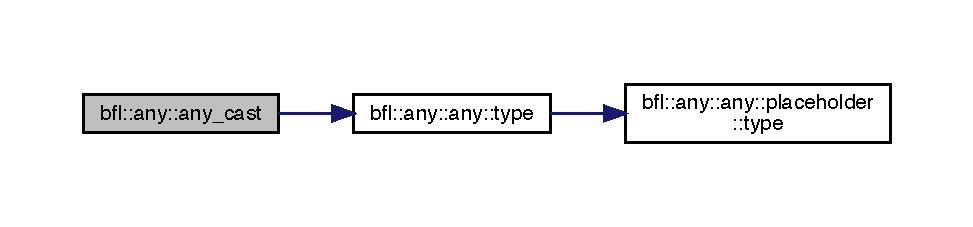
\includegraphics[width=350pt]{namespacebfl_1_1any_a2b5d2dbb287832915598b087083885be_cgraph}
\end{center}
\end{figure}
\mbox{\Hypertarget{namespacebfl_1_1any_aa10ebe32454df7c7769d7391c72f2230}\label{namespacebfl_1_1any_aa10ebe32454df7c7769d7391c72f2230}} 
\index{bfl\+::any@{bfl\+::any}!any\+\_\+cast@{any\+\_\+cast}}
\index{any\+\_\+cast@{any\+\_\+cast}!bfl\+::any@{bfl\+::any}}
\subsubsection{\texorpdfstring{any\+\_\+cast()}{any\_cast()}\hspace{0.1cm}{\footnotesize\ttfamily [4/5]}}
{\footnotesize\ttfamily template$<$typename Value\+Type $>$ \\
Value\+Type bfl\+::any\+::any\+\_\+cast (\begin{DoxyParamCaption}\item[{const \mbox{\hyperlink{classbfl_1_1any_1_1any}{any}} \&}]{operand }\end{DoxyParamCaption})\hspace{0.3cm}{\ttfamily [inline]}}



Performs type-\/safe access to the contained object. 

Throws libanyboost\+::bad\+\_\+any\+\_\+cast if the typeid of the requested Value\+Type does not match that of the contents of operand.


\begin{DoxyParams}{Parameters}
{\em operand} & target any object \\
\hline
\end{DoxyParams}


Definition at line 375 of file any.\+h.



References bfl\+::any\+::any\+::any\+\_\+cast.

\mbox{\Hypertarget{namespacebfl_1_1any_ad3725007dbc3ccb1af3f821dc5a3afd3}\label{namespacebfl_1_1any_ad3725007dbc3ccb1af3f821dc5a3afd3}} 
\index{bfl\+::any@{bfl\+::any}!any\+\_\+cast@{any\+\_\+cast}}
\index{any\+\_\+cast@{any\+\_\+cast}!bfl\+::any@{bfl\+::any}}
\subsubsection{\texorpdfstring{any\+\_\+cast()}{any\_cast()}\hspace{0.1cm}{\footnotesize\ttfamily [5/5]}}
{\footnotesize\ttfamily template$<$typename Value\+Type $>$ \\
Value\+Type bfl\+::any\+::any\+\_\+cast (\begin{DoxyParamCaption}\item[{\mbox{\hyperlink{classbfl_1_1any_1_1any}{any}} \&\&}]{operand }\end{DoxyParamCaption})\hspace{0.3cm}{\ttfamily [inline]}}



Performs type-\/safe access to the contained object. 

Throws libanyboost\+::bad\+\_\+any\+\_\+cast if the typeid of the requested Value\+Type does not match that of the contents of operand.


\begin{DoxyParams}{Parameters}
{\em operand} & target any object \\
\hline
\end{DoxyParams}


Definition at line 391 of file any.\+h.



References bfl\+::any\+::any\+::any\+\_\+cast.

\mbox{\Hypertarget{namespacebfl_1_1any_adb1328ea975e3bf9c0addc1689215bad}\label{namespacebfl_1_1any_adb1328ea975e3bf9c0addc1689215bad}} 
\index{bfl\+::any@{bfl\+::any}!swap@{swap}}
\index{swap@{swap}!bfl\+::any@{bfl\+::any}}
\subsubsection{\texorpdfstring{swap()}{swap()}}
{\footnotesize\ttfamily void bfl\+::any\+::swap (\begin{DoxyParamCaption}\item[{\mbox{\hyperlink{classbfl_1_1any_1_1any}{any}} \&}]{lhs,  }\item[{\mbox{\hyperlink{classbfl_1_1any_1_1any}{any}} \&}]{rhs }\end{DoxyParamCaption})\hspace{0.3cm}{\ttfamily [inline]}, {\ttfamily [noexcept]}}



Overloads the std\+::swap algorithm for std\+::any. 

Swaps the content of two any objects by calling lhs.\+swap(rhs).


\begin{DoxyParams}{Parameters}
{\em lhs} & objects to swap \\
\hline
{\em rhs} & objects to swap \\
\hline
\end{DoxyParams}


Definition at line 287 of file any.\+h.



References bfl\+::any\+::any\+::swap().



Referenced by bfl\+::any\+::any\+::swap().

Here is the call graph for this function\+:
\nopagebreak
\begin{figure}[H]
\begin{center}
\leavevmode
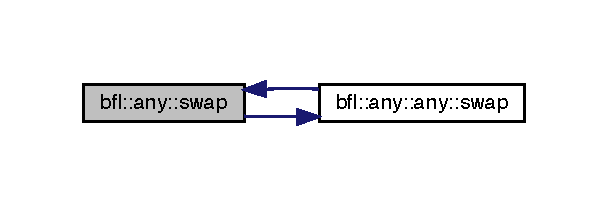
\includegraphics[width=292pt]{namespacebfl_1_1any_adb1328ea975e3bf9c0addc1689215bad_cgraph}
\end{center}
\end{figure}

\hypertarget{namespacebfl_1_1directional__statistics}{}\section{bfl\+:\+:directional\+\_\+statistics Namespace Reference}
\label{namespacebfl_1_1directional__statistics}\index{bfl\+::directional\+\_\+statistics@{bfl\+::directional\+\_\+statistics}}
\subsection*{Functions}
\begin{DoxyCompactItemize}
\item 
Eigen\+::\+Matrix\+Xd \mbox{\hyperlink{namespacebfl_1_1directional__statistics_af9984a4df2b3f6f0bc0c264783181123}{directional\+\_\+add}} (const Eigen\+::\+Ref$<$ const Eigen\+::\+Matrix\+Xd $>$ \&a, const Eigen\+::\+Ref$<$ const Eigen\+::\+Vector\+Xd $>$ \&b)
\item 
Eigen\+::\+Matrix\+Xd \mbox{\hyperlink{namespacebfl_1_1directional__statistics_a18bffca88c7ea5f4ea11d2ad910736fe}{directional\+\_\+sub}} (const Eigen\+::\+Ref$<$ const Eigen\+::\+Matrix\+Xd $>$ \&a, const Eigen\+::\+Ref$<$ const Eigen\+::\+Vector\+Xd $>$ \&b)
\item 
Eigen\+::\+Vector\+Xd \mbox{\hyperlink{namespacebfl_1_1directional__statistics_ad8758aac208bc2baa75aad514a3f53e6}{directional\+\_\+mean}} (const Eigen\+::\+Ref$<$ const Eigen\+::\+Matrix\+Xd $>$ \&a, const Eigen\+::\+Ref$<$ const Eigen\+::\+Vector\+Xd $>$ \&w)
\end{DoxyCompactItemize}


\subsection{Function Documentation}
\mbox{\Hypertarget{namespacebfl_1_1directional__statistics_af9984a4df2b3f6f0bc0c264783181123}\label{namespacebfl_1_1directional__statistics_af9984a4df2b3f6f0bc0c264783181123}} 
\index{bfl\+::directional\+\_\+statistics@{bfl\+::directional\+\_\+statistics}!directional\+\_\+add@{directional\+\_\+add}}
\index{directional\+\_\+add@{directional\+\_\+add}!bfl\+::directional\+\_\+statistics@{bfl\+::directional\+\_\+statistics}}
\subsubsection{\texorpdfstring{directional\+\_\+add()}{directional\_add()}}
{\footnotesize\ttfamily Eigen\+::\+Matrix\+Xd bfl\+::directional\+\_\+statistics\+::directional\+\_\+add (\begin{DoxyParamCaption}\item[{const Eigen\+::\+Ref$<$ const Eigen\+::\+Matrix\+Xd $>$ \&}]{a,  }\item[{const Eigen\+::\+Ref$<$ const Eigen\+::\+Vector\+Xd $>$ \&}]{b }\end{DoxyParamCaption})}



Referenced by bfl\+::sigma\+\_\+point\+::sigma\+\_\+point().

\mbox{\Hypertarget{namespacebfl_1_1directional__statistics_ad8758aac208bc2baa75aad514a3f53e6}\label{namespacebfl_1_1directional__statistics_ad8758aac208bc2baa75aad514a3f53e6}} 
\index{bfl\+::directional\+\_\+statistics@{bfl\+::directional\+\_\+statistics}!directional\+\_\+mean@{directional\+\_\+mean}}
\index{directional\+\_\+mean@{directional\+\_\+mean}!bfl\+::directional\+\_\+statistics@{bfl\+::directional\+\_\+statistics}}
\subsubsection{\texorpdfstring{directional\+\_\+mean()}{directional\_mean()}}
{\footnotesize\ttfamily Eigen\+::\+Vector\+Xd bfl\+::directional\+\_\+statistics\+::directional\+\_\+mean (\begin{DoxyParamCaption}\item[{const Eigen\+::\+Ref$<$ const Eigen\+::\+Matrix\+Xd $>$ \&}]{a,  }\item[{const Eigen\+::\+Ref$<$ const Eigen\+::\+Vector\+Xd $>$ \&}]{w }\end{DoxyParamCaption})}



Referenced by bfl\+::sigma\+\_\+point\+::unscented\+\_\+transform().

\mbox{\Hypertarget{namespacebfl_1_1directional__statistics_a18bffca88c7ea5f4ea11d2ad910736fe}\label{namespacebfl_1_1directional__statistics_a18bffca88c7ea5f4ea11d2ad910736fe}} 
\index{bfl\+::directional\+\_\+statistics@{bfl\+::directional\+\_\+statistics}!directional\+\_\+sub@{directional\+\_\+sub}}
\index{directional\+\_\+sub@{directional\+\_\+sub}!bfl\+::directional\+\_\+statistics@{bfl\+::directional\+\_\+statistics}}
\subsubsection{\texorpdfstring{directional\+\_\+sub()}{directional\_sub()}}
{\footnotesize\ttfamily Eigen\+::\+Matrix\+Xd bfl\+::directional\+\_\+statistics\+::directional\+\_\+sub (\begin{DoxyParamCaption}\item[{const Eigen\+::\+Ref$<$ const Eigen\+::\+Matrix\+Xd $>$ \&}]{a,  }\item[{const Eigen\+::\+Ref$<$ const Eigen\+::\+Vector\+Xd $>$ \&}]{b }\end{DoxyParamCaption})}



Referenced by bfl\+::\+S\+U\+K\+F\+Correction\+::correct\+Step(), and bfl\+::sigma\+\_\+point\+::unscented\+\_\+transform().


\hypertarget{namespacebfl_1_1sigma__point}{}\section{bfl\+:\+:sigma\+\_\+point Namespace Reference}
\label{namespacebfl_1_1sigma__point}\index{bfl\+::sigma\+\_\+point@{bfl\+::sigma\+\_\+point}}
\subsection*{Classes}
\begin{DoxyCompactItemize}
\item 
struct \mbox{\hyperlink{structbfl_1_1sigma__point_1_1UTWeight}{U\+T\+Weight}}
\end{DoxyCompactItemize}
\subsection*{Typedefs}
\begin{DoxyCompactItemize}
\item 
using \mbox{\hyperlink{namespacebfl_1_1sigma__point_aa482c1c98a2280cd8f7635ba81898b4e}{Output\+Size}} = std\+::pair$<$ std\+::size\+\_\+t, std\+::size\+\_\+t $>$
\begin{DoxyCompactList}\small\item\em A Function\+Evaluation return. \end{DoxyCompactList}\item 
using \mbox{\hyperlink{namespacebfl_1_1sigma__point_a6b412638c2556e4c1f84ba10965f785e}{Function\+Evaluation}} = std\+::function$<$ std\+::tuple$<$ bool, \mbox{\hyperlink{namespacebfl_af6b103c6821db1b54452f776fdd9dd02}{bfl\+::\+Data}}, \mbox{\hyperlink{namespacebfl_1_1sigma__point_aa482c1c98a2280cd8f7635ba81898b4e}{Output\+Size}} $>$(const Eigen\+::\+Ref$<$ const Eigen\+::\+Matrix\+Xd $>$ \&)$>$
\end{DoxyCompactItemize}
\subsection*{Functions}
\begin{DoxyCompactItemize}
\item 
void \mbox{\hyperlink{namespacebfl_1_1sigma__point_a2cdca209c158edd6440c2f077b345799}{unscented\+\_\+weights}} (const std\+::size\+\_\+t n, const double alpha, const double beta, const double kappa, Eigen\+::\+Ref$<$ Eigen\+::\+Vector\+Xd $>$ weight\+\_\+mean, Eigen\+::\+Ref$<$ Eigen\+::\+Vector\+Xd $>$ weight\+\_\+covariance, double \&c)
\item 
Eigen\+::\+Matrix\+Xd \mbox{\hyperlink{namespacebfl_1_1sigma__point_ab919aca5fccc30ee2acd5cd966cd9dc9}{sigma\+\_\+point}} (const \mbox{\hyperlink{classbfl_1_1GaussianMixture}{Gaussian\+Mixture}} \&state, const double c)
\item 
std\+::tuple$<$ bool, \mbox{\hyperlink{classbfl_1_1GaussianMixture}{Gaussian\+Mixture}}, Eigen\+::\+Matrix\+Xd $>$ \mbox{\hyperlink{namespacebfl_1_1sigma__point_afe170453152d4f96db4dad71bd9be9a3}{unscented\+\_\+transform}} (const \mbox{\hyperlink{classbfl_1_1GaussianMixture}{Gaussian\+Mixture}} \&input, const \mbox{\hyperlink{structbfl_1_1sigma__point_1_1UTWeight}{U\+T\+Weight}} \&weight, \mbox{\hyperlink{namespacebfl_1_1sigma__point_a6b412638c2556e4c1f84ba10965f785e}{Function\+Evaluation}} function)
\item 
std\+::pair$<$ \mbox{\hyperlink{classbfl_1_1GaussianMixture}{Gaussian\+Mixture}}, Eigen\+::\+Matrix\+Xd $>$ \mbox{\hyperlink{namespacebfl_1_1sigma__point_a49b40777ee901dfbe3752e8f165fb439}{unscented\+\_\+transform}} (const \mbox{\hyperlink{classbfl_1_1GaussianMixture}{Gaussian\+Mixture}} \&state, const \mbox{\hyperlink{structbfl_1_1sigma__point_1_1UTWeight}{U\+T\+Weight}} \&weight, \mbox{\hyperlink{classbfl_1_1StateModel}{State\+Model}} \&state\+\_\+model)
\item 
std\+::pair$<$ \mbox{\hyperlink{classbfl_1_1GaussianMixture}{Gaussian\+Mixture}}, Eigen\+::\+Matrix\+Xd $>$ \mbox{\hyperlink{namespacebfl_1_1sigma__point_a9b4d661460ac0ad28493ae144a6ccee4}{unscented\+\_\+transform}} (const \mbox{\hyperlink{classbfl_1_1GaussianMixture}{Gaussian\+Mixture}} \&state, const \mbox{\hyperlink{structbfl_1_1sigma__point_1_1UTWeight}{U\+T\+Weight}} \&weight, \mbox{\hyperlink{classbfl_1_1StateModel}{State\+Model}} \&state\+\_\+model, \mbox{\hyperlink{classbfl_1_1ExogenousModel}{Exogenous\+Model}} \&exogenous\+\_\+model)
\item 
std\+::pair$<$ \mbox{\hyperlink{classbfl_1_1GaussianMixture}{Gaussian\+Mixture}}, Eigen\+::\+Matrix\+Xd $>$ \mbox{\hyperlink{namespacebfl_1_1sigma__point_ab1a8018531dbd8a28c08dd3418d1976d}{unscented\+\_\+transform}} (const \mbox{\hyperlink{classbfl_1_1GaussianMixture}{Gaussian\+Mixture}} \&state, const \mbox{\hyperlink{structbfl_1_1sigma__point_1_1UTWeight}{U\+T\+Weight}} \&weight, \mbox{\hyperlink{classbfl_1_1AdditiveStateModel}{Additive\+State\+Model}} \&state\+\_\+model)
\item 
std\+::pair$<$ \mbox{\hyperlink{classbfl_1_1GaussianMixture}{Gaussian\+Mixture}}, Eigen\+::\+Matrix\+Xd $>$ \mbox{\hyperlink{namespacebfl_1_1sigma__point_aa14b7405b4800c5382d402b2446f89c6}{unscented\+\_\+transform}} (const \mbox{\hyperlink{classbfl_1_1GaussianMixture}{Gaussian\+Mixture}} \&state, const \mbox{\hyperlink{structbfl_1_1sigma__point_1_1UTWeight}{U\+T\+Weight}} \&weight, \mbox{\hyperlink{classbfl_1_1AdditiveStateModel}{Additive\+State\+Model}} \&state\+\_\+model, \mbox{\hyperlink{classbfl_1_1ExogenousModel}{Exogenous\+Model}} \&exogenous\+\_\+model)
\item 
std\+::pair$<$ \mbox{\hyperlink{classbfl_1_1GaussianMixture}{Gaussian\+Mixture}}, Eigen\+::\+Matrix\+Xd $>$ \mbox{\hyperlink{namespacebfl_1_1sigma__point_ad1df67122c8b838ae669d1f2e0665481}{unscented\+\_\+transform}} (const \mbox{\hyperlink{classbfl_1_1GaussianMixture}{Gaussian\+Mixture}} \&state, const \mbox{\hyperlink{structbfl_1_1sigma__point_1_1UTWeight}{U\+T\+Weight}} \&weight, \mbox{\hyperlink{classbfl_1_1ExogenousModel}{Exogenous\+Model}} \&exogenous\+\_\+model)
\item 
std\+::tuple$<$ bool, \mbox{\hyperlink{classbfl_1_1GaussianMixture}{Gaussian\+Mixture}}, Eigen\+::\+Matrix\+Xd $>$ \mbox{\hyperlink{namespacebfl_1_1sigma__point_a5b51d83e121121ecc6d65e9e5e7d6859}{unscented\+\_\+transform}} (const \mbox{\hyperlink{classbfl_1_1GaussianMixture}{Gaussian\+Mixture}} \&state, const \mbox{\hyperlink{structbfl_1_1sigma__point_1_1UTWeight}{U\+T\+Weight}} \&weight, \mbox{\hyperlink{classbfl_1_1MeasurementModel}{Measurement\+Model}} \&meas\+\_\+model)
\item 
std\+::tuple$<$ bool, \mbox{\hyperlink{classbfl_1_1GaussianMixture}{Gaussian\+Mixture}}, Eigen\+::\+Matrix\+Xd $>$ \mbox{\hyperlink{namespacebfl_1_1sigma__point_a27f6087b127407402338b68bf7853ae6}{unscented\+\_\+transform}} (const \mbox{\hyperlink{classbfl_1_1GaussianMixture}{Gaussian\+Mixture}} \&state, const \mbox{\hyperlink{structbfl_1_1sigma__point_1_1UTWeight}{U\+T\+Weight}} \&weight, \mbox{\hyperlink{classbfl_1_1AdditiveMeasurementModel}{Additive\+Measurement\+Model}} \&meas\+\_\+model)
\end{DoxyCompactItemize}


\subsection{Typedef Documentation}
\mbox{\Hypertarget{namespacebfl_1_1sigma__point_a6b412638c2556e4c1f84ba10965f785e}\label{namespacebfl_1_1sigma__point_a6b412638c2556e4c1f84ba10965f785e}} 
\index{bfl\+::sigma\+\_\+point@{bfl\+::sigma\+\_\+point}!Function\+Evaluation@{Function\+Evaluation}}
\index{Function\+Evaluation@{Function\+Evaluation}!bfl\+::sigma\+\_\+point@{bfl\+::sigma\+\_\+point}}
\subsubsection{\texorpdfstring{Function\+Evaluation}{FunctionEvaluation}}
{\footnotesize\ttfamily using \mbox{\hyperlink{namespacebfl_1_1sigma__point_a6b412638c2556e4c1f84ba10965f785e}{bfl\+::sigma\+\_\+point\+::\+Function\+Evaluation}} = typedef std\+::function$<$std\+::tuple$<$bool, \mbox{\hyperlink{namespacebfl_af6b103c6821db1b54452f776fdd9dd02}{bfl\+::\+Data}}, \mbox{\hyperlink{namespacebfl_1_1sigma__point_aa482c1c98a2280cd8f7635ba81898b4e}{Output\+Size}}$>$(const Eigen\+::\+Ref$<$const Eigen\+::\+Matrix\+Xd$>$\&)$>$}



Definition at line 28 of file sigma\+\_\+point.\+h.

\mbox{\Hypertarget{namespacebfl_1_1sigma__point_aa482c1c98a2280cd8f7635ba81898b4e}\label{namespacebfl_1_1sigma__point_aa482c1c98a2280cd8f7635ba81898b4e}} 
\index{bfl\+::sigma\+\_\+point@{bfl\+::sigma\+\_\+point}!Output\+Size@{Output\+Size}}
\index{Output\+Size@{Output\+Size}!bfl\+::sigma\+\_\+point@{bfl\+::sigma\+\_\+point}}
\subsubsection{\texorpdfstring{Output\+Size}{OutputSize}}
{\footnotesize\ttfamily using \mbox{\hyperlink{namespacebfl_1_1sigma__point_aa482c1c98a2280cd8f7635ba81898b4e}{bfl\+::sigma\+\_\+point\+::\+Output\+Size}} = typedef std\+::pair$<$std\+::size\+\_\+t, std\+::size\+\_\+t$>$}



A Function\+Evaluation return. 


\begin{DoxyItemize}
\item a boolean indicating if the evaluation was successful
\item the output data in the form of \mbox{\hyperlink{namespacebfl_af6b103c6821db1b54452f776fdd9dd02}{bfl\+::\+Data}}
\item the output size as a pair of std\+::size\+\_\+t indicating linear and circular size 
\end{DoxyItemize}

Definition at line 27 of file sigma\+\_\+point.\+h.



\subsection{Function Documentation}
\mbox{\Hypertarget{namespacebfl_1_1sigma__point_ab919aca5fccc30ee2acd5cd966cd9dc9}\label{namespacebfl_1_1sigma__point_ab919aca5fccc30ee2acd5cd966cd9dc9}} 
\index{bfl\+::sigma\+\_\+point@{bfl\+::sigma\+\_\+point}!sigma\+\_\+point@{sigma\+\_\+point}}
\index{sigma\+\_\+point@{sigma\+\_\+point}!bfl\+::sigma\+\_\+point@{bfl\+::sigma\+\_\+point}}
\subsubsection{\texorpdfstring{sigma\+\_\+point()}{sigma\_point()}}
{\footnotesize\ttfamily Matrix\+Xd bfl\+::sigma\+\_\+point\+::sigma\+\_\+point (\begin{DoxyParamCaption}\item[{const \mbox{\hyperlink{classbfl_1_1GaussianMixture}{Gaussian\+Mixture}} \&}]{state,  }\item[{const double}]{c }\end{DoxyParamCaption})}



Definition at line 57 of file sigma\+\_\+point.\+cpp.



References bfl\+::\+Gaussian\+Mixture\+::components, bfl\+::\+Gaussian\+Mixture\+::covariance(), bfl\+::\+Gaussian\+Mixture\+::dim, bfl\+::\+Gaussian\+Mixture\+::dim\+\_\+circular, bfl\+::\+Gaussian\+Mixture\+::dim\+\_\+linear, bfl\+::\+Gaussian\+Mixture\+::dim\+\_\+noise, bfl\+::directional\+\_\+statistics\+::directional\+\_\+add(), and bfl\+::\+Gaussian\+Mixture\+::mean().



Referenced by bfl\+::\+S\+U\+K\+F\+Correction\+::correct\+Step(), and unscented\+\_\+transform().

Here is the call graph for this function\+:
\nopagebreak
\begin{figure}[H]
\begin{center}
\leavevmode
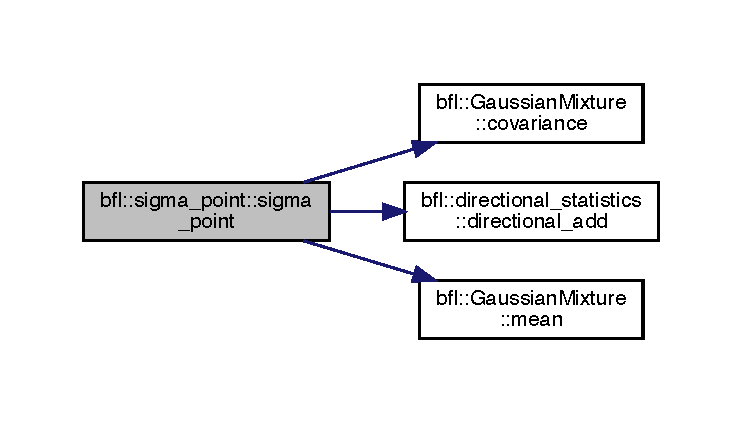
\includegraphics[width=350pt]{namespacebfl_1_1sigma__point_ab919aca5fccc30ee2acd5cd966cd9dc9_cgraph}
\end{center}
\end{figure}
\mbox{\Hypertarget{namespacebfl_1_1sigma__point_afe170453152d4f96db4dad71bd9be9a3}\label{namespacebfl_1_1sigma__point_afe170453152d4f96db4dad71bd9be9a3}} 
\index{bfl\+::sigma\+\_\+point@{bfl\+::sigma\+\_\+point}!unscented\+\_\+transform@{unscented\+\_\+transform}}
\index{unscented\+\_\+transform@{unscented\+\_\+transform}!bfl\+::sigma\+\_\+point@{bfl\+::sigma\+\_\+point}}
\subsubsection{\texorpdfstring{unscented\+\_\+transform()}{unscented\_transform()}\hspace{0.1cm}{\footnotesize\ttfamily [1/8]}}
{\footnotesize\ttfamily std\+::tuple$<$ bool, \mbox{\hyperlink{classbfl_1_1GaussianMixture}{Gaussian\+Mixture}}, Matrix\+Xd $>$ bfl\+::sigma\+\_\+point\+::unscented\+\_\+transform (\begin{DoxyParamCaption}\item[{const \mbox{\hyperlink{classbfl_1_1GaussianMixture}{Gaussian\+Mixture}} \&}]{input,  }\item[{const \mbox{\hyperlink{structbfl_1_1sigma__point_1_1UTWeight}{U\+T\+Weight}} \&}]{weight,  }\item[{\mbox{\hyperlink{namespacebfl_1_1sigma__point_a6b412638c2556e4c1f84ba10965f785e}{Function\+Evaluation}}}]{function }\end{DoxyParamCaption})}



Definition at line 86 of file sigma\+\_\+point.\+cpp.



References bfl\+::any\+::any\+\_\+cast(), bfl\+::sigma\+\_\+point\+::\+U\+T\+Weight\+::c, bfl\+::\+Gaussian\+Mixture\+::components, bfl\+::sigma\+\_\+point\+::\+U\+T\+Weight\+::covariance, bfl\+::\+Gaussian\+Mixture\+::dim, bfl\+::\+Gaussian\+Mixture\+::dim\+\_\+circular, bfl\+::\+Gaussian\+Mixture\+::dim\+\_\+linear, bfl\+::directional\+\_\+statistics\+::directional\+\_\+mean(), bfl\+::directional\+\_\+statistics\+::directional\+\_\+sub(), bfl\+::\+Gaussian\+Mixture\+::mean(), bfl\+::sigma\+\_\+point\+::\+U\+T\+Weight\+::mean, and sigma\+\_\+point().



Referenced by bfl\+::\+U\+K\+F\+Correction\+::correct\+Step(), bfl\+::\+U\+K\+F\+Prediction\+::predict\+Step(), and unscented\+\_\+transform().

Here is the call graph for this function\+:
\nopagebreak
\begin{figure}[H]
\begin{center}
\leavevmode
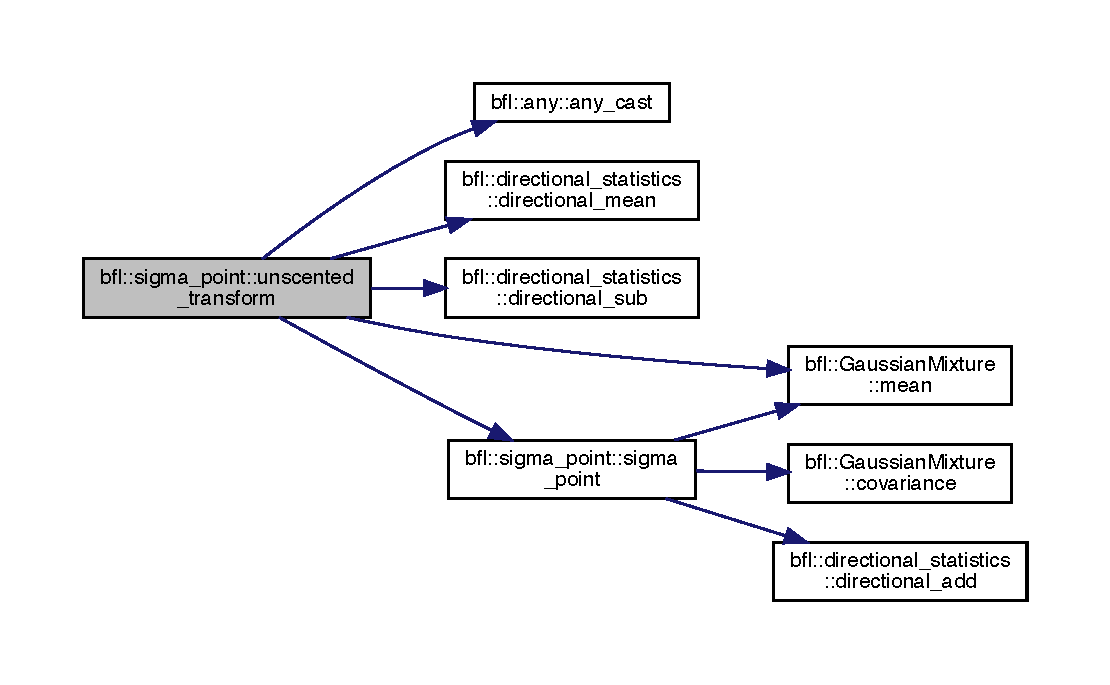
\includegraphics[width=350pt]{namespacebfl_1_1sigma__point_afe170453152d4f96db4dad71bd9be9a3_cgraph}
\end{center}
\end{figure}
\mbox{\Hypertarget{namespacebfl_1_1sigma__point_a49b40777ee901dfbe3752e8f165fb439}\label{namespacebfl_1_1sigma__point_a49b40777ee901dfbe3752e8f165fb439}} 
\index{bfl\+::sigma\+\_\+point@{bfl\+::sigma\+\_\+point}!unscented\+\_\+transform@{unscented\+\_\+transform}}
\index{unscented\+\_\+transform@{unscented\+\_\+transform}!bfl\+::sigma\+\_\+point@{bfl\+::sigma\+\_\+point}}
\subsubsection{\texorpdfstring{unscented\+\_\+transform()}{unscented\_transform()}\hspace{0.1cm}{\footnotesize\ttfamily [2/8]}}
{\footnotesize\ttfamily std\+::pair$<$ \mbox{\hyperlink{classbfl_1_1GaussianMixture}{Gaussian\+Mixture}}, Matrix\+Xd $>$ bfl\+::sigma\+\_\+point\+::unscented\+\_\+transform (\begin{DoxyParamCaption}\item[{const \mbox{\hyperlink{classbfl_1_1GaussianMixture}{Gaussian\+Mixture}} \&}]{state,  }\item[{const \mbox{\hyperlink{structbfl_1_1sigma__point_1_1UTWeight}{U\+T\+Weight}} \&}]{weight,  }\item[{\mbox{\hyperlink{classbfl_1_1StateModel}{State\+Model}} \&}]{state\+\_\+model }\end{DoxyParamCaption})}



Definition at line 143 of file sigma\+\_\+point.\+cpp.



References bfl\+::\+State\+Model\+::get\+Output\+Size(), bfl\+::\+State\+Model\+::motion(), and unscented\+\_\+transform().

Here is the call graph for this function\+:
\nopagebreak
\begin{figure}[H]
\begin{center}
\leavevmode
\includegraphics[width=350pt]{namespacebfl_1_1sigma__point_a49b40777ee901dfbe3752e8f165fb439_cgraph}
\end{center}
\end{figure}
\mbox{\Hypertarget{namespacebfl_1_1sigma__point_a9b4d661460ac0ad28493ae144a6ccee4}\label{namespacebfl_1_1sigma__point_a9b4d661460ac0ad28493ae144a6ccee4}} 
\index{bfl\+::sigma\+\_\+point@{bfl\+::sigma\+\_\+point}!unscented\+\_\+transform@{unscented\+\_\+transform}}
\index{unscented\+\_\+transform@{unscented\+\_\+transform}!bfl\+::sigma\+\_\+point@{bfl\+::sigma\+\_\+point}}
\subsubsection{\texorpdfstring{unscented\+\_\+transform()}{unscented\_transform()}\hspace{0.1cm}{\footnotesize\ttfamily [3/8]}}
{\footnotesize\ttfamily std\+::pair$<$ \mbox{\hyperlink{classbfl_1_1GaussianMixture}{Gaussian\+Mixture}}, Matrix\+Xd $>$ bfl\+::sigma\+\_\+point\+::unscented\+\_\+transform (\begin{DoxyParamCaption}\item[{const \mbox{\hyperlink{classbfl_1_1GaussianMixture}{Gaussian\+Mixture}} \&}]{state,  }\item[{const \mbox{\hyperlink{structbfl_1_1sigma__point_1_1UTWeight}{U\+T\+Weight}} \&}]{weight,  }\item[{\mbox{\hyperlink{classbfl_1_1StateModel}{State\+Model}} \&}]{state\+\_\+model,  }\item[{\mbox{\hyperlink{classbfl_1_1ExogenousModel}{Exogenous\+Model}} \&}]{exogenous\+\_\+model }\end{DoxyParamCaption})}



Definition at line 166 of file sigma\+\_\+point.\+cpp.



References bfl\+::\+State\+Model\+::get\+Output\+Size(), bfl\+::\+State\+Model\+::motion(), bfl\+::\+Exogenous\+Model\+::propagate(), and unscented\+\_\+transform().

Here is the call graph for this function\+:
\nopagebreak
\begin{figure}[H]
\begin{center}
\leavevmode
\includegraphics[width=350pt]{namespacebfl_1_1sigma__point_a9b4d661460ac0ad28493ae144a6ccee4_cgraph}
\end{center}
\end{figure}
\mbox{\Hypertarget{namespacebfl_1_1sigma__point_ab1a8018531dbd8a28c08dd3418d1976d}\label{namespacebfl_1_1sigma__point_ab1a8018531dbd8a28c08dd3418d1976d}} 
\index{bfl\+::sigma\+\_\+point@{bfl\+::sigma\+\_\+point}!unscented\+\_\+transform@{unscented\+\_\+transform}}
\index{unscented\+\_\+transform@{unscented\+\_\+transform}!bfl\+::sigma\+\_\+point@{bfl\+::sigma\+\_\+point}}
\subsubsection{\texorpdfstring{unscented\+\_\+transform()}{unscented\_transform()}\hspace{0.1cm}{\footnotesize\ttfamily [4/8]}}
{\footnotesize\ttfamily std\+::pair$<$ \mbox{\hyperlink{classbfl_1_1GaussianMixture}{Gaussian\+Mixture}}, Matrix\+Xd $>$ bfl\+::sigma\+\_\+point\+::unscented\+\_\+transform (\begin{DoxyParamCaption}\item[{const \mbox{\hyperlink{classbfl_1_1GaussianMixture}{Gaussian\+Mixture}} \&}]{state,  }\item[{const \mbox{\hyperlink{structbfl_1_1sigma__point_1_1UTWeight}{U\+T\+Weight}} \&}]{weight,  }\item[{\mbox{\hyperlink{classbfl_1_1AdditiveStateModel}{Additive\+State\+Model}} \&}]{state\+\_\+model }\end{DoxyParamCaption})}



Definition at line 194 of file sigma\+\_\+point.\+cpp.



References bfl\+::\+Gaussian\+Mixture\+::components, bfl\+::\+Gaussian\+Mixture\+::covariance(), bfl\+::\+State\+Model\+::get\+Noise\+Covariance\+Matrix(), bfl\+::\+State\+Model\+::get\+Output\+Size(), bfl\+::\+State\+Model\+::propagate(), and unscented\+\_\+transform().

Here is the call graph for this function\+:
\nopagebreak
\begin{figure}[H]
\begin{center}
\leavevmode
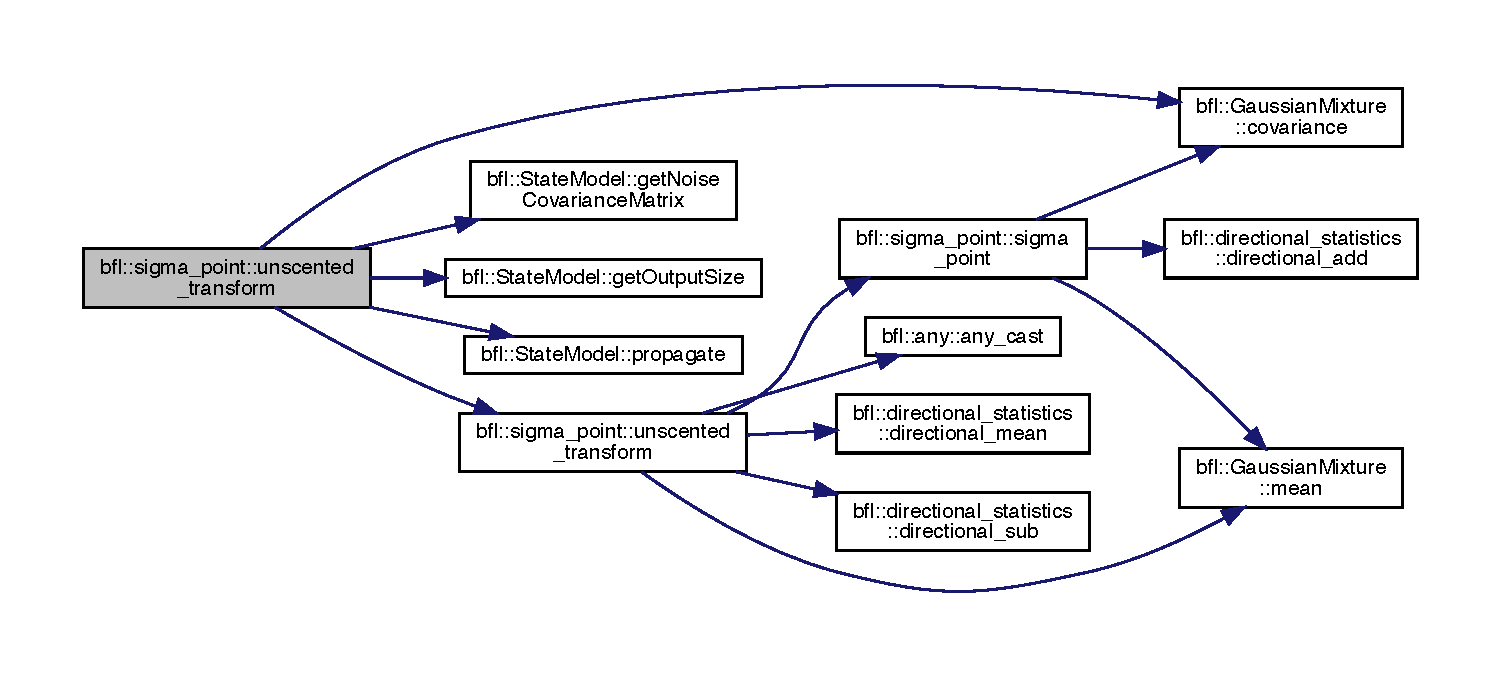
\includegraphics[width=350pt]{namespacebfl_1_1sigma__point_ab1a8018531dbd8a28c08dd3418d1976d_cgraph}
\end{center}
\end{figure}
\mbox{\Hypertarget{namespacebfl_1_1sigma__point_aa14b7405b4800c5382d402b2446f89c6}\label{namespacebfl_1_1sigma__point_aa14b7405b4800c5382d402b2446f89c6}} 
\index{bfl\+::sigma\+\_\+point@{bfl\+::sigma\+\_\+point}!unscented\+\_\+transform@{unscented\+\_\+transform}}
\index{unscented\+\_\+transform@{unscented\+\_\+transform}!bfl\+::sigma\+\_\+point@{bfl\+::sigma\+\_\+point}}
\subsubsection{\texorpdfstring{unscented\+\_\+transform()}{unscented\_transform()}\hspace{0.1cm}{\footnotesize\ttfamily [5/8]}}
{\footnotesize\ttfamily std\+::pair$<$ \mbox{\hyperlink{classbfl_1_1GaussianMixture}{Gaussian\+Mixture}}, Matrix\+Xd $>$ bfl\+::sigma\+\_\+point\+::unscented\+\_\+transform (\begin{DoxyParamCaption}\item[{const \mbox{\hyperlink{classbfl_1_1GaussianMixture}{Gaussian\+Mixture}} \&}]{state,  }\item[{const \mbox{\hyperlink{structbfl_1_1sigma__point_1_1UTWeight}{U\+T\+Weight}} \&}]{weight,  }\item[{\mbox{\hyperlink{classbfl_1_1AdditiveStateModel}{Additive\+State\+Model}} \&}]{state\+\_\+model,  }\item[{\mbox{\hyperlink{classbfl_1_1ExogenousModel}{Exogenous\+Model}} \&}]{exogenous\+\_\+model }\end{DoxyParamCaption})}



Definition at line 223 of file sigma\+\_\+point.\+cpp.



References bfl\+::\+Gaussian\+Mixture\+::components, bfl\+::\+Gaussian\+Mixture\+::covariance(), bfl\+::\+State\+Model\+::get\+Noise\+Covariance\+Matrix(), bfl\+::\+State\+Model\+::get\+Output\+Size(), bfl\+::\+Exogenous\+Model\+::propagate(), bfl\+::\+State\+Model\+::propagate(), and unscented\+\_\+transform().

Here is the call graph for this function\+:
\nopagebreak
\begin{figure}[H]
\begin{center}
\leavevmode
\includegraphics[width=350pt]{namespacebfl_1_1sigma__point_aa14b7405b4800c5382d402b2446f89c6_cgraph}
\end{center}
\end{figure}
\mbox{\Hypertarget{namespacebfl_1_1sigma__point_ad1df67122c8b838ae669d1f2e0665481}\label{namespacebfl_1_1sigma__point_ad1df67122c8b838ae669d1f2e0665481}} 
\index{bfl\+::sigma\+\_\+point@{bfl\+::sigma\+\_\+point}!unscented\+\_\+transform@{unscented\+\_\+transform}}
\index{unscented\+\_\+transform@{unscented\+\_\+transform}!bfl\+::sigma\+\_\+point@{bfl\+::sigma\+\_\+point}}
\subsubsection{\texorpdfstring{unscented\+\_\+transform()}{unscented\_transform()}\hspace{0.1cm}{\footnotesize\ttfamily [6/8]}}
{\footnotesize\ttfamily std\+::pair$<$ \mbox{\hyperlink{classbfl_1_1GaussianMixture}{Gaussian\+Mixture}}, Matrix\+Xd $>$ bfl\+::sigma\+\_\+point\+::unscented\+\_\+transform (\begin{DoxyParamCaption}\item[{const \mbox{\hyperlink{classbfl_1_1GaussianMixture}{Gaussian\+Mixture}} \&}]{state,  }\item[{const \mbox{\hyperlink{structbfl_1_1sigma__point_1_1UTWeight}{U\+T\+Weight}} \&}]{weight,  }\item[{\mbox{\hyperlink{classbfl_1_1ExogenousModel}{Exogenous\+Model}} \&}]{exogenous\+\_\+model }\end{DoxyParamCaption})}



Definition at line 258 of file sigma\+\_\+point.\+cpp.



References bfl\+::\+Exogenous\+Model\+::get\+Output\+Size(), bfl\+::\+Exogenous\+Model\+::propagate(), and unscented\+\_\+transform().

Here is the call graph for this function\+:
\nopagebreak
\begin{figure}[H]
\begin{center}
\leavevmode
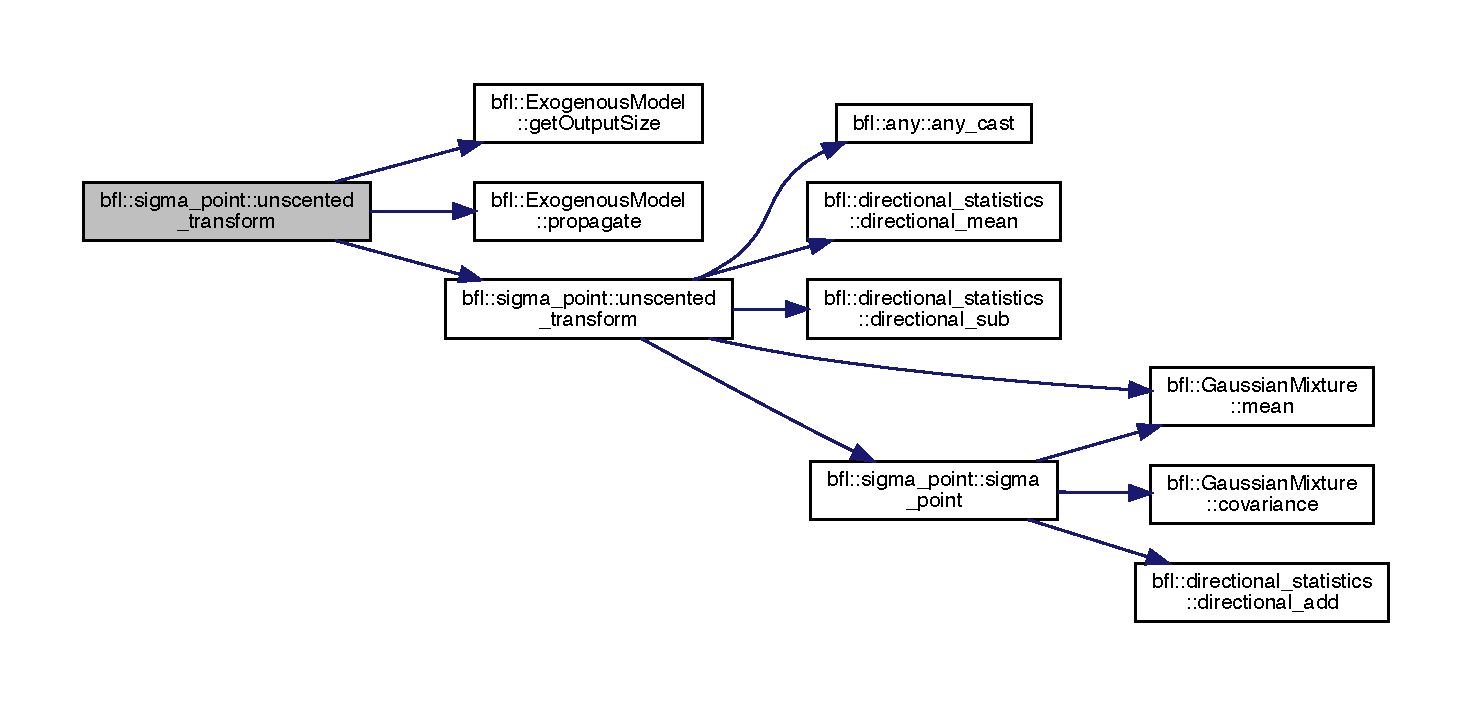
\includegraphics[width=350pt]{namespacebfl_1_1sigma__point_ad1df67122c8b838ae669d1f2e0665481_cgraph}
\end{center}
\end{figure}
\mbox{\Hypertarget{namespacebfl_1_1sigma__point_a5b51d83e121121ecc6d65e9e5e7d6859}\label{namespacebfl_1_1sigma__point_a5b51d83e121121ecc6d65e9e5e7d6859}} 
\index{bfl\+::sigma\+\_\+point@{bfl\+::sigma\+\_\+point}!unscented\+\_\+transform@{unscented\+\_\+transform}}
\index{unscented\+\_\+transform@{unscented\+\_\+transform}!bfl\+::sigma\+\_\+point@{bfl\+::sigma\+\_\+point}}
\subsubsection{\texorpdfstring{unscented\+\_\+transform()}{unscented\_transform()}\hspace{0.1cm}{\footnotesize\ttfamily [7/8]}}
{\footnotesize\ttfamily std\+::tuple$<$ bool, \mbox{\hyperlink{classbfl_1_1GaussianMixture}{Gaussian\+Mixture}}, Matrix\+Xd $>$ bfl\+::sigma\+\_\+point\+::unscented\+\_\+transform (\begin{DoxyParamCaption}\item[{const \mbox{\hyperlink{classbfl_1_1GaussianMixture}{Gaussian\+Mixture}} \&}]{state,  }\item[{const \mbox{\hyperlink{structbfl_1_1sigma__point_1_1UTWeight}{U\+T\+Weight}} \&}]{weight,  }\item[{\mbox{\hyperlink{classbfl_1_1MeasurementModel}{Measurement\+Model}} \&}]{meas\+\_\+model }\end{DoxyParamCaption})}



Definition at line 283 of file sigma\+\_\+point.\+cpp.



References bfl\+::\+Measurement\+Model\+::get\+Output\+Size(), bfl\+::\+Measurement\+Model\+::predicted\+Measure(), and unscented\+\_\+transform().

Here is the call graph for this function\+:
\nopagebreak
\begin{figure}[H]
\begin{center}
\leavevmode
\includegraphics[width=350pt]{namespacebfl_1_1sigma__point_a5b51d83e121121ecc6d65e9e5e7d6859_cgraph}
\end{center}
\end{figure}
\mbox{\Hypertarget{namespacebfl_1_1sigma__point_a27f6087b127407402338b68bf7853ae6}\label{namespacebfl_1_1sigma__point_a27f6087b127407402338b68bf7853ae6}} 
\index{bfl\+::sigma\+\_\+point@{bfl\+::sigma\+\_\+point}!unscented\+\_\+transform@{unscented\+\_\+transform}}
\index{unscented\+\_\+transform@{unscented\+\_\+transform}!bfl\+::sigma\+\_\+point@{bfl\+::sigma\+\_\+point}}
\subsubsection{\texorpdfstring{unscented\+\_\+transform()}{unscented\_transform()}\hspace{0.1cm}{\footnotesize\ttfamily [8/8]}}
{\footnotesize\ttfamily std\+::tuple$<$ bool, \mbox{\hyperlink{classbfl_1_1GaussianMixture}{Gaussian\+Mixture}}, Matrix\+Xd $>$ bfl\+::sigma\+\_\+point\+::unscented\+\_\+transform (\begin{DoxyParamCaption}\item[{const \mbox{\hyperlink{classbfl_1_1GaussianMixture}{Gaussian\+Mixture}} \&}]{state,  }\item[{const \mbox{\hyperlink{structbfl_1_1sigma__point_1_1UTWeight}{U\+T\+Weight}} \&}]{weight,  }\item[{\mbox{\hyperlink{classbfl_1_1AdditiveMeasurementModel}{Additive\+Measurement\+Model}} \&}]{meas\+\_\+model }\end{DoxyParamCaption})}



Definition at line 309 of file sigma\+\_\+point.\+cpp.



References bfl\+::\+Gaussian\+Mixture\+::components, bfl\+::\+Gaussian\+Mixture\+::covariance(), bfl\+::\+Measurement\+Model\+::get\+Noise\+Covariance\+Matrix(), bfl\+::\+Measurement\+Model\+::get\+Output\+Size(), bfl\+::\+Measurement\+Model\+::predicted\+Measure(), and unscented\+\_\+transform().

Here is the call graph for this function\+:
\nopagebreak
\begin{figure}[H]
\begin{center}
\leavevmode
\includegraphics[width=350pt]{namespacebfl_1_1sigma__point_a27f6087b127407402338b68bf7853ae6_cgraph}
\end{center}
\end{figure}
\mbox{\Hypertarget{namespacebfl_1_1sigma__point_a2cdca209c158edd6440c2f077b345799}\label{namespacebfl_1_1sigma__point_a2cdca209c158edd6440c2f077b345799}} 
\index{bfl\+::sigma\+\_\+point@{bfl\+::sigma\+\_\+point}!unscented\+\_\+weights@{unscented\+\_\+weights}}
\index{unscented\+\_\+weights@{unscented\+\_\+weights}!bfl\+::sigma\+\_\+point@{bfl\+::sigma\+\_\+point}}
\subsubsection{\texorpdfstring{unscented\+\_\+weights()}{unscented\_weights()}}
{\footnotesize\ttfamily void bfl\+::sigma\+\_\+point\+::unscented\+\_\+weights (\begin{DoxyParamCaption}\item[{const std\+::size\+\_\+t}]{n,  }\item[{const double}]{alpha,  }\item[{const double}]{beta,  }\item[{const double}]{kappa,  }\item[{Eigen\+::\+Ref$<$ Eigen\+::\+Vector\+Xd $>$}]{weight\+\_\+mean,  }\item[{Eigen\+::\+Ref$<$ Eigen\+::\+Vector\+Xd $>$}]{weight\+\_\+covariance,  }\item[{double \&}]{c }\end{DoxyParamCaption})}



Referenced by bfl\+::sigma\+\_\+point\+::\+U\+T\+Weight\+::\+U\+T\+Weight().


\hypertarget{namespacebfl_1_1utils}{}\section{bfl\+:\+:utils Namespace Reference}
\label{namespacebfl_1_1utils}\index{bfl\+::utils@{bfl\+::utils}}
\subsection*{Functions}
\begin{DoxyCompactItemize}
\item 
{\footnotesize template$<$typename T , typename ... Args$>$ }\\std\+::unique\+\_\+ptr$<$ T $>$ \mbox{\hyperlink{namespacebfl_1_1utils_ad9e9288a23debabef8314ac0d1006e66}{make\+\_\+unique}} (Args \&\&...args)
\begin{DoxyCompactList}\small\item\em Constructs an object of type T and wraps it in a std\+::unique\+\_\+ptr. \end{DoxyCompactList}\item 
double \mbox{\hyperlink{namespacebfl_1_1utils_a137b996032449ce79a5638cbcbb73966}{log\+\_\+sum\+\_\+exp}} (const Eigen\+::\+Ref$<$ const Eigen\+::\+Vector\+Xd $>$ \&arguments)
\begin{DoxyCompactList}\small\item\em Return the logarithm of the sum of exponentials. \end{DoxyCompactList}\end{DoxyCompactItemize}


\subsection{Function Documentation}
\mbox{\Hypertarget{namespacebfl_1_1utils_a137b996032449ce79a5638cbcbb73966}\label{namespacebfl_1_1utils_a137b996032449ce79a5638cbcbb73966}} 
\index{bfl\+::utils@{bfl\+::utils}!log\+\_\+sum\+\_\+exp@{log\+\_\+sum\+\_\+exp}}
\index{log\+\_\+sum\+\_\+exp@{log\+\_\+sum\+\_\+exp}!bfl\+::utils@{bfl\+::utils}}
\subsubsection{\texorpdfstring{log\+\_\+sum\+\_\+exp()}{log\_sum\_exp()}}
{\footnotesize\ttfamily double bfl\+::utils\+::log\+\_\+sum\+\_\+exp (\begin{DoxyParamCaption}\item[{const Eigen\+::\+Ref$<$ const Eigen\+::\+Vector\+Xd $>$ \&}]{arguments }\end{DoxyParamCaption})}



Return the logarithm of the sum of exponentials. 



Referenced by bfl\+::\+S\+I\+S\+::filtering\+Step(), and bfl\+::\+Resampling\+With\+Prior\+::resample().

\mbox{\Hypertarget{namespacebfl_1_1utils_ad9e9288a23debabef8314ac0d1006e66}\label{namespacebfl_1_1utils_ad9e9288a23debabef8314ac0d1006e66}} 
\index{bfl\+::utils@{bfl\+::utils}!make\+\_\+unique@{make\+\_\+unique}}
\index{make\+\_\+unique@{make\+\_\+unique}!bfl\+::utils@{bfl\+::utils}}
\subsubsection{\texorpdfstring{make\+\_\+unique()}{make\_unique()}}
{\footnotesize\ttfamily template$<$typename T , typename ... Args$>$ \\
std\+::unique\+\_\+ptr$<$T$>$ bfl\+::utils\+::make\+\_\+unique (\begin{DoxyParamCaption}\item[{Args \&\&...}]{args }\end{DoxyParamCaption})}



Constructs an object of type T and wraps it in a std\+::unique\+\_\+ptr. 

Constructs a non-\/array type T. The arguments args are passed to the constructor of T. This overload only participates in overload resolution if T is not an array type. The function is equivalent to\+: unique\+\_\+ptr$<$\+T$>$(new T(std\+::forward$<$\+Args$>$(args)...))

\begin{DoxyNote}{Note}
Unlike std\+::make\+\_\+shared (which has std\+::allocate\+\_\+shared), std\+::make\+\_\+unique does not have an allocator-\/aware counterpart. A hypothetical allocate\+\_\+unique would be required to invent the deleter type D for the unique\+\_\+ptr$<$\+T,\+D$>$ it returns which would contain an allocator object and invoke both destroy and deallocate in its operator().
\end{DoxyNote}

\begin{DoxyParams}{Parameters}
{\em args} & list of arguments with which an instance of T will be constructed.\\
\hline
\end{DoxyParams}
May throw std\+::bad\+\_\+alloc or any exception thrown by the constructor of T. If an exception is thrown, this function has no effect.

\begin{DoxyReturn}{Returns}
std\+::unique\+\_\+ptr of an instance of type T. 
\end{DoxyReturn}


Definition at line 46 of file utils.\+h.


\chapter{Class Documentation}
\hypertarget{classbfl_1_1AdditiveMeasurementModel}{}\section{bfl\+:\+:Additive\+Measurement\+Model Class Reference}
\label{classbfl_1_1AdditiveMeasurementModel}\index{bfl\+::\+Additive\+Measurement\+Model@{bfl\+::\+Additive\+Measurement\+Model}}


{\ttfamily \#include $<$Additive\+Measurement\+Model.\+h$>$}



Inheritance diagram for bfl\+:\+:Additive\+Measurement\+Model\+:
\nopagebreak
\begin{figure}[H]
\begin{center}
\leavevmode
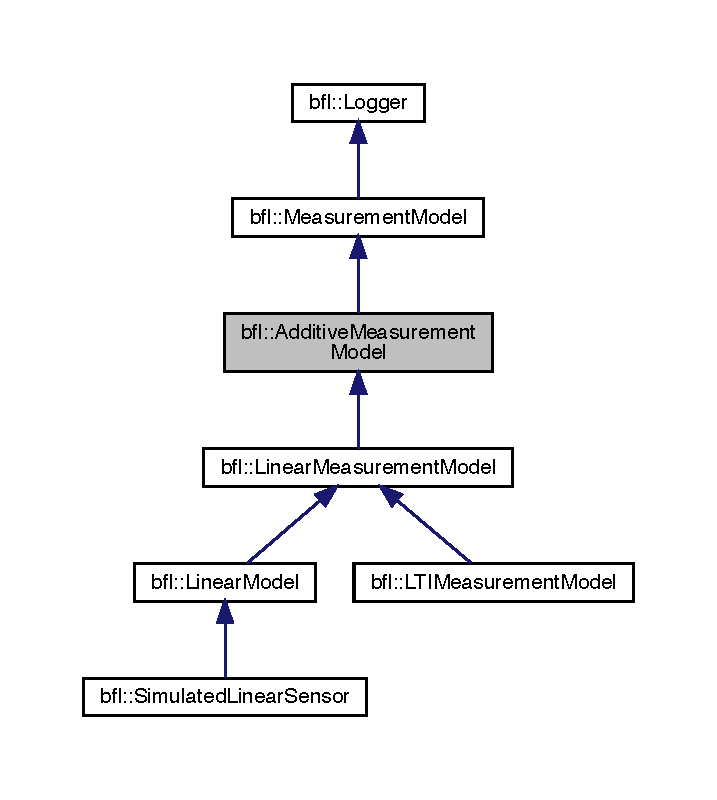
\includegraphics[width=344pt]{classbfl_1_1AdditiveMeasurementModel__inherit__graph}
\end{center}
\end{figure}
\subsection*{Public Member Functions}
\begin{DoxyCompactItemize}
\item 
virtual \mbox{\hyperlink{classbfl_1_1AdditiveMeasurementModel_abe43cf581cf83131a74557cd265ea200}{$\sim$\+Additive\+Measurement\+Model}} () noexcept
\item 
virtual std\+::pair$<$ bool, \mbox{\hyperlink{namespacebfl_af6b103c6821db1b54452f776fdd9dd02}{bfl\+::\+Data}} $>$ \mbox{\hyperlink{classbfl_1_1MeasurementModel_ad372b720cef4e6bc0ac2489f4098bfc9}{measure}} () const =0
\item 
virtual std\+::pair$<$ bool, \mbox{\hyperlink{namespacebfl_af6b103c6821db1b54452f776fdd9dd02}{bfl\+::\+Data}} $>$ \mbox{\hyperlink{classbfl_1_1MeasurementModel_a8fc8798aa2db48f428d4ce59b33b5307}{predicted\+Measure}} (const Eigen\+::\+Ref$<$ const Eigen\+::\+Matrix\+Xd $>$ \&cur\+\_\+states) const =0
\item 
virtual std\+::pair$<$ bool, \mbox{\hyperlink{namespacebfl_af6b103c6821db1b54452f776fdd9dd02}{bfl\+::\+Data}} $>$ \mbox{\hyperlink{classbfl_1_1MeasurementModel_aa06e0643805551a981bcc013ad44c829}{innovation}} (const \mbox{\hyperlink{namespacebfl_af6b103c6821db1b54452f776fdd9dd02}{bfl\+::\+Data}} \&predicted\+\_\+measurements, const \mbox{\hyperlink{namespacebfl_af6b103c6821db1b54452f776fdd9dd02}{bfl\+::\+Data}} \&measurements) const =0
\item 
virtual std\+::pair$<$ bool, Eigen\+::\+Matrix\+Xd $>$ \mbox{\hyperlink{classbfl_1_1MeasurementModel_af25f42076b69e0c6cab47d36d796536f}{get\+Noise\+Covariance\+Matrix}} () const
\item 
virtual bool \mbox{\hyperlink{classbfl_1_1MeasurementModel_af97e18b52d1a3f365dd5982b8cc4aff7}{set\+Property}} (const std\+::string \&property)
\item 
virtual bool \mbox{\hyperlink{classbfl_1_1MeasurementModel_a67ef096c5b3682252582aec75498089d}{freeze\+Measurements}} ()=0
\item 
virtual std\+::pair$<$ std\+::size\+\_\+t, std\+::size\+\_\+t $>$ \mbox{\hyperlink{classbfl_1_1MeasurementModel_a6cca2022b576c9dbb61e73b83a10c6ee}{get\+Output\+Size}} () const =0
\item 
bool \mbox{\hyperlink{classbfl_1_1Logger_ae94b97b6e8d7902e8ce048384813122e}{enable\+\_\+log}} (const std\+::string \&prefix\+\_\+path, const std\+::string \&prefix\+\_\+name)
\item 
bool \mbox{\hyperlink{classbfl_1_1Logger_a440467a28ccc46490d767fe0ef6f556a}{disable\+\_\+log}} ()
\item 
std\+::string \mbox{\hyperlink{classbfl_1_1Logger_a56cf1a4e712bf23d9978420a8a59a62b}{get\+\_\+prefix\+\_\+path}} () const
\item 
std\+::string \mbox{\hyperlink{classbfl_1_1Logger_a913a795b7bfbf378815eeb342d68a7c0}{get\+\_\+prefix\+\_\+name}} () const
\item 
{\footnotesize template$<$typename Datum\+Type $>$ }\\void \mbox{\hyperlink{classbfl_1_1Logger_a1033ff31398484f2132f84fd140da9e3}{logger}} (Datum\+Type datum)
\item 
{\footnotesize template$<$typename... Data\+Type$>$ }\\void \mbox{\hyperlink{classbfl_1_1Logger_aca2086c9256e5c404872b91f7f25b97d}{logger}} (Data\+Type... data)
\item 
{\footnotesize template$<$typename Datum\+Type $>$ }\\void \mbox{\hyperlink{classbfl_1_1Logger_a50b1c109730fa98f66e66f420f0158fe}{logger}} (Datum\+Type datum) const
\item 
{\footnotesize template$<$typename... Data\+Type$>$ }\\void \mbox{\hyperlink{classbfl_1_1Logger_a0f0cf7ce956546d94dfb1feb7cebf171}{logger}} (Data\+Type... data) const
\end{DoxyCompactItemize}
\subsection*{Protected Member Functions}
\begin{DoxyCompactItemize}
\item 
virtual std\+::vector$<$ std\+::string $>$ \mbox{\hyperlink{classbfl_1_1Logger_a328ceaa8e70e6918f11142b12b8be217}{log\+\_\+filenames}} (const std\+::string \&prefix\+\_\+path, const std\+::string \&prefix\+\_\+name)
\item 
virtual void \mbox{\hyperlink{classbfl_1_1Logger_ad44f46593cb8c4c87c1178eb326e2f64}{log}} ()
\end{DoxyCompactItemize}


\subsection{Detailed Description}


Definition at line 11 of file Additive\+Measurement\+Model.\+h.



\subsection{Constructor \& Destructor Documentation}
\mbox{\Hypertarget{classbfl_1_1AdditiveMeasurementModel_abe43cf581cf83131a74557cd265ea200}\label{classbfl_1_1AdditiveMeasurementModel_abe43cf581cf83131a74557cd265ea200}} 
\index{bfl\+::\+Additive\+Measurement\+Model@{bfl\+::\+Additive\+Measurement\+Model}!````~Additive\+Measurement\+Model@{$\sim$\+Additive\+Measurement\+Model}}
\index{````~Additive\+Measurement\+Model@{$\sim$\+Additive\+Measurement\+Model}!bfl\+::\+Additive\+Measurement\+Model@{bfl\+::\+Additive\+Measurement\+Model}}
\subsubsection{\texorpdfstring{$\sim$\+Additive\+Measurement\+Model()}{~AdditiveMeasurementModel()}}
{\footnotesize\ttfamily Additive\+Measurement\+Model\+::$\sim$\+Additive\+Measurement\+Model (\begin{DoxyParamCaption}{ }\end{DoxyParamCaption})\hspace{0.3cm}{\ttfamily [virtual]}, {\ttfamily [noexcept]}}



Definition at line 5 of file Additive\+Measurement\+Model.\+cpp.



\subsection{Member Function Documentation}
\mbox{\Hypertarget{classbfl_1_1Logger_a440467a28ccc46490d767fe0ef6f556a}\label{classbfl_1_1Logger_a440467a28ccc46490d767fe0ef6f556a}} 
\index{bfl\+::\+Additive\+Measurement\+Model@{bfl\+::\+Additive\+Measurement\+Model}!disable\+\_\+log@{disable\+\_\+log}}
\index{disable\+\_\+log@{disable\+\_\+log}!bfl\+::\+Additive\+Measurement\+Model@{bfl\+::\+Additive\+Measurement\+Model}}
\subsubsection{\texorpdfstring{disable\+\_\+log()}{disable\_log()}}
{\footnotesize\ttfamily bool Logger\+::disable\+\_\+log (\begin{DoxyParamCaption}{ }\end{DoxyParamCaption})\hspace{0.3cm}{\ttfamily [inherited]}}



Definition at line 58 of file Logger.\+cpp.



References bfl\+::\+Logger\+::file\+\_\+names\+\_\+, bfl\+::\+Logger\+::log\+\_\+enabled\+\_\+, and bfl\+::\+Logger\+::log\+\_\+files\+\_\+.



Referenced by bfl\+::\+Logger\+::$\sim$\+Logger().

\mbox{\Hypertarget{classbfl_1_1Logger_ae94b97b6e8d7902e8ce048384813122e}\label{classbfl_1_1Logger_ae94b97b6e8d7902e8ce048384813122e}} 
\index{bfl\+::\+Additive\+Measurement\+Model@{bfl\+::\+Additive\+Measurement\+Model}!enable\+\_\+log@{enable\+\_\+log}}
\index{enable\+\_\+log@{enable\+\_\+log}!bfl\+::\+Additive\+Measurement\+Model@{bfl\+::\+Additive\+Measurement\+Model}}
\subsubsection{\texorpdfstring{enable\+\_\+log()}{enable\_log()}}
{\footnotesize\ttfamily bool Logger\+::enable\+\_\+log (\begin{DoxyParamCaption}\item[{const std\+::string \&}]{prefix\+\_\+path,  }\item[{const std\+::string \&}]{prefix\+\_\+name }\end{DoxyParamCaption})\hspace{0.3cm}{\ttfamily [inherited]}}



Definition at line 15 of file Logger.\+cpp.



References bfl\+::\+Logger\+::file\+\_\+names\+\_\+, bfl\+::\+Logger\+::log\+\_\+enabled\+\_\+, bfl\+::\+Logger\+::log\+\_\+filenames(), and bfl\+::\+Logger\+::log\+\_\+files\+\_\+.

Here is the call graph for this function\+:
\nopagebreak
\begin{figure}[H]
\begin{center}
\leavevmode
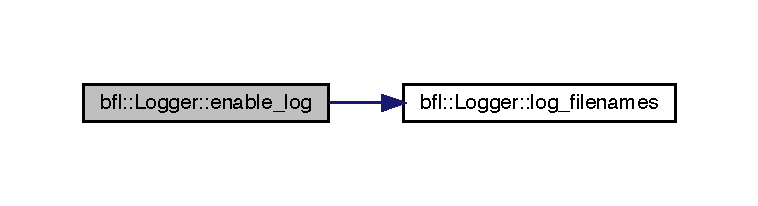
\includegraphics[width=350pt]{classbfl_1_1Logger_ae94b97b6e8d7902e8ce048384813122e_cgraph}
\end{center}
\end{figure}
\mbox{\Hypertarget{classbfl_1_1MeasurementModel_a67ef096c5b3682252582aec75498089d}\label{classbfl_1_1MeasurementModel_a67ef096c5b3682252582aec75498089d}} 
\index{bfl\+::\+Additive\+Measurement\+Model@{bfl\+::\+Additive\+Measurement\+Model}!freeze\+Measurements@{freeze\+Measurements}}
\index{freeze\+Measurements@{freeze\+Measurements}!bfl\+::\+Additive\+Measurement\+Model@{bfl\+::\+Additive\+Measurement\+Model}}
\subsubsection{\texorpdfstring{freeze\+Measurements()}{freezeMeasurements()}}
{\footnotesize\ttfamily virtual bool bfl\+::\+Measurement\+Model\+::freeze\+Measurements (\begin{DoxyParamCaption}{ }\end{DoxyParamCaption})\hspace{0.3cm}{\ttfamily [pure virtual]}, {\ttfamily [inherited]}}



Implemented in \mbox{\hyperlink{classbfl_1_1MeasurementModelDecorator_a17d5fb12bfa048ca56160f745f112e32}{bfl\+::\+Measurement\+Model\+Decorator}}, and \mbox{\hyperlink{classbfl_1_1SimulatedLinearSensor_a683f147d792a79c5ad4c6746210dfdee}{bfl\+::\+Simulated\+Linear\+Sensor}}.

\mbox{\Hypertarget{classbfl_1_1Logger_a913a795b7bfbf378815eeb342d68a7c0}\label{classbfl_1_1Logger_a913a795b7bfbf378815eeb342d68a7c0}} 
\index{bfl\+::\+Additive\+Measurement\+Model@{bfl\+::\+Additive\+Measurement\+Model}!get\+\_\+prefix\+\_\+name@{get\+\_\+prefix\+\_\+name}}
\index{get\+\_\+prefix\+\_\+name@{get\+\_\+prefix\+\_\+name}!bfl\+::\+Additive\+Measurement\+Model@{bfl\+::\+Additive\+Measurement\+Model}}
\subsubsection{\texorpdfstring{get\+\_\+prefix\+\_\+name()}{get\_prefix\_name()}}
{\footnotesize\ttfamily std\+::string Logger\+::get\+\_\+prefix\+\_\+name (\begin{DoxyParamCaption}{ }\end{DoxyParamCaption}) const\hspace{0.3cm}{\ttfamily [inherited]}}



Definition at line 81 of file Logger.\+cpp.



References bfl\+::\+Logger\+::prefix\+\_\+name\+\_\+.

\mbox{\Hypertarget{classbfl_1_1Logger_a56cf1a4e712bf23d9978420a8a59a62b}\label{classbfl_1_1Logger_a56cf1a4e712bf23d9978420a8a59a62b}} 
\index{bfl\+::\+Additive\+Measurement\+Model@{bfl\+::\+Additive\+Measurement\+Model}!get\+\_\+prefix\+\_\+path@{get\+\_\+prefix\+\_\+path}}
\index{get\+\_\+prefix\+\_\+path@{get\+\_\+prefix\+\_\+path}!bfl\+::\+Additive\+Measurement\+Model@{bfl\+::\+Additive\+Measurement\+Model}}
\subsubsection{\texorpdfstring{get\+\_\+prefix\+\_\+path()}{get\_prefix\_path()}}
{\footnotesize\ttfamily std\+::string Logger\+::get\+\_\+prefix\+\_\+path (\begin{DoxyParamCaption}{ }\end{DoxyParamCaption}) const\hspace{0.3cm}{\ttfamily [inherited]}}



Definition at line 75 of file Logger.\+cpp.



References bfl\+::\+Logger\+::prefix\+\_\+path\+\_\+.

\mbox{\Hypertarget{classbfl_1_1MeasurementModel_af25f42076b69e0c6cab47d36d796536f}\label{classbfl_1_1MeasurementModel_af25f42076b69e0c6cab47d36d796536f}} 
\index{bfl\+::\+Additive\+Measurement\+Model@{bfl\+::\+Additive\+Measurement\+Model}!get\+Noise\+Covariance\+Matrix@{get\+Noise\+Covariance\+Matrix}}
\index{get\+Noise\+Covariance\+Matrix@{get\+Noise\+Covariance\+Matrix}!bfl\+::\+Additive\+Measurement\+Model@{bfl\+::\+Additive\+Measurement\+Model}}
\subsubsection{\texorpdfstring{get\+Noise\+Covariance\+Matrix()}{getNoiseCovarianceMatrix()}}
{\footnotesize\ttfamily std\+::pair$<$ bool, Matrix\+Xd $>$ Measurement\+Model\+::get\+Noise\+Covariance\+Matrix (\begin{DoxyParamCaption}{ }\end{DoxyParamCaption}) const\hspace{0.3cm}{\ttfamily [virtual]}, {\ttfamily [inherited]}}



Reimplemented in \mbox{\hyperlink{classbfl_1_1LinearModel_a9adc7aabd58e79ce71c283866ddbf655}{bfl\+::\+Linear\+Model}}, \mbox{\hyperlink{classbfl_1_1MeasurementModelDecorator_a690917b537b72bd6278968bbd5b030b0}{bfl\+::\+Measurement\+Model\+Decorator}}, and \mbox{\hyperlink{classbfl_1_1LTIMeasurementModel_a227ed150a9fdcb2b5b59f7b71eb7e462}{bfl\+::\+L\+T\+I\+Measurement\+Model}}.



Definition at line 13 of file Measurement\+Model.\+cpp.



Referenced by bfl\+::\+U\+K\+F\+Correction\+::correct\+Step(), bfl\+::\+Gaussian\+Likelihood\+::likelihood(), and bfl\+::sigma\+\_\+point\+::unscented\+\_\+transform().

\mbox{\Hypertarget{classbfl_1_1MeasurementModel_a6cca2022b576c9dbb61e73b83a10c6ee}\label{classbfl_1_1MeasurementModel_a6cca2022b576c9dbb61e73b83a10c6ee}} 
\index{bfl\+::\+Additive\+Measurement\+Model@{bfl\+::\+Additive\+Measurement\+Model}!get\+Output\+Size@{get\+Output\+Size}}
\index{get\+Output\+Size@{get\+Output\+Size}!bfl\+::\+Additive\+Measurement\+Model@{bfl\+::\+Additive\+Measurement\+Model}}
\subsubsection{\texorpdfstring{get\+Output\+Size()}{getOutputSize()}}
{\footnotesize\ttfamily virtual std\+::pair$<$std\+::size\+\_\+t, std\+::size\+\_\+t$>$ bfl\+::\+Measurement\+Model\+::get\+Output\+Size (\begin{DoxyParamCaption}{ }\end{DoxyParamCaption}) const\hspace{0.3cm}{\ttfamily [pure virtual]}, {\ttfamily [inherited]}}



Implemented in \mbox{\hyperlink{classbfl_1_1SimulatedLinearSensor_a00e869da2b16b5ead1d76a7b32e9fc4b}{bfl\+::\+Simulated\+Linear\+Sensor}}, and \mbox{\hyperlink{classbfl_1_1MeasurementModelDecorator_a9522d1549c62f55a59401f6fa53421e8}{bfl\+::\+Measurement\+Model\+Decorator}}.



Referenced by bfl\+::\+U\+K\+F\+Correction\+::correct\+Step(), bfl\+::\+Simulated\+Linear\+Sensor\+::\+Simulated\+Linear\+Sensor(), and bfl\+::sigma\+\_\+point\+::unscented\+\_\+transform().

\mbox{\Hypertarget{classbfl_1_1MeasurementModel_aa06e0643805551a981bcc013ad44c829}\label{classbfl_1_1MeasurementModel_aa06e0643805551a981bcc013ad44c829}} 
\index{bfl\+::\+Additive\+Measurement\+Model@{bfl\+::\+Additive\+Measurement\+Model}!innovation@{innovation}}
\index{innovation@{innovation}!bfl\+::\+Additive\+Measurement\+Model@{bfl\+::\+Additive\+Measurement\+Model}}
\subsubsection{\texorpdfstring{innovation()}{innovation()}}
{\footnotesize\ttfamily virtual std\+::pair$<$bool, \mbox{\hyperlink{namespacebfl_af6b103c6821db1b54452f776fdd9dd02}{bfl\+::\+Data}}$>$ bfl\+::\+Measurement\+Model\+::innovation (\begin{DoxyParamCaption}\item[{const \mbox{\hyperlink{namespacebfl_af6b103c6821db1b54452f776fdd9dd02}{bfl\+::\+Data}} \&}]{predicted\+\_\+measurements,  }\item[{const \mbox{\hyperlink{namespacebfl_af6b103c6821db1b54452f776fdd9dd02}{bfl\+::\+Data}} \&}]{measurements }\end{DoxyParamCaption}) const\hspace{0.3cm}{\ttfamily [pure virtual]}, {\ttfamily [inherited]}}



Implemented in \mbox{\hyperlink{classbfl_1_1LinearMeasurementModel_a12485b4b6d511e97e338a4db6861b277}{bfl\+::\+Linear\+Measurement\+Model}}, and \mbox{\hyperlink{classbfl_1_1MeasurementModelDecorator_af2c4f2057a721f77d02fc54498136d47}{bfl\+::\+Measurement\+Model\+Decorator}}.



Referenced by bfl\+::\+U\+K\+F\+Correction\+::correct\+Step(), and bfl\+::\+Gaussian\+Likelihood\+::likelihood().

\mbox{\Hypertarget{classbfl_1_1Logger_ad44f46593cb8c4c87c1178eb326e2f64}\label{classbfl_1_1Logger_ad44f46593cb8c4c87c1178eb326e2f64}} 
\index{bfl\+::\+Additive\+Measurement\+Model@{bfl\+::\+Additive\+Measurement\+Model}!log@{log}}
\index{log@{log}!bfl\+::\+Additive\+Measurement\+Model@{bfl\+::\+Additive\+Measurement\+Model}}
\subsubsection{\texorpdfstring{log()}{log()}}
{\footnotesize\ttfamily void Logger\+::log (\begin{DoxyParamCaption}{ }\end{DoxyParamCaption})\hspace{0.3cm}{\ttfamily [protected]}, {\ttfamily [virtual]}, {\ttfamily [inherited]}}



Reimplemented in \mbox{\hyperlink{classbfl_1_1SIS_aeb0b87af1cc1fc4b616989ef489ecccc}{bfl\+::\+S\+IS}}, \mbox{\hyperlink{classbfl_1_1SimulatedStateModel_aa022eb0d50d898ffcc831af2907265b2}{bfl\+::\+Simulated\+State\+Model}}, and \mbox{\hyperlink{classbfl_1_1SimulatedLinearSensor_ab75bbe744d8516c97dfc90ad499b10e6}{bfl\+::\+Simulated\+Linear\+Sensor}}.



Definition at line 99 of file Logger.\+cpp.



Referenced by bfl\+::\+Gaussian\+Filter\+::filtering\+Step().

\mbox{\Hypertarget{classbfl_1_1Logger_a328ceaa8e70e6918f11142b12b8be217}\label{classbfl_1_1Logger_a328ceaa8e70e6918f11142b12b8be217}} 
\index{bfl\+::\+Additive\+Measurement\+Model@{bfl\+::\+Additive\+Measurement\+Model}!log\+\_\+filenames@{log\+\_\+filenames}}
\index{log\+\_\+filenames@{log\+\_\+filenames}!bfl\+::\+Additive\+Measurement\+Model@{bfl\+::\+Additive\+Measurement\+Model}}
\subsubsection{\texorpdfstring{log\+\_\+filenames()}{log\_filenames()}}
{\footnotesize\ttfamily std\+::vector$<$ std\+::string $>$ Logger\+::log\+\_\+filenames (\begin{DoxyParamCaption}\item[{const std\+::string \&}]{prefix\+\_\+path,  }\item[{const std\+::string \&}]{prefix\+\_\+name }\end{DoxyParamCaption})\hspace{0.3cm}{\ttfamily [protected]}, {\ttfamily [virtual]}, {\ttfamily [inherited]}}



Reimplemented in \mbox{\hyperlink{classbfl_1_1LinearModel_a8b8f645a7b7d8ebbb02c8958428fcf10}{bfl\+::\+Linear\+Model}}, \mbox{\hyperlink{classbfl_1_1SimulatedStateModel_ab4212871b8ca425855ec351c13dc3052}{bfl\+::\+Simulated\+State\+Model}}, and \mbox{\hyperlink{classbfl_1_1SIS_a805aef60946bfcaae4f65473dc7bd5ae}{bfl\+::\+S\+IS}}.



Definition at line 87 of file Logger.\+cpp.



Referenced by bfl\+::\+Logger\+::enable\+\_\+log().

\mbox{\Hypertarget{classbfl_1_1Logger_a1033ff31398484f2132f84fd140da9e3}\label{classbfl_1_1Logger_a1033ff31398484f2132f84fd140da9e3}} 
\index{bfl\+::\+Additive\+Measurement\+Model@{bfl\+::\+Additive\+Measurement\+Model}!logger@{logger}}
\index{logger@{logger}!bfl\+::\+Additive\+Measurement\+Model@{bfl\+::\+Additive\+Measurement\+Model}}
\subsubsection{\texorpdfstring{logger()}{logger()}\hspace{0.1cm}{\footnotesize\ttfamily [1/4]}}
{\footnotesize\ttfamily template$<$typename Datum\+Type $>$ \\
void bfl\+::\+Logger\+::logger (\begin{DoxyParamCaption}\item[{Datum\+Type}]{datum }\end{DoxyParamCaption})\hspace{0.3cm}{\ttfamily [inline]}, {\ttfamily [inherited]}}



Definition at line 28 of file Logger.\+h.



References bfl\+::\+Logger\+::log\+\_\+enabled\+\_\+, and bfl\+::\+Logger\+::log\+\_\+files\+\_\+.



Referenced by bfl\+::\+Simulated\+Linear\+Sensor\+::log().

\mbox{\Hypertarget{classbfl_1_1Logger_aca2086c9256e5c404872b91f7f25b97d}\label{classbfl_1_1Logger_aca2086c9256e5c404872b91f7f25b97d}} 
\index{bfl\+::\+Additive\+Measurement\+Model@{bfl\+::\+Additive\+Measurement\+Model}!logger@{logger}}
\index{logger@{logger}!bfl\+::\+Additive\+Measurement\+Model@{bfl\+::\+Additive\+Measurement\+Model}}
\subsubsection{\texorpdfstring{logger()}{logger()}\hspace{0.1cm}{\footnotesize\ttfamily [2/4]}}
{\footnotesize\ttfamily template$<$typename... Data\+Type$>$ \\
void bfl\+::\+Logger\+::logger (\begin{DoxyParamCaption}\item[{Data\+Type...}]{data }\end{DoxyParamCaption})\hspace{0.3cm}{\ttfamily [inline]}, {\ttfamily [inherited]}}



Definition at line 35 of file Logger.\+h.



References bfl\+::\+Logger\+::log\+\_\+enabled\+\_\+, and bfl\+::\+Logger\+::logger\+\_\+helper().

Here is the call graph for this function\+:
\nopagebreak
\begin{figure}[H]
\begin{center}
\leavevmode
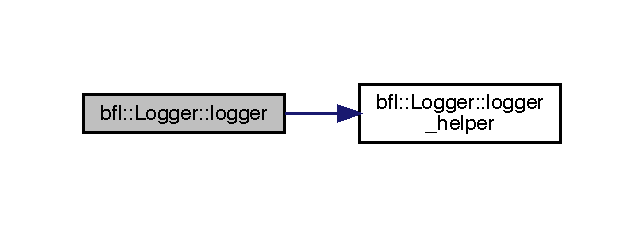
\includegraphics[width=309pt]{classbfl_1_1Logger_aca2086c9256e5c404872b91f7f25b97d_cgraph}
\end{center}
\end{figure}
\mbox{\Hypertarget{classbfl_1_1Logger_a50b1c109730fa98f66e66f420f0158fe}\label{classbfl_1_1Logger_a50b1c109730fa98f66e66f420f0158fe}} 
\index{bfl\+::\+Additive\+Measurement\+Model@{bfl\+::\+Additive\+Measurement\+Model}!logger@{logger}}
\index{logger@{logger}!bfl\+::\+Additive\+Measurement\+Model@{bfl\+::\+Additive\+Measurement\+Model}}
\subsubsection{\texorpdfstring{logger()}{logger()}\hspace{0.1cm}{\footnotesize\ttfamily [3/4]}}
{\footnotesize\ttfamily template$<$typename Datum\+Type $>$ \\
void bfl\+::\+Logger\+::logger (\begin{DoxyParamCaption}\item[{Datum\+Type}]{datum }\end{DoxyParamCaption}) const\hspace{0.3cm}{\ttfamily [inline]}, {\ttfamily [inherited]}}



Definition at line 42 of file Logger.\+h.



References bfl\+::\+Logger\+::log\+\_\+enabled\+\_\+, and bfl\+::\+Logger\+::log\+\_\+files\+\_\+.

\mbox{\Hypertarget{classbfl_1_1Logger_a0f0cf7ce956546d94dfb1feb7cebf171}\label{classbfl_1_1Logger_a0f0cf7ce956546d94dfb1feb7cebf171}} 
\index{bfl\+::\+Additive\+Measurement\+Model@{bfl\+::\+Additive\+Measurement\+Model}!logger@{logger}}
\index{logger@{logger}!bfl\+::\+Additive\+Measurement\+Model@{bfl\+::\+Additive\+Measurement\+Model}}
\subsubsection{\texorpdfstring{logger()}{logger()}\hspace{0.1cm}{\footnotesize\ttfamily [4/4]}}
{\footnotesize\ttfamily template$<$typename... Data\+Type$>$ \\
void bfl\+::\+Logger\+::logger (\begin{DoxyParamCaption}\item[{Data\+Type...}]{data }\end{DoxyParamCaption}) const\hspace{0.3cm}{\ttfamily [inline]}, {\ttfamily [inherited]}}



Definition at line 49 of file Logger.\+h.



References bfl\+::\+Logger\+::log\+\_\+enabled\+\_\+, and bfl\+::\+Logger\+::logger\+\_\+helper().

Here is the call graph for this function\+:
\nopagebreak
\begin{figure}[H]
\begin{center}
\leavevmode
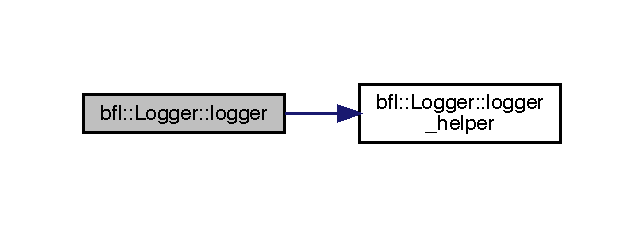
\includegraphics[width=309pt]{classbfl_1_1Logger_a0f0cf7ce956546d94dfb1feb7cebf171_cgraph}
\end{center}
\end{figure}
\mbox{\Hypertarget{classbfl_1_1MeasurementModel_ad372b720cef4e6bc0ac2489f4098bfc9}\label{classbfl_1_1MeasurementModel_ad372b720cef4e6bc0ac2489f4098bfc9}} 
\index{bfl\+::\+Additive\+Measurement\+Model@{bfl\+::\+Additive\+Measurement\+Model}!measure@{measure}}
\index{measure@{measure}!bfl\+::\+Additive\+Measurement\+Model@{bfl\+::\+Additive\+Measurement\+Model}}
\subsubsection{\texorpdfstring{measure()}{measure()}}
{\footnotesize\ttfamily virtual std\+::pair$<$bool, \mbox{\hyperlink{namespacebfl_af6b103c6821db1b54452f776fdd9dd02}{bfl\+::\+Data}}$>$ bfl\+::\+Measurement\+Model\+::measure (\begin{DoxyParamCaption}{ }\end{DoxyParamCaption}) const\hspace{0.3cm}{\ttfamily [pure virtual]}, {\ttfamily [inherited]}}



Implemented in \mbox{\hyperlink{classbfl_1_1SimulatedLinearSensor_a61c278bdbc5f3a0201d2f855a739d4f4}{bfl\+::\+Simulated\+Linear\+Sensor}}, and \mbox{\hyperlink{classbfl_1_1MeasurementModelDecorator_a36194c2f6abd7e13a417c3663febe921}{bfl\+::\+Measurement\+Model\+Decorator}}.



Referenced by bfl\+::\+U\+K\+F\+Correction\+::correct\+Step(), and bfl\+::\+Gaussian\+Likelihood\+::likelihood().

\mbox{\Hypertarget{classbfl_1_1MeasurementModel_a8fc8798aa2db48f428d4ce59b33b5307}\label{classbfl_1_1MeasurementModel_a8fc8798aa2db48f428d4ce59b33b5307}} 
\index{bfl\+::\+Additive\+Measurement\+Model@{bfl\+::\+Additive\+Measurement\+Model}!predicted\+Measure@{predicted\+Measure}}
\index{predicted\+Measure@{predicted\+Measure}!bfl\+::\+Additive\+Measurement\+Model@{bfl\+::\+Additive\+Measurement\+Model}}
\subsubsection{\texorpdfstring{predicted\+Measure()}{predictedMeasure()}}
{\footnotesize\ttfamily virtual std\+::pair$<$bool, \mbox{\hyperlink{namespacebfl_af6b103c6821db1b54452f776fdd9dd02}{bfl\+::\+Data}}$>$ bfl\+::\+Measurement\+Model\+::predicted\+Measure (\begin{DoxyParamCaption}\item[{const Eigen\+::\+Ref$<$ const Eigen\+::\+Matrix\+Xd $>$ \&}]{cur\+\_\+states }\end{DoxyParamCaption}) const\hspace{0.3cm}{\ttfamily [pure virtual]}, {\ttfamily [inherited]}}



Implemented in \mbox{\hyperlink{classbfl_1_1LinearMeasurementModel_a8831b8acb4790db4c69db73200375c69}{bfl\+::\+Linear\+Measurement\+Model}}, and \mbox{\hyperlink{classbfl_1_1MeasurementModelDecorator_ae4b5f665c511cb0fddaaf0a3de402f22}{bfl\+::\+Measurement\+Model\+Decorator}}.



Referenced by bfl\+::\+Gaussian\+Likelihood\+::likelihood(), and bfl\+::sigma\+\_\+point\+::unscented\+\_\+transform().

\mbox{\Hypertarget{classbfl_1_1MeasurementModel_af97e18b52d1a3f365dd5982b8cc4aff7}\label{classbfl_1_1MeasurementModel_af97e18b52d1a3f365dd5982b8cc4aff7}} 
\index{bfl\+::\+Additive\+Measurement\+Model@{bfl\+::\+Additive\+Measurement\+Model}!set\+Property@{set\+Property}}
\index{set\+Property@{set\+Property}!bfl\+::\+Additive\+Measurement\+Model@{bfl\+::\+Additive\+Measurement\+Model}}
\subsubsection{\texorpdfstring{set\+Property()}{setProperty()}}
{\footnotesize\ttfamily bool Measurement\+Model\+::set\+Property (\begin{DoxyParamCaption}\item[{const std\+::string \&}]{property }\end{DoxyParamCaption})\hspace{0.3cm}{\ttfamily [virtual]}, {\ttfamily [inherited]}}



Reimplemented in \mbox{\hyperlink{classbfl_1_1MeasurementModelDecorator_a531a891152d7bf83e56370664d54f42f}{bfl\+::\+Measurement\+Model\+Decorator}}.



Definition at line 19 of file Measurement\+Model.\+cpp.



The documentation for this class was generated from the following files\+:\begin{DoxyCompactItemize}
\item 
/\+Users/\+Claudio/\+Git\+Hub/bayes-\/filters-\/lib/src/\+Bayes\+Filters/include/\+Bayes\+Filters/\mbox{\hyperlink{AdditiveMeasurementModel_8h}{Additive\+Measurement\+Model.\+h}}\item 
/\+Users/\+Claudio/\+Git\+Hub/bayes-\/filters-\/lib/src/\+Bayes\+Filters/src/\mbox{\hyperlink{AdditiveMeasurementModel_8cpp}{Additive\+Measurement\+Model.\+cpp}}\end{DoxyCompactItemize}

\hypertarget{classbfl_1_1AdditiveStateModel}{}\section{bfl\+:\+:Additive\+State\+Model Class Reference}
\label{classbfl_1_1AdditiveStateModel}\index{bfl\+::\+Additive\+State\+Model@{bfl\+::\+Additive\+State\+Model}}


{\ttfamily \#include $<$Additive\+State\+Model.\+h$>$}



Inheritance diagram for bfl\+:\+:Additive\+State\+Model\+:
\nopagebreak
\begin{figure}[H]
\begin{center}
\leavevmode
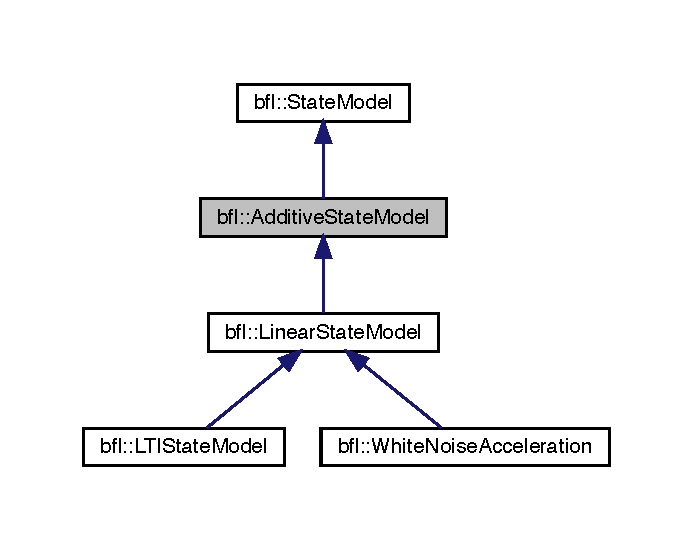
\includegraphics[width=332pt]{classbfl_1_1AdditiveStateModel__inherit__graph}
\end{center}
\end{figure}
\subsection*{Public Member Functions}
\begin{DoxyCompactItemize}
\item 
virtual \mbox{\hyperlink{classbfl_1_1AdditiveStateModel_a83769aadf851ecb2aef511dafd75e828}{$\sim$\+Additive\+State\+Model}} () noexcept
\item 
virtual void \mbox{\hyperlink{classbfl_1_1AdditiveStateModel_a9f145bf8c592fc0092d84421f26dbb8b}{motion}} (const Eigen\+::\+Ref$<$ const Eigen\+::\+Matrix\+Xd $>$ \&cur\+\_\+states, Eigen\+::\+Ref$<$ Eigen\+::\+Matrix\+Xd $>$ mot\+\_\+states) override
\item 
virtual void \mbox{\hyperlink{classbfl_1_1StateModel_a39cd8c8c5adbd623884583b4a7a7415c}{propagate}} (const Eigen\+::\+Ref$<$ const Eigen\+::\+Matrix\+Xd $>$ \&cur\+\_\+states, Eigen\+::\+Ref$<$ Eigen\+::\+Matrix\+Xd $>$ prop\+\_\+states)=0
\item 
virtual Eigen\+::\+Matrix\+Xd \mbox{\hyperlink{classbfl_1_1StateModel_a78df4b39578345142fcfb18abaab2177}{get\+Jacobian}} ()
\item 
virtual Eigen\+::\+Vector\+Xd \mbox{\hyperlink{classbfl_1_1StateModel_acb582cb7d41ec7b854ed1dbd8965b6fc}{get\+Transition\+Probability}} (const Eigen\+::\+Ref$<$ const Eigen\+::\+Matrix\+Xd $>$ \&prev\+\_\+states, Eigen\+::\+Ref$<$ Eigen\+::\+Matrix\+Xd $>$ cur\+\_\+states)
\item 
virtual Eigen\+::\+Matrix\+Xd \mbox{\hyperlink{classbfl_1_1StateModel_a423c1fa86b9d60c8663dedc6cdcae276}{get\+Noise\+Covariance\+Matrix}} ()
\item 
virtual Eigen\+::\+Matrix\+Xd \mbox{\hyperlink{classbfl_1_1StateModel_acc6733af2dcba2a330bf7c59c3725e42}{get\+Noise\+Sample}} (const std\+::size\+\_\+t num)
\item 
virtual bool \mbox{\hyperlink{classbfl_1_1StateModel_ac86dcdad8f0bbfab39a23e592779feaa}{set\+Property}} (const std\+::string \&property)=0
\item 
virtual std\+::pair$<$ std\+::size\+\_\+t, std\+::size\+\_\+t $>$ \mbox{\hyperlink{classbfl_1_1StateModel_a6bf680b689389d959fc9ac46595e6dab}{get\+Output\+Size}} () const =0
\begin{DoxyCompactList}\small\item\em Returns the linear and circular size of the output of the state equation. \end{DoxyCompactList}\end{DoxyCompactItemize}


\subsection{Detailed Description}


Definition at line 13 of file Additive\+State\+Model.\+h.



\subsection{Constructor \& Destructor Documentation}
\mbox{\Hypertarget{classbfl_1_1AdditiveStateModel_a83769aadf851ecb2aef511dafd75e828}\label{classbfl_1_1AdditiveStateModel_a83769aadf851ecb2aef511dafd75e828}} 
\index{bfl\+::\+Additive\+State\+Model@{bfl\+::\+Additive\+State\+Model}!````~Additive\+State\+Model@{$\sim$\+Additive\+State\+Model}}
\index{````~Additive\+State\+Model@{$\sim$\+Additive\+State\+Model}!bfl\+::\+Additive\+State\+Model@{bfl\+::\+Additive\+State\+Model}}
\subsubsection{\texorpdfstring{$\sim$\+Additive\+State\+Model()}{~AdditiveStateModel()}}
{\footnotesize\ttfamily virtual bfl\+::\+Additive\+State\+Model\+::$\sim$\+Additive\+State\+Model (\begin{DoxyParamCaption}{ }\end{DoxyParamCaption})\hspace{0.3cm}{\ttfamily [inline]}, {\ttfamily [virtual]}, {\ttfamily [noexcept]}}



Definition at line 16 of file Additive\+State\+Model.\+h.



\subsection{Member Function Documentation}
\mbox{\Hypertarget{classbfl_1_1StateModel_a78df4b39578345142fcfb18abaab2177}\label{classbfl_1_1StateModel_a78df4b39578345142fcfb18abaab2177}} 
\index{bfl\+::\+Additive\+State\+Model@{bfl\+::\+Additive\+State\+Model}!get\+Jacobian@{get\+Jacobian}}
\index{get\+Jacobian@{get\+Jacobian}!bfl\+::\+Additive\+State\+Model@{bfl\+::\+Additive\+State\+Model}}
\subsubsection{\texorpdfstring{get\+Jacobian()}{getJacobian()}}
{\footnotesize\ttfamily Eigen\+::\+Matrix\+Xd State\+Model\+::get\+Jacobian (\begin{DoxyParamCaption}{ }\end{DoxyParamCaption})\hspace{0.3cm}{\ttfamily [virtual]}, {\ttfamily [inherited]}}



Reimplemented in \mbox{\hyperlink{classbfl_1_1LTIStateModel_a5bdef1421c100bce7baa1961d2916fc3}{bfl\+::\+L\+T\+I\+State\+Model}}.



Definition at line 7 of file State\+Model.\+cpp.

\mbox{\Hypertarget{classbfl_1_1StateModel_a423c1fa86b9d60c8663dedc6cdcae276}\label{classbfl_1_1StateModel_a423c1fa86b9d60c8663dedc6cdcae276}} 
\index{bfl\+::\+Additive\+State\+Model@{bfl\+::\+Additive\+State\+Model}!get\+Noise\+Covariance\+Matrix@{get\+Noise\+Covariance\+Matrix}}
\index{get\+Noise\+Covariance\+Matrix@{get\+Noise\+Covariance\+Matrix}!bfl\+::\+Additive\+State\+Model@{bfl\+::\+Additive\+State\+Model}}
\subsubsection{\texorpdfstring{get\+Noise\+Covariance\+Matrix()}{getNoiseCovarianceMatrix()}}
{\footnotesize\ttfamily Eigen\+::\+Matrix\+Xd State\+Model\+::get\+Noise\+Covariance\+Matrix (\begin{DoxyParamCaption}{ }\end{DoxyParamCaption})\hspace{0.3cm}{\ttfamily [virtual]}, {\ttfamily [inherited]}}



Reimplemented in \mbox{\hyperlink{classbfl_1_1WhiteNoiseAcceleration_a453df5960973059b35ee8686dc12ab0d}{bfl\+::\+White\+Noise\+Acceleration}}, \mbox{\hyperlink{classbfl_1_1LTIStateModel_a60a5ab5f3013b771ddd73787edd8dcde}{bfl\+::\+L\+T\+I\+State\+Model}}, and \mbox{\hyperlink{classbfl_1_1StateModelDecorator_ae70700c1fad6b788b21722e57f2d0f6b}{bfl\+::\+State\+Model\+Decorator}}.



Definition at line 19 of file State\+Model.\+cpp.



Referenced by bfl\+::sigma\+\_\+point\+::unscented\+\_\+transform().

\mbox{\Hypertarget{classbfl_1_1StateModel_acc6733af2dcba2a330bf7c59c3725e42}\label{classbfl_1_1StateModel_acc6733af2dcba2a330bf7c59c3725e42}} 
\index{bfl\+::\+Additive\+State\+Model@{bfl\+::\+Additive\+State\+Model}!get\+Noise\+Sample@{get\+Noise\+Sample}}
\index{get\+Noise\+Sample@{get\+Noise\+Sample}!bfl\+::\+Additive\+State\+Model@{bfl\+::\+Additive\+State\+Model}}
\subsubsection{\texorpdfstring{get\+Noise\+Sample()}{getNoiseSample()}}
{\footnotesize\ttfamily Eigen\+::\+Matrix\+Xd State\+Model\+::get\+Noise\+Sample (\begin{DoxyParamCaption}\item[{const std\+::size\+\_\+t}]{num }\end{DoxyParamCaption})\hspace{0.3cm}{\ttfamily [virtual]}, {\ttfamily [inherited]}}



Reimplemented in \mbox{\hyperlink{classbfl_1_1WhiteNoiseAcceleration_a819bd0d5510c9863272b422ab33b7adc}{bfl\+::\+White\+Noise\+Acceleration}}, and \mbox{\hyperlink{classbfl_1_1StateModelDecorator_a6825b807be82c66feb8bbb62d240490b}{bfl\+::\+State\+Model\+Decorator}}.



Definition at line 25 of file State\+Model.\+cpp.

\mbox{\Hypertarget{classbfl_1_1StateModel_a6bf680b689389d959fc9ac46595e6dab}\label{classbfl_1_1StateModel_a6bf680b689389d959fc9ac46595e6dab}} 
\index{bfl\+::\+Additive\+State\+Model@{bfl\+::\+Additive\+State\+Model}!get\+Output\+Size@{get\+Output\+Size}}
\index{get\+Output\+Size@{get\+Output\+Size}!bfl\+::\+Additive\+State\+Model@{bfl\+::\+Additive\+State\+Model}}
\subsubsection{\texorpdfstring{get\+Output\+Size()}{getOutputSize()}}
{\footnotesize\ttfamily virtual std\+::pair$<$std\+::size\+\_\+t, std\+::size\+\_\+t$>$ bfl\+::\+State\+Model\+::get\+Output\+Size (\begin{DoxyParamCaption}{ }\end{DoxyParamCaption}) const\hspace{0.3cm}{\ttfamily [pure virtual]}, {\ttfamily [inherited]}}



Returns the linear and circular size of the output of the state equation. 



Implemented in \mbox{\hyperlink{classbfl_1_1WhiteNoiseAcceleration_ac3e447bf2f520b543c67d066f72423b7}{bfl\+::\+White\+Noise\+Acceleration}}, and \mbox{\hyperlink{classbfl_1_1StateModelDecorator_a2b2f00e6825e382587a2edbbba4569de}{bfl\+::\+State\+Model\+Decorator}}.



Referenced by bfl\+::sigma\+\_\+point\+::unscented\+\_\+transform().

\mbox{\Hypertarget{classbfl_1_1StateModel_acb582cb7d41ec7b854ed1dbd8965b6fc}\label{classbfl_1_1StateModel_acb582cb7d41ec7b854ed1dbd8965b6fc}} 
\index{bfl\+::\+Additive\+State\+Model@{bfl\+::\+Additive\+State\+Model}!get\+Transition\+Probability@{get\+Transition\+Probability}}
\index{get\+Transition\+Probability@{get\+Transition\+Probability}!bfl\+::\+Additive\+State\+Model@{bfl\+::\+Additive\+State\+Model}}
\subsubsection{\texorpdfstring{get\+Transition\+Probability()}{getTransitionProbability()}}
{\footnotesize\ttfamily Eigen\+::\+Vector\+Xd State\+Model\+::get\+Transition\+Probability (\begin{DoxyParamCaption}\item[{const Eigen\+::\+Ref$<$ const Eigen\+::\+Matrix\+Xd $>$ \&}]{prev\+\_\+states,  }\item[{Eigen\+::\+Ref$<$ Eigen\+::\+Matrix\+Xd $>$}]{cur\+\_\+states }\end{DoxyParamCaption})\hspace{0.3cm}{\ttfamily [virtual]}, {\ttfamily [inherited]}}



Reimplemented in \mbox{\hyperlink{classbfl_1_1WhiteNoiseAcceleration_a10d81273e59d14f7d7ce794533c122a8}{bfl\+::\+White\+Noise\+Acceleration}}.



Definition at line 13 of file State\+Model.\+cpp.

\mbox{\Hypertarget{classbfl_1_1AdditiveStateModel_a9f145bf8c592fc0092d84421f26dbb8b}\label{classbfl_1_1AdditiveStateModel_a9f145bf8c592fc0092d84421f26dbb8b}} 
\index{bfl\+::\+Additive\+State\+Model@{bfl\+::\+Additive\+State\+Model}!motion@{motion}}
\index{motion@{motion}!bfl\+::\+Additive\+State\+Model@{bfl\+::\+Additive\+State\+Model}}
\subsubsection{\texorpdfstring{motion()}{motion()}}
{\footnotesize\ttfamily void Additive\+State\+Model\+::motion (\begin{DoxyParamCaption}\item[{const Eigen\+::\+Ref$<$ const Eigen\+::\+Matrix\+Xd $>$ \&}]{cur\+\_\+states,  }\item[{Eigen\+::\+Ref$<$ Eigen\+::\+Matrix\+Xd $>$}]{mot\+\_\+states }\end{DoxyParamCaption})\hspace{0.3cm}{\ttfamily [override]}, {\ttfamily [virtual]}}



Implements \mbox{\hyperlink{classbfl_1_1StateModel_a34037bc30bc07667b76b5a719a65ab82}{bfl\+::\+State\+Model}}.



Definition at line 8 of file Additive\+State\+Model.\+cpp.

\mbox{\Hypertarget{classbfl_1_1StateModel_a39cd8c8c5adbd623884583b4a7a7415c}\label{classbfl_1_1StateModel_a39cd8c8c5adbd623884583b4a7a7415c}} 
\index{bfl\+::\+Additive\+State\+Model@{bfl\+::\+Additive\+State\+Model}!propagate@{propagate}}
\index{propagate@{propagate}!bfl\+::\+Additive\+State\+Model@{bfl\+::\+Additive\+State\+Model}}
\subsubsection{\texorpdfstring{propagate()}{propagate()}}
{\footnotesize\ttfamily virtual void bfl\+::\+State\+Model\+::propagate (\begin{DoxyParamCaption}\item[{const Eigen\+::\+Ref$<$ const Eigen\+::\+Matrix\+Xd $>$ \&}]{cur\+\_\+states,  }\item[{Eigen\+::\+Ref$<$ Eigen\+::\+Matrix\+Xd $>$}]{prop\+\_\+states }\end{DoxyParamCaption})\hspace{0.3cm}{\ttfamily [pure virtual]}, {\ttfamily [inherited]}}



Implemented in \mbox{\hyperlink{classbfl_1_1LTIStateModel_a0a736ef66903c2e598f0b86892a716aa}{bfl\+::\+L\+T\+I\+State\+Model}}, \mbox{\hyperlink{classbfl_1_1LinearStateModel_a7823383ddc1ed709b9399c712997f512}{bfl\+::\+Linear\+State\+Model}}, and \mbox{\hyperlink{classbfl_1_1StateModelDecorator_a9548415d6445c58778eeeadf48ff2672}{bfl\+::\+State\+Model\+Decorator}}.



Referenced by bfl\+::sigma\+\_\+point\+::unscented\+\_\+transform().

\mbox{\Hypertarget{classbfl_1_1StateModel_ac86dcdad8f0bbfab39a23e592779feaa}\label{classbfl_1_1StateModel_ac86dcdad8f0bbfab39a23e592779feaa}} 
\index{bfl\+::\+Additive\+State\+Model@{bfl\+::\+Additive\+State\+Model}!set\+Property@{set\+Property}}
\index{set\+Property@{set\+Property}!bfl\+::\+Additive\+State\+Model@{bfl\+::\+Additive\+State\+Model}}
\subsubsection{\texorpdfstring{set\+Property()}{setProperty()}}
{\footnotesize\ttfamily virtual bool bfl\+::\+State\+Model\+::set\+Property (\begin{DoxyParamCaption}\item[{const std\+::string \&}]{property }\end{DoxyParamCaption})\hspace{0.3cm}{\ttfamily [pure virtual]}, {\ttfamily [inherited]}}



Implemented in \mbox{\hyperlink{classbfl_1_1WhiteNoiseAcceleration_a0203b47074e0680852f53dcba8a7a627}{bfl\+::\+White\+Noise\+Acceleration}}, \mbox{\hyperlink{classbfl_1_1LTIStateModel_afc2264780111fe41b6a82e97bcb5e87c}{bfl\+::\+L\+T\+I\+State\+Model}}, and \mbox{\hyperlink{classbfl_1_1StateModelDecorator_ad292f3b665c1adf20a1f32dc8a065fec}{bfl\+::\+State\+Model\+Decorator}}.



The documentation for this class was generated from the following files\+:\begin{DoxyCompactItemize}
\item 
/\+Users/\+Claudio/\+Git\+Hub/bayes-\/filters-\/lib/src/\+Bayes\+Filters/include/\+Bayes\+Filters/\mbox{\hyperlink{AdditiveStateModel_8h}{Additive\+State\+Model.\+h}}\item 
/\+Users/\+Claudio/\+Git\+Hub/bayes-\/filters-\/lib/src/\+Bayes\+Filters/src/\mbox{\hyperlink{AdditiveStateModel_8cpp}{Additive\+State\+Model.\+cpp}}\end{DoxyCompactItemize}

\hypertarget{classbfl_1_1Agent}{}\section{bfl\+:\+:Agent Class Reference}
\label{classbfl_1_1Agent}\index{bfl\+::\+Agent@{bfl\+::\+Agent}}


{\ttfamily \#include $<$Agent.\+h$>$}



Inheritance diagram for bfl\+:\+:Agent\+:
\nopagebreak
\begin{figure}[H]
\begin{center}
\leavevmode
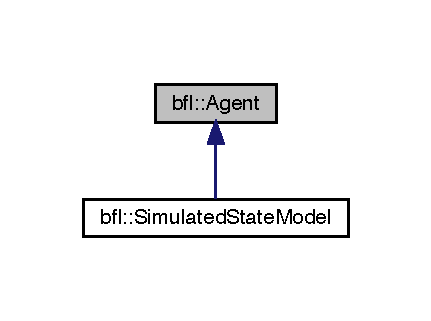
\includegraphics[width=207pt]{classbfl_1_1Agent__inherit__graph}
\end{center}
\end{figure}
\subsection*{Public Member Functions}
\begin{DoxyCompactItemize}
\item 
virtual \mbox{\hyperlink{classbfl_1_1Agent_acb45ed3a6892a9a66fdb37ad8e883428}{$\sim$\+Agent}} () noexcept
\item 
virtual bool \mbox{\hyperlink{classbfl_1_1Agent_aceb93f1712a98222af2b02537c09b6dc}{buffer\+Data}} ()=0
\item 
virtual \mbox{\hyperlink{namespacebfl_af6b103c6821db1b54452f776fdd9dd02}{Data}} \mbox{\hyperlink{classbfl_1_1Agent_a38522a865006e91ab426fe3bf3a6d4c8}{get\+Data}} () const =0
\item 
virtual bool \mbox{\hyperlink{classbfl_1_1Agent_a1291dcb438c8fc1400e1728711302007}{set\+Property}} (const std\+::string \&property)
\end{DoxyCompactItemize}


\subsection{Detailed Description}


Definition at line 16 of file Agent.\+h.



\subsection{Constructor \& Destructor Documentation}
\mbox{\Hypertarget{classbfl_1_1Agent_acb45ed3a6892a9a66fdb37ad8e883428}\label{classbfl_1_1Agent_acb45ed3a6892a9a66fdb37ad8e883428}} 
\index{bfl\+::\+Agent@{bfl\+::\+Agent}!````~Agent@{$\sim$\+Agent}}
\index{````~Agent@{$\sim$\+Agent}!bfl\+::\+Agent@{bfl\+::\+Agent}}
\subsubsection{\texorpdfstring{$\sim$\+Agent()}{~Agent()}}
{\footnotesize\ttfamily Agent\+::$\sim$\+Agent (\begin{DoxyParamCaption}{ }\end{DoxyParamCaption})\hspace{0.3cm}{\ttfamily [virtual]}, {\ttfamily [noexcept]}}



Definition at line 8 of file Agent.\+cpp.



\subsection{Member Function Documentation}
\mbox{\Hypertarget{classbfl_1_1Agent_aceb93f1712a98222af2b02537c09b6dc}\label{classbfl_1_1Agent_aceb93f1712a98222af2b02537c09b6dc}} 
\index{bfl\+::\+Agent@{bfl\+::\+Agent}!buffer\+Data@{buffer\+Data}}
\index{buffer\+Data@{buffer\+Data}!bfl\+::\+Agent@{bfl\+::\+Agent}}
\subsubsection{\texorpdfstring{buffer\+Data()}{bufferData()}}
{\footnotesize\ttfamily virtual bool bfl\+::\+Agent\+::buffer\+Data (\begin{DoxyParamCaption}{ }\end{DoxyParamCaption})\hspace{0.3cm}{\ttfamily [pure virtual]}}



Implemented in \mbox{\hyperlink{classbfl_1_1SimulatedStateModel_ae7bc3a9bf9d4ed8a8d1985772380295e}{bfl\+::\+Simulated\+State\+Model}}.

\mbox{\Hypertarget{classbfl_1_1Agent_a38522a865006e91ab426fe3bf3a6d4c8}\label{classbfl_1_1Agent_a38522a865006e91ab426fe3bf3a6d4c8}} 
\index{bfl\+::\+Agent@{bfl\+::\+Agent}!get\+Data@{get\+Data}}
\index{get\+Data@{get\+Data}!bfl\+::\+Agent@{bfl\+::\+Agent}}
\subsubsection{\texorpdfstring{get\+Data()}{getData()}}
{\footnotesize\ttfamily virtual \mbox{\hyperlink{namespacebfl_af6b103c6821db1b54452f776fdd9dd02}{Data}} bfl\+::\+Agent\+::get\+Data (\begin{DoxyParamCaption}{ }\end{DoxyParamCaption}) const\hspace{0.3cm}{\ttfamily [pure virtual]}}



Implemented in \mbox{\hyperlink{classbfl_1_1SimulatedStateModel_a23aa6df27179a9a48b48cf4002508ba9}{bfl\+::\+Simulated\+State\+Model}}.

\mbox{\Hypertarget{classbfl_1_1Agent_a1291dcb438c8fc1400e1728711302007}\label{classbfl_1_1Agent_a1291dcb438c8fc1400e1728711302007}} 
\index{bfl\+::\+Agent@{bfl\+::\+Agent}!set\+Property@{set\+Property}}
\index{set\+Property@{set\+Property}!bfl\+::\+Agent@{bfl\+::\+Agent}}
\subsubsection{\texorpdfstring{set\+Property()}{setProperty()}}
{\footnotesize\ttfamily bool Agent\+::set\+Property (\begin{DoxyParamCaption}\item[{const std\+::string \&}]{property }\end{DoxyParamCaption})\hspace{0.3cm}{\ttfamily [virtual]}}



Reimplemented in \mbox{\hyperlink{classbfl_1_1SimulatedStateModel_ab629cfc5e8db969760f5fa161a1cf360}{bfl\+::\+Simulated\+State\+Model}}.



Definition at line 12 of file Agent.\+cpp.



The documentation for this class was generated from the following files\+:\begin{DoxyCompactItemize}
\item 
/\+Users/\+Claudio/\+Git\+Hub/bayes-\/filters-\/lib/src/\+Bayes\+Filters/include/\+Bayes\+Filters/\mbox{\hyperlink{Agent_8h}{Agent.\+h}}\item 
/\+Users/\+Claudio/\+Git\+Hub/bayes-\/filters-\/lib/src/\+Bayes\+Filters/src/\mbox{\hyperlink{Agent_8cpp}{Agent.\+cpp}}\end{DoxyCompactItemize}

\hypertarget{classbfl_1_1any_1_1any}{}\section{bfl\+:\+:any\+:\+:any Class Reference}
\label{classbfl_1_1any_1_1any}\index{bfl\+::any\+::any@{bfl\+::any\+::any}}


The class any describes a type-\/safe container for single values of any type.  




{\ttfamily \#include $<$any.\+h$>$}

\subsection*{Classes}
\begin{DoxyCompactItemize}
\item 
class \mbox{\hyperlink{classbfl_1_1any_1_1any_1_1holder}{holder}}
\item 
class \mbox{\hyperlink{classbfl_1_1any_1_1any_1_1placeholder}{placeholder}}
\end{DoxyCompactItemize}
\subsection*{Public Member Functions}
\begin{DoxyCompactItemize}
\item 
\mbox{\hyperlink{classbfl_1_1any_1_1any_a55b5d940fdb6f1e7215332b7d97c6365}{any}} () noexcept
\begin{DoxyCompactList}\small\item\em Constructs an empty object. \end{DoxyCompactList}\item 
\mbox{\hyperlink{classbfl_1_1any_1_1any_a85f150e4daa7d447586df005cc8d9846}{any}} (const \mbox{\hyperlink{classbfl_1_1any_1_1any}{any}} \&other)
\begin{DoxyCompactList}\small\item\em Copies content of other into a new instance, so that any content is equivalent in both type and value to those of other prior to the constructor call, or empty if other is empty. \end{DoxyCompactList}\item 
\mbox{\hyperlink{classbfl_1_1any_1_1any_ab3caf90d0d0e9a57a9cacc690fa57bf5}{any}} (\mbox{\hyperlink{classbfl_1_1any_1_1any}{any}} \&\&other) noexcept
\begin{DoxyCompactList}\small\item\em Moves content of other into a new instance, so that any content is equivalent in both type and value to those of other prior to the constructor call, or empty if other is empty. \end{DoxyCompactList}\item 
{\footnotesize template$<$typename Value\+Type $>$ }\\\mbox{\hyperlink{classbfl_1_1any_1_1any_a71949c13d541881e9e61de1064710616}{any}} (const Value\+Type \&value)
\begin{DoxyCompactList}\small\item\em Constructs an object with initial content an object of type std\+::decay\+\_\+t$<$\+Value\+Type$>$, direct-\/initialized from std\+::forward$<$\+Value\+Type$>$(value). \end{DoxyCompactList}\item 
{\footnotesize template$<$typename Value\+Type $>$ }\\\mbox{\hyperlink{classbfl_1_1any_1_1any_acb42da22b210ada4113f26025548175c}{any}} (Value\+Type \&\&value, typename std\+::enable\+\_\+if$<$!std\+::is\+\_\+same$<$ \mbox{\hyperlink{classbfl_1_1any_1_1any}{any}} \&, Value\+Type $>$\+::value $>$\+::\mbox{\hyperlink{classbfl_1_1any_1_1any_ad84c3b30ce2ed9d04fe28465b60f2500}{type}} $\ast$=0, typename std\+::enable\+\_\+if$<$!std\+::is\+\_\+const$<$ Value\+Type $>$\+::value $>$\+::\mbox{\hyperlink{classbfl_1_1any_1_1any_ad84c3b30ce2ed9d04fe28465b60f2500}{type}} $\ast$=0)
\begin{DoxyCompactList}\small\item\em Constructs an object with initial content an object of type std\+::decay\+\_\+t$<$\+Value\+Type$>$, direct-\/initialized from std\+::forward$<$\+Value\+Type$>$(value). \end{DoxyCompactList}\item 
\mbox{\hyperlink{classbfl_1_1any_1_1any_a14390d38352d52e2a447dc62d0b19941}{$\sim$any}} () noexcept
\begin{DoxyCompactList}\small\item\em Destruct the object. \end{DoxyCompactList}\item 
\mbox{\hyperlink{classbfl_1_1any_1_1any}{any}} \& \mbox{\hyperlink{classbfl_1_1any_1_1any_a067d769bffdf2782e8d1dc080f66d948}{operator=}} (const \mbox{\hyperlink{classbfl_1_1any_1_1any}{any}} \&rhs)
\begin{DoxyCompactList}\small\item\em Assigns contents to the contained value. \end{DoxyCompactList}\item 
\mbox{\hyperlink{classbfl_1_1any_1_1any}{any}} \& \mbox{\hyperlink{classbfl_1_1any_1_1any_a65609849a81b0af40e6b86751ae0350c}{operator=}} (\mbox{\hyperlink{classbfl_1_1any_1_1any}{any}} \&\&rhs) noexcept
\begin{DoxyCompactList}\small\item\em Assigns contents to the contained value. \end{DoxyCompactList}\item 
{\footnotesize template$<$class Value\+Type $>$ }\\\mbox{\hyperlink{classbfl_1_1any_1_1any}{any}} \& \mbox{\hyperlink{classbfl_1_1any_1_1any_a62a6777ca18bd10bf05ffa0f6d131435}{operator=}} (Value\+Type \&\&rhs)
\begin{DoxyCompactList}\small\item\em Assigns contents to the contained value. \end{DoxyCompactList}\item 
void \mbox{\hyperlink{classbfl_1_1any_1_1any_ae4e063fb12711ea99a78bdab4d5c3e36}{reset}} () noexcept
\begin{DoxyCompactList}\small\item\em If not empty, destroys the contained object. \end{DoxyCompactList}\item 
\mbox{\hyperlink{classbfl_1_1any_1_1any}{any}} \& \mbox{\hyperlink{classbfl_1_1any_1_1any_a0441e5816aa5ef4721f134868b7ca402}{swap}} (\mbox{\hyperlink{classbfl_1_1any_1_1any}{any}} \&rhs) noexcept
\begin{DoxyCompactList}\small\item\em Swaps the content of two any objects. \end{DoxyCompactList}\item 
bool \mbox{\hyperlink{classbfl_1_1any_1_1any_a6ec222b8ae338c3392b0538ec1d94766}{has\+\_\+value}} () const noexcept
\begin{DoxyCompactList}\small\item\em Checks whether the object contains a value. \end{DoxyCompactList}\item 
const std\+::type\+\_\+info \& \mbox{\hyperlink{classbfl_1_1any_1_1any_ad84c3b30ce2ed9d04fe28465b60f2500}{type}} () const noexcept
\begin{DoxyCompactList}\small\item\em Queries the contained type. \end{DoxyCompactList}\end{DoxyCompactItemize}
\subsection*{Private Attributes}
\begin{DoxyCompactItemize}
\item 
\mbox{\hyperlink{classbfl_1_1any_1_1any_1_1placeholder}{placeholder}} $\ast$ \mbox{\hyperlink{classbfl_1_1any_1_1any_a3b81eea753ab84d245b0b360bcb38540}{content}}
\end{DoxyCompactItemize}
\subsection*{Friends}
\begin{DoxyCompactItemize}
\item 
{\footnotesize template$<$typename Value\+Type $>$ }\\Value\+Type $\ast$ \mbox{\hyperlink{classbfl_1_1any_1_1any_a9d1312e2ae8ed7cf8cc7c93d4c6d1422}{any\+\_\+cast}} (\mbox{\hyperlink{classbfl_1_1any_1_1any}{any}} $\ast$) noexcept
\begin{DoxyCompactList}\small\item\em Performs type-\/safe access to the contained object. \end{DoxyCompactList}\end{DoxyCompactItemize}


\subsection{Detailed Description}
The class any describes a type-\/safe container for single values of any type. 

An object of class any stores an instance of any type that satisfies the constructor requirements or is empty, and this is referred to as the state of the class any object. The stored instance is called the contained object. Two states are equivalent if they are either both empty or if both are not empty and if the contained objects are equivalent. The non-\/member any\+\_\+cast functions provide type-\/safe access to the contained object. 

Definition at line 75 of file any.\+h.



\subsection{Constructor \& Destructor Documentation}
\mbox{\Hypertarget{classbfl_1_1any_1_1any_a55b5d940fdb6f1e7215332b7d97c6365}\label{classbfl_1_1any_1_1any_a55b5d940fdb6f1e7215332b7d97c6365}} 
\index{bfl\+::any\+::any@{bfl\+::any\+::any}!any@{any}}
\index{any@{any}!bfl\+::any\+::any@{bfl\+::any\+::any}}
\subsubsection{\texorpdfstring{any()}{any()}\hspace{0.1cm}{\footnotesize\ttfamily [1/5]}}
{\footnotesize\ttfamily bfl\+::any\+::any\+::any (\begin{DoxyParamCaption}{ }\end{DoxyParamCaption})\hspace{0.3cm}{\ttfamily [inline]}, {\ttfamily [noexcept]}}



Constructs an empty object. 



Definition at line 81 of file any.\+h.



Referenced by operator=(), and reset().

\mbox{\Hypertarget{classbfl_1_1any_1_1any_a85f150e4daa7d447586df005cc8d9846}\label{classbfl_1_1any_1_1any_a85f150e4daa7d447586df005cc8d9846}} 
\index{bfl\+::any\+::any@{bfl\+::any\+::any}!any@{any}}
\index{any@{any}!bfl\+::any\+::any@{bfl\+::any\+::any}}
\subsubsection{\texorpdfstring{any()}{any()}\hspace{0.1cm}{\footnotesize\ttfamily [2/5]}}
{\footnotesize\ttfamily bfl\+::any\+::any\+::any (\begin{DoxyParamCaption}\item[{const \mbox{\hyperlink{classbfl_1_1any_1_1any}{any}} \&}]{other }\end{DoxyParamCaption})\hspace{0.3cm}{\ttfamily [inline]}}



Copies content of other into a new instance, so that any content is equivalent in both type and value to those of other prior to the constructor call, or empty if other is empty. 



Definition at line 91 of file any.\+h.

\mbox{\Hypertarget{classbfl_1_1any_1_1any_ab3caf90d0d0e9a57a9cacc690fa57bf5}\label{classbfl_1_1any_1_1any_ab3caf90d0d0e9a57a9cacc690fa57bf5}} 
\index{bfl\+::any\+::any@{bfl\+::any\+::any}!any@{any}}
\index{any@{any}!bfl\+::any\+::any@{bfl\+::any\+::any}}
\subsubsection{\texorpdfstring{any()}{any()}\hspace{0.1cm}{\footnotesize\ttfamily [3/5]}}
{\footnotesize\ttfamily bfl\+::any\+::any\+::any (\begin{DoxyParamCaption}\item[{\mbox{\hyperlink{classbfl_1_1any_1_1any}{any}} \&\&}]{other }\end{DoxyParamCaption})\hspace{0.3cm}{\ttfamily [inline]}, {\ttfamily [noexcept]}}



Moves content of other into a new instance, so that any content is equivalent in both type and value to those of other prior to the constructor call, or empty if other is empty. 



Definition at line 101 of file any.\+h.

\mbox{\Hypertarget{classbfl_1_1any_1_1any_a71949c13d541881e9e61de1064710616}\label{classbfl_1_1any_1_1any_a71949c13d541881e9e61de1064710616}} 
\index{bfl\+::any\+::any@{bfl\+::any\+::any}!any@{any}}
\index{any@{any}!bfl\+::any\+::any@{bfl\+::any\+::any}}
\subsubsection{\texorpdfstring{any()}{any()}\hspace{0.1cm}{\footnotesize\ttfamily [4/5]}}
{\footnotesize\ttfamily template$<$typename Value\+Type $>$ \\
bfl\+::any\+::any\+::any (\begin{DoxyParamCaption}\item[{const Value\+Type \&}]{value }\end{DoxyParamCaption})\hspace{0.3cm}{\ttfamily [inline]}}



Constructs an object with initial content an object of type std\+::decay\+\_\+t$<$\+Value\+Type$>$, direct-\/initialized from std\+::forward$<$\+Value\+Type$>$(value). 

If std\+::is\+\_\+copy\+\_\+constructible$<$std\+::decay\+\_\+t$<$\+Value\+Type$>$$>$\+::value is false, the program is ill-\/formed. 

Definition at line 114 of file any.\+h.

\mbox{\Hypertarget{classbfl_1_1any_1_1any_acb42da22b210ada4113f26025548175c}\label{classbfl_1_1any_1_1any_acb42da22b210ada4113f26025548175c}} 
\index{bfl\+::any\+::any@{bfl\+::any\+::any}!any@{any}}
\index{any@{any}!bfl\+::any\+::any@{bfl\+::any\+::any}}
\subsubsection{\texorpdfstring{any()}{any()}\hspace{0.1cm}{\footnotesize\ttfamily [5/5]}}
{\footnotesize\ttfamily template$<$typename Value\+Type $>$ \\
bfl\+::any\+::any\+::any (\begin{DoxyParamCaption}\item[{Value\+Type \&\&}]{value,  }\item[{typename std\+::enable\+\_\+if$<$!std\+::is\+\_\+same$<$ \mbox{\hyperlink{classbfl_1_1any_1_1any}{any}} \&, Value\+Type $>$\+::value $>$\+::\mbox{\hyperlink{classbfl_1_1any_1_1any_ad84c3b30ce2ed9d04fe28465b60f2500}{type}} $\ast$}]{ = {\ttfamily 0},  }\item[{typename std\+::enable\+\_\+if$<$!std\+::is\+\_\+const$<$ Value\+Type $>$\+::value $>$\+::\mbox{\hyperlink{classbfl_1_1any_1_1any_ad84c3b30ce2ed9d04fe28465b60f2500}{type}} $\ast$}]{ = {\ttfamily 0} }\end{DoxyParamCaption})\hspace{0.3cm}{\ttfamily [inline]}}



Constructs an object with initial content an object of type std\+::decay\+\_\+t$<$\+Value\+Type$>$, direct-\/initialized from std\+::forward$<$\+Value\+Type$>$(value). 

If std\+::is\+\_\+copy\+\_\+constructible$<$std\+::decay\+\_\+t$<$\+Value\+Type$>$$>$\+::value is false, the program is ill-\/formed. 

Definition at line 125 of file any.\+h.

\mbox{\Hypertarget{classbfl_1_1any_1_1any_a14390d38352d52e2a447dc62d0b19941}\label{classbfl_1_1any_1_1any_a14390d38352d52e2a447dc62d0b19941}} 
\index{bfl\+::any\+::any@{bfl\+::any\+::any}!````~any@{$\sim$any}}
\index{````~any@{$\sim$any}!bfl\+::any\+::any@{bfl\+::any\+::any}}
\subsubsection{\texorpdfstring{$\sim$any()}{~any()}}
{\footnotesize\ttfamily bfl\+::any\+::any\+::$\sim$any (\begin{DoxyParamCaption}{ }\end{DoxyParamCaption})\hspace{0.3cm}{\ttfamily [inline]}, {\ttfamily [noexcept]}}



Destruct the object. 



Definition at line 133 of file any.\+h.



References content.



\subsection{Member Function Documentation}
\mbox{\Hypertarget{classbfl_1_1any_1_1any_a6ec222b8ae338c3392b0538ec1d94766}\label{classbfl_1_1any_1_1any_a6ec222b8ae338c3392b0538ec1d94766}} 
\index{bfl\+::any\+::any@{bfl\+::any\+::any}!has\+\_\+value@{has\+\_\+value}}
\index{has\+\_\+value@{has\+\_\+value}!bfl\+::any\+::any@{bfl\+::any\+::any}}
\subsubsection{\texorpdfstring{has\+\_\+value()}{has\_value()}}
{\footnotesize\ttfamily bool bfl\+::any\+::any\+::has\+\_\+value (\begin{DoxyParamCaption}{ }\end{DoxyParamCaption}) const\hspace{0.3cm}{\ttfamily [inline]}, {\ttfamily [noexcept]}}



Checks whether the object contains a value. 

\begin{DoxyReturn}{Returns}
true if instance contains a value, otherwise false. 
\end{DoxyReturn}


Definition at line 208 of file any.\+h.



References content.

\mbox{\Hypertarget{classbfl_1_1any_1_1any_a067d769bffdf2782e8d1dc080f66d948}\label{classbfl_1_1any_1_1any_a067d769bffdf2782e8d1dc080f66d948}} 
\index{bfl\+::any\+::any@{bfl\+::any\+::any}!operator=@{operator=}}
\index{operator=@{operator=}!bfl\+::any\+::any@{bfl\+::any\+::any}}
\subsubsection{\texorpdfstring{operator=()}{operator=()}\hspace{0.1cm}{\footnotesize\ttfamily [1/3]}}
{\footnotesize\ttfamily \mbox{\hyperlink{classbfl_1_1any_1_1any}{any}}\& bfl\+::any\+::any\+::operator= (\begin{DoxyParamCaption}\item[{const \mbox{\hyperlink{classbfl_1_1any_1_1any}{any}} \&}]{rhs }\end{DoxyParamCaption})\hspace{0.3cm}{\ttfamily [inline]}}



Assigns contents to the contained value. 

Assigns by copying the state of rhs, as if by any(rhs).swap($\ast$this).


\begin{DoxyParams}{Parameters}
{\em rhs} & object whose contained value to assign \\
\hline
\end{DoxyParams}


Definition at line 145 of file any.\+h.



References any().

Here is the call graph for this function\+:
\nopagebreak
\begin{figure}[H]
\begin{center}
\leavevmode
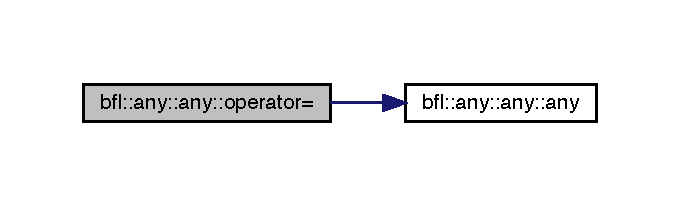
\includegraphics[width=326pt]{classbfl_1_1any_1_1any_a067d769bffdf2782e8d1dc080f66d948_cgraph}
\end{center}
\end{figure}
\mbox{\Hypertarget{classbfl_1_1any_1_1any_a65609849a81b0af40e6b86751ae0350c}\label{classbfl_1_1any_1_1any_a65609849a81b0af40e6b86751ae0350c}} 
\index{bfl\+::any\+::any@{bfl\+::any\+::any}!operator=@{operator=}}
\index{operator=@{operator=}!bfl\+::any\+::any@{bfl\+::any\+::any}}
\subsubsection{\texorpdfstring{operator=()}{operator=()}\hspace{0.1cm}{\footnotesize\ttfamily [2/3]}}
{\footnotesize\ttfamily \mbox{\hyperlink{classbfl_1_1any_1_1any}{any}}\& bfl\+::any\+::any\+::operator= (\begin{DoxyParamCaption}\item[{\mbox{\hyperlink{classbfl_1_1any_1_1any}{any}} \&\&}]{rhs }\end{DoxyParamCaption})\hspace{0.3cm}{\ttfamily [inline]}, {\ttfamily [noexcept]}}



Assigns contents to the contained value. 

Assigns by moving the state of rhs, as if by any(std\+::move(rhs)).swap($\ast$this). rhs is left in a valid but unspecified state after the assignment.


\begin{DoxyParams}{Parameters}
{\em rhs} & object whose contained value to assign \\
\hline
\end{DoxyParams}


Definition at line 159 of file any.\+h.



References any(), and swap().

Here is the call graph for this function\+:
\nopagebreak
\begin{figure}[H]
\begin{center}
\leavevmode
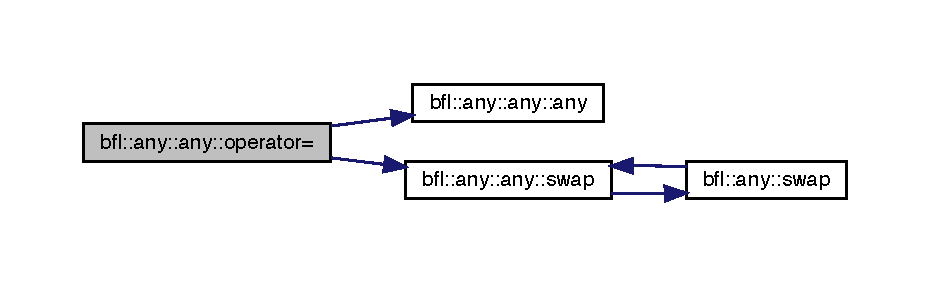
\includegraphics[width=350pt]{classbfl_1_1any_1_1any_a65609849a81b0af40e6b86751ae0350c_cgraph}
\end{center}
\end{figure}
\mbox{\Hypertarget{classbfl_1_1any_1_1any_a62a6777ca18bd10bf05ffa0f6d131435}\label{classbfl_1_1any_1_1any_a62a6777ca18bd10bf05ffa0f6d131435}} 
\index{bfl\+::any\+::any@{bfl\+::any\+::any}!operator=@{operator=}}
\index{operator=@{operator=}!bfl\+::any\+::any@{bfl\+::any\+::any}}
\subsubsection{\texorpdfstring{operator=()}{operator=()}\hspace{0.1cm}{\footnotesize\ttfamily [3/3]}}
{\footnotesize\ttfamily template$<$class Value\+Type $>$ \\
\mbox{\hyperlink{classbfl_1_1any_1_1any}{any}}\& bfl\+::any\+::any\+::operator= (\begin{DoxyParamCaption}\item[{Value\+Type \&\&}]{rhs }\end{DoxyParamCaption})\hspace{0.3cm}{\ttfamily [inline]}}



Assigns contents to the contained value. 

Assigns the type and value of rhs, as if by any(std\+::forward$<$\+Value\+Type$>$(rhs)).swap($\ast$this). This overload only participates in overload resolution if std\+::decay\+\_\+t$<$\+Value\+Type$>$ is not the same type as any and std\+::is\+\_\+copy\+\_\+constructible\+\_\+v$<$std\+::decay\+\_\+t$<$\+Value\+Type$>$$>$ is true.


\begin{DoxyParams}{Parameters}
{\em rhs} & object whose contained value to assign \\
\hline
\end{DoxyParams}


Definition at line 176 of file any.\+h.



References any().

Here is the call graph for this function\+:
\nopagebreak
\begin{figure}[H]
\begin{center}
\leavevmode
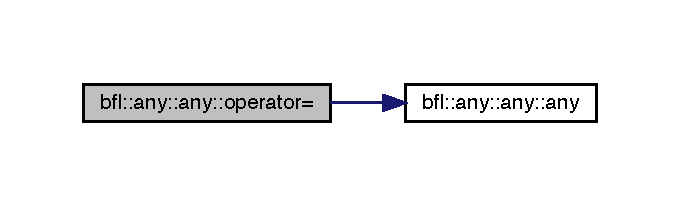
\includegraphics[width=326pt]{classbfl_1_1any_1_1any_a62a6777ca18bd10bf05ffa0f6d131435_cgraph}
\end{center}
\end{figure}
\mbox{\Hypertarget{classbfl_1_1any_1_1any_ae4e063fb12711ea99a78bdab4d5c3e36}\label{classbfl_1_1any_1_1any_ae4e063fb12711ea99a78bdab4d5c3e36}} 
\index{bfl\+::any\+::any@{bfl\+::any\+::any}!reset@{reset}}
\index{reset@{reset}!bfl\+::any\+::any@{bfl\+::any\+::any}}
\subsubsection{\texorpdfstring{reset()}{reset()}}
{\footnotesize\ttfamily void bfl\+::any\+::any\+::reset (\begin{DoxyParamCaption}{ }\end{DoxyParamCaption})\hspace{0.3cm}{\ttfamily [inline]}, {\ttfamily [noexcept]}}



If not empty, destroys the contained object. 



Definition at line 186 of file any.\+h.



References any().

Here is the call graph for this function\+:
\nopagebreak
\begin{figure}[H]
\begin{center}
\leavevmode
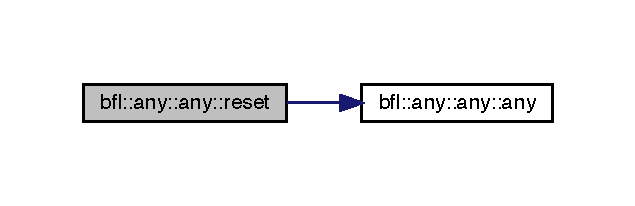
\includegraphics[width=305pt]{classbfl_1_1any_1_1any_ae4e063fb12711ea99a78bdab4d5c3e36_cgraph}
\end{center}
\end{figure}
\mbox{\Hypertarget{classbfl_1_1any_1_1any_a0441e5816aa5ef4721f134868b7ca402}\label{classbfl_1_1any_1_1any_a0441e5816aa5ef4721f134868b7ca402}} 
\index{bfl\+::any\+::any@{bfl\+::any\+::any}!swap@{swap}}
\index{swap@{swap}!bfl\+::any\+::any@{bfl\+::any\+::any}}
\subsubsection{\texorpdfstring{swap()}{swap()}}
{\footnotesize\ttfamily \mbox{\hyperlink{classbfl_1_1any_1_1any}{any}}\& bfl\+::any\+::any\+::swap (\begin{DoxyParamCaption}\item[{\mbox{\hyperlink{classbfl_1_1any_1_1any}{any}} \&}]{rhs }\end{DoxyParamCaption})\hspace{0.3cm}{\ttfamily [inline]}, {\ttfamily [noexcept]}}



Swaps the content of two any objects. 


\begin{DoxyParams}{Parameters}
{\em other} & object to swap with \\
\hline
\end{DoxyParams}


Definition at line 197 of file any.\+h.



References content, and bfl\+::any\+::swap().



Referenced by operator=(), and bfl\+::any\+::swap().

Here is the call graph for this function\+:
\nopagebreak
\begin{figure}[H]
\begin{center}
\leavevmode
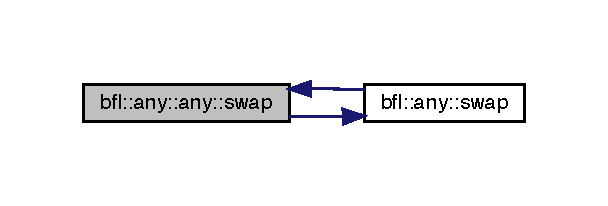
\includegraphics[width=292pt]{classbfl_1_1any_1_1any_a0441e5816aa5ef4721f134868b7ca402_cgraph}
\end{center}
\end{figure}
\mbox{\Hypertarget{classbfl_1_1any_1_1any_ad84c3b30ce2ed9d04fe28465b60f2500}\label{classbfl_1_1any_1_1any_ad84c3b30ce2ed9d04fe28465b60f2500}} 
\index{bfl\+::any\+::any@{bfl\+::any\+::any}!type@{type}}
\index{type@{type}!bfl\+::any\+::any@{bfl\+::any\+::any}}
\subsubsection{\texorpdfstring{type()}{type()}}
{\footnotesize\ttfamily const std\+::type\+\_\+info\& bfl\+::any\+::any\+::type (\begin{DoxyParamCaption}{ }\end{DoxyParamCaption}) const\hspace{0.3cm}{\ttfamily [inline]}, {\ttfamily [noexcept]}}



Queries the contained type. 

The typeid of the contained value if instance is non-\/empty, otherwise typeid(void). 

Definition at line 219 of file any.\+h.



References content, and bfl\+::any\+::any\+::placeholder\+::type().



Referenced by bfl\+::any\+::any\+\_\+cast().

Here is the call graph for this function\+:
\nopagebreak
\begin{figure}[H]
\begin{center}
\leavevmode
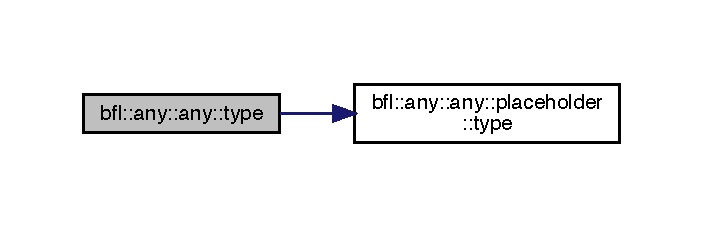
\includegraphics[width=338pt]{classbfl_1_1any_1_1any_ad84c3b30ce2ed9d04fe28465b60f2500_cgraph}
\end{center}
\end{figure}


\subsection{Friends And Related Function Documentation}
\mbox{\Hypertarget{classbfl_1_1any_1_1any_a9d1312e2ae8ed7cf8cc7c93d4c6d1422}\label{classbfl_1_1any_1_1any_a9d1312e2ae8ed7cf8cc7c93d4c6d1422}} 
\index{bfl\+::any\+::any@{bfl\+::any\+::any}!any\+\_\+cast@{any\+\_\+cast}}
\index{any\+\_\+cast@{any\+\_\+cast}!bfl\+::any\+::any@{bfl\+::any\+::any}}
\subsubsection{\texorpdfstring{any\+\_\+cast}{any\_cast}}
{\footnotesize\ttfamily template$<$typename Value\+Type $>$ \\
Value\+Type$\ast$ any\+\_\+cast (\begin{DoxyParamCaption}\item[{\mbox{\hyperlink{classbfl_1_1any_1_1any}{any}} $\ast$}]{operand }\end{DoxyParamCaption})\hspace{0.3cm}{\ttfamily [friend]}}



Performs type-\/safe access to the contained object. 

Throws libanyboost\+::bad\+\_\+any\+\_\+cast if the typeid of the requested Value\+Type does not match that of the contents of operand.


\begin{DoxyParams}{Parameters}
{\em operand} & target any object \\
\hline
\end{DoxyParams}


Definition at line 322 of file any.\+h.



Referenced by bfl\+::any\+::any\+\_\+cast().



\subsection{Member Data Documentation}
\mbox{\Hypertarget{classbfl_1_1any_1_1any_a3b81eea753ab84d245b0b360bcb38540}\label{classbfl_1_1any_1_1any_a3b81eea753ab84d245b0b360bcb38540}} 
\index{bfl\+::any\+::any@{bfl\+::any\+::any}!content@{content}}
\index{content@{content}!bfl\+::any\+::any@{bfl\+::any\+::any}}
\subsubsection{\texorpdfstring{content}{content}}
{\footnotesize\ttfamily \mbox{\hyperlink{classbfl_1_1any_1_1any_1_1placeholder}{placeholder}}$\ast$ bfl\+::any\+::any\+::content\hspace{0.3cm}{\ttfamily [private]}}



Definition at line 277 of file any.\+h.



Referenced by has\+\_\+value(), swap(), type(), and $\sim$any().



The documentation for this class was generated from the following file\+:\begin{DoxyCompactItemize}
\item 
/\+Users/\+Claudio/\+Git\+Hub/bayes-\/filters-\/lib/src/\+Bayes\+Filters/include/\+Bayes\+Filters/\mbox{\hyperlink{any_8h}{any.\+h}}\end{DoxyCompactItemize}

\hypertarget{classbfl_1_1any_1_1bad__any__cast}{}\section{bfl\+:\+:any\+:\+:bad\+\_\+any\+\_\+cast Class Reference}
\label{classbfl_1_1any_1_1bad__any__cast}\index{bfl\+::any\+::bad\+\_\+any\+\_\+cast@{bfl\+::any\+::bad\+\_\+any\+\_\+cast}}


Defines a type of object to be thrown by the value-\/returning forms of libanyboost\+::any\+\_\+cast on failure.  




{\ttfamily \#include $<$any.\+h$>$}



Inheritance diagram for bfl\+:\+:any\+:\+:bad\+\_\+any\+\_\+cast\+:
\nopagebreak
\begin{figure}[H]
\begin{center}
\leavevmode
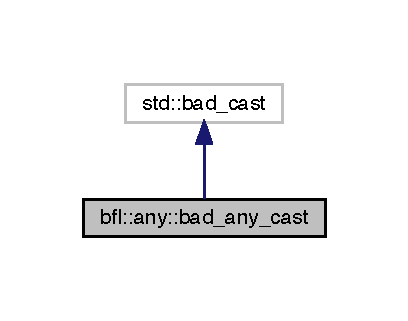
\includegraphics[width=196pt]{classbfl_1_1any_1_1bad__any__cast__inherit__graph}
\end{center}
\end{figure}
\subsection*{Public Member Functions}
\begin{DoxyCompactItemize}
\item 
virtual const char $\ast$ \mbox{\hyperlink{classbfl_1_1any_1_1bad__any__cast_a5e59fa8f7c57b8a06fb35bf66dd887eb}{what}} () const noexcept override
\begin{DoxyCompactList}\small\item\em Returns the explanatory string. \end{DoxyCompactList}\end{DoxyCompactItemize}


\subsection{Detailed Description}
Defines a type of object to be thrown by the value-\/returning forms of libanyboost\+::any\+\_\+cast on failure. 

Definition at line 296 of file any.\+h.



\subsection{Member Function Documentation}
\mbox{\Hypertarget{classbfl_1_1any_1_1bad__any__cast_a5e59fa8f7c57b8a06fb35bf66dd887eb}\label{classbfl_1_1any_1_1bad__any__cast_a5e59fa8f7c57b8a06fb35bf66dd887eb}} 
\index{bfl\+::any\+::bad\+\_\+any\+\_\+cast@{bfl\+::any\+::bad\+\_\+any\+\_\+cast}!what@{what}}
\index{what@{what}!bfl\+::any\+::bad\+\_\+any\+\_\+cast@{bfl\+::any\+::bad\+\_\+any\+\_\+cast}}
\subsubsection{\texorpdfstring{what()}{what()}}
{\footnotesize\ttfamily virtual const char$\ast$ bfl\+::any\+::bad\+\_\+any\+\_\+cast\+::what (\begin{DoxyParamCaption}{ }\end{DoxyParamCaption}) const\hspace{0.3cm}{\ttfamily [inline]}, {\ttfamily [override]}, {\ttfamily [virtual]}, {\ttfamily [noexcept]}}



Returns the explanatory string. 

Pointer to a null-\/terminated string with explanatory information. The pointer is guaranteed to be valid at least until the exception object from which it is obtained is destroyed, or until a non-\/const member function on the exception object is called. 

Definition at line 306 of file any.\+h.



The documentation for this class was generated from the following file\+:\begin{DoxyCompactItemize}
\item 
/\+Users/\+Claudio/\+Git\+Hub/bayes-\/filters-\/lib/src/\+Bayes\+Filters/include/\+Bayes\+Filters/\mbox{\hyperlink{any_8h}{any.\+h}}\end{DoxyCompactItemize}

\hypertarget{classbfl_1_1BoostrapCorrection}{}\section{bfl\+:\+:Boostrap\+Correction Class Reference}
\label{classbfl_1_1BoostrapCorrection}\index{bfl\+::\+Boostrap\+Correction@{bfl\+::\+Boostrap\+Correction}}


{\ttfamily \#include $<$Bootstrap\+Correction.\+h$>$}



Inheritance diagram for bfl\+:\+:Boostrap\+Correction\+:
\nopagebreak
\begin{figure}[H]
\begin{center}
\leavevmode
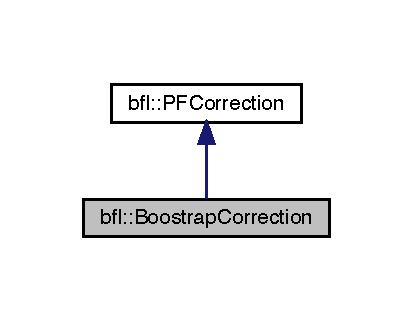
\includegraphics[width=198pt]{classbfl_1_1BoostrapCorrection__inherit__graph}
\end{center}
\end{figure}
\subsection*{Public Member Functions}
\begin{DoxyCompactItemize}
\item 
\mbox{\hyperlink{classbfl_1_1BoostrapCorrection_a0745f5bb495d8afea6cbbbf426ab81ed}{Boostrap\+Correction}} () noexcept
\item 
virtual \mbox{\hyperlink{classbfl_1_1BoostrapCorrection_af99836ae1156168417cac182000cb886}{$\sim$\+Boostrap\+Correction}} () noexcept
\item 
void \mbox{\hyperlink{classbfl_1_1BoostrapCorrection_a75d770c17ac4142833c926e9e6dc32db}{set\+Likelihood\+Model}} (std\+::unique\+\_\+ptr$<$ \mbox{\hyperlink{classbfl_1_1LikelihoodModel}{Likelihood\+Model}} $>$ likelihood\+\_\+model) override
\item 
void \mbox{\hyperlink{classbfl_1_1BoostrapCorrection_af6e02e5d6e6426cbee2825a77c79da43}{set\+Measurement\+Model}} (std\+::unique\+\_\+ptr$<$ \mbox{\hyperlink{classbfl_1_1MeasurementModel}{Measurement\+Model}} $>$ measurement\+\_\+model) override
\item 
std\+::pair$<$ bool, Eigen\+::\+Vector\+Xd $>$ \mbox{\hyperlink{classbfl_1_1BoostrapCorrection_a18ad4ccfd9d7cf008011cbc79a0cea8f}{get\+Likelihood}} () override
\item 
void \mbox{\hyperlink{classbfl_1_1PFCorrection_a560666b2e7566a846cb4ce4684e195e0}{correct}} (const \mbox{\hyperlink{classbfl_1_1ParticleSet}{bfl\+::\+Particle\+Set}} \&pred\+\_\+particles, \mbox{\hyperlink{classbfl_1_1ParticleSet}{bfl\+::\+Particle\+Set}} \&cor\+\_\+particles)
\item 
bool \mbox{\hyperlink{classbfl_1_1PFCorrection_ab25e625ea12fe257e0eb85d465835e62}{skip}} (const bool status)
\end{DoxyCompactItemize}
\subsection*{Protected Member Functions}
\begin{DoxyCompactItemize}
\item 
\mbox{\hyperlink{classbfl_1_1LikelihoodModel}{Likelihood\+Model}} \& \mbox{\hyperlink{classbfl_1_1BoostrapCorrection_aae2f5698ba37895b6193f51441f96f38}{get\+Likelihood\+Model}} () override
\item 
\mbox{\hyperlink{classbfl_1_1MeasurementModel}{Measurement\+Model}} \& \mbox{\hyperlink{classbfl_1_1BoostrapCorrection_a4d11bb3e7e27dcd62bb7e1b5df83c8db}{get\+Measurement\+Model}} () override
\item 
void \mbox{\hyperlink{classbfl_1_1BoostrapCorrection_a493eed345120c5babb0f3591d9c7c854}{correct\+Step}} (const \mbox{\hyperlink{classbfl_1_1ParticleSet}{Particle\+Set}} \&pred\+\_\+particles, \mbox{\hyperlink{classbfl_1_1ParticleSet}{Particle\+Set}} \&cor\+\_\+particles) override
\end{DoxyCompactItemize}
\subsection*{Protected Attributes}
\begin{DoxyCompactItemize}
\item 
std\+::unique\+\_\+ptr$<$ \mbox{\hyperlink{classbfl_1_1LikelihoodModel}{Likelihood\+Model}} $>$ \mbox{\hyperlink{classbfl_1_1BoostrapCorrection_aaef6c382ea35a46474c3c3c7300cf6d9}{likelihood\+\_\+model\+\_\+}}
\item 
std\+::unique\+\_\+ptr$<$ \mbox{\hyperlink{classbfl_1_1MeasurementModel}{Measurement\+Model}} $>$ \mbox{\hyperlink{classbfl_1_1BoostrapCorrection_a06929b7db97b01b7e8e1c0d4f5a19274}{measurement\+\_\+model\+\_\+}}
\item 
bool \mbox{\hyperlink{classbfl_1_1BoostrapCorrection_af61251e64b3d4c0b95af7a2fd6adf0c5}{valid\+\_\+likelihood\+\_\+}} = false
\item 
Eigen\+::\+Vector\+Xd \mbox{\hyperlink{classbfl_1_1BoostrapCorrection_ae35bcabcf28cd7d46f5581c33f1c9390}{likelihood\+\_\+}}
\end{DoxyCompactItemize}


\subsection{Detailed Description}


Definition at line 15 of file Bootstrap\+Correction.\+h.



\subsection{Constructor \& Destructor Documentation}
\mbox{\Hypertarget{classbfl_1_1BoostrapCorrection_a0745f5bb495d8afea6cbbbf426ab81ed}\label{classbfl_1_1BoostrapCorrection_a0745f5bb495d8afea6cbbbf426ab81ed}} 
\index{bfl\+::\+Boostrap\+Correction@{bfl\+::\+Boostrap\+Correction}!Boostrap\+Correction@{Boostrap\+Correction}}
\index{Boostrap\+Correction@{Boostrap\+Correction}!bfl\+::\+Boostrap\+Correction@{bfl\+::\+Boostrap\+Correction}}
\subsubsection{\texorpdfstring{Boostrap\+Correction()}{BoostrapCorrection()}}
{\footnotesize\ttfamily Boostrap\+Correction\+::\+Boostrap\+Correction (\begin{DoxyParamCaption}{ }\end{DoxyParamCaption})\hspace{0.3cm}{\ttfamily [noexcept]}}



Definition at line 10 of file Bootstrap\+Correction.\+cpp.

\mbox{\Hypertarget{classbfl_1_1BoostrapCorrection_af99836ae1156168417cac182000cb886}\label{classbfl_1_1BoostrapCorrection_af99836ae1156168417cac182000cb886}} 
\index{bfl\+::\+Boostrap\+Correction@{bfl\+::\+Boostrap\+Correction}!````~Boostrap\+Correction@{$\sim$\+Boostrap\+Correction}}
\index{````~Boostrap\+Correction@{$\sim$\+Boostrap\+Correction}!bfl\+::\+Boostrap\+Correction@{bfl\+::\+Boostrap\+Correction}}
\subsubsection{\texorpdfstring{$\sim$\+Boostrap\+Correction()}{~BoostrapCorrection()}}
{\footnotesize\ttfamily Boostrap\+Correction\+::$\sim$\+Boostrap\+Correction (\begin{DoxyParamCaption}{ }\end{DoxyParamCaption})\hspace{0.3cm}{\ttfamily [virtual]}, {\ttfamily [noexcept]}}



Definition at line 13 of file Bootstrap\+Correction.\+cpp.



\subsection{Member Function Documentation}
\mbox{\Hypertarget{classbfl_1_1PFCorrection_a560666b2e7566a846cb4ce4684e195e0}\label{classbfl_1_1PFCorrection_a560666b2e7566a846cb4ce4684e195e0}} 
\index{bfl\+::\+Boostrap\+Correction@{bfl\+::\+Boostrap\+Correction}!correct@{correct}}
\index{correct@{correct}!bfl\+::\+Boostrap\+Correction@{bfl\+::\+Boostrap\+Correction}}
\subsubsection{\texorpdfstring{correct()}{correct()}}
{\footnotesize\ttfamily void P\+F\+Correction\+::correct (\begin{DoxyParamCaption}\item[{const \mbox{\hyperlink{classbfl_1_1ParticleSet}{bfl\+::\+Particle\+Set}} \&}]{pred\+\_\+particles,  }\item[{\mbox{\hyperlink{classbfl_1_1ParticleSet}{bfl\+::\+Particle\+Set}} \&}]{cor\+\_\+particles }\end{DoxyParamCaption})\hspace{0.3cm}{\ttfamily [inherited]}}



Definition at line 10 of file P\+F\+Correction.\+cpp.

\mbox{\Hypertarget{classbfl_1_1BoostrapCorrection_a493eed345120c5babb0f3591d9c7c854}\label{classbfl_1_1BoostrapCorrection_a493eed345120c5babb0f3591d9c7c854}} 
\index{bfl\+::\+Boostrap\+Correction@{bfl\+::\+Boostrap\+Correction}!correct\+Step@{correct\+Step}}
\index{correct\+Step@{correct\+Step}!bfl\+::\+Boostrap\+Correction@{bfl\+::\+Boostrap\+Correction}}
\subsubsection{\texorpdfstring{correct\+Step()}{correctStep()}}
{\footnotesize\ttfamily void Boostrap\+Correction\+::correct\+Step (\begin{DoxyParamCaption}\item[{const \mbox{\hyperlink{classbfl_1_1ParticleSet}{Particle\+Set}} \&}]{pred\+\_\+particles,  }\item[{\mbox{\hyperlink{classbfl_1_1ParticleSet}{Particle\+Set}} \&}]{cor\+\_\+particles }\end{DoxyParamCaption})\hspace{0.3cm}{\ttfamily [override]}, {\ttfamily [protected]}, {\ttfamily [virtual]}}



Implements \mbox{\hyperlink{classbfl_1_1PFCorrection_ae0413156a1258d88485e57a983c89af1}{bfl\+::\+P\+F\+Correction}}.



Definition at line 16 of file Bootstrap\+Correction.\+cpp.



References bfl\+::\+Particle\+Set\+::state(), and bfl\+::\+Gaussian\+Mixture\+::weight().

Here is the call graph for this function\+:
\nopagebreak
\begin{figure}[H]
\begin{center}
\leavevmode
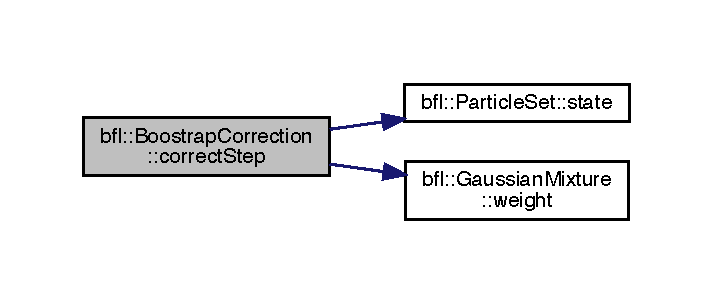
\includegraphics[width=342pt]{classbfl_1_1BoostrapCorrection_a493eed345120c5babb0f3591d9c7c854_cgraph}
\end{center}
\end{figure}
\mbox{\Hypertarget{classbfl_1_1BoostrapCorrection_a18ad4ccfd9d7cf008011cbc79a0cea8f}\label{classbfl_1_1BoostrapCorrection_a18ad4ccfd9d7cf008011cbc79a0cea8f}} 
\index{bfl\+::\+Boostrap\+Correction@{bfl\+::\+Boostrap\+Correction}!get\+Likelihood@{get\+Likelihood}}
\index{get\+Likelihood@{get\+Likelihood}!bfl\+::\+Boostrap\+Correction@{bfl\+::\+Boostrap\+Correction}}
\subsubsection{\texorpdfstring{get\+Likelihood()}{getLikelihood()}}
{\footnotesize\ttfamily std\+::pair$<$ bool, Vector\+Xd $>$ Boostrap\+Correction\+::get\+Likelihood (\begin{DoxyParamCaption}{ }\end{DoxyParamCaption})\hspace{0.3cm}{\ttfamily [override]}, {\ttfamily [virtual]}}



Implements \mbox{\hyperlink{classbfl_1_1PFCorrection_ab6eca766077c4ab1db3417dab6c44d27}{bfl\+::\+P\+F\+Correction}}.



Definition at line 27 of file Bootstrap\+Correction.\+cpp.

\mbox{\Hypertarget{classbfl_1_1BoostrapCorrection_aae2f5698ba37895b6193f51441f96f38}\label{classbfl_1_1BoostrapCorrection_aae2f5698ba37895b6193f51441f96f38}} 
\index{bfl\+::\+Boostrap\+Correction@{bfl\+::\+Boostrap\+Correction}!get\+Likelihood\+Model@{get\+Likelihood\+Model}}
\index{get\+Likelihood\+Model@{get\+Likelihood\+Model}!bfl\+::\+Boostrap\+Correction@{bfl\+::\+Boostrap\+Correction}}
\subsubsection{\texorpdfstring{get\+Likelihood\+Model()}{getLikelihoodModel()}}
{\footnotesize\ttfamily \mbox{\hyperlink{classbfl_1_1LikelihoodModel}{Likelihood\+Model}} \& Boostrap\+Correction\+::get\+Likelihood\+Model (\begin{DoxyParamCaption}{ }\end{DoxyParamCaption})\hspace{0.3cm}{\ttfamily [override]}, {\ttfamily [protected]}, {\ttfamily [virtual]}}



Implements \mbox{\hyperlink{classbfl_1_1PFCorrection_ad812d0b488e0882b246dd19d4f6818e1}{bfl\+::\+P\+F\+Correction}}.



Definition at line 45 of file Bootstrap\+Correction.\+cpp.

\mbox{\Hypertarget{classbfl_1_1BoostrapCorrection_a4d11bb3e7e27dcd62bb7e1b5df83c8db}\label{classbfl_1_1BoostrapCorrection_a4d11bb3e7e27dcd62bb7e1b5df83c8db}} 
\index{bfl\+::\+Boostrap\+Correction@{bfl\+::\+Boostrap\+Correction}!get\+Measurement\+Model@{get\+Measurement\+Model}}
\index{get\+Measurement\+Model@{get\+Measurement\+Model}!bfl\+::\+Boostrap\+Correction@{bfl\+::\+Boostrap\+Correction}}
\subsubsection{\texorpdfstring{get\+Measurement\+Model()}{getMeasurementModel()}}
{\footnotesize\ttfamily \mbox{\hyperlink{classbfl_1_1MeasurementModel}{Measurement\+Model}} \& Boostrap\+Correction\+::get\+Measurement\+Model (\begin{DoxyParamCaption}{ }\end{DoxyParamCaption})\hspace{0.3cm}{\ttfamily [override]}, {\ttfamily [protected]}, {\ttfamily [virtual]}}



Implements \mbox{\hyperlink{classbfl_1_1PFCorrection_a891c7d498caffb4d11e5ebdaa475c683}{bfl\+::\+P\+F\+Correction}}.



Definition at line 51 of file Bootstrap\+Correction.\+cpp.

\mbox{\Hypertarget{classbfl_1_1BoostrapCorrection_a75d770c17ac4142833c926e9e6dc32db}\label{classbfl_1_1BoostrapCorrection_a75d770c17ac4142833c926e9e6dc32db}} 
\index{bfl\+::\+Boostrap\+Correction@{bfl\+::\+Boostrap\+Correction}!set\+Likelihood\+Model@{set\+Likelihood\+Model}}
\index{set\+Likelihood\+Model@{set\+Likelihood\+Model}!bfl\+::\+Boostrap\+Correction@{bfl\+::\+Boostrap\+Correction}}
\subsubsection{\texorpdfstring{set\+Likelihood\+Model()}{setLikelihoodModel()}}
{\footnotesize\ttfamily void Boostrap\+Correction\+::set\+Likelihood\+Model (\begin{DoxyParamCaption}\item[{std\+::unique\+\_\+ptr$<$ \mbox{\hyperlink{classbfl_1_1LikelihoodModel}{Likelihood\+Model}} $>$}]{likelihood\+\_\+model }\end{DoxyParamCaption})\hspace{0.3cm}{\ttfamily [override]}, {\ttfamily [virtual]}}



Implements \mbox{\hyperlink{classbfl_1_1PFCorrection_aa84e757c694d4ad375cdd543d42ac34c}{bfl\+::\+P\+F\+Correction}}.



Definition at line 33 of file Bootstrap\+Correction.\+cpp.

\mbox{\Hypertarget{classbfl_1_1BoostrapCorrection_af6e02e5d6e6426cbee2825a77c79da43}\label{classbfl_1_1BoostrapCorrection_af6e02e5d6e6426cbee2825a77c79da43}} 
\index{bfl\+::\+Boostrap\+Correction@{bfl\+::\+Boostrap\+Correction}!set\+Measurement\+Model@{set\+Measurement\+Model}}
\index{set\+Measurement\+Model@{set\+Measurement\+Model}!bfl\+::\+Boostrap\+Correction@{bfl\+::\+Boostrap\+Correction}}
\subsubsection{\texorpdfstring{set\+Measurement\+Model()}{setMeasurementModel()}}
{\footnotesize\ttfamily void Boostrap\+Correction\+::set\+Measurement\+Model (\begin{DoxyParamCaption}\item[{std\+::unique\+\_\+ptr$<$ \mbox{\hyperlink{classbfl_1_1MeasurementModel}{Measurement\+Model}} $>$}]{measurement\+\_\+model }\end{DoxyParamCaption})\hspace{0.3cm}{\ttfamily [override]}, {\ttfamily [virtual]}}



Implements \mbox{\hyperlink{classbfl_1_1PFCorrection_a9844514568f65a0e5fa2cffadea460c6}{bfl\+::\+P\+F\+Correction}}.



Definition at line 39 of file Bootstrap\+Correction.\+cpp.

\mbox{\Hypertarget{classbfl_1_1PFCorrection_ab25e625ea12fe257e0eb85d465835e62}\label{classbfl_1_1PFCorrection_ab25e625ea12fe257e0eb85d465835e62}} 
\index{bfl\+::\+Boostrap\+Correction@{bfl\+::\+Boostrap\+Correction}!skip@{skip}}
\index{skip@{skip}!bfl\+::\+Boostrap\+Correction@{bfl\+::\+Boostrap\+Correction}}
\subsubsection{\texorpdfstring{skip()}{skip()}}
{\footnotesize\ttfamily bool P\+F\+Correction\+::skip (\begin{DoxyParamCaption}\item[{const bool}]{status }\end{DoxyParamCaption})\hspace{0.3cm}{\ttfamily [inherited]}}



Definition at line 20 of file P\+F\+Correction.\+cpp.



\subsection{Member Data Documentation}
\mbox{\Hypertarget{classbfl_1_1BoostrapCorrection_ae35bcabcf28cd7d46f5581c33f1c9390}\label{classbfl_1_1BoostrapCorrection_ae35bcabcf28cd7d46f5581c33f1c9390}} 
\index{bfl\+::\+Boostrap\+Correction@{bfl\+::\+Boostrap\+Correction}!likelihood\+\_\+@{likelihood\+\_\+}}
\index{likelihood\+\_\+@{likelihood\+\_\+}!bfl\+::\+Boostrap\+Correction@{bfl\+::\+Boostrap\+Correction}}
\subsubsection{\texorpdfstring{likelihood\+\_\+}{likelihood\_}}
{\footnotesize\ttfamily Eigen\+::\+Vector\+Xd bfl\+::\+Boostrap\+Correction\+::likelihood\+\_\+\hspace{0.3cm}{\ttfamily [protected]}}



Definition at line 40 of file Bootstrap\+Correction.\+h.

\mbox{\Hypertarget{classbfl_1_1BoostrapCorrection_aaef6c382ea35a46474c3c3c7300cf6d9}\label{classbfl_1_1BoostrapCorrection_aaef6c382ea35a46474c3c3c7300cf6d9}} 
\index{bfl\+::\+Boostrap\+Correction@{bfl\+::\+Boostrap\+Correction}!likelihood\+\_\+model\+\_\+@{likelihood\+\_\+model\+\_\+}}
\index{likelihood\+\_\+model\+\_\+@{likelihood\+\_\+model\+\_\+}!bfl\+::\+Boostrap\+Correction@{bfl\+::\+Boostrap\+Correction}}
\subsubsection{\texorpdfstring{likelihood\+\_\+model\+\_\+}{likelihood\_model\_}}
{\footnotesize\ttfamily std\+::unique\+\_\+ptr$<$\mbox{\hyperlink{classbfl_1_1LikelihoodModel}{Likelihood\+Model}}$>$ bfl\+::\+Boostrap\+Correction\+::likelihood\+\_\+model\+\_\+\hspace{0.3cm}{\ttfamily [protected]}}



Definition at line 29 of file Bootstrap\+Correction.\+h.

\mbox{\Hypertarget{classbfl_1_1BoostrapCorrection_a06929b7db97b01b7e8e1c0d4f5a19274}\label{classbfl_1_1BoostrapCorrection_a06929b7db97b01b7e8e1c0d4f5a19274}} 
\index{bfl\+::\+Boostrap\+Correction@{bfl\+::\+Boostrap\+Correction}!measurement\+\_\+model\+\_\+@{measurement\+\_\+model\+\_\+}}
\index{measurement\+\_\+model\+\_\+@{measurement\+\_\+model\+\_\+}!bfl\+::\+Boostrap\+Correction@{bfl\+::\+Boostrap\+Correction}}
\subsubsection{\texorpdfstring{measurement\+\_\+model\+\_\+}{measurement\_model\_}}
{\footnotesize\ttfamily std\+::unique\+\_\+ptr$<$\mbox{\hyperlink{classbfl_1_1MeasurementModel}{Measurement\+Model}}$>$ bfl\+::\+Boostrap\+Correction\+::measurement\+\_\+model\+\_\+\hspace{0.3cm}{\ttfamily [protected]}}



Definition at line 31 of file Bootstrap\+Correction.\+h.

\mbox{\Hypertarget{classbfl_1_1BoostrapCorrection_af61251e64b3d4c0b95af7a2fd6adf0c5}\label{classbfl_1_1BoostrapCorrection_af61251e64b3d4c0b95af7a2fd6adf0c5}} 
\index{bfl\+::\+Boostrap\+Correction@{bfl\+::\+Boostrap\+Correction}!valid\+\_\+likelihood\+\_\+@{valid\+\_\+likelihood\+\_\+}}
\index{valid\+\_\+likelihood\+\_\+@{valid\+\_\+likelihood\+\_\+}!bfl\+::\+Boostrap\+Correction@{bfl\+::\+Boostrap\+Correction}}
\subsubsection{\texorpdfstring{valid\+\_\+likelihood\+\_\+}{valid\_likelihood\_}}
{\footnotesize\ttfamily bool bfl\+::\+Boostrap\+Correction\+::valid\+\_\+likelihood\+\_\+ = false\hspace{0.3cm}{\ttfamily [protected]}}



Definition at line 39 of file Bootstrap\+Correction.\+h.



The documentation for this class was generated from the following files\+:\begin{DoxyCompactItemize}
\item 
/\+Users/\+Claudio/\+Git\+Hub/bayes-\/filters-\/lib/src/\+Bayes\+Filters/include/\+Bayes\+Filters/\mbox{\hyperlink{BootstrapCorrection_8h}{Bootstrap\+Correction.\+h}}\item 
/\+Users/\+Claudio/\+Git\+Hub/bayes-\/filters-\/lib/src/\+Bayes\+Filters/src/\mbox{\hyperlink{BootstrapCorrection_8cpp}{Bootstrap\+Correction.\+cpp}}\end{DoxyCompactItemize}

\hypertarget{classbfl_1_1DrawParticles}{}\section{bfl\+:\+:Draw\+Particles Class Reference}
\label{classbfl_1_1DrawParticles}\index{bfl\+::\+Draw\+Particles@{bfl\+::\+Draw\+Particles}}


{\ttfamily \#include $<$Draw\+Particles.\+h$>$}



Inheritance diagram for bfl\+:\+:Draw\+Particles\+:
\nopagebreak
\begin{figure}[H]
\begin{center}
\leavevmode
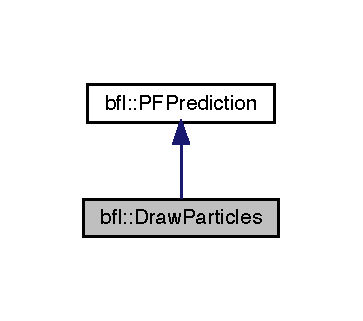
\includegraphics[width=174pt]{classbfl_1_1DrawParticles__inherit__graph}
\end{center}
\end{figure}
\subsection*{Public Member Functions}
\begin{DoxyCompactItemize}
\item 
\mbox{\hyperlink{classbfl_1_1DrawParticles_acd7269927dc19bf3f34f7a65934c1e2c}{Draw\+Particles}} () noexcept
\item 
\mbox{\hyperlink{classbfl_1_1DrawParticles_aa5ef8dc20a4c5fac0f30531fbe5a1ecd}{Draw\+Particles}} (\mbox{\hyperlink{classbfl_1_1DrawParticles}{Draw\+Particles}} \&\&draw\+\_\+particles) noexcept
\item 
virtual \mbox{\hyperlink{classbfl_1_1DrawParticles_a7acfdc073d85f1425c2d8d9ba1339896}{$\sim$\+Draw\+Particles}} () noexcept
\item 
virtual \mbox{\hyperlink{classbfl_1_1StateModel}{State\+Model}} \& \mbox{\hyperlink{classbfl_1_1DrawParticles_a7a7ebf5a7ea10747db1bd8ab03390107}{get\+State\+Model}} () override
\item 
virtual void \mbox{\hyperlink{classbfl_1_1DrawParticles_acb607ab90c22a43a72a75576acb898a4}{set\+State\+Model}} (std\+::unique\+\_\+ptr$<$ \mbox{\hyperlink{classbfl_1_1StateModel}{State\+Model}} $>$ state\+\_\+model) override
\item 
void \mbox{\hyperlink{classbfl_1_1PFPrediction_a129dcd1cccd2da9827ef0c49c90b9345}{predict}} (const \mbox{\hyperlink{classbfl_1_1ParticleSet}{bfl\+::\+Particle\+Set}} \&prev\+\_\+particles, \mbox{\hyperlink{classbfl_1_1ParticleSet}{bfl\+::\+Particle\+Set}} \&pred\+\_\+particles)
\item 
bool \mbox{\hyperlink{classbfl_1_1PFPrediction_a364cc35a151e5298c4024d681f3e04d9}{skip}} (const std\+::string \&what\+\_\+step, const bool status)
\item 
bool \mbox{\hyperlink{classbfl_1_1PFPrediction_a323ca5612dd7ad924fd448a629359ad2}{get\+Skip\+State}} ()
\item 
bool \mbox{\hyperlink{classbfl_1_1PFPrediction_a432b8e84dbf00432158aa82312386d63}{get\+Skip\+Exogenous}} ()
\item 
virtual void \mbox{\hyperlink{classbfl_1_1PFPrediction_ada843698204584e97d4ff6728c8e8264}{set\+Exogenous\+Model}} (std\+::unique\+\_\+ptr$<$ \mbox{\hyperlink{classbfl_1_1ExogenousModel}{Exogenous\+Model}} $>$ exogenous\+\_\+model)
\item 
virtual \mbox{\hyperlink{classbfl_1_1ExogenousModel}{Exogenous\+Model}} \& \mbox{\hyperlink{classbfl_1_1PFPrediction_aefa127a440649447e8ac659ef65b7a2a}{get\+Exogenous\+Model}} ()
\end{DoxyCompactItemize}
\subsection*{Protected Member Functions}
\begin{DoxyCompactItemize}
\item 
void \mbox{\hyperlink{classbfl_1_1DrawParticles_a36deaed86f1146431cacefa23f0445d0}{predict\+Step}} (const \mbox{\hyperlink{classbfl_1_1ParticleSet}{Particle\+Set}} \&prev\+\_\+particles, \mbox{\hyperlink{classbfl_1_1ParticleSet}{Particle\+Set}} \&pred\+\_\+particles) override
\end{DoxyCompactItemize}
\subsection*{Protected Attributes}
\begin{DoxyCompactItemize}
\item 
std\+::unique\+\_\+ptr$<$ \mbox{\hyperlink{classbfl_1_1StateModel}{State\+Model}} $>$ \mbox{\hyperlink{classbfl_1_1DrawParticles_a4acbc6e750895a3a27e68d0a9656b8cf}{state\+\_\+model\+\_\+}}
\end{DoxyCompactItemize}


\subsection{Detailed Description}


Definition at line 15 of file Draw\+Particles.\+h.



\subsection{Constructor \& Destructor Documentation}
\mbox{\Hypertarget{classbfl_1_1DrawParticles_acd7269927dc19bf3f34f7a65934c1e2c}\label{classbfl_1_1DrawParticles_acd7269927dc19bf3f34f7a65934c1e2c}} 
\index{bfl\+::\+Draw\+Particles@{bfl\+::\+Draw\+Particles}!Draw\+Particles@{Draw\+Particles}}
\index{Draw\+Particles@{Draw\+Particles}!bfl\+::\+Draw\+Particles@{bfl\+::\+Draw\+Particles}}
\subsubsection{\texorpdfstring{Draw\+Particles()}{DrawParticles()}\hspace{0.1cm}{\footnotesize\ttfamily [1/2]}}
{\footnotesize\ttfamily Draw\+Particles\+::\+Draw\+Particles (\begin{DoxyParamCaption}{ }\end{DoxyParamCaption})\hspace{0.3cm}{\ttfamily [noexcept]}}



Definition at line 9 of file Draw\+Particles.\+cpp.

\mbox{\Hypertarget{classbfl_1_1DrawParticles_aa5ef8dc20a4c5fac0f30531fbe5a1ecd}\label{classbfl_1_1DrawParticles_aa5ef8dc20a4c5fac0f30531fbe5a1ecd}} 
\index{bfl\+::\+Draw\+Particles@{bfl\+::\+Draw\+Particles}!Draw\+Particles@{Draw\+Particles}}
\index{Draw\+Particles@{Draw\+Particles}!bfl\+::\+Draw\+Particles@{bfl\+::\+Draw\+Particles}}
\subsubsection{\texorpdfstring{Draw\+Particles()}{DrawParticles()}\hspace{0.1cm}{\footnotesize\ttfamily [2/2]}}
{\footnotesize\ttfamily Draw\+Particles\+::\+Draw\+Particles (\begin{DoxyParamCaption}\item[{\mbox{\hyperlink{classbfl_1_1DrawParticles}{Draw\+Particles}} \&\&}]{draw\+\_\+particles }\end{DoxyParamCaption})\hspace{0.3cm}{\ttfamily [noexcept]}}



Definition at line 12 of file Draw\+Particles.\+cpp.

\mbox{\Hypertarget{classbfl_1_1DrawParticles_a7acfdc073d85f1425c2d8d9ba1339896}\label{classbfl_1_1DrawParticles_a7acfdc073d85f1425c2d8d9ba1339896}} 
\index{bfl\+::\+Draw\+Particles@{bfl\+::\+Draw\+Particles}!````~Draw\+Particles@{$\sim$\+Draw\+Particles}}
\index{````~Draw\+Particles@{$\sim$\+Draw\+Particles}!bfl\+::\+Draw\+Particles@{bfl\+::\+Draw\+Particles}}
\subsubsection{\texorpdfstring{$\sim$\+Draw\+Particles()}{~DrawParticles()}}
{\footnotesize\ttfamily Draw\+Particles\+::$\sim$\+Draw\+Particles (\begin{DoxyParamCaption}{ }\end{DoxyParamCaption})\hspace{0.3cm}{\ttfamily [virtual]}, {\ttfamily [noexcept]}}



Definition at line 16 of file Draw\+Particles.\+cpp.



\subsection{Member Function Documentation}
\mbox{\Hypertarget{classbfl_1_1PFPrediction_aefa127a440649447e8ac659ef65b7a2a}\label{classbfl_1_1PFPrediction_aefa127a440649447e8ac659ef65b7a2a}} 
\index{bfl\+::\+Draw\+Particles@{bfl\+::\+Draw\+Particles}!get\+Exogenous\+Model@{get\+Exogenous\+Model}}
\index{get\+Exogenous\+Model@{get\+Exogenous\+Model}!bfl\+::\+Draw\+Particles@{bfl\+::\+Draw\+Particles}}
\subsubsection{\texorpdfstring{get\+Exogenous\+Model()}{getExogenousModel()}}
{\footnotesize\ttfamily \mbox{\hyperlink{classbfl_1_1ExogenousModel}{Exogenous\+Model}} \& P\+F\+Prediction\+::get\+Exogenous\+Model (\begin{DoxyParamCaption}{ }\end{DoxyParamCaption})\hspace{0.3cm}{\ttfamily [virtual]}, {\ttfamily [inherited]}}



Reimplemented in \mbox{\hyperlink{classbfl_1_1PFPredictionDecorator_a8d25d3765f642f7de1af897d088d8da9}{bfl\+::\+P\+F\+Prediction\+Decorator}}.



Definition at line 60 of file P\+F\+Prediction.\+cpp.

\mbox{\Hypertarget{classbfl_1_1PFPrediction_a432b8e84dbf00432158aa82312386d63}\label{classbfl_1_1PFPrediction_a432b8e84dbf00432158aa82312386d63}} 
\index{bfl\+::\+Draw\+Particles@{bfl\+::\+Draw\+Particles}!get\+Skip\+Exogenous@{get\+Skip\+Exogenous}}
\index{get\+Skip\+Exogenous@{get\+Skip\+Exogenous}!bfl\+::\+Draw\+Particles@{bfl\+::\+Draw\+Particles}}
\subsubsection{\texorpdfstring{get\+Skip\+Exogenous()}{getSkipExogenous()}}
{\footnotesize\ttfamily bool P\+F\+Prediction\+::get\+Skip\+Exogenous (\begin{DoxyParamCaption}{ }\end{DoxyParamCaption})\hspace{0.3cm}{\ttfamily [inherited]}}



Definition at line 54 of file P\+F\+Prediction.\+cpp.

\mbox{\Hypertarget{classbfl_1_1PFPrediction_a323ca5612dd7ad924fd448a629359ad2}\label{classbfl_1_1PFPrediction_a323ca5612dd7ad924fd448a629359ad2}} 
\index{bfl\+::\+Draw\+Particles@{bfl\+::\+Draw\+Particles}!get\+Skip\+State@{get\+Skip\+State}}
\index{get\+Skip\+State@{get\+Skip\+State}!bfl\+::\+Draw\+Particles@{bfl\+::\+Draw\+Particles}}
\subsubsection{\texorpdfstring{get\+Skip\+State()}{getSkipState()}}
{\footnotesize\ttfamily bool P\+F\+Prediction\+::get\+Skip\+State (\begin{DoxyParamCaption}{ }\end{DoxyParamCaption})\hspace{0.3cm}{\ttfamily [inherited]}}



Definition at line 48 of file P\+F\+Prediction.\+cpp.

\mbox{\Hypertarget{classbfl_1_1DrawParticles_a7a7ebf5a7ea10747db1bd8ab03390107}\label{classbfl_1_1DrawParticles_a7a7ebf5a7ea10747db1bd8ab03390107}} 
\index{bfl\+::\+Draw\+Particles@{bfl\+::\+Draw\+Particles}!get\+State\+Model@{get\+State\+Model}}
\index{get\+State\+Model@{get\+State\+Model}!bfl\+::\+Draw\+Particles@{bfl\+::\+Draw\+Particles}}
\subsubsection{\texorpdfstring{get\+State\+Model()}{getStateModel()}}
{\footnotesize\ttfamily \mbox{\hyperlink{classbfl_1_1StateModel}{State\+Model}} \& Draw\+Particles\+::get\+State\+Model (\begin{DoxyParamCaption}{ }\end{DoxyParamCaption})\hspace{0.3cm}{\ttfamily [override]}, {\ttfamily [virtual]}}



Implements \mbox{\hyperlink{classbfl_1_1PFPrediction_a1a0f7a1d66a6849c2de10459c6b8f8ac}{bfl\+::\+P\+F\+Prediction}}.



Definition at line 26 of file Draw\+Particles.\+cpp.

\mbox{\Hypertarget{classbfl_1_1PFPrediction_a129dcd1cccd2da9827ef0c49c90b9345}\label{classbfl_1_1PFPrediction_a129dcd1cccd2da9827ef0c49c90b9345}} 
\index{bfl\+::\+Draw\+Particles@{bfl\+::\+Draw\+Particles}!predict@{predict}}
\index{predict@{predict}!bfl\+::\+Draw\+Particles@{bfl\+::\+Draw\+Particles}}
\subsubsection{\texorpdfstring{predict()}{predict()}}
{\footnotesize\ttfamily void P\+F\+Prediction\+::predict (\begin{DoxyParamCaption}\item[{const \mbox{\hyperlink{classbfl_1_1ParticleSet}{bfl\+::\+Particle\+Set}} \&}]{prev\+\_\+particles,  }\item[{\mbox{\hyperlink{classbfl_1_1ParticleSet}{bfl\+::\+Particle\+Set}} \&}]{pred\+\_\+particles }\end{DoxyParamCaption})\hspace{0.3cm}{\ttfamily [inherited]}}



Definition at line 24 of file P\+F\+Prediction.\+cpp.

\mbox{\Hypertarget{classbfl_1_1DrawParticles_a36deaed86f1146431cacefa23f0445d0}\label{classbfl_1_1DrawParticles_a36deaed86f1146431cacefa23f0445d0}} 
\index{bfl\+::\+Draw\+Particles@{bfl\+::\+Draw\+Particles}!predict\+Step@{predict\+Step}}
\index{predict\+Step@{predict\+Step}!bfl\+::\+Draw\+Particles@{bfl\+::\+Draw\+Particles}}
\subsubsection{\texorpdfstring{predict\+Step()}{predictStep()}}
{\footnotesize\ttfamily void Draw\+Particles\+::predict\+Step (\begin{DoxyParamCaption}\item[{const \mbox{\hyperlink{classbfl_1_1ParticleSet}{Particle\+Set}} \&}]{prev\+\_\+particles,  }\item[{\mbox{\hyperlink{classbfl_1_1ParticleSet}{Particle\+Set}} \&}]{pred\+\_\+particles }\end{DoxyParamCaption})\hspace{0.3cm}{\ttfamily [override]}, {\ttfamily [protected]}, {\ttfamily [virtual]}}



Implements \mbox{\hyperlink{classbfl_1_1PFPrediction_ade49953e2beed6d12f9716254ccbba71}{bfl\+::\+P\+F\+Prediction}}.



Definition at line 19 of file Draw\+Particles.\+cpp.



References bfl\+::\+Particle\+Set\+::state(), and bfl\+::\+Gaussian\+Mixture\+::weight().

Here is the call graph for this function\+:
\nopagebreak
\begin{figure}[H]
\begin{center}
\leavevmode
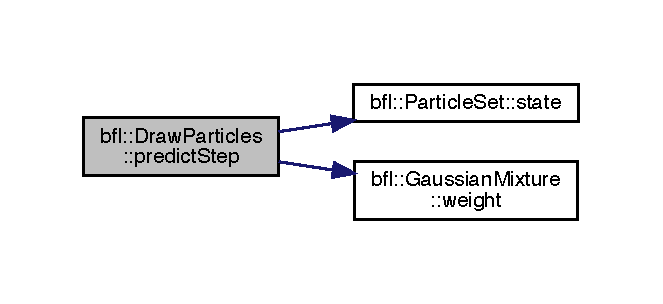
\includegraphics[width=318pt]{classbfl_1_1DrawParticles_a36deaed86f1146431cacefa23f0445d0_cgraph}
\end{center}
\end{figure}
\mbox{\Hypertarget{classbfl_1_1PFPrediction_ada843698204584e97d4ff6728c8e8264}\label{classbfl_1_1PFPrediction_ada843698204584e97d4ff6728c8e8264}} 
\index{bfl\+::\+Draw\+Particles@{bfl\+::\+Draw\+Particles}!set\+Exogenous\+Model@{set\+Exogenous\+Model}}
\index{set\+Exogenous\+Model@{set\+Exogenous\+Model}!bfl\+::\+Draw\+Particles@{bfl\+::\+Draw\+Particles}}
\subsubsection{\texorpdfstring{set\+Exogenous\+Model()}{setExogenousModel()}}
{\footnotesize\ttfamily void P\+F\+Prediction\+::set\+Exogenous\+Model (\begin{DoxyParamCaption}\item[{std\+::unique\+\_\+ptr$<$ \mbox{\hyperlink{classbfl_1_1ExogenousModel}{Exogenous\+Model}} $>$}]{exogenous\+\_\+model }\end{DoxyParamCaption})\hspace{0.3cm}{\ttfamily [virtual]}, {\ttfamily [inherited]}}



Reimplemented in \mbox{\hyperlink{classbfl_1_1PFPredictionDecorator_a3c38ae386456ecd0fd1b609b381395ec}{bfl\+::\+P\+F\+Prediction\+Decorator}}.



Definition at line 66 of file P\+F\+Prediction.\+cpp.

\mbox{\Hypertarget{classbfl_1_1DrawParticles_acb607ab90c22a43a72a75576acb898a4}\label{classbfl_1_1DrawParticles_acb607ab90c22a43a72a75576acb898a4}} 
\index{bfl\+::\+Draw\+Particles@{bfl\+::\+Draw\+Particles}!set\+State\+Model@{set\+State\+Model}}
\index{set\+State\+Model@{set\+State\+Model}!bfl\+::\+Draw\+Particles@{bfl\+::\+Draw\+Particles}}
\subsubsection{\texorpdfstring{set\+State\+Model()}{setStateModel()}}
{\footnotesize\ttfamily void Draw\+Particles\+::set\+State\+Model (\begin{DoxyParamCaption}\item[{std\+::unique\+\_\+ptr$<$ \mbox{\hyperlink{classbfl_1_1StateModel}{State\+Model}} $>$}]{state\+\_\+model }\end{DoxyParamCaption})\hspace{0.3cm}{\ttfamily [override]}, {\ttfamily [virtual]}}



Implements \mbox{\hyperlink{classbfl_1_1PFPrediction_ac39683650d7f89c59f1426dd7743354e}{bfl\+::\+P\+F\+Prediction}}.



Definition at line 32 of file Draw\+Particles.\+cpp.

\mbox{\Hypertarget{classbfl_1_1PFPrediction_a364cc35a151e5298c4024d681f3e04d9}\label{classbfl_1_1PFPrediction_a364cc35a151e5298c4024d681f3e04d9}} 
\index{bfl\+::\+Draw\+Particles@{bfl\+::\+Draw\+Particles}!skip@{skip}}
\index{skip@{skip}!bfl\+::\+Draw\+Particles@{bfl\+::\+Draw\+Particles}}
\subsubsection{\texorpdfstring{skip()}{skip()}}
{\footnotesize\ttfamily bool P\+F\+Prediction\+::skip (\begin{DoxyParamCaption}\item[{const std\+::string \&}]{what\+\_\+step,  }\item[{const bool}]{status }\end{DoxyParamCaption})\hspace{0.3cm}{\ttfamily [inherited]}}



Definition at line 33 of file P\+F\+Prediction.\+cpp.



\subsection{Member Data Documentation}
\mbox{\Hypertarget{classbfl_1_1DrawParticles_a4acbc6e750895a3a27e68d0a9656b8cf}\label{classbfl_1_1DrawParticles_a4acbc6e750895a3a27e68d0a9656b8cf}} 
\index{bfl\+::\+Draw\+Particles@{bfl\+::\+Draw\+Particles}!state\+\_\+model\+\_\+@{state\+\_\+model\+\_\+}}
\index{state\+\_\+model\+\_\+@{state\+\_\+model\+\_\+}!bfl\+::\+Draw\+Particles@{bfl\+::\+Draw\+Particles}}
\subsubsection{\texorpdfstring{state\+\_\+model\+\_\+}{state\_model\_}}
{\footnotesize\ttfamily std\+::unique\+\_\+ptr$<$\mbox{\hyperlink{classbfl_1_1StateModel}{State\+Model}}$>$ bfl\+::\+Draw\+Particles\+::state\+\_\+model\+\_\+\hspace{0.3cm}{\ttfamily [protected]}}



Definition at line 31 of file Draw\+Particles.\+h.



The documentation for this class was generated from the following files\+:\begin{DoxyCompactItemize}
\item 
/\+Users/\+Claudio/\+Git\+Hub/bayes-\/filters-\/lib/src/\+Bayes\+Filters/include/\+Bayes\+Filters/\mbox{\hyperlink{DrawParticles_8h}{Draw\+Particles.\+h}}\item 
/\+Users/\+Claudio/\+Git\+Hub/bayes-\/filters-\/lib/src/\+Bayes\+Filters/src/\mbox{\hyperlink{DrawParticles_8cpp}{Draw\+Particles.\+cpp}}\end{DoxyCompactItemize}

\hypertarget{classbfl_1_1EstimatesExtraction}{}\section{bfl\+:\+:Estimates\+Extraction Class Reference}
\label{classbfl_1_1EstimatesExtraction}\index{bfl\+::\+Estimates\+Extraction@{bfl\+::\+Estimates\+Extraction}}


{\ttfamily \#include $<$Estimates\+Extraction.\+h$>$}

\subsection*{Public Types}
\begin{DoxyCompactItemize}
\item 
enum \mbox{\hyperlink{classbfl_1_1EstimatesExtraction_a8489976af4025f0bbc3288ff7f17ffb0}{Extraction\+Method}} \{ \newline
\mbox{\hyperlink{classbfl_1_1EstimatesExtraction_a8489976af4025f0bbc3288ff7f17ffb0ab93db188572fc4d76cce5660f3823b0a}{Extraction\+Method\+::mean}}, 
\mbox{\hyperlink{classbfl_1_1EstimatesExtraction_a8489976af4025f0bbc3288ff7f17ffb0abbc9c90f98a268f78971d2e670dd527e}{Extraction\+Method\+::smean}}, 
\mbox{\hyperlink{classbfl_1_1EstimatesExtraction_a8489976af4025f0bbc3288ff7f17ffb0a1d2c4e9e69cf765aa9ff84e8a69501cd}{Extraction\+Method\+::wmean}}, 
\mbox{\hyperlink{classbfl_1_1EstimatesExtraction_a8489976af4025f0bbc3288ff7f17ffb0a1f31c7680951dbcb0768323cfd1e7726}{Extraction\+Method\+::emean}}, 
\newline
\mbox{\hyperlink{classbfl_1_1EstimatesExtraction_a8489976af4025f0bbc3288ff7f17ffb0a15d61712450a686a7f365adf4fef581f}{Extraction\+Method\+::mode}}, 
\mbox{\hyperlink{classbfl_1_1EstimatesExtraction_a8489976af4025f0bbc3288ff7f17ffb0a2c3917a1bbad7f91dfa6d1d524e83888}{Extraction\+Method\+::smode}}, 
\mbox{\hyperlink{classbfl_1_1EstimatesExtraction_a8489976af4025f0bbc3288ff7f17ffb0ac6e4db54fbd05bde785ef07a442b50f5}{Extraction\+Method\+::wmode}}, 
\mbox{\hyperlink{classbfl_1_1EstimatesExtraction_a8489976af4025f0bbc3288ff7f17ffb0a68aa9a30f26a7648656847fd30c44144}{Extraction\+Method\+::emode}}
 \}
\end{DoxyCompactItemize}
\subsection*{Public Member Functions}
\begin{DoxyCompactItemize}
\item 
\mbox{\hyperlink{classbfl_1_1EstimatesExtraction_a49ab15a22c1766a16cd6ccc29447dd49}{Estimates\+Extraction}} () noexcept
\item 
\mbox{\hyperlink{classbfl_1_1EstimatesExtraction_a3d16bdd9dbc8841eae07cfdc3aa52114}{Estimates\+Extraction}} (\mbox{\hyperlink{classbfl_1_1EstimatesExtraction}{Estimates\+Extraction}} \&\&estimate\+\_\+extraction) noexcept
\item 
\mbox{\hyperlink{classbfl_1_1EstimatesExtraction}{Estimates\+Extraction}} \& \mbox{\hyperlink{classbfl_1_1EstimatesExtraction_ae473904953c7ad90408da2b4d3c14a1a}{operator=}} (\mbox{\hyperlink{classbfl_1_1EstimatesExtraction}{Estimates\+Extraction}} \&\&estimate\+\_\+extraction) noexcept
\item 
\mbox{\hyperlink{classbfl_1_1EstimatesExtraction_af7a89d920cc8e4ebbef66c1dfce37ecb}{$\sim$\+Estimates\+Extraction}} () noexcept
\item 
bool \mbox{\hyperlink{classbfl_1_1EstimatesExtraction_a68bb4f3b41f578a38d9847b9c140c130}{set\+Method}} (const \mbox{\hyperlink{classbfl_1_1EstimatesExtraction_a8489976af4025f0bbc3288ff7f17ffb0}{Extraction\+Method}} \&extraction\+\_\+method)
\item 
bool \mbox{\hyperlink{classbfl_1_1EstimatesExtraction_a49babb0803c50d697b8d21014010f5bb}{set\+Mobile\+Average\+Window\+Size}} (const int window)
\item 
Eigen\+::\+Vector\+Xd \mbox{\hyperlink{classbfl_1_1EstimatesExtraction_aeb792e7d2e162c13f66903551ff82dfa}{extract}} (const Eigen\+::\+Ref$<$ const Eigen\+::\+Matrix\+Xd $>$ \&particles, const Eigen\+::\+Ref$<$ const Eigen\+::\+Vector\+Xd $>$ \&weights)
\item 
bool \mbox{\hyperlink{classbfl_1_1EstimatesExtraction_a26c432f43ff0849e54b2e9474c02d1a5}{clear}} ()
\item 
std\+::vector$<$ std\+::string $>$ \mbox{\hyperlink{classbfl_1_1EstimatesExtraction_a522ca7407979007a4199291a756486d6}{get\+Info}} () const
\end{DoxyCompactItemize}
\subsection*{Protected Types}
\begin{DoxyCompactItemize}
\item 
enum \mbox{\hyperlink{classbfl_1_1EstimatesExtraction_a8c0593a43166c569530947107c830462}{Statistics}} \{ \mbox{\hyperlink{classbfl_1_1EstimatesExtraction_a8c0593a43166c569530947107c830462ab93db188572fc4d76cce5660f3823b0a}{Statistics\+::mean}}, 
\mbox{\hyperlink{classbfl_1_1EstimatesExtraction_a8c0593a43166c569530947107c830462a15d61712450a686a7f365adf4fef581f}{Statistics\+::mode}}
 \}
\end{DoxyCompactItemize}
\subsection*{Protected Member Functions}
\begin{DoxyCompactItemize}
\item 
Eigen\+::\+Vector\+Xd \mbox{\hyperlink{classbfl_1_1EstimatesExtraction_ace45246c5dcc502d5c79a8db2b2f388f}{mean}} (const Eigen\+::\+Ref$<$ const Eigen\+::\+Matrix\+Xd $>$ \&particles, const Eigen\+::\+Ref$<$ const Eigen\+::\+Vector\+Xd $>$ \&weights) const
\item 
Eigen\+::\+Vector\+Xd \mbox{\hyperlink{classbfl_1_1EstimatesExtraction_ab8ea456201aa9546acb214dbc006384c}{mode}} (const Eigen\+::\+Ref$<$ const Eigen\+::\+Matrix\+Xd $>$ \&particles, const Eigen\+::\+Ref$<$ const Eigen\+::\+Vector\+Xd $>$ \&weights) const
\item 
Eigen\+::\+Vector\+Xd \mbox{\hyperlink{classbfl_1_1EstimatesExtraction_a443e7df78f1c5fa0967afcb64109ca3b}{simple\+Average}} (const Eigen\+::\+Ref$<$ const Eigen\+::\+Matrix\+Xd $>$ \&particles, const Eigen\+::\+Ref$<$ const Eigen\+::\+Vector\+Xd $>$ \&weights, const \mbox{\hyperlink{classbfl_1_1EstimatesExtraction_a8c0593a43166c569530947107c830462}{Statistics}} \&base\+\_\+est\+\_\+ext)
\item 
Eigen\+::\+Vector\+Xd \mbox{\hyperlink{classbfl_1_1EstimatesExtraction_ade9a34ad46d2f68f0e98f52035b21f3c}{weighted\+Average}} (const Eigen\+::\+Ref$<$ const Eigen\+::\+Matrix\+Xd $>$ \&particles, const Eigen\+::\+Ref$<$ const Eigen\+::\+Vector\+Xd $>$ \&weights, const \mbox{\hyperlink{classbfl_1_1EstimatesExtraction_a8c0593a43166c569530947107c830462}{Statistics}} \&base\+\_\+est\+\_\+ext)
\item 
Eigen\+::\+Vector\+Xd \mbox{\hyperlink{classbfl_1_1EstimatesExtraction_afbba6972a0b2df1d60c67e364c7e1364}{exponential\+Average}} (const Eigen\+::\+Ref$<$ const Eigen\+::\+Matrix\+Xd $>$ \&particles, const Eigen\+::\+Ref$<$ const Eigen\+::\+Vector\+Xd $>$ \&weights, const \mbox{\hyperlink{classbfl_1_1EstimatesExtraction_a8c0593a43166c569530947107c830462}{Statistics}} \&base\+\_\+est\+\_\+ext)
\end{DoxyCompactItemize}
\subsection*{Protected Attributes}
\begin{DoxyCompactItemize}
\item 
\mbox{\hyperlink{classbfl_1_1EstimatesExtraction_a8489976af4025f0bbc3288ff7f17ffb0}{Extraction\+Method}} \mbox{\hyperlink{classbfl_1_1EstimatesExtraction_a2dcf07e017ecb16b63c882538f74c9bf}{extraction\+\_\+method\+\_\+}} = \mbox{\hyperlink{classbfl_1_1EstimatesExtraction_a8489976af4025f0bbc3288ff7f17ffb0a68aa9a30f26a7648656847fd30c44144}{Extraction\+Method\+::emode}}
\item 
\mbox{\hyperlink{classbfl_1_1HistoryBuffer}{History\+Buffer}} \mbox{\hyperlink{classbfl_1_1EstimatesExtraction_a462d98248435b91eda5195560f598dbd}{hist\+\_\+buffer\+\_\+}}
\item 
Eigen\+::\+Vector\+Xd \mbox{\hyperlink{classbfl_1_1EstimatesExtraction_a67e12e5691da329997a10b334749ab1f}{sm\+\_\+weights\+\_\+}}
\item 
Eigen\+::\+Vector\+Xd \mbox{\hyperlink{classbfl_1_1EstimatesExtraction_aeeea600b8591d00e0c15939a0684b77a}{wm\+\_\+weights\+\_\+}}
\item 
Eigen\+::\+Vector\+Xd \mbox{\hyperlink{classbfl_1_1EstimatesExtraction_af14ee077a6ff541973570a1f8ede9382}{em\+\_\+weights\+\_\+}}
\end{DoxyCompactItemize}


\subsection{Detailed Description}


Definition at line 16 of file Estimates\+Extraction.\+h.



\subsection{Member Enumeration Documentation}
\mbox{\Hypertarget{classbfl_1_1EstimatesExtraction_a8489976af4025f0bbc3288ff7f17ffb0}\label{classbfl_1_1EstimatesExtraction_a8489976af4025f0bbc3288ff7f17ffb0}} 
\index{bfl\+::\+Estimates\+Extraction@{bfl\+::\+Estimates\+Extraction}!Extraction\+Method@{Extraction\+Method}}
\index{Extraction\+Method@{Extraction\+Method}!bfl\+::\+Estimates\+Extraction@{bfl\+::\+Estimates\+Extraction}}
\subsubsection{\texorpdfstring{Extraction\+Method}{ExtractionMethod}}
{\footnotesize\ttfamily enum \mbox{\hyperlink{classbfl_1_1EstimatesExtraction_a8489976af4025f0bbc3288ff7f17ffb0}{bfl\+::\+Estimates\+Extraction\+::\+Extraction\+Method}}\hspace{0.3cm}{\ttfamily [strong]}}

\begin{DoxyEnumFields}{Enumerator}
\raisebox{\heightof{T}}[0pt][0pt]{\index{mean@{mean}!bfl\+::\+Estimates\+Extraction@{bfl\+::\+Estimates\+Extraction}}\index{bfl\+::\+Estimates\+Extraction@{bfl\+::\+Estimates\+Extraction}!mean@{mean}}}\mbox{\Hypertarget{classbfl_1_1EstimatesExtraction_a8489976af4025f0bbc3288ff7f17ffb0ab93db188572fc4d76cce5660f3823b0a}\label{classbfl_1_1EstimatesExtraction_a8489976af4025f0bbc3288ff7f17ffb0ab93db188572fc4d76cce5660f3823b0a}} 
mean&\\
\hline

\raisebox{\heightof{T}}[0pt][0pt]{\index{smean@{smean}!bfl\+::\+Estimates\+Extraction@{bfl\+::\+Estimates\+Extraction}}\index{bfl\+::\+Estimates\+Extraction@{bfl\+::\+Estimates\+Extraction}!smean@{smean}}}\mbox{\Hypertarget{classbfl_1_1EstimatesExtraction_a8489976af4025f0bbc3288ff7f17ffb0abbc9c90f98a268f78971d2e670dd527e}\label{classbfl_1_1EstimatesExtraction_a8489976af4025f0bbc3288ff7f17ffb0abbc9c90f98a268f78971d2e670dd527e}} 
smean&\\
\hline

\raisebox{\heightof{T}}[0pt][0pt]{\index{wmean@{wmean}!bfl\+::\+Estimates\+Extraction@{bfl\+::\+Estimates\+Extraction}}\index{bfl\+::\+Estimates\+Extraction@{bfl\+::\+Estimates\+Extraction}!wmean@{wmean}}}\mbox{\Hypertarget{classbfl_1_1EstimatesExtraction_a8489976af4025f0bbc3288ff7f17ffb0a1d2c4e9e69cf765aa9ff84e8a69501cd}\label{classbfl_1_1EstimatesExtraction_a8489976af4025f0bbc3288ff7f17ffb0a1d2c4e9e69cf765aa9ff84e8a69501cd}} 
wmean&\\
\hline

\raisebox{\heightof{T}}[0pt][0pt]{\index{emean@{emean}!bfl\+::\+Estimates\+Extraction@{bfl\+::\+Estimates\+Extraction}}\index{bfl\+::\+Estimates\+Extraction@{bfl\+::\+Estimates\+Extraction}!emean@{emean}}}\mbox{\Hypertarget{classbfl_1_1EstimatesExtraction_a8489976af4025f0bbc3288ff7f17ffb0a1f31c7680951dbcb0768323cfd1e7726}\label{classbfl_1_1EstimatesExtraction_a8489976af4025f0bbc3288ff7f17ffb0a1f31c7680951dbcb0768323cfd1e7726}} 
emean&\\
\hline

\raisebox{\heightof{T}}[0pt][0pt]{\index{mode@{mode}!bfl\+::\+Estimates\+Extraction@{bfl\+::\+Estimates\+Extraction}}\index{bfl\+::\+Estimates\+Extraction@{bfl\+::\+Estimates\+Extraction}!mode@{mode}}}\mbox{\Hypertarget{classbfl_1_1EstimatesExtraction_a8489976af4025f0bbc3288ff7f17ffb0a15d61712450a686a7f365adf4fef581f}\label{classbfl_1_1EstimatesExtraction_a8489976af4025f0bbc3288ff7f17ffb0a15d61712450a686a7f365adf4fef581f}} 
mode&\\
\hline

\raisebox{\heightof{T}}[0pt][0pt]{\index{smode@{smode}!bfl\+::\+Estimates\+Extraction@{bfl\+::\+Estimates\+Extraction}}\index{bfl\+::\+Estimates\+Extraction@{bfl\+::\+Estimates\+Extraction}!smode@{smode}}}\mbox{\Hypertarget{classbfl_1_1EstimatesExtraction_a8489976af4025f0bbc3288ff7f17ffb0a2c3917a1bbad7f91dfa6d1d524e83888}\label{classbfl_1_1EstimatesExtraction_a8489976af4025f0bbc3288ff7f17ffb0a2c3917a1bbad7f91dfa6d1d524e83888}} 
smode&\\
\hline

\raisebox{\heightof{T}}[0pt][0pt]{\index{wmode@{wmode}!bfl\+::\+Estimates\+Extraction@{bfl\+::\+Estimates\+Extraction}}\index{bfl\+::\+Estimates\+Extraction@{bfl\+::\+Estimates\+Extraction}!wmode@{wmode}}}\mbox{\Hypertarget{classbfl_1_1EstimatesExtraction_a8489976af4025f0bbc3288ff7f17ffb0ac6e4db54fbd05bde785ef07a442b50f5}\label{classbfl_1_1EstimatesExtraction_a8489976af4025f0bbc3288ff7f17ffb0ac6e4db54fbd05bde785ef07a442b50f5}} 
wmode&\\
\hline

\raisebox{\heightof{T}}[0pt][0pt]{\index{emode@{emode}!bfl\+::\+Estimates\+Extraction@{bfl\+::\+Estimates\+Extraction}}\index{bfl\+::\+Estimates\+Extraction@{bfl\+::\+Estimates\+Extraction}!emode@{emode}}}\mbox{\Hypertarget{classbfl_1_1EstimatesExtraction_a8489976af4025f0bbc3288ff7f17ffb0a68aa9a30f26a7648656847fd30c44144}\label{classbfl_1_1EstimatesExtraction_a8489976af4025f0bbc3288ff7f17ffb0a68aa9a30f26a7648656847fd30c44144}} 
emode&\\
\hline

\end{DoxyEnumFields}


Definition at line 28 of file Estimates\+Extraction.\+h.

\mbox{\Hypertarget{classbfl_1_1EstimatesExtraction_a8c0593a43166c569530947107c830462}\label{classbfl_1_1EstimatesExtraction_a8c0593a43166c569530947107c830462}} 
\index{bfl\+::\+Estimates\+Extraction@{bfl\+::\+Estimates\+Extraction}!Statistics@{Statistics}}
\index{Statistics@{Statistics}!bfl\+::\+Estimates\+Extraction@{bfl\+::\+Estimates\+Extraction}}
\subsubsection{\texorpdfstring{Statistics}{Statistics}}
{\footnotesize\ttfamily enum \mbox{\hyperlink{classbfl_1_1EstimatesExtraction_a8c0593a43166c569530947107c830462}{bfl\+::\+Estimates\+Extraction\+::\+Statistics}}\hspace{0.3cm}{\ttfamily [strong]}, {\ttfamily [protected]}}

\begin{DoxyEnumFields}{Enumerator}
\raisebox{\heightof{T}}[0pt][0pt]{\index{mean@{mean}!bfl\+::\+Estimates\+Extraction@{bfl\+::\+Estimates\+Extraction}}\index{bfl\+::\+Estimates\+Extraction@{bfl\+::\+Estimates\+Extraction}!mean@{mean}}}\mbox{\Hypertarget{classbfl_1_1EstimatesExtraction_a8c0593a43166c569530947107c830462ab93db188572fc4d76cce5660f3823b0a}\label{classbfl_1_1EstimatesExtraction_a8c0593a43166c569530947107c830462ab93db188572fc4d76cce5660f3823b0a}} 
mean&\\
\hline

\raisebox{\heightof{T}}[0pt][0pt]{\index{mode@{mode}!bfl\+::\+Estimates\+Extraction@{bfl\+::\+Estimates\+Extraction}}\index{bfl\+::\+Estimates\+Extraction@{bfl\+::\+Estimates\+Extraction}!mode@{mode}}}\mbox{\Hypertarget{classbfl_1_1EstimatesExtraction_a8c0593a43166c569530947107c830462a15d61712450a686a7f365adf4fef581f}\label{classbfl_1_1EstimatesExtraction_a8c0593a43166c569530947107c830462a15d61712450a686a7f365adf4fef581f}} 
mode&\\
\hline

\end{DoxyEnumFields}


Definition at line 62 of file Estimates\+Extraction.\+h.



\subsection{Constructor \& Destructor Documentation}
\mbox{\Hypertarget{classbfl_1_1EstimatesExtraction_a49ab15a22c1766a16cd6ccc29447dd49}\label{classbfl_1_1EstimatesExtraction_a49ab15a22c1766a16cd6ccc29447dd49}} 
\index{bfl\+::\+Estimates\+Extraction@{bfl\+::\+Estimates\+Extraction}!Estimates\+Extraction@{Estimates\+Extraction}}
\index{Estimates\+Extraction@{Estimates\+Extraction}!bfl\+::\+Estimates\+Extraction@{bfl\+::\+Estimates\+Extraction}}
\subsubsection{\texorpdfstring{Estimates\+Extraction()}{EstimatesExtraction()}\hspace{0.1cm}{\footnotesize\ttfamily [1/2]}}
{\footnotesize\ttfamily bfl\+::\+Estimates\+Extraction\+::\+Estimates\+Extraction (\begin{DoxyParamCaption}{ }\end{DoxyParamCaption})\hspace{0.3cm}{\ttfamily [inline]}, {\ttfamily [noexcept]}}



Definition at line 19 of file Estimates\+Extraction.\+h.

\mbox{\Hypertarget{classbfl_1_1EstimatesExtraction_a3d16bdd9dbc8841eae07cfdc3aa52114}\label{classbfl_1_1EstimatesExtraction_a3d16bdd9dbc8841eae07cfdc3aa52114}} 
\index{bfl\+::\+Estimates\+Extraction@{bfl\+::\+Estimates\+Extraction}!Estimates\+Extraction@{Estimates\+Extraction}}
\index{Estimates\+Extraction@{Estimates\+Extraction}!bfl\+::\+Estimates\+Extraction@{bfl\+::\+Estimates\+Extraction}}
\subsubsection{\texorpdfstring{Estimates\+Extraction()}{EstimatesExtraction()}\hspace{0.1cm}{\footnotesize\ttfamily [2/2]}}
{\footnotesize\ttfamily Estimates\+Extraction\+::\+Estimates\+Extraction (\begin{DoxyParamCaption}\item[{\mbox{\hyperlink{classbfl_1_1EstimatesExtraction}{Estimates\+Extraction}} \&\&}]{estimate\+\_\+extraction }\end{DoxyParamCaption})\hspace{0.3cm}{\ttfamily [noexcept]}}



Definition at line 7 of file Estimates\+Extraction.\+cpp.

\mbox{\Hypertarget{classbfl_1_1EstimatesExtraction_af7a89d920cc8e4ebbef66c1dfce37ecb}\label{classbfl_1_1EstimatesExtraction_af7a89d920cc8e4ebbef66c1dfce37ecb}} 
\index{bfl\+::\+Estimates\+Extraction@{bfl\+::\+Estimates\+Extraction}!````~Estimates\+Extraction@{$\sim$\+Estimates\+Extraction}}
\index{````~Estimates\+Extraction@{$\sim$\+Estimates\+Extraction}!bfl\+::\+Estimates\+Extraction@{bfl\+::\+Estimates\+Extraction}}
\subsubsection{\texorpdfstring{$\sim$\+Estimates\+Extraction()}{~EstimatesExtraction()}}
{\footnotesize\ttfamily bfl\+::\+Estimates\+Extraction\+::$\sim$\+Estimates\+Extraction (\begin{DoxyParamCaption}{ }\end{DoxyParamCaption})\hspace{0.3cm}{\ttfamily [inline]}, {\ttfamily [noexcept]}}



Definition at line 25 of file Estimates\+Extraction.\+h.



\subsection{Member Function Documentation}
\mbox{\Hypertarget{classbfl_1_1EstimatesExtraction_a26c432f43ff0849e54b2e9474c02d1a5}\label{classbfl_1_1EstimatesExtraction_a26c432f43ff0849e54b2e9474c02d1a5}} 
\index{bfl\+::\+Estimates\+Extraction@{bfl\+::\+Estimates\+Extraction}!clear@{clear}}
\index{clear@{clear}!bfl\+::\+Estimates\+Extraction@{bfl\+::\+Estimates\+Extraction}}
\subsubsection{\texorpdfstring{clear()}{clear()}}
{\footnotesize\ttfamily bool Estimates\+Extraction\+::clear (\begin{DoxyParamCaption}{ }\end{DoxyParamCaption})}



Definition at line 95 of file Estimates\+Extraction.\+cpp.

\mbox{\Hypertarget{classbfl_1_1EstimatesExtraction_afbba6972a0b2df1d60c67e364c7e1364}\label{classbfl_1_1EstimatesExtraction_afbba6972a0b2df1d60c67e364c7e1364}} 
\index{bfl\+::\+Estimates\+Extraction@{bfl\+::\+Estimates\+Extraction}!exponential\+Average@{exponential\+Average}}
\index{exponential\+Average@{exponential\+Average}!bfl\+::\+Estimates\+Extraction@{bfl\+::\+Estimates\+Extraction}}
\subsubsection{\texorpdfstring{exponential\+Average()}{exponentialAverage()}}
{\footnotesize\ttfamily Vector\+Xd Estimates\+Extraction\+::exponential\+Average (\begin{DoxyParamCaption}\item[{const Eigen\+::\+Ref$<$ const Eigen\+::\+Matrix\+Xd $>$ \&}]{particles,  }\item[{const Eigen\+::\+Ref$<$ const Eigen\+::\+Vector\+Xd $>$ \&}]{weights,  }\item[{const \mbox{\hyperlink{classbfl_1_1EstimatesExtraction_a8c0593a43166c569530947107c830462}{Statistics}} \&}]{base\+\_\+est\+\_\+ext }\end{DoxyParamCaption})\hspace{0.3cm}{\ttfamily [protected]}}



Definition at line 205 of file Estimates\+Extraction.\+cpp.

\mbox{\Hypertarget{classbfl_1_1EstimatesExtraction_aeb792e7d2e162c13f66903551ff82dfa}\label{classbfl_1_1EstimatesExtraction_aeb792e7d2e162c13f66903551ff82dfa}} 
\index{bfl\+::\+Estimates\+Extraction@{bfl\+::\+Estimates\+Extraction}!extract@{extract}}
\index{extract@{extract}!bfl\+::\+Estimates\+Extraction@{bfl\+::\+Estimates\+Extraction}}
\subsubsection{\texorpdfstring{extract()}{extract()}}
{\footnotesize\ttfamily Vector\+Xd Estimates\+Extraction\+::extract (\begin{DoxyParamCaption}\item[{const Eigen\+::\+Ref$<$ const Eigen\+::\+Matrix\+Xd $>$ \&}]{particles,  }\item[{const Eigen\+::\+Ref$<$ const Eigen\+::\+Vector\+Xd $>$ \&}]{weights }\end{DoxyParamCaption})}



Definition at line 53 of file Estimates\+Extraction.\+cpp.

\mbox{\Hypertarget{classbfl_1_1EstimatesExtraction_a522ca7407979007a4199291a756486d6}\label{classbfl_1_1EstimatesExtraction_a522ca7407979007a4199291a756486d6}} 
\index{bfl\+::\+Estimates\+Extraction@{bfl\+::\+Estimates\+Extraction}!get\+Info@{get\+Info}}
\index{get\+Info@{get\+Info}!bfl\+::\+Estimates\+Extraction@{bfl\+::\+Estimates\+Extraction}}
\subsubsection{\texorpdfstring{get\+Info()}{getInfo()}}
{\footnotesize\ttfamily std\+::vector$<$ std\+::string $>$ Estimates\+Extraction\+::get\+Info (\begin{DoxyParamCaption}{ }\end{DoxyParamCaption}) const}



Definition at line 101 of file Estimates\+Extraction.\+cpp.

\mbox{\Hypertarget{classbfl_1_1EstimatesExtraction_ace45246c5dcc502d5c79a8db2b2f388f}\label{classbfl_1_1EstimatesExtraction_ace45246c5dcc502d5c79a8db2b2f388f}} 
\index{bfl\+::\+Estimates\+Extraction@{bfl\+::\+Estimates\+Extraction}!mean@{mean}}
\index{mean@{mean}!bfl\+::\+Estimates\+Extraction@{bfl\+::\+Estimates\+Extraction}}
\subsubsection{\texorpdfstring{mean()}{mean()}}
{\footnotesize\ttfamily Eigen\+::\+Vector\+Xd bfl\+::\+Estimates\+Extraction\+::mean (\begin{DoxyParamCaption}\item[{const Eigen\+::\+Ref$<$ const Eigen\+::\+Matrix\+Xd $>$ \&}]{particles,  }\item[{const Eigen\+::\+Ref$<$ const Eigen\+::\+Vector\+Xd $>$ \&}]{weights }\end{DoxyParamCaption}) const\hspace{0.3cm}{\ttfamily [protected]}}

\mbox{\Hypertarget{classbfl_1_1EstimatesExtraction_ab8ea456201aa9546acb214dbc006384c}\label{classbfl_1_1EstimatesExtraction_ab8ea456201aa9546acb214dbc006384c}} 
\index{bfl\+::\+Estimates\+Extraction@{bfl\+::\+Estimates\+Extraction}!mode@{mode}}
\index{mode@{mode}!bfl\+::\+Estimates\+Extraction@{bfl\+::\+Estimates\+Extraction}}
\subsubsection{\texorpdfstring{mode()}{mode()}}
{\footnotesize\ttfamily Eigen\+::\+Vector\+Xd bfl\+::\+Estimates\+Extraction\+::mode (\begin{DoxyParamCaption}\item[{const Eigen\+::\+Ref$<$ const Eigen\+::\+Matrix\+Xd $>$ \&}]{particles,  }\item[{const Eigen\+::\+Ref$<$ const Eigen\+::\+Vector\+Xd $>$ \&}]{weights }\end{DoxyParamCaption}) const\hspace{0.3cm}{\ttfamily [protected]}}

\mbox{\Hypertarget{classbfl_1_1EstimatesExtraction_ae473904953c7ad90408da2b4d3c14a1a}\label{classbfl_1_1EstimatesExtraction_ae473904953c7ad90408da2b4d3c14a1a}} 
\index{bfl\+::\+Estimates\+Extraction@{bfl\+::\+Estimates\+Extraction}!operator=@{operator=}}
\index{operator=@{operator=}!bfl\+::\+Estimates\+Extraction@{bfl\+::\+Estimates\+Extraction}}
\subsubsection{\texorpdfstring{operator=()}{operator=()}}
{\footnotesize\ttfamily \mbox{\hyperlink{classbfl_1_1EstimatesExtraction}{Estimates\+Extraction}} \& Estimates\+Extraction\+::operator= (\begin{DoxyParamCaption}\item[{\mbox{\hyperlink{classbfl_1_1EstimatesExtraction}{Estimates\+Extraction}} \&\&}]{estimate\+\_\+extraction }\end{DoxyParamCaption})\hspace{0.3cm}{\ttfamily [noexcept]}}



Definition at line 18 of file Estimates\+Extraction.\+cpp.



References extraction\+\_\+method\+\_\+.

\mbox{\Hypertarget{classbfl_1_1EstimatesExtraction_a68bb4f3b41f578a38d9847b9c140c130}\label{classbfl_1_1EstimatesExtraction_a68bb4f3b41f578a38d9847b9c140c130}} 
\index{bfl\+::\+Estimates\+Extraction@{bfl\+::\+Estimates\+Extraction}!set\+Method@{set\+Method}}
\index{set\+Method@{set\+Method}!bfl\+::\+Estimates\+Extraction@{bfl\+::\+Estimates\+Extraction}}
\subsubsection{\texorpdfstring{set\+Method()}{setMethod()}}
{\footnotesize\ttfamily bool Estimates\+Extraction\+::set\+Method (\begin{DoxyParamCaption}\item[{const \mbox{\hyperlink{classbfl_1_1EstimatesExtraction_a8489976af4025f0bbc3288ff7f17ffb0}{Extraction\+Method}} \&}]{extraction\+\_\+method }\end{DoxyParamCaption})}



Definition at line 36 of file Estimates\+Extraction.\+cpp.

\mbox{\Hypertarget{classbfl_1_1EstimatesExtraction_a49babb0803c50d697b8d21014010f5bb}\label{classbfl_1_1EstimatesExtraction_a49babb0803c50d697b8d21014010f5bb}} 
\index{bfl\+::\+Estimates\+Extraction@{bfl\+::\+Estimates\+Extraction}!set\+Mobile\+Average\+Window\+Size@{set\+Mobile\+Average\+Window\+Size}}
\index{set\+Mobile\+Average\+Window\+Size@{set\+Mobile\+Average\+Window\+Size}!bfl\+::\+Estimates\+Extraction@{bfl\+::\+Estimates\+Extraction}}
\subsubsection{\texorpdfstring{set\+Mobile\+Average\+Window\+Size()}{setMobileAverageWindowSize()}}
{\footnotesize\ttfamily bool Estimates\+Extraction\+::set\+Mobile\+Average\+Window\+Size (\begin{DoxyParamCaption}\item[{const int}]{window }\end{DoxyParamCaption})}



Definition at line 44 of file Estimates\+Extraction.\+cpp.

\mbox{\Hypertarget{classbfl_1_1EstimatesExtraction_a443e7df78f1c5fa0967afcb64109ca3b}\label{classbfl_1_1EstimatesExtraction_a443e7df78f1c5fa0967afcb64109ca3b}} 
\index{bfl\+::\+Estimates\+Extraction@{bfl\+::\+Estimates\+Extraction}!simple\+Average@{simple\+Average}}
\index{simple\+Average@{simple\+Average}!bfl\+::\+Estimates\+Extraction@{bfl\+::\+Estimates\+Extraction}}
\subsubsection{\texorpdfstring{simple\+Average()}{simpleAverage()}}
{\footnotesize\ttfamily Vector\+Xd Estimates\+Extraction\+::simple\+Average (\begin{DoxyParamCaption}\item[{const Eigen\+::\+Ref$<$ const Eigen\+::\+Matrix\+Xd $>$ \&}]{particles,  }\item[{const Eigen\+::\+Ref$<$ const Eigen\+::\+Vector\+Xd $>$ \&}]{weights,  }\item[{const \mbox{\hyperlink{classbfl_1_1EstimatesExtraction_a8c0593a43166c569530947107c830462}{Statistics}} \&}]{base\+\_\+est\+\_\+ext }\end{DoxyParamCaption})\hspace{0.3cm}{\ttfamily [protected]}}



Definition at line 157 of file Estimates\+Extraction.\+cpp.

\mbox{\Hypertarget{classbfl_1_1EstimatesExtraction_ade9a34ad46d2f68f0e98f52035b21f3c}\label{classbfl_1_1EstimatesExtraction_ade9a34ad46d2f68f0e98f52035b21f3c}} 
\index{bfl\+::\+Estimates\+Extraction@{bfl\+::\+Estimates\+Extraction}!weighted\+Average@{weighted\+Average}}
\index{weighted\+Average@{weighted\+Average}!bfl\+::\+Estimates\+Extraction@{bfl\+::\+Estimates\+Extraction}}
\subsubsection{\texorpdfstring{weighted\+Average()}{weightedAverage()}}
{\footnotesize\ttfamily Vector\+Xd Estimates\+Extraction\+::weighted\+Average (\begin{DoxyParamCaption}\item[{const Eigen\+::\+Ref$<$ const Eigen\+::\+Matrix\+Xd $>$ \&}]{particles,  }\item[{const Eigen\+::\+Ref$<$ const Eigen\+::\+Vector\+Xd $>$ \&}]{weights,  }\item[{const \mbox{\hyperlink{classbfl_1_1EstimatesExtraction_a8c0593a43166c569530947107c830462}{Statistics}} \&}]{base\+\_\+est\+\_\+ext }\end{DoxyParamCaption})\hspace{0.3cm}{\ttfamily [protected]}}



Definition at line 178 of file Estimates\+Extraction.\+cpp.



\subsection{Member Data Documentation}
\mbox{\Hypertarget{classbfl_1_1EstimatesExtraction_af14ee077a6ff541973570a1f8ede9382}\label{classbfl_1_1EstimatesExtraction_af14ee077a6ff541973570a1f8ede9382}} 
\index{bfl\+::\+Estimates\+Extraction@{bfl\+::\+Estimates\+Extraction}!em\+\_\+weights\+\_\+@{em\+\_\+weights\+\_\+}}
\index{em\+\_\+weights\+\_\+@{em\+\_\+weights\+\_\+}!bfl\+::\+Estimates\+Extraction@{bfl\+::\+Estimates\+Extraction}}
\subsubsection{\texorpdfstring{em\+\_\+weights\+\_\+}{em\_weights\_}}
{\footnotesize\ttfamily Eigen\+::\+Vector\+Xd bfl\+::\+Estimates\+Extraction\+::em\+\_\+weights\+\_\+\hspace{0.3cm}{\ttfamily [protected]}}



Definition at line 59 of file Estimates\+Extraction.\+h.

\mbox{\Hypertarget{classbfl_1_1EstimatesExtraction_a2dcf07e017ecb16b63c882538f74c9bf}\label{classbfl_1_1EstimatesExtraction_a2dcf07e017ecb16b63c882538f74c9bf}} 
\index{bfl\+::\+Estimates\+Extraction@{bfl\+::\+Estimates\+Extraction}!extraction\+\_\+method\+\_\+@{extraction\+\_\+method\+\_\+}}
\index{extraction\+\_\+method\+\_\+@{extraction\+\_\+method\+\_\+}!bfl\+::\+Estimates\+Extraction@{bfl\+::\+Estimates\+Extraction}}
\subsubsection{\texorpdfstring{extraction\+\_\+method\+\_\+}{extraction\_method\_}}
{\footnotesize\ttfamily \mbox{\hyperlink{classbfl_1_1EstimatesExtraction_a8489976af4025f0bbc3288ff7f17ffb0}{Extraction\+Method}} bfl\+::\+Estimates\+Extraction\+::extraction\+\_\+method\+\_\+ = \mbox{\hyperlink{classbfl_1_1EstimatesExtraction_a8489976af4025f0bbc3288ff7f17ffb0a68aa9a30f26a7648656847fd30c44144}{Extraction\+Method\+::emode}}\hspace{0.3cm}{\ttfamily [protected]}}



Definition at line 53 of file Estimates\+Extraction.\+h.



Referenced by operator=().

\mbox{\Hypertarget{classbfl_1_1EstimatesExtraction_a462d98248435b91eda5195560f598dbd}\label{classbfl_1_1EstimatesExtraction_a462d98248435b91eda5195560f598dbd}} 
\index{bfl\+::\+Estimates\+Extraction@{bfl\+::\+Estimates\+Extraction}!hist\+\_\+buffer\+\_\+@{hist\+\_\+buffer\+\_\+}}
\index{hist\+\_\+buffer\+\_\+@{hist\+\_\+buffer\+\_\+}!bfl\+::\+Estimates\+Extraction@{bfl\+::\+Estimates\+Extraction}}
\subsubsection{\texorpdfstring{hist\+\_\+buffer\+\_\+}{hist\_buffer\_}}
{\footnotesize\ttfamily \mbox{\hyperlink{classbfl_1_1HistoryBuffer}{History\+Buffer}} bfl\+::\+Estimates\+Extraction\+::hist\+\_\+buffer\+\_\+\hspace{0.3cm}{\ttfamily [protected]}}



Definition at line 55 of file Estimates\+Extraction.\+h.

\mbox{\Hypertarget{classbfl_1_1EstimatesExtraction_a67e12e5691da329997a10b334749ab1f}\label{classbfl_1_1EstimatesExtraction_a67e12e5691da329997a10b334749ab1f}} 
\index{bfl\+::\+Estimates\+Extraction@{bfl\+::\+Estimates\+Extraction}!sm\+\_\+weights\+\_\+@{sm\+\_\+weights\+\_\+}}
\index{sm\+\_\+weights\+\_\+@{sm\+\_\+weights\+\_\+}!bfl\+::\+Estimates\+Extraction@{bfl\+::\+Estimates\+Extraction}}
\subsubsection{\texorpdfstring{sm\+\_\+weights\+\_\+}{sm\_weights\_}}
{\footnotesize\ttfamily Eigen\+::\+Vector\+Xd bfl\+::\+Estimates\+Extraction\+::sm\+\_\+weights\+\_\+\hspace{0.3cm}{\ttfamily [protected]}}



Definition at line 57 of file Estimates\+Extraction.\+h.

\mbox{\Hypertarget{classbfl_1_1EstimatesExtraction_aeeea600b8591d00e0c15939a0684b77a}\label{classbfl_1_1EstimatesExtraction_aeeea600b8591d00e0c15939a0684b77a}} 
\index{bfl\+::\+Estimates\+Extraction@{bfl\+::\+Estimates\+Extraction}!wm\+\_\+weights\+\_\+@{wm\+\_\+weights\+\_\+}}
\index{wm\+\_\+weights\+\_\+@{wm\+\_\+weights\+\_\+}!bfl\+::\+Estimates\+Extraction@{bfl\+::\+Estimates\+Extraction}}
\subsubsection{\texorpdfstring{wm\+\_\+weights\+\_\+}{wm\_weights\_}}
{\footnotesize\ttfamily Eigen\+::\+Vector\+Xd bfl\+::\+Estimates\+Extraction\+::wm\+\_\+weights\+\_\+\hspace{0.3cm}{\ttfamily [protected]}}



Definition at line 58 of file Estimates\+Extraction.\+h.



The documentation for this class was generated from the following files\+:\begin{DoxyCompactItemize}
\item 
/\+Users/\+Claudio/\+Git\+Hub/bayes-\/filters-\/lib/src/\+Bayes\+Filters/include/\+Bayes\+Filters/\mbox{\hyperlink{EstimatesExtraction_8h}{Estimates\+Extraction.\+h}}\item 
/\+Users/\+Claudio/\+Git\+Hub/bayes-\/filters-\/lib/src/\+Bayes\+Filters/src/\mbox{\hyperlink{EstimatesExtraction_8cpp}{Estimates\+Extraction.\+cpp}}\end{DoxyCompactItemize}

\hypertarget{classbfl_1_1ExogenousModel}{}\section{bfl\+:\+:Exogenous\+Model Class Reference}
\label{classbfl_1_1ExogenousModel}\index{bfl\+::\+Exogenous\+Model@{bfl\+::\+Exogenous\+Model}}


{\ttfamily \#include $<$Exogenous\+Model.\+h$>$}

\subsection*{Public Member Functions}
\begin{DoxyCompactItemize}
\item 
virtual \mbox{\hyperlink{classbfl_1_1ExogenousModel_a5d49c4215e05363a149e794bd69e7f1a}{$\sim$\+Exogenous\+Model}} () noexcept
\item 
virtual void \mbox{\hyperlink{classbfl_1_1ExogenousModel_a9f3ec7b8fa1a6c1bb4f5889ba85e6d91}{propagate}} (const Eigen\+::\+Ref$<$ const Eigen\+::\+Matrix\+Xd $>$ \&cur\+\_\+states, Eigen\+::\+Ref$<$ Eigen\+::\+Matrix\+Xd $>$ prop\+\_\+states)=0
\item 
virtual Eigen\+::\+Matrix\+Xd \mbox{\hyperlink{classbfl_1_1ExogenousModel_a417f98b64e17a14af2d57e583cb119ea}{get\+Exogenous\+Matrix}} ()=0
\item 
virtual bool \mbox{\hyperlink{classbfl_1_1ExogenousModel_a240432e20121e83787c83de64360a58a}{set\+Property}} (const std\+::string \&property)=0
\item 
virtual std\+::pair$<$ std\+::size\+\_\+t, std\+::size\+\_\+t $>$ \mbox{\hyperlink{classbfl_1_1ExogenousModel_a68fef857e5d251be2865eb6fd7642f1a}{get\+Output\+Size}} () const =0
\end{DoxyCompactItemize}


\subsection{Detailed Description}


Definition at line 11 of file Exogenous\+Model.\+h.



\subsection{Constructor \& Destructor Documentation}
\mbox{\Hypertarget{classbfl_1_1ExogenousModel_a5d49c4215e05363a149e794bd69e7f1a}\label{classbfl_1_1ExogenousModel_a5d49c4215e05363a149e794bd69e7f1a}} 
\index{bfl\+::\+Exogenous\+Model@{bfl\+::\+Exogenous\+Model}!````~Exogenous\+Model@{$\sim$\+Exogenous\+Model}}
\index{````~Exogenous\+Model@{$\sim$\+Exogenous\+Model}!bfl\+::\+Exogenous\+Model@{bfl\+::\+Exogenous\+Model}}
\subsubsection{\texorpdfstring{$\sim$\+Exogenous\+Model()}{~ExogenousModel()}}
{\footnotesize\ttfamily virtual bfl\+::\+Exogenous\+Model\+::$\sim$\+Exogenous\+Model (\begin{DoxyParamCaption}{ }\end{DoxyParamCaption})\hspace{0.3cm}{\ttfamily [inline]}, {\ttfamily [virtual]}, {\ttfamily [noexcept]}}



Definition at line 14 of file Exogenous\+Model.\+h.



\subsection{Member Function Documentation}
\mbox{\Hypertarget{classbfl_1_1ExogenousModel_a417f98b64e17a14af2d57e583cb119ea}\label{classbfl_1_1ExogenousModel_a417f98b64e17a14af2d57e583cb119ea}} 
\index{bfl\+::\+Exogenous\+Model@{bfl\+::\+Exogenous\+Model}!get\+Exogenous\+Matrix@{get\+Exogenous\+Matrix}}
\index{get\+Exogenous\+Matrix@{get\+Exogenous\+Matrix}!bfl\+::\+Exogenous\+Model@{bfl\+::\+Exogenous\+Model}}
\subsubsection{\texorpdfstring{get\+Exogenous\+Matrix()}{getExogenousMatrix()}}
{\footnotesize\ttfamily virtual Eigen\+::\+Matrix\+Xd bfl\+::\+Exogenous\+Model\+::get\+Exogenous\+Matrix (\begin{DoxyParamCaption}{ }\end{DoxyParamCaption})\hspace{0.3cm}{\ttfamily [pure virtual]}}

\mbox{\Hypertarget{classbfl_1_1ExogenousModel_a68fef857e5d251be2865eb6fd7642f1a}\label{classbfl_1_1ExogenousModel_a68fef857e5d251be2865eb6fd7642f1a}} 
\index{bfl\+::\+Exogenous\+Model@{bfl\+::\+Exogenous\+Model}!get\+Output\+Size@{get\+Output\+Size}}
\index{get\+Output\+Size@{get\+Output\+Size}!bfl\+::\+Exogenous\+Model@{bfl\+::\+Exogenous\+Model}}
\subsubsection{\texorpdfstring{get\+Output\+Size()}{getOutputSize()}}
{\footnotesize\ttfamily virtual std\+::pair$<$std\+::size\+\_\+t, std\+::size\+\_\+t$>$ bfl\+::\+Exogenous\+Model\+::get\+Output\+Size (\begin{DoxyParamCaption}{ }\end{DoxyParamCaption}) const\hspace{0.3cm}{\ttfamily [pure virtual]}}



Referenced by bfl\+::sigma\+\_\+point\+::unscented\+\_\+transform().

\mbox{\Hypertarget{classbfl_1_1ExogenousModel_a9f3ec7b8fa1a6c1bb4f5889ba85e6d91}\label{classbfl_1_1ExogenousModel_a9f3ec7b8fa1a6c1bb4f5889ba85e6d91}} 
\index{bfl\+::\+Exogenous\+Model@{bfl\+::\+Exogenous\+Model}!propagate@{propagate}}
\index{propagate@{propagate}!bfl\+::\+Exogenous\+Model@{bfl\+::\+Exogenous\+Model}}
\subsubsection{\texorpdfstring{propagate()}{propagate()}}
{\footnotesize\ttfamily virtual void bfl\+::\+Exogenous\+Model\+::propagate (\begin{DoxyParamCaption}\item[{const Eigen\+::\+Ref$<$ const Eigen\+::\+Matrix\+Xd $>$ \&}]{cur\+\_\+states,  }\item[{Eigen\+::\+Ref$<$ Eigen\+::\+Matrix\+Xd $>$}]{prop\+\_\+states }\end{DoxyParamCaption})\hspace{0.3cm}{\ttfamily [pure virtual]}}



Referenced by bfl\+::sigma\+\_\+point\+::unscented\+\_\+transform().

\mbox{\Hypertarget{classbfl_1_1ExogenousModel_a240432e20121e83787c83de64360a58a}\label{classbfl_1_1ExogenousModel_a240432e20121e83787c83de64360a58a}} 
\index{bfl\+::\+Exogenous\+Model@{bfl\+::\+Exogenous\+Model}!set\+Property@{set\+Property}}
\index{set\+Property@{set\+Property}!bfl\+::\+Exogenous\+Model@{bfl\+::\+Exogenous\+Model}}
\subsubsection{\texorpdfstring{set\+Property()}{setProperty()}}
{\footnotesize\ttfamily virtual bool bfl\+::\+Exogenous\+Model\+::set\+Property (\begin{DoxyParamCaption}\item[{const std\+::string \&}]{property }\end{DoxyParamCaption})\hspace{0.3cm}{\ttfamily [pure virtual]}}



The documentation for this class was generated from the following file\+:\begin{DoxyCompactItemize}
\item 
/\+Users/\+Claudio/\+Git\+Hub/bayes-\/filters-\/lib/src/\+Bayes\+Filters/include/\+Bayes\+Filters/\mbox{\hyperlink{ExogenousModel_8h}{Exogenous\+Model.\+h}}\end{DoxyCompactItemize}

\hypertarget{classbfl_1_1FilteringAlgorithm}{}\section{bfl\+:\+:Filtering\+Algorithm Class Reference}
\label{classbfl_1_1FilteringAlgorithm}\index{bfl\+::\+Filtering\+Algorithm@{bfl\+::\+Filtering\+Algorithm}}


{\ttfamily \#include $<$Filtering\+Algorithm.\+h$>$}



Inheritance diagram for bfl\+:\+:Filtering\+Algorithm\+:
\nopagebreak
\begin{figure}[H]
\begin{center}
\leavevmode
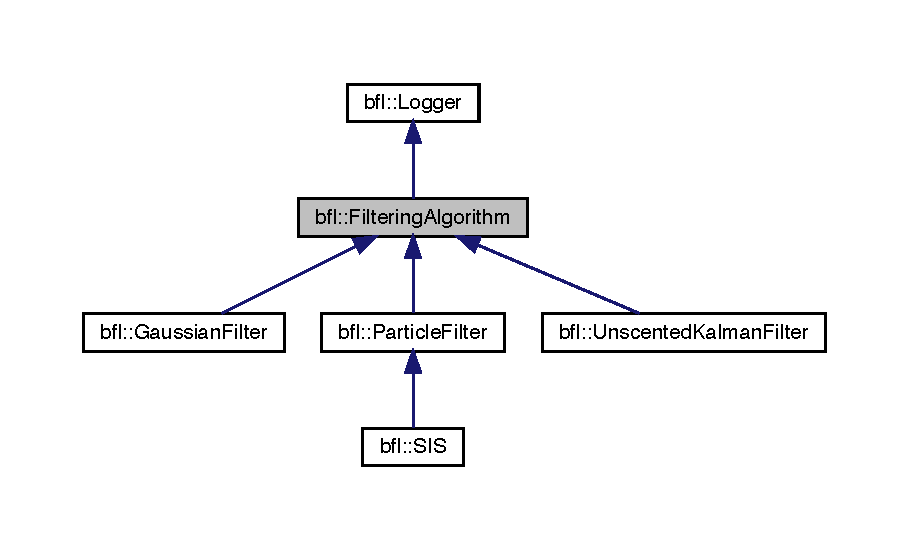
\includegraphics[width=350pt]{classbfl_1_1FilteringAlgorithm__inherit__graph}
\end{center}
\end{figure}
\subsection*{Public Member Functions}
\begin{DoxyCompactItemize}
\item 
virtual \mbox{\hyperlink{classbfl_1_1FilteringAlgorithm_ab286cc00b054717679fb13a3b709b1c4}{$\sim$\+Filtering\+Algorithm}} () noexcept
\item 
bool \mbox{\hyperlink{classbfl_1_1FilteringAlgorithm_a96651f8464190c0a56d79219a1017147}{boot}} ()
\item 
void \mbox{\hyperlink{classbfl_1_1FilteringAlgorithm_a009cbe5f4bbb16967f6c6ddcaed8fbb1}{run}} ()
\item 
bool \mbox{\hyperlink{classbfl_1_1FilteringAlgorithm_a40372c24fa050eb0274371172df0a244}{wait}} ()
\item 
void \mbox{\hyperlink{classbfl_1_1FilteringAlgorithm_a2403c62fbd7bd7f5cda56a84f5f30331}{reset}} ()
\item 
void \mbox{\hyperlink{classbfl_1_1FilteringAlgorithm_a6022859aa985474fb997343cc935b11e}{reboot}} ()
\item 
bool \mbox{\hyperlink{classbfl_1_1FilteringAlgorithm_a1dc912d89ee8f96d4f3e8209865c5308}{teardown}} ()
\item 
unsigned int \mbox{\hyperlink{classbfl_1_1FilteringAlgorithm_a8c43b1f3dac30934c0a03de348d4a29d}{get\+Filtering\+Step}} ()
\item 
bool \mbox{\hyperlink{classbfl_1_1FilteringAlgorithm_a5cfecab2c778620e2557237472bb1721}{is\+Running}} ()
\item 
virtual bool \mbox{\hyperlink{classbfl_1_1FilteringAlgorithm_ac8a718a614905d89d6a43bbbc70d68b2}{skip}} (const std\+::string \&what\+\_\+step, const bool status)=0
\item 
bool \mbox{\hyperlink{classbfl_1_1Logger_ae94b97b6e8d7902e8ce048384813122e}{enable\+\_\+log}} (const std\+::string \&prefix\+\_\+path, const std\+::string \&prefix\+\_\+name)
\item 
bool \mbox{\hyperlink{classbfl_1_1Logger_a440467a28ccc46490d767fe0ef6f556a}{disable\+\_\+log}} ()
\item 
std\+::string \mbox{\hyperlink{classbfl_1_1Logger_a56cf1a4e712bf23d9978420a8a59a62b}{get\+\_\+prefix\+\_\+path}} () const
\item 
std\+::string \mbox{\hyperlink{classbfl_1_1Logger_a913a795b7bfbf378815eeb342d68a7c0}{get\+\_\+prefix\+\_\+name}} () const
\item 
{\footnotesize template$<$typename Datum\+Type $>$ }\\void \mbox{\hyperlink{classbfl_1_1Logger_a1033ff31398484f2132f84fd140da9e3}{logger}} (Datum\+Type datum)
\item 
{\footnotesize template$<$typename... Data\+Type$>$ }\\void \mbox{\hyperlink{classbfl_1_1Logger_aca2086c9256e5c404872b91f7f25b97d}{logger}} (Data\+Type... data)
\item 
{\footnotesize template$<$typename Datum\+Type $>$ }\\void \mbox{\hyperlink{classbfl_1_1Logger_a50b1c109730fa98f66e66f420f0158fe}{logger}} (Datum\+Type datum) const
\item 
{\footnotesize template$<$typename... Data\+Type$>$ }\\void \mbox{\hyperlink{classbfl_1_1Logger_a0f0cf7ce956546d94dfb1feb7cebf171}{logger}} (Data\+Type... data) const
\end{DoxyCompactItemize}
\subsection*{Protected Member Functions}
\begin{DoxyCompactItemize}
\item 
virtual bool \mbox{\hyperlink{classbfl_1_1FilteringAlgorithm_adebe2ec2372f97a2a5baecf8c2c2a9c9}{initialization}} ()=0
\item 
virtual void \mbox{\hyperlink{classbfl_1_1FilteringAlgorithm_ab3bceb43b5810a4bf1da884b8a0b145a}{filtering\+Step}} ()=0
\item 
virtual bool \mbox{\hyperlink{classbfl_1_1FilteringAlgorithm_a5fc12882356f6906b102fbfff2bc4b7c}{run\+Condition}} ()=0
\item 
virtual std\+::vector$<$ std\+::string $>$ \mbox{\hyperlink{classbfl_1_1Logger_a328ceaa8e70e6918f11142b12b8be217}{log\+\_\+filenames}} (const std\+::string \&prefix\+\_\+path, const std\+::string \&prefix\+\_\+name)
\item 
virtual void \mbox{\hyperlink{classbfl_1_1Logger_ad44f46593cb8c4c87c1178eb326e2f64}{log}} ()
\end{DoxyCompactItemize}
\subsection*{Private Member Functions}
\begin{DoxyCompactItemize}
\item 
void \mbox{\hyperlink{classbfl_1_1FilteringAlgorithm_a139fe290f73939e72c88cb43c8ef7544}{filtering\+Recursion}} ()
\end{DoxyCompactItemize}
\subsection*{Private Attributes}
\begin{DoxyCompactItemize}
\item 
unsigned int \mbox{\hyperlink{classbfl_1_1FilteringAlgorithm_a1d08a5db263e415138d88c9a01535767}{filtering\+\_\+step\+\_\+}} = 0
\item 
std\+::thread \mbox{\hyperlink{classbfl_1_1FilteringAlgorithm_a2fa16711fd751628977afbbf9f7e9d6d}{filtering\+\_\+thread\+\_\+}}
\item 
std\+::mutex \mbox{\hyperlink{classbfl_1_1FilteringAlgorithm_a8983a40e915d3dbbc306d8f281ac449b}{mtx\+\_\+run\+\_\+}}
\item 
std\+::condition\+\_\+variable \mbox{\hyperlink{classbfl_1_1FilteringAlgorithm_ae92a6d82ce18c35516f42a7109c931af}{cv\+\_\+run\+\_\+}}
\item 
bool \mbox{\hyperlink{classbfl_1_1FilteringAlgorithm_a826eea2b551a2c2beab38394ed4c57c9}{run\+\_\+}} = false
\item 
bool \mbox{\hyperlink{classbfl_1_1FilteringAlgorithm_a4edf8ab29c4a1f8148ea276561299acb}{reset\+\_\+}} = false
\item 
bool \mbox{\hyperlink{classbfl_1_1FilteringAlgorithm_a3bc20cde7fc24767328f8a1ebd3e8cc8}{teardown\+\_\+}} = false
\end{DoxyCompactItemize}


\subsection{Detailed Description}


Definition at line 20 of file Filtering\+Algorithm.\+h.



\subsection{Constructor \& Destructor Documentation}
\mbox{\Hypertarget{classbfl_1_1FilteringAlgorithm_ab286cc00b054717679fb13a3b709b1c4}\label{classbfl_1_1FilteringAlgorithm_ab286cc00b054717679fb13a3b709b1c4}} 
\index{bfl\+::\+Filtering\+Algorithm@{bfl\+::\+Filtering\+Algorithm}!````~Filtering\+Algorithm@{$\sim$\+Filtering\+Algorithm}}
\index{````~Filtering\+Algorithm@{$\sim$\+Filtering\+Algorithm}!bfl\+::\+Filtering\+Algorithm@{bfl\+::\+Filtering\+Algorithm}}
\subsubsection{\texorpdfstring{$\sim$\+Filtering\+Algorithm()}{~FilteringAlgorithm()}}
{\footnotesize\ttfamily virtual bfl\+::\+Filtering\+Algorithm\+::$\sim$\+Filtering\+Algorithm (\begin{DoxyParamCaption}{ }\end{DoxyParamCaption})\hspace{0.3cm}{\ttfamily [inline]}, {\ttfamily [virtual]}, {\ttfamily [noexcept]}}



Definition at line 23 of file Filtering\+Algorithm.\+h.



\subsection{Member Function Documentation}
\mbox{\Hypertarget{classbfl_1_1FilteringAlgorithm_a96651f8464190c0a56d79219a1017147}\label{classbfl_1_1FilteringAlgorithm_a96651f8464190c0a56d79219a1017147}} 
\index{bfl\+::\+Filtering\+Algorithm@{bfl\+::\+Filtering\+Algorithm}!boot@{boot}}
\index{boot@{boot}!bfl\+::\+Filtering\+Algorithm@{bfl\+::\+Filtering\+Algorithm}}
\subsubsection{\texorpdfstring{boot()}{boot()}}
{\footnotesize\ttfamily bool Filtering\+Algorithm\+::boot (\begin{DoxyParamCaption}{ }\end{DoxyParamCaption})}



Definition at line 8 of file Filtering\+Algorithm.\+cpp.



References filtering\+\_\+thread\+\_\+, and filtering\+Recursion().

Here is the call graph for this function\+:
\nopagebreak
\begin{figure}[H]
\begin{center}
\leavevmode
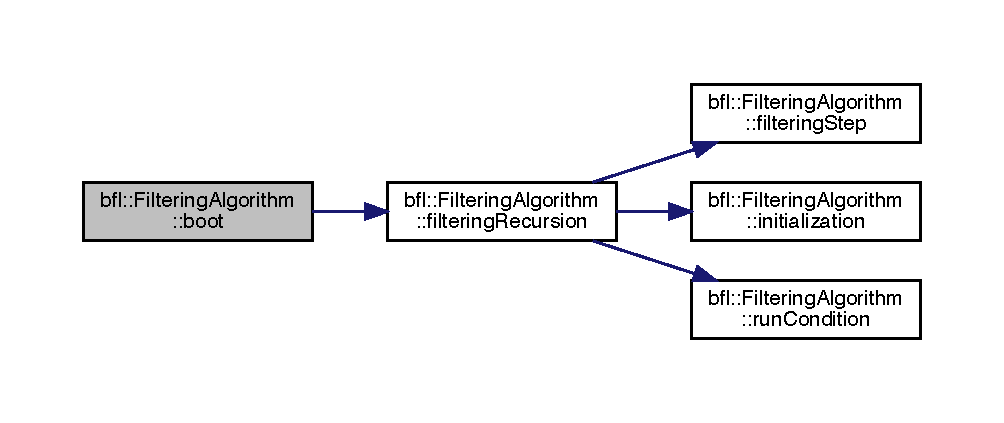
\includegraphics[width=350pt]{classbfl_1_1FilteringAlgorithm_a96651f8464190c0a56d79219a1017147_cgraph}
\end{center}
\end{figure}
\mbox{\Hypertarget{classbfl_1_1Logger_a440467a28ccc46490d767fe0ef6f556a}\label{classbfl_1_1Logger_a440467a28ccc46490d767fe0ef6f556a}} 
\index{bfl\+::\+Filtering\+Algorithm@{bfl\+::\+Filtering\+Algorithm}!disable\+\_\+log@{disable\+\_\+log}}
\index{disable\+\_\+log@{disable\+\_\+log}!bfl\+::\+Filtering\+Algorithm@{bfl\+::\+Filtering\+Algorithm}}
\subsubsection{\texorpdfstring{disable\+\_\+log()}{disable\_log()}}
{\footnotesize\ttfamily bool Logger\+::disable\+\_\+log (\begin{DoxyParamCaption}{ }\end{DoxyParamCaption})\hspace{0.3cm}{\ttfamily [inherited]}}



Definition at line 58 of file Logger.\+cpp.



References bfl\+::\+Logger\+::file\+\_\+names\+\_\+, bfl\+::\+Logger\+::log\+\_\+enabled\+\_\+, and bfl\+::\+Logger\+::log\+\_\+files\+\_\+.



Referenced by bfl\+::\+Logger\+::$\sim$\+Logger().

\mbox{\Hypertarget{classbfl_1_1Logger_ae94b97b6e8d7902e8ce048384813122e}\label{classbfl_1_1Logger_ae94b97b6e8d7902e8ce048384813122e}} 
\index{bfl\+::\+Filtering\+Algorithm@{bfl\+::\+Filtering\+Algorithm}!enable\+\_\+log@{enable\+\_\+log}}
\index{enable\+\_\+log@{enable\+\_\+log}!bfl\+::\+Filtering\+Algorithm@{bfl\+::\+Filtering\+Algorithm}}
\subsubsection{\texorpdfstring{enable\+\_\+log()}{enable\_log()}}
{\footnotesize\ttfamily bool Logger\+::enable\+\_\+log (\begin{DoxyParamCaption}\item[{const std\+::string \&}]{prefix\+\_\+path,  }\item[{const std\+::string \&}]{prefix\+\_\+name }\end{DoxyParamCaption})\hspace{0.3cm}{\ttfamily [inherited]}}



Definition at line 15 of file Logger.\+cpp.



References bfl\+::\+Logger\+::file\+\_\+names\+\_\+, bfl\+::\+Logger\+::log\+\_\+enabled\+\_\+, bfl\+::\+Logger\+::log\+\_\+filenames(), and bfl\+::\+Logger\+::log\+\_\+files\+\_\+.

Here is the call graph for this function\+:
\nopagebreak
\begin{figure}[H]
\begin{center}
\leavevmode
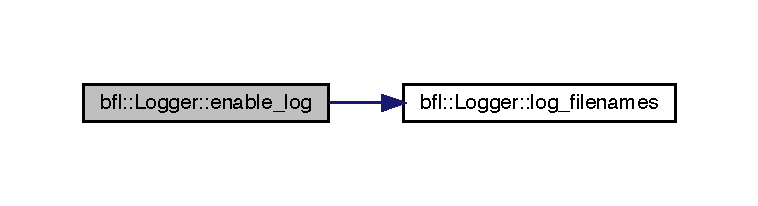
\includegraphics[width=350pt]{classbfl_1_1Logger_ae94b97b6e8d7902e8ce048384813122e_cgraph}
\end{center}
\end{figure}
\mbox{\Hypertarget{classbfl_1_1FilteringAlgorithm_a139fe290f73939e72c88cb43c8ef7544}\label{classbfl_1_1FilteringAlgorithm_a139fe290f73939e72c88cb43c8ef7544}} 
\index{bfl\+::\+Filtering\+Algorithm@{bfl\+::\+Filtering\+Algorithm}!filtering\+Recursion@{filtering\+Recursion}}
\index{filtering\+Recursion@{filtering\+Recursion}!bfl\+::\+Filtering\+Algorithm@{bfl\+::\+Filtering\+Algorithm}}
\subsubsection{\texorpdfstring{filtering\+Recursion()}{filteringRecursion()}}
{\footnotesize\ttfamily void Filtering\+Algorithm\+::filtering\+Recursion (\begin{DoxyParamCaption}{ }\end{DoxyParamCaption})\hspace{0.3cm}{\ttfamily [private]}}



Definition at line 95 of file Filtering\+Algorithm.\+cpp.



References cv\+\_\+run\+\_\+, filtering\+\_\+step\+\_\+, filtering\+Step(), initialization(), mtx\+\_\+run\+\_\+, reset\+\_\+, run\+\_\+, run\+Condition(), and teardown\+\_\+.



Referenced by boot().

Here is the call graph for this function\+:
\nopagebreak
\begin{figure}[H]
\begin{center}
\leavevmode
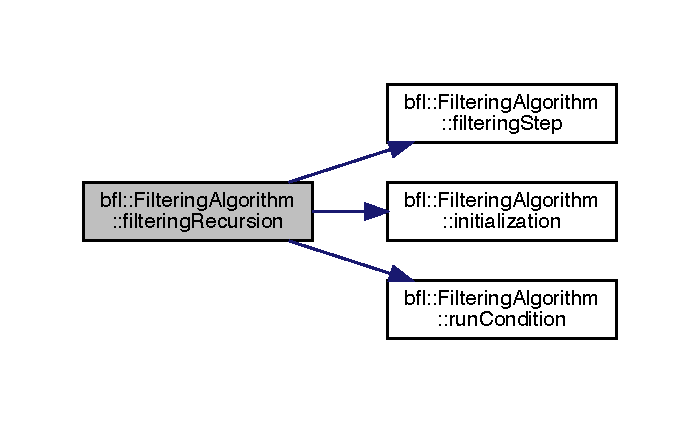
\includegraphics[width=336pt]{classbfl_1_1FilteringAlgorithm_a139fe290f73939e72c88cb43c8ef7544_cgraph}
\end{center}
\end{figure}
\mbox{\Hypertarget{classbfl_1_1FilteringAlgorithm_ab3bceb43b5810a4bf1da884b8a0b145a}\label{classbfl_1_1FilteringAlgorithm_ab3bceb43b5810a4bf1da884b8a0b145a}} 
\index{bfl\+::\+Filtering\+Algorithm@{bfl\+::\+Filtering\+Algorithm}!filtering\+Step@{filtering\+Step}}
\index{filtering\+Step@{filtering\+Step}!bfl\+::\+Filtering\+Algorithm@{bfl\+::\+Filtering\+Algorithm}}
\subsubsection{\texorpdfstring{filtering\+Step()}{filteringStep()}}
{\footnotesize\ttfamily virtual void bfl\+::\+Filtering\+Algorithm\+::filtering\+Step (\begin{DoxyParamCaption}{ }\end{DoxyParamCaption})\hspace{0.3cm}{\ttfamily [protected]}, {\ttfamily [pure virtual]}}



Implemented in \mbox{\hyperlink{classbfl_1_1SIS_a582f06cc5456d2cc6ed8f90087cbbb4c}{bfl\+::\+S\+IS}}, \mbox{\hyperlink{classbfl_1_1GaussianFilter_ae30a175454a93685eca79d3ef857f7bc}{bfl\+::\+Gaussian\+Filter}}, and \mbox{\hyperlink{classbfl_1_1UnscentedKalmanFilter_a169451bb711a03ad2dc28a40e3ad867f}{bfl\+::\+Unscented\+Kalman\+Filter}}.



Referenced by filtering\+Recursion().

\mbox{\Hypertarget{classbfl_1_1Logger_a913a795b7bfbf378815eeb342d68a7c0}\label{classbfl_1_1Logger_a913a795b7bfbf378815eeb342d68a7c0}} 
\index{bfl\+::\+Filtering\+Algorithm@{bfl\+::\+Filtering\+Algorithm}!get\+\_\+prefix\+\_\+name@{get\+\_\+prefix\+\_\+name}}
\index{get\+\_\+prefix\+\_\+name@{get\+\_\+prefix\+\_\+name}!bfl\+::\+Filtering\+Algorithm@{bfl\+::\+Filtering\+Algorithm}}
\subsubsection{\texorpdfstring{get\+\_\+prefix\+\_\+name()}{get\_prefix\_name()}}
{\footnotesize\ttfamily std\+::string Logger\+::get\+\_\+prefix\+\_\+name (\begin{DoxyParamCaption}{ }\end{DoxyParamCaption}) const\hspace{0.3cm}{\ttfamily [inherited]}}



Definition at line 81 of file Logger.\+cpp.



References bfl\+::\+Logger\+::prefix\+\_\+name\+\_\+.

\mbox{\Hypertarget{classbfl_1_1Logger_a56cf1a4e712bf23d9978420a8a59a62b}\label{classbfl_1_1Logger_a56cf1a4e712bf23d9978420a8a59a62b}} 
\index{bfl\+::\+Filtering\+Algorithm@{bfl\+::\+Filtering\+Algorithm}!get\+\_\+prefix\+\_\+path@{get\+\_\+prefix\+\_\+path}}
\index{get\+\_\+prefix\+\_\+path@{get\+\_\+prefix\+\_\+path}!bfl\+::\+Filtering\+Algorithm@{bfl\+::\+Filtering\+Algorithm}}
\subsubsection{\texorpdfstring{get\+\_\+prefix\+\_\+path()}{get\_prefix\_path()}}
{\footnotesize\ttfamily std\+::string Logger\+::get\+\_\+prefix\+\_\+path (\begin{DoxyParamCaption}{ }\end{DoxyParamCaption}) const\hspace{0.3cm}{\ttfamily [inherited]}}



Definition at line 75 of file Logger.\+cpp.



References bfl\+::\+Logger\+::prefix\+\_\+path\+\_\+.

\mbox{\Hypertarget{classbfl_1_1FilteringAlgorithm_a8c43b1f3dac30934c0a03de348d4a29d}\label{classbfl_1_1FilteringAlgorithm_a8c43b1f3dac30934c0a03de348d4a29d}} 
\index{bfl\+::\+Filtering\+Algorithm@{bfl\+::\+Filtering\+Algorithm}!get\+Filtering\+Step@{get\+Filtering\+Step}}
\index{get\+Filtering\+Step@{get\+Filtering\+Step}!bfl\+::\+Filtering\+Algorithm@{bfl\+::\+Filtering\+Algorithm}}
\subsubsection{\texorpdfstring{get\+Filtering\+Step()}{getFilteringStep()}}
{\footnotesize\ttfamily unsigned int Filtering\+Algorithm\+::get\+Filtering\+Step (\begin{DoxyParamCaption}{ }\end{DoxyParamCaption})}



Definition at line 83 of file Filtering\+Algorithm.\+cpp.



References filtering\+\_\+step\+\_\+.

\mbox{\Hypertarget{classbfl_1_1FilteringAlgorithm_adebe2ec2372f97a2a5baecf8c2c2a9c9}\label{classbfl_1_1FilteringAlgorithm_adebe2ec2372f97a2a5baecf8c2c2a9c9}} 
\index{bfl\+::\+Filtering\+Algorithm@{bfl\+::\+Filtering\+Algorithm}!initialization@{initialization}}
\index{initialization@{initialization}!bfl\+::\+Filtering\+Algorithm@{bfl\+::\+Filtering\+Algorithm}}
\subsubsection{\texorpdfstring{initialization()}{initialization()}}
{\footnotesize\ttfamily virtual bool bfl\+::\+Filtering\+Algorithm\+::initialization (\begin{DoxyParamCaption}{ }\end{DoxyParamCaption})\hspace{0.3cm}{\ttfamily [protected]}, {\ttfamily [pure virtual]}}



Implemented in \mbox{\hyperlink{classbfl_1_1SIS_a59e4f35fc05d2088e6dc13d622cafd1d}{bfl\+::\+S\+IS}}, \mbox{\hyperlink{classbfl_1_1GaussianFilter_ac0305fa835af89ba5962ee1211d4d0c0}{bfl\+::\+Gaussian\+Filter}}, and \mbox{\hyperlink{classbfl_1_1UnscentedKalmanFilter_ad221e4abd58c2e67e9b44f52a0c9504f}{bfl\+::\+Unscented\+Kalman\+Filter}}.



Referenced by filtering\+Recursion().

\mbox{\Hypertarget{classbfl_1_1FilteringAlgorithm_a5cfecab2c778620e2557237472bb1721}\label{classbfl_1_1FilteringAlgorithm_a5cfecab2c778620e2557237472bb1721}} 
\index{bfl\+::\+Filtering\+Algorithm@{bfl\+::\+Filtering\+Algorithm}!is\+Running@{is\+Running}}
\index{is\+Running@{is\+Running}!bfl\+::\+Filtering\+Algorithm@{bfl\+::\+Filtering\+Algorithm}}
\subsubsection{\texorpdfstring{is\+Running()}{isRunning()}}
{\footnotesize\ttfamily bool Filtering\+Algorithm\+::is\+Running (\begin{DoxyParamCaption}{ }\end{DoxyParamCaption})}



Definition at line 89 of file Filtering\+Algorithm.\+cpp.



References run\+\_\+.

\mbox{\Hypertarget{classbfl_1_1Logger_ad44f46593cb8c4c87c1178eb326e2f64}\label{classbfl_1_1Logger_ad44f46593cb8c4c87c1178eb326e2f64}} 
\index{bfl\+::\+Filtering\+Algorithm@{bfl\+::\+Filtering\+Algorithm}!log@{log}}
\index{log@{log}!bfl\+::\+Filtering\+Algorithm@{bfl\+::\+Filtering\+Algorithm}}
\subsubsection{\texorpdfstring{log()}{log()}}
{\footnotesize\ttfamily void Logger\+::log (\begin{DoxyParamCaption}{ }\end{DoxyParamCaption})\hspace{0.3cm}{\ttfamily [protected]}, {\ttfamily [virtual]}, {\ttfamily [inherited]}}



Reimplemented in \mbox{\hyperlink{classbfl_1_1SIS_aeb0b87af1cc1fc4b616989ef489ecccc}{bfl\+::\+S\+IS}}, \mbox{\hyperlink{classbfl_1_1SimulatedStateModel_aa022eb0d50d898ffcc831af2907265b2}{bfl\+::\+Simulated\+State\+Model}}, and \mbox{\hyperlink{classbfl_1_1SimulatedLinearSensor_ab75bbe744d8516c97dfc90ad499b10e6}{bfl\+::\+Simulated\+Linear\+Sensor}}.



Definition at line 99 of file Logger.\+cpp.



Referenced by bfl\+::\+Gaussian\+Filter\+::filtering\+Step().

\mbox{\Hypertarget{classbfl_1_1Logger_a328ceaa8e70e6918f11142b12b8be217}\label{classbfl_1_1Logger_a328ceaa8e70e6918f11142b12b8be217}} 
\index{bfl\+::\+Filtering\+Algorithm@{bfl\+::\+Filtering\+Algorithm}!log\+\_\+filenames@{log\+\_\+filenames}}
\index{log\+\_\+filenames@{log\+\_\+filenames}!bfl\+::\+Filtering\+Algorithm@{bfl\+::\+Filtering\+Algorithm}}
\subsubsection{\texorpdfstring{log\+\_\+filenames()}{log\_filenames()}}
{\footnotesize\ttfamily std\+::vector$<$ std\+::string $>$ Logger\+::log\+\_\+filenames (\begin{DoxyParamCaption}\item[{const std\+::string \&}]{prefix\+\_\+path,  }\item[{const std\+::string \&}]{prefix\+\_\+name }\end{DoxyParamCaption})\hspace{0.3cm}{\ttfamily [protected]}, {\ttfamily [virtual]}, {\ttfamily [inherited]}}



Reimplemented in \mbox{\hyperlink{classbfl_1_1LinearModel_a8b8f645a7b7d8ebbb02c8958428fcf10}{bfl\+::\+Linear\+Model}}, \mbox{\hyperlink{classbfl_1_1SimulatedStateModel_ab4212871b8ca425855ec351c13dc3052}{bfl\+::\+Simulated\+State\+Model}}, and \mbox{\hyperlink{classbfl_1_1SIS_a805aef60946bfcaae4f65473dc7bd5ae}{bfl\+::\+S\+IS}}.



Definition at line 87 of file Logger.\+cpp.



Referenced by bfl\+::\+Logger\+::enable\+\_\+log().

\mbox{\Hypertarget{classbfl_1_1Logger_a1033ff31398484f2132f84fd140da9e3}\label{classbfl_1_1Logger_a1033ff31398484f2132f84fd140da9e3}} 
\index{bfl\+::\+Filtering\+Algorithm@{bfl\+::\+Filtering\+Algorithm}!logger@{logger}}
\index{logger@{logger}!bfl\+::\+Filtering\+Algorithm@{bfl\+::\+Filtering\+Algorithm}}
\subsubsection{\texorpdfstring{logger()}{logger()}\hspace{0.1cm}{\footnotesize\ttfamily [1/4]}}
{\footnotesize\ttfamily template$<$typename Datum\+Type $>$ \\
void bfl\+::\+Logger\+::logger (\begin{DoxyParamCaption}\item[{Datum\+Type}]{datum }\end{DoxyParamCaption})\hspace{0.3cm}{\ttfamily [inline]}, {\ttfamily [inherited]}}



Definition at line 28 of file Logger.\+h.



References bfl\+::\+Logger\+::log\+\_\+enabled\+\_\+, and bfl\+::\+Logger\+::log\+\_\+files\+\_\+.



Referenced by bfl\+::\+Simulated\+Linear\+Sensor\+::log().

\mbox{\Hypertarget{classbfl_1_1Logger_aca2086c9256e5c404872b91f7f25b97d}\label{classbfl_1_1Logger_aca2086c9256e5c404872b91f7f25b97d}} 
\index{bfl\+::\+Filtering\+Algorithm@{bfl\+::\+Filtering\+Algorithm}!logger@{logger}}
\index{logger@{logger}!bfl\+::\+Filtering\+Algorithm@{bfl\+::\+Filtering\+Algorithm}}
\subsubsection{\texorpdfstring{logger()}{logger()}\hspace{0.1cm}{\footnotesize\ttfamily [2/4]}}
{\footnotesize\ttfamily template$<$typename... Data\+Type$>$ \\
void bfl\+::\+Logger\+::logger (\begin{DoxyParamCaption}\item[{Data\+Type...}]{data }\end{DoxyParamCaption})\hspace{0.3cm}{\ttfamily [inline]}, {\ttfamily [inherited]}}



Definition at line 35 of file Logger.\+h.



References bfl\+::\+Logger\+::log\+\_\+enabled\+\_\+, and bfl\+::\+Logger\+::logger\+\_\+helper().

Here is the call graph for this function\+:
\nopagebreak
\begin{figure}[H]
\begin{center}
\leavevmode
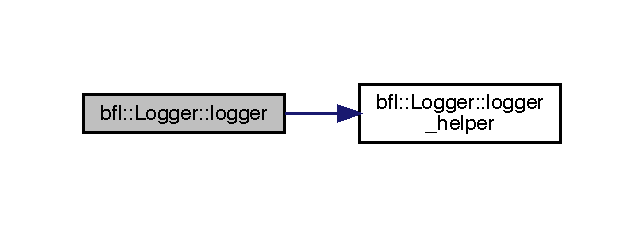
\includegraphics[width=309pt]{classbfl_1_1Logger_aca2086c9256e5c404872b91f7f25b97d_cgraph}
\end{center}
\end{figure}
\mbox{\Hypertarget{classbfl_1_1Logger_a50b1c109730fa98f66e66f420f0158fe}\label{classbfl_1_1Logger_a50b1c109730fa98f66e66f420f0158fe}} 
\index{bfl\+::\+Filtering\+Algorithm@{bfl\+::\+Filtering\+Algorithm}!logger@{logger}}
\index{logger@{logger}!bfl\+::\+Filtering\+Algorithm@{bfl\+::\+Filtering\+Algorithm}}
\subsubsection{\texorpdfstring{logger()}{logger()}\hspace{0.1cm}{\footnotesize\ttfamily [3/4]}}
{\footnotesize\ttfamily template$<$typename Datum\+Type $>$ \\
void bfl\+::\+Logger\+::logger (\begin{DoxyParamCaption}\item[{Datum\+Type}]{datum }\end{DoxyParamCaption}) const\hspace{0.3cm}{\ttfamily [inline]}, {\ttfamily [inherited]}}



Definition at line 42 of file Logger.\+h.



References bfl\+::\+Logger\+::log\+\_\+enabled\+\_\+, and bfl\+::\+Logger\+::log\+\_\+files\+\_\+.

\mbox{\Hypertarget{classbfl_1_1Logger_a0f0cf7ce956546d94dfb1feb7cebf171}\label{classbfl_1_1Logger_a0f0cf7ce956546d94dfb1feb7cebf171}} 
\index{bfl\+::\+Filtering\+Algorithm@{bfl\+::\+Filtering\+Algorithm}!logger@{logger}}
\index{logger@{logger}!bfl\+::\+Filtering\+Algorithm@{bfl\+::\+Filtering\+Algorithm}}
\subsubsection{\texorpdfstring{logger()}{logger()}\hspace{0.1cm}{\footnotesize\ttfamily [4/4]}}
{\footnotesize\ttfamily template$<$typename... Data\+Type$>$ \\
void bfl\+::\+Logger\+::logger (\begin{DoxyParamCaption}\item[{Data\+Type...}]{data }\end{DoxyParamCaption}) const\hspace{0.3cm}{\ttfamily [inline]}, {\ttfamily [inherited]}}



Definition at line 49 of file Logger.\+h.



References bfl\+::\+Logger\+::log\+\_\+enabled\+\_\+, and bfl\+::\+Logger\+::logger\+\_\+helper().

Here is the call graph for this function\+:
\nopagebreak
\begin{figure}[H]
\begin{center}
\leavevmode
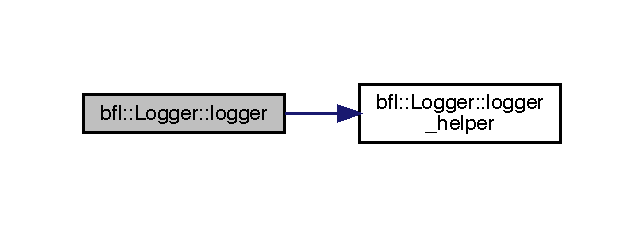
\includegraphics[width=309pt]{classbfl_1_1Logger_a0f0cf7ce956546d94dfb1feb7cebf171_cgraph}
\end{center}
\end{figure}
\mbox{\Hypertarget{classbfl_1_1FilteringAlgorithm_a6022859aa985474fb997343cc935b11e}\label{classbfl_1_1FilteringAlgorithm_a6022859aa985474fb997343cc935b11e}} 
\index{bfl\+::\+Filtering\+Algorithm@{bfl\+::\+Filtering\+Algorithm}!reboot@{reboot}}
\index{reboot@{reboot}!bfl\+::\+Filtering\+Algorithm@{bfl\+::\+Filtering\+Algorithm}}
\subsubsection{\texorpdfstring{reboot()}{reboot()}}
{\footnotesize\ttfamily void Filtering\+Algorithm\+::reboot (\begin{DoxyParamCaption}{ }\end{DoxyParamCaption})}



Definition at line 66 of file Filtering\+Algorithm.\+cpp.



References cv\+\_\+run\+\_\+, mtx\+\_\+run\+\_\+, reset\+\_\+, and run\+\_\+.

\mbox{\Hypertarget{classbfl_1_1FilteringAlgorithm_a2403c62fbd7bd7f5cda56a84f5f30331}\label{classbfl_1_1FilteringAlgorithm_a2403c62fbd7bd7f5cda56a84f5f30331}} 
\index{bfl\+::\+Filtering\+Algorithm@{bfl\+::\+Filtering\+Algorithm}!reset@{reset}}
\index{reset@{reset}!bfl\+::\+Filtering\+Algorithm@{bfl\+::\+Filtering\+Algorithm}}
\subsubsection{\texorpdfstring{reset()}{reset()}}
{\footnotesize\ttfamily void Filtering\+Algorithm\+::reset (\begin{DoxyParamCaption}{ }\end{DoxyParamCaption})}



Definition at line 60 of file Filtering\+Algorithm.\+cpp.



References reset\+\_\+.

\mbox{\Hypertarget{classbfl_1_1FilteringAlgorithm_a009cbe5f4bbb16967f6c6ddcaed8fbb1}\label{classbfl_1_1FilteringAlgorithm_a009cbe5f4bbb16967f6c6ddcaed8fbb1}} 
\index{bfl\+::\+Filtering\+Algorithm@{bfl\+::\+Filtering\+Algorithm}!run@{run}}
\index{run@{run}!bfl\+::\+Filtering\+Algorithm@{bfl\+::\+Filtering\+Algorithm}}
\subsubsection{\texorpdfstring{run()}{run()}}
{\footnotesize\ttfamily void Filtering\+Algorithm\+::run (\begin{DoxyParamCaption}{ }\end{DoxyParamCaption})}



Definition at line 26 of file Filtering\+Algorithm.\+cpp.



References cv\+\_\+run\+\_\+, mtx\+\_\+run\+\_\+, and run\+\_\+.

\mbox{\Hypertarget{classbfl_1_1FilteringAlgorithm_a5fc12882356f6906b102fbfff2bc4b7c}\label{classbfl_1_1FilteringAlgorithm_a5fc12882356f6906b102fbfff2bc4b7c}} 
\index{bfl\+::\+Filtering\+Algorithm@{bfl\+::\+Filtering\+Algorithm}!run\+Condition@{run\+Condition}}
\index{run\+Condition@{run\+Condition}!bfl\+::\+Filtering\+Algorithm@{bfl\+::\+Filtering\+Algorithm}}
\subsubsection{\texorpdfstring{run\+Condition()}{runCondition()}}
{\footnotesize\ttfamily virtual bool bfl\+::\+Filtering\+Algorithm\+::run\+Condition (\begin{DoxyParamCaption}{ }\end{DoxyParamCaption})\hspace{0.3cm}{\ttfamily [protected]}, {\ttfamily [pure virtual]}}



Implemented in \mbox{\hyperlink{classbfl_1_1SIS_a669ac8eb19f6797f2735b94074727e8f}{bfl\+::\+S\+IS}}, and \mbox{\hyperlink{classbfl_1_1GaussianFilter_acf6902f6156c573560b57f10c1992b8a}{bfl\+::\+Gaussian\+Filter}}.



Referenced by filtering\+Recursion().

\mbox{\Hypertarget{classbfl_1_1FilteringAlgorithm_ac8a718a614905d89d6a43bbbc70d68b2}\label{classbfl_1_1FilteringAlgorithm_ac8a718a614905d89d6a43bbbc70d68b2}} 
\index{bfl\+::\+Filtering\+Algorithm@{bfl\+::\+Filtering\+Algorithm}!skip@{skip}}
\index{skip@{skip}!bfl\+::\+Filtering\+Algorithm@{bfl\+::\+Filtering\+Algorithm}}
\subsubsection{\texorpdfstring{skip()}{skip()}}
{\footnotesize\ttfamily virtual bool bfl\+::\+Filtering\+Algorithm\+::skip (\begin{DoxyParamCaption}\item[{const std\+::string \&}]{what\+\_\+step,  }\item[{const bool}]{status }\end{DoxyParamCaption})\hspace{0.3cm}{\ttfamily [pure virtual]}}



Implemented in \mbox{\hyperlink{classbfl_1_1GaussianFilter_a3ca79ee1451863d898baeea6a74ababd}{bfl\+::\+Gaussian\+Filter}}, and \mbox{\hyperlink{classbfl_1_1ParticleFilter_a2d7a5e7aaad179037273d35be229056d}{bfl\+::\+Particle\+Filter}}.

\mbox{\Hypertarget{classbfl_1_1FilteringAlgorithm_a1dc912d89ee8f96d4f3e8209865c5308}\label{classbfl_1_1FilteringAlgorithm_a1dc912d89ee8f96d4f3e8209865c5308}} 
\index{bfl\+::\+Filtering\+Algorithm@{bfl\+::\+Filtering\+Algorithm}!teardown@{teardown}}
\index{teardown@{teardown}!bfl\+::\+Filtering\+Algorithm@{bfl\+::\+Filtering\+Algorithm}}
\subsubsection{\texorpdfstring{teardown()}{teardown()}}
{\footnotesize\ttfamily bool Filtering\+Algorithm\+::teardown (\begin{DoxyParamCaption}{ }\end{DoxyParamCaption})}



Definition at line 75 of file Filtering\+Algorithm.\+cpp.



References teardown\+\_\+.

\mbox{\Hypertarget{classbfl_1_1FilteringAlgorithm_a40372c24fa050eb0274371172df0a244}\label{classbfl_1_1FilteringAlgorithm_a40372c24fa050eb0274371172df0a244}} 
\index{bfl\+::\+Filtering\+Algorithm@{bfl\+::\+Filtering\+Algorithm}!wait@{wait}}
\index{wait@{wait}!bfl\+::\+Filtering\+Algorithm@{bfl\+::\+Filtering\+Algorithm}}
\subsubsection{\texorpdfstring{wait()}{wait()}}
{\footnotesize\ttfamily bool Filtering\+Algorithm\+::wait (\begin{DoxyParamCaption}{ }\end{DoxyParamCaption})}



Definition at line 34 of file Filtering\+Algorithm.\+cpp.



References filtering\+\_\+thread\+\_\+.



\subsection{Member Data Documentation}
\mbox{\Hypertarget{classbfl_1_1FilteringAlgorithm_ae92a6d82ce18c35516f42a7109c931af}\label{classbfl_1_1FilteringAlgorithm_ae92a6d82ce18c35516f42a7109c931af}} 
\index{bfl\+::\+Filtering\+Algorithm@{bfl\+::\+Filtering\+Algorithm}!cv\+\_\+run\+\_\+@{cv\+\_\+run\+\_\+}}
\index{cv\+\_\+run\+\_\+@{cv\+\_\+run\+\_\+}!bfl\+::\+Filtering\+Algorithm@{bfl\+::\+Filtering\+Algorithm}}
\subsubsection{\texorpdfstring{cv\+\_\+run\+\_\+}{cv\_run\_}}
{\footnotesize\ttfamily std\+::condition\+\_\+variable bfl\+::\+Filtering\+Algorithm\+::cv\+\_\+run\+\_\+\hspace{0.3cm}{\ttfamily [private]}}



Definition at line 59 of file Filtering\+Algorithm.\+h.



Referenced by filtering\+Recursion(), reboot(), and run().

\mbox{\Hypertarget{classbfl_1_1FilteringAlgorithm_a1d08a5db263e415138d88c9a01535767}\label{classbfl_1_1FilteringAlgorithm_a1d08a5db263e415138d88c9a01535767}} 
\index{bfl\+::\+Filtering\+Algorithm@{bfl\+::\+Filtering\+Algorithm}!filtering\+\_\+step\+\_\+@{filtering\+\_\+step\+\_\+}}
\index{filtering\+\_\+step\+\_\+@{filtering\+\_\+step\+\_\+}!bfl\+::\+Filtering\+Algorithm@{bfl\+::\+Filtering\+Algorithm}}
\subsubsection{\texorpdfstring{filtering\+\_\+step\+\_\+}{filtering\_step\_}}
{\footnotesize\ttfamily unsigned int bfl\+::\+Filtering\+Algorithm\+::filtering\+\_\+step\+\_\+ = 0\hspace{0.3cm}{\ttfamily [private]}}



Definition at line 51 of file Filtering\+Algorithm.\+h.



Referenced by filtering\+Recursion(), and get\+Filtering\+Step().

\mbox{\Hypertarget{classbfl_1_1FilteringAlgorithm_a2fa16711fd751628977afbbf9f7e9d6d}\label{classbfl_1_1FilteringAlgorithm_a2fa16711fd751628977afbbf9f7e9d6d}} 
\index{bfl\+::\+Filtering\+Algorithm@{bfl\+::\+Filtering\+Algorithm}!filtering\+\_\+thread\+\_\+@{filtering\+\_\+thread\+\_\+}}
\index{filtering\+\_\+thread\+\_\+@{filtering\+\_\+thread\+\_\+}!bfl\+::\+Filtering\+Algorithm@{bfl\+::\+Filtering\+Algorithm}}
\subsubsection{\texorpdfstring{filtering\+\_\+thread\+\_\+}{filtering\_thread\_}}
{\footnotesize\ttfamily std\+::thread bfl\+::\+Filtering\+Algorithm\+::filtering\+\_\+thread\+\_\+\hspace{0.3cm}{\ttfamily [private]}}



Definition at line 53 of file Filtering\+Algorithm.\+h.



Referenced by boot(), and wait().

\mbox{\Hypertarget{classbfl_1_1FilteringAlgorithm_a8983a40e915d3dbbc306d8f281ac449b}\label{classbfl_1_1FilteringAlgorithm_a8983a40e915d3dbbc306d8f281ac449b}} 
\index{bfl\+::\+Filtering\+Algorithm@{bfl\+::\+Filtering\+Algorithm}!mtx\+\_\+run\+\_\+@{mtx\+\_\+run\+\_\+}}
\index{mtx\+\_\+run\+\_\+@{mtx\+\_\+run\+\_\+}!bfl\+::\+Filtering\+Algorithm@{bfl\+::\+Filtering\+Algorithm}}
\subsubsection{\texorpdfstring{mtx\+\_\+run\+\_\+}{mtx\_run\_}}
{\footnotesize\ttfamily std\+::mutex bfl\+::\+Filtering\+Algorithm\+::mtx\+\_\+run\+\_\+\hspace{0.3cm}{\ttfamily [private]}}



Definition at line 57 of file Filtering\+Algorithm.\+h.



Referenced by filtering\+Recursion(), reboot(), and run().

\mbox{\Hypertarget{classbfl_1_1FilteringAlgorithm_a4edf8ab29c4a1f8148ea276561299acb}\label{classbfl_1_1FilteringAlgorithm_a4edf8ab29c4a1f8148ea276561299acb}} 
\index{bfl\+::\+Filtering\+Algorithm@{bfl\+::\+Filtering\+Algorithm}!reset\+\_\+@{reset\+\_\+}}
\index{reset\+\_\+@{reset\+\_\+}!bfl\+::\+Filtering\+Algorithm@{bfl\+::\+Filtering\+Algorithm}}
\subsubsection{\texorpdfstring{reset\+\_\+}{reset\_}}
{\footnotesize\ttfamily bool bfl\+::\+Filtering\+Algorithm\+::reset\+\_\+ = false\hspace{0.3cm}{\ttfamily [private]}}



Definition at line 63 of file Filtering\+Algorithm.\+h.



Referenced by filtering\+Recursion(), reboot(), and reset().

\mbox{\Hypertarget{classbfl_1_1FilteringAlgorithm_a826eea2b551a2c2beab38394ed4c57c9}\label{classbfl_1_1FilteringAlgorithm_a826eea2b551a2c2beab38394ed4c57c9}} 
\index{bfl\+::\+Filtering\+Algorithm@{bfl\+::\+Filtering\+Algorithm}!run\+\_\+@{run\+\_\+}}
\index{run\+\_\+@{run\+\_\+}!bfl\+::\+Filtering\+Algorithm@{bfl\+::\+Filtering\+Algorithm}}
\subsubsection{\texorpdfstring{run\+\_\+}{run\_}}
{\footnotesize\ttfamily bool bfl\+::\+Filtering\+Algorithm\+::run\+\_\+ = false\hspace{0.3cm}{\ttfamily [private]}}



Definition at line 61 of file Filtering\+Algorithm.\+h.



Referenced by filtering\+Recursion(), is\+Running(), reboot(), and run().

\mbox{\Hypertarget{classbfl_1_1FilteringAlgorithm_a3bc20cde7fc24767328f8a1ebd3e8cc8}\label{classbfl_1_1FilteringAlgorithm_a3bc20cde7fc24767328f8a1ebd3e8cc8}} 
\index{bfl\+::\+Filtering\+Algorithm@{bfl\+::\+Filtering\+Algorithm}!teardown\+\_\+@{teardown\+\_\+}}
\index{teardown\+\_\+@{teardown\+\_\+}!bfl\+::\+Filtering\+Algorithm@{bfl\+::\+Filtering\+Algorithm}}
\subsubsection{\texorpdfstring{teardown\+\_\+}{teardown\_}}
{\footnotesize\ttfamily bool bfl\+::\+Filtering\+Algorithm\+::teardown\+\_\+ = false\hspace{0.3cm}{\ttfamily [private]}}



Definition at line 65 of file Filtering\+Algorithm.\+h.



Referenced by filtering\+Recursion(), and teardown().



The documentation for this class was generated from the following files\+:\begin{DoxyCompactItemize}
\item 
/\+Users/\+Claudio/\+Git\+Hub/bayes-\/filters-\/lib/src/\+Bayes\+Filters/include/\+Bayes\+Filters/\mbox{\hyperlink{FilteringAlgorithm_8h}{Filtering\+Algorithm.\+h}}\item 
/\+Users/\+Claudio/\+Git\+Hub/bayes-\/filters-\/lib/src/\+Bayes\+Filters/src/\mbox{\hyperlink{FilteringAlgorithm_8cpp}{Filtering\+Algorithm.\+cpp}}\end{DoxyCompactItemize}

\hypertarget{classbfl_1_1FilteringContext}{}\section{bfl\+:\+:Filtering\+Context Class Reference}
\label{classbfl_1_1FilteringContext}\index{bfl\+::\+Filtering\+Context@{bfl\+::\+Filtering\+Context}}


{\ttfamily \#include $<$Filtering\+Context.\+h$>$}

\subsection*{Public Member Functions}
\begin{DoxyCompactItemize}
\item 
\mbox{\hyperlink{classbfl_1_1FilteringContext_a55257440dbb1d21d10cd2a114333305c}{Filtering\+Context}} (std\+::shared\+\_\+ptr$<$ \mbox{\hyperlink{classbfl_1_1FilteringAlgorithm}{Filtering\+Algorithm}} $>$ filter)
\item 
virtual \mbox{\hyperlink{classbfl_1_1FilteringContext_a205a6c269a11dd7a2425753336b4416d}{$\sim$\+Filtering\+Context}} ()
\item 
void \mbox{\hyperlink{classbfl_1_1FilteringContext_ae231d933d38221f3505c7dcaef4d853a}{run}} ()
\item 
void \mbox{\hyperlink{classbfl_1_1FilteringContext_a77f5148a9365e4257554b1594cb45c8e}{save\+Result}} ()
\item 
void \mbox{\hyperlink{classbfl_1_1FilteringContext_a21b4c61a64a36aff518200aac5031d45}{set\+Parameter}} ()
\end{DoxyCompactItemize}
\subsection*{Private Attributes}
\begin{DoxyCompactItemize}
\item 
std\+::shared\+\_\+ptr$<$ \mbox{\hyperlink{classbfl_1_1FilteringAlgorithm}{Filtering\+Algorithm}} $>$ \mbox{\hyperlink{classbfl_1_1FilteringContext_a143316c648445254fdd512f317a81d5e}{filter\+\_\+}}
\end{DoxyCompactItemize}


\subsection{Detailed Description}


Definition at line 13 of file Filtering\+Context.\+h.



\subsection{Constructor \& Destructor Documentation}
\mbox{\Hypertarget{classbfl_1_1FilteringContext_a55257440dbb1d21d10cd2a114333305c}\label{classbfl_1_1FilteringContext_a55257440dbb1d21d10cd2a114333305c}} 
\index{bfl\+::\+Filtering\+Context@{bfl\+::\+Filtering\+Context}!Filtering\+Context@{Filtering\+Context}}
\index{Filtering\+Context@{Filtering\+Context}!bfl\+::\+Filtering\+Context@{bfl\+::\+Filtering\+Context}}
\subsubsection{\texorpdfstring{Filtering\+Context()}{FilteringContext()}}
{\footnotesize\ttfamily Filtering\+Context\+::\+Filtering\+Context (\begin{DoxyParamCaption}\item[{std\+::shared\+\_\+ptr$<$ \mbox{\hyperlink{classbfl_1_1FilteringAlgorithm}{Filtering\+Algorithm}} $>$}]{filter }\end{DoxyParamCaption})}



Definition at line 6 of file Filtering\+Context.\+cpp.

\mbox{\Hypertarget{classbfl_1_1FilteringContext_a205a6c269a11dd7a2425753336b4416d}\label{classbfl_1_1FilteringContext_a205a6c269a11dd7a2425753336b4416d}} 
\index{bfl\+::\+Filtering\+Context@{bfl\+::\+Filtering\+Context}!````~Filtering\+Context@{$\sim$\+Filtering\+Context}}
\index{````~Filtering\+Context@{$\sim$\+Filtering\+Context}!bfl\+::\+Filtering\+Context@{bfl\+::\+Filtering\+Context}}
\subsubsection{\texorpdfstring{$\sim$\+Filtering\+Context()}{~FilteringContext()}}
{\footnotesize\ttfamily Filtering\+Context\+::$\sim$\+Filtering\+Context (\begin{DoxyParamCaption}{ }\end{DoxyParamCaption})\hspace{0.3cm}{\ttfamily [virtual]}}



Definition at line 9 of file Filtering\+Context.\+cpp.



\subsection{Member Function Documentation}
\mbox{\Hypertarget{classbfl_1_1FilteringContext_ae231d933d38221f3505c7dcaef4d853a}\label{classbfl_1_1FilteringContext_ae231d933d38221f3505c7dcaef4d853a}} 
\index{bfl\+::\+Filtering\+Context@{bfl\+::\+Filtering\+Context}!run@{run}}
\index{run@{run}!bfl\+::\+Filtering\+Context@{bfl\+::\+Filtering\+Context}}
\subsubsection{\texorpdfstring{run()}{run()}}
{\footnotesize\ttfamily void Filtering\+Context\+::run (\begin{DoxyParamCaption}{ }\end{DoxyParamCaption})}



Definition at line 12 of file Filtering\+Context.\+cpp.

\mbox{\Hypertarget{classbfl_1_1FilteringContext_a77f5148a9365e4257554b1594cb45c8e}\label{classbfl_1_1FilteringContext_a77f5148a9365e4257554b1594cb45c8e}} 
\index{bfl\+::\+Filtering\+Context@{bfl\+::\+Filtering\+Context}!save\+Result@{save\+Result}}
\index{save\+Result@{save\+Result}!bfl\+::\+Filtering\+Context@{bfl\+::\+Filtering\+Context}}
\subsubsection{\texorpdfstring{save\+Result()}{saveResult()}}
{\footnotesize\ttfamily void Filtering\+Context\+::save\+Result (\begin{DoxyParamCaption}{ }\end{DoxyParamCaption})}



Definition at line 15 of file Filtering\+Context.\+cpp.

\mbox{\Hypertarget{classbfl_1_1FilteringContext_a21b4c61a64a36aff518200aac5031d45}\label{classbfl_1_1FilteringContext_a21b4c61a64a36aff518200aac5031d45}} 
\index{bfl\+::\+Filtering\+Context@{bfl\+::\+Filtering\+Context}!set\+Parameter@{set\+Parameter}}
\index{set\+Parameter@{set\+Parameter}!bfl\+::\+Filtering\+Context@{bfl\+::\+Filtering\+Context}}
\subsubsection{\texorpdfstring{set\+Parameter()}{setParameter()}}
{\footnotesize\ttfamily void Filtering\+Context\+::set\+Parameter (\begin{DoxyParamCaption}{ }\end{DoxyParamCaption})}



Definition at line 18 of file Filtering\+Context.\+cpp.



\subsection{Member Data Documentation}
\mbox{\Hypertarget{classbfl_1_1FilteringContext_a143316c648445254fdd512f317a81d5e}\label{classbfl_1_1FilteringContext_a143316c648445254fdd512f317a81d5e}} 
\index{bfl\+::\+Filtering\+Context@{bfl\+::\+Filtering\+Context}!filter\+\_\+@{filter\+\_\+}}
\index{filter\+\_\+@{filter\+\_\+}!bfl\+::\+Filtering\+Context@{bfl\+::\+Filtering\+Context}}
\subsubsection{\texorpdfstring{filter\+\_\+}{filter\_}}
{\footnotesize\ttfamily std\+::shared\+\_\+ptr$<$\mbox{\hyperlink{classbfl_1_1FilteringAlgorithm}{Filtering\+Algorithm}}$>$ bfl\+::\+Filtering\+Context\+::filter\+\_\+\hspace{0.3cm}{\ttfamily [private]}}



Definition at line 27 of file Filtering\+Context.\+h.



The documentation for this class was generated from the following files\+:\begin{DoxyCompactItemize}
\item 
/\+Users/\+Claudio/\+Git\+Hub/bayes-\/filters-\/lib/src/\+Bayes\+Filters/include/\+Bayes\+Filters/\mbox{\hyperlink{FilteringContext_8h}{Filtering\+Context.\+h}}\item 
/\+Users/\+Claudio/\+Git\+Hub/bayes-\/filters-\/lib/src/\+Bayes\+Filters/src/\mbox{\hyperlink{FilteringContext_8cpp}{Filtering\+Context.\+cpp}}\end{DoxyCompactItemize}

\hypertarget{classbfl_1_1Gaussian}{}\section{bfl\+:\+:Gaussian Class Reference}
\label{classbfl_1_1Gaussian}\index{bfl\+::\+Gaussian@{bfl\+::\+Gaussian}}


{\ttfamily \#include $<$Gaussian.\+h$>$}



Inheritance diagram for bfl\+:\+:Gaussian\+:
\nopagebreak
\begin{figure}[H]
\begin{center}
\leavevmode
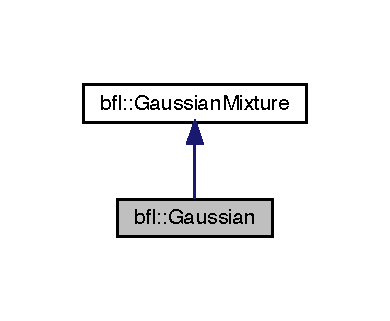
\includegraphics[width=187pt]{classbfl_1_1Gaussian__inherit__graph}
\end{center}
\end{figure}
\subsection*{Public Member Functions}
\begin{DoxyCompactItemize}
\item 
\mbox{\hyperlink{classbfl_1_1Gaussian_aa201bf4a8fe1192c9a701e9537691426}{Gaussian}} ()
\item 
\mbox{\hyperlink{classbfl_1_1Gaussian_aa096285a5065804c2f0838135de47875}{Gaussian}} (const std\+::size\+\_\+t \mbox{\hyperlink{classbfl_1_1GaussianMixture_a22a0fbc77f90d9d75e89d7898484c05a}{dim\+\_\+linear}})
\item 
\mbox{\hyperlink{classbfl_1_1Gaussian_a99507926f6b8df85b6a512c21afe2b50}{Gaussian}} (const std\+::size\+\_\+t \mbox{\hyperlink{classbfl_1_1GaussianMixture_a22a0fbc77f90d9d75e89d7898484c05a}{dim\+\_\+linear}}, const std\+::size\+\_\+t \mbox{\hyperlink{classbfl_1_1GaussianMixture_a23f3b92753266475a9bff8ee7e1c9518}{dim\+\_\+circular}})
\item 
Eigen\+::\+Ref$<$ Eigen\+::\+Vector\+Xd $>$ \mbox{\hyperlink{classbfl_1_1Gaussian_a31c06392bcbcc31d576e148001b681a0}{mean}} ()
\begin{DoxyCompactList}\small\item\em Non-\/virtual methods of \mbox{\hyperlink{classbfl_1_1GaussianMixture}{Gaussian\+Mixture}} are overriden here since a \mbox{\hyperlink{classbfl_1_1Gaussian}{Gaussian}} is a 1-\/component \mbox{\hyperlink{classbfl_1_1GaussianMixture}{Gaussian\+Mixture}}. \end{DoxyCompactList}\item 
const Eigen\+::\+Ref$<$ const Eigen\+::\+Vector\+Xd $>$ \mbox{\hyperlink{classbfl_1_1Gaussian_a1b9b1727e467cc671cbf5487c00c9b20}{mean}} () const
\item 
double \& \mbox{\hyperlink{classbfl_1_1Gaussian_aa19856ef77d8d6599ff22884174eda9a}{mean}} (const std\+::size\+\_\+t i)
\item 
const double \& \mbox{\hyperlink{classbfl_1_1Gaussian_a025d3985d2390300f2b999b71f1a2e3c}{mean}} (const std\+::size\+\_\+t i) const
\item 
Eigen\+::\+Ref$<$ Eigen\+::\+Matrix\+Xd $>$ \mbox{\hyperlink{classbfl_1_1Gaussian_a23dbc924dadc0061c392a7435eb3befe}{covariance}} ()
\item 
const Eigen\+::\+Ref$<$ const Eigen\+::\+Matrix\+Xd $>$ \mbox{\hyperlink{classbfl_1_1Gaussian_a696a82cf8c335970e5280010f5b8bc9f}{covariance}} () const
\item 
double \& \mbox{\hyperlink{classbfl_1_1Gaussian_ac24bc21ce7fbcf4999e88c1957697bd6}{covariance}} (const std\+::size\+\_\+t i, const std\+::size\+\_\+t j)
\item 
const double \& \mbox{\hyperlink{classbfl_1_1Gaussian_af0b2eb137164512658abfeb39d8337ed}{covariance}} (const std\+::size\+\_\+t i, const std\+::size\+\_\+t j) const
\item 
double \& \mbox{\hyperlink{classbfl_1_1Gaussian_aac053b84b9cf54506236bb38a9be7baa}{weight}} ()
\item 
const double \& \mbox{\hyperlink{classbfl_1_1Gaussian_a84a8482a20306e29b508a7235c01f2a6}{weight}} () const
\item 
virtual \mbox{\hyperlink{classbfl_1_1Gaussian_a073652fe6f52bf1833cdb3d73bec792f}{$\sim$\+Gaussian}} () noexcept
\item 
double \& \mbox{\hyperlink{classbfl_1_1GaussianMixture_a21013d54d99ca5bfd1ec566a0815821e}{mean}} (const std\+::size\+\_\+t i, const std\+::size\+\_\+t j)
\item 
const double \& \mbox{\hyperlink{classbfl_1_1GaussianMixture_ac3baa237bc22f156f57d4c02deb4f518}{mean}} (const std\+::size\+\_\+t i, const std\+::size\+\_\+t j) const
\item 
Eigen\+::\+Ref$<$ Eigen\+::\+Matrix\+Xd $>$ \mbox{\hyperlink{classbfl_1_1GaussianMixture_a80a6fa7d9edfc95103236378b4da3f7f}{covariance}} (const std\+::size\+\_\+t i)
\item 
double \& \mbox{\hyperlink{classbfl_1_1GaussianMixture_ad2c74407e682e3b4322df2d0e1cef28e}{covariance}} (const std\+::size\+\_\+t i, const std\+::size\+\_\+t j, const std\+::size\+\_\+t k)
\item 
const Eigen\+::\+Ref$<$ const Eigen\+::\+Matrix\+Xd $>$ \mbox{\hyperlink{classbfl_1_1GaussianMixture_a3cff0f507ed950fe6a5e0aba1bf8467a}{covariance}} (const std\+::size\+\_\+t i) const
\item 
const double \& \mbox{\hyperlink{classbfl_1_1GaussianMixture_a4ca0b098be0fc923f454e73e9dccf78f}{covariance}} (const std\+::size\+\_\+t i, const std\+::size\+\_\+t j, const std\+::size\+\_\+t k) const
\item 
double \& \mbox{\hyperlink{classbfl_1_1GaussianMixture_a44885fb208e33f37015d47f55d02ef50}{weight}} (const std\+::size\+\_\+t i)
\item 
const double \& \mbox{\hyperlink{classbfl_1_1GaussianMixture_a42672f88d9126f018715a4d258a57731}{weight}} (const std\+::size\+\_\+t i) const
\item 
bool \mbox{\hyperlink{classbfl_1_1GaussianMixture_aec4e807341e18c18faed041c41121cb7}{augment\+With\+Noise}} (const Eigen\+::\+Ref$<$ const Eigen\+::\+Matrix\+Xd $>$ \&noise\+\_\+covariance\+\_\+matrix)
\end{DoxyCompactItemize}
\subsection*{Public Attributes}
\begin{DoxyCompactItemize}
\item 
std\+::size\+\_\+t \mbox{\hyperlink{classbfl_1_1GaussianMixture_a02cc284327dbaa6b90c653dd2faccf88}{components}}
\item 
std\+::size\+\_\+t \mbox{\hyperlink{classbfl_1_1GaussianMixture_a3f2b18801e72fa3bf0d6edc778662a8d}{dim}}
\item 
std\+::size\+\_\+t \mbox{\hyperlink{classbfl_1_1GaussianMixture_a22a0fbc77f90d9d75e89d7898484c05a}{dim\+\_\+linear}}
\item 
std\+::size\+\_\+t \mbox{\hyperlink{classbfl_1_1GaussianMixture_a23f3b92753266475a9bff8ee7e1c9518}{dim\+\_\+circular}}
\item 
std\+::size\+\_\+t \mbox{\hyperlink{classbfl_1_1GaussianMixture_adaa8d9c6d03be835769cc848aba81067}{dim\+\_\+noise}}
\end{DoxyCompactItemize}
\subsection*{Protected Attributes}
\begin{DoxyCompactItemize}
\item 
Eigen\+::\+Matrix\+Xd \mbox{\hyperlink{classbfl_1_1GaussianMixture_a12a1175e838a753129f4cc133b2c1a9c}{mean\+\_\+}}
\item 
Eigen\+::\+Matrix\+Xd \mbox{\hyperlink{classbfl_1_1GaussianMixture_aab086cc1a89a8b7efd15303853e52920}{covariance\+\_\+}}
\item 
Eigen\+::\+Vector\+Xd \mbox{\hyperlink{classbfl_1_1GaussianMixture_ac9ce000575d6b29ad8e1a756d750faff}{weight\+\_\+}}
\end{DoxyCompactItemize}


\subsection{Detailed Description}


Definition at line 15 of file Gaussian.\+h.



\subsection{Constructor \& Destructor Documentation}
\mbox{\Hypertarget{classbfl_1_1Gaussian_aa201bf4a8fe1192c9a701e9537691426}\label{classbfl_1_1Gaussian_aa201bf4a8fe1192c9a701e9537691426}} 
\index{bfl\+::\+Gaussian@{bfl\+::\+Gaussian}!Gaussian@{Gaussian}}
\index{Gaussian@{Gaussian}!bfl\+::\+Gaussian@{bfl\+::\+Gaussian}}
\subsubsection{\texorpdfstring{Gaussian()}{Gaussian()}\hspace{0.1cm}{\footnotesize\ttfamily [1/3]}}
{\footnotesize\ttfamily Gaussian\+::\+Gaussian (\begin{DoxyParamCaption}{ }\end{DoxyParamCaption})}



Definition at line 8 of file Gaussian.\+cpp.

\mbox{\Hypertarget{classbfl_1_1Gaussian_aa096285a5065804c2f0838135de47875}\label{classbfl_1_1Gaussian_aa096285a5065804c2f0838135de47875}} 
\index{bfl\+::\+Gaussian@{bfl\+::\+Gaussian}!Gaussian@{Gaussian}}
\index{Gaussian@{Gaussian}!bfl\+::\+Gaussian@{bfl\+::\+Gaussian}}
\subsubsection{\texorpdfstring{Gaussian()}{Gaussian()}\hspace{0.1cm}{\footnotesize\ttfamily [2/3]}}
{\footnotesize\ttfamily Gaussian\+::\+Gaussian (\begin{DoxyParamCaption}\item[{const std\+::size\+\_\+t}]{dim\+\_\+linear }\end{DoxyParamCaption})}



Definition at line 11 of file Gaussian.\+cpp.

\mbox{\Hypertarget{classbfl_1_1Gaussian_a99507926f6b8df85b6a512c21afe2b50}\label{classbfl_1_1Gaussian_a99507926f6b8df85b6a512c21afe2b50}} 
\index{bfl\+::\+Gaussian@{bfl\+::\+Gaussian}!Gaussian@{Gaussian}}
\index{Gaussian@{Gaussian}!bfl\+::\+Gaussian@{bfl\+::\+Gaussian}}
\subsubsection{\texorpdfstring{Gaussian()}{Gaussian()}\hspace{0.1cm}{\footnotesize\ttfamily [3/3]}}
{\footnotesize\ttfamily Gaussian\+::\+Gaussian (\begin{DoxyParamCaption}\item[{const std\+::size\+\_\+t}]{dim\+\_\+linear,  }\item[{const std\+::size\+\_\+t}]{dim\+\_\+circular }\end{DoxyParamCaption})}



Definition at line 15 of file Gaussian.\+cpp.

\mbox{\Hypertarget{classbfl_1_1Gaussian_a073652fe6f52bf1833cdb3d73bec792f}\label{classbfl_1_1Gaussian_a073652fe6f52bf1833cdb3d73bec792f}} 
\index{bfl\+::\+Gaussian@{bfl\+::\+Gaussian}!````~Gaussian@{$\sim$\+Gaussian}}
\index{````~Gaussian@{$\sim$\+Gaussian}!bfl\+::\+Gaussian@{bfl\+::\+Gaussian}}
\subsubsection{\texorpdfstring{$\sim$\+Gaussian()}{~Gaussian()}}
{\footnotesize\ttfamily virtual bfl\+::\+Gaussian\+::$\sim$\+Gaussian (\begin{DoxyParamCaption}{ }\end{DoxyParamCaption})\hspace{0.3cm}{\ttfamily [inline]}, {\ttfamily [virtual]}, {\ttfamily [noexcept]}}



Definition at line 51 of file Gaussian.\+h.



\subsection{Member Function Documentation}
\mbox{\Hypertarget{classbfl_1_1GaussianMixture_aec4e807341e18c18faed041c41121cb7}\label{classbfl_1_1GaussianMixture_aec4e807341e18c18faed041c41121cb7}} 
\index{bfl\+::\+Gaussian@{bfl\+::\+Gaussian}!augment\+With\+Noise@{augment\+With\+Noise}}
\index{augment\+With\+Noise@{augment\+With\+Noise}!bfl\+::\+Gaussian@{bfl\+::\+Gaussian}}
\subsubsection{\texorpdfstring{augment\+With\+Noise()}{augmentWithNoise()}}
{\footnotesize\ttfamily bool Gaussian\+Mixture\+::augment\+With\+Noise (\begin{DoxyParamCaption}\item[{const Eigen\+::\+Ref$<$ const Eigen\+::\+Matrix\+Xd $>$ \&}]{noise\+\_\+covariance\+\_\+matrix }\end{DoxyParamCaption})\hspace{0.3cm}{\ttfamily [inherited]}}



Definition at line 136 of file Gaussian\+Mixture.\+cpp.



References bfl\+::\+Gaussian\+Mixture\+::components, bfl\+::\+Gaussian\+Mixture\+::covariance\+\_\+, bfl\+::\+Gaussian\+Mixture\+::dim, bfl\+::\+Gaussian\+Mixture\+::dim\+\_\+circular, bfl\+::\+Gaussian\+Mixture\+::dim\+\_\+linear, bfl\+::\+Gaussian\+Mixture\+::dim\+\_\+noise, and bfl\+::\+Gaussian\+Mixture\+::mean\+\_\+.



Referenced by bfl\+::\+U\+K\+F\+Correction\+::correct\+Step(), and bfl\+::\+U\+K\+F\+Prediction\+::predict\+Step().

\mbox{\Hypertarget{classbfl_1_1GaussianMixture_a80a6fa7d9edfc95103236378b4da3f7f}\label{classbfl_1_1GaussianMixture_a80a6fa7d9edfc95103236378b4da3f7f}} 
\index{bfl\+::\+Gaussian@{bfl\+::\+Gaussian}!covariance@{covariance}}
\index{covariance@{covariance}!bfl\+::\+Gaussian@{bfl\+::\+Gaussian}}
\subsubsection{\texorpdfstring{covariance()}{covariance()}\hspace{0.1cm}{\footnotesize\ttfamily [1/8]}}
{\footnotesize\ttfamily Ref$<$ Matrix\+Xd $>$ Gaussian\+Mixture\+::covariance (\begin{DoxyParamCaption}\item[{const std\+::size\+\_\+t}]{i }\end{DoxyParamCaption})\hspace{0.3cm}{\ttfamily [inherited]}}



Definition at line 82 of file Gaussian\+Mixture.\+cpp.



References bfl\+::\+Gaussian\+Mixture\+::covariance\+\_\+, and bfl\+::\+Gaussian\+Mixture\+::dim.

\mbox{\Hypertarget{classbfl_1_1Gaussian_a23dbc924dadc0061c392a7435eb3befe}\label{classbfl_1_1Gaussian_a23dbc924dadc0061c392a7435eb3befe}} 
\index{bfl\+::\+Gaussian@{bfl\+::\+Gaussian}!covariance@{covariance}}
\index{covariance@{covariance}!bfl\+::\+Gaussian@{bfl\+::\+Gaussian}}
\subsubsection{\texorpdfstring{covariance()}{covariance()}\hspace{0.1cm}{\footnotesize\ttfamily [2/8]}}
{\footnotesize\ttfamily Ref$<$ Matrix\+Xd $>$ Gaussian\+::covariance (\begin{DoxyParamCaption}{ }\end{DoxyParamCaption})}



Definition at line 43 of file Gaussian.\+cpp.



References bfl\+::\+Gaussian\+Mixture\+::covariance\+\_\+.

\mbox{\Hypertarget{classbfl_1_1GaussianMixture_ad2c74407e682e3b4322df2d0e1cef28e}\label{classbfl_1_1GaussianMixture_ad2c74407e682e3b4322df2d0e1cef28e}} 
\index{bfl\+::\+Gaussian@{bfl\+::\+Gaussian}!covariance@{covariance}}
\index{covariance@{covariance}!bfl\+::\+Gaussian@{bfl\+::\+Gaussian}}
\subsubsection{\texorpdfstring{covariance()}{covariance()}\hspace{0.1cm}{\footnotesize\ttfamily [3/8]}}
{\footnotesize\ttfamily double \& Gaussian\+Mixture\+::covariance (\begin{DoxyParamCaption}\item[{const std\+::size\+\_\+t}]{i,  }\item[{const std\+::size\+\_\+t}]{j,  }\item[{const std\+::size\+\_\+t}]{k }\end{DoxyParamCaption})\hspace{0.3cm}{\ttfamily [inherited]}}



Definition at line 88 of file Gaussian\+Mixture.\+cpp.



References bfl\+::\+Gaussian\+Mixture\+::covariance\+\_\+, and bfl\+::\+Gaussian\+Mixture\+::dim.

\mbox{\Hypertarget{classbfl_1_1Gaussian_a696a82cf8c335970e5280010f5b8bc9f}\label{classbfl_1_1Gaussian_a696a82cf8c335970e5280010f5b8bc9f}} 
\index{bfl\+::\+Gaussian@{bfl\+::\+Gaussian}!covariance@{covariance}}
\index{covariance@{covariance}!bfl\+::\+Gaussian@{bfl\+::\+Gaussian}}
\subsubsection{\texorpdfstring{covariance()}{covariance()}\hspace{0.1cm}{\footnotesize\ttfamily [4/8]}}
{\footnotesize\ttfamily const Ref$<$ const Matrix\+Xd $>$ Gaussian\+::covariance (\begin{DoxyParamCaption}{ }\end{DoxyParamCaption}) const}



Definition at line 49 of file Gaussian.\+cpp.



References bfl\+::\+Gaussian\+Mixture\+::covariance\+\_\+.

\mbox{\Hypertarget{classbfl_1_1Gaussian_ac24bc21ce7fbcf4999e88c1957697bd6}\label{classbfl_1_1Gaussian_ac24bc21ce7fbcf4999e88c1957697bd6}} 
\index{bfl\+::\+Gaussian@{bfl\+::\+Gaussian}!covariance@{covariance}}
\index{covariance@{covariance}!bfl\+::\+Gaussian@{bfl\+::\+Gaussian}}
\subsubsection{\texorpdfstring{covariance()}{covariance()}\hspace{0.1cm}{\footnotesize\ttfamily [5/8]}}
{\footnotesize\ttfamily double \& Gaussian\+::covariance (\begin{DoxyParamCaption}\item[{const std\+::size\+\_\+t}]{i,  }\item[{const std\+::size\+\_\+t}]{j }\end{DoxyParamCaption})}



Definition at line 55 of file Gaussian.\+cpp.



References bfl\+::\+Gaussian\+Mixture\+::covariance\+\_\+.

\mbox{\Hypertarget{classbfl_1_1GaussianMixture_a3cff0f507ed950fe6a5e0aba1bf8467a}\label{classbfl_1_1GaussianMixture_a3cff0f507ed950fe6a5e0aba1bf8467a}} 
\index{bfl\+::\+Gaussian@{bfl\+::\+Gaussian}!covariance@{covariance}}
\index{covariance@{covariance}!bfl\+::\+Gaussian@{bfl\+::\+Gaussian}}
\subsubsection{\texorpdfstring{covariance()}{covariance()}\hspace{0.1cm}{\footnotesize\ttfamily [6/8]}}
{\footnotesize\ttfamily const Ref$<$ const Matrix\+Xd $>$ Gaussian\+Mixture\+::covariance (\begin{DoxyParamCaption}\item[{const std\+::size\+\_\+t}]{i }\end{DoxyParamCaption}) const\hspace{0.3cm}{\ttfamily [inherited]}}



Definition at line 100 of file Gaussian\+Mixture.\+cpp.



References bfl\+::\+Gaussian\+Mixture\+::covariance\+\_\+, and bfl\+::\+Gaussian\+Mixture\+::dim.

\mbox{\Hypertarget{classbfl_1_1Gaussian_af0b2eb137164512658abfeb39d8337ed}\label{classbfl_1_1Gaussian_af0b2eb137164512658abfeb39d8337ed}} 
\index{bfl\+::\+Gaussian@{bfl\+::\+Gaussian}!covariance@{covariance}}
\index{covariance@{covariance}!bfl\+::\+Gaussian@{bfl\+::\+Gaussian}}
\subsubsection{\texorpdfstring{covariance()}{covariance()}\hspace{0.1cm}{\footnotesize\ttfamily [7/8]}}
{\footnotesize\ttfamily const double \& Gaussian\+::covariance (\begin{DoxyParamCaption}\item[{const std\+::size\+\_\+t}]{i,  }\item[{const std\+::size\+\_\+t}]{j }\end{DoxyParamCaption}) const}



Definition at line 62 of file Gaussian.\+cpp.



References bfl\+::\+Gaussian\+Mixture\+::covariance\+\_\+.

\mbox{\Hypertarget{classbfl_1_1GaussianMixture_a4ca0b098be0fc923f454e73e9dccf78f}\label{classbfl_1_1GaussianMixture_a4ca0b098be0fc923f454e73e9dccf78f}} 
\index{bfl\+::\+Gaussian@{bfl\+::\+Gaussian}!covariance@{covariance}}
\index{covariance@{covariance}!bfl\+::\+Gaussian@{bfl\+::\+Gaussian}}
\subsubsection{\texorpdfstring{covariance()}{covariance()}\hspace{0.1cm}{\footnotesize\ttfamily [8/8]}}
{\footnotesize\ttfamily const double \& Gaussian\+Mixture\+::covariance (\begin{DoxyParamCaption}\item[{const std\+::size\+\_\+t}]{i,  }\item[{const std\+::size\+\_\+t}]{j,  }\item[{const std\+::size\+\_\+t}]{k }\end{DoxyParamCaption}) const\hspace{0.3cm}{\ttfamily [inherited]}}



Definition at line 106 of file Gaussian\+Mixture.\+cpp.



References bfl\+::\+Gaussian\+Mixture\+::covariance\+\_\+, and bfl\+::\+Gaussian\+Mixture\+::dim.

\mbox{\Hypertarget{classbfl_1_1GaussianMixture_a21013d54d99ca5bfd1ec566a0815821e}\label{classbfl_1_1GaussianMixture_a21013d54d99ca5bfd1ec566a0815821e}} 
\index{bfl\+::\+Gaussian@{bfl\+::\+Gaussian}!mean@{mean}}
\index{mean@{mean}!bfl\+::\+Gaussian@{bfl\+::\+Gaussian}}
\subsubsection{\texorpdfstring{mean()}{mean()}\hspace{0.1cm}{\footnotesize\ttfamily [1/6]}}
{\footnotesize\ttfamily double \& Gaussian\+Mixture\+::mean (\begin{DoxyParamCaption}\item[{const std\+::size\+\_\+t}]{i,  }\item[{const std\+::size\+\_\+t}]{j }\end{DoxyParamCaption})\hspace{0.3cm}{\ttfamily [inherited]}}



Definition at line 52 of file Gaussian\+Mixture.\+cpp.



References bfl\+::\+Gaussian\+Mixture\+::mean\+\_\+.

\mbox{\Hypertarget{classbfl_1_1Gaussian_a31c06392bcbcc31d576e148001b681a0}\label{classbfl_1_1Gaussian_a31c06392bcbcc31d576e148001b681a0}} 
\index{bfl\+::\+Gaussian@{bfl\+::\+Gaussian}!mean@{mean}}
\index{mean@{mean}!bfl\+::\+Gaussian@{bfl\+::\+Gaussian}}
\subsubsection{\texorpdfstring{mean()}{mean()}\hspace{0.1cm}{\footnotesize\ttfamily [2/6]}}
{\footnotesize\ttfamily Ref$<$ Vector\+Xd $>$ Gaussian\+::mean (\begin{DoxyParamCaption}{ }\end{DoxyParamCaption})}



Non-\/virtual methods of \mbox{\hyperlink{classbfl_1_1GaussianMixture}{Gaussian\+Mixture}} are overriden here since a \mbox{\hyperlink{classbfl_1_1Gaussian}{Gaussian}} is a 1-\/component \mbox{\hyperlink{classbfl_1_1GaussianMixture}{Gaussian\+Mixture}}. 

Hence it is better to return a Ref$<$\+Vector\+Xd$>$ as the mean, rather than a Ref$<$\+Matrix\+Xd$>$, and a double\& as the weight, rather than a Ref$<$\+Vector\+Xd$>$\&. 

Definition at line 19 of file Gaussian.\+cpp.



References bfl\+::\+Gaussian\+Mixture\+::mean\+\_\+.

\mbox{\Hypertarget{classbfl_1_1Gaussian_a1b9b1727e467cc671cbf5487c00c9b20}\label{classbfl_1_1Gaussian_a1b9b1727e467cc671cbf5487c00c9b20}} 
\index{bfl\+::\+Gaussian@{bfl\+::\+Gaussian}!mean@{mean}}
\index{mean@{mean}!bfl\+::\+Gaussian@{bfl\+::\+Gaussian}}
\subsubsection{\texorpdfstring{mean()}{mean()}\hspace{0.1cm}{\footnotesize\ttfamily [3/6]}}
{\footnotesize\ttfamily const Ref$<$ const Vector\+Xd $>$ Gaussian\+::mean (\begin{DoxyParamCaption}{ }\end{DoxyParamCaption}) const}



Definition at line 25 of file Gaussian.\+cpp.



References bfl\+::\+Gaussian\+Mixture\+::mean\+\_\+.

\mbox{\Hypertarget{classbfl_1_1GaussianMixture_ac3baa237bc22f156f57d4c02deb4f518}\label{classbfl_1_1GaussianMixture_ac3baa237bc22f156f57d4c02deb4f518}} 
\index{bfl\+::\+Gaussian@{bfl\+::\+Gaussian}!mean@{mean}}
\index{mean@{mean}!bfl\+::\+Gaussian@{bfl\+::\+Gaussian}}
\subsubsection{\texorpdfstring{mean()}{mean()}\hspace{0.1cm}{\footnotesize\ttfamily [4/6]}}
{\footnotesize\ttfamily const double \& Gaussian\+Mixture\+::mean (\begin{DoxyParamCaption}\item[{const std\+::size\+\_\+t}]{i,  }\item[{const std\+::size\+\_\+t}]{j }\end{DoxyParamCaption}) const\hspace{0.3cm}{\ttfamily [inherited]}}



Definition at line 70 of file Gaussian\+Mixture.\+cpp.



References bfl\+::\+Gaussian\+Mixture\+::mean\+\_\+.

\mbox{\Hypertarget{classbfl_1_1Gaussian_aa19856ef77d8d6599ff22884174eda9a}\label{classbfl_1_1Gaussian_aa19856ef77d8d6599ff22884174eda9a}} 
\index{bfl\+::\+Gaussian@{bfl\+::\+Gaussian}!mean@{mean}}
\index{mean@{mean}!bfl\+::\+Gaussian@{bfl\+::\+Gaussian}}
\subsubsection{\texorpdfstring{mean()}{mean()}\hspace{0.1cm}{\footnotesize\ttfamily [5/6]}}
{\footnotesize\ttfamily double \& Gaussian\+::mean (\begin{DoxyParamCaption}\item[{const std\+::size\+\_\+t}]{i }\end{DoxyParamCaption})}



Definition at line 31 of file Gaussian.\+cpp.



References bfl\+::\+Gaussian\+Mixture\+::mean\+\_\+.

\mbox{\Hypertarget{classbfl_1_1Gaussian_a025d3985d2390300f2b999b71f1a2e3c}\label{classbfl_1_1Gaussian_a025d3985d2390300f2b999b71f1a2e3c}} 
\index{bfl\+::\+Gaussian@{bfl\+::\+Gaussian}!mean@{mean}}
\index{mean@{mean}!bfl\+::\+Gaussian@{bfl\+::\+Gaussian}}
\subsubsection{\texorpdfstring{mean()}{mean()}\hspace{0.1cm}{\footnotesize\ttfamily [6/6]}}
{\footnotesize\ttfamily const double \& Gaussian\+::mean (\begin{DoxyParamCaption}\item[{const std\+::size\+\_\+t}]{i }\end{DoxyParamCaption}) const}



Definition at line 37 of file Gaussian.\+cpp.



References bfl\+::\+Gaussian\+Mixture\+::mean\+\_\+.

\mbox{\Hypertarget{classbfl_1_1Gaussian_aac053b84b9cf54506236bb38a9be7baa}\label{classbfl_1_1Gaussian_aac053b84b9cf54506236bb38a9be7baa}} 
\index{bfl\+::\+Gaussian@{bfl\+::\+Gaussian}!weight@{weight}}
\index{weight@{weight}!bfl\+::\+Gaussian@{bfl\+::\+Gaussian}}
\subsubsection{\texorpdfstring{weight()}{weight()}\hspace{0.1cm}{\footnotesize\ttfamily [1/4]}}
{\footnotesize\ttfamily double \& Gaussian\+::weight (\begin{DoxyParamCaption}{ }\end{DoxyParamCaption})}



Definition at line 68 of file Gaussian.\+cpp.



References bfl\+::\+Gaussian\+Mixture\+::weight\+\_\+.

\mbox{\Hypertarget{classbfl_1_1Gaussian_a84a8482a20306e29b508a7235c01f2a6}\label{classbfl_1_1Gaussian_a84a8482a20306e29b508a7235c01f2a6}} 
\index{bfl\+::\+Gaussian@{bfl\+::\+Gaussian}!weight@{weight}}
\index{weight@{weight}!bfl\+::\+Gaussian@{bfl\+::\+Gaussian}}
\subsubsection{\texorpdfstring{weight()}{weight()}\hspace{0.1cm}{\footnotesize\ttfamily [2/4]}}
{\footnotesize\ttfamily const double \& Gaussian\+::weight (\begin{DoxyParamCaption}{ }\end{DoxyParamCaption}) const}



Definition at line 74 of file Gaussian.\+cpp.



References bfl\+::\+Gaussian\+Mixture\+::weight\+\_\+.

\mbox{\Hypertarget{classbfl_1_1GaussianMixture_a44885fb208e33f37015d47f55d02ef50}\label{classbfl_1_1GaussianMixture_a44885fb208e33f37015d47f55d02ef50}} 
\index{bfl\+::\+Gaussian@{bfl\+::\+Gaussian}!weight@{weight}}
\index{weight@{weight}!bfl\+::\+Gaussian@{bfl\+::\+Gaussian}}
\subsubsection{\texorpdfstring{weight()}{weight()}\hspace{0.1cm}{\footnotesize\ttfamily [3/4]}}
{\footnotesize\ttfamily double \& Gaussian\+Mixture\+::weight (\begin{DoxyParamCaption}\item[{const std\+::size\+\_\+t}]{i }\end{DoxyParamCaption})\hspace{0.3cm}{\ttfamily [inherited]}}



Definition at line 118 of file Gaussian\+Mixture.\+cpp.



References bfl\+::\+Gaussian\+Mixture\+::weight\+\_\+.

\mbox{\Hypertarget{classbfl_1_1GaussianMixture_a42672f88d9126f018715a4d258a57731}\label{classbfl_1_1GaussianMixture_a42672f88d9126f018715a4d258a57731}} 
\index{bfl\+::\+Gaussian@{bfl\+::\+Gaussian}!weight@{weight}}
\index{weight@{weight}!bfl\+::\+Gaussian@{bfl\+::\+Gaussian}}
\subsubsection{\texorpdfstring{weight()}{weight()}\hspace{0.1cm}{\footnotesize\ttfamily [4/4]}}
{\footnotesize\ttfamily const double \& Gaussian\+Mixture\+::weight (\begin{DoxyParamCaption}\item[{const std\+::size\+\_\+t}]{i }\end{DoxyParamCaption}) const\hspace{0.3cm}{\ttfamily [inherited]}}



Definition at line 130 of file Gaussian\+Mixture.\+cpp.



References bfl\+::\+Gaussian\+Mixture\+::weight\+\_\+.



\subsection{Member Data Documentation}
\mbox{\Hypertarget{classbfl_1_1GaussianMixture_a02cc284327dbaa6b90c653dd2faccf88}\label{classbfl_1_1GaussianMixture_a02cc284327dbaa6b90c653dd2faccf88}} 
\index{bfl\+::\+Gaussian@{bfl\+::\+Gaussian}!components@{components}}
\index{components@{components}!bfl\+::\+Gaussian@{bfl\+::\+Gaussian}}
\subsubsection{\texorpdfstring{components}{components}}
{\footnotesize\ttfamily std\+::size\+\_\+t bfl\+::\+Gaussian\+Mixture\+::components\hspace{0.3cm}{\ttfamily [inherited]}}



Definition at line 58 of file Gaussian\+Mixture.\+h.



Referenced by bfl\+::\+Gaussian\+Mixture\+::augment\+With\+Noise(), bfl\+::\+K\+F\+Correction\+::correct\+Step(), bfl\+::\+U\+K\+F\+Correction\+::correct\+Step(), bfl\+::\+G\+P\+F\+Correction\+::correct\+Step(), bfl\+::\+S\+U\+K\+F\+Correction\+::correct\+Step(), bfl\+::\+Particle\+Set\+::operator+=(), bfl\+::\+K\+F\+Prediction\+::predict\+Step(), bfl\+::sigma\+\_\+point\+::sigma\+\_\+point(), and bfl\+::sigma\+\_\+point\+::unscented\+\_\+transform().

\mbox{\Hypertarget{classbfl_1_1GaussianMixture_aab086cc1a89a8b7efd15303853e52920}\label{classbfl_1_1GaussianMixture_aab086cc1a89a8b7efd15303853e52920}} 
\index{bfl\+::\+Gaussian@{bfl\+::\+Gaussian}!covariance\+\_\+@{covariance\+\_\+}}
\index{covariance\+\_\+@{covariance\+\_\+}!bfl\+::\+Gaussian@{bfl\+::\+Gaussian}}
\subsubsection{\texorpdfstring{covariance\+\_\+}{covariance\_}}
{\footnotesize\ttfamily Eigen\+::\+Matrix\+Xd bfl\+::\+Gaussian\+Mixture\+::covariance\+\_\+\hspace{0.3cm}{\ttfamily [protected]}, {\ttfamily [inherited]}}



Definition at line 71 of file Gaussian\+Mixture.\+h.



Referenced by bfl\+::\+Gaussian\+Mixture\+::augment\+With\+Noise(), bfl\+::\+Gaussian\+Mixture\+::covariance(), covariance(), and bfl\+::\+Particle\+Set\+::operator+=().

\mbox{\Hypertarget{classbfl_1_1GaussianMixture_a3f2b18801e72fa3bf0d6edc778662a8d}\label{classbfl_1_1GaussianMixture_a3f2b18801e72fa3bf0d6edc778662a8d}} 
\index{bfl\+::\+Gaussian@{bfl\+::\+Gaussian}!dim@{dim}}
\index{dim@{dim}!bfl\+::\+Gaussian@{bfl\+::\+Gaussian}}
\subsubsection{\texorpdfstring{dim}{dim}}
{\footnotesize\ttfamily std\+::size\+\_\+t bfl\+::\+Gaussian\+Mixture\+::dim\hspace{0.3cm}{\ttfamily [inherited]}}



Definition at line 60 of file Gaussian\+Mixture.\+h.



Referenced by bfl\+::\+Gaussian\+Mixture\+::augment\+With\+Noise(), bfl\+::\+S\+U\+K\+F\+Correction\+::correct\+Step(), bfl\+::\+Gaussian\+Mixture\+::covariance(), bfl\+::sigma\+\_\+point\+::sigma\+\_\+point(), and bfl\+::sigma\+\_\+point\+::unscented\+\_\+transform().

\mbox{\Hypertarget{classbfl_1_1GaussianMixture_a23f3b92753266475a9bff8ee7e1c9518}\label{classbfl_1_1GaussianMixture_a23f3b92753266475a9bff8ee7e1c9518}} 
\index{bfl\+::\+Gaussian@{bfl\+::\+Gaussian}!dim\+\_\+circular@{dim\+\_\+circular}}
\index{dim\+\_\+circular@{dim\+\_\+circular}!bfl\+::\+Gaussian@{bfl\+::\+Gaussian}}
\subsubsection{\texorpdfstring{dim\+\_\+circular}{dim\_circular}}
{\footnotesize\ttfamily std\+::size\+\_\+t bfl\+::\+Gaussian\+Mixture\+::dim\+\_\+circular\hspace{0.3cm}{\ttfamily [inherited]}}



Definition at line 64 of file Gaussian\+Mixture.\+h.



Referenced by bfl\+::\+Gaussian\+Mixture\+::augment\+With\+Noise(), bfl\+::\+S\+U\+K\+F\+Correction\+::correct\+Step(), bfl\+::\+Resampling\+With\+Prior\+::resample(), bfl\+::sigma\+\_\+point\+::sigma\+\_\+point(), and bfl\+::sigma\+\_\+point\+::unscented\+\_\+transform().

\mbox{\Hypertarget{classbfl_1_1GaussianMixture_a22a0fbc77f90d9d75e89d7898484c05a}\label{classbfl_1_1GaussianMixture_a22a0fbc77f90d9d75e89d7898484c05a}} 
\index{bfl\+::\+Gaussian@{bfl\+::\+Gaussian}!dim\+\_\+linear@{dim\+\_\+linear}}
\index{dim\+\_\+linear@{dim\+\_\+linear}!bfl\+::\+Gaussian@{bfl\+::\+Gaussian}}
\subsubsection{\texorpdfstring{dim\+\_\+linear}{dim\_linear}}
{\footnotesize\ttfamily std\+::size\+\_\+t bfl\+::\+Gaussian\+Mixture\+::dim\+\_\+linear\hspace{0.3cm}{\ttfamily [inherited]}}



Definition at line 62 of file Gaussian\+Mixture.\+h.



Referenced by bfl\+::\+Gaussian\+Mixture\+::augment\+With\+Noise(), bfl\+::\+S\+U\+K\+F\+Correction\+::correct\+Step(), bfl\+::\+Resampling\+With\+Prior\+::resample(), bfl\+::sigma\+\_\+point\+::sigma\+\_\+point(), and bfl\+::sigma\+\_\+point\+::unscented\+\_\+transform().

\mbox{\Hypertarget{classbfl_1_1GaussianMixture_adaa8d9c6d03be835769cc848aba81067}\label{classbfl_1_1GaussianMixture_adaa8d9c6d03be835769cc848aba81067}} 
\index{bfl\+::\+Gaussian@{bfl\+::\+Gaussian}!dim\+\_\+noise@{dim\+\_\+noise}}
\index{dim\+\_\+noise@{dim\+\_\+noise}!bfl\+::\+Gaussian@{bfl\+::\+Gaussian}}
\subsubsection{\texorpdfstring{dim\+\_\+noise}{dim\_noise}}
{\footnotesize\ttfamily std\+::size\+\_\+t bfl\+::\+Gaussian\+Mixture\+::dim\+\_\+noise\hspace{0.3cm}{\ttfamily [inherited]}}



Definition at line 66 of file Gaussian\+Mixture.\+h.



Referenced by bfl\+::\+Gaussian\+Mixture\+::augment\+With\+Noise(), and bfl\+::sigma\+\_\+point\+::sigma\+\_\+point().

\mbox{\Hypertarget{classbfl_1_1GaussianMixture_a12a1175e838a753129f4cc133b2c1a9c}\label{classbfl_1_1GaussianMixture_a12a1175e838a753129f4cc133b2c1a9c}} 
\index{bfl\+::\+Gaussian@{bfl\+::\+Gaussian}!mean\+\_\+@{mean\+\_\+}}
\index{mean\+\_\+@{mean\+\_\+}!bfl\+::\+Gaussian@{bfl\+::\+Gaussian}}
\subsubsection{\texorpdfstring{mean\+\_\+}{mean\_}}
{\footnotesize\ttfamily Eigen\+::\+Matrix\+Xd bfl\+::\+Gaussian\+Mixture\+::mean\+\_\+\hspace{0.3cm}{\ttfamily [protected]}, {\ttfamily [inherited]}}



Definition at line 69 of file Gaussian\+Mixture.\+h.



Referenced by bfl\+::\+Gaussian\+Mixture\+::augment\+With\+Noise(), bfl\+::\+Gaussian\+Mixture\+::mean(), mean(), and bfl\+::\+Particle\+Set\+::operator+=().

\mbox{\Hypertarget{classbfl_1_1GaussianMixture_ac9ce000575d6b29ad8e1a756d750faff}\label{classbfl_1_1GaussianMixture_ac9ce000575d6b29ad8e1a756d750faff}} 
\index{bfl\+::\+Gaussian@{bfl\+::\+Gaussian}!weight\+\_\+@{weight\+\_\+}}
\index{weight\+\_\+@{weight\+\_\+}!bfl\+::\+Gaussian@{bfl\+::\+Gaussian}}
\subsubsection{\texorpdfstring{weight\+\_\+}{weight\_}}
{\footnotesize\ttfamily Eigen\+::\+Vector\+Xd bfl\+::\+Gaussian\+Mixture\+::weight\+\_\+\hspace{0.3cm}{\ttfamily [protected]}, {\ttfamily [inherited]}}



Definition at line 73 of file Gaussian\+Mixture.\+h.



Referenced by bfl\+::\+Particle\+Set\+::operator+=(), weight(), and bfl\+::\+Gaussian\+Mixture\+::weight().



The documentation for this class was generated from the following files\+:\begin{DoxyCompactItemize}
\item 
/\+Users/\+Claudio/\+Git\+Hub/bayes-\/filters-\/lib/src/\+Bayes\+Filters/include/\+Bayes\+Filters/\mbox{\hyperlink{Gaussian_8h}{Gaussian.\+h}}\item 
/\+Users/\+Claudio/\+Git\+Hub/bayes-\/filters-\/lib/src/\+Bayes\+Filters/src/\mbox{\hyperlink{Gaussian_8cpp}{Gaussian.\+cpp}}\end{DoxyCompactItemize}

\hypertarget{classbfl_1_1GaussianCorrection}{}\section{bfl\+:\+:Gaussian\+Correction Class Reference}
\label{classbfl_1_1GaussianCorrection}\index{bfl\+::\+Gaussian\+Correction@{bfl\+::\+Gaussian\+Correction}}


{\ttfamily \#include $<$Gaussian\+Correction.\+h$>$}



Inheritance diagram for bfl\+:\+:Gaussian\+Correction\+:
\nopagebreak
\begin{figure}[H]
\begin{center}
\leavevmode
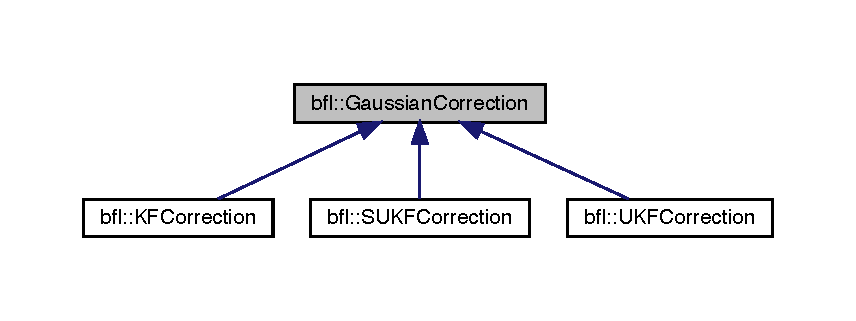
\includegraphics[width=350pt]{classbfl_1_1GaussianCorrection__inherit__graph}
\end{center}
\end{figure}
\subsection*{Public Member Functions}
\begin{DoxyCompactItemize}
\item 
virtual \mbox{\hyperlink{classbfl_1_1GaussianCorrection_a0144ae562cdda69763e8b6af2ed45669}{$\sim$\+Gaussian\+Correction}} () noexcept
\item 
void \mbox{\hyperlink{classbfl_1_1GaussianCorrection_a6308c8af37a1a451eba8e87e73952c84}{correct}} (const \mbox{\hyperlink{classbfl_1_1GaussianMixture}{Gaussian\+Mixture}} \&pred\+\_\+state, \mbox{\hyperlink{classbfl_1_1GaussianMixture}{Gaussian\+Mixture}} \&corr\+\_\+state)
\item 
bool \mbox{\hyperlink{classbfl_1_1GaussianCorrection_a986b05b149650ea4dd725b10700db57f}{skip}} (const bool status)
\item 
virtual std\+::pair$<$ bool, Eigen\+::\+Vector\+Xd $>$ \mbox{\hyperlink{classbfl_1_1GaussianCorrection_a955702adbdad6448d8f306752d3d0868}{get\+Likelihood}} ()
\end{DoxyCompactItemize}
\subsection*{Protected Member Functions}
\begin{DoxyCompactItemize}
\item 
virtual void \mbox{\hyperlink{classbfl_1_1GaussianCorrection_af30322d949e8135e1ec243bd6df00c18}{correct\+Step}} (const \mbox{\hyperlink{classbfl_1_1GaussianMixture}{Gaussian\+Mixture}} \&pred\+\_\+state, \mbox{\hyperlink{classbfl_1_1GaussianMixture}{Gaussian\+Mixture}} \&corr\+\_\+state)=0
\item 
virtual std\+::pair$<$ bool, Eigen\+::\+Vector\+Xd $>$ \mbox{\hyperlink{classbfl_1_1GaussianCorrection_a08e227b697ffbaf97c85fb4b17c99fd4}{likelihood}} (const Eigen\+::\+Ref$<$ const Eigen\+::\+Matrix\+Xd $>$ \&innovations)=0
\item 
virtual \mbox{\hyperlink{classbfl_1_1MeasurementModel}{Measurement\+Model}} \& \mbox{\hyperlink{classbfl_1_1GaussianCorrection_af609a22d84cc17a7337486c339ef30c3}{get\+Measurement\+Model}} ()=0
\item 
\mbox{\hyperlink{classbfl_1_1GaussianCorrection_a0ec06180aaf28ccaea798470a83b5f57}{Gaussian\+Correction}} () noexcept
\item 
\mbox{\hyperlink{classbfl_1_1GaussianCorrection_af901442309ecdc64607ab256aabc78a7}{Gaussian\+Correction}} (\mbox{\hyperlink{classbfl_1_1GaussianCorrection}{Gaussian\+Correction}} \&\&gaussian\+\_\+correction) noexcept
\end{DoxyCompactItemize}
\subsection*{Private Attributes}
\begin{DoxyCompactItemize}
\item 
bool \mbox{\hyperlink{classbfl_1_1GaussianCorrection_a6941174f7c3e3bb380e89bb6b4429f5e}{skip\+\_\+}} = false
\end{DoxyCompactItemize}
\subsection*{Friends}
\begin{DoxyCompactItemize}
\item 
class \mbox{\hyperlink{classbfl_1_1GaussianCorrection_a78bd8d7a082c77910c4ce95135781e2c}{Gaussian\+Correction\+Decorator}}
\item 
class \mbox{\hyperlink{classbfl_1_1GaussianCorrection_a5bc4f3f9c22a163bbcaac8d54f37a355}{G\+P\+F\+Correction}}
\end{DoxyCompactItemize}


\subsection{Detailed Description}


Definition at line 14 of file Gaussian\+Correction.\+h.



\subsection{Constructor \& Destructor Documentation}
\mbox{\Hypertarget{classbfl_1_1GaussianCorrection_a0144ae562cdda69763e8b6af2ed45669}\label{classbfl_1_1GaussianCorrection_a0144ae562cdda69763e8b6af2ed45669}} 
\index{bfl\+::\+Gaussian\+Correction@{bfl\+::\+Gaussian\+Correction}!````~Gaussian\+Correction@{$\sim$\+Gaussian\+Correction}}
\index{````~Gaussian\+Correction@{$\sim$\+Gaussian\+Correction}!bfl\+::\+Gaussian\+Correction@{bfl\+::\+Gaussian\+Correction}}
\subsubsection{\texorpdfstring{$\sim$\+Gaussian\+Correction()}{~GaussianCorrection()}}
{\footnotesize\ttfamily virtual bfl\+::\+Gaussian\+Correction\+::$\sim$\+Gaussian\+Correction (\begin{DoxyParamCaption}{ }\end{DoxyParamCaption})\hspace{0.3cm}{\ttfamily [inline]}, {\ttfamily [virtual]}, {\ttfamily [noexcept]}}



Definition at line 17 of file Gaussian\+Correction.\+h.

\mbox{\Hypertarget{classbfl_1_1GaussianCorrection_a0ec06180aaf28ccaea798470a83b5f57}\label{classbfl_1_1GaussianCorrection_a0ec06180aaf28ccaea798470a83b5f57}} 
\index{bfl\+::\+Gaussian\+Correction@{bfl\+::\+Gaussian\+Correction}!Gaussian\+Correction@{Gaussian\+Correction}}
\index{Gaussian\+Correction@{Gaussian\+Correction}!bfl\+::\+Gaussian\+Correction@{bfl\+::\+Gaussian\+Correction}}
\subsubsection{\texorpdfstring{Gaussian\+Correction()}{GaussianCorrection()}\hspace{0.1cm}{\footnotesize\ttfamily [1/2]}}
{\footnotesize\ttfamily Gaussian\+Correction\+::\+Gaussian\+Correction (\begin{DoxyParamCaption}{ }\end{DoxyParamCaption})\hspace{0.3cm}{\ttfamily [protected]}, {\ttfamily [noexcept]}}



Definition at line 7 of file Gaussian\+Correction.\+cpp.

\mbox{\Hypertarget{classbfl_1_1GaussianCorrection_af901442309ecdc64607ab256aabc78a7}\label{classbfl_1_1GaussianCorrection_af901442309ecdc64607ab256aabc78a7}} 
\index{bfl\+::\+Gaussian\+Correction@{bfl\+::\+Gaussian\+Correction}!Gaussian\+Correction@{Gaussian\+Correction}}
\index{Gaussian\+Correction@{Gaussian\+Correction}!bfl\+::\+Gaussian\+Correction@{bfl\+::\+Gaussian\+Correction}}
\subsubsection{\texorpdfstring{Gaussian\+Correction()}{GaussianCorrection()}\hspace{0.1cm}{\footnotesize\ttfamily [2/2]}}
{\footnotesize\ttfamily bfl\+::\+Gaussian\+Correction\+::\+Gaussian\+Correction (\begin{DoxyParamCaption}\item[{\mbox{\hyperlink{classbfl_1_1GaussianCorrection}{Gaussian\+Correction}} \&\&}]{gaussian\+\_\+correction }\end{DoxyParamCaption})\hspace{0.3cm}{\ttfamily [protected]}, {\ttfamily [noexcept]}}



\subsection{Member Function Documentation}
\mbox{\Hypertarget{classbfl_1_1GaussianCorrection_a6308c8af37a1a451eba8e87e73952c84}\label{classbfl_1_1GaussianCorrection_a6308c8af37a1a451eba8e87e73952c84}} 
\index{bfl\+::\+Gaussian\+Correction@{bfl\+::\+Gaussian\+Correction}!correct@{correct}}
\index{correct@{correct}!bfl\+::\+Gaussian\+Correction@{bfl\+::\+Gaussian\+Correction}}
\subsubsection{\texorpdfstring{correct()}{correct()}}
{\footnotesize\ttfamily void Gaussian\+Correction\+::correct (\begin{DoxyParamCaption}\item[{const \mbox{\hyperlink{classbfl_1_1GaussianMixture}{Gaussian\+Mixture}} \&}]{pred\+\_\+state,  }\item[{\mbox{\hyperlink{classbfl_1_1GaussianMixture}{Gaussian\+Mixture}} \&}]{corr\+\_\+state }\end{DoxyParamCaption})}



Definition at line 10 of file Gaussian\+Correction.\+cpp.

\mbox{\Hypertarget{classbfl_1_1GaussianCorrection_af30322d949e8135e1ec243bd6df00c18}\label{classbfl_1_1GaussianCorrection_af30322d949e8135e1ec243bd6df00c18}} 
\index{bfl\+::\+Gaussian\+Correction@{bfl\+::\+Gaussian\+Correction}!correct\+Step@{correct\+Step}}
\index{correct\+Step@{correct\+Step}!bfl\+::\+Gaussian\+Correction@{bfl\+::\+Gaussian\+Correction}}
\subsubsection{\texorpdfstring{correct\+Step()}{correctStep()}}
{\footnotesize\ttfamily virtual void bfl\+::\+Gaussian\+Correction\+::correct\+Step (\begin{DoxyParamCaption}\item[{const \mbox{\hyperlink{classbfl_1_1GaussianMixture}{Gaussian\+Mixture}} \&}]{pred\+\_\+state,  }\item[{\mbox{\hyperlink{classbfl_1_1GaussianMixture}{Gaussian\+Mixture}} \&}]{corr\+\_\+state }\end{DoxyParamCaption})\hspace{0.3cm}{\ttfamily [protected]}, {\ttfamily [pure virtual]}}



Implemented in \mbox{\hyperlink{classbfl_1_1SUKFCorrection_af58d64c5e6c1ef373df94e4c4179226b}{bfl\+::\+S\+U\+K\+F\+Correction}}, \mbox{\hyperlink{classbfl_1_1UKFCorrection_a08786378b99dbf0584edbba15bc89f99}{bfl\+::\+U\+K\+F\+Correction}}, and \mbox{\hyperlink{classbfl_1_1KFCorrection_ac97f8001212bd43071a1e4f2f7fe649d}{bfl\+::\+K\+F\+Correction}}.

\mbox{\Hypertarget{classbfl_1_1GaussianCorrection_a955702adbdad6448d8f306752d3d0868}\label{classbfl_1_1GaussianCorrection_a955702adbdad6448d8f306752d3d0868}} 
\index{bfl\+::\+Gaussian\+Correction@{bfl\+::\+Gaussian\+Correction}!get\+Likelihood@{get\+Likelihood}}
\index{get\+Likelihood@{get\+Likelihood}!bfl\+::\+Gaussian\+Correction@{bfl\+::\+Gaussian\+Correction}}
\subsubsection{\texorpdfstring{get\+Likelihood()}{getLikelihood()}}
{\footnotesize\ttfamily std\+::pair$<$ bool, Vector\+Xd $>$ Gaussian\+Correction\+::get\+Likelihood (\begin{DoxyParamCaption}{ }\end{DoxyParamCaption})\hspace{0.3cm}{\ttfamily [virtual]}}



Definition at line 20 of file Gaussian\+Correction.\+cpp.

\mbox{\Hypertarget{classbfl_1_1GaussianCorrection_af609a22d84cc17a7337486c339ef30c3}\label{classbfl_1_1GaussianCorrection_af609a22d84cc17a7337486c339ef30c3}} 
\index{bfl\+::\+Gaussian\+Correction@{bfl\+::\+Gaussian\+Correction}!get\+Measurement\+Model@{get\+Measurement\+Model}}
\index{get\+Measurement\+Model@{get\+Measurement\+Model}!bfl\+::\+Gaussian\+Correction@{bfl\+::\+Gaussian\+Correction}}
\subsubsection{\texorpdfstring{get\+Measurement\+Model()}{getMeasurementModel()}}
{\footnotesize\ttfamily virtual \mbox{\hyperlink{classbfl_1_1MeasurementModel}{Measurement\+Model}}\& bfl\+::\+Gaussian\+Correction\+::get\+Measurement\+Model (\begin{DoxyParamCaption}{ }\end{DoxyParamCaption})\hspace{0.3cm}{\ttfamily [protected]}, {\ttfamily [pure virtual]}}



Implemented in \mbox{\hyperlink{classbfl_1_1SUKFCorrection_a499e3b64cc82faa71227e9ed47fc78b8}{bfl\+::\+S\+U\+K\+F\+Correction}}, \mbox{\hyperlink{classbfl_1_1UKFCorrection_aa201d96ffc7b94f2ea87927420c8821c}{bfl\+::\+U\+K\+F\+Correction}}, and \mbox{\hyperlink{classbfl_1_1KFCorrection_a71faf84180752e4e31b4eaa5db1c18d1}{bfl\+::\+K\+F\+Correction}}.

\mbox{\Hypertarget{classbfl_1_1GaussianCorrection_a08e227b697ffbaf97c85fb4b17c99fd4}\label{classbfl_1_1GaussianCorrection_a08e227b697ffbaf97c85fb4b17c99fd4}} 
\index{bfl\+::\+Gaussian\+Correction@{bfl\+::\+Gaussian\+Correction}!likelihood@{likelihood}}
\index{likelihood@{likelihood}!bfl\+::\+Gaussian\+Correction@{bfl\+::\+Gaussian\+Correction}}
\subsubsection{\texorpdfstring{likelihood()}{likelihood()}}
{\footnotesize\ttfamily virtual std\+::pair$<$bool, Eigen\+::\+Vector\+Xd$>$ bfl\+::\+Gaussian\+Correction\+::likelihood (\begin{DoxyParamCaption}\item[{const Eigen\+::\+Ref$<$ const Eigen\+::\+Matrix\+Xd $>$ \&}]{innovations }\end{DoxyParamCaption})\hspace{0.3cm}{\ttfamily [protected]}, {\ttfamily [pure virtual]}}



Implemented in \mbox{\hyperlink{classbfl_1_1SUKFCorrection_a3217ddd6a205ff94de69e3b6d8de1fbe}{bfl\+::\+S\+U\+K\+F\+Correction}}, \mbox{\hyperlink{classbfl_1_1UKFCorrection_a3d1317c9f594540e68748c31b22ea31e}{bfl\+::\+U\+K\+F\+Correction}}, and \mbox{\hyperlink{classbfl_1_1KFCorrection_a52dbdd94e4ff2472654706a397764088}{bfl\+::\+K\+F\+Correction}}.

\mbox{\Hypertarget{classbfl_1_1GaussianCorrection_a986b05b149650ea4dd725b10700db57f}\label{classbfl_1_1GaussianCorrection_a986b05b149650ea4dd725b10700db57f}} 
\index{bfl\+::\+Gaussian\+Correction@{bfl\+::\+Gaussian\+Correction}!skip@{skip}}
\index{skip@{skip}!bfl\+::\+Gaussian\+Correction@{bfl\+::\+Gaussian\+Correction}}
\subsubsection{\texorpdfstring{skip()}{skip()}}
{\footnotesize\ttfamily bool Gaussian\+Correction\+::skip (\begin{DoxyParamCaption}\item[{const bool}]{status }\end{DoxyParamCaption})}



Definition at line 26 of file Gaussian\+Correction.\+cpp.



\subsection{Friends And Related Function Documentation}
\mbox{\Hypertarget{classbfl_1_1GaussianCorrection_a78bd8d7a082c77910c4ce95135781e2c}\label{classbfl_1_1GaussianCorrection_a78bd8d7a082c77910c4ce95135781e2c}} 
\index{bfl\+::\+Gaussian\+Correction@{bfl\+::\+Gaussian\+Correction}!Gaussian\+Correction\+Decorator@{Gaussian\+Correction\+Decorator}}
\index{Gaussian\+Correction\+Decorator@{Gaussian\+Correction\+Decorator}!bfl\+::\+Gaussian\+Correction@{bfl\+::\+Gaussian\+Correction}}
\subsubsection{\texorpdfstring{Gaussian\+Correction\+Decorator}{GaussianCorrectionDecorator}}
{\footnotesize\ttfamily friend class Gaussian\+Correction\+Decorator\hspace{0.3cm}{\ttfamily [friend]}}



Definition at line 39 of file Gaussian\+Correction.\+h.

\mbox{\Hypertarget{classbfl_1_1GaussianCorrection_a5bc4f3f9c22a163bbcaac8d54f37a355}\label{classbfl_1_1GaussianCorrection_a5bc4f3f9c22a163bbcaac8d54f37a355}} 
\index{bfl\+::\+Gaussian\+Correction@{bfl\+::\+Gaussian\+Correction}!G\+P\+F\+Correction@{G\+P\+F\+Correction}}
\index{G\+P\+F\+Correction@{G\+P\+F\+Correction}!bfl\+::\+Gaussian\+Correction@{bfl\+::\+Gaussian\+Correction}}
\subsubsection{\texorpdfstring{G\+P\+F\+Correction}{GPFCorrection}}
{\footnotesize\ttfamily friend class \mbox{\hyperlink{classbfl_1_1GPFCorrection}{G\+P\+F\+Correction}}\hspace{0.3cm}{\ttfamily [friend]}}



Definition at line 41 of file Gaussian\+Correction.\+h.



\subsection{Member Data Documentation}
\mbox{\Hypertarget{classbfl_1_1GaussianCorrection_a6941174f7c3e3bb380e89bb6b4429f5e}\label{classbfl_1_1GaussianCorrection_a6941174f7c3e3bb380e89bb6b4429f5e}} 
\index{bfl\+::\+Gaussian\+Correction@{bfl\+::\+Gaussian\+Correction}!skip\+\_\+@{skip\+\_\+}}
\index{skip\+\_\+@{skip\+\_\+}!bfl\+::\+Gaussian\+Correction@{bfl\+::\+Gaussian\+Correction}}
\subsubsection{\texorpdfstring{skip\+\_\+}{skip\_}}
{\footnotesize\ttfamily bool bfl\+::\+Gaussian\+Correction\+::skip\+\_\+ = false\hspace{0.3cm}{\ttfamily [private]}}



Definition at line 37 of file Gaussian\+Correction.\+h.



The documentation for this class was generated from the following files\+:\begin{DoxyCompactItemize}
\item 
/\+Users/\+Claudio/\+Git\+Hub/bayes-\/filters-\/lib/src/\+Bayes\+Filters/include/\+Bayes\+Filters/\mbox{\hyperlink{GaussianCorrection_8h}{Gaussian\+Correction.\+h}}\item 
/\+Users/\+Claudio/\+Git\+Hub/bayes-\/filters-\/lib/src/\+Bayes\+Filters/src/\mbox{\hyperlink{GaussianCorrection_8cpp}{Gaussian\+Correction.\+cpp}}\end{DoxyCompactItemize}

\hypertarget{classbfl_1_1GaussianFilter}{}\section{bfl\+:\+:Gaussian\+Filter Class Reference}
\label{classbfl_1_1GaussianFilter}\index{bfl\+::\+Gaussian\+Filter@{bfl\+::\+Gaussian\+Filter}}


{\ttfamily \#include $<$Gaussian\+Filter.\+h$>$}



Inheritance diagram for bfl\+:\+:Gaussian\+Filter\+:
\nopagebreak
\begin{figure}[H]
\begin{center}
\leavevmode
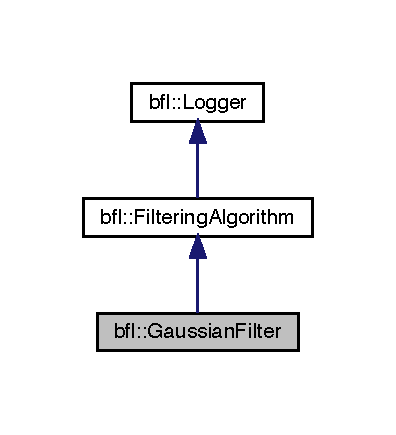
\includegraphics[width=190pt]{classbfl_1_1GaussianFilter__inherit__graph}
\end{center}
\end{figure}
\subsection*{Public Member Functions}
\begin{DoxyCompactItemize}
\item 
\mbox{\hyperlink{classbfl_1_1GaussianFilter_a480ea4178578324e2805f93884b718f1}{Gaussian\+Filter}} (\mbox{\hyperlink{classbfl_1_1Gaussian}{Gaussian}} \&initial\+\_\+state, std\+::unique\+\_\+ptr$<$ \mbox{\hyperlink{classbfl_1_1GaussianPrediction}{Gaussian\+Prediction}} $>$ prediction, std\+::unique\+\_\+ptr$<$ \mbox{\hyperlink{classbfl_1_1GaussianCorrection}{Gaussian\+Correction}} $>$ correction) noexcept
\item 
\mbox{\hyperlink{classbfl_1_1GaussianFilter_a322f9780479ab3c841f417e496783c9b}{Gaussian\+Filter}} (\mbox{\hyperlink{classbfl_1_1GaussianFilter}{Gaussian\+Filter}} \&\&kf) noexcept
\item 
\mbox{\hyperlink{classbfl_1_1GaussianFilter}{Gaussian\+Filter}} \& \mbox{\hyperlink{classbfl_1_1GaussianFilter_a9ce91b240bd88f83a6eba8f01e4b34eb}{operator=}} (\mbox{\hyperlink{classbfl_1_1GaussianFilter}{Gaussian\+Filter}} \&\&gf) noexcept
\item 
virtual \mbox{\hyperlink{classbfl_1_1GaussianFilter_a1d8226f8fe6f3f87ef0b71cc0579968f}{$\sim$\+Gaussian\+Filter}} () noexcept
\item 
bool \mbox{\hyperlink{classbfl_1_1GaussianFilter_ac0305fa835af89ba5962ee1211d4d0c0}{initialization}} () override
\item 
void \mbox{\hyperlink{classbfl_1_1GaussianFilter_ae30a175454a93685eca79d3ef857f7bc}{filtering\+Step}} () override
\item 
bool \mbox{\hyperlink{classbfl_1_1GaussianFilter_acf6902f6156c573560b57f10c1992b8a}{run\+Condition}} () override
\item 
bool \mbox{\hyperlink{classbfl_1_1GaussianFilter_a3ca79ee1451863d898baeea6a74ababd}{skip}} (const std\+::string \&what\+\_\+step, const bool status) override
\item 
bool \mbox{\hyperlink{classbfl_1_1FilteringAlgorithm_a96651f8464190c0a56d79219a1017147}{boot}} ()
\item 
void \mbox{\hyperlink{classbfl_1_1FilteringAlgorithm_a009cbe5f4bbb16967f6c6ddcaed8fbb1}{run}} ()
\item 
bool \mbox{\hyperlink{classbfl_1_1FilteringAlgorithm_a40372c24fa050eb0274371172df0a244}{wait}} ()
\item 
void \mbox{\hyperlink{classbfl_1_1FilteringAlgorithm_a2403c62fbd7bd7f5cda56a84f5f30331}{reset}} ()
\item 
void \mbox{\hyperlink{classbfl_1_1FilteringAlgorithm_a6022859aa985474fb997343cc935b11e}{reboot}} ()
\item 
bool \mbox{\hyperlink{classbfl_1_1FilteringAlgorithm_a1dc912d89ee8f96d4f3e8209865c5308}{teardown}} ()
\item 
unsigned int \mbox{\hyperlink{classbfl_1_1FilteringAlgorithm_a8c43b1f3dac30934c0a03de348d4a29d}{get\+Filtering\+Step}} ()
\item 
bool \mbox{\hyperlink{classbfl_1_1FilteringAlgorithm_a5cfecab2c778620e2557237472bb1721}{is\+Running}} ()
\item 
bool \mbox{\hyperlink{classbfl_1_1Logger_ae94b97b6e8d7902e8ce048384813122e}{enable\+\_\+log}} (const std\+::string \&prefix\+\_\+path, const std\+::string \&prefix\+\_\+name)
\item 
bool \mbox{\hyperlink{classbfl_1_1Logger_a440467a28ccc46490d767fe0ef6f556a}{disable\+\_\+log}} ()
\item 
std\+::string \mbox{\hyperlink{classbfl_1_1Logger_a56cf1a4e712bf23d9978420a8a59a62b}{get\+\_\+prefix\+\_\+path}} () const
\item 
std\+::string \mbox{\hyperlink{classbfl_1_1Logger_a913a795b7bfbf378815eeb342d68a7c0}{get\+\_\+prefix\+\_\+name}} () const
\item 
{\footnotesize template$<$typename Datum\+Type $>$ }\\void \mbox{\hyperlink{classbfl_1_1Logger_a1033ff31398484f2132f84fd140da9e3}{logger}} (Datum\+Type datum)
\item 
{\footnotesize template$<$typename... Data\+Type$>$ }\\void \mbox{\hyperlink{classbfl_1_1Logger_aca2086c9256e5c404872b91f7f25b97d}{logger}} (Data\+Type... data)
\item 
{\footnotesize template$<$typename Datum\+Type $>$ }\\void \mbox{\hyperlink{classbfl_1_1Logger_a50b1c109730fa98f66e66f420f0158fe}{logger}} (Datum\+Type datum) const
\item 
{\footnotesize template$<$typename... Data\+Type$>$ }\\void \mbox{\hyperlink{classbfl_1_1Logger_a0f0cf7ce956546d94dfb1feb7cebf171}{logger}} (Data\+Type... data) const
\end{DoxyCompactItemize}
\subsection*{Protected Member Functions}
\begin{DoxyCompactItemize}
\item 
virtual std\+::vector$<$ std\+::string $>$ \mbox{\hyperlink{classbfl_1_1Logger_a328ceaa8e70e6918f11142b12b8be217}{log\+\_\+filenames}} (const std\+::string \&prefix\+\_\+path, const std\+::string \&prefix\+\_\+name)
\item 
virtual void \mbox{\hyperlink{classbfl_1_1Logger_ad44f46593cb8c4c87c1178eb326e2f64}{log}} ()
\end{DoxyCompactItemize}
\subsection*{Protected Attributes}
\begin{DoxyCompactItemize}
\item 
\mbox{\hyperlink{classbfl_1_1Gaussian}{Gaussian}} \mbox{\hyperlink{classbfl_1_1GaussianFilter_a2a1d0665d3bec12be129b33d06098ca4}{predicted\+\_\+state\+\_\+}}
\item 
\mbox{\hyperlink{classbfl_1_1Gaussian}{Gaussian}} \mbox{\hyperlink{classbfl_1_1GaussianFilter_a7b653083e75369f0e0d0436ed4ddcbca}{corrected\+\_\+state\+\_\+}}
\item 
std\+::unique\+\_\+ptr$<$ \mbox{\hyperlink{classbfl_1_1GaussianPrediction}{Gaussian\+Prediction}} $>$ \mbox{\hyperlink{classbfl_1_1GaussianFilter_a407bf3e926711e771304a8aaeb4db863}{prediction\+\_\+}}
\item 
std\+::unique\+\_\+ptr$<$ \mbox{\hyperlink{classbfl_1_1GaussianCorrection}{Gaussian\+Correction}} $>$ \mbox{\hyperlink{classbfl_1_1GaussianFilter_aec8fd5bd317c76fc133296b6e544d0b0}{correction\+\_\+}}
\end{DoxyCompactItemize}


\subsection{Detailed Description}


Definition at line 14 of file Gaussian\+Filter.\+h.



\subsection{Constructor \& Destructor Documentation}
\mbox{\Hypertarget{classbfl_1_1GaussianFilter_a480ea4178578324e2805f93884b718f1}\label{classbfl_1_1GaussianFilter_a480ea4178578324e2805f93884b718f1}} 
\index{bfl\+::\+Gaussian\+Filter@{bfl\+::\+Gaussian\+Filter}!Gaussian\+Filter@{Gaussian\+Filter}}
\index{Gaussian\+Filter@{Gaussian\+Filter}!bfl\+::\+Gaussian\+Filter@{bfl\+::\+Gaussian\+Filter}}
\subsubsection{\texorpdfstring{Gaussian\+Filter()}{GaussianFilter()}\hspace{0.1cm}{\footnotesize\ttfamily [1/2]}}
{\footnotesize\ttfamily Gaussian\+Filter\+::\+Gaussian\+Filter (\begin{DoxyParamCaption}\item[{\mbox{\hyperlink{classbfl_1_1Gaussian}{Gaussian}} \&}]{initial\+\_\+state,  }\item[{std\+::unique\+\_\+ptr$<$ \mbox{\hyperlink{classbfl_1_1GaussianPrediction}{Gaussian\+Prediction}} $>$}]{prediction,  }\item[{std\+::unique\+\_\+ptr$<$ \mbox{\hyperlink{classbfl_1_1GaussianCorrection}{Gaussian\+Correction}} $>$}]{correction }\end{DoxyParamCaption})\hspace{0.3cm}{\ttfamily [noexcept]}}



Definition at line 7 of file Gaussian\+Filter.\+cpp.

\mbox{\Hypertarget{classbfl_1_1GaussianFilter_a322f9780479ab3c841f417e496783c9b}\label{classbfl_1_1GaussianFilter_a322f9780479ab3c841f417e496783c9b}} 
\index{bfl\+::\+Gaussian\+Filter@{bfl\+::\+Gaussian\+Filter}!Gaussian\+Filter@{Gaussian\+Filter}}
\index{Gaussian\+Filter@{Gaussian\+Filter}!bfl\+::\+Gaussian\+Filter@{bfl\+::\+Gaussian\+Filter}}
\subsubsection{\texorpdfstring{Gaussian\+Filter()}{GaussianFilter()}\hspace{0.1cm}{\footnotesize\ttfamily [2/2]}}
{\footnotesize\ttfamily Gaussian\+Filter\+::\+Gaussian\+Filter (\begin{DoxyParamCaption}\item[{\mbox{\hyperlink{classbfl_1_1GaussianFilter}{Gaussian\+Filter}} \&\&}]{kf }\end{DoxyParamCaption})\hspace{0.3cm}{\ttfamily [noexcept]}}



Definition at line 19 of file Gaussian\+Filter.\+cpp.

\mbox{\Hypertarget{classbfl_1_1GaussianFilter_a1d8226f8fe6f3f87ef0b71cc0579968f}\label{classbfl_1_1GaussianFilter_a1d8226f8fe6f3f87ef0b71cc0579968f}} 
\index{bfl\+::\+Gaussian\+Filter@{bfl\+::\+Gaussian\+Filter}!````~Gaussian\+Filter@{$\sim$\+Gaussian\+Filter}}
\index{````~Gaussian\+Filter@{$\sim$\+Gaussian\+Filter}!bfl\+::\+Gaussian\+Filter@{bfl\+::\+Gaussian\+Filter}}
\subsubsection{\texorpdfstring{$\sim$\+Gaussian\+Filter()}{~GaussianFilter()}}
{\footnotesize\ttfamily Gaussian\+Filter\+::$\sim$\+Gaussian\+Filter (\begin{DoxyParamCaption}{ }\end{DoxyParamCaption})\hspace{0.3cm}{\ttfamily [virtual]}, {\ttfamily [noexcept]}}



Definition at line 27 of file Gaussian\+Filter.\+cpp.



\subsection{Member Function Documentation}
\mbox{\Hypertarget{classbfl_1_1FilteringAlgorithm_a96651f8464190c0a56d79219a1017147}\label{classbfl_1_1FilteringAlgorithm_a96651f8464190c0a56d79219a1017147}} 
\index{bfl\+::\+Gaussian\+Filter@{bfl\+::\+Gaussian\+Filter}!boot@{boot}}
\index{boot@{boot}!bfl\+::\+Gaussian\+Filter@{bfl\+::\+Gaussian\+Filter}}
\subsubsection{\texorpdfstring{boot()}{boot()}}
{\footnotesize\ttfamily bool Filtering\+Algorithm\+::boot (\begin{DoxyParamCaption}{ }\end{DoxyParamCaption})\hspace{0.3cm}{\ttfamily [inherited]}}



Definition at line 8 of file Filtering\+Algorithm.\+cpp.



References bfl\+::\+Filtering\+Algorithm\+::filtering\+\_\+thread\+\_\+, and bfl\+::\+Filtering\+Algorithm\+::filtering\+Recursion().

Here is the call graph for this function\+:
\nopagebreak
\begin{figure}[H]
\begin{center}
\leavevmode
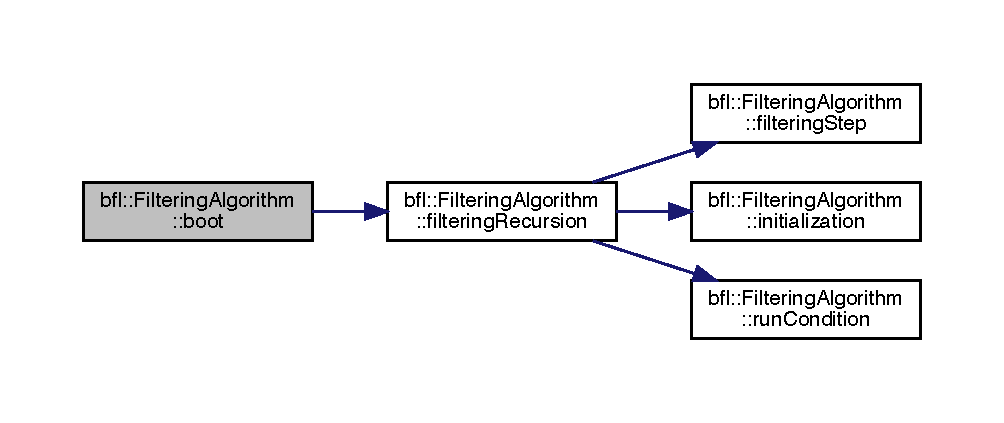
\includegraphics[width=350pt]{classbfl_1_1FilteringAlgorithm_a96651f8464190c0a56d79219a1017147_cgraph}
\end{center}
\end{figure}
\mbox{\Hypertarget{classbfl_1_1Logger_a440467a28ccc46490d767fe0ef6f556a}\label{classbfl_1_1Logger_a440467a28ccc46490d767fe0ef6f556a}} 
\index{bfl\+::\+Gaussian\+Filter@{bfl\+::\+Gaussian\+Filter}!disable\+\_\+log@{disable\+\_\+log}}
\index{disable\+\_\+log@{disable\+\_\+log}!bfl\+::\+Gaussian\+Filter@{bfl\+::\+Gaussian\+Filter}}
\subsubsection{\texorpdfstring{disable\+\_\+log()}{disable\_log()}}
{\footnotesize\ttfamily bool Logger\+::disable\+\_\+log (\begin{DoxyParamCaption}{ }\end{DoxyParamCaption})\hspace{0.3cm}{\ttfamily [inherited]}}



Definition at line 58 of file Logger.\+cpp.



References bfl\+::\+Logger\+::file\+\_\+names\+\_\+, bfl\+::\+Logger\+::log\+\_\+enabled\+\_\+, and bfl\+::\+Logger\+::log\+\_\+files\+\_\+.



Referenced by bfl\+::\+Logger\+::$\sim$\+Logger().

\mbox{\Hypertarget{classbfl_1_1Logger_ae94b97b6e8d7902e8ce048384813122e}\label{classbfl_1_1Logger_ae94b97b6e8d7902e8ce048384813122e}} 
\index{bfl\+::\+Gaussian\+Filter@{bfl\+::\+Gaussian\+Filter}!enable\+\_\+log@{enable\+\_\+log}}
\index{enable\+\_\+log@{enable\+\_\+log}!bfl\+::\+Gaussian\+Filter@{bfl\+::\+Gaussian\+Filter}}
\subsubsection{\texorpdfstring{enable\+\_\+log()}{enable\_log()}}
{\footnotesize\ttfamily bool Logger\+::enable\+\_\+log (\begin{DoxyParamCaption}\item[{const std\+::string \&}]{prefix\+\_\+path,  }\item[{const std\+::string \&}]{prefix\+\_\+name }\end{DoxyParamCaption})\hspace{0.3cm}{\ttfamily [inherited]}}



Definition at line 15 of file Logger.\+cpp.



References bfl\+::\+Logger\+::file\+\_\+names\+\_\+, bfl\+::\+Logger\+::log\+\_\+enabled\+\_\+, bfl\+::\+Logger\+::log\+\_\+filenames(), and bfl\+::\+Logger\+::log\+\_\+files\+\_\+.

Here is the call graph for this function\+:
\nopagebreak
\begin{figure}[H]
\begin{center}
\leavevmode
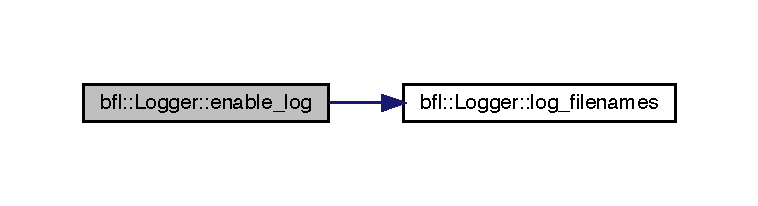
\includegraphics[width=350pt]{classbfl_1_1Logger_ae94b97b6e8d7902e8ce048384813122e_cgraph}
\end{center}
\end{figure}
\mbox{\Hypertarget{classbfl_1_1GaussianFilter_ae30a175454a93685eca79d3ef857f7bc}\label{classbfl_1_1GaussianFilter_ae30a175454a93685eca79d3ef857f7bc}} 
\index{bfl\+::\+Gaussian\+Filter@{bfl\+::\+Gaussian\+Filter}!filtering\+Step@{filtering\+Step}}
\index{filtering\+Step@{filtering\+Step}!bfl\+::\+Gaussian\+Filter@{bfl\+::\+Gaussian\+Filter}}
\subsubsection{\texorpdfstring{filtering\+Step()}{filteringStep()}}
{\footnotesize\ttfamily void Gaussian\+Filter\+::filtering\+Step (\begin{DoxyParamCaption}{ }\end{DoxyParamCaption})\hspace{0.3cm}{\ttfamily [override]}, {\ttfamily [virtual]}}



Implements \mbox{\hyperlink{classbfl_1_1FilteringAlgorithm_ab3bceb43b5810a4bf1da884b8a0b145a}{bfl\+::\+Filtering\+Algorithm}}.



Definition at line 37 of file Gaussian\+Filter.\+cpp.



References corrected\+\_\+state\+\_\+, correction\+\_\+, bfl\+::\+Logger\+::log(), predicted\+\_\+state\+\_\+, and prediction\+\_\+.

Here is the call graph for this function\+:
\nopagebreak
\begin{figure}[H]
\begin{center}
\leavevmode
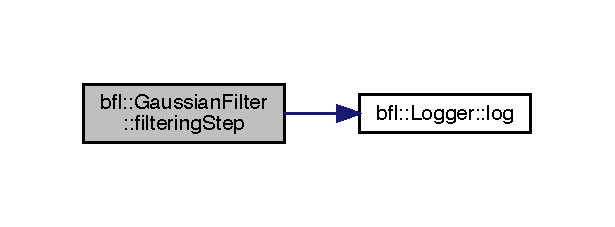
\includegraphics[width=295pt]{classbfl_1_1GaussianFilter_ae30a175454a93685eca79d3ef857f7bc_cgraph}
\end{center}
\end{figure}
\mbox{\Hypertarget{classbfl_1_1Logger_a913a795b7bfbf378815eeb342d68a7c0}\label{classbfl_1_1Logger_a913a795b7bfbf378815eeb342d68a7c0}} 
\index{bfl\+::\+Gaussian\+Filter@{bfl\+::\+Gaussian\+Filter}!get\+\_\+prefix\+\_\+name@{get\+\_\+prefix\+\_\+name}}
\index{get\+\_\+prefix\+\_\+name@{get\+\_\+prefix\+\_\+name}!bfl\+::\+Gaussian\+Filter@{bfl\+::\+Gaussian\+Filter}}
\subsubsection{\texorpdfstring{get\+\_\+prefix\+\_\+name()}{get\_prefix\_name()}}
{\footnotesize\ttfamily std\+::string Logger\+::get\+\_\+prefix\+\_\+name (\begin{DoxyParamCaption}{ }\end{DoxyParamCaption}) const\hspace{0.3cm}{\ttfamily [inherited]}}



Definition at line 81 of file Logger.\+cpp.



References bfl\+::\+Logger\+::prefix\+\_\+name\+\_\+.

\mbox{\Hypertarget{classbfl_1_1Logger_a56cf1a4e712bf23d9978420a8a59a62b}\label{classbfl_1_1Logger_a56cf1a4e712bf23d9978420a8a59a62b}} 
\index{bfl\+::\+Gaussian\+Filter@{bfl\+::\+Gaussian\+Filter}!get\+\_\+prefix\+\_\+path@{get\+\_\+prefix\+\_\+path}}
\index{get\+\_\+prefix\+\_\+path@{get\+\_\+prefix\+\_\+path}!bfl\+::\+Gaussian\+Filter@{bfl\+::\+Gaussian\+Filter}}
\subsubsection{\texorpdfstring{get\+\_\+prefix\+\_\+path()}{get\_prefix\_path()}}
{\footnotesize\ttfamily std\+::string Logger\+::get\+\_\+prefix\+\_\+path (\begin{DoxyParamCaption}{ }\end{DoxyParamCaption}) const\hspace{0.3cm}{\ttfamily [inherited]}}



Definition at line 75 of file Logger.\+cpp.



References bfl\+::\+Logger\+::prefix\+\_\+path\+\_\+.

\mbox{\Hypertarget{classbfl_1_1FilteringAlgorithm_a8c43b1f3dac30934c0a03de348d4a29d}\label{classbfl_1_1FilteringAlgorithm_a8c43b1f3dac30934c0a03de348d4a29d}} 
\index{bfl\+::\+Gaussian\+Filter@{bfl\+::\+Gaussian\+Filter}!get\+Filtering\+Step@{get\+Filtering\+Step}}
\index{get\+Filtering\+Step@{get\+Filtering\+Step}!bfl\+::\+Gaussian\+Filter@{bfl\+::\+Gaussian\+Filter}}
\subsubsection{\texorpdfstring{get\+Filtering\+Step()}{getFilteringStep()}}
{\footnotesize\ttfamily unsigned int Filtering\+Algorithm\+::get\+Filtering\+Step (\begin{DoxyParamCaption}{ }\end{DoxyParamCaption})\hspace{0.3cm}{\ttfamily [inherited]}}



Definition at line 83 of file Filtering\+Algorithm.\+cpp.



References bfl\+::\+Filtering\+Algorithm\+::filtering\+\_\+step\+\_\+.

\mbox{\Hypertarget{classbfl_1_1GaussianFilter_ac0305fa835af89ba5962ee1211d4d0c0}\label{classbfl_1_1GaussianFilter_ac0305fa835af89ba5962ee1211d4d0c0}} 
\index{bfl\+::\+Gaussian\+Filter@{bfl\+::\+Gaussian\+Filter}!initialization@{initialization}}
\index{initialization@{initialization}!bfl\+::\+Gaussian\+Filter@{bfl\+::\+Gaussian\+Filter}}
\subsubsection{\texorpdfstring{initialization()}{initialization()}}
{\footnotesize\ttfamily bool Gaussian\+Filter\+::initialization (\begin{DoxyParamCaption}{ }\end{DoxyParamCaption})\hspace{0.3cm}{\ttfamily [override]}, {\ttfamily [virtual]}}



Implements \mbox{\hyperlink{classbfl_1_1FilteringAlgorithm_adebe2ec2372f97a2a5baecf8c2c2a9c9}{bfl\+::\+Filtering\+Algorithm}}.



Definition at line 31 of file Gaussian\+Filter.\+cpp.

\mbox{\Hypertarget{classbfl_1_1FilteringAlgorithm_a5cfecab2c778620e2557237472bb1721}\label{classbfl_1_1FilteringAlgorithm_a5cfecab2c778620e2557237472bb1721}} 
\index{bfl\+::\+Gaussian\+Filter@{bfl\+::\+Gaussian\+Filter}!is\+Running@{is\+Running}}
\index{is\+Running@{is\+Running}!bfl\+::\+Gaussian\+Filter@{bfl\+::\+Gaussian\+Filter}}
\subsubsection{\texorpdfstring{is\+Running()}{isRunning()}}
{\footnotesize\ttfamily bool Filtering\+Algorithm\+::is\+Running (\begin{DoxyParamCaption}{ }\end{DoxyParamCaption})\hspace{0.3cm}{\ttfamily [inherited]}}



Definition at line 89 of file Filtering\+Algorithm.\+cpp.



References bfl\+::\+Filtering\+Algorithm\+::run\+\_\+.

\mbox{\Hypertarget{classbfl_1_1Logger_ad44f46593cb8c4c87c1178eb326e2f64}\label{classbfl_1_1Logger_ad44f46593cb8c4c87c1178eb326e2f64}} 
\index{bfl\+::\+Gaussian\+Filter@{bfl\+::\+Gaussian\+Filter}!log@{log}}
\index{log@{log}!bfl\+::\+Gaussian\+Filter@{bfl\+::\+Gaussian\+Filter}}
\subsubsection{\texorpdfstring{log()}{log()}}
{\footnotesize\ttfamily void Logger\+::log (\begin{DoxyParamCaption}{ }\end{DoxyParamCaption})\hspace{0.3cm}{\ttfamily [protected]}, {\ttfamily [virtual]}, {\ttfamily [inherited]}}



Reimplemented in \mbox{\hyperlink{classbfl_1_1SIS_aeb0b87af1cc1fc4b616989ef489ecccc}{bfl\+::\+S\+IS}}, \mbox{\hyperlink{classbfl_1_1SimulatedStateModel_aa022eb0d50d898ffcc831af2907265b2}{bfl\+::\+Simulated\+State\+Model}}, and \mbox{\hyperlink{classbfl_1_1SimulatedLinearSensor_ab75bbe744d8516c97dfc90ad499b10e6}{bfl\+::\+Simulated\+Linear\+Sensor}}.



Definition at line 99 of file Logger.\+cpp.



Referenced by filtering\+Step().

\mbox{\Hypertarget{classbfl_1_1Logger_a328ceaa8e70e6918f11142b12b8be217}\label{classbfl_1_1Logger_a328ceaa8e70e6918f11142b12b8be217}} 
\index{bfl\+::\+Gaussian\+Filter@{bfl\+::\+Gaussian\+Filter}!log\+\_\+filenames@{log\+\_\+filenames}}
\index{log\+\_\+filenames@{log\+\_\+filenames}!bfl\+::\+Gaussian\+Filter@{bfl\+::\+Gaussian\+Filter}}
\subsubsection{\texorpdfstring{log\+\_\+filenames()}{log\_filenames()}}
{\footnotesize\ttfamily std\+::vector$<$ std\+::string $>$ Logger\+::log\+\_\+filenames (\begin{DoxyParamCaption}\item[{const std\+::string \&}]{prefix\+\_\+path,  }\item[{const std\+::string \&}]{prefix\+\_\+name }\end{DoxyParamCaption})\hspace{0.3cm}{\ttfamily [protected]}, {\ttfamily [virtual]}, {\ttfamily [inherited]}}



Reimplemented in \mbox{\hyperlink{classbfl_1_1LinearModel_a8b8f645a7b7d8ebbb02c8958428fcf10}{bfl\+::\+Linear\+Model}}, \mbox{\hyperlink{classbfl_1_1SimulatedStateModel_ab4212871b8ca425855ec351c13dc3052}{bfl\+::\+Simulated\+State\+Model}}, and \mbox{\hyperlink{classbfl_1_1SIS_a805aef60946bfcaae4f65473dc7bd5ae}{bfl\+::\+S\+IS}}.



Definition at line 87 of file Logger.\+cpp.



Referenced by bfl\+::\+Logger\+::enable\+\_\+log().

\mbox{\Hypertarget{classbfl_1_1Logger_a1033ff31398484f2132f84fd140da9e3}\label{classbfl_1_1Logger_a1033ff31398484f2132f84fd140da9e3}} 
\index{bfl\+::\+Gaussian\+Filter@{bfl\+::\+Gaussian\+Filter}!logger@{logger}}
\index{logger@{logger}!bfl\+::\+Gaussian\+Filter@{bfl\+::\+Gaussian\+Filter}}
\subsubsection{\texorpdfstring{logger()}{logger()}\hspace{0.1cm}{\footnotesize\ttfamily [1/4]}}
{\footnotesize\ttfamily template$<$typename Datum\+Type $>$ \\
void bfl\+::\+Logger\+::logger (\begin{DoxyParamCaption}\item[{Datum\+Type}]{datum }\end{DoxyParamCaption})\hspace{0.3cm}{\ttfamily [inline]}, {\ttfamily [inherited]}}



Definition at line 28 of file Logger.\+h.



References bfl\+::\+Logger\+::log\+\_\+enabled\+\_\+, and bfl\+::\+Logger\+::log\+\_\+files\+\_\+.



Referenced by bfl\+::\+Simulated\+Linear\+Sensor\+::log().

\mbox{\Hypertarget{classbfl_1_1Logger_aca2086c9256e5c404872b91f7f25b97d}\label{classbfl_1_1Logger_aca2086c9256e5c404872b91f7f25b97d}} 
\index{bfl\+::\+Gaussian\+Filter@{bfl\+::\+Gaussian\+Filter}!logger@{logger}}
\index{logger@{logger}!bfl\+::\+Gaussian\+Filter@{bfl\+::\+Gaussian\+Filter}}
\subsubsection{\texorpdfstring{logger()}{logger()}\hspace{0.1cm}{\footnotesize\ttfamily [2/4]}}
{\footnotesize\ttfamily template$<$typename... Data\+Type$>$ \\
void bfl\+::\+Logger\+::logger (\begin{DoxyParamCaption}\item[{Data\+Type...}]{data }\end{DoxyParamCaption})\hspace{0.3cm}{\ttfamily [inline]}, {\ttfamily [inherited]}}



Definition at line 35 of file Logger.\+h.



References bfl\+::\+Logger\+::log\+\_\+enabled\+\_\+, and bfl\+::\+Logger\+::logger\+\_\+helper().

Here is the call graph for this function\+:
\nopagebreak
\begin{figure}[H]
\begin{center}
\leavevmode
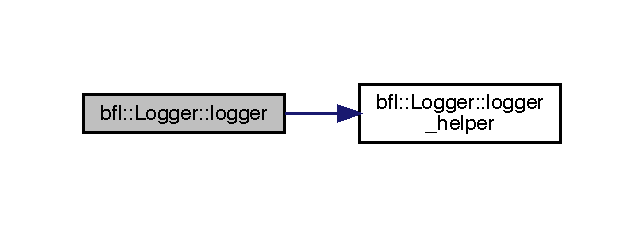
\includegraphics[width=309pt]{classbfl_1_1Logger_aca2086c9256e5c404872b91f7f25b97d_cgraph}
\end{center}
\end{figure}
\mbox{\Hypertarget{classbfl_1_1Logger_a50b1c109730fa98f66e66f420f0158fe}\label{classbfl_1_1Logger_a50b1c109730fa98f66e66f420f0158fe}} 
\index{bfl\+::\+Gaussian\+Filter@{bfl\+::\+Gaussian\+Filter}!logger@{logger}}
\index{logger@{logger}!bfl\+::\+Gaussian\+Filter@{bfl\+::\+Gaussian\+Filter}}
\subsubsection{\texorpdfstring{logger()}{logger()}\hspace{0.1cm}{\footnotesize\ttfamily [3/4]}}
{\footnotesize\ttfamily template$<$typename Datum\+Type $>$ \\
void bfl\+::\+Logger\+::logger (\begin{DoxyParamCaption}\item[{Datum\+Type}]{datum }\end{DoxyParamCaption}) const\hspace{0.3cm}{\ttfamily [inline]}, {\ttfamily [inherited]}}



Definition at line 42 of file Logger.\+h.



References bfl\+::\+Logger\+::log\+\_\+enabled\+\_\+, and bfl\+::\+Logger\+::log\+\_\+files\+\_\+.

\mbox{\Hypertarget{classbfl_1_1Logger_a0f0cf7ce956546d94dfb1feb7cebf171}\label{classbfl_1_1Logger_a0f0cf7ce956546d94dfb1feb7cebf171}} 
\index{bfl\+::\+Gaussian\+Filter@{bfl\+::\+Gaussian\+Filter}!logger@{logger}}
\index{logger@{logger}!bfl\+::\+Gaussian\+Filter@{bfl\+::\+Gaussian\+Filter}}
\subsubsection{\texorpdfstring{logger()}{logger()}\hspace{0.1cm}{\footnotesize\ttfamily [4/4]}}
{\footnotesize\ttfamily template$<$typename... Data\+Type$>$ \\
void bfl\+::\+Logger\+::logger (\begin{DoxyParamCaption}\item[{Data\+Type...}]{data }\end{DoxyParamCaption}) const\hspace{0.3cm}{\ttfamily [inline]}, {\ttfamily [inherited]}}



Definition at line 49 of file Logger.\+h.



References bfl\+::\+Logger\+::log\+\_\+enabled\+\_\+, and bfl\+::\+Logger\+::logger\+\_\+helper().

Here is the call graph for this function\+:
\nopagebreak
\begin{figure}[H]
\begin{center}
\leavevmode
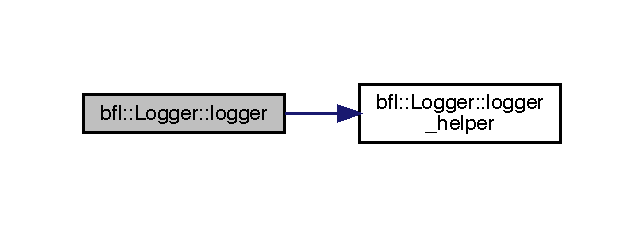
\includegraphics[width=309pt]{classbfl_1_1Logger_a0f0cf7ce956546d94dfb1feb7cebf171_cgraph}
\end{center}
\end{figure}
\mbox{\Hypertarget{classbfl_1_1GaussianFilter_a9ce91b240bd88f83a6eba8f01e4b34eb}\label{classbfl_1_1GaussianFilter_a9ce91b240bd88f83a6eba8f01e4b34eb}} 
\index{bfl\+::\+Gaussian\+Filter@{bfl\+::\+Gaussian\+Filter}!operator=@{operator=}}
\index{operator=@{operator=}!bfl\+::\+Gaussian\+Filter@{bfl\+::\+Gaussian\+Filter}}
\subsubsection{\texorpdfstring{operator=()}{operator=()}}
{\footnotesize\ttfamily \mbox{\hyperlink{classbfl_1_1GaussianFilter}{Gaussian\+Filter}}\& bfl\+::\+Gaussian\+Filter\+::operator= (\begin{DoxyParamCaption}\item[{\mbox{\hyperlink{classbfl_1_1GaussianFilter}{Gaussian\+Filter}} \&\&}]{gf }\end{DoxyParamCaption})\hspace{0.3cm}{\ttfamily [noexcept]}}

\mbox{\Hypertarget{classbfl_1_1FilteringAlgorithm_a6022859aa985474fb997343cc935b11e}\label{classbfl_1_1FilteringAlgorithm_a6022859aa985474fb997343cc935b11e}} 
\index{bfl\+::\+Gaussian\+Filter@{bfl\+::\+Gaussian\+Filter}!reboot@{reboot}}
\index{reboot@{reboot}!bfl\+::\+Gaussian\+Filter@{bfl\+::\+Gaussian\+Filter}}
\subsubsection{\texorpdfstring{reboot()}{reboot()}}
{\footnotesize\ttfamily void Filtering\+Algorithm\+::reboot (\begin{DoxyParamCaption}{ }\end{DoxyParamCaption})\hspace{0.3cm}{\ttfamily [inherited]}}



Definition at line 66 of file Filtering\+Algorithm.\+cpp.



References bfl\+::\+Filtering\+Algorithm\+::cv\+\_\+run\+\_\+, bfl\+::\+Filtering\+Algorithm\+::mtx\+\_\+run\+\_\+, bfl\+::\+Filtering\+Algorithm\+::reset\+\_\+, and bfl\+::\+Filtering\+Algorithm\+::run\+\_\+.

\mbox{\Hypertarget{classbfl_1_1FilteringAlgorithm_a2403c62fbd7bd7f5cda56a84f5f30331}\label{classbfl_1_1FilteringAlgorithm_a2403c62fbd7bd7f5cda56a84f5f30331}} 
\index{bfl\+::\+Gaussian\+Filter@{bfl\+::\+Gaussian\+Filter}!reset@{reset}}
\index{reset@{reset}!bfl\+::\+Gaussian\+Filter@{bfl\+::\+Gaussian\+Filter}}
\subsubsection{\texorpdfstring{reset()}{reset()}}
{\footnotesize\ttfamily void Filtering\+Algorithm\+::reset (\begin{DoxyParamCaption}{ }\end{DoxyParamCaption})\hspace{0.3cm}{\ttfamily [inherited]}}



Definition at line 60 of file Filtering\+Algorithm.\+cpp.



References bfl\+::\+Filtering\+Algorithm\+::reset\+\_\+.

\mbox{\Hypertarget{classbfl_1_1FilteringAlgorithm_a009cbe5f4bbb16967f6c6ddcaed8fbb1}\label{classbfl_1_1FilteringAlgorithm_a009cbe5f4bbb16967f6c6ddcaed8fbb1}} 
\index{bfl\+::\+Gaussian\+Filter@{bfl\+::\+Gaussian\+Filter}!run@{run}}
\index{run@{run}!bfl\+::\+Gaussian\+Filter@{bfl\+::\+Gaussian\+Filter}}
\subsubsection{\texorpdfstring{run()}{run()}}
{\footnotesize\ttfamily void Filtering\+Algorithm\+::run (\begin{DoxyParamCaption}{ }\end{DoxyParamCaption})\hspace{0.3cm}{\ttfamily [inherited]}}



Definition at line 26 of file Filtering\+Algorithm.\+cpp.



References bfl\+::\+Filtering\+Algorithm\+::cv\+\_\+run\+\_\+, bfl\+::\+Filtering\+Algorithm\+::mtx\+\_\+run\+\_\+, and bfl\+::\+Filtering\+Algorithm\+::run\+\_\+.

\mbox{\Hypertarget{classbfl_1_1GaussianFilter_acf6902f6156c573560b57f10c1992b8a}\label{classbfl_1_1GaussianFilter_acf6902f6156c573560b57f10c1992b8a}} 
\index{bfl\+::\+Gaussian\+Filter@{bfl\+::\+Gaussian\+Filter}!run\+Condition@{run\+Condition}}
\index{run\+Condition@{run\+Condition}!bfl\+::\+Gaussian\+Filter@{bfl\+::\+Gaussian\+Filter}}
\subsubsection{\texorpdfstring{run\+Condition()}{runCondition()}}
{\footnotesize\ttfamily bool Gaussian\+Filter\+::run\+Condition (\begin{DoxyParamCaption}{ }\end{DoxyParamCaption})\hspace{0.3cm}{\ttfamily [override]}, {\ttfamily [virtual]}}



Implements \mbox{\hyperlink{classbfl_1_1FilteringAlgorithm_a5fc12882356f6906b102fbfff2bc4b7c}{bfl\+::\+Filtering\+Algorithm}}.



Definition at line 46 of file Gaussian\+Filter.\+cpp.

\mbox{\Hypertarget{classbfl_1_1GaussianFilter_a3ca79ee1451863d898baeea6a74ababd}\label{classbfl_1_1GaussianFilter_a3ca79ee1451863d898baeea6a74ababd}} 
\index{bfl\+::\+Gaussian\+Filter@{bfl\+::\+Gaussian\+Filter}!skip@{skip}}
\index{skip@{skip}!bfl\+::\+Gaussian\+Filter@{bfl\+::\+Gaussian\+Filter}}
\subsubsection{\texorpdfstring{skip()}{skip()}}
{\footnotesize\ttfamily bool Gaussian\+Filter\+::skip (\begin{DoxyParamCaption}\item[{const std\+::string \&}]{what\+\_\+step,  }\item[{const bool}]{status }\end{DoxyParamCaption})\hspace{0.3cm}{\ttfamily [override]}, {\ttfamily [virtual]}}



Implements \mbox{\hyperlink{classbfl_1_1FilteringAlgorithm_ac8a718a614905d89d6a43bbbc70d68b2}{bfl\+::\+Filtering\+Algorithm}}.



Definition at line 52 of file Gaussian\+Filter.\+cpp.



References correction\+\_\+, and prediction\+\_\+.

\mbox{\Hypertarget{classbfl_1_1FilteringAlgorithm_a1dc912d89ee8f96d4f3e8209865c5308}\label{classbfl_1_1FilteringAlgorithm_a1dc912d89ee8f96d4f3e8209865c5308}} 
\index{bfl\+::\+Gaussian\+Filter@{bfl\+::\+Gaussian\+Filter}!teardown@{teardown}}
\index{teardown@{teardown}!bfl\+::\+Gaussian\+Filter@{bfl\+::\+Gaussian\+Filter}}
\subsubsection{\texorpdfstring{teardown()}{teardown()}}
{\footnotesize\ttfamily bool Filtering\+Algorithm\+::teardown (\begin{DoxyParamCaption}{ }\end{DoxyParamCaption})\hspace{0.3cm}{\ttfamily [inherited]}}



Definition at line 75 of file Filtering\+Algorithm.\+cpp.



References bfl\+::\+Filtering\+Algorithm\+::teardown\+\_\+.

\mbox{\Hypertarget{classbfl_1_1FilteringAlgorithm_a40372c24fa050eb0274371172df0a244}\label{classbfl_1_1FilteringAlgorithm_a40372c24fa050eb0274371172df0a244}} 
\index{bfl\+::\+Gaussian\+Filter@{bfl\+::\+Gaussian\+Filter}!wait@{wait}}
\index{wait@{wait}!bfl\+::\+Gaussian\+Filter@{bfl\+::\+Gaussian\+Filter}}
\subsubsection{\texorpdfstring{wait()}{wait()}}
{\footnotesize\ttfamily bool Filtering\+Algorithm\+::wait (\begin{DoxyParamCaption}{ }\end{DoxyParamCaption})\hspace{0.3cm}{\ttfamily [inherited]}}



Definition at line 34 of file Filtering\+Algorithm.\+cpp.



References bfl\+::\+Filtering\+Algorithm\+::filtering\+\_\+thread\+\_\+.



\subsection{Member Data Documentation}
\mbox{\Hypertarget{classbfl_1_1GaussianFilter_a7b653083e75369f0e0d0436ed4ddcbca}\label{classbfl_1_1GaussianFilter_a7b653083e75369f0e0d0436ed4ddcbca}} 
\index{bfl\+::\+Gaussian\+Filter@{bfl\+::\+Gaussian\+Filter}!corrected\+\_\+state\+\_\+@{corrected\+\_\+state\+\_\+}}
\index{corrected\+\_\+state\+\_\+@{corrected\+\_\+state\+\_\+}!bfl\+::\+Gaussian\+Filter@{bfl\+::\+Gaussian\+Filter}}
\subsubsection{\texorpdfstring{corrected\+\_\+state\+\_\+}{corrected\_state\_}}
{\footnotesize\ttfamily \mbox{\hyperlink{classbfl_1_1Gaussian}{Gaussian}} bfl\+::\+Gaussian\+Filter\+::corrected\+\_\+state\+\_\+\hspace{0.3cm}{\ttfamily [protected]}}



Definition at line 36 of file Gaussian\+Filter.\+h.



Referenced by filtering\+Step().

\mbox{\Hypertarget{classbfl_1_1GaussianFilter_aec8fd5bd317c76fc133296b6e544d0b0}\label{classbfl_1_1GaussianFilter_aec8fd5bd317c76fc133296b6e544d0b0}} 
\index{bfl\+::\+Gaussian\+Filter@{bfl\+::\+Gaussian\+Filter}!correction\+\_\+@{correction\+\_\+}}
\index{correction\+\_\+@{correction\+\_\+}!bfl\+::\+Gaussian\+Filter@{bfl\+::\+Gaussian\+Filter}}
\subsubsection{\texorpdfstring{correction\+\_\+}{correction\_}}
{\footnotesize\ttfamily std\+::unique\+\_\+ptr$<$\mbox{\hyperlink{classbfl_1_1GaussianCorrection}{Gaussian\+Correction}}$>$ bfl\+::\+Gaussian\+Filter\+::correction\+\_\+\hspace{0.3cm}{\ttfamily [protected]}}



Definition at line 40 of file Gaussian\+Filter.\+h.



Referenced by filtering\+Step(), and skip().

\mbox{\Hypertarget{classbfl_1_1GaussianFilter_a2a1d0665d3bec12be129b33d06098ca4}\label{classbfl_1_1GaussianFilter_a2a1d0665d3bec12be129b33d06098ca4}} 
\index{bfl\+::\+Gaussian\+Filter@{bfl\+::\+Gaussian\+Filter}!predicted\+\_\+state\+\_\+@{predicted\+\_\+state\+\_\+}}
\index{predicted\+\_\+state\+\_\+@{predicted\+\_\+state\+\_\+}!bfl\+::\+Gaussian\+Filter@{bfl\+::\+Gaussian\+Filter}}
\subsubsection{\texorpdfstring{predicted\+\_\+state\+\_\+}{predicted\_state\_}}
{\footnotesize\ttfamily \mbox{\hyperlink{classbfl_1_1Gaussian}{Gaussian}} bfl\+::\+Gaussian\+Filter\+::predicted\+\_\+state\+\_\+\hspace{0.3cm}{\ttfamily [protected]}}



Definition at line 34 of file Gaussian\+Filter.\+h.



Referenced by filtering\+Step().

\mbox{\Hypertarget{classbfl_1_1GaussianFilter_a407bf3e926711e771304a8aaeb4db863}\label{classbfl_1_1GaussianFilter_a407bf3e926711e771304a8aaeb4db863}} 
\index{bfl\+::\+Gaussian\+Filter@{bfl\+::\+Gaussian\+Filter}!prediction\+\_\+@{prediction\+\_\+}}
\index{prediction\+\_\+@{prediction\+\_\+}!bfl\+::\+Gaussian\+Filter@{bfl\+::\+Gaussian\+Filter}}
\subsubsection{\texorpdfstring{prediction\+\_\+}{prediction\_}}
{\footnotesize\ttfamily std\+::unique\+\_\+ptr$<$\mbox{\hyperlink{classbfl_1_1GaussianPrediction}{Gaussian\+Prediction}}$>$ bfl\+::\+Gaussian\+Filter\+::prediction\+\_\+\hspace{0.3cm}{\ttfamily [protected]}}



Definition at line 38 of file Gaussian\+Filter.\+h.



Referenced by filtering\+Step(), and skip().



The documentation for this class was generated from the following files\+:\begin{DoxyCompactItemize}
\item 
/\+Users/\+Claudio/\+Git\+Hub/bayes-\/filters-\/lib/src/\+Bayes\+Filters/include/\+Bayes\+Filters/\mbox{\hyperlink{GaussianFilter_8h}{Gaussian\+Filter.\+h}}\item 
/\+Users/\+Claudio/\+Git\+Hub/bayes-\/filters-\/lib/src/\+Bayes\+Filters/src/\mbox{\hyperlink{GaussianFilter_8cpp}{Gaussian\+Filter.\+cpp}}\end{DoxyCompactItemize}

\hypertarget{classbfl_1_1GaussianInitialization}{}\section{bfl\+:\+:Gaussian\+Initialization Class Reference}
\label{classbfl_1_1GaussianInitialization}\index{bfl\+::\+Gaussian\+Initialization@{bfl\+::\+Gaussian\+Initialization}}


{\ttfamily \#include $<$Gaussian\+Initialization.\+h$>$}

\subsection*{Public Member Functions}
\begin{DoxyCompactItemize}
\item 
virtual \mbox{\hyperlink{classbfl_1_1GaussianInitialization_a4a0d53cdc9eaa19f263eeff489d0a437}{$\sim$\+Gaussian\+Initialization}} () noexcept
\item 
virtual void \mbox{\hyperlink{classbfl_1_1GaussianInitialization_ae1ef36cd233e10547778b3b339009c69}{initialize}} (\mbox{\hyperlink{classbfl_1_1Gaussian}{Gaussian}} \&state)=0
\end{DoxyCompactItemize}


\subsection{Detailed Description}


Definition at line 13 of file Gaussian\+Initialization.\+h.



\subsection{Constructor \& Destructor Documentation}
\mbox{\Hypertarget{classbfl_1_1GaussianInitialization_a4a0d53cdc9eaa19f263eeff489d0a437}\label{classbfl_1_1GaussianInitialization_a4a0d53cdc9eaa19f263eeff489d0a437}} 
\index{bfl\+::\+Gaussian\+Initialization@{bfl\+::\+Gaussian\+Initialization}!````~Gaussian\+Initialization@{$\sim$\+Gaussian\+Initialization}}
\index{````~Gaussian\+Initialization@{$\sim$\+Gaussian\+Initialization}!bfl\+::\+Gaussian\+Initialization@{bfl\+::\+Gaussian\+Initialization}}
\subsubsection{\texorpdfstring{$\sim$\+Gaussian\+Initialization()}{~GaussianInitialization()}}
{\footnotesize\ttfamily virtual bfl\+::\+Gaussian\+Initialization\+::$\sim$\+Gaussian\+Initialization (\begin{DoxyParamCaption}{ }\end{DoxyParamCaption})\hspace{0.3cm}{\ttfamily [inline]}, {\ttfamily [virtual]}, {\ttfamily [noexcept]}}



Definition at line 16 of file Gaussian\+Initialization.\+h.



\subsection{Member Function Documentation}
\mbox{\Hypertarget{classbfl_1_1GaussianInitialization_ae1ef36cd233e10547778b3b339009c69}\label{classbfl_1_1GaussianInitialization_ae1ef36cd233e10547778b3b339009c69}} 
\index{bfl\+::\+Gaussian\+Initialization@{bfl\+::\+Gaussian\+Initialization}!initialize@{initialize}}
\index{initialize@{initialize}!bfl\+::\+Gaussian\+Initialization@{bfl\+::\+Gaussian\+Initialization}}
\subsubsection{\texorpdfstring{initialize()}{initialize()}}
{\footnotesize\ttfamily virtual void bfl\+::\+Gaussian\+Initialization\+::initialize (\begin{DoxyParamCaption}\item[{\mbox{\hyperlink{classbfl_1_1Gaussian}{Gaussian}} \&}]{state }\end{DoxyParamCaption})\hspace{0.3cm}{\ttfamily [pure virtual]}}



The documentation for this class was generated from the following file\+:\begin{DoxyCompactItemize}
\item 
/\+Users/\+Claudio/\+Git\+Hub/bayes-\/filters-\/lib/src/\+Bayes\+Filters/include/\+Bayes\+Filters/\mbox{\hyperlink{GaussianInitialization_8h}{Gaussian\+Initialization.\+h}}\end{DoxyCompactItemize}

\hypertarget{classbfl_1_1GaussianLikelihood}{}\section{bfl\+:\+:Gaussian\+Likelihood Class Reference}
\label{classbfl_1_1GaussianLikelihood}\index{bfl\+::\+Gaussian\+Likelihood@{bfl\+::\+Gaussian\+Likelihood}}


{\ttfamily \#include $<$Gaussian\+Likelihood.\+h$>$}



Inheritance diagram for bfl\+:\+:Gaussian\+Likelihood\+:
\nopagebreak
\begin{figure}[H]
\begin{center}
\leavevmode
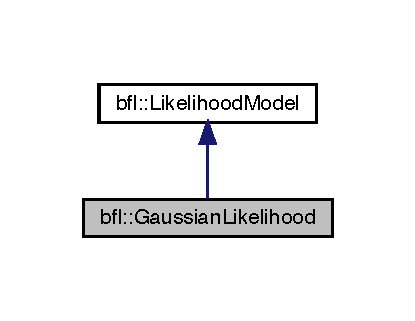
\includegraphics[width=199pt]{classbfl_1_1GaussianLikelihood__inherit__graph}
\end{center}
\end{figure}
\subsection*{Public Member Functions}
\begin{DoxyCompactItemize}
\item 
\mbox{\hyperlink{classbfl_1_1GaussianLikelihood_a431a2163fac8be200939266f28b62e6f}{Gaussian\+Likelihood}} () noexcept
\item 
\mbox{\hyperlink{classbfl_1_1GaussianLikelihood_ade56bbd79aa46bb5d97abcae2590489d}{Gaussian\+Likelihood}} (const double scale\+\_\+factor) noexcept
\item 
virtual \mbox{\hyperlink{classbfl_1_1GaussianLikelihood_a8d48eeeac83a3ac1a5e48913fdffa0d4}{$\sim$\+Gaussian\+Likelihood}} () noexcept
\end{DoxyCompactItemize}
\subsection*{Protected Member Functions}
\begin{DoxyCompactItemize}
\item 
std\+::pair$<$ bool, Eigen\+::\+Vector\+Xd $>$ \mbox{\hyperlink{classbfl_1_1GaussianLikelihood_a07bbe94864e1cf4ccb2232e51673575a}{likelihood}} (const \mbox{\hyperlink{classbfl_1_1MeasurementModel}{Measurement\+Model}} \&measurement\+\_\+model, const Eigen\+::\+Ref$<$ const Eigen\+::\+Matrix\+Xd $>$ \&pred\+\_\+states) override
\end{DoxyCompactItemize}
\subsection*{Protected Attributes}
\begin{DoxyCompactItemize}
\item 
double \mbox{\hyperlink{classbfl_1_1GaussianLikelihood_ad08436040da927c3a2bdeac9eab8aedf}{scale\+\_\+factor\+\_\+}}
\end{DoxyCompactItemize}


\subsection{Detailed Description}


Definition at line 11 of file Gaussian\+Likelihood.\+h.



\subsection{Constructor \& Destructor Documentation}
\mbox{\Hypertarget{classbfl_1_1GaussianLikelihood_a431a2163fac8be200939266f28b62e6f}\label{classbfl_1_1GaussianLikelihood_a431a2163fac8be200939266f28b62e6f}} 
\index{bfl\+::\+Gaussian\+Likelihood@{bfl\+::\+Gaussian\+Likelihood}!Gaussian\+Likelihood@{Gaussian\+Likelihood}}
\index{Gaussian\+Likelihood@{Gaussian\+Likelihood}!bfl\+::\+Gaussian\+Likelihood@{bfl\+::\+Gaussian\+Likelihood}}
\subsubsection{\texorpdfstring{Gaussian\+Likelihood()}{GaussianLikelihood()}\hspace{0.1cm}{\footnotesize\ttfamily [1/2]}}
{\footnotesize\ttfamily Gaussian\+Likelihood\+::\+Gaussian\+Likelihood (\begin{DoxyParamCaption}{ }\end{DoxyParamCaption})\hspace{0.3cm}{\ttfamily [noexcept]}}



Definition at line 7 of file Gaussian\+Likelihood.\+cpp.

\mbox{\Hypertarget{classbfl_1_1GaussianLikelihood_ade56bbd79aa46bb5d97abcae2590489d}\label{classbfl_1_1GaussianLikelihood_ade56bbd79aa46bb5d97abcae2590489d}} 
\index{bfl\+::\+Gaussian\+Likelihood@{bfl\+::\+Gaussian\+Likelihood}!Gaussian\+Likelihood@{Gaussian\+Likelihood}}
\index{Gaussian\+Likelihood@{Gaussian\+Likelihood}!bfl\+::\+Gaussian\+Likelihood@{bfl\+::\+Gaussian\+Likelihood}}
\subsubsection{\texorpdfstring{Gaussian\+Likelihood()}{GaussianLikelihood()}\hspace{0.1cm}{\footnotesize\ttfamily [2/2]}}
{\footnotesize\ttfamily Gaussian\+Likelihood\+::\+Gaussian\+Likelihood (\begin{DoxyParamCaption}\item[{const double}]{scale\+\_\+factor }\end{DoxyParamCaption})\hspace{0.3cm}{\ttfamily [noexcept]}}



Definition at line 11 of file Gaussian\+Likelihood.\+cpp.

\mbox{\Hypertarget{classbfl_1_1GaussianLikelihood_a8d48eeeac83a3ac1a5e48913fdffa0d4}\label{classbfl_1_1GaussianLikelihood_a8d48eeeac83a3ac1a5e48913fdffa0d4}} 
\index{bfl\+::\+Gaussian\+Likelihood@{bfl\+::\+Gaussian\+Likelihood}!````~Gaussian\+Likelihood@{$\sim$\+Gaussian\+Likelihood}}
\index{````~Gaussian\+Likelihood@{$\sim$\+Gaussian\+Likelihood}!bfl\+::\+Gaussian\+Likelihood@{bfl\+::\+Gaussian\+Likelihood}}
\subsubsection{\texorpdfstring{$\sim$\+Gaussian\+Likelihood()}{~GaussianLikelihood()}}
{\footnotesize\ttfamily virtual bfl\+::\+Gaussian\+Likelihood\+::$\sim$\+Gaussian\+Likelihood (\begin{DoxyParamCaption}{ }\end{DoxyParamCaption})\hspace{0.3cm}{\ttfamily [inline]}, {\ttfamily [virtual]}, {\ttfamily [noexcept]}}



Definition at line 18 of file Gaussian\+Likelihood.\+h.



\subsection{Member Function Documentation}
\mbox{\Hypertarget{classbfl_1_1GaussianLikelihood_a07bbe94864e1cf4ccb2232e51673575a}\label{classbfl_1_1GaussianLikelihood_a07bbe94864e1cf4ccb2232e51673575a}} 
\index{bfl\+::\+Gaussian\+Likelihood@{bfl\+::\+Gaussian\+Likelihood}!likelihood@{likelihood}}
\index{likelihood@{likelihood}!bfl\+::\+Gaussian\+Likelihood@{bfl\+::\+Gaussian\+Likelihood}}
\subsubsection{\texorpdfstring{likelihood()}{likelihood()}}
{\footnotesize\ttfamily std\+::pair$<$ bool, Vector\+Xd $>$ Gaussian\+Likelihood\+::likelihood (\begin{DoxyParamCaption}\item[{const \mbox{\hyperlink{classbfl_1_1MeasurementModel}{Measurement\+Model}} \&}]{measurement\+\_\+model,  }\item[{const Eigen\+::\+Ref$<$ const Eigen\+::\+Matrix\+Xd $>$ \&}]{pred\+\_\+states }\end{DoxyParamCaption})\hspace{0.3cm}{\ttfamily [override]}, {\ttfamily [protected]}, {\ttfamily [virtual]}}



Implements \mbox{\hyperlink{classbfl_1_1LikelihoodModel_a401a363bea9178f568ca4968f9d170b0}{bfl\+::\+Likelihood\+Model}}.



Definition at line 16 of file Gaussian\+Likelihood.\+cpp.



References bfl\+::any\+::any\+\_\+cast(), bfl\+::\+Measurement\+Model\+::get\+Noise\+Covariance\+Matrix(), bfl\+::\+Measurement\+Model\+::innovation(), bfl\+::\+Measurement\+Model\+::measure(), and bfl\+::\+Measurement\+Model\+::predicted\+Measure().

Here is the call graph for this function\+:
\nopagebreak
\begin{figure}[H]
\begin{center}
\leavevmode
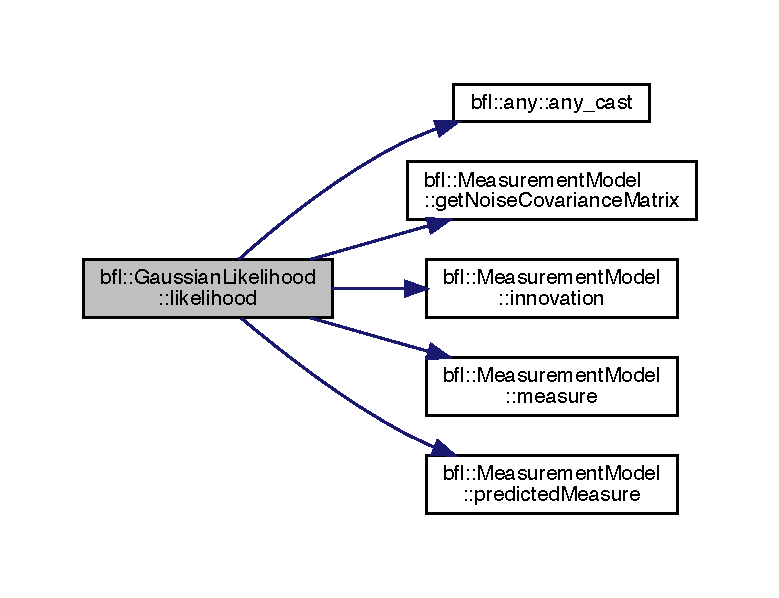
\includegraphics[width=350pt]{classbfl_1_1GaussianLikelihood_a07bbe94864e1cf4ccb2232e51673575a_cgraph}
\end{center}
\end{figure}


\subsection{Member Data Documentation}
\mbox{\Hypertarget{classbfl_1_1GaussianLikelihood_ad08436040da927c3a2bdeac9eab8aedf}\label{classbfl_1_1GaussianLikelihood_ad08436040da927c3a2bdeac9eab8aedf}} 
\index{bfl\+::\+Gaussian\+Likelihood@{bfl\+::\+Gaussian\+Likelihood}!scale\+\_\+factor\+\_\+@{scale\+\_\+factor\+\_\+}}
\index{scale\+\_\+factor\+\_\+@{scale\+\_\+factor\+\_\+}!bfl\+::\+Gaussian\+Likelihood@{bfl\+::\+Gaussian\+Likelihood}}
\subsubsection{\texorpdfstring{scale\+\_\+factor\+\_\+}{scale\_factor\_}}
{\footnotesize\ttfamily double bfl\+::\+Gaussian\+Likelihood\+::scale\+\_\+factor\+\_\+\hspace{0.3cm}{\ttfamily [protected]}}



Definition at line 23 of file Gaussian\+Likelihood.\+h.



The documentation for this class was generated from the following files\+:\begin{DoxyCompactItemize}
\item 
/\+Users/\+Claudio/\+Git\+Hub/bayes-\/filters-\/lib/src/\+Bayes\+Filters/include/\+Bayes\+Filters/\mbox{\hyperlink{GaussianLikelihood_8h}{Gaussian\+Likelihood.\+h}}\item 
/\+Users/\+Claudio/\+Git\+Hub/bayes-\/filters-\/lib/src/\+Bayes\+Filters/src/\mbox{\hyperlink{GaussianLikelihood_8cpp}{Gaussian\+Likelihood.\+cpp}}\end{DoxyCompactItemize}

\hypertarget{classbfl_1_1GaussianMixture}{}\section{bfl\+:\+:Gaussian\+Mixture Class Reference}
\label{classbfl_1_1GaussianMixture}\index{bfl\+::\+Gaussian\+Mixture@{bfl\+::\+Gaussian\+Mixture}}


{\ttfamily \#include $<$Gaussian\+Mixture.\+h$>$}



Inheritance diagram for bfl\+:\+:Gaussian\+Mixture\+:
\nopagebreak
\begin{figure}[H]
\begin{center}
\leavevmode
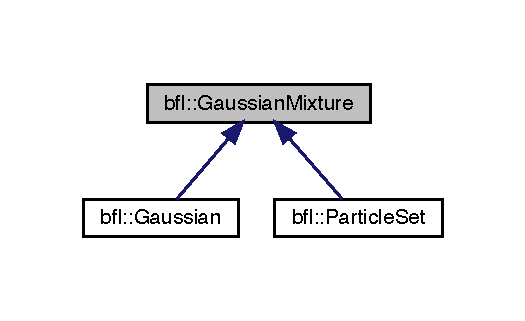
\includegraphics[width=252pt]{classbfl_1_1GaussianMixture__inherit__graph}
\end{center}
\end{figure}
\subsection*{Public Member Functions}
\begin{DoxyCompactItemize}
\item 
\mbox{\hyperlink{classbfl_1_1GaussianMixture_a0822b81102146cd9ba62223e41c97b38}{Gaussian\+Mixture}} ()
\item 
\mbox{\hyperlink{classbfl_1_1GaussianMixture_af2433812cdb02ca97c9cf6726683d31a}{Gaussian\+Mixture}} (const std\+::size\+\_\+t \mbox{\hyperlink{classbfl_1_1GaussianMixture_a02cc284327dbaa6b90c653dd2faccf88}{components}}, const std\+::size\+\_\+t \mbox{\hyperlink{classbfl_1_1GaussianMixture_a3f2b18801e72fa3bf0d6edc778662a8d}{dim}})
\item 
\mbox{\hyperlink{classbfl_1_1GaussianMixture_ab23a7e5d3646152dbd75cf50651ef896}{Gaussian\+Mixture}} (const std\+::size\+\_\+t \mbox{\hyperlink{classbfl_1_1GaussianMixture_a02cc284327dbaa6b90c653dd2faccf88}{components}}, const std\+::size\+\_\+t \mbox{\hyperlink{classbfl_1_1GaussianMixture_a22a0fbc77f90d9d75e89d7898484c05a}{dim\+\_\+linear}}, const std\+::size\+\_\+t \mbox{\hyperlink{classbfl_1_1GaussianMixture_a23f3b92753266475a9bff8ee7e1c9518}{dim\+\_\+circular}})
\item 
virtual \mbox{\hyperlink{classbfl_1_1GaussianMixture_aec7b09d8d2da90388879500466d4d349}{$\sim$\+Gaussian\+Mixture}} () noexcept
\item 
Eigen\+::\+Ref$<$ Eigen\+::\+Matrix\+Xd $>$ \mbox{\hyperlink{classbfl_1_1GaussianMixture_af4fd865a97ac27c72510cfbf9429bd97}{mean}} ()
\item 
Eigen\+::\+Ref$<$ Eigen\+::\+Vector\+Xd $>$ \mbox{\hyperlink{classbfl_1_1GaussianMixture_ad57440f7d524e5129afe70fc36f4fe99}{mean}} (const std\+::size\+\_\+t i)
\item 
double \& \mbox{\hyperlink{classbfl_1_1GaussianMixture_a21013d54d99ca5bfd1ec566a0815821e}{mean}} (const std\+::size\+\_\+t i, const std\+::size\+\_\+t j)
\item 
const Eigen\+::\+Ref$<$ const Eigen\+::\+Matrix\+Xd $>$ \mbox{\hyperlink{classbfl_1_1GaussianMixture_ad420f06f7680003453f64fd18bbb67da}{mean}} () const
\item 
const Eigen\+::\+Ref$<$ const Eigen\+::\+Vector\+Xd $>$ \mbox{\hyperlink{classbfl_1_1GaussianMixture_ad0dab37b16097d498dedaf23d0af3c18}{mean}} (const std\+::size\+\_\+t i) const
\item 
const double \& \mbox{\hyperlink{classbfl_1_1GaussianMixture_ac3baa237bc22f156f57d4c02deb4f518}{mean}} (const std\+::size\+\_\+t i, const std\+::size\+\_\+t j) const
\item 
Eigen\+::\+Ref$<$ Eigen\+::\+Matrix\+Xd $>$ \mbox{\hyperlink{classbfl_1_1GaussianMixture_a65a60ef46d16ac33196a09963bbccdee}{covariance}} ()
\item 
Eigen\+::\+Ref$<$ Eigen\+::\+Matrix\+Xd $>$ \mbox{\hyperlink{classbfl_1_1GaussianMixture_a80a6fa7d9edfc95103236378b4da3f7f}{covariance}} (const std\+::size\+\_\+t i)
\item 
double \& \mbox{\hyperlink{classbfl_1_1GaussianMixture_ad2c74407e682e3b4322df2d0e1cef28e}{covariance}} (const std\+::size\+\_\+t i, const std\+::size\+\_\+t j, const std\+::size\+\_\+t k)
\item 
const Eigen\+::\+Ref$<$ const Eigen\+::\+Matrix\+Xd $>$ \mbox{\hyperlink{classbfl_1_1GaussianMixture_a172c11264e6ff449a44ec21701eadc4d}{covariance}} () const
\item 
const Eigen\+::\+Ref$<$ const Eigen\+::\+Matrix\+Xd $>$ \mbox{\hyperlink{classbfl_1_1GaussianMixture_a3cff0f507ed950fe6a5e0aba1bf8467a}{covariance}} (const std\+::size\+\_\+t i) const
\item 
const double \& \mbox{\hyperlink{classbfl_1_1GaussianMixture_a4ca0b098be0fc923f454e73e9dccf78f}{covariance}} (const std\+::size\+\_\+t i, const std\+::size\+\_\+t j, const std\+::size\+\_\+t k) const
\item 
Eigen\+::\+Ref$<$ Eigen\+::\+Vector\+Xd $>$ \mbox{\hyperlink{classbfl_1_1GaussianMixture_ada5625de6a3e2f98afb5aaa148503dad}{weight}} ()
\item 
double \& \mbox{\hyperlink{classbfl_1_1GaussianMixture_a44885fb208e33f37015d47f55d02ef50}{weight}} (const std\+::size\+\_\+t i)
\item 
const Eigen\+::\+Ref$<$ const Eigen\+::\+Vector\+Xd $>$ \mbox{\hyperlink{classbfl_1_1GaussianMixture_a9ef04270bbccfe01f481665a1f390167}{weight}} () const
\item 
const double \& \mbox{\hyperlink{classbfl_1_1GaussianMixture_a42672f88d9126f018715a4d258a57731}{weight}} (const std\+::size\+\_\+t i) const
\item 
bool \mbox{\hyperlink{classbfl_1_1GaussianMixture_aec4e807341e18c18faed041c41121cb7}{augment\+With\+Noise}} (const Eigen\+::\+Ref$<$ const Eigen\+::\+Matrix\+Xd $>$ \&noise\+\_\+covariance\+\_\+matrix)
\end{DoxyCompactItemize}
\subsection*{Public Attributes}
\begin{DoxyCompactItemize}
\item 
std\+::size\+\_\+t \mbox{\hyperlink{classbfl_1_1GaussianMixture_a02cc284327dbaa6b90c653dd2faccf88}{components}}
\item 
std\+::size\+\_\+t \mbox{\hyperlink{classbfl_1_1GaussianMixture_a3f2b18801e72fa3bf0d6edc778662a8d}{dim}}
\item 
std\+::size\+\_\+t \mbox{\hyperlink{classbfl_1_1GaussianMixture_a22a0fbc77f90d9d75e89d7898484c05a}{dim\+\_\+linear}}
\item 
std\+::size\+\_\+t \mbox{\hyperlink{classbfl_1_1GaussianMixture_a23f3b92753266475a9bff8ee7e1c9518}{dim\+\_\+circular}}
\item 
std\+::size\+\_\+t \mbox{\hyperlink{classbfl_1_1GaussianMixture_adaa8d9c6d03be835769cc848aba81067}{dim\+\_\+noise}}
\end{DoxyCompactItemize}
\subsection*{Protected Attributes}
\begin{DoxyCompactItemize}
\item 
Eigen\+::\+Matrix\+Xd \mbox{\hyperlink{classbfl_1_1GaussianMixture_a12a1175e838a753129f4cc133b2c1a9c}{mean\+\_\+}}
\item 
Eigen\+::\+Matrix\+Xd \mbox{\hyperlink{classbfl_1_1GaussianMixture_aab086cc1a89a8b7efd15303853e52920}{covariance\+\_\+}}
\item 
Eigen\+::\+Vector\+Xd \mbox{\hyperlink{classbfl_1_1GaussianMixture_ac9ce000575d6b29ad8e1a756d750faff}{weight\+\_\+}}
\end{DoxyCompactItemize}


\subsection{Detailed Description}


Definition at line 13 of file Gaussian\+Mixture.\+h.



\subsection{Constructor \& Destructor Documentation}
\mbox{\Hypertarget{classbfl_1_1GaussianMixture_a0822b81102146cd9ba62223e41c97b38}\label{classbfl_1_1GaussianMixture_a0822b81102146cd9ba62223e41c97b38}} 
\index{bfl\+::\+Gaussian\+Mixture@{bfl\+::\+Gaussian\+Mixture}!Gaussian\+Mixture@{Gaussian\+Mixture}}
\index{Gaussian\+Mixture@{Gaussian\+Mixture}!bfl\+::\+Gaussian\+Mixture@{bfl\+::\+Gaussian\+Mixture}}
\subsubsection{\texorpdfstring{Gaussian\+Mixture()}{GaussianMixture()}\hspace{0.1cm}{\footnotesize\ttfamily [1/3]}}
{\footnotesize\ttfamily Gaussian\+Mixture\+::\+Gaussian\+Mixture (\begin{DoxyParamCaption}{ }\end{DoxyParamCaption})}



Definition at line 7 of file Gaussian\+Mixture.\+cpp.

\mbox{\Hypertarget{classbfl_1_1GaussianMixture_af2433812cdb02ca97c9cf6726683d31a}\label{classbfl_1_1GaussianMixture_af2433812cdb02ca97c9cf6726683d31a}} 
\index{bfl\+::\+Gaussian\+Mixture@{bfl\+::\+Gaussian\+Mixture}!Gaussian\+Mixture@{Gaussian\+Mixture}}
\index{Gaussian\+Mixture@{Gaussian\+Mixture}!bfl\+::\+Gaussian\+Mixture@{bfl\+::\+Gaussian\+Mixture}}
\subsubsection{\texorpdfstring{Gaussian\+Mixture()}{GaussianMixture()}\hspace{0.1cm}{\footnotesize\ttfamily [2/3]}}
{\footnotesize\ttfamily Gaussian\+Mixture\+::\+Gaussian\+Mixture (\begin{DoxyParamCaption}\item[{const std\+::size\+\_\+t}]{components,  }\item[{const std\+::size\+\_\+t}]{dim }\end{DoxyParamCaption})}



Definition at line 12 of file Gaussian\+Mixture.\+cpp.

\mbox{\Hypertarget{classbfl_1_1GaussianMixture_ab23a7e5d3646152dbd75cf50651ef896}\label{classbfl_1_1GaussianMixture_ab23a7e5d3646152dbd75cf50651ef896}} 
\index{bfl\+::\+Gaussian\+Mixture@{bfl\+::\+Gaussian\+Mixture}!Gaussian\+Mixture@{Gaussian\+Mixture}}
\index{Gaussian\+Mixture@{Gaussian\+Mixture}!bfl\+::\+Gaussian\+Mixture@{bfl\+::\+Gaussian\+Mixture}}
\subsubsection{\texorpdfstring{Gaussian\+Mixture()}{GaussianMixture()}\hspace{0.1cm}{\footnotesize\ttfamily [3/3]}}
{\footnotesize\ttfamily Gaussian\+Mixture\+::\+Gaussian\+Mixture (\begin{DoxyParamCaption}\item[{const std\+::size\+\_\+t}]{components,  }\item[{const std\+::size\+\_\+t}]{dim\+\_\+linear,  }\item[{const std\+::size\+\_\+t}]{dim\+\_\+circular }\end{DoxyParamCaption})}



Definition at line 18 of file Gaussian\+Mixture.\+cpp.

\mbox{\Hypertarget{classbfl_1_1GaussianMixture_aec7b09d8d2da90388879500466d4d349}\label{classbfl_1_1GaussianMixture_aec7b09d8d2da90388879500466d4d349}} 
\index{bfl\+::\+Gaussian\+Mixture@{bfl\+::\+Gaussian\+Mixture}!````~Gaussian\+Mixture@{$\sim$\+Gaussian\+Mixture}}
\index{````~Gaussian\+Mixture@{$\sim$\+Gaussian\+Mixture}!bfl\+::\+Gaussian\+Mixture@{bfl\+::\+Gaussian\+Mixture}}
\subsubsection{\texorpdfstring{$\sim$\+Gaussian\+Mixture()}{~GaussianMixture()}}
{\footnotesize\ttfamily Gaussian\+Mixture\+::$\sim$\+Gaussian\+Mixture (\begin{DoxyParamCaption}{ }\end{DoxyParamCaption})\hspace{0.3cm}{\ttfamily [virtual]}, {\ttfamily [noexcept]}}



Definition at line 37 of file Gaussian\+Mixture.\+cpp.



\subsection{Member Function Documentation}
\mbox{\Hypertarget{classbfl_1_1GaussianMixture_aec4e807341e18c18faed041c41121cb7}\label{classbfl_1_1GaussianMixture_aec4e807341e18c18faed041c41121cb7}} 
\index{bfl\+::\+Gaussian\+Mixture@{bfl\+::\+Gaussian\+Mixture}!augment\+With\+Noise@{augment\+With\+Noise}}
\index{augment\+With\+Noise@{augment\+With\+Noise}!bfl\+::\+Gaussian\+Mixture@{bfl\+::\+Gaussian\+Mixture}}
\subsubsection{\texorpdfstring{augment\+With\+Noise()}{augmentWithNoise()}}
{\footnotesize\ttfamily bool Gaussian\+Mixture\+::augment\+With\+Noise (\begin{DoxyParamCaption}\item[{const Eigen\+::\+Ref$<$ const Eigen\+::\+Matrix\+Xd $>$ \&}]{noise\+\_\+covariance\+\_\+matrix }\end{DoxyParamCaption})}



Definition at line 136 of file Gaussian\+Mixture.\+cpp.



References components, covariance\+\_\+, dim, dim\+\_\+circular, dim\+\_\+linear, dim\+\_\+noise, and mean\+\_\+.



Referenced by bfl\+::\+U\+K\+F\+Correction\+::correct\+Step(), and bfl\+::\+U\+K\+F\+Prediction\+::predict\+Step().

\mbox{\Hypertarget{classbfl_1_1GaussianMixture_a65a60ef46d16ac33196a09963bbccdee}\label{classbfl_1_1GaussianMixture_a65a60ef46d16ac33196a09963bbccdee}} 
\index{bfl\+::\+Gaussian\+Mixture@{bfl\+::\+Gaussian\+Mixture}!covariance@{covariance}}
\index{covariance@{covariance}!bfl\+::\+Gaussian\+Mixture@{bfl\+::\+Gaussian\+Mixture}}
\subsubsection{\texorpdfstring{covariance()}{covariance()}\hspace{0.1cm}{\footnotesize\ttfamily [1/6]}}
{\footnotesize\ttfamily Ref$<$ Matrix\+Xd $>$ Gaussian\+Mixture\+::covariance (\begin{DoxyParamCaption}{ }\end{DoxyParamCaption})}



Definition at line 76 of file Gaussian\+Mixture.\+cpp.



References covariance\+\_\+.



Referenced by bfl\+::\+K\+F\+Correction\+::correct\+Step(), bfl\+::\+U\+K\+F\+Correction\+::correct\+Step(), bfl\+::\+G\+P\+F\+Correction\+::correct\+Step(), bfl\+::\+S\+U\+K\+F\+Correction\+::correct\+Step(), bfl\+::\+K\+F\+Prediction\+::predict\+Step(), bfl\+::\+Resampling\+With\+Prior\+::resample(), bfl\+::\+Resampling\+::resample(), bfl\+::sigma\+\_\+point\+::sigma\+\_\+point(), and bfl\+::sigma\+\_\+point\+::unscented\+\_\+transform().

\mbox{\Hypertarget{classbfl_1_1GaussianMixture_a80a6fa7d9edfc95103236378b4da3f7f}\label{classbfl_1_1GaussianMixture_a80a6fa7d9edfc95103236378b4da3f7f}} 
\index{bfl\+::\+Gaussian\+Mixture@{bfl\+::\+Gaussian\+Mixture}!covariance@{covariance}}
\index{covariance@{covariance}!bfl\+::\+Gaussian\+Mixture@{bfl\+::\+Gaussian\+Mixture}}
\subsubsection{\texorpdfstring{covariance()}{covariance()}\hspace{0.1cm}{\footnotesize\ttfamily [2/6]}}
{\footnotesize\ttfamily Ref$<$ Matrix\+Xd $>$ Gaussian\+Mixture\+::covariance (\begin{DoxyParamCaption}\item[{const std\+::size\+\_\+t}]{i }\end{DoxyParamCaption})}



Definition at line 82 of file Gaussian\+Mixture.\+cpp.



References covariance\+\_\+, and dim.

\mbox{\Hypertarget{classbfl_1_1GaussianMixture_ad2c74407e682e3b4322df2d0e1cef28e}\label{classbfl_1_1GaussianMixture_ad2c74407e682e3b4322df2d0e1cef28e}} 
\index{bfl\+::\+Gaussian\+Mixture@{bfl\+::\+Gaussian\+Mixture}!covariance@{covariance}}
\index{covariance@{covariance}!bfl\+::\+Gaussian\+Mixture@{bfl\+::\+Gaussian\+Mixture}}
\subsubsection{\texorpdfstring{covariance()}{covariance()}\hspace{0.1cm}{\footnotesize\ttfamily [3/6]}}
{\footnotesize\ttfamily double \& Gaussian\+Mixture\+::covariance (\begin{DoxyParamCaption}\item[{const std\+::size\+\_\+t}]{i,  }\item[{const std\+::size\+\_\+t}]{j,  }\item[{const std\+::size\+\_\+t}]{k }\end{DoxyParamCaption})}



Definition at line 88 of file Gaussian\+Mixture.\+cpp.



References covariance\+\_\+, and dim.

\mbox{\Hypertarget{classbfl_1_1GaussianMixture_a172c11264e6ff449a44ec21701eadc4d}\label{classbfl_1_1GaussianMixture_a172c11264e6ff449a44ec21701eadc4d}} 
\index{bfl\+::\+Gaussian\+Mixture@{bfl\+::\+Gaussian\+Mixture}!covariance@{covariance}}
\index{covariance@{covariance}!bfl\+::\+Gaussian\+Mixture@{bfl\+::\+Gaussian\+Mixture}}
\subsubsection{\texorpdfstring{covariance()}{covariance()}\hspace{0.1cm}{\footnotesize\ttfamily [4/6]}}
{\footnotesize\ttfamily const Ref$<$ const Matrix\+Xd $>$ Gaussian\+Mixture\+::covariance (\begin{DoxyParamCaption}{ }\end{DoxyParamCaption}) const}



Definition at line 94 of file Gaussian\+Mixture.\+cpp.



References covariance\+\_\+.

\mbox{\Hypertarget{classbfl_1_1GaussianMixture_a3cff0f507ed950fe6a5e0aba1bf8467a}\label{classbfl_1_1GaussianMixture_a3cff0f507ed950fe6a5e0aba1bf8467a}} 
\index{bfl\+::\+Gaussian\+Mixture@{bfl\+::\+Gaussian\+Mixture}!covariance@{covariance}}
\index{covariance@{covariance}!bfl\+::\+Gaussian\+Mixture@{bfl\+::\+Gaussian\+Mixture}}
\subsubsection{\texorpdfstring{covariance()}{covariance()}\hspace{0.1cm}{\footnotesize\ttfamily [5/6]}}
{\footnotesize\ttfamily const Ref$<$ const Matrix\+Xd $>$ Gaussian\+Mixture\+::covariance (\begin{DoxyParamCaption}\item[{const std\+::size\+\_\+t}]{i }\end{DoxyParamCaption}) const}



Definition at line 100 of file Gaussian\+Mixture.\+cpp.



References covariance\+\_\+, and dim.

\mbox{\Hypertarget{classbfl_1_1GaussianMixture_a4ca0b098be0fc923f454e73e9dccf78f}\label{classbfl_1_1GaussianMixture_a4ca0b098be0fc923f454e73e9dccf78f}} 
\index{bfl\+::\+Gaussian\+Mixture@{bfl\+::\+Gaussian\+Mixture}!covariance@{covariance}}
\index{covariance@{covariance}!bfl\+::\+Gaussian\+Mixture@{bfl\+::\+Gaussian\+Mixture}}
\subsubsection{\texorpdfstring{covariance()}{covariance()}\hspace{0.1cm}{\footnotesize\ttfamily [6/6]}}
{\footnotesize\ttfamily const double \& Gaussian\+Mixture\+::covariance (\begin{DoxyParamCaption}\item[{const std\+::size\+\_\+t}]{i,  }\item[{const std\+::size\+\_\+t}]{j,  }\item[{const std\+::size\+\_\+t}]{k }\end{DoxyParamCaption}) const}



Definition at line 106 of file Gaussian\+Mixture.\+cpp.



References covariance\+\_\+, and dim.

\mbox{\Hypertarget{classbfl_1_1GaussianMixture_af4fd865a97ac27c72510cfbf9429bd97}\label{classbfl_1_1GaussianMixture_af4fd865a97ac27c72510cfbf9429bd97}} 
\index{bfl\+::\+Gaussian\+Mixture@{bfl\+::\+Gaussian\+Mixture}!mean@{mean}}
\index{mean@{mean}!bfl\+::\+Gaussian\+Mixture@{bfl\+::\+Gaussian\+Mixture}}
\subsubsection{\texorpdfstring{mean()}{mean()}\hspace{0.1cm}{\footnotesize\ttfamily [1/6]}}
{\footnotesize\ttfamily Ref$<$ Matrix\+Xd $>$ Gaussian\+Mixture\+::mean (\begin{DoxyParamCaption}{ }\end{DoxyParamCaption})}



Definition at line 40 of file Gaussian\+Mixture.\+cpp.



References mean\+\_\+.



Referenced by bfl\+::\+K\+F\+Correction\+::correct\+Step(), bfl\+::\+U\+K\+F\+Correction\+::correct\+Step(), bfl\+::\+G\+P\+F\+Correction\+::correct\+Step(), bfl\+::\+S\+U\+K\+F\+Correction\+::correct\+Step(), bfl\+::\+K\+F\+Prediction\+::predict\+Step(), bfl\+::\+Resampling\+With\+Prior\+::resample(), bfl\+::\+Resampling\+::resample(), bfl\+::sigma\+\_\+point\+::sigma\+\_\+point(), and bfl\+::sigma\+\_\+point\+::unscented\+\_\+transform().

\mbox{\Hypertarget{classbfl_1_1GaussianMixture_ad57440f7d524e5129afe70fc36f4fe99}\label{classbfl_1_1GaussianMixture_ad57440f7d524e5129afe70fc36f4fe99}} 
\index{bfl\+::\+Gaussian\+Mixture@{bfl\+::\+Gaussian\+Mixture}!mean@{mean}}
\index{mean@{mean}!bfl\+::\+Gaussian\+Mixture@{bfl\+::\+Gaussian\+Mixture}}
\subsubsection{\texorpdfstring{mean()}{mean()}\hspace{0.1cm}{\footnotesize\ttfamily [2/6]}}
{\footnotesize\ttfamily Ref$<$ Vector\+Xd $>$ Gaussian\+Mixture\+::mean (\begin{DoxyParamCaption}\item[{const std\+::size\+\_\+t}]{i }\end{DoxyParamCaption})}



Definition at line 46 of file Gaussian\+Mixture.\+cpp.



References mean\+\_\+.

\mbox{\Hypertarget{classbfl_1_1GaussianMixture_a21013d54d99ca5bfd1ec566a0815821e}\label{classbfl_1_1GaussianMixture_a21013d54d99ca5bfd1ec566a0815821e}} 
\index{bfl\+::\+Gaussian\+Mixture@{bfl\+::\+Gaussian\+Mixture}!mean@{mean}}
\index{mean@{mean}!bfl\+::\+Gaussian\+Mixture@{bfl\+::\+Gaussian\+Mixture}}
\subsubsection{\texorpdfstring{mean()}{mean()}\hspace{0.1cm}{\footnotesize\ttfamily [3/6]}}
{\footnotesize\ttfamily double \& Gaussian\+Mixture\+::mean (\begin{DoxyParamCaption}\item[{const std\+::size\+\_\+t}]{i,  }\item[{const std\+::size\+\_\+t}]{j }\end{DoxyParamCaption})}



Definition at line 52 of file Gaussian\+Mixture.\+cpp.



References mean\+\_\+.

\mbox{\Hypertarget{classbfl_1_1GaussianMixture_ad420f06f7680003453f64fd18bbb67da}\label{classbfl_1_1GaussianMixture_ad420f06f7680003453f64fd18bbb67da}} 
\index{bfl\+::\+Gaussian\+Mixture@{bfl\+::\+Gaussian\+Mixture}!mean@{mean}}
\index{mean@{mean}!bfl\+::\+Gaussian\+Mixture@{bfl\+::\+Gaussian\+Mixture}}
\subsubsection{\texorpdfstring{mean()}{mean()}\hspace{0.1cm}{\footnotesize\ttfamily [4/6]}}
{\footnotesize\ttfamily const Ref$<$ const Matrix\+Xd $>$ Gaussian\+Mixture\+::mean (\begin{DoxyParamCaption}{ }\end{DoxyParamCaption}) const}



Definition at line 58 of file Gaussian\+Mixture.\+cpp.



References mean\+\_\+.

\mbox{\Hypertarget{classbfl_1_1GaussianMixture_ad0dab37b16097d498dedaf23d0af3c18}\label{classbfl_1_1GaussianMixture_ad0dab37b16097d498dedaf23d0af3c18}} 
\index{bfl\+::\+Gaussian\+Mixture@{bfl\+::\+Gaussian\+Mixture}!mean@{mean}}
\index{mean@{mean}!bfl\+::\+Gaussian\+Mixture@{bfl\+::\+Gaussian\+Mixture}}
\subsubsection{\texorpdfstring{mean()}{mean()}\hspace{0.1cm}{\footnotesize\ttfamily [5/6]}}
{\footnotesize\ttfamily const Ref$<$ const Vector\+Xd $>$ Gaussian\+Mixture\+::mean (\begin{DoxyParamCaption}\item[{const std\+::size\+\_\+t}]{i }\end{DoxyParamCaption}) const}



Definition at line 64 of file Gaussian\+Mixture.\+cpp.



References mean\+\_\+.

\mbox{\Hypertarget{classbfl_1_1GaussianMixture_ac3baa237bc22f156f57d4c02deb4f518}\label{classbfl_1_1GaussianMixture_ac3baa237bc22f156f57d4c02deb4f518}} 
\index{bfl\+::\+Gaussian\+Mixture@{bfl\+::\+Gaussian\+Mixture}!mean@{mean}}
\index{mean@{mean}!bfl\+::\+Gaussian\+Mixture@{bfl\+::\+Gaussian\+Mixture}}
\subsubsection{\texorpdfstring{mean()}{mean()}\hspace{0.1cm}{\footnotesize\ttfamily [6/6]}}
{\footnotesize\ttfamily const double \& Gaussian\+Mixture\+::mean (\begin{DoxyParamCaption}\item[{const std\+::size\+\_\+t}]{i,  }\item[{const std\+::size\+\_\+t}]{j }\end{DoxyParamCaption}) const}



Definition at line 70 of file Gaussian\+Mixture.\+cpp.



References mean\+\_\+.

\mbox{\Hypertarget{classbfl_1_1GaussianMixture_ada5625de6a3e2f98afb5aaa148503dad}\label{classbfl_1_1GaussianMixture_ada5625de6a3e2f98afb5aaa148503dad}} 
\index{bfl\+::\+Gaussian\+Mixture@{bfl\+::\+Gaussian\+Mixture}!weight@{weight}}
\index{weight@{weight}!bfl\+::\+Gaussian\+Mixture@{bfl\+::\+Gaussian\+Mixture}}
\subsubsection{\texorpdfstring{weight()}{weight()}\hspace{0.1cm}{\footnotesize\ttfamily [1/4]}}
{\footnotesize\ttfamily Ref$<$ Vector\+Xd $>$ Gaussian\+Mixture\+::weight (\begin{DoxyParamCaption}{ }\end{DoxyParamCaption})}



Definition at line 112 of file Gaussian\+Mixture.\+cpp.



References weight\+\_\+.



Referenced by bfl\+::\+Boostrap\+Correction\+::correct\+Step(), bfl\+::\+G\+P\+F\+Correction\+::correct\+Step(), bfl\+::\+Init\+Surveillance\+Area\+Grid\+::initialize(), bfl\+::\+Draw\+Particles\+::predict\+Step(), bfl\+::\+G\+P\+F\+Prediction\+::predict\+Step(), bfl\+::\+Resampling\+With\+Prior\+::resample(), and bfl\+::\+Resampling\+::resample().

\mbox{\Hypertarget{classbfl_1_1GaussianMixture_a44885fb208e33f37015d47f55d02ef50}\label{classbfl_1_1GaussianMixture_a44885fb208e33f37015d47f55d02ef50}} 
\index{bfl\+::\+Gaussian\+Mixture@{bfl\+::\+Gaussian\+Mixture}!weight@{weight}}
\index{weight@{weight}!bfl\+::\+Gaussian\+Mixture@{bfl\+::\+Gaussian\+Mixture}}
\subsubsection{\texorpdfstring{weight()}{weight()}\hspace{0.1cm}{\footnotesize\ttfamily [2/4]}}
{\footnotesize\ttfamily double \& Gaussian\+Mixture\+::weight (\begin{DoxyParamCaption}\item[{const std\+::size\+\_\+t}]{i }\end{DoxyParamCaption})}



Definition at line 118 of file Gaussian\+Mixture.\+cpp.



References weight\+\_\+.

\mbox{\Hypertarget{classbfl_1_1GaussianMixture_a9ef04270bbccfe01f481665a1f390167}\label{classbfl_1_1GaussianMixture_a9ef04270bbccfe01f481665a1f390167}} 
\index{bfl\+::\+Gaussian\+Mixture@{bfl\+::\+Gaussian\+Mixture}!weight@{weight}}
\index{weight@{weight}!bfl\+::\+Gaussian\+Mixture@{bfl\+::\+Gaussian\+Mixture}}
\subsubsection{\texorpdfstring{weight()}{weight()}\hspace{0.1cm}{\footnotesize\ttfamily [3/4]}}
{\footnotesize\ttfamily const Ref$<$ const Vector\+Xd $>$ Gaussian\+Mixture\+::weight (\begin{DoxyParamCaption}{ }\end{DoxyParamCaption}) const}



Definition at line 124 of file Gaussian\+Mixture.\+cpp.



References weight\+\_\+.

\mbox{\Hypertarget{classbfl_1_1GaussianMixture_a42672f88d9126f018715a4d258a57731}\label{classbfl_1_1GaussianMixture_a42672f88d9126f018715a4d258a57731}} 
\index{bfl\+::\+Gaussian\+Mixture@{bfl\+::\+Gaussian\+Mixture}!weight@{weight}}
\index{weight@{weight}!bfl\+::\+Gaussian\+Mixture@{bfl\+::\+Gaussian\+Mixture}}
\subsubsection{\texorpdfstring{weight()}{weight()}\hspace{0.1cm}{\footnotesize\ttfamily [4/4]}}
{\footnotesize\ttfamily const double \& Gaussian\+Mixture\+::weight (\begin{DoxyParamCaption}\item[{const std\+::size\+\_\+t}]{i }\end{DoxyParamCaption}) const}



Definition at line 130 of file Gaussian\+Mixture.\+cpp.



References weight\+\_\+.



\subsection{Member Data Documentation}
\mbox{\Hypertarget{classbfl_1_1GaussianMixture_a02cc284327dbaa6b90c653dd2faccf88}\label{classbfl_1_1GaussianMixture_a02cc284327dbaa6b90c653dd2faccf88}} 
\index{bfl\+::\+Gaussian\+Mixture@{bfl\+::\+Gaussian\+Mixture}!components@{components}}
\index{components@{components}!bfl\+::\+Gaussian\+Mixture@{bfl\+::\+Gaussian\+Mixture}}
\subsubsection{\texorpdfstring{components}{components}}
{\footnotesize\ttfamily std\+::size\+\_\+t bfl\+::\+Gaussian\+Mixture\+::components}



Definition at line 58 of file Gaussian\+Mixture.\+h.



Referenced by augment\+With\+Noise(), bfl\+::\+K\+F\+Correction\+::correct\+Step(), bfl\+::\+U\+K\+F\+Correction\+::correct\+Step(), bfl\+::\+G\+P\+F\+Correction\+::correct\+Step(), bfl\+::\+S\+U\+K\+F\+Correction\+::correct\+Step(), bfl\+::\+Particle\+Set\+::operator+=(), bfl\+::\+K\+F\+Prediction\+::predict\+Step(), bfl\+::sigma\+\_\+point\+::sigma\+\_\+point(), and bfl\+::sigma\+\_\+point\+::unscented\+\_\+transform().

\mbox{\Hypertarget{classbfl_1_1GaussianMixture_aab086cc1a89a8b7efd15303853e52920}\label{classbfl_1_1GaussianMixture_aab086cc1a89a8b7efd15303853e52920}} 
\index{bfl\+::\+Gaussian\+Mixture@{bfl\+::\+Gaussian\+Mixture}!covariance\+\_\+@{covariance\+\_\+}}
\index{covariance\+\_\+@{covariance\+\_\+}!bfl\+::\+Gaussian\+Mixture@{bfl\+::\+Gaussian\+Mixture}}
\subsubsection{\texorpdfstring{covariance\+\_\+}{covariance\_}}
{\footnotesize\ttfamily Eigen\+::\+Matrix\+Xd bfl\+::\+Gaussian\+Mixture\+::covariance\+\_\+\hspace{0.3cm}{\ttfamily [protected]}}



Definition at line 71 of file Gaussian\+Mixture.\+h.



Referenced by augment\+With\+Noise(), covariance(), bfl\+::\+Gaussian\+::covariance(), and bfl\+::\+Particle\+Set\+::operator+=().

\mbox{\Hypertarget{classbfl_1_1GaussianMixture_a3f2b18801e72fa3bf0d6edc778662a8d}\label{classbfl_1_1GaussianMixture_a3f2b18801e72fa3bf0d6edc778662a8d}} 
\index{bfl\+::\+Gaussian\+Mixture@{bfl\+::\+Gaussian\+Mixture}!dim@{dim}}
\index{dim@{dim}!bfl\+::\+Gaussian\+Mixture@{bfl\+::\+Gaussian\+Mixture}}
\subsubsection{\texorpdfstring{dim}{dim}}
{\footnotesize\ttfamily std\+::size\+\_\+t bfl\+::\+Gaussian\+Mixture\+::dim}



Definition at line 60 of file Gaussian\+Mixture.\+h.



Referenced by augment\+With\+Noise(), bfl\+::\+S\+U\+K\+F\+Correction\+::correct\+Step(), covariance(), bfl\+::sigma\+\_\+point\+::sigma\+\_\+point(), and bfl\+::sigma\+\_\+point\+::unscented\+\_\+transform().

\mbox{\Hypertarget{classbfl_1_1GaussianMixture_a23f3b92753266475a9bff8ee7e1c9518}\label{classbfl_1_1GaussianMixture_a23f3b92753266475a9bff8ee7e1c9518}} 
\index{bfl\+::\+Gaussian\+Mixture@{bfl\+::\+Gaussian\+Mixture}!dim\+\_\+circular@{dim\+\_\+circular}}
\index{dim\+\_\+circular@{dim\+\_\+circular}!bfl\+::\+Gaussian\+Mixture@{bfl\+::\+Gaussian\+Mixture}}
\subsubsection{\texorpdfstring{dim\+\_\+circular}{dim\_circular}}
{\footnotesize\ttfamily std\+::size\+\_\+t bfl\+::\+Gaussian\+Mixture\+::dim\+\_\+circular}



Definition at line 64 of file Gaussian\+Mixture.\+h.



Referenced by augment\+With\+Noise(), bfl\+::\+S\+U\+K\+F\+Correction\+::correct\+Step(), bfl\+::\+Resampling\+With\+Prior\+::resample(), bfl\+::sigma\+\_\+point\+::sigma\+\_\+point(), and bfl\+::sigma\+\_\+point\+::unscented\+\_\+transform().

\mbox{\Hypertarget{classbfl_1_1GaussianMixture_a22a0fbc77f90d9d75e89d7898484c05a}\label{classbfl_1_1GaussianMixture_a22a0fbc77f90d9d75e89d7898484c05a}} 
\index{bfl\+::\+Gaussian\+Mixture@{bfl\+::\+Gaussian\+Mixture}!dim\+\_\+linear@{dim\+\_\+linear}}
\index{dim\+\_\+linear@{dim\+\_\+linear}!bfl\+::\+Gaussian\+Mixture@{bfl\+::\+Gaussian\+Mixture}}
\subsubsection{\texorpdfstring{dim\+\_\+linear}{dim\_linear}}
{\footnotesize\ttfamily std\+::size\+\_\+t bfl\+::\+Gaussian\+Mixture\+::dim\+\_\+linear}



Definition at line 62 of file Gaussian\+Mixture.\+h.



Referenced by augment\+With\+Noise(), bfl\+::\+S\+U\+K\+F\+Correction\+::correct\+Step(), bfl\+::\+Resampling\+With\+Prior\+::resample(), bfl\+::sigma\+\_\+point\+::sigma\+\_\+point(), and bfl\+::sigma\+\_\+point\+::unscented\+\_\+transform().

\mbox{\Hypertarget{classbfl_1_1GaussianMixture_adaa8d9c6d03be835769cc848aba81067}\label{classbfl_1_1GaussianMixture_adaa8d9c6d03be835769cc848aba81067}} 
\index{bfl\+::\+Gaussian\+Mixture@{bfl\+::\+Gaussian\+Mixture}!dim\+\_\+noise@{dim\+\_\+noise}}
\index{dim\+\_\+noise@{dim\+\_\+noise}!bfl\+::\+Gaussian\+Mixture@{bfl\+::\+Gaussian\+Mixture}}
\subsubsection{\texorpdfstring{dim\+\_\+noise}{dim\_noise}}
{\footnotesize\ttfamily std\+::size\+\_\+t bfl\+::\+Gaussian\+Mixture\+::dim\+\_\+noise}



Definition at line 66 of file Gaussian\+Mixture.\+h.



Referenced by augment\+With\+Noise(), and bfl\+::sigma\+\_\+point\+::sigma\+\_\+point().

\mbox{\Hypertarget{classbfl_1_1GaussianMixture_a12a1175e838a753129f4cc133b2c1a9c}\label{classbfl_1_1GaussianMixture_a12a1175e838a753129f4cc133b2c1a9c}} 
\index{bfl\+::\+Gaussian\+Mixture@{bfl\+::\+Gaussian\+Mixture}!mean\+\_\+@{mean\+\_\+}}
\index{mean\+\_\+@{mean\+\_\+}!bfl\+::\+Gaussian\+Mixture@{bfl\+::\+Gaussian\+Mixture}}
\subsubsection{\texorpdfstring{mean\+\_\+}{mean\_}}
{\footnotesize\ttfamily Eigen\+::\+Matrix\+Xd bfl\+::\+Gaussian\+Mixture\+::mean\+\_\+\hspace{0.3cm}{\ttfamily [protected]}}



Definition at line 69 of file Gaussian\+Mixture.\+h.



Referenced by augment\+With\+Noise(), mean(), bfl\+::\+Gaussian\+::mean(), and bfl\+::\+Particle\+Set\+::operator+=().

\mbox{\Hypertarget{classbfl_1_1GaussianMixture_ac9ce000575d6b29ad8e1a756d750faff}\label{classbfl_1_1GaussianMixture_ac9ce000575d6b29ad8e1a756d750faff}} 
\index{bfl\+::\+Gaussian\+Mixture@{bfl\+::\+Gaussian\+Mixture}!weight\+\_\+@{weight\+\_\+}}
\index{weight\+\_\+@{weight\+\_\+}!bfl\+::\+Gaussian\+Mixture@{bfl\+::\+Gaussian\+Mixture}}
\subsubsection{\texorpdfstring{weight\+\_\+}{weight\_}}
{\footnotesize\ttfamily Eigen\+::\+Vector\+Xd bfl\+::\+Gaussian\+Mixture\+::weight\+\_\+\hspace{0.3cm}{\ttfamily [protected]}}



Definition at line 73 of file Gaussian\+Mixture.\+h.



Referenced by bfl\+::\+Particle\+Set\+::operator+=(), bfl\+::\+Gaussian\+::weight(), and weight().



The documentation for this class was generated from the following files\+:\begin{DoxyCompactItemize}
\item 
/\+Users/\+Claudio/\+Git\+Hub/bayes-\/filters-\/lib/src/\+Bayes\+Filters/include/\+Bayes\+Filters/\mbox{\hyperlink{GaussianMixture_8h}{Gaussian\+Mixture.\+h}}\item 
/\+Users/\+Claudio/\+Git\+Hub/bayes-\/filters-\/lib/src/\+Bayes\+Filters/src/\mbox{\hyperlink{GaussianMixture_8cpp}{Gaussian\+Mixture.\+cpp}}\end{DoxyCompactItemize}

\hypertarget{classbfl_1_1GaussianPrediction}{}\section{bfl\+:\+:Gaussian\+Prediction Class Reference}
\label{classbfl_1_1GaussianPrediction}\index{bfl\+::\+Gaussian\+Prediction@{bfl\+::\+Gaussian\+Prediction}}


{\ttfamily \#include $<$Gaussian\+Prediction.\+h$>$}



Inheritance diagram for bfl\+:\+:Gaussian\+Prediction\+:
\nopagebreak
\begin{figure}[H]
\begin{center}
\leavevmode
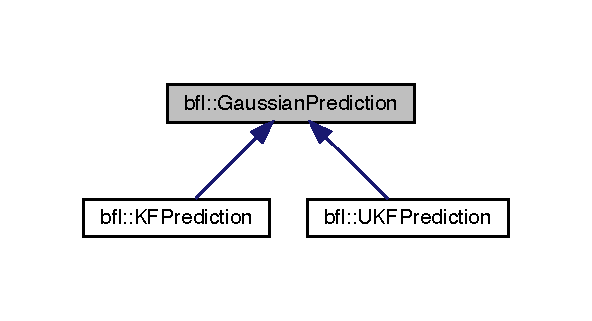
\includegraphics[width=284pt]{classbfl_1_1GaussianPrediction__inherit__graph}
\end{center}
\end{figure}
\subsection*{Public Member Functions}
\begin{DoxyCompactItemize}
\item 
virtual \mbox{\hyperlink{classbfl_1_1GaussianPrediction_a940d6b50429f758b4e085b9b77918a0d}{$\sim$\+Gaussian\+Prediction}} () noexcept
\item 
void \mbox{\hyperlink{classbfl_1_1GaussianPrediction_a37195b6f9a8799ac3d357500b8142676}{predict}} (const \mbox{\hyperlink{classbfl_1_1GaussianMixture}{Gaussian\+Mixture}} \&prev\+\_\+state, \mbox{\hyperlink{classbfl_1_1GaussianMixture}{Gaussian\+Mixture}} \&pred\+\_\+state)
\item 
bool \mbox{\hyperlink{classbfl_1_1GaussianPrediction_ae647821cf920ea81f981ebc9260cdbe6}{skip}} (const std\+::string \&what\+\_\+step, const bool status)
\item 
bool \mbox{\hyperlink{classbfl_1_1GaussianPrediction_a6885530a677199241b2ac11ccdb09688}{get\+Skip\+State}} ()
\item 
bool \mbox{\hyperlink{classbfl_1_1GaussianPrediction_aaf3743111a493b90092b7ead9cbf7825}{get\+Skip\+Exogenous}} ()
\end{DoxyCompactItemize}
\subsection*{Protected Member Functions}
\begin{DoxyCompactItemize}
\item 
\mbox{\hyperlink{classbfl_1_1GaussianPrediction_aacb5ac9c1fdf4e53c84fb681c650c680}{Gaussian\+Prediction}} () noexcept
\item 
\mbox{\hyperlink{classbfl_1_1GaussianPrediction_a8673dfd2a3fbbf84ec99db86f28860e6}{Gaussian\+Prediction}} (\mbox{\hyperlink{classbfl_1_1GaussianPrediction}{Gaussian\+Prediction}} \&\&g\+\_\+prediction) noexcept
\item 
virtual void \mbox{\hyperlink{classbfl_1_1GaussianPrediction_a35e7c490378c9bb48e4becad7fdcb2a1}{predict\+Step}} (const \mbox{\hyperlink{classbfl_1_1GaussianMixture}{Gaussian\+Mixture}} \&prev\+\_\+state, \mbox{\hyperlink{classbfl_1_1GaussianMixture}{Gaussian\+Mixture}} \&pred\+\_\+state)=0
\end{DoxyCompactItemize}
\subsection*{Private Attributes}
\begin{DoxyCompactItemize}
\item 
bool \mbox{\hyperlink{classbfl_1_1GaussianPrediction_a957fc640d2737bf98107ab59b5a4afbf}{skip\+\_\+prediction\+\_\+}} = false
\item 
bool \mbox{\hyperlink{classbfl_1_1GaussianPrediction_a666cc032dab917985809e2851b0af743}{skip\+\_\+state\+\_\+}} = false
\item 
bool \mbox{\hyperlink{classbfl_1_1GaussianPrediction_a15963cb3fce6d30dccc7ca8eb2297573}{skip\+\_\+exogenous\+\_\+}} = false
\end{DoxyCompactItemize}
\subsection*{Friends}
\begin{DoxyCompactItemize}
\item 
class \mbox{\hyperlink{classbfl_1_1GaussianPrediction_a6270a27fe93ac0118907f8cbd64005c8}{Gaussian\+Prediction\+Decorator}}
\item 
class \mbox{\hyperlink{classbfl_1_1GaussianPrediction_a698dcea28e3e0e4b41438a53c8b53a17}{G\+P\+F\+Prediction}}
\end{DoxyCompactItemize}


\subsection{Detailed Description}


Definition at line 13 of file Gaussian\+Prediction.\+h.



\subsection{Constructor \& Destructor Documentation}
\mbox{\Hypertarget{classbfl_1_1GaussianPrediction_a940d6b50429f758b4e085b9b77918a0d}\label{classbfl_1_1GaussianPrediction_a940d6b50429f758b4e085b9b77918a0d}} 
\index{bfl\+::\+Gaussian\+Prediction@{bfl\+::\+Gaussian\+Prediction}!````~Gaussian\+Prediction@{$\sim$\+Gaussian\+Prediction}}
\index{````~Gaussian\+Prediction@{$\sim$\+Gaussian\+Prediction}!bfl\+::\+Gaussian\+Prediction@{bfl\+::\+Gaussian\+Prediction}}
\subsubsection{\texorpdfstring{$\sim$\+Gaussian\+Prediction()}{~GaussianPrediction()}}
{\footnotesize\ttfamily virtual bfl\+::\+Gaussian\+Prediction\+::$\sim$\+Gaussian\+Prediction (\begin{DoxyParamCaption}{ }\end{DoxyParamCaption})\hspace{0.3cm}{\ttfamily [inline]}, {\ttfamily [virtual]}, {\ttfamily [noexcept]}}



Definition at line 16 of file Gaussian\+Prediction.\+h.

\mbox{\Hypertarget{classbfl_1_1GaussianPrediction_aacb5ac9c1fdf4e53c84fb681c650c680}\label{classbfl_1_1GaussianPrediction_aacb5ac9c1fdf4e53c84fb681c650c680}} 
\index{bfl\+::\+Gaussian\+Prediction@{bfl\+::\+Gaussian\+Prediction}!Gaussian\+Prediction@{Gaussian\+Prediction}}
\index{Gaussian\+Prediction@{Gaussian\+Prediction}!bfl\+::\+Gaussian\+Prediction@{bfl\+::\+Gaussian\+Prediction}}
\subsubsection{\texorpdfstring{Gaussian\+Prediction()}{GaussianPrediction()}\hspace{0.1cm}{\footnotesize\ttfamily [1/2]}}
{\footnotesize\ttfamily Gaussian\+Prediction\+::\+Gaussian\+Prediction (\begin{DoxyParamCaption}{ }\end{DoxyParamCaption})\hspace{0.3cm}{\ttfamily [protected]}, {\ttfamily [noexcept]}}



Definition at line 10 of file Gaussian\+Prediction.\+cpp.

\mbox{\Hypertarget{classbfl_1_1GaussianPrediction_a8673dfd2a3fbbf84ec99db86f28860e6}\label{classbfl_1_1GaussianPrediction_a8673dfd2a3fbbf84ec99db86f28860e6}} 
\index{bfl\+::\+Gaussian\+Prediction@{bfl\+::\+Gaussian\+Prediction}!Gaussian\+Prediction@{Gaussian\+Prediction}}
\index{Gaussian\+Prediction@{Gaussian\+Prediction}!bfl\+::\+Gaussian\+Prediction@{bfl\+::\+Gaussian\+Prediction}}
\subsubsection{\texorpdfstring{Gaussian\+Prediction()}{GaussianPrediction()}\hspace{0.1cm}{\footnotesize\ttfamily [2/2]}}
{\footnotesize\ttfamily Gaussian\+Prediction\+::\+Gaussian\+Prediction (\begin{DoxyParamCaption}\item[{\mbox{\hyperlink{classbfl_1_1GaussianPrediction}{Gaussian\+Prediction}} \&\&}]{g\+\_\+prediction }\end{DoxyParamCaption})\hspace{0.3cm}{\ttfamily [protected]}, {\ttfamily [noexcept]}}



Definition at line 13 of file Gaussian\+Prediction.\+cpp.



\subsection{Member Function Documentation}
\mbox{\Hypertarget{classbfl_1_1GaussianPrediction_aaf3743111a493b90092b7ead9cbf7825}\label{classbfl_1_1GaussianPrediction_aaf3743111a493b90092b7ead9cbf7825}} 
\index{bfl\+::\+Gaussian\+Prediction@{bfl\+::\+Gaussian\+Prediction}!get\+Skip\+Exogenous@{get\+Skip\+Exogenous}}
\index{get\+Skip\+Exogenous@{get\+Skip\+Exogenous}!bfl\+::\+Gaussian\+Prediction@{bfl\+::\+Gaussian\+Prediction}}
\subsubsection{\texorpdfstring{get\+Skip\+Exogenous()}{getSkipExogenous()}}
{\footnotesize\ttfamily bool Gaussian\+Prediction\+::get\+Skip\+Exogenous (\begin{DoxyParamCaption}{ }\end{DoxyParamCaption})}



Definition at line 46 of file Gaussian\+Prediction.\+cpp.

\mbox{\Hypertarget{classbfl_1_1GaussianPrediction_a6885530a677199241b2ac11ccdb09688}\label{classbfl_1_1GaussianPrediction_a6885530a677199241b2ac11ccdb09688}} 
\index{bfl\+::\+Gaussian\+Prediction@{bfl\+::\+Gaussian\+Prediction}!get\+Skip\+State@{get\+Skip\+State}}
\index{get\+Skip\+State@{get\+Skip\+State}!bfl\+::\+Gaussian\+Prediction@{bfl\+::\+Gaussian\+Prediction}}
\subsubsection{\texorpdfstring{get\+Skip\+State()}{getSkipState()}}
{\footnotesize\ttfamily bool Gaussian\+Prediction\+::get\+Skip\+State (\begin{DoxyParamCaption}{ }\end{DoxyParamCaption})}



Definition at line 40 of file Gaussian\+Prediction.\+cpp.

\mbox{\Hypertarget{classbfl_1_1GaussianPrediction_a37195b6f9a8799ac3d357500b8142676}\label{classbfl_1_1GaussianPrediction_a37195b6f9a8799ac3d357500b8142676}} 
\index{bfl\+::\+Gaussian\+Prediction@{bfl\+::\+Gaussian\+Prediction}!predict@{predict}}
\index{predict@{predict}!bfl\+::\+Gaussian\+Prediction@{bfl\+::\+Gaussian\+Prediction}}
\subsubsection{\texorpdfstring{predict()}{predict()}}
{\footnotesize\ttfamily void Gaussian\+Prediction\+::predict (\begin{DoxyParamCaption}\item[{const \mbox{\hyperlink{classbfl_1_1GaussianMixture}{Gaussian\+Mixture}} \&}]{prev\+\_\+state,  }\item[{\mbox{\hyperlink{classbfl_1_1GaussianMixture}{Gaussian\+Mixture}} \&}]{pred\+\_\+state }\end{DoxyParamCaption})}



Definition at line 16 of file Gaussian\+Prediction.\+cpp.

\mbox{\Hypertarget{classbfl_1_1GaussianPrediction_a35e7c490378c9bb48e4becad7fdcb2a1}\label{classbfl_1_1GaussianPrediction_a35e7c490378c9bb48e4becad7fdcb2a1}} 
\index{bfl\+::\+Gaussian\+Prediction@{bfl\+::\+Gaussian\+Prediction}!predict\+Step@{predict\+Step}}
\index{predict\+Step@{predict\+Step}!bfl\+::\+Gaussian\+Prediction@{bfl\+::\+Gaussian\+Prediction}}
\subsubsection{\texorpdfstring{predict\+Step()}{predictStep()}}
{\footnotesize\ttfamily virtual void bfl\+::\+Gaussian\+Prediction\+::predict\+Step (\begin{DoxyParamCaption}\item[{const \mbox{\hyperlink{classbfl_1_1GaussianMixture}{Gaussian\+Mixture}} \&}]{prev\+\_\+state,  }\item[{\mbox{\hyperlink{classbfl_1_1GaussianMixture}{Gaussian\+Mixture}} \&}]{pred\+\_\+state }\end{DoxyParamCaption})\hspace{0.3cm}{\ttfamily [protected]}, {\ttfamily [pure virtual]}}



Implemented in \mbox{\hyperlink{classbfl_1_1UKFPrediction_a0ffba56fa1aa4d71c6872e1d76bd2f02}{bfl\+::\+U\+K\+F\+Prediction}}, and \mbox{\hyperlink{classbfl_1_1KFPrediction_aa71d6b8ac030c54e86d3e91a94bb2db9}{bfl\+::\+K\+F\+Prediction}}.

\mbox{\Hypertarget{classbfl_1_1GaussianPrediction_ae647821cf920ea81f981ebc9260cdbe6}\label{classbfl_1_1GaussianPrediction_ae647821cf920ea81f981ebc9260cdbe6}} 
\index{bfl\+::\+Gaussian\+Prediction@{bfl\+::\+Gaussian\+Prediction}!skip@{skip}}
\index{skip@{skip}!bfl\+::\+Gaussian\+Prediction@{bfl\+::\+Gaussian\+Prediction}}
\subsubsection{\texorpdfstring{skip()}{skip()}}
{\footnotesize\ttfamily bool Gaussian\+Prediction\+::skip (\begin{DoxyParamCaption}\item[{const std\+::string \&}]{what\+\_\+step,  }\item[{const bool}]{status }\end{DoxyParamCaption})}



Definition at line 25 of file Gaussian\+Prediction.\+cpp.



\subsection{Friends And Related Function Documentation}
\mbox{\Hypertarget{classbfl_1_1GaussianPrediction_a6270a27fe93ac0118907f8cbd64005c8}\label{classbfl_1_1GaussianPrediction_a6270a27fe93ac0118907f8cbd64005c8}} 
\index{bfl\+::\+Gaussian\+Prediction@{bfl\+::\+Gaussian\+Prediction}!Gaussian\+Prediction\+Decorator@{Gaussian\+Prediction\+Decorator}}
\index{Gaussian\+Prediction\+Decorator@{Gaussian\+Prediction\+Decorator}!bfl\+::\+Gaussian\+Prediction@{bfl\+::\+Gaussian\+Prediction}}
\subsubsection{\texorpdfstring{Gaussian\+Prediction\+Decorator}{GaussianPredictionDecorator}}
{\footnotesize\ttfamily friend class Gaussian\+Prediction\+Decorator\hspace{0.3cm}{\ttfamily [friend]}}



Definition at line 40 of file Gaussian\+Prediction.\+h.

\mbox{\Hypertarget{classbfl_1_1GaussianPrediction_a698dcea28e3e0e4b41438a53c8b53a17}\label{classbfl_1_1GaussianPrediction_a698dcea28e3e0e4b41438a53c8b53a17}} 
\index{bfl\+::\+Gaussian\+Prediction@{bfl\+::\+Gaussian\+Prediction}!G\+P\+F\+Prediction@{G\+P\+F\+Prediction}}
\index{G\+P\+F\+Prediction@{G\+P\+F\+Prediction}!bfl\+::\+Gaussian\+Prediction@{bfl\+::\+Gaussian\+Prediction}}
\subsubsection{\texorpdfstring{G\+P\+F\+Prediction}{GPFPrediction}}
{\footnotesize\ttfamily friend class \mbox{\hyperlink{classbfl_1_1GPFPrediction}{G\+P\+F\+Prediction}}\hspace{0.3cm}{\ttfamily [friend]}}



Definition at line 42 of file Gaussian\+Prediction.\+h.



\subsection{Member Data Documentation}
\mbox{\Hypertarget{classbfl_1_1GaussianPrediction_a15963cb3fce6d30dccc7ca8eb2297573}\label{classbfl_1_1GaussianPrediction_a15963cb3fce6d30dccc7ca8eb2297573}} 
\index{bfl\+::\+Gaussian\+Prediction@{bfl\+::\+Gaussian\+Prediction}!skip\+\_\+exogenous\+\_\+@{skip\+\_\+exogenous\+\_\+}}
\index{skip\+\_\+exogenous\+\_\+@{skip\+\_\+exogenous\+\_\+}!bfl\+::\+Gaussian\+Prediction@{bfl\+::\+Gaussian\+Prediction}}
\subsubsection{\texorpdfstring{skip\+\_\+exogenous\+\_\+}{skip\_exogenous\_}}
{\footnotesize\ttfamily bool bfl\+::\+Gaussian\+Prediction\+::skip\+\_\+exogenous\+\_\+ = false\hspace{0.3cm}{\ttfamily [private]}}



Definition at line 38 of file Gaussian\+Prediction.\+h.

\mbox{\Hypertarget{classbfl_1_1GaussianPrediction_a957fc640d2737bf98107ab59b5a4afbf}\label{classbfl_1_1GaussianPrediction_a957fc640d2737bf98107ab59b5a4afbf}} 
\index{bfl\+::\+Gaussian\+Prediction@{bfl\+::\+Gaussian\+Prediction}!skip\+\_\+prediction\+\_\+@{skip\+\_\+prediction\+\_\+}}
\index{skip\+\_\+prediction\+\_\+@{skip\+\_\+prediction\+\_\+}!bfl\+::\+Gaussian\+Prediction@{bfl\+::\+Gaussian\+Prediction}}
\subsubsection{\texorpdfstring{skip\+\_\+prediction\+\_\+}{skip\_prediction\_}}
{\footnotesize\ttfamily bool bfl\+::\+Gaussian\+Prediction\+::skip\+\_\+prediction\+\_\+ = false\hspace{0.3cm}{\ttfamily [private]}}



Definition at line 34 of file Gaussian\+Prediction.\+h.

\mbox{\Hypertarget{classbfl_1_1GaussianPrediction_a666cc032dab917985809e2851b0af743}\label{classbfl_1_1GaussianPrediction_a666cc032dab917985809e2851b0af743}} 
\index{bfl\+::\+Gaussian\+Prediction@{bfl\+::\+Gaussian\+Prediction}!skip\+\_\+state\+\_\+@{skip\+\_\+state\+\_\+}}
\index{skip\+\_\+state\+\_\+@{skip\+\_\+state\+\_\+}!bfl\+::\+Gaussian\+Prediction@{bfl\+::\+Gaussian\+Prediction}}
\subsubsection{\texorpdfstring{skip\+\_\+state\+\_\+}{skip\_state\_}}
{\footnotesize\ttfamily bool bfl\+::\+Gaussian\+Prediction\+::skip\+\_\+state\+\_\+ = false\hspace{0.3cm}{\ttfamily [private]}}



Definition at line 36 of file Gaussian\+Prediction.\+h.



The documentation for this class was generated from the following files\+:\begin{DoxyCompactItemize}
\item 
/\+Users/\+Claudio/\+Git\+Hub/bayes-\/filters-\/lib/src/\+Bayes\+Filters/include/\+Bayes\+Filters/\mbox{\hyperlink{GaussianPrediction_8h}{Gaussian\+Prediction.\+h}}\item 
/\+Users/\+Claudio/\+Git\+Hub/bayes-\/filters-\/lib/src/\+Bayes\+Filters/src/\mbox{\hyperlink{GaussianPrediction_8cpp}{Gaussian\+Prediction.\+cpp}}\end{DoxyCompactItemize}

\hypertarget{classbfl_1_1GPFCorrection}{}\section{bfl\+:\+:G\+P\+F\+Correction Class Reference}
\label{classbfl_1_1GPFCorrection}\index{bfl\+::\+G\+P\+F\+Correction@{bfl\+::\+G\+P\+F\+Correction}}


{\ttfamily \#include $<$G\+P\+F\+Correction.\+h$>$}



Inheritance diagram for bfl\+:\+:G\+P\+F\+Correction\+:
\nopagebreak
\begin{figure}[H]
\begin{center}
\leavevmode
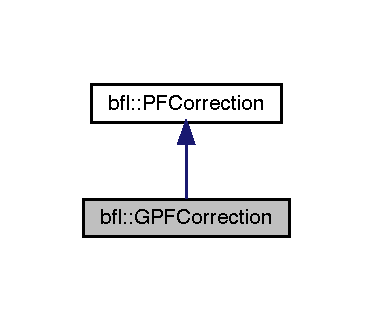
\includegraphics[width=179pt]{classbfl_1_1GPFCorrection__inherit__graph}
\end{center}
\end{figure}
\subsection*{Public Member Functions}
\begin{DoxyCompactItemize}
\item 
\mbox{\hyperlink{classbfl_1_1GPFCorrection_aa3dbc7bc8252895a11fcf547beb231ed}{G\+P\+F\+Correction}} (std\+::unique\+\_\+ptr$<$ \mbox{\hyperlink{classbfl_1_1GaussianCorrection}{bfl\+::\+Gaussian\+Correction}} $>$ gaussian\+\_\+correction, std\+::unique\+\_\+ptr$<$ \mbox{\hyperlink{classbfl_1_1LikelihoodModel}{bfl\+::\+Likelihood\+Model}} $>$ likihood\+\_\+model, std\+::unique\+\_\+ptr$<$ \mbox{\hyperlink{classbfl_1_1StateModel}{bfl\+::\+State\+Model}} $>$ state\+\_\+model) noexcept
\item 
\mbox{\hyperlink{classbfl_1_1GPFCorrection_a92bf53cc6b5890e0f415de3b8f6f0d18}{G\+P\+F\+Correction}} (std\+::unique\+\_\+ptr$<$ \mbox{\hyperlink{classbfl_1_1GaussianCorrection}{bfl\+::\+Gaussian\+Correction}} $>$ gaussian\+\_\+correction, std\+::unique\+\_\+ptr$<$ \mbox{\hyperlink{classbfl_1_1LikelihoodModel}{bfl\+::\+Likelihood\+Model}} $>$ likelihood\+\_\+model, std\+::unique\+\_\+ptr$<$ \mbox{\hyperlink{classbfl_1_1StateModel}{bfl\+::\+State\+Model}} $>$ state\+\_\+model, unsigned int seed) noexcept
\item 
\mbox{\hyperlink{classbfl_1_1GPFCorrection_a7de055f5b25ffe93ab4ff4ca0a6729ee}{G\+P\+F\+Correction}} (\mbox{\hyperlink{classbfl_1_1GPFCorrection}{G\+P\+F\+Correction}} \&\&gpf\+\_\+correction) noexcept
\item 
virtual \mbox{\hyperlink{classbfl_1_1GPFCorrection_abaf42b1e27993b612800d96268a919c9}{$\sim$\+G\+P\+F\+Correction}} () noexcept
\item 
void \mbox{\hyperlink{classbfl_1_1GPFCorrection_a93104fdc7a1bccc4c7350fbd7bd46997}{set\+Likelihood\+Model}} (std\+::unique\+\_\+ptr$<$ \mbox{\hyperlink{classbfl_1_1LikelihoodModel}{bfl\+::\+Likelihood\+Model}} $>$ likelihood\+\_\+model) override
\item 
void \mbox{\hyperlink{classbfl_1_1GPFCorrection_a08ee265b0aed304403a64ef3132ba50a}{set\+Measurement\+Model}} (std\+::unique\+\_\+ptr$<$ \mbox{\hyperlink{classbfl_1_1MeasurementModel}{bfl\+::\+Measurement\+Model}} $>$ measurement\+\_\+model) override
\item 
\mbox{\hyperlink{classbfl_1_1MeasurementModel}{bfl\+::\+Measurement\+Model}} \& \mbox{\hyperlink{classbfl_1_1GPFCorrection_a670298795b61fab434eefd192b7fe81f}{get\+Measurement\+Model}} () override
\item 
\mbox{\hyperlink{classbfl_1_1LikelihoodModel}{bfl\+::\+Likelihood\+Model}} \& \mbox{\hyperlink{classbfl_1_1GPFCorrection_afa1e971c9b618c50bd98f1d5774cff3a}{get\+Likelihood\+Model}} () override
\item 
std\+::pair$<$ bool, Eigen\+::\+Vector\+Xd $>$ \mbox{\hyperlink{classbfl_1_1GPFCorrection_a0df1185be7731e9077eec265b8d6ff8e}{get\+Likelihood}} () override
\item 
void \mbox{\hyperlink{classbfl_1_1PFCorrection_a560666b2e7566a846cb4ce4684e195e0}{correct}} (const \mbox{\hyperlink{classbfl_1_1ParticleSet}{bfl\+::\+Particle\+Set}} \&pred\+\_\+particles, \mbox{\hyperlink{classbfl_1_1ParticleSet}{bfl\+::\+Particle\+Set}} \&cor\+\_\+particles)
\item 
bool \mbox{\hyperlink{classbfl_1_1PFCorrection_ab25e625ea12fe257e0eb85d465835e62}{skip}} (const bool status)
\item 
virtual void \mbox{\hyperlink{classbfl_1_1PFCorrection_aa84e757c694d4ad375cdd543d42ac34c}{set\+Likelihood\+Model}} (std\+::unique\+\_\+ptr$<$ \mbox{\hyperlink{classbfl_1_1LikelihoodModel}{Likelihood\+Model}} $>$ observation\+\_\+model)=0
\item 
virtual void \mbox{\hyperlink{classbfl_1_1PFCorrection_a9844514568f65a0e5fa2cffadea460c6}{set\+Measurement\+Model}} (std\+::unique\+\_\+ptr$<$ \mbox{\hyperlink{classbfl_1_1MeasurementModel}{Measurement\+Model}} $>$ measurement\+\_\+model)=0
\end{DoxyCompactItemize}
\subsection*{Protected Member Functions}
\begin{DoxyCompactItemize}
\item 
void \mbox{\hyperlink{classbfl_1_1GPFCorrection_a291a05d78f7f2ee835140bfe4995a2bb}{correct\+Step}} (const \mbox{\hyperlink{classbfl_1_1ParticleSet}{bfl\+::\+Particle\+Set}} \&pred\+\_\+particles, \mbox{\hyperlink{classbfl_1_1ParticleSet}{bfl\+::\+Particle\+Set}} \&corr\+\_\+particles) override
\item 
Eigen\+::\+Vector\+Xd \mbox{\hyperlink{classbfl_1_1GPFCorrection_a6f8f793f647296a407fbeefbac781908}{sample\+From\+Proposal}} (const Eigen\+::\+Vector\+Xd \&mean, const Eigen\+::\+Matrix\+Xd \&covariance)
\item 
double \mbox{\hyperlink{classbfl_1_1GPFCorrection_a076c8609b08b17fb3c32eaa4e5b7c3eb}{evaluate\+Proposal}} (const Eigen\+::\+Vector\+Xd \&state, const Eigen\+::\+Vector\+Xd \&mean, const Eigen\+::\+Matrix\+Xd \&covariance)
\end{DoxyCompactItemize}
\subsection*{Protected Attributes}
\begin{DoxyCompactItemize}
\item 
std\+::unique\+\_\+ptr$<$ \mbox{\hyperlink{classbfl_1_1GaussianCorrection}{bfl\+::\+Gaussian\+Correction}} $>$ \mbox{\hyperlink{classbfl_1_1GPFCorrection_a43295a0619fa021b6b314c76f046bae8}{gaussian\+\_\+correction\+\_\+}}
\item 
std\+::unique\+\_\+ptr$<$ \mbox{\hyperlink{classbfl_1_1LikelihoodModel}{bfl\+::\+Likelihood\+Model}} $>$ \mbox{\hyperlink{classbfl_1_1GPFCorrection_aabbf55b6addf12146ffd7da12c5475bf}{likelihood\+\_\+model\+\_\+}}
\item 
std\+::unique\+\_\+ptr$<$ \mbox{\hyperlink{classbfl_1_1StateModel}{bfl\+::\+State\+Model}} $>$ \mbox{\hyperlink{classbfl_1_1GPFCorrection_a7b979b09abf016f4e5a0d9f0d5a84917}{state\+\_\+model\+\_\+}}
\begin{DoxyCompactList}\small\item\em The state model is required to evaluate the Markov transition probability that is used in the update of the particles weight. \end{DoxyCompactList}\item 
std\+::mt19937\+\_\+64 \mbox{\hyperlink{classbfl_1_1GPFCorrection_ac1021f6b12969d08231bcefdd0303f80}{generator\+\_\+}}
\item 
std\+::normal\+\_\+distribution$<$ double $>$ \mbox{\hyperlink{classbfl_1_1GPFCorrection_a9d2f1ed3b529e340e5d019d80e572d8d}{distribution\+\_\+}}
\item 
std\+::function$<$ double()$>$ \mbox{\hyperlink{classbfl_1_1GPFCorrection_acec1a6f0c4634b864bc4d22d7f861307}{gaussian\+\_\+random\+\_\+sample\+\_\+}}
\begin{DoxyCompactList}\small\item\em Random number generator function from a Normal distribution. \end{DoxyCompactList}\end{DoxyCompactItemize}


\subsection{Detailed Description}


Definition at line 20 of file G\+P\+F\+Correction.\+h.



\subsection{Constructor \& Destructor Documentation}
\mbox{\Hypertarget{classbfl_1_1GPFCorrection_aa3dbc7bc8252895a11fcf547beb231ed}\label{classbfl_1_1GPFCorrection_aa3dbc7bc8252895a11fcf547beb231ed}} 
\index{bfl\+::\+G\+P\+F\+Correction@{bfl\+::\+G\+P\+F\+Correction}!G\+P\+F\+Correction@{G\+P\+F\+Correction}}
\index{G\+P\+F\+Correction@{G\+P\+F\+Correction}!bfl\+::\+G\+P\+F\+Correction@{bfl\+::\+G\+P\+F\+Correction}}
\subsubsection{\texorpdfstring{G\+P\+F\+Correction()}{GPFCorrection()}\hspace{0.1cm}{\footnotesize\ttfamily [1/3]}}
{\footnotesize\ttfamily bfl\+::\+G\+P\+F\+Correction\+::\+G\+P\+F\+Correction (\begin{DoxyParamCaption}\item[{std\+::unique\+\_\+ptr$<$ \mbox{\hyperlink{classbfl_1_1GaussianCorrection}{bfl\+::\+Gaussian\+Correction}} $>$}]{gaussian\+\_\+correction,  }\item[{std\+::unique\+\_\+ptr$<$ \mbox{\hyperlink{classbfl_1_1LikelihoodModel}{bfl\+::\+Likelihood\+Model}} $>$}]{likihood\+\_\+model,  }\item[{std\+::unique\+\_\+ptr$<$ \mbox{\hyperlink{classbfl_1_1StateModel}{bfl\+::\+State\+Model}} $>$}]{state\+\_\+model }\end{DoxyParamCaption})\hspace{0.3cm}{\ttfamily [noexcept]}}

\mbox{\Hypertarget{classbfl_1_1GPFCorrection_a92bf53cc6b5890e0f415de3b8f6f0d18}\label{classbfl_1_1GPFCorrection_a92bf53cc6b5890e0f415de3b8f6f0d18}} 
\index{bfl\+::\+G\+P\+F\+Correction@{bfl\+::\+G\+P\+F\+Correction}!G\+P\+F\+Correction@{G\+P\+F\+Correction}}
\index{G\+P\+F\+Correction@{G\+P\+F\+Correction}!bfl\+::\+G\+P\+F\+Correction@{bfl\+::\+G\+P\+F\+Correction}}
\subsubsection{\texorpdfstring{G\+P\+F\+Correction()}{GPFCorrection()}\hspace{0.1cm}{\footnotesize\ttfamily [2/3]}}
{\footnotesize\ttfamily bfl\+::\+G\+P\+F\+Correction\+::\+G\+P\+F\+Correction (\begin{DoxyParamCaption}\item[{std\+::unique\+\_\+ptr$<$ \mbox{\hyperlink{classbfl_1_1GaussianCorrection}{bfl\+::\+Gaussian\+Correction}} $>$}]{gaussian\+\_\+correction,  }\item[{std\+::unique\+\_\+ptr$<$ \mbox{\hyperlink{classbfl_1_1LikelihoodModel}{bfl\+::\+Likelihood\+Model}} $>$}]{likelihood\+\_\+model,  }\item[{std\+::unique\+\_\+ptr$<$ \mbox{\hyperlink{classbfl_1_1StateModel}{bfl\+::\+State\+Model}} $>$}]{state\+\_\+model,  }\item[{unsigned int}]{seed }\end{DoxyParamCaption})\hspace{0.3cm}{\ttfamily [noexcept]}}

\mbox{\Hypertarget{classbfl_1_1GPFCorrection_a7de055f5b25ffe93ab4ff4ca0a6729ee}\label{classbfl_1_1GPFCorrection_a7de055f5b25ffe93ab4ff4ca0a6729ee}} 
\index{bfl\+::\+G\+P\+F\+Correction@{bfl\+::\+G\+P\+F\+Correction}!G\+P\+F\+Correction@{G\+P\+F\+Correction}}
\index{G\+P\+F\+Correction@{G\+P\+F\+Correction}!bfl\+::\+G\+P\+F\+Correction@{bfl\+::\+G\+P\+F\+Correction}}
\subsubsection{\texorpdfstring{G\+P\+F\+Correction()}{GPFCorrection()}\hspace{0.1cm}{\footnotesize\ttfamily [3/3]}}
{\footnotesize\ttfamily G\+P\+F\+Correction\+::\+G\+P\+F\+Correction (\begin{DoxyParamCaption}\item[{\mbox{\hyperlink{classbfl_1_1GPFCorrection}{G\+P\+F\+Correction}} \&\&}]{gpf\+\_\+correction }\end{DoxyParamCaption})\hspace{0.3cm}{\ttfamily [noexcept]}}



Definition at line 37 of file G\+P\+F\+Correction.\+cpp.

\mbox{\Hypertarget{classbfl_1_1GPFCorrection_abaf42b1e27993b612800d96268a919c9}\label{classbfl_1_1GPFCorrection_abaf42b1e27993b612800d96268a919c9}} 
\index{bfl\+::\+G\+P\+F\+Correction@{bfl\+::\+G\+P\+F\+Correction}!````~G\+P\+F\+Correction@{$\sim$\+G\+P\+F\+Correction}}
\index{````~G\+P\+F\+Correction@{$\sim$\+G\+P\+F\+Correction}!bfl\+::\+G\+P\+F\+Correction@{bfl\+::\+G\+P\+F\+Correction}}
\subsubsection{\texorpdfstring{$\sim$\+G\+P\+F\+Correction()}{~GPFCorrection()}}
{\footnotesize\ttfamily virtual bfl\+::\+G\+P\+F\+Correction\+::$\sim$\+G\+P\+F\+Correction (\begin{DoxyParamCaption}{ }\end{DoxyParamCaption})\hspace{0.3cm}{\ttfamily [inline]}, {\ttfamily [virtual]}, {\ttfamily [noexcept]}}



Definition at line 29 of file G\+P\+F\+Correction.\+h.



\subsection{Member Function Documentation}
\mbox{\Hypertarget{classbfl_1_1PFCorrection_a560666b2e7566a846cb4ce4684e195e0}\label{classbfl_1_1PFCorrection_a560666b2e7566a846cb4ce4684e195e0}} 
\index{bfl\+::\+G\+P\+F\+Correction@{bfl\+::\+G\+P\+F\+Correction}!correct@{correct}}
\index{correct@{correct}!bfl\+::\+G\+P\+F\+Correction@{bfl\+::\+G\+P\+F\+Correction}}
\subsubsection{\texorpdfstring{correct()}{correct()}}
{\footnotesize\ttfamily void P\+F\+Correction\+::correct (\begin{DoxyParamCaption}\item[{const \mbox{\hyperlink{classbfl_1_1ParticleSet}{bfl\+::\+Particle\+Set}} \&}]{pred\+\_\+particles,  }\item[{\mbox{\hyperlink{classbfl_1_1ParticleSet}{bfl\+::\+Particle\+Set}} \&}]{cor\+\_\+particles }\end{DoxyParamCaption})\hspace{0.3cm}{\ttfamily [inherited]}}



Definition at line 10 of file P\+F\+Correction.\+cpp.

\mbox{\Hypertarget{classbfl_1_1GPFCorrection_a291a05d78f7f2ee835140bfe4995a2bb}\label{classbfl_1_1GPFCorrection_a291a05d78f7f2ee835140bfe4995a2bb}} 
\index{bfl\+::\+G\+P\+F\+Correction@{bfl\+::\+G\+P\+F\+Correction}!correct\+Step@{correct\+Step}}
\index{correct\+Step@{correct\+Step}!bfl\+::\+G\+P\+F\+Correction@{bfl\+::\+G\+P\+F\+Correction}}
\subsubsection{\texorpdfstring{correct\+Step()}{correctStep()}}
{\footnotesize\ttfamily void G\+P\+F\+Correction\+::correct\+Step (\begin{DoxyParamCaption}\item[{const \mbox{\hyperlink{classbfl_1_1ParticleSet}{bfl\+::\+Particle\+Set}} \&}]{pred\+\_\+particles,  }\item[{\mbox{\hyperlink{classbfl_1_1ParticleSet}{bfl\+::\+Particle\+Set}} \&}]{corr\+\_\+particles }\end{DoxyParamCaption})\hspace{0.3cm}{\ttfamily [override]}, {\ttfamily [protected]}, {\ttfamily [virtual]}}



Implements \mbox{\hyperlink{classbfl_1_1PFCorrection_ae0413156a1258d88485e57a983c89af1}{bfl\+::\+P\+F\+Correction}}.



Definition at line 77 of file G\+P\+F\+Correction.\+cpp.



References bfl\+::\+Gaussian\+Mixture\+::components, bfl\+::\+Gaussian\+Mixture\+::covariance(), bfl\+::\+Gaussian\+Mixture\+::mean(), bfl\+::\+Particle\+Set\+::state(), and bfl\+::\+Gaussian\+Mixture\+::weight().

Here is the call graph for this function\+:
\nopagebreak
\begin{figure}[H]
\begin{center}
\leavevmode
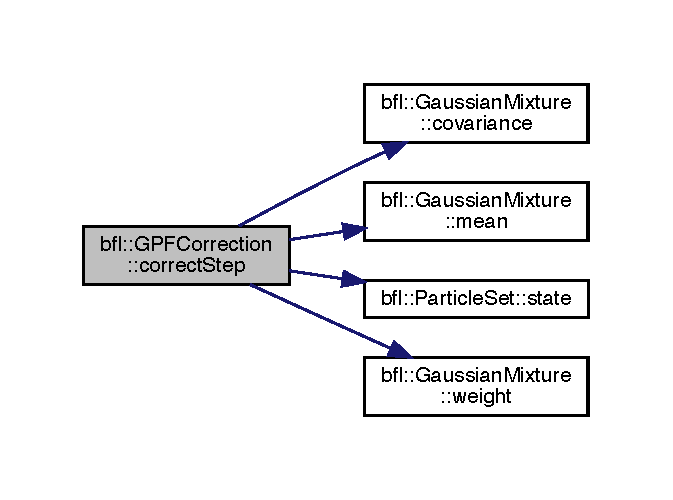
\includegraphics[width=323pt]{classbfl_1_1GPFCorrection_a291a05d78f7f2ee835140bfe4995a2bb_cgraph}
\end{center}
\end{figure}
\mbox{\Hypertarget{classbfl_1_1GPFCorrection_a076c8609b08b17fb3c32eaa4e5b7c3eb}\label{classbfl_1_1GPFCorrection_a076c8609b08b17fb3c32eaa4e5b7c3eb}} 
\index{bfl\+::\+G\+P\+F\+Correction@{bfl\+::\+G\+P\+F\+Correction}!evaluate\+Proposal@{evaluate\+Proposal}}
\index{evaluate\+Proposal@{evaluate\+Proposal}!bfl\+::\+G\+P\+F\+Correction@{bfl\+::\+G\+P\+F\+Correction}}
\subsubsection{\texorpdfstring{evaluate\+Proposal()}{evaluateProposal()}}
{\footnotesize\ttfamily double G\+P\+F\+Correction\+::evaluate\+Proposal (\begin{DoxyParamCaption}\item[{const Eigen\+::\+Vector\+Xd \&}]{state,  }\item[{const Eigen\+::\+Vector\+Xd \&}]{mean,  }\item[{const Eigen\+::\+Matrix\+Xd \&}]{covariance }\end{DoxyParamCaption})\hspace{0.3cm}{\ttfamily [protected]}}



Definition at line 133 of file G\+P\+F\+Correction.\+cpp.

\mbox{\Hypertarget{classbfl_1_1GPFCorrection_a0df1185be7731e9077eec265b8d6ff8e}\label{classbfl_1_1GPFCorrection_a0df1185be7731e9077eec265b8d6ff8e}} 
\index{bfl\+::\+G\+P\+F\+Correction@{bfl\+::\+G\+P\+F\+Correction}!get\+Likelihood@{get\+Likelihood}}
\index{get\+Likelihood@{get\+Likelihood}!bfl\+::\+G\+P\+F\+Correction@{bfl\+::\+G\+P\+F\+Correction}}
\subsubsection{\texorpdfstring{get\+Likelihood()}{getLikelihood()}}
{\footnotesize\ttfamily std\+::pair$<$ bool, Eigen\+::\+Vector\+Xd $>$ G\+P\+F\+Correction\+::get\+Likelihood (\begin{DoxyParamCaption}{ }\end{DoxyParamCaption})\hspace{0.3cm}{\ttfamily [override]}, {\ttfamily [virtual]}}



Implements \mbox{\hyperlink{classbfl_1_1PFCorrection_ab6eca766077c4ab1db3417dab6c44d27}{bfl\+::\+P\+F\+Correction}}.



Definition at line 71 of file G\+P\+F\+Correction.\+cpp.

\mbox{\Hypertarget{classbfl_1_1GPFCorrection_afa1e971c9b618c50bd98f1d5774cff3a}\label{classbfl_1_1GPFCorrection_afa1e971c9b618c50bd98f1d5774cff3a}} 
\index{bfl\+::\+G\+P\+F\+Correction@{bfl\+::\+G\+P\+F\+Correction}!get\+Likelihood\+Model@{get\+Likelihood\+Model}}
\index{get\+Likelihood\+Model@{get\+Likelihood\+Model}!bfl\+::\+G\+P\+F\+Correction@{bfl\+::\+G\+P\+F\+Correction}}
\subsubsection{\texorpdfstring{get\+Likelihood\+Model()}{getLikelihoodModel()}}
{\footnotesize\ttfamily \mbox{\hyperlink{classbfl_1_1LikelihoodModel}{Likelihood\+Model}} \& G\+P\+F\+Correction\+::get\+Likelihood\+Model (\begin{DoxyParamCaption}{ }\end{DoxyParamCaption})\hspace{0.3cm}{\ttfamily [override]}, {\ttfamily [virtual]}}



Implements \mbox{\hyperlink{classbfl_1_1PFCorrection_ad812d0b488e0882b246dd19d4f6818e1}{bfl\+::\+P\+F\+Correction}}.



Definition at line 65 of file G\+P\+F\+Correction.\+cpp.

\mbox{\Hypertarget{classbfl_1_1GPFCorrection_a670298795b61fab434eefd192b7fe81f}\label{classbfl_1_1GPFCorrection_a670298795b61fab434eefd192b7fe81f}} 
\index{bfl\+::\+G\+P\+F\+Correction@{bfl\+::\+G\+P\+F\+Correction}!get\+Measurement\+Model@{get\+Measurement\+Model}}
\index{get\+Measurement\+Model@{get\+Measurement\+Model}!bfl\+::\+G\+P\+F\+Correction@{bfl\+::\+G\+P\+F\+Correction}}
\subsubsection{\texorpdfstring{get\+Measurement\+Model()}{getMeasurementModel()}}
{\footnotesize\ttfamily \mbox{\hyperlink{classbfl_1_1MeasurementModel}{Measurement\+Model}} \& G\+P\+F\+Correction\+::get\+Measurement\+Model (\begin{DoxyParamCaption}{ }\end{DoxyParamCaption})\hspace{0.3cm}{\ttfamily [override]}, {\ttfamily [virtual]}}



Implements \mbox{\hyperlink{classbfl_1_1PFCorrection_a891c7d498caffb4d11e5ebdaa475c683}{bfl\+::\+P\+F\+Correction}}.



Definition at line 59 of file G\+P\+F\+Correction.\+cpp.

\mbox{\Hypertarget{classbfl_1_1GPFCorrection_a6f8f793f647296a407fbeefbac781908}\label{classbfl_1_1GPFCorrection_a6f8f793f647296a407fbeefbac781908}} 
\index{bfl\+::\+G\+P\+F\+Correction@{bfl\+::\+G\+P\+F\+Correction}!sample\+From\+Proposal@{sample\+From\+Proposal}}
\index{sample\+From\+Proposal@{sample\+From\+Proposal}!bfl\+::\+G\+P\+F\+Correction@{bfl\+::\+G\+P\+F\+Correction}}
\subsubsection{\texorpdfstring{sample\+From\+Proposal()}{sampleFromProposal()}}
{\footnotesize\ttfamily Eigen\+::\+Vector\+Xd G\+P\+F\+Correction\+::sample\+From\+Proposal (\begin{DoxyParamCaption}\item[{const Eigen\+::\+Vector\+Xd \&}]{mean,  }\item[{const Eigen\+::\+Matrix\+Xd \&}]{covariance }\end{DoxyParamCaption})\hspace{0.3cm}{\ttfamily [protected]}}



Definition at line 113 of file G\+P\+F\+Correction.\+cpp.

\mbox{\Hypertarget{classbfl_1_1PFCorrection_aa84e757c694d4ad375cdd543d42ac34c}\label{classbfl_1_1PFCorrection_aa84e757c694d4ad375cdd543d42ac34c}} 
\index{bfl\+::\+G\+P\+F\+Correction@{bfl\+::\+G\+P\+F\+Correction}!set\+Likelihood\+Model@{set\+Likelihood\+Model}}
\index{set\+Likelihood\+Model@{set\+Likelihood\+Model}!bfl\+::\+G\+P\+F\+Correction@{bfl\+::\+G\+P\+F\+Correction}}
\subsubsection{\texorpdfstring{set\+Likelihood\+Model()}{setLikelihoodModel()}\hspace{0.1cm}{\footnotesize\ttfamily [1/2]}}
{\footnotesize\ttfamily virtual void bfl\+::\+P\+F\+Correction\+::set\+Likelihood\+Model (\begin{DoxyParamCaption}\item[{std\+::unique\+\_\+ptr$<$ \mbox{\hyperlink{classbfl_1_1LikelihoodModel}{Likelihood\+Model}} $>$}]{observation\+\_\+model }\end{DoxyParamCaption})\hspace{0.3cm}{\ttfamily [pure virtual]}, {\ttfamily [inherited]}}



Implemented in \mbox{\hyperlink{classbfl_1_1BoostrapCorrection_a75d770c17ac4142833c926e9e6dc32db}{bfl\+::\+Boostrap\+Correction}}, and \mbox{\hyperlink{classbfl_1_1PFCorrectionDecorator_ab1065f8e47e4e51bc846b2d693b4bb88}{bfl\+::\+P\+F\+Correction\+Decorator}}.

\mbox{\Hypertarget{classbfl_1_1GPFCorrection_a93104fdc7a1bccc4c7350fbd7bd46997}\label{classbfl_1_1GPFCorrection_a93104fdc7a1bccc4c7350fbd7bd46997}} 
\index{bfl\+::\+G\+P\+F\+Correction@{bfl\+::\+G\+P\+F\+Correction}!set\+Likelihood\+Model@{set\+Likelihood\+Model}}
\index{set\+Likelihood\+Model@{set\+Likelihood\+Model}!bfl\+::\+G\+P\+F\+Correction@{bfl\+::\+G\+P\+F\+Correction}}
\subsubsection{\texorpdfstring{set\+Likelihood\+Model()}{setLikelihoodModel()}\hspace{0.1cm}{\footnotesize\ttfamily [2/2]}}
{\footnotesize\ttfamily void G\+P\+F\+Correction\+::set\+Likelihood\+Model (\begin{DoxyParamCaption}\item[{std\+::unique\+\_\+ptr$<$ \mbox{\hyperlink{classbfl_1_1LikelihoodModel}{bfl\+::\+Likelihood\+Model}} $>$}]{likelihood\+\_\+model }\end{DoxyParamCaption})\hspace{0.3cm}{\ttfamily [override]}}



Definition at line 47 of file G\+P\+F\+Correction.\+cpp.

\mbox{\Hypertarget{classbfl_1_1PFCorrection_a9844514568f65a0e5fa2cffadea460c6}\label{classbfl_1_1PFCorrection_a9844514568f65a0e5fa2cffadea460c6}} 
\index{bfl\+::\+G\+P\+F\+Correction@{bfl\+::\+G\+P\+F\+Correction}!set\+Measurement\+Model@{set\+Measurement\+Model}}
\index{set\+Measurement\+Model@{set\+Measurement\+Model}!bfl\+::\+G\+P\+F\+Correction@{bfl\+::\+G\+P\+F\+Correction}}
\subsubsection{\texorpdfstring{set\+Measurement\+Model()}{setMeasurementModel()}\hspace{0.1cm}{\footnotesize\ttfamily [1/2]}}
{\footnotesize\ttfamily virtual void bfl\+::\+P\+F\+Correction\+::set\+Measurement\+Model (\begin{DoxyParamCaption}\item[{std\+::unique\+\_\+ptr$<$ \mbox{\hyperlink{classbfl_1_1MeasurementModel}{Measurement\+Model}} $>$}]{measurement\+\_\+model }\end{DoxyParamCaption})\hspace{0.3cm}{\ttfamily [pure virtual]}, {\ttfamily [inherited]}}



Implemented in \mbox{\hyperlink{classbfl_1_1BoostrapCorrection_af6e02e5d6e6426cbee2825a77c79da43}{bfl\+::\+Boostrap\+Correction}}, and \mbox{\hyperlink{classbfl_1_1PFCorrectionDecorator_a6e96dbb6591e44d9ebaa186c6e50569b}{bfl\+::\+P\+F\+Correction\+Decorator}}.

\mbox{\Hypertarget{classbfl_1_1GPFCorrection_a08ee265b0aed304403a64ef3132ba50a}\label{classbfl_1_1GPFCorrection_a08ee265b0aed304403a64ef3132ba50a}} 
\index{bfl\+::\+G\+P\+F\+Correction@{bfl\+::\+G\+P\+F\+Correction}!set\+Measurement\+Model@{set\+Measurement\+Model}}
\index{set\+Measurement\+Model@{set\+Measurement\+Model}!bfl\+::\+G\+P\+F\+Correction@{bfl\+::\+G\+P\+F\+Correction}}
\subsubsection{\texorpdfstring{set\+Measurement\+Model()}{setMeasurementModel()}\hspace{0.1cm}{\footnotesize\ttfamily [2/2]}}
{\footnotesize\ttfamily void G\+P\+F\+Correction\+::set\+Measurement\+Model (\begin{DoxyParamCaption}\item[{std\+::unique\+\_\+ptr$<$ \mbox{\hyperlink{classbfl_1_1MeasurementModel}{bfl\+::\+Measurement\+Model}} $>$}]{measurement\+\_\+model }\end{DoxyParamCaption})\hspace{0.3cm}{\ttfamily [override]}}



Definition at line 53 of file G\+P\+F\+Correction.\+cpp.

\mbox{\Hypertarget{classbfl_1_1PFCorrection_ab25e625ea12fe257e0eb85d465835e62}\label{classbfl_1_1PFCorrection_ab25e625ea12fe257e0eb85d465835e62}} 
\index{bfl\+::\+G\+P\+F\+Correction@{bfl\+::\+G\+P\+F\+Correction}!skip@{skip}}
\index{skip@{skip}!bfl\+::\+G\+P\+F\+Correction@{bfl\+::\+G\+P\+F\+Correction}}
\subsubsection{\texorpdfstring{skip()}{skip()}}
{\footnotesize\ttfamily bool P\+F\+Correction\+::skip (\begin{DoxyParamCaption}\item[{const bool}]{status }\end{DoxyParamCaption})\hspace{0.3cm}{\ttfamily [inherited]}}



Definition at line 20 of file P\+F\+Correction.\+cpp.



\subsection{Member Data Documentation}
\mbox{\Hypertarget{classbfl_1_1GPFCorrection_a9d2f1ed3b529e340e5d019d80e572d8d}\label{classbfl_1_1GPFCorrection_a9d2f1ed3b529e340e5d019d80e572d8d}} 
\index{bfl\+::\+G\+P\+F\+Correction@{bfl\+::\+G\+P\+F\+Correction}!distribution\+\_\+@{distribution\+\_\+}}
\index{distribution\+\_\+@{distribution\+\_\+}!bfl\+::\+G\+P\+F\+Correction@{bfl\+::\+G\+P\+F\+Correction}}
\subsubsection{\texorpdfstring{distribution\+\_\+}{distribution\_}}
{\footnotesize\ttfamily std\+::normal\+\_\+distribution$<$double$>$ bfl\+::\+G\+P\+F\+Correction\+::distribution\+\_\+\hspace{0.3cm}{\ttfamily [protected]}}



Definition at line 60 of file G\+P\+F\+Correction.\+h.

\mbox{\Hypertarget{classbfl_1_1GPFCorrection_a43295a0619fa021b6b314c76f046bae8}\label{classbfl_1_1GPFCorrection_a43295a0619fa021b6b314c76f046bae8}} 
\index{bfl\+::\+G\+P\+F\+Correction@{bfl\+::\+G\+P\+F\+Correction}!gaussian\+\_\+correction\+\_\+@{gaussian\+\_\+correction\+\_\+}}
\index{gaussian\+\_\+correction\+\_\+@{gaussian\+\_\+correction\+\_\+}!bfl\+::\+G\+P\+F\+Correction@{bfl\+::\+G\+P\+F\+Correction}}
\subsubsection{\texorpdfstring{gaussian\+\_\+correction\+\_\+}{gaussian\_correction\_}}
{\footnotesize\ttfamily std\+::unique\+\_\+ptr$<$\mbox{\hyperlink{classbfl_1_1GaussianCorrection}{bfl\+::\+Gaussian\+Correction}}$>$ bfl\+::\+G\+P\+F\+Correction\+::gaussian\+\_\+correction\+\_\+\hspace{0.3cm}{\ttfamily [protected]}}



Definition at line 48 of file G\+P\+F\+Correction.\+h.

\mbox{\Hypertarget{classbfl_1_1GPFCorrection_acec1a6f0c4634b864bc4d22d7f861307}\label{classbfl_1_1GPFCorrection_acec1a6f0c4634b864bc4d22d7f861307}} 
\index{bfl\+::\+G\+P\+F\+Correction@{bfl\+::\+G\+P\+F\+Correction}!gaussian\+\_\+random\+\_\+sample\+\_\+@{gaussian\+\_\+random\+\_\+sample\+\_\+}}
\index{gaussian\+\_\+random\+\_\+sample\+\_\+@{gaussian\+\_\+random\+\_\+sample\+\_\+}!bfl\+::\+G\+P\+F\+Correction@{bfl\+::\+G\+P\+F\+Correction}}
\subsubsection{\texorpdfstring{gaussian\+\_\+random\+\_\+sample\+\_\+}{gaussian\_random\_sample\_}}
{\footnotesize\ttfamily std\+::function$<$double()$>$ bfl\+::\+G\+P\+F\+Correction\+::gaussian\+\_\+random\+\_\+sample\+\_\+\hspace{0.3cm}{\ttfamily [protected]}}



Random number generator function from a Normal distribution. 

A call to {\ttfamily \mbox{\hyperlink{classbfl_1_1GPFCorrection_acec1a6f0c4634b864bc4d22d7f861307}{gaussian\+\_\+random\+\_\+sample\+\_\+()}}} returns a double-\/precision floating-\/point random number. 

Definition at line 66 of file G\+P\+F\+Correction.\+h.

\mbox{\Hypertarget{classbfl_1_1GPFCorrection_ac1021f6b12969d08231bcefdd0303f80}\label{classbfl_1_1GPFCorrection_ac1021f6b12969d08231bcefdd0303f80}} 
\index{bfl\+::\+G\+P\+F\+Correction@{bfl\+::\+G\+P\+F\+Correction}!generator\+\_\+@{generator\+\_\+}}
\index{generator\+\_\+@{generator\+\_\+}!bfl\+::\+G\+P\+F\+Correction@{bfl\+::\+G\+P\+F\+Correction}}
\subsubsection{\texorpdfstring{generator\+\_\+}{generator\_}}
{\footnotesize\ttfamily std\+::mt19937\+\_\+64 bfl\+::\+G\+P\+F\+Correction\+::generator\+\_\+\hspace{0.3cm}{\ttfamily [protected]}}



Definition at line 58 of file G\+P\+F\+Correction.\+h.

\mbox{\Hypertarget{classbfl_1_1GPFCorrection_aabbf55b6addf12146ffd7da12c5475bf}\label{classbfl_1_1GPFCorrection_aabbf55b6addf12146ffd7da12c5475bf}} 
\index{bfl\+::\+G\+P\+F\+Correction@{bfl\+::\+G\+P\+F\+Correction}!likelihood\+\_\+model\+\_\+@{likelihood\+\_\+model\+\_\+}}
\index{likelihood\+\_\+model\+\_\+@{likelihood\+\_\+model\+\_\+}!bfl\+::\+G\+P\+F\+Correction@{bfl\+::\+G\+P\+F\+Correction}}
\subsubsection{\texorpdfstring{likelihood\+\_\+model\+\_\+}{likelihood\_model\_}}
{\footnotesize\ttfamily std\+::unique\+\_\+ptr$<$\mbox{\hyperlink{classbfl_1_1LikelihoodModel}{bfl\+::\+Likelihood\+Model}}$>$ bfl\+::\+G\+P\+F\+Correction\+::likelihood\+\_\+model\+\_\+\hspace{0.3cm}{\ttfamily [protected]}}



Definition at line 50 of file G\+P\+F\+Correction.\+h.

\mbox{\Hypertarget{classbfl_1_1GPFCorrection_a7b979b09abf016f4e5a0d9f0d5a84917}\label{classbfl_1_1GPFCorrection_a7b979b09abf016f4e5a0d9f0d5a84917}} 
\index{bfl\+::\+G\+P\+F\+Correction@{bfl\+::\+G\+P\+F\+Correction}!state\+\_\+model\+\_\+@{state\+\_\+model\+\_\+}}
\index{state\+\_\+model\+\_\+@{state\+\_\+model\+\_\+}!bfl\+::\+G\+P\+F\+Correction@{bfl\+::\+G\+P\+F\+Correction}}
\subsubsection{\texorpdfstring{state\+\_\+model\+\_\+}{state\_model\_}}
{\footnotesize\ttfamily std\+::unique\+\_\+ptr$<$\mbox{\hyperlink{classbfl_1_1StateModel}{bfl\+::\+State\+Model}}$>$ bfl\+::\+G\+P\+F\+Correction\+::state\+\_\+model\+\_\+\hspace{0.3cm}{\ttfamily [protected]}}



The state model is required to evaluate the Markov transition probability that is used in the update of the particles weight. 



Definition at line 56 of file G\+P\+F\+Correction.\+h.



The documentation for this class was generated from the following files\+:\begin{DoxyCompactItemize}
\item 
/\+Users/\+Claudio/\+Git\+Hub/bayes-\/filters-\/lib/src/\+Bayes\+Filters/include/\+Bayes\+Filters/\mbox{\hyperlink{GPFCorrection_8h}{G\+P\+F\+Correction.\+h}}\item 
/\+Users/\+Claudio/\+Git\+Hub/bayes-\/filters-\/lib/src/\+Bayes\+Filters/src/\mbox{\hyperlink{GPFCorrection_8cpp}{G\+P\+F\+Correction.\+cpp}}\end{DoxyCompactItemize}

\hypertarget{classbfl_1_1GPFPrediction}{}\section{bfl\+:\+:G\+P\+F\+Prediction Class Reference}
\label{classbfl_1_1GPFPrediction}\index{bfl\+::\+G\+P\+F\+Prediction@{bfl\+::\+G\+P\+F\+Prediction}}


{\ttfamily \#include $<$G\+P\+F\+Prediction.\+h$>$}



Inheritance diagram for bfl\+:\+:G\+P\+F\+Prediction\+:
\nopagebreak
\begin{figure}[H]
\begin{center}
\leavevmode
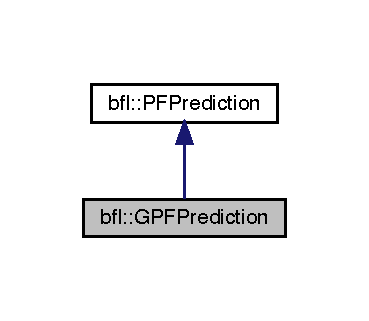
\includegraphics[width=177pt]{classbfl_1_1GPFPrediction__inherit__graph}
\end{center}
\end{figure}
\subsection*{Public Member Functions}
\begin{DoxyCompactItemize}
\item 
\mbox{\hyperlink{classbfl_1_1GPFPrediction_a03ed76dc8f4dd587389b1a3c200c8c6f}{G\+P\+F\+Prediction}} (std\+::unique\+\_\+ptr$<$ \mbox{\hyperlink{classbfl_1_1GaussianPrediction}{bfl\+::\+Gaussian\+Prediction}} $>$ gauss\+\_\+pred) noexcept
\item 
\mbox{\hyperlink{classbfl_1_1GPFPrediction_a4dffe9e873409370675450840fe93236}{G\+P\+F\+Prediction}} (\mbox{\hyperlink{classbfl_1_1GPFPrediction}{G\+P\+F\+Prediction}} \&\&gpf\+\_\+prediction) noexcept
\item 
virtual \mbox{\hyperlink{classbfl_1_1GPFPrediction_a9758eba10d2b369b20912ff47bcf937b}{$\sim$\+G\+P\+F\+Prediction}} () noexcept
\item 
void \mbox{\hyperlink{classbfl_1_1GPFPrediction_a29d7a4777cb8007a356b98e66db28f53}{set\+State\+Model}} (std\+::unique\+\_\+ptr$<$ \mbox{\hyperlink{classbfl_1_1StateModel}{bfl\+::\+State\+Model}} $>$ state\+\_\+model) override
\item 
\mbox{\hyperlink{classbfl_1_1StateModel}{bfl\+::\+State\+Model}} \& \mbox{\hyperlink{classbfl_1_1GPFPrediction_a3b8c347633b8db630af4945548980794}{get\+State\+Model}} () override
\item 
void \mbox{\hyperlink{classbfl_1_1PFPrediction_a129dcd1cccd2da9827ef0c49c90b9345}{predict}} (const \mbox{\hyperlink{classbfl_1_1ParticleSet}{bfl\+::\+Particle\+Set}} \&prev\+\_\+particles, \mbox{\hyperlink{classbfl_1_1ParticleSet}{bfl\+::\+Particle\+Set}} \&pred\+\_\+particles)
\item 
bool \mbox{\hyperlink{classbfl_1_1PFPrediction_a364cc35a151e5298c4024d681f3e04d9}{skip}} (const std\+::string \&what\+\_\+step, const bool status)
\item 
bool \mbox{\hyperlink{classbfl_1_1PFPrediction_a323ca5612dd7ad924fd448a629359ad2}{get\+Skip\+State}} ()
\item 
bool \mbox{\hyperlink{classbfl_1_1PFPrediction_a432b8e84dbf00432158aa82312386d63}{get\+Skip\+Exogenous}} ()
\item 
virtual void \mbox{\hyperlink{classbfl_1_1PFPrediction_ac39683650d7f89c59f1426dd7743354e}{set\+State\+Model}} (std\+::unique\+\_\+ptr$<$ \mbox{\hyperlink{classbfl_1_1StateModel}{State\+Model}} $>$ state\+\_\+model)=0
\item 
virtual void \mbox{\hyperlink{classbfl_1_1PFPrediction_ada843698204584e97d4ff6728c8e8264}{set\+Exogenous\+Model}} (std\+::unique\+\_\+ptr$<$ \mbox{\hyperlink{classbfl_1_1ExogenousModel}{Exogenous\+Model}} $>$ exogenous\+\_\+model)
\item 
virtual \mbox{\hyperlink{classbfl_1_1ExogenousModel}{Exogenous\+Model}} \& \mbox{\hyperlink{classbfl_1_1PFPrediction_aefa127a440649447e8ac659ef65b7a2a}{get\+Exogenous\+Model}} ()
\end{DoxyCompactItemize}
\subsection*{Protected Member Functions}
\begin{DoxyCompactItemize}
\item 
void \mbox{\hyperlink{classbfl_1_1GPFPrediction_a9eca49102486401afeff748c37438ca3}{predict\+Step}} (const \mbox{\hyperlink{classbfl_1_1ParticleSet}{bfl\+::\+Particle\+Set}} \&previous\+\_\+particles, \mbox{\hyperlink{classbfl_1_1ParticleSet}{bfl\+::\+Particle\+Set}} \&predicted\+\_\+particles) override
\end{DoxyCompactItemize}
\subsection*{Protected Attributes}
\begin{DoxyCompactItemize}
\item 
std\+::unique\+\_\+ptr$<$ \mbox{\hyperlink{classbfl_1_1GaussianPrediction}{bfl\+::\+Gaussian\+Prediction}} $>$ \mbox{\hyperlink{classbfl_1_1GPFPrediction_a2cd16a1045d72c56bbfac5d20d965a03}{gaussian\+\_\+prediction\+\_\+}}
\end{DoxyCompactItemize}


\subsection{Detailed Description}


Definition at line 17 of file G\+P\+F\+Prediction.\+h.



\subsection{Constructor \& Destructor Documentation}
\mbox{\Hypertarget{classbfl_1_1GPFPrediction_a03ed76dc8f4dd587389b1a3c200c8c6f}\label{classbfl_1_1GPFPrediction_a03ed76dc8f4dd587389b1a3c200c8c6f}} 
\index{bfl\+::\+G\+P\+F\+Prediction@{bfl\+::\+G\+P\+F\+Prediction}!G\+P\+F\+Prediction@{G\+P\+F\+Prediction}}
\index{G\+P\+F\+Prediction@{G\+P\+F\+Prediction}!bfl\+::\+G\+P\+F\+Prediction@{bfl\+::\+G\+P\+F\+Prediction}}
\subsubsection{\texorpdfstring{G\+P\+F\+Prediction()}{GPFPrediction()}\hspace{0.1cm}{\footnotesize\ttfamily [1/2]}}
{\footnotesize\ttfamily bfl\+::\+G\+P\+F\+Prediction\+::\+G\+P\+F\+Prediction (\begin{DoxyParamCaption}\item[{std\+::unique\+\_\+ptr$<$ \mbox{\hyperlink{classbfl_1_1GaussianPrediction}{bfl\+::\+Gaussian\+Prediction}} $>$}]{gauss\+\_\+pred }\end{DoxyParamCaption})\hspace{0.3cm}{\ttfamily [noexcept]}}

\mbox{\Hypertarget{classbfl_1_1GPFPrediction_a4dffe9e873409370675450840fe93236}\label{classbfl_1_1GPFPrediction_a4dffe9e873409370675450840fe93236}} 
\index{bfl\+::\+G\+P\+F\+Prediction@{bfl\+::\+G\+P\+F\+Prediction}!G\+P\+F\+Prediction@{G\+P\+F\+Prediction}}
\index{G\+P\+F\+Prediction@{G\+P\+F\+Prediction}!bfl\+::\+G\+P\+F\+Prediction@{bfl\+::\+G\+P\+F\+Prediction}}
\subsubsection{\texorpdfstring{G\+P\+F\+Prediction()}{GPFPrediction()}\hspace{0.1cm}{\footnotesize\ttfamily [2/2]}}
{\footnotesize\ttfamily G\+P\+F\+Prediction\+::\+G\+P\+F\+Prediction (\begin{DoxyParamCaption}\item[{\mbox{\hyperlink{classbfl_1_1GPFPrediction}{G\+P\+F\+Prediction}} \&\&}]{gpf\+\_\+prediction }\end{DoxyParamCaption})\hspace{0.3cm}{\ttfamily [noexcept]}}



Definition at line 13 of file G\+P\+F\+Prediction.\+cpp.

\mbox{\Hypertarget{classbfl_1_1GPFPrediction_a9758eba10d2b369b20912ff47bcf937b}\label{classbfl_1_1GPFPrediction_a9758eba10d2b369b20912ff47bcf937b}} 
\index{bfl\+::\+G\+P\+F\+Prediction@{bfl\+::\+G\+P\+F\+Prediction}!````~G\+P\+F\+Prediction@{$\sim$\+G\+P\+F\+Prediction}}
\index{````~G\+P\+F\+Prediction@{$\sim$\+G\+P\+F\+Prediction}!bfl\+::\+G\+P\+F\+Prediction@{bfl\+::\+G\+P\+F\+Prediction}}
\subsubsection{\texorpdfstring{$\sim$\+G\+P\+F\+Prediction()}{~GPFPrediction()}}
{\footnotesize\ttfamily virtual bfl\+::\+G\+P\+F\+Prediction\+::$\sim$\+G\+P\+F\+Prediction (\begin{DoxyParamCaption}{ }\end{DoxyParamCaption})\hspace{0.3cm}{\ttfamily [inline]}, {\ttfamily [virtual]}, {\ttfamily [noexcept]}}



Definition at line 24 of file G\+P\+F\+Prediction.\+h.



\subsection{Member Function Documentation}
\mbox{\Hypertarget{classbfl_1_1PFPrediction_aefa127a440649447e8ac659ef65b7a2a}\label{classbfl_1_1PFPrediction_aefa127a440649447e8ac659ef65b7a2a}} 
\index{bfl\+::\+G\+P\+F\+Prediction@{bfl\+::\+G\+P\+F\+Prediction}!get\+Exogenous\+Model@{get\+Exogenous\+Model}}
\index{get\+Exogenous\+Model@{get\+Exogenous\+Model}!bfl\+::\+G\+P\+F\+Prediction@{bfl\+::\+G\+P\+F\+Prediction}}
\subsubsection{\texorpdfstring{get\+Exogenous\+Model()}{getExogenousModel()}}
{\footnotesize\ttfamily \mbox{\hyperlink{classbfl_1_1ExogenousModel}{Exogenous\+Model}} \& P\+F\+Prediction\+::get\+Exogenous\+Model (\begin{DoxyParamCaption}{ }\end{DoxyParamCaption})\hspace{0.3cm}{\ttfamily [virtual]}, {\ttfamily [inherited]}}



Reimplemented in \mbox{\hyperlink{classbfl_1_1PFPredictionDecorator_a8d25d3765f642f7de1af897d088d8da9}{bfl\+::\+P\+F\+Prediction\+Decorator}}.



Definition at line 60 of file P\+F\+Prediction.\+cpp.

\mbox{\Hypertarget{classbfl_1_1PFPrediction_a432b8e84dbf00432158aa82312386d63}\label{classbfl_1_1PFPrediction_a432b8e84dbf00432158aa82312386d63}} 
\index{bfl\+::\+G\+P\+F\+Prediction@{bfl\+::\+G\+P\+F\+Prediction}!get\+Skip\+Exogenous@{get\+Skip\+Exogenous}}
\index{get\+Skip\+Exogenous@{get\+Skip\+Exogenous}!bfl\+::\+G\+P\+F\+Prediction@{bfl\+::\+G\+P\+F\+Prediction}}
\subsubsection{\texorpdfstring{get\+Skip\+Exogenous()}{getSkipExogenous()}}
{\footnotesize\ttfamily bool P\+F\+Prediction\+::get\+Skip\+Exogenous (\begin{DoxyParamCaption}{ }\end{DoxyParamCaption})\hspace{0.3cm}{\ttfamily [inherited]}}



Definition at line 54 of file P\+F\+Prediction.\+cpp.

\mbox{\Hypertarget{classbfl_1_1PFPrediction_a323ca5612dd7ad924fd448a629359ad2}\label{classbfl_1_1PFPrediction_a323ca5612dd7ad924fd448a629359ad2}} 
\index{bfl\+::\+G\+P\+F\+Prediction@{bfl\+::\+G\+P\+F\+Prediction}!get\+Skip\+State@{get\+Skip\+State}}
\index{get\+Skip\+State@{get\+Skip\+State}!bfl\+::\+G\+P\+F\+Prediction@{bfl\+::\+G\+P\+F\+Prediction}}
\subsubsection{\texorpdfstring{get\+Skip\+State()}{getSkipState()}}
{\footnotesize\ttfamily bool P\+F\+Prediction\+::get\+Skip\+State (\begin{DoxyParamCaption}{ }\end{DoxyParamCaption})\hspace{0.3cm}{\ttfamily [inherited]}}



Definition at line 48 of file P\+F\+Prediction.\+cpp.

\mbox{\Hypertarget{classbfl_1_1GPFPrediction_a3b8c347633b8db630af4945548980794}\label{classbfl_1_1GPFPrediction_a3b8c347633b8db630af4945548980794}} 
\index{bfl\+::\+G\+P\+F\+Prediction@{bfl\+::\+G\+P\+F\+Prediction}!get\+State\+Model@{get\+State\+Model}}
\index{get\+State\+Model@{get\+State\+Model}!bfl\+::\+G\+P\+F\+Prediction@{bfl\+::\+G\+P\+F\+Prediction}}
\subsubsection{\texorpdfstring{get\+State\+Model()}{getStateModel()}}
{\footnotesize\ttfamily \mbox{\hyperlink{classbfl_1_1StateModel}{State\+Model}} \& G\+P\+F\+Prediction\+::get\+State\+Model (\begin{DoxyParamCaption}{ }\end{DoxyParamCaption})\hspace{0.3cm}{\ttfamily [override]}, {\ttfamily [virtual]}}



Implements \mbox{\hyperlink{classbfl_1_1PFPrediction_a1a0f7a1d66a6849c2de10459c6b8f8ac}{bfl\+::\+P\+F\+Prediction}}.



Definition at line 18 of file G\+P\+F\+Prediction.\+cpp.

\mbox{\Hypertarget{classbfl_1_1PFPrediction_a129dcd1cccd2da9827ef0c49c90b9345}\label{classbfl_1_1PFPrediction_a129dcd1cccd2da9827ef0c49c90b9345}} 
\index{bfl\+::\+G\+P\+F\+Prediction@{bfl\+::\+G\+P\+F\+Prediction}!predict@{predict}}
\index{predict@{predict}!bfl\+::\+G\+P\+F\+Prediction@{bfl\+::\+G\+P\+F\+Prediction}}
\subsubsection{\texorpdfstring{predict()}{predict()}}
{\footnotesize\ttfamily void P\+F\+Prediction\+::predict (\begin{DoxyParamCaption}\item[{const \mbox{\hyperlink{classbfl_1_1ParticleSet}{bfl\+::\+Particle\+Set}} \&}]{prev\+\_\+particles,  }\item[{\mbox{\hyperlink{classbfl_1_1ParticleSet}{bfl\+::\+Particle\+Set}} \&}]{pred\+\_\+particles }\end{DoxyParamCaption})\hspace{0.3cm}{\ttfamily [inherited]}}



Definition at line 24 of file P\+F\+Prediction.\+cpp.

\mbox{\Hypertarget{classbfl_1_1GPFPrediction_a9eca49102486401afeff748c37438ca3}\label{classbfl_1_1GPFPrediction_a9eca49102486401afeff748c37438ca3}} 
\index{bfl\+::\+G\+P\+F\+Prediction@{bfl\+::\+G\+P\+F\+Prediction}!predict\+Step@{predict\+Step}}
\index{predict\+Step@{predict\+Step}!bfl\+::\+G\+P\+F\+Prediction@{bfl\+::\+G\+P\+F\+Prediction}}
\subsubsection{\texorpdfstring{predict\+Step()}{predictStep()}}
{\footnotesize\ttfamily void G\+P\+F\+Prediction\+::predict\+Step (\begin{DoxyParamCaption}\item[{const \mbox{\hyperlink{classbfl_1_1ParticleSet}{bfl\+::\+Particle\+Set}} \&}]{previous\+\_\+particles,  }\item[{\mbox{\hyperlink{classbfl_1_1ParticleSet}{bfl\+::\+Particle\+Set}} \&}]{predicted\+\_\+particles }\end{DoxyParamCaption})\hspace{0.3cm}{\ttfamily [override]}, {\ttfamily [protected]}, {\ttfamily [virtual]}}



Implements \mbox{\hyperlink{classbfl_1_1PFPrediction_ade49953e2beed6d12f9716254ccbba71}{bfl\+::\+P\+F\+Prediction}}.



Definition at line 30 of file G\+P\+F\+Prediction.\+cpp.



References bfl\+::\+Particle\+Set\+::state(), and bfl\+::\+Gaussian\+Mixture\+::weight().

Here is the call graph for this function\+:
\nopagebreak
\begin{figure}[H]
\begin{center}
\leavevmode
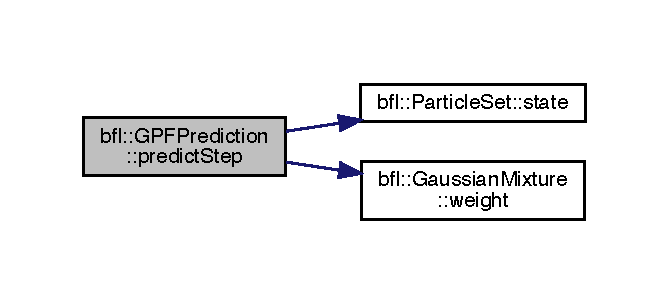
\includegraphics[width=321pt]{classbfl_1_1GPFPrediction_a9eca49102486401afeff748c37438ca3_cgraph}
\end{center}
\end{figure}
\mbox{\Hypertarget{classbfl_1_1PFPrediction_ada843698204584e97d4ff6728c8e8264}\label{classbfl_1_1PFPrediction_ada843698204584e97d4ff6728c8e8264}} 
\index{bfl\+::\+G\+P\+F\+Prediction@{bfl\+::\+G\+P\+F\+Prediction}!set\+Exogenous\+Model@{set\+Exogenous\+Model}}
\index{set\+Exogenous\+Model@{set\+Exogenous\+Model}!bfl\+::\+G\+P\+F\+Prediction@{bfl\+::\+G\+P\+F\+Prediction}}
\subsubsection{\texorpdfstring{set\+Exogenous\+Model()}{setExogenousModel()}}
{\footnotesize\ttfamily void P\+F\+Prediction\+::set\+Exogenous\+Model (\begin{DoxyParamCaption}\item[{std\+::unique\+\_\+ptr$<$ \mbox{\hyperlink{classbfl_1_1ExogenousModel}{Exogenous\+Model}} $>$}]{exogenous\+\_\+model }\end{DoxyParamCaption})\hspace{0.3cm}{\ttfamily [virtual]}, {\ttfamily [inherited]}}



Reimplemented in \mbox{\hyperlink{classbfl_1_1PFPredictionDecorator_a3c38ae386456ecd0fd1b609b381395ec}{bfl\+::\+P\+F\+Prediction\+Decorator}}.



Definition at line 66 of file P\+F\+Prediction.\+cpp.

\mbox{\Hypertarget{classbfl_1_1GPFPrediction_a29d7a4777cb8007a356b98e66db28f53}\label{classbfl_1_1GPFPrediction_a29d7a4777cb8007a356b98e66db28f53}} 
\index{bfl\+::\+G\+P\+F\+Prediction@{bfl\+::\+G\+P\+F\+Prediction}!set\+State\+Model@{set\+State\+Model}}
\index{set\+State\+Model@{set\+State\+Model}!bfl\+::\+G\+P\+F\+Prediction@{bfl\+::\+G\+P\+F\+Prediction}}
\subsubsection{\texorpdfstring{set\+State\+Model()}{setStateModel()}\hspace{0.1cm}{\footnotesize\ttfamily [1/2]}}
{\footnotesize\ttfamily void G\+P\+F\+Prediction\+::set\+State\+Model (\begin{DoxyParamCaption}\item[{std\+::unique\+\_\+ptr$<$ \mbox{\hyperlink{classbfl_1_1StateModel}{bfl\+::\+State\+Model}} $>$}]{state\+\_\+model }\end{DoxyParamCaption})\hspace{0.3cm}{\ttfamily [override]}}



Definition at line 24 of file G\+P\+F\+Prediction.\+cpp.

\mbox{\Hypertarget{classbfl_1_1PFPrediction_ac39683650d7f89c59f1426dd7743354e}\label{classbfl_1_1PFPrediction_ac39683650d7f89c59f1426dd7743354e}} 
\index{bfl\+::\+G\+P\+F\+Prediction@{bfl\+::\+G\+P\+F\+Prediction}!set\+State\+Model@{set\+State\+Model}}
\index{set\+State\+Model@{set\+State\+Model}!bfl\+::\+G\+P\+F\+Prediction@{bfl\+::\+G\+P\+F\+Prediction}}
\subsubsection{\texorpdfstring{set\+State\+Model()}{setStateModel()}\hspace{0.1cm}{\footnotesize\ttfamily [2/2]}}
{\footnotesize\ttfamily virtual void bfl\+::\+P\+F\+Prediction\+::set\+State\+Model (\begin{DoxyParamCaption}\item[{std\+::unique\+\_\+ptr$<$ \mbox{\hyperlink{classbfl_1_1StateModel}{State\+Model}} $>$}]{state\+\_\+model }\end{DoxyParamCaption})\hspace{0.3cm}{\ttfamily [pure virtual]}, {\ttfamily [inherited]}}



Implemented in \mbox{\hyperlink{classbfl_1_1PFPredictionDecorator_ad269dfbdecf19d67717a8bc44f0bd286}{bfl\+::\+P\+F\+Prediction\+Decorator}}, and \mbox{\hyperlink{classbfl_1_1DrawParticles_acb607ab90c22a43a72a75576acb898a4}{bfl\+::\+Draw\+Particles}}.

\mbox{\Hypertarget{classbfl_1_1PFPrediction_a364cc35a151e5298c4024d681f3e04d9}\label{classbfl_1_1PFPrediction_a364cc35a151e5298c4024d681f3e04d9}} 
\index{bfl\+::\+G\+P\+F\+Prediction@{bfl\+::\+G\+P\+F\+Prediction}!skip@{skip}}
\index{skip@{skip}!bfl\+::\+G\+P\+F\+Prediction@{bfl\+::\+G\+P\+F\+Prediction}}
\subsubsection{\texorpdfstring{skip()}{skip()}}
{\footnotesize\ttfamily bool P\+F\+Prediction\+::skip (\begin{DoxyParamCaption}\item[{const std\+::string \&}]{what\+\_\+step,  }\item[{const bool}]{status }\end{DoxyParamCaption})\hspace{0.3cm}{\ttfamily [inherited]}}



Definition at line 33 of file P\+F\+Prediction.\+cpp.



\subsection{Member Data Documentation}
\mbox{\Hypertarget{classbfl_1_1GPFPrediction_a2cd16a1045d72c56bbfac5d20d965a03}\label{classbfl_1_1GPFPrediction_a2cd16a1045d72c56bbfac5d20d965a03}} 
\index{bfl\+::\+G\+P\+F\+Prediction@{bfl\+::\+G\+P\+F\+Prediction}!gaussian\+\_\+prediction\+\_\+@{gaussian\+\_\+prediction\+\_\+}}
\index{gaussian\+\_\+prediction\+\_\+@{gaussian\+\_\+prediction\+\_\+}!bfl\+::\+G\+P\+F\+Prediction@{bfl\+::\+G\+P\+F\+Prediction}}
\subsubsection{\texorpdfstring{gaussian\+\_\+prediction\+\_\+}{gaussian\_prediction\_}}
{\footnotesize\ttfamily std\+::unique\+\_\+ptr$<$\mbox{\hyperlink{classbfl_1_1GaussianPrediction}{bfl\+::\+Gaussian\+Prediction}}$>$ bfl\+::\+G\+P\+F\+Prediction\+::gaussian\+\_\+prediction\+\_\+\hspace{0.3cm}{\ttfamily [protected]}}



Definition at line 33 of file G\+P\+F\+Prediction.\+h.



The documentation for this class was generated from the following files\+:\begin{DoxyCompactItemize}
\item 
/\+Users/\+Claudio/\+Git\+Hub/bayes-\/filters-\/lib/src/\+Bayes\+Filters/include/\+Bayes\+Filters/\mbox{\hyperlink{GPFPrediction_8h}{G\+P\+F\+Prediction.\+h}}\item 
/\+Users/\+Claudio/\+Git\+Hub/bayes-\/filters-\/lib/src/\+Bayes\+Filters/src/\mbox{\hyperlink{GPFPrediction_8cpp}{G\+P\+F\+Prediction.\+cpp}}\end{DoxyCompactItemize}

\hypertarget{classbfl_1_1HistoryBuffer}{}\section{bfl\+:\+:History\+Buffer Class Reference}
\label{classbfl_1_1HistoryBuffer}\index{bfl\+::\+History\+Buffer@{bfl\+::\+History\+Buffer}}


{\ttfamily \#include $<$History\+Buffer.\+h$>$}

\subsection*{Public Member Functions}
\begin{DoxyCompactItemize}
\item 
\mbox{\hyperlink{classbfl_1_1HistoryBuffer_a0b0c850ed4a50eeb7eb3d88e10937c1b}{History\+Buffer}} () noexcept
\item 
\mbox{\hyperlink{classbfl_1_1HistoryBuffer_ab88b9511d782060c1b3b0952f608cb08}{History\+Buffer}} (\mbox{\hyperlink{classbfl_1_1HistoryBuffer}{History\+Buffer}} \&\&history\+\_\+buffer) noexcept
\item 
\mbox{\hyperlink{classbfl_1_1HistoryBuffer}{History\+Buffer}} \& \mbox{\hyperlink{classbfl_1_1HistoryBuffer_a77a0d57c5413a374bf21d51693a81715}{operator=}} (\mbox{\hyperlink{classbfl_1_1HistoryBuffer}{History\+Buffer}} \&\&history\+\_\+buffer) noexcept
\item 
\mbox{\hyperlink{classbfl_1_1HistoryBuffer_af61bc43a22241a71223dbc1223480d90}{$\sim$\+History\+Buffer}} () noexcept
\item 
void \mbox{\hyperlink{classbfl_1_1HistoryBuffer_ae48829f91c14283fe403f34461c7e359}{add\+Element}} (const Eigen\+::\+Ref$<$ const Eigen\+::\+Vector\+Xd $>$ \&element)
\item 
Eigen\+::\+Matrix\+Xd \mbox{\hyperlink{classbfl_1_1HistoryBuffer_a30d73c7a82d817122a4b5329e6b042e4}{get\+History\+Buffer}} () const
\item 
bool \mbox{\hyperlink{classbfl_1_1HistoryBuffer_a34bc31abe55f9d43575919a15a1f90c3}{set\+History\+Size}} (const unsigned int window)
\item 
unsigned int \mbox{\hyperlink{classbfl_1_1HistoryBuffer_a0fef292d6e577b8f2f7d2035927edddb}{get\+History\+Size}} () const
\item 
bool \mbox{\hyperlink{classbfl_1_1HistoryBuffer_a3113fb73683eb5001e7fef0c6d3806cb}{decrease\+History\+Size}} ()
\item 
bool \mbox{\hyperlink{classbfl_1_1HistoryBuffer_a495d4786a46ffe6da00179f412d44f93}{increase\+History\+Size}} ()
\item 
bool \mbox{\hyperlink{classbfl_1_1HistoryBuffer_ad9d3d44d796dccc5adb22be9594618c8}{clear}} ()
\end{DoxyCompactItemize}
\subsection*{Private Attributes}
\begin{DoxyCompactItemize}
\item 
unsigned int \mbox{\hyperlink{classbfl_1_1HistoryBuffer_a135dd1829747ba2f414f12fd8282f75a}{window\+\_\+}} = 5
\item 
const unsigned int \mbox{\hyperlink{classbfl_1_1HistoryBuffer_aeb4d2b9c58f06177b0daaf640e2b6c9e}{max\+\_\+window\+\_\+}} = 30
\item 
std\+::deque$<$ Eigen\+::\+Vector\+Xd $>$ \mbox{\hyperlink{classbfl_1_1HistoryBuffer_a31dcf97b1b7fc9e97b8dd4774e24e4d7}{history\+\_\+buffer\+\_\+}}
\end{DoxyCompactItemize}


\subsection{Detailed Description}


Definition at line 13 of file History\+Buffer.\+h.



\subsection{Constructor \& Destructor Documentation}
\mbox{\Hypertarget{classbfl_1_1HistoryBuffer_a0b0c850ed4a50eeb7eb3d88e10937c1b}\label{classbfl_1_1HistoryBuffer_a0b0c850ed4a50eeb7eb3d88e10937c1b}} 
\index{bfl\+::\+History\+Buffer@{bfl\+::\+History\+Buffer}!History\+Buffer@{History\+Buffer}}
\index{History\+Buffer@{History\+Buffer}!bfl\+::\+History\+Buffer@{bfl\+::\+History\+Buffer}}
\subsubsection{\texorpdfstring{History\+Buffer()}{HistoryBuffer()}\hspace{0.1cm}{\footnotesize\ttfamily [1/2]}}
{\footnotesize\ttfamily bfl\+::\+History\+Buffer\+::\+History\+Buffer (\begin{DoxyParamCaption}{ }\end{DoxyParamCaption})\hspace{0.3cm}{\ttfamily [inline]}, {\ttfamily [noexcept]}}



Definition at line 16 of file History\+Buffer.\+h.

\mbox{\Hypertarget{classbfl_1_1HistoryBuffer_ab88b9511d782060c1b3b0952f608cb08}\label{classbfl_1_1HistoryBuffer_ab88b9511d782060c1b3b0952f608cb08}} 
\index{bfl\+::\+History\+Buffer@{bfl\+::\+History\+Buffer}!History\+Buffer@{History\+Buffer}}
\index{History\+Buffer@{History\+Buffer}!bfl\+::\+History\+Buffer@{bfl\+::\+History\+Buffer}}
\subsubsection{\texorpdfstring{History\+Buffer()}{HistoryBuffer()}\hspace{0.1cm}{\footnotesize\ttfamily [2/2]}}
{\footnotesize\ttfamily History\+Buffer\+::\+History\+Buffer (\begin{DoxyParamCaption}\item[{\mbox{\hyperlink{classbfl_1_1HistoryBuffer}{History\+Buffer}} \&\&}]{history\+\_\+buffer }\end{DoxyParamCaption})\hspace{0.3cm}{\ttfamily [noexcept]}}



Definition at line 7 of file History\+Buffer.\+cpp.

\mbox{\Hypertarget{classbfl_1_1HistoryBuffer_af61bc43a22241a71223dbc1223480d90}\label{classbfl_1_1HistoryBuffer_af61bc43a22241a71223dbc1223480d90}} 
\index{bfl\+::\+History\+Buffer@{bfl\+::\+History\+Buffer}!````~History\+Buffer@{$\sim$\+History\+Buffer}}
\index{````~History\+Buffer@{$\sim$\+History\+Buffer}!bfl\+::\+History\+Buffer@{bfl\+::\+History\+Buffer}}
\subsubsection{\texorpdfstring{$\sim$\+History\+Buffer()}{~HistoryBuffer()}}
{\footnotesize\ttfamily bfl\+::\+History\+Buffer\+::$\sim$\+History\+Buffer (\begin{DoxyParamCaption}{ }\end{DoxyParamCaption})\hspace{0.3cm}{\ttfamily [inline]}, {\ttfamily [noexcept]}}



Definition at line 22 of file History\+Buffer.\+h.



\subsection{Member Function Documentation}
\mbox{\Hypertarget{classbfl_1_1HistoryBuffer_ae48829f91c14283fe403f34461c7e359}\label{classbfl_1_1HistoryBuffer_ae48829f91c14283fe403f34461c7e359}} 
\index{bfl\+::\+History\+Buffer@{bfl\+::\+History\+Buffer}!add\+Element@{add\+Element}}
\index{add\+Element@{add\+Element}!bfl\+::\+History\+Buffer@{bfl\+::\+History\+Buffer}}
\subsubsection{\texorpdfstring{add\+Element()}{addElement()}}
{\footnotesize\ttfamily void History\+Buffer\+::add\+Element (\begin{DoxyParamCaption}\item[{const Eigen\+::\+Ref$<$ const Eigen\+::\+Vector\+Xd $>$ \&}]{element }\end{DoxyParamCaption})}



Definition at line 29 of file History\+Buffer.\+cpp.

\mbox{\Hypertarget{classbfl_1_1HistoryBuffer_ad9d3d44d796dccc5adb22be9594618c8}\label{classbfl_1_1HistoryBuffer_ad9d3d44d796dccc5adb22be9594618c8}} 
\index{bfl\+::\+History\+Buffer@{bfl\+::\+History\+Buffer}!clear@{clear}}
\index{clear@{clear}!bfl\+::\+History\+Buffer@{bfl\+::\+History\+Buffer}}
\subsubsection{\texorpdfstring{clear()}{clear()}}
{\footnotesize\ttfamily bool History\+Buffer\+::clear (\begin{DoxyParamCaption}{ }\end{DoxyParamCaption})}



Definition at line 82 of file History\+Buffer.\+cpp.

\mbox{\Hypertarget{classbfl_1_1HistoryBuffer_a3113fb73683eb5001e7fef0c6d3806cb}\label{classbfl_1_1HistoryBuffer_a3113fb73683eb5001e7fef0c6d3806cb}} 
\index{bfl\+::\+History\+Buffer@{bfl\+::\+History\+Buffer}!decrease\+History\+Size@{decrease\+History\+Size}}
\index{decrease\+History\+Size@{decrease\+History\+Size}!bfl\+::\+History\+Buffer@{bfl\+::\+History\+Buffer}}
\subsubsection{\texorpdfstring{decrease\+History\+Size()}{decreaseHistorySize()}}
{\footnotesize\ttfamily bool History\+Buffer\+::decrease\+History\+Size (\begin{DoxyParamCaption}{ }\end{DoxyParamCaption})}



Definition at line 70 of file History\+Buffer.\+cpp.

\mbox{\Hypertarget{classbfl_1_1HistoryBuffer_a30d73c7a82d817122a4b5329e6b042e4}\label{classbfl_1_1HistoryBuffer_a30d73c7a82d817122a4b5329e6b042e4}} 
\index{bfl\+::\+History\+Buffer@{bfl\+::\+History\+Buffer}!get\+History\+Buffer@{get\+History\+Buffer}}
\index{get\+History\+Buffer@{get\+History\+Buffer}!bfl\+::\+History\+Buffer@{bfl\+::\+History\+Buffer}}
\subsubsection{\texorpdfstring{get\+History\+Buffer()}{getHistoryBuffer()}}
{\footnotesize\ttfamily Matrix\+Xd History\+Buffer\+::get\+History\+Buffer (\begin{DoxyParamCaption}{ }\end{DoxyParamCaption}) const}



Definition at line 38 of file History\+Buffer.\+cpp.

\mbox{\Hypertarget{classbfl_1_1HistoryBuffer_a0fef292d6e577b8f2f7d2035927edddb}\label{classbfl_1_1HistoryBuffer_a0fef292d6e577b8f2f7d2035927edddb}} 
\index{bfl\+::\+History\+Buffer@{bfl\+::\+History\+Buffer}!get\+History\+Size@{get\+History\+Size}}
\index{get\+History\+Size@{get\+History\+Size}!bfl\+::\+History\+Buffer@{bfl\+::\+History\+Buffer}}
\subsubsection{\texorpdfstring{get\+History\+Size()}{getHistorySize()}}
{\footnotesize\ttfamily unsigned int bfl\+::\+History\+Buffer\+::get\+History\+Size (\begin{DoxyParamCaption}{ }\end{DoxyParamCaption}) const\hspace{0.3cm}{\ttfamily [inline]}}



Definition at line 30 of file History\+Buffer.\+h.



References window\+\_\+.

\mbox{\Hypertarget{classbfl_1_1HistoryBuffer_a495d4786a46ffe6da00179f412d44f93}\label{classbfl_1_1HistoryBuffer_a495d4786a46ffe6da00179f412d44f93}} 
\index{bfl\+::\+History\+Buffer@{bfl\+::\+History\+Buffer}!increase\+History\+Size@{increase\+History\+Size}}
\index{increase\+History\+Size@{increase\+History\+Size}!bfl\+::\+History\+Buffer@{bfl\+::\+History\+Buffer}}
\subsubsection{\texorpdfstring{increase\+History\+Size()}{increaseHistorySize()}}
{\footnotesize\ttfamily bool History\+Buffer\+::increase\+History\+Size (\begin{DoxyParamCaption}{ }\end{DoxyParamCaption})}



Definition at line 76 of file History\+Buffer.\+cpp.

\mbox{\Hypertarget{classbfl_1_1HistoryBuffer_a77a0d57c5413a374bf21d51693a81715}\label{classbfl_1_1HistoryBuffer_a77a0d57c5413a374bf21d51693a81715}} 
\index{bfl\+::\+History\+Buffer@{bfl\+::\+History\+Buffer}!operator=@{operator=}}
\index{operator=@{operator=}!bfl\+::\+History\+Buffer@{bfl\+::\+History\+Buffer}}
\subsubsection{\texorpdfstring{operator=()}{operator=()}}
{\footnotesize\ttfamily \mbox{\hyperlink{classbfl_1_1HistoryBuffer}{History\+Buffer}} \& History\+Buffer\+::operator= (\begin{DoxyParamCaption}\item[{\mbox{\hyperlink{classbfl_1_1HistoryBuffer}{History\+Buffer}} \&\&}]{history\+\_\+buffer }\end{DoxyParamCaption})\hspace{0.3cm}{\ttfamily [noexcept]}}



Definition at line 15 of file History\+Buffer.\+cpp.



References window\+\_\+.

\mbox{\Hypertarget{classbfl_1_1HistoryBuffer_a34bc31abe55f9d43575919a15a1f90c3}\label{classbfl_1_1HistoryBuffer_a34bc31abe55f9d43575919a15a1f90c3}} 
\index{bfl\+::\+History\+Buffer@{bfl\+::\+History\+Buffer}!set\+History\+Size@{set\+History\+Size}}
\index{set\+History\+Size@{set\+History\+Size}!bfl\+::\+History\+Buffer@{bfl\+::\+History\+Buffer}}
\subsubsection{\texorpdfstring{set\+History\+Size()}{setHistorySize()}}
{\footnotesize\ttfamily bool History\+Buffer\+::set\+History\+Size (\begin{DoxyParamCaption}\item[{const unsigned int}]{window }\end{DoxyParamCaption})}



Definition at line 50 of file History\+Buffer.\+cpp.



\subsection{Member Data Documentation}
\mbox{\Hypertarget{classbfl_1_1HistoryBuffer_a31dcf97b1b7fc9e97b8dd4774e24e4d7}\label{classbfl_1_1HistoryBuffer_a31dcf97b1b7fc9e97b8dd4774e24e4d7}} 
\index{bfl\+::\+History\+Buffer@{bfl\+::\+History\+Buffer}!history\+\_\+buffer\+\_\+@{history\+\_\+buffer\+\_\+}}
\index{history\+\_\+buffer\+\_\+@{history\+\_\+buffer\+\_\+}!bfl\+::\+History\+Buffer@{bfl\+::\+History\+Buffer}}
\subsubsection{\texorpdfstring{history\+\_\+buffer\+\_\+}{history\_buffer\_}}
{\footnotesize\ttfamily std\+::deque$<$Eigen\+::\+Vector\+Xd$>$ bfl\+::\+History\+Buffer\+::history\+\_\+buffer\+\_\+\hspace{0.3cm}{\ttfamily [private]}}



Definition at line 43 of file History\+Buffer.\+h.

\mbox{\Hypertarget{classbfl_1_1HistoryBuffer_aeb4d2b9c58f06177b0daaf640e2b6c9e}\label{classbfl_1_1HistoryBuffer_aeb4d2b9c58f06177b0daaf640e2b6c9e}} 
\index{bfl\+::\+History\+Buffer@{bfl\+::\+History\+Buffer}!max\+\_\+window\+\_\+@{max\+\_\+window\+\_\+}}
\index{max\+\_\+window\+\_\+@{max\+\_\+window\+\_\+}!bfl\+::\+History\+Buffer@{bfl\+::\+History\+Buffer}}
\subsubsection{\texorpdfstring{max\+\_\+window\+\_\+}{max\_window\_}}
{\footnotesize\ttfamily const unsigned int bfl\+::\+History\+Buffer\+::max\+\_\+window\+\_\+ = 30\hspace{0.3cm}{\ttfamily [private]}}



Definition at line 41 of file History\+Buffer.\+h.

\mbox{\Hypertarget{classbfl_1_1HistoryBuffer_a135dd1829747ba2f414f12fd8282f75a}\label{classbfl_1_1HistoryBuffer_a135dd1829747ba2f414f12fd8282f75a}} 
\index{bfl\+::\+History\+Buffer@{bfl\+::\+History\+Buffer}!window\+\_\+@{window\+\_\+}}
\index{window\+\_\+@{window\+\_\+}!bfl\+::\+History\+Buffer@{bfl\+::\+History\+Buffer}}
\subsubsection{\texorpdfstring{window\+\_\+}{window\_}}
{\footnotesize\ttfamily unsigned int bfl\+::\+History\+Buffer\+::window\+\_\+ = 5\hspace{0.3cm}{\ttfamily [private]}}



Definition at line 39 of file History\+Buffer.\+h.



Referenced by get\+History\+Size(), and operator=().



The documentation for this class was generated from the following files\+:\begin{DoxyCompactItemize}
\item 
/\+Users/\+Claudio/\+Git\+Hub/bayes-\/filters-\/lib/src/\+Bayes\+Filters/include/\+Bayes\+Filters/\mbox{\hyperlink{HistoryBuffer_8h}{History\+Buffer.\+h}}\item 
/\+Users/\+Claudio/\+Git\+Hub/bayes-\/filters-\/lib/src/\+Bayes\+Filters/src/\mbox{\hyperlink{HistoryBuffer_8cpp}{History\+Buffer.\+cpp}}\end{DoxyCompactItemize}

\hypertarget{classbfl_1_1any_1_1any_1_1holder}{}\section{bfl\+:\+:any\+:\+:any\+:\+:holder$<$ Value\+Type $>$ Class Template Reference}
\label{classbfl_1_1any_1_1any_1_1holder}\index{bfl\+::any\+::any\+::holder$<$ Value\+Type $>$@{bfl\+::any\+::any\+::holder$<$ Value\+Type $>$}}


Inheritance diagram for bfl\+:\+:any\+:\+:any\+:\+:holder$<$ Value\+Type $>$\+:
\nopagebreak
\begin{figure}[H]
\begin{center}
\leavevmode
\includegraphics[width=207pt]{classbfl_1_1any_1_1any_1_1holder__inherit__graph}
\end{center}
\end{figure}
\subsection*{Public Member Functions}
\begin{DoxyCompactItemize}
\item 
\mbox{\hyperlink{classbfl_1_1any_1_1any_1_1holder_a8dd0bda2fdff0140ea5b255b63863d9c}{holder}} (const Value\+Type \&value)
\item 
\mbox{\hyperlink{classbfl_1_1any_1_1any_1_1holder_a6c0d9a341712608c6b4e023c1904ed0b}{holder}} (Value\+Type \&\&value)
\item 
virtual const std\+::type\+\_\+info \& \mbox{\hyperlink{classbfl_1_1any_1_1any_1_1holder_a833f70296a6481da9f7d3e0e4d3120ae}{type}} () const noexcept
\item 
virtual \mbox{\hyperlink{classbfl_1_1any_1_1any_1_1placeholder}{placeholder}} $\ast$ \mbox{\hyperlink{classbfl_1_1any_1_1any_1_1holder_aa291292df117432eeac1950b3a2677b3}{clone}} () const
\end{DoxyCompactItemize}
\subsection*{Public Attributes}
\begin{DoxyCompactItemize}
\item 
Value\+Type \mbox{\hyperlink{classbfl_1_1any_1_1any_1_1holder_a07d3496553fcbf7f38c34b1150eeff9d}{held}}
\end{DoxyCompactItemize}
\subsection*{Private Member Functions}
\begin{DoxyCompactItemize}
\item 
\mbox{\hyperlink{classbfl_1_1any_1_1any_1_1holder}{holder}} \& \mbox{\hyperlink{classbfl_1_1any_1_1any_1_1holder_abf9b67dde9f72c79d391e2fe886084dd}{operator=}} (const \mbox{\hyperlink{classbfl_1_1any_1_1any_1_1holder}{holder}} \&)
\end{DoxyCompactItemize}


\subsection{Detailed Description}
\subsubsection*{template$<$typename Value\+Type$>$\newline
class bfl\+::any\+::any\+::holder$<$ Value\+Type $>$}



Definition at line 241 of file any.\+h.



\subsection{Constructor \& Destructor Documentation}
\mbox{\Hypertarget{classbfl_1_1any_1_1any_1_1holder_a8dd0bda2fdff0140ea5b255b63863d9c}\label{classbfl_1_1any_1_1any_1_1holder_a8dd0bda2fdff0140ea5b255b63863d9c}} 
\index{bfl\+::any\+::any\+::holder@{bfl\+::any\+::any\+::holder}!holder@{holder}}
\index{holder@{holder}!bfl\+::any\+::any\+::holder@{bfl\+::any\+::any\+::holder}}
\subsubsection{\texorpdfstring{holder()}{holder()}\hspace{0.1cm}{\footnotesize\ttfamily [1/2]}}
{\footnotesize\ttfamily template$<$typename Value\+Type $>$ \\
\mbox{\hyperlink{classbfl_1_1any_1_1any_1_1holder}{bfl\+::any\+::any\+::holder}}$<$ Value\+Type $>$\+::\mbox{\hyperlink{classbfl_1_1any_1_1any_1_1holder}{holder}} (\begin{DoxyParamCaption}\item[{const Value\+Type \&}]{value }\end{DoxyParamCaption})\hspace{0.3cm}{\ttfamily [inline]}}



Definition at line 244 of file any.\+h.

\mbox{\Hypertarget{classbfl_1_1any_1_1any_1_1holder_a6c0d9a341712608c6b4e023c1904ed0b}\label{classbfl_1_1any_1_1any_1_1holder_a6c0d9a341712608c6b4e023c1904ed0b}} 
\index{bfl\+::any\+::any\+::holder@{bfl\+::any\+::any\+::holder}!holder@{holder}}
\index{holder@{holder}!bfl\+::any\+::any\+::holder@{bfl\+::any\+::any\+::holder}}
\subsubsection{\texorpdfstring{holder()}{holder()}\hspace{0.1cm}{\footnotesize\ttfamily [2/2]}}
{\footnotesize\ttfamily template$<$typename Value\+Type $>$ \\
\mbox{\hyperlink{classbfl_1_1any_1_1any_1_1holder}{bfl\+::any\+::any\+::holder}}$<$ Value\+Type $>$\+::\mbox{\hyperlink{classbfl_1_1any_1_1any_1_1holder}{holder}} (\begin{DoxyParamCaption}\item[{Value\+Type \&\&}]{value }\end{DoxyParamCaption})\hspace{0.3cm}{\ttfamily [inline]}}



Definition at line 249 of file any.\+h.



\subsection{Member Function Documentation}
\mbox{\Hypertarget{classbfl_1_1any_1_1any_1_1holder_aa291292df117432eeac1950b3a2677b3}\label{classbfl_1_1any_1_1any_1_1holder_aa291292df117432eeac1950b3a2677b3}} 
\index{bfl\+::any\+::any\+::holder@{bfl\+::any\+::any\+::holder}!clone@{clone}}
\index{clone@{clone}!bfl\+::any\+::any\+::holder@{bfl\+::any\+::any\+::holder}}
\subsubsection{\texorpdfstring{clone()}{clone()}}
{\footnotesize\ttfamily template$<$typename Value\+Type $>$ \\
virtual \mbox{\hyperlink{classbfl_1_1any_1_1any_1_1placeholder}{placeholder}}$\ast$ \mbox{\hyperlink{classbfl_1_1any_1_1any_1_1holder}{bfl\+::any\+::any\+::holder}}$<$ Value\+Type $>$\+::clone (\begin{DoxyParamCaption}{ }\end{DoxyParamCaption}) const\hspace{0.3cm}{\ttfamily [inline]}, {\ttfamily [virtual]}}



Implements \mbox{\hyperlink{classbfl_1_1any_1_1any_1_1placeholder_a6dba5b12e7e4a4247f03cfdb762a3f58}{bfl\+::any\+::any\+::placeholder}}.



Definition at line 260 of file any.\+h.

\mbox{\Hypertarget{classbfl_1_1any_1_1any_1_1holder_abf9b67dde9f72c79d391e2fe886084dd}\label{classbfl_1_1any_1_1any_1_1holder_abf9b67dde9f72c79d391e2fe886084dd}} 
\index{bfl\+::any\+::any\+::holder@{bfl\+::any\+::any\+::holder}!operator=@{operator=}}
\index{operator=@{operator=}!bfl\+::any\+::any\+::holder@{bfl\+::any\+::any\+::holder}}
\subsubsection{\texorpdfstring{operator=()}{operator=()}}
{\footnotesize\ttfamily template$<$typename Value\+Type $>$ \\
\mbox{\hyperlink{classbfl_1_1any_1_1any_1_1holder}{holder}}\& \mbox{\hyperlink{classbfl_1_1any_1_1any_1_1holder}{bfl\+::any\+::any\+::holder}}$<$ Value\+Type $>$\+::operator= (\begin{DoxyParamCaption}\item[{const \mbox{\hyperlink{classbfl_1_1any_1_1any_1_1holder}{holder}}$<$ Value\+Type $>$ \&}]{ }\end{DoxyParamCaption})\hspace{0.3cm}{\ttfamily [private]}}

\mbox{\Hypertarget{classbfl_1_1any_1_1any_1_1holder_a833f70296a6481da9f7d3e0e4d3120ae}\label{classbfl_1_1any_1_1any_1_1holder_a833f70296a6481da9f7d3e0e4d3120ae}} 
\index{bfl\+::any\+::any\+::holder@{bfl\+::any\+::any\+::holder}!type@{type}}
\index{type@{type}!bfl\+::any\+::any\+::holder@{bfl\+::any\+::any\+::holder}}
\subsubsection{\texorpdfstring{type()}{type()}}
{\footnotesize\ttfamily template$<$typename Value\+Type $>$ \\
virtual const std\+::type\+\_\+info\& \mbox{\hyperlink{classbfl_1_1any_1_1any_1_1holder}{bfl\+::any\+::any\+::holder}}$<$ Value\+Type $>$\+::type (\begin{DoxyParamCaption}{ }\end{DoxyParamCaption}) const\hspace{0.3cm}{\ttfamily [inline]}, {\ttfamily [virtual]}, {\ttfamily [noexcept]}}



Implements \mbox{\hyperlink{classbfl_1_1any_1_1any_1_1placeholder_a3bbcdbccbceacccd08befecaade4e510}{bfl\+::any\+::any\+::placeholder}}.



Definition at line 254 of file any.\+h.



\subsection{Member Data Documentation}
\mbox{\Hypertarget{classbfl_1_1any_1_1any_1_1holder_a07d3496553fcbf7f38c34b1150eeff9d}\label{classbfl_1_1any_1_1any_1_1holder_a07d3496553fcbf7f38c34b1150eeff9d}} 
\index{bfl\+::any\+::any\+::holder@{bfl\+::any\+::any\+::holder}!held@{held}}
\index{held@{held}!bfl\+::any\+::any\+::holder@{bfl\+::any\+::any\+::holder}}
\subsubsection{\texorpdfstring{held}{held}}
{\footnotesize\ttfamily template$<$typename Value\+Type $>$ \\
Value\+Type \mbox{\hyperlink{classbfl_1_1any_1_1any_1_1holder}{bfl\+::any\+::any\+::holder}}$<$ Value\+Type $>$\+::held}



Definition at line 266 of file any.\+h.



Referenced by bfl\+::any\+::any\+\_\+cast().



The documentation for this class was generated from the following file\+:\begin{DoxyCompactItemize}
\item 
/\+Users/\+Claudio/\+Git\+Hub/bayes-\/filters-\/lib/src/\+Bayes\+Filters/include/\+Bayes\+Filters/\mbox{\hyperlink{any_8h}{any.\+h}}\end{DoxyCompactItemize}

\hypertarget{classbfl_1_1InitSurveillanceAreaGrid}{}\section{bfl\+:\+:Init\+Surveillance\+Area\+Grid Class Reference}
\label{classbfl_1_1InitSurveillanceAreaGrid}\index{bfl\+::\+Init\+Surveillance\+Area\+Grid@{bfl\+::\+Init\+Surveillance\+Area\+Grid}}


{\ttfamily \#include $<$Init\+Surveillance\+Area\+Grid.\+h$>$}



Inheritance diagram for bfl\+:\+:Init\+Surveillance\+Area\+Grid\+:
\nopagebreak
\begin{figure}[H]
\begin{center}
\leavevmode
\includegraphics[width=220pt]{classbfl_1_1InitSurveillanceAreaGrid__inherit__graph}
\end{center}
\end{figure}
\subsection*{Public Member Functions}
\begin{DoxyCompactItemize}
\item 
\mbox{\hyperlink{classbfl_1_1InitSurveillanceAreaGrid_aef76c5f20e40fce325f8d79c36488816}{Init\+Surveillance\+Area\+Grid}} (const double surv\+\_\+x\+\_\+inf, const double surv\+\_\+x\+\_\+sup, const double surv\+\_\+y\+\_\+inf, const double surv\+\_\+y\+\_\+sup, const unsigned int num\+\_\+particle\+\_\+x, const unsigned int num\+\_\+particle\+\_\+y) noexcept
\item 
\mbox{\hyperlink{classbfl_1_1InitSurveillanceAreaGrid_a5f8d40885ea408d56bd034193e7ef2f8}{Init\+Surveillance\+Area\+Grid}} (const double surv\+\_\+x, const double surv\+\_\+y, const unsigned int num\+\_\+particle\+\_\+x, const unsigned int num\+\_\+particle\+\_\+y) noexcept
\item 
virtual \mbox{\hyperlink{classbfl_1_1InitSurveillanceAreaGrid_af2d46f38d95e7a5b955c3b28148bdb6d}{$\sim$\+Init\+Surveillance\+Area\+Grid}} () noexcept
\item 
bool \mbox{\hyperlink{classbfl_1_1InitSurveillanceAreaGrid_a77598c277d7a25b4ee31791cc71da7b7}{initialize}} (\mbox{\hyperlink{classbfl_1_1ParticleSet}{bfl\+::\+Particle\+Set}} \&particles) override
\end{DoxyCompactItemize}
\subsection*{Protected Attributes}
\begin{DoxyCompactItemize}
\item 
double \mbox{\hyperlink{classbfl_1_1InitSurveillanceAreaGrid_a1c702aae61274aa407f020844cffc6bf}{surv\+\_\+x\+\_\+inf\+\_\+}}
\item 
double \mbox{\hyperlink{classbfl_1_1InitSurveillanceAreaGrid_a14c1c6a5c620199a79c044c880f9ff99}{surv\+\_\+x\+\_\+sup\+\_\+}}
\item 
double \mbox{\hyperlink{classbfl_1_1InitSurveillanceAreaGrid_aea5684bc0f7880a1f9d8372969fd38cd}{surv\+\_\+y\+\_\+inf\+\_\+}}
\item 
double \mbox{\hyperlink{classbfl_1_1InitSurveillanceAreaGrid_ae0df87ad8b64ec5cd2d2bc5da6d4e47f}{surv\+\_\+y\+\_\+sup\+\_\+}}
\item 
double \mbox{\hyperlink{classbfl_1_1InitSurveillanceAreaGrid_a9bba0cb16db162afd37d3c1c33ce3a5c}{num\+\_\+particle\+\_\+x\+\_\+}}
\item 
double \mbox{\hyperlink{classbfl_1_1InitSurveillanceAreaGrid_ab218d6bffd6bbc9ca51eff2adcc03074}{num\+\_\+particle\+\_\+y\+\_\+}}
\end{DoxyCompactItemize}


\subsection{Detailed Description}


Definition at line 11 of file Init\+Surveillance\+Area\+Grid.\+h.



\subsection{Constructor \& Destructor Documentation}
\mbox{\Hypertarget{classbfl_1_1InitSurveillanceAreaGrid_aef76c5f20e40fce325f8d79c36488816}\label{classbfl_1_1InitSurveillanceAreaGrid_aef76c5f20e40fce325f8d79c36488816}} 
\index{bfl\+::\+Init\+Surveillance\+Area\+Grid@{bfl\+::\+Init\+Surveillance\+Area\+Grid}!Init\+Surveillance\+Area\+Grid@{Init\+Surveillance\+Area\+Grid}}
\index{Init\+Surveillance\+Area\+Grid@{Init\+Surveillance\+Area\+Grid}!bfl\+::\+Init\+Surveillance\+Area\+Grid@{bfl\+::\+Init\+Surveillance\+Area\+Grid}}
\subsubsection{\texorpdfstring{Init\+Surveillance\+Area\+Grid()}{InitSurveillanceAreaGrid()}\hspace{0.1cm}{\footnotesize\ttfamily [1/2]}}
{\footnotesize\ttfamily Init\+Surveillance\+Area\+Grid\+::\+Init\+Surveillance\+Area\+Grid (\begin{DoxyParamCaption}\item[{const double}]{surv\+\_\+x\+\_\+inf,  }\item[{const double}]{surv\+\_\+x\+\_\+sup,  }\item[{const double}]{surv\+\_\+y\+\_\+inf,  }\item[{const double}]{surv\+\_\+y\+\_\+sup,  }\item[{const unsigned int}]{num\+\_\+particle\+\_\+x,  }\item[{const unsigned int}]{num\+\_\+particle\+\_\+y }\end{DoxyParamCaption})\hspace{0.3cm}{\ttfamily [noexcept]}}



Definition at line 7 of file Init\+Surveillance\+Area\+Grid.\+cpp.

\mbox{\Hypertarget{classbfl_1_1InitSurveillanceAreaGrid_a5f8d40885ea408d56bd034193e7ef2f8}\label{classbfl_1_1InitSurveillanceAreaGrid_a5f8d40885ea408d56bd034193e7ef2f8}} 
\index{bfl\+::\+Init\+Surveillance\+Area\+Grid@{bfl\+::\+Init\+Surveillance\+Area\+Grid}!Init\+Surveillance\+Area\+Grid@{Init\+Surveillance\+Area\+Grid}}
\index{Init\+Surveillance\+Area\+Grid@{Init\+Surveillance\+Area\+Grid}!bfl\+::\+Init\+Surveillance\+Area\+Grid@{bfl\+::\+Init\+Surveillance\+Area\+Grid}}
\subsubsection{\texorpdfstring{Init\+Surveillance\+Area\+Grid()}{InitSurveillanceAreaGrid()}\hspace{0.1cm}{\footnotesize\ttfamily [2/2]}}
{\footnotesize\ttfamily Init\+Surveillance\+Area\+Grid\+::\+Init\+Surveillance\+Area\+Grid (\begin{DoxyParamCaption}\item[{const double}]{surv\+\_\+x,  }\item[{const double}]{surv\+\_\+y,  }\item[{const unsigned int}]{num\+\_\+particle\+\_\+x,  }\item[{const unsigned int}]{num\+\_\+particle\+\_\+y }\end{DoxyParamCaption})\hspace{0.3cm}{\ttfamily [noexcept]}}



Definition at line 18 of file Init\+Surveillance\+Area\+Grid.\+cpp.

\mbox{\Hypertarget{classbfl_1_1InitSurveillanceAreaGrid_af2d46f38d95e7a5b955c3b28148bdb6d}\label{classbfl_1_1InitSurveillanceAreaGrid_af2d46f38d95e7a5b955c3b28148bdb6d}} 
\index{bfl\+::\+Init\+Surveillance\+Area\+Grid@{bfl\+::\+Init\+Surveillance\+Area\+Grid}!````~Init\+Surveillance\+Area\+Grid@{$\sim$\+Init\+Surveillance\+Area\+Grid}}
\index{````~Init\+Surveillance\+Area\+Grid@{$\sim$\+Init\+Surveillance\+Area\+Grid}!bfl\+::\+Init\+Surveillance\+Area\+Grid@{bfl\+::\+Init\+Surveillance\+Area\+Grid}}
\subsubsection{\texorpdfstring{$\sim$\+Init\+Surveillance\+Area\+Grid()}{~InitSurveillanceAreaGrid()}}
{\footnotesize\ttfamily virtual bfl\+::\+Init\+Surveillance\+Area\+Grid\+::$\sim$\+Init\+Surveillance\+Area\+Grid (\begin{DoxyParamCaption}{ }\end{DoxyParamCaption})\hspace{0.3cm}{\ttfamily [inline]}, {\ttfamily [virtual]}, {\ttfamily [noexcept]}}



Definition at line 20 of file Init\+Surveillance\+Area\+Grid.\+h.



\subsection{Member Function Documentation}
\mbox{\Hypertarget{classbfl_1_1InitSurveillanceAreaGrid_a77598c277d7a25b4ee31791cc71da7b7}\label{classbfl_1_1InitSurveillanceAreaGrid_a77598c277d7a25b4ee31791cc71da7b7}} 
\index{bfl\+::\+Init\+Surveillance\+Area\+Grid@{bfl\+::\+Init\+Surveillance\+Area\+Grid}!initialize@{initialize}}
\index{initialize@{initialize}!bfl\+::\+Init\+Surveillance\+Area\+Grid@{bfl\+::\+Init\+Surveillance\+Area\+Grid}}
\subsubsection{\texorpdfstring{initialize()}{initialize()}}
{\footnotesize\ttfamily bool Init\+Surveillance\+Area\+Grid\+::initialize (\begin{DoxyParamCaption}\item[{\mbox{\hyperlink{classbfl_1_1ParticleSet}{bfl\+::\+Particle\+Set}} \&}]{particles }\end{DoxyParamCaption})\hspace{0.3cm}{\ttfamily [override]}, {\ttfamily [virtual]}}



Implements \mbox{\hyperlink{classbfl_1_1ParticleSetInitialization_a2e4a2a62f8bf9863a75cb83ad9e35f7d}{bfl\+::\+Particle\+Set\+Initialization}}.



Definition at line 25 of file Init\+Surveillance\+Area\+Grid.\+cpp.



References bfl\+::\+Particle\+Set\+::state(), and bfl\+::\+Gaussian\+Mixture\+::weight().

Here is the call graph for this function\+:
\nopagebreak
\begin{figure}[H]
\begin{center}
\leavevmode
\includegraphics[width=345pt]{classbfl_1_1InitSurveillanceAreaGrid_a77598c277d7a25b4ee31791cc71da7b7_cgraph}
\end{center}
\end{figure}


\subsection{Member Data Documentation}
\mbox{\Hypertarget{classbfl_1_1InitSurveillanceAreaGrid_a9bba0cb16db162afd37d3c1c33ce3a5c}\label{classbfl_1_1InitSurveillanceAreaGrid_a9bba0cb16db162afd37d3c1c33ce3a5c}} 
\index{bfl\+::\+Init\+Surveillance\+Area\+Grid@{bfl\+::\+Init\+Surveillance\+Area\+Grid}!num\+\_\+particle\+\_\+x\+\_\+@{num\+\_\+particle\+\_\+x\+\_\+}}
\index{num\+\_\+particle\+\_\+x\+\_\+@{num\+\_\+particle\+\_\+x\+\_\+}!bfl\+::\+Init\+Surveillance\+Area\+Grid@{bfl\+::\+Init\+Surveillance\+Area\+Grid}}
\subsubsection{\texorpdfstring{num\+\_\+particle\+\_\+x\+\_\+}{num\_particle\_x\_}}
{\footnotesize\ttfamily double bfl\+::\+Init\+Surveillance\+Area\+Grid\+::num\+\_\+particle\+\_\+x\+\_\+\hspace{0.3cm}{\ttfamily [protected]}}



Definition at line 33 of file Init\+Surveillance\+Area\+Grid.\+h.

\mbox{\Hypertarget{classbfl_1_1InitSurveillanceAreaGrid_ab218d6bffd6bbc9ca51eff2adcc03074}\label{classbfl_1_1InitSurveillanceAreaGrid_ab218d6bffd6bbc9ca51eff2adcc03074}} 
\index{bfl\+::\+Init\+Surveillance\+Area\+Grid@{bfl\+::\+Init\+Surveillance\+Area\+Grid}!num\+\_\+particle\+\_\+y\+\_\+@{num\+\_\+particle\+\_\+y\+\_\+}}
\index{num\+\_\+particle\+\_\+y\+\_\+@{num\+\_\+particle\+\_\+y\+\_\+}!bfl\+::\+Init\+Surveillance\+Area\+Grid@{bfl\+::\+Init\+Surveillance\+Area\+Grid}}
\subsubsection{\texorpdfstring{num\+\_\+particle\+\_\+y\+\_\+}{num\_particle\_y\_}}
{\footnotesize\ttfamily double bfl\+::\+Init\+Surveillance\+Area\+Grid\+::num\+\_\+particle\+\_\+y\+\_\+\hspace{0.3cm}{\ttfamily [protected]}}



Definition at line 35 of file Init\+Surveillance\+Area\+Grid.\+h.

\mbox{\Hypertarget{classbfl_1_1InitSurveillanceAreaGrid_a1c702aae61274aa407f020844cffc6bf}\label{classbfl_1_1InitSurveillanceAreaGrid_a1c702aae61274aa407f020844cffc6bf}} 
\index{bfl\+::\+Init\+Surveillance\+Area\+Grid@{bfl\+::\+Init\+Surveillance\+Area\+Grid}!surv\+\_\+x\+\_\+inf\+\_\+@{surv\+\_\+x\+\_\+inf\+\_\+}}
\index{surv\+\_\+x\+\_\+inf\+\_\+@{surv\+\_\+x\+\_\+inf\+\_\+}!bfl\+::\+Init\+Surveillance\+Area\+Grid@{bfl\+::\+Init\+Surveillance\+Area\+Grid}}
\subsubsection{\texorpdfstring{surv\+\_\+x\+\_\+inf\+\_\+}{surv\_x\_inf\_}}
{\footnotesize\ttfamily double bfl\+::\+Init\+Surveillance\+Area\+Grid\+::surv\+\_\+x\+\_\+inf\+\_\+\hspace{0.3cm}{\ttfamily [protected]}}



Definition at line 25 of file Init\+Surveillance\+Area\+Grid.\+h.

\mbox{\Hypertarget{classbfl_1_1InitSurveillanceAreaGrid_a14c1c6a5c620199a79c044c880f9ff99}\label{classbfl_1_1InitSurveillanceAreaGrid_a14c1c6a5c620199a79c044c880f9ff99}} 
\index{bfl\+::\+Init\+Surveillance\+Area\+Grid@{bfl\+::\+Init\+Surveillance\+Area\+Grid}!surv\+\_\+x\+\_\+sup\+\_\+@{surv\+\_\+x\+\_\+sup\+\_\+}}
\index{surv\+\_\+x\+\_\+sup\+\_\+@{surv\+\_\+x\+\_\+sup\+\_\+}!bfl\+::\+Init\+Surveillance\+Area\+Grid@{bfl\+::\+Init\+Surveillance\+Area\+Grid}}
\subsubsection{\texorpdfstring{surv\+\_\+x\+\_\+sup\+\_\+}{surv\_x\_sup\_}}
{\footnotesize\ttfamily double bfl\+::\+Init\+Surveillance\+Area\+Grid\+::surv\+\_\+x\+\_\+sup\+\_\+\hspace{0.3cm}{\ttfamily [protected]}}



Definition at line 27 of file Init\+Surveillance\+Area\+Grid.\+h.

\mbox{\Hypertarget{classbfl_1_1InitSurveillanceAreaGrid_aea5684bc0f7880a1f9d8372969fd38cd}\label{classbfl_1_1InitSurveillanceAreaGrid_aea5684bc0f7880a1f9d8372969fd38cd}} 
\index{bfl\+::\+Init\+Surveillance\+Area\+Grid@{bfl\+::\+Init\+Surveillance\+Area\+Grid}!surv\+\_\+y\+\_\+inf\+\_\+@{surv\+\_\+y\+\_\+inf\+\_\+}}
\index{surv\+\_\+y\+\_\+inf\+\_\+@{surv\+\_\+y\+\_\+inf\+\_\+}!bfl\+::\+Init\+Surveillance\+Area\+Grid@{bfl\+::\+Init\+Surveillance\+Area\+Grid}}
\subsubsection{\texorpdfstring{surv\+\_\+y\+\_\+inf\+\_\+}{surv\_y\_inf\_}}
{\footnotesize\ttfamily double bfl\+::\+Init\+Surveillance\+Area\+Grid\+::surv\+\_\+y\+\_\+inf\+\_\+\hspace{0.3cm}{\ttfamily [protected]}}



Definition at line 29 of file Init\+Surveillance\+Area\+Grid.\+h.

\mbox{\Hypertarget{classbfl_1_1InitSurveillanceAreaGrid_ae0df87ad8b64ec5cd2d2bc5da6d4e47f}\label{classbfl_1_1InitSurveillanceAreaGrid_ae0df87ad8b64ec5cd2d2bc5da6d4e47f}} 
\index{bfl\+::\+Init\+Surveillance\+Area\+Grid@{bfl\+::\+Init\+Surveillance\+Area\+Grid}!surv\+\_\+y\+\_\+sup\+\_\+@{surv\+\_\+y\+\_\+sup\+\_\+}}
\index{surv\+\_\+y\+\_\+sup\+\_\+@{surv\+\_\+y\+\_\+sup\+\_\+}!bfl\+::\+Init\+Surveillance\+Area\+Grid@{bfl\+::\+Init\+Surveillance\+Area\+Grid}}
\subsubsection{\texorpdfstring{surv\+\_\+y\+\_\+sup\+\_\+}{surv\_y\_sup\_}}
{\footnotesize\ttfamily double bfl\+::\+Init\+Surveillance\+Area\+Grid\+::surv\+\_\+y\+\_\+sup\+\_\+\hspace{0.3cm}{\ttfamily [protected]}}



Definition at line 31 of file Init\+Surveillance\+Area\+Grid.\+h.



The documentation for this class was generated from the following files\+:\begin{DoxyCompactItemize}
\item 
/\+Users/\+Claudio/\+Git\+Hub/bayes-\/filters-\/lib/src/\+Bayes\+Filters/include/\+Bayes\+Filters/\mbox{\hyperlink{InitSurveillanceAreaGrid_8h}{Init\+Surveillance\+Area\+Grid.\+h}}\item 
/\+Users/\+Claudio/\+Git\+Hub/bayes-\/filters-\/lib/src/\+Bayes\+Filters/src/\mbox{\hyperlink{InitSurveillanceAreaGrid_8cpp}{Init\+Surveillance\+Area\+Grid.\+cpp}}\end{DoxyCompactItemize}

\hypertarget{classbfl_1_1KFCorrection}{}\section{bfl\+:\+:K\+F\+Correction Class Reference}
\label{classbfl_1_1KFCorrection}\index{bfl\+::\+K\+F\+Correction@{bfl\+::\+K\+F\+Correction}}


{\ttfamily \#include $<$K\+F\+Correction.\+h$>$}



Inheritance diagram for bfl\+:\+:K\+F\+Correction\+:
\nopagebreak
\begin{figure}[H]
\begin{center}
\leavevmode
\includegraphics[width=200pt]{classbfl_1_1KFCorrection__inherit__graph}
\end{center}
\end{figure}
\subsection*{Public Member Functions}
\begin{DoxyCompactItemize}
\item 
\mbox{\hyperlink{classbfl_1_1KFCorrection_a4d676d6417b521731f2e88d3507168b7}{K\+F\+Correction}} (std\+::unique\+\_\+ptr$<$ \mbox{\hyperlink{classbfl_1_1LinearMeasurementModel}{Linear\+Measurement\+Model}} $>$ measurement\+\_\+model) noexcept
\item 
\mbox{\hyperlink{classbfl_1_1KFCorrection_a5c3aced3721909b74dcc26b431411196}{K\+F\+Correction}} (\mbox{\hyperlink{classbfl_1_1KFCorrection}{K\+F\+Correction}} \&\&kf\+\_\+prediction) noexcept
\item 
virtual \mbox{\hyperlink{classbfl_1_1KFCorrection_a554b12516652b8018a714194479182f5}{$\sim$\+K\+F\+Correction}} () noexcept
\item 
\mbox{\hyperlink{classbfl_1_1MeasurementModel}{Measurement\+Model}} \& \mbox{\hyperlink{classbfl_1_1KFCorrection_a71faf84180752e4e31b4eaa5db1c18d1}{get\+Measurement\+Model}} () override
\item 
void \mbox{\hyperlink{classbfl_1_1GaussianCorrection_a6308c8af37a1a451eba8e87e73952c84}{correct}} (const \mbox{\hyperlink{classbfl_1_1GaussianMixture}{Gaussian\+Mixture}} \&pred\+\_\+state, \mbox{\hyperlink{classbfl_1_1GaussianMixture}{Gaussian\+Mixture}} \&corr\+\_\+state)
\item 
bool \mbox{\hyperlink{classbfl_1_1GaussianCorrection_a986b05b149650ea4dd725b10700db57f}{skip}} (const bool status)
\item 
virtual std\+::pair$<$ bool, Eigen\+::\+Vector\+Xd $>$ \mbox{\hyperlink{classbfl_1_1GaussianCorrection_a955702adbdad6448d8f306752d3d0868}{get\+Likelihood}} ()
\end{DoxyCompactItemize}
\subsection*{Protected Member Functions}
\begin{DoxyCompactItemize}
\item 
void \mbox{\hyperlink{classbfl_1_1KFCorrection_ac97f8001212bd43071a1e4f2f7fe649d}{correct\+Step}} (const \mbox{\hyperlink{classbfl_1_1GaussianMixture}{Gaussian\+Mixture}} \&pred\+\_\+state, \mbox{\hyperlink{classbfl_1_1GaussianMixture}{Gaussian\+Mixture}} \&corr\+\_\+state) override
\item 
std\+::pair$<$ bool, Eigen\+::\+Vector\+Xd $>$ \mbox{\hyperlink{classbfl_1_1KFCorrection_a52dbdd94e4ff2472654706a397764088}{likelihood}} (const Eigen\+::\+Ref$<$ const Eigen\+::\+Matrix\+Xd $>$ \&innovations)
\end{DoxyCompactItemize}
\subsection*{Private Attributes}
\begin{DoxyCompactItemize}
\item 
std\+::unique\+\_\+ptr$<$ \mbox{\hyperlink{classbfl_1_1LinearMeasurementModel}{Linear\+Measurement\+Model}} $>$ \mbox{\hyperlink{classbfl_1_1KFCorrection_a4e6d053bf4a6fb2270b34c7c866b4347}{measurement\+\_\+model\+\_\+}}
\end{DoxyCompactItemize}


\subsection{Detailed Description}


Definition at line 15 of file K\+F\+Correction.\+h.



\subsection{Constructor \& Destructor Documentation}
\mbox{\Hypertarget{classbfl_1_1KFCorrection_a4d676d6417b521731f2e88d3507168b7}\label{classbfl_1_1KFCorrection_a4d676d6417b521731f2e88d3507168b7}} 
\index{bfl\+::\+K\+F\+Correction@{bfl\+::\+K\+F\+Correction}!K\+F\+Correction@{K\+F\+Correction}}
\index{K\+F\+Correction@{K\+F\+Correction}!bfl\+::\+K\+F\+Correction@{bfl\+::\+K\+F\+Correction}}
\subsubsection{\texorpdfstring{K\+F\+Correction()}{KFCorrection()}\hspace{0.1cm}{\footnotesize\ttfamily [1/2]}}
{\footnotesize\ttfamily K\+F\+Correction\+::\+K\+F\+Correction (\begin{DoxyParamCaption}\item[{std\+::unique\+\_\+ptr$<$ \mbox{\hyperlink{classbfl_1_1LinearMeasurementModel}{Linear\+Measurement\+Model}} $>$}]{measurement\+\_\+model }\end{DoxyParamCaption})\hspace{0.3cm}{\ttfamily [noexcept]}}



Definition at line 7 of file K\+F\+Correction.\+cpp.

\mbox{\Hypertarget{classbfl_1_1KFCorrection_a5c3aced3721909b74dcc26b431411196}\label{classbfl_1_1KFCorrection_a5c3aced3721909b74dcc26b431411196}} 
\index{bfl\+::\+K\+F\+Correction@{bfl\+::\+K\+F\+Correction}!K\+F\+Correction@{K\+F\+Correction}}
\index{K\+F\+Correction@{K\+F\+Correction}!bfl\+::\+K\+F\+Correction@{bfl\+::\+K\+F\+Correction}}
\subsubsection{\texorpdfstring{K\+F\+Correction()}{KFCorrection()}\hspace{0.1cm}{\footnotesize\ttfamily [2/2]}}
{\footnotesize\ttfamily K\+F\+Correction\+::\+K\+F\+Correction (\begin{DoxyParamCaption}\item[{\mbox{\hyperlink{classbfl_1_1KFCorrection}{K\+F\+Correction}} \&\&}]{kf\+\_\+prediction }\end{DoxyParamCaption})\hspace{0.3cm}{\ttfamily [noexcept]}}



Definition at line 12 of file K\+F\+Correction.\+cpp.

\mbox{\Hypertarget{classbfl_1_1KFCorrection_a554b12516652b8018a714194479182f5}\label{classbfl_1_1KFCorrection_a554b12516652b8018a714194479182f5}} 
\index{bfl\+::\+K\+F\+Correction@{bfl\+::\+K\+F\+Correction}!````~K\+F\+Correction@{$\sim$\+K\+F\+Correction}}
\index{````~K\+F\+Correction@{$\sim$\+K\+F\+Correction}!bfl\+::\+K\+F\+Correction@{bfl\+::\+K\+F\+Correction}}
\subsubsection{\texorpdfstring{$\sim$\+K\+F\+Correction()}{~KFCorrection()}}
{\footnotesize\ttfamily K\+F\+Correction\+::$\sim$\+K\+F\+Correction (\begin{DoxyParamCaption}{ }\end{DoxyParamCaption})\hspace{0.3cm}{\ttfamily [virtual]}, {\ttfamily [noexcept]}}



Definition at line 17 of file K\+F\+Correction.\+cpp.



\subsection{Member Function Documentation}
\mbox{\Hypertarget{classbfl_1_1GaussianCorrection_a6308c8af37a1a451eba8e87e73952c84}\label{classbfl_1_1GaussianCorrection_a6308c8af37a1a451eba8e87e73952c84}} 
\index{bfl\+::\+K\+F\+Correction@{bfl\+::\+K\+F\+Correction}!correct@{correct}}
\index{correct@{correct}!bfl\+::\+K\+F\+Correction@{bfl\+::\+K\+F\+Correction}}
\subsubsection{\texorpdfstring{correct()}{correct()}}
{\footnotesize\ttfamily void Gaussian\+Correction\+::correct (\begin{DoxyParamCaption}\item[{const \mbox{\hyperlink{classbfl_1_1GaussianMixture}{Gaussian\+Mixture}} \&}]{pred\+\_\+state,  }\item[{\mbox{\hyperlink{classbfl_1_1GaussianMixture}{Gaussian\+Mixture}} \&}]{corr\+\_\+state }\end{DoxyParamCaption})\hspace{0.3cm}{\ttfamily [inherited]}}



Definition at line 10 of file Gaussian\+Correction.\+cpp.

\mbox{\Hypertarget{classbfl_1_1KFCorrection_ac97f8001212bd43071a1e4f2f7fe649d}\label{classbfl_1_1KFCorrection_ac97f8001212bd43071a1e4f2f7fe649d}} 
\index{bfl\+::\+K\+F\+Correction@{bfl\+::\+K\+F\+Correction}!correct\+Step@{correct\+Step}}
\index{correct\+Step@{correct\+Step}!bfl\+::\+K\+F\+Correction@{bfl\+::\+K\+F\+Correction}}
\subsubsection{\texorpdfstring{correct\+Step()}{correctStep()}}
{\footnotesize\ttfamily void K\+F\+Correction\+::correct\+Step (\begin{DoxyParamCaption}\item[{const \mbox{\hyperlink{classbfl_1_1GaussianMixture}{Gaussian\+Mixture}} \&}]{pred\+\_\+state,  }\item[{\mbox{\hyperlink{classbfl_1_1GaussianMixture}{Gaussian\+Mixture}} \&}]{corr\+\_\+state }\end{DoxyParamCaption})\hspace{0.3cm}{\ttfamily [override]}, {\ttfamily [protected]}, {\ttfamily [virtual]}}



Implements \mbox{\hyperlink{classbfl_1_1GaussianCorrection_af30322d949e8135e1ec243bd6df00c18}{bfl\+::\+Gaussian\+Correction}}.



Definition at line 27 of file K\+F\+Correction.\+cpp.



References bfl\+::any\+::any\+\_\+cast(), bfl\+::\+Gaussian\+Mixture\+::components, bfl\+::\+Gaussian\+Mixture\+::covariance(), and bfl\+::\+Gaussian\+Mixture\+::mean().

Here is the call graph for this function\+:
\nopagebreak
\begin{figure}[H]
\begin{center}
\leavevmode
\includegraphics[width=320pt]{classbfl_1_1KFCorrection_ac97f8001212bd43071a1e4f2f7fe649d_cgraph}
\end{center}
\end{figure}
\mbox{\Hypertarget{classbfl_1_1GaussianCorrection_a955702adbdad6448d8f306752d3d0868}\label{classbfl_1_1GaussianCorrection_a955702adbdad6448d8f306752d3d0868}} 
\index{bfl\+::\+K\+F\+Correction@{bfl\+::\+K\+F\+Correction}!get\+Likelihood@{get\+Likelihood}}
\index{get\+Likelihood@{get\+Likelihood}!bfl\+::\+K\+F\+Correction@{bfl\+::\+K\+F\+Correction}}
\subsubsection{\texorpdfstring{get\+Likelihood()}{getLikelihood()}}
{\footnotesize\ttfamily std\+::pair$<$ bool, Vector\+Xd $>$ Gaussian\+Correction\+::get\+Likelihood (\begin{DoxyParamCaption}{ }\end{DoxyParamCaption})\hspace{0.3cm}{\ttfamily [virtual]}, {\ttfamily [inherited]}}



Definition at line 20 of file Gaussian\+Correction.\+cpp.

\mbox{\Hypertarget{classbfl_1_1KFCorrection_a71faf84180752e4e31b4eaa5db1c18d1}\label{classbfl_1_1KFCorrection_a71faf84180752e4e31b4eaa5db1c18d1}} 
\index{bfl\+::\+K\+F\+Correction@{bfl\+::\+K\+F\+Correction}!get\+Measurement\+Model@{get\+Measurement\+Model}}
\index{get\+Measurement\+Model@{get\+Measurement\+Model}!bfl\+::\+K\+F\+Correction@{bfl\+::\+K\+F\+Correction}}
\subsubsection{\texorpdfstring{get\+Measurement\+Model()}{getMeasurementModel()}}
{\footnotesize\ttfamily \mbox{\hyperlink{classbfl_1_1MeasurementModel}{Measurement\+Model}} \& K\+F\+Correction\+::get\+Measurement\+Model (\begin{DoxyParamCaption}{ }\end{DoxyParamCaption})\hspace{0.3cm}{\ttfamily [override]}, {\ttfamily [virtual]}}



Implements \mbox{\hyperlink{classbfl_1_1GaussianCorrection_af609a22d84cc17a7337486c339ef30c3}{bfl\+::\+Gaussian\+Correction}}.



Definition at line 21 of file K\+F\+Correction.\+cpp.

\mbox{\Hypertarget{classbfl_1_1KFCorrection_a52dbdd94e4ff2472654706a397764088}\label{classbfl_1_1KFCorrection_a52dbdd94e4ff2472654706a397764088}} 
\index{bfl\+::\+K\+F\+Correction@{bfl\+::\+K\+F\+Correction}!likelihood@{likelihood}}
\index{likelihood@{likelihood}!bfl\+::\+K\+F\+Correction@{bfl\+::\+K\+F\+Correction}}
\subsubsection{\texorpdfstring{likelihood()}{likelihood()}}
{\footnotesize\ttfamily std\+::pair$<$ bool, Eigen\+::\+Vector\+Xd $>$ K\+F\+Correction\+::likelihood (\begin{DoxyParamCaption}\item[{const Eigen\+::\+Ref$<$ const Eigen\+::\+Matrix\+Xd $>$ \&}]{innovations }\end{DoxyParamCaption})\hspace{0.3cm}{\ttfamily [protected]}, {\ttfamily [virtual]}}



Implements \mbox{\hyperlink{classbfl_1_1GaussianCorrection_a08e227b697ffbaf97c85fb4b17c99fd4}{bfl\+::\+Gaussian\+Correction}}.



Definition at line 99 of file K\+F\+Correction.\+cpp.

\mbox{\Hypertarget{classbfl_1_1GaussianCorrection_a986b05b149650ea4dd725b10700db57f}\label{classbfl_1_1GaussianCorrection_a986b05b149650ea4dd725b10700db57f}} 
\index{bfl\+::\+K\+F\+Correction@{bfl\+::\+K\+F\+Correction}!skip@{skip}}
\index{skip@{skip}!bfl\+::\+K\+F\+Correction@{bfl\+::\+K\+F\+Correction}}
\subsubsection{\texorpdfstring{skip()}{skip()}}
{\footnotesize\ttfamily bool Gaussian\+Correction\+::skip (\begin{DoxyParamCaption}\item[{const bool}]{status }\end{DoxyParamCaption})\hspace{0.3cm}{\ttfamily [inherited]}}



Definition at line 26 of file Gaussian\+Correction.\+cpp.



\subsection{Member Data Documentation}
\mbox{\Hypertarget{classbfl_1_1KFCorrection_a4e6d053bf4a6fb2270b34c7c866b4347}\label{classbfl_1_1KFCorrection_a4e6d053bf4a6fb2270b34c7c866b4347}} 
\index{bfl\+::\+K\+F\+Correction@{bfl\+::\+K\+F\+Correction}!measurement\+\_\+model\+\_\+@{measurement\+\_\+model\+\_\+}}
\index{measurement\+\_\+model\+\_\+@{measurement\+\_\+model\+\_\+}!bfl\+::\+K\+F\+Correction@{bfl\+::\+K\+F\+Correction}}
\subsubsection{\texorpdfstring{measurement\+\_\+model\+\_\+}{measurement\_model\_}}
{\footnotesize\ttfamily std\+::unique\+\_\+ptr$<$\mbox{\hyperlink{classbfl_1_1LinearMeasurementModel}{Linear\+Measurement\+Model}}$>$ bfl\+::\+K\+F\+Correction\+::measurement\+\_\+model\+\_\+\hspace{0.3cm}{\ttfamily [private]}}



Definition at line 32 of file K\+F\+Correction.\+h.



The documentation for this class was generated from the following files\+:\begin{DoxyCompactItemize}
\item 
/\+Users/\+Claudio/\+Git\+Hub/bayes-\/filters-\/lib/src/\+Bayes\+Filters/include/\+Bayes\+Filters/\mbox{\hyperlink{KFCorrection_8h}{K\+F\+Correction.\+h}}\item 
/\+Users/\+Claudio/\+Git\+Hub/bayes-\/filters-\/lib/src/\+Bayes\+Filters/src/\mbox{\hyperlink{KFCorrection_8cpp}{K\+F\+Correction.\+cpp}}\end{DoxyCompactItemize}

\hypertarget{classbfl_1_1KFPrediction}{}\section{bfl\+:\+:K\+F\+Prediction Class Reference}
\label{classbfl_1_1KFPrediction}\index{bfl\+::\+K\+F\+Prediction@{bfl\+::\+K\+F\+Prediction}}


{\ttfamily \#include $<$K\+F\+Prediction.\+h$>$}



Inheritance diagram for bfl\+:\+:K\+F\+Prediction\+:
\nopagebreak
\begin{figure}[H]
\begin{center}
\leavevmode
\includegraphics[width=199pt]{classbfl_1_1KFPrediction__inherit__graph}
\end{center}
\end{figure}
\subsection*{Public Member Functions}
\begin{DoxyCompactItemize}
\item 
\mbox{\hyperlink{classbfl_1_1KFPrediction_a91e58a83fceb6fe2ec6ef9221ac1eef9}{K\+F\+Prediction}} (std\+::unique\+\_\+ptr$<$ \mbox{\hyperlink{classbfl_1_1LinearStateModel}{Linear\+State\+Model}} $>$ state\+\_\+model) noexcept
\item 
\mbox{\hyperlink{classbfl_1_1KFPrediction_a2fe62141dd9b689ad65b682bfa7f1482}{K\+F\+Prediction}} (std\+::unique\+\_\+ptr$<$ \mbox{\hyperlink{classbfl_1_1LinearStateModel}{Linear\+State\+Model}} $>$ state\+\_\+model, std\+::unique\+\_\+ptr$<$ \mbox{\hyperlink{classbfl_1_1ExogenousModel}{Exogenous\+Model}} $>$ exogenous\+\_\+model) noexcept
\item 
\mbox{\hyperlink{classbfl_1_1KFPrediction_a83a41dc6651592cdaccbd3fae8f3e0de}{K\+F\+Prediction}} (\mbox{\hyperlink{classbfl_1_1KFPrediction}{K\+F\+Prediction}} \&\&kf\+\_\+prediction) noexcept
\item 
virtual \mbox{\hyperlink{classbfl_1_1KFPrediction_a3096e280c098bab4fa6a7e3aa859f67f}{$\sim$\+K\+F\+Prediction}} () noexcept
\item 
void \mbox{\hyperlink{classbfl_1_1GaussianPrediction_a37195b6f9a8799ac3d357500b8142676}{predict}} (const \mbox{\hyperlink{classbfl_1_1GaussianMixture}{Gaussian\+Mixture}} \&prev\+\_\+state, \mbox{\hyperlink{classbfl_1_1GaussianMixture}{Gaussian\+Mixture}} \&pred\+\_\+state)
\item 
bool \mbox{\hyperlink{classbfl_1_1GaussianPrediction_ae647821cf920ea81f981ebc9260cdbe6}{skip}} (const std\+::string \&what\+\_\+step, const bool status)
\item 
bool \mbox{\hyperlink{classbfl_1_1GaussianPrediction_a6885530a677199241b2ac11ccdb09688}{get\+Skip\+State}} ()
\item 
bool \mbox{\hyperlink{classbfl_1_1GaussianPrediction_aaf3743111a493b90092b7ead9cbf7825}{get\+Skip\+Exogenous}} ()
\end{DoxyCompactItemize}
\subsection*{Protected Member Functions}
\begin{DoxyCompactItemize}
\item 
void \mbox{\hyperlink{classbfl_1_1KFPrediction_aa71d6b8ac030c54e86d3e91a94bb2db9}{predict\+Step}} (const \mbox{\hyperlink{classbfl_1_1GaussianMixture}{Gaussian\+Mixture}} \&prev\+\_\+state, \mbox{\hyperlink{classbfl_1_1GaussianMixture}{Gaussian\+Mixture}} \&pred\+\_\+state) override
\end{DoxyCompactItemize}
\subsection*{Protected Attributes}
\begin{DoxyCompactItemize}
\item 
std\+::unique\+\_\+ptr$<$ \mbox{\hyperlink{classbfl_1_1LinearStateModel}{Linear\+State\+Model}} $>$ \mbox{\hyperlink{classbfl_1_1KFPrediction_ab3230d88e673642feced141b05c2a804}{state\+\_\+model\+\_\+}}
\item 
std\+::unique\+\_\+ptr$<$ \mbox{\hyperlink{classbfl_1_1ExogenousModel}{Exogenous\+Model}} $>$ \mbox{\hyperlink{classbfl_1_1KFPrediction_a3b862c03224b94a323dd4d3d60a65622}{exogenous\+\_\+model\+\_\+}}
\end{DoxyCompactItemize}


\subsection{Detailed Description}


Definition at line 16 of file K\+F\+Prediction.\+h.



\subsection{Constructor \& Destructor Documentation}
\mbox{\Hypertarget{classbfl_1_1KFPrediction_a91e58a83fceb6fe2ec6ef9221ac1eef9}\label{classbfl_1_1KFPrediction_a91e58a83fceb6fe2ec6ef9221ac1eef9}} 
\index{bfl\+::\+K\+F\+Prediction@{bfl\+::\+K\+F\+Prediction}!K\+F\+Prediction@{K\+F\+Prediction}}
\index{K\+F\+Prediction@{K\+F\+Prediction}!bfl\+::\+K\+F\+Prediction@{bfl\+::\+K\+F\+Prediction}}
\subsubsection{\texorpdfstring{K\+F\+Prediction()}{KFPrediction()}\hspace{0.1cm}{\footnotesize\ttfamily [1/3]}}
{\footnotesize\ttfamily K\+F\+Prediction\+::\+K\+F\+Prediction (\begin{DoxyParamCaption}\item[{std\+::unique\+\_\+ptr$<$ \mbox{\hyperlink{classbfl_1_1LinearStateModel}{Linear\+State\+Model}} $>$}]{state\+\_\+model }\end{DoxyParamCaption})\hspace{0.3cm}{\ttfamily [noexcept]}}



Definition at line 7 of file K\+F\+Prediction.\+cpp.

\mbox{\Hypertarget{classbfl_1_1KFPrediction_a2fe62141dd9b689ad65b682bfa7f1482}\label{classbfl_1_1KFPrediction_a2fe62141dd9b689ad65b682bfa7f1482}} 
\index{bfl\+::\+K\+F\+Prediction@{bfl\+::\+K\+F\+Prediction}!K\+F\+Prediction@{K\+F\+Prediction}}
\index{K\+F\+Prediction@{K\+F\+Prediction}!bfl\+::\+K\+F\+Prediction@{bfl\+::\+K\+F\+Prediction}}
\subsubsection{\texorpdfstring{K\+F\+Prediction()}{KFPrediction()}\hspace{0.1cm}{\footnotesize\ttfamily [2/3]}}
{\footnotesize\ttfamily K\+F\+Prediction\+::\+K\+F\+Prediction (\begin{DoxyParamCaption}\item[{std\+::unique\+\_\+ptr$<$ \mbox{\hyperlink{classbfl_1_1LinearStateModel}{Linear\+State\+Model}} $>$}]{state\+\_\+model,  }\item[{std\+::unique\+\_\+ptr$<$ \mbox{\hyperlink{classbfl_1_1ExogenousModel}{Exogenous\+Model}} $>$}]{exogenous\+\_\+model }\end{DoxyParamCaption})\hspace{0.3cm}{\ttfamily [noexcept]}}



Definition at line 12 of file K\+F\+Prediction.\+cpp.

\mbox{\Hypertarget{classbfl_1_1KFPrediction_a83a41dc6651592cdaccbd3fae8f3e0de}\label{classbfl_1_1KFPrediction_a83a41dc6651592cdaccbd3fae8f3e0de}} 
\index{bfl\+::\+K\+F\+Prediction@{bfl\+::\+K\+F\+Prediction}!K\+F\+Prediction@{K\+F\+Prediction}}
\index{K\+F\+Prediction@{K\+F\+Prediction}!bfl\+::\+K\+F\+Prediction@{bfl\+::\+K\+F\+Prediction}}
\subsubsection{\texorpdfstring{K\+F\+Prediction()}{KFPrediction()}\hspace{0.1cm}{\footnotesize\ttfamily [3/3]}}
{\footnotesize\ttfamily K\+F\+Prediction\+::\+K\+F\+Prediction (\begin{DoxyParamCaption}\item[{\mbox{\hyperlink{classbfl_1_1KFPrediction}{K\+F\+Prediction}} \&\&}]{kf\+\_\+prediction }\end{DoxyParamCaption})\hspace{0.3cm}{\ttfamily [noexcept]}}



Definition at line 18 of file K\+F\+Prediction.\+cpp.

\mbox{\Hypertarget{classbfl_1_1KFPrediction_a3096e280c098bab4fa6a7e3aa859f67f}\label{classbfl_1_1KFPrediction_a3096e280c098bab4fa6a7e3aa859f67f}} 
\index{bfl\+::\+K\+F\+Prediction@{bfl\+::\+K\+F\+Prediction}!````~K\+F\+Prediction@{$\sim$\+K\+F\+Prediction}}
\index{````~K\+F\+Prediction@{$\sim$\+K\+F\+Prediction}!bfl\+::\+K\+F\+Prediction@{bfl\+::\+K\+F\+Prediction}}
\subsubsection{\texorpdfstring{$\sim$\+K\+F\+Prediction()}{~KFPrediction()}}
{\footnotesize\ttfamily K\+F\+Prediction\+::$\sim$\+K\+F\+Prediction (\begin{DoxyParamCaption}{ }\end{DoxyParamCaption})\hspace{0.3cm}{\ttfamily [virtual]}, {\ttfamily [noexcept]}}



Definition at line 24 of file K\+F\+Prediction.\+cpp.



\subsection{Member Function Documentation}
\mbox{\Hypertarget{classbfl_1_1GaussianPrediction_aaf3743111a493b90092b7ead9cbf7825}\label{classbfl_1_1GaussianPrediction_aaf3743111a493b90092b7ead9cbf7825}} 
\index{bfl\+::\+K\+F\+Prediction@{bfl\+::\+K\+F\+Prediction}!get\+Skip\+Exogenous@{get\+Skip\+Exogenous}}
\index{get\+Skip\+Exogenous@{get\+Skip\+Exogenous}!bfl\+::\+K\+F\+Prediction@{bfl\+::\+K\+F\+Prediction}}
\subsubsection{\texorpdfstring{get\+Skip\+Exogenous()}{getSkipExogenous()}}
{\footnotesize\ttfamily bool Gaussian\+Prediction\+::get\+Skip\+Exogenous (\begin{DoxyParamCaption}{ }\end{DoxyParamCaption})\hspace{0.3cm}{\ttfamily [inherited]}}



Definition at line 46 of file Gaussian\+Prediction.\+cpp.

\mbox{\Hypertarget{classbfl_1_1GaussianPrediction_a6885530a677199241b2ac11ccdb09688}\label{classbfl_1_1GaussianPrediction_a6885530a677199241b2ac11ccdb09688}} 
\index{bfl\+::\+K\+F\+Prediction@{bfl\+::\+K\+F\+Prediction}!get\+Skip\+State@{get\+Skip\+State}}
\index{get\+Skip\+State@{get\+Skip\+State}!bfl\+::\+K\+F\+Prediction@{bfl\+::\+K\+F\+Prediction}}
\subsubsection{\texorpdfstring{get\+Skip\+State()}{getSkipState()}}
{\footnotesize\ttfamily bool Gaussian\+Prediction\+::get\+Skip\+State (\begin{DoxyParamCaption}{ }\end{DoxyParamCaption})\hspace{0.3cm}{\ttfamily [inherited]}}



Definition at line 40 of file Gaussian\+Prediction.\+cpp.

\mbox{\Hypertarget{classbfl_1_1GaussianPrediction_a37195b6f9a8799ac3d357500b8142676}\label{classbfl_1_1GaussianPrediction_a37195b6f9a8799ac3d357500b8142676}} 
\index{bfl\+::\+K\+F\+Prediction@{bfl\+::\+K\+F\+Prediction}!predict@{predict}}
\index{predict@{predict}!bfl\+::\+K\+F\+Prediction@{bfl\+::\+K\+F\+Prediction}}
\subsubsection{\texorpdfstring{predict()}{predict()}}
{\footnotesize\ttfamily void Gaussian\+Prediction\+::predict (\begin{DoxyParamCaption}\item[{const \mbox{\hyperlink{classbfl_1_1GaussianMixture}{Gaussian\+Mixture}} \&}]{prev\+\_\+state,  }\item[{\mbox{\hyperlink{classbfl_1_1GaussianMixture}{Gaussian\+Mixture}} \&}]{pred\+\_\+state }\end{DoxyParamCaption})\hspace{0.3cm}{\ttfamily [inherited]}}



Definition at line 16 of file Gaussian\+Prediction.\+cpp.

\mbox{\Hypertarget{classbfl_1_1KFPrediction_aa71d6b8ac030c54e86d3e91a94bb2db9}\label{classbfl_1_1KFPrediction_aa71d6b8ac030c54e86d3e91a94bb2db9}} 
\index{bfl\+::\+K\+F\+Prediction@{bfl\+::\+K\+F\+Prediction}!predict\+Step@{predict\+Step}}
\index{predict\+Step@{predict\+Step}!bfl\+::\+K\+F\+Prediction@{bfl\+::\+K\+F\+Prediction}}
\subsubsection{\texorpdfstring{predict\+Step()}{predictStep()}}
{\footnotesize\ttfamily void K\+F\+Prediction\+::predict\+Step (\begin{DoxyParamCaption}\item[{const \mbox{\hyperlink{classbfl_1_1GaussianMixture}{Gaussian\+Mixture}} \&}]{prev\+\_\+state,  }\item[{\mbox{\hyperlink{classbfl_1_1GaussianMixture}{Gaussian\+Mixture}} \&}]{pred\+\_\+state }\end{DoxyParamCaption})\hspace{0.3cm}{\ttfamily [override]}, {\ttfamily [protected]}, {\ttfamily [virtual]}}



Implements \mbox{\hyperlink{classbfl_1_1GaussianPrediction_a35e7c490378c9bb48e4becad7fdcb2a1}{bfl\+::\+Gaussian\+Prediction}}.



Definition at line 28 of file K\+F\+Prediction.\+cpp.



References bfl\+::\+Gaussian\+Mixture\+::components, bfl\+::\+Gaussian\+Mixture\+::covariance(), and bfl\+::\+Gaussian\+Mixture\+::mean().

Here is the call graph for this function\+:
\nopagebreak
\begin{figure}[H]
\begin{center}
\leavevmode
\includegraphics[width=318pt]{classbfl_1_1KFPrediction_aa71d6b8ac030c54e86d3e91a94bb2db9_cgraph}
\end{center}
\end{figure}
\mbox{\Hypertarget{classbfl_1_1GaussianPrediction_ae647821cf920ea81f981ebc9260cdbe6}\label{classbfl_1_1GaussianPrediction_ae647821cf920ea81f981ebc9260cdbe6}} 
\index{bfl\+::\+K\+F\+Prediction@{bfl\+::\+K\+F\+Prediction}!skip@{skip}}
\index{skip@{skip}!bfl\+::\+K\+F\+Prediction@{bfl\+::\+K\+F\+Prediction}}
\subsubsection{\texorpdfstring{skip()}{skip()}}
{\footnotesize\ttfamily bool Gaussian\+Prediction\+::skip (\begin{DoxyParamCaption}\item[{const std\+::string \&}]{what\+\_\+step,  }\item[{const bool}]{status }\end{DoxyParamCaption})\hspace{0.3cm}{\ttfamily [inherited]}}



Definition at line 25 of file Gaussian\+Prediction.\+cpp.



\subsection{Member Data Documentation}
\mbox{\Hypertarget{classbfl_1_1KFPrediction_a3b862c03224b94a323dd4d3d60a65622}\label{classbfl_1_1KFPrediction_a3b862c03224b94a323dd4d3d60a65622}} 
\index{bfl\+::\+K\+F\+Prediction@{bfl\+::\+K\+F\+Prediction}!exogenous\+\_\+model\+\_\+@{exogenous\+\_\+model\+\_\+}}
\index{exogenous\+\_\+model\+\_\+@{exogenous\+\_\+model\+\_\+}!bfl\+::\+K\+F\+Prediction@{bfl\+::\+K\+F\+Prediction}}
\subsubsection{\texorpdfstring{exogenous\+\_\+model\+\_\+}{exogenous\_model\_}}
{\footnotesize\ttfamily std\+::unique\+\_\+ptr$<$\mbox{\hyperlink{classbfl_1_1ExogenousModel}{Exogenous\+Model}}$>$ bfl\+::\+K\+F\+Prediction\+::exogenous\+\_\+model\+\_\+\hspace{0.3cm}{\ttfamily [protected]}}



Definition at line 32 of file K\+F\+Prediction.\+h.

\mbox{\Hypertarget{classbfl_1_1KFPrediction_ab3230d88e673642feced141b05c2a804}\label{classbfl_1_1KFPrediction_ab3230d88e673642feced141b05c2a804}} 
\index{bfl\+::\+K\+F\+Prediction@{bfl\+::\+K\+F\+Prediction}!state\+\_\+model\+\_\+@{state\+\_\+model\+\_\+}}
\index{state\+\_\+model\+\_\+@{state\+\_\+model\+\_\+}!bfl\+::\+K\+F\+Prediction@{bfl\+::\+K\+F\+Prediction}}
\subsubsection{\texorpdfstring{state\+\_\+model\+\_\+}{state\_model\_}}
{\footnotesize\ttfamily std\+::unique\+\_\+ptr$<$\mbox{\hyperlink{classbfl_1_1LinearStateModel}{Linear\+State\+Model}}$>$ bfl\+::\+K\+F\+Prediction\+::state\+\_\+model\+\_\+\hspace{0.3cm}{\ttfamily [protected]}}



Definition at line 30 of file K\+F\+Prediction.\+h.



The documentation for this class was generated from the following files\+:\begin{DoxyCompactItemize}
\item 
/\+Users/\+Claudio/\+Git\+Hub/bayes-\/filters-\/lib/src/\+Bayes\+Filters/include/\+Bayes\+Filters/\mbox{\hyperlink{KFPrediction_8h}{K\+F\+Prediction.\+h}}\item 
/\+Users/\+Claudio/\+Git\+Hub/bayes-\/filters-\/lib/src/\+Bayes\+Filters/src/\mbox{\hyperlink{KFPrediction_8cpp}{K\+F\+Prediction.\+cpp}}\end{DoxyCompactItemize}

\hypertarget{classbfl_1_1LikelihoodModel}{}\section{bfl\+:\+:Likelihood\+Model Class Reference}
\label{classbfl_1_1LikelihoodModel}\index{bfl\+::\+Likelihood\+Model@{bfl\+::\+Likelihood\+Model}}


{\ttfamily \#include $<$Likelihood\+Model.\+h$>$}



Inheritance diagram for bfl\+:\+:Likelihood\+Model\+:
\nopagebreak
\begin{figure}[H]
\begin{center}
\leavevmode
\includegraphics[width=199pt]{classbfl_1_1LikelihoodModel__inherit__graph}
\end{center}
\end{figure}
\subsection*{Public Member Functions}
\begin{DoxyCompactItemize}
\item 
virtual \mbox{\hyperlink{classbfl_1_1LikelihoodModel_a48cf7a324006ab2d1162dccfab7fd138}{$\sim$\+Likelihood\+Model}} () noexcept
\item 
virtual std\+::pair$<$ bool, Eigen\+::\+Vector\+Xd $>$ \mbox{\hyperlink{classbfl_1_1LikelihoodModel_a401a363bea9178f568ca4968f9d170b0}{likelihood}} (const \mbox{\hyperlink{classbfl_1_1MeasurementModel}{Measurement\+Model}} \&measurement\+\_\+model, const Eigen\+::\+Ref$<$ const Eigen\+::\+Matrix\+Xd $>$ \&pred\+\_\+states)=0
\end{DoxyCompactItemize}


\subsection{Detailed Description}


Definition at line 13 of file Likelihood\+Model.\+h.



\subsection{Constructor \& Destructor Documentation}
\mbox{\Hypertarget{classbfl_1_1LikelihoodModel_a48cf7a324006ab2d1162dccfab7fd138}\label{classbfl_1_1LikelihoodModel_a48cf7a324006ab2d1162dccfab7fd138}} 
\index{bfl\+::\+Likelihood\+Model@{bfl\+::\+Likelihood\+Model}!````~Likelihood\+Model@{$\sim$\+Likelihood\+Model}}
\index{````~Likelihood\+Model@{$\sim$\+Likelihood\+Model}!bfl\+::\+Likelihood\+Model@{bfl\+::\+Likelihood\+Model}}
\subsubsection{\texorpdfstring{$\sim$\+Likelihood\+Model()}{~LikelihoodModel()}}
{\footnotesize\ttfamily virtual bfl\+::\+Likelihood\+Model\+::$\sim$\+Likelihood\+Model (\begin{DoxyParamCaption}{ }\end{DoxyParamCaption})\hspace{0.3cm}{\ttfamily [inline]}, {\ttfamily [virtual]}, {\ttfamily [noexcept]}}



Definition at line 16 of file Likelihood\+Model.\+h.



\subsection{Member Function Documentation}
\mbox{\Hypertarget{classbfl_1_1LikelihoodModel_a401a363bea9178f568ca4968f9d170b0}\label{classbfl_1_1LikelihoodModel_a401a363bea9178f568ca4968f9d170b0}} 
\index{bfl\+::\+Likelihood\+Model@{bfl\+::\+Likelihood\+Model}!likelihood@{likelihood}}
\index{likelihood@{likelihood}!bfl\+::\+Likelihood\+Model@{bfl\+::\+Likelihood\+Model}}
\subsubsection{\texorpdfstring{likelihood()}{likelihood()}}
{\footnotesize\ttfamily virtual std\+::pair$<$bool, Eigen\+::\+Vector\+Xd$>$ bfl\+::\+Likelihood\+Model\+::likelihood (\begin{DoxyParamCaption}\item[{const \mbox{\hyperlink{classbfl_1_1MeasurementModel}{Measurement\+Model}} \&}]{measurement\+\_\+model,  }\item[{const Eigen\+::\+Ref$<$ const Eigen\+::\+Matrix\+Xd $>$ \&}]{pred\+\_\+states }\end{DoxyParamCaption})\hspace{0.3cm}{\ttfamily [pure virtual]}}



Implemented in \mbox{\hyperlink{classbfl_1_1GaussianLikelihood_a07bbe94864e1cf4ccb2232e51673575a}{bfl\+::\+Gaussian\+Likelihood}}.



The documentation for this class was generated from the following file\+:\begin{DoxyCompactItemize}
\item 
/\+Users/\+Claudio/\+Git\+Hub/bayes-\/filters-\/lib/src/\+Bayes\+Filters/include/\+Bayes\+Filters/\mbox{\hyperlink{LikelihoodModel_8h}{Likelihood\+Model.\+h}}\end{DoxyCompactItemize}

\hypertarget{classbfl_1_1LinearMeasurementModel}{}\section{bfl\+:\+:Linear\+Measurement\+Model Class Reference}
\label{classbfl_1_1LinearMeasurementModel}\index{bfl\+::\+Linear\+Measurement\+Model@{bfl\+::\+Linear\+Measurement\+Model}}


{\ttfamily \#include $<$Linear\+Measurement\+Model.\+h$>$}



Inheritance diagram for bfl\+:\+:Linear\+Measurement\+Model\+:
\nopagebreak
\begin{figure}[H]
\begin{center}
\leavevmode
\includegraphics[width=344pt]{classbfl_1_1LinearMeasurementModel__inherit__graph}
\end{center}
\end{figure}
\subsection*{Public Member Functions}
\begin{DoxyCompactItemize}
\item 
virtual \mbox{\hyperlink{classbfl_1_1LinearMeasurementModel_a63c960a494c8ae6142fb59821dfaab16}{$\sim$\+Linear\+Measurement\+Model}} () noexcept
\item 
virtual Eigen\+::\+Matrix\+Xd \mbox{\hyperlink{classbfl_1_1LinearMeasurementModel_a719734ef024a766f03b86e51dc849953}{get\+Measurement\+Matrix}} () const =0
\item 
virtual std\+::pair$<$ bool, \mbox{\hyperlink{namespacebfl_af6b103c6821db1b54452f776fdd9dd02}{bfl\+::\+Data}} $>$ \mbox{\hyperlink{classbfl_1_1LinearMeasurementModel_a8831b8acb4790db4c69db73200375c69}{predicted\+Measure}} (const Eigen\+::\+Ref$<$ const Eigen\+::\+Matrix\+Xd $>$ \&cur\+\_\+states) const override
\item 
virtual std\+::pair$<$ bool, \mbox{\hyperlink{namespacebfl_af6b103c6821db1b54452f776fdd9dd02}{bfl\+::\+Data}} $>$ \mbox{\hyperlink{classbfl_1_1LinearMeasurementModel_a12485b4b6d511e97e338a4db6861b277}{innovation}} (const \mbox{\hyperlink{namespacebfl_af6b103c6821db1b54452f776fdd9dd02}{bfl\+::\+Data}} \&predicted\+\_\+measurements, const \mbox{\hyperlink{namespacebfl_af6b103c6821db1b54452f776fdd9dd02}{bfl\+::\+Data}} \&measurements) const override
\item 
virtual std\+::pair$<$ bool, \mbox{\hyperlink{namespacebfl_af6b103c6821db1b54452f776fdd9dd02}{bfl\+::\+Data}} $>$ \mbox{\hyperlink{classbfl_1_1MeasurementModel_ad372b720cef4e6bc0ac2489f4098bfc9}{measure}} () const =0
\item 
virtual std\+::pair$<$ bool, Eigen\+::\+Matrix\+Xd $>$ \mbox{\hyperlink{classbfl_1_1MeasurementModel_af25f42076b69e0c6cab47d36d796536f}{get\+Noise\+Covariance\+Matrix}} () const
\item 
virtual bool \mbox{\hyperlink{classbfl_1_1MeasurementModel_af97e18b52d1a3f365dd5982b8cc4aff7}{set\+Property}} (const std\+::string \&property)
\item 
virtual bool \mbox{\hyperlink{classbfl_1_1MeasurementModel_a67ef096c5b3682252582aec75498089d}{freeze\+Measurements}} ()=0
\item 
virtual std\+::pair$<$ std\+::size\+\_\+t, std\+::size\+\_\+t $>$ \mbox{\hyperlink{classbfl_1_1MeasurementModel_a6cca2022b576c9dbb61e73b83a10c6ee}{get\+Output\+Size}} () const =0
\item 
bool \mbox{\hyperlink{classbfl_1_1Logger_ae94b97b6e8d7902e8ce048384813122e}{enable\+\_\+log}} (const std\+::string \&prefix\+\_\+path, const std\+::string \&prefix\+\_\+name)
\item 
bool \mbox{\hyperlink{classbfl_1_1Logger_a440467a28ccc46490d767fe0ef6f556a}{disable\+\_\+log}} ()
\item 
std\+::string \mbox{\hyperlink{classbfl_1_1Logger_a56cf1a4e712bf23d9978420a8a59a62b}{get\+\_\+prefix\+\_\+path}} () const
\item 
std\+::string \mbox{\hyperlink{classbfl_1_1Logger_a913a795b7bfbf378815eeb342d68a7c0}{get\+\_\+prefix\+\_\+name}} () const
\item 
{\footnotesize template$<$typename Datum\+Type $>$ }\\void \mbox{\hyperlink{classbfl_1_1Logger_a1033ff31398484f2132f84fd140da9e3}{logger}} (Datum\+Type datum)
\item 
{\footnotesize template$<$typename... Data\+Type$>$ }\\void \mbox{\hyperlink{classbfl_1_1Logger_aca2086c9256e5c404872b91f7f25b97d}{logger}} (Data\+Type... data)
\item 
{\footnotesize template$<$typename Datum\+Type $>$ }\\void \mbox{\hyperlink{classbfl_1_1Logger_a50b1c109730fa98f66e66f420f0158fe}{logger}} (Datum\+Type datum) const
\item 
{\footnotesize template$<$typename... Data\+Type$>$ }\\void \mbox{\hyperlink{classbfl_1_1Logger_a0f0cf7ce956546d94dfb1feb7cebf171}{logger}} (Data\+Type... data) const
\end{DoxyCompactItemize}
\subsection*{Protected Member Functions}
\begin{DoxyCompactItemize}
\item 
virtual std\+::vector$<$ std\+::string $>$ \mbox{\hyperlink{classbfl_1_1Logger_a328ceaa8e70e6918f11142b12b8be217}{log\+\_\+filenames}} (const std\+::string \&prefix\+\_\+path, const std\+::string \&prefix\+\_\+name)
\item 
virtual void \mbox{\hyperlink{classbfl_1_1Logger_ad44f46593cb8c4c87c1178eb326e2f64}{log}} ()
\end{DoxyCompactItemize}


\subsection{Detailed Description}


Definition at line 13 of file Linear\+Measurement\+Model.\+h.



\subsection{Constructor \& Destructor Documentation}
\mbox{\Hypertarget{classbfl_1_1LinearMeasurementModel_a63c960a494c8ae6142fb59821dfaab16}\label{classbfl_1_1LinearMeasurementModel_a63c960a494c8ae6142fb59821dfaab16}} 
\index{bfl\+::\+Linear\+Measurement\+Model@{bfl\+::\+Linear\+Measurement\+Model}!````~Linear\+Measurement\+Model@{$\sim$\+Linear\+Measurement\+Model}}
\index{````~Linear\+Measurement\+Model@{$\sim$\+Linear\+Measurement\+Model}!bfl\+::\+Linear\+Measurement\+Model@{bfl\+::\+Linear\+Measurement\+Model}}
\subsubsection{\texorpdfstring{$\sim$\+Linear\+Measurement\+Model()}{~LinearMeasurementModel()}}
{\footnotesize\ttfamily virtual bfl\+::\+Linear\+Measurement\+Model\+::$\sim$\+Linear\+Measurement\+Model (\begin{DoxyParamCaption}{ }\end{DoxyParamCaption})\hspace{0.3cm}{\ttfamily [inline]}, {\ttfamily [virtual]}, {\ttfamily [noexcept]}}



Definition at line 16 of file Linear\+Measurement\+Model.\+h.



\subsection{Member Function Documentation}
\mbox{\Hypertarget{classbfl_1_1Logger_a440467a28ccc46490d767fe0ef6f556a}\label{classbfl_1_1Logger_a440467a28ccc46490d767fe0ef6f556a}} 
\index{bfl\+::\+Linear\+Measurement\+Model@{bfl\+::\+Linear\+Measurement\+Model}!disable\+\_\+log@{disable\+\_\+log}}
\index{disable\+\_\+log@{disable\+\_\+log}!bfl\+::\+Linear\+Measurement\+Model@{bfl\+::\+Linear\+Measurement\+Model}}
\subsubsection{\texorpdfstring{disable\+\_\+log()}{disable\_log()}}
{\footnotesize\ttfamily bool Logger\+::disable\+\_\+log (\begin{DoxyParamCaption}{ }\end{DoxyParamCaption})\hspace{0.3cm}{\ttfamily [inherited]}}



Definition at line 58 of file Logger.\+cpp.



References bfl\+::\+Logger\+::file\+\_\+names\+\_\+, bfl\+::\+Logger\+::log\+\_\+enabled\+\_\+, and bfl\+::\+Logger\+::log\+\_\+files\+\_\+.



Referenced by bfl\+::\+Logger\+::$\sim$\+Logger().

\mbox{\Hypertarget{classbfl_1_1Logger_ae94b97b6e8d7902e8ce048384813122e}\label{classbfl_1_1Logger_ae94b97b6e8d7902e8ce048384813122e}} 
\index{bfl\+::\+Linear\+Measurement\+Model@{bfl\+::\+Linear\+Measurement\+Model}!enable\+\_\+log@{enable\+\_\+log}}
\index{enable\+\_\+log@{enable\+\_\+log}!bfl\+::\+Linear\+Measurement\+Model@{bfl\+::\+Linear\+Measurement\+Model}}
\subsubsection{\texorpdfstring{enable\+\_\+log()}{enable\_log()}}
{\footnotesize\ttfamily bool Logger\+::enable\+\_\+log (\begin{DoxyParamCaption}\item[{const std\+::string \&}]{prefix\+\_\+path,  }\item[{const std\+::string \&}]{prefix\+\_\+name }\end{DoxyParamCaption})\hspace{0.3cm}{\ttfamily [inherited]}}



Definition at line 15 of file Logger.\+cpp.



References bfl\+::\+Logger\+::file\+\_\+names\+\_\+, bfl\+::\+Logger\+::log\+\_\+enabled\+\_\+, bfl\+::\+Logger\+::log\+\_\+filenames(), and bfl\+::\+Logger\+::log\+\_\+files\+\_\+.

Here is the call graph for this function\+:
\nopagebreak
\begin{figure}[H]
\begin{center}
\leavevmode
\includegraphics[width=350pt]{classbfl_1_1Logger_ae94b97b6e8d7902e8ce048384813122e_cgraph}
\end{center}
\end{figure}
\mbox{\Hypertarget{classbfl_1_1MeasurementModel_a67ef096c5b3682252582aec75498089d}\label{classbfl_1_1MeasurementModel_a67ef096c5b3682252582aec75498089d}} 
\index{bfl\+::\+Linear\+Measurement\+Model@{bfl\+::\+Linear\+Measurement\+Model}!freeze\+Measurements@{freeze\+Measurements}}
\index{freeze\+Measurements@{freeze\+Measurements}!bfl\+::\+Linear\+Measurement\+Model@{bfl\+::\+Linear\+Measurement\+Model}}
\subsubsection{\texorpdfstring{freeze\+Measurements()}{freezeMeasurements()}}
{\footnotesize\ttfamily virtual bool bfl\+::\+Measurement\+Model\+::freeze\+Measurements (\begin{DoxyParamCaption}{ }\end{DoxyParamCaption})\hspace{0.3cm}{\ttfamily [pure virtual]}, {\ttfamily [inherited]}}



Implemented in \mbox{\hyperlink{classbfl_1_1MeasurementModelDecorator_a17d5fb12bfa048ca56160f745f112e32}{bfl\+::\+Measurement\+Model\+Decorator}}, and \mbox{\hyperlink{classbfl_1_1SimulatedLinearSensor_a683f147d792a79c5ad4c6746210dfdee}{bfl\+::\+Simulated\+Linear\+Sensor}}.

\mbox{\Hypertarget{classbfl_1_1Logger_a913a795b7bfbf378815eeb342d68a7c0}\label{classbfl_1_1Logger_a913a795b7bfbf378815eeb342d68a7c0}} 
\index{bfl\+::\+Linear\+Measurement\+Model@{bfl\+::\+Linear\+Measurement\+Model}!get\+\_\+prefix\+\_\+name@{get\+\_\+prefix\+\_\+name}}
\index{get\+\_\+prefix\+\_\+name@{get\+\_\+prefix\+\_\+name}!bfl\+::\+Linear\+Measurement\+Model@{bfl\+::\+Linear\+Measurement\+Model}}
\subsubsection{\texorpdfstring{get\+\_\+prefix\+\_\+name()}{get\_prefix\_name()}}
{\footnotesize\ttfamily std\+::string Logger\+::get\+\_\+prefix\+\_\+name (\begin{DoxyParamCaption}{ }\end{DoxyParamCaption}) const\hspace{0.3cm}{\ttfamily [inherited]}}



Definition at line 81 of file Logger.\+cpp.



References bfl\+::\+Logger\+::prefix\+\_\+name\+\_\+.

\mbox{\Hypertarget{classbfl_1_1Logger_a56cf1a4e712bf23d9978420a8a59a62b}\label{classbfl_1_1Logger_a56cf1a4e712bf23d9978420a8a59a62b}} 
\index{bfl\+::\+Linear\+Measurement\+Model@{bfl\+::\+Linear\+Measurement\+Model}!get\+\_\+prefix\+\_\+path@{get\+\_\+prefix\+\_\+path}}
\index{get\+\_\+prefix\+\_\+path@{get\+\_\+prefix\+\_\+path}!bfl\+::\+Linear\+Measurement\+Model@{bfl\+::\+Linear\+Measurement\+Model}}
\subsubsection{\texorpdfstring{get\+\_\+prefix\+\_\+path()}{get\_prefix\_path()}}
{\footnotesize\ttfamily std\+::string Logger\+::get\+\_\+prefix\+\_\+path (\begin{DoxyParamCaption}{ }\end{DoxyParamCaption}) const\hspace{0.3cm}{\ttfamily [inherited]}}



Definition at line 75 of file Logger.\+cpp.



References bfl\+::\+Logger\+::prefix\+\_\+path\+\_\+.

\mbox{\Hypertarget{classbfl_1_1LinearMeasurementModel_a719734ef024a766f03b86e51dc849953}\label{classbfl_1_1LinearMeasurementModel_a719734ef024a766f03b86e51dc849953}} 
\index{bfl\+::\+Linear\+Measurement\+Model@{bfl\+::\+Linear\+Measurement\+Model}!get\+Measurement\+Matrix@{get\+Measurement\+Matrix}}
\index{get\+Measurement\+Matrix@{get\+Measurement\+Matrix}!bfl\+::\+Linear\+Measurement\+Model@{bfl\+::\+Linear\+Measurement\+Model}}
\subsubsection{\texorpdfstring{get\+Measurement\+Matrix()}{getMeasurementMatrix()}}
{\footnotesize\ttfamily virtual Eigen\+::\+Matrix\+Xd bfl\+::\+Linear\+Measurement\+Model\+::get\+Measurement\+Matrix (\begin{DoxyParamCaption}{ }\end{DoxyParamCaption}) const\hspace{0.3cm}{\ttfamily [pure virtual]}}



Implemented in \mbox{\hyperlink{classbfl_1_1LinearModel_a7dbfa7e8cbdc9ee863febf92e6046400}{bfl\+::\+Linear\+Model}}, and \mbox{\hyperlink{classbfl_1_1LTIMeasurementModel_a2eb547472621fd60e461ae40665daabf}{bfl\+::\+L\+T\+I\+Measurement\+Model}}.

\mbox{\Hypertarget{classbfl_1_1MeasurementModel_af25f42076b69e0c6cab47d36d796536f}\label{classbfl_1_1MeasurementModel_af25f42076b69e0c6cab47d36d796536f}} 
\index{bfl\+::\+Linear\+Measurement\+Model@{bfl\+::\+Linear\+Measurement\+Model}!get\+Noise\+Covariance\+Matrix@{get\+Noise\+Covariance\+Matrix}}
\index{get\+Noise\+Covariance\+Matrix@{get\+Noise\+Covariance\+Matrix}!bfl\+::\+Linear\+Measurement\+Model@{bfl\+::\+Linear\+Measurement\+Model}}
\subsubsection{\texorpdfstring{get\+Noise\+Covariance\+Matrix()}{getNoiseCovarianceMatrix()}}
{\footnotesize\ttfamily std\+::pair$<$ bool, Matrix\+Xd $>$ Measurement\+Model\+::get\+Noise\+Covariance\+Matrix (\begin{DoxyParamCaption}{ }\end{DoxyParamCaption}) const\hspace{0.3cm}{\ttfamily [virtual]}, {\ttfamily [inherited]}}



Reimplemented in \mbox{\hyperlink{classbfl_1_1LinearModel_a9adc7aabd58e79ce71c283866ddbf655}{bfl\+::\+Linear\+Model}}, \mbox{\hyperlink{classbfl_1_1MeasurementModelDecorator_a690917b537b72bd6278968bbd5b030b0}{bfl\+::\+Measurement\+Model\+Decorator}}, and \mbox{\hyperlink{classbfl_1_1LTIMeasurementModel_a227ed150a9fdcb2b5b59f7b71eb7e462}{bfl\+::\+L\+T\+I\+Measurement\+Model}}.



Definition at line 13 of file Measurement\+Model.\+cpp.



Referenced by bfl\+::\+U\+K\+F\+Correction\+::correct\+Step(), bfl\+::\+Gaussian\+Likelihood\+::likelihood(), and bfl\+::sigma\+\_\+point\+::unscented\+\_\+transform().

\mbox{\Hypertarget{classbfl_1_1MeasurementModel_a6cca2022b576c9dbb61e73b83a10c6ee}\label{classbfl_1_1MeasurementModel_a6cca2022b576c9dbb61e73b83a10c6ee}} 
\index{bfl\+::\+Linear\+Measurement\+Model@{bfl\+::\+Linear\+Measurement\+Model}!get\+Output\+Size@{get\+Output\+Size}}
\index{get\+Output\+Size@{get\+Output\+Size}!bfl\+::\+Linear\+Measurement\+Model@{bfl\+::\+Linear\+Measurement\+Model}}
\subsubsection{\texorpdfstring{get\+Output\+Size()}{getOutputSize()}}
{\footnotesize\ttfamily virtual std\+::pair$<$std\+::size\+\_\+t, std\+::size\+\_\+t$>$ bfl\+::\+Measurement\+Model\+::get\+Output\+Size (\begin{DoxyParamCaption}{ }\end{DoxyParamCaption}) const\hspace{0.3cm}{\ttfamily [pure virtual]}, {\ttfamily [inherited]}}



Implemented in \mbox{\hyperlink{classbfl_1_1SimulatedLinearSensor_a00e869da2b16b5ead1d76a7b32e9fc4b}{bfl\+::\+Simulated\+Linear\+Sensor}}, and \mbox{\hyperlink{classbfl_1_1MeasurementModelDecorator_a9522d1549c62f55a59401f6fa53421e8}{bfl\+::\+Measurement\+Model\+Decorator}}.



Referenced by bfl\+::\+U\+K\+F\+Correction\+::correct\+Step(), bfl\+::\+Simulated\+Linear\+Sensor\+::\+Simulated\+Linear\+Sensor(), and bfl\+::sigma\+\_\+point\+::unscented\+\_\+transform().

\mbox{\Hypertarget{classbfl_1_1LinearMeasurementModel_a12485b4b6d511e97e338a4db6861b277}\label{classbfl_1_1LinearMeasurementModel_a12485b4b6d511e97e338a4db6861b277}} 
\index{bfl\+::\+Linear\+Measurement\+Model@{bfl\+::\+Linear\+Measurement\+Model}!innovation@{innovation}}
\index{innovation@{innovation}!bfl\+::\+Linear\+Measurement\+Model@{bfl\+::\+Linear\+Measurement\+Model}}
\subsubsection{\texorpdfstring{innovation()}{innovation()}}
{\footnotesize\ttfamily std\+::pair$<$ bool, \mbox{\hyperlink{namespacebfl_af6b103c6821db1b54452f776fdd9dd02}{bfl\+::\+Data}} $>$ Linear\+Measurement\+Model\+::innovation (\begin{DoxyParamCaption}\item[{const \mbox{\hyperlink{namespacebfl_af6b103c6821db1b54452f776fdd9dd02}{bfl\+::\+Data}} \&}]{predicted\+\_\+measurements,  }\item[{const \mbox{\hyperlink{namespacebfl_af6b103c6821db1b54452f776fdd9dd02}{bfl\+::\+Data}} \&}]{measurements }\end{DoxyParamCaption}) const\hspace{0.3cm}{\ttfamily [override]}, {\ttfamily [virtual]}}



Implements \mbox{\hyperlink{classbfl_1_1MeasurementModel_aa06e0643805551a981bcc013ad44c829}{bfl\+::\+Measurement\+Model}}.



Definition at line 16 of file Linear\+Measurement\+Model.\+cpp.



References bfl\+::any\+::any\+\_\+cast().

Here is the call graph for this function\+:
\nopagebreak
\begin{figure}[H]
\begin{center}
\leavevmode
\includegraphics[width=350pt]{classbfl_1_1LinearMeasurementModel_a12485b4b6d511e97e338a4db6861b277_cgraph}
\end{center}
\end{figure}
\mbox{\Hypertarget{classbfl_1_1Logger_ad44f46593cb8c4c87c1178eb326e2f64}\label{classbfl_1_1Logger_ad44f46593cb8c4c87c1178eb326e2f64}} 
\index{bfl\+::\+Linear\+Measurement\+Model@{bfl\+::\+Linear\+Measurement\+Model}!log@{log}}
\index{log@{log}!bfl\+::\+Linear\+Measurement\+Model@{bfl\+::\+Linear\+Measurement\+Model}}
\subsubsection{\texorpdfstring{log()}{log()}}
{\footnotesize\ttfamily void Logger\+::log (\begin{DoxyParamCaption}{ }\end{DoxyParamCaption})\hspace{0.3cm}{\ttfamily [protected]}, {\ttfamily [virtual]}, {\ttfamily [inherited]}}



Reimplemented in \mbox{\hyperlink{classbfl_1_1SIS_aeb0b87af1cc1fc4b616989ef489ecccc}{bfl\+::\+S\+IS}}, \mbox{\hyperlink{classbfl_1_1SimulatedStateModel_aa022eb0d50d898ffcc831af2907265b2}{bfl\+::\+Simulated\+State\+Model}}, and \mbox{\hyperlink{classbfl_1_1SimulatedLinearSensor_ab75bbe744d8516c97dfc90ad499b10e6}{bfl\+::\+Simulated\+Linear\+Sensor}}.



Definition at line 99 of file Logger.\+cpp.



Referenced by bfl\+::\+Gaussian\+Filter\+::filtering\+Step().

\mbox{\Hypertarget{classbfl_1_1Logger_a328ceaa8e70e6918f11142b12b8be217}\label{classbfl_1_1Logger_a328ceaa8e70e6918f11142b12b8be217}} 
\index{bfl\+::\+Linear\+Measurement\+Model@{bfl\+::\+Linear\+Measurement\+Model}!log\+\_\+filenames@{log\+\_\+filenames}}
\index{log\+\_\+filenames@{log\+\_\+filenames}!bfl\+::\+Linear\+Measurement\+Model@{bfl\+::\+Linear\+Measurement\+Model}}
\subsubsection{\texorpdfstring{log\+\_\+filenames()}{log\_filenames()}}
{\footnotesize\ttfamily std\+::vector$<$ std\+::string $>$ Logger\+::log\+\_\+filenames (\begin{DoxyParamCaption}\item[{const std\+::string \&}]{prefix\+\_\+path,  }\item[{const std\+::string \&}]{prefix\+\_\+name }\end{DoxyParamCaption})\hspace{0.3cm}{\ttfamily [protected]}, {\ttfamily [virtual]}, {\ttfamily [inherited]}}



Reimplemented in \mbox{\hyperlink{classbfl_1_1LinearModel_a8b8f645a7b7d8ebbb02c8958428fcf10}{bfl\+::\+Linear\+Model}}, \mbox{\hyperlink{classbfl_1_1SimulatedStateModel_ab4212871b8ca425855ec351c13dc3052}{bfl\+::\+Simulated\+State\+Model}}, and \mbox{\hyperlink{classbfl_1_1SIS_a805aef60946bfcaae4f65473dc7bd5ae}{bfl\+::\+S\+IS}}.



Definition at line 87 of file Logger.\+cpp.



Referenced by bfl\+::\+Logger\+::enable\+\_\+log().

\mbox{\Hypertarget{classbfl_1_1Logger_a1033ff31398484f2132f84fd140da9e3}\label{classbfl_1_1Logger_a1033ff31398484f2132f84fd140da9e3}} 
\index{bfl\+::\+Linear\+Measurement\+Model@{bfl\+::\+Linear\+Measurement\+Model}!logger@{logger}}
\index{logger@{logger}!bfl\+::\+Linear\+Measurement\+Model@{bfl\+::\+Linear\+Measurement\+Model}}
\subsubsection{\texorpdfstring{logger()}{logger()}\hspace{0.1cm}{\footnotesize\ttfamily [1/4]}}
{\footnotesize\ttfamily template$<$typename Datum\+Type $>$ \\
void bfl\+::\+Logger\+::logger (\begin{DoxyParamCaption}\item[{Datum\+Type}]{datum }\end{DoxyParamCaption})\hspace{0.3cm}{\ttfamily [inline]}, {\ttfamily [inherited]}}



Definition at line 28 of file Logger.\+h.



References bfl\+::\+Logger\+::log\+\_\+enabled\+\_\+, and bfl\+::\+Logger\+::log\+\_\+files\+\_\+.



Referenced by bfl\+::\+Simulated\+Linear\+Sensor\+::log().

\mbox{\Hypertarget{classbfl_1_1Logger_aca2086c9256e5c404872b91f7f25b97d}\label{classbfl_1_1Logger_aca2086c9256e5c404872b91f7f25b97d}} 
\index{bfl\+::\+Linear\+Measurement\+Model@{bfl\+::\+Linear\+Measurement\+Model}!logger@{logger}}
\index{logger@{logger}!bfl\+::\+Linear\+Measurement\+Model@{bfl\+::\+Linear\+Measurement\+Model}}
\subsubsection{\texorpdfstring{logger()}{logger()}\hspace{0.1cm}{\footnotesize\ttfamily [2/4]}}
{\footnotesize\ttfamily template$<$typename... Data\+Type$>$ \\
void bfl\+::\+Logger\+::logger (\begin{DoxyParamCaption}\item[{Data\+Type...}]{data }\end{DoxyParamCaption})\hspace{0.3cm}{\ttfamily [inline]}, {\ttfamily [inherited]}}



Definition at line 35 of file Logger.\+h.



References bfl\+::\+Logger\+::log\+\_\+enabled\+\_\+, and bfl\+::\+Logger\+::logger\+\_\+helper().

Here is the call graph for this function\+:
\nopagebreak
\begin{figure}[H]
\begin{center}
\leavevmode
\includegraphics[width=309pt]{classbfl_1_1Logger_aca2086c9256e5c404872b91f7f25b97d_cgraph}
\end{center}
\end{figure}
\mbox{\Hypertarget{classbfl_1_1Logger_a50b1c109730fa98f66e66f420f0158fe}\label{classbfl_1_1Logger_a50b1c109730fa98f66e66f420f0158fe}} 
\index{bfl\+::\+Linear\+Measurement\+Model@{bfl\+::\+Linear\+Measurement\+Model}!logger@{logger}}
\index{logger@{logger}!bfl\+::\+Linear\+Measurement\+Model@{bfl\+::\+Linear\+Measurement\+Model}}
\subsubsection{\texorpdfstring{logger()}{logger()}\hspace{0.1cm}{\footnotesize\ttfamily [3/4]}}
{\footnotesize\ttfamily template$<$typename Datum\+Type $>$ \\
void bfl\+::\+Logger\+::logger (\begin{DoxyParamCaption}\item[{Datum\+Type}]{datum }\end{DoxyParamCaption}) const\hspace{0.3cm}{\ttfamily [inline]}, {\ttfamily [inherited]}}



Definition at line 42 of file Logger.\+h.



References bfl\+::\+Logger\+::log\+\_\+enabled\+\_\+, and bfl\+::\+Logger\+::log\+\_\+files\+\_\+.

\mbox{\Hypertarget{classbfl_1_1Logger_a0f0cf7ce956546d94dfb1feb7cebf171}\label{classbfl_1_1Logger_a0f0cf7ce956546d94dfb1feb7cebf171}} 
\index{bfl\+::\+Linear\+Measurement\+Model@{bfl\+::\+Linear\+Measurement\+Model}!logger@{logger}}
\index{logger@{logger}!bfl\+::\+Linear\+Measurement\+Model@{bfl\+::\+Linear\+Measurement\+Model}}
\subsubsection{\texorpdfstring{logger()}{logger()}\hspace{0.1cm}{\footnotesize\ttfamily [4/4]}}
{\footnotesize\ttfamily template$<$typename... Data\+Type$>$ \\
void bfl\+::\+Logger\+::logger (\begin{DoxyParamCaption}\item[{Data\+Type...}]{data }\end{DoxyParamCaption}) const\hspace{0.3cm}{\ttfamily [inline]}, {\ttfamily [inherited]}}



Definition at line 49 of file Logger.\+h.



References bfl\+::\+Logger\+::log\+\_\+enabled\+\_\+, and bfl\+::\+Logger\+::logger\+\_\+helper().

Here is the call graph for this function\+:
\nopagebreak
\begin{figure}[H]
\begin{center}
\leavevmode
\includegraphics[width=309pt]{classbfl_1_1Logger_a0f0cf7ce956546d94dfb1feb7cebf171_cgraph}
\end{center}
\end{figure}
\mbox{\Hypertarget{classbfl_1_1MeasurementModel_ad372b720cef4e6bc0ac2489f4098bfc9}\label{classbfl_1_1MeasurementModel_ad372b720cef4e6bc0ac2489f4098bfc9}} 
\index{bfl\+::\+Linear\+Measurement\+Model@{bfl\+::\+Linear\+Measurement\+Model}!measure@{measure}}
\index{measure@{measure}!bfl\+::\+Linear\+Measurement\+Model@{bfl\+::\+Linear\+Measurement\+Model}}
\subsubsection{\texorpdfstring{measure()}{measure()}}
{\footnotesize\ttfamily virtual std\+::pair$<$bool, \mbox{\hyperlink{namespacebfl_af6b103c6821db1b54452f776fdd9dd02}{bfl\+::\+Data}}$>$ bfl\+::\+Measurement\+Model\+::measure (\begin{DoxyParamCaption}{ }\end{DoxyParamCaption}) const\hspace{0.3cm}{\ttfamily [pure virtual]}, {\ttfamily [inherited]}}



Implemented in \mbox{\hyperlink{classbfl_1_1SimulatedLinearSensor_a61c278bdbc5f3a0201d2f855a739d4f4}{bfl\+::\+Simulated\+Linear\+Sensor}}, and \mbox{\hyperlink{classbfl_1_1MeasurementModelDecorator_a36194c2f6abd7e13a417c3663febe921}{bfl\+::\+Measurement\+Model\+Decorator}}.



Referenced by bfl\+::\+U\+K\+F\+Correction\+::correct\+Step(), and bfl\+::\+Gaussian\+Likelihood\+::likelihood().

\mbox{\Hypertarget{classbfl_1_1LinearMeasurementModel_a8831b8acb4790db4c69db73200375c69}\label{classbfl_1_1LinearMeasurementModel_a8831b8acb4790db4c69db73200375c69}} 
\index{bfl\+::\+Linear\+Measurement\+Model@{bfl\+::\+Linear\+Measurement\+Model}!predicted\+Measure@{predicted\+Measure}}
\index{predicted\+Measure@{predicted\+Measure}!bfl\+::\+Linear\+Measurement\+Model@{bfl\+::\+Linear\+Measurement\+Model}}
\subsubsection{\texorpdfstring{predicted\+Measure()}{predictedMeasure()}}
{\footnotesize\ttfamily std\+::pair$<$ bool, \mbox{\hyperlink{namespacebfl_af6b103c6821db1b54452f776fdd9dd02}{bfl\+::\+Data}} $>$ Linear\+Measurement\+Model\+::predicted\+Measure (\begin{DoxyParamCaption}\item[{const Eigen\+::\+Ref$<$ const Eigen\+::\+Matrix\+Xd $>$ \&}]{cur\+\_\+states }\end{DoxyParamCaption}) const\hspace{0.3cm}{\ttfamily [override]}, {\ttfamily [virtual]}}



Implements \mbox{\hyperlink{classbfl_1_1MeasurementModel_a8fc8798aa2db48f428d4ce59b33b5307}{bfl\+::\+Measurement\+Model}}.



Definition at line 9 of file Linear\+Measurement\+Model.\+cpp.

\mbox{\Hypertarget{classbfl_1_1MeasurementModel_af97e18b52d1a3f365dd5982b8cc4aff7}\label{classbfl_1_1MeasurementModel_af97e18b52d1a3f365dd5982b8cc4aff7}} 
\index{bfl\+::\+Linear\+Measurement\+Model@{bfl\+::\+Linear\+Measurement\+Model}!set\+Property@{set\+Property}}
\index{set\+Property@{set\+Property}!bfl\+::\+Linear\+Measurement\+Model@{bfl\+::\+Linear\+Measurement\+Model}}
\subsubsection{\texorpdfstring{set\+Property()}{setProperty()}}
{\footnotesize\ttfamily bool Measurement\+Model\+::set\+Property (\begin{DoxyParamCaption}\item[{const std\+::string \&}]{property }\end{DoxyParamCaption})\hspace{0.3cm}{\ttfamily [virtual]}, {\ttfamily [inherited]}}



Reimplemented in \mbox{\hyperlink{classbfl_1_1MeasurementModelDecorator_a531a891152d7bf83e56370664d54f42f}{bfl\+::\+Measurement\+Model\+Decorator}}.



Definition at line 19 of file Measurement\+Model.\+cpp.



The documentation for this class was generated from the following files\+:\begin{DoxyCompactItemize}
\item 
/\+Users/\+Claudio/\+Git\+Hub/bayes-\/filters-\/lib/src/\+Bayes\+Filters/include/\+Bayes\+Filters/\mbox{\hyperlink{LinearMeasurementModel_8h}{Linear\+Measurement\+Model.\+h}}\item 
/\+Users/\+Claudio/\+Git\+Hub/bayes-\/filters-\/lib/src/\+Bayes\+Filters/src/\mbox{\hyperlink{LinearMeasurementModel_8cpp}{Linear\+Measurement\+Model.\+cpp}}\end{DoxyCompactItemize}

\hypertarget{classbfl_1_1LinearModel}{}\section{bfl\+:\+:Linear\+Model Class Reference}
\label{classbfl_1_1LinearModel}\index{bfl\+::\+Linear\+Model@{bfl\+::\+Linear\+Model}}


{\ttfamily \#include $<$Linear\+Model.\+h$>$}



Inheritance diagram for bfl\+:\+:Linear\+Model\+:
\nopagebreak
\begin{figure}[H]
\begin{center}
\leavevmode
\includegraphics[width=228pt]{classbfl_1_1LinearModel__inherit__graph}
\end{center}
\end{figure}
\subsection*{Public Member Functions}
\begin{DoxyCompactItemize}
\item 
\mbox{\hyperlink{classbfl_1_1LinearModel_ab10327a762b75b43d765d1b41c99dc51}{Linear\+Model}} (const double sigma\+\_\+x, const double sigma\+\_\+y, const unsigned int seed) noexcept
\item 
\mbox{\hyperlink{classbfl_1_1LinearModel_a397d260d3e6a0f76e431b2986144e74f}{Linear\+Model}} (const double sigma\+\_\+x, const double sigma\+\_\+y) noexcept
\item 
\mbox{\hyperlink{classbfl_1_1LinearModel_a85ae7689e2b591848faeaee5ebc1ddeb}{Linear\+Model}} () noexcept
\item 
\mbox{\hyperlink{classbfl_1_1LinearModel_a9c495132cca5e42e73517aaf7718539d}{Linear\+Model}} (const \mbox{\hyperlink{classbfl_1_1LinearModel}{Linear\+Model}} \&lin\+\_\+sense)
\item 
\mbox{\hyperlink{classbfl_1_1LinearModel_a46f1d718d2b8234d714b128a7ce7ce85}{Linear\+Model}} (\mbox{\hyperlink{classbfl_1_1LinearModel}{Linear\+Model}} \&\&lin\+\_\+sense) noexcept
\item 
virtual \mbox{\hyperlink{classbfl_1_1LinearModel_a5dc0180e77824d11eebda14c84f046ea}{$\sim$\+Linear\+Model}} () noexcept
\item 
\mbox{\hyperlink{classbfl_1_1LinearModel}{Linear\+Model}} \& \mbox{\hyperlink{classbfl_1_1LinearModel_a71ceb19612369c796840cbb592e99365}{operator=}} (const \mbox{\hyperlink{classbfl_1_1LinearModel}{Linear\+Model}} \&lin\+\_\+sense) noexcept
\item 
\mbox{\hyperlink{classbfl_1_1LinearModel}{Linear\+Model}} \& \mbox{\hyperlink{classbfl_1_1LinearModel_ab918eedc96632e51939fc9aad126215c}{operator=}} (\mbox{\hyperlink{classbfl_1_1LinearModel}{Linear\+Model}} \&\&lin\+\_\+sense) noexcept
\item 
std\+::pair$<$ bool, Eigen\+::\+Matrix\+Xd $>$ \mbox{\hyperlink{classbfl_1_1LinearModel_a9adc7aabd58e79ce71c283866ddbf655}{get\+Noise\+Covariance\+Matrix}} () const override
\item 
Eigen\+::\+Matrix\+Xd \mbox{\hyperlink{classbfl_1_1LinearModel_a7dbfa7e8cbdc9ee863febf92e6046400}{get\+Measurement\+Matrix}} () const override
\item 
virtual std\+::pair$<$ bool, \mbox{\hyperlink{namespacebfl_af6b103c6821db1b54452f776fdd9dd02}{bfl\+::\+Data}} $>$ \mbox{\hyperlink{classbfl_1_1LinearMeasurementModel_a8831b8acb4790db4c69db73200375c69}{predicted\+Measure}} (const Eigen\+::\+Ref$<$ const Eigen\+::\+Matrix\+Xd $>$ \&cur\+\_\+states) const override
\item 
virtual std\+::pair$<$ bool, \mbox{\hyperlink{namespacebfl_af6b103c6821db1b54452f776fdd9dd02}{bfl\+::\+Data}} $>$ \mbox{\hyperlink{classbfl_1_1LinearMeasurementModel_a12485b4b6d511e97e338a4db6861b277}{innovation}} (const \mbox{\hyperlink{namespacebfl_af6b103c6821db1b54452f776fdd9dd02}{bfl\+::\+Data}} \&predicted\+\_\+measurements, const \mbox{\hyperlink{namespacebfl_af6b103c6821db1b54452f776fdd9dd02}{bfl\+::\+Data}} \&measurements) const override
\item 
virtual std\+::pair$<$ bool, \mbox{\hyperlink{namespacebfl_af6b103c6821db1b54452f776fdd9dd02}{bfl\+::\+Data}} $>$ \mbox{\hyperlink{classbfl_1_1MeasurementModel_ad372b720cef4e6bc0ac2489f4098bfc9}{measure}} () const =0
\item 
virtual bool \mbox{\hyperlink{classbfl_1_1MeasurementModel_af97e18b52d1a3f365dd5982b8cc4aff7}{set\+Property}} (const std\+::string \&property)
\item 
virtual bool \mbox{\hyperlink{classbfl_1_1MeasurementModel_a67ef096c5b3682252582aec75498089d}{freeze\+Measurements}} ()=0
\item 
virtual std\+::pair$<$ std\+::size\+\_\+t, std\+::size\+\_\+t $>$ \mbox{\hyperlink{classbfl_1_1MeasurementModel_a6cca2022b576c9dbb61e73b83a10c6ee}{get\+Output\+Size}} () const =0
\item 
bool \mbox{\hyperlink{classbfl_1_1Logger_ae94b97b6e8d7902e8ce048384813122e}{enable\+\_\+log}} (const std\+::string \&prefix\+\_\+path, const std\+::string \&prefix\+\_\+name)
\item 
bool \mbox{\hyperlink{classbfl_1_1Logger_a440467a28ccc46490d767fe0ef6f556a}{disable\+\_\+log}} ()
\item 
std\+::string \mbox{\hyperlink{classbfl_1_1Logger_a56cf1a4e712bf23d9978420a8a59a62b}{get\+\_\+prefix\+\_\+path}} () const
\item 
std\+::string \mbox{\hyperlink{classbfl_1_1Logger_a913a795b7bfbf378815eeb342d68a7c0}{get\+\_\+prefix\+\_\+name}} () const
\item 
{\footnotesize template$<$typename Datum\+Type $>$ }\\void \mbox{\hyperlink{classbfl_1_1Logger_a1033ff31398484f2132f84fd140da9e3}{logger}} (Datum\+Type datum)
\item 
{\footnotesize template$<$typename... Data\+Type$>$ }\\void \mbox{\hyperlink{classbfl_1_1Logger_aca2086c9256e5c404872b91f7f25b97d}{logger}} (Data\+Type... data)
\item 
{\footnotesize template$<$typename Datum\+Type $>$ }\\void \mbox{\hyperlink{classbfl_1_1Logger_a50b1c109730fa98f66e66f420f0158fe}{logger}} (Datum\+Type datum) const
\item 
{\footnotesize template$<$typename... Data\+Type$>$ }\\void \mbox{\hyperlink{classbfl_1_1Logger_a0f0cf7ce956546d94dfb1feb7cebf171}{logger}} (Data\+Type... data) const
\end{DoxyCompactItemize}
\subsection*{Protected Member Functions}
\begin{DoxyCompactItemize}
\item 
std\+::pair$<$ bool, Eigen\+::\+Matrix\+Xd $>$ \mbox{\hyperlink{classbfl_1_1LinearModel_af248dfa32cd9145d87e84ddade6316ad}{get\+Noise\+Sample}} (const int num) const
\item 
std\+::vector$<$ std\+::string $>$ \mbox{\hyperlink{classbfl_1_1LinearModel_a8b8f645a7b7d8ebbb02c8958428fcf10}{log\+\_\+filenames}} (const std\+::string \&prefix\+\_\+path, const std\+::string \&prefix\+\_\+name) override
\item 
virtual void \mbox{\hyperlink{classbfl_1_1Logger_ad44f46593cb8c4c87c1178eb326e2f64}{log}} ()
\end{DoxyCompactItemize}
\subsection*{Protected Attributes}
\begin{DoxyCompactItemize}
\item 
double \mbox{\hyperlink{classbfl_1_1LinearModel_a61e864670a689d32e6fc8be775f2ee86}{T\+\_\+}}
\begin{DoxyCompactList}\small\item\em The Sampling interval in \mbox{[}time\mbox{]}. \end{DoxyCompactList}\item 
double \mbox{\hyperlink{classbfl_1_1LinearModel_af6f8cd224c5e6e434dbba28032e8ecdd}{sigma\+\_\+x\+\_\+}}
\begin{DoxyCompactList}\small\item\em x-\/axis measurement noise std deviation in \mbox{[}length\mbox{]}. \end{DoxyCompactList}\item 
double \mbox{\hyperlink{classbfl_1_1LinearModel_a107c426bf4ec355672e778a1db137219}{sigma\+\_\+y\+\_\+}}
\begin{DoxyCompactList}\small\item\em y-\/axis measurement noise std deviation in \mbox{[}length\mbox{]}. \end{DoxyCompactList}\item 
Eigen\+::\+Matrix\+Xd \mbox{\hyperlink{classbfl_1_1LinearModel_a16918b937b83c701d78f713f529d1079}{H\+\_\+}}
\begin{DoxyCompactList}\small\item\em Measurement matrix. \end{DoxyCompactList}\item 
Eigen\+::\+Matrix2d \mbox{\hyperlink{classbfl_1_1LinearModel_afafae44b71487e16b19311f773a19db8}{R\+\_\+}}
\begin{DoxyCompactList}\small\item\em Convariance matrix of the additive white noise of the measurements. \end{DoxyCompactList}\item 
Eigen\+::\+Matrix2d \mbox{\hyperlink{classbfl_1_1LinearModel_abfb1e70c848b8c3406551b13b4926701}{sqrt\+\_\+\+R\+\_\+}}
\begin{DoxyCompactList}\small\item\em Square root matrix of R\+\_\+. \end{DoxyCompactList}\item 
std\+::function$<$ double()$>$ \mbox{\hyperlink{classbfl_1_1LinearModel_aa58a166ce01d56574fe0b3f4d41dea19}{gauss\+\_\+rnd\+\_\+sample\+\_\+}}
\begin{DoxyCompactList}\small\item\em Random number generator function from a Normal distribution. \end{DoxyCompactList}\end{DoxyCompactItemize}
\subsection*{Private Attributes}
\begin{DoxyCompactItemize}
\item 
std\+::mt19937\+\_\+64 \mbox{\hyperlink{classbfl_1_1LinearModel_a6d2f72dd7215d227656292f00d060cfc}{generator\+\_\+}}
\item 
std\+::normal\+\_\+distribution$<$ double $>$ \mbox{\hyperlink{classbfl_1_1LinearModel_a3a12555172d2f2fa284ec47bb4799559}{distribution\+\_\+}}
\item 
bool \mbox{\hyperlink{classbfl_1_1LinearModel_ab87c7890e641ceff52efaacb186e5e1a}{log\+\_\+enabled\+\_\+}} = false
\item 
std\+::ofstream \mbox{\hyperlink{classbfl_1_1LinearModel_a4f5e200090a0bb1d58d90ff9417a467a}{log\+\_\+file\+\_\+measurements\+\_\+}}
\end{DoxyCompactItemize}


\subsection{Detailed Description}


Definition at line 16 of file Linear\+Model.\+h.



\subsection{Constructor \& Destructor Documentation}
\mbox{\Hypertarget{classbfl_1_1LinearModel_ab10327a762b75b43d765d1b41c99dc51}\label{classbfl_1_1LinearModel_ab10327a762b75b43d765d1b41c99dc51}} 
\index{bfl\+::\+Linear\+Model@{bfl\+::\+Linear\+Model}!Linear\+Model@{Linear\+Model}}
\index{Linear\+Model@{Linear\+Model}!bfl\+::\+Linear\+Model@{bfl\+::\+Linear\+Model}}
\subsubsection{\texorpdfstring{Linear\+Model()}{LinearModel()}\hspace{0.1cm}{\footnotesize\ttfamily [1/5]}}
{\footnotesize\ttfamily Linear\+Model\+::\+Linear\+Model (\begin{DoxyParamCaption}\item[{const double}]{sigma\+\_\+x,  }\item[{const double}]{sigma\+\_\+y,  }\item[{const unsigned int}]{seed }\end{DoxyParamCaption})\hspace{0.3cm}{\ttfamily [noexcept]}}



Definition at line 12 of file Linear\+Model.\+cpp.

\mbox{\Hypertarget{classbfl_1_1LinearModel_a397d260d3e6a0f76e431b2986144e74f}\label{classbfl_1_1LinearModel_a397d260d3e6a0f76e431b2986144e74f}} 
\index{bfl\+::\+Linear\+Model@{bfl\+::\+Linear\+Model}!Linear\+Model@{Linear\+Model}}
\index{Linear\+Model@{Linear\+Model}!bfl\+::\+Linear\+Model@{bfl\+::\+Linear\+Model}}
\subsubsection{\texorpdfstring{Linear\+Model()}{LinearModel()}\hspace{0.1cm}{\footnotesize\ttfamily [2/5]}}
{\footnotesize\ttfamily Linear\+Model\+::\+Linear\+Model (\begin{DoxyParamCaption}\item[{const double}]{sigma\+\_\+x,  }\item[{const double}]{sigma\+\_\+y }\end{DoxyParamCaption})\hspace{0.3cm}{\ttfamily [noexcept]}}



Definition at line 35 of file Linear\+Model.\+cpp.

\mbox{\Hypertarget{classbfl_1_1LinearModel_a85ae7689e2b591848faeaee5ebc1ddeb}\label{classbfl_1_1LinearModel_a85ae7689e2b591848faeaee5ebc1ddeb}} 
\index{bfl\+::\+Linear\+Model@{bfl\+::\+Linear\+Model}!Linear\+Model@{Linear\+Model}}
\index{Linear\+Model@{Linear\+Model}!bfl\+::\+Linear\+Model@{bfl\+::\+Linear\+Model}}
\subsubsection{\texorpdfstring{Linear\+Model()}{LinearModel()}\hspace{0.1cm}{\footnotesize\ttfamily [3/5]}}
{\footnotesize\ttfamily Linear\+Model\+::\+Linear\+Model (\begin{DoxyParamCaption}{ }\end{DoxyParamCaption})\hspace{0.3cm}{\ttfamily [noexcept]}}



Definition at line 39 of file Linear\+Model.\+cpp.

\mbox{\Hypertarget{classbfl_1_1LinearModel_a9c495132cca5e42e73517aaf7718539d}\label{classbfl_1_1LinearModel_a9c495132cca5e42e73517aaf7718539d}} 
\index{bfl\+::\+Linear\+Model@{bfl\+::\+Linear\+Model}!Linear\+Model@{Linear\+Model}}
\index{Linear\+Model@{Linear\+Model}!bfl\+::\+Linear\+Model@{bfl\+::\+Linear\+Model}}
\subsubsection{\texorpdfstring{Linear\+Model()}{LinearModel()}\hspace{0.1cm}{\footnotesize\ttfamily [4/5]}}
{\footnotesize\ttfamily Linear\+Model\+::\+Linear\+Model (\begin{DoxyParamCaption}\item[{const \mbox{\hyperlink{classbfl_1_1LinearModel}{Linear\+Model}} \&}]{lin\+\_\+sense }\end{DoxyParamCaption})}



Definition at line 47 of file Linear\+Model.\+cpp.



References log\+\_\+enabled\+\_\+.

\mbox{\Hypertarget{classbfl_1_1LinearModel_a46f1d718d2b8234d714b128a7ce7ce85}\label{classbfl_1_1LinearModel_a46f1d718d2b8234d714b128a7ce7ce85}} 
\index{bfl\+::\+Linear\+Model@{bfl\+::\+Linear\+Model}!Linear\+Model@{Linear\+Model}}
\index{Linear\+Model@{Linear\+Model}!bfl\+::\+Linear\+Model@{bfl\+::\+Linear\+Model}}
\subsubsection{\texorpdfstring{Linear\+Model()}{LinearModel()}\hspace{0.1cm}{\footnotesize\ttfamily [5/5]}}
{\footnotesize\ttfamily Linear\+Model\+::\+Linear\+Model (\begin{DoxyParamCaption}\item[{\mbox{\hyperlink{classbfl_1_1LinearModel}{Linear\+Model}} \&\&}]{lin\+\_\+sense }\end{DoxyParamCaption})\hspace{0.3cm}{\ttfamily [noexcept]}}



Definition at line 63 of file Linear\+Model.\+cpp.

\mbox{\Hypertarget{classbfl_1_1LinearModel_a5dc0180e77824d11eebda14c84f046ea}\label{classbfl_1_1LinearModel_a5dc0180e77824d11eebda14c84f046ea}} 
\index{bfl\+::\+Linear\+Model@{bfl\+::\+Linear\+Model}!````~Linear\+Model@{$\sim$\+Linear\+Model}}
\index{````~Linear\+Model@{$\sim$\+Linear\+Model}!bfl\+::\+Linear\+Model@{bfl\+::\+Linear\+Model}}
\subsubsection{\texorpdfstring{$\sim$\+Linear\+Model()}{~LinearModel()}}
{\footnotesize\ttfamily Linear\+Model\+::$\sim$\+Linear\+Model (\begin{DoxyParamCaption}{ }\end{DoxyParamCaption})\hspace{0.3cm}{\ttfamily [virtual]}, {\ttfamily [noexcept]}}



Definition at line 43 of file Linear\+Model.\+cpp.



\subsection{Member Function Documentation}
\mbox{\Hypertarget{classbfl_1_1Logger_a440467a28ccc46490d767fe0ef6f556a}\label{classbfl_1_1Logger_a440467a28ccc46490d767fe0ef6f556a}} 
\index{bfl\+::\+Linear\+Model@{bfl\+::\+Linear\+Model}!disable\+\_\+log@{disable\+\_\+log}}
\index{disable\+\_\+log@{disable\+\_\+log}!bfl\+::\+Linear\+Model@{bfl\+::\+Linear\+Model}}
\subsubsection{\texorpdfstring{disable\+\_\+log()}{disable\_log()}}
{\footnotesize\ttfamily bool Logger\+::disable\+\_\+log (\begin{DoxyParamCaption}{ }\end{DoxyParamCaption})\hspace{0.3cm}{\ttfamily [inherited]}}



Definition at line 58 of file Logger.\+cpp.



References bfl\+::\+Logger\+::file\+\_\+names\+\_\+, bfl\+::\+Logger\+::log\+\_\+enabled\+\_\+, and bfl\+::\+Logger\+::log\+\_\+files\+\_\+.



Referenced by bfl\+::\+Logger\+::$\sim$\+Logger().

\mbox{\Hypertarget{classbfl_1_1Logger_ae94b97b6e8d7902e8ce048384813122e}\label{classbfl_1_1Logger_ae94b97b6e8d7902e8ce048384813122e}} 
\index{bfl\+::\+Linear\+Model@{bfl\+::\+Linear\+Model}!enable\+\_\+log@{enable\+\_\+log}}
\index{enable\+\_\+log@{enable\+\_\+log}!bfl\+::\+Linear\+Model@{bfl\+::\+Linear\+Model}}
\subsubsection{\texorpdfstring{enable\+\_\+log()}{enable\_log()}}
{\footnotesize\ttfamily bool Logger\+::enable\+\_\+log (\begin{DoxyParamCaption}\item[{const std\+::string \&}]{prefix\+\_\+path,  }\item[{const std\+::string \&}]{prefix\+\_\+name }\end{DoxyParamCaption})\hspace{0.3cm}{\ttfamily [inherited]}}



Definition at line 15 of file Logger.\+cpp.



References bfl\+::\+Logger\+::file\+\_\+names\+\_\+, bfl\+::\+Logger\+::log\+\_\+enabled\+\_\+, bfl\+::\+Logger\+::log\+\_\+filenames(), and bfl\+::\+Logger\+::log\+\_\+files\+\_\+.

Here is the call graph for this function\+:
\nopagebreak
\begin{figure}[H]
\begin{center}
\leavevmode
\includegraphics[width=350pt]{classbfl_1_1Logger_ae94b97b6e8d7902e8ce048384813122e_cgraph}
\end{center}
\end{figure}
\mbox{\Hypertarget{classbfl_1_1MeasurementModel_a67ef096c5b3682252582aec75498089d}\label{classbfl_1_1MeasurementModel_a67ef096c5b3682252582aec75498089d}} 
\index{bfl\+::\+Linear\+Model@{bfl\+::\+Linear\+Model}!freeze\+Measurements@{freeze\+Measurements}}
\index{freeze\+Measurements@{freeze\+Measurements}!bfl\+::\+Linear\+Model@{bfl\+::\+Linear\+Model}}
\subsubsection{\texorpdfstring{freeze\+Measurements()}{freezeMeasurements()}}
{\footnotesize\ttfamily virtual bool bfl\+::\+Measurement\+Model\+::freeze\+Measurements (\begin{DoxyParamCaption}{ }\end{DoxyParamCaption})\hspace{0.3cm}{\ttfamily [pure virtual]}, {\ttfamily [inherited]}}



Implemented in \mbox{\hyperlink{classbfl_1_1MeasurementModelDecorator_a17d5fb12bfa048ca56160f745f112e32}{bfl\+::\+Measurement\+Model\+Decorator}}, and \mbox{\hyperlink{classbfl_1_1SimulatedLinearSensor_a683f147d792a79c5ad4c6746210dfdee}{bfl\+::\+Simulated\+Linear\+Sensor}}.

\mbox{\Hypertarget{classbfl_1_1Logger_a913a795b7bfbf378815eeb342d68a7c0}\label{classbfl_1_1Logger_a913a795b7bfbf378815eeb342d68a7c0}} 
\index{bfl\+::\+Linear\+Model@{bfl\+::\+Linear\+Model}!get\+\_\+prefix\+\_\+name@{get\+\_\+prefix\+\_\+name}}
\index{get\+\_\+prefix\+\_\+name@{get\+\_\+prefix\+\_\+name}!bfl\+::\+Linear\+Model@{bfl\+::\+Linear\+Model}}
\subsubsection{\texorpdfstring{get\+\_\+prefix\+\_\+name()}{get\_prefix\_name()}}
{\footnotesize\ttfamily std\+::string Logger\+::get\+\_\+prefix\+\_\+name (\begin{DoxyParamCaption}{ }\end{DoxyParamCaption}) const\hspace{0.3cm}{\ttfamily [inherited]}}



Definition at line 81 of file Logger.\+cpp.



References bfl\+::\+Logger\+::prefix\+\_\+name\+\_\+.

\mbox{\Hypertarget{classbfl_1_1Logger_a56cf1a4e712bf23d9978420a8a59a62b}\label{classbfl_1_1Logger_a56cf1a4e712bf23d9978420a8a59a62b}} 
\index{bfl\+::\+Linear\+Model@{bfl\+::\+Linear\+Model}!get\+\_\+prefix\+\_\+path@{get\+\_\+prefix\+\_\+path}}
\index{get\+\_\+prefix\+\_\+path@{get\+\_\+prefix\+\_\+path}!bfl\+::\+Linear\+Model@{bfl\+::\+Linear\+Model}}
\subsubsection{\texorpdfstring{get\+\_\+prefix\+\_\+path()}{get\_prefix\_path()}}
{\footnotesize\ttfamily std\+::string Logger\+::get\+\_\+prefix\+\_\+path (\begin{DoxyParamCaption}{ }\end{DoxyParamCaption}) const\hspace{0.3cm}{\ttfamily [inherited]}}



Definition at line 75 of file Logger.\+cpp.



References bfl\+::\+Logger\+::prefix\+\_\+path\+\_\+.

\mbox{\Hypertarget{classbfl_1_1LinearModel_a7dbfa7e8cbdc9ee863febf92e6046400}\label{classbfl_1_1LinearModel_a7dbfa7e8cbdc9ee863febf92e6046400}} 
\index{bfl\+::\+Linear\+Model@{bfl\+::\+Linear\+Model}!get\+Measurement\+Matrix@{get\+Measurement\+Matrix}}
\index{get\+Measurement\+Matrix@{get\+Measurement\+Matrix}!bfl\+::\+Linear\+Model@{bfl\+::\+Linear\+Model}}
\subsubsection{\texorpdfstring{get\+Measurement\+Matrix()}{getMeasurementMatrix()}}
{\footnotesize\ttfamily Eigen\+::\+Matrix\+Xd Linear\+Model\+::get\+Measurement\+Matrix (\begin{DoxyParamCaption}{ }\end{DoxyParamCaption}) const\hspace{0.3cm}{\ttfamily [override]}, {\ttfamily [virtual]}}



Implements \mbox{\hyperlink{classbfl_1_1LinearMeasurementModel_a719734ef024a766f03b86e51dc849953}{bfl\+::\+Linear\+Measurement\+Model}}.



Definition at line 151 of file Linear\+Model.\+cpp.



References H\+\_\+.

\mbox{\Hypertarget{classbfl_1_1LinearModel_a9adc7aabd58e79ce71c283866ddbf655}\label{classbfl_1_1LinearModel_a9adc7aabd58e79ce71c283866ddbf655}} 
\index{bfl\+::\+Linear\+Model@{bfl\+::\+Linear\+Model}!get\+Noise\+Covariance\+Matrix@{get\+Noise\+Covariance\+Matrix}}
\index{get\+Noise\+Covariance\+Matrix@{get\+Noise\+Covariance\+Matrix}!bfl\+::\+Linear\+Model@{bfl\+::\+Linear\+Model}}
\subsubsection{\texorpdfstring{get\+Noise\+Covariance\+Matrix()}{getNoiseCovarianceMatrix()}}
{\footnotesize\ttfamily std\+::pair$<$ bool, Matrix\+Xd $>$ Linear\+Model\+::get\+Noise\+Covariance\+Matrix (\begin{DoxyParamCaption}{ }\end{DoxyParamCaption}) const\hspace{0.3cm}{\ttfamily [override]}, {\ttfamily [virtual]}}



Reimplemented from \mbox{\hyperlink{classbfl_1_1MeasurementModel_af25f42076b69e0c6cab47d36d796536f}{bfl\+::\+Measurement\+Model}}.



Definition at line 145 of file Linear\+Model.\+cpp.



References R\+\_\+.

\mbox{\Hypertarget{classbfl_1_1LinearModel_af248dfa32cd9145d87e84ddade6316ad}\label{classbfl_1_1LinearModel_af248dfa32cd9145d87e84ddade6316ad}} 
\index{bfl\+::\+Linear\+Model@{bfl\+::\+Linear\+Model}!get\+Noise\+Sample@{get\+Noise\+Sample}}
\index{get\+Noise\+Sample@{get\+Noise\+Sample}!bfl\+::\+Linear\+Model@{bfl\+::\+Linear\+Model}}
\subsubsection{\texorpdfstring{get\+Noise\+Sample()}{getNoiseSample()}}
{\footnotesize\ttfamily std\+::pair$<$ bool, Matrix\+Xd $>$ Linear\+Model\+::get\+Noise\+Sample (\begin{DoxyParamCaption}\item[{const int}]{num }\end{DoxyParamCaption}) const\hspace{0.3cm}{\ttfamily [protected]}}



Definition at line 133 of file Linear\+Model.\+cpp.



References gauss\+\_\+rnd\+\_\+sample\+\_\+, and sqrt\+\_\+\+R\+\_\+.



Referenced by bfl\+::\+Simulated\+Linear\+Sensor\+::freeze\+Measurements().

\mbox{\Hypertarget{classbfl_1_1MeasurementModel_a6cca2022b576c9dbb61e73b83a10c6ee}\label{classbfl_1_1MeasurementModel_a6cca2022b576c9dbb61e73b83a10c6ee}} 
\index{bfl\+::\+Linear\+Model@{bfl\+::\+Linear\+Model}!get\+Output\+Size@{get\+Output\+Size}}
\index{get\+Output\+Size@{get\+Output\+Size}!bfl\+::\+Linear\+Model@{bfl\+::\+Linear\+Model}}
\subsubsection{\texorpdfstring{get\+Output\+Size()}{getOutputSize()}}
{\footnotesize\ttfamily virtual std\+::pair$<$std\+::size\+\_\+t, std\+::size\+\_\+t$>$ bfl\+::\+Measurement\+Model\+::get\+Output\+Size (\begin{DoxyParamCaption}{ }\end{DoxyParamCaption}) const\hspace{0.3cm}{\ttfamily [pure virtual]}, {\ttfamily [inherited]}}



Implemented in \mbox{\hyperlink{classbfl_1_1SimulatedLinearSensor_a00e869da2b16b5ead1d76a7b32e9fc4b}{bfl\+::\+Simulated\+Linear\+Sensor}}, and \mbox{\hyperlink{classbfl_1_1MeasurementModelDecorator_a9522d1549c62f55a59401f6fa53421e8}{bfl\+::\+Measurement\+Model\+Decorator}}.



Referenced by bfl\+::\+U\+K\+F\+Correction\+::correct\+Step(), bfl\+::\+Simulated\+Linear\+Sensor\+::\+Simulated\+Linear\+Sensor(), and bfl\+::sigma\+\_\+point\+::unscented\+\_\+transform().

\mbox{\Hypertarget{classbfl_1_1LinearMeasurementModel_a12485b4b6d511e97e338a4db6861b277}\label{classbfl_1_1LinearMeasurementModel_a12485b4b6d511e97e338a4db6861b277}} 
\index{bfl\+::\+Linear\+Model@{bfl\+::\+Linear\+Model}!innovation@{innovation}}
\index{innovation@{innovation}!bfl\+::\+Linear\+Model@{bfl\+::\+Linear\+Model}}
\subsubsection{\texorpdfstring{innovation()}{innovation()}}
{\footnotesize\ttfamily std\+::pair$<$ bool, \mbox{\hyperlink{namespacebfl_af6b103c6821db1b54452f776fdd9dd02}{bfl\+::\+Data}} $>$ Linear\+Measurement\+Model\+::innovation (\begin{DoxyParamCaption}\item[{const \mbox{\hyperlink{namespacebfl_af6b103c6821db1b54452f776fdd9dd02}{bfl\+::\+Data}} \&}]{predicted\+\_\+measurements,  }\item[{const \mbox{\hyperlink{namespacebfl_af6b103c6821db1b54452f776fdd9dd02}{bfl\+::\+Data}} \&}]{measurements }\end{DoxyParamCaption}) const\hspace{0.3cm}{\ttfamily [override]}, {\ttfamily [virtual]}, {\ttfamily [inherited]}}



Implements \mbox{\hyperlink{classbfl_1_1MeasurementModel_aa06e0643805551a981bcc013ad44c829}{bfl\+::\+Measurement\+Model}}.



Definition at line 16 of file Linear\+Measurement\+Model.\+cpp.



References bfl\+::any\+::any\+\_\+cast().

Here is the call graph for this function\+:
\nopagebreak
\begin{figure}[H]
\begin{center}
\leavevmode
\includegraphics[width=350pt]{classbfl_1_1LinearMeasurementModel_a12485b4b6d511e97e338a4db6861b277_cgraph}
\end{center}
\end{figure}
\mbox{\Hypertarget{classbfl_1_1Logger_ad44f46593cb8c4c87c1178eb326e2f64}\label{classbfl_1_1Logger_ad44f46593cb8c4c87c1178eb326e2f64}} 
\index{bfl\+::\+Linear\+Model@{bfl\+::\+Linear\+Model}!log@{log}}
\index{log@{log}!bfl\+::\+Linear\+Model@{bfl\+::\+Linear\+Model}}
\subsubsection{\texorpdfstring{log()}{log()}}
{\footnotesize\ttfamily void Logger\+::log (\begin{DoxyParamCaption}{ }\end{DoxyParamCaption})\hspace{0.3cm}{\ttfamily [protected]}, {\ttfamily [virtual]}, {\ttfamily [inherited]}}



Reimplemented in \mbox{\hyperlink{classbfl_1_1SIS_aeb0b87af1cc1fc4b616989ef489ecccc}{bfl\+::\+S\+IS}}, \mbox{\hyperlink{classbfl_1_1SimulatedStateModel_aa022eb0d50d898ffcc831af2907265b2}{bfl\+::\+Simulated\+State\+Model}}, and \mbox{\hyperlink{classbfl_1_1SimulatedLinearSensor_ab75bbe744d8516c97dfc90ad499b10e6}{bfl\+::\+Simulated\+Linear\+Sensor}}.



Definition at line 99 of file Logger.\+cpp.



Referenced by bfl\+::\+Gaussian\+Filter\+::filtering\+Step().

\mbox{\Hypertarget{classbfl_1_1LinearModel_a8b8f645a7b7d8ebbb02c8958428fcf10}\label{classbfl_1_1LinearModel_a8b8f645a7b7d8ebbb02c8958428fcf10}} 
\index{bfl\+::\+Linear\+Model@{bfl\+::\+Linear\+Model}!log\+\_\+filenames@{log\+\_\+filenames}}
\index{log\+\_\+filenames@{log\+\_\+filenames}!bfl\+::\+Linear\+Model@{bfl\+::\+Linear\+Model}}
\subsubsection{\texorpdfstring{log\+\_\+filenames()}{log\_filenames()}}
{\footnotesize\ttfamily std\+::vector$<$std\+::string$>$ bfl\+::\+Linear\+Model\+::log\+\_\+filenames (\begin{DoxyParamCaption}\item[{const std\+::string \&}]{prefix\+\_\+path,  }\item[{const std\+::string \&}]{prefix\+\_\+name }\end{DoxyParamCaption})\hspace{0.3cm}{\ttfamily [inline]}, {\ttfamily [override]}, {\ttfamily [protected]}, {\ttfamily [virtual]}}



Reimplemented from \mbox{\hyperlink{classbfl_1_1Logger_a328ceaa8e70e6918f11142b12b8be217}{bfl\+::\+Logger}}.



Definition at line 87 of file Linear\+Model.\+h.

\mbox{\Hypertarget{classbfl_1_1Logger_a1033ff31398484f2132f84fd140da9e3}\label{classbfl_1_1Logger_a1033ff31398484f2132f84fd140da9e3}} 
\index{bfl\+::\+Linear\+Model@{bfl\+::\+Linear\+Model}!logger@{logger}}
\index{logger@{logger}!bfl\+::\+Linear\+Model@{bfl\+::\+Linear\+Model}}
\subsubsection{\texorpdfstring{logger()}{logger()}\hspace{0.1cm}{\footnotesize\ttfamily [1/4]}}
{\footnotesize\ttfamily template$<$typename Datum\+Type $>$ \\
void bfl\+::\+Logger\+::logger (\begin{DoxyParamCaption}\item[{Datum\+Type}]{datum }\end{DoxyParamCaption})\hspace{0.3cm}{\ttfamily [inline]}, {\ttfamily [inherited]}}



Definition at line 28 of file Logger.\+h.



References bfl\+::\+Logger\+::log\+\_\+enabled\+\_\+, and bfl\+::\+Logger\+::log\+\_\+files\+\_\+.



Referenced by bfl\+::\+Simulated\+Linear\+Sensor\+::log().

\mbox{\Hypertarget{classbfl_1_1Logger_aca2086c9256e5c404872b91f7f25b97d}\label{classbfl_1_1Logger_aca2086c9256e5c404872b91f7f25b97d}} 
\index{bfl\+::\+Linear\+Model@{bfl\+::\+Linear\+Model}!logger@{logger}}
\index{logger@{logger}!bfl\+::\+Linear\+Model@{bfl\+::\+Linear\+Model}}
\subsubsection{\texorpdfstring{logger()}{logger()}\hspace{0.1cm}{\footnotesize\ttfamily [2/4]}}
{\footnotesize\ttfamily template$<$typename... Data\+Type$>$ \\
void bfl\+::\+Logger\+::logger (\begin{DoxyParamCaption}\item[{Data\+Type...}]{data }\end{DoxyParamCaption})\hspace{0.3cm}{\ttfamily [inline]}, {\ttfamily [inherited]}}



Definition at line 35 of file Logger.\+h.



References bfl\+::\+Logger\+::log\+\_\+enabled\+\_\+, and bfl\+::\+Logger\+::logger\+\_\+helper().

Here is the call graph for this function\+:
\nopagebreak
\begin{figure}[H]
\begin{center}
\leavevmode
\includegraphics[width=309pt]{classbfl_1_1Logger_aca2086c9256e5c404872b91f7f25b97d_cgraph}
\end{center}
\end{figure}
\mbox{\Hypertarget{classbfl_1_1Logger_a50b1c109730fa98f66e66f420f0158fe}\label{classbfl_1_1Logger_a50b1c109730fa98f66e66f420f0158fe}} 
\index{bfl\+::\+Linear\+Model@{bfl\+::\+Linear\+Model}!logger@{logger}}
\index{logger@{logger}!bfl\+::\+Linear\+Model@{bfl\+::\+Linear\+Model}}
\subsubsection{\texorpdfstring{logger()}{logger()}\hspace{0.1cm}{\footnotesize\ttfamily [3/4]}}
{\footnotesize\ttfamily template$<$typename Datum\+Type $>$ \\
void bfl\+::\+Logger\+::logger (\begin{DoxyParamCaption}\item[{Datum\+Type}]{datum }\end{DoxyParamCaption}) const\hspace{0.3cm}{\ttfamily [inline]}, {\ttfamily [inherited]}}



Definition at line 42 of file Logger.\+h.



References bfl\+::\+Logger\+::log\+\_\+enabled\+\_\+, and bfl\+::\+Logger\+::log\+\_\+files\+\_\+.

\mbox{\Hypertarget{classbfl_1_1Logger_a0f0cf7ce956546d94dfb1feb7cebf171}\label{classbfl_1_1Logger_a0f0cf7ce956546d94dfb1feb7cebf171}} 
\index{bfl\+::\+Linear\+Model@{bfl\+::\+Linear\+Model}!logger@{logger}}
\index{logger@{logger}!bfl\+::\+Linear\+Model@{bfl\+::\+Linear\+Model}}
\subsubsection{\texorpdfstring{logger()}{logger()}\hspace{0.1cm}{\footnotesize\ttfamily [4/4]}}
{\footnotesize\ttfamily template$<$typename... Data\+Type$>$ \\
void bfl\+::\+Logger\+::logger (\begin{DoxyParamCaption}\item[{Data\+Type...}]{data }\end{DoxyParamCaption}) const\hspace{0.3cm}{\ttfamily [inline]}, {\ttfamily [inherited]}}



Definition at line 49 of file Logger.\+h.



References bfl\+::\+Logger\+::log\+\_\+enabled\+\_\+, and bfl\+::\+Logger\+::logger\+\_\+helper().

Here is the call graph for this function\+:
\nopagebreak
\begin{figure}[H]
\begin{center}
\leavevmode
\includegraphics[width=309pt]{classbfl_1_1Logger_a0f0cf7ce956546d94dfb1feb7cebf171_cgraph}
\end{center}
\end{figure}
\mbox{\Hypertarget{classbfl_1_1MeasurementModel_ad372b720cef4e6bc0ac2489f4098bfc9}\label{classbfl_1_1MeasurementModel_ad372b720cef4e6bc0ac2489f4098bfc9}} 
\index{bfl\+::\+Linear\+Model@{bfl\+::\+Linear\+Model}!measure@{measure}}
\index{measure@{measure}!bfl\+::\+Linear\+Model@{bfl\+::\+Linear\+Model}}
\subsubsection{\texorpdfstring{measure()}{measure()}}
{\footnotesize\ttfamily virtual std\+::pair$<$bool, \mbox{\hyperlink{namespacebfl_af6b103c6821db1b54452f776fdd9dd02}{bfl\+::\+Data}}$>$ bfl\+::\+Measurement\+Model\+::measure (\begin{DoxyParamCaption}{ }\end{DoxyParamCaption}) const\hspace{0.3cm}{\ttfamily [pure virtual]}, {\ttfamily [inherited]}}



Implemented in \mbox{\hyperlink{classbfl_1_1SimulatedLinearSensor_a61c278bdbc5f3a0201d2f855a739d4f4}{bfl\+::\+Simulated\+Linear\+Sensor}}, and \mbox{\hyperlink{classbfl_1_1MeasurementModelDecorator_a36194c2f6abd7e13a417c3663febe921}{bfl\+::\+Measurement\+Model\+Decorator}}.



Referenced by bfl\+::\+U\+K\+F\+Correction\+::correct\+Step(), and bfl\+::\+Gaussian\+Likelihood\+::likelihood().

\mbox{\Hypertarget{classbfl_1_1LinearModel_a71ceb19612369c796840cbb592e99365}\label{classbfl_1_1LinearModel_a71ceb19612369c796840cbb592e99365}} 
\index{bfl\+::\+Linear\+Model@{bfl\+::\+Linear\+Model}!operator=@{operator=}}
\index{operator=@{operator=}!bfl\+::\+Linear\+Model@{bfl\+::\+Linear\+Model}}
\subsubsection{\texorpdfstring{operator=()}{operator=()}\hspace{0.1cm}{\footnotesize\ttfamily [1/2]}}
{\footnotesize\ttfamily \mbox{\hyperlink{classbfl_1_1LinearModel}{Linear\+Model}} \& Linear\+Model\+::operator= (\begin{DoxyParamCaption}\item[{const \mbox{\hyperlink{classbfl_1_1LinearModel}{Linear\+Model}} \&}]{lin\+\_\+sense }\end{DoxyParamCaption})\hspace{0.3cm}{\ttfamily [noexcept]}}



Definition at line 85 of file Linear\+Model.\+cpp.



References sigma\+\_\+x\+\_\+.

\mbox{\Hypertarget{classbfl_1_1LinearModel_ab918eedc96632e51939fc9aad126215c}\label{classbfl_1_1LinearModel_ab918eedc96632e51939fc9aad126215c}} 
\index{bfl\+::\+Linear\+Model@{bfl\+::\+Linear\+Model}!operator=@{operator=}}
\index{operator=@{operator=}!bfl\+::\+Linear\+Model@{bfl\+::\+Linear\+Model}}
\subsubsection{\texorpdfstring{operator=()}{operator=()}\hspace{0.1cm}{\footnotesize\ttfamily [2/2]}}
{\footnotesize\ttfamily \mbox{\hyperlink{classbfl_1_1LinearModel}{Linear\+Model}} \& Linear\+Model\+::operator= (\begin{DoxyParamCaption}\item[{\mbox{\hyperlink{classbfl_1_1LinearModel}{Linear\+Model}} \&\&}]{lin\+\_\+sense }\end{DoxyParamCaption})\hspace{0.3cm}{\ttfamily [noexcept]}}



Definition at line 107 of file Linear\+Model.\+cpp.



References sigma\+\_\+x\+\_\+.

\mbox{\Hypertarget{classbfl_1_1LinearMeasurementModel_a8831b8acb4790db4c69db73200375c69}\label{classbfl_1_1LinearMeasurementModel_a8831b8acb4790db4c69db73200375c69}} 
\index{bfl\+::\+Linear\+Model@{bfl\+::\+Linear\+Model}!predicted\+Measure@{predicted\+Measure}}
\index{predicted\+Measure@{predicted\+Measure}!bfl\+::\+Linear\+Model@{bfl\+::\+Linear\+Model}}
\subsubsection{\texorpdfstring{predicted\+Measure()}{predictedMeasure()}}
{\footnotesize\ttfamily std\+::pair$<$ bool, \mbox{\hyperlink{namespacebfl_af6b103c6821db1b54452f776fdd9dd02}{bfl\+::\+Data}} $>$ Linear\+Measurement\+Model\+::predicted\+Measure (\begin{DoxyParamCaption}\item[{const Eigen\+::\+Ref$<$ const Eigen\+::\+Matrix\+Xd $>$ \&}]{cur\+\_\+states }\end{DoxyParamCaption}) const\hspace{0.3cm}{\ttfamily [override]}, {\ttfamily [virtual]}, {\ttfamily [inherited]}}



Implements \mbox{\hyperlink{classbfl_1_1MeasurementModel_a8fc8798aa2db48f428d4ce59b33b5307}{bfl\+::\+Measurement\+Model}}.



Definition at line 9 of file Linear\+Measurement\+Model.\+cpp.

\mbox{\Hypertarget{classbfl_1_1MeasurementModel_af97e18b52d1a3f365dd5982b8cc4aff7}\label{classbfl_1_1MeasurementModel_af97e18b52d1a3f365dd5982b8cc4aff7}} 
\index{bfl\+::\+Linear\+Model@{bfl\+::\+Linear\+Model}!set\+Property@{set\+Property}}
\index{set\+Property@{set\+Property}!bfl\+::\+Linear\+Model@{bfl\+::\+Linear\+Model}}
\subsubsection{\texorpdfstring{set\+Property()}{setProperty()}}
{\footnotesize\ttfamily bool Measurement\+Model\+::set\+Property (\begin{DoxyParamCaption}\item[{const std\+::string \&}]{property }\end{DoxyParamCaption})\hspace{0.3cm}{\ttfamily [virtual]}, {\ttfamily [inherited]}}



Reimplemented in \mbox{\hyperlink{classbfl_1_1MeasurementModelDecorator_a531a891152d7bf83e56370664d54f42f}{bfl\+::\+Measurement\+Model\+Decorator}}.



Definition at line 19 of file Measurement\+Model.\+cpp.



\subsection{Member Data Documentation}
\mbox{\Hypertarget{classbfl_1_1LinearModel_a3a12555172d2f2fa284ec47bb4799559}\label{classbfl_1_1LinearModel_a3a12555172d2f2fa284ec47bb4799559}} 
\index{bfl\+::\+Linear\+Model@{bfl\+::\+Linear\+Model}!distribution\+\_\+@{distribution\+\_\+}}
\index{distribution\+\_\+@{distribution\+\_\+}!bfl\+::\+Linear\+Model@{bfl\+::\+Linear\+Model}}
\subsubsection{\texorpdfstring{distribution\+\_\+}{distribution\_}}
{\footnotesize\ttfamily std\+::normal\+\_\+distribution$<$double$>$ bfl\+::\+Linear\+Model\+::distribution\+\_\+\hspace{0.3cm}{\ttfamily [private]}}



Definition at line 42 of file Linear\+Model.\+h.

\mbox{\Hypertarget{classbfl_1_1LinearModel_aa58a166ce01d56574fe0b3f4d41dea19}\label{classbfl_1_1LinearModel_aa58a166ce01d56574fe0b3f4d41dea19}} 
\index{bfl\+::\+Linear\+Model@{bfl\+::\+Linear\+Model}!gauss\+\_\+rnd\+\_\+sample\+\_\+@{gauss\+\_\+rnd\+\_\+sample\+\_\+}}
\index{gauss\+\_\+rnd\+\_\+sample\+\_\+@{gauss\+\_\+rnd\+\_\+sample\+\_\+}!bfl\+::\+Linear\+Model@{bfl\+::\+Linear\+Model}}
\subsubsection{\texorpdfstring{gauss\+\_\+rnd\+\_\+sample\+\_\+}{gauss\_rnd\_sample\_}}
{\footnotesize\ttfamily std\+::function$<$double()$>$ bfl\+::\+Linear\+Model\+::gauss\+\_\+rnd\+\_\+sample\+\_\+\hspace{0.3cm}{\ttfamily [protected]}}



Random number generator function from a Normal distribution. 

A call to {\ttfamily \mbox{\hyperlink{classbfl_1_1LinearModel_aa58a166ce01d56574fe0b3f4d41dea19}{gauss\+\_\+rnd\+\_\+sample\+\_\+()}}} returns a doubleing point random number. 

Definition at line 85 of file Linear\+Model.\+h.



Referenced by get\+Noise\+Sample().

\mbox{\Hypertarget{classbfl_1_1LinearModel_a6d2f72dd7215d227656292f00d060cfc}\label{classbfl_1_1LinearModel_a6d2f72dd7215d227656292f00d060cfc}} 
\index{bfl\+::\+Linear\+Model@{bfl\+::\+Linear\+Model}!generator\+\_\+@{generator\+\_\+}}
\index{generator\+\_\+@{generator\+\_\+}!bfl\+::\+Linear\+Model@{bfl\+::\+Linear\+Model}}
\subsubsection{\texorpdfstring{generator\+\_\+}{generator\_}}
{\footnotesize\ttfamily std\+::mt19937\+\_\+64 bfl\+::\+Linear\+Model\+::generator\+\_\+\hspace{0.3cm}{\ttfamily [private]}}



Definition at line 40 of file Linear\+Model.\+h.

\mbox{\Hypertarget{classbfl_1_1LinearModel_a16918b937b83c701d78f713f529d1079}\label{classbfl_1_1LinearModel_a16918b937b83c701d78f713f529d1079}} 
\index{bfl\+::\+Linear\+Model@{bfl\+::\+Linear\+Model}!H\+\_\+@{H\+\_\+}}
\index{H\+\_\+@{H\+\_\+}!bfl\+::\+Linear\+Model@{bfl\+::\+Linear\+Model}}
\subsubsection{\texorpdfstring{H\+\_\+}{H\_}}
{\footnotesize\ttfamily Eigen\+::\+Matrix\+Xd bfl\+::\+Linear\+Model\+::\+H\+\_\+\hspace{0.3cm}{\ttfamily [protected]}}



Measurement matrix. 



Definition at line 69 of file Linear\+Model.\+h.



Referenced by bfl\+::\+Simulated\+Linear\+Sensor\+::freeze\+Measurements(), and get\+Measurement\+Matrix().

\mbox{\Hypertarget{classbfl_1_1LinearModel_ab87c7890e641ceff52efaacb186e5e1a}\label{classbfl_1_1LinearModel_ab87c7890e641ceff52efaacb186e5e1a}} 
\index{bfl\+::\+Linear\+Model@{bfl\+::\+Linear\+Model}!log\+\_\+enabled\+\_\+@{log\+\_\+enabled\+\_\+}}
\index{log\+\_\+enabled\+\_\+@{log\+\_\+enabled\+\_\+}!bfl\+::\+Linear\+Model@{bfl\+::\+Linear\+Model}}
\subsubsection{\texorpdfstring{log\+\_\+enabled\+\_\+}{log\_enabled\_}}
{\footnotesize\ttfamily bool bfl\+::\+Linear\+Model\+::log\+\_\+enabled\+\_\+ = false\hspace{0.3cm}{\ttfamily [private]}}



Definition at line 44 of file Linear\+Model.\+h.



Referenced by Linear\+Model().

\mbox{\Hypertarget{classbfl_1_1LinearModel_a4f5e200090a0bb1d58d90ff9417a467a}\label{classbfl_1_1LinearModel_a4f5e200090a0bb1d58d90ff9417a467a}} 
\index{bfl\+::\+Linear\+Model@{bfl\+::\+Linear\+Model}!log\+\_\+file\+\_\+measurements\+\_\+@{log\+\_\+file\+\_\+measurements\+\_\+}}
\index{log\+\_\+file\+\_\+measurements\+\_\+@{log\+\_\+file\+\_\+measurements\+\_\+}!bfl\+::\+Linear\+Model@{bfl\+::\+Linear\+Model}}
\subsubsection{\texorpdfstring{log\+\_\+file\+\_\+measurements\+\_\+}{log\_file\_measurements\_}}
{\footnotesize\ttfamily std\+::ofstream bfl\+::\+Linear\+Model\+::log\+\_\+file\+\_\+measurements\+\_\+\hspace{0.3cm}{\ttfamily [mutable]}, {\ttfamily [private]}}



Definition at line 46 of file Linear\+Model.\+h.

\mbox{\Hypertarget{classbfl_1_1LinearModel_afafae44b71487e16b19311f773a19db8}\label{classbfl_1_1LinearModel_afafae44b71487e16b19311f773a19db8}} 
\index{bfl\+::\+Linear\+Model@{bfl\+::\+Linear\+Model}!R\+\_\+@{R\+\_\+}}
\index{R\+\_\+@{R\+\_\+}!bfl\+::\+Linear\+Model@{bfl\+::\+Linear\+Model}}
\subsubsection{\texorpdfstring{R\+\_\+}{R\_}}
{\footnotesize\ttfamily Eigen\+::\+Matrix2d bfl\+::\+Linear\+Model\+::\+R\+\_\+\hspace{0.3cm}{\ttfamily [protected]}}



Convariance matrix of the additive white noise of the measurements. 



Definition at line 74 of file Linear\+Model.\+h.



Referenced by get\+Noise\+Covariance\+Matrix().

\mbox{\Hypertarget{classbfl_1_1LinearModel_af6f8cd224c5e6e434dbba28032e8ecdd}\label{classbfl_1_1LinearModel_af6f8cd224c5e6e434dbba28032e8ecdd}} 
\index{bfl\+::\+Linear\+Model@{bfl\+::\+Linear\+Model}!sigma\+\_\+x\+\_\+@{sigma\+\_\+x\+\_\+}}
\index{sigma\+\_\+x\+\_\+@{sigma\+\_\+x\+\_\+}!bfl\+::\+Linear\+Model@{bfl\+::\+Linear\+Model}}
\subsubsection{\texorpdfstring{sigma\+\_\+x\+\_\+}{sigma\_x\_}}
{\footnotesize\ttfamily double bfl\+::\+Linear\+Model\+::sigma\+\_\+x\+\_\+\hspace{0.3cm}{\ttfamily [protected]}}



x-\/axis measurement noise std deviation in \mbox{[}length\mbox{]}. 



Definition at line 59 of file Linear\+Model.\+h.



Referenced by operator=().

\mbox{\Hypertarget{classbfl_1_1LinearModel_a107c426bf4ec355672e778a1db137219}\label{classbfl_1_1LinearModel_a107c426bf4ec355672e778a1db137219}} 
\index{bfl\+::\+Linear\+Model@{bfl\+::\+Linear\+Model}!sigma\+\_\+y\+\_\+@{sigma\+\_\+y\+\_\+}}
\index{sigma\+\_\+y\+\_\+@{sigma\+\_\+y\+\_\+}!bfl\+::\+Linear\+Model@{bfl\+::\+Linear\+Model}}
\subsubsection{\texorpdfstring{sigma\+\_\+y\+\_\+}{sigma\_y\_}}
{\footnotesize\ttfamily double bfl\+::\+Linear\+Model\+::sigma\+\_\+y\+\_\+\hspace{0.3cm}{\ttfamily [protected]}}



y-\/axis measurement noise std deviation in \mbox{[}length\mbox{]}. 



Definition at line 64 of file Linear\+Model.\+h.

\mbox{\Hypertarget{classbfl_1_1LinearModel_abfb1e70c848b8c3406551b13b4926701}\label{classbfl_1_1LinearModel_abfb1e70c848b8c3406551b13b4926701}} 
\index{bfl\+::\+Linear\+Model@{bfl\+::\+Linear\+Model}!sqrt\+\_\+\+R\+\_\+@{sqrt\+\_\+\+R\+\_\+}}
\index{sqrt\+\_\+\+R\+\_\+@{sqrt\+\_\+\+R\+\_\+}!bfl\+::\+Linear\+Model@{bfl\+::\+Linear\+Model}}
\subsubsection{\texorpdfstring{sqrt\+\_\+\+R\+\_\+}{sqrt\_R\_}}
{\footnotesize\ttfamily Eigen\+::\+Matrix2d bfl\+::\+Linear\+Model\+::sqrt\+\_\+\+R\+\_\+\hspace{0.3cm}{\ttfamily [protected]}}



Square root matrix of R\+\_\+. 



Definition at line 79 of file Linear\+Model.\+h.



Referenced by get\+Noise\+Sample().

\mbox{\Hypertarget{classbfl_1_1LinearModel_a61e864670a689d32e6fc8be775f2ee86}\label{classbfl_1_1LinearModel_a61e864670a689d32e6fc8be775f2ee86}} 
\index{bfl\+::\+Linear\+Model@{bfl\+::\+Linear\+Model}!T\+\_\+@{T\+\_\+}}
\index{T\+\_\+@{T\+\_\+}!bfl\+::\+Linear\+Model@{bfl\+::\+Linear\+Model}}
\subsubsection{\texorpdfstring{T\+\_\+}{T\_}}
{\footnotesize\ttfamily double bfl\+::\+Linear\+Model\+::\+T\+\_\+\hspace{0.3cm}{\ttfamily [protected]}}



The Sampling interval in \mbox{[}time\mbox{]}. 



Definition at line 54 of file Linear\+Model.\+h.



The documentation for this class was generated from the following files\+:\begin{DoxyCompactItemize}
\item 
/\+Users/\+Claudio/\+Git\+Hub/bayes-\/filters-\/lib/src/\+Bayes\+Filters/include/\+Bayes\+Filters/\mbox{\hyperlink{LinearModel_8h}{Linear\+Model.\+h}}\item 
/\+Users/\+Claudio/\+Git\+Hub/bayes-\/filters-\/lib/src/\+Bayes\+Filters/src/\mbox{\hyperlink{LinearModel_8cpp}{Linear\+Model.\+cpp}}\end{DoxyCompactItemize}

\hypertarget{classbfl_1_1LinearStateModel}{}\section{bfl\+:\+:Linear\+State\+Model Class Reference}
\label{classbfl_1_1LinearStateModel}\index{bfl\+::\+Linear\+State\+Model@{bfl\+::\+Linear\+State\+Model}}


{\ttfamily \#include $<$Linear\+State\+Model.\+h$>$}



Inheritance diagram for bfl\+:\+:Linear\+State\+Model\+:
\nopagebreak
\begin{figure}[H]
\begin{center}
\leavevmode
\includegraphics[width=332pt]{classbfl_1_1LinearStateModel__inherit__graph}
\end{center}
\end{figure}
\subsection*{Public Member Functions}
\begin{DoxyCompactItemize}
\item 
virtual \mbox{\hyperlink{classbfl_1_1LinearStateModel_abe9426efcecc6b1c606f17e0e5101ee0}{$\sim$\+Linear\+State\+Model}} () noexcept
\item 
virtual void \mbox{\hyperlink{classbfl_1_1LinearStateModel_a7823383ddc1ed709b9399c712997f512}{propagate}} (const Eigen\+::\+Ref$<$ const Eigen\+::\+Matrix\+Xd $>$ \&cur\+\_\+states, Eigen\+::\+Ref$<$ Eigen\+::\+Matrix\+Xd $>$ mot\+\_\+states) override
\item 
virtual Eigen\+::\+Matrix\+Xd \mbox{\hyperlink{classbfl_1_1LinearStateModel_a58db2093c6d255b8d41dbf0f0c5c28e5}{get\+State\+Transition\+Matrix}} ()=0
\item 
virtual void \mbox{\hyperlink{classbfl_1_1AdditiveStateModel_a9f145bf8c592fc0092d84421f26dbb8b}{motion}} (const Eigen\+::\+Ref$<$ const Eigen\+::\+Matrix\+Xd $>$ \&cur\+\_\+states, Eigen\+::\+Ref$<$ Eigen\+::\+Matrix\+Xd $>$ mot\+\_\+states) override
\item 
virtual Eigen\+::\+Matrix\+Xd \mbox{\hyperlink{classbfl_1_1StateModel_a78df4b39578345142fcfb18abaab2177}{get\+Jacobian}} ()
\item 
virtual Eigen\+::\+Vector\+Xd \mbox{\hyperlink{classbfl_1_1StateModel_acb582cb7d41ec7b854ed1dbd8965b6fc}{get\+Transition\+Probability}} (const Eigen\+::\+Ref$<$ const Eigen\+::\+Matrix\+Xd $>$ \&prev\+\_\+states, Eigen\+::\+Ref$<$ Eigen\+::\+Matrix\+Xd $>$ cur\+\_\+states)
\item 
virtual Eigen\+::\+Matrix\+Xd \mbox{\hyperlink{classbfl_1_1StateModel_a423c1fa86b9d60c8663dedc6cdcae276}{get\+Noise\+Covariance\+Matrix}} ()
\item 
virtual Eigen\+::\+Matrix\+Xd \mbox{\hyperlink{classbfl_1_1StateModel_acc6733af2dcba2a330bf7c59c3725e42}{get\+Noise\+Sample}} (const std\+::size\+\_\+t num)
\item 
virtual bool \mbox{\hyperlink{classbfl_1_1StateModel_ac86dcdad8f0bbfab39a23e592779feaa}{set\+Property}} (const std\+::string \&property)=0
\item 
virtual std\+::pair$<$ std\+::size\+\_\+t, std\+::size\+\_\+t $>$ \mbox{\hyperlink{classbfl_1_1StateModel_a6bf680b689389d959fc9ac46595e6dab}{get\+Output\+Size}} () const =0
\begin{DoxyCompactList}\small\item\em Returns the linear and circular size of the output of the state equation. \end{DoxyCompactList}\end{DoxyCompactItemize}


\subsection{Detailed Description}


Definition at line 13 of file Linear\+State\+Model.\+h.



\subsection{Constructor \& Destructor Documentation}
\mbox{\Hypertarget{classbfl_1_1LinearStateModel_abe9426efcecc6b1c606f17e0e5101ee0}\label{classbfl_1_1LinearStateModel_abe9426efcecc6b1c606f17e0e5101ee0}} 
\index{bfl\+::\+Linear\+State\+Model@{bfl\+::\+Linear\+State\+Model}!````~Linear\+State\+Model@{$\sim$\+Linear\+State\+Model}}
\index{````~Linear\+State\+Model@{$\sim$\+Linear\+State\+Model}!bfl\+::\+Linear\+State\+Model@{bfl\+::\+Linear\+State\+Model}}
\subsubsection{\texorpdfstring{$\sim$\+Linear\+State\+Model()}{~LinearStateModel()}}
{\footnotesize\ttfamily virtual bfl\+::\+Linear\+State\+Model\+::$\sim$\+Linear\+State\+Model (\begin{DoxyParamCaption}{ }\end{DoxyParamCaption})\hspace{0.3cm}{\ttfamily [inline]}, {\ttfamily [virtual]}, {\ttfamily [noexcept]}}



Definition at line 16 of file Linear\+State\+Model.\+h.



\subsection{Member Function Documentation}
\mbox{\Hypertarget{classbfl_1_1StateModel_a78df4b39578345142fcfb18abaab2177}\label{classbfl_1_1StateModel_a78df4b39578345142fcfb18abaab2177}} 
\index{bfl\+::\+Linear\+State\+Model@{bfl\+::\+Linear\+State\+Model}!get\+Jacobian@{get\+Jacobian}}
\index{get\+Jacobian@{get\+Jacobian}!bfl\+::\+Linear\+State\+Model@{bfl\+::\+Linear\+State\+Model}}
\subsubsection{\texorpdfstring{get\+Jacobian()}{getJacobian()}}
{\footnotesize\ttfamily Eigen\+::\+Matrix\+Xd State\+Model\+::get\+Jacobian (\begin{DoxyParamCaption}{ }\end{DoxyParamCaption})\hspace{0.3cm}{\ttfamily [virtual]}, {\ttfamily [inherited]}}



Reimplemented in \mbox{\hyperlink{classbfl_1_1LTIStateModel_a5bdef1421c100bce7baa1961d2916fc3}{bfl\+::\+L\+T\+I\+State\+Model}}.



Definition at line 7 of file State\+Model.\+cpp.

\mbox{\Hypertarget{classbfl_1_1StateModel_a423c1fa86b9d60c8663dedc6cdcae276}\label{classbfl_1_1StateModel_a423c1fa86b9d60c8663dedc6cdcae276}} 
\index{bfl\+::\+Linear\+State\+Model@{bfl\+::\+Linear\+State\+Model}!get\+Noise\+Covariance\+Matrix@{get\+Noise\+Covariance\+Matrix}}
\index{get\+Noise\+Covariance\+Matrix@{get\+Noise\+Covariance\+Matrix}!bfl\+::\+Linear\+State\+Model@{bfl\+::\+Linear\+State\+Model}}
\subsubsection{\texorpdfstring{get\+Noise\+Covariance\+Matrix()}{getNoiseCovarianceMatrix()}}
{\footnotesize\ttfamily Eigen\+::\+Matrix\+Xd State\+Model\+::get\+Noise\+Covariance\+Matrix (\begin{DoxyParamCaption}{ }\end{DoxyParamCaption})\hspace{0.3cm}{\ttfamily [virtual]}, {\ttfamily [inherited]}}



Reimplemented in \mbox{\hyperlink{classbfl_1_1WhiteNoiseAcceleration_a453df5960973059b35ee8686dc12ab0d}{bfl\+::\+White\+Noise\+Acceleration}}, \mbox{\hyperlink{classbfl_1_1LTIStateModel_a60a5ab5f3013b771ddd73787edd8dcde}{bfl\+::\+L\+T\+I\+State\+Model}}, and \mbox{\hyperlink{classbfl_1_1StateModelDecorator_ae70700c1fad6b788b21722e57f2d0f6b}{bfl\+::\+State\+Model\+Decorator}}.



Definition at line 19 of file State\+Model.\+cpp.



Referenced by bfl\+::sigma\+\_\+point\+::unscented\+\_\+transform().

\mbox{\Hypertarget{classbfl_1_1StateModel_acc6733af2dcba2a330bf7c59c3725e42}\label{classbfl_1_1StateModel_acc6733af2dcba2a330bf7c59c3725e42}} 
\index{bfl\+::\+Linear\+State\+Model@{bfl\+::\+Linear\+State\+Model}!get\+Noise\+Sample@{get\+Noise\+Sample}}
\index{get\+Noise\+Sample@{get\+Noise\+Sample}!bfl\+::\+Linear\+State\+Model@{bfl\+::\+Linear\+State\+Model}}
\subsubsection{\texorpdfstring{get\+Noise\+Sample()}{getNoiseSample()}}
{\footnotesize\ttfamily Eigen\+::\+Matrix\+Xd State\+Model\+::get\+Noise\+Sample (\begin{DoxyParamCaption}\item[{const std\+::size\+\_\+t}]{num }\end{DoxyParamCaption})\hspace{0.3cm}{\ttfamily [virtual]}, {\ttfamily [inherited]}}



Reimplemented in \mbox{\hyperlink{classbfl_1_1WhiteNoiseAcceleration_a819bd0d5510c9863272b422ab33b7adc}{bfl\+::\+White\+Noise\+Acceleration}}, and \mbox{\hyperlink{classbfl_1_1StateModelDecorator_a6825b807be82c66feb8bbb62d240490b}{bfl\+::\+State\+Model\+Decorator}}.



Definition at line 25 of file State\+Model.\+cpp.

\mbox{\Hypertarget{classbfl_1_1StateModel_a6bf680b689389d959fc9ac46595e6dab}\label{classbfl_1_1StateModel_a6bf680b689389d959fc9ac46595e6dab}} 
\index{bfl\+::\+Linear\+State\+Model@{bfl\+::\+Linear\+State\+Model}!get\+Output\+Size@{get\+Output\+Size}}
\index{get\+Output\+Size@{get\+Output\+Size}!bfl\+::\+Linear\+State\+Model@{bfl\+::\+Linear\+State\+Model}}
\subsubsection{\texorpdfstring{get\+Output\+Size()}{getOutputSize()}}
{\footnotesize\ttfamily virtual std\+::pair$<$std\+::size\+\_\+t, std\+::size\+\_\+t$>$ bfl\+::\+State\+Model\+::get\+Output\+Size (\begin{DoxyParamCaption}{ }\end{DoxyParamCaption}) const\hspace{0.3cm}{\ttfamily [pure virtual]}, {\ttfamily [inherited]}}



Returns the linear and circular size of the output of the state equation. 



Implemented in \mbox{\hyperlink{classbfl_1_1WhiteNoiseAcceleration_ac3e447bf2f520b543c67d066f72423b7}{bfl\+::\+White\+Noise\+Acceleration}}, and \mbox{\hyperlink{classbfl_1_1StateModelDecorator_a2b2f00e6825e382587a2edbbba4569de}{bfl\+::\+State\+Model\+Decorator}}.



Referenced by bfl\+::sigma\+\_\+point\+::unscented\+\_\+transform().

\mbox{\Hypertarget{classbfl_1_1LinearStateModel_a58db2093c6d255b8d41dbf0f0c5c28e5}\label{classbfl_1_1LinearStateModel_a58db2093c6d255b8d41dbf0f0c5c28e5}} 
\index{bfl\+::\+Linear\+State\+Model@{bfl\+::\+Linear\+State\+Model}!get\+State\+Transition\+Matrix@{get\+State\+Transition\+Matrix}}
\index{get\+State\+Transition\+Matrix@{get\+State\+Transition\+Matrix}!bfl\+::\+Linear\+State\+Model@{bfl\+::\+Linear\+State\+Model}}
\subsubsection{\texorpdfstring{get\+State\+Transition\+Matrix()}{getStateTransitionMatrix()}}
{\footnotesize\ttfamily virtual Eigen\+::\+Matrix\+Xd bfl\+::\+Linear\+State\+Model\+::get\+State\+Transition\+Matrix (\begin{DoxyParamCaption}{ }\end{DoxyParamCaption})\hspace{0.3cm}{\ttfamily [pure virtual]}}



Implemented in \mbox{\hyperlink{classbfl_1_1WhiteNoiseAcceleration_aa304ad7f628e84c06393ba3835d2bb2f}{bfl\+::\+White\+Noise\+Acceleration}}, and \mbox{\hyperlink{classbfl_1_1LTIStateModel_a65d486fe684ebbd4970391809ccf2bd9}{bfl\+::\+L\+T\+I\+State\+Model}}.

\mbox{\Hypertarget{classbfl_1_1StateModel_acb582cb7d41ec7b854ed1dbd8965b6fc}\label{classbfl_1_1StateModel_acb582cb7d41ec7b854ed1dbd8965b6fc}} 
\index{bfl\+::\+Linear\+State\+Model@{bfl\+::\+Linear\+State\+Model}!get\+Transition\+Probability@{get\+Transition\+Probability}}
\index{get\+Transition\+Probability@{get\+Transition\+Probability}!bfl\+::\+Linear\+State\+Model@{bfl\+::\+Linear\+State\+Model}}
\subsubsection{\texorpdfstring{get\+Transition\+Probability()}{getTransitionProbability()}}
{\footnotesize\ttfamily Eigen\+::\+Vector\+Xd State\+Model\+::get\+Transition\+Probability (\begin{DoxyParamCaption}\item[{const Eigen\+::\+Ref$<$ const Eigen\+::\+Matrix\+Xd $>$ \&}]{prev\+\_\+states,  }\item[{Eigen\+::\+Ref$<$ Eigen\+::\+Matrix\+Xd $>$}]{cur\+\_\+states }\end{DoxyParamCaption})\hspace{0.3cm}{\ttfamily [virtual]}, {\ttfamily [inherited]}}



Reimplemented in \mbox{\hyperlink{classbfl_1_1WhiteNoiseAcceleration_a10d81273e59d14f7d7ce794533c122a8}{bfl\+::\+White\+Noise\+Acceleration}}.



Definition at line 13 of file State\+Model.\+cpp.

\mbox{\Hypertarget{classbfl_1_1AdditiveStateModel_a9f145bf8c592fc0092d84421f26dbb8b}\label{classbfl_1_1AdditiveStateModel_a9f145bf8c592fc0092d84421f26dbb8b}} 
\index{bfl\+::\+Linear\+State\+Model@{bfl\+::\+Linear\+State\+Model}!motion@{motion}}
\index{motion@{motion}!bfl\+::\+Linear\+State\+Model@{bfl\+::\+Linear\+State\+Model}}
\subsubsection{\texorpdfstring{motion()}{motion()}}
{\footnotesize\ttfamily void Additive\+State\+Model\+::motion (\begin{DoxyParamCaption}\item[{const Eigen\+::\+Ref$<$ const Eigen\+::\+Matrix\+Xd $>$ \&}]{cur\+\_\+states,  }\item[{Eigen\+::\+Ref$<$ Eigen\+::\+Matrix\+Xd $>$}]{mot\+\_\+states }\end{DoxyParamCaption})\hspace{0.3cm}{\ttfamily [override]}, {\ttfamily [virtual]}, {\ttfamily [inherited]}}



Implements \mbox{\hyperlink{classbfl_1_1StateModel_a34037bc30bc07667b76b5a719a65ab82}{bfl\+::\+State\+Model}}.



Definition at line 8 of file Additive\+State\+Model.\+cpp.

\mbox{\Hypertarget{classbfl_1_1LinearStateModel_a7823383ddc1ed709b9399c712997f512}\label{classbfl_1_1LinearStateModel_a7823383ddc1ed709b9399c712997f512}} 
\index{bfl\+::\+Linear\+State\+Model@{bfl\+::\+Linear\+State\+Model}!propagate@{propagate}}
\index{propagate@{propagate}!bfl\+::\+Linear\+State\+Model@{bfl\+::\+Linear\+State\+Model}}
\subsubsection{\texorpdfstring{propagate()}{propagate()}}
{\footnotesize\ttfamily void Linear\+State\+Model\+::propagate (\begin{DoxyParamCaption}\item[{const Eigen\+::\+Ref$<$ const Eigen\+::\+Matrix\+Xd $>$ \&}]{cur\+\_\+states,  }\item[{Eigen\+::\+Ref$<$ Eigen\+::\+Matrix\+Xd $>$}]{mot\+\_\+states }\end{DoxyParamCaption})\hspace{0.3cm}{\ttfamily [override]}, {\ttfamily [virtual]}}



Implements \mbox{\hyperlink{classbfl_1_1StateModel_a39cd8c8c5adbd623884583b4a7a7415c}{bfl\+::\+State\+Model}}.



Reimplemented in \mbox{\hyperlink{classbfl_1_1LTIStateModel_a0a736ef66903c2e598f0b86892a716aa}{bfl\+::\+L\+T\+I\+State\+Model}}.



Definition at line 9 of file Linear\+State\+Model.\+cpp.

\mbox{\Hypertarget{classbfl_1_1StateModel_ac86dcdad8f0bbfab39a23e592779feaa}\label{classbfl_1_1StateModel_ac86dcdad8f0bbfab39a23e592779feaa}} 
\index{bfl\+::\+Linear\+State\+Model@{bfl\+::\+Linear\+State\+Model}!set\+Property@{set\+Property}}
\index{set\+Property@{set\+Property}!bfl\+::\+Linear\+State\+Model@{bfl\+::\+Linear\+State\+Model}}
\subsubsection{\texorpdfstring{set\+Property()}{setProperty()}}
{\footnotesize\ttfamily virtual bool bfl\+::\+State\+Model\+::set\+Property (\begin{DoxyParamCaption}\item[{const std\+::string \&}]{property }\end{DoxyParamCaption})\hspace{0.3cm}{\ttfamily [pure virtual]}, {\ttfamily [inherited]}}



Implemented in \mbox{\hyperlink{classbfl_1_1WhiteNoiseAcceleration_a0203b47074e0680852f53dcba8a7a627}{bfl\+::\+White\+Noise\+Acceleration}}, \mbox{\hyperlink{classbfl_1_1LTIStateModel_afc2264780111fe41b6a82e97bcb5e87c}{bfl\+::\+L\+T\+I\+State\+Model}}, and \mbox{\hyperlink{classbfl_1_1StateModelDecorator_ad292f3b665c1adf20a1f32dc8a065fec}{bfl\+::\+State\+Model\+Decorator}}.



The documentation for this class was generated from the following files\+:\begin{DoxyCompactItemize}
\item 
/\+Users/\+Claudio/\+Git\+Hub/bayes-\/filters-\/lib/src/\+Bayes\+Filters/include/\+Bayes\+Filters/\mbox{\hyperlink{LinearStateModel_8h}{Linear\+State\+Model.\+h}}\item 
/\+Users/\+Claudio/\+Git\+Hub/bayes-\/filters-\/lib/src/\+Bayes\+Filters/src/\mbox{\hyperlink{LinearStateModel_8cpp}{Linear\+State\+Model.\+cpp}}\end{DoxyCompactItemize}

\hypertarget{classbfl_1_1Logger}{}\section{bfl\+:\+:Logger Class Reference}
\label{classbfl_1_1Logger}\index{bfl\+::\+Logger@{bfl\+::\+Logger}}


{\ttfamily \#include $<$Logger.\+h$>$}



Inheritance diagram for bfl\+:\+:Logger\+:
\nopagebreak
\begin{figure}[H]
\begin{center}
\leavevmode
\includegraphics[width=350pt]{classbfl_1_1Logger__inherit__graph}
\end{center}
\end{figure}
\subsection*{Public Member Functions}
\begin{DoxyCompactItemize}
\item 
virtual \mbox{\hyperlink{classbfl_1_1Logger_a843a878e056f9c2c835d9bddffb6692a}{$\sim$\+Logger}} () noexcept
\item 
bool \mbox{\hyperlink{classbfl_1_1Logger_ae94b97b6e8d7902e8ce048384813122e}{enable\+\_\+log}} (const std\+::string \&prefix\+\_\+path, const std\+::string \&prefix\+\_\+name)
\item 
bool \mbox{\hyperlink{classbfl_1_1Logger_a440467a28ccc46490d767fe0ef6f556a}{disable\+\_\+log}} ()
\item 
std\+::string \mbox{\hyperlink{classbfl_1_1Logger_a56cf1a4e712bf23d9978420a8a59a62b}{get\+\_\+prefix\+\_\+path}} () const
\item 
std\+::string \mbox{\hyperlink{classbfl_1_1Logger_a913a795b7bfbf378815eeb342d68a7c0}{get\+\_\+prefix\+\_\+name}} () const
\item 
{\footnotesize template$<$typename Datum\+Type $>$ }\\void \mbox{\hyperlink{classbfl_1_1Logger_a1033ff31398484f2132f84fd140da9e3}{logger}} (Datum\+Type datum)
\item 
{\footnotesize template$<$typename... Data\+Type$>$ }\\void \mbox{\hyperlink{classbfl_1_1Logger_aca2086c9256e5c404872b91f7f25b97d}{logger}} (Data\+Type... data)
\item 
{\footnotesize template$<$typename Datum\+Type $>$ }\\void \mbox{\hyperlink{classbfl_1_1Logger_a50b1c109730fa98f66e66f420f0158fe}{logger}} (Datum\+Type datum) const
\item 
{\footnotesize template$<$typename... Data\+Type$>$ }\\void \mbox{\hyperlink{classbfl_1_1Logger_a0f0cf7ce956546d94dfb1feb7cebf171}{logger}} (Data\+Type... data) const
\end{DoxyCompactItemize}
\subsection*{Protected Member Functions}
\begin{DoxyCompactItemize}
\item 
virtual std\+::vector$<$ std\+::string $>$ \mbox{\hyperlink{classbfl_1_1Logger_a328ceaa8e70e6918f11142b12b8be217}{log\+\_\+filenames}} (const std\+::string \&prefix\+\_\+path, const std\+::string \&prefix\+\_\+name)
\item 
virtual void \mbox{\hyperlink{classbfl_1_1Logger_ad44f46593cb8c4c87c1178eb326e2f64}{log}} ()
\end{DoxyCompactItemize}
\subsection*{Private Member Functions}
\begin{DoxyCompactItemize}
\item 
{\footnotesize template$<$typename Datum\+Type $>$ }\\void \mbox{\hyperlink{classbfl_1_1Logger_a0904d00289e404f5bae335db56ceacae}{logger\+\_\+helper}} (const size\+\_\+t pos, Datum\+Type datum)
\item 
{\footnotesize template$<$typename Datum\+Type , typename... Data\+Type$>$ }\\void \mbox{\hyperlink{classbfl_1_1Logger_ac45b73649e685802837bf97c10146c3a}{logger\+\_\+helper}} (const size\+\_\+t pos, Datum\+Type datum, Data\+Type... data)
\item 
{\footnotesize template$<$typename Datum\+Type $>$ }\\void \mbox{\hyperlink{classbfl_1_1Logger_a73ff9a8b5a316a2338967fdfb7440aea}{logger\+\_\+helper}} (const size\+\_\+t pos, Datum\+Type datum) const
\item 
{\footnotesize template$<$typename Datum\+Type , typename... Data\+Type$>$ }\\void \mbox{\hyperlink{classbfl_1_1Logger_a9ac71d17bc482feeda35c6d91396cac2}{logger\+\_\+helper}} (const size\+\_\+t pos, Datum\+Type datum, Data\+Type... data) const
\end{DoxyCompactItemize}
\subsection*{Private Attributes}
\begin{DoxyCompactItemize}
\item 
std\+::string \mbox{\hyperlink{classbfl_1_1Logger_aa81c2aa16354c9a127957af1d38eb97f}{prefix\+\_\+path\+\_\+}}
\item 
std\+::string \mbox{\hyperlink{classbfl_1_1Logger_af93f5d2f3afc6874255701905981d776}{prefix\+\_\+name\+\_\+}}
\item 
std\+::vector$<$ std\+::string $>$ \mbox{\hyperlink{classbfl_1_1Logger_ac6cb274f1b9dc648d7762fee78358bcd}{file\+\_\+names\+\_\+}}
\item 
bool \mbox{\hyperlink{classbfl_1_1Logger_a1cd59822387b9c61b38699e011bfb277}{log\+\_\+enabled\+\_\+}} = false
\item 
std\+::vector$<$ std\+::ofstream $>$ \mbox{\hyperlink{classbfl_1_1Logger_a3cc2276bf1ad03941f1eca92c352b9c4}{log\+\_\+files\+\_\+}}
\end{DoxyCompactItemize}


\subsection{Detailed Description}


Definition at line 14 of file Logger.\+h.



\subsection{Constructor \& Destructor Documentation}
\mbox{\Hypertarget{classbfl_1_1Logger_a843a878e056f9c2c835d9bddffb6692a}\label{classbfl_1_1Logger_a843a878e056f9c2c835d9bddffb6692a}} 
\index{bfl\+::\+Logger@{bfl\+::\+Logger}!````~Logger@{$\sim$\+Logger}}
\index{````~Logger@{$\sim$\+Logger}!bfl\+::\+Logger@{bfl\+::\+Logger}}
\subsubsection{\texorpdfstring{$\sim$\+Logger()}{~Logger()}}
{\footnotesize\ttfamily Logger\+::$\sim$\+Logger (\begin{DoxyParamCaption}{ }\end{DoxyParamCaption})\hspace{0.3cm}{\ttfamily [virtual]}, {\ttfamily [noexcept]}}



Definition at line 8 of file Logger.\+cpp.



References disable\+\_\+log(), and log\+\_\+enabled\+\_\+.

Here is the call graph for this function\+:
\nopagebreak
\begin{figure}[H]
\begin{center}
\leavevmode
\includegraphics[width=341pt]{classbfl_1_1Logger_a843a878e056f9c2c835d9bddffb6692a_cgraph}
\end{center}
\end{figure}


\subsection{Member Function Documentation}
\mbox{\Hypertarget{classbfl_1_1Logger_a440467a28ccc46490d767fe0ef6f556a}\label{classbfl_1_1Logger_a440467a28ccc46490d767fe0ef6f556a}} 
\index{bfl\+::\+Logger@{bfl\+::\+Logger}!disable\+\_\+log@{disable\+\_\+log}}
\index{disable\+\_\+log@{disable\+\_\+log}!bfl\+::\+Logger@{bfl\+::\+Logger}}
\subsubsection{\texorpdfstring{disable\+\_\+log()}{disable\_log()}}
{\footnotesize\ttfamily bool Logger\+::disable\+\_\+log (\begin{DoxyParamCaption}{ }\end{DoxyParamCaption})}



Definition at line 58 of file Logger.\+cpp.



References file\+\_\+names\+\_\+, log\+\_\+enabled\+\_\+, and log\+\_\+files\+\_\+.



Referenced by $\sim$\+Logger().

\mbox{\Hypertarget{classbfl_1_1Logger_ae94b97b6e8d7902e8ce048384813122e}\label{classbfl_1_1Logger_ae94b97b6e8d7902e8ce048384813122e}} 
\index{bfl\+::\+Logger@{bfl\+::\+Logger}!enable\+\_\+log@{enable\+\_\+log}}
\index{enable\+\_\+log@{enable\+\_\+log}!bfl\+::\+Logger@{bfl\+::\+Logger}}
\subsubsection{\texorpdfstring{enable\+\_\+log()}{enable\_log()}}
{\footnotesize\ttfamily bool Logger\+::enable\+\_\+log (\begin{DoxyParamCaption}\item[{const std\+::string \&}]{prefix\+\_\+path,  }\item[{const std\+::string \&}]{prefix\+\_\+name }\end{DoxyParamCaption})}



Definition at line 15 of file Logger.\+cpp.



References file\+\_\+names\+\_\+, log\+\_\+enabled\+\_\+, log\+\_\+filenames(), and log\+\_\+files\+\_\+.

Here is the call graph for this function\+:
\nopagebreak
\begin{figure}[H]
\begin{center}
\leavevmode
\includegraphics[width=350pt]{classbfl_1_1Logger_ae94b97b6e8d7902e8ce048384813122e_cgraph}
\end{center}
\end{figure}
\mbox{\Hypertarget{classbfl_1_1Logger_a913a795b7bfbf378815eeb342d68a7c0}\label{classbfl_1_1Logger_a913a795b7bfbf378815eeb342d68a7c0}} 
\index{bfl\+::\+Logger@{bfl\+::\+Logger}!get\+\_\+prefix\+\_\+name@{get\+\_\+prefix\+\_\+name}}
\index{get\+\_\+prefix\+\_\+name@{get\+\_\+prefix\+\_\+name}!bfl\+::\+Logger@{bfl\+::\+Logger}}
\subsubsection{\texorpdfstring{get\+\_\+prefix\+\_\+name()}{get\_prefix\_name()}}
{\footnotesize\ttfamily std\+::string Logger\+::get\+\_\+prefix\+\_\+name (\begin{DoxyParamCaption}{ }\end{DoxyParamCaption}) const}



Definition at line 81 of file Logger.\+cpp.



References prefix\+\_\+name\+\_\+.

\mbox{\Hypertarget{classbfl_1_1Logger_a56cf1a4e712bf23d9978420a8a59a62b}\label{classbfl_1_1Logger_a56cf1a4e712bf23d9978420a8a59a62b}} 
\index{bfl\+::\+Logger@{bfl\+::\+Logger}!get\+\_\+prefix\+\_\+path@{get\+\_\+prefix\+\_\+path}}
\index{get\+\_\+prefix\+\_\+path@{get\+\_\+prefix\+\_\+path}!bfl\+::\+Logger@{bfl\+::\+Logger}}
\subsubsection{\texorpdfstring{get\+\_\+prefix\+\_\+path()}{get\_prefix\_path()}}
{\footnotesize\ttfamily std\+::string Logger\+::get\+\_\+prefix\+\_\+path (\begin{DoxyParamCaption}{ }\end{DoxyParamCaption}) const}



Definition at line 75 of file Logger.\+cpp.



References prefix\+\_\+path\+\_\+.

\mbox{\Hypertarget{classbfl_1_1Logger_ad44f46593cb8c4c87c1178eb326e2f64}\label{classbfl_1_1Logger_ad44f46593cb8c4c87c1178eb326e2f64}} 
\index{bfl\+::\+Logger@{bfl\+::\+Logger}!log@{log}}
\index{log@{log}!bfl\+::\+Logger@{bfl\+::\+Logger}}
\subsubsection{\texorpdfstring{log()}{log()}}
{\footnotesize\ttfamily void Logger\+::log (\begin{DoxyParamCaption}{ }\end{DoxyParamCaption})\hspace{0.3cm}{\ttfamily [protected]}, {\ttfamily [virtual]}}



Reimplemented in \mbox{\hyperlink{classbfl_1_1SIS_aeb0b87af1cc1fc4b616989ef489ecccc}{bfl\+::\+S\+IS}}, \mbox{\hyperlink{classbfl_1_1SimulatedStateModel_aa022eb0d50d898ffcc831af2907265b2}{bfl\+::\+Simulated\+State\+Model}}, and \mbox{\hyperlink{classbfl_1_1SimulatedLinearSensor_ab75bbe744d8516c97dfc90ad499b10e6}{bfl\+::\+Simulated\+Linear\+Sensor}}.



Definition at line 99 of file Logger.\+cpp.



Referenced by bfl\+::\+Gaussian\+Filter\+::filtering\+Step().

\mbox{\Hypertarget{classbfl_1_1Logger_a328ceaa8e70e6918f11142b12b8be217}\label{classbfl_1_1Logger_a328ceaa8e70e6918f11142b12b8be217}} 
\index{bfl\+::\+Logger@{bfl\+::\+Logger}!log\+\_\+filenames@{log\+\_\+filenames}}
\index{log\+\_\+filenames@{log\+\_\+filenames}!bfl\+::\+Logger@{bfl\+::\+Logger}}
\subsubsection{\texorpdfstring{log\+\_\+filenames()}{log\_filenames()}}
{\footnotesize\ttfamily std\+::vector$<$ std\+::string $>$ Logger\+::log\+\_\+filenames (\begin{DoxyParamCaption}\item[{const std\+::string \&}]{prefix\+\_\+path,  }\item[{const std\+::string \&}]{prefix\+\_\+name }\end{DoxyParamCaption})\hspace{0.3cm}{\ttfamily [protected]}, {\ttfamily [virtual]}}



Reimplemented in \mbox{\hyperlink{classbfl_1_1LinearModel_a8b8f645a7b7d8ebbb02c8958428fcf10}{bfl\+::\+Linear\+Model}}, \mbox{\hyperlink{classbfl_1_1SimulatedStateModel_ab4212871b8ca425855ec351c13dc3052}{bfl\+::\+Simulated\+State\+Model}}, and \mbox{\hyperlink{classbfl_1_1SIS_a805aef60946bfcaae4f65473dc7bd5ae}{bfl\+::\+S\+IS}}.



Definition at line 87 of file Logger.\+cpp.



Referenced by enable\+\_\+log().

\mbox{\Hypertarget{classbfl_1_1Logger_a1033ff31398484f2132f84fd140da9e3}\label{classbfl_1_1Logger_a1033ff31398484f2132f84fd140da9e3}} 
\index{bfl\+::\+Logger@{bfl\+::\+Logger}!logger@{logger}}
\index{logger@{logger}!bfl\+::\+Logger@{bfl\+::\+Logger}}
\subsubsection{\texorpdfstring{logger()}{logger()}\hspace{0.1cm}{\footnotesize\ttfamily [1/4]}}
{\footnotesize\ttfamily template$<$typename Datum\+Type $>$ \\
void bfl\+::\+Logger\+::logger (\begin{DoxyParamCaption}\item[{Datum\+Type}]{datum }\end{DoxyParamCaption})\hspace{0.3cm}{\ttfamily [inline]}}



Definition at line 28 of file Logger.\+h.



References log\+\_\+enabled\+\_\+, and log\+\_\+files\+\_\+.



Referenced by bfl\+::\+Simulated\+Linear\+Sensor\+::log().

\mbox{\Hypertarget{classbfl_1_1Logger_aca2086c9256e5c404872b91f7f25b97d}\label{classbfl_1_1Logger_aca2086c9256e5c404872b91f7f25b97d}} 
\index{bfl\+::\+Logger@{bfl\+::\+Logger}!logger@{logger}}
\index{logger@{logger}!bfl\+::\+Logger@{bfl\+::\+Logger}}
\subsubsection{\texorpdfstring{logger()}{logger()}\hspace{0.1cm}{\footnotesize\ttfamily [2/4]}}
{\footnotesize\ttfamily template$<$typename... Data\+Type$>$ \\
void bfl\+::\+Logger\+::logger (\begin{DoxyParamCaption}\item[{Data\+Type...}]{data }\end{DoxyParamCaption})\hspace{0.3cm}{\ttfamily [inline]}}



Definition at line 35 of file Logger.\+h.



References log\+\_\+enabled\+\_\+, and logger\+\_\+helper().

Here is the call graph for this function\+:
\nopagebreak
\begin{figure}[H]
\begin{center}
\leavevmode
\includegraphics[width=309pt]{classbfl_1_1Logger_aca2086c9256e5c404872b91f7f25b97d_cgraph}
\end{center}
\end{figure}
\mbox{\Hypertarget{classbfl_1_1Logger_a50b1c109730fa98f66e66f420f0158fe}\label{classbfl_1_1Logger_a50b1c109730fa98f66e66f420f0158fe}} 
\index{bfl\+::\+Logger@{bfl\+::\+Logger}!logger@{logger}}
\index{logger@{logger}!bfl\+::\+Logger@{bfl\+::\+Logger}}
\subsubsection{\texorpdfstring{logger()}{logger()}\hspace{0.1cm}{\footnotesize\ttfamily [3/4]}}
{\footnotesize\ttfamily template$<$typename Datum\+Type $>$ \\
void bfl\+::\+Logger\+::logger (\begin{DoxyParamCaption}\item[{Datum\+Type}]{datum }\end{DoxyParamCaption}) const\hspace{0.3cm}{\ttfamily [inline]}}



Definition at line 42 of file Logger.\+h.



References log\+\_\+enabled\+\_\+, and log\+\_\+files\+\_\+.

\mbox{\Hypertarget{classbfl_1_1Logger_a0f0cf7ce956546d94dfb1feb7cebf171}\label{classbfl_1_1Logger_a0f0cf7ce956546d94dfb1feb7cebf171}} 
\index{bfl\+::\+Logger@{bfl\+::\+Logger}!logger@{logger}}
\index{logger@{logger}!bfl\+::\+Logger@{bfl\+::\+Logger}}
\subsubsection{\texorpdfstring{logger()}{logger()}\hspace{0.1cm}{\footnotesize\ttfamily [4/4]}}
{\footnotesize\ttfamily template$<$typename... Data\+Type$>$ \\
void bfl\+::\+Logger\+::logger (\begin{DoxyParamCaption}\item[{Data\+Type...}]{data }\end{DoxyParamCaption}) const\hspace{0.3cm}{\ttfamily [inline]}}



Definition at line 49 of file Logger.\+h.



References log\+\_\+enabled\+\_\+, and logger\+\_\+helper().

Here is the call graph for this function\+:
\nopagebreak
\begin{figure}[H]
\begin{center}
\leavevmode
\includegraphics[width=309pt]{classbfl_1_1Logger_a0f0cf7ce956546d94dfb1feb7cebf171_cgraph}
\end{center}
\end{figure}
\mbox{\Hypertarget{classbfl_1_1Logger_a0904d00289e404f5bae335db56ceacae}\label{classbfl_1_1Logger_a0904d00289e404f5bae335db56ceacae}} 
\index{bfl\+::\+Logger@{bfl\+::\+Logger}!logger\+\_\+helper@{logger\+\_\+helper}}
\index{logger\+\_\+helper@{logger\+\_\+helper}!bfl\+::\+Logger@{bfl\+::\+Logger}}
\subsubsection{\texorpdfstring{logger\+\_\+helper()}{logger\_helper()}\hspace{0.1cm}{\footnotesize\ttfamily [1/4]}}
{\footnotesize\ttfamily template$<$typename Datum\+Type $>$ \\
void bfl\+::\+Logger\+::logger\+\_\+helper (\begin{DoxyParamCaption}\item[{const size\+\_\+t}]{pos,  }\item[{Datum\+Type}]{datum }\end{DoxyParamCaption})\hspace{0.3cm}{\ttfamily [inline]}, {\ttfamily [private]}}



Definition at line 72 of file Logger.\+h.



References log\+\_\+files\+\_\+.



Referenced by logger(), and logger\+\_\+helper().

\mbox{\Hypertarget{classbfl_1_1Logger_ac45b73649e685802837bf97c10146c3a}\label{classbfl_1_1Logger_ac45b73649e685802837bf97c10146c3a}} 
\index{bfl\+::\+Logger@{bfl\+::\+Logger}!logger\+\_\+helper@{logger\+\_\+helper}}
\index{logger\+\_\+helper@{logger\+\_\+helper}!bfl\+::\+Logger@{bfl\+::\+Logger}}
\subsubsection{\texorpdfstring{logger\+\_\+helper()}{logger\_helper()}\hspace{0.1cm}{\footnotesize\ttfamily [2/4]}}
{\footnotesize\ttfamily template$<$typename Datum\+Type , typename... Data\+Type$>$ \\
void bfl\+::\+Logger\+::logger\+\_\+helper (\begin{DoxyParamCaption}\item[{const size\+\_\+t}]{pos,  }\item[{Datum\+Type}]{datum,  }\item[{Data\+Type...}]{data }\end{DoxyParamCaption})\hspace{0.3cm}{\ttfamily [inline]}, {\ttfamily [private]}}



Definition at line 78 of file Logger.\+h.



References log\+\_\+files\+\_\+, and logger\+\_\+helper().

Here is the call graph for this function\+:
\nopagebreak
\begin{figure}[H]
\begin{center}
\leavevmode
\includegraphics[width=309pt]{classbfl_1_1Logger_ac45b73649e685802837bf97c10146c3a_cgraph}
\end{center}
\end{figure}
\mbox{\Hypertarget{classbfl_1_1Logger_a73ff9a8b5a316a2338967fdfb7440aea}\label{classbfl_1_1Logger_a73ff9a8b5a316a2338967fdfb7440aea}} 
\index{bfl\+::\+Logger@{bfl\+::\+Logger}!logger\+\_\+helper@{logger\+\_\+helper}}
\index{logger\+\_\+helper@{logger\+\_\+helper}!bfl\+::\+Logger@{bfl\+::\+Logger}}
\subsubsection{\texorpdfstring{logger\+\_\+helper()}{logger\_helper()}\hspace{0.1cm}{\footnotesize\ttfamily [3/4]}}
{\footnotesize\ttfamily template$<$typename Datum\+Type $>$ \\
void bfl\+::\+Logger\+::logger\+\_\+helper (\begin{DoxyParamCaption}\item[{const size\+\_\+t}]{pos,  }\item[{Datum\+Type}]{datum }\end{DoxyParamCaption}) const\hspace{0.3cm}{\ttfamily [inline]}, {\ttfamily [private]}}



Definition at line 86 of file Logger.\+h.



References log\+\_\+files\+\_\+.

\mbox{\Hypertarget{classbfl_1_1Logger_a9ac71d17bc482feeda35c6d91396cac2}\label{classbfl_1_1Logger_a9ac71d17bc482feeda35c6d91396cac2}} 
\index{bfl\+::\+Logger@{bfl\+::\+Logger}!logger\+\_\+helper@{logger\+\_\+helper}}
\index{logger\+\_\+helper@{logger\+\_\+helper}!bfl\+::\+Logger@{bfl\+::\+Logger}}
\subsubsection{\texorpdfstring{logger\+\_\+helper()}{logger\_helper()}\hspace{0.1cm}{\footnotesize\ttfamily [4/4]}}
{\footnotesize\ttfamily template$<$typename Datum\+Type , typename... Data\+Type$>$ \\
void bfl\+::\+Logger\+::logger\+\_\+helper (\begin{DoxyParamCaption}\item[{const size\+\_\+t}]{pos,  }\item[{Datum\+Type}]{datum,  }\item[{Data\+Type...}]{data }\end{DoxyParamCaption}) const\hspace{0.3cm}{\ttfamily [inline]}, {\ttfamily [private]}}



Definition at line 92 of file Logger.\+h.



References log\+\_\+files\+\_\+, and logger\+\_\+helper().

Here is the call graph for this function\+:
\nopagebreak
\begin{figure}[H]
\begin{center}
\leavevmode
\includegraphics[width=309pt]{classbfl_1_1Logger_a9ac71d17bc482feeda35c6d91396cac2_cgraph}
\end{center}
\end{figure}


\subsection{Member Data Documentation}
\mbox{\Hypertarget{classbfl_1_1Logger_ac6cb274f1b9dc648d7762fee78358bcd}\label{classbfl_1_1Logger_ac6cb274f1b9dc648d7762fee78358bcd}} 
\index{bfl\+::\+Logger@{bfl\+::\+Logger}!file\+\_\+names\+\_\+@{file\+\_\+names\+\_\+}}
\index{file\+\_\+names\+\_\+@{file\+\_\+names\+\_\+}!bfl\+::\+Logger@{bfl\+::\+Logger}}
\subsubsection{\texorpdfstring{file\+\_\+names\+\_\+}{file\_names\_}}
{\footnotesize\ttfamily std\+::vector$<$std\+::string$>$ bfl\+::\+Logger\+::file\+\_\+names\+\_\+\hspace{0.3cm}{\ttfamily [private]}}



Definition at line 65 of file Logger.\+h.



Referenced by disable\+\_\+log(), and enable\+\_\+log().

\mbox{\Hypertarget{classbfl_1_1Logger_a1cd59822387b9c61b38699e011bfb277}\label{classbfl_1_1Logger_a1cd59822387b9c61b38699e011bfb277}} 
\index{bfl\+::\+Logger@{bfl\+::\+Logger}!log\+\_\+enabled\+\_\+@{log\+\_\+enabled\+\_\+}}
\index{log\+\_\+enabled\+\_\+@{log\+\_\+enabled\+\_\+}!bfl\+::\+Logger@{bfl\+::\+Logger}}
\subsubsection{\texorpdfstring{log\+\_\+enabled\+\_\+}{log\_enabled\_}}
{\footnotesize\ttfamily bool bfl\+::\+Logger\+::log\+\_\+enabled\+\_\+ = false\hspace{0.3cm}{\ttfamily [private]}}



Definition at line 67 of file Logger.\+h.



Referenced by disable\+\_\+log(), enable\+\_\+log(), logger(), and $\sim$\+Logger().

\mbox{\Hypertarget{classbfl_1_1Logger_a3cc2276bf1ad03941f1eca92c352b9c4}\label{classbfl_1_1Logger_a3cc2276bf1ad03941f1eca92c352b9c4}} 
\index{bfl\+::\+Logger@{bfl\+::\+Logger}!log\+\_\+files\+\_\+@{log\+\_\+files\+\_\+}}
\index{log\+\_\+files\+\_\+@{log\+\_\+files\+\_\+}!bfl\+::\+Logger@{bfl\+::\+Logger}}
\subsubsection{\texorpdfstring{log\+\_\+files\+\_\+}{log\_files\_}}
{\footnotesize\ttfamily std\+::vector$<$std\+::ofstream$>$ bfl\+::\+Logger\+::log\+\_\+files\+\_\+\hspace{0.3cm}{\ttfamily [mutable]}, {\ttfamily [private]}}



Definition at line 69 of file Logger.\+h.



Referenced by disable\+\_\+log(), enable\+\_\+log(), logger(), and logger\+\_\+helper().

\mbox{\Hypertarget{classbfl_1_1Logger_af93f5d2f3afc6874255701905981d776}\label{classbfl_1_1Logger_af93f5d2f3afc6874255701905981d776}} 
\index{bfl\+::\+Logger@{bfl\+::\+Logger}!prefix\+\_\+name\+\_\+@{prefix\+\_\+name\+\_\+}}
\index{prefix\+\_\+name\+\_\+@{prefix\+\_\+name\+\_\+}!bfl\+::\+Logger@{bfl\+::\+Logger}}
\subsubsection{\texorpdfstring{prefix\+\_\+name\+\_\+}{prefix\_name\_}}
{\footnotesize\ttfamily std\+::string bfl\+::\+Logger\+::prefix\+\_\+name\+\_\+\hspace{0.3cm}{\ttfamily [private]}}



Definition at line 63 of file Logger.\+h.



Referenced by get\+\_\+prefix\+\_\+name().

\mbox{\Hypertarget{classbfl_1_1Logger_aa81c2aa16354c9a127957af1d38eb97f}\label{classbfl_1_1Logger_aa81c2aa16354c9a127957af1d38eb97f}} 
\index{bfl\+::\+Logger@{bfl\+::\+Logger}!prefix\+\_\+path\+\_\+@{prefix\+\_\+path\+\_\+}}
\index{prefix\+\_\+path\+\_\+@{prefix\+\_\+path\+\_\+}!bfl\+::\+Logger@{bfl\+::\+Logger}}
\subsubsection{\texorpdfstring{prefix\+\_\+path\+\_\+}{prefix\_path\_}}
{\footnotesize\ttfamily std\+::string bfl\+::\+Logger\+::prefix\+\_\+path\+\_\+\hspace{0.3cm}{\ttfamily [private]}}



Definition at line 61 of file Logger.\+h.



Referenced by get\+\_\+prefix\+\_\+path().



The documentation for this class was generated from the following files\+:\begin{DoxyCompactItemize}
\item 
/\+Users/\+Claudio/\+Git\+Hub/bayes-\/filters-\/lib/src/\+Bayes\+Filters/include/\+Bayes\+Filters/\mbox{\hyperlink{Logger_8h}{Logger.\+h}}\item 
/\+Users/\+Claudio/\+Git\+Hub/bayes-\/filters-\/lib/src/\+Bayes\+Filters/src/\mbox{\hyperlink{Logger_8cpp}{Logger.\+cpp}}\end{DoxyCompactItemize}

\hypertarget{classbfl_1_1LTIMeasurementModel}{}\section{bfl\+:\+:L\+T\+I\+Measurement\+Model Class Reference}
\label{classbfl_1_1LTIMeasurementModel}\index{bfl\+::\+L\+T\+I\+Measurement\+Model@{bfl\+::\+L\+T\+I\+Measurement\+Model}}


{\ttfamily \#include $<$L\+T\+I\+Measurement\+Model.\+h$>$}



Inheritance diagram for bfl\+:\+:L\+T\+I\+Measurement\+Model\+:
\nopagebreak
\begin{figure}[H]
\begin{center}
\leavevmode
\includegraphics[width=228pt]{classbfl_1_1LTIMeasurementModel__inherit__graph}
\end{center}
\end{figure}
\subsection*{Public Member Functions}
\begin{DoxyCompactItemize}
\item 
\mbox{\hyperlink{classbfl_1_1LTIMeasurementModel_a3d308f4b8ea9591b9f927fcd2bd3c0e7}{L\+T\+I\+Measurement\+Model}} (const Eigen\+::\+Ref$<$ const Eigen\+::\+Matrix\+Xd $>$ \&measurement\+\_\+matrix, const Eigen\+::\+Ref$<$ const Eigen\+::\+Matrix\+Xd $>$ \&noise\+\_\+covariance\+\_\+matrix)
\item 
virtual \mbox{\hyperlink{classbfl_1_1LTIMeasurementModel_ac5a6fdda50dd6cd062f5caa455a70138}{$\sim$\+L\+T\+I\+Measurement\+Model}} () noexcept
\item 
std\+::pair$<$ bool, Eigen\+::\+Matrix\+Xd $>$ \mbox{\hyperlink{classbfl_1_1LTIMeasurementModel_a227ed150a9fdcb2b5b59f7b71eb7e462}{get\+Noise\+Covariance\+Matrix}} () const override
\item 
Eigen\+::\+Matrix\+Xd \mbox{\hyperlink{classbfl_1_1LTIMeasurementModel_a2eb547472621fd60e461ae40665daabf}{get\+Measurement\+Matrix}} () const override
\item 
virtual std\+::pair$<$ bool, \mbox{\hyperlink{namespacebfl_af6b103c6821db1b54452f776fdd9dd02}{bfl\+::\+Data}} $>$ \mbox{\hyperlink{classbfl_1_1LinearMeasurementModel_a8831b8acb4790db4c69db73200375c69}{predicted\+Measure}} (const Eigen\+::\+Ref$<$ const Eigen\+::\+Matrix\+Xd $>$ \&cur\+\_\+states) const override
\item 
virtual std\+::pair$<$ bool, \mbox{\hyperlink{namespacebfl_af6b103c6821db1b54452f776fdd9dd02}{bfl\+::\+Data}} $>$ \mbox{\hyperlink{classbfl_1_1LinearMeasurementModel_a12485b4b6d511e97e338a4db6861b277}{innovation}} (const \mbox{\hyperlink{namespacebfl_af6b103c6821db1b54452f776fdd9dd02}{bfl\+::\+Data}} \&predicted\+\_\+measurements, const \mbox{\hyperlink{namespacebfl_af6b103c6821db1b54452f776fdd9dd02}{bfl\+::\+Data}} \&measurements) const override
\item 
virtual std\+::pair$<$ bool, \mbox{\hyperlink{namespacebfl_af6b103c6821db1b54452f776fdd9dd02}{bfl\+::\+Data}} $>$ \mbox{\hyperlink{classbfl_1_1MeasurementModel_ad372b720cef4e6bc0ac2489f4098bfc9}{measure}} () const =0
\item 
virtual bool \mbox{\hyperlink{classbfl_1_1MeasurementModel_af97e18b52d1a3f365dd5982b8cc4aff7}{set\+Property}} (const std\+::string \&property)
\item 
virtual bool \mbox{\hyperlink{classbfl_1_1MeasurementModel_a67ef096c5b3682252582aec75498089d}{freeze\+Measurements}} ()=0
\item 
virtual std\+::pair$<$ std\+::size\+\_\+t, std\+::size\+\_\+t $>$ \mbox{\hyperlink{classbfl_1_1MeasurementModel_a6cca2022b576c9dbb61e73b83a10c6ee}{get\+Output\+Size}} () const =0
\item 
bool \mbox{\hyperlink{classbfl_1_1Logger_ae94b97b6e8d7902e8ce048384813122e}{enable\+\_\+log}} (const std\+::string \&prefix\+\_\+path, const std\+::string \&prefix\+\_\+name)
\item 
bool \mbox{\hyperlink{classbfl_1_1Logger_a440467a28ccc46490d767fe0ef6f556a}{disable\+\_\+log}} ()
\item 
std\+::string \mbox{\hyperlink{classbfl_1_1Logger_a56cf1a4e712bf23d9978420a8a59a62b}{get\+\_\+prefix\+\_\+path}} () const
\item 
std\+::string \mbox{\hyperlink{classbfl_1_1Logger_a913a795b7bfbf378815eeb342d68a7c0}{get\+\_\+prefix\+\_\+name}} () const
\item 
{\footnotesize template$<$typename Datum\+Type $>$ }\\void \mbox{\hyperlink{classbfl_1_1Logger_a1033ff31398484f2132f84fd140da9e3}{logger}} (Datum\+Type datum)
\item 
{\footnotesize template$<$typename... Data\+Type$>$ }\\void \mbox{\hyperlink{classbfl_1_1Logger_aca2086c9256e5c404872b91f7f25b97d}{logger}} (Data\+Type... data)
\item 
{\footnotesize template$<$typename Datum\+Type $>$ }\\void \mbox{\hyperlink{classbfl_1_1Logger_a50b1c109730fa98f66e66f420f0158fe}{logger}} (Datum\+Type datum) const
\item 
{\footnotesize template$<$typename... Data\+Type$>$ }\\void \mbox{\hyperlink{classbfl_1_1Logger_a0f0cf7ce956546d94dfb1feb7cebf171}{logger}} (Data\+Type... data) const
\end{DoxyCompactItemize}
\subsection*{Protected Member Functions}
\begin{DoxyCompactItemize}
\item 
virtual std\+::vector$<$ std\+::string $>$ \mbox{\hyperlink{classbfl_1_1Logger_a328ceaa8e70e6918f11142b12b8be217}{log\+\_\+filenames}} (const std\+::string \&prefix\+\_\+path, const std\+::string \&prefix\+\_\+name)
\item 
virtual void \mbox{\hyperlink{classbfl_1_1Logger_ad44f46593cb8c4c87c1178eb326e2f64}{log}} ()
\end{DoxyCompactItemize}
\subsection*{Protected Attributes}
\begin{DoxyCompactItemize}
\item 
Eigen\+::\+Matrix\+Xd \mbox{\hyperlink{classbfl_1_1LTIMeasurementModel_a80d80b217b891b07294f1c854ccc65fd}{H\+\_\+}}
\item 
Eigen\+::\+Matrix\+Xd \mbox{\hyperlink{classbfl_1_1LTIMeasurementModel_a9939b62a6395e15873d43a445e6f8938}{R\+\_\+}}
\end{DoxyCompactItemize}


\subsection{Detailed Description}


Definition at line 13 of file L\+T\+I\+Measurement\+Model.\+h.



\subsection{Constructor \& Destructor Documentation}
\mbox{\Hypertarget{classbfl_1_1LTIMeasurementModel_a3d308f4b8ea9591b9f927fcd2bd3c0e7}\label{classbfl_1_1LTIMeasurementModel_a3d308f4b8ea9591b9f927fcd2bd3c0e7}} 
\index{bfl\+::\+L\+T\+I\+Measurement\+Model@{bfl\+::\+L\+T\+I\+Measurement\+Model}!L\+T\+I\+Measurement\+Model@{L\+T\+I\+Measurement\+Model}}
\index{L\+T\+I\+Measurement\+Model@{L\+T\+I\+Measurement\+Model}!bfl\+::\+L\+T\+I\+Measurement\+Model@{bfl\+::\+L\+T\+I\+Measurement\+Model}}
\subsubsection{\texorpdfstring{L\+T\+I\+Measurement\+Model()}{LTIMeasurementModel()}}
{\footnotesize\ttfamily L\+T\+I\+Measurement\+Model\+::\+L\+T\+I\+Measurement\+Model (\begin{DoxyParamCaption}\item[{const Eigen\+::\+Ref$<$ const Eigen\+::\+Matrix\+Xd $>$ \&}]{measurement\+\_\+matrix,  }\item[{const Eigen\+::\+Ref$<$ const Eigen\+::\+Matrix\+Xd $>$ \&}]{noise\+\_\+covariance\+\_\+matrix }\end{DoxyParamCaption})}



Definition at line 9 of file L\+T\+I\+Measurement\+Model.\+cpp.



References H\+\_\+, and R\+\_\+.

\mbox{\Hypertarget{classbfl_1_1LTIMeasurementModel_ac5a6fdda50dd6cd062f5caa455a70138}\label{classbfl_1_1LTIMeasurementModel_ac5a6fdda50dd6cd062f5caa455a70138}} 
\index{bfl\+::\+L\+T\+I\+Measurement\+Model@{bfl\+::\+L\+T\+I\+Measurement\+Model}!````~L\+T\+I\+Measurement\+Model@{$\sim$\+L\+T\+I\+Measurement\+Model}}
\index{````~L\+T\+I\+Measurement\+Model@{$\sim$\+L\+T\+I\+Measurement\+Model}!bfl\+::\+L\+T\+I\+Measurement\+Model@{bfl\+::\+L\+T\+I\+Measurement\+Model}}
\subsubsection{\texorpdfstring{$\sim$\+L\+T\+I\+Measurement\+Model()}{~LTIMeasurementModel()}}
{\footnotesize\ttfamily virtual bfl\+::\+L\+T\+I\+Measurement\+Model\+::$\sim$\+L\+T\+I\+Measurement\+Model (\begin{DoxyParamCaption}{ }\end{DoxyParamCaption})\hspace{0.3cm}{\ttfamily [inline]}, {\ttfamily [virtual]}, {\ttfamily [noexcept]}}



Definition at line 18 of file L\+T\+I\+Measurement\+Model.\+h.



\subsection{Member Function Documentation}
\mbox{\Hypertarget{classbfl_1_1Logger_a440467a28ccc46490d767fe0ef6f556a}\label{classbfl_1_1Logger_a440467a28ccc46490d767fe0ef6f556a}} 
\index{bfl\+::\+L\+T\+I\+Measurement\+Model@{bfl\+::\+L\+T\+I\+Measurement\+Model}!disable\+\_\+log@{disable\+\_\+log}}
\index{disable\+\_\+log@{disable\+\_\+log}!bfl\+::\+L\+T\+I\+Measurement\+Model@{bfl\+::\+L\+T\+I\+Measurement\+Model}}
\subsubsection{\texorpdfstring{disable\+\_\+log()}{disable\_log()}}
{\footnotesize\ttfamily bool Logger\+::disable\+\_\+log (\begin{DoxyParamCaption}{ }\end{DoxyParamCaption})\hspace{0.3cm}{\ttfamily [inherited]}}



Definition at line 58 of file Logger.\+cpp.



References bfl\+::\+Logger\+::file\+\_\+names\+\_\+, bfl\+::\+Logger\+::log\+\_\+enabled\+\_\+, and bfl\+::\+Logger\+::log\+\_\+files\+\_\+.



Referenced by bfl\+::\+Logger\+::$\sim$\+Logger().

\mbox{\Hypertarget{classbfl_1_1Logger_ae94b97b6e8d7902e8ce048384813122e}\label{classbfl_1_1Logger_ae94b97b6e8d7902e8ce048384813122e}} 
\index{bfl\+::\+L\+T\+I\+Measurement\+Model@{bfl\+::\+L\+T\+I\+Measurement\+Model}!enable\+\_\+log@{enable\+\_\+log}}
\index{enable\+\_\+log@{enable\+\_\+log}!bfl\+::\+L\+T\+I\+Measurement\+Model@{bfl\+::\+L\+T\+I\+Measurement\+Model}}
\subsubsection{\texorpdfstring{enable\+\_\+log()}{enable\_log()}}
{\footnotesize\ttfamily bool Logger\+::enable\+\_\+log (\begin{DoxyParamCaption}\item[{const std\+::string \&}]{prefix\+\_\+path,  }\item[{const std\+::string \&}]{prefix\+\_\+name }\end{DoxyParamCaption})\hspace{0.3cm}{\ttfamily [inherited]}}



Definition at line 15 of file Logger.\+cpp.



References bfl\+::\+Logger\+::file\+\_\+names\+\_\+, bfl\+::\+Logger\+::log\+\_\+enabled\+\_\+, bfl\+::\+Logger\+::log\+\_\+filenames(), and bfl\+::\+Logger\+::log\+\_\+files\+\_\+.

Here is the call graph for this function\+:
\nopagebreak
\begin{figure}[H]
\begin{center}
\leavevmode
\includegraphics[width=350pt]{classbfl_1_1Logger_ae94b97b6e8d7902e8ce048384813122e_cgraph}
\end{center}
\end{figure}
\mbox{\Hypertarget{classbfl_1_1MeasurementModel_a67ef096c5b3682252582aec75498089d}\label{classbfl_1_1MeasurementModel_a67ef096c5b3682252582aec75498089d}} 
\index{bfl\+::\+L\+T\+I\+Measurement\+Model@{bfl\+::\+L\+T\+I\+Measurement\+Model}!freeze\+Measurements@{freeze\+Measurements}}
\index{freeze\+Measurements@{freeze\+Measurements}!bfl\+::\+L\+T\+I\+Measurement\+Model@{bfl\+::\+L\+T\+I\+Measurement\+Model}}
\subsubsection{\texorpdfstring{freeze\+Measurements()}{freezeMeasurements()}}
{\footnotesize\ttfamily virtual bool bfl\+::\+Measurement\+Model\+::freeze\+Measurements (\begin{DoxyParamCaption}{ }\end{DoxyParamCaption})\hspace{0.3cm}{\ttfamily [pure virtual]}, {\ttfamily [inherited]}}



Implemented in \mbox{\hyperlink{classbfl_1_1MeasurementModelDecorator_a17d5fb12bfa048ca56160f745f112e32}{bfl\+::\+Measurement\+Model\+Decorator}}, and \mbox{\hyperlink{classbfl_1_1SimulatedLinearSensor_a683f147d792a79c5ad4c6746210dfdee}{bfl\+::\+Simulated\+Linear\+Sensor}}.

\mbox{\Hypertarget{classbfl_1_1Logger_a913a795b7bfbf378815eeb342d68a7c0}\label{classbfl_1_1Logger_a913a795b7bfbf378815eeb342d68a7c0}} 
\index{bfl\+::\+L\+T\+I\+Measurement\+Model@{bfl\+::\+L\+T\+I\+Measurement\+Model}!get\+\_\+prefix\+\_\+name@{get\+\_\+prefix\+\_\+name}}
\index{get\+\_\+prefix\+\_\+name@{get\+\_\+prefix\+\_\+name}!bfl\+::\+L\+T\+I\+Measurement\+Model@{bfl\+::\+L\+T\+I\+Measurement\+Model}}
\subsubsection{\texorpdfstring{get\+\_\+prefix\+\_\+name()}{get\_prefix\_name()}}
{\footnotesize\ttfamily std\+::string Logger\+::get\+\_\+prefix\+\_\+name (\begin{DoxyParamCaption}{ }\end{DoxyParamCaption}) const\hspace{0.3cm}{\ttfamily [inherited]}}



Definition at line 81 of file Logger.\+cpp.



References bfl\+::\+Logger\+::prefix\+\_\+name\+\_\+.

\mbox{\Hypertarget{classbfl_1_1Logger_a56cf1a4e712bf23d9978420a8a59a62b}\label{classbfl_1_1Logger_a56cf1a4e712bf23d9978420a8a59a62b}} 
\index{bfl\+::\+L\+T\+I\+Measurement\+Model@{bfl\+::\+L\+T\+I\+Measurement\+Model}!get\+\_\+prefix\+\_\+path@{get\+\_\+prefix\+\_\+path}}
\index{get\+\_\+prefix\+\_\+path@{get\+\_\+prefix\+\_\+path}!bfl\+::\+L\+T\+I\+Measurement\+Model@{bfl\+::\+L\+T\+I\+Measurement\+Model}}
\subsubsection{\texorpdfstring{get\+\_\+prefix\+\_\+path()}{get\_prefix\_path()}}
{\footnotesize\ttfamily std\+::string Logger\+::get\+\_\+prefix\+\_\+path (\begin{DoxyParamCaption}{ }\end{DoxyParamCaption}) const\hspace{0.3cm}{\ttfamily [inherited]}}



Definition at line 75 of file Logger.\+cpp.



References bfl\+::\+Logger\+::prefix\+\_\+path\+\_\+.

\mbox{\Hypertarget{classbfl_1_1LTIMeasurementModel_a2eb547472621fd60e461ae40665daabf}\label{classbfl_1_1LTIMeasurementModel_a2eb547472621fd60e461ae40665daabf}} 
\index{bfl\+::\+L\+T\+I\+Measurement\+Model@{bfl\+::\+L\+T\+I\+Measurement\+Model}!get\+Measurement\+Matrix@{get\+Measurement\+Matrix}}
\index{get\+Measurement\+Matrix@{get\+Measurement\+Matrix}!bfl\+::\+L\+T\+I\+Measurement\+Model@{bfl\+::\+L\+T\+I\+Measurement\+Model}}
\subsubsection{\texorpdfstring{get\+Measurement\+Matrix()}{getMeasurementMatrix()}}
{\footnotesize\ttfamily Eigen\+::\+Matrix\+Xd L\+T\+I\+Measurement\+Model\+::get\+Measurement\+Matrix (\begin{DoxyParamCaption}{ }\end{DoxyParamCaption}) const\hspace{0.3cm}{\ttfamily [override]}, {\ttfamily [virtual]}}



Implements \mbox{\hyperlink{classbfl_1_1LinearMeasurementModel_a719734ef024a766f03b86e51dc849953}{bfl\+::\+Linear\+Measurement\+Model}}.



Definition at line 29 of file L\+T\+I\+Measurement\+Model.\+cpp.



References H\+\_\+.

\mbox{\Hypertarget{classbfl_1_1LTIMeasurementModel_a227ed150a9fdcb2b5b59f7b71eb7e462}\label{classbfl_1_1LTIMeasurementModel_a227ed150a9fdcb2b5b59f7b71eb7e462}} 
\index{bfl\+::\+L\+T\+I\+Measurement\+Model@{bfl\+::\+L\+T\+I\+Measurement\+Model}!get\+Noise\+Covariance\+Matrix@{get\+Noise\+Covariance\+Matrix}}
\index{get\+Noise\+Covariance\+Matrix@{get\+Noise\+Covariance\+Matrix}!bfl\+::\+L\+T\+I\+Measurement\+Model@{bfl\+::\+L\+T\+I\+Measurement\+Model}}
\subsubsection{\texorpdfstring{get\+Noise\+Covariance\+Matrix()}{getNoiseCovarianceMatrix()}}
{\footnotesize\ttfamily std\+::pair$<$ bool, Eigen\+::\+Matrix\+Xd $>$ L\+T\+I\+Measurement\+Model\+::get\+Noise\+Covariance\+Matrix (\begin{DoxyParamCaption}{ }\end{DoxyParamCaption}) const\hspace{0.3cm}{\ttfamily [override]}, {\ttfamily [virtual]}}



Reimplemented from \mbox{\hyperlink{classbfl_1_1MeasurementModel_af25f42076b69e0c6cab47d36d796536f}{bfl\+::\+Measurement\+Model}}.



Definition at line 23 of file L\+T\+I\+Measurement\+Model.\+cpp.



References R\+\_\+.

\mbox{\Hypertarget{classbfl_1_1MeasurementModel_a6cca2022b576c9dbb61e73b83a10c6ee}\label{classbfl_1_1MeasurementModel_a6cca2022b576c9dbb61e73b83a10c6ee}} 
\index{bfl\+::\+L\+T\+I\+Measurement\+Model@{bfl\+::\+L\+T\+I\+Measurement\+Model}!get\+Output\+Size@{get\+Output\+Size}}
\index{get\+Output\+Size@{get\+Output\+Size}!bfl\+::\+L\+T\+I\+Measurement\+Model@{bfl\+::\+L\+T\+I\+Measurement\+Model}}
\subsubsection{\texorpdfstring{get\+Output\+Size()}{getOutputSize()}}
{\footnotesize\ttfamily virtual std\+::pair$<$std\+::size\+\_\+t, std\+::size\+\_\+t$>$ bfl\+::\+Measurement\+Model\+::get\+Output\+Size (\begin{DoxyParamCaption}{ }\end{DoxyParamCaption}) const\hspace{0.3cm}{\ttfamily [pure virtual]}, {\ttfamily [inherited]}}



Implemented in \mbox{\hyperlink{classbfl_1_1SimulatedLinearSensor_a00e869da2b16b5ead1d76a7b32e9fc4b}{bfl\+::\+Simulated\+Linear\+Sensor}}, and \mbox{\hyperlink{classbfl_1_1MeasurementModelDecorator_a9522d1549c62f55a59401f6fa53421e8}{bfl\+::\+Measurement\+Model\+Decorator}}.



Referenced by bfl\+::\+U\+K\+F\+Correction\+::correct\+Step(), bfl\+::\+Simulated\+Linear\+Sensor\+::\+Simulated\+Linear\+Sensor(), and bfl\+::sigma\+\_\+point\+::unscented\+\_\+transform().

\mbox{\Hypertarget{classbfl_1_1LinearMeasurementModel_a12485b4b6d511e97e338a4db6861b277}\label{classbfl_1_1LinearMeasurementModel_a12485b4b6d511e97e338a4db6861b277}} 
\index{bfl\+::\+L\+T\+I\+Measurement\+Model@{bfl\+::\+L\+T\+I\+Measurement\+Model}!innovation@{innovation}}
\index{innovation@{innovation}!bfl\+::\+L\+T\+I\+Measurement\+Model@{bfl\+::\+L\+T\+I\+Measurement\+Model}}
\subsubsection{\texorpdfstring{innovation()}{innovation()}}
{\footnotesize\ttfamily std\+::pair$<$ bool, \mbox{\hyperlink{namespacebfl_af6b103c6821db1b54452f776fdd9dd02}{bfl\+::\+Data}} $>$ Linear\+Measurement\+Model\+::innovation (\begin{DoxyParamCaption}\item[{const \mbox{\hyperlink{namespacebfl_af6b103c6821db1b54452f776fdd9dd02}{bfl\+::\+Data}} \&}]{predicted\+\_\+measurements,  }\item[{const \mbox{\hyperlink{namespacebfl_af6b103c6821db1b54452f776fdd9dd02}{bfl\+::\+Data}} \&}]{measurements }\end{DoxyParamCaption}) const\hspace{0.3cm}{\ttfamily [override]}, {\ttfamily [virtual]}, {\ttfamily [inherited]}}



Implements \mbox{\hyperlink{classbfl_1_1MeasurementModel_aa06e0643805551a981bcc013ad44c829}{bfl\+::\+Measurement\+Model}}.



Definition at line 16 of file Linear\+Measurement\+Model.\+cpp.



References bfl\+::any\+::any\+\_\+cast().

Here is the call graph for this function\+:
\nopagebreak
\begin{figure}[H]
\begin{center}
\leavevmode
\includegraphics[width=350pt]{classbfl_1_1LinearMeasurementModel_a12485b4b6d511e97e338a4db6861b277_cgraph}
\end{center}
\end{figure}
\mbox{\Hypertarget{classbfl_1_1Logger_ad44f46593cb8c4c87c1178eb326e2f64}\label{classbfl_1_1Logger_ad44f46593cb8c4c87c1178eb326e2f64}} 
\index{bfl\+::\+L\+T\+I\+Measurement\+Model@{bfl\+::\+L\+T\+I\+Measurement\+Model}!log@{log}}
\index{log@{log}!bfl\+::\+L\+T\+I\+Measurement\+Model@{bfl\+::\+L\+T\+I\+Measurement\+Model}}
\subsubsection{\texorpdfstring{log()}{log()}}
{\footnotesize\ttfamily void Logger\+::log (\begin{DoxyParamCaption}{ }\end{DoxyParamCaption})\hspace{0.3cm}{\ttfamily [protected]}, {\ttfamily [virtual]}, {\ttfamily [inherited]}}



Reimplemented in \mbox{\hyperlink{classbfl_1_1SIS_aeb0b87af1cc1fc4b616989ef489ecccc}{bfl\+::\+S\+IS}}, \mbox{\hyperlink{classbfl_1_1SimulatedStateModel_aa022eb0d50d898ffcc831af2907265b2}{bfl\+::\+Simulated\+State\+Model}}, and \mbox{\hyperlink{classbfl_1_1SimulatedLinearSensor_ab75bbe744d8516c97dfc90ad499b10e6}{bfl\+::\+Simulated\+Linear\+Sensor}}.



Definition at line 99 of file Logger.\+cpp.



Referenced by bfl\+::\+Gaussian\+Filter\+::filtering\+Step().

\mbox{\Hypertarget{classbfl_1_1Logger_a328ceaa8e70e6918f11142b12b8be217}\label{classbfl_1_1Logger_a328ceaa8e70e6918f11142b12b8be217}} 
\index{bfl\+::\+L\+T\+I\+Measurement\+Model@{bfl\+::\+L\+T\+I\+Measurement\+Model}!log\+\_\+filenames@{log\+\_\+filenames}}
\index{log\+\_\+filenames@{log\+\_\+filenames}!bfl\+::\+L\+T\+I\+Measurement\+Model@{bfl\+::\+L\+T\+I\+Measurement\+Model}}
\subsubsection{\texorpdfstring{log\+\_\+filenames()}{log\_filenames()}}
{\footnotesize\ttfamily std\+::vector$<$ std\+::string $>$ Logger\+::log\+\_\+filenames (\begin{DoxyParamCaption}\item[{const std\+::string \&}]{prefix\+\_\+path,  }\item[{const std\+::string \&}]{prefix\+\_\+name }\end{DoxyParamCaption})\hspace{0.3cm}{\ttfamily [protected]}, {\ttfamily [virtual]}, {\ttfamily [inherited]}}



Reimplemented in \mbox{\hyperlink{classbfl_1_1LinearModel_a8b8f645a7b7d8ebbb02c8958428fcf10}{bfl\+::\+Linear\+Model}}, \mbox{\hyperlink{classbfl_1_1SimulatedStateModel_ab4212871b8ca425855ec351c13dc3052}{bfl\+::\+Simulated\+State\+Model}}, and \mbox{\hyperlink{classbfl_1_1SIS_a805aef60946bfcaae4f65473dc7bd5ae}{bfl\+::\+S\+IS}}.



Definition at line 87 of file Logger.\+cpp.



Referenced by bfl\+::\+Logger\+::enable\+\_\+log().

\mbox{\Hypertarget{classbfl_1_1Logger_a1033ff31398484f2132f84fd140da9e3}\label{classbfl_1_1Logger_a1033ff31398484f2132f84fd140da9e3}} 
\index{bfl\+::\+L\+T\+I\+Measurement\+Model@{bfl\+::\+L\+T\+I\+Measurement\+Model}!logger@{logger}}
\index{logger@{logger}!bfl\+::\+L\+T\+I\+Measurement\+Model@{bfl\+::\+L\+T\+I\+Measurement\+Model}}
\subsubsection{\texorpdfstring{logger()}{logger()}\hspace{0.1cm}{\footnotesize\ttfamily [1/4]}}
{\footnotesize\ttfamily template$<$typename Datum\+Type $>$ \\
void bfl\+::\+Logger\+::logger (\begin{DoxyParamCaption}\item[{Datum\+Type}]{datum }\end{DoxyParamCaption})\hspace{0.3cm}{\ttfamily [inline]}, {\ttfamily [inherited]}}



Definition at line 28 of file Logger.\+h.



References bfl\+::\+Logger\+::log\+\_\+enabled\+\_\+, and bfl\+::\+Logger\+::log\+\_\+files\+\_\+.



Referenced by bfl\+::\+Simulated\+Linear\+Sensor\+::log().

\mbox{\Hypertarget{classbfl_1_1Logger_aca2086c9256e5c404872b91f7f25b97d}\label{classbfl_1_1Logger_aca2086c9256e5c404872b91f7f25b97d}} 
\index{bfl\+::\+L\+T\+I\+Measurement\+Model@{bfl\+::\+L\+T\+I\+Measurement\+Model}!logger@{logger}}
\index{logger@{logger}!bfl\+::\+L\+T\+I\+Measurement\+Model@{bfl\+::\+L\+T\+I\+Measurement\+Model}}
\subsubsection{\texorpdfstring{logger()}{logger()}\hspace{0.1cm}{\footnotesize\ttfamily [2/4]}}
{\footnotesize\ttfamily template$<$typename... Data\+Type$>$ \\
void bfl\+::\+Logger\+::logger (\begin{DoxyParamCaption}\item[{Data\+Type...}]{data }\end{DoxyParamCaption})\hspace{0.3cm}{\ttfamily [inline]}, {\ttfamily [inherited]}}



Definition at line 35 of file Logger.\+h.



References bfl\+::\+Logger\+::log\+\_\+enabled\+\_\+, and bfl\+::\+Logger\+::logger\+\_\+helper().

Here is the call graph for this function\+:
\nopagebreak
\begin{figure}[H]
\begin{center}
\leavevmode
\includegraphics[width=309pt]{classbfl_1_1Logger_aca2086c9256e5c404872b91f7f25b97d_cgraph}
\end{center}
\end{figure}
\mbox{\Hypertarget{classbfl_1_1Logger_a50b1c109730fa98f66e66f420f0158fe}\label{classbfl_1_1Logger_a50b1c109730fa98f66e66f420f0158fe}} 
\index{bfl\+::\+L\+T\+I\+Measurement\+Model@{bfl\+::\+L\+T\+I\+Measurement\+Model}!logger@{logger}}
\index{logger@{logger}!bfl\+::\+L\+T\+I\+Measurement\+Model@{bfl\+::\+L\+T\+I\+Measurement\+Model}}
\subsubsection{\texorpdfstring{logger()}{logger()}\hspace{0.1cm}{\footnotesize\ttfamily [3/4]}}
{\footnotesize\ttfamily template$<$typename Datum\+Type $>$ \\
void bfl\+::\+Logger\+::logger (\begin{DoxyParamCaption}\item[{Datum\+Type}]{datum }\end{DoxyParamCaption}) const\hspace{0.3cm}{\ttfamily [inline]}, {\ttfamily [inherited]}}



Definition at line 42 of file Logger.\+h.



References bfl\+::\+Logger\+::log\+\_\+enabled\+\_\+, and bfl\+::\+Logger\+::log\+\_\+files\+\_\+.

\mbox{\Hypertarget{classbfl_1_1Logger_a0f0cf7ce956546d94dfb1feb7cebf171}\label{classbfl_1_1Logger_a0f0cf7ce956546d94dfb1feb7cebf171}} 
\index{bfl\+::\+L\+T\+I\+Measurement\+Model@{bfl\+::\+L\+T\+I\+Measurement\+Model}!logger@{logger}}
\index{logger@{logger}!bfl\+::\+L\+T\+I\+Measurement\+Model@{bfl\+::\+L\+T\+I\+Measurement\+Model}}
\subsubsection{\texorpdfstring{logger()}{logger()}\hspace{0.1cm}{\footnotesize\ttfamily [4/4]}}
{\footnotesize\ttfamily template$<$typename... Data\+Type$>$ \\
void bfl\+::\+Logger\+::logger (\begin{DoxyParamCaption}\item[{Data\+Type...}]{data }\end{DoxyParamCaption}) const\hspace{0.3cm}{\ttfamily [inline]}, {\ttfamily [inherited]}}



Definition at line 49 of file Logger.\+h.



References bfl\+::\+Logger\+::log\+\_\+enabled\+\_\+, and bfl\+::\+Logger\+::logger\+\_\+helper().

Here is the call graph for this function\+:
\nopagebreak
\begin{figure}[H]
\begin{center}
\leavevmode
\includegraphics[width=309pt]{classbfl_1_1Logger_a0f0cf7ce956546d94dfb1feb7cebf171_cgraph}
\end{center}
\end{figure}
\mbox{\Hypertarget{classbfl_1_1MeasurementModel_ad372b720cef4e6bc0ac2489f4098bfc9}\label{classbfl_1_1MeasurementModel_ad372b720cef4e6bc0ac2489f4098bfc9}} 
\index{bfl\+::\+L\+T\+I\+Measurement\+Model@{bfl\+::\+L\+T\+I\+Measurement\+Model}!measure@{measure}}
\index{measure@{measure}!bfl\+::\+L\+T\+I\+Measurement\+Model@{bfl\+::\+L\+T\+I\+Measurement\+Model}}
\subsubsection{\texorpdfstring{measure()}{measure()}}
{\footnotesize\ttfamily virtual std\+::pair$<$bool, \mbox{\hyperlink{namespacebfl_af6b103c6821db1b54452f776fdd9dd02}{bfl\+::\+Data}}$>$ bfl\+::\+Measurement\+Model\+::measure (\begin{DoxyParamCaption}{ }\end{DoxyParamCaption}) const\hspace{0.3cm}{\ttfamily [pure virtual]}, {\ttfamily [inherited]}}



Implemented in \mbox{\hyperlink{classbfl_1_1SimulatedLinearSensor_a61c278bdbc5f3a0201d2f855a739d4f4}{bfl\+::\+Simulated\+Linear\+Sensor}}, and \mbox{\hyperlink{classbfl_1_1MeasurementModelDecorator_a36194c2f6abd7e13a417c3663febe921}{bfl\+::\+Measurement\+Model\+Decorator}}.



Referenced by bfl\+::\+U\+K\+F\+Correction\+::correct\+Step(), and bfl\+::\+Gaussian\+Likelihood\+::likelihood().

\mbox{\Hypertarget{classbfl_1_1LinearMeasurementModel_a8831b8acb4790db4c69db73200375c69}\label{classbfl_1_1LinearMeasurementModel_a8831b8acb4790db4c69db73200375c69}} 
\index{bfl\+::\+L\+T\+I\+Measurement\+Model@{bfl\+::\+L\+T\+I\+Measurement\+Model}!predicted\+Measure@{predicted\+Measure}}
\index{predicted\+Measure@{predicted\+Measure}!bfl\+::\+L\+T\+I\+Measurement\+Model@{bfl\+::\+L\+T\+I\+Measurement\+Model}}
\subsubsection{\texorpdfstring{predicted\+Measure()}{predictedMeasure()}}
{\footnotesize\ttfamily std\+::pair$<$ bool, \mbox{\hyperlink{namespacebfl_af6b103c6821db1b54452f776fdd9dd02}{bfl\+::\+Data}} $>$ Linear\+Measurement\+Model\+::predicted\+Measure (\begin{DoxyParamCaption}\item[{const Eigen\+::\+Ref$<$ const Eigen\+::\+Matrix\+Xd $>$ \&}]{cur\+\_\+states }\end{DoxyParamCaption}) const\hspace{0.3cm}{\ttfamily [override]}, {\ttfamily [virtual]}, {\ttfamily [inherited]}}



Implements \mbox{\hyperlink{classbfl_1_1MeasurementModel_a8fc8798aa2db48f428d4ce59b33b5307}{bfl\+::\+Measurement\+Model}}.



Definition at line 9 of file Linear\+Measurement\+Model.\+cpp.

\mbox{\Hypertarget{classbfl_1_1MeasurementModel_af97e18b52d1a3f365dd5982b8cc4aff7}\label{classbfl_1_1MeasurementModel_af97e18b52d1a3f365dd5982b8cc4aff7}} 
\index{bfl\+::\+L\+T\+I\+Measurement\+Model@{bfl\+::\+L\+T\+I\+Measurement\+Model}!set\+Property@{set\+Property}}
\index{set\+Property@{set\+Property}!bfl\+::\+L\+T\+I\+Measurement\+Model@{bfl\+::\+L\+T\+I\+Measurement\+Model}}
\subsubsection{\texorpdfstring{set\+Property()}{setProperty()}}
{\footnotesize\ttfamily bool Measurement\+Model\+::set\+Property (\begin{DoxyParamCaption}\item[{const std\+::string \&}]{property }\end{DoxyParamCaption})\hspace{0.3cm}{\ttfamily [virtual]}, {\ttfamily [inherited]}}



Reimplemented in \mbox{\hyperlink{classbfl_1_1MeasurementModelDecorator_a531a891152d7bf83e56370664d54f42f}{bfl\+::\+Measurement\+Model\+Decorator}}.



Definition at line 19 of file Measurement\+Model.\+cpp.



\subsection{Member Data Documentation}
\mbox{\Hypertarget{classbfl_1_1LTIMeasurementModel_a80d80b217b891b07294f1c854ccc65fd}\label{classbfl_1_1LTIMeasurementModel_a80d80b217b891b07294f1c854ccc65fd}} 
\index{bfl\+::\+L\+T\+I\+Measurement\+Model@{bfl\+::\+L\+T\+I\+Measurement\+Model}!H\+\_\+@{H\+\_\+}}
\index{H\+\_\+@{H\+\_\+}!bfl\+::\+L\+T\+I\+Measurement\+Model@{bfl\+::\+L\+T\+I\+Measurement\+Model}}
\subsubsection{\texorpdfstring{H\+\_\+}{H\_}}
{\footnotesize\ttfamily Eigen\+::\+Matrix\+Xd bfl\+::\+L\+T\+I\+Measurement\+Model\+::\+H\+\_\+\hspace{0.3cm}{\ttfamily [protected]}}



Definition at line 26 of file L\+T\+I\+Measurement\+Model.\+h.



Referenced by get\+Measurement\+Matrix(), and L\+T\+I\+Measurement\+Model().

\mbox{\Hypertarget{classbfl_1_1LTIMeasurementModel_a9939b62a6395e15873d43a445e6f8938}\label{classbfl_1_1LTIMeasurementModel_a9939b62a6395e15873d43a445e6f8938}} 
\index{bfl\+::\+L\+T\+I\+Measurement\+Model@{bfl\+::\+L\+T\+I\+Measurement\+Model}!R\+\_\+@{R\+\_\+}}
\index{R\+\_\+@{R\+\_\+}!bfl\+::\+L\+T\+I\+Measurement\+Model@{bfl\+::\+L\+T\+I\+Measurement\+Model}}
\subsubsection{\texorpdfstring{R\+\_\+}{R\_}}
{\footnotesize\ttfamily Eigen\+::\+Matrix\+Xd bfl\+::\+L\+T\+I\+Measurement\+Model\+::\+R\+\_\+\hspace{0.3cm}{\ttfamily [protected]}}



Definition at line 29 of file L\+T\+I\+Measurement\+Model.\+h.



Referenced by get\+Noise\+Covariance\+Matrix(), and L\+T\+I\+Measurement\+Model().



The documentation for this class was generated from the following files\+:\begin{DoxyCompactItemize}
\item 
/\+Users/\+Claudio/\+Git\+Hub/bayes-\/filters-\/lib/src/\+Bayes\+Filters/include/\+Bayes\+Filters/\mbox{\hyperlink{LTIMeasurementModel_8h}{L\+T\+I\+Measurement\+Model.\+h}}\item 
/\+Users/\+Claudio/\+Git\+Hub/bayes-\/filters-\/lib/src/\+Bayes\+Filters/src/\mbox{\hyperlink{LTIMeasurementModel_8cpp}{L\+T\+I\+Measurement\+Model.\+cpp}}\end{DoxyCompactItemize}

\hypertarget{classbfl_1_1LTIStateModel}{}\section{bfl\+:\+:L\+T\+I\+State\+Model Class Reference}
\label{classbfl_1_1LTIStateModel}\index{bfl\+::\+L\+T\+I\+State\+Model@{bfl\+::\+L\+T\+I\+State\+Model}}


{\ttfamily \#include $<$L\+T\+I\+State\+Model.\+h$>$}



Inheritance diagram for bfl\+:\+:L\+T\+I\+State\+Model\+:
\nopagebreak
\begin{figure}[H]
\begin{center}
\leavevmode
\includegraphics[width=198pt]{classbfl_1_1LTIStateModel__inherit__graph}
\end{center}
\end{figure}
\subsection*{Public Member Functions}
\begin{DoxyCompactItemize}
\item 
\mbox{\hyperlink{classbfl_1_1LTIStateModel_afac0939d317f9e871fd943f7eeddd898}{L\+T\+I\+State\+Model}} (const Eigen\+::\+Ref$<$ const Eigen\+::\+Matrix\+Xd $>$ \&transition\+\_\+matrix, const Eigen\+::\+Ref$<$ const Eigen\+::\+Matrix\+Xd $>$ \&noise\+\_\+covariance\+\_\+matrix)
\item 
virtual \mbox{\hyperlink{classbfl_1_1LTIStateModel_afd7c1759715a3b684eaae37223175e3d}{$\sim$\+L\+T\+I\+State\+Model}} () noexcept
\item 
void \mbox{\hyperlink{classbfl_1_1LTIStateModel_a0a736ef66903c2e598f0b86892a716aa}{propagate}} (const Eigen\+::\+Ref$<$ const Eigen\+::\+Matrix\+Xd $>$ \&cur\+\_\+states, Eigen\+::\+Ref$<$ Eigen\+::\+Matrix\+Xd $>$ prop\+\_\+states) override
\item 
Eigen\+::\+Matrix\+Xd \mbox{\hyperlink{classbfl_1_1LTIStateModel_a60a5ab5f3013b771ddd73787edd8dcde}{get\+Noise\+Covariance\+Matrix}} () override
\item 
Eigen\+::\+Matrix\+Xd \mbox{\hyperlink{classbfl_1_1LTIStateModel_a65d486fe684ebbd4970391809ccf2bd9}{get\+State\+Transition\+Matrix}} () override
\item 
bool \mbox{\hyperlink{classbfl_1_1LTIStateModel_afc2264780111fe41b6a82e97bcb5e87c}{set\+Property}} (const std\+::string \&property) override
\item 
Eigen\+::\+Matrix\+Xd \mbox{\hyperlink{classbfl_1_1LTIStateModel_a5bdef1421c100bce7baa1961d2916fc3}{get\+Jacobian}} () override
\item 
virtual void \mbox{\hyperlink{classbfl_1_1AdditiveStateModel_a9f145bf8c592fc0092d84421f26dbb8b}{motion}} (const Eigen\+::\+Ref$<$ const Eigen\+::\+Matrix\+Xd $>$ \&cur\+\_\+states, Eigen\+::\+Ref$<$ Eigen\+::\+Matrix\+Xd $>$ mot\+\_\+states) override
\item 
virtual Eigen\+::\+Vector\+Xd \mbox{\hyperlink{classbfl_1_1StateModel_acb582cb7d41ec7b854ed1dbd8965b6fc}{get\+Transition\+Probability}} (const Eigen\+::\+Ref$<$ const Eigen\+::\+Matrix\+Xd $>$ \&prev\+\_\+states, Eigen\+::\+Ref$<$ Eigen\+::\+Matrix\+Xd $>$ cur\+\_\+states)
\item 
virtual Eigen\+::\+Matrix\+Xd \mbox{\hyperlink{classbfl_1_1StateModel_acc6733af2dcba2a330bf7c59c3725e42}{get\+Noise\+Sample}} (const std\+::size\+\_\+t num)
\item 
virtual std\+::pair$<$ std\+::size\+\_\+t, std\+::size\+\_\+t $>$ \mbox{\hyperlink{classbfl_1_1StateModel_a6bf680b689389d959fc9ac46595e6dab}{get\+Output\+Size}} () const =0
\begin{DoxyCompactList}\small\item\em Returns the linear and circular size of the output of the state equation. \end{DoxyCompactList}\end{DoxyCompactItemize}
\subsection*{Protected Attributes}
\begin{DoxyCompactItemize}
\item 
Eigen\+::\+Matrix\+Xd \mbox{\hyperlink{classbfl_1_1LTIStateModel_afd54044a09d67c9eb0c7777d3a248aa5}{F\+\_\+}}
\item 
Eigen\+::\+Matrix\+Xd \mbox{\hyperlink{classbfl_1_1LTIStateModel_a8c0ec09b52b65246415b1483624959b7}{Q\+\_\+}}
\end{DoxyCompactItemize}


\subsection{Detailed Description}


Definition at line 13 of file L\+T\+I\+State\+Model.\+h.



\subsection{Constructor \& Destructor Documentation}
\mbox{\Hypertarget{classbfl_1_1LTIStateModel_afac0939d317f9e871fd943f7eeddd898}\label{classbfl_1_1LTIStateModel_afac0939d317f9e871fd943f7eeddd898}} 
\index{bfl\+::\+L\+T\+I\+State\+Model@{bfl\+::\+L\+T\+I\+State\+Model}!L\+T\+I\+State\+Model@{L\+T\+I\+State\+Model}}
\index{L\+T\+I\+State\+Model@{L\+T\+I\+State\+Model}!bfl\+::\+L\+T\+I\+State\+Model@{bfl\+::\+L\+T\+I\+State\+Model}}
\subsubsection{\texorpdfstring{L\+T\+I\+State\+Model()}{LTIStateModel()}}
{\footnotesize\ttfamily L\+T\+I\+State\+Model\+::\+L\+T\+I\+State\+Model (\begin{DoxyParamCaption}\item[{const Eigen\+::\+Ref$<$ const Eigen\+::\+Matrix\+Xd $>$ \&}]{transition\+\_\+matrix,  }\item[{const Eigen\+::\+Ref$<$ const Eigen\+::\+Matrix\+Xd $>$ \&}]{noise\+\_\+covariance\+\_\+matrix }\end{DoxyParamCaption})}



Definition at line 9 of file L\+T\+I\+State\+Model.\+cpp.



References F\+\_\+, and Q\+\_\+.

\mbox{\Hypertarget{classbfl_1_1LTIStateModel_afd7c1759715a3b684eaae37223175e3d}\label{classbfl_1_1LTIStateModel_afd7c1759715a3b684eaae37223175e3d}} 
\index{bfl\+::\+L\+T\+I\+State\+Model@{bfl\+::\+L\+T\+I\+State\+Model}!````~L\+T\+I\+State\+Model@{$\sim$\+L\+T\+I\+State\+Model}}
\index{````~L\+T\+I\+State\+Model@{$\sim$\+L\+T\+I\+State\+Model}!bfl\+::\+L\+T\+I\+State\+Model@{bfl\+::\+L\+T\+I\+State\+Model}}
\subsubsection{\texorpdfstring{$\sim$\+L\+T\+I\+State\+Model()}{~LTIStateModel()}}
{\footnotesize\ttfamily virtual bfl\+::\+L\+T\+I\+State\+Model\+::$\sim$\+L\+T\+I\+State\+Model (\begin{DoxyParamCaption}{ }\end{DoxyParamCaption})\hspace{0.3cm}{\ttfamily [inline]}, {\ttfamily [virtual]}, {\ttfamily [noexcept]}}



Definition at line 18 of file L\+T\+I\+State\+Model.\+h.



\subsection{Member Function Documentation}
\mbox{\Hypertarget{classbfl_1_1LTIStateModel_a5bdef1421c100bce7baa1961d2916fc3}\label{classbfl_1_1LTIStateModel_a5bdef1421c100bce7baa1961d2916fc3}} 
\index{bfl\+::\+L\+T\+I\+State\+Model@{bfl\+::\+L\+T\+I\+State\+Model}!get\+Jacobian@{get\+Jacobian}}
\index{get\+Jacobian@{get\+Jacobian}!bfl\+::\+L\+T\+I\+State\+Model@{bfl\+::\+L\+T\+I\+State\+Model}}
\subsubsection{\texorpdfstring{get\+Jacobian()}{getJacobian()}}
{\footnotesize\ttfamily Eigen\+::\+Matrix\+Xd L\+T\+I\+State\+Model\+::get\+Jacobian (\begin{DoxyParamCaption}{ }\end{DoxyParamCaption})\hspace{0.3cm}{\ttfamily [override]}, {\ttfamily [virtual]}}



Reimplemented from \mbox{\hyperlink{classbfl_1_1StateModel_a78df4b39578345142fcfb18abaab2177}{bfl\+::\+State\+Model}}.



Definition at line 49 of file L\+T\+I\+State\+Model.\+cpp.



References F\+\_\+.

\mbox{\Hypertarget{classbfl_1_1LTIStateModel_a60a5ab5f3013b771ddd73787edd8dcde}\label{classbfl_1_1LTIStateModel_a60a5ab5f3013b771ddd73787edd8dcde}} 
\index{bfl\+::\+L\+T\+I\+State\+Model@{bfl\+::\+L\+T\+I\+State\+Model}!get\+Noise\+Covariance\+Matrix@{get\+Noise\+Covariance\+Matrix}}
\index{get\+Noise\+Covariance\+Matrix@{get\+Noise\+Covariance\+Matrix}!bfl\+::\+L\+T\+I\+State\+Model@{bfl\+::\+L\+T\+I\+State\+Model}}
\subsubsection{\texorpdfstring{get\+Noise\+Covariance\+Matrix()}{getNoiseCovarianceMatrix()}}
{\footnotesize\ttfamily Eigen\+::\+Matrix\+Xd L\+T\+I\+State\+Model\+::get\+Noise\+Covariance\+Matrix (\begin{DoxyParamCaption}{ }\end{DoxyParamCaption})\hspace{0.3cm}{\ttfamily [override]}, {\ttfamily [virtual]}}



Reimplemented from \mbox{\hyperlink{classbfl_1_1StateModel_a423c1fa86b9d60c8663dedc6cdcae276}{bfl\+::\+State\+Model}}.



Definition at line 31 of file L\+T\+I\+State\+Model.\+cpp.



References Q\+\_\+.

\mbox{\Hypertarget{classbfl_1_1StateModel_acc6733af2dcba2a330bf7c59c3725e42}\label{classbfl_1_1StateModel_acc6733af2dcba2a330bf7c59c3725e42}} 
\index{bfl\+::\+L\+T\+I\+State\+Model@{bfl\+::\+L\+T\+I\+State\+Model}!get\+Noise\+Sample@{get\+Noise\+Sample}}
\index{get\+Noise\+Sample@{get\+Noise\+Sample}!bfl\+::\+L\+T\+I\+State\+Model@{bfl\+::\+L\+T\+I\+State\+Model}}
\subsubsection{\texorpdfstring{get\+Noise\+Sample()}{getNoiseSample()}}
{\footnotesize\ttfamily Eigen\+::\+Matrix\+Xd State\+Model\+::get\+Noise\+Sample (\begin{DoxyParamCaption}\item[{const std\+::size\+\_\+t}]{num }\end{DoxyParamCaption})\hspace{0.3cm}{\ttfamily [virtual]}, {\ttfamily [inherited]}}



Reimplemented in \mbox{\hyperlink{classbfl_1_1WhiteNoiseAcceleration_a819bd0d5510c9863272b422ab33b7adc}{bfl\+::\+White\+Noise\+Acceleration}}, and \mbox{\hyperlink{classbfl_1_1StateModelDecorator_a6825b807be82c66feb8bbb62d240490b}{bfl\+::\+State\+Model\+Decorator}}.



Definition at line 25 of file State\+Model.\+cpp.

\mbox{\Hypertarget{classbfl_1_1StateModel_a6bf680b689389d959fc9ac46595e6dab}\label{classbfl_1_1StateModel_a6bf680b689389d959fc9ac46595e6dab}} 
\index{bfl\+::\+L\+T\+I\+State\+Model@{bfl\+::\+L\+T\+I\+State\+Model}!get\+Output\+Size@{get\+Output\+Size}}
\index{get\+Output\+Size@{get\+Output\+Size}!bfl\+::\+L\+T\+I\+State\+Model@{bfl\+::\+L\+T\+I\+State\+Model}}
\subsubsection{\texorpdfstring{get\+Output\+Size()}{getOutputSize()}}
{\footnotesize\ttfamily virtual std\+::pair$<$std\+::size\+\_\+t, std\+::size\+\_\+t$>$ bfl\+::\+State\+Model\+::get\+Output\+Size (\begin{DoxyParamCaption}{ }\end{DoxyParamCaption}) const\hspace{0.3cm}{\ttfamily [pure virtual]}, {\ttfamily [inherited]}}



Returns the linear and circular size of the output of the state equation. 



Implemented in \mbox{\hyperlink{classbfl_1_1WhiteNoiseAcceleration_ac3e447bf2f520b543c67d066f72423b7}{bfl\+::\+White\+Noise\+Acceleration}}, and \mbox{\hyperlink{classbfl_1_1StateModelDecorator_a2b2f00e6825e382587a2edbbba4569de}{bfl\+::\+State\+Model\+Decorator}}.



Referenced by bfl\+::sigma\+\_\+point\+::unscented\+\_\+transform().

\mbox{\Hypertarget{classbfl_1_1LTIStateModel_a65d486fe684ebbd4970391809ccf2bd9}\label{classbfl_1_1LTIStateModel_a65d486fe684ebbd4970391809ccf2bd9}} 
\index{bfl\+::\+L\+T\+I\+State\+Model@{bfl\+::\+L\+T\+I\+State\+Model}!get\+State\+Transition\+Matrix@{get\+State\+Transition\+Matrix}}
\index{get\+State\+Transition\+Matrix@{get\+State\+Transition\+Matrix}!bfl\+::\+L\+T\+I\+State\+Model@{bfl\+::\+L\+T\+I\+State\+Model}}
\subsubsection{\texorpdfstring{get\+State\+Transition\+Matrix()}{getStateTransitionMatrix()}}
{\footnotesize\ttfamily Eigen\+::\+Matrix\+Xd L\+T\+I\+State\+Model\+::get\+State\+Transition\+Matrix (\begin{DoxyParamCaption}{ }\end{DoxyParamCaption})\hspace{0.3cm}{\ttfamily [override]}, {\ttfamily [virtual]}}



Implements \mbox{\hyperlink{classbfl_1_1LinearStateModel_a58db2093c6d255b8d41dbf0f0c5c28e5}{bfl\+::\+Linear\+State\+Model}}.



Definition at line 37 of file L\+T\+I\+State\+Model.\+cpp.



References F\+\_\+.

\mbox{\Hypertarget{classbfl_1_1StateModel_acb582cb7d41ec7b854ed1dbd8965b6fc}\label{classbfl_1_1StateModel_acb582cb7d41ec7b854ed1dbd8965b6fc}} 
\index{bfl\+::\+L\+T\+I\+State\+Model@{bfl\+::\+L\+T\+I\+State\+Model}!get\+Transition\+Probability@{get\+Transition\+Probability}}
\index{get\+Transition\+Probability@{get\+Transition\+Probability}!bfl\+::\+L\+T\+I\+State\+Model@{bfl\+::\+L\+T\+I\+State\+Model}}
\subsubsection{\texorpdfstring{get\+Transition\+Probability()}{getTransitionProbability()}}
{\footnotesize\ttfamily Eigen\+::\+Vector\+Xd State\+Model\+::get\+Transition\+Probability (\begin{DoxyParamCaption}\item[{const Eigen\+::\+Ref$<$ const Eigen\+::\+Matrix\+Xd $>$ \&}]{prev\+\_\+states,  }\item[{Eigen\+::\+Ref$<$ Eigen\+::\+Matrix\+Xd $>$}]{cur\+\_\+states }\end{DoxyParamCaption})\hspace{0.3cm}{\ttfamily [virtual]}, {\ttfamily [inherited]}}



Reimplemented in \mbox{\hyperlink{classbfl_1_1WhiteNoiseAcceleration_a10d81273e59d14f7d7ce794533c122a8}{bfl\+::\+White\+Noise\+Acceleration}}.



Definition at line 13 of file State\+Model.\+cpp.

\mbox{\Hypertarget{classbfl_1_1AdditiveStateModel_a9f145bf8c592fc0092d84421f26dbb8b}\label{classbfl_1_1AdditiveStateModel_a9f145bf8c592fc0092d84421f26dbb8b}} 
\index{bfl\+::\+L\+T\+I\+State\+Model@{bfl\+::\+L\+T\+I\+State\+Model}!motion@{motion}}
\index{motion@{motion}!bfl\+::\+L\+T\+I\+State\+Model@{bfl\+::\+L\+T\+I\+State\+Model}}
\subsubsection{\texorpdfstring{motion()}{motion()}}
{\footnotesize\ttfamily void Additive\+State\+Model\+::motion (\begin{DoxyParamCaption}\item[{const Eigen\+::\+Ref$<$ const Eigen\+::\+Matrix\+Xd $>$ \&}]{cur\+\_\+states,  }\item[{Eigen\+::\+Ref$<$ Eigen\+::\+Matrix\+Xd $>$}]{mot\+\_\+states }\end{DoxyParamCaption})\hspace{0.3cm}{\ttfamily [override]}, {\ttfamily [virtual]}, {\ttfamily [inherited]}}



Implements \mbox{\hyperlink{classbfl_1_1StateModel_a34037bc30bc07667b76b5a719a65ab82}{bfl\+::\+State\+Model}}.



Definition at line 8 of file Additive\+State\+Model.\+cpp.

\mbox{\Hypertarget{classbfl_1_1LTIStateModel_a0a736ef66903c2e598f0b86892a716aa}\label{classbfl_1_1LTIStateModel_a0a736ef66903c2e598f0b86892a716aa}} 
\index{bfl\+::\+L\+T\+I\+State\+Model@{bfl\+::\+L\+T\+I\+State\+Model}!propagate@{propagate}}
\index{propagate@{propagate}!bfl\+::\+L\+T\+I\+State\+Model@{bfl\+::\+L\+T\+I\+State\+Model}}
\subsubsection{\texorpdfstring{propagate()}{propagate()}}
{\footnotesize\ttfamily void L\+T\+I\+State\+Model\+::propagate (\begin{DoxyParamCaption}\item[{const Eigen\+::\+Ref$<$ const Eigen\+::\+Matrix\+Xd $>$ \&}]{cur\+\_\+states,  }\item[{Eigen\+::\+Ref$<$ Eigen\+::\+Matrix\+Xd $>$}]{prop\+\_\+states }\end{DoxyParamCaption})\hspace{0.3cm}{\ttfamily [override]}, {\ttfamily [virtual]}}



Reimplemented from \mbox{\hyperlink{classbfl_1_1LinearStateModel_a7823383ddc1ed709b9399c712997f512}{bfl\+::\+Linear\+State\+Model}}.



Definition at line 25 of file L\+T\+I\+State\+Model.\+cpp.



References F\+\_\+.

\mbox{\Hypertarget{classbfl_1_1LTIStateModel_afc2264780111fe41b6a82e97bcb5e87c}\label{classbfl_1_1LTIStateModel_afc2264780111fe41b6a82e97bcb5e87c}} 
\index{bfl\+::\+L\+T\+I\+State\+Model@{bfl\+::\+L\+T\+I\+State\+Model}!set\+Property@{set\+Property}}
\index{set\+Property@{set\+Property}!bfl\+::\+L\+T\+I\+State\+Model@{bfl\+::\+L\+T\+I\+State\+Model}}
\subsubsection{\texorpdfstring{set\+Property()}{setProperty()}}
{\footnotesize\ttfamily bool L\+T\+I\+State\+Model\+::set\+Property (\begin{DoxyParamCaption}\item[{const std\+::string \&}]{property }\end{DoxyParamCaption})\hspace{0.3cm}{\ttfamily [override]}, {\ttfamily [virtual]}}



Implements \mbox{\hyperlink{classbfl_1_1StateModel_ac86dcdad8f0bbfab39a23e592779feaa}{bfl\+::\+State\+Model}}.



Definition at line 43 of file L\+T\+I\+State\+Model.\+cpp.



\subsection{Member Data Documentation}
\mbox{\Hypertarget{classbfl_1_1LTIStateModel_afd54044a09d67c9eb0c7777d3a248aa5}\label{classbfl_1_1LTIStateModel_afd54044a09d67c9eb0c7777d3a248aa5}} 
\index{bfl\+::\+L\+T\+I\+State\+Model@{bfl\+::\+L\+T\+I\+State\+Model}!F\+\_\+@{F\+\_\+}}
\index{F\+\_\+@{F\+\_\+}!bfl\+::\+L\+T\+I\+State\+Model@{bfl\+::\+L\+T\+I\+State\+Model}}
\subsubsection{\texorpdfstring{F\+\_\+}{F\_}}
{\footnotesize\ttfamily Eigen\+::\+Matrix\+Xd bfl\+::\+L\+T\+I\+State\+Model\+::\+F\+\_\+\hspace{0.3cm}{\ttfamily [protected]}}



Definition at line 34 of file L\+T\+I\+State\+Model.\+h.



Referenced by get\+Jacobian(), get\+State\+Transition\+Matrix(), L\+T\+I\+State\+Model(), and propagate().

\mbox{\Hypertarget{classbfl_1_1LTIStateModel_a8c0ec09b52b65246415b1483624959b7}\label{classbfl_1_1LTIStateModel_a8c0ec09b52b65246415b1483624959b7}} 
\index{bfl\+::\+L\+T\+I\+State\+Model@{bfl\+::\+L\+T\+I\+State\+Model}!Q\+\_\+@{Q\+\_\+}}
\index{Q\+\_\+@{Q\+\_\+}!bfl\+::\+L\+T\+I\+State\+Model@{bfl\+::\+L\+T\+I\+State\+Model}}
\subsubsection{\texorpdfstring{Q\+\_\+}{Q\_}}
{\footnotesize\ttfamily Eigen\+::\+Matrix\+Xd bfl\+::\+L\+T\+I\+State\+Model\+::\+Q\+\_\+\hspace{0.3cm}{\ttfamily [protected]}}



Definition at line 39 of file L\+T\+I\+State\+Model.\+h.



Referenced by get\+Noise\+Covariance\+Matrix(), and L\+T\+I\+State\+Model().



The documentation for this class was generated from the following files\+:\begin{DoxyCompactItemize}
\item 
/\+Users/\+Claudio/\+Git\+Hub/bayes-\/filters-\/lib/src/\+Bayes\+Filters/include/\+Bayes\+Filters/\mbox{\hyperlink{LTIStateModel_8h}{L\+T\+I\+State\+Model.\+h}}\item 
/\+Users/\+Claudio/\+Git\+Hub/bayes-\/filters-\/lib/src/\+Bayes\+Filters/src/\mbox{\hyperlink{LTIStateModel_8cpp}{L\+T\+I\+State\+Model.\+cpp}}\end{DoxyCompactItemize}

\hypertarget{classbfl_1_1MeasurementModel}{}\section{bfl\+:\+:Measurement\+Model Class Reference}
\label{classbfl_1_1MeasurementModel}\index{bfl\+::\+Measurement\+Model@{bfl\+::\+Measurement\+Model}}


{\ttfamily \#include $<$Measurement\+Model.\+h$>$}



Inheritance diagram for bfl\+:\+:Measurement\+Model\+:
\nopagebreak
\begin{figure}[H]
\begin{center}
\leavevmode
\includegraphics[width=350pt]{classbfl_1_1MeasurementModel__inherit__graph}
\end{center}
\end{figure}
\subsection*{Public Member Functions}
\begin{DoxyCompactItemize}
\item 
virtual \mbox{\hyperlink{classbfl_1_1MeasurementModel_a2c8f522d69f61c99e44093ef08114760}{$\sim$\+Measurement\+Model}} () noexcept
\item 
virtual std\+::pair$<$ bool, \mbox{\hyperlink{namespacebfl_af6b103c6821db1b54452f776fdd9dd02}{bfl\+::\+Data}} $>$ \mbox{\hyperlink{classbfl_1_1MeasurementModel_ad372b720cef4e6bc0ac2489f4098bfc9}{measure}} () const =0
\item 
virtual std\+::pair$<$ bool, \mbox{\hyperlink{namespacebfl_af6b103c6821db1b54452f776fdd9dd02}{bfl\+::\+Data}} $>$ \mbox{\hyperlink{classbfl_1_1MeasurementModel_a8fc8798aa2db48f428d4ce59b33b5307}{predicted\+Measure}} (const Eigen\+::\+Ref$<$ const Eigen\+::\+Matrix\+Xd $>$ \&cur\+\_\+states) const =0
\item 
virtual std\+::pair$<$ bool, \mbox{\hyperlink{namespacebfl_af6b103c6821db1b54452f776fdd9dd02}{bfl\+::\+Data}} $>$ \mbox{\hyperlink{classbfl_1_1MeasurementModel_aa06e0643805551a981bcc013ad44c829}{innovation}} (const \mbox{\hyperlink{namespacebfl_af6b103c6821db1b54452f776fdd9dd02}{bfl\+::\+Data}} \&predicted\+\_\+measurements, const \mbox{\hyperlink{namespacebfl_af6b103c6821db1b54452f776fdd9dd02}{bfl\+::\+Data}} \&measurements) const =0
\item 
virtual std\+::pair$<$ bool, Eigen\+::\+Matrix\+Xd $>$ \mbox{\hyperlink{classbfl_1_1MeasurementModel_af25f42076b69e0c6cab47d36d796536f}{get\+Noise\+Covariance\+Matrix}} () const
\item 
virtual bool \mbox{\hyperlink{classbfl_1_1MeasurementModel_af97e18b52d1a3f365dd5982b8cc4aff7}{set\+Property}} (const std\+::string \&property)
\item 
virtual bool \mbox{\hyperlink{classbfl_1_1MeasurementModel_a67ef096c5b3682252582aec75498089d}{freeze\+Measurements}} ()=0
\item 
virtual std\+::pair$<$ std\+::size\+\_\+t, std\+::size\+\_\+t $>$ \mbox{\hyperlink{classbfl_1_1MeasurementModel_a6cca2022b576c9dbb61e73b83a10c6ee}{get\+Output\+Size}} () const =0
\item 
bool \mbox{\hyperlink{classbfl_1_1Logger_ae94b97b6e8d7902e8ce048384813122e}{enable\+\_\+log}} (const std\+::string \&prefix\+\_\+path, const std\+::string \&prefix\+\_\+name)
\item 
bool \mbox{\hyperlink{classbfl_1_1Logger_a440467a28ccc46490d767fe0ef6f556a}{disable\+\_\+log}} ()
\item 
std\+::string \mbox{\hyperlink{classbfl_1_1Logger_a56cf1a4e712bf23d9978420a8a59a62b}{get\+\_\+prefix\+\_\+path}} () const
\item 
std\+::string \mbox{\hyperlink{classbfl_1_1Logger_a913a795b7bfbf378815eeb342d68a7c0}{get\+\_\+prefix\+\_\+name}} () const
\item 
{\footnotesize template$<$typename Datum\+Type $>$ }\\void \mbox{\hyperlink{classbfl_1_1Logger_a1033ff31398484f2132f84fd140da9e3}{logger}} (Datum\+Type datum)
\item 
{\footnotesize template$<$typename... Data\+Type$>$ }\\void \mbox{\hyperlink{classbfl_1_1Logger_aca2086c9256e5c404872b91f7f25b97d}{logger}} (Data\+Type... data)
\item 
{\footnotesize template$<$typename Datum\+Type $>$ }\\void \mbox{\hyperlink{classbfl_1_1Logger_a50b1c109730fa98f66e66f420f0158fe}{logger}} (Datum\+Type datum) const
\item 
{\footnotesize template$<$typename... Data\+Type$>$ }\\void \mbox{\hyperlink{classbfl_1_1Logger_a0f0cf7ce956546d94dfb1feb7cebf171}{logger}} (Data\+Type... data) const
\end{DoxyCompactItemize}
\subsection*{Protected Member Functions}
\begin{DoxyCompactItemize}
\item 
virtual std\+::vector$<$ std\+::string $>$ \mbox{\hyperlink{classbfl_1_1Logger_a328ceaa8e70e6918f11142b12b8be217}{log\+\_\+filenames}} (const std\+::string \&prefix\+\_\+path, const std\+::string \&prefix\+\_\+name)
\item 
virtual void \mbox{\hyperlink{classbfl_1_1Logger_ad44f46593cb8c4c87c1178eb326e2f64}{log}} ()
\end{DoxyCompactItemize}


\subsection{Detailed Description}


Definition at line 18 of file Measurement\+Model.\+h.



\subsection{Constructor \& Destructor Documentation}
\mbox{\Hypertarget{classbfl_1_1MeasurementModel_a2c8f522d69f61c99e44093ef08114760}\label{classbfl_1_1MeasurementModel_a2c8f522d69f61c99e44093ef08114760}} 
\index{bfl\+::\+Measurement\+Model@{bfl\+::\+Measurement\+Model}!````~Measurement\+Model@{$\sim$\+Measurement\+Model}}
\index{````~Measurement\+Model@{$\sim$\+Measurement\+Model}!bfl\+::\+Measurement\+Model@{bfl\+::\+Measurement\+Model}}
\subsubsection{\texorpdfstring{$\sim$\+Measurement\+Model()}{~MeasurementModel()}}
{\footnotesize\ttfamily Measurement\+Model\+::$\sim$\+Measurement\+Model (\begin{DoxyParamCaption}{ }\end{DoxyParamCaption})\hspace{0.3cm}{\ttfamily [virtual]}, {\ttfamily [noexcept]}}



Definition at line 9 of file Measurement\+Model.\+cpp.



\subsection{Member Function Documentation}
\mbox{\Hypertarget{classbfl_1_1Logger_a440467a28ccc46490d767fe0ef6f556a}\label{classbfl_1_1Logger_a440467a28ccc46490d767fe0ef6f556a}} 
\index{bfl\+::\+Measurement\+Model@{bfl\+::\+Measurement\+Model}!disable\+\_\+log@{disable\+\_\+log}}
\index{disable\+\_\+log@{disable\+\_\+log}!bfl\+::\+Measurement\+Model@{bfl\+::\+Measurement\+Model}}
\subsubsection{\texorpdfstring{disable\+\_\+log()}{disable\_log()}}
{\footnotesize\ttfamily bool Logger\+::disable\+\_\+log (\begin{DoxyParamCaption}{ }\end{DoxyParamCaption})\hspace{0.3cm}{\ttfamily [inherited]}}



Definition at line 58 of file Logger.\+cpp.



References bfl\+::\+Logger\+::file\+\_\+names\+\_\+, bfl\+::\+Logger\+::log\+\_\+enabled\+\_\+, and bfl\+::\+Logger\+::log\+\_\+files\+\_\+.



Referenced by bfl\+::\+Logger\+::$\sim$\+Logger().

\mbox{\Hypertarget{classbfl_1_1Logger_ae94b97b6e8d7902e8ce048384813122e}\label{classbfl_1_1Logger_ae94b97b6e8d7902e8ce048384813122e}} 
\index{bfl\+::\+Measurement\+Model@{bfl\+::\+Measurement\+Model}!enable\+\_\+log@{enable\+\_\+log}}
\index{enable\+\_\+log@{enable\+\_\+log}!bfl\+::\+Measurement\+Model@{bfl\+::\+Measurement\+Model}}
\subsubsection{\texorpdfstring{enable\+\_\+log()}{enable\_log()}}
{\footnotesize\ttfamily bool Logger\+::enable\+\_\+log (\begin{DoxyParamCaption}\item[{const std\+::string \&}]{prefix\+\_\+path,  }\item[{const std\+::string \&}]{prefix\+\_\+name }\end{DoxyParamCaption})\hspace{0.3cm}{\ttfamily [inherited]}}



Definition at line 15 of file Logger.\+cpp.



References bfl\+::\+Logger\+::file\+\_\+names\+\_\+, bfl\+::\+Logger\+::log\+\_\+enabled\+\_\+, bfl\+::\+Logger\+::log\+\_\+filenames(), and bfl\+::\+Logger\+::log\+\_\+files\+\_\+.

Here is the call graph for this function\+:
\nopagebreak
\begin{figure}[H]
\begin{center}
\leavevmode
\includegraphics[width=350pt]{classbfl_1_1Logger_ae94b97b6e8d7902e8ce048384813122e_cgraph}
\end{center}
\end{figure}
\mbox{\Hypertarget{classbfl_1_1MeasurementModel_a67ef096c5b3682252582aec75498089d}\label{classbfl_1_1MeasurementModel_a67ef096c5b3682252582aec75498089d}} 
\index{bfl\+::\+Measurement\+Model@{bfl\+::\+Measurement\+Model}!freeze\+Measurements@{freeze\+Measurements}}
\index{freeze\+Measurements@{freeze\+Measurements}!bfl\+::\+Measurement\+Model@{bfl\+::\+Measurement\+Model}}
\subsubsection{\texorpdfstring{freeze\+Measurements()}{freezeMeasurements()}}
{\footnotesize\ttfamily virtual bool bfl\+::\+Measurement\+Model\+::freeze\+Measurements (\begin{DoxyParamCaption}{ }\end{DoxyParamCaption})\hspace{0.3cm}{\ttfamily [pure virtual]}}



Implemented in \mbox{\hyperlink{classbfl_1_1MeasurementModelDecorator_a17d5fb12bfa048ca56160f745f112e32}{bfl\+::\+Measurement\+Model\+Decorator}}, and \mbox{\hyperlink{classbfl_1_1SimulatedLinearSensor_a683f147d792a79c5ad4c6746210dfdee}{bfl\+::\+Simulated\+Linear\+Sensor}}.

\mbox{\Hypertarget{classbfl_1_1Logger_a913a795b7bfbf378815eeb342d68a7c0}\label{classbfl_1_1Logger_a913a795b7bfbf378815eeb342d68a7c0}} 
\index{bfl\+::\+Measurement\+Model@{bfl\+::\+Measurement\+Model}!get\+\_\+prefix\+\_\+name@{get\+\_\+prefix\+\_\+name}}
\index{get\+\_\+prefix\+\_\+name@{get\+\_\+prefix\+\_\+name}!bfl\+::\+Measurement\+Model@{bfl\+::\+Measurement\+Model}}
\subsubsection{\texorpdfstring{get\+\_\+prefix\+\_\+name()}{get\_prefix\_name()}}
{\footnotesize\ttfamily std\+::string Logger\+::get\+\_\+prefix\+\_\+name (\begin{DoxyParamCaption}{ }\end{DoxyParamCaption}) const\hspace{0.3cm}{\ttfamily [inherited]}}



Definition at line 81 of file Logger.\+cpp.



References bfl\+::\+Logger\+::prefix\+\_\+name\+\_\+.

\mbox{\Hypertarget{classbfl_1_1Logger_a56cf1a4e712bf23d9978420a8a59a62b}\label{classbfl_1_1Logger_a56cf1a4e712bf23d9978420a8a59a62b}} 
\index{bfl\+::\+Measurement\+Model@{bfl\+::\+Measurement\+Model}!get\+\_\+prefix\+\_\+path@{get\+\_\+prefix\+\_\+path}}
\index{get\+\_\+prefix\+\_\+path@{get\+\_\+prefix\+\_\+path}!bfl\+::\+Measurement\+Model@{bfl\+::\+Measurement\+Model}}
\subsubsection{\texorpdfstring{get\+\_\+prefix\+\_\+path()}{get\_prefix\_path()}}
{\footnotesize\ttfamily std\+::string Logger\+::get\+\_\+prefix\+\_\+path (\begin{DoxyParamCaption}{ }\end{DoxyParamCaption}) const\hspace{0.3cm}{\ttfamily [inherited]}}



Definition at line 75 of file Logger.\+cpp.



References bfl\+::\+Logger\+::prefix\+\_\+path\+\_\+.

\mbox{\Hypertarget{classbfl_1_1MeasurementModel_af25f42076b69e0c6cab47d36d796536f}\label{classbfl_1_1MeasurementModel_af25f42076b69e0c6cab47d36d796536f}} 
\index{bfl\+::\+Measurement\+Model@{bfl\+::\+Measurement\+Model}!get\+Noise\+Covariance\+Matrix@{get\+Noise\+Covariance\+Matrix}}
\index{get\+Noise\+Covariance\+Matrix@{get\+Noise\+Covariance\+Matrix}!bfl\+::\+Measurement\+Model@{bfl\+::\+Measurement\+Model}}
\subsubsection{\texorpdfstring{get\+Noise\+Covariance\+Matrix()}{getNoiseCovarianceMatrix()}}
{\footnotesize\ttfamily std\+::pair$<$ bool, Matrix\+Xd $>$ Measurement\+Model\+::get\+Noise\+Covariance\+Matrix (\begin{DoxyParamCaption}{ }\end{DoxyParamCaption}) const\hspace{0.3cm}{\ttfamily [virtual]}}



Reimplemented in \mbox{\hyperlink{classbfl_1_1LinearModel_a9adc7aabd58e79ce71c283866ddbf655}{bfl\+::\+Linear\+Model}}, \mbox{\hyperlink{classbfl_1_1MeasurementModelDecorator_a690917b537b72bd6278968bbd5b030b0}{bfl\+::\+Measurement\+Model\+Decorator}}, and \mbox{\hyperlink{classbfl_1_1LTIMeasurementModel_a227ed150a9fdcb2b5b59f7b71eb7e462}{bfl\+::\+L\+T\+I\+Measurement\+Model}}.



Definition at line 13 of file Measurement\+Model.\+cpp.



Referenced by bfl\+::\+U\+K\+F\+Correction\+::correct\+Step(), bfl\+::\+Gaussian\+Likelihood\+::likelihood(), and bfl\+::sigma\+\_\+point\+::unscented\+\_\+transform().

\mbox{\Hypertarget{classbfl_1_1MeasurementModel_a6cca2022b576c9dbb61e73b83a10c6ee}\label{classbfl_1_1MeasurementModel_a6cca2022b576c9dbb61e73b83a10c6ee}} 
\index{bfl\+::\+Measurement\+Model@{bfl\+::\+Measurement\+Model}!get\+Output\+Size@{get\+Output\+Size}}
\index{get\+Output\+Size@{get\+Output\+Size}!bfl\+::\+Measurement\+Model@{bfl\+::\+Measurement\+Model}}
\subsubsection{\texorpdfstring{get\+Output\+Size()}{getOutputSize()}}
{\footnotesize\ttfamily virtual std\+::pair$<$std\+::size\+\_\+t, std\+::size\+\_\+t$>$ bfl\+::\+Measurement\+Model\+::get\+Output\+Size (\begin{DoxyParamCaption}{ }\end{DoxyParamCaption}) const\hspace{0.3cm}{\ttfamily [pure virtual]}}



Implemented in \mbox{\hyperlink{classbfl_1_1SimulatedLinearSensor_a00e869da2b16b5ead1d76a7b32e9fc4b}{bfl\+::\+Simulated\+Linear\+Sensor}}, and \mbox{\hyperlink{classbfl_1_1MeasurementModelDecorator_a9522d1549c62f55a59401f6fa53421e8}{bfl\+::\+Measurement\+Model\+Decorator}}.



Referenced by bfl\+::\+U\+K\+F\+Correction\+::correct\+Step(), bfl\+::\+Simulated\+Linear\+Sensor\+::\+Simulated\+Linear\+Sensor(), and bfl\+::sigma\+\_\+point\+::unscented\+\_\+transform().

\mbox{\Hypertarget{classbfl_1_1MeasurementModel_aa06e0643805551a981bcc013ad44c829}\label{classbfl_1_1MeasurementModel_aa06e0643805551a981bcc013ad44c829}} 
\index{bfl\+::\+Measurement\+Model@{bfl\+::\+Measurement\+Model}!innovation@{innovation}}
\index{innovation@{innovation}!bfl\+::\+Measurement\+Model@{bfl\+::\+Measurement\+Model}}
\subsubsection{\texorpdfstring{innovation()}{innovation()}}
{\footnotesize\ttfamily virtual std\+::pair$<$bool, \mbox{\hyperlink{namespacebfl_af6b103c6821db1b54452f776fdd9dd02}{bfl\+::\+Data}}$>$ bfl\+::\+Measurement\+Model\+::innovation (\begin{DoxyParamCaption}\item[{const \mbox{\hyperlink{namespacebfl_af6b103c6821db1b54452f776fdd9dd02}{bfl\+::\+Data}} \&}]{predicted\+\_\+measurements,  }\item[{const \mbox{\hyperlink{namespacebfl_af6b103c6821db1b54452f776fdd9dd02}{bfl\+::\+Data}} \&}]{measurements }\end{DoxyParamCaption}) const\hspace{0.3cm}{\ttfamily [pure virtual]}}



Implemented in \mbox{\hyperlink{classbfl_1_1LinearMeasurementModel_a12485b4b6d511e97e338a4db6861b277}{bfl\+::\+Linear\+Measurement\+Model}}, and \mbox{\hyperlink{classbfl_1_1MeasurementModelDecorator_af2c4f2057a721f77d02fc54498136d47}{bfl\+::\+Measurement\+Model\+Decorator}}.



Referenced by bfl\+::\+U\+K\+F\+Correction\+::correct\+Step(), and bfl\+::\+Gaussian\+Likelihood\+::likelihood().

\mbox{\Hypertarget{classbfl_1_1Logger_ad44f46593cb8c4c87c1178eb326e2f64}\label{classbfl_1_1Logger_ad44f46593cb8c4c87c1178eb326e2f64}} 
\index{bfl\+::\+Measurement\+Model@{bfl\+::\+Measurement\+Model}!log@{log}}
\index{log@{log}!bfl\+::\+Measurement\+Model@{bfl\+::\+Measurement\+Model}}
\subsubsection{\texorpdfstring{log()}{log()}}
{\footnotesize\ttfamily void Logger\+::log (\begin{DoxyParamCaption}{ }\end{DoxyParamCaption})\hspace{0.3cm}{\ttfamily [protected]}, {\ttfamily [virtual]}, {\ttfamily [inherited]}}



Reimplemented in \mbox{\hyperlink{classbfl_1_1SIS_aeb0b87af1cc1fc4b616989ef489ecccc}{bfl\+::\+S\+IS}}, \mbox{\hyperlink{classbfl_1_1SimulatedStateModel_aa022eb0d50d898ffcc831af2907265b2}{bfl\+::\+Simulated\+State\+Model}}, and \mbox{\hyperlink{classbfl_1_1SimulatedLinearSensor_ab75bbe744d8516c97dfc90ad499b10e6}{bfl\+::\+Simulated\+Linear\+Sensor}}.



Definition at line 99 of file Logger.\+cpp.



Referenced by bfl\+::\+Gaussian\+Filter\+::filtering\+Step().

\mbox{\Hypertarget{classbfl_1_1Logger_a328ceaa8e70e6918f11142b12b8be217}\label{classbfl_1_1Logger_a328ceaa8e70e6918f11142b12b8be217}} 
\index{bfl\+::\+Measurement\+Model@{bfl\+::\+Measurement\+Model}!log\+\_\+filenames@{log\+\_\+filenames}}
\index{log\+\_\+filenames@{log\+\_\+filenames}!bfl\+::\+Measurement\+Model@{bfl\+::\+Measurement\+Model}}
\subsubsection{\texorpdfstring{log\+\_\+filenames()}{log\_filenames()}}
{\footnotesize\ttfamily std\+::vector$<$ std\+::string $>$ Logger\+::log\+\_\+filenames (\begin{DoxyParamCaption}\item[{const std\+::string \&}]{prefix\+\_\+path,  }\item[{const std\+::string \&}]{prefix\+\_\+name }\end{DoxyParamCaption})\hspace{0.3cm}{\ttfamily [protected]}, {\ttfamily [virtual]}, {\ttfamily [inherited]}}



Reimplemented in \mbox{\hyperlink{classbfl_1_1LinearModel_a8b8f645a7b7d8ebbb02c8958428fcf10}{bfl\+::\+Linear\+Model}}, \mbox{\hyperlink{classbfl_1_1SimulatedStateModel_ab4212871b8ca425855ec351c13dc3052}{bfl\+::\+Simulated\+State\+Model}}, and \mbox{\hyperlink{classbfl_1_1SIS_a805aef60946bfcaae4f65473dc7bd5ae}{bfl\+::\+S\+IS}}.



Definition at line 87 of file Logger.\+cpp.



Referenced by bfl\+::\+Logger\+::enable\+\_\+log().

\mbox{\Hypertarget{classbfl_1_1Logger_a1033ff31398484f2132f84fd140da9e3}\label{classbfl_1_1Logger_a1033ff31398484f2132f84fd140da9e3}} 
\index{bfl\+::\+Measurement\+Model@{bfl\+::\+Measurement\+Model}!logger@{logger}}
\index{logger@{logger}!bfl\+::\+Measurement\+Model@{bfl\+::\+Measurement\+Model}}
\subsubsection{\texorpdfstring{logger()}{logger()}\hspace{0.1cm}{\footnotesize\ttfamily [1/4]}}
{\footnotesize\ttfamily template$<$typename Datum\+Type $>$ \\
void bfl\+::\+Logger\+::logger (\begin{DoxyParamCaption}\item[{Datum\+Type}]{datum }\end{DoxyParamCaption})\hspace{0.3cm}{\ttfamily [inline]}, {\ttfamily [inherited]}}



Definition at line 28 of file Logger.\+h.



References bfl\+::\+Logger\+::log\+\_\+enabled\+\_\+, and bfl\+::\+Logger\+::log\+\_\+files\+\_\+.



Referenced by bfl\+::\+Simulated\+Linear\+Sensor\+::log().

\mbox{\Hypertarget{classbfl_1_1Logger_aca2086c9256e5c404872b91f7f25b97d}\label{classbfl_1_1Logger_aca2086c9256e5c404872b91f7f25b97d}} 
\index{bfl\+::\+Measurement\+Model@{bfl\+::\+Measurement\+Model}!logger@{logger}}
\index{logger@{logger}!bfl\+::\+Measurement\+Model@{bfl\+::\+Measurement\+Model}}
\subsubsection{\texorpdfstring{logger()}{logger()}\hspace{0.1cm}{\footnotesize\ttfamily [2/4]}}
{\footnotesize\ttfamily template$<$typename... Data\+Type$>$ \\
void bfl\+::\+Logger\+::logger (\begin{DoxyParamCaption}\item[{Data\+Type...}]{data }\end{DoxyParamCaption})\hspace{0.3cm}{\ttfamily [inline]}, {\ttfamily [inherited]}}



Definition at line 35 of file Logger.\+h.



References bfl\+::\+Logger\+::log\+\_\+enabled\+\_\+, and bfl\+::\+Logger\+::logger\+\_\+helper().

Here is the call graph for this function\+:
\nopagebreak
\begin{figure}[H]
\begin{center}
\leavevmode
\includegraphics[width=309pt]{classbfl_1_1Logger_aca2086c9256e5c404872b91f7f25b97d_cgraph}
\end{center}
\end{figure}
\mbox{\Hypertarget{classbfl_1_1Logger_a50b1c109730fa98f66e66f420f0158fe}\label{classbfl_1_1Logger_a50b1c109730fa98f66e66f420f0158fe}} 
\index{bfl\+::\+Measurement\+Model@{bfl\+::\+Measurement\+Model}!logger@{logger}}
\index{logger@{logger}!bfl\+::\+Measurement\+Model@{bfl\+::\+Measurement\+Model}}
\subsubsection{\texorpdfstring{logger()}{logger()}\hspace{0.1cm}{\footnotesize\ttfamily [3/4]}}
{\footnotesize\ttfamily template$<$typename Datum\+Type $>$ \\
void bfl\+::\+Logger\+::logger (\begin{DoxyParamCaption}\item[{Datum\+Type}]{datum }\end{DoxyParamCaption}) const\hspace{0.3cm}{\ttfamily [inline]}, {\ttfamily [inherited]}}



Definition at line 42 of file Logger.\+h.



References bfl\+::\+Logger\+::log\+\_\+enabled\+\_\+, and bfl\+::\+Logger\+::log\+\_\+files\+\_\+.

\mbox{\Hypertarget{classbfl_1_1Logger_a0f0cf7ce956546d94dfb1feb7cebf171}\label{classbfl_1_1Logger_a0f0cf7ce956546d94dfb1feb7cebf171}} 
\index{bfl\+::\+Measurement\+Model@{bfl\+::\+Measurement\+Model}!logger@{logger}}
\index{logger@{logger}!bfl\+::\+Measurement\+Model@{bfl\+::\+Measurement\+Model}}
\subsubsection{\texorpdfstring{logger()}{logger()}\hspace{0.1cm}{\footnotesize\ttfamily [4/4]}}
{\footnotesize\ttfamily template$<$typename... Data\+Type$>$ \\
void bfl\+::\+Logger\+::logger (\begin{DoxyParamCaption}\item[{Data\+Type...}]{data }\end{DoxyParamCaption}) const\hspace{0.3cm}{\ttfamily [inline]}, {\ttfamily [inherited]}}



Definition at line 49 of file Logger.\+h.



References bfl\+::\+Logger\+::log\+\_\+enabled\+\_\+, and bfl\+::\+Logger\+::logger\+\_\+helper().

Here is the call graph for this function\+:
\nopagebreak
\begin{figure}[H]
\begin{center}
\leavevmode
\includegraphics[width=309pt]{classbfl_1_1Logger_a0f0cf7ce956546d94dfb1feb7cebf171_cgraph}
\end{center}
\end{figure}
\mbox{\Hypertarget{classbfl_1_1MeasurementModel_ad372b720cef4e6bc0ac2489f4098bfc9}\label{classbfl_1_1MeasurementModel_ad372b720cef4e6bc0ac2489f4098bfc9}} 
\index{bfl\+::\+Measurement\+Model@{bfl\+::\+Measurement\+Model}!measure@{measure}}
\index{measure@{measure}!bfl\+::\+Measurement\+Model@{bfl\+::\+Measurement\+Model}}
\subsubsection{\texorpdfstring{measure()}{measure()}}
{\footnotesize\ttfamily virtual std\+::pair$<$bool, \mbox{\hyperlink{namespacebfl_af6b103c6821db1b54452f776fdd9dd02}{bfl\+::\+Data}}$>$ bfl\+::\+Measurement\+Model\+::measure (\begin{DoxyParamCaption}{ }\end{DoxyParamCaption}) const\hspace{0.3cm}{\ttfamily [pure virtual]}}



Implemented in \mbox{\hyperlink{classbfl_1_1SimulatedLinearSensor_a61c278bdbc5f3a0201d2f855a739d4f4}{bfl\+::\+Simulated\+Linear\+Sensor}}, and \mbox{\hyperlink{classbfl_1_1MeasurementModelDecorator_a36194c2f6abd7e13a417c3663febe921}{bfl\+::\+Measurement\+Model\+Decorator}}.



Referenced by bfl\+::\+U\+K\+F\+Correction\+::correct\+Step(), and bfl\+::\+Gaussian\+Likelihood\+::likelihood().

\mbox{\Hypertarget{classbfl_1_1MeasurementModel_a8fc8798aa2db48f428d4ce59b33b5307}\label{classbfl_1_1MeasurementModel_a8fc8798aa2db48f428d4ce59b33b5307}} 
\index{bfl\+::\+Measurement\+Model@{bfl\+::\+Measurement\+Model}!predicted\+Measure@{predicted\+Measure}}
\index{predicted\+Measure@{predicted\+Measure}!bfl\+::\+Measurement\+Model@{bfl\+::\+Measurement\+Model}}
\subsubsection{\texorpdfstring{predicted\+Measure()}{predictedMeasure()}}
{\footnotesize\ttfamily virtual std\+::pair$<$bool, \mbox{\hyperlink{namespacebfl_af6b103c6821db1b54452f776fdd9dd02}{bfl\+::\+Data}}$>$ bfl\+::\+Measurement\+Model\+::predicted\+Measure (\begin{DoxyParamCaption}\item[{const Eigen\+::\+Ref$<$ const Eigen\+::\+Matrix\+Xd $>$ \&}]{cur\+\_\+states }\end{DoxyParamCaption}) const\hspace{0.3cm}{\ttfamily [pure virtual]}}



Implemented in \mbox{\hyperlink{classbfl_1_1LinearMeasurementModel_a8831b8acb4790db4c69db73200375c69}{bfl\+::\+Linear\+Measurement\+Model}}, and \mbox{\hyperlink{classbfl_1_1MeasurementModelDecorator_ae4b5f665c511cb0fddaaf0a3de402f22}{bfl\+::\+Measurement\+Model\+Decorator}}.



Referenced by bfl\+::\+Gaussian\+Likelihood\+::likelihood(), and bfl\+::sigma\+\_\+point\+::unscented\+\_\+transform().

\mbox{\Hypertarget{classbfl_1_1MeasurementModel_af97e18b52d1a3f365dd5982b8cc4aff7}\label{classbfl_1_1MeasurementModel_af97e18b52d1a3f365dd5982b8cc4aff7}} 
\index{bfl\+::\+Measurement\+Model@{bfl\+::\+Measurement\+Model}!set\+Property@{set\+Property}}
\index{set\+Property@{set\+Property}!bfl\+::\+Measurement\+Model@{bfl\+::\+Measurement\+Model}}
\subsubsection{\texorpdfstring{set\+Property()}{setProperty()}}
{\footnotesize\ttfamily bool Measurement\+Model\+::set\+Property (\begin{DoxyParamCaption}\item[{const std\+::string \&}]{property }\end{DoxyParamCaption})\hspace{0.3cm}{\ttfamily [virtual]}}



Reimplemented in \mbox{\hyperlink{classbfl_1_1MeasurementModelDecorator_a531a891152d7bf83e56370664d54f42f}{bfl\+::\+Measurement\+Model\+Decorator}}.



Definition at line 19 of file Measurement\+Model.\+cpp.



The documentation for this class was generated from the following files\+:\begin{DoxyCompactItemize}
\item 
/\+Users/\+Claudio/\+Git\+Hub/bayes-\/filters-\/lib/src/\+Bayes\+Filters/include/\+Bayes\+Filters/\mbox{\hyperlink{MeasurementModel_8h}{Measurement\+Model.\+h}}\item 
/\+Users/\+Claudio/\+Git\+Hub/bayes-\/filters-\/lib/src/\+Bayes\+Filters/src/\mbox{\hyperlink{MeasurementModel_8cpp}{Measurement\+Model.\+cpp}}\end{DoxyCompactItemize}

\hypertarget{classbfl_1_1MeasurementModelDecorator}{}\section{bfl\+:\+:Measurement\+Model\+Decorator Class Reference}
\label{classbfl_1_1MeasurementModelDecorator}\index{bfl\+::\+Measurement\+Model\+Decorator@{bfl\+::\+Measurement\+Model\+Decorator}}


{\ttfamily \#include $<$Measurement\+Model\+Decorator.\+h$>$}



Inheritance diagram for bfl\+:\+:Measurement\+Model\+Decorator\+:
\nopagebreak
\begin{figure}[H]
\begin{center}
\leavevmode
\includegraphics[width=244pt]{classbfl_1_1MeasurementModelDecorator__inherit__graph}
\end{center}
\end{figure}
\subsection*{Public Member Functions}
\begin{DoxyCompactItemize}
\item 
std\+::pair$<$ bool, \mbox{\hyperlink{namespacebfl_af6b103c6821db1b54452f776fdd9dd02}{bfl\+::\+Data}} $>$ \mbox{\hyperlink{classbfl_1_1MeasurementModelDecorator_a36194c2f6abd7e13a417c3663febe921}{measure}} () const override
\item 
std\+::pair$<$ bool, \mbox{\hyperlink{namespacebfl_af6b103c6821db1b54452f776fdd9dd02}{bfl\+::\+Data}} $>$ \mbox{\hyperlink{classbfl_1_1MeasurementModelDecorator_ae4b5f665c511cb0fddaaf0a3de402f22}{predicted\+Measure}} (const Eigen\+::\+Ref$<$ const Eigen\+::\+Matrix\+Xd $>$ \&cur\+\_\+states) const override
\item 
std\+::pair$<$ bool, \mbox{\hyperlink{namespacebfl_af6b103c6821db1b54452f776fdd9dd02}{bfl\+::\+Data}} $>$ \mbox{\hyperlink{classbfl_1_1MeasurementModelDecorator_af2c4f2057a721f77d02fc54498136d47}{innovation}} (const \mbox{\hyperlink{namespacebfl_af6b103c6821db1b54452f776fdd9dd02}{bfl\+::\+Data}} \&predicted\+\_\+measurements, const \mbox{\hyperlink{namespacebfl_af6b103c6821db1b54452f776fdd9dd02}{bfl\+::\+Data}} \&measurements) const override
\item 
std\+::pair$<$ bool, Eigen\+::\+Matrix\+Xd $>$ \mbox{\hyperlink{classbfl_1_1MeasurementModelDecorator_a690917b537b72bd6278968bbd5b030b0}{get\+Noise\+Covariance\+Matrix}} () const override
\item 
bool \mbox{\hyperlink{classbfl_1_1MeasurementModelDecorator_a531a891152d7bf83e56370664d54f42f}{set\+Property}} (const std\+::string \&property) override
\item 
bool \mbox{\hyperlink{classbfl_1_1MeasurementModelDecorator_a17d5fb12bfa048ca56160f745f112e32}{freeze\+Measurements}} () override
\item 
std\+::pair$<$ std\+::size\+\_\+t, std\+::size\+\_\+t $>$ \mbox{\hyperlink{classbfl_1_1MeasurementModelDecorator_a9522d1549c62f55a59401f6fa53421e8}{get\+Output\+Size}} () const override
\item 
bool \mbox{\hyperlink{classbfl_1_1Logger_ae94b97b6e8d7902e8ce048384813122e}{enable\+\_\+log}} (const std\+::string \&prefix\+\_\+path, const std\+::string \&prefix\+\_\+name)
\item 
bool \mbox{\hyperlink{classbfl_1_1Logger_a440467a28ccc46490d767fe0ef6f556a}{disable\+\_\+log}} ()
\item 
std\+::string \mbox{\hyperlink{classbfl_1_1Logger_a56cf1a4e712bf23d9978420a8a59a62b}{get\+\_\+prefix\+\_\+path}} () const
\item 
std\+::string \mbox{\hyperlink{classbfl_1_1Logger_a913a795b7bfbf378815eeb342d68a7c0}{get\+\_\+prefix\+\_\+name}} () const
\item 
{\footnotesize template$<$typename Datum\+Type $>$ }\\void \mbox{\hyperlink{classbfl_1_1Logger_a1033ff31398484f2132f84fd140da9e3}{logger}} (Datum\+Type datum)
\item 
{\footnotesize template$<$typename... Data\+Type$>$ }\\void \mbox{\hyperlink{classbfl_1_1Logger_aca2086c9256e5c404872b91f7f25b97d}{logger}} (Data\+Type... data)
\item 
{\footnotesize template$<$typename Datum\+Type $>$ }\\void \mbox{\hyperlink{classbfl_1_1Logger_a50b1c109730fa98f66e66f420f0158fe}{logger}} (Datum\+Type datum) const
\item 
{\footnotesize template$<$typename... Data\+Type$>$ }\\void \mbox{\hyperlink{classbfl_1_1Logger_a0f0cf7ce956546d94dfb1feb7cebf171}{logger}} (Data\+Type... data) const
\end{DoxyCompactItemize}
\subsection*{Protected Member Functions}
\begin{DoxyCompactItemize}
\item 
\mbox{\hyperlink{classbfl_1_1MeasurementModelDecorator_aa49bbe1d5b707aa4419e1bee6a11ecad}{Measurement\+Model\+Decorator}} (std\+::unique\+\_\+ptr$<$ \mbox{\hyperlink{classbfl_1_1MeasurementModel}{Measurement\+Model}} $>$ \mbox{\hyperlink{classbfl_1_1MeasurementModelDecorator_a7d85e1d15d21ba2d0a70f86368628cf7}{measurement\+\_\+model}}) noexcept
\item 
\mbox{\hyperlink{classbfl_1_1MeasurementModelDecorator_ad2b03c9843ee16fe2253ea9b0bd18031}{Measurement\+Model\+Decorator}} (\mbox{\hyperlink{classbfl_1_1MeasurementModelDecorator}{Measurement\+Model\+Decorator}} \&\&\mbox{\hyperlink{classbfl_1_1MeasurementModelDecorator_a7d85e1d15d21ba2d0a70f86368628cf7}{measurement\+\_\+model}}) noexcept
\item 
virtual \mbox{\hyperlink{classbfl_1_1MeasurementModelDecorator_ac32603f06174b8eba271d5237d0ef566}{$\sim$\+Measurement\+Model\+Decorator}} () noexcept
\item 
\mbox{\hyperlink{classbfl_1_1MeasurementModelDecorator}{Measurement\+Model\+Decorator}} \& \mbox{\hyperlink{classbfl_1_1MeasurementModelDecorator_a6878f03475e8bb85719af07e5313f665}{operator=}} (\mbox{\hyperlink{classbfl_1_1MeasurementModelDecorator}{Measurement\+Model\+Decorator}} \&\&\mbox{\hyperlink{classbfl_1_1MeasurementModelDecorator_a7d85e1d15d21ba2d0a70f86368628cf7}{measurement\+\_\+model}}) noexcept
\item 
virtual std\+::vector$<$ std\+::string $>$ \mbox{\hyperlink{classbfl_1_1Logger_a328ceaa8e70e6918f11142b12b8be217}{log\+\_\+filenames}} (const std\+::string \&prefix\+\_\+path, const std\+::string \&prefix\+\_\+name)
\item 
virtual void \mbox{\hyperlink{classbfl_1_1Logger_ad44f46593cb8c4c87c1178eb326e2f64}{log}} ()
\end{DoxyCompactItemize}
\subsection*{Private Attributes}
\begin{DoxyCompactItemize}
\item 
std\+::unique\+\_\+ptr$<$ \mbox{\hyperlink{classbfl_1_1MeasurementModel}{Measurement\+Model}} $>$ \mbox{\hyperlink{classbfl_1_1MeasurementModelDecorator_a7d85e1d15d21ba2d0a70f86368628cf7}{measurement\+\_\+model}}
\end{DoxyCompactItemize}


\subsection{Detailed Description}


Definition at line 13 of file Measurement\+Model\+Decorator.\+h.



\subsection{Constructor \& Destructor Documentation}
\mbox{\Hypertarget{classbfl_1_1MeasurementModelDecorator_aa49bbe1d5b707aa4419e1bee6a11ecad}\label{classbfl_1_1MeasurementModelDecorator_aa49bbe1d5b707aa4419e1bee6a11ecad}} 
\index{bfl\+::\+Measurement\+Model\+Decorator@{bfl\+::\+Measurement\+Model\+Decorator}!Measurement\+Model\+Decorator@{Measurement\+Model\+Decorator}}
\index{Measurement\+Model\+Decorator@{Measurement\+Model\+Decorator}!bfl\+::\+Measurement\+Model\+Decorator@{bfl\+::\+Measurement\+Model\+Decorator}}
\subsubsection{\texorpdfstring{Measurement\+Model\+Decorator()}{MeasurementModelDecorator()}\hspace{0.1cm}{\footnotesize\ttfamily [1/2]}}
{\footnotesize\ttfamily Measurement\+Model\+Decorator\+::\+Measurement\+Model\+Decorator (\begin{DoxyParamCaption}\item[{std\+::unique\+\_\+ptr$<$ \mbox{\hyperlink{classbfl_1_1MeasurementModel}{Measurement\+Model}} $>$}]{measurement\+\_\+model }\end{DoxyParamCaption})\hspace{0.3cm}{\ttfamily [protected]}, {\ttfamily [noexcept]}}



Definition at line 7 of file Measurement\+Model\+Decorator.\+cpp.

\mbox{\Hypertarget{classbfl_1_1MeasurementModelDecorator_ad2b03c9843ee16fe2253ea9b0bd18031}\label{classbfl_1_1MeasurementModelDecorator_ad2b03c9843ee16fe2253ea9b0bd18031}} 
\index{bfl\+::\+Measurement\+Model\+Decorator@{bfl\+::\+Measurement\+Model\+Decorator}!Measurement\+Model\+Decorator@{Measurement\+Model\+Decorator}}
\index{Measurement\+Model\+Decorator@{Measurement\+Model\+Decorator}!bfl\+::\+Measurement\+Model\+Decorator@{bfl\+::\+Measurement\+Model\+Decorator}}
\subsubsection{\texorpdfstring{Measurement\+Model\+Decorator()}{MeasurementModelDecorator()}\hspace{0.1cm}{\footnotesize\ttfamily [2/2]}}
{\footnotesize\ttfamily Measurement\+Model\+Decorator\+::\+Measurement\+Model\+Decorator (\begin{DoxyParamCaption}\item[{\mbox{\hyperlink{classbfl_1_1MeasurementModelDecorator}{Measurement\+Model\+Decorator}} \&\&}]{measurement\+\_\+model }\end{DoxyParamCaption})\hspace{0.3cm}{\ttfamily [protected]}, {\ttfamily [noexcept]}}



Definition at line 11 of file Measurement\+Model\+Decorator.\+cpp.

\mbox{\Hypertarget{classbfl_1_1MeasurementModelDecorator_ac32603f06174b8eba271d5237d0ef566}\label{classbfl_1_1MeasurementModelDecorator_ac32603f06174b8eba271d5237d0ef566}} 
\index{bfl\+::\+Measurement\+Model\+Decorator@{bfl\+::\+Measurement\+Model\+Decorator}!````~Measurement\+Model\+Decorator@{$\sim$\+Measurement\+Model\+Decorator}}
\index{````~Measurement\+Model\+Decorator@{$\sim$\+Measurement\+Model\+Decorator}!bfl\+::\+Measurement\+Model\+Decorator@{bfl\+::\+Measurement\+Model\+Decorator}}
\subsubsection{\texorpdfstring{$\sim$\+Measurement\+Model\+Decorator()}{~MeasurementModelDecorator()}}
{\footnotesize\ttfamily Measurement\+Model\+Decorator\+::$\sim$\+Measurement\+Model\+Decorator (\begin{DoxyParamCaption}{ }\end{DoxyParamCaption})\hspace{0.3cm}{\ttfamily [protected]}, {\ttfamily [virtual]}, {\ttfamily [noexcept]}}



Definition at line 15 of file Measurement\+Model\+Decorator.\+cpp.



\subsection{Member Function Documentation}
\mbox{\Hypertarget{classbfl_1_1Logger_a440467a28ccc46490d767fe0ef6f556a}\label{classbfl_1_1Logger_a440467a28ccc46490d767fe0ef6f556a}} 
\index{bfl\+::\+Measurement\+Model\+Decorator@{bfl\+::\+Measurement\+Model\+Decorator}!disable\+\_\+log@{disable\+\_\+log}}
\index{disable\+\_\+log@{disable\+\_\+log}!bfl\+::\+Measurement\+Model\+Decorator@{bfl\+::\+Measurement\+Model\+Decorator}}
\subsubsection{\texorpdfstring{disable\+\_\+log()}{disable\_log()}}
{\footnotesize\ttfamily bool Logger\+::disable\+\_\+log (\begin{DoxyParamCaption}{ }\end{DoxyParamCaption})\hspace{0.3cm}{\ttfamily [inherited]}}



Definition at line 58 of file Logger.\+cpp.



References bfl\+::\+Logger\+::file\+\_\+names\+\_\+, bfl\+::\+Logger\+::log\+\_\+enabled\+\_\+, and bfl\+::\+Logger\+::log\+\_\+files\+\_\+.



Referenced by bfl\+::\+Logger\+::$\sim$\+Logger().

\mbox{\Hypertarget{classbfl_1_1Logger_ae94b97b6e8d7902e8ce048384813122e}\label{classbfl_1_1Logger_ae94b97b6e8d7902e8ce048384813122e}} 
\index{bfl\+::\+Measurement\+Model\+Decorator@{bfl\+::\+Measurement\+Model\+Decorator}!enable\+\_\+log@{enable\+\_\+log}}
\index{enable\+\_\+log@{enable\+\_\+log}!bfl\+::\+Measurement\+Model\+Decorator@{bfl\+::\+Measurement\+Model\+Decorator}}
\subsubsection{\texorpdfstring{enable\+\_\+log()}{enable\_log()}}
{\footnotesize\ttfamily bool Logger\+::enable\+\_\+log (\begin{DoxyParamCaption}\item[{const std\+::string \&}]{prefix\+\_\+path,  }\item[{const std\+::string \&}]{prefix\+\_\+name }\end{DoxyParamCaption})\hspace{0.3cm}{\ttfamily [inherited]}}



Definition at line 15 of file Logger.\+cpp.



References bfl\+::\+Logger\+::file\+\_\+names\+\_\+, bfl\+::\+Logger\+::log\+\_\+enabled\+\_\+, bfl\+::\+Logger\+::log\+\_\+filenames(), and bfl\+::\+Logger\+::log\+\_\+files\+\_\+.

Here is the call graph for this function\+:
\nopagebreak
\begin{figure}[H]
\begin{center}
\leavevmode
\includegraphics[width=350pt]{classbfl_1_1Logger_ae94b97b6e8d7902e8ce048384813122e_cgraph}
\end{center}
\end{figure}
\mbox{\Hypertarget{classbfl_1_1MeasurementModelDecorator_a17d5fb12bfa048ca56160f745f112e32}\label{classbfl_1_1MeasurementModelDecorator_a17d5fb12bfa048ca56160f745f112e32}} 
\index{bfl\+::\+Measurement\+Model\+Decorator@{bfl\+::\+Measurement\+Model\+Decorator}!freeze\+Measurements@{freeze\+Measurements}}
\index{freeze\+Measurements@{freeze\+Measurements}!bfl\+::\+Measurement\+Model\+Decorator@{bfl\+::\+Measurement\+Model\+Decorator}}
\subsubsection{\texorpdfstring{freeze\+Measurements()}{freezeMeasurements()}}
{\footnotesize\ttfamily bool Measurement\+Model\+Decorator\+::freeze\+Measurements (\begin{DoxyParamCaption}{ }\end{DoxyParamCaption})\hspace{0.3cm}{\ttfamily [override]}, {\ttfamily [virtual]}}



Implements \mbox{\hyperlink{classbfl_1_1MeasurementModel_a67ef096c5b3682252582aec75498089d}{bfl\+::\+Measurement\+Model}}.



Definition at line 56 of file Measurement\+Model\+Decorator.\+cpp.

\mbox{\Hypertarget{classbfl_1_1Logger_a913a795b7bfbf378815eeb342d68a7c0}\label{classbfl_1_1Logger_a913a795b7bfbf378815eeb342d68a7c0}} 
\index{bfl\+::\+Measurement\+Model\+Decorator@{bfl\+::\+Measurement\+Model\+Decorator}!get\+\_\+prefix\+\_\+name@{get\+\_\+prefix\+\_\+name}}
\index{get\+\_\+prefix\+\_\+name@{get\+\_\+prefix\+\_\+name}!bfl\+::\+Measurement\+Model\+Decorator@{bfl\+::\+Measurement\+Model\+Decorator}}
\subsubsection{\texorpdfstring{get\+\_\+prefix\+\_\+name()}{get\_prefix\_name()}}
{\footnotesize\ttfamily std\+::string Logger\+::get\+\_\+prefix\+\_\+name (\begin{DoxyParamCaption}{ }\end{DoxyParamCaption}) const\hspace{0.3cm}{\ttfamily [inherited]}}



Definition at line 81 of file Logger.\+cpp.



References bfl\+::\+Logger\+::prefix\+\_\+name\+\_\+.

\mbox{\Hypertarget{classbfl_1_1Logger_a56cf1a4e712bf23d9978420a8a59a62b}\label{classbfl_1_1Logger_a56cf1a4e712bf23d9978420a8a59a62b}} 
\index{bfl\+::\+Measurement\+Model\+Decorator@{bfl\+::\+Measurement\+Model\+Decorator}!get\+\_\+prefix\+\_\+path@{get\+\_\+prefix\+\_\+path}}
\index{get\+\_\+prefix\+\_\+path@{get\+\_\+prefix\+\_\+path}!bfl\+::\+Measurement\+Model\+Decorator@{bfl\+::\+Measurement\+Model\+Decorator}}
\subsubsection{\texorpdfstring{get\+\_\+prefix\+\_\+path()}{get\_prefix\_path()}}
{\footnotesize\ttfamily std\+::string Logger\+::get\+\_\+prefix\+\_\+path (\begin{DoxyParamCaption}{ }\end{DoxyParamCaption}) const\hspace{0.3cm}{\ttfamily [inherited]}}



Definition at line 75 of file Logger.\+cpp.



References bfl\+::\+Logger\+::prefix\+\_\+path\+\_\+.

\mbox{\Hypertarget{classbfl_1_1MeasurementModelDecorator_a690917b537b72bd6278968bbd5b030b0}\label{classbfl_1_1MeasurementModelDecorator_a690917b537b72bd6278968bbd5b030b0}} 
\index{bfl\+::\+Measurement\+Model\+Decorator@{bfl\+::\+Measurement\+Model\+Decorator}!get\+Noise\+Covariance\+Matrix@{get\+Noise\+Covariance\+Matrix}}
\index{get\+Noise\+Covariance\+Matrix@{get\+Noise\+Covariance\+Matrix}!bfl\+::\+Measurement\+Model\+Decorator@{bfl\+::\+Measurement\+Model\+Decorator}}
\subsubsection{\texorpdfstring{get\+Noise\+Covariance\+Matrix()}{getNoiseCovarianceMatrix()}}
{\footnotesize\ttfamily std\+::pair$<$ bool, Matrix\+Xd $>$ Measurement\+Model\+Decorator\+::get\+Noise\+Covariance\+Matrix (\begin{DoxyParamCaption}{ }\end{DoxyParamCaption}) const\hspace{0.3cm}{\ttfamily [override]}, {\ttfamily [virtual]}}



Reimplemented from \mbox{\hyperlink{classbfl_1_1MeasurementModel_af25f42076b69e0c6cab47d36d796536f}{bfl\+::\+Measurement\+Model}}.



Definition at line 44 of file Measurement\+Model\+Decorator.\+cpp.

\mbox{\Hypertarget{classbfl_1_1MeasurementModelDecorator_a9522d1549c62f55a59401f6fa53421e8}\label{classbfl_1_1MeasurementModelDecorator_a9522d1549c62f55a59401f6fa53421e8}} 
\index{bfl\+::\+Measurement\+Model\+Decorator@{bfl\+::\+Measurement\+Model\+Decorator}!get\+Output\+Size@{get\+Output\+Size}}
\index{get\+Output\+Size@{get\+Output\+Size}!bfl\+::\+Measurement\+Model\+Decorator@{bfl\+::\+Measurement\+Model\+Decorator}}
\subsubsection{\texorpdfstring{get\+Output\+Size()}{getOutputSize()}}
{\footnotesize\ttfamily std\+::pair$<$ std\+::size\+\_\+t, std\+::size\+\_\+t $>$ Measurement\+Model\+Decorator\+::get\+Output\+Size (\begin{DoxyParamCaption}{ }\end{DoxyParamCaption}) const\hspace{0.3cm}{\ttfamily [override]}, {\ttfamily [virtual]}}



Implements \mbox{\hyperlink{classbfl_1_1MeasurementModel_a6cca2022b576c9dbb61e73b83a10c6ee}{bfl\+::\+Measurement\+Model}}.



Definition at line 62 of file Measurement\+Model\+Decorator.\+cpp.

\mbox{\Hypertarget{classbfl_1_1MeasurementModelDecorator_af2c4f2057a721f77d02fc54498136d47}\label{classbfl_1_1MeasurementModelDecorator_af2c4f2057a721f77d02fc54498136d47}} 
\index{bfl\+::\+Measurement\+Model\+Decorator@{bfl\+::\+Measurement\+Model\+Decorator}!innovation@{innovation}}
\index{innovation@{innovation}!bfl\+::\+Measurement\+Model\+Decorator@{bfl\+::\+Measurement\+Model\+Decorator}}
\subsubsection{\texorpdfstring{innovation()}{innovation()}}
{\footnotesize\ttfamily std\+::pair$<$ bool, \mbox{\hyperlink{namespacebfl_af6b103c6821db1b54452f776fdd9dd02}{Data}} $>$ Measurement\+Model\+Decorator\+::innovation (\begin{DoxyParamCaption}\item[{const \mbox{\hyperlink{namespacebfl_af6b103c6821db1b54452f776fdd9dd02}{bfl\+::\+Data}} \&}]{predicted\+\_\+measurements,  }\item[{const \mbox{\hyperlink{namespacebfl_af6b103c6821db1b54452f776fdd9dd02}{bfl\+::\+Data}} \&}]{measurements }\end{DoxyParamCaption}) const\hspace{0.3cm}{\ttfamily [override]}, {\ttfamily [virtual]}}



Implements \mbox{\hyperlink{classbfl_1_1MeasurementModel_aa06e0643805551a981bcc013ad44c829}{bfl\+::\+Measurement\+Model}}.



Definition at line 38 of file Measurement\+Model\+Decorator.\+cpp.

\mbox{\Hypertarget{classbfl_1_1Logger_ad44f46593cb8c4c87c1178eb326e2f64}\label{classbfl_1_1Logger_ad44f46593cb8c4c87c1178eb326e2f64}} 
\index{bfl\+::\+Measurement\+Model\+Decorator@{bfl\+::\+Measurement\+Model\+Decorator}!log@{log}}
\index{log@{log}!bfl\+::\+Measurement\+Model\+Decorator@{bfl\+::\+Measurement\+Model\+Decorator}}
\subsubsection{\texorpdfstring{log()}{log()}}
{\footnotesize\ttfamily void Logger\+::log (\begin{DoxyParamCaption}{ }\end{DoxyParamCaption})\hspace{0.3cm}{\ttfamily [protected]}, {\ttfamily [virtual]}, {\ttfamily [inherited]}}



Reimplemented in \mbox{\hyperlink{classbfl_1_1SIS_aeb0b87af1cc1fc4b616989ef489ecccc}{bfl\+::\+S\+IS}}, \mbox{\hyperlink{classbfl_1_1SimulatedStateModel_aa022eb0d50d898ffcc831af2907265b2}{bfl\+::\+Simulated\+State\+Model}}, and \mbox{\hyperlink{classbfl_1_1SimulatedLinearSensor_ab75bbe744d8516c97dfc90ad499b10e6}{bfl\+::\+Simulated\+Linear\+Sensor}}.



Definition at line 99 of file Logger.\+cpp.



Referenced by bfl\+::\+Gaussian\+Filter\+::filtering\+Step().

\mbox{\Hypertarget{classbfl_1_1Logger_a328ceaa8e70e6918f11142b12b8be217}\label{classbfl_1_1Logger_a328ceaa8e70e6918f11142b12b8be217}} 
\index{bfl\+::\+Measurement\+Model\+Decorator@{bfl\+::\+Measurement\+Model\+Decorator}!log\+\_\+filenames@{log\+\_\+filenames}}
\index{log\+\_\+filenames@{log\+\_\+filenames}!bfl\+::\+Measurement\+Model\+Decorator@{bfl\+::\+Measurement\+Model\+Decorator}}
\subsubsection{\texorpdfstring{log\+\_\+filenames()}{log\_filenames()}}
{\footnotesize\ttfamily std\+::vector$<$ std\+::string $>$ Logger\+::log\+\_\+filenames (\begin{DoxyParamCaption}\item[{const std\+::string \&}]{prefix\+\_\+path,  }\item[{const std\+::string \&}]{prefix\+\_\+name }\end{DoxyParamCaption})\hspace{0.3cm}{\ttfamily [protected]}, {\ttfamily [virtual]}, {\ttfamily [inherited]}}



Reimplemented in \mbox{\hyperlink{classbfl_1_1LinearModel_a8b8f645a7b7d8ebbb02c8958428fcf10}{bfl\+::\+Linear\+Model}}, \mbox{\hyperlink{classbfl_1_1SimulatedStateModel_ab4212871b8ca425855ec351c13dc3052}{bfl\+::\+Simulated\+State\+Model}}, and \mbox{\hyperlink{classbfl_1_1SIS_a805aef60946bfcaae4f65473dc7bd5ae}{bfl\+::\+S\+IS}}.



Definition at line 87 of file Logger.\+cpp.



Referenced by bfl\+::\+Logger\+::enable\+\_\+log().

\mbox{\Hypertarget{classbfl_1_1Logger_a1033ff31398484f2132f84fd140da9e3}\label{classbfl_1_1Logger_a1033ff31398484f2132f84fd140da9e3}} 
\index{bfl\+::\+Measurement\+Model\+Decorator@{bfl\+::\+Measurement\+Model\+Decorator}!logger@{logger}}
\index{logger@{logger}!bfl\+::\+Measurement\+Model\+Decorator@{bfl\+::\+Measurement\+Model\+Decorator}}
\subsubsection{\texorpdfstring{logger()}{logger()}\hspace{0.1cm}{\footnotesize\ttfamily [1/4]}}
{\footnotesize\ttfamily template$<$typename Datum\+Type $>$ \\
void bfl\+::\+Logger\+::logger (\begin{DoxyParamCaption}\item[{Datum\+Type}]{datum }\end{DoxyParamCaption})\hspace{0.3cm}{\ttfamily [inline]}, {\ttfamily [inherited]}}



Definition at line 28 of file Logger.\+h.



References bfl\+::\+Logger\+::log\+\_\+enabled\+\_\+, and bfl\+::\+Logger\+::log\+\_\+files\+\_\+.



Referenced by bfl\+::\+Simulated\+Linear\+Sensor\+::log().

\mbox{\Hypertarget{classbfl_1_1Logger_aca2086c9256e5c404872b91f7f25b97d}\label{classbfl_1_1Logger_aca2086c9256e5c404872b91f7f25b97d}} 
\index{bfl\+::\+Measurement\+Model\+Decorator@{bfl\+::\+Measurement\+Model\+Decorator}!logger@{logger}}
\index{logger@{logger}!bfl\+::\+Measurement\+Model\+Decorator@{bfl\+::\+Measurement\+Model\+Decorator}}
\subsubsection{\texorpdfstring{logger()}{logger()}\hspace{0.1cm}{\footnotesize\ttfamily [2/4]}}
{\footnotesize\ttfamily template$<$typename... Data\+Type$>$ \\
void bfl\+::\+Logger\+::logger (\begin{DoxyParamCaption}\item[{Data\+Type...}]{data }\end{DoxyParamCaption})\hspace{0.3cm}{\ttfamily [inline]}, {\ttfamily [inherited]}}



Definition at line 35 of file Logger.\+h.



References bfl\+::\+Logger\+::log\+\_\+enabled\+\_\+, and bfl\+::\+Logger\+::logger\+\_\+helper().

Here is the call graph for this function\+:
\nopagebreak
\begin{figure}[H]
\begin{center}
\leavevmode
\includegraphics[width=309pt]{classbfl_1_1Logger_aca2086c9256e5c404872b91f7f25b97d_cgraph}
\end{center}
\end{figure}
\mbox{\Hypertarget{classbfl_1_1Logger_a50b1c109730fa98f66e66f420f0158fe}\label{classbfl_1_1Logger_a50b1c109730fa98f66e66f420f0158fe}} 
\index{bfl\+::\+Measurement\+Model\+Decorator@{bfl\+::\+Measurement\+Model\+Decorator}!logger@{logger}}
\index{logger@{logger}!bfl\+::\+Measurement\+Model\+Decorator@{bfl\+::\+Measurement\+Model\+Decorator}}
\subsubsection{\texorpdfstring{logger()}{logger()}\hspace{0.1cm}{\footnotesize\ttfamily [3/4]}}
{\footnotesize\ttfamily template$<$typename Datum\+Type $>$ \\
void bfl\+::\+Logger\+::logger (\begin{DoxyParamCaption}\item[{Datum\+Type}]{datum }\end{DoxyParamCaption}) const\hspace{0.3cm}{\ttfamily [inline]}, {\ttfamily [inherited]}}



Definition at line 42 of file Logger.\+h.



References bfl\+::\+Logger\+::log\+\_\+enabled\+\_\+, and bfl\+::\+Logger\+::log\+\_\+files\+\_\+.

\mbox{\Hypertarget{classbfl_1_1Logger_a0f0cf7ce956546d94dfb1feb7cebf171}\label{classbfl_1_1Logger_a0f0cf7ce956546d94dfb1feb7cebf171}} 
\index{bfl\+::\+Measurement\+Model\+Decorator@{bfl\+::\+Measurement\+Model\+Decorator}!logger@{logger}}
\index{logger@{logger}!bfl\+::\+Measurement\+Model\+Decorator@{bfl\+::\+Measurement\+Model\+Decorator}}
\subsubsection{\texorpdfstring{logger()}{logger()}\hspace{0.1cm}{\footnotesize\ttfamily [4/4]}}
{\footnotesize\ttfamily template$<$typename... Data\+Type$>$ \\
void bfl\+::\+Logger\+::logger (\begin{DoxyParamCaption}\item[{Data\+Type...}]{data }\end{DoxyParamCaption}) const\hspace{0.3cm}{\ttfamily [inline]}, {\ttfamily [inherited]}}



Definition at line 49 of file Logger.\+h.



References bfl\+::\+Logger\+::log\+\_\+enabled\+\_\+, and bfl\+::\+Logger\+::logger\+\_\+helper().

Here is the call graph for this function\+:
\nopagebreak
\begin{figure}[H]
\begin{center}
\leavevmode
\includegraphics[width=309pt]{classbfl_1_1Logger_a0f0cf7ce956546d94dfb1feb7cebf171_cgraph}
\end{center}
\end{figure}
\mbox{\Hypertarget{classbfl_1_1MeasurementModelDecorator_a36194c2f6abd7e13a417c3663febe921}\label{classbfl_1_1MeasurementModelDecorator_a36194c2f6abd7e13a417c3663febe921}} 
\index{bfl\+::\+Measurement\+Model\+Decorator@{bfl\+::\+Measurement\+Model\+Decorator}!measure@{measure}}
\index{measure@{measure}!bfl\+::\+Measurement\+Model\+Decorator@{bfl\+::\+Measurement\+Model\+Decorator}}
\subsubsection{\texorpdfstring{measure()}{measure()}}
{\footnotesize\ttfamily std\+::pair$<$ bool, \mbox{\hyperlink{namespacebfl_af6b103c6821db1b54452f776fdd9dd02}{Data}} $>$ Measurement\+Model\+Decorator\+::measure (\begin{DoxyParamCaption}{ }\end{DoxyParamCaption}) const\hspace{0.3cm}{\ttfamily [override]}, {\ttfamily [virtual]}}



Implements \mbox{\hyperlink{classbfl_1_1MeasurementModel_ad372b720cef4e6bc0ac2489f4098bfc9}{bfl\+::\+Measurement\+Model}}.



Definition at line 26 of file Measurement\+Model\+Decorator.\+cpp.

\mbox{\Hypertarget{classbfl_1_1MeasurementModelDecorator_a6878f03475e8bb85719af07e5313f665}\label{classbfl_1_1MeasurementModelDecorator_a6878f03475e8bb85719af07e5313f665}} 
\index{bfl\+::\+Measurement\+Model\+Decorator@{bfl\+::\+Measurement\+Model\+Decorator}!operator=@{operator=}}
\index{operator=@{operator=}!bfl\+::\+Measurement\+Model\+Decorator@{bfl\+::\+Measurement\+Model\+Decorator}}
\subsubsection{\texorpdfstring{operator=()}{operator=()}}
{\footnotesize\ttfamily \mbox{\hyperlink{classbfl_1_1MeasurementModelDecorator}{Measurement\+Model\+Decorator}} \& Measurement\+Model\+Decorator\+::operator= (\begin{DoxyParamCaption}\item[{\mbox{\hyperlink{classbfl_1_1MeasurementModelDecorator}{Measurement\+Model\+Decorator}} \&\&}]{measurement\+\_\+model }\end{DoxyParamCaption})\hspace{0.3cm}{\ttfamily [protected]}, {\ttfamily [noexcept]}}



Definition at line 18 of file Measurement\+Model\+Decorator.\+cpp.

\mbox{\Hypertarget{classbfl_1_1MeasurementModelDecorator_ae4b5f665c511cb0fddaaf0a3de402f22}\label{classbfl_1_1MeasurementModelDecorator_ae4b5f665c511cb0fddaaf0a3de402f22}} 
\index{bfl\+::\+Measurement\+Model\+Decorator@{bfl\+::\+Measurement\+Model\+Decorator}!predicted\+Measure@{predicted\+Measure}}
\index{predicted\+Measure@{predicted\+Measure}!bfl\+::\+Measurement\+Model\+Decorator@{bfl\+::\+Measurement\+Model\+Decorator}}
\subsubsection{\texorpdfstring{predicted\+Measure()}{predictedMeasure()}}
{\footnotesize\ttfamily std\+::pair$<$ bool, \mbox{\hyperlink{namespacebfl_af6b103c6821db1b54452f776fdd9dd02}{Data}} $>$ Measurement\+Model\+Decorator\+::predicted\+Measure (\begin{DoxyParamCaption}\item[{const Eigen\+::\+Ref$<$ const Eigen\+::\+Matrix\+Xd $>$ \&}]{cur\+\_\+states }\end{DoxyParamCaption}) const\hspace{0.3cm}{\ttfamily [override]}, {\ttfamily [virtual]}}



Implements \mbox{\hyperlink{classbfl_1_1MeasurementModel_a8fc8798aa2db48f428d4ce59b33b5307}{bfl\+::\+Measurement\+Model}}.



Definition at line 32 of file Measurement\+Model\+Decorator.\+cpp.

\mbox{\Hypertarget{classbfl_1_1MeasurementModelDecorator_a531a891152d7bf83e56370664d54f42f}\label{classbfl_1_1MeasurementModelDecorator_a531a891152d7bf83e56370664d54f42f}} 
\index{bfl\+::\+Measurement\+Model\+Decorator@{bfl\+::\+Measurement\+Model\+Decorator}!set\+Property@{set\+Property}}
\index{set\+Property@{set\+Property}!bfl\+::\+Measurement\+Model\+Decorator@{bfl\+::\+Measurement\+Model\+Decorator}}
\subsubsection{\texorpdfstring{set\+Property()}{setProperty()}}
{\footnotesize\ttfamily bool Measurement\+Model\+Decorator\+::set\+Property (\begin{DoxyParamCaption}\item[{const std\+::string \&}]{property }\end{DoxyParamCaption})\hspace{0.3cm}{\ttfamily [override]}, {\ttfamily [virtual]}}



Reimplemented from \mbox{\hyperlink{classbfl_1_1MeasurementModel_af97e18b52d1a3f365dd5982b8cc4aff7}{bfl\+::\+Measurement\+Model}}.



Definition at line 50 of file Measurement\+Model\+Decorator.\+cpp.



\subsection{Member Data Documentation}
\mbox{\Hypertarget{classbfl_1_1MeasurementModelDecorator_a7d85e1d15d21ba2d0a70f86368628cf7}\label{classbfl_1_1MeasurementModelDecorator_a7d85e1d15d21ba2d0a70f86368628cf7}} 
\index{bfl\+::\+Measurement\+Model\+Decorator@{bfl\+::\+Measurement\+Model\+Decorator}!measurement\+\_\+model@{measurement\+\_\+model}}
\index{measurement\+\_\+model@{measurement\+\_\+model}!bfl\+::\+Measurement\+Model\+Decorator@{bfl\+::\+Measurement\+Model\+Decorator}}
\subsubsection{\texorpdfstring{measurement\+\_\+model}{measurement\_model}}
{\footnotesize\ttfamily std\+::unique\+\_\+ptr$<$\mbox{\hyperlink{classbfl_1_1MeasurementModel}{Measurement\+Model}}$>$ bfl\+::\+Measurement\+Model\+Decorator\+::measurement\+\_\+model\hspace{0.3cm}{\ttfamily [private]}}



Definition at line 40 of file Measurement\+Model\+Decorator.\+h.



The documentation for this class was generated from the following files\+:\begin{DoxyCompactItemize}
\item 
/\+Users/\+Claudio/\+Git\+Hub/bayes-\/filters-\/lib/src/\+Bayes\+Filters/include/\+Bayes\+Filters/\mbox{\hyperlink{MeasurementModelDecorator_8h}{Measurement\+Model\+Decorator.\+h}}\item 
/\+Users/\+Claudio/\+Git\+Hub/bayes-\/filters-\/lib/src/\+Bayes\+Filters/src/\mbox{\hyperlink{MeasurementModelDecorator_8cpp}{Measurement\+Model\+Decorator.\+cpp}}\end{DoxyCompactItemize}

\hypertarget{classbfl_1_1ParticleFilter}{}\section{bfl\+:\+:Particle\+Filter Class Reference}
\label{classbfl_1_1ParticleFilter}\index{bfl\+::\+Particle\+Filter@{bfl\+::\+Particle\+Filter}}


{\ttfamily \#include $<$Particle\+Filter.\+h$>$}



Inheritance diagram for bfl\+:\+:Particle\+Filter\+:
\nopagebreak
\begin{figure}[H]
\begin{center}
\leavevmode
\includegraphics[width=190pt]{classbfl_1_1ParticleFilter__inherit__graph}
\end{center}
\end{figure}
\subsection*{Public Member Functions}
\begin{DoxyCompactItemize}
\item 
virtual bool \mbox{\hyperlink{classbfl_1_1ParticleFilter_a2d7a5e7aaad179037273d35be229056d}{skip}} (const std\+::string \&what\+\_\+step, const bool status) override
\item 
bool \mbox{\hyperlink{classbfl_1_1FilteringAlgorithm_a96651f8464190c0a56d79219a1017147}{boot}} ()
\item 
void \mbox{\hyperlink{classbfl_1_1FilteringAlgorithm_a009cbe5f4bbb16967f6c6ddcaed8fbb1}{run}} ()
\item 
bool \mbox{\hyperlink{classbfl_1_1FilteringAlgorithm_a40372c24fa050eb0274371172df0a244}{wait}} ()
\item 
void \mbox{\hyperlink{classbfl_1_1FilteringAlgorithm_a2403c62fbd7bd7f5cda56a84f5f30331}{reset}} ()
\item 
void \mbox{\hyperlink{classbfl_1_1FilteringAlgorithm_a6022859aa985474fb997343cc935b11e}{reboot}} ()
\item 
bool \mbox{\hyperlink{classbfl_1_1FilteringAlgorithm_a1dc912d89ee8f96d4f3e8209865c5308}{teardown}} ()
\item 
unsigned int \mbox{\hyperlink{classbfl_1_1FilteringAlgorithm_a8c43b1f3dac30934c0a03de348d4a29d}{get\+Filtering\+Step}} ()
\item 
bool \mbox{\hyperlink{classbfl_1_1FilteringAlgorithm_a5cfecab2c778620e2557237472bb1721}{is\+Running}} ()
\item 
bool \mbox{\hyperlink{classbfl_1_1Logger_ae94b97b6e8d7902e8ce048384813122e}{enable\+\_\+log}} (const std\+::string \&prefix\+\_\+path, const std\+::string \&prefix\+\_\+name)
\item 
bool \mbox{\hyperlink{classbfl_1_1Logger_a440467a28ccc46490d767fe0ef6f556a}{disable\+\_\+log}} ()
\item 
std\+::string \mbox{\hyperlink{classbfl_1_1Logger_a56cf1a4e712bf23d9978420a8a59a62b}{get\+\_\+prefix\+\_\+path}} () const
\item 
std\+::string \mbox{\hyperlink{classbfl_1_1Logger_a913a795b7bfbf378815eeb342d68a7c0}{get\+\_\+prefix\+\_\+name}} () const
\item 
{\footnotesize template$<$typename Datum\+Type $>$ }\\void \mbox{\hyperlink{classbfl_1_1Logger_a1033ff31398484f2132f84fd140da9e3}{logger}} (Datum\+Type datum)
\item 
{\footnotesize template$<$typename... Data\+Type$>$ }\\void \mbox{\hyperlink{classbfl_1_1Logger_aca2086c9256e5c404872b91f7f25b97d}{logger}} (Data\+Type... data)
\item 
{\footnotesize template$<$typename Datum\+Type $>$ }\\void \mbox{\hyperlink{classbfl_1_1Logger_a50b1c109730fa98f66e66f420f0158fe}{logger}} (Datum\+Type datum) const
\item 
{\footnotesize template$<$typename... Data\+Type$>$ }\\void \mbox{\hyperlink{classbfl_1_1Logger_a0f0cf7ce956546d94dfb1feb7cebf171}{logger}} (Data\+Type... data) const
\end{DoxyCompactItemize}
\subsection*{Protected Member Functions}
\begin{DoxyCompactItemize}
\item 
\mbox{\hyperlink{classbfl_1_1ParticleFilter_a849f01a7651c350438c31bf364ef59c3}{Particle\+Filter}} (std\+::unique\+\_\+ptr$<$ \mbox{\hyperlink{classbfl_1_1ParticleSetInitialization}{Particle\+Set\+Initialization}} $>$ \mbox{\hyperlink{classbfl_1_1FilteringAlgorithm_adebe2ec2372f97a2a5baecf8c2c2a9c9}{initialization}}, std\+::unique\+\_\+ptr$<$ \mbox{\hyperlink{classbfl_1_1PFPrediction}{P\+F\+Prediction}} $>$ prediction, std\+::unique\+\_\+ptr$<$ \mbox{\hyperlink{classbfl_1_1PFCorrection}{P\+F\+Correction}} $>$ correction, std\+::unique\+\_\+ptr$<$ \mbox{\hyperlink{classbfl_1_1Resampling}{Resampling}} $>$ resampling) noexcept
\item 
virtual \mbox{\hyperlink{classbfl_1_1ParticleFilter_a11dcf55dd8fa9f246c2af2bf6decbaa3}{$\sim$\+Particle\+Filter}} () noexcept
\item 
\mbox{\hyperlink{classbfl_1_1ParticleFilter_a957e97f5ea94684b0b33f7f4511b29e5}{Particle\+Filter}} (\mbox{\hyperlink{classbfl_1_1ParticleFilter}{Particle\+Filter}} \&\&pf) noexcept
\item 
\mbox{\hyperlink{classbfl_1_1ParticleFilter}{Particle\+Filter}} \& \mbox{\hyperlink{classbfl_1_1ParticleFilter_af8a15189f6426c075236dd5e9c9a3107}{operator=}} (\mbox{\hyperlink{classbfl_1_1ParticleFilter}{Particle\+Filter}} \&\&pf) noexcept
\item 
virtual bool \mbox{\hyperlink{classbfl_1_1FilteringAlgorithm_adebe2ec2372f97a2a5baecf8c2c2a9c9}{initialization}} ()=0
\item 
virtual void \mbox{\hyperlink{classbfl_1_1FilteringAlgorithm_ab3bceb43b5810a4bf1da884b8a0b145a}{filtering\+Step}} ()=0
\item 
virtual bool \mbox{\hyperlink{classbfl_1_1FilteringAlgorithm_a5fc12882356f6906b102fbfff2bc4b7c}{run\+Condition}} ()=0
\item 
virtual std\+::vector$<$ std\+::string $>$ \mbox{\hyperlink{classbfl_1_1Logger_a328ceaa8e70e6918f11142b12b8be217}{log\+\_\+filenames}} (const std\+::string \&prefix\+\_\+path, const std\+::string \&prefix\+\_\+name)
\item 
virtual void \mbox{\hyperlink{classbfl_1_1Logger_ad44f46593cb8c4c87c1178eb326e2f64}{log}} ()
\end{DoxyCompactItemize}
\subsection*{Protected Attributes}
\begin{DoxyCompactItemize}
\item 
std\+::unique\+\_\+ptr$<$ \mbox{\hyperlink{classbfl_1_1ParticleSetInitialization}{Particle\+Set\+Initialization}} $>$ \mbox{\hyperlink{classbfl_1_1ParticleFilter_aeb2120d4b99b0abc79ec3c2109952322}{initialization\+\_\+}}
\item 
std\+::unique\+\_\+ptr$<$ \mbox{\hyperlink{classbfl_1_1PFPrediction}{P\+F\+Prediction}} $>$ \mbox{\hyperlink{classbfl_1_1ParticleFilter_ab86f707d29a823423fe35de37e8f9d8e}{prediction\+\_\+}}
\item 
std\+::unique\+\_\+ptr$<$ \mbox{\hyperlink{classbfl_1_1PFCorrection}{P\+F\+Correction}} $>$ \mbox{\hyperlink{classbfl_1_1ParticleFilter_a691428357c812ba009e995175778c173}{correction\+\_\+}}
\item 
std\+::unique\+\_\+ptr$<$ \mbox{\hyperlink{classbfl_1_1Resampling}{Resampling}} $>$ \mbox{\hyperlink{classbfl_1_1ParticleFilter_a9b0b855942fa4fb847443b10fe26c589}{resampling\+\_\+}}
\end{DoxyCompactItemize}


\subsection{Detailed Description}


Definition at line 17 of file Particle\+Filter.\+h.



\subsection{Constructor \& Destructor Documentation}
\mbox{\Hypertarget{classbfl_1_1ParticleFilter_a849f01a7651c350438c31bf364ef59c3}\label{classbfl_1_1ParticleFilter_a849f01a7651c350438c31bf364ef59c3}} 
\index{bfl\+::\+Particle\+Filter@{bfl\+::\+Particle\+Filter}!Particle\+Filter@{Particle\+Filter}}
\index{Particle\+Filter@{Particle\+Filter}!bfl\+::\+Particle\+Filter@{bfl\+::\+Particle\+Filter}}
\subsubsection{\texorpdfstring{Particle\+Filter()}{ParticleFilter()}\hspace{0.1cm}{\footnotesize\ttfamily [1/2]}}
{\footnotesize\ttfamily Particle\+Filter\+::\+Particle\+Filter (\begin{DoxyParamCaption}\item[{std\+::unique\+\_\+ptr$<$ \mbox{\hyperlink{classbfl_1_1ParticleSetInitialization}{Particle\+Set\+Initialization}} $>$}]{initialization,  }\item[{std\+::unique\+\_\+ptr$<$ \mbox{\hyperlink{classbfl_1_1PFPrediction}{P\+F\+Prediction}} $>$}]{prediction,  }\item[{std\+::unique\+\_\+ptr$<$ \mbox{\hyperlink{classbfl_1_1PFCorrection}{P\+F\+Correction}} $>$}]{correction,  }\item[{std\+::unique\+\_\+ptr$<$ \mbox{\hyperlink{classbfl_1_1Resampling}{Resampling}} $>$}]{resampling }\end{DoxyParamCaption})\hspace{0.3cm}{\ttfamily [protected]}, {\ttfamily [noexcept]}}



Definition at line 7 of file Particle\+Filter.\+cpp.

\mbox{\Hypertarget{classbfl_1_1ParticleFilter_a11dcf55dd8fa9f246c2af2bf6decbaa3}\label{classbfl_1_1ParticleFilter_a11dcf55dd8fa9f246c2af2bf6decbaa3}} 
\index{bfl\+::\+Particle\+Filter@{bfl\+::\+Particle\+Filter}!````~Particle\+Filter@{$\sim$\+Particle\+Filter}}
\index{````~Particle\+Filter@{$\sim$\+Particle\+Filter}!bfl\+::\+Particle\+Filter@{bfl\+::\+Particle\+Filter}}
\subsubsection{\texorpdfstring{$\sim$\+Particle\+Filter()}{~ParticleFilter()}}
{\footnotesize\ttfamily Particle\+Filter\+::$\sim$\+Particle\+Filter (\begin{DoxyParamCaption}{ }\end{DoxyParamCaption})\hspace{0.3cm}{\ttfamily [protected]}, {\ttfamily [virtual]}, {\ttfamily [noexcept]}}



Definition at line 21 of file Particle\+Filter.\+cpp.

\mbox{\Hypertarget{classbfl_1_1ParticleFilter_a957e97f5ea94684b0b33f7f4511b29e5}\label{classbfl_1_1ParticleFilter_a957e97f5ea94684b0b33f7f4511b29e5}} 
\index{bfl\+::\+Particle\+Filter@{bfl\+::\+Particle\+Filter}!Particle\+Filter@{Particle\+Filter}}
\index{Particle\+Filter@{Particle\+Filter}!bfl\+::\+Particle\+Filter@{bfl\+::\+Particle\+Filter}}
\subsubsection{\texorpdfstring{Particle\+Filter()}{ParticleFilter()}\hspace{0.1cm}{\footnotesize\ttfamily [2/2]}}
{\footnotesize\ttfamily Particle\+Filter\+::\+Particle\+Filter (\begin{DoxyParamCaption}\item[{\mbox{\hyperlink{classbfl_1_1ParticleFilter}{Particle\+Filter}} \&\&}]{pf }\end{DoxyParamCaption})\hspace{0.3cm}{\ttfamily [protected]}, {\ttfamily [noexcept]}}



Definition at line 25 of file Particle\+Filter.\+cpp.



\subsection{Member Function Documentation}
\mbox{\Hypertarget{classbfl_1_1FilteringAlgorithm_a96651f8464190c0a56d79219a1017147}\label{classbfl_1_1FilteringAlgorithm_a96651f8464190c0a56d79219a1017147}} 
\index{bfl\+::\+Particle\+Filter@{bfl\+::\+Particle\+Filter}!boot@{boot}}
\index{boot@{boot}!bfl\+::\+Particle\+Filter@{bfl\+::\+Particle\+Filter}}
\subsubsection{\texorpdfstring{boot()}{boot()}}
{\footnotesize\ttfamily bool Filtering\+Algorithm\+::boot (\begin{DoxyParamCaption}{ }\end{DoxyParamCaption})\hspace{0.3cm}{\ttfamily [inherited]}}



Definition at line 8 of file Filtering\+Algorithm.\+cpp.



References bfl\+::\+Filtering\+Algorithm\+::filtering\+\_\+thread\+\_\+, and bfl\+::\+Filtering\+Algorithm\+::filtering\+Recursion().

Here is the call graph for this function\+:
\nopagebreak
\begin{figure}[H]
\begin{center}
\leavevmode
\includegraphics[width=350pt]{classbfl_1_1FilteringAlgorithm_a96651f8464190c0a56d79219a1017147_cgraph}
\end{center}
\end{figure}
\mbox{\Hypertarget{classbfl_1_1Logger_a440467a28ccc46490d767fe0ef6f556a}\label{classbfl_1_1Logger_a440467a28ccc46490d767fe0ef6f556a}} 
\index{bfl\+::\+Particle\+Filter@{bfl\+::\+Particle\+Filter}!disable\+\_\+log@{disable\+\_\+log}}
\index{disable\+\_\+log@{disable\+\_\+log}!bfl\+::\+Particle\+Filter@{bfl\+::\+Particle\+Filter}}
\subsubsection{\texorpdfstring{disable\+\_\+log()}{disable\_log()}}
{\footnotesize\ttfamily bool Logger\+::disable\+\_\+log (\begin{DoxyParamCaption}{ }\end{DoxyParamCaption})\hspace{0.3cm}{\ttfamily [inherited]}}



Definition at line 58 of file Logger.\+cpp.



References bfl\+::\+Logger\+::file\+\_\+names\+\_\+, bfl\+::\+Logger\+::log\+\_\+enabled\+\_\+, and bfl\+::\+Logger\+::log\+\_\+files\+\_\+.



Referenced by bfl\+::\+Logger\+::$\sim$\+Logger().

\mbox{\Hypertarget{classbfl_1_1Logger_ae94b97b6e8d7902e8ce048384813122e}\label{classbfl_1_1Logger_ae94b97b6e8d7902e8ce048384813122e}} 
\index{bfl\+::\+Particle\+Filter@{bfl\+::\+Particle\+Filter}!enable\+\_\+log@{enable\+\_\+log}}
\index{enable\+\_\+log@{enable\+\_\+log}!bfl\+::\+Particle\+Filter@{bfl\+::\+Particle\+Filter}}
\subsubsection{\texorpdfstring{enable\+\_\+log()}{enable\_log()}}
{\footnotesize\ttfamily bool Logger\+::enable\+\_\+log (\begin{DoxyParamCaption}\item[{const std\+::string \&}]{prefix\+\_\+path,  }\item[{const std\+::string \&}]{prefix\+\_\+name }\end{DoxyParamCaption})\hspace{0.3cm}{\ttfamily [inherited]}}



Definition at line 15 of file Logger.\+cpp.



References bfl\+::\+Logger\+::file\+\_\+names\+\_\+, bfl\+::\+Logger\+::log\+\_\+enabled\+\_\+, bfl\+::\+Logger\+::log\+\_\+filenames(), and bfl\+::\+Logger\+::log\+\_\+files\+\_\+.

Here is the call graph for this function\+:
\nopagebreak
\begin{figure}[H]
\begin{center}
\leavevmode
\includegraphics[width=350pt]{classbfl_1_1Logger_ae94b97b6e8d7902e8ce048384813122e_cgraph}
\end{center}
\end{figure}
\mbox{\Hypertarget{classbfl_1_1FilteringAlgorithm_ab3bceb43b5810a4bf1da884b8a0b145a}\label{classbfl_1_1FilteringAlgorithm_ab3bceb43b5810a4bf1da884b8a0b145a}} 
\index{bfl\+::\+Particle\+Filter@{bfl\+::\+Particle\+Filter}!filtering\+Step@{filtering\+Step}}
\index{filtering\+Step@{filtering\+Step}!bfl\+::\+Particle\+Filter@{bfl\+::\+Particle\+Filter}}
\subsubsection{\texorpdfstring{filtering\+Step()}{filteringStep()}}
{\footnotesize\ttfamily virtual void bfl\+::\+Filtering\+Algorithm\+::filtering\+Step (\begin{DoxyParamCaption}{ }\end{DoxyParamCaption})\hspace{0.3cm}{\ttfamily [protected]}, {\ttfamily [pure virtual]}, {\ttfamily [inherited]}}



Implemented in \mbox{\hyperlink{classbfl_1_1SIS_a582f06cc5456d2cc6ed8f90087cbbb4c}{bfl\+::\+S\+IS}}, \mbox{\hyperlink{classbfl_1_1GaussianFilter_ae30a175454a93685eca79d3ef857f7bc}{bfl\+::\+Gaussian\+Filter}}, and \mbox{\hyperlink{classbfl_1_1UnscentedKalmanFilter_a169451bb711a03ad2dc28a40e3ad867f}{bfl\+::\+Unscented\+Kalman\+Filter}}.



Referenced by bfl\+::\+Filtering\+Algorithm\+::filtering\+Recursion().

\mbox{\Hypertarget{classbfl_1_1Logger_a913a795b7bfbf378815eeb342d68a7c0}\label{classbfl_1_1Logger_a913a795b7bfbf378815eeb342d68a7c0}} 
\index{bfl\+::\+Particle\+Filter@{bfl\+::\+Particle\+Filter}!get\+\_\+prefix\+\_\+name@{get\+\_\+prefix\+\_\+name}}
\index{get\+\_\+prefix\+\_\+name@{get\+\_\+prefix\+\_\+name}!bfl\+::\+Particle\+Filter@{bfl\+::\+Particle\+Filter}}
\subsubsection{\texorpdfstring{get\+\_\+prefix\+\_\+name()}{get\_prefix\_name()}}
{\footnotesize\ttfamily std\+::string Logger\+::get\+\_\+prefix\+\_\+name (\begin{DoxyParamCaption}{ }\end{DoxyParamCaption}) const\hspace{0.3cm}{\ttfamily [inherited]}}



Definition at line 81 of file Logger.\+cpp.



References bfl\+::\+Logger\+::prefix\+\_\+name\+\_\+.

\mbox{\Hypertarget{classbfl_1_1Logger_a56cf1a4e712bf23d9978420a8a59a62b}\label{classbfl_1_1Logger_a56cf1a4e712bf23d9978420a8a59a62b}} 
\index{bfl\+::\+Particle\+Filter@{bfl\+::\+Particle\+Filter}!get\+\_\+prefix\+\_\+path@{get\+\_\+prefix\+\_\+path}}
\index{get\+\_\+prefix\+\_\+path@{get\+\_\+prefix\+\_\+path}!bfl\+::\+Particle\+Filter@{bfl\+::\+Particle\+Filter}}
\subsubsection{\texorpdfstring{get\+\_\+prefix\+\_\+path()}{get\_prefix\_path()}}
{\footnotesize\ttfamily std\+::string Logger\+::get\+\_\+prefix\+\_\+path (\begin{DoxyParamCaption}{ }\end{DoxyParamCaption}) const\hspace{0.3cm}{\ttfamily [inherited]}}



Definition at line 75 of file Logger.\+cpp.



References bfl\+::\+Logger\+::prefix\+\_\+path\+\_\+.

\mbox{\Hypertarget{classbfl_1_1FilteringAlgorithm_a8c43b1f3dac30934c0a03de348d4a29d}\label{classbfl_1_1FilteringAlgorithm_a8c43b1f3dac30934c0a03de348d4a29d}} 
\index{bfl\+::\+Particle\+Filter@{bfl\+::\+Particle\+Filter}!get\+Filtering\+Step@{get\+Filtering\+Step}}
\index{get\+Filtering\+Step@{get\+Filtering\+Step}!bfl\+::\+Particle\+Filter@{bfl\+::\+Particle\+Filter}}
\subsubsection{\texorpdfstring{get\+Filtering\+Step()}{getFilteringStep()}}
{\footnotesize\ttfamily unsigned int Filtering\+Algorithm\+::get\+Filtering\+Step (\begin{DoxyParamCaption}{ }\end{DoxyParamCaption})\hspace{0.3cm}{\ttfamily [inherited]}}



Definition at line 83 of file Filtering\+Algorithm.\+cpp.



References bfl\+::\+Filtering\+Algorithm\+::filtering\+\_\+step\+\_\+.

\mbox{\Hypertarget{classbfl_1_1FilteringAlgorithm_adebe2ec2372f97a2a5baecf8c2c2a9c9}\label{classbfl_1_1FilteringAlgorithm_adebe2ec2372f97a2a5baecf8c2c2a9c9}} 
\index{bfl\+::\+Particle\+Filter@{bfl\+::\+Particle\+Filter}!initialization@{initialization}}
\index{initialization@{initialization}!bfl\+::\+Particle\+Filter@{bfl\+::\+Particle\+Filter}}
\subsubsection{\texorpdfstring{initialization()}{initialization()}}
{\footnotesize\ttfamily virtual bool bfl\+::\+Filtering\+Algorithm\+::initialization (\begin{DoxyParamCaption}{ }\end{DoxyParamCaption})\hspace{0.3cm}{\ttfamily [protected]}, {\ttfamily [pure virtual]}, {\ttfamily [inherited]}}



Implemented in \mbox{\hyperlink{classbfl_1_1SIS_a59e4f35fc05d2088e6dc13d622cafd1d}{bfl\+::\+S\+IS}}, \mbox{\hyperlink{classbfl_1_1GaussianFilter_ac0305fa835af89ba5962ee1211d4d0c0}{bfl\+::\+Gaussian\+Filter}}, and \mbox{\hyperlink{classbfl_1_1UnscentedKalmanFilter_ad221e4abd58c2e67e9b44f52a0c9504f}{bfl\+::\+Unscented\+Kalman\+Filter}}.



Referenced by bfl\+::\+Filtering\+Algorithm\+::filtering\+Recursion().

\mbox{\Hypertarget{classbfl_1_1FilteringAlgorithm_a5cfecab2c778620e2557237472bb1721}\label{classbfl_1_1FilteringAlgorithm_a5cfecab2c778620e2557237472bb1721}} 
\index{bfl\+::\+Particle\+Filter@{bfl\+::\+Particle\+Filter}!is\+Running@{is\+Running}}
\index{is\+Running@{is\+Running}!bfl\+::\+Particle\+Filter@{bfl\+::\+Particle\+Filter}}
\subsubsection{\texorpdfstring{is\+Running()}{isRunning()}}
{\footnotesize\ttfamily bool Filtering\+Algorithm\+::is\+Running (\begin{DoxyParamCaption}{ }\end{DoxyParamCaption})\hspace{0.3cm}{\ttfamily [inherited]}}



Definition at line 89 of file Filtering\+Algorithm.\+cpp.



References bfl\+::\+Filtering\+Algorithm\+::run\+\_\+.

\mbox{\Hypertarget{classbfl_1_1Logger_ad44f46593cb8c4c87c1178eb326e2f64}\label{classbfl_1_1Logger_ad44f46593cb8c4c87c1178eb326e2f64}} 
\index{bfl\+::\+Particle\+Filter@{bfl\+::\+Particle\+Filter}!log@{log}}
\index{log@{log}!bfl\+::\+Particle\+Filter@{bfl\+::\+Particle\+Filter}}
\subsubsection{\texorpdfstring{log()}{log()}}
{\footnotesize\ttfamily void Logger\+::log (\begin{DoxyParamCaption}{ }\end{DoxyParamCaption})\hspace{0.3cm}{\ttfamily [protected]}, {\ttfamily [virtual]}, {\ttfamily [inherited]}}



Reimplemented in \mbox{\hyperlink{classbfl_1_1SIS_aeb0b87af1cc1fc4b616989ef489ecccc}{bfl\+::\+S\+IS}}, \mbox{\hyperlink{classbfl_1_1SimulatedStateModel_aa022eb0d50d898ffcc831af2907265b2}{bfl\+::\+Simulated\+State\+Model}}, and \mbox{\hyperlink{classbfl_1_1SimulatedLinearSensor_ab75bbe744d8516c97dfc90ad499b10e6}{bfl\+::\+Simulated\+Linear\+Sensor}}.



Definition at line 99 of file Logger.\+cpp.



Referenced by bfl\+::\+Gaussian\+Filter\+::filtering\+Step().

\mbox{\Hypertarget{classbfl_1_1Logger_a328ceaa8e70e6918f11142b12b8be217}\label{classbfl_1_1Logger_a328ceaa8e70e6918f11142b12b8be217}} 
\index{bfl\+::\+Particle\+Filter@{bfl\+::\+Particle\+Filter}!log\+\_\+filenames@{log\+\_\+filenames}}
\index{log\+\_\+filenames@{log\+\_\+filenames}!bfl\+::\+Particle\+Filter@{bfl\+::\+Particle\+Filter}}
\subsubsection{\texorpdfstring{log\+\_\+filenames()}{log\_filenames()}}
{\footnotesize\ttfamily std\+::vector$<$ std\+::string $>$ Logger\+::log\+\_\+filenames (\begin{DoxyParamCaption}\item[{const std\+::string \&}]{prefix\+\_\+path,  }\item[{const std\+::string \&}]{prefix\+\_\+name }\end{DoxyParamCaption})\hspace{0.3cm}{\ttfamily [protected]}, {\ttfamily [virtual]}, {\ttfamily [inherited]}}



Reimplemented in \mbox{\hyperlink{classbfl_1_1LinearModel_a8b8f645a7b7d8ebbb02c8958428fcf10}{bfl\+::\+Linear\+Model}}, \mbox{\hyperlink{classbfl_1_1SimulatedStateModel_ab4212871b8ca425855ec351c13dc3052}{bfl\+::\+Simulated\+State\+Model}}, and \mbox{\hyperlink{classbfl_1_1SIS_a805aef60946bfcaae4f65473dc7bd5ae}{bfl\+::\+S\+IS}}.



Definition at line 87 of file Logger.\+cpp.



Referenced by bfl\+::\+Logger\+::enable\+\_\+log().

\mbox{\Hypertarget{classbfl_1_1Logger_a1033ff31398484f2132f84fd140da9e3}\label{classbfl_1_1Logger_a1033ff31398484f2132f84fd140da9e3}} 
\index{bfl\+::\+Particle\+Filter@{bfl\+::\+Particle\+Filter}!logger@{logger}}
\index{logger@{logger}!bfl\+::\+Particle\+Filter@{bfl\+::\+Particle\+Filter}}
\subsubsection{\texorpdfstring{logger()}{logger()}\hspace{0.1cm}{\footnotesize\ttfamily [1/4]}}
{\footnotesize\ttfamily template$<$typename Datum\+Type $>$ \\
void bfl\+::\+Logger\+::logger (\begin{DoxyParamCaption}\item[{Datum\+Type}]{datum }\end{DoxyParamCaption})\hspace{0.3cm}{\ttfamily [inline]}, {\ttfamily [inherited]}}



Definition at line 28 of file Logger.\+h.



References bfl\+::\+Logger\+::log\+\_\+enabled\+\_\+, and bfl\+::\+Logger\+::log\+\_\+files\+\_\+.



Referenced by bfl\+::\+Simulated\+Linear\+Sensor\+::log().

\mbox{\Hypertarget{classbfl_1_1Logger_aca2086c9256e5c404872b91f7f25b97d}\label{classbfl_1_1Logger_aca2086c9256e5c404872b91f7f25b97d}} 
\index{bfl\+::\+Particle\+Filter@{bfl\+::\+Particle\+Filter}!logger@{logger}}
\index{logger@{logger}!bfl\+::\+Particle\+Filter@{bfl\+::\+Particle\+Filter}}
\subsubsection{\texorpdfstring{logger()}{logger()}\hspace{0.1cm}{\footnotesize\ttfamily [2/4]}}
{\footnotesize\ttfamily template$<$typename... Data\+Type$>$ \\
void bfl\+::\+Logger\+::logger (\begin{DoxyParamCaption}\item[{Data\+Type...}]{data }\end{DoxyParamCaption})\hspace{0.3cm}{\ttfamily [inline]}, {\ttfamily [inherited]}}



Definition at line 35 of file Logger.\+h.



References bfl\+::\+Logger\+::log\+\_\+enabled\+\_\+, and bfl\+::\+Logger\+::logger\+\_\+helper().

Here is the call graph for this function\+:
\nopagebreak
\begin{figure}[H]
\begin{center}
\leavevmode
\includegraphics[width=309pt]{classbfl_1_1Logger_aca2086c9256e5c404872b91f7f25b97d_cgraph}
\end{center}
\end{figure}
\mbox{\Hypertarget{classbfl_1_1Logger_a50b1c109730fa98f66e66f420f0158fe}\label{classbfl_1_1Logger_a50b1c109730fa98f66e66f420f0158fe}} 
\index{bfl\+::\+Particle\+Filter@{bfl\+::\+Particle\+Filter}!logger@{logger}}
\index{logger@{logger}!bfl\+::\+Particle\+Filter@{bfl\+::\+Particle\+Filter}}
\subsubsection{\texorpdfstring{logger()}{logger()}\hspace{0.1cm}{\footnotesize\ttfamily [3/4]}}
{\footnotesize\ttfamily template$<$typename Datum\+Type $>$ \\
void bfl\+::\+Logger\+::logger (\begin{DoxyParamCaption}\item[{Datum\+Type}]{datum }\end{DoxyParamCaption}) const\hspace{0.3cm}{\ttfamily [inline]}, {\ttfamily [inherited]}}



Definition at line 42 of file Logger.\+h.



References bfl\+::\+Logger\+::log\+\_\+enabled\+\_\+, and bfl\+::\+Logger\+::log\+\_\+files\+\_\+.

\mbox{\Hypertarget{classbfl_1_1Logger_a0f0cf7ce956546d94dfb1feb7cebf171}\label{classbfl_1_1Logger_a0f0cf7ce956546d94dfb1feb7cebf171}} 
\index{bfl\+::\+Particle\+Filter@{bfl\+::\+Particle\+Filter}!logger@{logger}}
\index{logger@{logger}!bfl\+::\+Particle\+Filter@{bfl\+::\+Particle\+Filter}}
\subsubsection{\texorpdfstring{logger()}{logger()}\hspace{0.1cm}{\footnotesize\ttfamily [4/4]}}
{\footnotesize\ttfamily template$<$typename... Data\+Type$>$ \\
void bfl\+::\+Logger\+::logger (\begin{DoxyParamCaption}\item[{Data\+Type...}]{data }\end{DoxyParamCaption}) const\hspace{0.3cm}{\ttfamily [inline]}, {\ttfamily [inherited]}}



Definition at line 49 of file Logger.\+h.



References bfl\+::\+Logger\+::log\+\_\+enabled\+\_\+, and bfl\+::\+Logger\+::logger\+\_\+helper().

Here is the call graph for this function\+:
\nopagebreak
\begin{figure}[H]
\begin{center}
\leavevmode
\includegraphics[width=309pt]{classbfl_1_1Logger_a0f0cf7ce956546d94dfb1feb7cebf171_cgraph}
\end{center}
\end{figure}
\mbox{\Hypertarget{classbfl_1_1ParticleFilter_af8a15189f6426c075236dd5e9c9a3107}\label{classbfl_1_1ParticleFilter_af8a15189f6426c075236dd5e9c9a3107}} 
\index{bfl\+::\+Particle\+Filter@{bfl\+::\+Particle\+Filter}!operator=@{operator=}}
\index{operator=@{operator=}!bfl\+::\+Particle\+Filter@{bfl\+::\+Particle\+Filter}}
\subsubsection{\texorpdfstring{operator=()}{operator=()}}
{\footnotesize\ttfamily \mbox{\hyperlink{classbfl_1_1ParticleFilter}{Particle\+Filter}} \& Particle\+Filter\+::operator= (\begin{DoxyParamCaption}\item[{\mbox{\hyperlink{classbfl_1_1ParticleFilter}{Particle\+Filter}} \&\&}]{pf }\end{DoxyParamCaption})\hspace{0.3cm}{\ttfamily [protected]}, {\ttfamily [noexcept]}}



Definition at line 33 of file Particle\+Filter.\+cpp.



Referenced by bfl\+::\+S\+I\+S\+::operator=().

\mbox{\Hypertarget{classbfl_1_1FilteringAlgorithm_a6022859aa985474fb997343cc935b11e}\label{classbfl_1_1FilteringAlgorithm_a6022859aa985474fb997343cc935b11e}} 
\index{bfl\+::\+Particle\+Filter@{bfl\+::\+Particle\+Filter}!reboot@{reboot}}
\index{reboot@{reboot}!bfl\+::\+Particle\+Filter@{bfl\+::\+Particle\+Filter}}
\subsubsection{\texorpdfstring{reboot()}{reboot()}}
{\footnotesize\ttfamily void Filtering\+Algorithm\+::reboot (\begin{DoxyParamCaption}{ }\end{DoxyParamCaption})\hspace{0.3cm}{\ttfamily [inherited]}}



Definition at line 66 of file Filtering\+Algorithm.\+cpp.



References bfl\+::\+Filtering\+Algorithm\+::cv\+\_\+run\+\_\+, bfl\+::\+Filtering\+Algorithm\+::mtx\+\_\+run\+\_\+, bfl\+::\+Filtering\+Algorithm\+::reset\+\_\+, and bfl\+::\+Filtering\+Algorithm\+::run\+\_\+.

\mbox{\Hypertarget{classbfl_1_1FilteringAlgorithm_a2403c62fbd7bd7f5cda56a84f5f30331}\label{classbfl_1_1FilteringAlgorithm_a2403c62fbd7bd7f5cda56a84f5f30331}} 
\index{bfl\+::\+Particle\+Filter@{bfl\+::\+Particle\+Filter}!reset@{reset}}
\index{reset@{reset}!bfl\+::\+Particle\+Filter@{bfl\+::\+Particle\+Filter}}
\subsubsection{\texorpdfstring{reset()}{reset()}}
{\footnotesize\ttfamily void Filtering\+Algorithm\+::reset (\begin{DoxyParamCaption}{ }\end{DoxyParamCaption})\hspace{0.3cm}{\ttfamily [inherited]}}



Definition at line 60 of file Filtering\+Algorithm.\+cpp.



References bfl\+::\+Filtering\+Algorithm\+::reset\+\_\+.

\mbox{\Hypertarget{classbfl_1_1FilteringAlgorithm_a009cbe5f4bbb16967f6c6ddcaed8fbb1}\label{classbfl_1_1FilteringAlgorithm_a009cbe5f4bbb16967f6c6ddcaed8fbb1}} 
\index{bfl\+::\+Particle\+Filter@{bfl\+::\+Particle\+Filter}!run@{run}}
\index{run@{run}!bfl\+::\+Particle\+Filter@{bfl\+::\+Particle\+Filter}}
\subsubsection{\texorpdfstring{run()}{run()}}
{\footnotesize\ttfamily void Filtering\+Algorithm\+::run (\begin{DoxyParamCaption}{ }\end{DoxyParamCaption})\hspace{0.3cm}{\ttfamily [inherited]}}



Definition at line 26 of file Filtering\+Algorithm.\+cpp.



References bfl\+::\+Filtering\+Algorithm\+::cv\+\_\+run\+\_\+, bfl\+::\+Filtering\+Algorithm\+::mtx\+\_\+run\+\_\+, and bfl\+::\+Filtering\+Algorithm\+::run\+\_\+.

\mbox{\Hypertarget{classbfl_1_1FilteringAlgorithm_a5fc12882356f6906b102fbfff2bc4b7c}\label{classbfl_1_1FilteringAlgorithm_a5fc12882356f6906b102fbfff2bc4b7c}} 
\index{bfl\+::\+Particle\+Filter@{bfl\+::\+Particle\+Filter}!run\+Condition@{run\+Condition}}
\index{run\+Condition@{run\+Condition}!bfl\+::\+Particle\+Filter@{bfl\+::\+Particle\+Filter}}
\subsubsection{\texorpdfstring{run\+Condition()}{runCondition()}}
{\footnotesize\ttfamily virtual bool bfl\+::\+Filtering\+Algorithm\+::run\+Condition (\begin{DoxyParamCaption}{ }\end{DoxyParamCaption})\hspace{0.3cm}{\ttfamily [protected]}, {\ttfamily [pure virtual]}, {\ttfamily [inherited]}}



Implemented in \mbox{\hyperlink{classbfl_1_1SIS_a669ac8eb19f6797f2735b94074727e8f}{bfl\+::\+S\+IS}}, and \mbox{\hyperlink{classbfl_1_1GaussianFilter_acf6902f6156c573560b57f10c1992b8a}{bfl\+::\+Gaussian\+Filter}}.



Referenced by bfl\+::\+Filtering\+Algorithm\+::filtering\+Recursion().

\mbox{\Hypertarget{classbfl_1_1ParticleFilter_a2d7a5e7aaad179037273d35be229056d}\label{classbfl_1_1ParticleFilter_a2d7a5e7aaad179037273d35be229056d}} 
\index{bfl\+::\+Particle\+Filter@{bfl\+::\+Particle\+Filter}!skip@{skip}}
\index{skip@{skip}!bfl\+::\+Particle\+Filter@{bfl\+::\+Particle\+Filter}}
\subsubsection{\texorpdfstring{skip()}{skip()}}
{\footnotesize\ttfamily bool Particle\+Filter\+::skip (\begin{DoxyParamCaption}\item[{const std\+::string \&}]{what\+\_\+step,  }\item[{const bool}]{status }\end{DoxyParamCaption})\hspace{0.3cm}{\ttfamily [override]}, {\ttfamily [virtual]}}



Implements \mbox{\hyperlink{classbfl_1_1FilteringAlgorithm_ac8a718a614905d89d6a43bbbc70d68b2}{bfl\+::\+Filtering\+Algorithm}}.



Definition at line 44 of file Particle\+Filter.\+cpp.



References correction\+\_\+, and prediction\+\_\+.

\mbox{\Hypertarget{classbfl_1_1FilteringAlgorithm_a1dc912d89ee8f96d4f3e8209865c5308}\label{classbfl_1_1FilteringAlgorithm_a1dc912d89ee8f96d4f3e8209865c5308}} 
\index{bfl\+::\+Particle\+Filter@{bfl\+::\+Particle\+Filter}!teardown@{teardown}}
\index{teardown@{teardown}!bfl\+::\+Particle\+Filter@{bfl\+::\+Particle\+Filter}}
\subsubsection{\texorpdfstring{teardown()}{teardown()}}
{\footnotesize\ttfamily bool Filtering\+Algorithm\+::teardown (\begin{DoxyParamCaption}{ }\end{DoxyParamCaption})\hspace{0.3cm}{\ttfamily [inherited]}}



Definition at line 75 of file Filtering\+Algorithm.\+cpp.



References bfl\+::\+Filtering\+Algorithm\+::teardown\+\_\+.

\mbox{\Hypertarget{classbfl_1_1FilteringAlgorithm_a40372c24fa050eb0274371172df0a244}\label{classbfl_1_1FilteringAlgorithm_a40372c24fa050eb0274371172df0a244}} 
\index{bfl\+::\+Particle\+Filter@{bfl\+::\+Particle\+Filter}!wait@{wait}}
\index{wait@{wait}!bfl\+::\+Particle\+Filter@{bfl\+::\+Particle\+Filter}}
\subsubsection{\texorpdfstring{wait()}{wait()}}
{\footnotesize\ttfamily bool Filtering\+Algorithm\+::wait (\begin{DoxyParamCaption}{ }\end{DoxyParamCaption})\hspace{0.3cm}{\ttfamily [inherited]}}



Definition at line 34 of file Filtering\+Algorithm.\+cpp.



References bfl\+::\+Filtering\+Algorithm\+::filtering\+\_\+thread\+\_\+.



\subsection{Member Data Documentation}
\mbox{\Hypertarget{classbfl_1_1ParticleFilter_a691428357c812ba009e995175778c173}\label{classbfl_1_1ParticleFilter_a691428357c812ba009e995175778c173}} 
\index{bfl\+::\+Particle\+Filter@{bfl\+::\+Particle\+Filter}!correction\+\_\+@{correction\+\_\+}}
\index{correction\+\_\+@{correction\+\_\+}!bfl\+::\+Particle\+Filter@{bfl\+::\+Particle\+Filter}}
\subsubsection{\texorpdfstring{correction\+\_\+}{correction\_}}
{\footnotesize\ttfamily std\+::unique\+\_\+ptr$<$\mbox{\hyperlink{classbfl_1_1PFCorrection}{P\+F\+Correction}}$>$ bfl\+::\+Particle\+Filter\+::correction\+\_\+\hspace{0.3cm}{\ttfamily [protected]}}



Definition at line 35 of file Particle\+Filter.\+h.



Referenced by skip().

\mbox{\Hypertarget{classbfl_1_1ParticleFilter_aeb2120d4b99b0abc79ec3c2109952322}\label{classbfl_1_1ParticleFilter_aeb2120d4b99b0abc79ec3c2109952322}} 
\index{bfl\+::\+Particle\+Filter@{bfl\+::\+Particle\+Filter}!initialization\+\_\+@{initialization\+\_\+}}
\index{initialization\+\_\+@{initialization\+\_\+}!bfl\+::\+Particle\+Filter@{bfl\+::\+Particle\+Filter}}
\subsubsection{\texorpdfstring{initialization\+\_\+}{initialization\_}}
{\footnotesize\ttfamily std\+::unique\+\_\+ptr$<$\mbox{\hyperlink{classbfl_1_1ParticleSetInitialization}{Particle\+Set\+Initialization}}$>$ bfl\+::\+Particle\+Filter\+::initialization\+\_\+\hspace{0.3cm}{\ttfamily [protected]}}



Definition at line 31 of file Particle\+Filter.\+h.

\mbox{\Hypertarget{classbfl_1_1ParticleFilter_ab86f707d29a823423fe35de37e8f9d8e}\label{classbfl_1_1ParticleFilter_ab86f707d29a823423fe35de37e8f9d8e}} 
\index{bfl\+::\+Particle\+Filter@{bfl\+::\+Particle\+Filter}!prediction\+\_\+@{prediction\+\_\+}}
\index{prediction\+\_\+@{prediction\+\_\+}!bfl\+::\+Particle\+Filter@{bfl\+::\+Particle\+Filter}}
\subsubsection{\texorpdfstring{prediction\+\_\+}{prediction\_}}
{\footnotesize\ttfamily std\+::unique\+\_\+ptr$<$\mbox{\hyperlink{classbfl_1_1PFPrediction}{P\+F\+Prediction}}$>$ bfl\+::\+Particle\+Filter\+::prediction\+\_\+\hspace{0.3cm}{\ttfamily [protected]}}



Definition at line 33 of file Particle\+Filter.\+h.



Referenced by skip().

\mbox{\Hypertarget{classbfl_1_1ParticleFilter_a9b0b855942fa4fb847443b10fe26c589}\label{classbfl_1_1ParticleFilter_a9b0b855942fa4fb847443b10fe26c589}} 
\index{bfl\+::\+Particle\+Filter@{bfl\+::\+Particle\+Filter}!resampling\+\_\+@{resampling\+\_\+}}
\index{resampling\+\_\+@{resampling\+\_\+}!bfl\+::\+Particle\+Filter@{bfl\+::\+Particle\+Filter}}
\subsubsection{\texorpdfstring{resampling\+\_\+}{resampling\_}}
{\footnotesize\ttfamily std\+::unique\+\_\+ptr$<$\mbox{\hyperlink{classbfl_1_1Resampling}{Resampling}}$>$ bfl\+::\+Particle\+Filter\+::resampling\+\_\+\hspace{0.3cm}{\ttfamily [protected]}}



Definition at line 37 of file Particle\+Filter.\+h.



The documentation for this class was generated from the following files\+:\begin{DoxyCompactItemize}
\item 
/\+Users/\+Claudio/\+Git\+Hub/bayes-\/filters-\/lib/src/\+Bayes\+Filters/include/\+Bayes\+Filters/\mbox{\hyperlink{ParticleFilter_8h}{Particle\+Filter.\+h}}\item 
/\+Users/\+Claudio/\+Git\+Hub/bayes-\/filters-\/lib/src/\+Bayes\+Filters/src/\mbox{\hyperlink{ParticleFilter_8cpp}{Particle\+Filter.\+cpp}}\end{DoxyCompactItemize}

\hypertarget{classbfl_1_1ParticleSet}{}\section{bfl\+:\+:Particle\+Set Class Reference}
\label{classbfl_1_1ParticleSet}\index{bfl\+::\+Particle\+Set@{bfl\+::\+Particle\+Set}}


{\ttfamily \#include $<$Particle\+Set.\+h$>$}



Inheritance diagram for bfl\+:\+:Particle\+Set\+:
\nopagebreak
\begin{figure}[H]
\begin{center}
\leavevmode
\includegraphics[width=187pt]{classbfl_1_1ParticleSet__inherit__graph}
\end{center}
\end{figure}
\subsection*{Public Member Functions}
\begin{DoxyCompactItemize}
\item 
\mbox{\hyperlink{classbfl_1_1ParticleSet_a129747cd8ae551459f3c84e3da6cc537}{Particle\+Set}} (const std\+::size\+\_\+t \mbox{\hyperlink{classbfl_1_1GaussianMixture_a02cc284327dbaa6b90c653dd2faccf88}{components}}, const std\+::size\+\_\+t \mbox{\hyperlink{classbfl_1_1GaussianMixture_a3f2b18801e72fa3bf0d6edc778662a8d}{dim}}) noexcept
\item 
\mbox{\hyperlink{classbfl_1_1ParticleSet_ac8f2c09290542de9732438a77a2afc3a}{Particle\+Set}} (const std\+::size\+\_\+t \mbox{\hyperlink{classbfl_1_1GaussianMixture_a02cc284327dbaa6b90c653dd2faccf88}{components}}, const std\+::size\+\_\+t \mbox{\hyperlink{classbfl_1_1GaussianMixture_a22a0fbc77f90d9d75e89d7898484c05a}{dim\+\_\+linear}}, const std\+::size\+\_\+t \mbox{\hyperlink{classbfl_1_1GaussianMixture_a23f3b92753266475a9bff8ee7e1c9518}{dim\+\_\+circular}}) noexcept
\item 
virtual \mbox{\hyperlink{classbfl_1_1ParticleSet_aa49ff9b36c641e3bc5dce28b0ae83180}{$\sim$\+Particle\+Set}} () noexcept
\item 
\mbox{\hyperlink{classbfl_1_1ParticleSet}{Particle\+Set}} \& \mbox{\hyperlink{classbfl_1_1ParticleSet_a79153d8980f985a33ddf9b4abd40f8ed}{operator+=}} (const \mbox{\hyperlink{classbfl_1_1ParticleSet}{Particle\+Set}} \&rhs)
\item 
Eigen\+::\+Ref$<$ Eigen\+::\+Matrix\+Xd $>$ \mbox{\hyperlink{classbfl_1_1ParticleSet_a85950583083c2903f4235801cc03130c}{state}} ()
\item 
Eigen\+::\+Ref$<$ Eigen\+::\+Matrix\+Xd $>$ \mbox{\hyperlink{classbfl_1_1ParticleSet_abac71061f890d8356bd83e69a07fd86b}{state}} (const std\+::size\+\_\+t i)
\item 
double \& \mbox{\hyperlink{classbfl_1_1ParticleSet_a363c8f374c6708b347233ed70c3f678f}{state}} (const std\+::size\+\_\+t i, const std\+::size\+\_\+t j)
\item 
const Eigen\+::\+Ref$<$ const Eigen\+::\+Matrix\+Xd $>$ \mbox{\hyperlink{classbfl_1_1ParticleSet_a8f42ac3164fd761e75408c7f1a128b77}{state}} () const
\item 
const Eigen\+::\+Ref$<$ const Eigen\+::\+Matrix\+Xd $>$ \mbox{\hyperlink{classbfl_1_1ParticleSet_a8867cf0347f12e0a4368d8daea832df9}{state}} (const std\+::size\+\_\+t i) const
\item 
const double \& \mbox{\hyperlink{classbfl_1_1ParticleSet_ac3545004318c37e1ec73abb42bc72c71}{state}} (const std\+::size\+\_\+t i, const std\+::size\+\_\+t j) const
\item 
Eigen\+::\+Ref$<$ Eigen\+::\+Matrix\+Xd $>$ \mbox{\hyperlink{classbfl_1_1GaussianMixture_af4fd865a97ac27c72510cfbf9429bd97}{mean}} ()
\item 
Eigen\+::\+Ref$<$ Eigen\+::\+Vector\+Xd $>$ \mbox{\hyperlink{classbfl_1_1GaussianMixture_ad57440f7d524e5129afe70fc36f4fe99}{mean}} (const std\+::size\+\_\+t i)
\item 
double \& \mbox{\hyperlink{classbfl_1_1GaussianMixture_a21013d54d99ca5bfd1ec566a0815821e}{mean}} (const std\+::size\+\_\+t i, const std\+::size\+\_\+t j)
\item 
const Eigen\+::\+Ref$<$ const Eigen\+::\+Matrix\+Xd $>$ \mbox{\hyperlink{classbfl_1_1GaussianMixture_ad420f06f7680003453f64fd18bbb67da}{mean}} () const
\item 
const Eigen\+::\+Ref$<$ const Eigen\+::\+Vector\+Xd $>$ \mbox{\hyperlink{classbfl_1_1GaussianMixture_ad0dab37b16097d498dedaf23d0af3c18}{mean}} (const std\+::size\+\_\+t i) const
\item 
const double \& \mbox{\hyperlink{classbfl_1_1GaussianMixture_ac3baa237bc22f156f57d4c02deb4f518}{mean}} (const std\+::size\+\_\+t i, const std\+::size\+\_\+t j) const
\item 
Eigen\+::\+Ref$<$ Eigen\+::\+Matrix\+Xd $>$ \mbox{\hyperlink{classbfl_1_1GaussianMixture_a65a60ef46d16ac33196a09963bbccdee}{covariance}} ()
\item 
Eigen\+::\+Ref$<$ Eigen\+::\+Matrix\+Xd $>$ \mbox{\hyperlink{classbfl_1_1GaussianMixture_a80a6fa7d9edfc95103236378b4da3f7f}{covariance}} (const std\+::size\+\_\+t i)
\item 
double \& \mbox{\hyperlink{classbfl_1_1GaussianMixture_ad2c74407e682e3b4322df2d0e1cef28e}{covariance}} (const std\+::size\+\_\+t i, const std\+::size\+\_\+t j, const std\+::size\+\_\+t k)
\item 
const Eigen\+::\+Ref$<$ const Eigen\+::\+Matrix\+Xd $>$ \mbox{\hyperlink{classbfl_1_1GaussianMixture_a172c11264e6ff449a44ec21701eadc4d}{covariance}} () const
\item 
const Eigen\+::\+Ref$<$ const Eigen\+::\+Matrix\+Xd $>$ \mbox{\hyperlink{classbfl_1_1GaussianMixture_a3cff0f507ed950fe6a5e0aba1bf8467a}{covariance}} (const std\+::size\+\_\+t i) const
\item 
const double \& \mbox{\hyperlink{classbfl_1_1GaussianMixture_a4ca0b098be0fc923f454e73e9dccf78f}{covariance}} (const std\+::size\+\_\+t i, const std\+::size\+\_\+t j, const std\+::size\+\_\+t k) const
\item 
Eigen\+::\+Ref$<$ Eigen\+::\+Vector\+Xd $>$ \mbox{\hyperlink{classbfl_1_1GaussianMixture_ada5625de6a3e2f98afb5aaa148503dad}{weight}} ()
\item 
double \& \mbox{\hyperlink{classbfl_1_1GaussianMixture_a44885fb208e33f37015d47f55d02ef50}{weight}} (const std\+::size\+\_\+t i)
\item 
const Eigen\+::\+Ref$<$ const Eigen\+::\+Vector\+Xd $>$ \mbox{\hyperlink{classbfl_1_1GaussianMixture_a9ef04270bbccfe01f481665a1f390167}{weight}} () const
\item 
const double \& \mbox{\hyperlink{classbfl_1_1GaussianMixture_a42672f88d9126f018715a4d258a57731}{weight}} (const std\+::size\+\_\+t i) const
\item 
bool \mbox{\hyperlink{classbfl_1_1GaussianMixture_aec4e807341e18c18faed041c41121cb7}{augment\+With\+Noise}} (const Eigen\+::\+Ref$<$ const Eigen\+::\+Matrix\+Xd $>$ \&noise\+\_\+covariance\+\_\+matrix)
\end{DoxyCompactItemize}
\subsection*{Public Attributes}
\begin{DoxyCompactItemize}
\item 
std\+::size\+\_\+t \mbox{\hyperlink{classbfl_1_1GaussianMixture_a02cc284327dbaa6b90c653dd2faccf88}{components}}
\item 
std\+::size\+\_\+t \mbox{\hyperlink{classbfl_1_1GaussianMixture_a3f2b18801e72fa3bf0d6edc778662a8d}{dim}}
\item 
std\+::size\+\_\+t \mbox{\hyperlink{classbfl_1_1GaussianMixture_a22a0fbc77f90d9d75e89d7898484c05a}{dim\+\_\+linear}}
\item 
std\+::size\+\_\+t \mbox{\hyperlink{classbfl_1_1GaussianMixture_a23f3b92753266475a9bff8ee7e1c9518}{dim\+\_\+circular}}
\item 
std\+::size\+\_\+t \mbox{\hyperlink{classbfl_1_1GaussianMixture_adaa8d9c6d03be835769cc848aba81067}{dim\+\_\+noise}}
\end{DoxyCompactItemize}
\subsection*{Protected Attributes}
\begin{DoxyCompactItemize}
\item 
Eigen\+::\+Matrix\+Xd \mbox{\hyperlink{classbfl_1_1ParticleSet_aa22f8487821f64e1428e37a82752c28e}{state\+\_\+}}
\item 
Eigen\+::\+Matrix\+Xd \mbox{\hyperlink{classbfl_1_1GaussianMixture_a12a1175e838a753129f4cc133b2c1a9c}{mean\+\_\+}}
\item 
Eigen\+::\+Matrix\+Xd \mbox{\hyperlink{classbfl_1_1GaussianMixture_aab086cc1a89a8b7efd15303853e52920}{covariance\+\_\+}}
\item 
Eigen\+::\+Vector\+Xd \mbox{\hyperlink{classbfl_1_1GaussianMixture_ac9ce000575d6b29ad8e1a756d750faff}{weight\+\_\+}}
\end{DoxyCompactItemize}


\subsection{Detailed Description}


Definition at line 13 of file Particle\+Set.\+h.



\subsection{Constructor \& Destructor Documentation}
\mbox{\Hypertarget{classbfl_1_1ParticleSet_a129747cd8ae551459f3c84e3da6cc537}\label{classbfl_1_1ParticleSet_a129747cd8ae551459f3c84e3da6cc537}} 
\index{bfl\+::\+Particle\+Set@{bfl\+::\+Particle\+Set}!Particle\+Set@{Particle\+Set}}
\index{Particle\+Set@{Particle\+Set}!bfl\+::\+Particle\+Set@{bfl\+::\+Particle\+Set}}
\subsubsection{\texorpdfstring{Particle\+Set()}{ParticleSet()}\hspace{0.1cm}{\footnotesize\ttfamily [1/2]}}
{\footnotesize\ttfamily Particle\+Set\+::\+Particle\+Set (\begin{DoxyParamCaption}\item[{const std\+::size\+\_\+t}]{components,  }\item[{const std\+::size\+\_\+t}]{dim }\end{DoxyParamCaption})\hspace{0.3cm}{\ttfamily [noexcept]}}



Definition at line 7 of file Particle\+Set.\+cpp.

\mbox{\Hypertarget{classbfl_1_1ParticleSet_ac8f2c09290542de9732438a77a2afc3a}\label{classbfl_1_1ParticleSet_ac8f2c09290542de9732438a77a2afc3a}} 
\index{bfl\+::\+Particle\+Set@{bfl\+::\+Particle\+Set}!Particle\+Set@{Particle\+Set}}
\index{Particle\+Set@{Particle\+Set}!bfl\+::\+Particle\+Set@{bfl\+::\+Particle\+Set}}
\subsubsection{\texorpdfstring{Particle\+Set()}{ParticleSet()}\hspace{0.1cm}{\footnotesize\ttfamily [2/2]}}
{\footnotesize\ttfamily Particle\+Set\+::\+Particle\+Set (\begin{DoxyParamCaption}\item[{const std\+::size\+\_\+t}]{components,  }\item[{const std\+::size\+\_\+t}]{dim\+\_\+linear,  }\item[{const std\+::size\+\_\+t}]{dim\+\_\+circular }\end{DoxyParamCaption})\hspace{0.3cm}{\ttfamily [noexcept]}}



Definition at line 12 of file Particle\+Set.\+cpp.

\mbox{\Hypertarget{classbfl_1_1ParticleSet_aa49ff9b36c641e3bc5dce28b0ae83180}\label{classbfl_1_1ParticleSet_aa49ff9b36c641e3bc5dce28b0ae83180}} 
\index{bfl\+::\+Particle\+Set@{bfl\+::\+Particle\+Set}!````~Particle\+Set@{$\sim$\+Particle\+Set}}
\index{````~Particle\+Set@{$\sim$\+Particle\+Set}!bfl\+::\+Particle\+Set@{bfl\+::\+Particle\+Set}}
\subsubsection{\texorpdfstring{$\sim$\+Particle\+Set()}{~ParticleSet()}}
{\footnotesize\ttfamily Particle\+Set\+::$\sim$\+Particle\+Set (\begin{DoxyParamCaption}{ }\end{DoxyParamCaption})\hspace{0.3cm}{\ttfamily [virtual]}, {\ttfamily [noexcept]}}



Definition at line 21 of file Particle\+Set.\+cpp.



\subsection{Member Function Documentation}
\mbox{\Hypertarget{classbfl_1_1GaussianMixture_aec4e807341e18c18faed041c41121cb7}\label{classbfl_1_1GaussianMixture_aec4e807341e18c18faed041c41121cb7}} 
\index{bfl\+::\+Particle\+Set@{bfl\+::\+Particle\+Set}!augment\+With\+Noise@{augment\+With\+Noise}}
\index{augment\+With\+Noise@{augment\+With\+Noise}!bfl\+::\+Particle\+Set@{bfl\+::\+Particle\+Set}}
\subsubsection{\texorpdfstring{augment\+With\+Noise()}{augmentWithNoise()}}
{\footnotesize\ttfamily bool Gaussian\+Mixture\+::augment\+With\+Noise (\begin{DoxyParamCaption}\item[{const Eigen\+::\+Ref$<$ const Eigen\+::\+Matrix\+Xd $>$ \&}]{noise\+\_\+covariance\+\_\+matrix }\end{DoxyParamCaption})\hspace{0.3cm}{\ttfamily [inherited]}}



Definition at line 136 of file Gaussian\+Mixture.\+cpp.



References bfl\+::\+Gaussian\+Mixture\+::components, bfl\+::\+Gaussian\+Mixture\+::covariance\+\_\+, bfl\+::\+Gaussian\+Mixture\+::dim, bfl\+::\+Gaussian\+Mixture\+::dim\+\_\+circular, bfl\+::\+Gaussian\+Mixture\+::dim\+\_\+linear, bfl\+::\+Gaussian\+Mixture\+::dim\+\_\+noise, and bfl\+::\+Gaussian\+Mixture\+::mean\+\_\+.



Referenced by bfl\+::\+U\+K\+F\+Correction\+::correct\+Step(), and bfl\+::\+U\+K\+F\+Prediction\+::predict\+Step().

\mbox{\Hypertarget{classbfl_1_1GaussianMixture_a65a60ef46d16ac33196a09963bbccdee}\label{classbfl_1_1GaussianMixture_a65a60ef46d16ac33196a09963bbccdee}} 
\index{bfl\+::\+Particle\+Set@{bfl\+::\+Particle\+Set}!covariance@{covariance}}
\index{covariance@{covariance}!bfl\+::\+Particle\+Set@{bfl\+::\+Particle\+Set}}
\subsubsection{\texorpdfstring{covariance()}{covariance()}\hspace{0.1cm}{\footnotesize\ttfamily [1/6]}}
{\footnotesize\ttfamily Ref$<$ Matrix\+Xd $>$ Gaussian\+Mixture\+::covariance (\begin{DoxyParamCaption}{ }\end{DoxyParamCaption})\hspace{0.3cm}{\ttfamily [inherited]}}



Definition at line 76 of file Gaussian\+Mixture.\+cpp.



References bfl\+::\+Gaussian\+Mixture\+::covariance\+\_\+.



Referenced by bfl\+::\+K\+F\+Correction\+::correct\+Step(), bfl\+::\+U\+K\+F\+Correction\+::correct\+Step(), bfl\+::\+G\+P\+F\+Correction\+::correct\+Step(), bfl\+::\+S\+U\+K\+F\+Correction\+::correct\+Step(), bfl\+::\+K\+F\+Prediction\+::predict\+Step(), bfl\+::\+Resampling\+::resample(), bfl\+::\+Resampling\+With\+Prior\+::resample(), bfl\+::sigma\+\_\+point\+::sigma\+\_\+point(), and bfl\+::sigma\+\_\+point\+::unscented\+\_\+transform().

\mbox{\Hypertarget{classbfl_1_1GaussianMixture_a80a6fa7d9edfc95103236378b4da3f7f}\label{classbfl_1_1GaussianMixture_a80a6fa7d9edfc95103236378b4da3f7f}} 
\index{bfl\+::\+Particle\+Set@{bfl\+::\+Particle\+Set}!covariance@{covariance}}
\index{covariance@{covariance}!bfl\+::\+Particle\+Set@{bfl\+::\+Particle\+Set}}
\subsubsection{\texorpdfstring{covariance()}{covariance()}\hspace{0.1cm}{\footnotesize\ttfamily [2/6]}}
{\footnotesize\ttfamily Ref$<$ Matrix\+Xd $>$ Gaussian\+Mixture\+::covariance (\begin{DoxyParamCaption}\item[{const std\+::size\+\_\+t}]{i }\end{DoxyParamCaption})\hspace{0.3cm}{\ttfamily [inherited]}}



Definition at line 82 of file Gaussian\+Mixture.\+cpp.



References bfl\+::\+Gaussian\+Mixture\+::covariance\+\_\+, and bfl\+::\+Gaussian\+Mixture\+::dim.

\mbox{\Hypertarget{classbfl_1_1GaussianMixture_ad2c74407e682e3b4322df2d0e1cef28e}\label{classbfl_1_1GaussianMixture_ad2c74407e682e3b4322df2d0e1cef28e}} 
\index{bfl\+::\+Particle\+Set@{bfl\+::\+Particle\+Set}!covariance@{covariance}}
\index{covariance@{covariance}!bfl\+::\+Particle\+Set@{bfl\+::\+Particle\+Set}}
\subsubsection{\texorpdfstring{covariance()}{covariance()}\hspace{0.1cm}{\footnotesize\ttfamily [3/6]}}
{\footnotesize\ttfamily double \& Gaussian\+Mixture\+::covariance (\begin{DoxyParamCaption}\item[{const std\+::size\+\_\+t}]{i,  }\item[{const std\+::size\+\_\+t}]{j,  }\item[{const std\+::size\+\_\+t}]{k }\end{DoxyParamCaption})\hspace{0.3cm}{\ttfamily [inherited]}}



Definition at line 88 of file Gaussian\+Mixture.\+cpp.



References bfl\+::\+Gaussian\+Mixture\+::covariance\+\_\+, and bfl\+::\+Gaussian\+Mixture\+::dim.

\mbox{\Hypertarget{classbfl_1_1GaussianMixture_a172c11264e6ff449a44ec21701eadc4d}\label{classbfl_1_1GaussianMixture_a172c11264e6ff449a44ec21701eadc4d}} 
\index{bfl\+::\+Particle\+Set@{bfl\+::\+Particle\+Set}!covariance@{covariance}}
\index{covariance@{covariance}!bfl\+::\+Particle\+Set@{bfl\+::\+Particle\+Set}}
\subsubsection{\texorpdfstring{covariance()}{covariance()}\hspace{0.1cm}{\footnotesize\ttfamily [4/6]}}
{\footnotesize\ttfamily const Ref$<$ const Matrix\+Xd $>$ Gaussian\+Mixture\+::covariance (\begin{DoxyParamCaption}{ }\end{DoxyParamCaption}) const\hspace{0.3cm}{\ttfamily [inherited]}}



Definition at line 94 of file Gaussian\+Mixture.\+cpp.



References bfl\+::\+Gaussian\+Mixture\+::covariance\+\_\+.

\mbox{\Hypertarget{classbfl_1_1GaussianMixture_a3cff0f507ed950fe6a5e0aba1bf8467a}\label{classbfl_1_1GaussianMixture_a3cff0f507ed950fe6a5e0aba1bf8467a}} 
\index{bfl\+::\+Particle\+Set@{bfl\+::\+Particle\+Set}!covariance@{covariance}}
\index{covariance@{covariance}!bfl\+::\+Particle\+Set@{bfl\+::\+Particle\+Set}}
\subsubsection{\texorpdfstring{covariance()}{covariance()}\hspace{0.1cm}{\footnotesize\ttfamily [5/6]}}
{\footnotesize\ttfamily const Ref$<$ const Matrix\+Xd $>$ Gaussian\+Mixture\+::covariance (\begin{DoxyParamCaption}\item[{const std\+::size\+\_\+t}]{i }\end{DoxyParamCaption}) const\hspace{0.3cm}{\ttfamily [inherited]}}



Definition at line 100 of file Gaussian\+Mixture.\+cpp.



References bfl\+::\+Gaussian\+Mixture\+::covariance\+\_\+, and bfl\+::\+Gaussian\+Mixture\+::dim.

\mbox{\Hypertarget{classbfl_1_1GaussianMixture_a4ca0b098be0fc923f454e73e9dccf78f}\label{classbfl_1_1GaussianMixture_a4ca0b098be0fc923f454e73e9dccf78f}} 
\index{bfl\+::\+Particle\+Set@{bfl\+::\+Particle\+Set}!covariance@{covariance}}
\index{covariance@{covariance}!bfl\+::\+Particle\+Set@{bfl\+::\+Particle\+Set}}
\subsubsection{\texorpdfstring{covariance()}{covariance()}\hspace{0.1cm}{\footnotesize\ttfamily [6/6]}}
{\footnotesize\ttfamily const double \& Gaussian\+Mixture\+::covariance (\begin{DoxyParamCaption}\item[{const std\+::size\+\_\+t}]{i,  }\item[{const std\+::size\+\_\+t}]{j,  }\item[{const std\+::size\+\_\+t}]{k }\end{DoxyParamCaption}) const\hspace{0.3cm}{\ttfamily [inherited]}}



Definition at line 106 of file Gaussian\+Mixture.\+cpp.



References bfl\+::\+Gaussian\+Mixture\+::covariance\+\_\+, and bfl\+::\+Gaussian\+Mixture\+::dim.

\mbox{\Hypertarget{classbfl_1_1GaussianMixture_af4fd865a97ac27c72510cfbf9429bd97}\label{classbfl_1_1GaussianMixture_af4fd865a97ac27c72510cfbf9429bd97}} 
\index{bfl\+::\+Particle\+Set@{bfl\+::\+Particle\+Set}!mean@{mean}}
\index{mean@{mean}!bfl\+::\+Particle\+Set@{bfl\+::\+Particle\+Set}}
\subsubsection{\texorpdfstring{mean()}{mean()}\hspace{0.1cm}{\footnotesize\ttfamily [1/6]}}
{\footnotesize\ttfamily Ref$<$ Matrix\+Xd $>$ Gaussian\+Mixture\+::mean (\begin{DoxyParamCaption}{ }\end{DoxyParamCaption})\hspace{0.3cm}{\ttfamily [inherited]}}



Definition at line 40 of file Gaussian\+Mixture.\+cpp.



References bfl\+::\+Gaussian\+Mixture\+::mean\+\_\+.



Referenced by bfl\+::\+K\+F\+Correction\+::correct\+Step(), bfl\+::\+U\+K\+F\+Correction\+::correct\+Step(), bfl\+::\+G\+P\+F\+Correction\+::correct\+Step(), bfl\+::\+S\+U\+K\+F\+Correction\+::correct\+Step(), bfl\+::\+K\+F\+Prediction\+::predict\+Step(), bfl\+::\+Resampling\+::resample(), bfl\+::\+Resampling\+With\+Prior\+::resample(), bfl\+::sigma\+\_\+point\+::sigma\+\_\+point(), and bfl\+::sigma\+\_\+point\+::unscented\+\_\+transform().

\mbox{\Hypertarget{classbfl_1_1GaussianMixture_ad57440f7d524e5129afe70fc36f4fe99}\label{classbfl_1_1GaussianMixture_ad57440f7d524e5129afe70fc36f4fe99}} 
\index{bfl\+::\+Particle\+Set@{bfl\+::\+Particle\+Set}!mean@{mean}}
\index{mean@{mean}!bfl\+::\+Particle\+Set@{bfl\+::\+Particle\+Set}}
\subsubsection{\texorpdfstring{mean()}{mean()}\hspace{0.1cm}{\footnotesize\ttfamily [2/6]}}
{\footnotesize\ttfamily Ref$<$ Vector\+Xd $>$ Gaussian\+Mixture\+::mean (\begin{DoxyParamCaption}\item[{const std\+::size\+\_\+t}]{i }\end{DoxyParamCaption})\hspace{0.3cm}{\ttfamily [inherited]}}



Definition at line 46 of file Gaussian\+Mixture.\+cpp.



References bfl\+::\+Gaussian\+Mixture\+::mean\+\_\+.

\mbox{\Hypertarget{classbfl_1_1GaussianMixture_a21013d54d99ca5bfd1ec566a0815821e}\label{classbfl_1_1GaussianMixture_a21013d54d99ca5bfd1ec566a0815821e}} 
\index{bfl\+::\+Particle\+Set@{bfl\+::\+Particle\+Set}!mean@{mean}}
\index{mean@{mean}!bfl\+::\+Particle\+Set@{bfl\+::\+Particle\+Set}}
\subsubsection{\texorpdfstring{mean()}{mean()}\hspace{0.1cm}{\footnotesize\ttfamily [3/6]}}
{\footnotesize\ttfamily double \& Gaussian\+Mixture\+::mean (\begin{DoxyParamCaption}\item[{const std\+::size\+\_\+t}]{i,  }\item[{const std\+::size\+\_\+t}]{j }\end{DoxyParamCaption})\hspace{0.3cm}{\ttfamily [inherited]}}



Definition at line 52 of file Gaussian\+Mixture.\+cpp.



References bfl\+::\+Gaussian\+Mixture\+::mean\+\_\+.

\mbox{\Hypertarget{classbfl_1_1GaussianMixture_ad420f06f7680003453f64fd18bbb67da}\label{classbfl_1_1GaussianMixture_ad420f06f7680003453f64fd18bbb67da}} 
\index{bfl\+::\+Particle\+Set@{bfl\+::\+Particle\+Set}!mean@{mean}}
\index{mean@{mean}!bfl\+::\+Particle\+Set@{bfl\+::\+Particle\+Set}}
\subsubsection{\texorpdfstring{mean()}{mean()}\hspace{0.1cm}{\footnotesize\ttfamily [4/6]}}
{\footnotesize\ttfamily const Ref$<$ const Matrix\+Xd $>$ Gaussian\+Mixture\+::mean (\begin{DoxyParamCaption}{ }\end{DoxyParamCaption}) const\hspace{0.3cm}{\ttfamily [inherited]}}



Definition at line 58 of file Gaussian\+Mixture.\+cpp.



References bfl\+::\+Gaussian\+Mixture\+::mean\+\_\+.

\mbox{\Hypertarget{classbfl_1_1GaussianMixture_ad0dab37b16097d498dedaf23d0af3c18}\label{classbfl_1_1GaussianMixture_ad0dab37b16097d498dedaf23d0af3c18}} 
\index{bfl\+::\+Particle\+Set@{bfl\+::\+Particle\+Set}!mean@{mean}}
\index{mean@{mean}!bfl\+::\+Particle\+Set@{bfl\+::\+Particle\+Set}}
\subsubsection{\texorpdfstring{mean()}{mean()}\hspace{0.1cm}{\footnotesize\ttfamily [5/6]}}
{\footnotesize\ttfamily const Ref$<$ const Vector\+Xd $>$ Gaussian\+Mixture\+::mean (\begin{DoxyParamCaption}\item[{const std\+::size\+\_\+t}]{i }\end{DoxyParamCaption}) const\hspace{0.3cm}{\ttfamily [inherited]}}



Definition at line 64 of file Gaussian\+Mixture.\+cpp.



References bfl\+::\+Gaussian\+Mixture\+::mean\+\_\+.

\mbox{\Hypertarget{classbfl_1_1GaussianMixture_ac3baa237bc22f156f57d4c02deb4f518}\label{classbfl_1_1GaussianMixture_ac3baa237bc22f156f57d4c02deb4f518}} 
\index{bfl\+::\+Particle\+Set@{bfl\+::\+Particle\+Set}!mean@{mean}}
\index{mean@{mean}!bfl\+::\+Particle\+Set@{bfl\+::\+Particle\+Set}}
\subsubsection{\texorpdfstring{mean()}{mean()}\hspace{0.1cm}{\footnotesize\ttfamily [6/6]}}
{\footnotesize\ttfamily const double \& Gaussian\+Mixture\+::mean (\begin{DoxyParamCaption}\item[{const std\+::size\+\_\+t}]{i,  }\item[{const std\+::size\+\_\+t}]{j }\end{DoxyParamCaption}) const\hspace{0.3cm}{\ttfamily [inherited]}}



Definition at line 70 of file Gaussian\+Mixture.\+cpp.



References bfl\+::\+Gaussian\+Mixture\+::mean\+\_\+.

\mbox{\Hypertarget{classbfl_1_1ParticleSet_a79153d8980f985a33ddf9b4abd40f8ed}\label{classbfl_1_1ParticleSet_a79153d8980f985a33ddf9b4abd40f8ed}} 
\index{bfl\+::\+Particle\+Set@{bfl\+::\+Particle\+Set}!operator+=@{operator+=}}
\index{operator+=@{operator+=}!bfl\+::\+Particle\+Set@{bfl\+::\+Particle\+Set}}
\subsubsection{\texorpdfstring{operator+=()}{operator+=()}}
{\footnotesize\ttfamily \mbox{\hyperlink{classbfl_1_1ParticleSet}{Particle\+Set}} \& Particle\+Set\+::operator+= (\begin{DoxyParamCaption}\item[{const \mbox{\hyperlink{classbfl_1_1ParticleSet}{Particle\+Set}} \&}]{rhs }\end{DoxyParamCaption})}



Definition at line 24 of file Particle\+Set.\+cpp.



References bfl\+::\+Gaussian\+Mixture\+::components, bfl\+::\+Gaussian\+Mixture\+::covariance\+\_\+, bfl\+::\+Gaussian\+Mixture\+::mean\+\_\+, state\+\_\+, and bfl\+::\+Gaussian\+Mixture\+::weight\+\_\+.

\mbox{\Hypertarget{classbfl_1_1ParticleSet_a85950583083c2903f4235801cc03130c}\label{classbfl_1_1ParticleSet_a85950583083c2903f4235801cc03130c}} 
\index{bfl\+::\+Particle\+Set@{bfl\+::\+Particle\+Set}!state@{state}}
\index{state@{state}!bfl\+::\+Particle\+Set@{bfl\+::\+Particle\+Set}}
\subsubsection{\texorpdfstring{state()}{state()}\hspace{0.1cm}{\footnotesize\ttfamily [1/6]}}
{\footnotesize\ttfamily Ref$<$ Matrix\+Xd $>$ Particle\+Set\+::state (\begin{DoxyParamCaption}{ }\end{DoxyParamCaption})}



Definition at line 53 of file Particle\+Set.\+cpp.



Referenced by bfl\+::\+Boostrap\+Correction\+::correct\+Step(), bfl\+::\+G\+P\+F\+Correction\+::correct\+Step(), bfl\+::\+Init\+Surveillance\+Area\+Grid\+::initialize(), bfl\+::\+Draw\+Particles\+::predict\+Step(), bfl\+::\+G\+P\+F\+Prediction\+::predict\+Step(), bfl\+::\+Resampling\+With\+Prior\+::resample(), and bfl\+::\+Resampling\+::resample().

\mbox{\Hypertarget{classbfl_1_1ParticleSet_abac71061f890d8356bd83e69a07fd86b}\label{classbfl_1_1ParticleSet_abac71061f890d8356bd83e69a07fd86b}} 
\index{bfl\+::\+Particle\+Set@{bfl\+::\+Particle\+Set}!state@{state}}
\index{state@{state}!bfl\+::\+Particle\+Set@{bfl\+::\+Particle\+Set}}
\subsubsection{\texorpdfstring{state()}{state()}\hspace{0.1cm}{\footnotesize\ttfamily [2/6]}}
{\footnotesize\ttfamily Ref$<$ Matrix\+Xd $>$ Particle\+Set\+::state (\begin{DoxyParamCaption}\item[{const std\+::size\+\_\+t}]{i }\end{DoxyParamCaption})}



Definition at line 59 of file Particle\+Set.\+cpp.

\mbox{\Hypertarget{classbfl_1_1ParticleSet_a363c8f374c6708b347233ed70c3f678f}\label{classbfl_1_1ParticleSet_a363c8f374c6708b347233ed70c3f678f}} 
\index{bfl\+::\+Particle\+Set@{bfl\+::\+Particle\+Set}!state@{state}}
\index{state@{state}!bfl\+::\+Particle\+Set@{bfl\+::\+Particle\+Set}}
\subsubsection{\texorpdfstring{state()}{state()}\hspace{0.1cm}{\footnotesize\ttfamily [3/6]}}
{\footnotesize\ttfamily double \& Particle\+Set\+::state (\begin{DoxyParamCaption}\item[{const std\+::size\+\_\+t}]{i,  }\item[{const std\+::size\+\_\+t}]{j }\end{DoxyParamCaption})}



Definition at line 65 of file Particle\+Set.\+cpp.

\mbox{\Hypertarget{classbfl_1_1ParticleSet_a8f42ac3164fd761e75408c7f1a128b77}\label{classbfl_1_1ParticleSet_a8f42ac3164fd761e75408c7f1a128b77}} 
\index{bfl\+::\+Particle\+Set@{bfl\+::\+Particle\+Set}!state@{state}}
\index{state@{state}!bfl\+::\+Particle\+Set@{bfl\+::\+Particle\+Set}}
\subsubsection{\texorpdfstring{state()}{state()}\hspace{0.1cm}{\footnotesize\ttfamily [4/6]}}
{\footnotesize\ttfamily const Ref$<$ const Matrix\+Xd $>$ Particle\+Set\+::state (\begin{DoxyParamCaption}{ }\end{DoxyParamCaption}) const}



Definition at line 71 of file Particle\+Set.\+cpp.

\mbox{\Hypertarget{classbfl_1_1ParticleSet_a8867cf0347f12e0a4368d8daea832df9}\label{classbfl_1_1ParticleSet_a8867cf0347f12e0a4368d8daea832df9}} 
\index{bfl\+::\+Particle\+Set@{bfl\+::\+Particle\+Set}!state@{state}}
\index{state@{state}!bfl\+::\+Particle\+Set@{bfl\+::\+Particle\+Set}}
\subsubsection{\texorpdfstring{state()}{state()}\hspace{0.1cm}{\footnotesize\ttfamily [5/6]}}
{\footnotesize\ttfamily const Ref$<$ const Matrix\+Xd $>$ Particle\+Set\+::state (\begin{DoxyParamCaption}\item[{const std\+::size\+\_\+t}]{i }\end{DoxyParamCaption}) const}



Definition at line 77 of file Particle\+Set.\+cpp.

\mbox{\Hypertarget{classbfl_1_1ParticleSet_ac3545004318c37e1ec73abb42bc72c71}\label{classbfl_1_1ParticleSet_ac3545004318c37e1ec73abb42bc72c71}} 
\index{bfl\+::\+Particle\+Set@{bfl\+::\+Particle\+Set}!state@{state}}
\index{state@{state}!bfl\+::\+Particle\+Set@{bfl\+::\+Particle\+Set}}
\subsubsection{\texorpdfstring{state()}{state()}\hspace{0.1cm}{\footnotesize\ttfamily [6/6]}}
{\footnotesize\ttfamily const double \& Particle\+Set\+::state (\begin{DoxyParamCaption}\item[{const std\+::size\+\_\+t}]{i,  }\item[{const std\+::size\+\_\+t}]{j }\end{DoxyParamCaption}) const}



Definition at line 83 of file Particle\+Set.\+cpp.

\mbox{\Hypertarget{classbfl_1_1GaussianMixture_ada5625de6a3e2f98afb5aaa148503dad}\label{classbfl_1_1GaussianMixture_ada5625de6a3e2f98afb5aaa148503dad}} 
\index{bfl\+::\+Particle\+Set@{bfl\+::\+Particle\+Set}!weight@{weight}}
\index{weight@{weight}!bfl\+::\+Particle\+Set@{bfl\+::\+Particle\+Set}}
\subsubsection{\texorpdfstring{weight()}{weight()}\hspace{0.1cm}{\footnotesize\ttfamily [1/4]}}
{\footnotesize\ttfamily Ref$<$ Vector\+Xd $>$ Gaussian\+Mixture\+::weight (\begin{DoxyParamCaption}{ }\end{DoxyParamCaption})\hspace{0.3cm}{\ttfamily [inherited]}}



Definition at line 112 of file Gaussian\+Mixture.\+cpp.



References bfl\+::\+Gaussian\+Mixture\+::weight\+\_\+.



Referenced by bfl\+::\+Boostrap\+Correction\+::correct\+Step(), bfl\+::\+G\+P\+F\+Correction\+::correct\+Step(), bfl\+::\+Init\+Surveillance\+Area\+Grid\+::initialize(), bfl\+::\+Draw\+Particles\+::predict\+Step(), bfl\+::\+G\+P\+F\+Prediction\+::predict\+Step(), bfl\+::\+Resampling\+With\+Prior\+::resample(), and bfl\+::\+Resampling\+::resample().

\mbox{\Hypertarget{classbfl_1_1GaussianMixture_a44885fb208e33f37015d47f55d02ef50}\label{classbfl_1_1GaussianMixture_a44885fb208e33f37015d47f55d02ef50}} 
\index{bfl\+::\+Particle\+Set@{bfl\+::\+Particle\+Set}!weight@{weight}}
\index{weight@{weight}!bfl\+::\+Particle\+Set@{bfl\+::\+Particle\+Set}}
\subsubsection{\texorpdfstring{weight()}{weight()}\hspace{0.1cm}{\footnotesize\ttfamily [2/4]}}
{\footnotesize\ttfamily double \& Gaussian\+Mixture\+::weight (\begin{DoxyParamCaption}\item[{const std\+::size\+\_\+t}]{i }\end{DoxyParamCaption})\hspace{0.3cm}{\ttfamily [inherited]}}



Definition at line 118 of file Gaussian\+Mixture.\+cpp.



References bfl\+::\+Gaussian\+Mixture\+::weight\+\_\+.

\mbox{\Hypertarget{classbfl_1_1GaussianMixture_a9ef04270bbccfe01f481665a1f390167}\label{classbfl_1_1GaussianMixture_a9ef04270bbccfe01f481665a1f390167}} 
\index{bfl\+::\+Particle\+Set@{bfl\+::\+Particle\+Set}!weight@{weight}}
\index{weight@{weight}!bfl\+::\+Particle\+Set@{bfl\+::\+Particle\+Set}}
\subsubsection{\texorpdfstring{weight()}{weight()}\hspace{0.1cm}{\footnotesize\ttfamily [3/4]}}
{\footnotesize\ttfamily const Ref$<$ const Vector\+Xd $>$ Gaussian\+Mixture\+::weight (\begin{DoxyParamCaption}{ }\end{DoxyParamCaption}) const\hspace{0.3cm}{\ttfamily [inherited]}}



Definition at line 124 of file Gaussian\+Mixture.\+cpp.



References bfl\+::\+Gaussian\+Mixture\+::weight\+\_\+.

\mbox{\Hypertarget{classbfl_1_1GaussianMixture_a42672f88d9126f018715a4d258a57731}\label{classbfl_1_1GaussianMixture_a42672f88d9126f018715a4d258a57731}} 
\index{bfl\+::\+Particle\+Set@{bfl\+::\+Particle\+Set}!weight@{weight}}
\index{weight@{weight}!bfl\+::\+Particle\+Set@{bfl\+::\+Particle\+Set}}
\subsubsection{\texorpdfstring{weight()}{weight()}\hspace{0.1cm}{\footnotesize\ttfamily [4/4]}}
{\footnotesize\ttfamily const double \& Gaussian\+Mixture\+::weight (\begin{DoxyParamCaption}\item[{const std\+::size\+\_\+t}]{i }\end{DoxyParamCaption}) const\hspace{0.3cm}{\ttfamily [inherited]}}



Definition at line 130 of file Gaussian\+Mixture.\+cpp.



References bfl\+::\+Gaussian\+Mixture\+::weight\+\_\+.



\subsection{Member Data Documentation}
\mbox{\Hypertarget{classbfl_1_1GaussianMixture_a02cc284327dbaa6b90c653dd2faccf88}\label{classbfl_1_1GaussianMixture_a02cc284327dbaa6b90c653dd2faccf88}} 
\index{bfl\+::\+Particle\+Set@{bfl\+::\+Particle\+Set}!components@{components}}
\index{components@{components}!bfl\+::\+Particle\+Set@{bfl\+::\+Particle\+Set}}
\subsubsection{\texorpdfstring{components}{components}}
{\footnotesize\ttfamily std\+::size\+\_\+t bfl\+::\+Gaussian\+Mixture\+::components\hspace{0.3cm}{\ttfamily [inherited]}}



Definition at line 58 of file Gaussian\+Mixture.\+h.



Referenced by bfl\+::\+Gaussian\+Mixture\+::augment\+With\+Noise(), bfl\+::\+K\+F\+Correction\+::correct\+Step(), bfl\+::\+U\+K\+F\+Correction\+::correct\+Step(), bfl\+::\+G\+P\+F\+Correction\+::correct\+Step(), bfl\+::\+S\+U\+K\+F\+Correction\+::correct\+Step(), operator+=(), bfl\+::\+K\+F\+Prediction\+::predict\+Step(), bfl\+::sigma\+\_\+point\+::sigma\+\_\+point(), and bfl\+::sigma\+\_\+point\+::unscented\+\_\+transform().

\mbox{\Hypertarget{classbfl_1_1GaussianMixture_aab086cc1a89a8b7efd15303853e52920}\label{classbfl_1_1GaussianMixture_aab086cc1a89a8b7efd15303853e52920}} 
\index{bfl\+::\+Particle\+Set@{bfl\+::\+Particle\+Set}!covariance\+\_\+@{covariance\+\_\+}}
\index{covariance\+\_\+@{covariance\+\_\+}!bfl\+::\+Particle\+Set@{bfl\+::\+Particle\+Set}}
\subsubsection{\texorpdfstring{covariance\+\_\+}{covariance\_}}
{\footnotesize\ttfamily Eigen\+::\+Matrix\+Xd bfl\+::\+Gaussian\+Mixture\+::covariance\+\_\+\hspace{0.3cm}{\ttfamily [protected]}, {\ttfamily [inherited]}}



Definition at line 71 of file Gaussian\+Mixture.\+h.



Referenced by bfl\+::\+Gaussian\+Mixture\+::augment\+With\+Noise(), bfl\+::\+Gaussian\+Mixture\+::covariance(), bfl\+::\+Gaussian\+::covariance(), and operator+=().

\mbox{\Hypertarget{classbfl_1_1GaussianMixture_a3f2b18801e72fa3bf0d6edc778662a8d}\label{classbfl_1_1GaussianMixture_a3f2b18801e72fa3bf0d6edc778662a8d}} 
\index{bfl\+::\+Particle\+Set@{bfl\+::\+Particle\+Set}!dim@{dim}}
\index{dim@{dim}!bfl\+::\+Particle\+Set@{bfl\+::\+Particle\+Set}}
\subsubsection{\texorpdfstring{dim}{dim}}
{\footnotesize\ttfamily std\+::size\+\_\+t bfl\+::\+Gaussian\+Mixture\+::dim\hspace{0.3cm}{\ttfamily [inherited]}}



Definition at line 60 of file Gaussian\+Mixture.\+h.



Referenced by bfl\+::\+Gaussian\+Mixture\+::augment\+With\+Noise(), bfl\+::\+S\+U\+K\+F\+Correction\+::correct\+Step(), bfl\+::\+Gaussian\+Mixture\+::covariance(), bfl\+::sigma\+\_\+point\+::sigma\+\_\+point(), and bfl\+::sigma\+\_\+point\+::unscented\+\_\+transform().

\mbox{\Hypertarget{classbfl_1_1GaussianMixture_a23f3b92753266475a9bff8ee7e1c9518}\label{classbfl_1_1GaussianMixture_a23f3b92753266475a9bff8ee7e1c9518}} 
\index{bfl\+::\+Particle\+Set@{bfl\+::\+Particle\+Set}!dim\+\_\+circular@{dim\+\_\+circular}}
\index{dim\+\_\+circular@{dim\+\_\+circular}!bfl\+::\+Particle\+Set@{bfl\+::\+Particle\+Set}}
\subsubsection{\texorpdfstring{dim\+\_\+circular}{dim\_circular}}
{\footnotesize\ttfamily std\+::size\+\_\+t bfl\+::\+Gaussian\+Mixture\+::dim\+\_\+circular\hspace{0.3cm}{\ttfamily [inherited]}}



Definition at line 64 of file Gaussian\+Mixture.\+h.



Referenced by bfl\+::\+Gaussian\+Mixture\+::augment\+With\+Noise(), bfl\+::\+S\+U\+K\+F\+Correction\+::correct\+Step(), bfl\+::\+Resampling\+With\+Prior\+::resample(), bfl\+::sigma\+\_\+point\+::sigma\+\_\+point(), and bfl\+::sigma\+\_\+point\+::unscented\+\_\+transform().

\mbox{\Hypertarget{classbfl_1_1GaussianMixture_a22a0fbc77f90d9d75e89d7898484c05a}\label{classbfl_1_1GaussianMixture_a22a0fbc77f90d9d75e89d7898484c05a}} 
\index{bfl\+::\+Particle\+Set@{bfl\+::\+Particle\+Set}!dim\+\_\+linear@{dim\+\_\+linear}}
\index{dim\+\_\+linear@{dim\+\_\+linear}!bfl\+::\+Particle\+Set@{bfl\+::\+Particle\+Set}}
\subsubsection{\texorpdfstring{dim\+\_\+linear}{dim\_linear}}
{\footnotesize\ttfamily std\+::size\+\_\+t bfl\+::\+Gaussian\+Mixture\+::dim\+\_\+linear\hspace{0.3cm}{\ttfamily [inherited]}}



Definition at line 62 of file Gaussian\+Mixture.\+h.



Referenced by bfl\+::\+Gaussian\+Mixture\+::augment\+With\+Noise(), bfl\+::\+S\+U\+K\+F\+Correction\+::correct\+Step(), bfl\+::\+Resampling\+With\+Prior\+::resample(), bfl\+::sigma\+\_\+point\+::sigma\+\_\+point(), and bfl\+::sigma\+\_\+point\+::unscented\+\_\+transform().

\mbox{\Hypertarget{classbfl_1_1GaussianMixture_adaa8d9c6d03be835769cc848aba81067}\label{classbfl_1_1GaussianMixture_adaa8d9c6d03be835769cc848aba81067}} 
\index{bfl\+::\+Particle\+Set@{bfl\+::\+Particle\+Set}!dim\+\_\+noise@{dim\+\_\+noise}}
\index{dim\+\_\+noise@{dim\+\_\+noise}!bfl\+::\+Particle\+Set@{bfl\+::\+Particle\+Set}}
\subsubsection{\texorpdfstring{dim\+\_\+noise}{dim\_noise}}
{\footnotesize\ttfamily std\+::size\+\_\+t bfl\+::\+Gaussian\+Mixture\+::dim\+\_\+noise\hspace{0.3cm}{\ttfamily [inherited]}}



Definition at line 66 of file Gaussian\+Mixture.\+h.



Referenced by bfl\+::\+Gaussian\+Mixture\+::augment\+With\+Noise(), and bfl\+::sigma\+\_\+point\+::sigma\+\_\+point().

\mbox{\Hypertarget{classbfl_1_1GaussianMixture_a12a1175e838a753129f4cc133b2c1a9c}\label{classbfl_1_1GaussianMixture_a12a1175e838a753129f4cc133b2c1a9c}} 
\index{bfl\+::\+Particle\+Set@{bfl\+::\+Particle\+Set}!mean\+\_\+@{mean\+\_\+}}
\index{mean\+\_\+@{mean\+\_\+}!bfl\+::\+Particle\+Set@{bfl\+::\+Particle\+Set}}
\subsubsection{\texorpdfstring{mean\+\_\+}{mean\_}}
{\footnotesize\ttfamily Eigen\+::\+Matrix\+Xd bfl\+::\+Gaussian\+Mixture\+::mean\+\_\+\hspace{0.3cm}{\ttfamily [protected]}, {\ttfamily [inherited]}}



Definition at line 69 of file Gaussian\+Mixture.\+h.



Referenced by bfl\+::\+Gaussian\+Mixture\+::augment\+With\+Noise(), bfl\+::\+Gaussian\+Mixture\+::mean(), bfl\+::\+Gaussian\+::mean(), and operator+=().

\mbox{\Hypertarget{classbfl_1_1ParticleSet_aa22f8487821f64e1428e37a82752c28e}\label{classbfl_1_1ParticleSet_aa22f8487821f64e1428e37a82752c28e}} 
\index{bfl\+::\+Particle\+Set@{bfl\+::\+Particle\+Set}!state\+\_\+@{state\+\_\+}}
\index{state\+\_\+@{state\+\_\+}!bfl\+::\+Particle\+Set@{bfl\+::\+Particle\+Set}}
\subsubsection{\texorpdfstring{state\+\_\+}{state\_}}
{\footnotesize\ttfamily Eigen\+::\+Matrix\+Xd bfl\+::\+Particle\+Set\+::state\+\_\+\hspace{0.3cm}{\ttfamily [protected]}}



Definition at line 37 of file Particle\+Set.\+h.



Referenced by operator+=().

\mbox{\Hypertarget{classbfl_1_1GaussianMixture_ac9ce000575d6b29ad8e1a756d750faff}\label{classbfl_1_1GaussianMixture_ac9ce000575d6b29ad8e1a756d750faff}} 
\index{bfl\+::\+Particle\+Set@{bfl\+::\+Particle\+Set}!weight\+\_\+@{weight\+\_\+}}
\index{weight\+\_\+@{weight\+\_\+}!bfl\+::\+Particle\+Set@{bfl\+::\+Particle\+Set}}
\subsubsection{\texorpdfstring{weight\+\_\+}{weight\_}}
{\footnotesize\ttfamily Eigen\+::\+Vector\+Xd bfl\+::\+Gaussian\+Mixture\+::weight\+\_\+\hspace{0.3cm}{\ttfamily [protected]}, {\ttfamily [inherited]}}



Definition at line 73 of file Gaussian\+Mixture.\+h.



Referenced by operator+=(), bfl\+::\+Gaussian\+::weight(), and bfl\+::\+Gaussian\+Mixture\+::weight().



The documentation for this class was generated from the following files\+:\begin{DoxyCompactItemize}
\item 
/\+Users/\+Claudio/\+Git\+Hub/bayes-\/filters-\/lib/src/\+Bayes\+Filters/include/\+Bayes\+Filters/\mbox{\hyperlink{ParticleSet_8h}{Particle\+Set.\+h}}\item 
/\+Users/\+Claudio/\+Git\+Hub/bayes-\/filters-\/lib/src/\+Bayes\+Filters/src/\mbox{\hyperlink{ParticleSet_8cpp}{Particle\+Set.\+cpp}}\end{DoxyCompactItemize}

\hypertarget{classbfl_1_1ParticleSetInitialization}{}\section{bfl\+:\+:Particle\+Set\+Initialization Class Reference}
\label{classbfl_1_1ParticleSetInitialization}\index{bfl\+::\+Particle\+Set\+Initialization@{bfl\+::\+Particle\+Set\+Initialization}}


{\ttfamily \#include $<$Particle\+Set\+Initialization.\+h$>$}



Inheritance diagram for bfl\+:\+:Particle\+Set\+Initialization\+:
\nopagebreak
\begin{figure}[H]
\begin{center}
\leavevmode
\includegraphics[width=220pt]{classbfl_1_1ParticleSetInitialization__inherit__graph}
\end{center}
\end{figure}
\subsection*{Public Member Functions}
\begin{DoxyCompactItemize}
\item 
virtual \mbox{\hyperlink{classbfl_1_1ParticleSetInitialization_aa85a3a2b0b7300311696d64f5221636e}{$\sim$\+Particle\+Set\+Initialization}} () noexcept
\item 
virtual bool \mbox{\hyperlink{classbfl_1_1ParticleSetInitialization_a2e4a2a62f8bf9863a75cb83ad9e35f7d}{initialize}} (\mbox{\hyperlink{classbfl_1_1ParticleSet}{Particle\+Set}} \&particles)=0
\end{DoxyCompactItemize}


\subsection{Detailed Description}


Definition at line 13 of file Particle\+Set\+Initialization.\+h.



\subsection{Constructor \& Destructor Documentation}
\mbox{\Hypertarget{classbfl_1_1ParticleSetInitialization_aa85a3a2b0b7300311696d64f5221636e}\label{classbfl_1_1ParticleSetInitialization_aa85a3a2b0b7300311696d64f5221636e}} 
\index{bfl\+::\+Particle\+Set\+Initialization@{bfl\+::\+Particle\+Set\+Initialization}!````~Particle\+Set\+Initialization@{$\sim$\+Particle\+Set\+Initialization}}
\index{````~Particle\+Set\+Initialization@{$\sim$\+Particle\+Set\+Initialization}!bfl\+::\+Particle\+Set\+Initialization@{bfl\+::\+Particle\+Set\+Initialization}}
\subsubsection{\texorpdfstring{$\sim$\+Particle\+Set\+Initialization()}{~ParticleSetInitialization()}}
{\footnotesize\ttfamily virtual bfl\+::\+Particle\+Set\+Initialization\+::$\sim$\+Particle\+Set\+Initialization (\begin{DoxyParamCaption}{ }\end{DoxyParamCaption})\hspace{0.3cm}{\ttfamily [inline]}, {\ttfamily [virtual]}, {\ttfamily [noexcept]}}



Definition at line 16 of file Particle\+Set\+Initialization.\+h.



\subsection{Member Function Documentation}
\mbox{\Hypertarget{classbfl_1_1ParticleSetInitialization_a2e4a2a62f8bf9863a75cb83ad9e35f7d}\label{classbfl_1_1ParticleSetInitialization_a2e4a2a62f8bf9863a75cb83ad9e35f7d}} 
\index{bfl\+::\+Particle\+Set\+Initialization@{bfl\+::\+Particle\+Set\+Initialization}!initialize@{initialize}}
\index{initialize@{initialize}!bfl\+::\+Particle\+Set\+Initialization@{bfl\+::\+Particle\+Set\+Initialization}}
\subsubsection{\texorpdfstring{initialize()}{initialize()}}
{\footnotesize\ttfamily virtual bool bfl\+::\+Particle\+Set\+Initialization\+::initialize (\begin{DoxyParamCaption}\item[{\mbox{\hyperlink{classbfl_1_1ParticleSet}{Particle\+Set}} \&}]{particles }\end{DoxyParamCaption})\hspace{0.3cm}{\ttfamily [pure virtual]}}



Implemented in \mbox{\hyperlink{classbfl_1_1InitSurveillanceAreaGrid_a77598c277d7a25b4ee31791cc71da7b7}{bfl\+::\+Init\+Surveillance\+Area\+Grid}}.



The documentation for this class was generated from the following file\+:\begin{DoxyCompactItemize}
\item 
/\+Users/\+Claudio/\+Git\+Hub/bayes-\/filters-\/lib/src/\+Bayes\+Filters/include/\+Bayes\+Filters/\mbox{\hyperlink{ParticleSetInitialization_8h}{Particle\+Set\+Initialization.\+h}}\end{DoxyCompactItemize}

\hypertarget{classbfl_1_1PFCorrection}{}\section{bfl\+:\+:P\+F\+Correction Class Reference}
\label{classbfl_1_1PFCorrection}\index{bfl\+::\+P\+F\+Correction@{bfl\+::\+P\+F\+Correction}}


{\ttfamily \#include $<$P\+F\+Correction.\+h$>$}



Inheritance diagram for bfl\+:\+:P\+F\+Correction\+:
\nopagebreak
\begin{figure}[H]
\begin{center}
\leavevmode
\includegraphics[width=350pt]{classbfl_1_1PFCorrection__inherit__graph}
\end{center}
\end{figure}
\subsection*{Public Member Functions}
\begin{DoxyCompactItemize}
\item 
virtual \mbox{\hyperlink{classbfl_1_1PFCorrection_aa26f1c91715ebccc1d3c25f673d32279}{$\sim$\+P\+F\+Correction}} () noexcept
\item 
void \mbox{\hyperlink{classbfl_1_1PFCorrection_a560666b2e7566a846cb4ce4684e195e0}{correct}} (const \mbox{\hyperlink{classbfl_1_1ParticleSet}{bfl\+::\+Particle\+Set}} \&pred\+\_\+particles, \mbox{\hyperlink{classbfl_1_1ParticleSet}{bfl\+::\+Particle\+Set}} \&cor\+\_\+particles)
\item 
bool \mbox{\hyperlink{classbfl_1_1PFCorrection_ab25e625ea12fe257e0eb85d465835e62}{skip}} (const bool status)
\item 
virtual void \mbox{\hyperlink{classbfl_1_1PFCorrection_aa84e757c694d4ad375cdd543d42ac34c}{set\+Likelihood\+Model}} (std\+::unique\+\_\+ptr$<$ \mbox{\hyperlink{classbfl_1_1LikelihoodModel}{Likelihood\+Model}} $>$ observation\+\_\+model)=0
\item 
virtual void \mbox{\hyperlink{classbfl_1_1PFCorrection_a9844514568f65a0e5fa2cffadea460c6}{set\+Measurement\+Model}} (std\+::unique\+\_\+ptr$<$ \mbox{\hyperlink{classbfl_1_1MeasurementModel}{Measurement\+Model}} $>$ measurement\+\_\+model)=0
\item 
virtual std\+::pair$<$ bool, Eigen\+::\+Vector\+Xd $>$ \mbox{\hyperlink{classbfl_1_1PFCorrection_ab6eca766077c4ab1db3417dab6c44d27}{get\+Likelihood}} ()=0
\end{DoxyCompactItemize}
\subsection*{Protected Member Functions}
\begin{DoxyCompactItemize}
\item 
virtual \mbox{\hyperlink{classbfl_1_1LikelihoodModel}{Likelihood\+Model}} \& \mbox{\hyperlink{classbfl_1_1PFCorrection_ad812d0b488e0882b246dd19d4f6818e1}{get\+Likelihood\+Model}} ()=0
\item 
virtual \mbox{\hyperlink{classbfl_1_1MeasurementModel}{Measurement\+Model}} \& \mbox{\hyperlink{classbfl_1_1PFCorrection_a891c7d498caffb4d11e5ebdaa475c683}{get\+Measurement\+Model}} ()=0
\item 
virtual void \mbox{\hyperlink{classbfl_1_1PFCorrection_ae0413156a1258d88485e57a983c89af1}{correct\+Step}} (const \mbox{\hyperlink{classbfl_1_1ParticleSet}{bfl\+::\+Particle\+Set}} \&pred\+\_\+particles, \mbox{\hyperlink{classbfl_1_1ParticleSet}{bfl\+::\+Particle\+Set}} \&cor\+\_\+particles)=0
\item 
\mbox{\hyperlink{classbfl_1_1PFCorrection_ae4be8c44771f209d79c549305cb63dcf}{P\+F\+Correction}} () noexcept
\end{DoxyCompactItemize}
\subsection*{Private Attributes}
\begin{DoxyCompactItemize}
\item 
bool \mbox{\hyperlink{classbfl_1_1PFCorrection_aac7b1063a3207bd00547ad5490bbc935}{skip\+\_\+}} = false
\end{DoxyCompactItemize}
\subsection*{Friends}
\begin{DoxyCompactItemize}
\item 
class \mbox{\hyperlink{classbfl_1_1PFCorrection_a58497dd469f7041f127774bccdc78022}{P\+F\+Correction\+Decorator}}
\end{DoxyCompactItemize}


\subsection{Detailed Description}


Definition at line 18 of file P\+F\+Correction.\+h.



\subsection{Constructor \& Destructor Documentation}
\mbox{\Hypertarget{classbfl_1_1PFCorrection_aa26f1c91715ebccc1d3c25f673d32279}\label{classbfl_1_1PFCorrection_aa26f1c91715ebccc1d3c25f673d32279}} 
\index{bfl\+::\+P\+F\+Correction@{bfl\+::\+P\+F\+Correction}!````~P\+F\+Correction@{$\sim$\+P\+F\+Correction}}
\index{````~P\+F\+Correction@{$\sim$\+P\+F\+Correction}!bfl\+::\+P\+F\+Correction@{bfl\+::\+P\+F\+Correction}}
\subsubsection{\texorpdfstring{$\sim$\+P\+F\+Correction()}{~PFCorrection()}}
{\footnotesize\ttfamily virtual bfl\+::\+P\+F\+Correction\+::$\sim$\+P\+F\+Correction (\begin{DoxyParamCaption}{ }\end{DoxyParamCaption})\hspace{0.3cm}{\ttfamily [inline]}, {\ttfamily [virtual]}, {\ttfamily [noexcept]}}



Definition at line 21 of file P\+F\+Correction.\+h.

\mbox{\Hypertarget{classbfl_1_1PFCorrection_ae4be8c44771f209d79c549305cb63dcf}\label{classbfl_1_1PFCorrection_ae4be8c44771f209d79c549305cb63dcf}} 
\index{bfl\+::\+P\+F\+Correction@{bfl\+::\+P\+F\+Correction}!P\+F\+Correction@{P\+F\+Correction}}
\index{P\+F\+Correction@{P\+F\+Correction}!bfl\+::\+P\+F\+Correction@{bfl\+::\+P\+F\+Correction}}
\subsubsection{\texorpdfstring{P\+F\+Correction()}{PFCorrection()}}
{\footnotesize\ttfamily P\+F\+Correction\+::\+P\+F\+Correction (\begin{DoxyParamCaption}{ }\end{DoxyParamCaption})\hspace{0.3cm}{\ttfamily [protected]}, {\ttfamily [noexcept]}}



Definition at line 7 of file P\+F\+Correction.\+cpp.



\subsection{Member Function Documentation}
\mbox{\Hypertarget{classbfl_1_1PFCorrection_a560666b2e7566a846cb4ce4684e195e0}\label{classbfl_1_1PFCorrection_a560666b2e7566a846cb4ce4684e195e0}} 
\index{bfl\+::\+P\+F\+Correction@{bfl\+::\+P\+F\+Correction}!correct@{correct}}
\index{correct@{correct}!bfl\+::\+P\+F\+Correction@{bfl\+::\+P\+F\+Correction}}
\subsubsection{\texorpdfstring{correct()}{correct()}}
{\footnotesize\ttfamily void P\+F\+Correction\+::correct (\begin{DoxyParamCaption}\item[{const \mbox{\hyperlink{classbfl_1_1ParticleSet}{bfl\+::\+Particle\+Set}} \&}]{pred\+\_\+particles,  }\item[{\mbox{\hyperlink{classbfl_1_1ParticleSet}{bfl\+::\+Particle\+Set}} \&}]{cor\+\_\+particles }\end{DoxyParamCaption})}



Definition at line 10 of file P\+F\+Correction.\+cpp.

\mbox{\Hypertarget{classbfl_1_1PFCorrection_ae0413156a1258d88485e57a983c89af1}\label{classbfl_1_1PFCorrection_ae0413156a1258d88485e57a983c89af1}} 
\index{bfl\+::\+P\+F\+Correction@{bfl\+::\+P\+F\+Correction}!correct\+Step@{correct\+Step}}
\index{correct\+Step@{correct\+Step}!bfl\+::\+P\+F\+Correction@{bfl\+::\+P\+F\+Correction}}
\subsubsection{\texorpdfstring{correct\+Step()}{correctStep()}}
{\footnotesize\ttfamily virtual void bfl\+::\+P\+F\+Correction\+::correct\+Step (\begin{DoxyParamCaption}\item[{const \mbox{\hyperlink{classbfl_1_1ParticleSet}{bfl\+::\+Particle\+Set}} \&}]{pred\+\_\+particles,  }\item[{\mbox{\hyperlink{classbfl_1_1ParticleSet}{bfl\+::\+Particle\+Set}} \&}]{cor\+\_\+particles }\end{DoxyParamCaption})\hspace{0.3cm}{\ttfamily [protected]}, {\ttfamily [pure virtual]}}



Implemented in \mbox{\hyperlink{classbfl_1_1GPFCorrection_a291a05d78f7f2ee835140bfe4995a2bb}{bfl\+::\+G\+P\+F\+Correction}}, \mbox{\hyperlink{classbfl_1_1BoostrapCorrection_a493eed345120c5babb0f3591d9c7c854}{bfl\+::\+Boostrap\+Correction}}, and \mbox{\hyperlink{classbfl_1_1PFCorrectionDecorator_a83bb9ac8ba168f99f211973ae634391a}{bfl\+::\+P\+F\+Correction\+Decorator}}.

\mbox{\Hypertarget{classbfl_1_1PFCorrection_ab6eca766077c4ab1db3417dab6c44d27}\label{classbfl_1_1PFCorrection_ab6eca766077c4ab1db3417dab6c44d27}} 
\index{bfl\+::\+P\+F\+Correction@{bfl\+::\+P\+F\+Correction}!get\+Likelihood@{get\+Likelihood}}
\index{get\+Likelihood@{get\+Likelihood}!bfl\+::\+P\+F\+Correction@{bfl\+::\+P\+F\+Correction}}
\subsubsection{\texorpdfstring{get\+Likelihood()}{getLikelihood()}}
{\footnotesize\ttfamily virtual std\+::pair$<$bool, Eigen\+::\+Vector\+Xd$>$ bfl\+::\+P\+F\+Correction\+::get\+Likelihood (\begin{DoxyParamCaption}{ }\end{DoxyParamCaption})\hspace{0.3cm}{\ttfamily [pure virtual]}}



Implemented in \mbox{\hyperlink{classbfl_1_1GPFCorrection_a0df1185be7731e9077eec265b8d6ff8e}{bfl\+::\+G\+P\+F\+Correction}}, \mbox{\hyperlink{classbfl_1_1BoostrapCorrection_a18ad4ccfd9d7cf008011cbc79a0cea8f}{bfl\+::\+Boostrap\+Correction}}, and \mbox{\hyperlink{classbfl_1_1PFCorrectionDecorator_a019f207b8348f5f61e700e8a4ca38bfd}{bfl\+::\+P\+F\+Correction\+Decorator}}.

\mbox{\Hypertarget{classbfl_1_1PFCorrection_ad812d0b488e0882b246dd19d4f6818e1}\label{classbfl_1_1PFCorrection_ad812d0b488e0882b246dd19d4f6818e1}} 
\index{bfl\+::\+P\+F\+Correction@{bfl\+::\+P\+F\+Correction}!get\+Likelihood\+Model@{get\+Likelihood\+Model}}
\index{get\+Likelihood\+Model@{get\+Likelihood\+Model}!bfl\+::\+P\+F\+Correction@{bfl\+::\+P\+F\+Correction}}
\subsubsection{\texorpdfstring{get\+Likelihood\+Model()}{getLikelihoodModel()}}
{\footnotesize\ttfamily virtual \mbox{\hyperlink{classbfl_1_1LikelihoodModel}{Likelihood\+Model}}\& bfl\+::\+P\+F\+Correction\+::get\+Likelihood\+Model (\begin{DoxyParamCaption}{ }\end{DoxyParamCaption})\hspace{0.3cm}{\ttfamily [protected]}, {\ttfamily [pure virtual]}}



Implemented in \mbox{\hyperlink{classbfl_1_1GPFCorrection_afa1e971c9b618c50bd98f1d5774cff3a}{bfl\+::\+G\+P\+F\+Correction}}, \mbox{\hyperlink{classbfl_1_1BoostrapCorrection_aae2f5698ba37895b6193f51441f96f38}{bfl\+::\+Boostrap\+Correction}}, and \mbox{\hyperlink{classbfl_1_1PFCorrectionDecorator_ae58be7d0fedf9b56afb994211fb4ee6a}{bfl\+::\+P\+F\+Correction\+Decorator}}.

\mbox{\Hypertarget{classbfl_1_1PFCorrection_a891c7d498caffb4d11e5ebdaa475c683}\label{classbfl_1_1PFCorrection_a891c7d498caffb4d11e5ebdaa475c683}} 
\index{bfl\+::\+P\+F\+Correction@{bfl\+::\+P\+F\+Correction}!get\+Measurement\+Model@{get\+Measurement\+Model}}
\index{get\+Measurement\+Model@{get\+Measurement\+Model}!bfl\+::\+P\+F\+Correction@{bfl\+::\+P\+F\+Correction}}
\subsubsection{\texorpdfstring{get\+Measurement\+Model()}{getMeasurementModel()}}
{\footnotesize\ttfamily virtual \mbox{\hyperlink{classbfl_1_1MeasurementModel}{Measurement\+Model}}\& bfl\+::\+P\+F\+Correction\+::get\+Measurement\+Model (\begin{DoxyParamCaption}{ }\end{DoxyParamCaption})\hspace{0.3cm}{\ttfamily [protected]}, {\ttfamily [pure virtual]}}



Implemented in \mbox{\hyperlink{classbfl_1_1BoostrapCorrection_a4d11bb3e7e27dcd62bb7e1b5df83c8db}{bfl\+::\+Boostrap\+Correction}}, \mbox{\hyperlink{classbfl_1_1GPFCorrection_a670298795b61fab434eefd192b7fe81f}{bfl\+::\+G\+P\+F\+Correction}}, and \mbox{\hyperlink{classbfl_1_1PFCorrectionDecorator_a3d5b289a95cf6623922153b469755e80}{bfl\+::\+P\+F\+Correction\+Decorator}}.

\mbox{\Hypertarget{classbfl_1_1PFCorrection_aa84e757c694d4ad375cdd543d42ac34c}\label{classbfl_1_1PFCorrection_aa84e757c694d4ad375cdd543d42ac34c}} 
\index{bfl\+::\+P\+F\+Correction@{bfl\+::\+P\+F\+Correction}!set\+Likelihood\+Model@{set\+Likelihood\+Model}}
\index{set\+Likelihood\+Model@{set\+Likelihood\+Model}!bfl\+::\+P\+F\+Correction@{bfl\+::\+P\+F\+Correction}}
\subsubsection{\texorpdfstring{set\+Likelihood\+Model()}{setLikelihoodModel()}}
{\footnotesize\ttfamily virtual void bfl\+::\+P\+F\+Correction\+::set\+Likelihood\+Model (\begin{DoxyParamCaption}\item[{std\+::unique\+\_\+ptr$<$ \mbox{\hyperlink{classbfl_1_1LikelihoodModel}{Likelihood\+Model}} $>$}]{observation\+\_\+model }\end{DoxyParamCaption})\hspace{0.3cm}{\ttfamily [pure virtual]}}



Implemented in \mbox{\hyperlink{classbfl_1_1BoostrapCorrection_a75d770c17ac4142833c926e9e6dc32db}{bfl\+::\+Boostrap\+Correction}}, and \mbox{\hyperlink{classbfl_1_1PFCorrectionDecorator_ab1065f8e47e4e51bc846b2d693b4bb88}{bfl\+::\+P\+F\+Correction\+Decorator}}.

\mbox{\Hypertarget{classbfl_1_1PFCorrection_a9844514568f65a0e5fa2cffadea460c6}\label{classbfl_1_1PFCorrection_a9844514568f65a0e5fa2cffadea460c6}} 
\index{bfl\+::\+P\+F\+Correction@{bfl\+::\+P\+F\+Correction}!set\+Measurement\+Model@{set\+Measurement\+Model}}
\index{set\+Measurement\+Model@{set\+Measurement\+Model}!bfl\+::\+P\+F\+Correction@{bfl\+::\+P\+F\+Correction}}
\subsubsection{\texorpdfstring{set\+Measurement\+Model()}{setMeasurementModel()}}
{\footnotesize\ttfamily virtual void bfl\+::\+P\+F\+Correction\+::set\+Measurement\+Model (\begin{DoxyParamCaption}\item[{std\+::unique\+\_\+ptr$<$ \mbox{\hyperlink{classbfl_1_1MeasurementModel}{Measurement\+Model}} $>$}]{measurement\+\_\+model }\end{DoxyParamCaption})\hspace{0.3cm}{\ttfamily [pure virtual]}}



Implemented in \mbox{\hyperlink{classbfl_1_1BoostrapCorrection_af6e02e5d6e6426cbee2825a77c79da43}{bfl\+::\+Boostrap\+Correction}}, and \mbox{\hyperlink{classbfl_1_1PFCorrectionDecorator_a6e96dbb6591e44d9ebaa186c6e50569b}{bfl\+::\+P\+F\+Correction\+Decorator}}.

\mbox{\Hypertarget{classbfl_1_1PFCorrection_ab25e625ea12fe257e0eb85d465835e62}\label{classbfl_1_1PFCorrection_ab25e625ea12fe257e0eb85d465835e62}} 
\index{bfl\+::\+P\+F\+Correction@{bfl\+::\+P\+F\+Correction}!skip@{skip}}
\index{skip@{skip}!bfl\+::\+P\+F\+Correction@{bfl\+::\+P\+F\+Correction}}
\subsubsection{\texorpdfstring{skip()}{skip()}}
{\footnotesize\ttfamily bool P\+F\+Correction\+::skip (\begin{DoxyParamCaption}\item[{const bool}]{status }\end{DoxyParamCaption})}



Definition at line 20 of file P\+F\+Correction.\+cpp.



\subsection{Friends And Related Function Documentation}
\mbox{\Hypertarget{classbfl_1_1PFCorrection_a58497dd469f7041f127774bccdc78022}\label{classbfl_1_1PFCorrection_a58497dd469f7041f127774bccdc78022}} 
\index{bfl\+::\+P\+F\+Correction@{bfl\+::\+P\+F\+Correction}!P\+F\+Correction\+Decorator@{P\+F\+Correction\+Decorator}}
\index{P\+F\+Correction\+Decorator@{P\+F\+Correction\+Decorator}!bfl\+::\+P\+F\+Correction@{bfl\+::\+P\+F\+Correction}}
\subsubsection{\texorpdfstring{P\+F\+Correction\+Decorator}{PFCorrectionDecorator}}
{\footnotesize\ttfamily friend class \mbox{\hyperlink{classbfl_1_1PFCorrectionDecorator}{P\+F\+Correction\+Decorator}}\hspace{0.3cm}{\ttfamily [friend]}}



Definition at line 51 of file P\+F\+Correction.\+h.



\subsection{Member Data Documentation}
\mbox{\Hypertarget{classbfl_1_1PFCorrection_aac7b1063a3207bd00547ad5490bbc935}\label{classbfl_1_1PFCorrection_aac7b1063a3207bd00547ad5490bbc935}} 
\index{bfl\+::\+P\+F\+Correction@{bfl\+::\+P\+F\+Correction}!skip\+\_\+@{skip\+\_\+}}
\index{skip\+\_\+@{skip\+\_\+}!bfl\+::\+P\+F\+Correction@{bfl\+::\+P\+F\+Correction}}
\subsubsection{\texorpdfstring{skip\+\_\+}{skip\_}}
{\footnotesize\ttfamily bool bfl\+::\+P\+F\+Correction\+::skip\+\_\+ = false\hspace{0.3cm}{\ttfamily [private]}}



Definition at line 49 of file P\+F\+Correction.\+h.



The documentation for this class was generated from the following files\+:\begin{DoxyCompactItemize}
\item 
/\+Users/\+Claudio/\+Git\+Hub/bayes-\/filters-\/lib/src/\+Bayes\+Filters/include/\+Bayes\+Filters/\mbox{\hyperlink{PFCorrection_8h}{P\+F\+Correction.\+h}}\item 
/\+Users/\+Claudio/\+Git\+Hub/bayes-\/filters-\/lib/src/\+Bayes\+Filters/src/\mbox{\hyperlink{PFCorrection_8cpp}{P\+F\+Correction.\+cpp}}\end{DoxyCompactItemize}

\hypertarget{classbfl_1_1PFCorrectionDecorator}{}\section{bfl\+:\+:P\+F\+Correction\+Decorator Class Reference}
\label{classbfl_1_1PFCorrectionDecorator}\index{bfl\+::\+P\+F\+Correction\+Decorator@{bfl\+::\+P\+F\+Correction\+Decorator}}


{\ttfamily \#include $<$P\+F\+Correction\+Decorator.\+h$>$}



Inheritance diagram for bfl\+:\+:P\+F\+Correction\+Decorator\+:
\nopagebreak
\begin{figure}[H]
\begin{center}
\leavevmode
\includegraphics[width=215pt]{classbfl_1_1PFCorrectionDecorator__inherit__graph}
\end{center}
\end{figure}
\subsection*{Public Member Functions}
\begin{DoxyCompactItemize}
\item 
void \mbox{\hyperlink{classbfl_1_1PFCorrectionDecorator_ab1065f8e47e4e51bc846b2d693b4bb88}{set\+Likelihood\+Model}} (std\+::unique\+\_\+ptr$<$ \mbox{\hyperlink{classbfl_1_1LikelihoodModel}{Likelihood\+Model}} $>$ observation\+\_\+model) override
\item 
void \mbox{\hyperlink{classbfl_1_1PFCorrectionDecorator_a6e96dbb6591e44d9ebaa186c6e50569b}{set\+Measurement\+Model}} (std\+::unique\+\_\+ptr$<$ \mbox{\hyperlink{classbfl_1_1MeasurementModel}{Measurement\+Model}} $>$ measurement\+\_\+model) override
\item 
std\+::pair$<$ bool, Eigen\+::\+Vector\+Xd $>$ \mbox{\hyperlink{classbfl_1_1PFCorrectionDecorator_a019f207b8348f5f61e700e8a4ca38bfd}{get\+Likelihood}} () override
\item 
void \mbox{\hyperlink{classbfl_1_1PFCorrection_a560666b2e7566a846cb4ce4684e195e0}{correct}} (const \mbox{\hyperlink{classbfl_1_1ParticleSet}{bfl\+::\+Particle\+Set}} \&pred\+\_\+particles, \mbox{\hyperlink{classbfl_1_1ParticleSet}{bfl\+::\+Particle\+Set}} \&cor\+\_\+particles)
\item 
bool \mbox{\hyperlink{classbfl_1_1PFCorrection_ab25e625ea12fe257e0eb85d465835e62}{skip}} (const bool status)
\end{DoxyCompactItemize}
\subsection*{Protected Member Functions}
\begin{DoxyCompactItemize}
\item 
\mbox{\hyperlink{classbfl_1_1PFCorrectionDecorator_af8114c391487685cc3187ac314a5e236}{P\+F\+Correction\+Decorator}} (std\+::unique\+\_\+ptr$<$ \mbox{\hyperlink{classbfl_1_1PFCorrection}{P\+F\+Correction}} $>$ correction) noexcept
\item 
\mbox{\hyperlink{classbfl_1_1PFCorrectionDecorator_a5cefe8664c7879daf5ce6679436d33a5}{P\+F\+Correction\+Decorator}} (\mbox{\hyperlink{classbfl_1_1PFCorrectionDecorator}{P\+F\+Correction\+Decorator}} \&\&correction) noexcept
\item 
virtual \mbox{\hyperlink{classbfl_1_1PFCorrectionDecorator_a2662b107e2199b27f84ff4da9e188915}{$\sim$\+P\+F\+Correction\+Decorator}} () noexcept
\item 
\mbox{\hyperlink{classbfl_1_1LikelihoodModel}{Likelihood\+Model}} \& \mbox{\hyperlink{classbfl_1_1PFCorrectionDecorator_ae58be7d0fedf9b56afb994211fb4ee6a}{get\+Likelihood\+Model}} () override
\item 
\mbox{\hyperlink{classbfl_1_1MeasurementModel}{Measurement\+Model}} \& \mbox{\hyperlink{classbfl_1_1PFCorrectionDecorator_a3d5b289a95cf6623922153b469755e80}{get\+Measurement\+Model}} () override
\item 
void \mbox{\hyperlink{classbfl_1_1PFCorrectionDecorator_a83bb9ac8ba168f99f211973ae634391a}{correct\+Step}} (const \mbox{\hyperlink{classbfl_1_1ParticleSet}{bfl\+::\+Particle\+Set}} \&pred\+\_\+particles, \mbox{\hyperlink{classbfl_1_1ParticleSet}{bfl\+::\+Particle\+Set}} \&cor\+\_\+particles) override
\end{DoxyCompactItemize}
\subsection*{Private Attributes}
\begin{DoxyCompactItemize}
\item 
std\+::unique\+\_\+ptr$<$ \mbox{\hyperlink{classbfl_1_1PFCorrection}{P\+F\+Correction}} $>$ \mbox{\hyperlink{classbfl_1_1PFCorrectionDecorator_ac4a59d72d92138a22ca7894588b54c6a}{correction\+\_\+}}
\end{DoxyCompactItemize}


\subsection{Detailed Description}


Definition at line 14 of file P\+F\+Correction\+Decorator.\+h.



\subsection{Constructor \& Destructor Documentation}
\mbox{\Hypertarget{classbfl_1_1PFCorrectionDecorator_af8114c391487685cc3187ac314a5e236}\label{classbfl_1_1PFCorrectionDecorator_af8114c391487685cc3187ac314a5e236}} 
\index{bfl\+::\+P\+F\+Correction\+Decorator@{bfl\+::\+P\+F\+Correction\+Decorator}!P\+F\+Correction\+Decorator@{P\+F\+Correction\+Decorator}}
\index{P\+F\+Correction\+Decorator@{P\+F\+Correction\+Decorator}!bfl\+::\+P\+F\+Correction\+Decorator@{bfl\+::\+P\+F\+Correction\+Decorator}}
\subsubsection{\texorpdfstring{P\+F\+Correction\+Decorator()}{PFCorrectionDecorator()}\hspace{0.1cm}{\footnotesize\ttfamily [1/2]}}
{\footnotesize\ttfamily P\+F\+Correction\+Decorator\+::\+P\+F\+Correction\+Decorator (\begin{DoxyParamCaption}\item[{std\+::unique\+\_\+ptr$<$ \mbox{\hyperlink{classbfl_1_1PFCorrection}{P\+F\+Correction}} $>$}]{correction }\end{DoxyParamCaption})\hspace{0.3cm}{\ttfamily [protected]}, {\ttfamily [noexcept]}}



Definition at line 9 of file P\+F\+Correction\+Decorator.\+cpp.

\mbox{\Hypertarget{classbfl_1_1PFCorrectionDecorator_a5cefe8664c7879daf5ce6679436d33a5}\label{classbfl_1_1PFCorrectionDecorator_a5cefe8664c7879daf5ce6679436d33a5}} 
\index{bfl\+::\+P\+F\+Correction\+Decorator@{bfl\+::\+P\+F\+Correction\+Decorator}!P\+F\+Correction\+Decorator@{P\+F\+Correction\+Decorator}}
\index{P\+F\+Correction\+Decorator@{P\+F\+Correction\+Decorator}!bfl\+::\+P\+F\+Correction\+Decorator@{bfl\+::\+P\+F\+Correction\+Decorator}}
\subsubsection{\texorpdfstring{P\+F\+Correction\+Decorator()}{PFCorrectionDecorator()}\hspace{0.1cm}{\footnotesize\ttfamily [2/2]}}
{\footnotesize\ttfamily P\+F\+Correction\+Decorator\+::\+P\+F\+Correction\+Decorator (\begin{DoxyParamCaption}\item[{\mbox{\hyperlink{classbfl_1_1PFCorrectionDecorator}{P\+F\+Correction\+Decorator}} \&\&}]{correction }\end{DoxyParamCaption})\hspace{0.3cm}{\ttfamily [protected]}, {\ttfamily [noexcept]}}



Definition at line 13 of file P\+F\+Correction\+Decorator.\+cpp.

\mbox{\Hypertarget{classbfl_1_1PFCorrectionDecorator_a2662b107e2199b27f84ff4da9e188915}\label{classbfl_1_1PFCorrectionDecorator_a2662b107e2199b27f84ff4da9e188915}} 
\index{bfl\+::\+P\+F\+Correction\+Decorator@{bfl\+::\+P\+F\+Correction\+Decorator}!````~P\+F\+Correction\+Decorator@{$\sim$\+P\+F\+Correction\+Decorator}}
\index{````~P\+F\+Correction\+Decorator@{$\sim$\+P\+F\+Correction\+Decorator}!bfl\+::\+P\+F\+Correction\+Decorator@{bfl\+::\+P\+F\+Correction\+Decorator}}
\subsubsection{\texorpdfstring{$\sim$\+P\+F\+Correction\+Decorator()}{~PFCorrectionDecorator()}}
{\footnotesize\ttfamily P\+F\+Correction\+Decorator\+::$\sim$\+P\+F\+Correction\+Decorator (\begin{DoxyParamCaption}{ }\end{DoxyParamCaption})\hspace{0.3cm}{\ttfamily [protected]}, {\ttfamily [virtual]}, {\ttfamily [noexcept]}}



Definition at line 17 of file P\+F\+Correction\+Decorator.\+cpp.



\subsection{Member Function Documentation}
\mbox{\Hypertarget{classbfl_1_1PFCorrection_a560666b2e7566a846cb4ce4684e195e0}\label{classbfl_1_1PFCorrection_a560666b2e7566a846cb4ce4684e195e0}} 
\index{bfl\+::\+P\+F\+Correction\+Decorator@{bfl\+::\+P\+F\+Correction\+Decorator}!correct@{correct}}
\index{correct@{correct}!bfl\+::\+P\+F\+Correction\+Decorator@{bfl\+::\+P\+F\+Correction\+Decorator}}
\subsubsection{\texorpdfstring{correct()}{correct()}}
{\footnotesize\ttfamily void P\+F\+Correction\+::correct (\begin{DoxyParamCaption}\item[{const \mbox{\hyperlink{classbfl_1_1ParticleSet}{bfl\+::\+Particle\+Set}} \&}]{pred\+\_\+particles,  }\item[{\mbox{\hyperlink{classbfl_1_1ParticleSet}{bfl\+::\+Particle\+Set}} \&}]{cor\+\_\+particles }\end{DoxyParamCaption})\hspace{0.3cm}{\ttfamily [inherited]}}



Definition at line 10 of file P\+F\+Correction.\+cpp.

\mbox{\Hypertarget{classbfl_1_1PFCorrectionDecorator_a83bb9ac8ba168f99f211973ae634391a}\label{classbfl_1_1PFCorrectionDecorator_a83bb9ac8ba168f99f211973ae634391a}} 
\index{bfl\+::\+P\+F\+Correction\+Decorator@{bfl\+::\+P\+F\+Correction\+Decorator}!correct\+Step@{correct\+Step}}
\index{correct\+Step@{correct\+Step}!bfl\+::\+P\+F\+Correction\+Decorator@{bfl\+::\+P\+F\+Correction\+Decorator}}
\subsubsection{\texorpdfstring{correct\+Step()}{correctStep()}}
{\footnotesize\ttfamily void P\+F\+Correction\+Decorator\+::correct\+Step (\begin{DoxyParamCaption}\item[{const \mbox{\hyperlink{classbfl_1_1ParticleSet}{bfl\+::\+Particle\+Set}} \&}]{pred\+\_\+particles,  }\item[{\mbox{\hyperlink{classbfl_1_1ParticleSet}{bfl\+::\+Particle\+Set}} \&}]{cor\+\_\+particles }\end{DoxyParamCaption})\hspace{0.3cm}{\ttfamily [override]}, {\ttfamily [protected]}, {\ttfamily [virtual]}}



Implements \mbox{\hyperlink{classbfl_1_1PFCorrection_ae0413156a1258d88485e57a983c89af1}{bfl\+::\+P\+F\+Correction}}.



Definition at line 50 of file P\+F\+Correction\+Decorator.\+cpp.

\mbox{\Hypertarget{classbfl_1_1PFCorrectionDecorator_a019f207b8348f5f61e700e8a4ca38bfd}\label{classbfl_1_1PFCorrectionDecorator_a019f207b8348f5f61e700e8a4ca38bfd}} 
\index{bfl\+::\+P\+F\+Correction\+Decorator@{bfl\+::\+P\+F\+Correction\+Decorator}!get\+Likelihood@{get\+Likelihood}}
\index{get\+Likelihood@{get\+Likelihood}!bfl\+::\+P\+F\+Correction\+Decorator@{bfl\+::\+P\+F\+Correction\+Decorator}}
\subsubsection{\texorpdfstring{get\+Likelihood()}{getLikelihood()}}
{\footnotesize\ttfamily std\+::pair$<$ bool, Vector\+Xd $>$ P\+F\+Correction\+Decorator\+::get\+Likelihood (\begin{DoxyParamCaption}{ }\end{DoxyParamCaption})\hspace{0.3cm}{\ttfamily [override]}, {\ttfamily [virtual]}}



Implements \mbox{\hyperlink{classbfl_1_1PFCorrection_ab6eca766077c4ab1db3417dab6c44d27}{bfl\+::\+P\+F\+Correction}}.



Definition at line 38 of file P\+F\+Correction\+Decorator.\+cpp.

\mbox{\Hypertarget{classbfl_1_1PFCorrectionDecorator_ae58be7d0fedf9b56afb994211fb4ee6a}\label{classbfl_1_1PFCorrectionDecorator_ae58be7d0fedf9b56afb994211fb4ee6a}} 
\index{bfl\+::\+P\+F\+Correction\+Decorator@{bfl\+::\+P\+F\+Correction\+Decorator}!get\+Likelihood\+Model@{get\+Likelihood\+Model}}
\index{get\+Likelihood\+Model@{get\+Likelihood\+Model}!bfl\+::\+P\+F\+Correction\+Decorator@{bfl\+::\+P\+F\+Correction\+Decorator}}
\subsubsection{\texorpdfstring{get\+Likelihood\+Model()}{getLikelihoodModel()}}
{\footnotesize\ttfamily \mbox{\hyperlink{classbfl_1_1LikelihoodModel}{Likelihood\+Model}} \& P\+F\+Correction\+Decorator\+::get\+Likelihood\+Model (\begin{DoxyParamCaption}{ }\end{DoxyParamCaption})\hspace{0.3cm}{\ttfamily [override]}, {\ttfamily [protected]}, {\ttfamily [virtual]}}



Implements \mbox{\hyperlink{classbfl_1_1PFCorrection_ad812d0b488e0882b246dd19d4f6818e1}{bfl\+::\+P\+F\+Correction}}.



Definition at line 44 of file P\+F\+Correction\+Decorator.\+cpp.

\mbox{\Hypertarget{classbfl_1_1PFCorrectionDecorator_a3d5b289a95cf6623922153b469755e80}\label{classbfl_1_1PFCorrectionDecorator_a3d5b289a95cf6623922153b469755e80}} 
\index{bfl\+::\+P\+F\+Correction\+Decorator@{bfl\+::\+P\+F\+Correction\+Decorator}!get\+Measurement\+Model@{get\+Measurement\+Model}}
\index{get\+Measurement\+Model@{get\+Measurement\+Model}!bfl\+::\+P\+F\+Correction\+Decorator@{bfl\+::\+P\+F\+Correction\+Decorator}}
\subsubsection{\texorpdfstring{get\+Measurement\+Model()}{getMeasurementModel()}}
{\footnotesize\ttfamily \mbox{\hyperlink{classbfl_1_1MeasurementModel}{Measurement\+Model}} \& P\+F\+Correction\+Decorator\+::get\+Measurement\+Model (\begin{DoxyParamCaption}{ }\end{DoxyParamCaption})\hspace{0.3cm}{\ttfamily [override]}, {\ttfamily [protected]}, {\ttfamily [virtual]}}



Implements \mbox{\hyperlink{classbfl_1_1PFCorrection_a891c7d498caffb4d11e5ebdaa475c683}{bfl\+::\+P\+F\+Correction}}.



Definition at line 32 of file P\+F\+Correction\+Decorator.\+cpp.

\mbox{\Hypertarget{classbfl_1_1PFCorrectionDecorator_ab1065f8e47e4e51bc846b2d693b4bb88}\label{classbfl_1_1PFCorrectionDecorator_ab1065f8e47e4e51bc846b2d693b4bb88}} 
\index{bfl\+::\+P\+F\+Correction\+Decorator@{bfl\+::\+P\+F\+Correction\+Decorator}!set\+Likelihood\+Model@{set\+Likelihood\+Model}}
\index{set\+Likelihood\+Model@{set\+Likelihood\+Model}!bfl\+::\+P\+F\+Correction\+Decorator@{bfl\+::\+P\+F\+Correction\+Decorator}}
\subsubsection{\texorpdfstring{set\+Likelihood\+Model()}{setLikelihoodModel()}}
{\footnotesize\ttfamily void P\+F\+Correction\+Decorator\+::set\+Likelihood\+Model (\begin{DoxyParamCaption}\item[{std\+::unique\+\_\+ptr$<$ \mbox{\hyperlink{classbfl_1_1LikelihoodModel}{Likelihood\+Model}} $>$}]{observation\+\_\+model }\end{DoxyParamCaption})\hspace{0.3cm}{\ttfamily [override]}, {\ttfamily [virtual]}}



Implements \mbox{\hyperlink{classbfl_1_1PFCorrection_aa84e757c694d4ad375cdd543d42ac34c}{bfl\+::\+P\+F\+Correction}}.



Definition at line 20 of file P\+F\+Correction\+Decorator.\+cpp.

\mbox{\Hypertarget{classbfl_1_1PFCorrectionDecorator_a6e96dbb6591e44d9ebaa186c6e50569b}\label{classbfl_1_1PFCorrectionDecorator_a6e96dbb6591e44d9ebaa186c6e50569b}} 
\index{bfl\+::\+P\+F\+Correction\+Decorator@{bfl\+::\+P\+F\+Correction\+Decorator}!set\+Measurement\+Model@{set\+Measurement\+Model}}
\index{set\+Measurement\+Model@{set\+Measurement\+Model}!bfl\+::\+P\+F\+Correction\+Decorator@{bfl\+::\+P\+F\+Correction\+Decorator}}
\subsubsection{\texorpdfstring{set\+Measurement\+Model()}{setMeasurementModel()}}
{\footnotesize\ttfamily void P\+F\+Correction\+Decorator\+::set\+Measurement\+Model (\begin{DoxyParamCaption}\item[{std\+::unique\+\_\+ptr$<$ \mbox{\hyperlink{classbfl_1_1MeasurementModel}{Measurement\+Model}} $>$}]{measurement\+\_\+model }\end{DoxyParamCaption})\hspace{0.3cm}{\ttfamily [override]}, {\ttfamily [virtual]}}



Implements \mbox{\hyperlink{classbfl_1_1PFCorrection_a9844514568f65a0e5fa2cffadea460c6}{bfl\+::\+P\+F\+Correction}}.



Definition at line 26 of file P\+F\+Correction\+Decorator.\+cpp.

\mbox{\Hypertarget{classbfl_1_1PFCorrection_ab25e625ea12fe257e0eb85d465835e62}\label{classbfl_1_1PFCorrection_ab25e625ea12fe257e0eb85d465835e62}} 
\index{bfl\+::\+P\+F\+Correction\+Decorator@{bfl\+::\+P\+F\+Correction\+Decorator}!skip@{skip}}
\index{skip@{skip}!bfl\+::\+P\+F\+Correction\+Decorator@{bfl\+::\+P\+F\+Correction\+Decorator}}
\subsubsection{\texorpdfstring{skip()}{skip()}}
{\footnotesize\ttfamily bool P\+F\+Correction\+::skip (\begin{DoxyParamCaption}\item[{const bool}]{status }\end{DoxyParamCaption})\hspace{0.3cm}{\ttfamily [inherited]}}



Definition at line 20 of file P\+F\+Correction.\+cpp.



\subsection{Member Data Documentation}
\mbox{\Hypertarget{classbfl_1_1PFCorrectionDecorator_ac4a59d72d92138a22ca7894588b54c6a}\label{classbfl_1_1PFCorrectionDecorator_ac4a59d72d92138a22ca7894588b54c6a}} 
\index{bfl\+::\+P\+F\+Correction\+Decorator@{bfl\+::\+P\+F\+Correction\+Decorator}!correction\+\_\+@{correction\+\_\+}}
\index{correction\+\_\+@{correction\+\_\+}!bfl\+::\+P\+F\+Correction\+Decorator@{bfl\+::\+P\+F\+Correction\+Decorator}}
\subsubsection{\texorpdfstring{correction\+\_\+}{correction\_}}
{\footnotesize\ttfamily std\+::unique\+\_\+ptr$<$\mbox{\hyperlink{classbfl_1_1PFCorrection}{P\+F\+Correction}}$>$ bfl\+::\+P\+F\+Correction\+Decorator\+::correction\+\_\+\hspace{0.3cm}{\ttfamily [private]}}



Definition at line 37 of file P\+F\+Correction\+Decorator.\+h.



The documentation for this class was generated from the following files\+:\begin{DoxyCompactItemize}
\item 
/\+Users/\+Claudio/\+Git\+Hub/bayes-\/filters-\/lib/src/\+Bayes\+Filters/include/\+Bayes\+Filters/\mbox{\hyperlink{PFCorrectionDecorator_8h}{P\+F\+Correction\+Decorator.\+h}}\item 
/\+Users/\+Claudio/\+Git\+Hub/bayes-\/filters-\/lib/src/\+Bayes\+Filters/src/\mbox{\hyperlink{PFCorrectionDecorator_8cpp}{P\+F\+Correction\+Decorator.\+cpp}}\end{DoxyCompactItemize}

\hypertarget{classbfl_1_1PFPrediction}{}\section{bfl\+:\+:P\+F\+Prediction Class Reference}
\label{classbfl_1_1PFPrediction}\index{bfl\+::\+P\+F\+Prediction@{bfl\+::\+P\+F\+Prediction}}


{\ttfamily \#include $<$P\+F\+Prediction.\+h$>$}



Inheritance diagram for bfl\+:\+:P\+F\+Prediction\+:
\nopagebreak
\begin{figure}[H]
\begin{center}
\leavevmode
\includegraphics[width=350pt]{classbfl_1_1PFPrediction__inherit__graph}
\end{center}
\end{figure}
\subsection*{Public Member Functions}
\begin{DoxyCompactItemize}
\item 
virtual \mbox{\hyperlink{classbfl_1_1PFPrediction_a2183ecd8522d4a3f780c93256d10ecf8}{$\sim$\+P\+F\+Prediction}} () noexcept
\item 
void \mbox{\hyperlink{classbfl_1_1PFPrediction_a129dcd1cccd2da9827ef0c49c90b9345}{predict}} (const \mbox{\hyperlink{classbfl_1_1ParticleSet}{bfl\+::\+Particle\+Set}} \&prev\+\_\+particles, \mbox{\hyperlink{classbfl_1_1ParticleSet}{bfl\+::\+Particle\+Set}} \&pred\+\_\+particles)
\item 
bool \mbox{\hyperlink{classbfl_1_1PFPrediction_a364cc35a151e5298c4024d681f3e04d9}{skip}} (const std\+::string \&what\+\_\+step, const bool status)
\item 
bool \mbox{\hyperlink{classbfl_1_1PFPrediction_a323ca5612dd7ad924fd448a629359ad2}{get\+Skip\+State}} ()
\item 
bool \mbox{\hyperlink{classbfl_1_1PFPrediction_a432b8e84dbf00432158aa82312386d63}{get\+Skip\+Exogenous}} ()
\item 
virtual void \mbox{\hyperlink{classbfl_1_1PFPrediction_ac39683650d7f89c59f1426dd7743354e}{set\+State\+Model}} (std\+::unique\+\_\+ptr$<$ \mbox{\hyperlink{classbfl_1_1StateModel}{State\+Model}} $>$ state\+\_\+model)=0
\item 
virtual void \mbox{\hyperlink{classbfl_1_1PFPrediction_ada843698204584e97d4ff6728c8e8264}{set\+Exogenous\+Model}} (std\+::unique\+\_\+ptr$<$ \mbox{\hyperlink{classbfl_1_1ExogenousModel}{Exogenous\+Model}} $>$ exogenous\+\_\+model)
\item 
virtual \mbox{\hyperlink{classbfl_1_1StateModel}{State\+Model}} \& \mbox{\hyperlink{classbfl_1_1PFPrediction_a1a0f7a1d66a6849c2de10459c6b8f8ac}{get\+State\+Model}} ()=0
\item 
virtual \mbox{\hyperlink{classbfl_1_1ExogenousModel}{Exogenous\+Model}} \& \mbox{\hyperlink{classbfl_1_1PFPrediction_aefa127a440649447e8ac659ef65b7a2a}{get\+Exogenous\+Model}} ()
\end{DoxyCompactItemize}
\subsection*{Protected Member Functions}
\begin{DoxyCompactItemize}
\item 
\mbox{\hyperlink{classbfl_1_1PFPrediction_a27c90e025bf5376cedd5dfc9657fb1b9}{P\+F\+Prediction}} () noexcept
\item 
\mbox{\hyperlink{classbfl_1_1PFPrediction_a3a8645cb4fe088e7a3a2dc1e64aaca35}{P\+F\+Prediction}} (\mbox{\hyperlink{classbfl_1_1PFPrediction}{P\+F\+Prediction}} \&\&pf\+\_\+prediction) noexcept
\item 
virtual void \mbox{\hyperlink{classbfl_1_1PFPrediction_ade49953e2beed6d12f9716254ccbba71}{predict\+Step}} (const \mbox{\hyperlink{classbfl_1_1ParticleSet}{bfl\+::\+Particle\+Set}} \&prev\+\_\+particles, \mbox{\hyperlink{classbfl_1_1ParticleSet}{bfl\+::\+Particle\+Set}} \&pred\+\_\+particles)=0
\end{DoxyCompactItemize}
\subsection*{Private Attributes}
\begin{DoxyCompactItemize}
\item 
bool \mbox{\hyperlink{classbfl_1_1PFPrediction_aec4b8a747bed1b38150bc2b1c21fb66d}{skip\+\_\+prediction\+\_\+}} = false
\item 
bool \mbox{\hyperlink{classbfl_1_1PFPrediction_ac094202f89c8190257715b665f2c07ca}{skip\+\_\+state\+\_\+}} = false
\item 
bool \mbox{\hyperlink{classbfl_1_1PFPrediction_a10c2de12cbd94e2051fc82a42d57aaaf}{skip\+\_\+exogenous\+\_\+}} = false
\end{DoxyCompactItemize}
\subsection*{Friends}
\begin{DoxyCompactItemize}
\item 
class \mbox{\hyperlink{classbfl_1_1PFPrediction_af2aa9540d676f442bcce073daa9974dd}{P\+F\+Prediction\+Decorator}}
\end{DoxyCompactItemize}


\subsection{Detailed Description}


Definition at line 17 of file P\+F\+Prediction.\+h.



\subsection{Constructor \& Destructor Documentation}
\mbox{\Hypertarget{classbfl_1_1PFPrediction_a2183ecd8522d4a3f780c93256d10ecf8}\label{classbfl_1_1PFPrediction_a2183ecd8522d4a3f780c93256d10ecf8}} 
\index{bfl\+::\+P\+F\+Prediction@{bfl\+::\+P\+F\+Prediction}!````~P\+F\+Prediction@{$\sim$\+P\+F\+Prediction}}
\index{````~P\+F\+Prediction@{$\sim$\+P\+F\+Prediction}!bfl\+::\+P\+F\+Prediction@{bfl\+::\+P\+F\+Prediction}}
\subsubsection{\texorpdfstring{$\sim$\+P\+F\+Prediction()}{~PFPrediction()}}
{\footnotesize\ttfamily virtual bfl\+::\+P\+F\+Prediction\+::$\sim$\+P\+F\+Prediction (\begin{DoxyParamCaption}{ }\end{DoxyParamCaption})\hspace{0.3cm}{\ttfamily [inline]}, {\ttfamily [virtual]}, {\ttfamily [noexcept]}}



Definition at line 20 of file P\+F\+Prediction.\+h.

\mbox{\Hypertarget{classbfl_1_1PFPrediction_a27c90e025bf5376cedd5dfc9657fb1b9}\label{classbfl_1_1PFPrediction_a27c90e025bf5376cedd5dfc9657fb1b9}} 
\index{bfl\+::\+P\+F\+Prediction@{bfl\+::\+P\+F\+Prediction}!P\+F\+Prediction@{P\+F\+Prediction}}
\index{P\+F\+Prediction@{P\+F\+Prediction}!bfl\+::\+P\+F\+Prediction@{bfl\+::\+P\+F\+Prediction}}
\subsubsection{\texorpdfstring{P\+F\+Prediction()}{PFPrediction()}\hspace{0.1cm}{\footnotesize\ttfamily [1/2]}}
{\footnotesize\ttfamily P\+F\+Prediction\+::\+P\+F\+Prediction (\begin{DoxyParamCaption}{ }\end{DoxyParamCaption})\hspace{0.3cm}{\ttfamily [protected]}, {\ttfamily [noexcept]}}



Definition at line 10 of file P\+F\+Prediction.\+cpp.

\mbox{\Hypertarget{classbfl_1_1PFPrediction_a3a8645cb4fe088e7a3a2dc1e64aaca35}\label{classbfl_1_1PFPrediction_a3a8645cb4fe088e7a3a2dc1e64aaca35}} 
\index{bfl\+::\+P\+F\+Prediction@{bfl\+::\+P\+F\+Prediction}!P\+F\+Prediction@{P\+F\+Prediction}}
\index{P\+F\+Prediction@{P\+F\+Prediction}!bfl\+::\+P\+F\+Prediction@{bfl\+::\+P\+F\+Prediction}}
\subsubsection{\texorpdfstring{P\+F\+Prediction()}{PFPrediction()}\hspace{0.1cm}{\footnotesize\ttfamily [2/2]}}
{\footnotesize\ttfamily P\+F\+Prediction\+::\+P\+F\+Prediction (\begin{DoxyParamCaption}\item[{\mbox{\hyperlink{classbfl_1_1PFPrediction}{P\+F\+Prediction}} \&\&}]{pf\+\_\+prediction }\end{DoxyParamCaption})\hspace{0.3cm}{\ttfamily [protected]}, {\ttfamily [noexcept]}}



Definition at line 13 of file P\+F\+Prediction.\+cpp.



\subsection{Member Function Documentation}
\mbox{\Hypertarget{classbfl_1_1PFPrediction_aefa127a440649447e8ac659ef65b7a2a}\label{classbfl_1_1PFPrediction_aefa127a440649447e8ac659ef65b7a2a}} 
\index{bfl\+::\+P\+F\+Prediction@{bfl\+::\+P\+F\+Prediction}!get\+Exogenous\+Model@{get\+Exogenous\+Model}}
\index{get\+Exogenous\+Model@{get\+Exogenous\+Model}!bfl\+::\+P\+F\+Prediction@{bfl\+::\+P\+F\+Prediction}}
\subsubsection{\texorpdfstring{get\+Exogenous\+Model()}{getExogenousModel()}}
{\footnotesize\ttfamily \mbox{\hyperlink{classbfl_1_1ExogenousModel}{Exogenous\+Model}} \& P\+F\+Prediction\+::get\+Exogenous\+Model (\begin{DoxyParamCaption}{ }\end{DoxyParamCaption})\hspace{0.3cm}{\ttfamily [virtual]}}



Reimplemented in \mbox{\hyperlink{classbfl_1_1PFPredictionDecorator_a8d25d3765f642f7de1af897d088d8da9}{bfl\+::\+P\+F\+Prediction\+Decorator}}.



Definition at line 60 of file P\+F\+Prediction.\+cpp.

\mbox{\Hypertarget{classbfl_1_1PFPrediction_a432b8e84dbf00432158aa82312386d63}\label{classbfl_1_1PFPrediction_a432b8e84dbf00432158aa82312386d63}} 
\index{bfl\+::\+P\+F\+Prediction@{bfl\+::\+P\+F\+Prediction}!get\+Skip\+Exogenous@{get\+Skip\+Exogenous}}
\index{get\+Skip\+Exogenous@{get\+Skip\+Exogenous}!bfl\+::\+P\+F\+Prediction@{bfl\+::\+P\+F\+Prediction}}
\subsubsection{\texorpdfstring{get\+Skip\+Exogenous()}{getSkipExogenous()}}
{\footnotesize\ttfamily bool P\+F\+Prediction\+::get\+Skip\+Exogenous (\begin{DoxyParamCaption}{ }\end{DoxyParamCaption})}



Definition at line 54 of file P\+F\+Prediction.\+cpp.

\mbox{\Hypertarget{classbfl_1_1PFPrediction_a323ca5612dd7ad924fd448a629359ad2}\label{classbfl_1_1PFPrediction_a323ca5612dd7ad924fd448a629359ad2}} 
\index{bfl\+::\+P\+F\+Prediction@{bfl\+::\+P\+F\+Prediction}!get\+Skip\+State@{get\+Skip\+State}}
\index{get\+Skip\+State@{get\+Skip\+State}!bfl\+::\+P\+F\+Prediction@{bfl\+::\+P\+F\+Prediction}}
\subsubsection{\texorpdfstring{get\+Skip\+State()}{getSkipState()}}
{\footnotesize\ttfamily bool P\+F\+Prediction\+::get\+Skip\+State (\begin{DoxyParamCaption}{ }\end{DoxyParamCaption})}



Definition at line 48 of file P\+F\+Prediction.\+cpp.

\mbox{\Hypertarget{classbfl_1_1PFPrediction_a1a0f7a1d66a6849c2de10459c6b8f8ac}\label{classbfl_1_1PFPrediction_a1a0f7a1d66a6849c2de10459c6b8f8ac}} 
\index{bfl\+::\+P\+F\+Prediction@{bfl\+::\+P\+F\+Prediction}!get\+State\+Model@{get\+State\+Model}}
\index{get\+State\+Model@{get\+State\+Model}!bfl\+::\+P\+F\+Prediction@{bfl\+::\+P\+F\+Prediction}}
\subsubsection{\texorpdfstring{get\+State\+Model()}{getStateModel()}}
{\footnotesize\ttfamily virtual \mbox{\hyperlink{classbfl_1_1StateModel}{State\+Model}}\& bfl\+::\+P\+F\+Prediction\+::get\+State\+Model (\begin{DoxyParamCaption}{ }\end{DoxyParamCaption})\hspace{0.3cm}{\ttfamily [pure virtual]}}



Implemented in \mbox{\hyperlink{classbfl_1_1GPFPrediction_a3b8c347633b8db630af4945548980794}{bfl\+::\+G\+P\+F\+Prediction}}, \mbox{\hyperlink{classbfl_1_1PFPredictionDecorator_afad4d92333c84f909c41bd589b839113}{bfl\+::\+P\+F\+Prediction\+Decorator}}, and \mbox{\hyperlink{classbfl_1_1DrawParticles_a7a7ebf5a7ea10747db1bd8ab03390107}{bfl\+::\+Draw\+Particles}}.

\mbox{\Hypertarget{classbfl_1_1PFPrediction_a129dcd1cccd2da9827ef0c49c90b9345}\label{classbfl_1_1PFPrediction_a129dcd1cccd2da9827ef0c49c90b9345}} 
\index{bfl\+::\+P\+F\+Prediction@{bfl\+::\+P\+F\+Prediction}!predict@{predict}}
\index{predict@{predict}!bfl\+::\+P\+F\+Prediction@{bfl\+::\+P\+F\+Prediction}}
\subsubsection{\texorpdfstring{predict()}{predict()}}
{\footnotesize\ttfamily void P\+F\+Prediction\+::predict (\begin{DoxyParamCaption}\item[{const \mbox{\hyperlink{classbfl_1_1ParticleSet}{bfl\+::\+Particle\+Set}} \&}]{prev\+\_\+particles,  }\item[{\mbox{\hyperlink{classbfl_1_1ParticleSet}{bfl\+::\+Particle\+Set}} \&}]{pred\+\_\+particles }\end{DoxyParamCaption})}



Definition at line 24 of file P\+F\+Prediction.\+cpp.

\mbox{\Hypertarget{classbfl_1_1PFPrediction_ade49953e2beed6d12f9716254ccbba71}\label{classbfl_1_1PFPrediction_ade49953e2beed6d12f9716254ccbba71}} 
\index{bfl\+::\+P\+F\+Prediction@{bfl\+::\+P\+F\+Prediction}!predict\+Step@{predict\+Step}}
\index{predict\+Step@{predict\+Step}!bfl\+::\+P\+F\+Prediction@{bfl\+::\+P\+F\+Prediction}}
\subsubsection{\texorpdfstring{predict\+Step()}{predictStep()}}
{\footnotesize\ttfamily virtual void bfl\+::\+P\+F\+Prediction\+::predict\+Step (\begin{DoxyParamCaption}\item[{const \mbox{\hyperlink{classbfl_1_1ParticleSet}{bfl\+::\+Particle\+Set}} \&}]{prev\+\_\+particles,  }\item[{\mbox{\hyperlink{classbfl_1_1ParticleSet}{bfl\+::\+Particle\+Set}} \&}]{pred\+\_\+particles }\end{DoxyParamCaption})\hspace{0.3cm}{\ttfamily [protected]}, {\ttfamily [pure virtual]}}



Implemented in \mbox{\hyperlink{classbfl_1_1PFPredictionDecorator_a570bd3a338034e65c1fa5abee429e717}{bfl\+::\+P\+F\+Prediction\+Decorator}}, \mbox{\hyperlink{classbfl_1_1GPFPrediction_a9eca49102486401afeff748c37438ca3}{bfl\+::\+G\+P\+F\+Prediction}}, and \mbox{\hyperlink{classbfl_1_1DrawParticles_a36deaed86f1146431cacefa23f0445d0}{bfl\+::\+Draw\+Particles}}.

\mbox{\Hypertarget{classbfl_1_1PFPrediction_ada843698204584e97d4ff6728c8e8264}\label{classbfl_1_1PFPrediction_ada843698204584e97d4ff6728c8e8264}} 
\index{bfl\+::\+P\+F\+Prediction@{bfl\+::\+P\+F\+Prediction}!set\+Exogenous\+Model@{set\+Exogenous\+Model}}
\index{set\+Exogenous\+Model@{set\+Exogenous\+Model}!bfl\+::\+P\+F\+Prediction@{bfl\+::\+P\+F\+Prediction}}
\subsubsection{\texorpdfstring{set\+Exogenous\+Model()}{setExogenousModel()}}
{\footnotesize\ttfamily void P\+F\+Prediction\+::set\+Exogenous\+Model (\begin{DoxyParamCaption}\item[{std\+::unique\+\_\+ptr$<$ \mbox{\hyperlink{classbfl_1_1ExogenousModel}{Exogenous\+Model}} $>$}]{exogenous\+\_\+model }\end{DoxyParamCaption})\hspace{0.3cm}{\ttfamily [virtual]}}



Reimplemented in \mbox{\hyperlink{classbfl_1_1PFPredictionDecorator_a3c38ae386456ecd0fd1b609b381395ec}{bfl\+::\+P\+F\+Prediction\+Decorator}}.



Definition at line 66 of file P\+F\+Prediction.\+cpp.

\mbox{\Hypertarget{classbfl_1_1PFPrediction_ac39683650d7f89c59f1426dd7743354e}\label{classbfl_1_1PFPrediction_ac39683650d7f89c59f1426dd7743354e}} 
\index{bfl\+::\+P\+F\+Prediction@{bfl\+::\+P\+F\+Prediction}!set\+State\+Model@{set\+State\+Model}}
\index{set\+State\+Model@{set\+State\+Model}!bfl\+::\+P\+F\+Prediction@{bfl\+::\+P\+F\+Prediction}}
\subsubsection{\texorpdfstring{set\+State\+Model()}{setStateModel()}}
{\footnotesize\ttfamily virtual void bfl\+::\+P\+F\+Prediction\+::set\+State\+Model (\begin{DoxyParamCaption}\item[{std\+::unique\+\_\+ptr$<$ \mbox{\hyperlink{classbfl_1_1StateModel}{State\+Model}} $>$}]{state\+\_\+model }\end{DoxyParamCaption})\hspace{0.3cm}{\ttfamily [pure virtual]}}



Implemented in \mbox{\hyperlink{classbfl_1_1PFPredictionDecorator_ad269dfbdecf19d67717a8bc44f0bd286}{bfl\+::\+P\+F\+Prediction\+Decorator}}, and \mbox{\hyperlink{classbfl_1_1DrawParticles_acb607ab90c22a43a72a75576acb898a4}{bfl\+::\+Draw\+Particles}}.

\mbox{\Hypertarget{classbfl_1_1PFPrediction_a364cc35a151e5298c4024d681f3e04d9}\label{classbfl_1_1PFPrediction_a364cc35a151e5298c4024d681f3e04d9}} 
\index{bfl\+::\+P\+F\+Prediction@{bfl\+::\+P\+F\+Prediction}!skip@{skip}}
\index{skip@{skip}!bfl\+::\+P\+F\+Prediction@{bfl\+::\+P\+F\+Prediction}}
\subsubsection{\texorpdfstring{skip()}{skip()}}
{\footnotesize\ttfamily bool P\+F\+Prediction\+::skip (\begin{DoxyParamCaption}\item[{const std\+::string \&}]{what\+\_\+step,  }\item[{const bool}]{status }\end{DoxyParamCaption})}



Definition at line 33 of file P\+F\+Prediction.\+cpp.



\subsection{Friends And Related Function Documentation}
\mbox{\Hypertarget{classbfl_1_1PFPrediction_af2aa9540d676f442bcce073daa9974dd}\label{classbfl_1_1PFPrediction_af2aa9540d676f442bcce073daa9974dd}} 
\index{bfl\+::\+P\+F\+Prediction@{bfl\+::\+P\+F\+Prediction}!P\+F\+Prediction\+Decorator@{P\+F\+Prediction\+Decorator}}
\index{P\+F\+Prediction\+Decorator@{P\+F\+Prediction\+Decorator}!bfl\+::\+P\+F\+Prediction@{bfl\+::\+P\+F\+Prediction}}
\subsubsection{\texorpdfstring{P\+F\+Prediction\+Decorator}{PFPredictionDecorator}}
{\footnotesize\ttfamily friend class \mbox{\hyperlink{classbfl_1_1PFPredictionDecorator}{P\+F\+Prediction\+Decorator}}\hspace{0.3cm}{\ttfamily [friend]}}



Definition at line 56 of file P\+F\+Prediction.\+h.



\subsection{Member Data Documentation}
\mbox{\Hypertarget{classbfl_1_1PFPrediction_a10c2de12cbd94e2051fc82a42d57aaaf}\label{classbfl_1_1PFPrediction_a10c2de12cbd94e2051fc82a42d57aaaf}} 
\index{bfl\+::\+P\+F\+Prediction@{bfl\+::\+P\+F\+Prediction}!skip\+\_\+exogenous\+\_\+@{skip\+\_\+exogenous\+\_\+}}
\index{skip\+\_\+exogenous\+\_\+@{skip\+\_\+exogenous\+\_\+}!bfl\+::\+P\+F\+Prediction@{bfl\+::\+P\+F\+Prediction}}
\subsubsection{\texorpdfstring{skip\+\_\+exogenous\+\_\+}{skip\_exogenous\_}}
{\footnotesize\ttfamily bool bfl\+::\+P\+F\+Prediction\+::skip\+\_\+exogenous\+\_\+ = false\hspace{0.3cm}{\ttfamily [private]}}



Definition at line 54 of file P\+F\+Prediction.\+h.

\mbox{\Hypertarget{classbfl_1_1PFPrediction_aec4b8a747bed1b38150bc2b1c21fb66d}\label{classbfl_1_1PFPrediction_aec4b8a747bed1b38150bc2b1c21fb66d}} 
\index{bfl\+::\+P\+F\+Prediction@{bfl\+::\+P\+F\+Prediction}!skip\+\_\+prediction\+\_\+@{skip\+\_\+prediction\+\_\+}}
\index{skip\+\_\+prediction\+\_\+@{skip\+\_\+prediction\+\_\+}!bfl\+::\+P\+F\+Prediction@{bfl\+::\+P\+F\+Prediction}}
\subsubsection{\texorpdfstring{skip\+\_\+prediction\+\_\+}{skip\_prediction\_}}
{\footnotesize\ttfamily bool bfl\+::\+P\+F\+Prediction\+::skip\+\_\+prediction\+\_\+ = false\hspace{0.3cm}{\ttfamily [private]}}



Definition at line 50 of file P\+F\+Prediction.\+h.

\mbox{\Hypertarget{classbfl_1_1PFPrediction_ac094202f89c8190257715b665f2c07ca}\label{classbfl_1_1PFPrediction_ac094202f89c8190257715b665f2c07ca}} 
\index{bfl\+::\+P\+F\+Prediction@{bfl\+::\+P\+F\+Prediction}!skip\+\_\+state\+\_\+@{skip\+\_\+state\+\_\+}}
\index{skip\+\_\+state\+\_\+@{skip\+\_\+state\+\_\+}!bfl\+::\+P\+F\+Prediction@{bfl\+::\+P\+F\+Prediction}}
\subsubsection{\texorpdfstring{skip\+\_\+state\+\_\+}{skip\_state\_}}
{\footnotesize\ttfamily bool bfl\+::\+P\+F\+Prediction\+::skip\+\_\+state\+\_\+ = false\hspace{0.3cm}{\ttfamily [private]}}



Definition at line 52 of file P\+F\+Prediction.\+h.



The documentation for this class was generated from the following files\+:\begin{DoxyCompactItemize}
\item 
/\+Users/\+Claudio/\+Git\+Hub/bayes-\/filters-\/lib/src/\+Bayes\+Filters/include/\+Bayes\+Filters/\mbox{\hyperlink{PFPrediction_8h}{P\+F\+Prediction.\+h}}\item 
/\+Users/\+Claudio/\+Git\+Hub/bayes-\/filters-\/lib/src/\+Bayes\+Filters/src/\mbox{\hyperlink{PFPrediction_8cpp}{P\+F\+Prediction.\+cpp}}\end{DoxyCompactItemize}

\hypertarget{classbfl_1_1PFPredictionDecorator}{}\section{bfl\+:\+:P\+F\+Prediction\+Decorator Class Reference}
\label{classbfl_1_1PFPredictionDecorator}\index{bfl\+::\+P\+F\+Prediction\+Decorator@{bfl\+::\+P\+F\+Prediction\+Decorator}}


{\ttfamily \#include $<$P\+F\+Prediction\+Decorator.\+h$>$}



Inheritance diagram for bfl\+:\+:P\+F\+Prediction\+Decorator\+:
\nopagebreak
\begin{figure}[H]
\begin{center}
\leavevmode
\includegraphics[width=213pt]{classbfl_1_1PFPredictionDecorator__inherit__graph}
\end{center}
\end{figure}
\subsection*{Public Member Functions}
\begin{DoxyCompactItemize}
\item 
void \mbox{\hyperlink{classbfl_1_1PFPrediction_a129dcd1cccd2da9827ef0c49c90b9345}{predict}} (const \mbox{\hyperlink{classbfl_1_1ParticleSet}{bfl\+::\+Particle\+Set}} \&prev\+\_\+particles, \mbox{\hyperlink{classbfl_1_1ParticleSet}{bfl\+::\+Particle\+Set}} \&pred\+\_\+particles)
\item 
bool \mbox{\hyperlink{classbfl_1_1PFPrediction_a364cc35a151e5298c4024d681f3e04d9}{skip}} (const std\+::string \&what\+\_\+step, const bool status)
\item 
bool \mbox{\hyperlink{classbfl_1_1PFPrediction_a323ca5612dd7ad924fd448a629359ad2}{get\+Skip\+State}} ()
\item 
bool \mbox{\hyperlink{classbfl_1_1PFPrediction_a432b8e84dbf00432158aa82312386d63}{get\+Skip\+Exogenous}} ()
\end{DoxyCompactItemize}
\subsection*{Protected Member Functions}
\begin{DoxyCompactItemize}
\item 
\mbox{\hyperlink{classbfl_1_1PFPredictionDecorator_ab2b0e6cdba28a84750be81633a1a0d17}{P\+F\+Prediction\+Decorator}} (std\+::unique\+\_\+ptr$<$ \mbox{\hyperlink{classbfl_1_1PFPrediction}{P\+F\+Prediction}} $>$ prediction) noexcept
\item 
\mbox{\hyperlink{classbfl_1_1PFPredictionDecorator_a1d89c07579cf675ad4850716445e165e}{P\+F\+Prediction\+Decorator}} (\mbox{\hyperlink{classbfl_1_1PFPredictionDecorator}{P\+F\+Prediction\+Decorator}} \&\&prediction) noexcept
\item 
virtual \mbox{\hyperlink{classbfl_1_1PFPredictionDecorator_ae811b419d4ca5961f7e91528ffd44b3b}{$\sim$\+P\+F\+Prediction\+Decorator}} () noexcept
\item 
\mbox{\hyperlink{classbfl_1_1PFPredictionDecorator}{P\+F\+Prediction\+Decorator}} \& \mbox{\hyperlink{classbfl_1_1PFPredictionDecorator_ac5dcaf62987b0cd48f568373dcd71655}{operator=}} (\mbox{\hyperlink{classbfl_1_1PFPredictionDecorator}{P\+F\+Prediction\+Decorator}} \&\&prediction) noexcept
\item 
\mbox{\hyperlink{classbfl_1_1StateModel}{State\+Model}} \& \mbox{\hyperlink{classbfl_1_1PFPredictionDecorator_afad4d92333c84f909c41bd589b839113}{get\+State\+Model}} () override
\item 
void \mbox{\hyperlink{classbfl_1_1PFPredictionDecorator_ad269dfbdecf19d67717a8bc44f0bd286}{set\+State\+Model}} (std\+::unique\+\_\+ptr$<$ \mbox{\hyperlink{classbfl_1_1StateModel}{State\+Model}} $>$ state\+\_\+model) override
\item 
\mbox{\hyperlink{classbfl_1_1ExogenousModel}{Exogenous\+Model}} \& \mbox{\hyperlink{classbfl_1_1PFPredictionDecorator_a8d25d3765f642f7de1af897d088d8da9}{get\+Exogenous\+Model}} () override
\item 
void \mbox{\hyperlink{classbfl_1_1PFPredictionDecorator_a3c38ae386456ecd0fd1b609b381395ec}{set\+Exogenous\+Model}} (std\+::unique\+\_\+ptr$<$ \mbox{\hyperlink{classbfl_1_1ExogenousModel}{Exogenous\+Model}} $>$ exogenous\+\_\+model) override
\item 
void \mbox{\hyperlink{classbfl_1_1PFPredictionDecorator_a570bd3a338034e65c1fa5abee429e717}{predict\+Step}} (const \mbox{\hyperlink{classbfl_1_1ParticleSet}{bfl\+::\+Particle\+Set}} \&prev\+\_\+particles, \mbox{\hyperlink{classbfl_1_1ParticleSet}{bfl\+::\+Particle\+Set}} \&pred\+\_\+particles) override
\end{DoxyCompactItemize}
\subsection*{Private Attributes}
\begin{DoxyCompactItemize}
\item 
std\+::unique\+\_\+ptr$<$ \mbox{\hyperlink{classbfl_1_1PFPrediction}{P\+F\+Prediction}} $>$ \mbox{\hyperlink{classbfl_1_1PFPredictionDecorator_a95f122f6fb7e69c436ae221c40d1c515}{prediction\+\_\+}}
\end{DoxyCompactItemize}


\subsection{Detailed Description}


Definition at line 14 of file P\+F\+Prediction\+Decorator.\+h.



\subsection{Constructor \& Destructor Documentation}
\mbox{\Hypertarget{classbfl_1_1PFPredictionDecorator_ab2b0e6cdba28a84750be81633a1a0d17}\label{classbfl_1_1PFPredictionDecorator_ab2b0e6cdba28a84750be81633a1a0d17}} 
\index{bfl\+::\+P\+F\+Prediction\+Decorator@{bfl\+::\+P\+F\+Prediction\+Decorator}!P\+F\+Prediction\+Decorator@{P\+F\+Prediction\+Decorator}}
\index{P\+F\+Prediction\+Decorator@{P\+F\+Prediction\+Decorator}!bfl\+::\+P\+F\+Prediction\+Decorator@{bfl\+::\+P\+F\+Prediction\+Decorator}}
\subsubsection{\texorpdfstring{P\+F\+Prediction\+Decorator()}{PFPredictionDecorator()}\hspace{0.1cm}{\footnotesize\ttfamily [1/2]}}
{\footnotesize\ttfamily P\+F\+Prediction\+Decorator\+::\+P\+F\+Prediction\+Decorator (\begin{DoxyParamCaption}\item[{std\+::unique\+\_\+ptr$<$ \mbox{\hyperlink{classbfl_1_1PFPrediction}{P\+F\+Prediction}} $>$}]{prediction }\end{DoxyParamCaption})\hspace{0.3cm}{\ttfamily [protected]}, {\ttfamily [noexcept]}}



Definition at line 9 of file P\+F\+Prediction\+Decorator.\+cpp.

\mbox{\Hypertarget{classbfl_1_1PFPredictionDecorator_a1d89c07579cf675ad4850716445e165e}\label{classbfl_1_1PFPredictionDecorator_a1d89c07579cf675ad4850716445e165e}} 
\index{bfl\+::\+P\+F\+Prediction\+Decorator@{bfl\+::\+P\+F\+Prediction\+Decorator}!P\+F\+Prediction\+Decorator@{P\+F\+Prediction\+Decorator}}
\index{P\+F\+Prediction\+Decorator@{P\+F\+Prediction\+Decorator}!bfl\+::\+P\+F\+Prediction\+Decorator@{bfl\+::\+P\+F\+Prediction\+Decorator}}
\subsubsection{\texorpdfstring{P\+F\+Prediction\+Decorator()}{PFPredictionDecorator()}\hspace{0.1cm}{\footnotesize\ttfamily [2/2]}}
{\footnotesize\ttfamily P\+F\+Prediction\+Decorator\+::\+P\+F\+Prediction\+Decorator (\begin{DoxyParamCaption}\item[{\mbox{\hyperlink{classbfl_1_1PFPredictionDecorator}{P\+F\+Prediction\+Decorator}} \&\&}]{prediction }\end{DoxyParamCaption})\hspace{0.3cm}{\ttfamily [protected]}, {\ttfamily [noexcept]}}



Definition at line 13 of file P\+F\+Prediction\+Decorator.\+cpp.

\mbox{\Hypertarget{classbfl_1_1PFPredictionDecorator_ae811b419d4ca5961f7e91528ffd44b3b}\label{classbfl_1_1PFPredictionDecorator_ae811b419d4ca5961f7e91528ffd44b3b}} 
\index{bfl\+::\+P\+F\+Prediction\+Decorator@{bfl\+::\+P\+F\+Prediction\+Decorator}!````~P\+F\+Prediction\+Decorator@{$\sim$\+P\+F\+Prediction\+Decorator}}
\index{````~P\+F\+Prediction\+Decorator@{$\sim$\+P\+F\+Prediction\+Decorator}!bfl\+::\+P\+F\+Prediction\+Decorator@{bfl\+::\+P\+F\+Prediction\+Decorator}}
\subsubsection{\texorpdfstring{$\sim$\+P\+F\+Prediction\+Decorator()}{~PFPredictionDecorator()}}
{\footnotesize\ttfamily P\+F\+Prediction\+Decorator\+::$\sim$\+P\+F\+Prediction\+Decorator (\begin{DoxyParamCaption}{ }\end{DoxyParamCaption})\hspace{0.3cm}{\ttfamily [protected]}, {\ttfamily [virtual]}, {\ttfamily [noexcept]}}



Definition at line 17 of file P\+F\+Prediction\+Decorator.\+cpp.



\subsection{Member Function Documentation}
\mbox{\Hypertarget{classbfl_1_1PFPredictionDecorator_a8d25d3765f642f7de1af897d088d8da9}\label{classbfl_1_1PFPredictionDecorator_a8d25d3765f642f7de1af897d088d8da9}} 
\index{bfl\+::\+P\+F\+Prediction\+Decorator@{bfl\+::\+P\+F\+Prediction\+Decorator}!get\+Exogenous\+Model@{get\+Exogenous\+Model}}
\index{get\+Exogenous\+Model@{get\+Exogenous\+Model}!bfl\+::\+P\+F\+Prediction\+Decorator@{bfl\+::\+P\+F\+Prediction\+Decorator}}
\subsubsection{\texorpdfstring{get\+Exogenous\+Model()}{getExogenousModel()}}
{\footnotesize\ttfamily \mbox{\hyperlink{classbfl_1_1ExogenousModel}{Exogenous\+Model}} \& P\+F\+Prediction\+Decorator\+::get\+Exogenous\+Model (\begin{DoxyParamCaption}{ }\end{DoxyParamCaption})\hspace{0.3cm}{\ttfamily [override]}, {\ttfamily [protected]}, {\ttfamily [virtual]}}



Reimplemented from \mbox{\hyperlink{classbfl_1_1PFPrediction_aefa127a440649447e8ac659ef65b7a2a}{bfl\+::\+P\+F\+Prediction}}.



Definition at line 46 of file P\+F\+Prediction\+Decorator.\+cpp.

\mbox{\Hypertarget{classbfl_1_1PFPrediction_a432b8e84dbf00432158aa82312386d63}\label{classbfl_1_1PFPrediction_a432b8e84dbf00432158aa82312386d63}} 
\index{bfl\+::\+P\+F\+Prediction\+Decorator@{bfl\+::\+P\+F\+Prediction\+Decorator}!get\+Skip\+Exogenous@{get\+Skip\+Exogenous}}
\index{get\+Skip\+Exogenous@{get\+Skip\+Exogenous}!bfl\+::\+P\+F\+Prediction\+Decorator@{bfl\+::\+P\+F\+Prediction\+Decorator}}
\subsubsection{\texorpdfstring{get\+Skip\+Exogenous()}{getSkipExogenous()}}
{\footnotesize\ttfamily bool P\+F\+Prediction\+::get\+Skip\+Exogenous (\begin{DoxyParamCaption}{ }\end{DoxyParamCaption})\hspace{0.3cm}{\ttfamily [inherited]}}



Definition at line 54 of file P\+F\+Prediction.\+cpp.

\mbox{\Hypertarget{classbfl_1_1PFPrediction_a323ca5612dd7ad924fd448a629359ad2}\label{classbfl_1_1PFPrediction_a323ca5612dd7ad924fd448a629359ad2}} 
\index{bfl\+::\+P\+F\+Prediction\+Decorator@{bfl\+::\+P\+F\+Prediction\+Decorator}!get\+Skip\+State@{get\+Skip\+State}}
\index{get\+Skip\+State@{get\+Skip\+State}!bfl\+::\+P\+F\+Prediction\+Decorator@{bfl\+::\+P\+F\+Prediction\+Decorator}}
\subsubsection{\texorpdfstring{get\+Skip\+State()}{getSkipState()}}
{\footnotesize\ttfamily bool P\+F\+Prediction\+::get\+Skip\+State (\begin{DoxyParamCaption}{ }\end{DoxyParamCaption})\hspace{0.3cm}{\ttfamily [inherited]}}



Definition at line 48 of file P\+F\+Prediction.\+cpp.

\mbox{\Hypertarget{classbfl_1_1PFPredictionDecorator_afad4d92333c84f909c41bd589b839113}\label{classbfl_1_1PFPredictionDecorator_afad4d92333c84f909c41bd589b839113}} 
\index{bfl\+::\+P\+F\+Prediction\+Decorator@{bfl\+::\+P\+F\+Prediction\+Decorator}!get\+State\+Model@{get\+State\+Model}}
\index{get\+State\+Model@{get\+State\+Model}!bfl\+::\+P\+F\+Prediction\+Decorator@{bfl\+::\+P\+F\+Prediction\+Decorator}}
\subsubsection{\texorpdfstring{get\+State\+Model()}{getStateModel()}}
{\footnotesize\ttfamily \mbox{\hyperlink{classbfl_1_1StateModel}{State\+Model}} \& P\+F\+Prediction\+Decorator\+::get\+State\+Model (\begin{DoxyParamCaption}{ }\end{DoxyParamCaption})\hspace{0.3cm}{\ttfamily [override]}, {\ttfamily [protected]}, {\ttfamily [virtual]}}



Implements \mbox{\hyperlink{classbfl_1_1PFPrediction_a1a0f7a1d66a6849c2de10459c6b8f8ac}{bfl\+::\+P\+F\+Prediction}}.



Definition at line 34 of file P\+F\+Prediction\+Decorator.\+cpp.

\mbox{\Hypertarget{classbfl_1_1PFPredictionDecorator_ac5dcaf62987b0cd48f568373dcd71655}\label{classbfl_1_1PFPredictionDecorator_ac5dcaf62987b0cd48f568373dcd71655}} 
\index{bfl\+::\+P\+F\+Prediction\+Decorator@{bfl\+::\+P\+F\+Prediction\+Decorator}!operator=@{operator=}}
\index{operator=@{operator=}!bfl\+::\+P\+F\+Prediction\+Decorator@{bfl\+::\+P\+F\+Prediction\+Decorator}}
\subsubsection{\texorpdfstring{operator=()}{operator=()}}
{\footnotesize\ttfamily \mbox{\hyperlink{classbfl_1_1PFPredictionDecorator}{P\+F\+Prediction\+Decorator}} \& P\+F\+Prediction\+Decorator\+::operator= (\begin{DoxyParamCaption}\item[{\mbox{\hyperlink{classbfl_1_1PFPredictionDecorator}{P\+F\+Prediction\+Decorator}} \&\&}]{prediction }\end{DoxyParamCaption})\hspace{0.3cm}{\ttfamily [protected]}, {\ttfamily [noexcept]}}



Definition at line 20 of file P\+F\+Prediction\+Decorator.\+cpp.

\mbox{\Hypertarget{classbfl_1_1PFPrediction_a129dcd1cccd2da9827ef0c49c90b9345}\label{classbfl_1_1PFPrediction_a129dcd1cccd2da9827ef0c49c90b9345}} 
\index{bfl\+::\+P\+F\+Prediction\+Decorator@{bfl\+::\+P\+F\+Prediction\+Decorator}!predict@{predict}}
\index{predict@{predict}!bfl\+::\+P\+F\+Prediction\+Decorator@{bfl\+::\+P\+F\+Prediction\+Decorator}}
\subsubsection{\texorpdfstring{predict()}{predict()}}
{\footnotesize\ttfamily void P\+F\+Prediction\+::predict (\begin{DoxyParamCaption}\item[{const \mbox{\hyperlink{classbfl_1_1ParticleSet}{bfl\+::\+Particle\+Set}} \&}]{prev\+\_\+particles,  }\item[{\mbox{\hyperlink{classbfl_1_1ParticleSet}{bfl\+::\+Particle\+Set}} \&}]{pred\+\_\+particles }\end{DoxyParamCaption})\hspace{0.3cm}{\ttfamily [inherited]}}



Definition at line 24 of file P\+F\+Prediction.\+cpp.

\mbox{\Hypertarget{classbfl_1_1PFPredictionDecorator_a570bd3a338034e65c1fa5abee429e717}\label{classbfl_1_1PFPredictionDecorator_a570bd3a338034e65c1fa5abee429e717}} 
\index{bfl\+::\+P\+F\+Prediction\+Decorator@{bfl\+::\+P\+F\+Prediction\+Decorator}!predict\+Step@{predict\+Step}}
\index{predict\+Step@{predict\+Step}!bfl\+::\+P\+F\+Prediction\+Decorator@{bfl\+::\+P\+F\+Prediction\+Decorator}}
\subsubsection{\texorpdfstring{predict\+Step()}{predictStep()}}
{\footnotesize\ttfamily void P\+F\+Prediction\+Decorator\+::predict\+Step (\begin{DoxyParamCaption}\item[{const \mbox{\hyperlink{classbfl_1_1ParticleSet}{bfl\+::\+Particle\+Set}} \&}]{prev\+\_\+particles,  }\item[{\mbox{\hyperlink{classbfl_1_1ParticleSet}{bfl\+::\+Particle\+Set}} \&}]{pred\+\_\+particles }\end{DoxyParamCaption})\hspace{0.3cm}{\ttfamily [override]}, {\ttfamily [protected]}, {\ttfamily [virtual]}}



Implements \mbox{\hyperlink{classbfl_1_1PFPrediction_ade49953e2beed6d12f9716254ccbba71}{bfl\+::\+P\+F\+Prediction}}.



Definition at line 28 of file P\+F\+Prediction\+Decorator.\+cpp.

\mbox{\Hypertarget{classbfl_1_1PFPredictionDecorator_a3c38ae386456ecd0fd1b609b381395ec}\label{classbfl_1_1PFPredictionDecorator_a3c38ae386456ecd0fd1b609b381395ec}} 
\index{bfl\+::\+P\+F\+Prediction\+Decorator@{bfl\+::\+P\+F\+Prediction\+Decorator}!set\+Exogenous\+Model@{set\+Exogenous\+Model}}
\index{set\+Exogenous\+Model@{set\+Exogenous\+Model}!bfl\+::\+P\+F\+Prediction\+Decorator@{bfl\+::\+P\+F\+Prediction\+Decorator}}
\subsubsection{\texorpdfstring{set\+Exogenous\+Model()}{setExogenousModel()}}
{\footnotesize\ttfamily void P\+F\+Prediction\+Decorator\+::set\+Exogenous\+Model (\begin{DoxyParamCaption}\item[{std\+::unique\+\_\+ptr$<$ \mbox{\hyperlink{classbfl_1_1ExogenousModel}{Exogenous\+Model}} $>$}]{exogenous\+\_\+model }\end{DoxyParamCaption})\hspace{0.3cm}{\ttfamily [override]}, {\ttfamily [protected]}, {\ttfamily [virtual]}}



Reimplemented from \mbox{\hyperlink{classbfl_1_1PFPrediction_ada843698204584e97d4ff6728c8e8264}{bfl\+::\+P\+F\+Prediction}}.



Definition at line 52 of file P\+F\+Prediction\+Decorator.\+cpp.

\mbox{\Hypertarget{classbfl_1_1PFPredictionDecorator_ad269dfbdecf19d67717a8bc44f0bd286}\label{classbfl_1_1PFPredictionDecorator_ad269dfbdecf19d67717a8bc44f0bd286}} 
\index{bfl\+::\+P\+F\+Prediction\+Decorator@{bfl\+::\+P\+F\+Prediction\+Decorator}!set\+State\+Model@{set\+State\+Model}}
\index{set\+State\+Model@{set\+State\+Model}!bfl\+::\+P\+F\+Prediction\+Decorator@{bfl\+::\+P\+F\+Prediction\+Decorator}}
\subsubsection{\texorpdfstring{set\+State\+Model()}{setStateModel()}}
{\footnotesize\ttfamily void P\+F\+Prediction\+Decorator\+::set\+State\+Model (\begin{DoxyParamCaption}\item[{std\+::unique\+\_\+ptr$<$ \mbox{\hyperlink{classbfl_1_1StateModel}{State\+Model}} $>$}]{state\+\_\+model }\end{DoxyParamCaption})\hspace{0.3cm}{\ttfamily [override]}, {\ttfamily [protected]}, {\ttfamily [virtual]}}



Implements \mbox{\hyperlink{classbfl_1_1PFPrediction_ac39683650d7f89c59f1426dd7743354e}{bfl\+::\+P\+F\+Prediction}}.



Definition at line 40 of file P\+F\+Prediction\+Decorator.\+cpp.

\mbox{\Hypertarget{classbfl_1_1PFPrediction_a364cc35a151e5298c4024d681f3e04d9}\label{classbfl_1_1PFPrediction_a364cc35a151e5298c4024d681f3e04d9}} 
\index{bfl\+::\+P\+F\+Prediction\+Decorator@{bfl\+::\+P\+F\+Prediction\+Decorator}!skip@{skip}}
\index{skip@{skip}!bfl\+::\+P\+F\+Prediction\+Decorator@{bfl\+::\+P\+F\+Prediction\+Decorator}}
\subsubsection{\texorpdfstring{skip()}{skip()}}
{\footnotesize\ttfamily bool P\+F\+Prediction\+::skip (\begin{DoxyParamCaption}\item[{const std\+::string \&}]{what\+\_\+step,  }\item[{const bool}]{status }\end{DoxyParamCaption})\hspace{0.3cm}{\ttfamily [inherited]}}



Definition at line 33 of file P\+F\+Prediction.\+cpp.



\subsection{Member Data Documentation}
\mbox{\Hypertarget{classbfl_1_1PFPredictionDecorator_a95f122f6fb7e69c436ae221c40d1c515}\label{classbfl_1_1PFPredictionDecorator_a95f122f6fb7e69c436ae221c40d1c515}} 
\index{bfl\+::\+P\+F\+Prediction\+Decorator@{bfl\+::\+P\+F\+Prediction\+Decorator}!prediction\+\_\+@{prediction\+\_\+}}
\index{prediction\+\_\+@{prediction\+\_\+}!bfl\+::\+P\+F\+Prediction\+Decorator@{bfl\+::\+P\+F\+Prediction\+Decorator}}
\subsubsection{\texorpdfstring{prediction\+\_\+}{prediction\_}}
{\footnotesize\ttfamily std\+::unique\+\_\+ptr$<$\mbox{\hyperlink{classbfl_1_1PFPrediction}{P\+F\+Prediction}}$>$ bfl\+::\+P\+F\+Prediction\+Decorator\+::prediction\+\_\+\hspace{0.3cm}{\ttfamily [private]}}



Definition at line 37 of file P\+F\+Prediction\+Decorator.\+h.



The documentation for this class was generated from the following files\+:\begin{DoxyCompactItemize}
\item 
/\+Users/\+Claudio/\+Git\+Hub/bayes-\/filters-\/lib/src/\+Bayes\+Filters/include/\+Bayes\+Filters/\mbox{\hyperlink{PFPredictionDecorator_8h}{P\+F\+Prediction\+Decorator.\+h}}\item 
/\+Users/\+Claudio/\+Git\+Hub/bayes-\/filters-\/lib/src/\+Bayes\+Filters/src/\mbox{\hyperlink{PFPredictionDecorator_8cpp}{P\+F\+Prediction\+Decorator.\+cpp}}\end{DoxyCompactItemize}

\hypertarget{classbfl_1_1any_1_1any_1_1placeholder}{}\section{bfl\+:\+:any\+:\+:any\+:\+:placeholder Class Reference}
\label{classbfl_1_1any_1_1any_1_1placeholder}\index{bfl\+::any\+::any\+::placeholder@{bfl\+::any\+::any\+::placeholder}}


Inheritance diagram for bfl\+:\+:any\+:\+:any\+:\+:placeholder\+:
\nopagebreak
\begin{figure}[H]
\begin{center}
\leavevmode
\includegraphics[width=207pt]{classbfl_1_1any_1_1any_1_1placeholder__inherit__graph}
\end{center}
\end{figure}
\subsection*{Public Member Functions}
\begin{DoxyCompactItemize}
\item 
virtual \mbox{\hyperlink{classbfl_1_1any_1_1any_1_1placeholder_a1ca3b3d60d9c7d6749759165b28a8111}{$\sim$placeholder}} ()
\item 
virtual const std\+::type\+\_\+info \& \mbox{\hyperlink{classbfl_1_1any_1_1any_1_1placeholder_a3bbcdbccbceacccd08befecaade4e510}{type}} () const noexcept=0
\item 
virtual \mbox{\hyperlink{classbfl_1_1any_1_1any_1_1placeholder}{placeholder}} $\ast$ \mbox{\hyperlink{classbfl_1_1any_1_1any_1_1placeholder_a6dba5b12e7e4a4247f03cfdb762a3f58}{clone}} () const =0
\end{DoxyCompactItemize}


\subsection{Detailed Description}


Definition at line 226 of file any.\+h.



\subsection{Constructor \& Destructor Documentation}
\mbox{\Hypertarget{classbfl_1_1any_1_1any_1_1placeholder_a1ca3b3d60d9c7d6749759165b28a8111}\label{classbfl_1_1any_1_1any_1_1placeholder_a1ca3b3d60d9c7d6749759165b28a8111}} 
\index{bfl\+::any\+::any\+::placeholder@{bfl\+::any\+::any\+::placeholder}!````~placeholder@{$\sim$placeholder}}
\index{````~placeholder@{$\sim$placeholder}!bfl\+::any\+::any\+::placeholder@{bfl\+::any\+::any\+::placeholder}}
\subsubsection{\texorpdfstring{$\sim$placeholder()}{~placeholder()}}
{\footnotesize\ttfamily virtual bfl\+::any\+::any\+::placeholder\+::$\sim$placeholder (\begin{DoxyParamCaption}{ }\end{DoxyParamCaption})\hspace{0.3cm}{\ttfamily [inline]}, {\ttfamily [virtual]}}



Definition at line 229 of file any.\+h.



\subsection{Member Function Documentation}
\mbox{\Hypertarget{classbfl_1_1any_1_1any_1_1placeholder_a6dba5b12e7e4a4247f03cfdb762a3f58}\label{classbfl_1_1any_1_1any_1_1placeholder_a6dba5b12e7e4a4247f03cfdb762a3f58}} 
\index{bfl\+::any\+::any\+::placeholder@{bfl\+::any\+::any\+::placeholder}!clone@{clone}}
\index{clone@{clone}!bfl\+::any\+::any\+::placeholder@{bfl\+::any\+::any\+::placeholder}}
\subsubsection{\texorpdfstring{clone()}{clone()}}
{\footnotesize\ttfamily virtual \mbox{\hyperlink{classbfl_1_1any_1_1any_1_1placeholder}{placeholder}}$\ast$ bfl\+::any\+::any\+::placeholder\+::clone (\begin{DoxyParamCaption}{ }\end{DoxyParamCaption}) const\hspace{0.3cm}{\ttfamily [pure virtual]}}



Implemented in \mbox{\hyperlink{classbfl_1_1any_1_1any_1_1holder_aa291292df117432eeac1950b3a2677b3}{bfl\+::any\+::any\+::holder$<$ Value\+Type $>$}}.

\mbox{\Hypertarget{classbfl_1_1any_1_1any_1_1placeholder_a3bbcdbccbceacccd08befecaade4e510}\label{classbfl_1_1any_1_1any_1_1placeholder_a3bbcdbccbceacccd08befecaade4e510}} 
\index{bfl\+::any\+::any\+::placeholder@{bfl\+::any\+::any\+::placeholder}!type@{type}}
\index{type@{type}!bfl\+::any\+::any\+::placeholder@{bfl\+::any\+::any\+::placeholder}}
\subsubsection{\texorpdfstring{type()}{type()}}
{\footnotesize\ttfamily virtual const std\+::type\+\_\+info\& bfl\+::any\+::any\+::placeholder\+::type (\begin{DoxyParamCaption}{ }\end{DoxyParamCaption}) const\hspace{0.3cm}{\ttfamily [pure virtual]}, {\ttfamily [noexcept]}}



Implemented in \mbox{\hyperlink{classbfl_1_1any_1_1any_1_1holder_a833f70296a6481da9f7d3e0e4d3120ae}{bfl\+::any\+::any\+::holder$<$ Value\+Type $>$}}.



Referenced by bfl\+::any\+::any\+::type().



The documentation for this class was generated from the following file\+:\begin{DoxyCompactItemize}
\item 
/\+Users/\+Claudio/\+Git\+Hub/bayes-\/filters-\/lib/src/\+Bayes\+Filters/include/\+Bayes\+Filters/\mbox{\hyperlink{any_8h}{any.\+h}}\end{DoxyCompactItemize}

\hypertarget{classbfl_1_1Resampling}{}\section{bfl\+:\+:Resampling Class Reference}
\label{classbfl_1_1Resampling}\index{bfl\+::\+Resampling@{bfl\+::\+Resampling}}


{\ttfamily \#include $<$Resampling.\+h$>$}



Inheritance diagram for bfl\+:\+:Resampling\+:
\nopagebreak
\begin{figure}[H]
\begin{center}
\leavevmode
\includegraphics[width=206pt]{classbfl_1_1Resampling__inherit__graph}
\end{center}
\end{figure}
\subsection*{Public Member Functions}
\begin{DoxyCompactItemize}
\item 
\mbox{\hyperlink{classbfl_1_1Resampling_a22472d13211e8384eb56e0a16cbef63c}{Resampling}} (unsigned int seed) noexcept
\item 
\mbox{\hyperlink{classbfl_1_1Resampling_a817b9424651d6e54c5237feed607d530}{Resampling}} () noexcept
\item 
\mbox{\hyperlink{classbfl_1_1Resampling_ab8b3061b26141dc7630fa2481e63c27b}{Resampling}} (const \mbox{\hyperlink{classbfl_1_1Resampling}{Resampling}} \&resampling) noexcept
\item 
\mbox{\hyperlink{classbfl_1_1Resampling_af49062fae532a36662703905ad1cffca}{Resampling}} (\mbox{\hyperlink{classbfl_1_1Resampling}{Resampling}} \&\&resampling) noexcept
\item 
virtual \mbox{\hyperlink{classbfl_1_1Resampling_a2a11fe3c1ae79137d6bf4bc6a5171083}{$\sim$\+Resampling}} () noexcept
\item 
\mbox{\hyperlink{classbfl_1_1Resampling}{Resampling}} \& \mbox{\hyperlink{classbfl_1_1Resampling_a139238a96264afe71858445d8f2c137a}{operator=}} (const \mbox{\hyperlink{classbfl_1_1Resampling}{Resampling}} \&resampling)
\item 
\mbox{\hyperlink{classbfl_1_1Resampling}{Resampling}} \& \mbox{\hyperlink{classbfl_1_1Resampling_a2c90a9a0705770bad5761a04fefe6eaa}{operator=}} (\mbox{\hyperlink{classbfl_1_1Resampling}{Resampling}} \&\&resampling) noexcept
\item 
\mbox{\hyperlink{classbfl_1_1Resampling}{Resampling}} \& \mbox{\hyperlink{classbfl_1_1Resampling_a2120e8c5d26276cd3432ac23a2ada859}{operator=}} (const \mbox{\hyperlink{classbfl_1_1Resampling}{Resampling}} \&\&resampling) noexcept
\item 
virtual void \mbox{\hyperlink{classbfl_1_1Resampling_a7527025ad8afc6dbae2225213571391c}{resample}} (const \mbox{\hyperlink{classbfl_1_1ParticleSet}{bfl\+::\+Particle\+Set}} \&cor\+\_\+particles, \mbox{\hyperlink{classbfl_1_1ParticleSet}{bfl\+::\+Particle\+Set}} \&res\+\_\+particles, Eigen\+::\+Ref$<$ Eigen\+::\+Vector\+Xi $>$ res\+\_\+parents)
\item 
virtual double \mbox{\hyperlink{classbfl_1_1Resampling_af1fbc21ffc2fb10f14b79210de57d614}{neff}} (const Eigen\+::\+Ref$<$ const Eigen\+::\+Vector\+Xd $>$ \&cor\+\_\+weights)
\end{DoxyCompactItemize}
\subsection*{Private Attributes}
\begin{DoxyCompactItemize}
\item 
std\+::mt19937\+\_\+64 \mbox{\hyperlink{classbfl_1_1Resampling_abfffdeeb6fc82608a4ff2fdae3c707f0}{generator\+\_\+}}
\end{DoxyCompactItemize}


\subsection{Detailed Description}


Definition at line 15 of file Resampling.\+h.



\subsection{Constructor \& Destructor Documentation}
\mbox{\Hypertarget{classbfl_1_1Resampling_a22472d13211e8384eb56e0a16cbef63c}\label{classbfl_1_1Resampling_a22472d13211e8384eb56e0a16cbef63c}} 
\index{bfl\+::\+Resampling@{bfl\+::\+Resampling}!Resampling@{Resampling}}
\index{Resampling@{Resampling}!bfl\+::\+Resampling@{bfl\+::\+Resampling}}
\subsubsection{\texorpdfstring{Resampling()}{Resampling()}\hspace{0.1cm}{\footnotesize\ttfamily [1/4]}}
{\footnotesize\ttfamily Resampling\+::\+Resampling (\begin{DoxyParamCaption}\item[{unsigned int}]{seed }\end{DoxyParamCaption})\hspace{0.3cm}{\ttfamily [noexcept]}}



Definition at line 9 of file Resampling.\+cpp.

\mbox{\Hypertarget{classbfl_1_1Resampling_a817b9424651d6e54c5237feed607d530}\label{classbfl_1_1Resampling_a817b9424651d6e54c5237feed607d530}} 
\index{bfl\+::\+Resampling@{bfl\+::\+Resampling}!Resampling@{Resampling}}
\index{Resampling@{Resampling}!bfl\+::\+Resampling@{bfl\+::\+Resampling}}
\subsubsection{\texorpdfstring{Resampling()}{Resampling()}\hspace{0.1cm}{\footnotesize\ttfamily [2/4]}}
{\footnotesize\ttfamily Resampling\+::\+Resampling (\begin{DoxyParamCaption}{ }\end{DoxyParamCaption})\hspace{0.3cm}{\ttfamily [noexcept]}}



Definition at line 13 of file Resampling.\+cpp.

\mbox{\Hypertarget{classbfl_1_1Resampling_ab8b3061b26141dc7630fa2481e63c27b}\label{classbfl_1_1Resampling_ab8b3061b26141dc7630fa2481e63c27b}} 
\index{bfl\+::\+Resampling@{bfl\+::\+Resampling}!Resampling@{Resampling}}
\index{Resampling@{Resampling}!bfl\+::\+Resampling@{bfl\+::\+Resampling}}
\subsubsection{\texorpdfstring{Resampling()}{Resampling()}\hspace{0.1cm}{\footnotesize\ttfamily [3/4]}}
{\footnotesize\ttfamily Resampling\+::\+Resampling (\begin{DoxyParamCaption}\item[{const \mbox{\hyperlink{classbfl_1_1Resampling}{Resampling}} \&}]{resampling }\end{DoxyParamCaption})\hspace{0.3cm}{\ttfamily [noexcept]}}



Definition at line 20 of file Resampling.\+cpp.

\mbox{\Hypertarget{classbfl_1_1Resampling_af49062fae532a36662703905ad1cffca}\label{classbfl_1_1Resampling_af49062fae532a36662703905ad1cffca}} 
\index{bfl\+::\+Resampling@{bfl\+::\+Resampling}!Resampling@{Resampling}}
\index{Resampling@{Resampling}!bfl\+::\+Resampling@{bfl\+::\+Resampling}}
\subsubsection{\texorpdfstring{Resampling()}{Resampling()}\hspace{0.1cm}{\footnotesize\ttfamily [4/4]}}
{\footnotesize\ttfamily Resampling\+::\+Resampling (\begin{DoxyParamCaption}\item[{\mbox{\hyperlink{classbfl_1_1Resampling}{Resampling}} \&\&}]{resampling }\end{DoxyParamCaption})\hspace{0.3cm}{\ttfamily [noexcept]}}



Definition at line 24 of file Resampling.\+cpp.

\mbox{\Hypertarget{classbfl_1_1Resampling_a2a11fe3c1ae79137d6bf4bc6a5171083}\label{classbfl_1_1Resampling_a2a11fe3c1ae79137d6bf4bc6a5171083}} 
\index{bfl\+::\+Resampling@{bfl\+::\+Resampling}!````~Resampling@{$\sim$\+Resampling}}
\index{````~Resampling@{$\sim$\+Resampling}!bfl\+::\+Resampling@{bfl\+::\+Resampling}}
\subsubsection{\texorpdfstring{$\sim$\+Resampling()}{~Resampling()}}
{\footnotesize\ttfamily Resampling\+::$\sim$\+Resampling (\begin{DoxyParamCaption}{ }\end{DoxyParamCaption})\hspace{0.3cm}{\ttfamily [virtual]}, {\ttfamily [noexcept]}}



Definition at line 17 of file Resampling.\+cpp.



\subsection{Member Function Documentation}
\mbox{\Hypertarget{classbfl_1_1Resampling_af1fbc21ffc2fb10f14b79210de57d614}\label{classbfl_1_1Resampling_af1fbc21ffc2fb10f14b79210de57d614}} 
\index{bfl\+::\+Resampling@{bfl\+::\+Resampling}!neff@{neff}}
\index{neff@{neff}!bfl\+::\+Resampling@{bfl\+::\+Resampling}}
\subsubsection{\texorpdfstring{neff()}{neff()}}
{\footnotesize\ttfamily double Resampling\+::neff (\begin{DoxyParamCaption}\item[{const Eigen\+::\+Ref$<$ const Eigen\+::\+Vector\+Xd $>$ \&}]{cor\+\_\+weights }\end{DoxyParamCaption})\hspace{0.3cm}{\ttfamily [virtual]}}



Definition at line 83 of file Resampling.\+cpp.

\mbox{\Hypertarget{classbfl_1_1Resampling_a139238a96264afe71858445d8f2c137a}\label{classbfl_1_1Resampling_a139238a96264afe71858445d8f2c137a}} 
\index{bfl\+::\+Resampling@{bfl\+::\+Resampling}!operator=@{operator=}}
\index{operator=@{operator=}!bfl\+::\+Resampling@{bfl\+::\+Resampling}}
\subsubsection{\texorpdfstring{operator=()}{operator=()}\hspace{0.1cm}{\footnotesize\ttfamily [1/3]}}
{\footnotesize\ttfamily \mbox{\hyperlink{classbfl_1_1Resampling}{Resampling}} \& Resampling\+::operator= (\begin{DoxyParamCaption}\item[{const \mbox{\hyperlink{classbfl_1_1Resampling}{Resampling}} \&}]{resampling }\end{DoxyParamCaption})}



Definition at line 28 of file Resampling.\+cpp.



Referenced by bfl\+::\+Resampling\+With\+Prior\+::operator=().

\mbox{\Hypertarget{classbfl_1_1Resampling_a2c90a9a0705770bad5761a04fefe6eaa}\label{classbfl_1_1Resampling_a2c90a9a0705770bad5761a04fefe6eaa}} 
\index{bfl\+::\+Resampling@{bfl\+::\+Resampling}!operator=@{operator=}}
\index{operator=@{operator=}!bfl\+::\+Resampling@{bfl\+::\+Resampling}}
\subsubsection{\texorpdfstring{operator=()}{operator=()}\hspace{0.1cm}{\footnotesize\ttfamily [2/3]}}
{\footnotesize\ttfamily \mbox{\hyperlink{classbfl_1_1Resampling}{Resampling}} \& Resampling\+::operator= (\begin{DoxyParamCaption}\item[{\mbox{\hyperlink{classbfl_1_1Resampling}{Resampling}} \&\&}]{resampling }\end{DoxyParamCaption})\hspace{0.3cm}{\ttfamily [noexcept]}}



Definition at line 37 of file Resampling.\+cpp.

\mbox{\Hypertarget{classbfl_1_1Resampling_a2120e8c5d26276cd3432ac23a2ada859}\label{classbfl_1_1Resampling_a2120e8c5d26276cd3432ac23a2ada859}} 
\index{bfl\+::\+Resampling@{bfl\+::\+Resampling}!operator=@{operator=}}
\index{operator=@{operator=}!bfl\+::\+Resampling@{bfl\+::\+Resampling}}
\subsubsection{\texorpdfstring{operator=()}{operator=()}\hspace{0.1cm}{\footnotesize\ttfamily [3/3]}}
{\footnotesize\ttfamily \mbox{\hyperlink{classbfl_1_1Resampling}{Resampling}} \& Resampling\+::operator= (\begin{DoxyParamCaption}\item[{const \mbox{\hyperlink{classbfl_1_1Resampling}{Resampling}} \&\&}]{resampling }\end{DoxyParamCaption})\hspace{0.3cm}{\ttfamily [noexcept]}}



Definition at line 45 of file Resampling.\+cpp.

\mbox{\Hypertarget{classbfl_1_1Resampling_a7527025ad8afc6dbae2225213571391c}\label{classbfl_1_1Resampling_a7527025ad8afc6dbae2225213571391c}} 
\index{bfl\+::\+Resampling@{bfl\+::\+Resampling}!resample@{resample}}
\index{resample@{resample}!bfl\+::\+Resampling@{bfl\+::\+Resampling}}
\subsubsection{\texorpdfstring{resample()}{resample()}}
{\footnotesize\ttfamily void Resampling\+::resample (\begin{DoxyParamCaption}\item[{const \mbox{\hyperlink{classbfl_1_1ParticleSet}{bfl\+::\+Particle\+Set}} \&}]{cor\+\_\+particles,  }\item[{\mbox{\hyperlink{classbfl_1_1ParticleSet}{bfl\+::\+Particle\+Set}} \&}]{res\+\_\+particles,  }\item[{Eigen\+::\+Ref$<$ Eigen\+::\+Vector\+Xi $>$}]{res\+\_\+parents }\end{DoxyParamCaption})\hspace{0.3cm}{\ttfamily [virtual]}}



Reimplemented in \mbox{\hyperlink{classbfl_1_1ResamplingWithPrior_adc830de19fe1294ea404ced91f0b05d6}{bfl\+::\+Resampling\+With\+Prior}}.



Definition at line 53 of file Resampling.\+cpp.



References bfl\+::\+Gaussian\+Mixture\+::covariance(), bfl\+::\+Gaussian\+Mixture\+::mean(), bfl\+::\+Particle\+Set\+::state(), and bfl\+::\+Gaussian\+Mixture\+::weight().



Referenced by bfl\+::\+Resampling\+With\+Prior\+::resample().

Here is the call graph for this function\+:
\nopagebreak
\begin{figure}[H]
\begin{center}
\leavevmode
\includegraphics[width=350pt]{classbfl_1_1Resampling_a7527025ad8afc6dbae2225213571391c_cgraph}
\end{center}
\end{figure}


\subsection{Member Data Documentation}
\mbox{\Hypertarget{classbfl_1_1Resampling_abfffdeeb6fc82608a4ff2fdae3c707f0}\label{classbfl_1_1Resampling_abfffdeeb6fc82608a4ff2fdae3c707f0}} 
\index{bfl\+::\+Resampling@{bfl\+::\+Resampling}!generator\+\_\+@{generator\+\_\+}}
\index{generator\+\_\+@{generator\+\_\+}!bfl\+::\+Resampling@{bfl\+::\+Resampling}}
\subsubsection{\texorpdfstring{generator\+\_\+}{generator\_}}
{\footnotesize\ttfamily std\+::mt19937\+\_\+64 bfl\+::\+Resampling\+::generator\+\_\+\hspace{0.3cm}{\ttfamily [private]}}



Definition at line 40 of file Resampling.\+h.



The documentation for this class was generated from the following files\+:\begin{DoxyCompactItemize}
\item 
/\+Users/\+Claudio/\+Git\+Hub/bayes-\/filters-\/lib/src/\+Bayes\+Filters/include/\+Bayes\+Filters/\mbox{\hyperlink{Resampling_8h}{Resampling.\+h}}\item 
/\+Users/\+Claudio/\+Git\+Hub/bayes-\/filters-\/lib/src/\+Bayes\+Filters/src/\mbox{\hyperlink{Resampling_8cpp}{Resampling.\+cpp}}\end{DoxyCompactItemize}

\hypertarget{classbfl_1_1ResamplingWithPrior}{}\section{bfl\+:\+:Resampling\+With\+Prior Class Reference}
\label{classbfl_1_1ResamplingWithPrior}\index{bfl\+::\+Resampling\+With\+Prior@{bfl\+::\+Resampling\+With\+Prior}}


{\ttfamily \#include $<$Resampling\+With\+Prior.\+h$>$}



Inheritance diagram for bfl\+:\+:Resampling\+With\+Prior\+:
\nopagebreak
\begin{figure}[H]
\begin{center}
\leavevmode
\includegraphics[width=206pt]{classbfl_1_1ResamplingWithPrior__inherit__graph}
\end{center}
\end{figure}
\subsection*{Public Member Functions}
\begin{DoxyCompactItemize}
\item 
\mbox{\hyperlink{classbfl_1_1ResamplingWithPrior_a91d50339c774691e5ccf587dbbb71ecc}{Resampling\+With\+Prior}} (std\+::unique\+\_\+ptr$<$ \mbox{\hyperlink{classbfl_1_1ParticleSetInitialization}{bfl\+::\+Particle\+Set\+Initialization}} $>$ init\+\_\+model, const double prior\+\_\+ratio, const unsigned int seed) noexcept
\item 
\mbox{\hyperlink{classbfl_1_1ResamplingWithPrior_a8f6527d29c4c92c0ad213c4bd21b17da}{Resampling\+With\+Prior}} (std\+::unique\+\_\+ptr$<$ \mbox{\hyperlink{classbfl_1_1ParticleSetInitialization}{bfl\+::\+Particle\+Set\+Initialization}} $>$ init\+\_\+model, const double prior\+\_\+ratio) noexcept
\item 
\mbox{\hyperlink{classbfl_1_1ResamplingWithPrior_aefd4984732a28b95cc6460ae853e828a}{Resampling\+With\+Prior}} (std\+::unique\+\_\+ptr$<$ \mbox{\hyperlink{classbfl_1_1ParticleSetInitialization}{bfl\+::\+Particle\+Set\+Initialization}} $>$ init\+\_\+model) noexcept
\item 
\mbox{\hyperlink{classbfl_1_1ResamplingWithPrior_a8b813e6d3d80b914d06fdc60e46c3a53}{Resampling\+With\+Prior}} (\mbox{\hyperlink{classbfl_1_1ResamplingWithPrior}{Resampling\+With\+Prior}} \&\&resampling) noexcept
\item 
virtual \mbox{\hyperlink{classbfl_1_1ResamplingWithPrior_a686fa89037df955d6e657f2364644462}{$\sim$\+Resampling\+With\+Prior}} () noexcept
\item 
\mbox{\hyperlink{classbfl_1_1ResamplingWithPrior}{Resampling\+With\+Prior}} \& \mbox{\hyperlink{classbfl_1_1ResamplingWithPrior_a79ed56028dc2f97f0fb400a481998010}{operator=}} (\mbox{\hyperlink{classbfl_1_1ResamplingWithPrior}{Resampling\+With\+Prior}} \&\&resampling) noexcept
\item 
void \mbox{\hyperlink{classbfl_1_1ResamplingWithPrior_adc830de19fe1294ea404ced91f0b05d6}{resample}} (const \mbox{\hyperlink{classbfl_1_1ParticleSet}{Particle\+Set}} \&cor\+\_\+particles, \mbox{\hyperlink{classbfl_1_1ParticleSet}{Particle\+Set}} \&res\+\_\+particles, Eigen\+::\+Ref$<$ Eigen\+::\+Vector\+Xi $>$ res\+\_\+parents) override
\item 
virtual double \mbox{\hyperlink{classbfl_1_1Resampling_af1fbc21ffc2fb10f14b79210de57d614}{neff}} (const Eigen\+::\+Ref$<$ const Eigen\+::\+Vector\+Xd $>$ \&cor\+\_\+weights)
\end{DoxyCompactItemize}
\subsection*{Protected Attributes}
\begin{DoxyCompactItemize}
\item 
std\+::unique\+\_\+ptr$<$ \mbox{\hyperlink{classbfl_1_1ParticleSetInitialization}{bfl\+::\+Particle\+Set\+Initialization}} $>$ \mbox{\hyperlink{classbfl_1_1ResamplingWithPrior_a8c04b13a27ef22963b1e5ea0a6db4daf}{init\+\_\+model\+\_\+}}
\item 
double \mbox{\hyperlink{classbfl_1_1ResamplingWithPrior_a5f2d0d6f948348428a992232de091c66}{prior\+\_\+ratio\+\_\+}} = 0.\+5
\end{DoxyCompactItemize}
\subsection*{Private Member Functions}
\begin{DoxyCompactItemize}
\item 
std\+::vector$<$ unsigned int $>$ \mbox{\hyperlink{classbfl_1_1ResamplingWithPrior_a0a0aa4d6c2f20b56edcb8d53f63afe09}{sort\+\_\+indices}} (const Eigen\+::\+Ref$<$ const Eigen\+::\+Vector\+Xd $>$ \&vector)
\end{DoxyCompactItemize}


\subsection{Detailed Description}


Definition at line 18 of file Resampling\+With\+Prior.\+h.



\subsection{Constructor \& Destructor Documentation}
\mbox{\Hypertarget{classbfl_1_1ResamplingWithPrior_a91d50339c774691e5ccf587dbbb71ecc}\label{classbfl_1_1ResamplingWithPrior_a91d50339c774691e5ccf587dbbb71ecc}} 
\index{bfl\+::\+Resampling\+With\+Prior@{bfl\+::\+Resampling\+With\+Prior}!Resampling\+With\+Prior@{Resampling\+With\+Prior}}
\index{Resampling\+With\+Prior@{Resampling\+With\+Prior}!bfl\+::\+Resampling\+With\+Prior@{bfl\+::\+Resampling\+With\+Prior}}
\subsubsection{\texorpdfstring{Resampling\+With\+Prior()}{ResamplingWithPrior()}\hspace{0.1cm}{\footnotesize\ttfamily [1/4]}}
{\footnotesize\ttfamily Resampling\+With\+Prior\+::\+Resampling\+With\+Prior (\begin{DoxyParamCaption}\item[{std\+::unique\+\_\+ptr$<$ \mbox{\hyperlink{classbfl_1_1ParticleSetInitialization}{bfl\+::\+Particle\+Set\+Initialization}} $>$}]{init\+\_\+model,  }\item[{const double}]{prior\+\_\+ratio,  }\item[{const unsigned int}]{seed }\end{DoxyParamCaption})\hspace{0.3cm}{\ttfamily [noexcept]}}



Definition at line 12 of file Resampling\+With\+Prior.\+cpp.

\mbox{\Hypertarget{classbfl_1_1ResamplingWithPrior_a8f6527d29c4c92c0ad213c4bd21b17da}\label{classbfl_1_1ResamplingWithPrior_a8f6527d29c4c92c0ad213c4bd21b17da}} 
\index{bfl\+::\+Resampling\+With\+Prior@{bfl\+::\+Resampling\+With\+Prior}!Resampling\+With\+Prior@{Resampling\+With\+Prior}}
\index{Resampling\+With\+Prior@{Resampling\+With\+Prior}!bfl\+::\+Resampling\+With\+Prior@{bfl\+::\+Resampling\+With\+Prior}}
\subsubsection{\texorpdfstring{Resampling\+With\+Prior()}{ResamplingWithPrior()}\hspace{0.1cm}{\footnotesize\ttfamily [2/4]}}
{\footnotesize\ttfamily bfl\+::\+Resampling\+With\+Prior\+::\+Resampling\+With\+Prior (\begin{DoxyParamCaption}\item[{std\+::unique\+\_\+ptr$<$ \mbox{\hyperlink{classbfl_1_1ParticleSetInitialization}{bfl\+::\+Particle\+Set\+Initialization}} $>$}]{init\+\_\+model,  }\item[{const double}]{prior\+\_\+ratio }\end{DoxyParamCaption})\hspace{0.3cm}{\ttfamily [noexcept]}}

\mbox{\Hypertarget{classbfl_1_1ResamplingWithPrior_aefd4984732a28b95cc6460ae853e828a}\label{classbfl_1_1ResamplingWithPrior_aefd4984732a28b95cc6460ae853e828a}} 
\index{bfl\+::\+Resampling\+With\+Prior@{bfl\+::\+Resampling\+With\+Prior}!Resampling\+With\+Prior@{Resampling\+With\+Prior}}
\index{Resampling\+With\+Prior@{Resampling\+With\+Prior}!bfl\+::\+Resampling\+With\+Prior@{bfl\+::\+Resampling\+With\+Prior}}
\subsubsection{\texorpdfstring{Resampling\+With\+Prior()}{ResamplingWithPrior()}\hspace{0.1cm}{\footnotesize\ttfamily [3/4]}}
{\footnotesize\ttfamily bfl\+::\+Resampling\+With\+Prior\+::\+Resampling\+With\+Prior (\begin{DoxyParamCaption}\item[{std\+::unique\+\_\+ptr$<$ \mbox{\hyperlink{classbfl_1_1ParticleSetInitialization}{bfl\+::\+Particle\+Set\+Initialization}} $>$}]{init\+\_\+model }\end{DoxyParamCaption})\hspace{0.3cm}{\ttfamily [noexcept]}}

\mbox{\Hypertarget{classbfl_1_1ResamplingWithPrior_a8b813e6d3d80b914d06fdc60e46c3a53}\label{classbfl_1_1ResamplingWithPrior_a8b813e6d3d80b914d06fdc60e46c3a53}} 
\index{bfl\+::\+Resampling\+With\+Prior@{bfl\+::\+Resampling\+With\+Prior}!Resampling\+With\+Prior@{Resampling\+With\+Prior}}
\index{Resampling\+With\+Prior@{Resampling\+With\+Prior}!bfl\+::\+Resampling\+With\+Prior@{bfl\+::\+Resampling\+With\+Prior}}
\subsubsection{\texorpdfstring{Resampling\+With\+Prior()}{ResamplingWithPrior()}\hspace{0.1cm}{\footnotesize\ttfamily [4/4]}}
{\footnotesize\ttfamily Resampling\+With\+Prior\+::\+Resampling\+With\+Prior (\begin{DoxyParamCaption}\item[{\mbox{\hyperlink{classbfl_1_1ResamplingWithPrior}{Resampling\+With\+Prior}} \&\&}]{resampling }\end{DoxyParamCaption})\hspace{0.3cm}{\ttfamily [noexcept]}}



Definition at line 29 of file Resampling\+With\+Prior.\+cpp.

\mbox{\Hypertarget{classbfl_1_1ResamplingWithPrior_a686fa89037df955d6e657f2364644462}\label{classbfl_1_1ResamplingWithPrior_a686fa89037df955d6e657f2364644462}} 
\index{bfl\+::\+Resampling\+With\+Prior@{bfl\+::\+Resampling\+With\+Prior}!````~Resampling\+With\+Prior@{$\sim$\+Resampling\+With\+Prior}}
\index{````~Resampling\+With\+Prior@{$\sim$\+Resampling\+With\+Prior}!bfl\+::\+Resampling\+With\+Prior@{bfl\+::\+Resampling\+With\+Prior}}
\subsubsection{\texorpdfstring{$\sim$\+Resampling\+With\+Prior()}{~ResamplingWithPrior()}}
{\footnotesize\ttfamily Resampling\+With\+Prior\+::$\sim$\+Resampling\+With\+Prior (\begin{DoxyParamCaption}{ }\end{DoxyParamCaption})\hspace{0.3cm}{\ttfamily [virtual]}, {\ttfamily [noexcept]}}



Definition at line 38 of file Resampling\+With\+Prior.\+cpp.



\subsection{Member Function Documentation}
\mbox{\Hypertarget{classbfl_1_1Resampling_af1fbc21ffc2fb10f14b79210de57d614}\label{classbfl_1_1Resampling_af1fbc21ffc2fb10f14b79210de57d614}} 
\index{bfl\+::\+Resampling\+With\+Prior@{bfl\+::\+Resampling\+With\+Prior}!neff@{neff}}
\index{neff@{neff}!bfl\+::\+Resampling\+With\+Prior@{bfl\+::\+Resampling\+With\+Prior}}
\subsubsection{\texorpdfstring{neff()}{neff()}}
{\footnotesize\ttfamily double Resampling\+::neff (\begin{DoxyParamCaption}\item[{const Eigen\+::\+Ref$<$ const Eigen\+::\+Vector\+Xd $>$ \&}]{cor\+\_\+weights }\end{DoxyParamCaption})\hspace{0.3cm}{\ttfamily [virtual]}, {\ttfamily [inherited]}}



Definition at line 83 of file Resampling.\+cpp.

\mbox{\Hypertarget{classbfl_1_1ResamplingWithPrior_a79ed56028dc2f97f0fb400a481998010}\label{classbfl_1_1ResamplingWithPrior_a79ed56028dc2f97f0fb400a481998010}} 
\index{bfl\+::\+Resampling\+With\+Prior@{bfl\+::\+Resampling\+With\+Prior}!operator=@{operator=}}
\index{operator=@{operator=}!bfl\+::\+Resampling\+With\+Prior@{bfl\+::\+Resampling\+With\+Prior}}
\subsubsection{\texorpdfstring{operator=()}{operator=()}}
{\footnotesize\ttfamily \mbox{\hyperlink{classbfl_1_1ResamplingWithPrior}{Resampling\+With\+Prior}} \& Resampling\+With\+Prior\+::operator= (\begin{DoxyParamCaption}\item[{\mbox{\hyperlink{classbfl_1_1ResamplingWithPrior}{Resampling\+With\+Prior}} \&\&}]{resampling }\end{DoxyParamCaption})\hspace{0.3cm}{\ttfamily [noexcept]}}



Definition at line 41 of file Resampling\+With\+Prior.\+cpp.



References bfl\+::\+Resampling\+::operator=().

Here is the call graph for this function\+:
\nopagebreak
\begin{figure}[H]
\begin{center}
\leavevmode
\includegraphics[width=350pt]{classbfl_1_1ResamplingWithPrior_a79ed56028dc2f97f0fb400a481998010_cgraph}
\end{center}
\end{figure}
\mbox{\Hypertarget{classbfl_1_1ResamplingWithPrior_adc830de19fe1294ea404ced91f0b05d6}\label{classbfl_1_1ResamplingWithPrior_adc830de19fe1294ea404ced91f0b05d6}} 
\index{bfl\+::\+Resampling\+With\+Prior@{bfl\+::\+Resampling\+With\+Prior}!resample@{resample}}
\index{resample@{resample}!bfl\+::\+Resampling\+With\+Prior@{bfl\+::\+Resampling\+With\+Prior}}
\subsubsection{\texorpdfstring{resample()}{resample()}}
{\footnotesize\ttfamily void Resampling\+With\+Prior\+::resample (\begin{DoxyParamCaption}\item[{const \mbox{\hyperlink{classbfl_1_1ParticleSet}{Particle\+Set}} \&}]{cor\+\_\+particles,  }\item[{\mbox{\hyperlink{classbfl_1_1ParticleSet}{Particle\+Set}} \&}]{res\+\_\+particles,  }\item[{Eigen\+::\+Ref$<$ Eigen\+::\+Vector\+Xi $>$}]{res\+\_\+parents }\end{DoxyParamCaption})\hspace{0.3cm}{\ttfamily [override]}, {\ttfamily [virtual]}}



Reimplemented from \mbox{\hyperlink{classbfl_1_1Resampling_a7527025ad8afc6dbae2225213571391c}{bfl\+::\+Resampling}}.



Definition at line 54 of file Resampling\+With\+Prior.\+cpp.



References bfl\+::\+Gaussian\+Mixture\+::covariance(), bfl\+::\+Gaussian\+Mixture\+::dim\+\_\+circular, bfl\+::\+Gaussian\+Mixture\+::dim\+\_\+linear, bfl\+::utils\+::log\+\_\+sum\+\_\+exp(), bfl\+::\+Gaussian\+Mixture\+::mean(), bfl\+::\+Resampling\+::resample(), bfl\+::\+Particle\+Set\+::state(), and bfl\+::\+Gaussian\+Mixture\+::weight().

Here is the call graph for this function\+:
\nopagebreak
\begin{figure}[H]
\begin{center}
\leavevmode
\includegraphics[width=350pt]{classbfl_1_1ResamplingWithPrior_adc830de19fe1294ea404ced91f0b05d6_cgraph}
\end{center}
\end{figure}
\mbox{\Hypertarget{classbfl_1_1ResamplingWithPrior_a0a0aa4d6c2f20b56edcb8d53f63afe09}\label{classbfl_1_1ResamplingWithPrior_a0a0aa4d6c2f20b56edcb8d53f63afe09}} 
\index{bfl\+::\+Resampling\+With\+Prior@{bfl\+::\+Resampling\+With\+Prior}!sort\+\_\+indices@{sort\+\_\+indices}}
\index{sort\+\_\+indices@{sort\+\_\+indices}!bfl\+::\+Resampling\+With\+Prior@{bfl\+::\+Resampling\+With\+Prior}}
\subsubsection{\texorpdfstring{sort\+\_\+indices()}{sort\_indices()}}
{\footnotesize\ttfamily std\+::vector$<$ unsigned int $>$ Resampling\+With\+Prior\+::sort\+\_\+indices (\begin{DoxyParamCaption}\item[{const Eigen\+::\+Ref$<$ const Eigen\+::\+Vector\+Xd $>$ \&}]{vector }\end{DoxyParamCaption})\hspace{0.3cm}{\ttfamily [private]}}



Definition at line 101 of file Resampling\+With\+Prior.\+cpp.



\subsection{Member Data Documentation}
\mbox{\Hypertarget{classbfl_1_1ResamplingWithPrior_a8c04b13a27ef22963b1e5ea0a6db4daf}\label{classbfl_1_1ResamplingWithPrior_a8c04b13a27ef22963b1e5ea0a6db4daf}} 
\index{bfl\+::\+Resampling\+With\+Prior@{bfl\+::\+Resampling\+With\+Prior}!init\+\_\+model\+\_\+@{init\+\_\+model\+\_\+}}
\index{init\+\_\+model\+\_\+@{init\+\_\+model\+\_\+}!bfl\+::\+Resampling\+With\+Prior@{bfl\+::\+Resampling\+With\+Prior}}
\subsubsection{\texorpdfstring{init\+\_\+model\+\_\+}{init\_model\_}}
{\footnotesize\ttfamily std\+::unique\+\_\+ptr$<$\mbox{\hyperlink{classbfl_1_1ParticleSetInitialization}{bfl\+::\+Particle\+Set\+Initialization}}$>$ bfl\+::\+Resampling\+With\+Prior\+::init\+\_\+model\+\_\+\hspace{0.3cm}{\ttfamily [protected]}}



Definition at line 37 of file Resampling\+With\+Prior.\+h.

\mbox{\Hypertarget{classbfl_1_1ResamplingWithPrior_a5f2d0d6f948348428a992232de091c66}\label{classbfl_1_1ResamplingWithPrior_a5f2d0d6f948348428a992232de091c66}} 
\index{bfl\+::\+Resampling\+With\+Prior@{bfl\+::\+Resampling\+With\+Prior}!prior\+\_\+ratio\+\_\+@{prior\+\_\+ratio\+\_\+}}
\index{prior\+\_\+ratio\+\_\+@{prior\+\_\+ratio\+\_\+}!bfl\+::\+Resampling\+With\+Prior@{bfl\+::\+Resampling\+With\+Prior}}
\subsubsection{\texorpdfstring{prior\+\_\+ratio\+\_\+}{prior\_ratio\_}}
{\footnotesize\ttfamily double bfl\+::\+Resampling\+With\+Prior\+::prior\+\_\+ratio\+\_\+ = 0.\+5\hspace{0.3cm}{\ttfamily [protected]}}



Definition at line 39 of file Resampling\+With\+Prior.\+h.



The documentation for this class was generated from the following files\+:\begin{DoxyCompactItemize}
\item 
/\+Users/\+Claudio/\+Git\+Hub/bayes-\/filters-\/lib/src/\+Bayes\+Filters/include/\+Bayes\+Filters/\mbox{\hyperlink{ResamplingWithPrior_8h}{Resampling\+With\+Prior.\+h}}\item 
/\+Users/\+Claudio/\+Git\+Hub/bayes-\/filters-\/lib/src/\+Bayes\+Filters/src/\mbox{\hyperlink{ResamplingWithPrior_8cpp}{Resampling\+With\+Prior.\+cpp}}\end{DoxyCompactItemize}

\hypertarget{classbfl_1_1SimulatedLinearSensor}{}\section{bfl\+:\+:Simulated\+Linear\+Sensor Class Reference}
\label{classbfl_1_1SimulatedLinearSensor}\index{bfl\+::\+Simulated\+Linear\+Sensor@{bfl\+::\+Simulated\+Linear\+Sensor}}


{\ttfamily \#include $<$Simulated\+Linear\+Sensor.\+h$>$}



Inheritance diagram for bfl\+:\+:Simulated\+Linear\+Sensor\+:
\nopagebreak
\begin{figure}[H]
\begin{center}
\leavevmode
\includegraphics[width=228pt]{classbfl_1_1SimulatedLinearSensor__inherit__graph}
\end{center}
\end{figure}
\subsection*{Public Member Functions}
\begin{DoxyCompactItemize}
\item 
\mbox{\hyperlink{classbfl_1_1SimulatedLinearSensor_a8635098b474ee1a6601a857a3700728a}{Simulated\+Linear\+Sensor}} (std\+::unique\+\_\+ptr$<$ \mbox{\hyperlink{classbfl_1_1SimulatedStateModel}{bfl\+::\+Simulated\+State\+Model}} $>$ simulated\+\_\+state\+\_\+model, const double sigma\+\_\+x, const double sigma\+\_\+y, const unsigned int seed)
\item 
\mbox{\hyperlink{classbfl_1_1SimulatedLinearSensor_ace695adab328d6472d1d314b1b9fa81a}{Simulated\+Linear\+Sensor}} (std\+::unique\+\_\+ptr$<$ \mbox{\hyperlink{classbfl_1_1SimulatedStateModel}{bfl\+::\+Simulated\+State\+Model}} $>$ simulated\+\_\+state\+\_\+model, const double sigma\+\_\+x, const double sigma\+\_\+y)
\item 
\mbox{\hyperlink{classbfl_1_1SimulatedLinearSensor_aa347b51d54d290d1a3add38736f5b262}{Simulated\+Linear\+Sensor}} (std\+::unique\+\_\+ptr$<$ \mbox{\hyperlink{classbfl_1_1SimulatedStateModel}{bfl\+::\+Simulated\+State\+Model}} $>$ simulated\+\_\+state\+\_\+model)
\item 
virtual \mbox{\hyperlink{classbfl_1_1SimulatedLinearSensor_a3bb14237890741300a25aa63e12f9855}{$\sim$\+Simulated\+Linear\+Sensor}} () noexcept
\item 
bool \mbox{\hyperlink{classbfl_1_1SimulatedLinearSensor_a683f147d792a79c5ad4c6746210dfdee}{freeze\+Measurements}} () override
\item 
std\+::pair$<$ bool, \mbox{\hyperlink{namespacebfl_af6b103c6821db1b54452f776fdd9dd02}{bfl\+::\+Data}} $>$ \mbox{\hyperlink{classbfl_1_1SimulatedLinearSensor_a61c278bdbc5f3a0201d2f855a739d4f4}{measure}} () const override
\item 
std\+::pair$<$ std\+::size\+\_\+t, std\+::size\+\_\+t $>$ \mbox{\hyperlink{classbfl_1_1SimulatedLinearSensor_a00e869da2b16b5ead1d76a7b32e9fc4b}{get\+Output\+Size}} () const override
\item 
std\+::pair$<$ bool, Eigen\+::\+Matrix\+Xd $>$ \mbox{\hyperlink{classbfl_1_1LinearModel_a9adc7aabd58e79ce71c283866ddbf655}{get\+Noise\+Covariance\+Matrix}} () const override
\item 
Eigen\+::\+Matrix\+Xd \mbox{\hyperlink{classbfl_1_1LinearModel_a7dbfa7e8cbdc9ee863febf92e6046400}{get\+Measurement\+Matrix}} () const override
\item 
virtual std\+::pair$<$ bool, \mbox{\hyperlink{namespacebfl_af6b103c6821db1b54452f776fdd9dd02}{bfl\+::\+Data}} $>$ \mbox{\hyperlink{classbfl_1_1LinearMeasurementModel_a8831b8acb4790db4c69db73200375c69}{predicted\+Measure}} (const Eigen\+::\+Ref$<$ const Eigen\+::\+Matrix\+Xd $>$ \&cur\+\_\+states) const override
\item 
virtual std\+::pair$<$ bool, \mbox{\hyperlink{namespacebfl_af6b103c6821db1b54452f776fdd9dd02}{bfl\+::\+Data}} $>$ \mbox{\hyperlink{classbfl_1_1LinearMeasurementModel_a12485b4b6d511e97e338a4db6861b277}{innovation}} (const \mbox{\hyperlink{namespacebfl_af6b103c6821db1b54452f776fdd9dd02}{bfl\+::\+Data}} \&predicted\+\_\+measurements, const \mbox{\hyperlink{namespacebfl_af6b103c6821db1b54452f776fdd9dd02}{bfl\+::\+Data}} \&measurements) const override
\item 
virtual bool \mbox{\hyperlink{classbfl_1_1MeasurementModel_af97e18b52d1a3f365dd5982b8cc4aff7}{set\+Property}} (const std\+::string \&property)
\item 
bool \mbox{\hyperlink{classbfl_1_1Logger_ae94b97b6e8d7902e8ce048384813122e}{enable\+\_\+log}} (const std\+::string \&prefix\+\_\+path, const std\+::string \&prefix\+\_\+name)
\item 
bool \mbox{\hyperlink{classbfl_1_1Logger_a440467a28ccc46490d767fe0ef6f556a}{disable\+\_\+log}} ()
\item 
std\+::string \mbox{\hyperlink{classbfl_1_1Logger_a56cf1a4e712bf23d9978420a8a59a62b}{get\+\_\+prefix\+\_\+path}} () const
\item 
std\+::string \mbox{\hyperlink{classbfl_1_1Logger_a913a795b7bfbf378815eeb342d68a7c0}{get\+\_\+prefix\+\_\+name}} () const
\item 
{\footnotesize template$<$typename Datum\+Type $>$ }\\void \mbox{\hyperlink{classbfl_1_1Logger_a1033ff31398484f2132f84fd140da9e3}{logger}} (Datum\+Type datum)
\item 
{\footnotesize template$<$typename... Data\+Type$>$ }\\void \mbox{\hyperlink{classbfl_1_1Logger_aca2086c9256e5c404872b91f7f25b97d}{logger}} (Data\+Type... data)
\item 
{\footnotesize template$<$typename Datum\+Type $>$ }\\void \mbox{\hyperlink{classbfl_1_1Logger_a50b1c109730fa98f66e66f420f0158fe}{logger}} (Datum\+Type datum) const
\item 
{\footnotesize template$<$typename... Data\+Type$>$ }\\void \mbox{\hyperlink{classbfl_1_1Logger_a0f0cf7ce956546d94dfb1feb7cebf171}{logger}} (Data\+Type... data) const
\end{DoxyCompactItemize}
\subsection*{Protected Member Functions}
\begin{DoxyCompactItemize}
\item 
void \mbox{\hyperlink{classbfl_1_1SimulatedLinearSensor_ab75bbe744d8516c97dfc90ad499b10e6}{log}} () override
\item 
std\+::pair$<$ bool, Eigen\+::\+Matrix\+Xd $>$ \mbox{\hyperlink{classbfl_1_1LinearModel_af248dfa32cd9145d87e84ddade6316ad}{get\+Noise\+Sample}} (const int num) const
\item 
std\+::vector$<$ std\+::string $>$ \mbox{\hyperlink{classbfl_1_1LinearModel_a8b8f645a7b7d8ebbb02c8958428fcf10}{log\+\_\+filenames}} (const std\+::string \&prefix\+\_\+path, const std\+::string \&prefix\+\_\+name) override
\end{DoxyCompactItemize}
\subsection*{Protected Attributes}
\begin{DoxyCompactItemize}
\item 
std\+::unique\+\_\+ptr$<$ \mbox{\hyperlink{classbfl_1_1SimulatedStateModel}{bfl\+::\+Simulated\+State\+Model}} $>$ \mbox{\hyperlink{classbfl_1_1SimulatedLinearSensor_ae98fc2009c715169118cbbd688a8ace7}{simulated\+\_\+state\+\_\+model\+\_\+}}
\item 
Eigen\+::\+Matrix\+Xd \mbox{\hyperlink{classbfl_1_1SimulatedLinearSensor_a1dab66fabc28a8bf798bff05230ab6be}{measurement\+\_\+}}
\item 
std\+::size\+\_\+t \mbox{\hyperlink{classbfl_1_1SimulatedLinearSensor_ab1ee148001c766ad2dff7b10e46aaa00}{dim\+\_\+linear\+\_\+}}
\item 
std\+::size\+\_\+t \mbox{\hyperlink{classbfl_1_1SimulatedLinearSensor_a6ee8182e6d190f02dd1137134ca8ee93}{dim\+\_\+circular\+\_\+}}
\item 
double \mbox{\hyperlink{classbfl_1_1LinearModel_a61e864670a689d32e6fc8be775f2ee86}{T\+\_\+}}
\begin{DoxyCompactList}\small\item\em The Sampling interval in \mbox{[}time\mbox{]}. \end{DoxyCompactList}\item 
double \mbox{\hyperlink{classbfl_1_1LinearModel_af6f8cd224c5e6e434dbba28032e8ecdd}{sigma\+\_\+x\+\_\+}}
\begin{DoxyCompactList}\small\item\em x-\/axis measurement noise std deviation in \mbox{[}length\mbox{]}. \end{DoxyCompactList}\item 
double \mbox{\hyperlink{classbfl_1_1LinearModel_a107c426bf4ec355672e778a1db137219}{sigma\+\_\+y\+\_\+}}
\begin{DoxyCompactList}\small\item\em y-\/axis measurement noise std deviation in \mbox{[}length\mbox{]}. \end{DoxyCompactList}\item 
Eigen\+::\+Matrix\+Xd \mbox{\hyperlink{classbfl_1_1LinearModel_a16918b937b83c701d78f713f529d1079}{H\+\_\+}}
\begin{DoxyCompactList}\small\item\em Measurement matrix. \end{DoxyCompactList}\item 
Eigen\+::\+Matrix2d \mbox{\hyperlink{classbfl_1_1LinearModel_afafae44b71487e16b19311f773a19db8}{R\+\_\+}}
\begin{DoxyCompactList}\small\item\em Convariance matrix of the additive white noise of the measurements. \end{DoxyCompactList}\item 
Eigen\+::\+Matrix2d \mbox{\hyperlink{classbfl_1_1LinearModel_abfb1e70c848b8c3406551b13b4926701}{sqrt\+\_\+\+R\+\_\+}}
\begin{DoxyCompactList}\small\item\em Square root matrix of R\+\_\+. \end{DoxyCompactList}\item 
std\+::function$<$ double()$>$ \mbox{\hyperlink{classbfl_1_1LinearModel_aa58a166ce01d56574fe0b3f4d41dea19}{gauss\+\_\+rnd\+\_\+sample\+\_\+}}
\begin{DoxyCompactList}\small\item\em Random number generator function from a Normal distribution. \end{DoxyCompactList}\end{DoxyCompactItemize}


\subsection{Detailed Description}


Definition at line 14 of file Simulated\+Linear\+Sensor.\+h.



\subsection{Constructor \& Destructor Documentation}
\mbox{\Hypertarget{classbfl_1_1SimulatedLinearSensor_a8635098b474ee1a6601a857a3700728a}\label{classbfl_1_1SimulatedLinearSensor_a8635098b474ee1a6601a857a3700728a}} 
\index{bfl\+::\+Simulated\+Linear\+Sensor@{bfl\+::\+Simulated\+Linear\+Sensor}!Simulated\+Linear\+Sensor@{Simulated\+Linear\+Sensor}}
\index{Simulated\+Linear\+Sensor@{Simulated\+Linear\+Sensor}!bfl\+::\+Simulated\+Linear\+Sensor@{bfl\+::\+Simulated\+Linear\+Sensor}}
\subsubsection{\texorpdfstring{Simulated\+Linear\+Sensor()}{SimulatedLinearSensor()}\hspace{0.1cm}{\footnotesize\ttfamily [1/3]}}
{\footnotesize\ttfamily Simulated\+Linear\+Sensor\+::\+Simulated\+Linear\+Sensor (\begin{DoxyParamCaption}\item[{std\+::unique\+\_\+ptr$<$ \mbox{\hyperlink{classbfl_1_1SimulatedStateModel}{bfl\+::\+Simulated\+State\+Model}} $>$}]{simulated\+\_\+state\+\_\+model,  }\item[{const double}]{sigma\+\_\+x,  }\item[{const double}]{sigma\+\_\+y,  }\item[{const unsigned int}]{seed }\end{DoxyParamCaption})}



Definition at line 8 of file Simulated\+Linear\+Sensor.\+cpp.



References bfl\+::\+Measurement\+Model\+::get\+Output\+Size().

Here is the call graph for this function\+:
\nopagebreak
\begin{figure}[H]
\begin{center}
\leavevmode
\includegraphics[width=350pt]{classbfl_1_1SimulatedLinearSensor_a8635098b474ee1a6601a857a3700728a_cgraph}
\end{center}
\end{figure}
\mbox{\Hypertarget{classbfl_1_1SimulatedLinearSensor_ace695adab328d6472d1d314b1b9fa81a}\label{classbfl_1_1SimulatedLinearSensor_ace695adab328d6472d1d314b1b9fa81a}} 
\index{bfl\+::\+Simulated\+Linear\+Sensor@{bfl\+::\+Simulated\+Linear\+Sensor}!Simulated\+Linear\+Sensor@{Simulated\+Linear\+Sensor}}
\index{Simulated\+Linear\+Sensor@{Simulated\+Linear\+Sensor}!bfl\+::\+Simulated\+Linear\+Sensor@{bfl\+::\+Simulated\+Linear\+Sensor}}
\subsubsection{\texorpdfstring{Simulated\+Linear\+Sensor()}{SimulatedLinearSensor()}\hspace{0.1cm}{\footnotesize\ttfamily [2/3]}}
{\footnotesize\ttfamily Simulated\+Linear\+Sensor\+::\+Simulated\+Linear\+Sensor (\begin{DoxyParamCaption}\item[{std\+::unique\+\_\+ptr$<$ \mbox{\hyperlink{classbfl_1_1SimulatedStateModel}{bfl\+::\+Simulated\+State\+Model}} $>$}]{simulated\+\_\+state\+\_\+model,  }\item[{const double}]{sigma\+\_\+x,  }\item[{const double}]{sigma\+\_\+y }\end{DoxyParamCaption})}



Definition at line 41 of file Simulated\+Linear\+Sensor.\+cpp.

\mbox{\Hypertarget{classbfl_1_1SimulatedLinearSensor_aa347b51d54d290d1a3add38736f5b262}\label{classbfl_1_1SimulatedLinearSensor_aa347b51d54d290d1a3add38736f5b262}} 
\index{bfl\+::\+Simulated\+Linear\+Sensor@{bfl\+::\+Simulated\+Linear\+Sensor}!Simulated\+Linear\+Sensor@{Simulated\+Linear\+Sensor}}
\index{Simulated\+Linear\+Sensor@{Simulated\+Linear\+Sensor}!bfl\+::\+Simulated\+Linear\+Sensor@{bfl\+::\+Simulated\+Linear\+Sensor}}
\subsubsection{\texorpdfstring{Simulated\+Linear\+Sensor()}{SimulatedLinearSensor()}\hspace{0.1cm}{\footnotesize\ttfamily [3/3]}}
{\footnotesize\ttfamily Simulated\+Linear\+Sensor\+::\+Simulated\+Linear\+Sensor (\begin{DoxyParamCaption}\item[{std\+::unique\+\_\+ptr$<$ \mbox{\hyperlink{classbfl_1_1SimulatedStateModel}{bfl\+::\+Simulated\+State\+Model}} $>$}]{simulated\+\_\+state\+\_\+model }\end{DoxyParamCaption})}



Definition at line 50 of file Simulated\+Linear\+Sensor.\+cpp.

\mbox{\Hypertarget{classbfl_1_1SimulatedLinearSensor_a3bb14237890741300a25aa63e12f9855}\label{classbfl_1_1SimulatedLinearSensor_a3bb14237890741300a25aa63e12f9855}} 
\index{bfl\+::\+Simulated\+Linear\+Sensor@{bfl\+::\+Simulated\+Linear\+Sensor}!````~Simulated\+Linear\+Sensor@{$\sim$\+Simulated\+Linear\+Sensor}}
\index{````~Simulated\+Linear\+Sensor@{$\sim$\+Simulated\+Linear\+Sensor}!bfl\+::\+Simulated\+Linear\+Sensor@{bfl\+::\+Simulated\+Linear\+Sensor}}
\subsubsection{\texorpdfstring{$\sim$\+Simulated\+Linear\+Sensor()}{~SimulatedLinearSensor()}}
{\footnotesize\ttfamily Simulated\+Linear\+Sensor\+::$\sim$\+Simulated\+Linear\+Sensor (\begin{DoxyParamCaption}{ }\end{DoxyParamCaption})\hspace{0.3cm}{\ttfamily [virtual]}, {\ttfamily [noexcept]}}



Definition at line 55 of file Simulated\+Linear\+Sensor.\+cpp.



\subsection{Member Function Documentation}
\mbox{\Hypertarget{classbfl_1_1Logger_a440467a28ccc46490d767fe0ef6f556a}\label{classbfl_1_1Logger_a440467a28ccc46490d767fe0ef6f556a}} 
\index{bfl\+::\+Simulated\+Linear\+Sensor@{bfl\+::\+Simulated\+Linear\+Sensor}!disable\+\_\+log@{disable\+\_\+log}}
\index{disable\+\_\+log@{disable\+\_\+log}!bfl\+::\+Simulated\+Linear\+Sensor@{bfl\+::\+Simulated\+Linear\+Sensor}}
\subsubsection{\texorpdfstring{disable\+\_\+log()}{disable\_log()}}
{\footnotesize\ttfamily bool Logger\+::disable\+\_\+log (\begin{DoxyParamCaption}{ }\end{DoxyParamCaption})\hspace{0.3cm}{\ttfamily [inherited]}}



Definition at line 58 of file Logger.\+cpp.



References bfl\+::\+Logger\+::file\+\_\+names\+\_\+, bfl\+::\+Logger\+::log\+\_\+enabled\+\_\+, and bfl\+::\+Logger\+::log\+\_\+files\+\_\+.



Referenced by bfl\+::\+Logger\+::$\sim$\+Logger().

\mbox{\Hypertarget{classbfl_1_1Logger_ae94b97b6e8d7902e8ce048384813122e}\label{classbfl_1_1Logger_ae94b97b6e8d7902e8ce048384813122e}} 
\index{bfl\+::\+Simulated\+Linear\+Sensor@{bfl\+::\+Simulated\+Linear\+Sensor}!enable\+\_\+log@{enable\+\_\+log}}
\index{enable\+\_\+log@{enable\+\_\+log}!bfl\+::\+Simulated\+Linear\+Sensor@{bfl\+::\+Simulated\+Linear\+Sensor}}
\subsubsection{\texorpdfstring{enable\+\_\+log()}{enable\_log()}}
{\footnotesize\ttfamily bool Logger\+::enable\+\_\+log (\begin{DoxyParamCaption}\item[{const std\+::string \&}]{prefix\+\_\+path,  }\item[{const std\+::string \&}]{prefix\+\_\+name }\end{DoxyParamCaption})\hspace{0.3cm}{\ttfamily [inherited]}}



Definition at line 15 of file Logger.\+cpp.



References bfl\+::\+Logger\+::file\+\_\+names\+\_\+, bfl\+::\+Logger\+::log\+\_\+enabled\+\_\+, bfl\+::\+Logger\+::log\+\_\+filenames(), and bfl\+::\+Logger\+::log\+\_\+files\+\_\+.

Here is the call graph for this function\+:
\nopagebreak
\begin{figure}[H]
\begin{center}
\leavevmode
\includegraphics[width=350pt]{classbfl_1_1Logger_ae94b97b6e8d7902e8ce048384813122e_cgraph}
\end{center}
\end{figure}
\mbox{\Hypertarget{classbfl_1_1SimulatedLinearSensor_a683f147d792a79c5ad4c6746210dfdee}\label{classbfl_1_1SimulatedLinearSensor_a683f147d792a79c5ad4c6746210dfdee}} 
\index{bfl\+::\+Simulated\+Linear\+Sensor@{bfl\+::\+Simulated\+Linear\+Sensor}!freeze\+Measurements@{freeze\+Measurements}}
\index{freeze\+Measurements@{freeze\+Measurements}!bfl\+::\+Simulated\+Linear\+Sensor@{bfl\+::\+Simulated\+Linear\+Sensor}}
\subsubsection{\texorpdfstring{freeze\+Measurements()}{freezeMeasurements()}}
{\footnotesize\ttfamily bool Simulated\+Linear\+Sensor\+::freeze\+Measurements (\begin{DoxyParamCaption}{ }\end{DoxyParamCaption})\hspace{0.3cm}{\ttfamily [override]}, {\ttfamily [virtual]}}



Implements \mbox{\hyperlink{classbfl_1_1MeasurementModel_a67ef096c5b3682252582aec75498089d}{bfl\+::\+Measurement\+Model}}.



Definition at line 59 of file Simulated\+Linear\+Sensor.\+cpp.



References bfl\+::any\+::any\+\_\+cast(), bfl\+::\+Linear\+Model\+::get\+Noise\+Sample(), bfl\+::\+Linear\+Model\+::\+H\+\_\+, log(), measurement\+\_\+, and simulated\+\_\+state\+\_\+model\+\_\+.

Here is the call graph for this function\+:
\nopagebreak
\begin{figure}[H]
\begin{center}
\leavevmode
\includegraphics[width=350pt]{classbfl_1_1SimulatedLinearSensor_a683f147d792a79c5ad4c6746210dfdee_cgraph}
\end{center}
\end{figure}
\mbox{\Hypertarget{classbfl_1_1Logger_a913a795b7bfbf378815eeb342d68a7c0}\label{classbfl_1_1Logger_a913a795b7bfbf378815eeb342d68a7c0}} 
\index{bfl\+::\+Simulated\+Linear\+Sensor@{bfl\+::\+Simulated\+Linear\+Sensor}!get\+\_\+prefix\+\_\+name@{get\+\_\+prefix\+\_\+name}}
\index{get\+\_\+prefix\+\_\+name@{get\+\_\+prefix\+\_\+name}!bfl\+::\+Simulated\+Linear\+Sensor@{bfl\+::\+Simulated\+Linear\+Sensor}}
\subsubsection{\texorpdfstring{get\+\_\+prefix\+\_\+name()}{get\_prefix\_name()}}
{\footnotesize\ttfamily std\+::string Logger\+::get\+\_\+prefix\+\_\+name (\begin{DoxyParamCaption}{ }\end{DoxyParamCaption}) const\hspace{0.3cm}{\ttfamily [inherited]}}



Definition at line 81 of file Logger.\+cpp.



References bfl\+::\+Logger\+::prefix\+\_\+name\+\_\+.

\mbox{\Hypertarget{classbfl_1_1Logger_a56cf1a4e712bf23d9978420a8a59a62b}\label{classbfl_1_1Logger_a56cf1a4e712bf23d9978420a8a59a62b}} 
\index{bfl\+::\+Simulated\+Linear\+Sensor@{bfl\+::\+Simulated\+Linear\+Sensor}!get\+\_\+prefix\+\_\+path@{get\+\_\+prefix\+\_\+path}}
\index{get\+\_\+prefix\+\_\+path@{get\+\_\+prefix\+\_\+path}!bfl\+::\+Simulated\+Linear\+Sensor@{bfl\+::\+Simulated\+Linear\+Sensor}}
\subsubsection{\texorpdfstring{get\+\_\+prefix\+\_\+path()}{get\_prefix\_path()}}
{\footnotesize\ttfamily std\+::string Logger\+::get\+\_\+prefix\+\_\+path (\begin{DoxyParamCaption}{ }\end{DoxyParamCaption}) const\hspace{0.3cm}{\ttfamily [inherited]}}



Definition at line 75 of file Logger.\+cpp.



References bfl\+::\+Logger\+::prefix\+\_\+path\+\_\+.

\mbox{\Hypertarget{classbfl_1_1LinearModel_a7dbfa7e8cbdc9ee863febf92e6046400}\label{classbfl_1_1LinearModel_a7dbfa7e8cbdc9ee863febf92e6046400}} 
\index{bfl\+::\+Simulated\+Linear\+Sensor@{bfl\+::\+Simulated\+Linear\+Sensor}!get\+Measurement\+Matrix@{get\+Measurement\+Matrix}}
\index{get\+Measurement\+Matrix@{get\+Measurement\+Matrix}!bfl\+::\+Simulated\+Linear\+Sensor@{bfl\+::\+Simulated\+Linear\+Sensor}}
\subsubsection{\texorpdfstring{get\+Measurement\+Matrix()}{getMeasurementMatrix()}}
{\footnotesize\ttfamily Eigen\+::\+Matrix\+Xd Linear\+Model\+::get\+Measurement\+Matrix (\begin{DoxyParamCaption}{ }\end{DoxyParamCaption}) const\hspace{0.3cm}{\ttfamily [override]}, {\ttfamily [virtual]}, {\ttfamily [inherited]}}



Implements \mbox{\hyperlink{classbfl_1_1LinearMeasurementModel_a719734ef024a766f03b86e51dc849953}{bfl\+::\+Linear\+Measurement\+Model}}.



Definition at line 151 of file Linear\+Model.\+cpp.



References bfl\+::\+Linear\+Model\+::\+H\+\_\+.

\mbox{\Hypertarget{classbfl_1_1LinearModel_a9adc7aabd58e79ce71c283866ddbf655}\label{classbfl_1_1LinearModel_a9adc7aabd58e79ce71c283866ddbf655}} 
\index{bfl\+::\+Simulated\+Linear\+Sensor@{bfl\+::\+Simulated\+Linear\+Sensor}!get\+Noise\+Covariance\+Matrix@{get\+Noise\+Covariance\+Matrix}}
\index{get\+Noise\+Covariance\+Matrix@{get\+Noise\+Covariance\+Matrix}!bfl\+::\+Simulated\+Linear\+Sensor@{bfl\+::\+Simulated\+Linear\+Sensor}}
\subsubsection{\texorpdfstring{get\+Noise\+Covariance\+Matrix()}{getNoiseCovarianceMatrix()}}
{\footnotesize\ttfamily std\+::pair$<$ bool, Matrix\+Xd $>$ Linear\+Model\+::get\+Noise\+Covariance\+Matrix (\begin{DoxyParamCaption}{ }\end{DoxyParamCaption}) const\hspace{0.3cm}{\ttfamily [override]}, {\ttfamily [virtual]}, {\ttfamily [inherited]}}



Reimplemented from \mbox{\hyperlink{classbfl_1_1MeasurementModel_af25f42076b69e0c6cab47d36d796536f}{bfl\+::\+Measurement\+Model}}.



Definition at line 145 of file Linear\+Model.\+cpp.



References bfl\+::\+Linear\+Model\+::\+R\+\_\+.

\mbox{\Hypertarget{classbfl_1_1LinearModel_af248dfa32cd9145d87e84ddade6316ad}\label{classbfl_1_1LinearModel_af248dfa32cd9145d87e84ddade6316ad}} 
\index{bfl\+::\+Simulated\+Linear\+Sensor@{bfl\+::\+Simulated\+Linear\+Sensor}!get\+Noise\+Sample@{get\+Noise\+Sample}}
\index{get\+Noise\+Sample@{get\+Noise\+Sample}!bfl\+::\+Simulated\+Linear\+Sensor@{bfl\+::\+Simulated\+Linear\+Sensor}}
\subsubsection{\texorpdfstring{get\+Noise\+Sample()}{getNoiseSample()}}
{\footnotesize\ttfamily std\+::pair$<$ bool, Matrix\+Xd $>$ Linear\+Model\+::get\+Noise\+Sample (\begin{DoxyParamCaption}\item[{const int}]{num }\end{DoxyParamCaption}) const\hspace{0.3cm}{\ttfamily [protected]}, {\ttfamily [inherited]}}



Definition at line 133 of file Linear\+Model.\+cpp.



References bfl\+::\+Linear\+Model\+::gauss\+\_\+rnd\+\_\+sample\+\_\+, and bfl\+::\+Linear\+Model\+::sqrt\+\_\+\+R\+\_\+.



Referenced by freeze\+Measurements().

\mbox{\Hypertarget{classbfl_1_1SimulatedLinearSensor_a00e869da2b16b5ead1d76a7b32e9fc4b}\label{classbfl_1_1SimulatedLinearSensor_a00e869da2b16b5ead1d76a7b32e9fc4b}} 
\index{bfl\+::\+Simulated\+Linear\+Sensor@{bfl\+::\+Simulated\+Linear\+Sensor}!get\+Output\+Size@{get\+Output\+Size}}
\index{get\+Output\+Size@{get\+Output\+Size}!bfl\+::\+Simulated\+Linear\+Sensor@{bfl\+::\+Simulated\+Linear\+Sensor}}
\subsubsection{\texorpdfstring{get\+Output\+Size()}{getOutputSize()}}
{\footnotesize\ttfamily std\+::pair$<$ std\+::size\+\_\+t, std\+::size\+\_\+t $>$ Simulated\+Linear\+Sensor\+::get\+Output\+Size (\begin{DoxyParamCaption}{ }\end{DoxyParamCaption}) const\hspace{0.3cm}{\ttfamily [override]}, {\ttfamily [virtual]}}



Implements \mbox{\hyperlink{classbfl_1_1MeasurementModel_a6cca2022b576c9dbb61e73b83a10c6ee}{bfl\+::\+Measurement\+Model}}.



Definition at line 83 of file Simulated\+Linear\+Sensor.\+cpp.



References dim\+\_\+circular\+\_\+, and dim\+\_\+linear\+\_\+.

\mbox{\Hypertarget{classbfl_1_1LinearMeasurementModel_a12485b4b6d511e97e338a4db6861b277}\label{classbfl_1_1LinearMeasurementModel_a12485b4b6d511e97e338a4db6861b277}} 
\index{bfl\+::\+Simulated\+Linear\+Sensor@{bfl\+::\+Simulated\+Linear\+Sensor}!innovation@{innovation}}
\index{innovation@{innovation}!bfl\+::\+Simulated\+Linear\+Sensor@{bfl\+::\+Simulated\+Linear\+Sensor}}
\subsubsection{\texorpdfstring{innovation()}{innovation()}}
{\footnotesize\ttfamily std\+::pair$<$ bool, \mbox{\hyperlink{namespacebfl_af6b103c6821db1b54452f776fdd9dd02}{bfl\+::\+Data}} $>$ Linear\+Measurement\+Model\+::innovation (\begin{DoxyParamCaption}\item[{const \mbox{\hyperlink{namespacebfl_af6b103c6821db1b54452f776fdd9dd02}{bfl\+::\+Data}} \&}]{predicted\+\_\+measurements,  }\item[{const \mbox{\hyperlink{namespacebfl_af6b103c6821db1b54452f776fdd9dd02}{bfl\+::\+Data}} \&}]{measurements }\end{DoxyParamCaption}) const\hspace{0.3cm}{\ttfamily [override]}, {\ttfamily [virtual]}, {\ttfamily [inherited]}}



Implements \mbox{\hyperlink{classbfl_1_1MeasurementModel_aa06e0643805551a981bcc013ad44c829}{bfl\+::\+Measurement\+Model}}.



Definition at line 16 of file Linear\+Measurement\+Model.\+cpp.



References bfl\+::any\+::any\+\_\+cast().

Here is the call graph for this function\+:
\nopagebreak
\begin{figure}[H]
\begin{center}
\leavevmode
\includegraphics[width=350pt]{classbfl_1_1LinearMeasurementModel_a12485b4b6d511e97e338a4db6861b277_cgraph}
\end{center}
\end{figure}
\mbox{\Hypertarget{classbfl_1_1SimulatedLinearSensor_ab75bbe744d8516c97dfc90ad499b10e6}\label{classbfl_1_1SimulatedLinearSensor_ab75bbe744d8516c97dfc90ad499b10e6}} 
\index{bfl\+::\+Simulated\+Linear\+Sensor@{bfl\+::\+Simulated\+Linear\+Sensor}!log@{log}}
\index{log@{log}!bfl\+::\+Simulated\+Linear\+Sensor@{bfl\+::\+Simulated\+Linear\+Sensor}}
\subsubsection{\texorpdfstring{log()}{log()}}
{\footnotesize\ttfamily void Simulated\+Linear\+Sensor\+::log (\begin{DoxyParamCaption}{ }\end{DoxyParamCaption})\hspace{0.3cm}{\ttfamily [override]}, {\ttfamily [protected]}, {\ttfamily [virtual]}}



Reimplemented from \mbox{\hyperlink{classbfl_1_1Logger_ad44f46593cb8c4c87c1178eb326e2f64}{bfl\+::\+Logger}}.



Definition at line 89 of file Simulated\+Linear\+Sensor.\+cpp.



References bfl\+::\+Logger\+::logger(), and measurement\+\_\+.



Referenced by freeze\+Measurements().

Here is the call graph for this function\+:
\nopagebreak
\begin{figure}[H]
\begin{center}
\leavevmode
\includegraphics[width=350pt]{classbfl_1_1SimulatedLinearSensor_ab75bbe744d8516c97dfc90ad499b10e6_cgraph}
\end{center}
\end{figure}
\mbox{\Hypertarget{classbfl_1_1LinearModel_a8b8f645a7b7d8ebbb02c8958428fcf10}\label{classbfl_1_1LinearModel_a8b8f645a7b7d8ebbb02c8958428fcf10}} 
\index{bfl\+::\+Simulated\+Linear\+Sensor@{bfl\+::\+Simulated\+Linear\+Sensor}!log\+\_\+filenames@{log\+\_\+filenames}}
\index{log\+\_\+filenames@{log\+\_\+filenames}!bfl\+::\+Simulated\+Linear\+Sensor@{bfl\+::\+Simulated\+Linear\+Sensor}}
\subsubsection{\texorpdfstring{log\+\_\+filenames()}{log\_filenames()}}
{\footnotesize\ttfamily std\+::vector$<$std\+::string$>$ bfl\+::\+Linear\+Model\+::log\+\_\+filenames (\begin{DoxyParamCaption}\item[{const std\+::string \&}]{prefix\+\_\+path,  }\item[{const std\+::string \&}]{prefix\+\_\+name }\end{DoxyParamCaption})\hspace{0.3cm}{\ttfamily [inline]}, {\ttfamily [override]}, {\ttfamily [protected]}, {\ttfamily [virtual]}, {\ttfamily [inherited]}}



Reimplemented from \mbox{\hyperlink{classbfl_1_1Logger_a328ceaa8e70e6918f11142b12b8be217}{bfl\+::\+Logger}}.



Definition at line 87 of file Linear\+Model.\+h.

\mbox{\Hypertarget{classbfl_1_1Logger_a1033ff31398484f2132f84fd140da9e3}\label{classbfl_1_1Logger_a1033ff31398484f2132f84fd140da9e3}} 
\index{bfl\+::\+Simulated\+Linear\+Sensor@{bfl\+::\+Simulated\+Linear\+Sensor}!logger@{logger}}
\index{logger@{logger}!bfl\+::\+Simulated\+Linear\+Sensor@{bfl\+::\+Simulated\+Linear\+Sensor}}
\subsubsection{\texorpdfstring{logger()}{logger()}\hspace{0.1cm}{\footnotesize\ttfamily [1/4]}}
{\footnotesize\ttfamily template$<$typename Datum\+Type $>$ \\
void bfl\+::\+Logger\+::logger (\begin{DoxyParamCaption}\item[{Datum\+Type}]{datum }\end{DoxyParamCaption})\hspace{0.3cm}{\ttfamily [inline]}, {\ttfamily [inherited]}}



Definition at line 28 of file Logger.\+h.



References bfl\+::\+Logger\+::log\+\_\+enabled\+\_\+, and bfl\+::\+Logger\+::log\+\_\+files\+\_\+.



Referenced by log().

\mbox{\Hypertarget{classbfl_1_1Logger_aca2086c9256e5c404872b91f7f25b97d}\label{classbfl_1_1Logger_aca2086c9256e5c404872b91f7f25b97d}} 
\index{bfl\+::\+Simulated\+Linear\+Sensor@{bfl\+::\+Simulated\+Linear\+Sensor}!logger@{logger}}
\index{logger@{logger}!bfl\+::\+Simulated\+Linear\+Sensor@{bfl\+::\+Simulated\+Linear\+Sensor}}
\subsubsection{\texorpdfstring{logger()}{logger()}\hspace{0.1cm}{\footnotesize\ttfamily [2/4]}}
{\footnotesize\ttfamily template$<$typename... Data\+Type$>$ \\
void bfl\+::\+Logger\+::logger (\begin{DoxyParamCaption}\item[{Data\+Type...}]{data }\end{DoxyParamCaption})\hspace{0.3cm}{\ttfamily [inline]}, {\ttfamily [inherited]}}



Definition at line 35 of file Logger.\+h.



References bfl\+::\+Logger\+::log\+\_\+enabled\+\_\+, and bfl\+::\+Logger\+::logger\+\_\+helper().

Here is the call graph for this function\+:
\nopagebreak
\begin{figure}[H]
\begin{center}
\leavevmode
\includegraphics[width=309pt]{classbfl_1_1Logger_aca2086c9256e5c404872b91f7f25b97d_cgraph}
\end{center}
\end{figure}
\mbox{\Hypertarget{classbfl_1_1Logger_a50b1c109730fa98f66e66f420f0158fe}\label{classbfl_1_1Logger_a50b1c109730fa98f66e66f420f0158fe}} 
\index{bfl\+::\+Simulated\+Linear\+Sensor@{bfl\+::\+Simulated\+Linear\+Sensor}!logger@{logger}}
\index{logger@{logger}!bfl\+::\+Simulated\+Linear\+Sensor@{bfl\+::\+Simulated\+Linear\+Sensor}}
\subsubsection{\texorpdfstring{logger()}{logger()}\hspace{0.1cm}{\footnotesize\ttfamily [3/4]}}
{\footnotesize\ttfamily template$<$typename Datum\+Type $>$ \\
void bfl\+::\+Logger\+::logger (\begin{DoxyParamCaption}\item[{Datum\+Type}]{datum }\end{DoxyParamCaption}) const\hspace{0.3cm}{\ttfamily [inline]}, {\ttfamily [inherited]}}



Definition at line 42 of file Logger.\+h.



References bfl\+::\+Logger\+::log\+\_\+enabled\+\_\+, and bfl\+::\+Logger\+::log\+\_\+files\+\_\+.

\mbox{\Hypertarget{classbfl_1_1Logger_a0f0cf7ce956546d94dfb1feb7cebf171}\label{classbfl_1_1Logger_a0f0cf7ce956546d94dfb1feb7cebf171}} 
\index{bfl\+::\+Simulated\+Linear\+Sensor@{bfl\+::\+Simulated\+Linear\+Sensor}!logger@{logger}}
\index{logger@{logger}!bfl\+::\+Simulated\+Linear\+Sensor@{bfl\+::\+Simulated\+Linear\+Sensor}}
\subsubsection{\texorpdfstring{logger()}{logger()}\hspace{0.1cm}{\footnotesize\ttfamily [4/4]}}
{\footnotesize\ttfamily template$<$typename... Data\+Type$>$ \\
void bfl\+::\+Logger\+::logger (\begin{DoxyParamCaption}\item[{Data\+Type...}]{data }\end{DoxyParamCaption}) const\hspace{0.3cm}{\ttfamily [inline]}, {\ttfamily [inherited]}}



Definition at line 49 of file Logger.\+h.



References bfl\+::\+Logger\+::log\+\_\+enabled\+\_\+, and bfl\+::\+Logger\+::logger\+\_\+helper().

Here is the call graph for this function\+:
\nopagebreak
\begin{figure}[H]
\begin{center}
\leavevmode
\includegraphics[width=309pt]{classbfl_1_1Logger_a0f0cf7ce956546d94dfb1feb7cebf171_cgraph}
\end{center}
\end{figure}
\mbox{\Hypertarget{classbfl_1_1SimulatedLinearSensor_a61c278bdbc5f3a0201d2f855a739d4f4}\label{classbfl_1_1SimulatedLinearSensor_a61c278bdbc5f3a0201d2f855a739d4f4}} 
\index{bfl\+::\+Simulated\+Linear\+Sensor@{bfl\+::\+Simulated\+Linear\+Sensor}!measure@{measure}}
\index{measure@{measure}!bfl\+::\+Simulated\+Linear\+Sensor@{bfl\+::\+Simulated\+Linear\+Sensor}}
\subsubsection{\texorpdfstring{measure()}{measure()}}
{\footnotesize\ttfamily std\+::pair$<$ bool, \mbox{\hyperlink{namespacebfl_af6b103c6821db1b54452f776fdd9dd02}{Data}} $>$ Simulated\+Linear\+Sensor\+::measure (\begin{DoxyParamCaption}{ }\end{DoxyParamCaption}) const\hspace{0.3cm}{\ttfamily [override]}, {\ttfamily [virtual]}}



Implements \mbox{\hyperlink{classbfl_1_1MeasurementModel_ad372b720cef4e6bc0ac2489f4098bfc9}{bfl\+::\+Measurement\+Model}}.



Definition at line 77 of file Simulated\+Linear\+Sensor.\+cpp.



References measurement\+\_\+.

\mbox{\Hypertarget{classbfl_1_1LinearMeasurementModel_a8831b8acb4790db4c69db73200375c69}\label{classbfl_1_1LinearMeasurementModel_a8831b8acb4790db4c69db73200375c69}} 
\index{bfl\+::\+Simulated\+Linear\+Sensor@{bfl\+::\+Simulated\+Linear\+Sensor}!predicted\+Measure@{predicted\+Measure}}
\index{predicted\+Measure@{predicted\+Measure}!bfl\+::\+Simulated\+Linear\+Sensor@{bfl\+::\+Simulated\+Linear\+Sensor}}
\subsubsection{\texorpdfstring{predicted\+Measure()}{predictedMeasure()}}
{\footnotesize\ttfamily std\+::pair$<$ bool, \mbox{\hyperlink{namespacebfl_af6b103c6821db1b54452f776fdd9dd02}{bfl\+::\+Data}} $>$ Linear\+Measurement\+Model\+::predicted\+Measure (\begin{DoxyParamCaption}\item[{const Eigen\+::\+Ref$<$ const Eigen\+::\+Matrix\+Xd $>$ \&}]{cur\+\_\+states }\end{DoxyParamCaption}) const\hspace{0.3cm}{\ttfamily [override]}, {\ttfamily [virtual]}, {\ttfamily [inherited]}}



Implements \mbox{\hyperlink{classbfl_1_1MeasurementModel_a8fc8798aa2db48f428d4ce59b33b5307}{bfl\+::\+Measurement\+Model}}.



Definition at line 9 of file Linear\+Measurement\+Model.\+cpp.

\mbox{\Hypertarget{classbfl_1_1MeasurementModel_af97e18b52d1a3f365dd5982b8cc4aff7}\label{classbfl_1_1MeasurementModel_af97e18b52d1a3f365dd5982b8cc4aff7}} 
\index{bfl\+::\+Simulated\+Linear\+Sensor@{bfl\+::\+Simulated\+Linear\+Sensor}!set\+Property@{set\+Property}}
\index{set\+Property@{set\+Property}!bfl\+::\+Simulated\+Linear\+Sensor@{bfl\+::\+Simulated\+Linear\+Sensor}}
\subsubsection{\texorpdfstring{set\+Property()}{setProperty()}}
{\footnotesize\ttfamily bool Measurement\+Model\+::set\+Property (\begin{DoxyParamCaption}\item[{const std\+::string \&}]{property }\end{DoxyParamCaption})\hspace{0.3cm}{\ttfamily [virtual]}, {\ttfamily [inherited]}}



Reimplemented in \mbox{\hyperlink{classbfl_1_1MeasurementModelDecorator_a531a891152d7bf83e56370664d54f42f}{bfl\+::\+Measurement\+Model\+Decorator}}.



Definition at line 19 of file Measurement\+Model.\+cpp.



\subsection{Member Data Documentation}
\mbox{\Hypertarget{classbfl_1_1SimulatedLinearSensor_a6ee8182e6d190f02dd1137134ca8ee93}\label{classbfl_1_1SimulatedLinearSensor_a6ee8182e6d190f02dd1137134ca8ee93}} 
\index{bfl\+::\+Simulated\+Linear\+Sensor@{bfl\+::\+Simulated\+Linear\+Sensor}!dim\+\_\+circular\+\_\+@{dim\+\_\+circular\+\_\+}}
\index{dim\+\_\+circular\+\_\+@{dim\+\_\+circular\+\_\+}!bfl\+::\+Simulated\+Linear\+Sensor@{bfl\+::\+Simulated\+Linear\+Sensor}}
\subsubsection{\texorpdfstring{dim\+\_\+circular\+\_\+}{dim\_circular\_}}
{\footnotesize\ttfamily std\+::size\+\_\+t bfl\+::\+Simulated\+Linear\+Sensor\+::dim\+\_\+circular\+\_\+\hspace{0.3cm}{\ttfamily [protected]}}



Definition at line 38 of file Simulated\+Linear\+Sensor.\+h.



Referenced by get\+Output\+Size().

\mbox{\Hypertarget{classbfl_1_1SimulatedLinearSensor_ab1ee148001c766ad2dff7b10e46aaa00}\label{classbfl_1_1SimulatedLinearSensor_ab1ee148001c766ad2dff7b10e46aaa00}} 
\index{bfl\+::\+Simulated\+Linear\+Sensor@{bfl\+::\+Simulated\+Linear\+Sensor}!dim\+\_\+linear\+\_\+@{dim\+\_\+linear\+\_\+}}
\index{dim\+\_\+linear\+\_\+@{dim\+\_\+linear\+\_\+}!bfl\+::\+Simulated\+Linear\+Sensor@{bfl\+::\+Simulated\+Linear\+Sensor}}
\subsubsection{\texorpdfstring{dim\+\_\+linear\+\_\+}{dim\_linear\_}}
{\footnotesize\ttfamily std\+::size\+\_\+t bfl\+::\+Simulated\+Linear\+Sensor\+::dim\+\_\+linear\+\_\+\hspace{0.3cm}{\ttfamily [protected]}}



Definition at line 36 of file Simulated\+Linear\+Sensor.\+h.



Referenced by get\+Output\+Size().

\mbox{\Hypertarget{classbfl_1_1LinearModel_aa58a166ce01d56574fe0b3f4d41dea19}\label{classbfl_1_1LinearModel_aa58a166ce01d56574fe0b3f4d41dea19}} 
\index{bfl\+::\+Simulated\+Linear\+Sensor@{bfl\+::\+Simulated\+Linear\+Sensor}!gauss\+\_\+rnd\+\_\+sample\+\_\+@{gauss\+\_\+rnd\+\_\+sample\+\_\+}}
\index{gauss\+\_\+rnd\+\_\+sample\+\_\+@{gauss\+\_\+rnd\+\_\+sample\+\_\+}!bfl\+::\+Simulated\+Linear\+Sensor@{bfl\+::\+Simulated\+Linear\+Sensor}}
\subsubsection{\texorpdfstring{gauss\+\_\+rnd\+\_\+sample\+\_\+}{gauss\_rnd\_sample\_}}
{\footnotesize\ttfamily std\+::function$<$double()$>$ bfl\+::\+Linear\+Model\+::gauss\+\_\+rnd\+\_\+sample\+\_\+\hspace{0.3cm}{\ttfamily [protected]}, {\ttfamily [inherited]}}



Random number generator function from a Normal distribution. 

A call to {\ttfamily \mbox{\hyperlink{classbfl_1_1LinearModel_aa58a166ce01d56574fe0b3f4d41dea19}{gauss\+\_\+rnd\+\_\+sample\+\_\+()}}} returns a doubleing point random number. 

Definition at line 85 of file Linear\+Model.\+h.



Referenced by bfl\+::\+Linear\+Model\+::get\+Noise\+Sample().

\mbox{\Hypertarget{classbfl_1_1LinearModel_a16918b937b83c701d78f713f529d1079}\label{classbfl_1_1LinearModel_a16918b937b83c701d78f713f529d1079}} 
\index{bfl\+::\+Simulated\+Linear\+Sensor@{bfl\+::\+Simulated\+Linear\+Sensor}!H\+\_\+@{H\+\_\+}}
\index{H\+\_\+@{H\+\_\+}!bfl\+::\+Simulated\+Linear\+Sensor@{bfl\+::\+Simulated\+Linear\+Sensor}}
\subsubsection{\texorpdfstring{H\+\_\+}{H\_}}
{\footnotesize\ttfamily Eigen\+::\+Matrix\+Xd bfl\+::\+Linear\+Model\+::\+H\+\_\+\hspace{0.3cm}{\ttfamily [protected]}, {\ttfamily [inherited]}}



Measurement matrix. 



Definition at line 69 of file Linear\+Model.\+h.



Referenced by freeze\+Measurements(), and bfl\+::\+Linear\+Model\+::get\+Measurement\+Matrix().

\mbox{\Hypertarget{classbfl_1_1SimulatedLinearSensor_a1dab66fabc28a8bf798bff05230ab6be}\label{classbfl_1_1SimulatedLinearSensor_a1dab66fabc28a8bf798bff05230ab6be}} 
\index{bfl\+::\+Simulated\+Linear\+Sensor@{bfl\+::\+Simulated\+Linear\+Sensor}!measurement\+\_\+@{measurement\+\_\+}}
\index{measurement\+\_\+@{measurement\+\_\+}!bfl\+::\+Simulated\+Linear\+Sensor@{bfl\+::\+Simulated\+Linear\+Sensor}}
\subsubsection{\texorpdfstring{measurement\+\_\+}{measurement\_}}
{\footnotesize\ttfamily Eigen\+::\+Matrix\+Xd bfl\+::\+Simulated\+Linear\+Sensor\+::measurement\+\_\+\hspace{0.3cm}{\ttfamily [protected]}}



Definition at line 34 of file Simulated\+Linear\+Sensor.\+h.



Referenced by freeze\+Measurements(), log(), and measure().

\mbox{\Hypertarget{classbfl_1_1LinearModel_afafae44b71487e16b19311f773a19db8}\label{classbfl_1_1LinearModel_afafae44b71487e16b19311f773a19db8}} 
\index{bfl\+::\+Simulated\+Linear\+Sensor@{bfl\+::\+Simulated\+Linear\+Sensor}!R\+\_\+@{R\+\_\+}}
\index{R\+\_\+@{R\+\_\+}!bfl\+::\+Simulated\+Linear\+Sensor@{bfl\+::\+Simulated\+Linear\+Sensor}}
\subsubsection{\texorpdfstring{R\+\_\+}{R\_}}
{\footnotesize\ttfamily Eigen\+::\+Matrix2d bfl\+::\+Linear\+Model\+::\+R\+\_\+\hspace{0.3cm}{\ttfamily [protected]}, {\ttfamily [inherited]}}



Convariance matrix of the additive white noise of the measurements. 



Definition at line 74 of file Linear\+Model.\+h.



Referenced by bfl\+::\+Linear\+Model\+::get\+Noise\+Covariance\+Matrix().

\mbox{\Hypertarget{classbfl_1_1LinearModel_af6f8cd224c5e6e434dbba28032e8ecdd}\label{classbfl_1_1LinearModel_af6f8cd224c5e6e434dbba28032e8ecdd}} 
\index{bfl\+::\+Simulated\+Linear\+Sensor@{bfl\+::\+Simulated\+Linear\+Sensor}!sigma\+\_\+x\+\_\+@{sigma\+\_\+x\+\_\+}}
\index{sigma\+\_\+x\+\_\+@{sigma\+\_\+x\+\_\+}!bfl\+::\+Simulated\+Linear\+Sensor@{bfl\+::\+Simulated\+Linear\+Sensor}}
\subsubsection{\texorpdfstring{sigma\+\_\+x\+\_\+}{sigma\_x\_}}
{\footnotesize\ttfamily double bfl\+::\+Linear\+Model\+::sigma\+\_\+x\+\_\+\hspace{0.3cm}{\ttfamily [protected]}, {\ttfamily [inherited]}}



x-\/axis measurement noise std deviation in \mbox{[}length\mbox{]}. 



Definition at line 59 of file Linear\+Model.\+h.



Referenced by bfl\+::\+Linear\+Model\+::operator=().

\mbox{\Hypertarget{classbfl_1_1LinearModel_a107c426bf4ec355672e778a1db137219}\label{classbfl_1_1LinearModel_a107c426bf4ec355672e778a1db137219}} 
\index{bfl\+::\+Simulated\+Linear\+Sensor@{bfl\+::\+Simulated\+Linear\+Sensor}!sigma\+\_\+y\+\_\+@{sigma\+\_\+y\+\_\+}}
\index{sigma\+\_\+y\+\_\+@{sigma\+\_\+y\+\_\+}!bfl\+::\+Simulated\+Linear\+Sensor@{bfl\+::\+Simulated\+Linear\+Sensor}}
\subsubsection{\texorpdfstring{sigma\+\_\+y\+\_\+}{sigma\_y\_}}
{\footnotesize\ttfamily double bfl\+::\+Linear\+Model\+::sigma\+\_\+y\+\_\+\hspace{0.3cm}{\ttfamily [protected]}, {\ttfamily [inherited]}}



y-\/axis measurement noise std deviation in \mbox{[}length\mbox{]}. 



Definition at line 64 of file Linear\+Model.\+h.

\mbox{\Hypertarget{classbfl_1_1SimulatedLinearSensor_ae98fc2009c715169118cbbd688a8ace7}\label{classbfl_1_1SimulatedLinearSensor_ae98fc2009c715169118cbbd688a8ace7}} 
\index{bfl\+::\+Simulated\+Linear\+Sensor@{bfl\+::\+Simulated\+Linear\+Sensor}!simulated\+\_\+state\+\_\+model\+\_\+@{simulated\+\_\+state\+\_\+model\+\_\+}}
\index{simulated\+\_\+state\+\_\+model\+\_\+@{simulated\+\_\+state\+\_\+model\+\_\+}!bfl\+::\+Simulated\+Linear\+Sensor@{bfl\+::\+Simulated\+Linear\+Sensor}}
\subsubsection{\texorpdfstring{simulated\+\_\+state\+\_\+model\+\_\+}{simulated\_state\_model\_}}
{\footnotesize\ttfamily std\+::unique\+\_\+ptr$<$\mbox{\hyperlink{classbfl_1_1SimulatedStateModel}{bfl\+::\+Simulated\+State\+Model}}$>$ bfl\+::\+Simulated\+Linear\+Sensor\+::simulated\+\_\+state\+\_\+model\+\_\+\hspace{0.3cm}{\ttfamily [protected]}}



Definition at line 32 of file Simulated\+Linear\+Sensor.\+h.



Referenced by freeze\+Measurements().

\mbox{\Hypertarget{classbfl_1_1LinearModel_abfb1e70c848b8c3406551b13b4926701}\label{classbfl_1_1LinearModel_abfb1e70c848b8c3406551b13b4926701}} 
\index{bfl\+::\+Simulated\+Linear\+Sensor@{bfl\+::\+Simulated\+Linear\+Sensor}!sqrt\+\_\+\+R\+\_\+@{sqrt\+\_\+\+R\+\_\+}}
\index{sqrt\+\_\+\+R\+\_\+@{sqrt\+\_\+\+R\+\_\+}!bfl\+::\+Simulated\+Linear\+Sensor@{bfl\+::\+Simulated\+Linear\+Sensor}}
\subsubsection{\texorpdfstring{sqrt\+\_\+\+R\+\_\+}{sqrt\_R\_}}
{\footnotesize\ttfamily Eigen\+::\+Matrix2d bfl\+::\+Linear\+Model\+::sqrt\+\_\+\+R\+\_\+\hspace{0.3cm}{\ttfamily [protected]}, {\ttfamily [inherited]}}



Square root matrix of R\+\_\+. 



Definition at line 79 of file Linear\+Model.\+h.



Referenced by bfl\+::\+Linear\+Model\+::get\+Noise\+Sample().

\mbox{\Hypertarget{classbfl_1_1LinearModel_a61e864670a689d32e6fc8be775f2ee86}\label{classbfl_1_1LinearModel_a61e864670a689d32e6fc8be775f2ee86}} 
\index{bfl\+::\+Simulated\+Linear\+Sensor@{bfl\+::\+Simulated\+Linear\+Sensor}!T\+\_\+@{T\+\_\+}}
\index{T\+\_\+@{T\+\_\+}!bfl\+::\+Simulated\+Linear\+Sensor@{bfl\+::\+Simulated\+Linear\+Sensor}}
\subsubsection{\texorpdfstring{T\+\_\+}{T\_}}
{\footnotesize\ttfamily double bfl\+::\+Linear\+Model\+::\+T\+\_\+\hspace{0.3cm}{\ttfamily [protected]}, {\ttfamily [inherited]}}



The Sampling interval in \mbox{[}time\mbox{]}. 



Definition at line 54 of file Linear\+Model.\+h.



The documentation for this class was generated from the following files\+:\begin{DoxyCompactItemize}
\item 
/\+Users/\+Claudio/\+Git\+Hub/bayes-\/filters-\/lib/src/\+Bayes\+Filters/include/\+Bayes\+Filters/\mbox{\hyperlink{SimulatedLinearSensor_8h}{Simulated\+Linear\+Sensor.\+h}}\item 
/\+Users/\+Claudio/\+Git\+Hub/bayes-\/filters-\/lib/src/\+Bayes\+Filters/src/\mbox{\hyperlink{SimulatedLinearSensor_8cpp}{Simulated\+Linear\+Sensor.\+cpp}}\end{DoxyCompactItemize}

\hypertarget{classbfl_1_1SimulatedStateModel}{}\section{bfl\+:\+:Simulated\+State\+Model Class Reference}
\label{classbfl_1_1SimulatedStateModel}\index{bfl\+::\+Simulated\+State\+Model@{bfl\+::\+Simulated\+State\+Model}}


{\ttfamily \#include $<$Simulated\+State\+Model.\+h$>$}



Inheritance diagram for bfl\+:\+:Simulated\+State\+Model\+:
\nopagebreak
\begin{figure}[H]
\begin{center}
\leavevmode
\includegraphics[width=220pt]{classbfl_1_1SimulatedStateModel__inherit__graph}
\end{center}
\end{figure}
\subsection*{Public Member Functions}
\begin{DoxyCompactItemize}
\item 
\mbox{\hyperlink{classbfl_1_1SimulatedStateModel_a46fd7b491ec8e7e152faa07f9d46f815}{Simulated\+State\+Model}} (std\+::unique\+\_\+ptr$<$ \mbox{\hyperlink{classbfl_1_1StateModel}{State\+Model}} $>$ state\+\_\+model, const Eigen\+::\+Ref$<$ const Eigen\+::\+Vector\+Xd $>$ \&initial\+\_\+state, const unsigned int simulation\+\_\+time)
\item 
virtual \mbox{\hyperlink{classbfl_1_1SimulatedStateModel_a5158e3a4a42075325e26cad6f1a63434}{$\sim$\+Simulated\+State\+Model}} () noexcept
\item 
bool \mbox{\hyperlink{classbfl_1_1SimulatedStateModel_ae7bc3a9bf9d4ed8a8d1985772380295e}{buffer\+Data}} () override
\item 
\mbox{\hyperlink{namespacebfl_af6b103c6821db1b54452f776fdd9dd02}{Data}} \mbox{\hyperlink{classbfl_1_1SimulatedStateModel_a23aa6df27179a9a48b48cf4002508ba9}{get\+Data}} () const override
\item 
bool \mbox{\hyperlink{classbfl_1_1SimulatedStateModel_ab629cfc5e8db969760f5fa161a1cf360}{set\+Property}} (const std\+::string \&property) override
\item 
\mbox{\hyperlink{classbfl_1_1StateModel}{State\+Model}} \& \mbox{\hyperlink{classbfl_1_1SimulatedStateModel_a294e8a17e51310218295945276021f2f}{get\+State\+Model}} ()
\item 
bool \mbox{\hyperlink{classbfl_1_1Logger_ae94b97b6e8d7902e8ce048384813122e}{enable\+\_\+log}} (const std\+::string \&prefix\+\_\+path, const std\+::string \&prefix\+\_\+name)
\item 
bool \mbox{\hyperlink{classbfl_1_1Logger_a440467a28ccc46490d767fe0ef6f556a}{disable\+\_\+log}} ()
\item 
std\+::string \mbox{\hyperlink{classbfl_1_1Logger_a56cf1a4e712bf23d9978420a8a59a62b}{get\+\_\+prefix\+\_\+path}} () const
\item 
std\+::string \mbox{\hyperlink{classbfl_1_1Logger_a913a795b7bfbf378815eeb342d68a7c0}{get\+\_\+prefix\+\_\+name}} () const
\item 
{\footnotesize template$<$typename Datum\+Type $>$ }\\void \mbox{\hyperlink{classbfl_1_1Logger_a1033ff31398484f2132f84fd140da9e3}{logger}} (Datum\+Type datum)
\item 
{\footnotesize template$<$typename... Data\+Type$>$ }\\void \mbox{\hyperlink{classbfl_1_1Logger_aca2086c9256e5c404872b91f7f25b97d}{logger}} (Data\+Type... data)
\item 
{\footnotesize template$<$typename Datum\+Type $>$ }\\void \mbox{\hyperlink{classbfl_1_1Logger_a50b1c109730fa98f66e66f420f0158fe}{logger}} (Datum\+Type datum) const
\item 
{\footnotesize template$<$typename... Data\+Type$>$ }\\void \mbox{\hyperlink{classbfl_1_1Logger_a0f0cf7ce956546d94dfb1feb7cebf171}{logger}} (Data\+Type... data) const
\end{DoxyCompactItemize}
\subsection*{Protected Member Functions}
\begin{DoxyCompactItemize}
\item 
std\+::vector$<$ std\+::string $>$ \mbox{\hyperlink{classbfl_1_1SimulatedStateModel_ab4212871b8ca425855ec351c13dc3052}{log\+\_\+filenames}} (const std\+::string \&prefix\+\_\+path, const std\+::string \&prefix\+\_\+name) override
\item 
void \mbox{\hyperlink{classbfl_1_1SimulatedStateModel_aa022eb0d50d898ffcc831af2907265b2}{log}} () override
\end{DoxyCompactItemize}
\subsection*{Protected Attributes}
\begin{DoxyCompactItemize}
\item 
std\+::unique\+\_\+ptr$<$ \mbox{\hyperlink{classbfl_1_1StateModel}{State\+Model}} $>$ \mbox{\hyperlink{classbfl_1_1SimulatedStateModel_a02e90a22420f8bbec12b97a1f46c987c}{state\+\_\+model\+\_\+}}
\item 
\mbox{\hyperlink{namespacebfl_af6b103c6821db1b54452f776fdd9dd02}{Data}} \mbox{\hyperlink{classbfl_1_1SimulatedStateModel_a865eeb0f3df65b4fbdbc512b354a219f}{data\+\_\+simulated\+\_\+state\+\_\+model\+\_\+}}
\item 
unsigned int \mbox{\hyperlink{classbfl_1_1SimulatedStateModel_ae81c0eee264cc44d0387662569c99b9e}{current\+\_\+simulation\+\_\+time\+\_\+}} = 0
\item 
bool \mbox{\hyperlink{classbfl_1_1SimulatedStateModel_aa658259f46cf58300c8b4ef709c7b35f}{log\+\_\+enabled\+\_\+}} = false
\item 
std\+::string \mbox{\hyperlink{classbfl_1_1SimulatedStateModel_ab11657163e794ff486e800dd80cd361d}{prefix\+\_\+name\+\_\+}}
\item 
std\+::ofstream \mbox{\hyperlink{classbfl_1_1SimulatedStateModel_afe3aa6ccfb3090f05ea7386150749540}{log\+\_\+file\+\_\+state\+\_\+}}
\end{DoxyCompactItemize}
\subsection*{Private Attributes}
\begin{DoxyCompactItemize}
\item 
unsigned int \mbox{\hyperlink{classbfl_1_1SimulatedStateModel_a1cb1c318a4c3ad56e995ca0f1878e67e}{simulation\+\_\+time\+\_\+}}
\item 
Eigen\+::\+Matrix\+Xd \mbox{\hyperlink{classbfl_1_1SimulatedStateModel_a0f1d1cc526d7797b3999b793ff39fd2d}{target\+\_\+}}
\end{DoxyCompactItemize}


\subsection{Detailed Description}


Definition at line 16 of file Simulated\+State\+Model.\+h.



\subsection{Constructor \& Destructor Documentation}
\mbox{\Hypertarget{classbfl_1_1SimulatedStateModel_a46fd7b491ec8e7e152faa07f9d46f815}\label{classbfl_1_1SimulatedStateModel_a46fd7b491ec8e7e152faa07f9d46f815}} 
\index{bfl\+::\+Simulated\+State\+Model@{bfl\+::\+Simulated\+State\+Model}!Simulated\+State\+Model@{Simulated\+State\+Model}}
\index{Simulated\+State\+Model@{Simulated\+State\+Model}!bfl\+::\+Simulated\+State\+Model@{bfl\+::\+Simulated\+State\+Model}}
\subsubsection{\texorpdfstring{Simulated\+State\+Model()}{SimulatedStateModel()}}
{\footnotesize\ttfamily Simulated\+State\+Model\+::\+Simulated\+State\+Model (\begin{DoxyParamCaption}\item[{std\+::unique\+\_\+ptr$<$ \mbox{\hyperlink{classbfl_1_1StateModel}{State\+Model}} $>$}]{state\+\_\+model,  }\item[{const Eigen\+::\+Ref$<$ const Eigen\+::\+Vector\+Xd $>$ \&}]{initial\+\_\+state,  }\item[{const unsigned int}]{simulation\+\_\+time }\end{DoxyParamCaption})}



Definition at line 10 of file Simulated\+State\+Model.\+cpp.

\mbox{\Hypertarget{classbfl_1_1SimulatedStateModel_a5158e3a4a42075325e26cad6f1a63434}\label{classbfl_1_1SimulatedStateModel_a5158e3a4a42075325e26cad6f1a63434}} 
\index{bfl\+::\+Simulated\+State\+Model@{bfl\+::\+Simulated\+State\+Model}!````~Simulated\+State\+Model@{$\sim$\+Simulated\+State\+Model}}
\index{````~Simulated\+State\+Model@{$\sim$\+Simulated\+State\+Model}!bfl\+::\+Simulated\+State\+Model@{bfl\+::\+Simulated\+State\+Model}}
\subsubsection{\texorpdfstring{$\sim$\+Simulated\+State\+Model()}{~SimulatedStateModel()}}
{\footnotesize\ttfamily Simulated\+State\+Model\+::$\sim$\+Simulated\+State\+Model (\begin{DoxyParamCaption}{ }\end{DoxyParamCaption})\hspace{0.3cm}{\ttfamily [virtual]}, {\ttfamily [noexcept]}}



Definition at line 26 of file Simulated\+State\+Model.\+cpp.



\subsection{Member Function Documentation}
\mbox{\Hypertarget{classbfl_1_1SimulatedStateModel_ae7bc3a9bf9d4ed8a8d1985772380295e}\label{classbfl_1_1SimulatedStateModel_ae7bc3a9bf9d4ed8a8d1985772380295e}} 
\index{bfl\+::\+Simulated\+State\+Model@{bfl\+::\+Simulated\+State\+Model}!buffer\+Data@{buffer\+Data}}
\index{buffer\+Data@{buffer\+Data}!bfl\+::\+Simulated\+State\+Model@{bfl\+::\+Simulated\+State\+Model}}
\subsubsection{\texorpdfstring{buffer\+Data()}{bufferData()}}
{\footnotesize\ttfamily bool Simulated\+State\+Model\+::buffer\+Data (\begin{DoxyParamCaption}{ }\end{DoxyParamCaption})\hspace{0.3cm}{\ttfamily [override]}, {\ttfamily [virtual]}}



Implements \mbox{\hyperlink{classbfl_1_1Agent_aceb93f1712a98222af2b02537c09b6dc}{bfl\+::\+Agent}}.



Definition at line 30 of file Simulated\+State\+Model.\+cpp.

\mbox{\Hypertarget{classbfl_1_1Logger_a440467a28ccc46490d767fe0ef6f556a}\label{classbfl_1_1Logger_a440467a28ccc46490d767fe0ef6f556a}} 
\index{bfl\+::\+Simulated\+State\+Model@{bfl\+::\+Simulated\+State\+Model}!disable\+\_\+log@{disable\+\_\+log}}
\index{disable\+\_\+log@{disable\+\_\+log}!bfl\+::\+Simulated\+State\+Model@{bfl\+::\+Simulated\+State\+Model}}
\subsubsection{\texorpdfstring{disable\+\_\+log()}{disable\_log()}}
{\footnotesize\ttfamily bool Logger\+::disable\+\_\+log (\begin{DoxyParamCaption}{ }\end{DoxyParamCaption})\hspace{0.3cm}{\ttfamily [inherited]}}



Definition at line 58 of file Logger.\+cpp.



References bfl\+::\+Logger\+::file\+\_\+names\+\_\+, bfl\+::\+Logger\+::log\+\_\+enabled\+\_\+, and bfl\+::\+Logger\+::log\+\_\+files\+\_\+.



Referenced by bfl\+::\+Logger\+::$\sim$\+Logger().

\mbox{\Hypertarget{classbfl_1_1Logger_ae94b97b6e8d7902e8ce048384813122e}\label{classbfl_1_1Logger_ae94b97b6e8d7902e8ce048384813122e}} 
\index{bfl\+::\+Simulated\+State\+Model@{bfl\+::\+Simulated\+State\+Model}!enable\+\_\+log@{enable\+\_\+log}}
\index{enable\+\_\+log@{enable\+\_\+log}!bfl\+::\+Simulated\+State\+Model@{bfl\+::\+Simulated\+State\+Model}}
\subsubsection{\texorpdfstring{enable\+\_\+log()}{enable\_log()}}
{\footnotesize\ttfamily bool Logger\+::enable\+\_\+log (\begin{DoxyParamCaption}\item[{const std\+::string \&}]{prefix\+\_\+path,  }\item[{const std\+::string \&}]{prefix\+\_\+name }\end{DoxyParamCaption})\hspace{0.3cm}{\ttfamily [inherited]}}



Definition at line 15 of file Logger.\+cpp.



References bfl\+::\+Logger\+::file\+\_\+names\+\_\+, bfl\+::\+Logger\+::log\+\_\+enabled\+\_\+, bfl\+::\+Logger\+::log\+\_\+filenames(), and bfl\+::\+Logger\+::log\+\_\+files\+\_\+.

Here is the call graph for this function\+:
\nopagebreak
\begin{figure}[H]
\begin{center}
\leavevmode
\includegraphics[width=350pt]{classbfl_1_1Logger_ae94b97b6e8d7902e8ce048384813122e_cgraph}
\end{center}
\end{figure}
\mbox{\Hypertarget{classbfl_1_1Logger_a913a795b7bfbf378815eeb342d68a7c0}\label{classbfl_1_1Logger_a913a795b7bfbf378815eeb342d68a7c0}} 
\index{bfl\+::\+Simulated\+State\+Model@{bfl\+::\+Simulated\+State\+Model}!get\+\_\+prefix\+\_\+name@{get\+\_\+prefix\+\_\+name}}
\index{get\+\_\+prefix\+\_\+name@{get\+\_\+prefix\+\_\+name}!bfl\+::\+Simulated\+State\+Model@{bfl\+::\+Simulated\+State\+Model}}
\subsubsection{\texorpdfstring{get\+\_\+prefix\+\_\+name()}{get\_prefix\_name()}}
{\footnotesize\ttfamily std\+::string Logger\+::get\+\_\+prefix\+\_\+name (\begin{DoxyParamCaption}{ }\end{DoxyParamCaption}) const\hspace{0.3cm}{\ttfamily [inherited]}}



Definition at line 81 of file Logger.\+cpp.



References bfl\+::\+Logger\+::prefix\+\_\+name\+\_\+.

\mbox{\Hypertarget{classbfl_1_1Logger_a56cf1a4e712bf23d9978420a8a59a62b}\label{classbfl_1_1Logger_a56cf1a4e712bf23d9978420a8a59a62b}} 
\index{bfl\+::\+Simulated\+State\+Model@{bfl\+::\+Simulated\+State\+Model}!get\+\_\+prefix\+\_\+path@{get\+\_\+prefix\+\_\+path}}
\index{get\+\_\+prefix\+\_\+path@{get\+\_\+prefix\+\_\+path}!bfl\+::\+Simulated\+State\+Model@{bfl\+::\+Simulated\+State\+Model}}
\subsubsection{\texorpdfstring{get\+\_\+prefix\+\_\+path()}{get\_prefix\_path()}}
{\footnotesize\ttfamily std\+::string Logger\+::get\+\_\+prefix\+\_\+path (\begin{DoxyParamCaption}{ }\end{DoxyParamCaption}) const\hspace{0.3cm}{\ttfamily [inherited]}}



Definition at line 75 of file Logger.\+cpp.



References bfl\+::\+Logger\+::prefix\+\_\+path\+\_\+.

\mbox{\Hypertarget{classbfl_1_1SimulatedStateModel_a23aa6df27179a9a48b48cf4002508ba9}\label{classbfl_1_1SimulatedStateModel_a23aa6df27179a9a48b48cf4002508ba9}} 
\index{bfl\+::\+Simulated\+State\+Model@{bfl\+::\+Simulated\+State\+Model}!get\+Data@{get\+Data}}
\index{get\+Data@{get\+Data}!bfl\+::\+Simulated\+State\+Model@{bfl\+::\+Simulated\+State\+Model}}
\subsubsection{\texorpdfstring{get\+Data()}{getData()}}
{\footnotesize\ttfamily \mbox{\hyperlink{namespacebfl_af6b103c6821db1b54452f776fdd9dd02}{Data}} Simulated\+State\+Model\+::get\+Data (\begin{DoxyParamCaption}{ }\end{DoxyParamCaption}) const\hspace{0.3cm}{\ttfamily [override]}, {\ttfamily [virtual]}}



Implements \mbox{\hyperlink{classbfl_1_1Agent_a38522a865006e91ab426fe3bf3a6d4c8}{bfl\+::\+Agent}}.



Definition at line 44 of file Simulated\+State\+Model.\+cpp.

\mbox{\Hypertarget{classbfl_1_1SimulatedStateModel_a294e8a17e51310218295945276021f2f}\label{classbfl_1_1SimulatedStateModel_a294e8a17e51310218295945276021f2f}} 
\index{bfl\+::\+Simulated\+State\+Model@{bfl\+::\+Simulated\+State\+Model}!get\+State\+Model@{get\+State\+Model}}
\index{get\+State\+Model@{get\+State\+Model}!bfl\+::\+Simulated\+State\+Model@{bfl\+::\+Simulated\+State\+Model}}
\subsubsection{\texorpdfstring{get\+State\+Model()}{getStateModel()}}
{\footnotesize\ttfamily \mbox{\hyperlink{classbfl_1_1StateModel}{State\+Model}} \& Simulated\+State\+Model\+::get\+State\+Model (\begin{DoxyParamCaption}{ }\end{DoxyParamCaption})}



Definition at line 64 of file Simulated\+State\+Model.\+cpp.

\mbox{\Hypertarget{classbfl_1_1SimulatedStateModel_aa022eb0d50d898ffcc831af2907265b2}\label{classbfl_1_1SimulatedStateModel_aa022eb0d50d898ffcc831af2907265b2}} 
\index{bfl\+::\+Simulated\+State\+Model@{bfl\+::\+Simulated\+State\+Model}!log@{log}}
\index{log@{log}!bfl\+::\+Simulated\+State\+Model@{bfl\+::\+Simulated\+State\+Model}}
\subsubsection{\texorpdfstring{log()}{log()}}
{\footnotesize\ttfamily void Simulated\+State\+Model\+::log (\begin{DoxyParamCaption}{ }\end{DoxyParamCaption})\hspace{0.3cm}{\ttfamily [override]}, {\ttfamily [protected]}, {\ttfamily [virtual]}}



Reimplemented from \mbox{\hyperlink{classbfl_1_1Logger_ad44f46593cb8c4c87c1178eb326e2f64}{bfl\+::\+Logger}}.



Definition at line 70 of file Simulated\+State\+Model.\+cpp.

\mbox{\Hypertarget{classbfl_1_1SimulatedStateModel_ab4212871b8ca425855ec351c13dc3052}\label{classbfl_1_1SimulatedStateModel_ab4212871b8ca425855ec351c13dc3052}} 
\index{bfl\+::\+Simulated\+State\+Model@{bfl\+::\+Simulated\+State\+Model}!log\+\_\+filenames@{log\+\_\+filenames}}
\index{log\+\_\+filenames@{log\+\_\+filenames}!bfl\+::\+Simulated\+State\+Model@{bfl\+::\+Simulated\+State\+Model}}
\subsubsection{\texorpdfstring{log\+\_\+filenames()}{log\_filenames()}}
{\footnotesize\ttfamily std\+::vector$<$std\+::string$>$ bfl\+::\+Simulated\+State\+Model\+::log\+\_\+filenames (\begin{DoxyParamCaption}\item[{const std\+::string \&}]{prefix\+\_\+path,  }\item[{const std\+::string \&}]{prefix\+\_\+name }\end{DoxyParamCaption})\hspace{0.3cm}{\ttfamily [inline]}, {\ttfamily [override]}, {\ttfamily [protected]}, {\ttfamily [virtual]}}



Reimplemented from \mbox{\hyperlink{classbfl_1_1Logger_a328ceaa8e70e6918f11142b12b8be217}{bfl\+::\+Logger}}.



Definition at line 49 of file Simulated\+State\+Model.\+h.

\mbox{\Hypertarget{classbfl_1_1Logger_a1033ff31398484f2132f84fd140da9e3}\label{classbfl_1_1Logger_a1033ff31398484f2132f84fd140da9e3}} 
\index{bfl\+::\+Simulated\+State\+Model@{bfl\+::\+Simulated\+State\+Model}!logger@{logger}}
\index{logger@{logger}!bfl\+::\+Simulated\+State\+Model@{bfl\+::\+Simulated\+State\+Model}}
\subsubsection{\texorpdfstring{logger()}{logger()}\hspace{0.1cm}{\footnotesize\ttfamily [1/4]}}
{\footnotesize\ttfamily template$<$typename Datum\+Type $>$ \\
void bfl\+::\+Logger\+::logger (\begin{DoxyParamCaption}\item[{Datum\+Type}]{datum }\end{DoxyParamCaption})\hspace{0.3cm}{\ttfamily [inline]}, {\ttfamily [inherited]}}



Definition at line 28 of file Logger.\+h.



References bfl\+::\+Logger\+::log\+\_\+enabled\+\_\+, and bfl\+::\+Logger\+::log\+\_\+files\+\_\+.



Referenced by bfl\+::\+Simulated\+Linear\+Sensor\+::log().

\mbox{\Hypertarget{classbfl_1_1Logger_aca2086c9256e5c404872b91f7f25b97d}\label{classbfl_1_1Logger_aca2086c9256e5c404872b91f7f25b97d}} 
\index{bfl\+::\+Simulated\+State\+Model@{bfl\+::\+Simulated\+State\+Model}!logger@{logger}}
\index{logger@{logger}!bfl\+::\+Simulated\+State\+Model@{bfl\+::\+Simulated\+State\+Model}}
\subsubsection{\texorpdfstring{logger()}{logger()}\hspace{0.1cm}{\footnotesize\ttfamily [2/4]}}
{\footnotesize\ttfamily template$<$typename... Data\+Type$>$ \\
void bfl\+::\+Logger\+::logger (\begin{DoxyParamCaption}\item[{Data\+Type...}]{data }\end{DoxyParamCaption})\hspace{0.3cm}{\ttfamily [inline]}, {\ttfamily [inherited]}}



Definition at line 35 of file Logger.\+h.



References bfl\+::\+Logger\+::log\+\_\+enabled\+\_\+, and bfl\+::\+Logger\+::logger\+\_\+helper().

Here is the call graph for this function\+:
\nopagebreak
\begin{figure}[H]
\begin{center}
\leavevmode
\includegraphics[width=309pt]{classbfl_1_1Logger_aca2086c9256e5c404872b91f7f25b97d_cgraph}
\end{center}
\end{figure}
\mbox{\Hypertarget{classbfl_1_1Logger_a50b1c109730fa98f66e66f420f0158fe}\label{classbfl_1_1Logger_a50b1c109730fa98f66e66f420f0158fe}} 
\index{bfl\+::\+Simulated\+State\+Model@{bfl\+::\+Simulated\+State\+Model}!logger@{logger}}
\index{logger@{logger}!bfl\+::\+Simulated\+State\+Model@{bfl\+::\+Simulated\+State\+Model}}
\subsubsection{\texorpdfstring{logger()}{logger()}\hspace{0.1cm}{\footnotesize\ttfamily [3/4]}}
{\footnotesize\ttfamily template$<$typename Datum\+Type $>$ \\
void bfl\+::\+Logger\+::logger (\begin{DoxyParamCaption}\item[{Datum\+Type}]{datum }\end{DoxyParamCaption}) const\hspace{0.3cm}{\ttfamily [inline]}, {\ttfamily [inherited]}}



Definition at line 42 of file Logger.\+h.



References bfl\+::\+Logger\+::log\+\_\+enabled\+\_\+, and bfl\+::\+Logger\+::log\+\_\+files\+\_\+.

\mbox{\Hypertarget{classbfl_1_1Logger_a0f0cf7ce956546d94dfb1feb7cebf171}\label{classbfl_1_1Logger_a0f0cf7ce956546d94dfb1feb7cebf171}} 
\index{bfl\+::\+Simulated\+State\+Model@{bfl\+::\+Simulated\+State\+Model}!logger@{logger}}
\index{logger@{logger}!bfl\+::\+Simulated\+State\+Model@{bfl\+::\+Simulated\+State\+Model}}
\subsubsection{\texorpdfstring{logger()}{logger()}\hspace{0.1cm}{\footnotesize\ttfamily [4/4]}}
{\footnotesize\ttfamily template$<$typename... Data\+Type$>$ \\
void bfl\+::\+Logger\+::logger (\begin{DoxyParamCaption}\item[{Data\+Type...}]{data }\end{DoxyParamCaption}) const\hspace{0.3cm}{\ttfamily [inline]}, {\ttfamily [inherited]}}



Definition at line 49 of file Logger.\+h.



References bfl\+::\+Logger\+::log\+\_\+enabled\+\_\+, and bfl\+::\+Logger\+::logger\+\_\+helper().

Here is the call graph for this function\+:
\nopagebreak
\begin{figure}[H]
\begin{center}
\leavevmode
\includegraphics[width=309pt]{classbfl_1_1Logger_a0f0cf7ce956546d94dfb1feb7cebf171_cgraph}
\end{center}
\end{figure}
\mbox{\Hypertarget{classbfl_1_1SimulatedStateModel_ab629cfc5e8db969760f5fa161a1cf360}\label{classbfl_1_1SimulatedStateModel_ab629cfc5e8db969760f5fa161a1cf360}} 
\index{bfl\+::\+Simulated\+State\+Model@{bfl\+::\+Simulated\+State\+Model}!set\+Property@{set\+Property}}
\index{set\+Property@{set\+Property}!bfl\+::\+Simulated\+State\+Model@{bfl\+::\+Simulated\+State\+Model}}
\subsubsection{\texorpdfstring{set\+Property()}{setProperty()}}
{\footnotesize\ttfamily bool Simulated\+State\+Model\+::set\+Property (\begin{DoxyParamCaption}\item[{const std\+::string \&}]{property }\end{DoxyParamCaption})\hspace{0.3cm}{\ttfamily [override]}, {\ttfamily [virtual]}}



Reimplemented from \mbox{\hyperlink{classbfl_1_1Agent_a1291dcb438c8fc1400e1728711302007}{bfl\+::\+Agent}}.



Definition at line 50 of file Simulated\+State\+Model.\+cpp.



\subsection{Member Data Documentation}
\mbox{\Hypertarget{classbfl_1_1SimulatedStateModel_ae81c0eee264cc44d0387662569c99b9e}\label{classbfl_1_1SimulatedStateModel_ae81c0eee264cc44d0387662569c99b9e}} 
\index{bfl\+::\+Simulated\+State\+Model@{bfl\+::\+Simulated\+State\+Model}!current\+\_\+simulation\+\_\+time\+\_\+@{current\+\_\+simulation\+\_\+time\+\_\+}}
\index{current\+\_\+simulation\+\_\+time\+\_\+@{current\+\_\+simulation\+\_\+time\+\_\+}!bfl\+::\+Simulated\+State\+Model@{bfl\+::\+Simulated\+State\+Model}}
\subsubsection{\texorpdfstring{current\+\_\+simulation\+\_\+time\+\_\+}{current\_simulation\_time\_}}
{\footnotesize\ttfamily unsigned int bfl\+::\+Simulated\+State\+Model\+::current\+\_\+simulation\+\_\+time\+\_\+ = 0\hspace{0.3cm}{\ttfamily [protected]}}



Definition at line 41 of file Simulated\+State\+Model.\+h.

\mbox{\Hypertarget{classbfl_1_1SimulatedStateModel_a865eeb0f3df65b4fbdbc512b354a219f}\label{classbfl_1_1SimulatedStateModel_a865eeb0f3df65b4fbdbc512b354a219f}} 
\index{bfl\+::\+Simulated\+State\+Model@{bfl\+::\+Simulated\+State\+Model}!data\+\_\+simulated\+\_\+state\+\_\+model\+\_\+@{data\+\_\+simulated\+\_\+state\+\_\+model\+\_\+}}
\index{data\+\_\+simulated\+\_\+state\+\_\+model\+\_\+@{data\+\_\+simulated\+\_\+state\+\_\+model\+\_\+}!bfl\+::\+Simulated\+State\+Model@{bfl\+::\+Simulated\+State\+Model}}
\subsubsection{\texorpdfstring{data\+\_\+simulated\+\_\+state\+\_\+model\+\_\+}{data\_simulated\_state\_model\_}}
{\footnotesize\ttfamily \mbox{\hyperlink{namespacebfl_af6b103c6821db1b54452f776fdd9dd02}{Data}} bfl\+::\+Simulated\+State\+Model\+::data\+\_\+simulated\+\_\+state\+\_\+model\+\_\+\hspace{0.3cm}{\ttfamily [protected]}}



Definition at line 39 of file Simulated\+State\+Model.\+h.

\mbox{\Hypertarget{classbfl_1_1SimulatedStateModel_aa658259f46cf58300c8b4ef709c7b35f}\label{classbfl_1_1SimulatedStateModel_aa658259f46cf58300c8b4ef709c7b35f}} 
\index{bfl\+::\+Simulated\+State\+Model@{bfl\+::\+Simulated\+State\+Model}!log\+\_\+enabled\+\_\+@{log\+\_\+enabled\+\_\+}}
\index{log\+\_\+enabled\+\_\+@{log\+\_\+enabled\+\_\+}!bfl\+::\+Simulated\+State\+Model@{bfl\+::\+Simulated\+State\+Model}}
\subsubsection{\texorpdfstring{log\+\_\+enabled\+\_\+}{log\_enabled\_}}
{\footnotesize\ttfamily bool bfl\+::\+Simulated\+State\+Model\+::log\+\_\+enabled\+\_\+ = false\hspace{0.3cm}{\ttfamily [protected]}}



Definition at line 43 of file Simulated\+State\+Model.\+h.

\mbox{\Hypertarget{classbfl_1_1SimulatedStateModel_afe3aa6ccfb3090f05ea7386150749540}\label{classbfl_1_1SimulatedStateModel_afe3aa6ccfb3090f05ea7386150749540}} 
\index{bfl\+::\+Simulated\+State\+Model@{bfl\+::\+Simulated\+State\+Model}!log\+\_\+file\+\_\+state\+\_\+@{log\+\_\+file\+\_\+state\+\_\+}}
\index{log\+\_\+file\+\_\+state\+\_\+@{log\+\_\+file\+\_\+state\+\_\+}!bfl\+::\+Simulated\+State\+Model@{bfl\+::\+Simulated\+State\+Model}}
\subsubsection{\texorpdfstring{log\+\_\+file\+\_\+state\+\_\+}{log\_file\_state\_}}
{\footnotesize\ttfamily std\+::ofstream bfl\+::\+Simulated\+State\+Model\+::log\+\_\+file\+\_\+state\+\_\+\hspace{0.3cm}{\ttfamily [mutable]}, {\ttfamily [protected]}}



Definition at line 47 of file Simulated\+State\+Model.\+h.

\mbox{\Hypertarget{classbfl_1_1SimulatedStateModel_ab11657163e794ff486e800dd80cd361d}\label{classbfl_1_1SimulatedStateModel_ab11657163e794ff486e800dd80cd361d}} 
\index{bfl\+::\+Simulated\+State\+Model@{bfl\+::\+Simulated\+State\+Model}!prefix\+\_\+name\+\_\+@{prefix\+\_\+name\+\_\+}}
\index{prefix\+\_\+name\+\_\+@{prefix\+\_\+name\+\_\+}!bfl\+::\+Simulated\+State\+Model@{bfl\+::\+Simulated\+State\+Model}}
\subsubsection{\texorpdfstring{prefix\+\_\+name\+\_\+}{prefix\_name\_}}
{\footnotesize\ttfamily std\+::string bfl\+::\+Simulated\+State\+Model\+::prefix\+\_\+name\+\_\+\hspace{0.3cm}{\ttfamily [protected]}}



Definition at line 45 of file Simulated\+State\+Model.\+h.

\mbox{\Hypertarget{classbfl_1_1SimulatedStateModel_a1cb1c318a4c3ad56e995ca0f1878e67e}\label{classbfl_1_1SimulatedStateModel_a1cb1c318a4c3ad56e995ca0f1878e67e}} 
\index{bfl\+::\+Simulated\+State\+Model@{bfl\+::\+Simulated\+State\+Model}!simulation\+\_\+time\+\_\+@{simulation\+\_\+time\+\_\+}}
\index{simulation\+\_\+time\+\_\+@{simulation\+\_\+time\+\_\+}!bfl\+::\+Simulated\+State\+Model@{bfl\+::\+Simulated\+State\+Model}}
\subsubsection{\texorpdfstring{simulation\+\_\+time\+\_\+}{simulation\_time\_}}
{\footnotesize\ttfamily unsigned int bfl\+::\+Simulated\+State\+Model\+::simulation\+\_\+time\+\_\+\hspace{0.3cm}{\ttfamily [private]}}



Definition at line 32 of file Simulated\+State\+Model.\+h.

\mbox{\Hypertarget{classbfl_1_1SimulatedStateModel_a02e90a22420f8bbec12b97a1f46c987c}\label{classbfl_1_1SimulatedStateModel_a02e90a22420f8bbec12b97a1f46c987c}} 
\index{bfl\+::\+Simulated\+State\+Model@{bfl\+::\+Simulated\+State\+Model}!state\+\_\+model\+\_\+@{state\+\_\+model\+\_\+}}
\index{state\+\_\+model\+\_\+@{state\+\_\+model\+\_\+}!bfl\+::\+Simulated\+State\+Model@{bfl\+::\+Simulated\+State\+Model}}
\subsubsection{\texorpdfstring{state\+\_\+model\+\_\+}{state\_model\_}}
{\footnotesize\ttfamily std\+::unique\+\_\+ptr$<$\mbox{\hyperlink{classbfl_1_1StateModel}{State\+Model}}$>$ bfl\+::\+Simulated\+State\+Model\+::state\+\_\+model\+\_\+\hspace{0.3cm}{\ttfamily [protected]}}



Definition at line 37 of file Simulated\+State\+Model.\+h.

\mbox{\Hypertarget{classbfl_1_1SimulatedStateModel_a0f1d1cc526d7797b3999b793ff39fd2d}\label{classbfl_1_1SimulatedStateModel_a0f1d1cc526d7797b3999b793ff39fd2d}} 
\index{bfl\+::\+Simulated\+State\+Model@{bfl\+::\+Simulated\+State\+Model}!target\+\_\+@{target\+\_\+}}
\index{target\+\_\+@{target\+\_\+}!bfl\+::\+Simulated\+State\+Model@{bfl\+::\+Simulated\+State\+Model}}
\subsubsection{\texorpdfstring{target\+\_\+}{target\_}}
{\footnotesize\ttfamily Eigen\+::\+Matrix\+Xd bfl\+::\+Simulated\+State\+Model\+::target\+\_\+\hspace{0.3cm}{\ttfamily [private]}}



Definition at line 34 of file Simulated\+State\+Model.\+h.



The documentation for this class was generated from the following files\+:\begin{DoxyCompactItemize}
\item 
/\+Users/\+Claudio/\+Git\+Hub/bayes-\/filters-\/lib/src/\+Bayes\+Filters/include/\+Bayes\+Filters/\mbox{\hyperlink{SimulatedStateModel_8h}{Simulated\+State\+Model.\+h}}\item 
/\+Users/\+Claudio/\+Git\+Hub/bayes-\/filters-\/lib/src/\+Bayes\+Filters/src/\mbox{\hyperlink{SimulatedStateModel_8cpp}{Simulated\+State\+Model.\+cpp}}\end{DoxyCompactItemize}

\hypertarget{classbfl_1_1SIS}{}\section{bfl\+:\+:S\+IS Class Reference}
\label{classbfl_1_1SIS}\index{bfl\+::\+S\+IS@{bfl\+::\+S\+IS}}


{\ttfamily \#include $<$S\+I\+S.\+h$>$}



Inheritance diagram for bfl\+:\+:S\+IS\+:
\nopagebreak
\begin{figure}[H]
\begin{center}
\leavevmode
\includegraphics[width=190pt]{classbfl_1_1SIS__inherit__graph}
\end{center}
\end{figure}
\subsection*{Public Member Functions}
\begin{DoxyCompactItemize}
\item 
\mbox{\hyperlink{classbfl_1_1SIS_a44f7f06407314169a89d4b33d97978b1}{S\+IS}} (unsigned int num\+\_\+particle, std\+::size\+\_\+t state\+\_\+size\+\_\+linear, std\+::unique\+\_\+ptr$<$ \mbox{\hyperlink{classbfl_1_1ParticleSetInitialization}{Particle\+Set\+Initialization}} $>$ \mbox{\hyperlink{classbfl_1_1SIS_a59e4f35fc05d2088e6dc13d622cafd1d}{initialization}}, std\+::unique\+\_\+ptr$<$ \mbox{\hyperlink{classbfl_1_1PFPrediction}{P\+F\+Prediction}} $>$ prediction, std\+::unique\+\_\+ptr$<$ \mbox{\hyperlink{classbfl_1_1PFCorrection}{P\+F\+Correction}} $>$ correction, std\+::unique\+\_\+ptr$<$ \mbox{\hyperlink{classbfl_1_1Resampling}{Resampling}} $>$ resampling) noexcept
\item 
\mbox{\hyperlink{classbfl_1_1SIS_a630371dd09c45f979dbfee7da59d6ab2}{S\+IS}} (unsigned int num\+\_\+particle, std\+::size\+\_\+t state\+\_\+size\+\_\+linear, std\+::size\+\_\+t state\+\_\+size\+\_\+circular, std\+::unique\+\_\+ptr$<$ \mbox{\hyperlink{classbfl_1_1ParticleSetInitialization}{Particle\+Set\+Initialization}} $>$ \mbox{\hyperlink{classbfl_1_1SIS_a59e4f35fc05d2088e6dc13d622cafd1d}{initialization}}, std\+::unique\+\_\+ptr$<$ \mbox{\hyperlink{classbfl_1_1PFPrediction}{P\+F\+Prediction}} $>$ prediction, std\+::unique\+\_\+ptr$<$ \mbox{\hyperlink{classbfl_1_1PFCorrection}{P\+F\+Correction}} $>$ correction, std\+::unique\+\_\+ptr$<$ \mbox{\hyperlink{classbfl_1_1Resampling}{Resampling}} $>$ resampling) noexcept
\item 
\mbox{\hyperlink{classbfl_1_1SIS_af66e323d22b28f497152f2e3a65290ff}{S\+IS}} (\mbox{\hyperlink{classbfl_1_1SIS}{S\+IS}} \&\&sir\+\_\+pf) noexcept
\item 
virtual \mbox{\hyperlink{classbfl_1_1SIS_afe51d2eb915e0813ee4dc804a680566b}{$\sim$\+S\+IS}} () noexcept
\item 
\mbox{\hyperlink{classbfl_1_1SIS}{S\+IS}} \& \mbox{\hyperlink{classbfl_1_1SIS_a32458a24446df8126ace63f21de2bf02}{operator=}} (\mbox{\hyperlink{classbfl_1_1SIS}{S\+IS}} \&\&sir\+\_\+pf) noexcept
\item 
bool \mbox{\hyperlink{classbfl_1_1SIS_a59e4f35fc05d2088e6dc13d622cafd1d}{initialization}} () override
\item 
bool \mbox{\hyperlink{classbfl_1_1SIS_a669ac8eb19f6797f2735b94074727e8f}{run\+Condition}} () override
\item 
virtual bool \mbox{\hyperlink{classbfl_1_1ParticleFilter_a2d7a5e7aaad179037273d35be229056d}{skip}} (const std\+::string \&what\+\_\+step, const bool status) override
\item 
bool \mbox{\hyperlink{classbfl_1_1FilteringAlgorithm_a96651f8464190c0a56d79219a1017147}{boot}} ()
\item 
void \mbox{\hyperlink{classbfl_1_1FilteringAlgorithm_a009cbe5f4bbb16967f6c6ddcaed8fbb1}{run}} ()
\item 
bool \mbox{\hyperlink{classbfl_1_1FilteringAlgorithm_a40372c24fa050eb0274371172df0a244}{wait}} ()
\item 
void \mbox{\hyperlink{classbfl_1_1FilteringAlgorithm_a2403c62fbd7bd7f5cda56a84f5f30331}{reset}} ()
\item 
void \mbox{\hyperlink{classbfl_1_1FilteringAlgorithm_a6022859aa985474fb997343cc935b11e}{reboot}} ()
\item 
bool \mbox{\hyperlink{classbfl_1_1FilteringAlgorithm_a1dc912d89ee8f96d4f3e8209865c5308}{teardown}} ()
\item 
unsigned int \mbox{\hyperlink{classbfl_1_1FilteringAlgorithm_a8c43b1f3dac30934c0a03de348d4a29d}{get\+Filtering\+Step}} ()
\item 
bool \mbox{\hyperlink{classbfl_1_1FilteringAlgorithm_a5cfecab2c778620e2557237472bb1721}{is\+Running}} ()
\item 
bool \mbox{\hyperlink{classbfl_1_1Logger_ae94b97b6e8d7902e8ce048384813122e}{enable\+\_\+log}} (const std\+::string \&prefix\+\_\+path, const std\+::string \&prefix\+\_\+name)
\item 
bool \mbox{\hyperlink{classbfl_1_1Logger_a440467a28ccc46490d767fe0ef6f556a}{disable\+\_\+log}} ()
\item 
std\+::string \mbox{\hyperlink{classbfl_1_1Logger_a56cf1a4e712bf23d9978420a8a59a62b}{get\+\_\+prefix\+\_\+path}} () const
\item 
std\+::string \mbox{\hyperlink{classbfl_1_1Logger_a913a795b7bfbf378815eeb342d68a7c0}{get\+\_\+prefix\+\_\+name}} () const
\item 
{\footnotesize template$<$typename Datum\+Type $>$ }\\void \mbox{\hyperlink{classbfl_1_1Logger_a1033ff31398484f2132f84fd140da9e3}{logger}} (Datum\+Type datum)
\item 
{\footnotesize template$<$typename... Data\+Type$>$ }\\void \mbox{\hyperlink{classbfl_1_1Logger_aca2086c9256e5c404872b91f7f25b97d}{logger}} (Data\+Type... data)
\item 
{\footnotesize template$<$typename Datum\+Type $>$ }\\void \mbox{\hyperlink{classbfl_1_1Logger_a50b1c109730fa98f66e66f420f0158fe}{logger}} (Datum\+Type datum) const
\item 
{\footnotesize template$<$typename... Data\+Type$>$ }\\void \mbox{\hyperlink{classbfl_1_1Logger_a0f0cf7ce956546d94dfb1feb7cebf171}{logger}} (Data\+Type... data) const
\end{DoxyCompactItemize}
\subsection*{Protected Member Functions}
\begin{DoxyCompactItemize}
\item 
void \mbox{\hyperlink{classbfl_1_1SIS_a582f06cc5456d2cc6ed8f90087cbbb4c}{filtering\+Step}} () override
\item 
std\+::vector$<$ std\+::string $>$ \mbox{\hyperlink{classbfl_1_1SIS_a805aef60946bfcaae4f65473dc7bd5ae}{log\+\_\+filenames}} (const std\+::string \&prefix\+\_\+path, const std\+::string \&prefix\+\_\+name) override
\item 
void \mbox{\hyperlink{classbfl_1_1SIS_aeb0b87af1cc1fc4b616989ef489ecccc}{log}} () override
\end{DoxyCompactItemize}
\subsection*{Protected Attributes}
\begin{DoxyCompactItemize}
\item 
unsigned int \mbox{\hyperlink{classbfl_1_1SIS_a80c72cfbb1729fefd040f19bed41af8e}{num\+\_\+particle\+\_\+}}
\item 
std\+::size\+\_\+t \mbox{\hyperlink{classbfl_1_1SIS_a4b4789fd511416051baea5d78f882cff}{state\+\_\+size\+\_\+}}
\item 
\mbox{\hyperlink{classbfl_1_1ParticleSet}{Particle\+Set}} \mbox{\hyperlink{classbfl_1_1SIS_ae0990f026d4fcd9fcb4922647aedf5f0}{pred\+\_\+particle\+\_\+}}
\item 
\mbox{\hyperlink{classbfl_1_1ParticleSet}{Particle\+Set}} \mbox{\hyperlink{classbfl_1_1SIS_af35bb4dba4940cd7dcd292f7ac3644cc}{cor\+\_\+particle\+\_\+}}
\item 
std\+::unique\+\_\+ptr$<$ \mbox{\hyperlink{classbfl_1_1ParticleSetInitialization}{Particle\+Set\+Initialization}} $>$ \mbox{\hyperlink{classbfl_1_1ParticleFilter_aeb2120d4b99b0abc79ec3c2109952322}{initialization\+\_\+}}
\item 
std\+::unique\+\_\+ptr$<$ \mbox{\hyperlink{classbfl_1_1PFPrediction}{P\+F\+Prediction}} $>$ \mbox{\hyperlink{classbfl_1_1ParticleFilter_ab86f707d29a823423fe35de37e8f9d8e}{prediction\+\_\+}}
\item 
std\+::unique\+\_\+ptr$<$ \mbox{\hyperlink{classbfl_1_1PFCorrection}{P\+F\+Correction}} $>$ \mbox{\hyperlink{classbfl_1_1ParticleFilter_a691428357c812ba009e995175778c173}{correction\+\_\+}}
\item 
std\+::unique\+\_\+ptr$<$ \mbox{\hyperlink{classbfl_1_1Resampling}{Resampling}} $>$ \mbox{\hyperlink{classbfl_1_1ParticleFilter_a9b0b855942fa4fb847443b10fe26c589}{resampling\+\_\+}}
\end{DoxyCompactItemize}


\subsection{Detailed Description}


Definition at line 20 of file S\+I\+S.\+h.



\subsection{Constructor \& Destructor Documentation}
\mbox{\Hypertarget{classbfl_1_1SIS_a44f7f06407314169a89d4b33d97978b1}\label{classbfl_1_1SIS_a44f7f06407314169a89d4b33d97978b1}} 
\index{bfl\+::\+S\+IS@{bfl\+::\+S\+IS}!S\+IS@{S\+IS}}
\index{S\+IS@{S\+IS}!bfl\+::\+S\+IS@{bfl\+::\+S\+IS}}
\subsubsection{\texorpdfstring{S\+I\+S()}{SIS()}\hspace{0.1cm}{\footnotesize\ttfamily [1/3]}}
{\footnotesize\ttfamily S\+I\+S\+::\+S\+IS (\begin{DoxyParamCaption}\item[{unsigned int}]{num\+\_\+particle,  }\item[{std\+::size\+\_\+t}]{state\+\_\+size\+\_\+linear,  }\item[{std\+::unique\+\_\+ptr$<$ \mbox{\hyperlink{classbfl_1_1ParticleSetInitialization}{Particle\+Set\+Initialization}} $>$}]{initialization,  }\item[{std\+::unique\+\_\+ptr$<$ \mbox{\hyperlink{classbfl_1_1PFPrediction}{P\+F\+Prediction}} $>$}]{prediction,  }\item[{std\+::unique\+\_\+ptr$<$ \mbox{\hyperlink{classbfl_1_1PFCorrection}{P\+F\+Correction}} $>$}]{correction,  }\item[{std\+::unique\+\_\+ptr$<$ \mbox{\hyperlink{classbfl_1_1Resampling}{Resampling}} $>$}]{resampling }\end{DoxyParamCaption})\hspace{0.3cm}{\ttfamily [noexcept]}}



Definition at line 33 of file S\+I\+S.\+cpp.

\mbox{\Hypertarget{classbfl_1_1SIS_a630371dd09c45f979dbfee7da59d6ab2}\label{classbfl_1_1SIS_a630371dd09c45f979dbfee7da59d6ab2}} 
\index{bfl\+::\+S\+IS@{bfl\+::\+S\+IS}!S\+IS@{S\+IS}}
\index{S\+IS@{S\+IS}!bfl\+::\+S\+IS@{bfl\+::\+S\+IS}}
\subsubsection{\texorpdfstring{S\+I\+S()}{SIS()}\hspace{0.1cm}{\footnotesize\ttfamily [2/3]}}
{\footnotesize\ttfamily S\+I\+S\+::\+S\+IS (\begin{DoxyParamCaption}\item[{unsigned int}]{num\+\_\+particle,  }\item[{std\+::size\+\_\+t}]{state\+\_\+size\+\_\+linear,  }\item[{std\+::size\+\_\+t}]{state\+\_\+size\+\_\+circular,  }\item[{std\+::unique\+\_\+ptr$<$ \mbox{\hyperlink{classbfl_1_1ParticleSetInitialization}{Particle\+Set\+Initialization}} $>$}]{initialization,  }\item[{std\+::unique\+\_\+ptr$<$ \mbox{\hyperlink{classbfl_1_1PFPrediction}{P\+F\+Prediction}} $>$}]{prediction,  }\item[{std\+::unique\+\_\+ptr$<$ \mbox{\hyperlink{classbfl_1_1PFCorrection}{P\+F\+Correction}} $>$}]{correction,  }\item[{std\+::unique\+\_\+ptr$<$ \mbox{\hyperlink{classbfl_1_1Resampling}{Resampling}} $>$}]{resampling }\end{DoxyParamCaption})\hspace{0.3cm}{\ttfamily [noexcept]}}



Definition at line 15 of file S\+I\+S.\+cpp.

\mbox{\Hypertarget{classbfl_1_1SIS_af66e323d22b28f497152f2e3a65290ff}\label{classbfl_1_1SIS_af66e323d22b28f497152f2e3a65290ff}} 
\index{bfl\+::\+S\+IS@{bfl\+::\+S\+IS}!S\+IS@{S\+IS}}
\index{S\+IS@{S\+IS}!bfl\+::\+S\+IS@{bfl\+::\+S\+IS}}
\subsubsection{\texorpdfstring{S\+I\+S()}{SIS()}\hspace{0.1cm}{\footnotesize\ttfamily [3/3]}}
{\footnotesize\ttfamily S\+I\+S\+::\+S\+IS (\begin{DoxyParamCaption}\item[{\mbox{\hyperlink{classbfl_1_1SIS}{S\+IS}} \&\&}]{sir\+\_\+pf }\end{DoxyParamCaption})\hspace{0.3cm}{\ttfamily [noexcept]}}



Definition at line 49 of file S\+I\+S.\+cpp.

\mbox{\Hypertarget{classbfl_1_1SIS_afe51d2eb915e0813ee4dc804a680566b}\label{classbfl_1_1SIS_afe51d2eb915e0813ee4dc804a680566b}} 
\index{bfl\+::\+S\+IS@{bfl\+::\+S\+IS}!````~S\+IS@{$\sim$\+S\+IS}}
\index{````~S\+IS@{$\sim$\+S\+IS}!bfl\+::\+S\+IS@{bfl\+::\+S\+IS}}
\subsubsection{\texorpdfstring{$\sim$\+S\+I\+S()}{~SIS()}}
{\footnotesize\ttfamily S\+I\+S\+::$\sim$\+S\+IS (\begin{DoxyParamCaption}{ }\end{DoxyParamCaption})\hspace{0.3cm}{\ttfamily [virtual]}, {\ttfamily [noexcept]}}



Definition at line 45 of file S\+I\+S.\+cpp.



\subsection{Member Function Documentation}
\mbox{\Hypertarget{classbfl_1_1FilteringAlgorithm_a96651f8464190c0a56d79219a1017147}\label{classbfl_1_1FilteringAlgorithm_a96651f8464190c0a56d79219a1017147}} 
\index{bfl\+::\+S\+IS@{bfl\+::\+S\+IS}!boot@{boot}}
\index{boot@{boot}!bfl\+::\+S\+IS@{bfl\+::\+S\+IS}}
\subsubsection{\texorpdfstring{boot()}{boot()}}
{\footnotesize\ttfamily bool Filtering\+Algorithm\+::boot (\begin{DoxyParamCaption}{ }\end{DoxyParamCaption})\hspace{0.3cm}{\ttfamily [inherited]}}



Definition at line 8 of file Filtering\+Algorithm.\+cpp.



References bfl\+::\+Filtering\+Algorithm\+::filtering\+\_\+thread\+\_\+, and bfl\+::\+Filtering\+Algorithm\+::filtering\+Recursion().

Here is the call graph for this function\+:
\nopagebreak
\begin{figure}[H]
\begin{center}
\leavevmode
\includegraphics[width=350pt]{classbfl_1_1FilteringAlgorithm_a96651f8464190c0a56d79219a1017147_cgraph}
\end{center}
\end{figure}
\mbox{\Hypertarget{classbfl_1_1Logger_a440467a28ccc46490d767fe0ef6f556a}\label{classbfl_1_1Logger_a440467a28ccc46490d767fe0ef6f556a}} 
\index{bfl\+::\+S\+IS@{bfl\+::\+S\+IS}!disable\+\_\+log@{disable\+\_\+log}}
\index{disable\+\_\+log@{disable\+\_\+log}!bfl\+::\+S\+IS@{bfl\+::\+S\+IS}}
\subsubsection{\texorpdfstring{disable\+\_\+log()}{disable\_log()}}
{\footnotesize\ttfamily bool Logger\+::disable\+\_\+log (\begin{DoxyParamCaption}{ }\end{DoxyParamCaption})\hspace{0.3cm}{\ttfamily [inherited]}}



Definition at line 58 of file Logger.\+cpp.



References bfl\+::\+Logger\+::file\+\_\+names\+\_\+, bfl\+::\+Logger\+::log\+\_\+enabled\+\_\+, and bfl\+::\+Logger\+::log\+\_\+files\+\_\+.



Referenced by bfl\+::\+Logger\+::$\sim$\+Logger().

\mbox{\Hypertarget{classbfl_1_1Logger_ae94b97b6e8d7902e8ce048384813122e}\label{classbfl_1_1Logger_ae94b97b6e8d7902e8ce048384813122e}} 
\index{bfl\+::\+S\+IS@{bfl\+::\+S\+IS}!enable\+\_\+log@{enable\+\_\+log}}
\index{enable\+\_\+log@{enable\+\_\+log}!bfl\+::\+S\+IS@{bfl\+::\+S\+IS}}
\subsubsection{\texorpdfstring{enable\+\_\+log()}{enable\_log()}}
{\footnotesize\ttfamily bool Logger\+::enable\+\_\+log (\begin{DoxyParamCaption}\item[{const std\+::string \&}]{prefix\+\_\+path,  }\item[{const std\+::string \&}]{prefix\+\_\+name }\end{DoxyParamCaption})\hspace{0.3cm}{\ttfamily [inherited]}}



Definition at line 15 of file Logger.\+cpp.



References bfl\+::\+Logger\+::file\+\_\+names\+\_\+, bfl\+::\+Logger\+::log\+\_\+enabled\+\_\+, bfl\+::\+Logger\+::log\+\_\+filenames(), and bfl\+::\+Logger\+::log\+\_\+files\+\_\+.

Here is the call graph for this function\+:
\nopagebreak
\begin{figure}[H]
\begin{center}
\leavevmode
\includegraphics[width=350pt]{classbfl_1_1Logger_ae94b97b6e8d7902e8ce048384813122e_cgraph}
\end{center}
\end{figure}
\mbox{\Hypertarget{classbfl_1_1SIS_a582f06cc5456d2cc6ed8f90087cbbb4c}\label{classbfl_1_1SIS_a582f06cc5456d2cc6ed8f90087cbbb4c}} 
\index{bfl\+::\+S\+IS@{bfl\+::\+S\+IS}!filtering\+Step@{filtering\+Step}}
\index{filtering\+Step@{filtering\+Step}!bfl\+::\+S\+IS@{bfl\+::\+S\+IS}}
\subsubsection{\texorpdfstring{filtering\+Step()}{filteringStep()}}
{\footnotesize\ttfamily void S\+I\+S\+::filtering\+Step (\begin{DoxyParamCaption}{ }\end{DoxyParamCaption})\hspace{0.3cm}{\ttfamily [override]}, {\ttfamily [protected]}, {\ttfamily [virtual]}}



Implements \mbox{\hyperlink{classbfl_1_1FilteringAlgorithm_ab3bceb43b5810a4bf1da884b8a0b145a}{bfl\+::\+Filtering\+Algorithm}}.



Definition at line 80 of file S\+I\+S.\+cpp.



References bfl\+::utils\+::log\+\_\+sum\+\_\+exp().

Here is the call graph for this function\+:
\nopagebreak
\begin{figure}[H]
\begin{center}
\leavevmode
\includegraphics[width=338pt]{classbfl_1_1SIS_a582f06cc5456d2cc6ed8f90087cbbb4c_cgraph}
\end{center}
\end{figure}
\mbox{\Hypertarget{classbfl_1_1Logger_a913a795b7bfbf378815eeb342d68a7c0}\label{classbfl_1_1Logger_a913a795b7bfbf378815eeb342d68a7c0}} 
\index{bfl\+::\+S\+IS@{bfl\+::\+S\+IS}!get\+\_\+prefix\+\_\+name@{get\+\_\+prefix\+\_\+name}}
\index{get\+\_\+prefix\+\_\+name@{get\+\_\+prefix\+\_\+name}!bfl\+::\+S\+IS@{bfl\+::\+S\+IS}}
\subsubsection{\texorpdfstring{get\+\_\+prefix\+\_\+name()}{get\_prefix\_name()}}
{\footnotesize\ttfamily std\+::string Logger\+::get\+\_\+prefix\+\_\+name (\begin{DoxyParamCaption}{ }\end{DoxyParamCaption}) const\hspace{0.3cm}{\ttfamily [inherited]}}



Definition at line 81 of file Logger.\+cpp.



References bfl\+::\+Logger\+::prefix\+\_\+name\+\_\+.

\mbox{\Hypertarget{classbfl_1_1Logger_a56cf1a4e712bf23d9978420a8a59a62b}\label{classbfl_1_1Logger_a56cf1a4e712bf23d9978420a8a59a62b}} 
\index{bfl\+::\+S\+IS@{bfl\+::\+S\+IS}!get\+\_\+prefix\+\_\+path@{get\+\_\+prefix\+\_\+path}}
\index{get\+\_\+prefix\+\_\+path@{get\+\_\+prefix\+\_\+path}!bfl\+::\+S\+IS@{bfl\+::\+S\+IS}}
\subsubsection{\texorpdfstring{get\+\_\+prefix\+\_\+path()}{get\_prefix\_path()}}
{\footnotesize\ttfamily std\+::string Logger\+::get\+\_\+prefix\+\_\+path (\begin{DoxyParamCaption}{ }\end{DoxyParamCaption}) const\hspace{0.3cm}{\ttfamily [inherited]}}



Definition at line 75 of file Logger.\+cpp.



References bfl\+::\+Logger\+::prefix\+\_\+path\+\_\+.

\mbox{\Hypertarget{classbfl_1_1FilteringAlgorithm_a8c43b1f3dac30934c0a03de348d4a29d}\label{classbfl_1_1FilteringAlgorithm_a8c43b1f3dac30934c0a03de348d4a29d}} 
\index{bfl\+::\+S\+IS@{bfl\+::\+S\+IS}!get\+Filtering\+Step@{get\+Filtering\+Step}}
\index{get\+Filtering\+Step@{get\+Filtering\+Step}!bfl\+::\+S\+IS@{bfl\+::\+S\+IS}}
\subsubsection{\texorpdfstring{get\+Filtering\+Step()}{getFilteringStep()}}
{\footnotesize\ttfamily unsigned int Filtering\+Algorithm\+::get\+Filtering\+Step (\begin{DoxyParamCaption}{ }\end{DoxyParamCaption})\hspace{0.3cm}{\ttfamily [inherited]}}



Definition at line 83 of file Filtering\+Algorithm.\+cpp.



References bfl\+::\+Filtering\+Algorithm\+::filtering\+\_\+step\+\_\+.

\mbox{\Hypertarget{classbfl_1_1SIS_a59e4f35fc05d2088e6dc13d622cafd1d}\label{classbfl_1_1SIS_a59e4f35fc05d2088e6dc13d622cafd1d}} 
\index{bfl\+::\+S\+IS@{bfl\+::\+S\+IS}!initialization@{initialization}}
\index{initialization@{initialization}!bfl\+::\+S\+IS@{bfl\+::\+S\+IS}}
\subsubsection{\texorpdfstring{initialization()}{initialization()}}
{\footnotesize\ttfamily bool S\+I\+S\+::initialization (\begin{DoxyParamCaption}{ }\end{DoxyParamCaption})\hspace{0.3cm}{\ttfamily [override]}, {\ttfamily [virtual]}}



Implements \mbox{\hyperlink{classbfl_1_1FilteringAlgorithm_adebe2ec2372f97a2a5baecf8c2c2a9c9}{bfl\+::\+Filtering\+Algorithm}}.



Definition at line 74 of file S\+I\+S.\+cpp.

\mbox{\Hypertarget{classbfl_1_1FilteringAlgorithm_a5cfecab2c778620e2557237472bb1721}\label{classbfl_1_1FilteringAlgorithm_a5cfecab2c778620e2557237472bb1721}} 
\index{bfl\+::\+S\+IS@{bfl\+::\+S\+IS}!is\+Running@{is\+Running}}
\index{is\+Running@{is\+Running}!bfl\+::\+S\+IS@{bfl\+::\+S\+IS}}
\subsubsection{\texorpdfstring{is\+Running()}{isRunning()}}
{\footnotesize\ttfamily bool Filtering\+Algorithm\+::is\+Running (\begin{DoxyParamCaption}{ }\end{DoxyParamCaption})\hspace{0.3cm}{\ttfamily [inherited]}}



Definition at line 89 of file Filtering\+Algorithm.\+cpp.



References bfl\+::\+Filtering\+Algorithm\+::run\+\_\+.

\mbox{\Hypertarget{classbfl_1_1SIS_aeb0b87af1cc1fc4b616989ef489ecccc}\label{classbfl_1_1SIS_aeb0b87af1cc1fc4b616989ef489ecccc}} 
\index{bfl\+::\+S\+IS@{bfl\+::\+S\+IS}!log@{log}}
\index{log@{log}!bfl\+::\+S\+IS@{bfl\+::\+S\+IS}}
\subsubsection{\texorpdfstring{log()}{log()}}
{\footnotesize\ttfamily void S\+I\+S\+::log (\begin{DoxyParamCaption}{ }\end{DoxyParamCaption})\hspace{0.3cm}{\ttfamily [override]}, {\ttfamily [protected]}, {\ttfamily [virtual]}}



Reimplemented from \mbox{\hyperlink{classbfl_1_1Logger_ad44f46593cb8c4c87c1178eb326e2f64}{bfl\+::\+Logger}}.



Definition at line 110 of file S\+I\+S.\+cpp.

\mbox{\Hypertarget{classbfl_1_1SIS_a805aef60946bfcaae4f65473dc7bd5ae}\label{classbfl_1_1SIS_a805aef60946bfcaae4f65473dc7bd5ae}} 
\index{bfl\+::\+S\+IS@{bfl\+::\+S\+IS}!log\+\_\+filenames@{log\+\_\+filenames}}
\index{log\+\_\+filenames@{log\+\_\+filenames}!bfl\+::\+S\+IS@{bfl\+::\+S\+IS}}
\subsubsection{\texorpdfstring{log\+\_\+filenames()}{log\_filenames()}}
{\footnotesize\ttfamily std\+::vector$<$std\+::string$>$ bfl\+::\+S\+I\+S\+::log\+\_\+filenames (\begin{DoxyParamCaption}\item[{const std\+::string \&}]{prefix\+\_\+path,  }\item[{const std\+::string \&}]{prefix\+\_\+name }\end{DoxyParamCaption})\hspace{0.3cm}{\ttfamily [inline]}, {\ttfamily [override]}, {\ttfamily [protected]}, {\ttfamily [virtual]}}



Reimplemented from \mbox{\hyperlink{classbfl_1_1Logger_a328ceaa8e70e6918f11142b12b8be217}{bfl\+::\+Logger}}.



Definition at line 48 of file S\+I\+S.\+h.

\mbox{\Hypertarget{classbfl_1_1Logger_a1033ff31398484f2132f84fd140da9e3}\label{classbfl_1_1Logger_a1033ff31398484f2132f84fd140da9e3}} 
\index{bfl\+::\+S\+IS@{bfl\+::\+S\+IS}!logger@{logger}}
\index{logger@{logger}!bfl\+::\+S\+IS@{bfl\+::\+S\+IS}}
\subsubsection{\texorpdfstring{logger()}{logger()}\hspace{0.1cm}{\footnotesize\ttfamily [1/4]}}
{\footnotesize\ttfamily template$<$typename Datum\+Type $>$ \\
void bfl\+::\+Logger\+::logger (\begin{DoxyParamCaption}\item[{Datum\+Type}]{datum }\end{DoxyParamCaption})\hspace{0.3cm}{\ttfamily [inline]}, {\ttfamily [inherited]}}



Definition at line 28 of file Logger.\+h.



References bfl\+::\+Logger\+::log\+\_\+enabled\+\_\+, and bfl\+::\+Logger\+::log\+\_\+files\+\_\+.



Referenced by bfl\+::\+Simulated\+Linear\+Sensor\+::log().

\mbox{\Hypertarget{classbfl_1_1Logger_aca2086c9256e5c404872b91f7f25b97d}\label{classbfl_1_1Logger_aca2086c9256e5c404872b91f7f25b97d}} 
\index{bfl\+::\+S\+IS@{bfl\+::\+S\+IS}!logger@{logger}}
\index{logger@{logger}!bfl\+::\+S\+IS@{bfl\+::\+S\+IS}}
\subsubsection{\texorpdfstring{logger()}{logger()}\hspace{0.1cm}{\footnotesize\ttfamily [2/4]}}
{\footnotesize\ttfamily template$<$typename... Data\+Type$>$ \\
void bfl\+::\+Logger\+::logger (\begin{DoxyParamCaption}\item[{Data\+Type...}]{data }\end{DoxyParamCaption})\hspace{0.3cm}{\ttfamily [inline]}, {\ttfamily [inherited]}}



Definition at line 35 of file Logger.\+h.



References bfl\+::\+Logger\+::log\+\_\+enabled\+\_\+, and bfl\+::\+Logger\+::logger\+\_\+helper().

Here is the call graph for this function\+:
\nopagebreak
\begin{figure}[H]
\begin{center}
\leavevmode
\includegraphics[width=309pt]{classbfl_1_1Logger_aca2086c9256e5c404872b91f7f25b97d_cgraph}
\end{center}
\end{figure}
\mbox{\Hypertarget{classbfl_1_1Logger_a50b1c109730fa98f66e66f420f0158fe}\label{classbfl_1_1Logger_a50b1c109730fa98f66e66f420f0158fe}} 
\index{bfl\+::\+S\+IS@{bfl\+::\+S\+IS}!logger@{logger}}
\index{logger@{logger}!bfl\+::\+S\+IS@{bfl\+::\+S\+IS}}
\subsubsection{\texorpdfstring{logger()}{logger()}\hspace{0.1cm}{\footnotesize\ttfamily [3/4]}}
{\footnotesize\ttfamily template$<$typename Datum\+Type $>$ \\
void bfl\+::\+Logger\+::logger (\begin{DoxyParamCaption}\item[{Datum\+Type}]{datum }\end{DoxyParamCaption}) const\hspace{0.3cm}{\ttfamily [inline]}, {\ttfamily [inherited]}}



Definition at line 42 of file Logger.\+h.



References bfl\+::\+Logger\+::log\+\_\+enabled\+\_\+, and bfl\+::\+Logger\+::log\+\_\+files\+\_\+.

\mbox{\Hypertarget{classbfl_1_1Logger_a0f0cf7ce956546d94dfb1feb7cebf171}\label{classbfl_1_1Logger_a0f0cf7ce956546d94dfb1feb7cebf171}} 
\index{bfl\+::\+S\+IS@{bfl\+::\+S\+IS}!logger@{logger}}
\index{logger@{logger}!bfl\+::\+S\+IS@{bfl\+::\+S\+IS}}
\subsubsection{\texorpdfstring{logger()}{logger()}\hspace{0.1cm}{\footnotesize\ttfamily [4/4]}}
{\footnotesize\ttfamily template$<$typename... Data\+Type$>$ \\
void bfl\+::\+Logger\+::logger (\begin{DoxyParamCaption}\item[{Data\+Type...}]{data }\end{DoxyParamCaption}) const\hspace{0.3cm}{\ttfamily [inline]}, {\ttfamily [inherited]}}



Definition at line 49 of file Logger.\+h.



References bfl\+::\+Logger\+::log\+\_\+enabled\+\_\+, and bfl\+::\+Logger\+::logger\+\_\+helper().

Here is the call graph for this function\+:
\nopagebreak
\begin{figure}[H]
\begin{center}
\leavevmode
\includegraphics[width=309pt]{classbfl_1_1Logger_a0f0cf7ce956546d94dfb1feb7cebf171_cgraph}
\end{center}
\end{figure}
\mbox{\Hypertarget{classbfl_1_1SIS_a32458a24446df8126ace63f21de2bf02}\label{classbfl_1_1SIS_a32458a24446df8126ace63f21de2bf02}} 
\index{bfl\+::\+S\+IS@{bfl\+::\+S\+IS}!operator=@{operator=}}
\index{operator=@{operator=}!bfl\+::\+S\+IS@{bfl\+::\+S\+IS}}
\subsubsection{\texorpdfstring{operator=()}{operator=()}}
{\footnotesize\ttfamily \mbox{\hyperlink{classbfl_1_1SIS}{S\+IS}} \& S\+I\+S\+::operator= (\begin{DoxyParamCaption}\item[{\mbox{\hyperlink{classbfl_1_1SIS}{S\+IS}} \&\&}]{sir\+\_\+pf }\end{DoxyParamCaption})\hspace{0.3cm}{\ttfamily [noexcept]}}



Definition at line 58 of file S\+I\+S.\+cpp.



References bfl\+::\+Particle\+Filter\+::operator=().

Here is the call graph for this function\+:
\nopagebreak
\begin{figure}[H]
\begin{center}
\leavevmode
\includegraphics[width=301pt]{classbfl_1_1SIS_a32458a24446df8126ace63f21de2bf02_cgraph}
\end{center}
\end{figure}
\mbox{\Hypertarget{classbfl_1_1FilteringAlgorithm_a6022859aa985474fb997343cc935b11e}\label{classbfl_1_1FilteringAlgorithm_a6022859aa985474fb997343cc935b11e}} 
\index{bfl\+::\+S\+IS@{bfl\+::\+S\+IS}!reboot@{reboot}}
\index{reboot@{reboot}!bfl\+::\+S\+IS@{bfl\+::\+S\+IS}}
\subsubsection{\texorpdfstring{reboot()}{reboot()}}
{\footnotesize\ttfamily void Filtering\+Algorithm\+::reboot (\begin{DoxyParamCaption}{ }\end{DoxyParamCaption})\hspace{0.3cm}{\ttfamily [inherited]}}



Definition at line 66 of file Filtering\+Algorithm.\+cpp.



References bfl\+::\+Filtering\+Algorithm\+::cv\+\_\+run\+\_\+, bfl\+::\+Filtering\+Algorithm\+::mtx\+\_\+run\+\_\+, bfl\+::\+Filtering\+Algorithm\+::reset\+\_\+, and bfl\+::\+Filtering\+Algorithm\+::run\+\_\+.

\mbox{\Hypertarget{classbfl_1_1FilteringAlgorithm_a2403c62fbd7bd7f5cda56a84f5f30331}\label{classbfl_1_1FilteringAlgorithm_a2403c62fbd7bd7f5cda56a84f5f30331}} 
\index{bfl\+::\+S\+IS@{bfl\+::\+S\+IS}!reset@{reset}}
\index{reset@{reset}!bfl\+::\+S\+IS@{bfl\+::\+S\+IS}}
\subsubsection{\texorpdfstring{reset()}{reset()}}
{\footnotesize\ttfamily void Filtering\+Algorithm\+::reset (\begin{DoxyParamCaption}{ }\end{DoxyParamCaption})\hspace{0.3cm}{\ttfamily [inherited]}}



Definition at line 60 of file Filtering\+Algorithm.\+cpp.



References bfl\+::\+Filtering\+Algorithm\+::reset\+\_\+.

\mbox{\Hypertarget{classbfl_1_1FilteringAlgorithm_a009cbe5f4bbb16967f6c6ddcaed8fbb1}\label{classbfl_1_1FilteringAlgorithm_a009cbe5f4bbb16967f6c6ddcaed8fbb1}} 
\index{bfl\+::\+S\+IS@{bfl\+::\+S\+IS}!run@{run}}
\index{run@{run}!bfl\+::\+S\+IS@{bfl\+::\+S\+IS}}
\subsubsection{\texorpdfstring{run()}{run()}}
{\footnotesize\ttfamily void Filtering\+Algorithm\+::run (\begin{DoxyParamCaption}{ }\end{DoxyParamCaption})\hspace{0.3cm}{\ttfamily [inherited]}}



Definition at line 26 of file Filtering\+Algorithm.\+cpp.



References bfl\+::\+Filtering\+Algorithm\+::cv\+\_\+run\+\_\+, bfl\+::\+Filtering\+Algorithm\+::mtx\+\_\+run\+\_\+, and bfl\+::\+Filtering\+Algorithm\+::run\+\_\+.

\mbox{\Hypertarget{classbfl_1_1SIS_a669ac8eb19f6797f2735b94074727e8f}\label{classbfl_1_1SIS_a669ac8eb19f6797f2735b94074727e8f}} 
\index{bfl\+::\+S\+IS@{bfl\+::\+S\+IS}!run\+Condition@{run\+Condition}}
\index{run\+Condition@{run\+Condition}!bfl\+::\+S\+IS@{bfl\+::\+S\+IS}}
\subsubsection{\texorpdfstring{run\+Condition()}{runCondition()}}
{\footnotesize\ttfamily bool S\+I\+S\+::run\+Condition (\begin{DoxyParamCaption}{ }\end{DoxyParamCaption})\hspace{0.3cm}{\ttfamily [override]}, {\ttfamily [virtual]}}



Implements \mbox{\hyperlink{classbfl_1_1FilteringAlgorithm_a5fc12882356f6906b102fbfff2bc4b7c}{bfl\+::\+Filtering\+Algorithm}}.



Definition at line 104 of file S\+I\+S.\+cpp.

\mbox{\Hypertarget{classbfl_1_1ParticleFilter_a2d7a5e7aaad179037273d35be229056d}\label{classbfl_1_1ParticleFilter_a2d7a5e7aaad179037273d35be229056d}} 
\index{bfl\+::\+S\+IS@{bfl\+::\+S\+IS}!skip@{skip}}
\index{skip@{skip}!bfl\+::\+S\+IS@{bfl\+::\+S\+IS}}
\subsubsection{\texorpdfstring{skip()}{skip()}}
{\footnotesize\ttfamily bool Particle\+Filter\+::skip (\begin{DoxyParamCaption}\item[{const std\+::string \&}]{what\+\_\+step,  }\item[{const bool}]{status }\end{DoxyParamCaption})\hspace{0.3cm}{\ttfamily [override]}, {\ttfamily [virtual]}, {\ttfamily [inherited]}}



Implements \mbox{\hyperlink{classbfl_1_1FilteringAlgorithm_ac8a718a614905d89d6a43bbbc70d68b2}{bfl\+::\+Filtering\+Algorithm}}.



Definition at line 44 of file Particle\+Filter.\+cpp.



References bfl\+::\+Particle\+Filter\+::correction\+\_\+, and bfl\+::\+Particle\+Filter\+::prediction\+\_\+.

\mbox{\Hypertarget{classbfl_1_1FilteringAlgorithm_a1dc912d89ee8f96d4f3e8209865c5308}\label{classbfl_1_1FilteringAlgorithm_a1dc912d89ee8f96d4f3e8209865c5308}} 
\index{bfl\+::\+S\+IS@{bfl\+::\+S\+IS}!teardown@{teardown}}
\index{teardown@{teardown}!bfl\+::\+S\+IS@{bfl\+::\+S\+IS}}
\subsubsection{\texorpdfstring{teardown()}{teardown()}}
{\footnotesize\ttfamily bool Filtering\+Algorithm\+::teardown (\begin{DoxyParamCaption}{ }\end{DoxyParamCaption})\hspace{0.3cm}{\ttfamily [inherited]}}



Definition at line 75 of file Filtering\+Algorithm.\+cpp.



References bfl\+::\+Filtering\+Algorithm\+::teardown\+\_\+.

\mbox{\Hypertarget{classbfl_1_1FilteringAlgorithm_a40372c24fa050eb0274371172df0a244}\label{classbfl_1_1FilteringAlgorithm_a40372c24fa050eb0274371172df0a244}} 
\index{bfl\+::\+S\+IS@{bfl\+::\+S\+IS}!wait@{wait}}
\index{wait@{wait}!bfl\+::\+S\+IS@{bfl\+::\+S\+IS}}
\subsubsection{\texorpdfstring{wait()}{wait()}}
{\footnotesize\ttfamily bool Filtering\+Algorithm\+::wait (\begin{DoxyParamCaption}{ }\end{DoxyParamCaption})\hspace{0.3cm}{\ttfamily [inherited]}}



Definition at line 34 of file Filtering\+Algorithm.\+cpp.



References bfl\+::\+Filtering\+Algorithm\+::filtering\+\_\+thread\+\_\+.



\subsection{Member Data Documentation}
\mbox{\Hypertarget{classbfl_1_1SIS_af35bb4dba4940cd7dcd292f7ac3644cc}\label{classbfl_1_1SIS_af35bb4dba4940cd7dcd292f7ac3644cc}} 
\index{bfl\+::\+S\+IS@{bfl\+::\+S\+IS}!cor\+\_\+particle\+\_\+@{cor\+\_\+particle\+\_\+}}
\index{cor\+\_\+particle\+\_\+@{cor\+\_\+particle\+\_\+}!bfl\+::\+S\+IS@{bfl\+::\+S\+IS}}
\subsubsection{\texorpdfstring{cor\+\_\+particle\+\_\+}{cor\_particle\_}}
{\footnotesize\ttfamily \mbox{\hyperlink{classbfl_1_1ParticleSet}{Particle\+Set}} bfl\+::\+S\+I\+S\+::cor\+\_\+particle\+\_\+\hspace{0.3cm}{\ttfamily [protected]}}



Definition at line 44 of file S\+I\+S.\+h.

\mbox{\Hypertarget{classbfl_1_1ParticleFilter_a691428357c812ba009e995175778c173}\label{classbfl_1_1ParticleFilter_a691428357c812ba009e995175778c173}} 
\index{bfl\+::\+S\+IS@{bfl\+::\+S\+IS}!correction\+\_\+@{correction\+\_\+}}
\index{correction\+\_\+@{correction\+\_\+}!bfl\+::\+S\+IS@{bfl\+::\+S\+IS}}
\subsubsection{\texorpdfstring{correction\+\_\+}{correction\_}}
{\footnotesize\ttfamily std\+::unique\+\_\+ptr$<$\mbox{\hyperlink{classbfl_1_1PFCorrection}{P\+F\+Correction}}$>$ bfl\+::\+Particle\+Filter\+::correction\+\_\+\hspace{0.3cm}{\ttfamily [protected]}, {\ttfamily [inherited]}}



Definition at line 35 of file Particle\+Filter.\+h.



Referenced by bfl\+::\+Particle\+Filter\+::skip().

\mbox{\Hypertarget{classbfl_1_1ParticleFilter_aeb2120d4b99b0abc79ec3c2109952322}\label{classbfl_1_1ParticleFilter_aeb2120d4b99b0abc79ec3c2109952322}} 
\index{bfl\+::\+S\+IS@{bfl\+::\+S\+IS}!initialization\+\_\+@{initialization\+\_\+}}
\index{initialization\+\_\+@{initialization\+\_\+}!bfl\+::\+S\+IS@{bfl\+::\+S\+IS}}
\subsubsection{\texorpdfstring{initialization\+\_\+}{initialization\_}}
{\footnotesize\ttfamily std\+::unique\+\_\+ptr$<$\mbox{\hyperlink{classbfl_1_1ParticleSetInitialization}{Particle\+Set\+Initialization}}$>$ bfl\+::\+Particle\+Filter\+::initialization\+\_\+\hspace{0.3cm}{\ttfamily [protected]}, {\ttfamily [inherited]}}



Definition at line 31 of file Particle\+Filter.\+h.

\mbox{\Hypertarget{classbfl_1_1SIS_a80c72cfbb1729fefd040f19bed41af8e}\label{classbfl_1_1SIS_a80c72cfbb1729fefd040f19bed41af8e}} 
\index{bfl\+::\+S\+IS@{bfl\+::\+S\+IS}!num\+\_\+particle\+\_\+@{num\+\_\+particle\+\_\+}}
\index{num\+\_\+particle\+\_\+@{num\+\_\+particle\+\_\+}!bfl\+::\+S\+IS@{bfl\+::\+S\+IS}}
\subsubsection{\texorpdfstring{num\+\_\+particle\+\_\+}{num\_particle\_}}
{\footnotesize\ttfamily unsigned int bfl\+::\+S\+I\+S\+::num\+\_\+particle\+\_\+\hspace{0.3cm}{\ttfamily [protected]}}



Definition at line 38 of file S\+I\+S.\+h.

\mbox{\Hypertarget{classbfl_1_1SIS_ae0990f026d4fcd9fcb4922647aedf5f0}\label{classbfl_1_1SIS_ae0990f026d4fcd9fcb4922647aedf5f0}} 
\index{bfl\+::\+S\+IS@{bfl\+::\+S\+IS}!pred\+\_\+particle\+\_\+@{pred\+\_\+particle\+\_\+}}
\index{pred\+\_\+particle\+\_\+@{pred\+\_\+particle\+\_\+}!bfl\+::\+S\+IS@{bfl\+::\+S\+IS}}
\subsubsection{\texorpdfstring{pred\+\_\+particle\+\_\+}{pred\_particle\_}}
{\footnotesize\ttfamily \mbox{\hyperlink{classbfl_1_1ParticleSet}{Particle\+Set}} bfl\+::\+S\+I\+S\+::pred\+\_\+particle\+\_\+\hspace{0.3cm}{\ttfamily [protected]}}



Definition at line 42 of file S\+I\+S.\+h.

\mbox{\Hypertarget{classbfl_1_1ParticleFilter_ab86f707d29a823423fe35de37e8f9d8e}\label{classbfl_1_1ParticleFilter_ab86f707d29a823423fe35de37e8f9d8e}} 
\index{bfl\+::\+S\+IS@{bfl\+::\+S\+IS}!prediction\+\_\+@{prediction\+\_\+}}
\index{prediction\+\_\+@{prediction\+\_\+}!bfl\+::\+S\+IS@{bfl\+::\+S\+IS}}
\subsubsection{\texorpdfstring{prediction\+\_\+}{prediction\_}}
{\footnotesize\ttfamily std\+::unique\+\_\+ptr$<$\mbox{\hyperlink{classbfl_1_1PFPrediction}{P\+F\+Prediction}}$>$ bfl\+::\+Particle\+Filter\+::prediction\+\_\+\hspace{0.3cm}{\ttfamily [protected]}, {\ttfamily [inherited]}}



Definition at line 33 of file Particle\+Filter.\+h.



Referenced by bfl\+::\+Particle\+Filter\+::skip().

\mbox{\Hypertarget{classbfl_1_1ParticleFilter_a9b0b855942fa4fb847443b10fe26c589}\label{classbfl_1_1ParticleFilter_a9b0b855942fa4fb847443b10fe26c589}} 
\index{bfl\+::\+S\+IS@{bfl\+::\+S\+IS}!resampling\+\_\+@{resampling\+\_\+}}
\index{resampling\+\_\+@{resampling\+\_\+}!bfl\+::\+S\+IS@{bfl\+::\+S\+IS}}
\subsubsection{\texorpdfstring{resampling\+\_\+}{resampling\_}}
{\footnotesize\ttfamily std\+::unique\+\_\+ptr$<$\mbox{\hyperlink{classbfl_1_1Resampling}{Resampling}}$>$ bfl\+::\+Particle\+Filter\+::resampling\+\_\+\hspace{0.3cm}{\ttfamily [protected]}, {\ttfamily [inherited]}}



Definition at line 37 of file Particle\+Filter.\+h.

\mbox{\Hypertarget{classbfl_1_1SIS_a4b4789fd511416051baea5d78f882cff}\label{classbfl_1_1SIS_a4b4789fd511416051baea5d78f882cff}} 
\index{bfl\+::\+S\+IS@{bfl\+::\+S\+IS}!state\+\_\+size\+\_\+@{state\+\_\+size\+\_\+}}
\index{state\+\_\+size\+\_\+@{state\+\_\+size\+\_\+}!bfl\+::\+S\+IS@{bfl\+::\+S\+IS}}
\subsubsection{\texorpdfstring{state\+\_\+size\+\_\+}{state\_size\_}}
{\footnotesize\ttfamily std\+::size\+\_\+t bfl\+::\+S\+I\+S\+::state\+\_\+size\+\_\+\hspace{0.3cm}{\ttfamily [protected]}}



Definition at line 40 of file S\+I\+S.\+h.



The documentation for this class was generated from the following files\+:\begin{DoxyCompactItemize}
\item 
/\+Users/\+Claudio/\+Git\+Hub/bayes-\/filters-\/lib/src/\+Bayes\+Filters/include/\+Bayes\+Filters/\mbox{\hyperlink{SIS_8h}{S\+I\+S.\+h}}\item 
/\+Users/\+Claudio/\+Git\+Hub/bayes-\/filters-\/lib/src/\+Bayes\+Filters/src/\mbox{\hyperlink{SIS_8cpp}{S\+I\+S.\+cpp}}\end{DoxyCompactItemize}

\hypertarget{classbfl_1_1StateModel}{}\section{bfl\+:\+:State\+Model Class Reference}
\label{classbfl_1_1StateModel}\index{bfl\+::\+State\+Model@{bfl\+::\+State\+Model}}


{\ttfamily \#include $<$State\+Model.\+h$>$}



Inheritance diagram for bfl\+:\+:State\+Model\+:
\nopagebreak
\begin{figure}[H]
\begin{center}
\leavevmode
\includegraphics[width=350pt]{classbfl_1_1StateModel__inherit__graph}
\end{center}
\end{figure}
\subsection*{Public Member Functions}
\begin{DoxyCompactItemize}
\item 
virtual \mbox{\hyperlink{classbfl_1_1StateModel_ae07722f42306f297da2e55ce8cb0214a}{$\sim$\+State\+Model}} () noexcept
\item 
virtual void \mbox{\hyperlink{classbfl_1_1StateModel_a39cd8c8c5adbd623884583b4a7a7415c}{propagate}} (const Eigen\+::\+Ref$<$ const Eigen\+::\+Matrix\+Xd $>$ \&cur\+\_\+states, Eigen\+::\+Ref$<$ Eigen\+::\+Matrix\+Xd $>$ prop\+\_\+states)=0
\item 
virtual void \mbox{\hyperlink{classbfl_1_1StateModel_a34037bc30bc07667b76b5a719a65ab82}{motion}} (const Eigen\+::\+Ref$<$ const Eigen\+::\+Matrix\+Xd $>$ \&cur\+\_\+states, Eigen\+::\+Ref$<$ Eigen\+::\+Matrix\+Xd $>$ mot\+\_\+states)=0
\item 
virtual Eigen\+::\+Matrix\+Xd \mbox{\hyperlink{classbfl_1_1StateModel_a78df4b39578345142fcfb18abaab2177}{get\+Jacobian}} ()
\item 
virtual Eigen\+::\+Vector\+Xd \mbox{\hyperlink{classbfl_1_1StateModel_acb582cb7d41ec7b854ed1dbd8965b6fc}{get\+Transition\+Probability}} (const Eigen\+::\+Ref$<$ const Eigen\+::\+Matrix\+Xd $>$ \&prev\+\_\+states, Eigen\+::\+Ref$<$ Eigen\+::\+Matrix\+Xd $>$ cur\+\_\+states)
\item 
virtual Eigen\+::\+Matrix\+Xd \mbox{\hyperlink{classbfl_1_1StateModel_a423c1fa86b9d60c8663dedc6cdcae276}{get\+Noise\+Covariance\+Matrix}} ()
\item 
virtual Eigen\+::\+Matrix\+Xd \mbox{\hyperlink{classbfl_1_1StateModel_acc6733af2dcba2a330bf7c59c3725e42}{get\+Noise\+Sample}} (const std\+::size\+\_\+t num)
\item 
virtual bool \mbox{\hyperlink{classbfl_1_1StateModel_ac86dcdad8f0bbfab39a23e592779feaa}{set\+Property}} (const std\+::string \&property)=0
\item 
virtual std\+::pair$<$ std\+::size\+\_\+t, std\+::size\+\_\+t $>$ \mbox{\hyperlink{classbfl_1_1StateModel_a6bf680b689389d959fc9ac46595e6dab}{get\+Output\+Size}} () const =0
\begin{DoxyCompactList}\small\item\em Returns the linear and circular size of the output of the state equation. \end{DoxyCompactList}\end{DoxyCompactItemize}


\subsection{Detailed Description}


Definition at line 11 of file State\+Model.\+h.



\subsection{Constructor \& Destructor Documentation}
\mbox{\Hypertarget{classbfl_1_1StateModel_ae07722f42306f297da2e55ce8cb0214a}\label{classbfl_1_1StateModel_ae07722f42306f297da2e55ce8cb0214a}} 
\index{bfl\+::\+State\+Model@{bfl\+::\+State\+Model}!````~State\+Model@{$\sim$\+State\+Model}}
\index{````~State\+Model@{$\sim$\+State\+Model}!bfl\+::\+State\+Model@{bfl\+::\+State\+Model}}
\subsubsection{\texorpdfstring{$\sim$\+State\+Model()}{~StateModel()}}
{\footnotesize\ttfamily virtual bfl\+::\+State\+Model\+::$\sim$\+State\+Model (\begin{DoxyParamCaption}{ }\end{DoxyParamCaption})\hspace{0.3cm}{\ttfamily [inline]}, {\ttfamily [virtual]}, {\ttfamily [noexcept]}}



Definition at line 14 of file State\+Model.\+h.



\subsection{Member Function Documentation}
\mbox{\Hypertarget{classbfl_1_1StateModel_a78df4b39578345142fcfb18abaab2177}\label{classbfl_1_1StateModel_a78df4b39578345142fcfb18abaab2177}} 
\index{bfl\+::\+State\+Model@{bfl\+::\+State\+Model}!get\+Jacobian@{get\+Jacobian}}
\index{get\+Jacobian@{get\+Jacobian}!bfl\+::\+State\+Model@{bfl\+::\+State\+Model}}
\subsubsection{\texorpdfstring{get\+Jacobian()}{getJacobian()}}
{\footnotesize\ttfamily Eigen\+::\+Matrix\+Xd State\+Model\+::get\+Jacobian (\begin{DoxyParamCaption}{ }\end{DoxyParamCaption})\hspace{0.3cm}{\ttfamily [virtual]}}



Reimplemented in \mbox{\hyperlink{classbfl_1_1LTIStateModel_a5bdef1421c100bce7baa1961d2916fc3}{bfl\+::\+L\+T\+I\+State\+Model}}.



Definition at line 7 of file State\+Model.\+cpp.

\mbox{\Hypertarget{classbfl_1_1StateModel_a423c1fa86b9d60c8663dedc6cdcae276}\label{classbfl_1_1StateModel_a423c1fa86b9d60c8663dedc6cdcae276}} 
\index{bfl\+::\+State\+Model@{bfl\+::\+State\+Model}!get\+Noise\+Covariance\+Matrix@{get\+Noise\+Covariance\+Matrix}}
\index{get\+Noise\+Covariance\+Matrix@{get\+Noise\+Covariance\+Matrix}!bfl\+::\+State\+Model@{bfl\+::\+State\+Model}}
\subsubsection{\texorpdfstring{get\+Noise\+Covariance\+Matrix()}{getNoiseCovarianceMatrix()}}
{\footnotesize\ttfamily Eigen\+::\+Matrix\+Xd State\+Model\+::get\+Noise\+Covariance\+Matrix (\begin{DoxyParamCaption}{ }\end{DoxyParamCaption})\hspace{0.3cm}{\ttfamily [virtual]}}



Reimplemented in \mbox{\hyperlink{classbfl_1_1WhiteNoiseAcceleration_a453df5960973059b35ee8686dc12ab0d}{bfl\+::\+White\+Noise\+Acceleration}}, \mbox{\hyperlink{classbfl_1_1LTIStateModel_a60a5ab5f3013b771ddd73787edd8dcde}{bfl\+::\+L\+T\+I\+State\+Model}}, and \mbox{\hyperlink{classbfl_1_1StateModelDecorator_ae70700c1fad6b788b21722e57f2d0f6b}{bfl\+::\+State\+Model\+Decorator}}.



Definition at line 19 of file State\+Model.\+cpp.



Referenced by bfl\+::sigma\+\_\+point\+::unscented\+\_\+transform().

\mbox{\Hypertarget{classbfl_1_1StateModel_acc6733af2dcba2a330bf7c59c3725e42}\label{classbfl_1_1StateModel_acc6733af2dcba2a330bf7c59c3725e42}} 
\index{bfl\+::\+State\+Model@{bfl\+::\+State\+Model}!get\+Noise\+Sample@{get\+Noise\+Sample}}
\index{get\+Noise\+Sample@{get\+Noise\+Sample}!bfl\+::\+State\+Model@{bfl\+::\+State\+Model}}
\subsubsection{\texorpdfstring{get\+Noise\+Sample()}{getNoiseSample()}}
{\footnotesize\ttfamily Eigen\+::\+Matrix\+Xd State\+Model\+::get\+Noise\+Sample (\begin{DoxyParamCaption}\item[{const std\+::size\+\_\+t}]{num }\end{DoxyParamCaption})\hspace{0.3cm}{\ttfamily [virtual]}}



Reimplemented in \mbox{\hyperlink{classbfl_1_1WhiteNoiseAcceleration_a819bd0d5510c9863272b422ab33b7adc}{bfl\+::\+White\+Noise\+Acceleration}}, and \mbox{\hyperlink{classbfl_1_1StateModelDecorator_a6825b807be82c66feb8bbb62d240490b}{bfl\+::\+State\+Model\+Decorator}}.



Definition at line 25 of file State\+Model.\+cpp.

\mbox{\Hypertarget{classbfl_1_1StateModel_a6bf680b689389d959fc9ac46595e6dab}\label{classbfl_1_1StateModel_a6bf680b689389d959fc9ac46595e6dab}} 
\index{bfl\+::\+State\+Model@{bfl\+::\+State\+Model}!get\+Output\+Size@{get\+Output\+Size}}
\index{get\+Output\+Size@{get\+Output\+Size}!bfl\+::\+State\+Model@{bfl\+::\+State\+Model}}
\subsubsection{\texorpdfstring{get\+Output\+Size()}{getOutputSize()}}
{\footnotesize\ttfamily virtual std\+::pair$<$std\+::size\+\_\+t, std\+::size\+\_\+t$>$ bfl\+::\+State\+Model\+::get\+Output\+Size (\begin{DoxyParamCaption}{ }\end{DoxyParamCaption}) const\hspace{0.3cm}{\ttfamily [pure virtual]}}



Returns the linear and circular size of the output of the state equation. 



Implemented in \mbox{\hyperlink{classbfl_1_1WhiteNoiseAcceleration_ac3e447bf2f520b543c67d066f72423b7}{bfl\+::\+White\+Noise\+Acceleration}}, and \mbox{\hyperlink{classbfl_1_1StateModelDecorator_a2b2f00e6825e382587a2edbbba4569de}{bfl\+::\+State\+Model\+Decorator}}.



Referenced by bfl\+::sigma\+\_\+point\+::unscented\+\_\+transform().

\mbox{\Hypertarget{classbfl_1_1StateModel_acb582cb7d41ec7b854ed1dbd8965b6fc}\label{classbfl_1_1StateModel_acb582cb7d41ec7b854ed1dbd8965b6fc}} 
\index{bfl\+::\+State\+Model@{bfl\+::\+State\+Model}!get\+Transition\+Probability@{get\+Transition\+Probability}}
\index{get\+Transition\+Probability@{get\+Transition\+Probability}!bfl\+::\+State\+Model@{bfl\+::\+State\+Model}}
\subsubsection{\texorpdfstring{get\+Transition\+Probability()}{getTransitionProbability()}}
{\footnotesize\ttfamily Eigen\+::\+Vector\+Xd State\+Model\+::get\+Transition\+Probability (\begin{DoxyParamCaption}\item[{const Eigen\+::\+Ref$<$ const Eigen\+::\+Matrix\+Xd $>$ \&}]{prev\+\_\+states,  }\item[{Eigen\+::\+Ref$<$ Eigen\+::\+Matrix\+Xd $>$}]{cur\+\_\+states }\end{DoxyParamCaption})\hspace{0.3cm}{\ttfamily [virtual]}}



Reimplemented in \mbox{\hyperlink{classbfl_1_1WhiteNoiseAcceleration_a10d81273e59d14f7d7ce794533c122a8}{bfl\+::\+White\+Noise\+Acceleration}}.



Definition at line 13 of file State\+Model.\+cpp.

\mbox{\Hypertarget{classbfl_1_1StateModel_a34037bc30bc07667b76b5a719a65ab82}\label{classbfl_1_1StateModel_a34037bc30bc07667b76b5a719a65ab82}} 
\index{bfl\+::\+State\+Model@{bfl\+::\+State\+Model}!motion@{motion}}
\index{motion@{motion}!bfl\+::\+State\+Model@{bfl\+::\+State\+Model}}
\subsubsection{\texorpdfstring{motion()}{motion()}}
{\footnotesize\ttfamily virtual void bfl\+::\+State\+Model\+::motion (\begin{DoxyParamCaption}\item[{const Eigen\+::\+Ref$<$ const Eigen\+::\+Matrix\+Xd $>$ \&}]{cur\+\_\+states,  }\item[{Eigen\+::\+Ref$<$ Eigen\+::\+Matrix\+Xd $>$}]{mot\+\_\+states }\end{DoxyParamCaption})\hspace{0.3cm}{\ttfamily [pure virtual]}}



Implemented in \mbox{\hyperlink{classbfl_1_1AdditiveStateModel_a9f145bf8c592fc0092d84421f26dbb8b}{bfl\+::\+Additive\+State\+Model}}, and \mbox{\hyperlink{classbfl_1_1StateModelDecorator_af0ffeccf4bfcf8ddb36f3e6704fae7d2}{bfl\+::\+State\+Model\+Decorator}}.



Referenced by bfl\+::sigma\+\_\+point\+::unscented\+\_\+transform().

\mbox{\Hypertarget{classbfl_1_1StateModel_a39cd8c8c5adbd623884583b4a7a7415c}\label{classbfl_1_1StateModel_a39cd8c8c5adbd623884583b4a7a7415c}} 
\index{bfl\+::\+State\+Model@{bfl\+::\+State\+Model}!propagate@{propagate}}
\index{propagate@{propagate}!bfl\+::\+State\+Model@{bfl\+::\+State\+Model}}
\subsubsection{\texorpdfstring{propagate()}{propagate()}}
{\footnotesize\ttfamily virtual void bfl\+::\+State\+Model\+::propagate (\begin{DoxyParamCaption}\item[{const Eigen\+::\+Ref$<$ const Eigen\+::\+Matrix\+Xd $>$ \&}]{cur\+\_\+states,  }\item[{Eigen\+::\+Ref$<$ Eigen\+::\+Matrix\+Xd $>$}]{prop\+\_\+states }\end{DoxyParamCaption})\hspace{0.3cm}{\ttfamily [pure virtual]}}



Implemented in \mbox{\hyperlink{classbfl_1_1LTIStateModel_a0a736ef66903c2e598f0b86892a716aa}{bfl\+::\+L\+T\+I\+State\+Model}}, \mbox{\hyperlink{classbfl_1_1LinearStateModel_a7823383ddc1ed709b9399c712997f512}{bfl\+::\+Linear\+State\+Model}}, and \mbox{\hyperlink{classbfl_1_1StateModelDecorator_a9548415d6445c58778eeeadf48ff2672}{bfl\+::\+State\+Model\+Decorator}}.



Referenced by bfl\+::sigma\+\_\+point\+::unscented\+\_\+transform().

\mbox{\Hypertarget{classbfl_1_1StateModel_ac86dcdad8f0bbfab39a23e592779feaa}\label{classbfl_1_1StateModel_ac86dcdad8f0bbfab39a23e592779feaa}} 
\index{bfl\+::\+State\+Model@{bfl\+::\+State\+Model}!set\+Property@{set\+Property}}
\index{set\+Property@{set\+Property}!bfl\+::\+State\+Model@{bfl\+::\+State\+Model}}
\subsubsection{\texorpdfstring{set\+Property()}{setProperty()}}
{\footnotesize\ttfamily virtual bool bfl\+::\+State\+Model\+::set\+Property (\begin{DoxyParamCaption}\item[{const std\+::string \&}]{property }\end{DoxyParamCaption})\hspace{0.3cm}{\ttfamily [pure virtual]}}



Implemented in \mbox{\hyperlink{classbfl_1_1WhiteNoiseAcceleration_a0203b47074e0680852f53dcba8a7a627}{bfl\+::\+White\+Noise\+Acceleration}}, \mbox{\hyperlink{classbfl_1_1LTIStateModel_afc2264780111fe41b6a82e97bcb5e87c}{bfl\+::\+L\+T\+I\+State\+Model}}, and \mbox{\hyperlink{classbfl_1_1StateModelDecorator_ad292f3b665c1adf20a1f32dc8a065fec}{bfl\+::\+State\+Model\+Decorator}}.



The documentation for this class was generated from the following files\+:\begin{DoxyCompactItemize}
\item 
/\+Users/\+Claudio/\+Git\+Hub/bayes-\/filters-\/lib/src/\+Bayes\+Filters/include/\+Bayes\+Filters/\mbox{\hyperlink{StateModel_8h}{State\+Model.\+h}}\item 
/\+Users/\+Claudio/\+Git\+Hub/bayes-\/filters-\/lib/src/\+Bayes\+Filters/src/\mbox{\hyperlink{StateModel_8cpp}{State\+Model.\+cpp}}\end{DoxyCompactItemize}

\hypertarget{classbfl_1_1StateModelDecorator}{}\section{bfl\+:\+:State\+Model\+Decorator Class Reference}
\label{classbfl_1_1StateModelDecorator}\index{bfl\+::\+State\+Model\+Decorator@{bfl\+::\+State\+Model\+Decorator}}


{\ttfamily \#include $<$State\+Model\+Decorator.\+h$>$}



Inheritance diagram for bfl\+:\+:State\+Model\+Decorator\+:
\nopagebreak
\begin{figure}[H]
\begin{center}
\leavevmode
\includegraphics[width=207pt]{classbfl_1_1StateModelDecorator__inherit__graph}
\end{center}
\end{figure}
\subsection*{Public Member Functions}
\begin{DoxyCompactItemize}
\item 
void \mbox{\hyperlink{classbfl_1_1StateModelDecorator_a9548415d6445c58778eeeadf48ff2672}{propagate}} (const Eigen\+::\+Ref$<$ const Eigen\+::\+Matrix\+Xd $>$ \&cur\+\_\+states, Eigen\+::\+Ref$<$ Eigen\+::\+Matrix\+Xd $>$ prop\+\_\+states) override
\item 
void \mbox{\hyperlink{classbfl_1_1StateModelDecorator_af0ffeccf4bfcf8ddb36f3e6704fae7d2}{motion}} (const Eigen\+::\+Ref$<$ const Eigen\+::\+Matrix\+Xd $>$ \&cur\+\_\+states, Eigen\+::\+Ref$<$ Eigen\+::\+Matrix\+Xd $>$ mot\+\_\+states) override
\item 
bool \mbox{\hyperlink{classbfl_1_1StateModelDecorator_ad292f3b665c1adf20a1f32dc8a065fec}{set\+Property}} (const std\+::string \&property) override
\item 
Eigen\+::\+Matrix\+Xd \mbox{\hyperlink{classbfl_1_1StateModelDecorator_ae70700c1fad6b788b21722e57f2d0f6b}{get\+Noise\+Covariance\+Matrix}} () override
\item 
Eigen\+::\+Matrix\+Xd \mbox{\hyperlink{classbfl_1_1StateModelDecorator_a6825b807be82c66feb8bbb62d240490b}{get\+Noise\+Sample}} (const std\+::size\+\_\+t num) override
\item 
std\+::pair$<$ std\+::size\+\_\+t, std\+::size\+\_\+t $>$ \mbox{\hyperlink{classbfl_1_1StateModelDecorator_a2b2f00e6825e382587a2edbbba4569de}{get\+Output\+Size}} () const override
\begin{DoxyCompactList}\small\item\em Returns the linear and circular size of the output of the state equation. \end{DoxyCompactList}\item 
virtual Eigen\+::\+Matrix\+Xd \mbox{\hyperlink{classbfl_1_1StateModel_a78df4b39578345142fcfb18abaab2177}{get\+Jacobian}} ()
\item 
virtual Eigen\+::\+Vector\+Xd \mbox{\hyperlink{classbfl_1_1StateModel_acb582cb7d41ec7b854ed1dbd8965b6fc}{get\+Transition\+Probability}} (const Eigen\+::\+Ref$<$ const Eigen\+::\+Matrix\+Xd $>$ \&prev\+\_\+states, Eigen\+::\+Ref$<$ Eigen\+::\+Matrix\+Xd $>$ cur\+\_\+states)
\end{DoxyCompactItemize}
\subsection*{Protected Member Functions}
\begin{DoxyCompactItemize}
\item 
\mbox{\hyperlink{classbfl_1_1StateModelDecorator_aeb562beb07afb133ca101245f7f16af8}{State\+Model\+Decorator}} (std\+::unique\+\_\+ptr$<$ \mbox{\hyperlink{classbfl_1_1StateModel}{State\+Model}} $>$ state\+\_\+model) noexcept
\item 
\mbox{\hyperlink{classbfl_1_1StateModelDecorator_a29a4fd2af9aa020b85cc73b672c87bfd}{State\+Model\+Decorator}} (\mbox{\hyperlink{classbfl_1_1StateModelDecorator}{State\+Model\+Decorator}} \&\&state\+\_\+model) noexcept
\item 
virtual \mbox{\hyperlink{classbfl_1_1StateModelDecorator_a5bcacbbecd5354161dee32eaaec8bfae}{$\sim$\+State\+Model\+Decorator}} () noexcept
\item 
\mbox{\hyperlink{classbfl_1_1StateModelDecorator}{State\+Model\+Decorator}} \& \mbox{\hyperlink{classbfl_1_1StateModelDecorator_a5f7ab9c56ebbf7f653014933d688339b}{operator=}} (\mbox{\hyperlink{classbfl_1_1StateModelDecorator}{State\+Model\+Decorator}} \&\&state\+\_\+model) noexcept
\end{DoxyCompactItemize}
\subsection*{Private Attributes}
\begin{DoxyCompactItemize}
\item 
std\+::unique\+\_\+ptr$<$ \mbox{\hyperlink{classbfl_1_1StateModel}{State\+Model}} $>$ \mbox{\hyperlink{classbfl_1_1StateModelDecorator_acd7df6c203047dfa16ef78dd34c1b769}{state\+\_\+model\+\_\+}}
\end{DoxyCompactItemize}


\subsection{Detailed Description}


Definition at line 13 of file State\+Model\+Decorator.\+h.



\subsection{Constructor \& Destructor Documentation}
\mbox{\Hypertarget{classbfl_1_1StateModelDecorator_aeb562beb07afb133ca101245f7f16af8}\label{classbfl_1_1StateModelDecorator_aeb562beb07afb133ca101245f7f16af8}} 
\index{bfl\+::\+State\+Model\+Decorator@{bfl\+::\+State\+Model\+Decorator}!State\+Model\+Decorator@{State\+Model\+Decorator}}
\index{State\+Model\+Decorator@{State\+Model\+Decorator}!bfl\+::\+State\+Model\+Decorator@{bfl\+::\+State\+Model\+Decorator}}
\subsubsection{\texorpdfstring{State\+Model\+Decorator()}{StateModelDecorator()}\hspace{0.1cm}{\footnotesize\ttfamily [1/2]}}
{\footnotesize\ttfamily State\+Model\+Decorator\+::\+State\+Model\+Decorator (\begin{DoxyParamCaption}\item[{std\+::unique\+\_\+ptr$<$ \mbox{\hyperlink{classbfl_1_1StateModel}{State\+Model}} $>$}]{state\+\_\+model }\end{DoxyParamCaption})\hspace{0.3cm}{\ttfamily [protected]}, {\ttfamily [noexcept]}}



Definition at line 7 of file State\+Model\+Decorator.\+cpp.

\mbox{\Hypertarget{classbfl_1_1StateModelDecorator_a29a4fd2af9aa020b85cc73b672c87bfd}\label{classbfl_1_1StateModelDecorator_a29a4fd2af9aa020b85cc73b672c87bfd}} 
\index{bfl\+::\+State\+Model\+Decorator@{bfl\+::\+State\+Model\+Decorator}!State\+Model\+Decorator@{State\+Model\+Decorator}}
\index{State\+Model\+Decorator@{State\+Model\+Decorator}!bfl\+::\+State\+Model\+Decorator@{bfl\+::\+State\+Model\+Decorator}}
\subsubsection{\texorpdfstring{State\+Model\+Decorator()}{StateModelDecorator()}\hspace{0.1cm}{\footnotesize\ttfamily [2/2]}}
{\footnotesize\ttfamily State\+Model\+Decorator\+::\+State\+Model\+Decorator (\begin{DoxyParamCaption}\item[{\mbox{\hyperlink{classbfl_1_1StateModelDecorator}{State\+Model\+Decorator}} \&\&}]{state\+\_\+model }\end{DoxyParamCaption})\hspace{0.3cm}{\ttfamily [protected]}, {\ttfamily [noexcept]}}



Definition at line 11 of file State\+Model\+Decorator.\+cpp.

\mbox{\Hypertarget{classbfl_1_1StateModelDecorator_a5bcacbbecd5354161dee32eaaec8bfae}\label{classbfl_1_1StateModelDecorator_a5bcacbbecd5354161dee32eaaec8bfae}} 
\index{bfl\+::\+State\+Model\+Decorator@{bfl\+::\+State\+Model\+Decorator}!````~State\+Model\+Decorator@{$\sim$\+State\+Model\+Decorator}}
\index{````~State\+Model\+Decorator@{$\sim$\+State\+Model\+Decorator}!bfl\+::\+State\+Model\+Decorator@{bfl\+::\+State\+Model\+Decorator}}
\subsubsection{\texorpdfstring{$\sim$\+State\+Model\+Decorator()}{~StateModelDecorator()}}
{\footnotesize\ttfamily State\+Model\+Decorator\+::$\sim$\+State\+Model\+Decorator (\begin{DoxyParamCaption}{ }\end{DoxyParamCaption})\hspace{0.3cm}{\ttfamily [protected]}, {\ttfamily [virtual]}, {\ttfamily [noexcept]}}



Definition at line 15 of file State\+Model\+Decorator.\+cpp.



\subsection{Member Function Documentation}
\mbox{\Hypertarget{classbfl_1_1StateModel_a78df4b39578345142fcfb18abaab2177}\label{classbfl_1_1StateModel_a78df4b39578345142fcfb18abaab2177}} 
\index{bfl\+::\+State\+Model\+Decorator@{bfl\+::\+State\+Model\+Decorator}!get\+Jacobian@{get\+Jacobian}}
\index{get\+Jacobian@{get\+Jacobian}!bfl\+::\+State\+Model\+Decorator@{bfl\+::\+State\+Model\+Decorator}}
\subsubsection{\texorpdfstring{get\+Jacobian()}{getJacobian()}}
{\footnotesize\ttfamily Eigen\+::\+Matrix\+Xd State\+Model\+::get\+Jacobian (\begin{DoxyParamCaption}{ }\end{DoxyParamCaption})\hspace{0.3cm}{\ttfamily [virtual]}, {\ttfamily [inherited]}}



Reimplemented in \mbox{\hyperlink{classbfl_1_1LTIStateModel_a5bdef1421c100bce7baa1961d2916fc3}{bfl\+::\+L\+T\+I\+State\+Model}}.



Definition at line 7 of file State\+Model.\+cpp.

\mbox{\Hypertarget{classbfl_1_1StateModelDecorator_ae70700c1fad6b788b21722e57f2d0f6b}\label{classbfl_1_1StateModelDecorator_ae70700c1fad6b788b21722e57f2d0f6b}} 
\index{bfl\+::\+State\+Model\+Decorator@{bfl\+::\+State\+Model\+Decorator}!get\+Noise\+Covariance\+Matrix@{get\+Noise\+Covariance\+Matrix}}
\index{get\+Noise\+Covariance\+Matrix@{get\+Noise\+Covariance\+Matrix}!bfl\+::\+State\+Model\+Decorator@{bfl\+::\+State\+Model\+Decorator}}
\subsubsection{\texorpdfstring{get\+Noise\+Covariance\+Matrix()}{getNoiseCovarianceMatrix()}}
{\footnotesize\ttfamily Matrix\+Xd State\+Model\+Decorator\+::get\+Noise\+Covariance\+Matrix (\begin{DoxyParamCaption}{ }\end{DoxyParamCaption})\hspace{0.3cm}{\ttfamily [override]}, {\ttfamily [virtual]}}



Reimplemented from \mbox{\hyperlink{classbfl_1_1StateModel_a423c1fa86b9d60c8663dedc6cdcae276}{bfl\+::\+State\+Model}}.



Definition at line 44 of file State\+Model\+Decorator.\+cpp.

\mbox{\Hypertarget{classbfl_1_1StateModelDecorator_a6825b807be82c66feb8bbb62d240490b}\label{classbfl_1_1StateModelDecorator_a6825b807be82c66feb8bbb62d240490b}} 
\index{bfl\+::\+State\+Model\+Decorator@{bfl\+::\+State\+Model\+Decorator}!get\+Noise\+Sample@{get\+Noise\+Sample}}
\index{get\+Noise\+Sample@{get\+Noise\+Sample}!bfl\+::\+State\+Model\+Decorator@{bfl\+::\+State\+Model\+Decorator}}
\subsubsection{\texorpdfstring{get\+Noise\+Sample()}{getNoiseSample()}}
{\footnotesize\ttfamily Matrix\+Xd State\+Model\+Decorator\+::get\+Noise\+Sample (\begin{DoxyParamCaption}\item[{const std\+::size\+\_\+t}]{num }\end{DoxyParamCaption})\hspace{0.3cm}{\ttfamily [override]}, {\ttfamily [virtual]}}



Reimplemented from \mbox{\hyperlink{classbfl_1_1StateModel_acc6733af2dcba2a330bf7c59c3725e42}{bfl\+::\+State\+Model}}.



Definition at line 50 of file State\+Model\+Decorator.\+cpp.

\mbox{\Hypertarget{classbfl_1_1StateModelDecorator_a2b2f00e6825e382587a2edbbba4569de}\label{classbfl_1_1StateModelDecorator_a2b2f00e6825e382587a2edbbba4569de}} 
\index{bfl\+::\+State\+Model\+Decorator@{bfl\+::\+State\+Model\+Decorator}!get\+Output\+Size@{get\+Output\+Size}}
\index{get\+Output\+Size@{get\+Output\+Size}!bfl\+::\+State\+Model\+Decorator@{bfl\+::\+State\+Model\+Decorator}}
\subsubsection{\texorpdfstring{get\+Output\+Size()}{getOutputSize()}}
{\footnotesize\ttfamily std\+::pair$<$ std\+::size\+\_\+t, std\+::size\+\_\+t $>$ State\+Model\+Decorator\+::get\+Output\+Size (\begin{DoxyParamCaption}{ }\end{DoxyParamCaption}) const\hspace{0.3cm}{\ttfamily [override]}, {\ttfamily [virtual]}}



Returns the linear and circular size of the output of the state equation. 



Implements \mbox{\hyperlink{classbfl_1_1StateModel_a6bf680b689389d959fc9ac46595e6dab}{bfl\+::\+State\+Model}}.



Definition at line 56 of file State\+Model\+Decorator.\+cpp.

\mbox{\Hypertarget{classbfl_1_1StateModel_acb582cb7d41ec7b854ed1dbd8965b6fc}\label{classbfl_1_1StateModel_acb582cb7d41ec7b854ed1dbd8965b6fc}} 
\index{bfl\+::\+State\+Model\+Decorator@{bfl\+::\+State\+Model\+Decorator}!get\+Transition\+Probability@{get\+Transition\+Probability}}
\index{get\+Transition\+Probability@{get\+Transition\+Probability}!bfl\+::\+State\+Model\+Decorator@{bfl\+::\+State\+Model\+Decorator}}
\subsubsection{\texorpdfstring{get\+Transition\+Probability()}{getTransitionProbability()}}
{\footnotesize\ttfamily Eigen\+::\+Vector\+Xd State\+Model\+::get\+Transition\+Probability (\begin{DoxyParamCaption}\item[{const Eigen\+::\+Ref$<$ const Eigen\+::\+Matrix\+Xd $>$ \&}]{prev\+\_\+states,  }\item[{Eigen\+::\+Ref$<$ Eigen\+::\+Matrix\+Xd $>$}]{cur\+\_\+states }\end{DoxyParamCaption})\hspace{0.3cm}{\ttfamily [virtual]}, {\ttfamily [inherited]}}



Reimplemented in \mbox{\hyperlink{classbfl_1_1WhiteNoiseAcceleration_a10d81273e59d14f7d7ce794533c122a8}{bfl\+::\+White\+Noise\+Acceleration}}.



Definition at line 13 of file State\+Model.\+cpp.

\mbox{\Hypertarget{classbfl_1_1StateModelDecorator_af0ffeccf4bfcf8ddb36f3e6704fae7d2}\label{classbfl_1_1StateModelDecorator_af0ffeccf4bfcf8ddb36f3e6704fae7d2}} 
\index{bfl\+::\+State\+Model\+Decorator@{bfl\+::\+State\+Model\+Decorator}!motion@{motion}}
\index{motion@{motion}!bfl\+::\+State\+Model\+Decorator@{bfl\+::\+State\+Model\+Decorator}}
\subsubsection{\texorpdfstring{motion()}{motion()}}
{\footnotesize\ttfamily void State\+Model\+Decorator\+::motion (\begin{DoxyParamCaption}\item[{const Eigen\+::\+Ref$<$ const Eigen\+::\+Matrix\+Xd $>$ \&}]{cur\+\_\+states,  }\item[{Eigen\+::\+Ref$<$ Eigen\+::\+Matrix\+Xd $>$}]{mot\+\_\+states }\end{DoxyParamCaption})\hspace{0.3cm}{\ttfamily [override]}, {\ttfamily [virtual]}}



Implements \mbox{\hyperlink{classbfl_1_1StateModel_a34037bc30bc07667b76b5a719a65ab82}{bfl\+::\+State\+Model}}.



Definition at line 32 of file State\+Model\+Decorator.\+cpp.

\mbox{\Hypertarget{classbfl_1_1StateModelDecorator_a5f7ab9c56ebbf7f653014933d688339b}\label{classbfl_1_1StateModelDecorator_a5f7ab9c56ebbf7f653014933d688339b}} 
\index{bfl\+::\+State\+Model\+Decorator@{bfl\+::\+State\+Model\+Decorator}!operator=@{operator=}}
\index{operator=@{operator=}!bfl\+::\+State\+Model\+Decorator@{bfl\+::\+State\+Model\+Decorator}}
\subsubsection{\texorpdfstring{operator=()}{operator=()}}
{\footnotesize\ttfamily \mbox{\hyperlink{classbfl_1_1StateModelDecorator}{State\+Model\+Decorator}} \& State\+Model\+Decorator\+::operator= (\begin{DoxyParamCaption}\item[{\mbox{\hyperlink{classbfl_1_1StateModelDecorator}{State\+Model\+Decorator}} \&\&}]{state\+\_\+model }\end{DoxyParamCaption})\hspace{0.3cm}{\ttfamily [protected]}, {\ttfamily [noexcept]}}



Definition at line 18 of file State\+Model\+Decorator.\+cpp.

\mbox{\Hypertarget{classbfl_1_1StateModelDecorator_a9548415d6445c58778eeeadf48ff2672}\label{classbfl_1_1StateModelDecorator_a9548415d6445c58778eeeadf48ff2672}} 
\index{bfl\+::\+State\+Model\+Decorator@{bfl\+::\+State\+Model\+Decorator}!propagate@{propagate}}
\index{propagate@{propagate}!bfl\+::\+State\+Model\+Decorator@{bfl\+::\+State\+Model\+Decorator}}
\subsubsection{\texorpdfstring{propagate()}{propagate()}}
{\footnotesize\ttfamily void State\+Model\+Decorator\+::propagate (\begin{DoxyParamCaption}\item[{const Eigen\+::\+Ref$<$ const Eigen\+::\+Matrix\+Xd $>$ \&}]{cur\+\_\+states,  }\item[{Eigen\+::\+Ref$<$ Eigen\+::\+Matrix\+Xd $>$}]{prop\+\_\+states }\end{DoxyParamCaption})\hspace{0.3cm}{\ttfamily [override]}, {\ttfamily [virtual]}}



Implements \mbox{\hyperlink{classbfl_1_1StateModel_a39cd8c8c5adbd623884583b4a7a7415c}{bfl\+::\+State\+Model}}.



Definition at line 26 of file State\+Model\+Decorator.\+cpp.

\mbox{\Hypertarget{classbfl_1_1StateModelDecorator_ad292f3b665c1adf20a1f32dc8a065fec}\label{classbfl_1_1StateModelDecorator_ad292f3b665c1adf20a1f32dc8a065fec}} 
\index{bfl\+::\+State\+Model\+Decorator@{bfl\+::\+State\+Model\+Decorator}!set\+Property@{set\+Property}}
\index{set\+Property@{set\+Property}!bfl\+::\+State\+Model\+Decorator@{bfl\+::\+State\+Model\+Decorator}}
\subsubsection{\texorpdfstring{set\+Property()}{setProperty()}}
{\footnotesize\ttfamily bool State\+Model\+Decorator\+::set\+Property (\begin{DoxyParamCaption}\item[{const std\+::string \&}]{property }\end{DoxyParamCaption})\hspace{0.3cm}{\ttfamily [override]}, {\ttfamily [virtual]}}



Implements \mbox{\hyperlink{classbfl_1_1StateModel_ac86dcdad8f0bbfab39a23e592779feaa}{bfl\+::\+State\+Model}}.



Definition at line 38 of file State\+Model\+Decorator.\+cpp.



\subsection{Member Data Documentation}
\mbox{\Hypertarget{classbfl_1_1StateModelDecorator_acd7df6c203047dfa16ef78dd34c1b769}\label{classbfl_1_1StateModelDecorator_acd7df6c203047dfa16ef78dd34c1b769}} 
\index{bfl\+::\+State\+Model\+Decorator@{bfl\+::\+State\+Model\+Decorator}!state\+\_\+model\+\_\+@{state\+\_\+model\+\_\+}}
\index{state\+\_\+model\+\_\+@{state\+\_\+model\+\_\+}!bfl\+::\+State\+Model\+Decorator@{bfl\+::\+State\+Model\+Decorator}}
\subsubsection{\texorpdfstring{state\+\_\+model\+\_\+}{state\_model\_}}
{\footnotesize\ttfamily std\+::unique\+\_\+ptr$<$\mbox{\hyperlink{classbfl_1_1StateModel}{State\+Model}}$>$ bfl\+::\+State\+Model\+Decorator\+::state\+\_\+model\+\_\+\hspace{0.3cm}{\ttfamily [private]}}



Definition at line 38 of file State\+Model\+Decorator.\+h.



The documentation for this class was generated from the following files\+:\begin{DoxyCompactItemize}
\item 
/\+Users/\+Claudio/\+Git\+Hub/bayes-\/filters-\/lib/src/\+Bayes\+Filters/include/\+Bayes\+Filters/\mbox{\hyperlink{StateModelDecorator_8h}{State\+Model\+Decorator.\+h}}\item 
/\+Users/\+Claudio/\+Git\+Hub/bayes-\/filters-\/lib/src/\+Bayes\+Filters/src/\mbox{\hyperlink{StateModelDecorator_8cpp}{State\+Model\+Decorator.\+cpp}}\end{DoxyCompactItemize}

\hypertarget{classbfl_1_1SUKFCorrection}{}\section{bfl\+:\+:S\+U\+K\+F\+Correction Class Reference}
\label{classbfl_1_1SUKFCorrection}\index{bfl\+::\+S\+U\+K\+F\+Correction@{bfl\+::\+S\+U\+K\+F\+Correction}}


This class implements the algorithm\+: Barfoot, T., Mc\+Manus, C.  




{\ttfamily \#include $<$S\+U\+K\+F\+Correction.\+h$>$}



Inheritance diagram for bfl\+:\+:S\+U\+K\+F\+Correction\+:
\nopagebreak
\begin{figure}[H]
\begin{center}
\leavevmode
\includegraphics[width=200pt]{classbfl_1_1SUKFCorrection__inherit__graph}
\end{center}
\end{figure}
\subsection*{Public Member Functions}
\begin{DoxyCompactItemize}
\item 
\mbox{\hyperlink{classbfl_1_1SUKFCorrection_aa841c803f97b575565f978f062cea9c1}{S\+U\+K\+F\+Correction}} (std\+::unique\+\_\+ptr$<$ \mbox{\hyperlink{classbfl_1_1AdditiveMeasurementModel}{Additive\+Measurement\+Model}} $>$ measurement\+\_\+model, const std\+::size\+\_\+t state\+\_\+size, const double alpha, const double beta, const double kappa, const std\+::size\+\_\+t measurement\+\_\+sub\+\_\+size) noexcept
\begin{DoxyCompactList}\small\item\em The input argument meas\+\_\+sub\+\_\+size is the sub-\/size, J, of the measurement vector y in R$^\wedge$M such that M = k $\ast$ J for some positive integer k. \end{DoxyCompactList}\item 
\mbox{\hyperlink{classbfl_1_1SUKFCorrection_a9ac13d8bd68f7847b67cc3226907c169}{S\+U\+K\+F\+Correction}} (std\+::unique\+\_\+ptr$<$ \mbox{\hyperlink{classbfl_1_1AdditiveMeasurementModel}{Additive\+Measurement\+Model}} $>$ measurement\+\_\+model, const std\+::size\+\_\+t state\+\_\+size, const double alpha, const double beta, const double kappa, const std\+::size\+\_\+t measurement\+\_\+sub\+\_\+size, const bool use\+\_\+reduced\+\_\+noise\+\_\+covariance\+\_\+matrix) noexcept
\begin{DoxyCompactList}\small\item\em If input argument use\+\_\+reduced\+\_\+noise\+\_\+covariance\+\_\+matrix is set to true, when the algorithm calls measurement\+\_\+model\+\_\+.\+get\+Noise\+Covariance\+Matrix() it expects to receive a noise covariance matrix of size measurement\+\_\+sub\+\_\+size\+\_\+ x measurement\+\_\+sub\+\_\+size\+\_\+ and uses it for all the sub-\/vectors beloning to the current measurement. \end{DoxyCompactList}\item 
\mbox{\hyperlink{classbfl_1_1SUKFCorrection_a74f7500ab29ca256f83993e838047735}{S\+U\+K\+F\+Correction}} (\mbox{\hyperlink{classbfl_1_1SUKFCorrection}{S\+U\+K\+F\+Correction}} \&\&sukf\+\_\+correction) noexcept
\item 
virtual \mbox{\hyperlink{classbfl_1_1SUKFCorrection_acadbfb1ba75c7e1c90c0a480aa1cb0fd}{$\sim$\+S\+U\+K\+F\+Correction}} () noexcept
\item 
\mbox{\hyperlink{classbfl_1_1MeasurementModel}{Measurement\+Model}} \& \mbox{\hyperlink{classbfl_1_1SUKFCorrection_a499e3b64cc82faa71227e9ed47fc78b8}{get\+Measurement\+Model}} () override
\item 
void \mbox{\hyperlink{classbfl_1_1GaussianCorrection_a6308c8af37a1a451eba8e87e73952c84}{correct}} (const \mbox{\hyperlink{classbfl_1_1GaussianMixture}{Gaussian\+Mixture}} \&pred\+\_\+state, \mbox{\hyperlink{classbfl_1_1GaussianMixture}{Gaussian\+Mixture}} \&corr\+\_\+state)
\item 
bool \mbox{\hyperlink{classbfl_1_1GaussianCorrection_a986b05b149650ea4dd725b10700db57f}{skip}} (const bool status)
\item 
virtual std\+::pair$<$ bool, Eigen\+::\+Vector\+Xd $>$ \mbox{\hyperlink{classbfl_1_1GaussianCorrection_a955702adbdad6448d8f306752d3d0868}{get\+Likelihood}} ()
\end{DoxyCompactItemize}
\subsection*{Protected Member Functions}
\begin{DoxyCompactItemize}
\item 
void \mbox{\hyperlink{classbfl_1_1SUKFCorrection_af58d64c5e6c1ef373df94e4c4179226b}{correct\+Step}} (const \mbox{\hyperlink{classbfl_1_1GaussianMixture}{Gaussian\+Mixture}} \&pred\+\_\+state, \mbox{\hyperlink{classbfl_1_1GaussianMixture}{Gaussian\+Mixture}} \&corr\+\_\+state) override
\item 
std\+::pair$<$ bool, Eigen\+::\+Vector\+Xd $>$ \mbox{\hyperlink{classbfl_1_1SUKFCorrection_a3217ddd6a205ff94de69e3b6d8de1fbe}{likelihood}} (const Eigen\+::\+Ref$<$ const Eigen\+::\+Matrix\+Xd $>$ \&innovations) override
\item 
Eigen\+::\+Matrix\+Xd \mbox{\hyperlink{classbfl_1_1SUKFCorrection_a65cad252b30972be380a1078902e5c84}{get\+Noise\+Covariance\+Matrix}} (const std\+::size\+\_\+t index)
\end{DoxyCompactItemize}
\subsection*{Private Attributes}
\begin{DoxyCompactItemize}
\item 
std\+::unique\+\_\+ptr$<$ \mbox{\hyperlink{classbfl_1_1MeasurementModel}{Measurement\+Model}} $>$ \mbox{\hyperlink{classbfl_1_1SUKFCorrection_a78fcc3b8a9f377898c424613cb7365c6}{measurement\+\_\+model\+\_\+}}
\item 
\mbox{\hyperlink{structbfl_1_1sigma__point_1_1UTWeight}{bfl\+::sigma\+\_\+point\+::\+U\+T\+Weight}} \mbox{\hyperlink{classbfl_1_1SUKFCorrection_aee8ef14b7af58d05f57eb22cbe951ef3}{ut\+\_\+weight\+\_\+}}
\begin{DoxyCompactList}\small\item\em Unscented transform weight. \end{DoxyCompactList}\item 
std\+::size\+\_\+t \mbox{\hyperlink{classbfl_1_1SUKFCorrection_a669bac317d875f6e5df0695a7d6b2277}{measurement\+\_\+sub\+\_\+size\+\_\+}}
\item 
bool \mbox{\hyperlink{classbfl_1_1SUKFCorrection_a2eb05f0dbcb8ae4a3983d995f8145c44}{use\+\_\+reduced\+\_\+noise\+\_\+covariance\+\_\+matrix\+\_\+}}
\end{DoxyCompactItemize}


\subsection{Detailed Description}
This class implements the algorithm\+: Barfoot, T., Mc\+Manus, C. 

(2011), \textquotesingle{}A Serial Approach to Handling High-\/\+Dimensional Measurements in the Sigma-\/\+Point Kalman Filter.\textquotesingle{}, Science and Systems V\+II, M\+IT Press 

Definition at line 23 of file S\+U\+K\+F\+Correction.\+h.



\subsection{Constructor \& Destructor Documentation}
\mbox{\Hypertarget{classbfl_1_1SUKFCorrection_aa841c803f97b575565f978f062cea9c1}\label{classbfl_1_1SUKFCorrection_aa841c803f97b575565f978f062cea9c1}} 
\index{bfl\+::\+S\+U\+K\+F\+Correction@{bfl\+::\+S\+U\+K\+F\+Correction}!S\+U\+K\+F\+Correction@{S\+U\+K\+F\+Correction}}
\index{S\+U\+K\+F\+Correction@{S\+U\+K\+F\+Correction}!bfl\+::\+S\+U\+K\+F\+Correction@{bfl\+::\+S\+U\+K\+F\+Correction}}
\subsubsection{\texorpdfstring{S\+U\+K\+F\+Correction()}{SUKFCorrection()}\hspace{0.1cm}{\footnotesize\ttfamily [1/3]}}
{\footnotesize\ttfamily bfl\+::\+S\+U\+K\+F\+Correction\+::\+S\+U\+K\+F\+Correction (\begin{DoxyParamCaption}\item[{std\+::unique\+\_\+ptr$<$ \mbox{\hyperlink{classbfl_1_1AdditiveMeasurementModel}{Additive\+Measurement\+Model}} $>$}]{measurement\+\_\+model,  }\item[{const std\+::size\+\_\+t}]{state\+\_\+size,  }\item[{const double}]{alpha,  }\item[{const double}]{beta,  }\item[{const double}]{kappa,  }\item[{const std\+::size\+\_\+t}]{measurement\+\_\+sub\+\_\+size }\end{DoxyParamCaption})\hspace{0.3cm}{\ttfamily [noexcept]}}



The input argument meas\+\_\+sub\+\_\+size is the sub-\/size, J, of the measurement vector y in R$^\wedge$M such that M = k $\ast$ J for some positive integer k. 

\mbox{\Hypertarget{classbfl_1_1SUKFCorrection_a9ac13d8bd68f7847b67cc3226907c169}\label{classbfl_1_1SUKFCorrection_a9ac13d8bd68f7847b67cc3226907c169}} 
\index{bfl\+::\+S\+U\+K\+F\+Correction@{bfl\+::\+S\+U\+K\+F\+Correction}!S\+U\+K\+F\+Correction@{S\+U\+K\+F\+Correction}}
\index{S\+U\+K\+F\+Correction@{S\+U\+K\+F\+Correction}!bfl\+::\+S\+U\+K\+F\+Correction@{bfl\+::\+S\+U\+K\+F\+Correction}}
\subsubsection{\texorpdfstring{S\+U\+K\+F\+Correction()}{SUKFCorrection()}\hspace{0.1cm}{\footnotesize\ttfamily [2/3]}}
{\footnotesize\ttfamily bfl\+::\+S\+U\+K\+F\+Correction\+::\+S\+U\+K\+F\+Correction (\begin{DoxyParamCaption}\item[{std\+::unique\+\_\+ptr$<$ \mbox{\hyperlink{classbfl_1_1AdditiveMeasurementModel}{Additive\+Measurement\+Model}} $>$}]{measurement\+\_\+model,  }\item[{const std\+::size\+\_\+t}]{state\+\_\+size,  }\item[{const double}]{alpha,  }\item[{const double}]{beta,  }\item[{const double}]{kappa,  }\item[{const std\+::size\+\_\+t}]{measurement\+\_\+sub\+\_\+size,  }\item[{const bool}]{use\+\_\+reduced\+\_\+noise\+\_\+covariance\+\_\+matrix }\end{DoxyParamCaption})\hspace{0.3cm}{\ttfamily [noexcept]}}



If input argument use\+\_\+reduced\+\_\+noise\+\_\+covariance\+\_\+matrix is set to true, when the algorithm calls measurement\+\_\+model\+\_\+.\+get\+Noise\+Covariance\+Matrix() it expects to receive a noise covariance matrix of size measurement\+\_\+sub\+\_\+size\+\_\+ x measurement\+\_\+sub\+\_\+size\+\_\+ and uses it for all the sub-\/vectors beloning to the current measurement. 

If set to false, the algorithms expects to receive the complete noise covariance matrix consisting in (M / meas\+\_\+sub\+\_\+size) diagonal blocks of size measurement\+\_\+sub\+\_\+size\+\_\+ x measurement\+\_\+sub\+\_\+size\+\_\+ where M is the size of the current measurement. \mbox{\Hypertarget{classbfl_1_1SUKFCorrection_a74f7500ab29ca256f83993e838047735}\label{classbfl_1_1SUKFCorrection_a74f7500ab29ca256f83993e838047735}} 
\index{bfl\+::\+S\+U\+K\+F\+Correction@{bfl\+::\+S\+U\+K\+F\+Correction}!S\+U\+K\+F\+Correction@{S\+U\+K\+F\+Correction}}
\index{S\+U\+K\+F\+Correction@{S\+U\+K\+F\+Correction}!bfl\+::\+S\+U\+K\+F\+Correction@{bfl\+::\+S\+U\+K\+F\+Correction}}
\subsubsection{\texorpdfstring{S\+U\+K\+F\+Correction()}{SUKFCorrection()}\hspace{0.1cm}{\footnotesize\ttfamily [3/3]}}
{\footnotesize\ttfamily S\+U\+K\+F\+Correction\+::\+S\+U\+K\+F\+Correction (\begin{DoxyParamCaption}\item[{\mbox{\hyperlink{classbfl_1_1SUKFCorrection}{S\+U\+K\+F\+Correction}} \&\&}]{sukf\+\_\+correction }\end{DoxyParamCaption})\hspace{0.3cm}{\ttfamily [noexcept]}}



Definition at line 40 of file S\+U\+K\+F\+Correction.\+cpp.

\mbox{\Hypertarget{classbfl_1_1SUKFCorrection_acadbfb1ba75c7e1c90c0a480aa1cb0fd}\label{classbfl_1_1SUKFCorrection_acadbfb1ba75c7e1c90c0a480aa1cb0fd}} 
\index{bfl\+::\+S\+U\+K\+F\+Correction@{bfl\+::\+S\+U\+K\+F\+Correction}!````~S\+U\+K\+F\+Correction@{$\sim$\+S\+U\+K\+F\+Correction}}
\index{````~S\+U\+K\+F\+Correction@{$\sim$\+S\+U\+K\+F\+Correction}!bfl\+::\+S\+U\+K\+F\+Correction@{bfl\+::\+S\+U\+K\+F\+Correction}}
\subsubsection{\texorpdfstring{$\sim$\+S\+U\+K\+F\+Correction()}{~SUKFCorrection()}}
{\footnotesize\ttfamily virtual bfl\+::\+S\+U\+K\+F\+Correction\+::$\sim$\+S\+U\+K\+F\+Correction (\begin{DoxyParamCaption}{ }\end{DoxyParamCaption})\hspace{0.3cm}{\ttfamily [inline]}, {\ttfamily [virtual]}, {\ttfamily [noexcept]}}



Definition at line 45 of file S\+U\+K\+F\+Correction.\+h.



\subsection{Member Function Documentation}
\mbox{\Hypertarget{classbfl_1_1GaussianCorrection_a6308c8af37a1a451eba8e87e73952c84}\label{classbfl_1_1GaussianCorrection_a6308c8af37a1a451eba8e87e73952c84}} 
\index{bfl\+::\+S\+U\+K\+F\+Correction@{bfl\+::\+S\+U\+K\+F\+Correction}!correct@{correct}}
\index{correct@{correct}!bfl\+::\+S\+U\+K\+F\+Correction@{bfl\+::\+S\+U\+K\+F\+Correction}}
\subsubsection{\texorpdfstring{correct()}{correct()}}
{\footnotesize\ttfamily void Gaussian\+Correction\+::correct (\begin{DoxyParamCaption}\item[{const \mbox{\hyperlink{classbfl_1_1GaussianMixture}{Gaussian\+Mixture}} \&}]{pred\+\_\+state,  }\item[{\mbox{\hyperlink{classbfl_1_1GaussianMixture}{Gaussian\+Mixture}} \&}]{corr\+\_\+state }\end{DoxyParamCaption})\hspace{0.3cm}{\ttfamily [inherited]}}



Definition at line 10 of file Gaussian\+Correction.\+cpp.

\mbox{\Hypertarget{classbfl_1_1SUKFCorrection_af58d64c5e6c1ef373df94e4c4179226b}\label{classbfl_1_1SUKFCorrection_af58d64c5e6c1ef373df94e4c4179226b}} 
\index{bfl\+::\+S\+U\+K\+F\+Correction@{bfl\+::\+S\+U\+K\+F\+Correction}!correct\+Step@{correct\+Step}}
\index{correct\+Step@{correct\+Step}!bfl\+::\+S\+U\+K\+F\+Correction@{bfl\+::\+S\+U\+K\+F\+Correction}}
\subsubsection{\texorpdfstring{correct\+Step()}{correctStep()}}
{\footnotesize\ttfamily void S\+U\+K\+F\+Correction\+::correct\+Step (\begin{DoxyParamCaption}\item[{const \mbox{\hyperlink{classbfl_1_1GaussianMixture}{Gaussian\+Mixture}} \&}]{pred\+\_\+state,  }\item[{\mbox{\hyperlink{classbfl_1_1GaussianMixture}{Gaussian\+Mixture}} \&}]{corr\+\_\+state }\end{DoxyParamCaption})\hspace{0.3cm}{\ttfamily [override]}, {\ttfamily [protected]}, {\ttfamily [virtual]}}



Implements \mbox{\hyperlink{classbfl_1_1GaussianCorrection_af30322d949e8135e1ec243bd6df00c18}{bfl\+::\+Gaussian\+Correction}}.



Definition at line 54 of file S\+U\+K\+F\+Correction.\+cpp.



References bfl\+::any\+::any\+\_\+cast(), bfl\+::\+Gaussian\+Mixture\+::components, bfl\+::\+Gaussian\+Mixture\+::covariance(), bfl\+::\+Gaussian\+Mixture\+::dim, bfl\+::\+Gaussian\+Mixture\+::dim\+\_\+circular, bfl\+::\+Gaussian\+Mixture\+::dim\+\_\+linear, bfl\+::directional\+\_\+statistics\+::directional\+\_\+sub(), bfl\+::\+Gaussian\+Mixture\+::mean(), and bfl\+::sigma\+\_\+point\+::sigma\+\_\+point().

Here is the call graph for this function\+:
\nopagebreak
\begin{figure}[H]
\begin{center}
\leavevmode
\includegraphics[width=350pt]{classbfl_1_1SUKFCorrection_af58d64c5e6c1ef373df94e4c4179226b_cgraph}
\end{center}
\end{figure}
\mbox{\Hypertarget{classbfl_1_1GaussianCorrection_a955702adbdad6448d8f306752d3d0868}\label{classbfl_1_1GaussianCorrection_a955702adbdad6448d8f306752d3d0868}} 
\index{bfl\+::\+S\+U\+K\+F\+Correction@{bfl\+::\+S\+U\+K\+F\+Correction}!get\+Likelihood@{get\+Likelihood}}
\index{get\+Likelihood@{get\+Likelihood}!bfl\+::\+S\+U\+K\+F\+Correction@{bfl\+::\+S\+U\+K\+F\+Correction}}
\subsubsection{\texorpdfstring{get\+Likelihood()}{getLikelihood()}}
{\footnotesize\ttfamily std\+::pair$<$ bool, Vector\+Xd $>$ Gaussian\+Correction\+::get\+Likelihood (\begin{DoxyParamCaption}{ }\end{DoxyParamCaption})\hspace{0.3cm}{\ttfamily [virtual]}, {\ttfamily [inherited]}}



Definition at line 20 of file Gaussian\+Correction.\+cpp.

\mbox{\Hypertarget{classbfl_1_1SUKFCorrection_a499e3b64cc82faa71227e9ed47fc78b8}\label{classbfl_1_1SUKFCorrection_a499e3b64cc82faa71227e9ed47fc78b8}} 
\index{bfl\+::\+S\+U\+K\+F\+Correction@{bfl\+::\+S\+U\+K\+F\+Correction}!get\+Measurement\+Model@{get\+Measurement\+Model}}
\index{get\+Measurement\+Model@{get\+Measurement\+Model}!bfl\+::\+S\+U\+K\+F\+Correction@{bfl\+::\+S\+U\+K\+F\+Correction}}
\subsubsection{\texorpdfstring{get\+Measurement\+Model()}{getMeasurementModel()}}
{\footnotesize\ttfamily \mbox{\hyperlink{classbfl_1_1MeasurementModel}{Measurement\+Model}} \& S\+U\+K\+F\+Correction\+::get\+Measurement\+Model (\begin{DoxyParamCaption}{ }\end{DoxyParamCaption})\hspace{0.3cm}{\ttfamily [override]}, {\ttfamily [virtual]}}



Implements \mbox{\hyperlink{classbfl_1_1GaussianCorrection_af609a22d84cc17a7337486c339ef30c3}{bfl\+::\+Gaussian\+Correction}}.



Definition at line 48 of file S\+U\+K\+F\+Correction.\+cpp.

\mbox{\Hypertarget{classbfl_1_1SUKFCorrection_a65cad252b30972be380a1078902e5c84}\label{classbfl_1_1SUKFCorrection_a65cad252b30972be380a1078902e5c84}} 
\index{bfl\+::\+S\+U\+K\+F\+Correction@{bfl\+::\+S\+U\+K\+F\+Correction}!get\+Noise\+Covariance\+Matrix@{get\+Noise\+Covariance\+Matrix}}
\index{get\+Noise\+Covariance\+Matrix@{get\+Noise\+Covariance\+Matrix}!bfl\+::\+S\+U\+K\+F\+Correction@{bfl\+::\+S\+U\+K\+F\+Correction}}
\subsubsection{\texorpdfstring{get\+Noise\+Covariance\+Matrix()}{getNoiseCovarianceMatrix()}}
{\footnotesize\ttfamily Matrix\+Xd S\+U\+K\+F\+Correction\+::get\+Noise\+Covariance\+Matrix (\begin{DoxyParamCaption}\item[{const std\+::size\+\_\+t}]{index }\end{DoxyParamCaption})\hspace{0.3cm}{\ttfamily [protected]}}



Definition at line 169 of file S\+U\+K\+F\+Correction.\+cpp.

\mbox{\Hypertarget{classbfl_1_1SUKFCorrection_a3217ddd6a205ff94de69e3b6d8de1fbe}\label{classbfl_1_1SUKFCorrection_a3217ddd6a205ff94de69e3b6d8de1fbe}} 
\index{bfl\+::\+S\+U\+K\+F\+Correction@{bfl\+::\+S\+U\+K\+F\+Correction}!likelihood@{likelihood}}
\index{likelihood@{likelihood}!bfl\+::\+S\+U\+K\+F\+Correction@{bfl\+::\+S\+U\+K\+F\+Correction}}
\subsubsection{\texorpdfstring{likelihood()}{likelihood()}}
{\footnotesize\ttfamily std\+::pair$<$ bool, Eigen\+::\+Vector\+Xd $>$ S\+U\+K\+F\+Correction\+::likelihood (\begin{DoxyParamCaption}\item[{const Eigen\+::\+Ref$<$ const Eigen\+::\+Matrix\+Xd $>$ \&}]{innovations }\end{DoxyParamCaption})\hspace{0.3cm}{\ttfamily [override]}, {\ttfamily [protected]}, {\ttfamily [virtual]}}



Implements \mbox{\hyperlink{classbfl_1_1GaussianCorrection_a08e227b697ffbaf97c85fb4b17c99fd4}{bfl\+::\+Gaussian\+Correction}}.



Definition at line 182 of file S\+U\+K\+F\+Correction.\+cpp.

\mbox{\Hypertarget{classbfl_1_1GaussianCorrection_a986b05b149650ea4dd725b10700db57f}\label{classbfl_1_1GaussianCorrection_a986b05b149650ea4dd725b10700db57f}} 
\index{bfl\+::\+S\+U\+K\+F\+Correction@{bfl\+::\+S\+U\+K\+F\+Correction}!skip@{skip}}
\index{skip@{skip}!bfl\+::\+S\+U\+K\+F\+Correction@{bfl\+::\+S\+U\+K\+F\+Correction}}
\subsubsection{\texorpdfstring{skip()}{skip()}}
{\footnotesize\ttfamily bool Gaussian\+Correction\+::skip (\begin{DoxyParamCaption}\item[{const bool}]{status }\end{DoxyParamCaption})\hspace{0.3cm}{\ttfamily [inherited]}}



Definition at line 26 of file Gaussian\+Correction.\+cpp.



\subsection{Member Data Documentation}
\mbox{\Hypertarget{classbfl_1_1SUKFCorrection_a78fcc3b8a9f377898c424613cb7365c6}\label{classbfl_1_1SUKFCorrection_a78fcc3b8a9f377898c424613cb7365c6}} 
\index{bfl\+::\+S\+U\+K\+F\+Correction@{bfl\+::\+S\+U\+K\+F\+Correction}!measurement\+\_\+model\+\_\+@{measurement\+\_\+model\+\_\+}}
\index{measurement\+\_\+model\+\_\+@{measurement\+\_\+model\+\_\+}!bfl\+::\+S\+U\+K\+F\+Correction@{bfl\+::\+S\+U\+K\+F\+Correction}}
\subsubsection{\texorpdfstring{measurement\+\_\+model\+\_\+}{measurement\_model\_}}
{\footnotesize\ttfamily std\+::unique\+\_\+ptr$<$\mbox{\hyperlink{classbfl_1_1MeasurementModel}{Measurement\+Model}}$>$ bfl\+::\+S\+U\+K\+F\+Correction\+::measurement\+\_\+model\+\_\+\hspace{0.3cm}{\ttfamily [private]}}



Definition at line 57 of file S\+U\+K\+F\+Correction.\+h.

\mbox{\Hypertarget{classbfl_1_1SUKFCorrection_a669bac317d875f6e5df0695a7d6b2277}\label{classbfl_1_1SUKFCorrection_a669bac317d875f6e5df0695a7d6b2277}} 
\index{bfl\+::\+S\+U\+K\+F\+Correction@{bfl\+::\+S\+U\+K\+F\+Correction}!measurement\+\_\+sub\+\_\+size\+\_\+@{measurement\+\_\+sub\+\_\+size\+\_\+}}
\index{measurement\+\_\+sub\+\_\+size\+\_\+@{measurement\+\_\+sub\+\_\+size\+\_\+}!bfl\+::\+S\+U\+K\+F\+Correction@{bfl\+::\+S\+U\+K\+F\+Correction}}
\subsubsection{\texorpdfstring{measurement\+\_\+sub\+\_\+size\+\_\+}{measurement\_sub\_size\_}}
{\footnotesize\ttfamily std\+::size\+\_\+t bfl\+::\+S\+U\+K\+F\+Correction\+::measurement\+\_\+sub\+\_\+size\+\_\+\hspace{0.3cm}{\ttfamily [private]}}



Definition at line 64 of file S\+U\+K\+F\+Correction.\+h.

\mbox{\Hypertarget{classbfl_1_1SUKFCorrection_a2eb05f0dbcb8ae4a3983d995f8145c44}\label{classbfl_1_1SUKFCorrection_a2eb05f0dbcb8ae4a3983d995f8145c44}} 
\index{bfl\+::\+S\+U\+K\+F\+Correction@{bfl\+::\+S\+U\+K\+F\+Correction}!use\+\_\+reduced\+\_\+noise\+\_\+covariance\+\_\+matrix\+\_\+@{use\+\_\+reduced\+\_\+noise\+\_\+covariance\+\_\+matrix\+\_\+}}
\index{use\+\_\+reduced\+\_\+noise\+\_\+covariance\+\_\+matrix\+\_\+@{use\+\_\+reduced\+\_\+noise\+\_\+covariance\+\_\+matrix\+\_\+}!bfl\+::\+S\+U\+K\+F\+Correction@{bfl\+::\+S\+U\+K\+F\+Correction}}
\subsubsection{\texorpdfstring{use\+\_\+reduced\+\_\+noise\+\_\+covariance\+\_\+matrix\+\_\+}{use\_reduced\_noise\_covariance\_matrix\_}}
{\footnotesize\ttfamily bool bfl\+::\+S\+U\+K\+F\+Correction\+::use\+\_\+reduced\+\_\+noise\+\_\+covariance\+\_\+matrix\+\_\+\hspace{0.3cm}{\ttfamily [private]}}



Definition at line 66 of file S\+U\+K\+F\+Correction.\+h.

\mbox{\Hypertarget{classbfl_1_1SUKFCorrection_aee8ef14b7af58d05f57eb22cbe951ef3}\label{classbfl_1_1SUKFCorrection_aee8ef14b7af58d05f57eb22cbe951ef3}} 
\index{bfl\+::\+S\+U\+K\+F\+Correction@{bfl\+::\+S\+U\+K\+F\+Correction}!ut\+\_\+weight\+\_\+@{ut\+\_\+weight\+\_\+}}
\index{ut\+\_\+weight\+\_\+@{ut\+\_\+weight\+\_\+}!bfl\+::\+S\+U\+K\+F\+Correction@{bfl\+::\+S\+U\+K\+F\+Correction}}
\subsubsection{\texorpdfstring{ut\+\_\+weight\+\_\+}{ut\_weight\_}}
{\footnotesize\ttfamily \mbox{\hyperlink{structbfl_1_1sigma__point_1_1UTWeight}{bfl\+::sigma\+\_\+point\+::\+U\+T\+Weight}} bfl\+::\+S\+U\+K\+F\+Correction\+::ut\+\_\+weight\+\_\+\hspace{0.3cm}{\ttfamily [private]}}



Unscented transform weight. 



Definition at line 62 of file S\+U\+K\+F\+Correction.\+h.



The documentation for this class was generated from the following files\+:\begin{DoxyCompactItemize}
\item 
/\+Users/\+Claudio/\+Git\+Hub/bayes-\/filters-\/lib/src/\+Bayes\+Filters/include/\+Bayes\+Filters/\mbox{\hyperlink{SUKFCorrection_8h}{S\+U\+K\+F\+Correction.\+h}}\item 
/\+Users/\+Claudio/\+Git\+Hub/bayes-\/filters-\/lib/src/\+Bayes\+Filters/src/\mbox{\hyperlink{SUKFCorrection_8cpp}{S\+U\+K\+F\+Correction.\+cpp}}\end{DoxyCompactItemize}

\hypertarget{classbfl_1_1UKFCorrection}{}\section{bfl\+:\+:U\+K\+F\+Correction Class Reference}
\label{classbfl_1_1UKFCorrection}\index{bfl\+::\+U\+K\+F\+Correction@{bfl\+::\+U\+K\+F\+Correction}}


{\ttfamily \#include $<$U\+K\+F\+Correction.\+h$>$}



Inheritance diagram for bfl\+:\+:U\+K\+F\+Correction\+:
\nopagebreak
\begin{figure}[H]
\begin{center}
\leavevmode
\includegraphics[width=200pt]{classbfl_1_1UKFCorrection__inherit__graph}
\end{center}
\end{figure}
\subsection*{Public Member Functions}
\begin{DoxyCompactItemize}
\item 
\mbox{\hyperlink{classbfl_1_1UKFCorrection_aeef18124ec4e001215cb618ebda97233}{U\+K\+F\+Correction}} (std\+::unique\+\_\+ptr$<$ \mbox{\hyperlink{classbfl_1_1MeasurementModel}{bfl\+::\+Measurement\+Model}} $>$ meas\+\_\+model, const size\+\_\+t n, const double alpha, const double beta, const double kappa) noexcept
\item 
\mbox{\hyperlink{classbfl_1_1UKFCorrection_a7ec389a4e92efc2c9496be9222575cba}{U\+K\+F\+Correction}} (std\+::unique\+\_\+ptr$<$ \mbox{\hyperlink{classbfl_1_1AdditiveMeasurementModel}{bfl\+::\+Additive\+Measurement\+Model}} $>$ meas\+\_\+model, const size\+\_\+t n, const double alpha, const double beta, const double kappa) noexcept
\item 
\mbox{\hyperlink{classbfl_1_1UKFCorrection_ad0c7121ef3af9bbf9400ee3764cfe01d}{U\+K\+F\+Correction}} (\mbox{\hyperlink{classbfl_1_1UKFCorrection}{U\+K\+F\+Correction}} \&\&ukf\+\_\+prediction) noexcept
\item 
virtual \mbox{\hyperlink{classbfl_1_1UKFCorrection_aa5e3d27cb40f6519984d9fb2bef1662e}{$\sim$\+U\+K\+F\+Correction}} () noexcept
\item 
\mbox{\hyperlink{classbfl_1_1MeasurementModel}{Measurement\+Model}} \& \mbox{\hyperlink{classbfl_1_1UKFCorrection_aa201d96ffc7b94f2ea87927420c8821c}{get\+Measurement\+Model}} () override
\item 
void \mbox{\hyperlink{classbfl_1_1GaussianCorrection_a6308c8af37a1a451eba8e87e73952c84}{correct}} (const \mbox{\hyperlink{classbfl_1_1GaussianMixture}{Gaussian\+Mixture}} \&pred\+\_\+state, \mbox{\hyperlink{classbfl_1_1GaussianMixture}{Gaussian\+Mixture}} \&corr\+\_\+state)
\item 
bool \mbox{\hyperlink{classbfl_1_1GaussianCorrection_a986b05b149650ea4dd725b10700db57f}{skip}} (const bool status)
\item 
virtual std\+::pair$<$ bool, Eigen\+::\+Vector\+Xd $>$ \mbox{\hyperlink{classbfl_1_1GaussianCorrection_a955702adbdad6448d8f306752d3d0868}{get\+Likelihood}} ()
\end{DoxyCompactItemize}
\subsection*{Protected Types}
\begin{DoxyCompactItemize}
\item 
enum \mbox{\hyperlink{classbfl_1_1UKFCorrection_afb5f790b458629da1f1f0e1b7c0a1f0d}{U\+K\+F\+Correction\+Type}} \{ \mbox{\hyperlink{classbfl_1_1UKFCorrection_afb5f790b458629da1f1f0e1b7c0a1f0da8045a0a6c688b0635e3caccc408a1446}{U\+K\+F\+Correction\+Type\+::\+Generic}}, 
\mbox{\hyperlink{classbfl_1_1UKFCorrection_afb5f790b458629da1f1f0e1b7c0a1f0da3f7b3d8ee7bf0d542bd50821c083888f}{U\+K\+F\+Correction\+Type\+::\+Additive}}
 \}
\end{DoxyCompactItemize}
\subsection*{Protected Member Functions}
\begin{DoxyCompactItemize}
\item 
void \mbox{\hyperlink{classbfl_1_1UKFCorrection_a08786378b99dbf0584edbba15bc89f99}{correct\+Step}} (const \mbox{\hyperlink{classbfl_1_1GaussianMixture}{bfl\+::\+Gaussian\+Mixture}} \&pred\+\_\+state, \mbox{\hyperlink{classbfl_1_1GaussianMixture}{bfl\+::\+Gaussian\+Mixture}} \&corr\+\_\+state) override
\item 
std\+::pair$<$ bool, Eigen\+::\+Vector\+Xd $>$ \mbox{\hyperlink{classbfl_1_1UKFCorrection_a3d1317c9f594540e68748c31b22ea31e}{likelihood}} (const Eigen\+::\+Ref$<$ const Eigen\+::\+Matrix\+Xd $>$ \&innovations) override
\end{DoxyCompactItemize}
\subsection*{Protected Attributes}
\begin{DoxyCompactItemize}
\item 
std\+::unique\+\_\+ptr$<$ \mbox{\hyperlink{classbfl_1_1MeasurementModel}{bfl\+::\+Measurement\+Model}} $>$ \mbox{\hyperlink{classbfl_1_1UKFCorrection_a4547670b106bd50c9f6716e665559000}{measurement\+\_\+model\+\_\+}}
\item 
std\+::unique\+\_\+ptr$<$ \mbox{\hyperlink{classbfl_1_1AdditiveMeasurementModel}{bfl\+::\+Additive\+Measurement\+Model}} $>$ \mbox{\hyperlink{classbfl_1_1UKFCorrection_a6542ea86f241a7f02973f3fd73a736d5}{additive\+\_\+measurement\+\_\+model\+\_\+}}
\item 
\mbox{\hyperlink{classbfl_1_1UKFCorrection_afb5f790b458629da1f1f0e1b7c0a1f0d}{U\+K\+F\+Correction\+Type}} \mbox{\hyperlink{classbfl_1_1UKFCorrection_a9fa808a3b38a3648427c91e1644ec3d9}{type\+\_\+}}
\begin{DoxyCompactList}\small\item\em Distinguish between a \mbox{\hyperlink{classbfl_1_1UKFCorrection}{U\+K\+F\+Correction}} using a generic Measurment\+Model and a \mbox{\hyperlink{classbfl_1_1UKFCorrection}{U\+K\+F\+Correction}} using an \mbox{\hyperlink{classbfl_1_1AdditiveMeasurementModel}{Additive\+Measurement\+Model}}. \end{DoxyCompactList}\item 
\mbox{\hyperlink{structbfl_1_1sigma__point_1_1UTWeight}{bfl\+::sigma\+\_\+point\+::\+U\+T\+Weight}} \mbox{\hyperlink{classbfl_1_1UKFCorrection_acbf78f4c885eb1721ffea18c62ce5dec}{ut\+\_\+weight\+\_\+}}
\begin{DoxyCompactList}\small\item\em Unscented transform weight. \end{DoxyCompactList}\end{DoxyCompactItemize}


\subsection{Detailed Description}


Definition at line 17 of file U\+K\+F\+Correction.\+h.



\subsection{Member Enumeration Documentation}
\mbox{\Hypertarget{classbfl_1_1UKFCorrection_afb5f790b458629da1f1f0e1b7c0a1f0d}\label{classbfl_1_1UKFCorrection_afb5f790b458629da1f1f0e1b7c0a1f0d}} 
\index{bfl\+::\+U\+K\+F\+Correction@{bfl\+::\+U\+K\+F\+Correction}!U\+K\+F\+Correction\+Type@{U\+K\+F\+Correction\+Type}}
\index{U\+K\+F\+Correction\+Type@{U\+K\+F\+Correction\+Type}!bfl\+::\+U\+K\+F\+Correction@{bfl\+::\+U\+K\+F\+Correction}}
\subsubsection{\texorpdfstring{U\+K\+F\+Correction\+Type}{UKFCorrectionType}}
{\footnotesize\ttfamily enum \mbox{\hyperlink{classbfl_1_1UKFCorrection_afb5f790b458629da1f1f0e1b7c0a1f0d}{bfl\+::\+U\+K\+F\+Correction\+::\+U\+K\+F\+Correction\+Type}}\hspace{0.3cm}{\ttfamily [strong]}, {\ttfamily [protected]}}

\begin{DoxyEnumFields}{Enumerator}
\raisebox{\heightof{T}}[0pt][0pt]{\index{Generic@{Generic}!bfl\+::\+U\+K\+F\+Correction@{bfl\+::\+U\+K\+F\+Correction}}\index{bfl\+::\+U\+K\+F\+Correction@{bfl\+::\+U\+K\+F\+Correction}!Generic@{Generic}}}\mbox{\Hypertarget{classbfl_1_1UKFCorrection_afb5f790b458629da1f1f0e1b7c0a1f0da8045a0a6c688b0635e3caccc408a1446}\label{classbfl_1_1UKFCorrection_afb5f790b458629da1f1f0e1b7c0a1f0da8045a0a6c688b0635e3caccc408a1446}} 
Generic&\\
\hline

\raisebox{\heightof{T}}[0pt][0pt]{\index{Additive@{Additive}!bfl\+::\+U\+K\+F\+Correction@{bfl\+::\+U\+K\+F\+Correction}}\index{bfl\+::\+U\+K\+F\+Correction@{bfl\+::\+U\+K\+F\+Correction}!Additive@{Additive}}}\mbox{\Hypertarget{classbfl_1_1UKFCorrection_afb5f790b458629da1f1f0e1b7c0a1f0da3f7b3d8ee7bf0d542bd50821c083888f}\label{classbfl_1_1UKFCorrection_afb5f790b458629da1f1f0e1b7c0a1f0da3f7b3d8ee7bf0d542bd50821c083888f}} 
Additive&\\
\hline

\end{DoxyEnumFields}


Definition at line 39 of file U\+K\+F\+Correction.\+h.



\subsection{Constructor \& Destructor Documentation}
\mbox{\Hypertarget{classbfl_1_1UKFCorrection_aeef18124ec4e001215cb618ebda97233}\label{classbfl_1_1UKFCorrection_aeef18124ec4e001215cb618ebda97233}} 
\index{bfl\+::\+U\+K\+F\+Correction@{bfl\+::\+U\+K\+F\+Correction}!U\+K\+F\+Correction@{U\+K\+F\+Correction}}
\index{U\+K\+F\+Correction@{U\+K\+F\+Correction}!bfl\+::\+U\+K\+F\+Correction@{bfl\+::\+U\+K\+F\+Correction}}
\subsubsection{\texorpdfstring{U\+K\+F\+Correction()}{UKFCorrection()}\hspace{0.1cm}{\footnotesize\ttfamily [1/3]}}
{\footnotesize\ttfamily bfl\+::\+U\+K\+F\+Correction\+::\+U\+K\+F\+Correction (\begin{DoxyParamCaption}\item[{std\+::unique\+\_\+ptr$<$ \mbox{\hyperlink{classbfl_1_1MeasurementModel}{bfl\+::\+Measurement\+Model}} $>$}]{meas\+\_\+model,  }\item[{const size\+\_\+t}]{n,  }\item[{const double}]{alpha,  }\item[{const double}]{beta,  }\item[{const double}]{kappa }\end{DoxyParamCaption})\hspace{0.3cm}{\ttfamily [noexcept]}}

\mbox{\Hypertarget{classbfl_1_1UKFCorrection_a7ec389a4e92efc2c9496be9222575cba}\label{classbfl_1_1UKFCorrection_a7ec389a4e92efc2c9496be9222575cba}} 
\index{bfl\+::\+U\+K\+F\+Correction@{bfl\+::\+U\+K\+F\+Correction}!U\+K\+F\+Correction@{U\+K\+F\+Correction}}
\index{U\+K\+F\+Correction@{U\+K\+F\+Correction}!bfl\+::\+U\+K\+F\+Correction@{bfl\+::\+U\+K\+F\+Correction}}
\subsubsection{\texorpdfstring{U\+K\+F\+Correction()}{UKFCorrection()}\hspace{0.1cm}{\footnotesize\ttfamily [2/3]}}
{\footnotesize\ttfamily bfl\+::\+U\+K\+F\+Correction\+::\+U\+K\+F\+Correction (\begin{DoxyParamCaption}\item[{std\+::unique\+\_\+ptr$<$ \mbox{\hyperlink{classbfl_1_1AdditiveMeasurementModel}{bfl\+::\+Additive\+Measurement\+Model}} $>$}]{meas\+\_\+model,  }\item[{const size\+\_\+t}]{n,  }\item[{const double}]{alpha,  }\item[{const double}]{beta,  }\item[{const double}]{kappa }\end{DoxyParamCaption})\hspace{0.3cm}{\ttfamily [noexcept]}}

\mbox{\Hypertarget{classbfl_1_1UKFCorrection_ad0c7121ef3af9bbf9400ee3764cfe01d}\label{classbfl_1_1UKFCorrection_ad0c7121ef3af9bbf9400ee3764cfe01d}} 
\index{bfl\+::\+U\+K\+F\+Correction@{bfl\+::\+U\+K\+F\+Correction}!U\+K\+F\+Correction@{U\+K\+F\+Correction}}
\index{U\+K\+F\+Correction@{U\+K\+F\+Correction}!bfl\+::\+U\+K\+F\+Correction@{bfl\+::\+U\+K\+F\+Correction}}
\subsubsection{\texorpdfstring{U\+K\+F\+Correction()}{UKFCorrection()}\hspace{0.1cm}{\footnotesize\ttfamily [3/3]}}
{\footnotesize\ttfamily U\+K\+F\+Correction\+::\+U\+K\+F\+Correction (\begin{DoxyParamCaption}\item[{\mbox{\hyperlink{classbfl_1_1UKFCorrection}{U\+K\+F\+Correction}} \&\&}]{ukf\+\_\+prediction }\end{DoxyParamCaption})\hspace{0.3cm}{\ttfamily [noexcept]}}



Definition at line 36 of file U\+K\+F\+Correction.\+cpp.

\mbox{\Hypertarget{classbfl_1_1UKFCorrection_aa5e3d27cb40f6519984d9fb2bef1662e}\label{classbfl_1_1UKFCorrection_aa5e3d27cb40f6519984d9fb2bef1662e}} 
\index{bfl\+::\+U\+K\+F\+Correction@{bfl\+::\+U\+K\+F\+Correction}!````~U\+K\+F\+Correction@{$\sim$\+U\+K\+F\+Correction}}
\index{````~U\+K\+F\+Correction@{$\sim$\+U\+K\+F\+Correction}!bfl\+::\+U\+K\+F\+Correction@{bfl\+::\+U\+K\+F\+Correction}}
\subsubsection{\texorpdfstring{$\sim$\+U\+K\+F\+Correction()}{~UKFCorrection()}}
{\footnotesize\ttfamily U\+K\+F\+Correction\+::$\sim$\+U\+K\+F\+Correction (\begin{DoxyParamCaption}{ }\end{DoxyParamCaption})\hspace{0.3cm}{\ttfamily [virtual]}, {\ttfamily [noexcept]}}



Definition at line 44 of file U\+K\+F\+Correction.\+cpp.



\subsection{Member Function Documentation}
\mbox{\Hypertarget{classbfl_1_1GaussianCorrection_a6308c8af37a1a451eba8e87e73952c84}\label{classbfl_1_1GaussianCorrection_a6308c8af37a1a451eba8e87e73952c84}} 
\index{bfl\+::\+U\+K\+F\+Correction@{bfl\+::\+U\+K\+F\+Correction}!correct@{correct}}
\index{correct@{correct}!bfl\+::\+U\+K\+F\+Correction@{bfl\+::\+U\+K\+F\+Correction}}
\subsubsection{\texorpdfstring{correct()}{correct()}}
{\footnotesize\ttfamily void Gaussian\+Correction\+::correct (\begin{DoxyParamCaption}\item[{const \mbox{\hyperlink{classbfl_1_1GaussianMixture}{Gaussian\+Mixture}} \&}]{pred\+\_\+state,  }\item[{\mbox{\hyperlink{classbfl_1_1GaussianMixture}{Gaussian\+Mixture}} \&}]{corr\+\_\+state }\end{DoxyParamCaption})\hspace{0.3cm}{\ttfamily [inherited]}}



Definition at line 10 of file Gaussian\+Correction.\+cpp.

\mbox{\Hypertarget{classbfl_1_1UKFCorrection_a08786378b99dbf0584edbba15bc89f99}\label{classbfl_1_1UKFCorrection_a08786378b99dbf0584edbba15bc89f99}} 
\index{bfl\+::\+U\+K\+F\+Correction@{bfl\+::\+U\+K\+F\+Correction}!correct\+Step@{correct\+Step}}
\index{correct\+Step@{correct\+Step}!bfl\+::\+U\+K\+F\+Correction@{bfl\+::\+U\+K\+F\+Correction}}
\subsubsection{\texorpdfstring{correct\+Step()}{correctStep()}}
{\footnotesize\ttfamily void U\+K\+F\+Correction\+::correct\+Step (\begin{DoxyParamCaption}\item[{const \mbox{\hyperlink{classbfl_1_1GaussianMixture}{bfl\+::\+Gaussian\+Mixture}} \&}]{pred\+\_\+state,  }\item[{\mbox{\hyperlink{classbfl_1_1GaussianMixture}{bfl\+::\+Gaussian\+Mixture}} \&}]{corr\+\_\+state }\end{DoxyParamCaption})\hspace{0.3cm}{\ttfamily [override]}, {\ttfamily [protected]}, {\ttfamily [virtual]}}



Implements \mbox{\hyperlink{classbfl_1_1GaussianCorrection_af30322d949e8135e1ec243bd6df00c18}{bfl\+::\+Gaussian\+Correction}}.



Definition at line 57 of file U\+K\+F\+Correction.\+cpp.



References bfl\+::any\+::any\+\_\+cast(), bfl\+::\+Gaussian\+Mixture\+::augment\+With\+Noise(), bfl\+::\+Gaussian\+Mixture\+::components, bfl\+::\+Gaussian\+Mixture\+::covariance(), bfl\+::\+Measurement\+Model\+::get\+Noise\+Covariance\+Matrix(), bfl\+::\+Measurement\+Model\+::get\+Output\+Size(), bfl\+::\+Measurement\+Model\+::innovation(), bfl\+::\+Gaussian\+Mixture\+::mean(), bfl\+::\+Measurement\+Model\+::measure(), and bfl\+::sigma\+\_\+point\+::unscented\+\_\+transform().

Here is the call graph for this function\+:
\nopagebreak
\begin{figure}[H]
\begin{center}
\leavevmode
\includegraphics[width=350pt]{classbfl_1_1UKFCorrection_a08786378b99dbf0584edbba15bc89f99_cgraph}
\end{center}
\end{figure}
\mbox{\Hypertarget{classbfl_1_1GaussianCorrection_a955702adbdad6448d8f306752d3d0868}\label{classbfl_1_1GaussianCorrection_a955702adbdad6448d8f306752d3d0868}} 
\index{bfl\+::\+U\+K\+F\+Correction@{bfl\+::\+U\+K\+F\+Correction}!get\+Likelihood@{get\+Likelihood}}
\index{get\+Likelihood@{get\+Likelihood}!bfl\+::\+U\+K\+F\+Correction@{bfl\+::\+U\+K\+F\+Correction}}
\subsubsection{\texorpdfstring{get\+Likelihood()}{getLikelihood()}}
{\footnotesize\ttfamily std\+::pair$<$ bool, Vector\+Xd $>$ Gaussian\+Correction\+::get\+Likelihood (\begin{DoxyParamCaption}{ }\end{DoxyParamCaption})\hspace{0.3cm}{\ttfamily [virtual]}, {\ttfamily [inherited]}}



Definition at line 20 of file Gaussian\+Correction.\+cpp.

\mbox{\Hypertarget{classbfl_1_1UKFCorrection_aa201d96ffc7b94f2ea87927420c8821c}\label{classbfl_1_1UKFCorrection_aa201d96ffc7b94f2ea87927420c8821c}} 
\index{bfl\+::\+U\+K\+F\+Correction@{bfl\+::\+U\+K\+F\+Correction}!get\+Measurement\+Model@{get\+Measurement\+Model}}
\index{get\+Measurement\+Model@{get\+Measurement\+Model}!bfl\+::\+U\+K\+F\+Correction@{bfl\+::\+U\+K\+F\+Correction}}
\subsubsection{\texorpdfstring{get\+Measurement\+Model()}{getMeasurementModel()}}
{\footnotesize\ttfamily \mbox{\hyperlink{classbfl_1_1MeasurementModel}{Measurement\+Model}} \& U\+K\+F\+Correction\+::get\+Measurement\+Model (\begin{DoxyParamCaption}{ }\end{DoxyParamCaption})\hspace{0.3cm}{\ttfamily [override]}, {\ttfamily [virtual]}}



Implements \mbox{\hyperlink{classbfl_1_1GaussianCorrection_af609a22d84cc17a7337486c339ef30c3}{bfl\+::\+Gaussian\+Correction}}.



Definition at line 48 of file U\+K\+F\+Correction.\+cpp.

\mbox{\Hypertarget{classbfl_1_1UKFCorrection_a3d1317c9f594540e68748c31b22ea31e}\label{classbfl_1_1UKFCorrection_a3d1317c9f594540e68748c31b22ea31e}} 
\index{bfl\+::\+U\+K\+F\+Correction@{bfl\+::\+U\+K\+F\+Correction}!likelihood@{likelihood}}
\index{likelihood@{likelihood}!bfl\+::\+U\+K\+F\+Correction@{bfl\+::\+U\+K\+F\+Correction}}
\subsubsection{\texorpdfstring{likelihood()}{likelihood()}}
{\footnotesize\ttfamily std\+::pair$<$ bool, Eigen\+::\+Vector\+Xd $>$ U\+K\+F\+Correction\+::likelihood (\begin{DoxyParamCaption}\item[{const Eigen\+::\+Ref$<$ const Eigen\+::\+Matrix\+Xd $>$ \&}]{innovations }\end{DoxyParamCaption})\hspace{0.3cm}{\ttfamily [override]}, {\ttfamily [protected]}, {\ttfamily [virtual]}}



Implements \mbox{\hyperlink{classbfl_1_1GaussianCorrection_a08e227b697ffbaf97c85fb4b17c99fd4}{bfl\+::\+Gaussian\+Correction}}.



Definition at line 139 of file U\+K\+F\+Correction.\+cpp.

\mbox{\Hypertarget{classbfl_1_1GaussianCorrection_a986b05b149650ea4dd725b10700db57f}\label{classbfl_1_1GaussianCorrection_a986b05b149650ea4dd725b10700db57f}} 
\index{bfl\+::\+U\+K\+F\+Correction@{bfl\+::\+U\+K\+F\+Correction}!skip@{skip}}
\index{skip@{skip}!bfl\+::\+U\+K\+F\+Correction@{bfl\+::\+U\+K\+F\+Correction}}
\subsubsection{\texorpdfstring{skip()}{skip()}}
{\footnotesize\ttfamily bool Gaussian\+Correction\+::skip (\begin{DoxyParamCaption}\item[{const bool}]{status }\end{DoxyParamCaption})\hspace{0.3cm}{\ttfamily [inherited]}}



Definition at line 26 of file Gaussian\+Correction.\+cpp.



\subsection{Member Data Documentation}
\mbox{\Hypertarget{classbfl_1_1UKFCorrection_a6542ea86f241a7f02973f3fd73a736d5}\label{classbfl_1_1UKFCorrection_a6542ea86f241a7f02973f3fd73a736d5}} 
\index{bfl\+::\+U\+K\+F\+Correction@{bfl\+::\+U\+K\+F\+Correction}!additive\+\_\+measurement\+\_\+model\+\_\+@{additive\+\_\+measurement\+\_\+model\+\_\+}}
\index{additive\+\_\+measurement\+\_\+model\+\_\+@{additive\+\_\+measurement\+\_\+model\+\_\+}!bfl\+::\+U\+K\+F\+Correction@{bfl\+::\+U\+K\+F\+Correction}}
\subsubsection{\texorpdfstring{additive\+\_\+measurement\+\_\+model\+\_\+}{additive\_measurement\_model\_}}
{\footnotesize\ttfamily std\+::unique\+\_\+ptr$<$\mbox{\hyperlink{classbfl_1_1AdditiveMeasurementModel}{bfl\+::\+Additive\+Measurement\+Model}}$>$ bfl\+::\+U\+K\+F\+Correction\+::additive\+\_\+measurement\+\_\+model\+\_\+\hspace{0.3cm}{\ttfamily [protected]}}



Definition at line 37 of file U\+K\+F\+Correction.\+h.

\mbox{\Hypertarget{classbfl_1_1UKFCorrection_a4547670b106bd50c9f6716e665559000}\label{classbfl_1_1UKFCorrection_a4547670b106bd50c9f6716e665559000}} 
\index{bfl\+::\+U\+K\+F\+Correction@{bfl\+::\+U\+K\+F\+Correction}!measurement\+\_\+model\+\_\+@{measurement\+\_\+model\+\_\+}}
\index{measurement\+\_\+model\+\_\+@{measurement\+\_\+model\+\_\+}!bfl\+::\+U\+K\+F\+Correction@{bfl\+::\+U\+K\+F\+Correction}}
\subsubsection{\texorpdfstring{measurement\+\_\+model\+\_\+}{measurement\_model\_}}
{\footnotesize\ttfamily std\+::unique\+\_\+ptr$<$\mbox{\hyperlink{classbfl_1_1MeasurementModel}{bfl\+::\+Measurement\+Model}}$>$ bfl\+::\+U\+K\+F\+Correction\+::measurement\+\_\+model\+\_\+\hspace{0.3cm}{\ttfamily [protected]}}



Definition at line 35 of file U\+K\+F\+Correction.\+h.

\mbox{\Hypertarget{classbfl_1_1UKFCorrection_a9fa808a3b38a3648427c91e1644ec3d9}\label{classbfl_1_1UKFCorrection_a9fa808a3b38a3648427c91e1644ec3d9}} 
\index{bfl\+::\+U\+K\+F\+Correction@{bfl\+::\+U\+K\+F\+Correction}!type\+\_\+@{type\+\_\+}}
\index{type\+\_\+@{type\+\_\+}!bfl\+::\+U\+K\+F\+Correction@{bfl\+::\+U\+K\+F\+Correction}}
\subsubsection{\texorpdfstring{type\+\_\+}{type\_}}
{\footnotesize\ttfamily \mbox{\hyperlink{classbfl_1_1UKFCorrection_afb5f790b458629da1f1f0e1b7c0a1f0d}{U\+K\+F\+Correction\+Type}} bfl\+::\+U\+K\+F\+Correction\+::type\+\_\+\hspace{0.3cm}{\ttfamily [protected]}}



Distinguish between a \mbox{\hyperlink{classbfl_1_1UKFCorrection}{U\+K\+F\+Correction}} using a generic Measurment\+Model and a \mbox{\hyperlink{classbfl_1_1UKFCorrection}{U\+K\+F\+Correction}} using an \mbox{\hyperlink{classbfl_1_1AdditiveMeasurementModel}{Additive\+Measurement\+Model}}. 



Definition at line 45 of file U\+K\+F\+Correction.\+h.

\mbox{\Hypertarget{classbfl_1_1UKFCorrection_acbf78f4c885eb1721ffea18c62ce5dec}\label{classbfl_1_1UKFCorrection_acbf78f4c885eb1721ffea18c62ce5dec}} 
\index{bfl\+::\+U\+K\+F\+Correction@{bfl\+::\+U\+K\+F\+Correction}!ut\+\_\+weight\+\_\+@{ut\+\_\+weight\+\_\+}}
\index{ut\+\_\+weight\+\_\+@{ut\+\_\+weight\+\_\+}!bfl\+::\+U\+K\+F\+Correction@{bfl\+::\+U\+K\+F\+Correction}}
\subsubsection{\texorpdfstring{ut\+\_\+weight\+\_\+}{ut\_weight\_}}
{\footnotesize\ttfamily \mbox{\hyperlink{structbfl_1_1sigma__point_1_1UTWeight}{bfl\+::sigma\+\_\+point\+::\+U\+T\+Weight}} bfl\+::\+U\+K\+F\+Correction\+::ut\+\_\+weight\+\_\+\hspace{0.3cm}{\ttfamily [protected]}}



Unscented transform weight. 



Definition at line 50 of file U\+K\+F\+Correction.\+h.



The documentation for this class was generated from the following files\+:\begin{DoxyCompactItemize}
\item 
/\+Users/\+Claudio/\+Git\+Hub/bayes-\/filters-\/lib/src/\+Bayes\+Filters/include/\+Bayes\+Filters/\mbox{\hyperlink{UKFCorrection_8h}{U\+K\+F\+Correction.\+h}}\item 
/\+Users/\+Claudio/\+Git\+Hub/bayes-\/filters-\/lib/src/\+Bayes\+Filters/src/\mbox{\hyperlink{UKFCorrection_8cpp}{U\+K\+F\+Correction.\+cpp}}\end{DoxyCompactItemize}

\hypertarget{classbfl_1_1UKFPrediction}{}\section{bfl\+:\+:U\+K\+F\+Prediction Class Reference}
\label{classbfl_1_1UKFPrediction}\index{bfl\+::\+U\+K\+F\+Prediction@{bfl\+::\+U\+K\+F\+Prediction}}


{\ttfamily \#include $<$U\+K\+F\+Prediction.\+h$>$}



Inheritance diagram for bfl\+:\+:U\+K\+F\+Prediction\+:
\nopagebreak
\begin{figure}[H]
\begin{center}
\leavevmode
\includegraphics[width=199pt]{classbfl_1_1UKFPrediction__inherit__graph}
\end{center}
\end{figure}
\subsection*{Public Member Functions}
\begin{DoxyCompactItemize}
\item 
\mbox{\hyperlink{classbfl_1_1UKFPrediction_a210e1d69d8a9235e13083a52be1012a3}{U\+K\+F\+Prediction}} (std\+::unique\+\_\+ptr$<$ \mbox{\hyperlink{classbfl_1_1StateModel}{bfl\+::\+State\+Model}} $>$ state\+\_\+model, const size\+\_\+t n, const double alpha, const double beta, const double kappa) noexcept
\item 
\mbox{\hyperlink{classbfl_1_1UKFPrediction_ac6bcd034d265cc5f865ec77f38b8701e}{U\+K\+F\+Prediction}} (std\+::unique\+\_\+ptr$<$ \mbox{\hyperlink{classbfl_1_1AdditiveStateModel}{bfl\+::\+Additive\+State\+Model}} $>$ state\+\_\+model, const size\+\_\+t n, const double alpha, const double beta, const double kappa) noexcept
\item 
\mbox{\hyperlink{classbfl_1_1UKFPrediction_a947f5b3f0b8ab7ef5943e31027fa6442}{U\+K\+F\+Prediction}} (\mbox{\hyperlink{classbfl_1_1UKFPrediction}{U\+K\+F\+Prediction}} \&\&ukf\+\_\+prediction) noexcept
\item 
virtual \mbox{\hyperlink{classbfl_1_1UKFPrediction_a1a61fe4056c93c0dbfa3ce66b37c96d5}{$\sim$\+U\+K\+F\+Prediction}} () noexcept
\item 
void \mbox{\hyperlink{classbfl_1_1UKFPrediction_a9d1beaa2cb50ca2e006c9a68f9a8499a}{set\+Exogenous\+Model}} (std\+::unique\+\_\+ptr$<$ \mbox{\hyperlink{classbfl_1_1ExogenousModel}{bfl\+::\+Exogenous\+Model}} $>$ exog\+\_\+model)
\item 
void \mbox{\hyperlink{classbfl_1_1GaussianPrediction_a37195b6f9a8799ac3d357500b8142676}{predict}} (const \mbox{\hyperlink{classbfl_1_1GaussianMixture}{Gaussian\+Mixture}} \&prev\+\_\+state, \mbox{\hyperlink{classbfl_1_1GaussianMixture}{Gaussian\+Mixture}} \&pred\+\_\+state)
\item 
bool \mbox{\hyperlink{classbfl_1_1GaussianPrediction_ae647821cf920ea81f981ebc9260cdbe6}{skip}} (const std\+::string \&what\+\_\+step, const bool status)
\item 
bool \mbox{\hyperlink{classbfl_1_1GaussianPrediction_a6885530a677199241b2ac11ccdb09688}{get\+Skip\+State}} ()
\item 
bool \mbox{\hyperlink{classbfl_1_1GaussianPrediction_aaf3743111a493b90092b7ead9cbf7825}{get\+Skip\+Exogenous}} ()
\end{DoxyCompactItemize}
\subsection*{Protected Types}
\begin{DoxyCompactItemize}
\item 
enum \mbox{\hyperlink{classbfl_1_1UKFPrediction_a122c74f8d8efa4d14f92abf82f96df68}{U\+K\+F\+Prediction\+Type}} \{ \mbox{\hyperlink{classbfl_1_1UKFPrediction_a122c74f8d8efa4d14f92abf82f96df68a8045a0a6c688b0635e3caccc408a1446}{U\+K\+F\+Prediction\+Type\+::\+Generic}}, 
\mbox{\hyperlink{classbfl_1_1UKFPrediction_a122c74f8d8efa4d14f92abf82f96df68a3f7b3d8ee7bf0d542bd50821c083888f}{U\+K\+F\+Prediction\+Type\+::\+Additive}}
 \}
\end{DoxyCompactItemize}
\subsection*{Protected Member Functions}
\begin{DoxyCompactItemize}
\item 
void \mbox{\hyperlink{classbfl_1_1UKFPrediction_a0ffba56fa1aa4d71c6872e1d76bd2f02}{predict\+Step}} (const \mbox{\hyperlink{classbfl_1_1GaussianMixture}{bfl\+::\+Gaussian\+Mixture}} \&prev\+\_\+state, \mbox{\hyperlink{classbfl_1_1GaussianMixture}{bfl\+::\+Gaussian\+Mixture}} \&pred\+\_\+state) override
\end{DoxyCompactItemize}
\subsection*{Protected Attributes}
\begin{DoxyCompactItemize}
\item 
std\+::unique\+\_\+ptr$<$ \mbox{\hyperlink{classbfl_1_1StateModel}{bfl\+::\+State\+Model}} $>$ \mbox{\hyperlink{classbfl_1_1UKFPrediction_ae37986e02625b02d7a7257b3b37927a4}{state\+\_\+model\+\_\+}}
\item 
std\+::unique\+\_\+ptr$<$ \mbox{\hyperlink{classbfl_1_1AdditiveStateModel}{bfl\+::\+Additive\+State\+Model}} $>$ \mbox{\hyperlink{classbfl_1_1UKFPrediction_a5a46ad7497980d4ae42f8e25de991b95}{add\+\_\+state\+\_\+model\+\_\+}}
\item 
std\+::unique\+\_\+ptr$<$ \mbox{\hyperlink{classbfl_1_1ExogenousModel}{bfl\+::\+Exogenous\+Model}} $>$ \mbox{\hyperlink{classbfl_1_1UKFPrediction_afe3a156d96414991be025e951081ea68}{exog\+\_\+model\+\_\+}}
\item 
\mbox{\hyperlink{classbfl_1_1UKFPrediction_a122c74f8d8efa4d14f92abf82f96df68}{U\+K\+F\+Prediction\+Type}} \mbox{\hyperlink{classbfl_1_1UKFPrediction_ad5497af3dfea5662a7a8dc0f4f9d09d3}{type\+\_\+}}
\begin{DoxyCompactList}\small\item\em Distinguish between a \mbox{\hyperlink{classbfl_1_1UKFPrediction}{U\+K\+F\+Prediction}} using a generic \mbox{\hyperlink{classbfl_1_1StateModel}{State\+Model}} and a \mbox{\hyperlink{classbfl_1_1UKFPrediction}{U\+K\+F\+Prediction}} using an \mbox{\hyperlink{classbfl_1_1AdditiveStateModel}{Additive\+State\+Model}}. \end{DoxyCompactList}\item 
\mbox{\hyperlink{structbfl_1_1sigma__point_1_1UTWeight}{bfl\+::sigma\+\_\+point\+::\+U\+T\+Weight}} \mbox{\hyperlink{classbfl_1_1UKFPrediction_abb670fdf17bf2f2e91587904e115a029}{ut\+\_\+weight\+\_\+}}
\begin{DoxyCompactList}\small\item\em Unscented transform weight. \end{DoxyCompactList}\end{DoxyCompactItemize}


\subsection{Detailed Description}


Definition at line 18 of file U\+K\+F\+Prediction.\+h.



\subsection{Member Enumeration Documentation}
\mbox{\Hypertarget{classbfl_1_1UKFPrediction_a122c74f8d8efa4d14f92abf82f96df68}\label{classbfl_1_1UKFPrediction_a122c74f8d8efa4d14f92abf82f96df68}} 
\index{bfl\+::\+U\+K\+F\+Prediction@{bfl\+::\+U\+K\+F\+Prediction}!U\+K\+F\+Prediction\+Type@{U\+K\+F\+Prediction\+Type}}
\index{U\+K\+F\+Prediction\+Type@{U\+K\+F\+Prediction\+Type}!bfl\+::\+U\+K\+F\+Prediction@{bfl\+::\+U\+K\+F\+Prediction}}
\subsubsection{\texorpdfstring{U\+K\+F\+Prediction\+Type}{UKFPredictionType}}
{\footnotesize\ttfamily enum \mbox{\hyperlink{classbfl_1_1UKFPrediction_a122c74f8d8efa4d14f92abf82f96df68}{bfl\+::\+U\+K\+F\+Prediction\+::\+U\+K\+F\+Prediction\+Type}}\hspace{0.3cm}{\ttfamily [strong]}, {\ttfamily [protected]}}

\begin{DoxyEnumFields}{Enumerator}
\raisebox{\heightof{T}}[0pt][0pt]{\index{Generic@{Generic}!bfl\+::\+U\+K\+F\+Prediction@{bfl\+::\+U\+K\+F\+Prediction}}\index{bfl\+::\+U\+K\+F\+Prediction@{bfl\+::\+U\+K\+F\+Prediction}!Generic@{Generic}}}\mbox{\Hypertarget{classbfl_1_1UKFPrediction_a122c74f8d8efa4d14f92abf82f96df68a8045a0a6c688b0635e3caccc408a1446}\label{classbfl_1_1UKFPrediction_a122c74f8d8efa4d14f92abf82f96df68a8045a0a6c688b0635e3caccc408a1446}} 
Generic&\\
\hline

\raisebox{\heightof{T}}[0pt][0pt]{\index{Additive@{Additive}!bfl\+::\+U\+K\+F\+Prediction@{bfl\+::\+U\+K\+F\+Prediction}}\index{bfl\+::\+U\+K\+F\+Prediction@{bfl\+::\+U\+K\+F\+Prediction}!Additive@{Additive}}}\mbox{\Hypertarget{classbfl_1_1UKFPrediction_a122c74f8d8efa4d14f92abf82f96df68a3f7b3d8ee7bf0d542bd50821c083888f}\label{classbfl_1_1UKFPrediction_a122c74f8d8efa4d14f92abf82f96df68a3f7b3d8ee7bf0d542bd50821c083888f}} 
Additive&\\
\hline

\end{DoxyEnumFields}


Definition at line 40 of file U\+K\+F\+Prediction.\+h.



\subsection{Constructor \& Destructor Documentation}
\mbox{\Hypertarget{classbfl_1_1UKFPrediction_a210e1d69d8a9235e13083a52be1012a3}\label{classbfl_1_1UKFPrediction_a210e1d69d8a9235e13083a52be1012a3}} 
\index{bfl\+::\+U\+K\+F\+Prediction@{bfl\+::\+U\+K\+F\+Prediction}!U\+K\+F\+Prediction@{U\+K\+F\+Prediction}}
\index{U\+K\+F\+Prediction@{U\+K\+F\+Prediction}!bfl\+::\+U\+K\+F\+Prediction@{bfl\+::\+U\+K\+F\+Prediction}}
\subsubsection{\texorpdfstring{U\+K\+F\+Prediction()}{UKFPrediction()}\hspace{0.1cm}{\footnotesize\ttfamily [1/3]}}
{\footnotesize\ttfamily bfl\+::\+U\+K\+F\+Prediction\+::\+U\+K\+F\+Prediction (\begin{DoxyParamCaption}\item[{std\+::unique\+\_\+ptr$<$ \mbox{\hyperlink{classbfl_1_1StateModel}{bfl\+::\+State\+Model}} $>$}]{state\+\_\+model,  }\item[{const size\+\_\+t}]{n,  }\item[{const double}]{alpha,  }\item[{const double}]{beta,  }\item[{const double}]{kappa }\end{DoxyParamCaption})\hspace{0.3cm}{\ttfamily [noexcept]}}

\mbox{\Hypertarget{classbfl_1_1UKFPrediction_ac6bcd034d265cc5f865ec77f38b8701e}\label{classbfl_1_1UKFPrediction_ac6bcd034d265cc5f865ec77f38b8701e}} 
\index{bfl\+::\+U\+K\+F\+Prediction@{bfl\+::\+U\+K\+F\+Prediction}!U\+K\+F\+Prediction@{U\+K\+F\+Prediction}}
\index{U\+K\+F\+Prediction@{U\+K\+F\+Prediction}!bfl\+::\+U\+K\+F\+Prediction@{bfl\+::\+U\+K\+F\+Prediction}}
\subsubsection{\texorpdfstring{U\+K\+F\+Prediction()}{UKFPrediction()}\hspace{0.1cm}{\footnotesize\ttfamily [2/3]}}
{\footnotesize\ttfamily bfl\+::\+U\+K\+F\+Prediction\+::\+U\+K\+F\+Prediction (\begin{DoxyParamCaption}\item[{std\+::unique\+\_\+ptr$<$ \mbox{\hyperlink{classbfl_1_1AdditiveStateModel}{bfl\+::\+Additive\+State\+Model}} $>$}]{state\+\_\+model,  }\item[{const size\+\_\+t}]{n,  }\item[{const double}]{alpha,  }\item[{const double}]{beta,  }\item[{const double}]{kappa }\end{DoxyParamCaption})\hspace{0.3cm}{\ttfamily [noexcept]}}

\mbox{\Hypertarget{classbfl_1_1UKFPrediction_a947f5b3f0b8ab7ef5943e31027fa6442}\label{classbfl_1_1UKFPrediction_a947f5b3f0b8ab7ef5943e31027fa6442}} 
\index{bfl\+::\+U\+K\+F\+Prediction@{bfl\+::\+U\+K\+F\+Prediction}!U\+K\+F\+Prediction@{U\+K\+F\+Prediction}}
\index{U\+K\+F\+Prediction@{U\+K\+F\+Prediction}!bfl\+::\+U\+K\+F\+Prediction@{bfl\+::\+U\+K\+F\+Prediction}}
\subsubsection{\texorpdfstring{U\+K\+F\+Prediction()}{UKFPrediction()}\hspace{0.1cm}{\footnotesize\ttfamily [3/3]}}
{\footnotesize\ttfamily U\+K\+F\+Prediction\+::\+U\+K\+F\+Prediction (\begin{DoxyParamCaption}\item[{\mbox{\hyperlink{classbfl_1_1UKFPrediction}{U\+K\+F\+Prediction}} \&\&}]{ukf\+\_\+prediction }\end{DoxyParamCaption})\hspace{0.3cm}{\ttfamily [noexcept]}}



Definition at line 36 of file U\+K\+F\+Prediction.\+cpp.

\mbox{\Hypertarget{classbfl_1_1UKFPrediction_a1a61fe4056c93c0dbfa3ce66b37c96d5}\label{classbfl_1_1UKFPrediction_a1a61fe4056c93c0dbfa3ce66b37c96d5}} 
\index{bfl\+::\+U\+K\+F\+Prediction@{bfl\+::\+U\+K\+F\+Prediction}!````~U\+K\+F\+Prediction@{$\sim$\+U\+K\+F\+Prediction}}
\index{````~U\+K\+F\+Prediction@{$\sim$\+U\+K\+F\+Prediction}!bfl\+::\+U\+K\+F\+Prediction@{bfl\+::\+U\+K\+F\+Prediction}}
\subsubsection{\texorpdfstring{$\sim$\+U\+K\+F\+Prediction()}{~UKFPrediction()}}
{\footnotesize\ttfamily U\+K\+F\+Prediction\+::$\sim$\+U\+K\+F\+Prediction (\begin{DoxyParamCaption}{ }\end{DoxyParamCaption})\hspace{0.3cm}{\ttfamily [virtual]}, {\ttfamily [noexcept]}}



Definition at line 44 of file U\+K\+F\+Prediction.\+cpp.



\subsection{Member Function Documentation}
\mbox{\Hypertarget{classbfl_1_1GaussianPrediction_aaf3743111a493b90092b7ead9cbf7825}\label{classbfl_1_1GaussianPrediction_aaf3743111a493b90092b7ead9cbf7825}} 
\index{bfl\+::\+U\+K\+F\+Prediction@{bfl\+::\+U\+K\+F\+Prediction}!get\+Skip\+Exogenous@{get\+Skip\+Exogenous}}
\index{get\+Skip\+Exogenous@{get\+Skip\+Exogenous}!bfl\+::\+U\+K\+F\+Prediction@{bfl\+::\+U\+K\+F\+Prediction}}
\subsubsection{\texorpdfstring{get\+Skip\+Exogenous()}{getSkipExogenous()}}
{\footnotesize\ttfamily bool Gaussian\+Prediction\+::get\+Skip\+Exogenous (\begin{DoxyParamCaption}{ }\end{DoxyParamCaption})\hspace{0.3cm}{\ttfamily [inherited]}}



Definition at line 46 of file Gaussian\+Prediction.\+cpp.

\mbox{\Hypertarget{classbfl_1_1GaussianPrediction_a6885530a677199241b2ac11ccdb09688}\label{classbfl_1_1GaussianPrediction_a6885530a677199241b2ac11ccdb09688}} 
\index{bfl\+::\+U\+K\+F\+Prediction@{bfl\+::\+U\+K\+F\+Prediction}!get\+Skip\+State@{get\+Skip\+State}}
\index{get\+Skip\+State@{get\+Skip\+State}!bfl\+::\+U\+K\+F\+Prediction@{bfl\+::\+U\+K\+F\+Prediction}}
\subsubsection{\texorpdfstring{get\+Skip\+State()}{getSkipState()}}
{\footnotesize\ttfamily bool Gaussian\+Prediction\+::get\+Skip\+State (\begin{DoxyParamCaption}{ }\end{DoxyParamCaption})\hspace{0.3cm}{\ttfamily [inherited]}}



Definition at line 40 of file Gaussian\+Prediction.\+cpp.

\mbox{\Hypertarget{classbfl_1_1GaussianPrediction_a37195b6f9a8799ac3d357500b8142676}\label{classbfl_1_1GaussianPrediction_a37195b6f9a8799ac3d357500b8142676}} 
\index{bfl\+::\+U\+K\+F\+Prediction@{bfl\+::\+U\+K\+F\+Prediction}!predict@{predict}}
\index{predict@{predict}!bfl\+::\+U\+K\+F\+Prediction@{bfl\+::\+U\+K\+F\+Prediction}}
\subsubsection{\texorpdfstring{predict()}{predict()}}
{\footnotesize\ttfamily void Gaussian\+Prediction\+::predict (\begin{DoxyParamCaption}\item[{const \mbox{\hyperlink{classbfl_1_1GaussianMixture}{Gaussian\+Mixture}} \&}]{prev\+\_\+state,  }\item[{\mbox{\hyperlink{classbfl_1_1GaussianMixture}{Gaussian\+Mixture}} \&}]{pred\+\_\+state }\end{DoxyParamCaption})\hspace{0.3cm}{\ttfamily [inherited]}}



Definition at line 16 of file Gaussian\+Prediction.\+cpp.

\mbox{\Hypertarget{classbfl_1_1UKFPrediction_a0ffba56fa1aa4d71c6872e1d76bd2f02}\label{classbfl_1_1UKFPrediction_a0ffba56fa1aa4d71c6872e1d76bd2f02}} 
\index{bfl\+::\+U\+K\+F\+Prediction@{bfl\+::\+U\+K\+F\+Prediction}!predict\+Step@{predict\+Step}}
\index{predict\+Step@{predict\+Step}!bfl\+::\+U\+K\+F\+Prediction@{bfl\+::\+U\+K\+F\+Prediction}}
\subsubsection{\texorpdfstring{predict\+Step()}{predictStep()}}
{\footnotesize\ttfamily void U\+K\+F\+Prediction\+::predict\+Step (\begin{DoxyParamCaption}\item[{const \mbox{\hyperlink{classbfl_1_1GaussianMixture}{bfl\+::\+Gaussian\+Mixture}} \&}]{prev\+\_\+state,  }\item[{\mbox{\hyperlink{classbfl_1_1GaussianMixture}{bfl\+::\+Gaussian\+Mixture}} \&}]{pred\+\_\+state }\end{DoxyParamCaption})\hspace{0.3cm}{\ttfamily [override]}, {\ttfamily [protected]}, {\ttfamily [virtual]}}



Implements \mbox{\hyperlink{classbfl_1_1GaussianPrediction_a35e7c490378c9bb48e4becad7fdcb2a1}{bfl\+::\+Gaussian\+Prediction}}.



Definition at line 54 of file U\+K\+F\+Prediction.\+cpp.



References bfl\+::\+Gaussian\+Mixture\+::augment\+With\+Noise(), and bfl\+::sigma\+\_\+point\+::unscented\+\_\+transform().

Here is the call graph for this function\+:
\nopagebreak
\begin{figure}[H]
\begin{center}
\leavevmode
\includegraphics[width=350pt]{classbfl_1_1UKFPrediction_a0ffba56fa1aa4d71c6872e1d76bd2f02_cgraph}
\end{center}
\end{figure}
\mbox{\Hypertarget{classbfl_1_1UKFPrediction_a9d1beaa2cb50ca2e006c9a68f9a8499a}\label{classbfl_1_1UKFPrediction_a9d1beaa2cb50ca2e006c9a68f9a8499a}} 
\index{bfl\+::\+U\+K\+F\+Prediction@{bfl\+::\+U\+K\+F\+Prediction}!set\+Exogenous\+Model@{set\+Exogenous\+Model}}
\index{set\+Exogenous\+Model@{set\+Exogenous\+Model}!bfl\+::\+U\+K\+F\+Prediction@{bfl\+::\+U\+K\+F\+Prediction}}
\subsubsection{\texorpdfstring{set\+Exogenous\+Model()}{setExogenousModel()}}
{\footnotesize\ttfamily void U\+K\+F\+Prediction\+::set\+Exogenous\+Model (\begin{DoxyParamCaption}\item[{std\+::unique\+\_\+ptr$<$ \mbox{\hyperlink{classbfl_1_1ExogenousModel}{bfl\+::\+Exogenous\+Model}} $>$}]{exog\+\_\+model }\end{DoxyParamCaption})}



Definition at line 48 of file U\+K\+F\+Prediction.\+cpp.

\mbox{\Hypertarget{classbfl_1_1GaussianPrediction_ae647821cf920ea81f981ebc9260cdbe6}\label{classbfl_1_1GaussianPrediction_ae647821cf920ea81f981ebc9260cdbe6}} 
\index{bfl\+::\+U\+K\+F\+Prediction@{bfl\+::\+U\+K\+F\+Prediction}!skip@{skip}}
\index{skip@{skip}!bfl\+::\+U\+K\+F\+Prediction@{bfl\+::\+U\+K\+F\+Prediction}}
\subsubsection{\texorpdfstring{skip()}{skip()}}
{\footnotesize\ttfamily bool Gaussian\+Prediction\+::skip (\begin{DoxyParamCaption}\item[{const std\+::string \&}]{what\+\_\+step,  }\item[{const bool}]{status }\end{DoxyParamCaption})\hspace{0.3cm}{\ttfamily [inherited]}}



Definition at line 25 of file Gaussian\+Prediction.\+cpp.



\subsection{Member Data Documentation}
\mbox{\Hypertarget{classbfl_1_1UKFPrediction_a5a46ad7497980d4ae42f8e25de991b95}\label{classbfl_1_1UKFPrediction_a5a46ad7497980d4ae42f8e25de991b95}} 
\index{bfl\+::\+U\+K\+F\+Prediction@{bfl\+::\+U\+K\+F\+Prediction}!add\+\_\+state\+\_\+model\+\_\+@{add\+\_\+state\+\_\+model\+\_\+}}
\index{add\+\_\+state\+\_\+model\+\_\+@{add\+\_\+state\+\_\+model\+\_\+}!bfl\+::\+U\+K\+F\+Prediction@{bfl\+::\+U\+K\+F\+Prediction}}
\subsubsection{\texorpdfstring{add\+\_\+state\+\_\+model\+\_\+}{add\_state\_model\_}}
{\footnotesize\ttfamily std\+::unique\+\_\+ptr$<$\mbox{\hyperlink{classbfl_1_1AdditiveStateModel}{bfl\+::\+Additive\+State\+Model}}$>$ bfl\+::\+U\+K\+F\+Prediction\+::add\+\_\+state\+\_\+model\+\_\+\hspace{0.3cm}{\ttfamily [protected]}}



Definition at line 36 of file U\+K\+F\+Prediction.\+h.

\mbox{\Hypertarget{classbfl_1_1UKFPrediction_afe3a156d96414991be025e951081ea68}\label{classbfl_1_1UKFPrediction_afe3a156d96414991be025e951081ea68}} 
\index{bfl\+::\+U\+K\+F\+Prediction@{bfl\+::\+U\+K\+F\+Prediction}!exog\+\_\+model\+\_\+@{exog\+\_\+model\+\_\+}}
\index{exog\+\_\+model\+\_\+@{exog\+\_\+model\+\_\+}!bfl\+::\+U\+K\+F\+Prediction@{bfl\+::\+U\+K\+F\+Prediction}}
\subsubsection{\texorpdfstring{exog\+\_\+model\+\_\+}{exog\_model\_}}
{\footnotesize\ttfamily std\+::unique\+\_\+ptr$<$\mbox{\hyperlink{classbfl_1_1ExogenousModel}{bfl\+::\+Exogenous\+Model}}$>$ bfl\+::\+U\+K\+F\+Prediction\+::exog\+\_\+model\+\_\+\hspace{0.3cm}{\ttfamily [protected]}}



Definition at line 38 of file U\+K\+F\+Prediction.\+h.

\mbox{\Hypertarget{classbfl_1_1UKFPrediction_ae37986e02625b02d7a7257b3b37927a4}\label{classbfl_1_1UKFPrediction_ae37986e02625b02d7a7257b3b37927a4}} 
\index{bfl\+::\+U\+K\+F\+Prediction@{bfl\+::\+U\+K\+F\+Prediction}!state\+\_\+model\+\_\+@{state\+\_\+model\+\_\+}}
\index{state\+\_\+model\+\_\+@{state\+\_\+model\+\_\+}!bfl\+::\+U\+K\+F\+Prediction@{bfl\+::\+U\+K\+F\+Prediction}}
\subsubsection{\texorpdfstring{state\+\_\+model\+\_\+}{state\_model\_}}
{\footnotesize\ttfamily std\+::unique\+\_\+ptr$<$\mbox{\hyperlink{classbfl_1_1StateModel}{bfl\+::\+State\+Model}}$>$ bfl\+::\+U\+K\+F\+Prediction\+::state\+\_\+model\+\_\+\hspace{0.3cm}{\ttfamily [protected]}}



Definition at line 34 of file U\+K\+F\+Prediction.\+h.

\mbox{\Hypertarget{classbfl_1_1UKFPrediction_ad5497af3dfea5662a7a8dc0f4f9d09d3}\label{classbfl_1_1UKFPrediction_ad5497af3dfea5662a7a8dc0f4f9d09d3}} 
\index{bfl\+::\+U\+K\+F\+Prediction@{bfl\+::\+U\+K\+F\+Prediction}!type\+\_\+@{type\+\_\+}}
\index{type\+\_\+@{type\+\_\+}!bfl\+::\+U\+K\+F\+Prediction@{bfl\+::\+U\+K\+F\+Prediction}}
\subsubsection{\texorpdfstring{type\+\_\+}{type\_}}
{\footnotesize\ttfamily \mbox{\hyperlink{classbfl_1_1UKFPrediction_a122c74f8d8efa4d14f92abf82f96df68}{U\+K\+F\+Prediction\+Type}} bfl\+::\+U\+K\+F\+Prediction\+::type\+\_\+\hspace{0.3cm}{\ttfamily [protected]}}



Distinguish between a \mbox{\hyperlink{classbfl_1_1UKFPrediction}{U\+K\+F\+Prediction}} using a generic \mbox{\hyperlink{classbfl_1_1StateModel}{State\+Model}} and a \mbox{\hyperlink{classbfl_1_1UKFPrediction}{U\+K\+F\+Prediction}} using an \mbox{\hyperlink{classbfl_1_1AdditiveStateModel}{Additive\+State\+Model}}. 



Definition at line 46 of file U\+K\+F\+Prediction.\+h.

\mbox{\Hypertarget{classbfl_1_1UKFPrediction_abb670fdf17bf2f2e91587904e115a029}\label{classbfl_1_1UKFPrediction_abb670fdf17bf2f2e91587904e115a029}} 
\index{bfl\+::\+U\+K\+F\+Prediction@{bfl\+::\+U\+K\+F\+Prediction}!ut\+\_\+weight\+\_\+@{ut\+\_\+weight\+\_\+}}
\index{ut\+\_\+weight\+\_\+@{ut\+\_\+weight\+\_\+}!bfl\+::\+U\+K\+F\+Prediction@{bfl\+::\+U\+K\+F\+Prediction}}
\subsubsection{\texorpdfstring{ut\+\_\+weight\+\_\+}{ut\_weight\_}}
{\footnotesize\ttfamily \mbox{\hyperlink{structbfl_1_1sigma__point_1_1UTWeight}{bfl\+::sigma\+\_\+point\+::\+U\+T\+Weight}} bfl\+::\+U\+K\+F\+Prediction\+::ut\+\_\+weight\+\_\+\hspace{0.3cm}{\ttfamily [protected]}}



Unscented transform weight. 



Definition at line 51 of file U\+K\+F\+Prediction.\+h.



The documentation for this class was generated from the following files\+:\begin{DoxyCompactItemize}
\item 
/\+Users/\+Claudio/\+Git\+Hub/bayes-\/filters-\/lib/src/\+Bayes\+Filters/include/\+Bayes\+Filters/\mbox{\hyperlink{UKFPrediction_8h}{U\+K\+F\+Prediction.\+h}}\item 
/\+Users/\+Claudio/\+Git\+Hub/bayes-\/filters-\/lib/src/\+Bayes\+Filters/src/\mbox{\hyperlink{UKFPrediction_8cpp}{U\+K\+F\+Prediction.\+cpp}}\end{DoxyCompactItemize}

\hypertarget{classbfl_1_1UnscentedKalmanFilter}{}\section{bfl\+:\+:Unscented\+Kalman\+Filter Class Reference}
\label{classbfl_1_1UnscentedKalmanFilter}\index{bfl\+::\+Unscented\+Kalman\+Filter@{bfl\+::\+Unscented\+Kalman\+Filter}}


{\ttfamily \#include $<$Unscented\+Kalman\+Filter.\+h$>$}



Inheritance diagram for bfl\+:\+:Unscented\+Kalman\+Filter\+:
\nopagebreak
\begin{figure}[H]
\begin{center}
\leavevmode
\includegraphics[width=216pt]{classbfl_1_1UnscentedKalmanFilter__inherit__graph}
\end{center}
\end{figure}
\subsection*{Public Member Functions}
\begin{DoxyCompactItemize}
\item 
\mbox{\hyperlink{classbfl_1_1UnscentedKalmanFilter_a18a80ca47ed5440b116e1abd8be406b6}{Unscented\+Kalman\+Filter}} ()
\item 
virtual \mbox{\hyperlink{classbfl_1_1UnscentedKalmanFilter_ac3b1c8406622c7295da808fe95e4c170}{$\sim$\+Unscented\+Kalman\+Filter}} () noexcept
\item 
bool \mbox{\hyperlink{classbfl_1_1UnscentedKalmanFilter_ad221e4abd58c2e67e9b44f52a0c9504f}{initialization}} () override
\item 
void \mbox{\hyperlink{classbfl_1_1UnscentedKalmanFilter_a169451bb711a03ad2dc28a40e3ad867f}{filtering\+Step}} () override
\item 
bool \mbox{\hyperlink{classbfl_1_1FilteringAlgorithm_a96651f8464190c0a56d79219a1017147}{boot}} ()
\item 
void \mbox{\hyperlink{classbfl_1_1FilteringAlgorithm_a009cbe5f4bbb16967f6c6ddcaed8fbb1}{run}} ()
\item 
bool \mbox{\hyperlink{classbfl_1_1FilteringAlgorithm_a40372c24fa050eb0274371172df0a244}{wait}} ()
\item 
void \mbox{\hyperlink{classbfl_1_1FilteringAlgorithm_a2403c62fbd7bd7f5cda56a84f5f30331}{reset}} ()
\item 
void \mbox{\hyperlink{classbfl_1_1FilteringAlgorithm_a6022859aa985474fb997343cc935b11e}{reboot}} ()
\item 
bool \mbox{\hyperlink{classbfl_1_1FilteringAlgorithm_a1dc912d89ee8f96d4f3e8209865c5308}{teardown}} ()
\item 
unsigned int \mbox{\hyperlink{classbfl_1_1FilteringAlgorithm_a8c43b1f3dac30934c0a03de348d4a29d}{get\+Filtering\+Step}} ()
\item 
bool \mbox{\hyperlink{classbfl_1_1FilteringAlgorithm_a5cfecab2c778620e2557237472bb1721}{is\+Running}} ()
\item 
virtual bool \mbox{\hyperlink{classbfl_1_1FilteringAlgorithm_ac8a718a614905d89d6a43bbbc70d68b2}{skip}} (const std\+::string \&what\+\_\+step, const bool status)=0
\item 
bool \mbox{\hyperlink{classbfl_1_1Logger_ae94b97b6e8d7902e8ce048384813122e}{enable\+\_\+log}} (const std\+::string \&prefix\+\_\+path, const std\+::string \&prefix\+\_\+name)
\item 
bool \mbox{\hyperlink{classbfl_1_1Logger_a440467a28ccc46490d767fe0ef6f556a}{disable\+\_\+log}} ()
\item 
std\+::string \mbox{\hyperlink{classbfl_1_1Logger_a56cf1a4e712bf23d9978420a8a59a62b}{get\+\_\+prefix\+\_\+path}} () const
\item 
std\+::string \mbox{\hyperlink{classbfl_1_1Logger_a913a795b7bfbf378815eeb342d68a7c0}{get\+\_\+prefix\+\_\+name}} () const
\item 
{\footnotesize template$<$typename Datum\+Type $>$ }\\void \mbox{\hyperlink{classbfl_1_1Logger_a1033ff31398484f2132f84fd140da9e3}{logger}} (Datum\+Type datum)
\item 
{\footnotesize template$<$typename... Data\+Type$>$ }\\void \mbox{\hyperlink{classbfl_1_1Logger_aca2086c9256e5c404872b91f7f25b97d}{logger}} (Data\+Type... data)
\item 
{\footnotesize template$<$typename Datum\+Type $>$ }\\void \mbox{\hyperlink{classbfl_1_1Logger_a50b1c109730fa98f66e66f420f0158fe}{logger}} (Datum\+Type datum) const
\item 
{\footnotesize template$<$typename... Data\+Type$>$ }\\void \mbox{\hyperlink{classbfl_1_1Logger_a0f0cf7ce956546d94dfb1feb7cebf171}{logger}} (Data\+Type... data) const
\end{DoxyCompactItemize}
\subsection*{Protected Member Functions}
\begin{DoxyCompactItemize}
\item 
virtual bool \mbox{\hyperlink{classbfl_1_1FilteringAlgorithm_a5fc12882356f6906b102fbfff2bc4b7c}{run\+Condition}} ()=0
\item 
virtual std\+::vector$<$ std\+::string $>$ \mbox{\hyperlink{classbfl_1_1Logger_a328ceaa8e70e6918f11142b12b8be217}{log\+\_\+filenames}} (const std\+::string \&prefix\+\_\+path, const std\+::string \&prefix\+\_\+name)
\item 
virtual void \mbox{\hyperlink{classbfl_1_1Logger_ad44f46593cb8c4c87c1178eb326e2f64}{log}} ()
\end{DoxyCompactItemize}


\subsection{Detailed Description}


Definition at line 11 of file Unscented\+Kalman\+Filter.\+h.



\subsection{Constructor \& Destructor Documentation}
\mbox{\Hypertarget{classbfl_1_1UnscentedKalmanFilter_a18a80ca47ed5440b116e1abd8be406b6}\label{classbfl_1_1UnscentedKalmanFilter_a18a80ca47ed5440b116e1abd8be406b6}} 
\index{bfl\+::\+Unscented\+Kalman\+Filter@{bfl\+::\+Unscented\+Kalman\+Filter}!Unscented\+Kalman\+Filter@{Unscented\+Kalman\+Filter}}
\index{Unscented\+Kalman\+Filter@{Unscented\+Kalman\+Filter}!bfl\+::\+Unscented\+Kalman\+Filter@{bfl\+::\+Unscented\+Kalman\+Filter}}
\subsubsection{\texorpdfstring{Unscented\+Kalman\+Filter()}{UnscentedKalmanFilter()}}
{\footnotesize\ttfamily Unscented\+Kalman\+Filter\+::\+Unscented\+Kalman\+Filter (\begin{DoxyParamCaption}{ }\end{DoxyParamCaption})}



Definition at line 6 of file Unscented\+Kalman\+Filter.\+cpp.

\mbox{\Hypertarget{classbfl_1_1UnscentedKalmanFilter_ac3b1c8406622c7295da808fe95e4c170}\label{classbfl_1_1UnscentedKalmanFilter_ac3b1c8406622c7295da808fe95e4c170}} 
\index{bfl\+::\+Unscented\+Kalman\+Filter@{bfl\+::\+Unscented\+Kalman\+Filter}!````~Unscented\+Kalman\+Filter@{$\sim$\+Unscented\+Kalman\+Filter}}
\index{````~Unscented\+Kalman\+Filter@{$\sim$\+Unscented\+Kalman\+Filter}!bfl\+::\+Unscented\+Kalman\+Filter@{bfl\+::\+Unscented\+Kalman\+Filter}}
\subsubsection{\texorpdfstring{$\sim$\+Unscented\+Kalman\+Filter()}{~UnscentedKalmanFilter()}}
{\footnotesize\ttfamily Unscented\+Kalman\+Filter\+::$\sim$\+Unscented\+Kalman\+Filter (\begin{DoxyParamCaption}{ }\end{DoxyParamCaption})\hspace{0.3cm}{\ttfamily [virtual]}, {\ttfamily [noexcept]}}



Definition at line 9 of file Unscented\+Kalman\+Filter.\+cpp.



\subsection{Member Function Documentation}
\mbox{\Hypertarget{classbfl_1_1FilteringAlgorithm_a96651f8464190c0a56d79219a1017147}\label{classbfl_1_1FilteringAlgorithm_a96651f8464190c0a56d79219a1017147}} 
\index{bfl\+::\+Unscented\+Kalman\+Filter@{bfl\+::\+Unscented\+Kalman\+Filter}!boot@{boot}}
\index{boot@{boot}!bfl\+::\+Unscented\+Kalman\+Filter@{bfl\+::\+Unscented\+Kalman\+Filter}}
\subsubsection{\texorpdfstring{boot()}{boot()}}
{\footnotesize\ttfamily bool Filtering\+Algorithm\+::boot (\begin{DoxyParamCaption}{ }\end{DoxyParamCaption})\hspace{0.3cm}{\ttfamily [inherited]}}



Definition at line 8 of file Filtering\+Algorithm.\+cpp.



References bfl\+::\+Filtering\+Algorithm\+::filtering\+\_\+thread\+\_\+, and bfl\+::\+Filtering\+Algorithm\+::filtering\+Recursion().

Here is the call graph for this function\+:
\nopagebreak
\begin{figure}[H]
\begin{center}
\leavevmode
\includegraphics[width=350pt]{classbfl_1_1FilteringAlgorithm_a96651f8464190c0a56d79219a1017147_cgraph}
\end{center}
\end{figure}
\mbox{\Hypertarget{classbfl_1_1Logger_a440467a28ccc46490d767fe0ef6f556a}\label{classbfl_1_1Logger_a440467a28ccc46490d767fe0ef6f556a}} 
\index{bfl\+::\+Unscented\+Kalman\+Filter@{bfl\+::\+Unscented\+Kalman\+Filter}!disable\+\_\+log@{disable\+\_\+log}}
\index{disable\+\_\+log@{disable\+\_\+log}!bfl\+::\+Unscented\+Kalman\+Filter@{bfl\+::\+Unscented\+Kalman\+Filter}}
\subsubsection{\texorpdfstring{disable\+\_\+log()}{disable\_log()}}
{\footnotesize\ttfamily bool Logger\+::disable\+\_\+log (\begin{DoxyParamCaption}{ }\end{DoxyParamCaption})\hspace{0.3cm}{\ttfamily [inherited]}}



Definition at line 58 of file Logger.\+cpp.



References bfl\+::\+Logger\+::file\+\_\+names\+\_\+, bfl\+::\+Logger\+::log\+\_\+enabled\+\_\+, and bfl\+::\+Logger\+::log\+\_\+files\+\_\+.



Referenced by bfl\+::\+Logger\+::$\sim$\+Logger().

\mbox{\Hypertarget{classbfl_1_1Logger_ae94b97b6e8d7902e8ce048384813122e}\label{classbfl_1_1Logger_ae94b97b6e8d7902e8ce048384813122e}} 
\index{bfl\+::\+Unscented\+Kalman\+Filter@{bfl\+::\+Unscented\+Kalman\+Filter}!enable\+\_\+log@{enable\+\_\+log}}
\index{enable\+\_\+log@{enable\+\_\+log}!bfl\+::\+Unscented\+Kalman\+Filter@{bfl\+::\+Unscented\+Kalman\+Filter}}
\subsubsection{\texorpdfstring{enable\+\_\+log()}{enable\_log()}}
{\footnotesize\ttfamily bool Logger\+::enable\+\_\+log (\begin{DoxyParamCaption}\item[{const std\+::string \&}]{prefix\+\_\+path,  }\item[{const std\+::string \&}]{prefix\+\_\+name }\end{DoxyParamCaption})\hspace{0.3cm}{\ttfamily [inherited]}}



Definition at line 15 of file Logger.\+cpp.



References bfl\+::\+Logger\+::file\+\_\+names\+\_\+, bfl\+::\+Logger\+::log\+\_\+enabled\+\_\+, bfl\+::\+Logger\+::log\+\_\+filenames(), and bfl\+::\+Logger\+::log\+\_\+files\+\_\+.

Here is the call graph for this function\+:
\nopagebreak
\begin{figure}[H]
\begin{center}
\leavevmode
\includegraphics[width=350pt]{classbfl_1_1Logger_ae94b97b6e8d7902e8ce048384813122e_cgraph}
\end{center}
\end{figure}
\mbox{\Hypertarget{classbfl_1_1UnscentedKalmanFilter_a169451bb711a03ad2dc28a40e3ad867f}\label{classbfl_1_1UnscentedKalmanFilter_a169451bb711a03ad2dc28a40e3ad867f}} 
\index{bfl\+::\+Unscented\+Kalman\+Filter@{bfl\+::\+Unscented\+Kalman\+Filter}!filtering\+Step@{filtering\+Step}}
\index{filtering\+Step@{filtering\+Step}!bfl\+::\+Unscented\+Kalman\+Filter@{bfl\+::\+Unscented\+Kalman\+Filter}}
\subsubsection{\texorpdfstring{filtering\+Step()}{filteringStep()}}
{\footnotesize\ttfamily void Unscented\+Kalman\+Filter\+::filtering\+Step (\begin{DoxyParamCaption}{ }\end{DoxyParamCaption})\hspace{0.3cm}{\ttfamily [override]}, {\ttfamily [virtual]}}



Implements \mbox{\hyperlink{classbfl_1_1FilteringAlgorithm_ab3bceb43b5810a4bf1da884b8a0b145a}{bfl\+::\+Filtering\+Algorithm}}.



Definition at line 18 of file Unscented\+Kalman\+Filter.\+cpp.

\mbox{\Hypertarget{classbfl_1_1Logger_a913a795b7bfbf378815eeb342d68a7c0}\label{classbfl_1_1Logger_a913a795b7bfbf378815eeb342d68a7c0}} 
\index{bfl\+::\+Unscented\+Kalman\+Filter@{bfl\+::\+Unscented\+Kalman\+Filter}!get\+\_\+prefix\+\_\+name@{get\+\_\+prefix\+\_\+name}}
\index{get\+\_\+prefix\+\_\+name@{get\+\_\+prefix\+\_\+name}!bfl\+::\+Unscented\+Kalman\+Filter@{bfl\+::\+Unscented\+Kalman\+Filter}}
\subsubsection{\texorpdfstring{get\+\_\+prefix\+\_\+name()}{get\_prefix\_name()}}
{\footnotesize\ttfamily std\+::string Logger\+::get\+\_\+prefix\+\_\+name (\begin{DoxyParamCaption}{ }\end{DoxyParamCaption}) const\hspace{0.3cm}{\ttfamily [inherited]}}



Definition at line 81 of file Logger.\+cpp.



References bfl\+::\+Logger\+::prefix\+\_\+name\+\_\+.

\mbox{\Hypertarget{classbfl_1_1Logger_a56cf1a4e712bf23d9978420a8a59a62b}\label{classbfl_1_1Logger_a56cf1a4e712bf23d9978420a8a59a62b}} 
\index{bfl\+::\+Unscented\+Kalman\+Filter@{bfl\+::\+Unscented\+Kalman\+Filter}!get\+\_\+prefix\+\_\+path@{get\+\_\+prefix\+\_\+path}}
\index{get\+\_\+prefix\+\_\+path@{get\+\_\+prefix\+\_\+path}!bfl\+::\+Unscented\+Kalman\+Filter@{bfl\+::\+Unscented\+Kalman\+Filter}}
\subsubsection{\texorpdfstring{get\+\_\+prefix\+\_\+path()}{get\_prefix\_path()}}
{\footnotesize\ttfamily std\+::string Logger\+::get\+\_\+prefix\+\_\+path (\begin{DoxyParamCaption}{ }\end{DoxyParamCaption}) const\hspace{0.3cm}{\ttfamily [inherited]}}



Definition at line 75 of file Logger.\+cpp.



References bfl\+::\+Logger\+::prefix\+\_\+path\+\_\+.

\mbox{\Hypertarget{classbfl_1_1FilteringAlgorithm_a8c43b1f3dac30934c0a03de348d4a29d}\label{classbfl_1_1FilteringAlgorithm_a8c43b1f3dac30934c0a03de348d4a29d}} 
\index{bfl\+::\+Unscented\+Kalman\+Filter@{bfl\+::\+Unscented\+Kalman\+Filter}!get\+Filtering\+Step@{get\+Filtering\+Step}}
\index{get\+Filtering\+Step@{get\+Filtering\+Step}!bfl\+::\+Unscented\+Kalman\+Filter@{bfl\+::\+Unscented\+Kalman\+Filter}}
\subsubsection{\texorpdfstring{get\+Filtering\+Step()}{getFilteringStep()}}
{\footnotesize\ttfamily unsigned int Filtering\+Algorithm\+::get\+Filtering\+Step (\begin{DoxyParamCaption}{ }\end{DoxyParamCaption})\hspace{0.3cm}{\ttfamily [inherited]}}



Definition at line 83 of file Filtering\+Algorithm.\+cpp.



References bfl\+::\+Filtering\+Algorithm\+::filtering\+\_\+step\+\_\+.

\mbox{\Hypertarget{classbfl_1_1UnscentedKalmanFilter_ad221e4abd58c2e67e9b44f52a0c9504f}\label{classbfl_1_1UnscentedKalmanFilter_ad221e4abd58c2e67e9b44f52a0c9504f}} 
\index{bfl\+::\+Unscented\+Kalman\+Filter@{bfl\+::\+Unscented\+Kalman\+Filter}!initialization@{initialization}}
\index{initialization@{initialization}!bfl\+::\+Unscented\+Kalman\+Filter@{bfl\+::\+Unscented\+Kalman\+Filter}}
\subsubsection{\texorpdfstring{initialization()}{initialization()}}
{\footnotesize\ttfamily bool Unscented\+Kalman\+Filter\+::initialization (\begin{DoxyParamCaption}{ }\end{DoxyParamCaption})\hspace{0.3cm}{\ttfamily [override]}, {\ttfamily [virtual]}}



Implements \mbox{\hyperlink{classbfl_1_1FilteringAlgorithm_adebe2ec2372f97a2a5baecf8c2c2a9c9}{bfl\+::\+Filtering\+Algorithm}}.



Definition at line 12 of file Unscented\+Kalman\+Filter.\+cpp.

\mbox{\Hypertarget{classbfl_1_1FilteringAlgorithm_a5cfecab2c778620e2557237472bb1721}\label{classbfl_1_1FilteringAlgorithm_a5cfecab2c778620e2557237472bb1721}} 
\index{bfl\+::\+Unscented\+Kalman\+Filter@{bfl\+::\+Unscented\+Kalman\+Filter}!is\+Running@{is\+Running}}
\index{is\+Running@{is\+Running}!bfl\+::\+Unscented\+Kalman\+Filter@{bfl\+::\+Unscented\+Kalman\+Filter}}
\subsubsection{\texorpdfstring{is\+Running()}{isRunning()}}
{\footnotesize\ttfamily bool Filtering\+Algorithm\+::is\+Running (\begin{DoxyParamCaption}{ }\end{DoxyParamCaption})\hspace{0.3cm}{\ttfamily [inherited]}}



Definition at line 89 of file Filtering\+Algorithm.\+cpp.



References bfl\+::\+Filtering\+Algorithm\+::run\+\_\+.

\mbox{\Hypertarget{classbfl_1_1Logger_ad44f46593cb8c4c87c1178eb326e2f64}\label{classbfl_1_1Logger_ad44f46593cb8c4c87c1178eb326e2f64}} 
\index{bfl\+::\+Unscented\+Kalman\+Filter@{bfl\+::\+Unscented\+Kalman\+Filter}!log@{log}}
\index{log@{log}!bfl\+::\+Unscented\+Kalman\+Filter@{bfl\+::\+Unscented\+Kalman\+Filter}}
\subsubsection{\texorpdfstring{log()}{log()}}
{\footnotesize\ttfamily void Logger\+::log (\begin{DoxyParamCaption}{ }\end{DoxyParamCaption})\hspace{0.3cm}{\ttfamily [protected]}, {\ttfamily [virtual]}, {\ttfamily [inherited]}}



Reimplemented in \mbox{\hyperlink{classbfl_1_1SIS_aeb0b87af1cc1fc4b616989ef489ecccc}{bfl\+::\+S\+IS}}, \mbox{\hyperlink{classbfl_1_1SimulatedStateModel_aa022eb0d50d898ffcc831af2907265b2}{bfl\+::\+Simulated\+State\+Model}}, and \mbox{\hyperlink{classbfl_1_1SimulatedLinearSensor_ab75bbe744d8516c97dfc90ad499b10e6}{bfl\+::\+Simulated\+Linear\+Sensor}}.



Definition at line 99 of file Logger.\+cpp.



Referenced by bfl\+::\+Gaussian\+Filter\+::filtering\+Step().

\mbox{\Hypertarget{classbfl_1_1Logger_a328ceaa8e70e6918f11142b12b8be217}\label{classbfl_1_1Logger_a328ceaa8e70e6918f11142b12b8be217}} 
\index{bfl\+::\+Unscented\+Kalman\+Filter@{bfl\+::\+Unscented\+Kalman\+Filter}!log\+\_\+filenames@{log\+\_\+filenames}}
\index{log\+\_\+filenames@{log\+\_\+filenames}!bfl\+::\+Unscented\+Kalman\+Filter@{bfl\+::\+Unscented\+Kalman\+Filter}}
\subsubsection{\texorpdfstring{log\+\_\+filenames()}{log\_filenames()}}
{\footnotesize\ttfamily std\+::vector$<$ std\+::string $>$ Logger\+::log\+\_\+filenames (\begin{DoxyParamCaption}\item[{const std\+::string \&}]{prefix\+\_\+path,  }\item[{const std\+::string \&}]{prefix\+\_\+name }\end{DoxyParamCaption})\hspace{0.3cm}{\ttfamily [protected]}, {\ttfamily [virtual]}, {\ttfamily [inherited]}}



Reimplemented in \mbox{\hyperlink{classbfl_1_1LinearModel_a8b8f645a7b7d8ebbb02c8958428fcf10}{bfl\+::\+Linear\+Model}}, \mbox{\hyperlink{classbfl_1_1SimulatedStateModel_ab4212871b8ca425855ec351c13dc3052}{bfl\+::\+Simulated\+State\+Model}}, and \mbox{\hyperlink{classbfl_1_1SIS_a805aef60946bfcaae4f65473dc7bd5ae}{bfl\+::\+S\+IS}}.



Definition at line 87 of file Logger.\+cpp.



Referenced by bfl\+::\+Logger\+::enable\+\_\+log().

\mbox{\Hypertarget{classbfl_1_1Logger_a1033ff31398484f2132f84fd140da9e3}\label{classbfl_1_1Logger_a1033ff31398484f2132f84fd140da9e3}} 
\index{bfl\+::\+Unscented\+Kalman\+Filter@{bfl\+::\+Unscented\+Kalman\+Filter}!logger@{logger}}
\index{logger@{logger}!bfl\+::\+Unscented\+Kalman\+Filter@{bfl\+::\+Unscented\+Kalman\+Filter}}
\subsubsection{\texorpdfstring{logger()}{logger()}\hspace{0.1cm}{\footnotesize\ttfamily [1/4]}}
{\footnotesize\ttfamily template$<$typename Datum\+Type $>$ \\
void bfl\+::\+Logger\+::logger (\begin{DoxyParamCaption}\item[{Datum\+Type}]{datum }\end{DoxyParamCaption})\hspace{0.3cm}{\ttfamily [inline]}, {\ttfamily [inherited]}}



Definition at line 28 of file Logger.\+h.



References bfl\+::\+Logger\+::log\+\_\+enabled\+\_\+, and bfl\+::\+Logger\+::log\+\_\+files\+\_\+.



Referenced by bfl\+::\+Simulated\+Linear\+Sensor\+::log().

\mbox{\Hypertarget{classbfl_1_1Logger_aca2086c9256e5c404872b91f7f25b97d}\label{classbfl_1_1Logger_aca2086c9256e5c404872b91f7f25b97d}} 
\index{bfl\+::\+Unscented\+Kalman\+Filter@{bfl\+::\+Unscented\+Kalman\+Filter}!logger@{logger}}
\index{logger@{logger}!bfl\+::\+Unscented\+Kalman\+Filter@{bfl\+::\+Unscented\+Kalman\+Filter}}
\subsubsection{\texorpdfstring{logger()}{logger()}\hspace{0.1cm}{\footnotesize\ttfamily [2/4]}}
{\footnotesize\ttfamily template$<$typename... Data\+Type$>$ \\
void bfl\+::\+Logger\+::logger (\begin{DoxyParamCaption}\item[{Data\+Type...}]{data }\end{DoxyParamCaption})\hspace{0.3cm}{\ttfamily [inline]}, {\ttfamily [inherited]}}



Definition at line 35 of file Logger.\+h.



References bfl\+::\+Logger\+::log\+\_\+enabled\+\_\+, and bfl\+::\+Logger\+::logger\+\_\+helper().

Here is the call graph for this function\+:
\nopagebreak
\begin{figure}[H]
\begin{center}
\leavevmode
\includegraphics[width=309pt]{classbfl_1_1Logger_aca2086c9256e5c404872b91f7f25b97d_cgraph}
\end{center}
\end{figure}
\mbox{\Hypertarget{classbfl_1_1Logger_a50b1c109730fa98f66e66f420f0158fe}\label{classbfl_1_1Logger_a50b1c109730fa98f66e66f420f0158fe}} 
\index{bfl\+::\+Unscented\+Kalman\+Filter@{bfl\+::\+Unscented\+Kalman\+Filter}!logger@{logger}}
\index{logger@{logger}!bfl\+::\+Unscented\+Kalman\+Filter@{bfl\+::\+Unscented\+Kalman\+Filter}}
\subsubsection{\texorpdfstring{logger()}{logger()}\hspace{0.1cm}{\footnotesize\ttfamily [3/4]}}
{\footnotesize\ttfamily template$<$typename Datum\+Type $>$ \\
void bfl\+::\+Logger\+::logger (\begin{DoxyParamCaption}\item[{Datum\+Type}]{datum }\end{DoxyParamCaption}) const\hspace{0.3cm}{\ttfamily [inline]}, {\ttfamily [inherited]}}



Definition at line 42 of file Logger.\+h.



References bfl\+::\+Logger\+::log\+\_\+enabled\+\_\+, and bfl\+::\+Logger\+::log\+\_\+files\+\_\+.

\mbox{\Hypertarget{classbfl_1_1Logger_a0f0cf7ce956546d94dfb1feb7cebf171}\label{classbfl_1_1Logger_a0f0cf7ce956546d94dfb1feb7cebf171}} 
\index{bfl\+::\+Unscented\+Kalman\+Filter@{bfl\+::\+Unscented\+Kalman\+Filter}!logger@{logger}}
\index{logger@{logger}!bfl\+::\+Unscented\+Kalman\+Filter@{bfl\+::\+Unscented\+Kalman\+Filter}}
\subsubsection{\texorpdfstring{logger()}{logger()}\hspace{0.1cm}{\footnotesize\ttfamily [4/4]}}
{\footnotesize\ttfamily template$<$typename... Data\+Type$>$ \\
void bfl\+::\+Logger\+::logger (\begin{DoxyParamCaption}\item[{Data\+Type...}]{data }\end{DoxyParamCaption}) const\hspace{0.3cm}{\ttfamily [inline]}, {\ttfamily [inherited]}}



Definition at line 49 of file Logger.\+h.



References bfl\+::\+Logger\+::log\+\_\+enabled\+\_\+, and bfl\+::\+Logger\+::logger\+\_\+helper().

Here is the call graph for this function\+:
\nopagebreak
\begin{figure}[H]
\begin{center}
\leavevmode
\includegraphics[width=309pt]{classbfl_1_1Logger_a0f0cf7ce956546d94dfb1feb7cebf171_cgraph}
\end{center}
\end{figure}
\mbox{\Hypertarget{classbfl_1_1FilteringAlgorithm_a6022859aa985474fb997343cc935b11e}\label{classbfl_1_1FilteringAlgorithm_a6022859aa985474fb997343cc935b11e}} 
\index{bfl\+::\+Unscented\+Kalman\+Filter@{bfl\+::\+Unscented\+Kalman\+Filter}!reboot@{reboot}}
\index{reboot@{reboot}!bfl\+::\+Unscented\+Kalman\+Filter@{bfl\+::\+Unscented\+Kalman\+Filter}}
\subsubsection{\texorpdfstring{reboot()}{reboot()}}
{\footnotesize\ttfamily void Filtering\+Algorithm\+::reboot (\begin{DoxyParamCaption}{ }\end{DoxyParamCaption})\hspace{0.3cm}{\ttfamily [inherited]}}



Definition at line 66 of file Filtering\+Algorithm.\+cpp.



References bfl\+::\+Filtering\+Algorithm\+::cv\+\_\+run\+\_\+, bfl\+::\+Filtering\+Algorithm\+::mtx\+\_\+run\+\_\+, bfl\+::\+Filtering\+Algorithm\+::reset\+\_\+, and bfl\+::\+Filtering\+Algorithm\+::run\+\_\+.

\mbox{\Hypertarget{classbfl_1_1FilteringAlgorithm_a2403c62fbd7bd7f5cda56a84f5f30331}\label{classbfl_1_1FilteringAlgorithm_a2403c62fbd7bd7f5cda56a84f5f30331}} 
\index{bfl\+::\+Unscented\+Kalman\+Filter@{bfl\+::\+Unscented\+Kalman\+Filter}!reset@{reset}}
\index{reset@{reset}!bfl\+::\+Unscented\+Kalman\+Filter@{bfl\+::\+Unscented\+Kalman\+Filter}}
\subsubsection{\texorpdfstring{reset()}{reset()}}
{\footnotesize\ttfamily void Filtering\+Algorithm\+::reset (\begin{DoxyParamCaption}{ }\end{DoxyParamCaption})\hspace{0.3cm}{\ttfamily [inherited]}}



Definition at line 60 of file Filtering\+Algorithm.\+cpp.



References bfl\+::\+Filtering\+Algorithm\+::reset\+\_\+.

\mbox{\Hypertarget{classbfl_1_1FilteringAlgorithm_a009cbe5f4bbb16967f6c6ddcaed8fbb1}\label{classbfl_1_1FilteringAlgorithm_a009cbe5f4bbb16967f6c6ddcaed8fbb1}} 
\index{bfl\+::\+Unscented\+Kalman\+Filter@{bfl\+::\+Unscented\+Kalman\+Filter}!run@{run}}
\index{run@{run}!bfl\+::\+Unscented\+Kalman\+Filter@{bfl\+::\+Unscented\+Kalman\+Filter}}
\subsubsection{\texorpdfstring{run()}{run()}}
{\footnotesize\ttfamily void Filtering\+Algorithm\+::run (\begin{DoxyParamCaption}{ }\end{DoxyParamCaption})\hspace{0.3cm}{\ttfamily [inherited]}}



Definition at line 26 of file Filtering\+Algorithm.\+cpp.



References bfl\+::\+Filtering\+Algorithm\+::cv\+\_\+run\+\_\+, bfl\+::\+Filtering\+Algorithm\+::mtx\+\_\+run\+\_\+, and bfl\+::\+Filtering\+Algorithm\+::run\+\_\+.

\mbox{\Hypertarget{classbfl_1_1FilteringAlgorithm_a5fc12882356f6906b102fbfff2bc4b7c}\label{classbfl_1_1FilteringAlgorithm_a5fc12882356f6906b102fbfff2bc4b7c}} 
\index{bfl\+::\+Unscented\+Kalman\+Filter@{bfl\+::\+Unscented\+Kalman\+Filter}!run\+Condition@{run\+Condition}}
\index{run\+Condition@{run\+Condition}!bfl\+::\+Unscented\+Kalman\+Filter@{bfl\+::\+Unscented\+Kalman\+Filter}}
\subsubsection{\texorpdfstring{run\+Condition()}{runCondition()}}
{\footnotesize\ttfamily virtual bool bfl\+::\+Filtering\+Algorithm\+::run\+Condition (\begin{DoxyParamCaption}{ }\end{DoxyParamCaption})\hspace{0.3cm}{\ttfamily [protected]}, {\ttfamily [pure virtual]}, {\ttfamily [inherited]}}



Implemented in \mbox{\hyperlink{classbfl_1_1SIS_a669ac8eb19f6797f2735b94074727e8f}{bfl\+::\+S\+IS}}, and \mbox{\hyperlink{classbfl_1_1GaussianFilter_acf6902f6156c573560b57f10c1992b8a}{bfl\+::\+Gaussian\+Filter}}.



Referenced by bfl\+::\+Filtering\+Algorithm\+::filtering\+Recursion().

\mbox{\Hypertarget{classbfl_1_1FilteringAlgorithm_ac8a718a614905d89d6a43bbbc70d68b2}\label{classbfl_1_1FilteringAlgorithm_ac8a718a614905d89d6a43bbbc70d68b2}} 
\index{bfl\+::\+Unscented\+Kalman\+Filter@{bfl\+::\+Unscented\+Kalman\+Filter}!skip@{skip}}
\index{skip@{skip}!bfl\+::\+Unscented\+Kalman\+Filter@{bfl\+::\+Unscented\+Kalman\+Filter}}
\subsubsection{\texorpdfstring{skip()}{skip()}}
{\footnotesize\ttfamily virtual bool bfl\+::\+Filtering\+Algorithm\+::skip (\begin{DoxyParamCaption}\item[{const std\+::string \&}]{what\+\_\+step,  }\item[{const bool}]{status }\end{DoxyParamCaption})\hspace{0.3cm}{\ttfamily [pure virtual]}, {\ttfamily [inherited]}}



Implemented in \mbox{\hyperlink{classbfl_1_1GaussianFilter_a3ca79ee1451863d898baeea6a74ababd}{bfl\+::\+Gaussian\+Filter}}, and \mbox{\hyperlink{classbfl_1_1ParticleFilter_a2d7a5e7aaad179037273d35be229056d}{bfl\+::\+Particle\+Filter}}.

\mbox{\Hypertarget{classbfl_1_1FilteringAlgorithm_a1dc912d89ee8f96d4f3e8209865c5308}\label{classbfl_1_1FilteringAlgorithm_a1dc912d89ee8f96d4f3e8209865c5308}} 
\index{bfl\+::\+Unscented\+Kalman\+Filter@{bfl\+::\+Unscented\+Kalman\+Filter}!teardown@{teardown}}
\index{teardown@{teardown}!bfl\+::\+Unscented\+Kalman\+Filter@{bfl\+::\+Unscented\+Kalman\+Filter}}
\subsubsection{\texorpdfstring{teardown()}{teardown()}}
{\footnotesize\ttfamily bool Filtering\+Algorithm\+::teardown (\begin{DoxyParamCaption}{ }\end{DoxyParamCaption})\hspace{0.3cm}{\ttfamily [inherited]}}



Definition at line 75 of file Filtering\+Algorithm.\+cpp.



References bfl\+::\+Filtering\+Algorithm\+::teardown\+\_\+.

\mbox{\Hypertarget{classbfl_1_1FilteringAlgorithm_a40372c24fa050eb0274371172df0a244}\label{classbfl_1_1FilteringAlgorithm_a40372c24fa050eb0274371172df0a244}} 
\index{bfl\+::\+Unscented\+Kalman\+Filter@{bfl\+::\+Unscented\+Kalman\+Filter}!wait@{wait}}
\index{wait@{wait}!bfl\+::\+Unscented\+Kalman\+Filter@{bfl\+::\+Unscented\+Kalman\+Filter}}
\subsubsection{\texorpdfstring{wait()}{wait()}}
{\footnotesize\ttfamily bool Filtering\+Algorithm\+::wait (\begin{DoxyParamCaption}{ }\end{DoxyParamCaption})\hspace{0.3cm}{\ttfamily [inherited]}}



Definition at line 34 of file Filtering\+Algorithm.\+cpp.



References bfl\+::\+Filtering\+Algorithm\+::filtering\+\_\+thread\+\_\+.



The documentation for this class was generated from the following files\+:\begin{DoxyCompactItemize}
\item 
/\+Users/\+Claudio/\+Git\+Hub/bayes-\/filters-\/lib/src/\+Bayes\+Filters/include/\+Bayes\+Filters/\mbox{\hyperlink{UnscentedKalmanFilter_8h}{Unscented\+Kalman\+Filter.\+h}}\item 
/\+Users/\+Claudio/\+Git\+Hub/bayes-\/filters-\/lib/src/\+Bayes\+Filters/src/\mbox{\hyperlink{UnscentedKalmanFilter_8cpp}{Unscented\+Kalman\+Filter.\+cpp}}\end{DoxyCompactItemize}

\hypertarget{structbfl_1_1sigma__point_1_1UTWeight}{}\section{bfl\+:\+:sigma\+\_\+point\+:\+:U\+T\+Weight Struct Reference}
\label{structbfl_1_1sigma__point_1_1UTWeight}\index{bfl\+::sigma\+\_\+point\+::\+U\+T\+Weight@{bfl\+::sigma\+\_\+point\+::\+U\+T\+Weight}}


{\ttfamily \#include $<$sigma\+\_\+point.\+h$>$}

\subsection*{Public Member Functions}
\begin{DoxyCompactItemize}
\item 
\mbox{\hyperlink{structbfl_1_1sigma__point_1_1UTWeight_a72931837cdd99f042be08a99deaa54d2}{U\+T\+Weight}} (std\+::size\+\_\+t n, const double alpha, const double beta, const double kappa)
\end{DoxyCompactItemize}
\subsection*{Public Attributes}
\begin{DoxyCompactItemize}
\item 
Eigen\+::\+Vector\+Xd \mbox{\hyperlink{structbfl_1_1sigma__point_1_1UTWeight_aa265298724b6547d123c7a96dec210b2}{mean}}
\item 
Eigen\+::\+Vector\+Xd \mbox{\hyperlink{structbfl_1_1sigma__point_1_1UTWeight_a493c778f012c80ddd4049aa61d22514b}{covariance}}
\item 
double \mbox{\hyperlink{structbfl_1_1sigma__point_1_1UTWeight_a861b9163db2779b84d7af79ba03e4203}{c}}
\begin{DoxyCompactList}\small\item\em c = sqrt(n + lambda) with lambda a ut parameter. \end{DoxyCompactList}\end{DoxyCompactItemize}


\subsection{Detailed Description}


Definition at line 30 of file sigma\+\_\+point.\+h.



\subsection{Constructor \& Destructor Documentation}
\mbox{\Hypertarget{structbfl_1_1sigma__point_1_1UTWeight_a72931837cdd99f042be08a99deaa54d2}\label{structbfl_1_1sigma__point_1_1UTWeight_a72931837cdd99f042be08a99deaa54d2}} 
\index{bfl\+::sigma\+\_\+point\+::\+U\+T\+Weight@{bfl\+::sigma\+\_\+point\+::\+U\+T\+Weight}!U\+T\+Weight@{U\+T\+Weight}}
\index{U\+T\+Weight@{U\+T\+Weight}!bfl\+::sigma\+\_\+point\+::\+U\+T\+Weight@{bfl\+::sigma\+\_\+point\+::\+U\+T\+Weight}}
\subsubsection{\texorpdfstring{U\+T\+Weight()}{UTWeight()}}
{\footnotesize\ttfamily bfl\+::sigma\+\_\+point\+::\+U\+T\+Weight\+::\+U\+T\+Weight (\begin{DoxyParamCaption}\item[{std\+::size\+\_\+t}]{n,  }\item[{const double}]{alpha,  }\item[{const double}]{beta,  }\item[{const double}]{kappa }\end{DoxyParamCaption})}



Definition at line 13 of file sigma\+\_\+point.\+cpp.



References bfl\+::sigma\+\_\+point\+::unscented\+\_\+weights().

Here is the call graph for this function\+:
\nopagebreak
\begin{figure}[H]
\begin{center}
\leavevmode
\includegraphics[width=350pt]{structbfl_1_1sigma__point_1_1UTWeight_a72931837cdd99f042be08a99deaa54d2_cgraph}
\end{center}
\end{figure}


\subsection{Member Data Documentation}
\mbox{\Hypertarget{structbfl_1_1sigma__point_1_1UTWeight_a861b9163db2779b84d7af79ba03e4203}\label{structbfl_1_1sigma__point_1_1UTWeight_a861b9163db2779b84d7af79ba03e4203}} 
\index{bfl\+::sigma\+\_\+point\+::\+U\+T\+Weight@{bfl\+::sigma\+\_\+point\+::\+U\+T\+Weight}!c@{c}}
\index{c@{c}!bfl\+::sigma\+\_\+point\+::\+U\+T\+Weight@{bfl\+::sigma\+\_\+point\+::\+U\+T\+Weight}}
\subsubsection{\texorpdfstring{c}{c}}
{\footnotesize\ttfamily double bfl\+::sigma\+\_\+point\+::\+U\+T\+Weight\+::c}



c = sqrt(n + lambda) with lambda a ut parameter. 



Definition at line 37 of file sigma\+\_\+point.\+h.



Referenced by bfl\+::sigma\+\_\+point\+::unscented\+\_\+transform().

\mbox{\Hypertarget{structbfl_1_1sigma__point_1_1UTWeight_a493c778f012c80ddd4049aa61d22514b}\label{structbfl_1_1sigma__point_1_1UTWeight_a493c778f012c80ddd4049aa61d22514b}} 
\index{bfl\+::sigma\+\_\+point\+::\+U\+T\+Weight@{bfl\+::sigma\+\_\+point\+::\+U\+T\+Weight}!covariance@{covariance}}
\index{covariance@{covariance}!bfl\+::sigma\+\_\+point\+::\+U\+T\+Weight@{bfl\+::sigma\+\_\+point\+::\+U\+T\+Weight}}
\subsubsection{\texorpdfstring{covariance}{covariance}}
{\footnotesize\ttfamily Eigen\+::\+Vector\+Xd bfl\+::sigma\+\_\+point\+::\+U\+T\+Weight\+::covariance}



Definition at line 33 of file sigma\+\_\+point.\+h.



Referenced by bfl\+::sigma\+\_\+point\+::unscented\+\_\+transform().

\mbox{\Hypertarget{structbfl_1_1sigma__point_1_1UTWeight_aa265298724b6547d123c7a96dec210b2}\label{structbfl_1_1sigma__point_1_1UTWeight_aa265298724b6547d123c7a96dec210b2}} 
\index{bfl\+::sigma\+\_\+point\+::\+U\+T\+Weight@{bfl\+::sigma\+\_\+point\+::\+U\+T\+Weight}!mean@{mean}}
\index{mean@{mean}!bfl\+::sigma\+\_\+point\+::\+U\+T\+Weight@{bfl\+::sigma\+\_\+point\+::\+U\+T\+Weight}}
\subsubsection{\texorpdfstring{mean}{mean}}
{\footnotesize\ttfamily Eigen\+::\+Vector\+Xd bfl\+::sigma\+\_\+point\+::\+U\+T\+Weight\+::mean}



Definition at line 32 of file sigma\+\_\+point.\+h.



Referenced by bfl\+::sigma\+\_\+point\+::unscented\+\_\+transform().



The documentation for this struct was generated from the following files\+:\begin{DoxyCompactItemize}
\item 
/\+Users/\+Claudio/\+Git\+Hub/bayes-\/filters-\/lib/src/\+Bayes\+Filters/include/\+Bayes\+Filters/\mbox{\hyperlink{sigma__point_8h}{sigma\+\_\+point.\+h}}\item 
/\+Users/\+Claudio/\+Git\+Hub/bayes-\/filters-\/lib/src/\+Bayes\+Filters/src/\mbox{\hyperlink{sigma__point_8cpp}{sigma\+\_\+point.\+cpp}}\end{DoxyCompactItemize}

\hypertarget{classbfl_1_1WhiteNoiseAcceleration}{}\section{bfl\+:\+:White\+Noise\+Acceleration Class Reference}
\label{classbfl_1_1WhiteNoiseAcceleration}\index{bfl\+::\+White\+Noise\+Acceleration@{bfl\+::\+White\+Noise\+Acceleration}}


{\ttfamily \#include $<$White\+Noise\+Acceleration.\+h$>$}



Inheritance diagram for bfl\+:\+:White\+Noise\+Acceleration\+:
\nopagebreak
\begin{figure}[H]
\begin{center}
\leavevmode
\includegraphics[width=218pt]{classbfl_1_1WhiteNoiseAcceleration__inherit__graph}
\end{center}
\end{figure}
\subsection*{Public Member Functions}
\begin{DoxyCompactItemize}
\item 
\mbox{\hyperlink{classbfl_1_1WhiteNoiseAcceleration_a89ae84e738630af333280d1f486aedeb}{White\+Noise\+Acceleration}} (double T, double tilde\+\_\+q, unsigned int seed) noexcept
\item 
\mbox{\hyperlink{classbfl_1_1WhiteNoiseAcceleration_a4bb940e3f186a8b6a0181bec3b5c2c40}{White\+Noise\+Acceleration}} (double T, double tilde\+\_\+q) noexcept
\item 
\mbox{\hyperlink{classbfl_1_1WhiteNoiseAcceleration_aae68b94c0d82a6fa594e0e1feba7e272}{White\+Noise\+Acceleration}} () noexcept
\item 
\mbox{\hyperlink{classbfl_1_1WhiteNoiseAcceleration_ac01e4702a8fbce92a7fd0adf74472e5a}{White\+Noise\+Acceleration}} (const \mbox{\hyperlink{classbfl_1_1WhiteNoiseAcceleration}{White\+Noise\+Acceleration}} \&wna)
\item 
\mbox{\hyperlink{classbfl_1_1WhiteNoiseAcceleration_a74f0f6d44c76e10627765d405de96af6}{White\+Noise\+Acceleration}} (\mbox{\hyperlink{classbfl_1_1WhiteNoiseAcceleration}{White\+Noise\+Acceleration}} \&\&wna) noexcept
\item 
virtual \mbox{\hyperlink{classbfl_1_1WhiteNoiseAcceleration_a17d13fe4ece8cb6db9f2423ff48f817d}{$\sim$\+White\+Noise\+Acceleration}} () noexcept
\item 
\mbox{\hyperlink{classbfl_1_1WhiteNoiseAcceleration}{White\+Noise\+Acceleration}} \& \mbox{\hyperlink{classbfl_1_1WhiteNoiseAcceleration_a6f69d09499e7a4746bd823db5fc5ceec}{operator=}} (const \mbox{\hyperlink{classbfl_1_1WhiteNoiseAcceleration}{White\+Noise\+Acceleration}} \&wna)
\item 
\mbox{\hyperlink{classbfl_1_1WhiteNoiseAcceleration}{White\+Noise\+Acceleration}} \& \mbox{\hyperlink{classbfl_1_1WhiteNoiseAcceleration_a4562a1dfc45dd143f7d05fea98e38f42}{operator=}} (\mbox{\hyperlink{classbfl_1_1WhiteNoiseAcceleration}{White\+Noise\+Acceleration}} \&\&wna) noexcept
\item 
Eigen\+::\+Matrix\+Xd \mbox{\hyperlink{classbfl_1_1WhiteNoiseAcceleration_a819bd0d5510c9863272b422ab33b7adc}{get\+Noise\+Sample}} (const std\+::size\+\_\+t num) override
\item 
Eigen\+::\+Matrix\+Xd \mbox{\hyperlink{classbfl_1_1WhiteNoiseAcceleration_a453df5960973059b35ee8686dc12ab0d}{get\+Noise\+Covariance\+Matrix}} () override
\item 
Eigen\+::\+Matrix\+Xd \mbox{\hyperlink{classbfl_1_1WhiteNoiseAcceleration_aa304ad7f628e84c06393ba3835d2bb2f}{get\+State\+Transition\+Matrix}} () override
\item 
Eigen\+::\+Vector\+Xd \mbox{\hyperlink{classbfl_1_1WhiteNoiseAcceleration_a10d81273e59d14f7d7ce794533c122a8}{get\+Transition\+Probability}} (const Eigen\+::\+Ref$<$ const Eigen\+::\+Matrix\+Xd $>$ \&prev\+\_\+states, Eigen\+::\+Ref$<$ Eigen\+::\+Matrix\+Xd $>$ cur\+\_\+states)
\item 
bool \mbox{\hyperlink{classbfl_1_1WhiteNoiseAcceleration_a0203b47074e0680852f53dcba8a7a627}{set\+Property}} (const std\+::string \&property) override
\item 
std\+::pair$<$ std\+::size\+\_\+t, std\+::size\+\_\+t $>$ \mbox{\hyperlink{classbfl_1_1WhiteNoiseAcceleration_ac3e447bf2f520b543c67d066f72423b7}{get\+Output\+Size}} () const override
\begin{DoxyCompactList}\small\item\em Returns the linear and circular size of the output of the state equation. \end{DoxyCompactList}\item 
virtual void \mbox{\hyperlink{classbfl_1_1LinearStateModel_a7823383ddc1ed709b9399c712997f512}{propagate}} (const Eigen\+::\+Ref$<$ const Eigen\+::\+Matrix\+Xd $>$ \&cur\+\_\+states, Eigen\+::\+Ref$<$ Eigen\+::\+Matrix\+Xd $>$ mot\+\_\+states) override
\item 
virtual void \mbox{\hyperlink{classbfl_1_1AdditiveStateModel_a9f145bf8c592fc0092d84421f26dbb8b}{motion}} (const Eigen\+::\+Ref$<$ const Eigen\+::\+Matrix\+Xd $>$ \&cur\+\_\+states, Eigen\+::\+Ref$<$ Eigen\+::\+Matrix\+Xd $>$ mot\+\_\+states) override
\item 
virtual Eigen\+::\+Matrix\+Xd \mbox{\hyperlink{classbfl_1_1StateModel_a78df4b39578345142fcfb18abaab2177}{get\+Jacobian}} ()
\end{DoxyCompactItemize}
\subsection*{Protected Attributes}
\begin{DoxyCompactItemize}
\item 
double \mbox{\hyperlink{classbfl_1_1WhiteNoiseAcceleration_a290395c4e27178fee72617c8a1750b6c}{T\+\_\+}}
\begin{DoxyCompactList}\small\item\em Sampling interval in \mbox{[}time\mbox{]}. \end{DoxyCompactList}\item 
Eigen\+::\+Matrix4d \mbox{\hyperlink{classbfl_1_1WhiteNoiseAcceleration_a59d7b07c95daa0c953b00ad3ba6c7b2e}{F\+\_\+}}
\begin{DoxyCompactList}\small\item\em State transition matrix. \end{DoxyCompactList}\item 
Eigen\+::\+Matrix4d \mbox{\hyperlink{classbfl_1_1WhiteNoiseAcceleration_afa211c432b7e915baa7abade5ad124d2}{Q\+\_\+}}
\begin{DoxyCompactList}\small\item\em Convariance matrix of the additive white noise of the state model. \end{DoxyCompactList}\item 
double \mbox{\hyperlink{classbfl_1_1WhiteNoiseAcceleration_ab65b133705fba509b0cf3675379573e6}{tilde\+\_\+q\+\_\+}}
\begin{DoxyCompactList}\small\item\em Power spectral density \mbox{[}length\mbox{]}$^\wedge$2/\mbox{[}time\mbox{]}$^\wedge$3. \end{DoxyCompactList}\item 
Eigen\+::\+Matrix4d \mbox{\hyperlink{classbfl_1_1WhiteNoiseAcceleration_ac3225b6f86554b010515c436b0d48576}{sqrt\+\_\+\+Q\+\_\+}}
\begin{DoxyCompactList}\small\item\em Square root matrix of R\+\_\+. \end{DoxyCompactList}\item 
std\+::function$<$ double()$>$ \mbox{\hyperlink{classbfl_1_1WhiteNoiseAcceleration_a6f025667b1a8fa08b3fca5d8c5d26aec}{gauss\+\_\+rnd\+\_\+sample\+\_\+}}
\begin{DoxyCompactList}\small\item\em Random number generator function from a Normal distribution. \end{DoxyCompactList}\end{DoxyCompactItemize}
\subsection*{Private Attributes}
\begin{DoxyCompactItemize}
\item 
std\+::mt19937\+\_\+64 \mbox{\hyperlink{classbfl_1_1WhiteNoiseAcceleration_a53532f567190af8a0baa579e3bd4e362}{generator\+\_\+}}
\item 
std\+::normal\+\_\+distribution$<$ double $>$ \mbox{\hyperlink{classbfl_1_1WhiteNoiseAcceleration_a771c84333ff5fd6f22a3096cca69352b}{distribution\+\_\+}}
\end{DoxyCompactItemize}


\subsection{Detailed Description}


Definition at line 14 of file White\+Noise\+Acceleration.\+h.



\subsection{Constructor \& Destructor Documentation}
\mbox{\Hypertarget{classbfl_1_1WhiteNoiseAcceleration_a89ae84e738630af333280d1f486aedeb}\label{classbfl_1_1WhiteNoiseAcceleration_a89ae84e738630af333280d1f486aedeb}} 
\index{bfl\+::\+White\+Noise\+Acceleration@{bfl\+::\+White\+Noise\+Acceleration}!White\+Noise\+Acceleration@{White\+Noise\+Acceleration}}
\index{White\+Noise\+Acceleration@{White\+Noise\+Acceleration}!bfl\+::\+White\+Noise\+Acceleration@{bfl\+::\+White\+Noise\+Acceleration}}
\subsubsection{\texorpdfstring{White\+Noise\+Acceleration()}{WhiteNoiseAcceleration()}\hspace{0.1cm}{\footnotesize\ttfamily [1/5]}}
{\footnotesize\ttfamily White\+Noise\+Acceleration\+::\+White\+Noise\+Acceleration (\begin{DoxyParamCaption}\item[{double}]{T,  }\item[{double}]{tilde\+\_\+q,  }\item[{unsigned int}]{seed }\end{DoxyParamCaption})\hspace{0.3cm}{\ttfamily [noexcept]}}



Definition at line 13 of file White\+Noise\+Acceleration.\+cpp.

\mbox{\Hypertarget{classbfl_1_1WhiteNoiseAcceleration_a4bb940e3f186a8b6a0181bec3b5c2c40}\label{classbfl_1_1WhiteNoiseAcceleration_a4bb940e3f186a8b6a0181bec3b5c2c40}} 
\index{bfl\+::\+White\+Noise\+Acceleration@{bfl\+::\+White\+Noise\+Acceleration}!White\+Noise\+Acceleration@{White\+Noise\+Acceleration}}
\index{White\+Noise\+Acceleration@{White\+Noise\+Acceleration}!bfl\+::\+White\+Noise\+Acceleration@{bfl\+::\+White\+Noise\+Acceleration}}
\subsubsection{\texorpdfstring{White\+Noise\+Acceleration()}{WhiteNoiseAcceleration()}\hspace{0.1cm}{\footnotesize\ttfamily [2/5]}}
{\footnotesize\ttfamily White\+Noise\+Acceleration\+::\+White\+Noise\+Acceleration (\begin{DoxyParamCaption}\item[{double}]{T,  }\item[{double}]{tilde\+\_\+q }\end{DoxyParamCaption})\hspace{0.3cm}{\ttfamily [noexcept]}}



Definition at line 42 of file White\+Noise\+Acceleration.\+cpp.

\mbox{\Hypertarget{classbfl_1_1WhiteNoiseAcceleration_aae68b94c0d82a6fa594e0e1feba7e272}\label{classbfl_1_1WhiteNoiseAcceleration_aae68b94c0d82a6fa594e0e1feba7e272}} 
\index{bfl\+::\+White\+Noise\+Acceleration@{bfl\+::\+White\+Noise\+Acceleration}!White\+Noise\+Acceleration@{White\+Noise\+Acceleration}}
\index{White\+Noise\+Acceleration@{White\+Noise\+Acceleration}!bfl\+::\+White\+Noise\+Acceleration@{bfl\+::\+White\+Noise\+Acceleration}}
\subsubsection{\texorpdfstring{White\+Noise\+Acceleration()}{WhiteNoiseAcceleration()}\hspace{0.1cm}{\footnotesize\ttfamily [3/5]}}
{\footnotesize\ttfamily White\+Noise\+Acceleration\+::\+White\+Noise\+Acceleration (\begin{DoxyParamCaption}{ }\end{DoxyParamCaption})\hspace{0.3cm}{\ttfamily [noexcept]}}



Definition at line 47 of file White\+Noise\+Acceleration.\+cpp.

\mbox{\Hypertarget{classbfl_1_1WhiteNoiseAcceleration_ac01e4702a8fbce92a7fd0adf74472e5a}\label{classbfl_1_1WhiteNoiseAcceleration_ac01e4702a8fbce92a7fd0adf74472e5a}} 
\index{bfl\+::\+White\+Noise\+Acceleration@{bfl\+::\+White\+Noise\+Acceleration}!White\+Noise\+Acceleration@{White\+Noise\+Acceleration}}
\index{White\+Noise\+Acceleration@{White\+Noise\+Acceleration}!bfl\+::\+White\+Noise\+Acceleration@{bfl\+::\+White\+Noise\+Acceleration}}
\subsubsection{\texorpdfstring{White\+Noise\+Acceleration()}{WhiteNoiseAcceleration()}\hspace{0.1cm}{\footnotesize\ttfamily [4/5]}}
{\footnotesize\ttfamily White\+Noise\+Acceleration\+::\+White\+Noise\+Acceleration (\begin{DoxyParamCaption}\item[{const \mbox{\hyperlink{classbfl_1_1WhiteNoiseAcceleration}{White\+Noise\+Acceleration}} \&}]{wna }\end{DoxyParamCaption})}



Definition at line 56 of file White\+Noise\+Acceleration.\+cpp.

\mbox{\Hypertarget{classbfl_1_1WhiteNoiseAcceleration_a74f0f6d44c76e10627765d405de96af6}\label{classbfl_1_1WhiteNoiseAcceleration_a74f0f6d44c76e10627765d405de96af6}} 
\index{bfl\+::\+White\+Noise\+Acceleration@{bfl\+::\+White\+Noise\+Acceleration}!White\+Noise\+Acceleration@{White\+Noise\+Acceleration}}
\index{White\+Noise\+Acceleration@{White\+Noise\+Acceleration}!bfl\+::\+White\+Noise\+Acceleration@{bfl\+::\+White\+Noise\+Acceleration}}
\subsubsection{\texorpdfstring{White\+Noise\+Acceleration()}{WhiteNoiseAcceleration()}\hspace{0.1cm}{\footnotesize\ttfamily [5/5]}}
{\footnotesize\ttfamily White\+Noise\+Acceleration\+::\+White\+Noise\+Acceleration (\begin{DoxyParamCaption}\item[{\mbox{\hyperlink{classbfl_1_1WhiteNoiseAcceleration}{White\+Noise\+Acceleration}} \&\&}]{wna }\end{DoxyParamCaption})\hspace{0.3cm}{\ttfamily [noexcept]}}



Definition at line 68 of file White\+Noise\+Acceleration.\+cpp.

\mbox{\Hypertarget{classbfl_1_1WhiteNoiseAcceleration_a17d13fe4ece8cb6db9f2423ff48f817d}\label{classbfl_1_1WhiteNoiseAcceleration_a17d13fe4ece8cb6db9f2423ff48f817d}} 
\index{bfl\+::\+White\+Noise\+Acceleration@{bfl\+::\+White\+Noise\+Acceleration}!````~White\+Noise\+Acceleration@{$\sim$\+White\+Noise\+Acceleration}}
\index{````~White\+Noise\+Acceleration@{$\sim$\+White\+Noise\+Acceleration}!bfl\+::\+White\+Noise\+Acceleration@{bfl\+::\+White\+Noise\+Acceleration}}
\subsubsection{\texorpdfstring{$\sim$\+White\+Noise\+Acceleration()}{~WhiteNoiseAcceleration()}}
{\footnotesize\ttfamily White\+Noise\+Acceleration\+::$\sim$\+White\+Noise\+Acceleration (\begin{DoxyParamCaption}{ }\end{DoxyParamCaption})\hspace{0.3cm}{\ttfamily [virtual]}, {\ttfamily [noexcept]}}



Definition at line 52 of file White\+Noise\+Acceleration.\+cpp.



\subsection{Member Function Documentation}
\mbox{\Hypertarget{classbfl_1_1StateModel_a78df4b39578345142fcfb18abaab2177}\label{classbfl_1_1StateModel_a78df4b39578345142fcfb18abaab2177}} 
\index{bfl\+::\+White\+Noise\+Acceleration@{bfl\+::\+White\+Noise\+Acceleration}!get\+Jacobian@{get\+Jacobian}}
\index{get\+Jacobian@{get\+Jacobian}!bfl\+::\+White\+Noise\+Acceleration@{bfl\+::\+White\+Noise\+Acceleration}}
\subsubsection{\texorpdfstring{get\+Jacobian()}{getJacobian()}}
{\footnotesize\ttfamily Eigen\+::\+Matrix\+Xd State\+Model\+::get\+Jacobian (\begin{DoxyParamCaption}{ }\end{DoxyParamCaption})\hspace{0.3cm}{\ttfamily [virtual]}, {\ttfamily [inherited]}}



Reimplemented in \mbox{\hyperlink{classbfl_1_1LTIStateModel_a5bdef1421c100bce7baa1961d2916fc3}{bfl\+::\+L\+T\+I\+State\+Model}}.



Definition at line 7 of file State\+Model.\+cpp.

\mbox{\Hypertarget{classbfl_1_1WhiteNoiseAcceleration_a453df5960973059b35ee8686dc12ab0d}\label{classbfl_1_1WhiteNoiseAcceleration_a453df5960973059b35ee8686dc12ab0d}} 
\index{bfl\+::\+White\+Noise\+Acceleration@{bfl\+::\+White\+Noise\+Acceleration}!get\+Noise\+Covariance\+Matrix@{get\+Noise\+Covariance\+Matrix}}
\index{get\+Noise\+Covariance\+Matrix@{get\+Noise\+Covariance\+Matrix}!bfl\+::\+White\+Noise\+Acceleration@{bfl\+::\+White\+Noise\+Acceleration}}
\subsubsection{\texorpdfstring{get\+Noise\+Covariance\+Matrix()}{getNoiseCovarianceMatrix()}}
{\footnotesize\ttfamily Matrix\+Xd White\+Noise\+Acceleration\+::get\+Noise\+Covariance\+Matrix (\begin{DoxyParamCaption}{ }\end{DoxyParamCaption})\hspace{0.3cm}{\ttfamily [override]}, {\ttfamily [virtual]}}



Reimplemented from \mbox{\hyperlink{classbfl_1_1StateModel_a423c1fa86b9d60c8663dedc6cdcae276}{bfl\+::\+State\+Model}}.



Definition at line 121 of file White\+Noise\+Acceleration.\+cpp.



References Q\+\_\+.

\mbox{\Hypertarget{classbfl_1_1WhiteNoiseAcceleration_a819bd0d5510c9863272b422ab33b7adc}\label{classbfl_1_1WhiteNoiseAcceleration_a819bd0d5510c9863272b422ab33b7adc}} 
\index{bfl\+::\+White\+Noise\+Acceleration@{bfl\+::\+White\+Noise\+Acceleration}!get\+Noise\+Sample@{get\+Noise\+Sample}}
\index{get\+Noise\+Sample@{get\+Noise\+Sample}!bfl\+::\+White\+Noise\+Acceleration@{bfl\+::\+White\+Noise\+Acceleration}}
\subsubsection{\texorpdfstring{get\+Noise\+Sample()}{getNoiseSample()}}
{\footnotesize\ttfamily Matrix\+Xd White\+Noise\+Acceleration\+::get\+Noise\+Sample (\begin{DoxyParamCaption}\item[{const std\+::size\+\_\+t}]{num }\end{DoxyParamCaption})\hspace{0.3cm}{\ttfamily [override]}, {\ttfamily [virtual]}}



Reimplemented from \mbox{\hyperlink{classbfl_1_1StateModel_acc6733af2dcba2a330bf7c59c3725e42}{bfl\+::\+State\+Model}}.



Definition at line 111 of file White\+Noise\+Acceleration.\+cpp.



References gauss\+\_\+rnd\+\_\+sample\+\_\+, and sqrt\+\_\+\+Q\+\_\+.

\mbox{\Hypertarget{classbfl_1_1WhiteNoiseAcceleration_ac3e447bf2f520b543c67d066f72423b7}\label{classbfl_1_1WhiteNoiseAcceleration_ac3e447bf2f520b543c67d066f72423b7}} 
\index{bfl\+::\+White\+Noise\+Acceleration@{bfl\+::\+White\+Noise\+Acceleration}!get\+Output\+Size@{get\+Output\+Size}}
\index{get\+Output\+Size@{get\+Output\+Size}!bfl\+::\+White\+Noise\+Acceleration@{bfl\+::\+White\+Noise\+Acceleration}}
\subsubsection{\texorpdfstring{get\+Output\+Size()}{getOutputSize()}}
{\footnotesize\ttfamily std\+::pair$<$ std\+::size\+\_\+t, std\+::size\+\_\+t $>$ White\+Noise\+Acceleration\+::get\+Output\+Size (\begin{DoxyParamCaption}{ }\end{DoxyParamCaption}) const\hspace{0.3cm}{\ttfamily [override]}, {\ttfamily [virtual]}}



Returns the linear and circular size of the output of the state equation. 



Implements \mbox{\hyperlink{classbfl_1_1StateModel_a6bf680b689389d959fc9ac46595e6dab}{bfl\+::\+State\+Model}}.



Definition at line 148 of file White\+Noise\+Acceleration.\+cpp.

\mbox{\Hypertarget{classbfl_1_1WhiteNoiseAcceleration_aa304ad7f628e84c06393ba3835d2bb2f}\label{classbfl_1_1WhiteNoiseAcceleration_aa304ad7f628e84c06393ba3835d2bb2f}} 
\index{bfl\+::\+White\+Noise\+Acceleration@{bfl\+::\+White\+Noise\+Acceleration}!get\+State\+Transition\+Matrix@{get\+State\+Transition\+Matrix}}
\index{get\+State\+Transition\+Matrix@{get\+State\+Transition\+Matrix}!bfl\+::\+White\+Noise\+Acceleration@{bfl\+::\+White\+Noise\+Acceleration}}
\subsubsection{\texorpdfstring{get\+State\+Transition\+Matrix()}{getStateTransitionMatrix()}}
{\footnotesize\ttfamily Matrix\+Xd White\+Noise\+Acceleration\+::get\+State\+Transition\+Matrix (\begin{DoxyParamCaption}{ }\end{DoxyParamCaption})\hspace{0.3cm}{\ttfamily [override]}, {\ttfamily [virtual]}}



Implements \mbox{\hyperlink{classbfl_1_1LinearStateModel_a58db2093c6d255b8d41dbf0f0c5c28e5}{bfl\+::\+Linear\+State\+Model}}.



Definition at line 127 of file White\+Noise\+Acceleration.\+cpp.



References F\+\_\+.

\mbox{\Hypertarget{classbfl_1_1WhiteNoiseAcceleration_a10d81273e59d14f7d7ce794533c122a8}\label{classbfl_1_1WhiteNoiseAcceleration_a10d81273e59d14f7d7ce794533c122a8}} 
\index{bfl\+::\+White\+Noise\+Acceleration@{bfl\+::\+White\+Noise\+Acceleration}!get\+Transition\+Probability@{get\+Transition\+Probability}}
\index{get\+Transition\+Probability@{get\+Transition\+Probability}!bfl\+::\+White\+Noise\+Acceleration@{bfl\+::\+White\+Noise\+Acceleration}}
\subsubsection{\texorpdfstring{get\+Transition\+Probability()}{getTransitionProbability()}}
{\footnotesize\ttfamily Vector\+Xd White\+Noise\+Acceleration\+::get\+Transition\+Probability (\begin{DoxyParamCaption}\item[{const Eigen\+::\+Ref$<$ const Eigen\+::\+Matrix\+Xd $>$ \&}]{prev\+\_\+states,  }\item[{Eigen\+::\+Ref$<$ Eigen\+::\+Matrix\+Xd $>$}]{cur\+\_\+states }\end{DoxyParamCaption})\hspace{0.3cm}{\ttfamily [virtual]}}



Reimplemented from \mbox{\hyperlink{classbfl_1_1StateModel_acb582cb7d41ec7b854ed1dbd8965b6fc}{bfl\+::\+State\+Model}}.



Definition at line 133 of file White\+Noise\+Acceleration.\+cpp.



References Q\+\_\+.

\mbox{\Hypertarget{classbfl_1_1AdditiveStateModel_a9f145bf8c592fc0092d84421f26dbb8b}\label{classbfl_1_1AdditiveStateModel_a9f145bf8c592fc0092d84421f26dbb8b}} 
\index{bfl\+::\+White\+Noise\+Acceleration@{bfl\+::\+White\+Noise\+Acceleration}!motion@{motion}}
\index{motion@{motion}!bfl\+::\+White\+Noise\+Acceleration@{bfl\+::\+White\+Noise\+Acceleration}}
\subsubsection{\texorpdfstring{motion()}{motion()}}
{\footnotesize\ttfamily void Additive\+State\+Model\+::motion (\begin{DoxyParamCaption}\item[{const Eigen\+::\+Ref$<$ const Eigen\+::\+Matrix\+Xd $>$ \&}]{cur\+\_\+states,  }\item[{Eigen\+::\+Ref$<$ Eigen\+::\+Matrix\+Xd $>$}]{mot\+\_\+states }\end{DoxyParamCaption})\hspace{0.3cm}{\ttfamily [override]}, {\ttfamily [virtual]}, {\ttfamily [inherited]}}



Implements \mbox{\hyperlink{classbfl_1_1StateModel_a34037bc30bc07667b76b5a719a65ab82}{bfl\+::\+State\+Model}}.



Definition at line 8 of file Additive\+State\+Model.\+cpp.

\mbox{\Hypertarget{classbfl_1_1WhiteNoiseAcceleration_a6f69d09499e7a4746bd823db5fc5ceec}\label{classbfl_1_1WhiteNoiseAcceleration_a6f69d09499e7a4746bd823db5fc5ceec}} 
\index{bfl\+::\+White\+Noise\+Acceleration@{bfl\+::\+White\+Noise\+Acceleration}!operator=@{operator=}}
\index{operator=@{operator=}!bfl\+::\+White\+Noise\+Acceleration@{bfl\+::\+White\+Noise\+Acceleration}}
\subsubsection{\texorpdfstring{operator=()}{operator=()}\hspace{0.1cm}{\footnotesize\ttfamily [1/2]}}
{\footnotesize\ttfamily \mbox{\hyperlink{classbfl_1_1WhiteNoiseAcceleration}{White\+Noise\+Acceleration}} \& White\+Noise\+Acceleration\+::operator= (\begin{DoxyParamCaption}\item[{const \mbox{\hyperlink{classbfl_1_1WhiteNoiseAcceleration}{White\+Noise\+Acceleration}} \&}]{wna }\end{DoxyParamCaption})}



Definition at line 83 of file White\+Noise\+Acceleration.\+cpp.

\mbox{\Hypertarget{classbfl_1_1WhiteNoiseAcceleration_a4562a1dfc45dd143f7d05fea98e38f42}\label{classbfl_1_1WhiteNoiseAcceleration_a4562a1dfc45dd143f7d05fea98e38f42}} 
\index{bfl\+::\+White\+Noise\+Acceleration@{bfl\+::\+White\+Noise\+Acceleration}!operator=@{operator=}}
\index{operator=@{operator=}!bfl\+::\+White\+Noise\+Acceleration@{bfl\+::\+White\+Noise\+Acceleration}}
\subsubsection{\texorpdfstring{operator=()}{operator=()}\hspace{0.1cm}{\footnotesize\ttfamily [2/2]}}
{\footnotesize\ttfamily \mbox{\hyperlink{classbfl_1_1WhiteNoiseAcceleration}{White\+Noise\+Acceleration}} \& White\+Noise\+Acceleration\+::operator= (\begin{DoxyParamCaption}\item[{\mbox{\hyperlink{classbfl_1_1WhiteNoiseAcceleration}{White\+Noise\+Acceleration}} \&\&}]{wna }\end{DoxyParamCaption})\hspace{0.3cm}{\ttfamily [noexcept]}}



Definition at line 92 of file White\+Noise\+Acceleration.\+cpp.



References T\+\_\+.

\mbox{\Hypertarget{classbfl_1_1LinearStateModel_a7823383ddc1ed709b9399c712997f512}\label{classbfl_1_1LinearStateModel_a7823383ddc1ed709b9399c712997f512}} 
\index{bfl\+::\+White\+Noise\+Acceleration@{bfl\+::\+White\+Noise\+Acceleration}!propagate@{propagate}}
\index{propagate@{propagate}!bfl\+::\+White\+Noise\+Acceleration@{bfl\+::\+White\+Noise\+Acceleration}}
\subsubsection{\texorpdfstring{propagate()}{propagate()}}
{\footnotesize\ttfamily void Linear\+State\+Model\+::propagate (\begin{DoxyParamCaption}\item[{const Eigen\+::\+Ref$<$ const Eigen\+::\+Matrix\+Xd $>$ \&}]{cur\+\_\+states,  }\item[{Eigen\+::\+Ref$<$ Eigen\+::\+Matrix\+Xd $>$}]{mot\+\_\+states }\end{DoxyParamCaption})\hspace{0.3cm}{\ttfamily [override]}, {\ttfamily [virtual]}, {\ttfamily [inherited]}}



Implements \mbox{\hyperlink{classbfl_1_1StateModel_a39cd8c8c5adbd623884583b4a7a7415c}{bfl\+::\+State\+Model}}.



Reimplemented in \mbox{\hyperlink{classbfl_1_1LTIStateModel_a0a736ef66903c2e598f0b86892a716aa}{bfl\+::\+L\+T\+I\+State\+Model}}.



Definition at line 9 of file Linear\+State\+Model.\+cpp.

\mbox{\Hypertarget{classbfl_1_1WhiteNoiseAcceleration_a0203b47074e0680852f53dcba8a7a627}\label{classbfl_1_1WhiteNoiseAcceleration_a0203b47074e0680852f53dcba8a7a627}} 
\index{bfl\+::\+White\+Noise\+Acceleration@{bfl\+::\+White\+Noise\+Acceleration}!set\+Property@{set\+Property}}
\index{set\+Property@{set\+Property}!bfl\+::\+White\+Noise\+Acceleration@{bfl\+::\+White\+Noise\+Acceleration}}
\subsubsection{\texorpdfstring{set\+Property()}{setProperty()}}
{\footnotesize\ttfamily bool bfl\+::\+White\+Noise\+Acceleration\+::set\+Property (\begin{DoxyParamCaption}\item[{const std\+::string \&}]{property }\end{DoxyParamCaption})\hspace{0.3cm}{\ttfamily [inline]}, {\ttfamily [override]}, {\ttfamily [virtual]}}



Implements \mbox{\hyperlink{classbfl_1_1StateModel_ac86dcdad8f0bbfab39a23e592779feaa}{bfl\+::\+State\+Model}}.



Definition at line 41 of file White\+Noise\+Acceleration.\+h.



\subsection{Member Data Documentation}
\mbox{\Hypertarget{classbfl_1_1WhiteNoiseAcceleration_a771c84333ff5fd6f22a3096cca69352b}\label{classbfl_1_1WhiteNoiseAcceleration_a771c84333ff5fd6f22a3096cca69352b}} 
\index{bfl\+::\+White\+Noise\+Acceleration@{bfl\+::\+White\+Noise\+Acceleration}!distribution\+\_\+@{distribution\+\_\+}}
\index{distribution\+\_\+@{distribution\+\_\+}!bfl\+::\+White\+Noise\+Acceleration@{bfl\+::\+White\+Noise\+Acceleration}}
\subsubsection{\texorpdfstring{distribution\+\_\+}{distribution\_}}
{\footnotesize\ttfamily std\+::normal\+\_\+distribution$<$double$>$ bfl\+::\+White\+Noise\+Acceleration\+::distribution\+\_\+\hspace{0.3cm}{\ttfamily [private]}}



Definition at line 48 of file White\+Noise\+Acceleration.\+h.

\mbox{\Hypertarget{classbfl_1_1WhiteNoiseAcceleration_a59d7b07c95daa0c953b00ad3ba6c7b2e}\label{classbfl_1_1WhiteNoiseAcceleration_a59d7b07c95daa0c953b00ad3ba6c7b2e}} 
\index{bfl\+::\+White\+Noise\+Acceleration@{bfl\+::\+White\+Noise\+Acceleration}!F\+\_\+@{F\+\_\+}}
\index{F\+\_\+@{F\+\_\+}!bfl\+::\+White\+Noise\+Acceleration@{bfl\+::\+White\+Noise\+Acceleration}}
\subsubsection{\texorpdfstring{F\+\_\+}{F\_}}
{\footnotesize\ttfamily Eigen\+::\+Matrix4d bfl\+::\+White\+Noise\+Acceleration\+::\+F\+\_\+\hspace{0.3cm}{\ttfamily [protected]}}



State transition matrix. 



Definition at line 59 of file White\+Noise\+Acceleration.\+h.



Referenced by get\+State\+Transition\+Matrix().

\mbox{\Hypertarget{classbfl_1_1WhiteNoiseAcceleration_a6f025667b1a8fa08b3fca5d8c5d26aec}\label{classbfl_1_1WhiteNoiseAcceleration_a6f025667b1a8fa08b3fca5d8c5d26aec}} 
\index{bfl\+::\+White\+Noise\+Acceleration@{bfl\+::\+White\+Noise\+Acceleration}!gauss\+\_\+rnd\+\_\+sample\+\_\+@{gauss\+\_\+rnd\+\_\+sample\+\_\+}}
\index{gauss\+\_\+rnd\+\_\+sample\+\_\+@{gauss\+\_\+rnd\+\_\+sample\+\_\+}!bfl\+::\+White\+Noise\+Acceleration@{bfl\+::\+White\+Noise\+Acceleration}}
\subsubsection{\texorpdfstring{gauss\+\_\+rnd\+\_\+sample\+\_\+}{gauss\_rnd\_sample\_}}
{\footnotesize\ttfamily std\+::function$<$double()$>$ bfl\+::\+White\+Noise\+Acceleration\+::gauss\+\_\+rnd\+\_\+sample\+\_\+\hspace{0.3cm}{\ttfamily [protected]}}



Random number generator function from a Normal distribution. 

A call to {\ttfamily \mbox{\hyperlink{classbfl_1_1WhiteNoiseAcceleration_a6f025667b1a8fa08b3fca5d8c5d26aec}{gauss\+\_\+rnd\+\_\+sample\+\_\+()}}} returns a double-\/precision floating point random number. 

Definition at line 80 of file White\+Noise\+Acceleration.\+h.



Referenced by get\+Noise\+Sample().

\mbox{\Hypertarget{classbfl_1_1WhiteNoiseAcceleration_a53532f567190af8a0baa579e3bd4e362}\label{classbfl_1_1WhiteNoiseAcceleration_a53532f567190af8a0baa579e3bd4e362}} 
\index{bfl\+::\+White\+Noise\+Acceleration@{bfl\+::\+White\+Noise\+Acceleration}!generator\+\_\+@{generator\+\_\+}}
\index{generator\+\_\+@{generator\+\_\+}!bfl\+::\+White\+Noise\+Acceleration@{bfl\+::\+White\+Noise\+Acceleration}}
\subsubsection{\texorpdfstring{generator\+\_\+}{generator\_}}
{\footnotesize\ttfamily std\+::mt19937\+\_\+64 bfl\+::\+White\+Noise\+Acceleration\+::generator\+\_\+\hspace{0.3cm}{\ttfamily [private]}}



Definition at line 46 of file White\+Noise\+Acceleration.\+h.

\mbox{\Hypertarget{classbfl_1_1WhiteNoiseAcceleration_afa211c432b7e915baa7abade5ad124d2}\label{classbfl_1_1WhiteNoiseAcceleration_afa211c432b7e915baa7abade5ad124d2}} 
\index{bfl\+::\+White\+Noise\+Acceleration@{bfl\+::\+White\+Noise\+Acceleration}!Q\+\_\+@{Q\+\_\+}}
\index{Q\+\_\+@{Q\+\_\+}!bfl\+::\+White\+Noise\+Acceleration@{bfl\+::\+White\+Noise\+Acceleration}}
\subsubsection{\texorpdfstring{Q\+\_\+}{Q\_}}
{\footnotesize\ttfamily Eigen\+::\+Matrix4d bfl\+::\+White\+Noise\+Acceleration\+::\+Q\+\_\+\hspace{0.3cm}{\ttfamily [protected]}}



Convariance matrix of the additive white noise of the state model. 



Definition at line 64 of file White\+Noise\+Acceleration.\+h.



Referenced by get\+Noise\+Covariance\+Matrix(), and get\+Transition\+Probability().

\mbox{\Hypertarget{classbfl_1_1WhiteNoiseAcceleration_ac3225b6f86554b010515c436b0d48576}\label{classbfl_1_1WhiteNoiseAcceleration_ac3225b6f86554b010515c436b0d48576}} 
\index{bfl\+::\+White\+Noise\+Acceleration@{bfl\+::\+White\+Noise\+Acceleration}!sqrt\+\_\+\+Q\+\_\+@{sqrt\+\_\+\+Q\+\_\+}}
\index{sqrt\+\_\+\+Q\+\_\+@{sqrt\+\_\+\+Q\+\_\+}!bfl\+::\+White\+Noise\+Acceleration@{bfl\+::\+White\+Noise\+Acceleration}}
\subsubsection{\texorpdfstring{sqrt\+\_\+\+Q\+\_\+}{sqrt\_Q\_}}
{\footnotesize\ttfamily Eigen\+::\+Matrix4d bfl\+::\+White\+Noise\+Acceleration\+::sqrt\+\_\+\+Q\+\_\+\hspace{0.3cm}{\ttfamily [protected]}}



Square root matrix of R\+\_\+. 



Definition at line 74 of file White\+Noise\+Acceleration.\+h.



Referenced by get\+Noise\+Sample().

\mbox{\Hypertarget{classbfl_1_1WhiteNoiseAcceleration_a290395c4e27178fee72617c8a1750b6c}\label{classbfl_1_1WhiteNoiseAcceleration_a290395c4e27178fee72617c8a1750b6c}} 
\index{bfl\+::\+White\+Noise\+Acceleration@{bfl\+::\+White\+Noise\+Acceleration}!T\+\_\+@{T\+\_\+}}
\index{T\+\_\+@{T\+\_\+}!bfl\+::\+White\+Noise\+Acceleration@{bfl\+::\+White\+Noise\+Acceleration}}
\subsubsection{\texorpdfstring{T\+\_\+}{T\_}}
{\footnotesize\ttfamily double bfl\+::\+White\+Noise\+Acceleration\+::\+T\+\_\+\hspace{0.3cm}{\ttfamily [protected]}}



Sampling interval in \mbox{[}time\mbox{]}. 



Definition at line 54 of file White\+Noise\+Acceleration.\+h.



Referenced by operator=().

\mbox{\Hypertarget{classbfl_1_1WhiteNoiseAcceleration_ab65b133705fba509b0cf3675379573e6}\label{classbfl_1_1WhiteNoiseAcceleration_ab65b133705fba509b0cf3675379573e6}} 
\index{bfl\+::\+White\+Noise\+Acceleration@{bfl\+::\+White\+Noise\+Acceleration}!tilde\+\_\+q\+\_\+@{tilde\+\_\+q\+\_\+}}
\index{tilde\+\_\+q\+\_\+@{tilde\+\_\+q\+\_\+}!bfl\+::\+White\+Noise\+Acceleration@{bfl\+::\+White\+Noise\+Acceleration}}
\subsubsection{\texorpdfstring{tilde\+\_\+q\+\_\+}{tilde\_q\_}}
{\footnotesize\ttfamily double bfl\+::\+White\+Noise\+Acceleration\+::tilde\+\_\+q\+\_\+\hspace{0.3cm}{\ttfamily [protected]}}



Power spectral density \mbox{[}length\mbox{]}$^\wedge$2/\mbox{[}time\mbox{]}$^\wedge$3. 



Definition at line 69 of file White\+Noise\+Acceleration.\+h.



The documentation for this class was generated from the following files\+:\begin{DoxyCompactItemize}
\item 
/\+Users/\+Claudio/\+Git\+Hub/bayes-\/filters-\/lib/src/\+Bayes\+Filters/include/\+Bayes\+Filters/\mbox{\hyperlink{WhiteNoiseAcceleration_8h}{White\+Noise\+Acceleration.\+h}}\item 
/\+Users/\+Claudio/\+Git\+Hub/bayes-\/filters-\/lib/src/\+Bayes\+Filters/src/\mbox{\hyperlink{WhiteNoiseAcceleration_8cpp}{White\+Noise\+Acceleration.\+cpp}}\end{DoxyCompactItemize}

\chapter{File Documentation}
\hypertarget{ex__decorator_8md}{}\section{ex\+\_\+decorator.\+md File Reference}
\label{ex__decorator_8md}\index{ex\+\_\+decorator.\+md@{ex\+\_\+decorator.\+md}}

\hypertarget{ex__kf_8md}{}\section{ex\+\_\+kf.\+md File Reference}
\label{ex__kf_8md}\index{ex\+\_\+kf.\+md@{ex\+\_\+kf.\+md}}

\hypertarget{ex__sis_8md}{}\section{ex\+\_\+sis.\+md File Reference}
\label{ex__sis_8md}\index{ex\+\_\+sis.\+md@{ex\+\_\+sis.\+md}}

\hypertarget{ex__ukf_8md}{}\section{ex\+\_\+ukf.\+md File Reference}
\label{ex__ukf_8md}\index{ex\+\_\+ukf.\+md@{ex\+\_\+ukf.\+md}}

\hypertarget{ex__upf_8md}{}\section{ex\+\_\+upf.\+md File Reference}
\label{ex__upf_8md}\index{ex\+\_\+upf.\+md@{ex\+\_\+upf.\+md}}

\hypertarget{mainpage_8md}{}\section{mainpage.\+md File Reference}
\label{mainpage_8md}\index{mainpage.\+md@{mainpage.\+md}}

\hypertarget{AdditiveMeasurementModel_8h}{}\section{/\+Users/\+Claudio/\+Git\+Hub/bayes-\/filters-\/lib/src/\+Bayes\+Filters/include/\+Bayes\+Filters/\+Additive\+Measurement\+Model.h File Reference}
\label{AdditiveMeasurementModel_8h}\index{/\+Users/\+Claudio/\+Git\+Hub/bayes-\/filters-\/lib/src/\+Bayes\+Filters/include/\+Bayes\+Filters/\+Additive\+Measurement\+Model.\+h@{/\+Users/\+Claudio/\+Git\+Hub/bayes-\/filters-\/lib/src/\+Bayes\+Filters/include/\+Bayes\+Filters/\+Additive\+Measurement\+Model.\+h}}
{\ttfamily \#include $<$Bayes\+Filters/\+Measurement\+Model.\+h$>$}\newline
Include dependency graph for Additive\+Measurement\+Model.\+h\+:
\nopagebreak
\begin{figure}[H]
\begin{center}
\leavevmode
\includegraphics[width=350pt]{AdditiveMeasurementModel_8h__incl}
\end{center}
\end{figure}
This graph shows which files directly or indirectly include this file\+:
\nopagebreak
\begin{figure}[H]
\begin{center}
\leavevmode
\includegraphics[width=350pt]{AdditiveMeasurementModel_8h__dep__incl}
\end{center}
\end{figure}
\subsection*{Classes}
\begin{DoxyCompactItemize}
\item 
class \mbox{\hyperlink{classbfl_1_1AdditiveMeasurementModel}{bfl\+::\+Additive\+Measurement\+Model}}
\end{DoxyCompactItemize}
\subsection*{Namespaces}
\begin{DoxyCompactItemize}
\item 
 \mbox{\hyperlink{namespacebfl}{bfl}}
\begin{DoxyCompactList}\small\item\em Port of boost\+::any for C++11 compilers. \end{DoxyCompactList}\end{DoxyCompactItemize}

\hypertarget{AdditiveStateModel_8h}{}\section{/\+Users/\+Claudio/\+Git\+Hub/bayes-\/filters-\/lib/src/\+Bayes\+Filters/include/\+Bayes\+Filters/\+Additive\+State\+Model.h File Reference}
\label{AdditiveStateModel_8h}\index{/\+Users/\+Claudio/\+Git\+Hub/bayes-\/filters-\/lib/src/\+Bayes\+Filters/include/\+Bayes\+Filters/\+Additive\+State\+Model.\+h@{/\+Users/\+Claudio/\+Git\+Hub/bayes-\/filters-\/lib/src/\+Bayes\+Filters/include/\+Bayes\+Filters/\+Additive\+State\+Model.\+h}}
{\ttfamily \#include $<$Eigen/\+Dense$>$}\newline
{\ttfamily \#include $<$Bayes\+Filters/\+State\+Model.\+h$>$}\newline
Include dependency graph for Additive\+State\+Model.\+h\+:
\nopagebreak
\begin{figure}[H]
\begin{center}
\leavevmode
\includegraphics[width=276pt]{AdditiveStateModel_8h__incl}
\end{center}
\end{figure}
This graph shows which files directly or indirectly include this file\+:
\nopagebreak
\begin{figure}[H]
\begin{center}
\leavevmode
\includegraphics[width=350pt]{AdditiveStateModel_8h__dep__incl}
\end{center}
\end{figure}
\subsection*{Classes}
\begin{DoxyCompactItemize}
\item 
class \mbox{\hyperlink{classbfl_1_1AdditiveStateModel}{bfl\+::\+Additive\+State\+Model}}
\end{DoxyCompactItemize}
\subsection*{Namespaces}
\begin{DoxyCompactItemize}
\item 
 \mbox{\hyperlink{namespacebfl}{bfl}}
\begin{DoxyCompactList}\small\item\em Port of boost\+::any for C++11 compilers. \end{DoxyCompactList}\end{DoxyCompactItemize}

\hypertarget{Agent_8h}{}\section{/\+Users/\+Claudio/\+Git\+Hub/bayes-\/filters-\/lib/src/\+Bayes\+Filters/include/\+Bayes\+Filters/\+Agent.h File Reference}
\label{Agent_8h}\index{/\+Users/\+Claudio/\+Git\+Hub/bayes-\/filters-\/lib/src/\+Bayes\+Filters/include/\+Bayes\+Filters/\+Agent.\+h@{/\+Users/\+Claudio/\+Git\+Hub/bayes-\/filters-\/lib/src/\+Bayes\+Filters/include/\+Bayes\+Filters/\+Agent.\+h}}
{\ttfamily \#include $<$Bayes\+Filters/\+Data.\+h$>$}\newline
{\ttfamily \#include $<$memory$>$}\newline
{\ttfamily \#include $<$string$>$}\newline
{\ttfamily \#include $<$Eigen/\+Dense$>$}\newline
Include dependency graph for Agent.\+h\+:
\nopagebreak
\begin{figure}[H]
\begin{center}
\leavevmode
\includegraphics[width=350pt]{Agent_8h__incl}
\end{center}
\end{figure}
This graph shows which files directly or indirectly include this file\+:
\nopagebreak
\begin{figure}[H]
\begin{center}
\leavevmode
\includegraphics[width=350pt]{Agent_8h__dep__incl}
\end{center}
\end{figure}
\subsection*{Classes}
\begin{DoxyCompactItemize}
\item 
class \mbox{\hyperlink{classbfl_1_1Agent}{bfl\+::\+Agent}}
\end{DoxyCompactItemize}
\subsection*{Namespaces}
\begin{DoxyCompactItemize}
\item 
 \mbox{\hyperlink{namespacebfl}{bfl}}
\begin{DoxyCompactList}\small\item\em Port of boost\+::any for C++11 compilers. \end{DoxyCompactList}\end{DoxyCompactItemize}

\hypertarget{any_8h}{}\section{/\+Users/\+Claudio/\+Git\+Hub/bayes-\/filters-\/lib/src/\+Bayes\+Filters/include/\+Bayes\+Filters/any.h File Reference}
\label{any_8h}\index{/\+Users/\+Claudio/\+Git\+Hub/bayes-\/filters-\/lib/src/\+Bayes\+Filters/include/\+Bayes\+Filters/any.\+h@{/\+Users/\+Claudio/\+Git\+Hub/bayes-\/filters-\/lib/src/\+Bayes\+Filters/include/\+Bayes\+Filters/any.\+h}}
{\ttfamily \#include $<$algorithm$>$}\newline
{\ttfamily \#include $<$memory$>$}\newline
{\ttfamily \#include $<$stdexcept$>$}\newline
{\ttfamily \#include $<$typeinfo$>$}\newline
{\ttfamily \#include $<$type\+\_\+traits$>$}\newline
Include dependency graph for any.\+h\+:
\nopagebreak
\begin{figure}[H]
\begin{center}
\leavevmode
\includegraphics[width=350pt]{any_8h__incl}
\end{center}
\end{figure}
This graph shows which files directly or indirectly include this file\+:
\nopagebreak
\begin{figure}[H]
\begin{center}
\leavevmode
\includegraphics[width=350pt]{any_8h__dep__incl}
\end{center}
\end{figure}
\subsection*{Classes}
\begin{DoxyCompactItemize}
\item 
class \mbox{\hyperlink{classbfl_1_1any_1_1any}{bfl\+::any\+::any}}
\begin{DoxyCompactList}\small\item\em The class any describes a type-\/safe container for single values of any type. \end{DoxyCompactList}\item 
class \mbox{\hyperlink{classbfl_1_1any_1_1any_1_1placeholder}{bfl\+::any\+::any\+::placeholder}}
\item 
class \mbox{\hyperlink{classbfl_1_1any_1_1any_1_1holder}{bfl\+::any\+::any\+::holder$<$ Value\+Type $>$}}
\item 
class \mbox{\hyperlink{classbfl_1_1any_1_1bad__any__cast}{bfl\+::any\+::bad\+\_\+any\+\_\+cast}}
\begin{DoxyCompactList}\small\item\em Defines a type of object to be thrown by the value-\/returning forms of libanyboost\+::any\+\_\+cast on failure. \end{DoxyCompactList}\end{DoxyCompactItemize}
\subsection*{Namespaces}
\begin{DoxyCompactItemize}
\item 
 \mbox{\hyperlink{namespacebfl}{bfl}}
\begin{DoxyCompactList}\small\item\em Port of boost\+::any for C++11 compilers. \end{DoxyCompactList}\item 
 \mbox{\hyperlink{namespacebfl_1_1any}{bfl\+::any}}
\end{DoxyCompactItemize}
\subsection*{Functions}
\begin{DoxyCompactItemize}
\item 
void \mbox{\hyperlink{namespacebfl_1_1any_adb1328ea975e3bf9c0addc1689215bad}{bfl\+::any\+::swap}} (any \&lhs, any \&rhs) noexcept
\begin{DoxyCompactList}\small\item\em Overloads the std\+::swap algorithm for std\+::any. \end{DoxyCompactList}\item 
{\footnotesize template$<$typename Value\+Type $>$ }\\Value\+Type $\ast$ \mbox{\hyperlink{namespacebfl_1_1any_a4ecb51ad57b3fa935cabdc0dcdcb4df1}{bfl\+::any\+::any\+\_\+cast}} (any $\ast$operand) noexcept
\begin{DoxyCompactList}\small\item\em Performs type-\/safe access to the contained object. \end{DoxyCompactList}\item 
{\footnotesize template$<$typename Value\+Type $>$ }\\const Value\+Type $\ast$ \mbox{\hyperlink{namespacebfl_1_1any_a16c163e06edb8565e3b47c4bf6136a52}{bfl\+::any\+::any\+\_\+cast}} (const any $\ast$operand) noexcept
\begin{DoxyCompactList}\small\item\em Performs type-\/safe access to the contained object. \end{DoxyCompactList}\item 
{\footnotesize template$<$typename Value\+Type $>$ }\\Value\+Type \mbox{\hyperlink{namespacebfl_1_1any_a2b5d2dbb287832915598b087083885be}{bfl\+::any\+::any\+\_\+cast}} (any \&operand)
\begin{DoxyCompactList}\small\item\em Performs type-\/safe access to the contained object. \end{DoxyCompactList}\item 
{\footnotesize template$<$typename Value\+Type $>$ }\\Value\+Type \mbox{\hyperlink{namespacebfl_1_1any_aa10ebe32454df7c7769d7391c72f2230}{bfl\+::any\+::any\+\_\+cast}} (const any \&operand)
\begin{DoxyCompactList}\small\item\em Performs type-\/safe access to the contained object. \end{DoxyCompactList}\item 
{\footnotesize template$<$typename Value\+Type $>$ }\\Value\+Type \mbox{\hyperlink{namespacebfl_1_1any_ad3725007dbc3ccb1af3f821dc5a3afd3}{bfl\+::any\+::any\+\_\+cast}} (any \&\&operand)
\begin{DoxyCompactList}\small\item\em Performs type-\/safe access to the contained object. \end{DoxyCompactList}\end{DoxyCompactItemize}

\hypertarget{AuxiliaryFunction_8h}{}\section{/\+Users/\+Claudio/\+Git\+Hub/bayes-\/filters-\/lib/src/\+Bayes\+Filters/include/\+Bayes\+Filters/\+Auxiliary\+Function.h File Reference}
\label{AuxiliaryFunction_8h}\index{/\+Users/\+Claudio/\+Git\+Hub/bayes-\/filters-\/lib/src/\+Bayes\+Filters/include/\+Bayes\+Filters/\+Auxiliary\+Function.\+h@{/\+Users/\+Claudio/\+Git\+Hub/bayes-\/filters-\/lib/src/\+Bayes\+Filters/include/\+Bayes\+Filters/\+Auxiliary\+Function.\+h}}
This graph shows which files directly or indirectly include this file\+:
\nopagebreak
\begin{figure}[H]
\begin{center}
\leavevmode
\includegraphics[width=268pt]{AuxiliaryFunction_8h__dep__incl}
\end{center}
\end{figure}

\hypertarget{BootstrapCorrection_8h}{}\section{/\+Users/\+Claudio/\+Git\+Hub/bayes-\/filters-\/lib/src/\+Bayes\+Filters/include/\+Bayes\+Filters/\+Bootstrap\+Correction.h File Reference}
\label{BootstrapCorrection_8h}\index{/\+Users/\+Claudio/\+Git\+Hub/bayes-\/filters-\/lib/src/\+Bayes\+Filters/include/\+Bayes\+Filters/\+Bootstrap\+Correction.\+h@{/\+Users/\+Claudio/\+Git\+Hub/bayes-\/filters-\/lib/src/\+Bayes\+Filters/include/\+Bayes\+Filters/\+Bootstrap\+Correction.\+h}}
{\ttfamily \#include $<$Bayes\+Filters/\+Particle\+Set.\+h$>$}\newline
{\ttfamily \#include $<$Bayes\+Filters/\+P\+F\+Correction.\+h$>$}\newline
{\ttfamily \#include $<$memory$>$}\newline
{\ttfamily \#include $<$random$>$}\newline
Include dependency graph for Bootstrap\+Correction.\+h\+:
\nopagebreak
\begin{figure}[H]
\begin{center}
\leavevmode
\includegraphics[width=350pt]{BootstrapCorrection_8h__incl}
\end{center}
\end{figure}
This graph shows which files directly or indirectly include this file\+:
\nopagebreak
\begin{figure}[H]
\begin{center}
\leavevmode
\includegraphics[width=281pt]{BootstrapCorrection_8h__dep__incl}
\end{center}
\end{figure}
\subsection*{Classes}
\begin{DoxyCompactItemize}
\item 
class \mbox{\hyperlink{classbfl_1_1BoostrapCorrection}{bfl\+::\+Boostrap\+Correction}}
\end{DoxyCompactItemize}
\subsection*{Namespaces}
\begin{DoxyCompactItemize}
\item 
 \mbox{\hyperlink{namespacebfl}{bfl}}
\begin{DoxyCompactList}\small\item\em Port of boost\+::any for C++11 compilers. \end{DoxyCompactList}\end{DoxyCompactItemize}

\hypertarget{Data_8h}{}\section{/\+Users/\+Claudio/\+Git\+Hub/bayes-\/filters-\/lib/src/\+Bayes\+Filters/include/\+Bayes\+Filters/\+Data.h File Reference}
\label{Data_8h}\index{/\+Users/\+Claudio/\+Git\+Hub/bayes-\/filters-\/lib/src/\+Bayes\+Filters/include/\+Bayes\+Filters/\+Data.\+h@{/\+Users/\+Claudio/\+Git\+Hub/bayes-\/filters-\/lib/src/\+Bayes\+Filters/include/\+Bayes\+Filters/\+Data.\+h}}
{\ttfamily \#include $<$Bayes\+Filters/any.\+h$>$}\newline
Include dependency graph for Data.\+h\+:
\nopagebreak
\begin{figure}[H]
\begin{center}
\leavevmode
\includegraphics[width=350pt]{Data_8h__incl}
\end{center}
\end{figure}
This graph shows which files directly or indirectly include this file\+:
\nopagebreak
\begin{figure}[H]
\begin{center}
\leavevmode
\includegraphics[width=350pt]{Data_8h__dep__incl}
\end{center}
\end{figure}
\subsection*{Namespaces}
\begin{DoxyCompactItemize}
\item 
 \mbox{\hyperlink{namespacebfl}{bfl}}
\begin{DoxyCompactList}\small\item\em Port of boost\+::any for C++11 compilers. \end{DoxyCompactList}\end{DoxyCompactItemize}
\subsection*{Typedefs}
\begin{DoxyCompactItemize}
\item 
typedef any\+::any \mbox{\hyperlink{namespacebfl_af6b103c6821db1b54452f776fdd9dd02}{bfl\+::\+Data}}
\end{DoxyCompactItemize}

\hypertarget{directional__statistics_8h}{}\section{/\+Users/\+Claudio/\+Git\+Hub/bayes-\/filters-\/lib/src/\+Bayes\+Filters/include/\+Bayes\+Filters/directional\+\_\+statistics.h File Reference}
\label{directional__statistics_8h}\index{/\+Users/\+Claudio/\+Git\+Hub/bayes-\/filters-\/lib/src/\+Bayes\+Filters/include/\+Bayes\+Filters/directional\+\_\+statistics.\+h@{/\+Users/\+Claudio/\+Git\+Hub/bayes-\/filters-\/lib/src/\+Bayes\+Filters/include/\+Bayes\+Filters/directional\+\_\+statistics.\+h}}
{\ttfamily \#include $<$Eigen/\+Dense$>$}\newline
Include dependency graph for directional\+\_\+statistics.\+h\+:
\nopagebreak
\begin{figure}[H]
\begin{center}
\leavevmode
\includegraphics[width=246pt]{directional__statistics_8h__incl}
\end{center}
\end{figure}
This graph shows which files directly or indirectly include this file\+:
\nopagebreak
\begin{figure}[H]
\begin{center}
\leavevmode
\includegraphics[width=350pt]{directional__statistics_8h__dep__incl}
\end{center}
\end{figure}
\subsection*{Namespaces}
\begin{DoxyCompactItemize}
\item 
 \mbox{\hyperlink{namespacebfl}{bfl}}
\begin{DoxyCompactList}\small\item\em Port of boost\+::any for C++11 compilers. \end{DoxyCompactList}\item 
 \mbox{\hyperlink{namespacebfl_1_1directional__statistics}{bfl\+::directional\+\_\+statistics}}
\end{DoxyCompactItemize}
\subsection*{Functions}
\begin{DoxyCompactItemize}
\item 
Eigen\+::\+Matrix\+Xd \mbox{\hyperlink{namespacebfl_1_1directional__statistics_af9984a4df2b3f6f0bc0c264783181123}{bfl\+::directional\+\_\+statistics\+::directional\+\_\+add}} (const Eigen\+::\+Ref$<$ const Eigen\+::\+Matrix\+Xd $>$ \&a, const Eigen\+::\+Ref$<$ const Eigen\+::\+Vector\+Xd $>$ \&b)
\item 
Eigen\+::\+Matrix\+Xd \mbox{\hyperlink{namespacebfl_1_1directional__statistics_a18bffca88c7ea5f4ea11d2ad910736fe}{bfl\+::directional\+\_\+statistics\+::directional\+\_\+sub}} (const Eigen\+::\+Ref$<$ const Eigen\+::\+Matrix\+Xd $>$ \&a, const Eigen\+::\+Ref$<$ const Eigen\+::\+Vector\+Xd $>$ \&b)
\item 
Eigen\+::\+Vector\+Xd \mbox{\hyperlink{namespacebfl_1_1directional__statistics_ad8758aac208bc2baa75aad514a3f53e6}{bfl\+::directional\+\_\+statistics\+::directional\+\_\+mean}} (const Eigen\+::\+Ref$<$ const Eigen\+::\+Matrix\+Xd $>$ \&a, const Eigen\+::\+Ref$<$ const Eigen\+::\+Vector\+Xd $>$ \&w)
\end{DoxyCompactItemize}

\hypertarget{DrawParticles_8h}{}\section{/\+Users/\+Claudio/\+Git\+Hub/bayes-\/filters-\/lib/src/\+Bayes\+Filters/include/\+Bayes\+Filters/\+Draw\+Particles.h File Reference}
\label{DrawParticles_8h}\index{/\+Users/\+Claudio/\+Git\+Hub/bayes-\/filters-\/lib/src/\+Bayes\+Filters/include/\+Bayes\+Filters/\+Draw\+Particles.\+h@{/\+Users/\+Claudio/\+Git\+Hub/bayes-\/filters-\/lib/src/\+Bayes\+Filters/include/\+Bayes\+Filters/\+Draw\+Particles.\+h}}
{\ttfamily \#include $<$Bayes\+Filters/\+Particle\+Set.\+h$>$}\newline
{\ttfamily \#include $<$Bayes\+Filters/\+P\+F\+Prediction.\+h$>$}\newline
{\ttfamily \#include $<$random$>$}\newline
{\ttfamily \#include $<$memory$>$}\newline
Include dependency graph for Draw\+Particles.\+h\+:
\nopagebreak
\begin{figure}[H]
\begin{center}
\leavevmode
\includegraphics[width=350pt]{DrawParticles_8h__incl}
\end{center}
\end{figure}
This graph shows which files directly or indirectly include this file\+:
\nopagebreak
\begin{figure}[H]
\begin{center}
\leavevmode
\includegraphics[width=253pt]{DrawParticles_8h__dep__incl}
\end{center}
\end{figure}
\subsection*{Classes}
\begin{DoxyCompactItemize}
\item 
class \mbox{\hyperlink{classbfl_1_1DrawParticles}{bfl\+::\+Draw\+Particles}}
\end{DoxyCompactItemize}
\subsection*{Namespaces}
\begin{DoxyCompactItemize}
\item 
 \mbox{\hyperlink{namespacebfl}{bfl}}
\begin{DoxyCompactList}\small\item\em Port of boost\+::any for C++11 compilers. \end{DoxyCompactList}\end{DoxyCompactItemize}

\hypertarget{EstimatesExtraction_8h}{}\section{/\+Users/\+Claudio/\+Git\+Hub/bayes-\/filters-\/lib/src/\+Bayes\+Filters/include/\+Bayes\+Filters/\+Estimates\+Extraction.h File Reference}
\label{EstimatesExtraction_8h}\index{/\+Users/\+Claudio/\+Git\+Hub/bayes-\/filters-\/lib/src/\+Bayes\+Filters/include/\+Bayes\+Filters/\+Estimates\+Extraction.\+h@{/\+Users/\+Claudio/\+Git\+Hub/bayes-\/filters-\/lib/src/\+Bayes\+Filters/include/\+Bayes\+Filters/\+Estimates\+Extraction.\+h}}
{\ttfamily \#include $<$string$>$}\newline
{\ttfamily \#include $<$vector$>$}\newline
{\ttfamily \#include $<$Eigen/\+Core$>$}\newline
{\ttfamily \#include $<$Bayes\+Filters/\+History\+Buffer.\+h$>$}\newline
Include dependency graph for Estimates\+Extraction.\+h\+:
\nopagebreak
\begin{figure}[H]
\begin{center}
\leavevmode
\includegraphics[width=350pt]{EstimatesExtraction_8h__incl}
\end{center}
\end{figure}
This graph shows which files directly or indirectly include this file\+:
\nopagebreak
\begin{figure}[H]
\begin{center}
\leavevmode
\includegraphics[width=280pt]{EstimatesExtraction_8h__dep__incl}
\end{center}
\end{figure}
\subsection*{Classes}
\begin{DoxyCompactItemize}
\item 
class \mbox{\hyperlink{classbfl_1_1EstimatesExtraction}{bfl\+::\+Estimates\+Extraction}}
\end{DoxyCompactItemize}
\subsection*{Namespaces}
\begin{DoxyCompactItemize}
\item 
 \mbox{\hyperlink{namespacebfl}{bfl}}
\begin{DoxyCompactList}\small\item\em Port of boost\+::any for C++11 compilers. \end{DoxyCompactList}\end{DoxyCompactItemize}

\hypertarget{ExogenousModel_8h}{}\section{/\+Users/\+Claudio/\+Git\+Hub/bayes-\/filters-\/lib/src/\+Bayes\+Filters/include/\+Bayes\+Filters/\+Exogenous\+Model.h File Reference}
\label{ExogenousModel_8h}\index{/\+Users/\+Claudio/\+Git\+Hub/bayes-\/filters-\/lib/src/\+Bayes\+Filters/include/\+Bayes\+Filters/\+Exogenous\+Model.\+h@{/\+Users/\+Claudio/\+Git\+Hub/bayes-\/filters-\/lib/src/\+Bayes\+Filters/include/\+Bayes\+Filters/\+Exogenous\+Model.\+h}}
{\ttfamily \#include $<$Eigen/\+Dense$>$}\newline
Include dependency graph for Exogenous\+Model.\+h\+:
\nopagebreak
\begin{figure}[H]
\begin{center}
\leavevmode
\includegraphics[width=246pt]{ExogenousModel_8h__incl}
\end{center}
\end{figure}
This graph shows which files directly or indirectly include this file\+:
\nopagebreak
\begin{figure}[H]
\begin{center}
\leavevmode
\includegraphics[width=350pt]{ExogenousModel_8h__dep__incl}
\end{center}
\end{figure}
\subsection*{Classes}
\begin{DoxyCompactItemize}
\item 
class \mbox{\hyperlink{classbfl_1_1ExogenousModel}{bfl\+::\+Exogenous\+Model}}
\end{DoxyCompactItemize}
\subsection*{Namespaces}
\begin{DoxyCompactItemize}
\item 
 \mbox{\hyperlink{namespacebfl}{bfl}}
\begin{DoxyCompactList}\small\item\em Port of boost\+::any for C++11 compilers. \end{DoxyCompactList}\end{DoxyCompactItemize}

\hypertarget{FilteringAlgorithm_8h}{}\section{/\+Users/\+Claudio/\+Git\+Hub/bayes-\/filters-\/lib/src/\+Bayes\+Filters/include/\+Bayes\+Filters/\+Filtering\+Algorithm.h File Reference}
\label{FilteringAlgorithm_8h}\index{/\+Users/\+Claudio/\+Git\+Hub/bayes-\/filters-\/lib/src/\+Bayes\+Filters/include/\+Bayes\+Filters/\+Filtering\+Algorithm.\+h@{/\+Users/\+Claudio/\+Git\+Hub/bayes-\/filters-\/lib/src/\+Bayes\+Filters/include/\+Bayes\+Filters/\+Filtering\+Algorithm.\+h}}
{\ttfamily \#include $<$Bayes\+Filters/\+Logger.\+h$>$}\newline
{\ttfamily \#include $<$condition\+\_\+variable$>$}\newline
{\ttfamily \#include $<$mutex$>$}\newline
{\ttfamily \#include $<$string$>$}\newline
{\ttfamily \#include $<$thread$>$}\newline
{\ttfamily \#include $<$unordered\+\_\+map$>$}\newline
Include dependency graph for Filtering\+Algorithm.\+h\+:
\nopagebreak
\begin{figure}[H]
\begin{center}
\leavevmode
\includegraphics[width=350pt]{FilteringAlgorithm_8h__incl}
\end{center}
\end{figure}
This graph shows which files directly or indirectly include this file\+:
\nopagebreak
\begin{figure}[H]
\begin{center}
\leavevmode
\includegraphics[width=350pt]{FilteringAlgorithm_8h__dep__incl}
\end{center}
\end{figure}
\subsection*{Classes}
\begin{DoxyCompactItemize}
\item 
class \mbox{\hyperlink{classbfl_1_1FilteringAlgorithm}{bfl\+::\+Filtering\+Algorithm}}
\end{DoxyCompactItemize}
\subsection*{Namespaces}
\begin{DoxyCompactItemize}
\item 
 \mbox{\hyperlink{namespacebfl}{bfl}}
\begin{DoxyCompactList}\small\item\em Port of boost\+::any for C++11 compilers. \end{DoxyCompactList}\end{DoxyCompactItemize}
\subsection*{Typedefs}
\begin{DoxyCompactItemize}
\item 
typedef std\+::unordered\+\_\+map$<$ std\+::string, double $>$ \mbox{\hyperlink{namespacebfl_aeab050cf5b080512a10c1fec72921f0c}{bfl\+::\+Filtering\+ParamtersD}}
\item 
typedef std\+::unordered\+\_\+map$<$ std\+::string, std\+::string $>$ \mbox{\hyperlink{namespacebfl_aaa1677d9f16c84aac08a5a0bf36a0fa6}{bfl\+::\+Filtering\+ParamtersS}}
\end{DoxyCompactItemize}

\hypertarget{FilteringContext_8h}{}\section{/\+Users/\+Claudio/\+Git\+Hub/bayes-\/filters-\/lib/src/\+Bayes\+Filters/include/\+Bayes\+Filters/\+Filtering\+Context.h File Reference}
\label{FilteringContext_8h}\index{/\+Users/\+Claudio/\+Git\+Hub/bayes-\/filters-\/lib/src/\+Bayes\+Filters/include/\+Bayes\+Filters/\+Filtering\+Context.\+h@{/\+Users/\+Claudio/\+Git\+Hub/bayes-\/filters-\/lib/src/\+Bayes\+Filters/include/\+Bayes\+Filters/\+Filtering\+Context.\+h}}
{\ttfamily \#include $<$Bayes\+Filters/\+Filtering\+Algorithm.\+h$>$}\newline
{\ttfamily \#include $<$memory$>$}\newline
Include dependency graph for Filtering\+Context.\+h\+:
\nopagebreak
\begin{figure}[H]
\begin{center}
\leavevmode
\includegraphics[width=350pt]{FilteringContext_8h__incl}
\end{center}
\end{figure}
This graph shows which files directly or indirectly include this file\+:
\nopagebreak
\begin{figure}[H]
\begin{center}
\leavevmode
\includegraphics[width=262pt]{FilteringContext_8h__dep__incl}
\end{center}
\end{figure}
\subsection*{Classes}
\begin{DoxyCompactItemize}
\item 
class \mbox{\hyperlink{classbfl_1_1FilteringContext}{bfl\+::\+Filtering\+Context}}
\end{DoxyCompactItemize}
\subsection*{Namespaces}
\begin{DoxyCompactItemize}
\item 
 \mbox{\hyperlink{namespacebfl}{bfl}}
\begin{DoxyCompactList}\small\item\em Port of boost\+::any for C++11 compilers. \end{DoxyCompactList}\end{DoxyCompactItemize}

\hypertarget{Gaussian_8h}{}\section{/\+Users/\+Claudio/\+Git\+Hub/bayes-\/filters-\/lib/src/\+Bayes\+Filters/include/\+Bayes\+Filters/\+Gaussian.h File Reference}
\label{Gaussian_8h}\index{/\+Users/\+Claudio/\+Git\+Hub/bayes-\/filters-\/lib/src/\+Bayes\+Filters/include/\+Bayes\+Filters/\+Gaussian.\+h@{/\+Users/\+Claudio/\+Git\+Hub/bayes-\/filters-\/lib/src/\+Bayes\+Filters/include/\+Bayes\+Filters/\+Gaussian.\+h}}
{\ttfamily \#include $<$Bayes\+Filters/\+Gaussian\+Mixture.\+h$>$}\newline
{\ttfamily \#include $<$memory$>$}\newline
{\ttfamily \#include $<$Eigen/\+Core$>$}\newline
Include dependency graph for Gaussian.\+h\+:
\nopagebreak
\begin{figure}[H]
\begin{center}
\leavevmode
\includegraphics[width=350pt]{Gaussian_8h__incl}
\end{center}
\end{figure}
This graph shows which files directly or indirectly include this file\+:
\nopagebreak
\begin{figure}[H]
\begin{center}
\leavevmode
\includegraphics[width=350pt]{Gaussian_8h__dep__incl}
\end{center}
\end{figure}
\subsection*{Classes}
\begin{DoxyCompactItemize}
\item 
class \mbox{\hyperlink{classbfl_1_1Gaussian}{bfl\+::\+Gaussian}}
\end{DoxyCompactItemize}
\subsection*{Namespaces}
\begin{DoxyCompactItemize}
\item 
 \mbox{\hyperlink{namespacebfl}{bfl}}
\begin{DoxyCompactList}\small\item\em Port of boost\+::any for C++11 compilers. \end{DoxyCompactList}\end{DoxyCompactItemize}

\hypertarget{GaussianCorrection_8h}{}\section{/\+Users/\+Claudio/\+Git\+Hub/bayes-\/filters-\/lib/src/\+Bayes\+Filters/include/\+Bayes\+Filters/\+Gaussian\+Correction.h File Reference}
\label{GaussianCorrection_8h}\index{/\+Users/\+Claudio/\+Git\+Hub/bayes-\/filters-\/lib/src/\+Bayes\+Filters/include/\+Bayes\+Filters/\+Gaussian\+Correction.\+h@{/\+Users/\+Claudio/\+Git\+Hub/bayes-\/filters-\/lib/src/\+Bayes\+Filters/include/\+Bayes\+Filters/\+Gaussian\+Correction.\+h}}
{\ttfamily \#include $<$Bayes\+Filters/\+Gaussian\+Mixture.\+h$>$}\newline
{\ttfamily \#include $<$Bayes\+Filters/\+Measurement\+Model.\+h$>$}\newline
{\ttfamily \#include $<$Eigen/\+Dense$>$}\newline
Include dependency graph for Gaussian\+Correction.\+h\+:
\nopagebreak
\begin{figure}[H]
\begin{center}
\leavevmode
\includegraphics[width=350pt]{GaussianCorrection_8h__incl}
\end{center}
\end{figure}
This graph shows which files directly or indirectly include this file\+:
\nopagebreak
\begin{figure}[H]
\begin{center}
\leavevmode
\includegraphics[width=350pt]{GaussianCorrection_8h__dep__incl}
\end{center}
\end{figure}
\subsection*{Classes}
\begin{DoxyCompactItemize}
\item 
class \mbox{\hyperlink{classbfl_1_1GaussianCorrection}{bfl\+::\+Gaussian\+Correction}}
\end{DoxyCompactItemize}
\subsection*{Namespaces}
\begin{DoxyCompactItemize}
\item 
 \mbox{\hyperlink{namespacebfl}{bfl}}
\begin{DoxyCompactList}\small\item\em Port of boost\+::any for C++11 compilers. \end{DoxyCompactList}\end{DoxyCompactItemize}

\hypertarget{GaussianFilter_8h}{}\section{/\+Users/\+Claudio/\+Git\+Hub/bayes-\/filters-\/lib/src/\+Bayes\+Filters/include/\+Bayes\+Filters/\+Gaussian\+Filter.h File Reference}
\label{GaussianFilter_8h}\index{/\+Users/\+Claudio/\+Git\+Hub/bayes-\/filters-\/lib/src/\+Bayes\+Filters/include/\+Bayes\+Filters/\+Gaussian\+Filter.\+h@{/\+Users/\+Claudio/\+Git\+Hub/bayes-\/filters-\/lib/src/\+Bayes\+Filters/include/\+Bayes\+Filters/\+Gaussian\+Filter.\+h}}
{\ttfamily \#include $<$Bayes\+Filters/\+Filtering\+Algorithm.\+h$>$}\newline
{\ttfamily \#include $<$Bayes\+Filters/\+Gaussian.\+h$>$}\newline
{\ttfamily \#include $<$Bayes\+Filters/\+Gaussian\+Prediction.\+h$>$}\newline
{\ttfamily \#include $<$Bayes\+Filters/\+Gaussian\+Correction.\+h$>$}\newline
Include dependency graph for Gaussian\+Filter.\+h\+:
\nopagebreak
\begin{figure}[H]
\begin{center}
\leavevmode
\includegraphics[width=350pt]{GaussianFilter_8h__incl}
\end{center}
\end{figure}
This graph shows which files directly or indirectly include this file\+:
\nopagebreak
\begin{figure}[H]
\begin{center}
\leavevmode
\includegraphics[width=256pt]{GaussianFilter_8h__dep__incl}
\end{center}
\end{figure}
\subsection*{Classes}
\begin{DoxyCompactItemize}
\item 
class \mbox{\hyperlink{classbfl_1_1GaussianFilter}{bfl\+::\+Gaussian\+Filter}}
\end{DoxyCompactItemize}
\subsection*{Namespaces}
\begin{DoxyCompactItemize}
\item 
 \mbox{\hyperlink{namespacebfl}{bfl}}
\begin{DoxyCompactList}\small\item\em Port of boost\+::any for C++11 compilers. \end{DoxyCompactList}\end{DoxyCompactItemize}

\hypertarget{GaussianInitialization_8h}{}\section{/\+Users/\+Claudio/\+Git\+Hub/bayes-\/filters-\/lib/src/\+Bayes\+Filters/include/\+Bayes\+Filters/\+Gaussian\+Initialization.h File Reference}
\label{GaussianInitialization_8h}\index{/\+Users/\+Claudio/\+Git\+Hub/bayes-\/filters-\/lib/src/\+Bayes\+Filters/include/\+Bayes\+Filters/\+Gaussian\+Initialization.\+h@{/\+Users/\+Claudio/\+Git\+Hub/bayes-\/filters-\/lib/src/\+Bayes\+Filters/include/\+Bayes\+Filters/\+Gaussian\+Initialization.\+h}}
{\ttfamily \#include $<$Bayes\+Filters/\+Gaussian.\+h$>$}\newline
{\ttfamily \#include $<$Eigen/\+Dense$>$}\newline
Include dependency graph for Gaussian\+Initialization.\+h\+:
\nopagebreak
\begin{figure}[H]
\begin{center}
\leavevmode
\includegraphics[width=350pt]{GaussianInitialization_8h__incl}
\end{center}
\end{figure}
\subsection*{Classes}
\begin{DoxyCompactItemize}
\item 
class \mbox{\hyperlink{classbfl_1_1GaussianInitialization}{bfl\+::\+Gaussian\+Initialization}}
\end{DoxyCompactItemize}
\subsection*{Namespaces}
\begin{DoxyCompactItemize}
\item 
 \mbox{\hyperlink{namespacebfl}{bfl}}
\begin{DoxyCompactList}\small\item\em Port of boost\+::any for C++11 compilers. \end{DoxyCompactList}\end{DoxyCompactItemize}

\hypertarget{GaussianLikelihood_8h}{}\section{/\+Users/\+Claudio/\+Git\+Hub/bayes-\/filters-\/lib/src/\+Bayes\+Filters/include/\+Bayes\+Filters/\+Gaussian\+Likelihood.h File Reference}
\label{GaussianLikelihood_8h}\index{/\+Users/\+Claudio/\+Git\+Hub/bayes-\/filters-\/lib/src/\+Bayes\+Filters/include/\+Bayes\+Filters/\+Gaussian\+Likelihood.\+h@{/\+Users/\+Claudio/\+Git\+Hub/bayes-\/filters-\/lib/src/\+Bayes\+Filters/include/\+Bayes\+Filters/\+Gaussian\+Likelihood.\+h}}
{\ttfamily \#include $<$Bayes\+Filters/\+Likelihood\+Model.\+h$>$}\newline
Include dependency graph for Gaussian\+Likelihood.\+h\+:
\nopagebreak
\begin{figure}[H]
\begin{center}
\leavevmode
\includegraphics[width=350pt]{GaussianLikelihood_8h__incl}
\end{center}
\end{figure}
This graph shows which files directly or indirectly include this file\+:
\nopagebreak
\begin{figure}[H]
\begin{center}
\leavevmode
\includegraphics[width=279pt]{GaussianLikelihood_8h__dep__incl}
\end{center}
\end{figure}
\subsection*{Classes}
\begin{DoxyCompactItemize}
\item 
class \mbox{\hyperlink{classbfl_1_1GaussianLikelihood}{bfl\+::\+Gaussian\+Likelihood}}
\end{DoxyCompactItemize}
\subsection*{Namespaces}
\begin{DoxyCompactItemize}
\item 
 \mbox{\hyperlink{namespacebfl}{bfl}}
\begin{DoxyCompactList}\small\item\em Port of boost\+::any for C++11 compilers. \end{DoxyCompactList}\end{DoxyCompactItemize}

\hypertarget{GaussianMixture_8h}{}\section{/\+Users/\+Claudio/\+Git\+Hub/bayes-\/filters-\/lib/src/\+Bayes\+Filters/include/\+Bayes\+Filters/\+Gaussian\+Mixture.h File Reference}
\label{GaussianMixture_8h}\index{/\+Users/\+Claudio/\+Git\+Hub/bayes-\/filters-\/lib/src/\+Bayes\+Filters/include/\+Bayes\+Filters/\+Gaussian\+Mixture.\+h@{/\+Users/\+Claudio/\+Git\+Hub/bayes-\/filters-\/lib/src/\+Bayes\+Filters/include/\+Bayes\+Filters/\+Gaussian\+Mixture.\+h}}
{\ttfamily \#include $<$vector$>$}\newline
{\ttfamily \#include $<$Eigen/\+Dense$>$}\newline
Include dependency graph for Gaussian\+Mixture.\+h\+:
\nopagebreak
\begin{figure}[H]
\begin{center}
\leavevmode
\includegraphics[width=246pt]{GaussianMixture_8h__incl}
\end{center}
\end{figure}
This graph shows which files directly or indirectly include this file\+:
\nopagebreak
\begin{figure}[H]
\begin{center}
\leavevmode
\includegraphics[width=350pt]{GaussianMixture_8h__dep__incl}
\end{center}
\end{figure}
\subsection*{Classes}
\begin{DoxyCompactItemize}
\item 
class \mbox{\hyperlink{classbfl_1_1GaussianMixture}{bfl\+::\+Gaussian\+Mixture}}
\end{DoxyCompactItemize}
\subsection*{Namespaces}
\begin{DoxyCompactItemize}
\item 
 \mbox{\hyperlink{namespacebfl}{bfl}}
\begin{DoxyCompactList}\small\item\em Port of boost\+::any for C++11 compilers. \end{DoxyCompactList}\end{DoxyCompactItemize}

\hypertarget{GaussianPrediction_8h}{}\section{/\+Users/\+Claudio/\+Git\+Hub/bayes-\/filters-\/lib/src/\+Bayes\+Filters/include/\+Bayes\+Filters/\+Gaussian\+Prediction.h File Reference}
\label{GaussianPrediction_8h}\index{/\+Users/\+Claudio/\+Git\+Hub/bayes-\/filters-\/lib/src/\+Bayes\+Filters/include/\+Bayes\+Filters/\+Gaussian\+Prediction.\+h@{/\+Users/\+Claudio/\+Git\+Hub/bayes-\/filters-\/lib/src/\+Bayes\+Filters/include/\+Bayes\+Filters/\+Gaussian\+Prediction.\+h}}
{\ttfamily \#include $<$Bayes\+Filters/\+Gaussian\+Mixture.\+h$>$}\newline
{\ttfamily \#include $<$Eigen/\+Dense$>$}\newline
Include dependency graph for Gaussian\+Prediction.\+h\+:
\nopagebreak
\begin{figure}[H]
\begin{center}
\leavevmode
\includegraphics[width=295pt]{GaussianPrediction_8h__incl}
\end{center}
\end{figure}
This graph shows which files directly or indirectly include this file\+:
\nopagebreak
\begin{figure}[H]
\begin{center}
\leavevmode
\includegraphics[width=350pt]{GaussianPrediction_8h__dep__incl}
\end{center}
\end{figure}
\subsection*{Classes}
\begin{DoxyCompactItemize}
\item 
class \mbox{\hyperlink{classbfl_1_1GaussianPrediction}{bfl\+::\+Gaussian\+Prediction}}
\end{DoxyCompactItemize}
\subsection*{Namespaces}
\begin{DoxyCompactItemize}
\item 
 \mbox{\hyperlink{namespacebfl}{bfl}}
\begin{DoxyCompactList}\small\item\em Port of boost\+::any for C++11 compilers. \end{DoxyCompactList}\end{DoxyCompactItemize}

\hypertarget{GPFCorrection_8h}{}\section{/\+Users/\+Claudio/\+Git\+Hub/bayes-\/filters-\/lib/src/\+Bayes\+Filters/include/\+Bayes\+Filters/\+G\+P\+F\+Correction.h File Reference}
\label{GPFCorrection_8h}\index{/\+Users/\+Claudio/\+Git\+Hub/bayes-\/filters-\/lib/src/\+Bayes\+Filters/include/\+Bayes\+Filters/\+G\+P\+F\+Correction.\+h@{/\+Users/\+Claudio/\+Git\+Hub/bayes-\/filters-\/lib/src/\+Bayes\+Filters/include/\+Bayes\+Filters/\+G\+P\+F\+Correction.\+h}}
{\ttfamily \#include $<$Bayes\+Filters/\+Gaussian\+Correction.\+h$>$}\newline
{\ttfamily \#include $<$Bayes\+Filters/\+Likelihood\+Model.\+h$>$}\newline
{\ttfamily \#include $<$Bayes\+Filters/\+Measurement\+Model.\+h$>$}\newline
{\ttfamily \#include $<$Bayes\+Filters/\+Particle\+Set.\+h$>$}\newline
{\ttfamily \#include $<$Bayes\+Filters/\+P\+F\+Correction.\+h$>$}\newline
{\ttfamily \#include $<$Bayes\+Filters/\+State\+Model.\+h$>$}\newline
{\ttfamily \#include $<$functional$>$}\newline
{\ttfamily \#include $<$memory$>$}\newline
{\ttfamily \#include $<$random$>$}\newline
Include dependency graph for G\+P\+F\+Correction.\+h\+:
\nopagebreak
\begin{figure}[H]
\begin{center}
\leavevmode
\includegraphics[width=350pt]{GPFCorrection_8h__incl}
\end{center}
\end{figure}
This graph shows which files directly or indirectly include this file\+:
\nopagebreak
\begin{figure}[H]
\begin{center}
\leavevmode
\includegraphics[width=258pt]{GPFCorrection_8h__dep__incl}
\end{center}
\end{figure}
\subsection*{Classes}
\begin{DoxyCompactItemize}
\item 
class \mbox{\hyperlink{classbfl_1_1GPFCorrection}{bfl\+::\+G\+P\+F\+Correction}}
\end{DoxyCompactItemize}
\subsection*{Namespaces}
\begin{DoxyCompactItemize}
\item 
 \mbox{\hyperlink{namespacebfl}{bfl}}
\begin{DoxyCompactList}\small\item\em Port of boost\+::any for C++11 compilers. \end{DoxyCompactList}\end{DoxyCompactItemize}

\hypertarget{GPFPrediction_8h}{}\section{/\+Users/\+Claudio/\+Git\+Hub/bayes-\/filters-\/lib/src/\+Bayes\+Filters/include/\+Bayes\+Filters/\+G\+P\+F\+Prediction.h File Reference}
\label{GPFPrediction_8h}\index{/\+Users/\+Claudio/\+Git\+Hub/bayes-\/filters-\/lib/src/\+Bayes\+Filters/include/\+Bayes\+Filters/\+G\+P\+F\+Prediction.\+h@{/\+Users/\+Claudio/\+Git\+Hub/bayes-\/filters-\/lib/src/\+Bayes\+Filters/include/\+Bayes\+Filters/\+G\+P\+F\+Prediction.\+h}}
{\ttfamily \#include $<$Bayes\+Filters/\+Exogenous\+Model.\+h$>$}\newline
{\ttfamily \#include $<$Bayes\+Filters/\+Gaussian\+Prediction.\+h$>$}\newline
{\ttfamily \#include $<$Bayes\+Filters/\+Particle\+Set.\+h$>$}\newline
{\ttfamily \#include $<$Bayes\+Filters/\+P\+F\+Prediction.\+h$>$}\newline
{\ttfamily \#include $<$Bayes\+Filters/\+State\+Model.\+h$>$}\newline
{\ttfamily \#include $<$memory$>$}\newline
Include dependency graph for G\+P\+F\+Prediction.\+h\+:
\nopagebreak
\begin{figure}[H]
\begin{center}
\leavevmode
\includegraphics[width=350pt]{GPFPrediction_8h__incl}
\end{center}
\end{figure}
This graph shows which files directly or indirectly include this file\+:
\nopagebreak
\begin{figure}[H]
\begin{center}
\leavevmode
\includegraphics[width=257pt]{GPFPrediction_8h__dep__incl}
\end{center}
\end{figure}
\subsection*{Classes}
\begin{DoxyCompactItemize}
\item 
class \mbox{\hyperlink{classbfl_1_1GPFPrediction}{bfl\+::\+G\+P\+F\+Prediction}}
\end{DoxyCompactItemize}
\subsection*{Namespaces}
\begin{DoxyCompactItemize}
\item 
 \mbox{\hyperlink{namespacebfl}{bfl}}
\begin{DoxyCompactList}\small\item\em Port of boost\+::any for C++11 compilers. \end{DoxyCompactList}\end{DoxyCompactItemize}

\hypertarget{HistoryBuffer_8h}{}\section{/\+Users/\+Claudio/\+Git\+Hub/bayes-\/filters-\/lib/src/\+Bayes\+Filters/include/\+Bayes\+Filters/\+History\+Buffer.h File Reference}
\label{HistoryBuffer_8h}\index{/\+Users/\+Claudio/\+Git\+Hub/bayes-\/filters-\/lib/src/\+Bayes\+Filters/include/\+Bayes\+Filters/\+History\+Buffer.\+h@{/\+Users/\+Claudio/\+Git\+Hub/bayes-\/filters-\/lib/src/\+Bayes\+Filters/include/\+Bayes\+Filters/\+History\+Buffer.\+h}}
{\ttfamily \#include $<$deque$>$}\newline
{\ttfamily \#include $<$Eigen/\+Core$>$}\newline
Include dependency graph for History\+Buffer.\+h\+:
\nopagebreak
\begin{figure}[H]
\begin{center}
\leavevmode
\includegraphics[width=246pt]{HistoryBuffer_8h__incl}
\end{center}
\end{figure}
This graph shows which files directly or indirectly include this file\+:
\nopagebreak
\begin{figure}[H]
\begin{center}
\leavevmode
\includegraphics[width=350pt]{HistoryBuffer_8h__dep__incl}
\end{center}
\end{figure}
\subsection*{Classes}
\begin{DoxyCompactItemize}
\item 
class \mbox{\hyperlink{classbfl_1_1HistoryBuffer}{bfl\+::\+History\+Buffer}}
\end{DoxyCompactItemize}
\subsection*{Namespaces}
\begin{DoxyCompactItemize}
\item 
 \mbox{\hyperlink{namespacebfl}{bfl}}
\begin{DoxyCompactList}\small\item\em Port of boost\+::any for C++11 compilers. \end{DoxyCompactList}\end{DoxyCompactItemize}

\hypertarget{InitSurveillanceAreaGrid_8h}{}\section{/\+Users/\+Claudio/\+Git\+Hub/bayes-\/filters-\/lib/src/\+Bayes\+Filters/include/\+Bayes\+Filters/\+Init\+Surveillance\+Area\+Grid.h File Reference}
\label{InitSurveillanceAreaGrid_8h}\index{/\+Users/\+Claudio/\+Git\+Hub/bayes-\/filters-\/lib/src/\+Bayes\+Filters/include/\+Bayes\+Filters/\+Init\+Surveillance\+Area\+Grid.\+h@{/\+Users/\+Claudio/\+Git\+Hub/bayes-\/filters-\/lib/src/\+Bayes\+Filters/include/\+Bayes\+Filters/\+Init\+Surveillance\+Area\+Grid.\+h}}
{\ttfamily \#include $<$Bayes\+Filters/\+Particle\+Set.\+h$>$}\newline
{\ttfamily \#include $<$Bayes\+Filters/\+Particle\+Set\+Initialization.\+h$>$}\newline
Include dependency graph for Init\+Surveillance\+Area\+Grid.\+h\+:
\nopagebreak
\begin{figure}[H]
\begin{center}
\leavevmode
\includegraphics[width=322pt]{InitSurveillanceAreaGrid_8h__incl}
\end{center}
\end{figure}
This graph shows which files directly or indirectly include this file\+:
\nopagebreak
\begin{figure}[H]
\begin{center}
\leavevmode
\includegraphics[width=246pt]{InitSurveillanceAreaGrid_8h__dep__incl}
\end{center}
\end{figure}
\subsection*{Classes}
\begin{DoxyCompactItemize}
\item 
class \mbox{\hyperlink{classbfl_1_1InitSurveillanceAreaGrid}{bfl\+::\+Init\+Surveillance\+Area\+Grid}}
\end{DoxyCompactItemize}
\subsection*{Namespaces}
\begin{DoxyCompactItemize}
\item 
 \mbox{\hyperlink{namespacebfl}{bfl}}
\begin{DoxyCompactList}\small\item\em Port of boost\+::any for C++11 compilers. \end{DoxyCompactList}\end{DoxyCompactItemize}

\hypertarget{KFCorrection_8h}{}\section{/\+Users/\+Claudio/\+Git\+Hub/bayes-\/filters-\/lib/src/\+Bayes\+Filters/include/\+Bayes\+Filters/\+K\+F\+Correction.h File Reference}
\label{KFCorrection_8h}\index{/\+Users/\+Claudio/\+Git\+Hub/bayes-\/filters-\/lib/src/\+Bayes\+Filters/include/\+Bayes\+Filters/\+K\+F\+Correction.\+h@{/\+Users/\+Claudio/\+Git\+Hub/bayes-\/filters-\/lib/src/\+Bayes\+Filters/include/\+Bayes\+Filters/\+K\+F\+Correction.\+h}}
{\ttfamily \#include $<$Bayes\+Filters/\+Gaussian\+Correction.\+h$>$}\newline
{\ttfamily \#include $<$Bayes\+Filters/\+Gaussian\+Mixture.\+h$>$}\newline
{\ttfamily \#include $<$Bayes\+Filters/\+Linear\+Measurement\+Model.\+h$>$}\newline
{\ttfamily \#include $<$Eigen/\+Dense$>$}\newline
Include dependency graph for K\+F\+Correction.\+h\+:
\nopagebreak
\begin{figure}[H]
\begin{center}
\leavevmode
\includegraphics[width=350pt]{KFCorrection_8h__incl}
\end{center}
\end{figure}
This graph shows which files directly or indirectly include this file\+:
\nopagebreak
\begin{figure}[H]
\begin{center}
\leavevmode
\includegraphics[width=250pt]{KFCorrection_8h__dep__incl}
\end{center}
\end{figure}
\subsection*{Classes}
\begin{DoxyCompactItemize}
\item 
class \mbox{\hyperlink{classbfl_1_1KFCorrection}{bfl\+::\+K\+F\+Correction}}
\end{DoxyCompactItemize}
\subsection*{Namespaces}
\begin{DoxyCompactItemize}
\item 
 \mbox{\hyperlink{namespacebfl}{bfl}}
\begin{DoxyCompactList}\small\item\em Port of boost\+::any for C++11 compilers. \end{DoxyCompactList}\end{DoxyCompactItemize}

\hypertarget{KFPrediction_8h}{}\section{/\+Users/\+Claudio/\+Git\+Hub/bayes-\/filters-\/lib/src/\+Bayes\+Filters/include/\+Bayes\+Filters/\+K\+F\+Prediction.h File Reference}
\label{KFPrediction_8h}\index{/\+Users/\+Claudio/\+Git\+Hub/bayes-\/filters-\/lib/src/\+Bayes\+Filters/include/\+Bayes\+Filters/\+K\+F\+Prediction.\+h@{/\+Users/\+Claudio/\+Git\+Hub/bayes-\/filters-\/lib/src/\+Bayes\+Filters/include/\+Bayes\+Filters/\+K\+F\+Prediction.\+h}}
{\ttfamily \#include $<$Bayes\+Filters/\+Gaussian\+Mixture.\+h$>$}\newline
{\ttfamily \#include $<$Bayes\+Filters/\+Gaussian\+Prediction.\+h$>$}\newline
{\ttfamily \#include $<$Bayes\+Filters/\+Linear\+State\+Model.\+h$>$}\newline
{\ttfamily \#include $<$Bayes\+Filters/\+Exogenous\+Model.\+h$>$}\newline
{\ttfamily \#include $<$memory$>$}\newline
Include dependency graph for K\+F\+Prediction.\+h\+:
\nopagebreak
\begin{figure}[H]
\begin{center}
\leavevmode
\includegraphics[width=350pt]{KFPrediction_8h__incl}
\end{center}
\end{figure}
This graph shows which files directly or indirectly include this file\+:
\nopagebreak
\begin{figure}[H]
\begin{center}
\leavevmode
\includegraphics[width=249pt]{KFPrediction_8h__dep__incl}
\end{center}
\end{figure}
\subsection*{Classes}
\begin{DoxyCompactItemize}
\item 
class \mbox{\hyperlink{classbfl_1_1KFPrediction}{bfl\+::\+K\+F\+Prediction}}
\end{DoxyCompactItemize}
\subsection*{Namespaces}
\begin{DoxyCompactItemize}
\item 
 \mbox{\hyperlink{namespacebfl}{bfl}}
\begin{DoxyCompactList}\small\item\em Port of boost\+::any for C++11 compilers. \end{DoxyCompactList}\end{DoxyCompactItemize}

\hypertarget{LikelihoodModel_8h}{}\section{/\+Users/\+Claudio/\+Git\+Hub/bayes-\/filters-\/lib/src/\+Bayes\+Filters/include/\+Bayes\+Filters/\+Likelihood\+Model.h File Reference}
\label{LikelihoodModel_8h}\index{/\+Users/\+Claudio/\+Git\+Hub/bayes-\/filters-\/lib/src/\+Bayes\+Filters/include/\+Bayes\+Filters/\+Likelihood\+Model.\+h@{/\+Users/\+Claudio/\+Git\+Hub/bayes-\/filters-\/lib/src/\+Bayes\+Filters/include/\+Bayes\+Filters/\+Likelihood\+Model.\+h}}
{\ttfamily \#include $<$Bayes\+Filters/\+Measurement\+Model.\+h$>$}\newline
{\ttfamily \#include $<$Eigen/\+Core$>$}\newline
Include dependency graph for Likelihood\+Model.\+h\+:
\nopagebreak
\begin{figure}[H]
\begin{center}
\leavevmode
\includegraphics[width=350pt]{LikelihoodModel_8h__incl}
\end{center}
\end{figure}
This graph shows which files directly or indirectly include this file\+:
\nopagebreak
\begin{figure}[H]
\begin{center}
\leavevmode
\includegraphics[width=350pt]{LikelihoodModel_8h__dep__incl}
\end{center}
\end{figure}
\subsection*{Classes}
\begin{DoxyCompactItemize}
\item 
class \mbox{\hyperlink{classbfl_1_1LikelihoodModel}{bfl\+::\+Likelihood\+Model}}
\end{DoxyCompactItemize}
\subsection*{Namespaces}
\begin{DoxyCompactItemize}
\item 
 \mbox{\hyperlink{namespacebfl}{bfl}}
\begin{DoxyCompactList}\small\item\em Port of boost\+::any for C++11 compilers. \end{DoxyCompactList}\end{DoxyCompactItemize}

\hypertarget{LinearMeasurementModel_8h}{}\section{/\+Users/\+Claudio/\+Git\+Hub/bayes-\/filters-\/lib/src/\+Bayes\+Filters/include/\+Bayes\+Filters/\+Linear\+Measurement\+Model.h File Reference}
\label{LinearMeasurementModel_8h}\index{/\+Users/\+Claudio/\+Git\+Hub/bayes-\/filters-\/lib/src/\+Bayes\+Filters/include/\+Bayes\+Filters/\+Linear\+Measurement\+Model.\+h@{/\+Users/\+Claudio/\+Git\+Hub/bayes-\/filters-\/lib/src/\+Bayes\+Filters/include/\+Bayes\+Filters/\+Linear\+Measurement\+Model.\+h}}
{\ttfamily \#include $<$Bayes\+Filters/\+Additive\+Measurement\+Model.\+h$>$}\newline
{\ttfamily \#include $<$Eigen/\+Dense$>$}\newline
Include dependency graph for Linear\+Measurement\+Model.\+h\+:
\nopagebreak
\begin{figure}[H]
\begin{center}
\leavevmode
\includegraphics[width=350pt]{LinearMeasurementModel_8h__incl}
\end{center}
\end{figure}
This graph shows which files directly or indirectly include this file\+:
\nopagebreak
\begin{figure}[H]
\begin{center}
\leavevmode
\includegraphics[width=350pt]{LinearMeasurementModel_8h__dep__incl}
\end{center}
\end{figure}
\subsection*{Classes}
\begin{DoxyCompactItemize}
\item 
class \mbox{\hyperlink{classbfl_1_1LinearMeasurementModel}{bfl\+::\+Linear\+Measurement\+Model}}
\end{DoxyCompactItemize}
\subsection*{Namespaces}
\begin{DoxyCompactItemize}
\item 
 \mbox{\hyperlink{namespacebfl}{bfl}}
\begin{DoxyCompactList}\small\item\em Port of boost\+::any for C++11 compilers. \end{DoxyCompactList}\end{DoxyCompactItemize}

\hypertarget{LinearModel_8h}{}\section{/\+Users/\+Claudio/\+Git\+Hub/bayes-\/filters-\/lib/src/\+Bayes\+Filters/include/\+Bayes\+Filters/\+Linear\+Model.h File Reference}
\label{LinearModel_8h}\index{/\+Users/\+Claudio/\+Git\+Hub/bayes-\/filters-\/lib/src/\+Bayes\+Filters/include/\+Bayes\+Filters/\+Linear\+Model.\+h@{/\+Users/\+Claudio/\+Git\+Hub/bayes-\/filters-\/lib/src/\+Bayes\+Filters/include/\+Bayes\+Filters/\+Linear\+Model.\+h}}
{\ttfamily \#include $<$Bayes\+Filters/\+Linear\+Measurement\+Model.\+h$>$}\newline
{\ttfamily \#include $<$fstream$>$}\newline
{\ttfamily \#include $<$functional$>$}\newline
{\ttfamily \#include $<$random$>$}\newline
{\ttfamily \#include $<$string$>$}\newline
Include dependency graph for Linear\+Model.\+h\+:
\nopagebreak
\begin{figure}[H]
\begin{center}
\leavevmode
\includegraphics[width=350pt]{LinearModel_8h__incl}
\end{center}
\end{figure}
This graph shows which files directly or indirectly include this file\+:
\nopagebreak
\begin{figure}[H]
\begin{center}
\leavevmode
\includegraphics[width=350pt]{LinearModel_8h__dep__incl}
\end{center}
\end{figure}
\subsection*{Classes}
\begin{DoxyCompactItemize}
\item 
class \mbox{\hyperlink{classbfl_1_1LinearModel}{bfl\+::\+Linear\+Model}}
\end{DoxyCompactItemize}
\subsection*{Namespaces}
\begin{DoxyCompactItemize}
\item 
 \mbox{\hyperlink{namespacebfl}{bfl}}
\begin{DoxyCompactList}\small\item\em Port of boost\+::any for C++11 compilers. \end{DoxyCompactList}\end{DoxyCompactItemize}

\hypertarget{LinearStateModel_8h}{}\section{/\+Users/\+Claudio/\+Git\+Hub/bayes-\/filters-\/lib/src/\+Bayes\+Filters/include/\+Bayes\+Filters/\+Linear\+State\+Model.h File Reference}
\label{LinearStateModel_8h}\index{/\+Users/\+Claudio/\+Git\+Hub/bayes-\/filters-\/lib/src/\+Bayes\+Filters/include/\+Bayes\+Filters/\+Linear\+State\+Model.\+h@{/\+Users/\+Claudio/\+Git\+Hub/bayes-\/filters-\/lib/src/\+Bayes\+Filters/include/\+Bayes\+Filters/\+Linear\+State\+Model.\+h}}
{\ttfamily \#include $<$Eigen/\+Dense$>$}\newline
{\ttfamily \#include $<$Bayes\+Filters/\+Additive\+State\+Model.\+h$>$}\newline
Include dependency graph for Linear\+State\+Model.\+h\+:
\nopagebreak
\begin{figure}[H]
\begin{center}
\leavevmode
\includegraphics[width=314pt]{LinearStateModel_8h__incl}
\end{center}
\end{figure}
This graph shows which files directly or indirectly include this file\+:
\nopagebreak
\begin{figure}[H]
\begin{center}
\leavevmode
\includegraphics[width=350pt]{LinearStateModel_8h__dep__incl}
\end{center}
\end{figure}
\subsection*{Classes}
\begin{DoxyCompactItemize}
\item 
class \mbox{\hyperlink{classbfl_1_1LinearStateModel}{bfl\+::\+Linear\+State\+Model}}
\end{DoxyCompactItemize}
\subsection*{Namespaces}
\begin{DoxyCompactItemize}
\item 
 \mbox{\hyperlink{namespacebfl}{bfl}}
\begin{DoxyCompactList}\small\item\em Port of boost\+::any for C++11 compilers. \end{DoxyCompactList}\end{DoxyCompactItemize}

\hypertarget{Logger_8h}{}\section{/\+Users/\+Claudio/\+Git\+Hub/bayes-\/filters-\/lib/src/\+Bayes\+Filters/include/\+Bayes\+Filters/\+Logger.h File Reference}
\label{Logger_8h}\index{/\+Users/\+Claudio/\+Git\+Hub/bayes-\/filters-\/lib/src/\+Bayes\+Filters/include/\+Bayes\+Filters/\+Logger.\+h@{/\+Users/\+Claudio/\+Git\+Hub/bayes-\/filters-\/lib/src/\+Bayes\+Filters/include/\+Bayes\+Filters/\+Logger.\+h}}
{\ttfamily \#include $<$fstream$>$}\newline
{\ttfamily \#include $<$iostream$>$}\newline
{\ttfamily \#include $<$string$>$}\newline
{\ttfamily \#include $<$vector$>$}\newline
Include dependency graph for Logger.\+h\+:
\nopagebreak
\begin{figure}[H]
\begin{center}
\leavevmode
\includegraphics[width=321pt]{Logger_8h__incl}
\end{center}
\end{figure}
This graph shows which files directly or indirectly include this file\+:
\nopagebreak
\begin{figure}[H]
\begin{center}
\leavevmode
\includegraphics[width=350pt]{Logger_8h__dep__incl}
\end{center}
\end{figure}
\subsection*{Classes}
\begin{DoxyCompactItemize}
\item 
class \mbox{\hyperlink{classbfl_1_1Logger}{bfl\+::\+Logger}}
\end{DoxyCompactItemize}
\subsection*{Namespaces}
\begin{DoxyCompactItemize}
\item 
 \mbox{\hyperlink{namespacebfl}{bfl}}
\begin{DoxyCompactList}\small\item\em Port of boost\+::any for C++11 compilers. \end{DoxyCompactList}\end{DoxyCompactItemize}

\hypertarget{LTIMeasurementModel_8h}{}\section{/\+Users/\+Claudio/\+Git\+Hub/bayes-\/filters-\/lib/src/\+Bayes\+Filters/include/\+Bayes\+Filters/\+L\+T\+I\+Measurement\+Model.h File Reference}
\label{LTIMeasurementModel_8h}\index{/\+Users/\+Claudio/\+Git\+Hub/bayes-\/filters-\/lib/src/\+Bayes\+Filters/include/\+Bayes\+Filters/\+L\+T\+I\+Measurement\+Model.\+h@{/\+Users/\+Claudio/\+Git\+Hub/bayes-\/filters-\/lib/src/\+Bayes\+Filters/include/\+Bayes\+Filters/\+L\+T\+I\+Measurement\+Model.\+h}}
{\ttfamily \#include $<$Bayes\+Filters/\+Linear\+Measurement\+Model.\+h$>$}\newline
{\ttfamily \#include $<$Eigen/\+Dense$>$}\newline
Include dependency graph for L\+T\+I\+Measurement\+Model.\+h\+:
\nopagebreak
\begin{figure}[H]
\begin{center}
\leavevmode
\includegraphics[width=350pt]{LTIMeasurementModel_8h__incl}
\end{center}
\end{figure}
This graph shows which files directly or indirectly include this file\+:
\nopagebreak
\begin{figure}[H]
\begin{center}
\leavevmode
\includegraphics[width=248pt]{LTIMeasurementModel_8h__dep__incl}
\end{center}
\end{figure}
\subsection*{Classes}
\begin{DoxyCompactItemize}
\item 
class \mbox{\hyperlink{classbfl_1_1LTIMeasurementModel}{bfl\+::\+L\+T\+I\+Measurement\+Model}}
\end{DoxyCompactItemize}
\subsection*{Namespaces}
\begin{DoxyCompactItemize}
\item 
 \mbox{\hyperlink{namespacebfl}{bfl}}
\begin{DoxyCompactList}\small\item\em Port of boost\+::any for C++11 compilers. \end{DoxyCompactList}\end{DoxyCompactItemize}

\hypertarget{LTIStateModel_8h}{}\section{/\+Users/\+Claudio/\+Git\+Hub/bayes-\/filters-\/lib/src/\+Bayes\+Filters/include/\+Bayes\+Filters/\+L\+T\+I\+State\+Model.h File Reference}
\label{LTIStateModel_8h}\index{/\+Users/\+Claudio/\+Git\+Hub/bayes-\/filters-\/lib/src/\+Bayes\+Filters/include/\+Bayes\+Filters/\+L\+T\+I\+State\+Model.\+h@{/\+Users/\+Claudio/\+Git\+Hub/bayes-\/filters-\/lib/src/\+Bayes\+Filters/include/\+Bayes\+Filters/\+L\+T\+I\+State\+Model.\+h}}
{\ttfamily \#include $<$Eigen/\+Dense$>$}\newline
{\ttfamily \#include $<$Bayes\+Filters/\+Linear\+State\+Model.\+h$>$}\newline
Include dependency graph for L\+T\+I\+State\+Model.\+h\+:
\nopagebreak
\begin{figure}[H]
\begin{center}
\leavevmode
\includegraphics[width=350pt]{LTIStateModel_8h__incl}
\end{center}
\end{figure}
This graph shows which files directly or indirectly include this file\+:
\nopagebreak
\begin{figure}[H]
\begin{center}
\leavevmode
\includegraphics[width=256pt]{LTIStateModel_8h__dep__incl}
\end{center}
\end{figure}
\subsection*{Classes}
\begin{DoxyCompactItemize}
\item 
class \mbox{\hyperlink{classbfl_1_1LTIStateModel}{bfl\+::\+L\+T\+I\+State\+Model}}
\end{DoxyCompactItemize}
\subsection*{Namespaces}
\begin{DoxyCompactItemize}
\item 
 \mbox{\hyperlink{namespacebfl}{bfl}}
\begin{DoxyCompactList}\small\item\em Port of boost\+::any for C++11 compilers. \end{DoxyCompactList}\end{DoxyCompactItemize}

\hypertarget{MeasurementModel_8h}{}\section{/\+Users/\+Claudio/\+Git\+Hub/bayes-\/filters-\/lib/src/\+Bayes\+Filters/include/\+Bayes\+Filters/\+Measurement\+Model.h File Reference}
\label{MeasurementModel_8h}\index{/\+Users/\+Claudio/\+Git\+Hub/bayes-\/filters-\/lib/src/\+Bayes\+Filters/include/\+Bayes\+Filters/\+Measurement\+Model.\+h@{/\+Users/\+Claudio/\+Git\+Hub/bayes-\/filters-\/lib/src/\+Bayes\+Filters/include/\+Bayes\+Filters/\+Measurement\+Model.\+h}}
{\ttfamily \#include $<$Bayes\+Filters/\+Data.\+h$>$}\newline
{\ttfamily \#include $<$Bayes\+Filters/\+Logger.\+h$>$}\newline
{\ttfamily \#include $<$memory$>$}\newline
{\ttfamily \#include $<$string$>$}\newline
{\ttfamily \#include $<$utility$>$}\newline
{\ttfamily \#include $<$Eigen/\+Dense$>$}\newline
Include dependency graph for Measurement\+Model.\+h\+:
\nopagebreak
\begin{figure}[H]
\begin{center}
\leavevmode
\includegraphics[width=350pt]{MeasurementModel_8h__incl}
\end{center}
\end{figure}
This graph shows which files directly or indirectly include this file\+:
\nopagebreak
\begin{figure}[H]
\begin{center}
\leavevmode
\includegraphics[width=350pt]{MeasurementModel_8h__dep__incl}
\end{center}
\end{figure}
\subsection*{Classes}
\begin{DoxyCompactItemize}
\item 
class \mbox{\hyperlink{classbfl_1_1MeasurementModel}{bfl\+::\+Measurement\+Model}}
\end{DoxyCompactItemize}
\subsection*{Namespaces}
\begin{DoxyCompactItemize}
\item 
 \mbox{\hyperlink{namespacebfl}{bfl}}
\begin{DoxyCompactList}\small\item\em Port of boost\+::any for C++11 compilers. \end{DoxyCompactList}\end{DoxyCompactItemize}

\hypertarget{MeasurementModelDecorator_8h}{}\section{/\+Users/\+Claudio/\+Git\+Hub/bayes-\/filters-\/lib/src/\+Bayes\+Filters/include/\+Bayes\+Filters/\+Measurement\+Model\+Decorator.h File Reference}
\label{MeasurementModelDecorator_8h}\index{/\+Users/\+Claudio/\+Git\+Hub/bayes-\/filters-\/lib/src/\+Bayes\+Filters/include/\+Bayes\+Filters/\+Measurement\+Model\+Decorator.\+h@{/\+Users/\+Claudio/\+Git\+Hub/bayes-\/filters-\/lib/src/\+Bayes\+Filters/include/\+Bayes\+Filters/\+Measurement\+Model\+Decorator.\+h}}
{\ttfamily \#include $<$Bayes\+Filters/\+Measurement\+Model.\+h$>$}\newline
{\ttfamily \#include $<$memory$>$}\newline
Include dependency graph for Measurement\+Model\+Decorator.\+h\+:
\nopagebreak
\begin{figure}[H]
\begin{center}
\leavevmode
\includegraphics[width=350pt]{MeasurementModelDecorator_8h__incl}
\end{center}
\end{figure}
This graph shows which files directly or indirectly include this file\+:
\nopagebreak
\begin{figure}[H]
\begin{center}
\leavevmode
\includegraphics[width=261pt]{MeasurementModelDecorator_8h__dep__incl}
\end{center}
\end{figure}
\subsection*{Classes}
\begin{DoxyCompactItemize}
\item 
class \mbox{\hyperlink{classbfl_1_1MeasurementModelDecorator}{bfl\+::\+Measurement\+Model\+Decorator}}
\end{DoxyCompactItemize}
\subsection*{Namespaces}
\begin{DoxyCompactItemize}
\item 
 \mbox{\hyperlink{namespacebfl}{bfl}}
\begin{DoxyCompactList}\small\item\em Port of boost\+::any for C++11 compilers. \end{DoxyCompactList}\end{DoxyCompactItemize}

\hypertarget{ParticleFilter_8h}{}\section{/\+Users/\+Claudio/\+Git\+Hub/bayes-\/filters-\/lib/src/\+Bayes\+Filters/include/\+Bayes\+Filters/\+Particle\+Filter.h File Reference}
\label{ParticleFilter_8h}\index{/\+Users/\+Claudio/\+Git\+Hub/bayes-\/filters-\/lib/src/\+Bayes\+Filters/include/\+Bayes\+Filters/\+Particle\+Filter.\+h@{/\+Users/\+Claudio/\+Git\+Hub/bayes-\/filters-\/lib/src/\+Bayes\+Filters/include/\+Bayes\+Filters/\+Particle\+Filter.\+h}}
{\ttfamily \#include $<$Bayes\+Filters/\+Filtering\+Algorithm.\+h$>$}\newline
{\ttfamily \#include $<$Bayes\+Filters/\+Particle\+Set\+Initialization.\+h$>$}\newline
{\ttfamily \#include $<$Bayes\+Filters/\+P\+F\+Correction.\+h$>$}\newline
{\ttfamily \#include $<$Bayes\+Filters/\+P\+F\+Prediction.\+h$>$}\newline
{\ttfamily \#include $<$Bayes\+Filters/\+Resampling.\+h$>$}\newline
{\ttfamily \#include $<$memory$>$}\newline
Include dependency graph for Particle\+Filter.\+h\+:
\nopagebreak
\begin{figure}[H]
\begin{center}
\leavevmode
\includegraphics[width=350pt]{ParticleFilter_8h__incl}
\end{center}
\end{figure}
This graph shows which files directly or indirectly include this file\+:
\nopagebreak
\begin{figure}[H]
\begin{center}
\leavevmode
\includegraphics[width=350pt]{ParticleFilter_8h__dep__incl}
\end{center}
\end{figure}
\subsection*{Classes}
\begin{DoxyCompactItemize}
\item 
class \mbox{\hyperlink{classbfl_1_1ParticleFilter}{bfl\+::\+Particle\+Filter}}
\end{DoxyCompactItemize}
\subsection*{Namespaces}
\begin{DoxyCompactItemize}
\item 
 \mbox{\hyperlink{namespacebfl}{bfl}}
\begin{DoxyCompactList}\small\item\em Port of boost\+::any for C++11 compilers. \end{DoxyCompactList}\end{DoxyCompactItemize}

\hypertarget{ParticleSet_8h}{}\section{/\+Users/\+Claudio/\+Git\+Hub/bayes-\/filters-\/lib/src/\+Bayes\+Filters/include/\+Bayes\+Filters/\+Particle\+Set.h File Reference}
\label{ParticleSet_8h}\index{/\+Users/\+Claudio/\+Git\+Hub/bayes-\/filters-\/lib/src/\+Bayes\+Filters/include/\+Bayes\+Filters/\+Particle\+Set.\+h@{/\+Users/\+Claudio/\+Git\+Hub/bayes-\/filters-\/lib/src/\+Bayes\+Filters/include/\+Bayes\+Filters/\+Particle\+Set.\+h}}
{\ttfamily \#include $<$Bayes\+Filters/\+Gaussian\+Mixture.\+h$>$}\newline
{\ttfamily \#include $<$vector$>$}\newline
Include dependency graph for Particle\+Set.\+h\+:
\nopagebreak
\begin{figure}[H]
\begin{center}
\leavevmode
\includegraphics[width=296pt]{ParticleSet_8h__incl}
\end{center}
\end{figure}
This graph shows which files directly or indirectly include this file\+:
\nopagebreak
\begin{figure}[H]
\begin{center}
\leavevmode
\includegraphics[width=350pt]{ParticleSet_8h__dep__incl}
\end{center}
\end{figure}
\subsection*{Classes}
\begin{DoxyCompactItemize}
\item 
class \mbox{\hyperlink{classbfl_1_1ParticleSet}{bfl\+::\+Particle\+Set}}
\end{DoxyCompactItemize}
\subsection*{Namespaces}
\begin{DoxyCompactItemize}
\item 
 \mbox{\hyperlink{namespacebfl}{bfl}}
\begin{DoxyCompactList}\small\item\em Port of boost\+::any for C++11 compilers. \end{DoxyCompactList}\end{DoxyCompactItemize}
\subsection*{Functions}
\begin{DoxyCompactItemize}
\item 
\mbox{\hyperlink{classbfl_1_1ParticleSet}{bfl\+::\+Particle\+Set}} \mbox{\hyperlink{ParticleSet_8h_a700868666fbcbaed3043187520c66620}{operator+}} (\mbox{\hyperlink{classbfl_1_1ParticleSet}{bfl\+::\+Particle\+Set}} lhs, const \mbox{\hyperlink{classbfl_1_1ParticleSet}{bfl\+::\+Particle\+Set}} \&rhs)
\end{DoxyCompactItemize}


\subsection{Function Documentation}
\mbox{\Hypertarget{ParticleSet_8h_a700868666fbcbaed3043187520c66620}\label{ParticleSet_8h_a700868666fbcbaed3043187520c66620}} 
\index{Particle\+Set.\+h@{Particle\+Set.\+h}!operator+@{operator+}}
\index{operator+@{operator+}!Particle\+Set.\+h@{Particle\+Set.\+h}}
\subsubsection{\texorpdfstring{operator+()}{operator+()}}
{\footnotesize\ttfamily \mbox{\hyperlink{classbfl_1_1ParticleSet}{bfl\+::\+Particle\+Set}} operator+ (\begin{DoxyParamCaption}\item[{\mbox{\hyperlink{classbfl_1_1ParticleSet}{bfl\+::\+Particle\+Set}}}]{lhs,  }\item[{const \mbox{\hyperlink{classbfl_1_1ParticleSet}{bfl\+::\+Particle\+Set}} \&}]{rhs }\end{DoxyParamCaption})}



Definition at line 46 of file Particle\+Set.\+cpp.


\hypertarget{ParticleSetInitialization_8h}{}\section{/\+Users/\+Claudio/\+Git\+Hub/bayes-\/filters-\/lib/src/\+Bayes\+Filters/include/\+Bayes\+Filters/\+Particle\+Set\+Initialization.h File Reference}
\label{ParticleSetInitialization_8h}\index{/\+Users/\+Claudio/\+Git\+Hub/bayes-\/filters-\/lib/src/\+Bayes\+Filters/include/\+Bayes\+Filters/\+Particle\+Set\+Initialization.\+h@{/\+Users/\+Claudio/\+Git\+Hub/bayes-\/filters-\/lib/src/\+Bayes\+Filters/include/\+Bayes\+Filters/\+Particle\+Set\+Initialization.\+h}}
{\ttfamily \#include $<$Bayes\+Filters/\+Particle\+Set.\+h$>$}\newline
{\ttfamily \#include $<$Eigen/\+Dense$>$}\newline
Include dependency graph for Particle\+Set\+Initialization.\+h\+:
\nopagebreak
\begin{figure}[H]
\begin{center}
\leavevmode
\includegraphics[width=308pt]{ParticleSetInitialization_8h__incl}
\end{center}
\end{figure}
This graph shows which files directly or indirectly include this file\+:
\nopagebreak
\begin{figure}[H]
\begin{center}
\leavevmode
\includegraphics[width=350pt]{ParticleSetInitialization_8h__dep__incl}
\end{center}
\end{figure}
\subsection*{Classes}
\begin{DoxyCompactItemize}
\item 
class \mbox{\hyperlink{classbfl_1_1ParticleSetInitialization}{bfl\+::\+Particle\+Set\+Initialization}}
\end{DoxyCompactItemize}
\subsection*{Namespaces}
\begin{DoxyCompactItemize}
\item 
 \mbox{\hyperlink{namespacebfl}{bfl}}
\begin{DoxyCompactList}\small\item\em Port of boost\+::any for C++11 compilers. \end{DoxyCompactList}\end{DoxyCompactItemize}

\hypertarget{PFCorrection_8h}{}\section{/\+Users/\+Claudio/\+Git\+Hub/bayes-\/filters-\/lib/src/\+Bayes\+Filters/include/\+Bayes\+Filters/\+P\+F\+Correction.h File Reference}
\label{PFCorrection_8h}\index{/\+Users/\+Claudio/\+Git\+Hub/bayes-\/filters-\/lib/src/\+Bayes\+Filters/include/\+Bayes\+Filters/\+P\+F\+Correction.\+h@{/\+Users/\+Claudio/\+Git\+Hub/bayes-\/filters-\/lib/src/\+Bayes\+Filters/include/\+Bayes\+Filters/\+P\+F\+Correction.\+h}}
{\ttfamily \#include $<$Bayes\+Filters/\+Likelihood\+Model.\+h$>$}\newline
{\ttfamily \#include $<$Bayes\+Filters/\+Measurement\+Model.\+h$>$}\newline
{\ttfamily \#include $<$Bayes\+Filters/\+Particle\+Set.\+h$>$}\newline
{\ttfamily \#include $<$memory$>$}\newline
{\ttfamily \#include $<$utility$>$}\newline
{\ttfamily \#include $<$Eigen/\+Dense$>$}\newline
Include dependency graph for P\+F\+Correction.\+h\+:
\nopagebreak
\begin{figure}[H]
\begin{center}
\leavevmode
\includegraphics[width=350pt]{PFCorrection_8h__incl}
\end{center}
\end{figure}
This graph shows which files directly or indirectly include this file\+:
\nopagebreak
\begin{figure}[H]
\begin{center}
\leavevmode
\includegraphics[width=350pt]{PFCorrection_8h__dep__incl}
\end{center}
\end{figure}
\subsection*{Classes}
\begin{DoxyCompactItemize}
\item 
class \mbox{\hyperlink{classbfl_1_1PFCorrection}{bfl\+::\+P\+F\+Correction}}
\end{DoxyCompactItemize}
\subsection*{Namespaces}
\begin{DoxyCompactItemize}
\item 
 \mbox{\hyperlink{namespacebfl}{bfl}}
\begin{DoxyCompactList}\small\item\em Port of boost\+::any for C++11 compilers. \end{DoxyCompactList}\end{DoxyCompactItemize}

\hypertarget{PFCorrectionDecorator_8h}{}\section{/\+Users/\+Claudio/\+Git\+Hub/bayes-\/filters-\/lib/src/\+Bayes\+Filters/include/\+Bayes\+Filters/\+P\+F\+Correction\+Decorator.h File Reference}
\label{PFCorrectionDecorator_8h}\index{/\+Users/\+Claudio/\+Git\+Hub/bayes-\/filters-\/lib/src/\+Bayes\+Filters/include/\+Bayes\+Filters/\+P\+F\+Correction\+Decorator.\+h@{/\+Users/\+Claudio/\+Git\+Hub/bayes-\/filters-\/lib/src/\+Bayes\+Filters/include/\+Bayes\+Filters/\+P\+F\+Correction\+Decorator.\+h}}
{\ttfamily \#include $<$Bayes\+Filters/\+Particle\+Set.\+h$>$}\newline
{\ttfamily \#include $<$Bayes\+Filters/\+P\+F\+Correction.\+h$>$}\newline
{\ttfamily \#include $<$memory$>$}\newline
Include dependency graph for P\+F\+Correction\+Decorator.\+h\+:
\nopagebreak
\begin{figure}[H]
\begin{center}
\leavevmode
\includegraphics[width=350pt]{PFCorrectionDecorator_8h__incl}
\end{center}
\end{figure}
This graph shows which files directly or indirectly include this file\+:
\nopagebreak
\begin{figure}[H]
\begin{center}
\leavevmode
\includegraphics[width=246pt]{PFCorrectionDecorator_8h__dep__incl}
\end{center}
\end{figure}
\subsection*{Classes}
\begin{DoxyCompactItemize}
\item 
class \mbox{\hyperlink{classbfl_1_1PFCorrectionDecorator}{bfl\+::\+P\+F\+Correction\+Decorator}}
\end{DoxyCompactItemize}
\subsection*{Namespaces}
\begin{DoxyCompactItemize}
\item 
 \mbox{\hyperlink{namespacebfl}{bfl}}
\begin{DoxyCompactList}\small\item\em Port of boost\+::any for C++11 compilers. \end{DoxyCompactList}\end{DoxyCompactItemize}

\hypertarget{PFPrediction_8h}{}\section{/\+Users/\+Claudio/\+Git\+Hub/bayes-\/filters-\/lib/src/\+Bayes\+Filters/include/\+Bayes\+Filters/\+P\+F\+Prediction.h File Reference}
\label{PFPrediction_8h}\index{/\+Users/\+Claudio/\+Git\+Hub/bayes-\/filters-\/lib/src/\+Bayes\+Filters/include/\+Bayes\+Filters/\+P\+F\+Prediction.\+h@{/\+Users/\+Claudio/\+Git\+Hub/bayes-\/filters-\/lib/src/\+Bayes\+Filters/include/\+Bayes\+Filters/\+P\+F\+Prediction.\+h}}
{\ttfamily \#include $<$Bayes\+Filters/\+Exogenous\+Model.\+h$>$}\newline
{\ttfamily \#include $<$Bayes\+Filters/\+Particle\+Set.\+h$>$}\newline
{\ttfamily \#include $<$Bayes\+Filters/\+State\+Model.\+h$>$}\newline
{\ttfamily \#include $<$Eigen/\+Dense$>$}\newline
{\ttfamily \#include $<$memory$>$}\newline
{\ttfamily \#include $<$string$>$}\newline
Include dependency graph for P\+F\+Prediction.\+h\+:
\nopagebreak
\begin{figure}[H]
\begin{center}
\leavevmode
\includegraphics[width=350pt]{PFPrediction_8h__incl}
\end{center}
\end{figure}
This graph shows which files directly or indirectly include this file\+:
\nopagebreak
\begin{figure}[H]
\begin{center}
\leavevmode
\includegraphics[width=350pt]{PFPrediction_8h__dep__incl}
\end{center}
\end{figure}
\subsection*{Classes}
\begin{DoxyCompactItemize}
\item 
class \mbox{\hyperlink{classbfl_1_1PFPrediction}{bfl\+::\+P\+F\+Prediction}}
\end{DoxyCompactItemize}
\subsection*{Namespaces}
\begin{DoxyCompactItemize}
\item 
 \mbox{\hyperlink{namespacebfl}{bfl}}
\begin{DoxyCompactList}\small\item\em Port of boost\+::any for C++11 compilers. \end{DoxyCompactList}\end{DoxyCompactItemize}

\hypertarget{PFPredictionDecorator_8h}{}\section{/\+Users/\+Claudio/\+Git\+Hub/bayes-\/filters-\/lib/src/\+Bayes\+Filters/include/\+Bayes\+Filters/\+P\+F\+Prediction\+Decorator.h File Reference}
\label{PFPredictionDecorator_8h}\index{/\+Users/\+Claudio/\+Git\+Hub/bayes-\/filters-\/lib/src/\+Bayes\+Filters/include/\+Bayes\+Filters/\+P\+F\+Prediction\+Decorator.\+h@{/\+Users/\+Claudio/\+Git\+Hub/bayes-\/filters-\/lib/src/\+Bayes\+Filters/include/\+Bayes\+Filters/\+P\+F\+Prediction\+Decorator.\+h}}
{\ttfamily \#include $<$Bayes\+Filters/\+Particle\+Set.\+h$>$}\newline
{\ttfamily \#include $<$Bayes\+Filters/\+P\+F\+Prediction.\+h$>$}\newline
{\ttfamily \#include $<$memory$>$}\newline
Include dependency graph for P\+F\+Prediction\+Decorator.\+h\+:
\nopagebreak
\begin{figure}[H]
\begin{center}
\leavevmode
\includegraphics[width=350pt]{PFPredictionDecorator_8h__incl}
\end{center}
\end{figure}
This graph shows which files directly or indirectly include this file\+:
\nopagebreak
\begin{figure}[H]
\begin{center}
\leavevmode
\includegraphics[width=246pt]{PFPredictionDecorator_8h__dep__incl}
\end{center}
\end{figure}
\subsection*{Classes}
\begin{DoxyCompactItemize}
\item 
class \mbox{\hyperlink{classbfl_1_1PFPredictionDecorator}{bfl\+::\+P\+F\+Prediction\+Decorator}}
\end{DoxyCompactItemize}
\subsection*{Namespaces}
\begin{DoxyCompactItemize}
\item 
 \mbox{\hyperlink{namespacebfl}{bfl}}
\begin{DoxyCompactList}\small\item\em Port of boost\+::any for C++11 compilers. \end{DoxyCompactList}\end{DoxyCompactItemize}

\hypertarget{Resampling_8h}{}\section{/\+Users/\+Claudio/\+Git\+Hub/bayes-\/filters-\/lib/src/\+Bayes\+Filters/include/\+Bayes\+Filters/\+Resampling.h File Reference}
\label{Resampling_8h}\index{/\+Users/\+Claudio/\+Git\+Hub/bayes-\/filters-\/lib/src/\+Bayes\+Filters/include/\+Bayes\+Filters/\+Resampling.\+h@{/\+Users/\+Claudio/\+Git\+Hub/bayes-\/filters-\/lib/src/\+Bayes\+Filters/include/\+Bayes\+Filters/\+Resampling.\+h}}
{\ttfamily \#include $<$random$>$}\newline
{\ttfamily \#include $<$Bayes\+Filters/\+Particle\+Set.\+h$>$}\newline
{\ttfamily \#include $<$Eigen/\+Dense$>$}\newline
Include dependency graph for Resampling.\+h\+:
\nopagebreak
\begin{figure}[H]
\begin{center}
\leavevmode
\includegraphics[width=307pt]{Resampling_8h__incl}
\end{center}
\end{figure}
This graph shows which files directly or indirectly include this file\+:
\nopagebreak
\begin{figure}[H]
\begin{center}
\leavevmode
\includegraphics[width=350pt]{Resampling_8h__dep__incl}
\end{center}
\end{figure}
\subsection*{Classes}
\begin{DoxyCompactItemize}
\item 
class \mbox{\hyperlink{classbfl_1_1Resampling}{bfl\+::\+Resampling}}
\end{DoxyCompactItemize}
\subsection*{Namespaces}
\begin{DoxyCompactItemize}
\item 
 \mbox{\hyperlink{namespacebfl}{bfl}}
\begin{DoxyCompactList}\small\item\em Port of boost\+::any for C++11 compilers. \end{DoxyCompactList}\end{DoxyCompactItemize}

\hypertarget{ResamplingWithPrior_8h}{}\section{/\+Users/\+Claudio/\+Git\+Hub/bayes-\/filters-\/lib/src/\+Bayes\+Filters/include/\+Bayes\+Filters/\+Resampling\+With\+Prior.h File Reference}
\label{ResamplingWithPrior_8h}\index{/\+Users/\+Claudio/\+Git\+Hub/bayes-\/filters-\/lib/src/\+Bayes\+Filters/include/\+Bayes\+Filters/\+Resampling\+With\+Prior.\+h@{/\+Users/\+Claudio/\+Git\+Hub/bayes-\/filters-\/lib/src/\+Bayes\+Filters/include/\+Bayes\+Filters/\+Resampling\+With\+Prior.\+h}}
{\ttfamily \#include $<$Bayes\+Filters/\+Particle\+Set.\+h$>$}\newline
{\ttfamily \#include $<$Bayes\+Filters/\+Particle\+Set\+Initialization.\+h$>$}\newline
{\ttfamily \#include $<$Bayes\+Filters/\+Resampling.\+h$>$}\newline
{\ttfamily \#include $<$memory$>$}\newline
{\ttfamily \#include $<$vector$>$}\newline
{\ttfamily \#include $<$Eigen/\+Dense$>$}\newline
Include dependency graph for Resampling\+With\+Prior.\+h\+:
\nopagebreak
\begin{figure}[H]
\begin{center}
\leavevmode
\includegraphics[width=350pt]{ResamplingWithPrior_8h__incl}
\end{center}
\end{figure}
This graph shows which files directly or indirectly include this file\+:
\nopagebreak
\begin{figure}[H]
\begin{center}
\leavevmode
\includegraphics[width=246pt]{ResamplingWithPrior_8h__dep__incl}
\end{center}
\end{figure}
\subsection*{Classes}
\begin{DoxyCompactItemize}
\item 
class \mbox{\hyperlink{classbfl_1_1ResamplingWithPrior}{bfl\+::\+Resampling\+With\+Prior}}
\end{DoxyCompactItemize}
\subsection*{Namespaces}
\begin{DoxyCompactItemize}
\item 
 \mbox{\hyperlink{namespacebfl}{bfl}}
\begin{DoxyCompactList}\small\item\em Port of boost\+::any for C++11 compilers. \end{DoxyCompactList}\end{DoxyCompactItemize}

\hypertarget{sigma__point_8h}{}\section{/\+Users/\+Claudio/\+Git\+Hub/bayes-\/filters-\/lib/src/\+Bayes\+Filters/include/\+Bayes\+Filters/sigma\+\_\+point.h File Reference}
\label{sigma__point_8h}\index{/\+Users/\+Claudio/\+Git\+Hub/bayes-\/filters-\/lib/src/\+Bayes\+Filters/include/\+Bayes\+Filters/sigma\+\_\+point.\+h@{/\+Users/\+Claudio/\+Git\+Hub/bayes-\/filters-\/lib/src/\+Bayes\+Filters/include/\+Bayes\+Filters/sigma\+\_\+point.\+h}}
{\ttfamily \#include $<$Bayes\+Filters/\+Additive\+State\+Model.\+h$>$}\newline
{\ttfamily \#include $<$Bayes\+Filters/\+Data.\+h$>$}\newline
{\ttfamily \#include $<$Bayes\+Filters/\+Exogenous\+Model.\+h$>$}\newline
{\ttfamily \#include $<$Bayes\+Filters/\+Gaussian\+Mixture.\+h$>$}\newline
{\ttfamily \#include $<$Bayes\+Filters/\+Additive\+Measurement\+Model.\+h$>$}\newline
{\ttfamily \#include $<$Bayes\+Filters/\+Measurement\+Model.\+h$>$}\newline
{\ttfamily \#include $<$Bayes\+Filters/\+State\+Model.\+h$>$}\newline
{\ttfamily \#include $<$functional$>$}\newline
{\ttfamily \#include $<$Eigen/\+Dense$>$}\newline
Include dependency graph for sigma\+\_\+point.\+h\+:
\nopagebreak
\begin{figure}[H]
\begin{center}
\leavevmode
\includegraphics[width=350pt]{sigma__point_8h__incl}
\end{center}
\end{figure}
This graph shows which files directly or indirectly include this file\+:
\nopagebreak
\begin{figure}[H]
\begin{center}
\leavevmode
\includegraphics[width=350pt]{sigma__point_8h__dep__incl}
\end{center}
\end{figure}
\subsection*{Classes}
\begin{DoxyCompactItemize}
\item 
struct \mbox{\hyperlink{structbfl_1_1sigma__point_1_1UTWeight}{bfl\+::sigma\+\_\+point\+::\+U\+T\+Weight}}
\end{DoxyCompactItemize}
\subsection*{Namespaces}
\begin{DoxyCompactItemize}
\item 
 \mbox{\hyperlink{namespacebfl}{bfl}}
\begin{DoxyCompactList}\small\item\em Port of boost\+::any for C++11 compilers. \end{DoxyCompactList}\item 
 \mbox{\hyperlink{namespacebfl_1_1sigma__point}{bfl\+::sigma\+\_\+point}}
\end{DoxyCompactItemize}
\subsection*{Typedefs}
\begin{DoxyCompactItemize}
\item 
using \mbox{\hyperlink{namespacebfl_1_1sigma__point_aa482c1c98a2280cd8f7635ba81898b4e}{bfl\+::sigma\+\_\+point\+::\+Output\+Size}} = std\+::pair$<$ std\+::size\+\_\+t, std\+::size\+\_\+t $>$
\begin{DoxyCompactList}\small\item\em A Function\+Evaluation return. \end{DoxyCompactList}\item 
using \mbox{\hyperlink{namespacebfl_1_1sigma__point_a6b412638c2556e4c1f84ba10965f785e}{bfl\+::sigma\+\_\+point\+::\+Function\+Evaluation}} = std\+::function$<$ std\+::tuple$<$ bool, \mbox{\hyperlink{namespacebfl_af6b103c6821db1b54452f776fdd9dd02}{bfl\+::\+Data}}, Output\+Size $>$(const Eigen\+::\+Ref$<$ const Eigen\+::\+Matrix\+Xd $>$ \&)$>$
\end{DoxyCompactItemize}
\subsection*{Functions}
\begin{DoxyCompactItemize}
\item 
void \mbox{\hyperlink{namespacebfl_1_1sigma__point_a2cdca209c158edd6440c2f077b345799}{bfl\+::sigma\+\_\+point\+::unscented\+\_\+weights}} (const std\+::size\+\_\+t n, const double alpha, const double beta, const double kappa, Eigen\+::\+Ref$<$ Eigen\+::\+Vector\+Xd $>$ weight\+\_\+mean, Eigen\+::\+Ref$<$ Eigen\+::\+Vector\+Xd $>$ weight\+\_\+covariance, double \&c)
\item 
Eigen\+::\+Matrix\+Xd \mbox{\hyperlink{namespacebfl_1_1sigma__point_ab919aca5fccc30ee2acd5cd966cd9dc9}{bfl\+::sigma\+\_\+point\+::sigma\+\_\+point}} (const \mbox{\hyperlink{classbfl_1_1GaussianMixture}{Gaussian\+Mixture}} \&state, const double c)
\item 
std\+::tuple$<$ bool, \mbox{\hyperlink{classbfl_1_1GaussianMixture}{Gaussian\+Mixture}}, Eigen\+::\+Matrix\+Xd $>$ \mbox{\hyperlink{namespacebfl_1_1sigma__point_afe170453152d4f96db4dad71bd9be9a3}{bfl\+::sigma\+\_\+point\+::unscented\+\_\+transform}} (const \mbox{\hyperlink{classbfl_1_1GaussianMixture}{Gaussian\+Mixture}} \&input, const \mbox{\hyperlink{structbfl_1_1sigma__point_1_1UTWeight}{U\+T\+Weight}} \&weight, \mbox{\hyperlink{namespacebfl_1_1sigma__point_a6b412638c2556e4c1f84ba10965f785e}{Function\+Evaluation}} function)
\item 
std\+::pair$<$ \mbox{\hyperlink{classbfl_1_1GaussianMixture}{Gaussian\+Mixture}}, Eigen\+::\+Matrix\+Xd $>$ \mbox{\hyperlink{namespacebfl_1_1sigma__point_a49b40777ee901dfbe3752e8f165fb439}{bfl\+::sigma\+\_\+point\+::unscented\+\_\+transform}} (const \mbox{\hyperlink{classbfl_1_1GaussianMixture}{Gaussian\+Mixture}} \&state, const \mbox{\hyperlink{structbfl_1_1sigma__point_1_1UTWeight}{U\+T\+Weight}} \&weight, \mbox{\hyperlink{classbfl_1_1StateModel}{State\+Model}} \&state\+\_\+model)
\item 
std\+::pair$<$ \mbox{\hyperlink{classbfl_1_1GaussianMixture}{Gaussian\+Mixture}}, Eigen\+::\+Matrix\+Xd $>$ \mbox{\hyperlink{namespacebfl_1_1sigma__point_a9b4d661460ac0ad28493ae144a6ccee4}{bfl\+::sigma\+\_\+point\+::unscented\+\_\+transform}} (const \mbox{\hyperlink{classbfl_1_1GaussianMixture}{Gaussian\+Mixture}} \&state, const \mbox{\hyperlink{structbfl_1_1sigma__point_1_1UTWeight}{U\+T\+Weight}} \&weight, \mbox{\hyperlink{classbfl_1_1StateModel}{State\+Model}} \&state\+\_\+model, \mbox{\hyperlink{classbfl_1_1ExogenousModel}{Exogenous\+Model}} \&exogenous\+\_\+model)
\item 
std\+::pair$<$ \mbox{\hyperlink{classbfl_1_1GaussianMixture}{Gaussian\+Mixture}}, Eigen\+::\+Matrix\+Xd $>$ \mbox{\hyperlink{namespacebfl_1_1sigma__point_ab1a8018531dbd8a28c08dd3418d1976d}{bfl\+::sigma\+\_\+point\+::unscented\+\_\+transform}} (const \mbox{\hyperlink{classbfl_1_1GaussianMixture}{Gaussian\+Mixture}} \&state, const \mbox{\hyperlink{structbfl_1_1sigma__point_1_1UTWeight}{U\+T\+Weight}} \&weight, \mbox{\hyperlink{classbfl_1_1AdditiveStateModel}{Additive\+State\+Model}} \&state\+\_\+model)
\item 
std\+::pair$<$ \mbox{\hyperlink{classbfl_1_1GaussianMixture}{Gaussian\+Mixture}}, Eigen\+::\+Matrix\+Xd $>$ \mbox{\hyperlink{namespacebfl_1_1sigma__point_aa14b7405b4800c5382d402b2446f89c6}{bfl\+::sigma\+\_\+point\+::unscented\+\_\+transform}} (const \mbox{\hyperlink{classbfl_1_1GaussianMixture}{Gaussian\+Mixture}} \&state, const \mbox{\hyperlink{structbfl_1_1sigma__point_1_1UTWeight}{U\+T\+Weight}} \&weight, \mbox{\hyperlink{classbfl_1_1AdditiveStateModel}{Additive\+State\+Model}} \&state\+\_\+model, \mbox{\hyperlink{classbfl_1_1ExogenousModel}{Exogenous\+Model}} \&exogenous\+\_\+model)
\item 
std\+::pair$<$ \mbox{\hyperlink{classbfl_1_1GaussianMixture}{Gaussian\+Mixture}}, Eigen\+::\+Matrix\+Xd $>$ \mbox{\hyperlink{namespacebfl_1_1sigma__point_ad1df67122c8b838ae669d1f2e0665481}{bfl\+::sigma\+\_\+point\+::unscented\+\_\+transform}} (const \mbox{\hyperlink{classbfl_1_1GaussianMixture}{Gaussian\+Mixture}} \&state, const \mbox{\hyperlink{structbfl_1_1sigma__point_1_1UTWeight}{U\+T\+Weight}} \&weight, \mbox{\hyperlink{classbfl_1_1ExogenousModel}{Exogenous\+Model}} \&exogenous\+\_\+model)
\item 
std\+::tuple$<$ bool, \mbox{\hyperlink{classbfl_1_1GaussianMixture}{Gaussian\+Mixture}}, Eigen\+::\+Matrix\+Xd $>$ \mbox{\hyperlink{namespacebfl_1_1sigma__point_a5b51d83e121121ecc6d65e9e5e7d6859}{bfl\+::sigma\+\_\+point\+::unscented\+\_\+transform}} (const \mbox{\hyperlink{classbfl_1_1GaussianMixture}{Gaussian\+Mixture}} \&state, const \mbox{\hyperlink{structbfl_1_1sigma__point_1_1UTWeight}{U\+T\+Weight}} \&weight, \mbox{\hyperlink{classbfl_1_1MeasurementModel}{Measurement\+Model}} \&meas\+\_\+model)
\item 
std\+::tuple$<$ bool, \mbox{\hyperlink{classbfl_1_1GaussianMixture}{Gaussian\+Mixture}}, Eigen\+::\+Matrix\+Xd $>$ \mbox{\hyperlink{namespacebfl_1_1sigma__point_a27f6087b127407402338b68bf7853ae6}{bfl\+::sigma\+\_\+point\+::unscented\+\_\+transform}} (const \mbox{\hyperlink{classbfl_1_1GaussianMixture}{Gaussian\+Mixture}} \&state, const \mbox{\hyperlink{structbfl_1_1sigma__point_1_1UTWeight}{U\+T\+Weight}} \&weight, \mbox{\hyperlink{classbfl_1_1AdditiveMeasurementModel}{Additive\+Measurement\+Model}} \&meas\+\_\+model)
\end{DoxyCompactItemize}

\hypertarget{SimulatedLinearSensor_8h}{}\section{/\+Users/\+Claudio/\+Git\+Hub/bayes-\/filters-\/lib/src/\+Bayes\+Filters/include/\+Bayes\+Filters/\+Simulated\+Linear\+Sensor.h File Reference}
\label{SimulatedLinearSensor_8h}\index{/\+Users/\+Claudio/\+Git\+Hub/bayes-\/filters-\/lib/src/\+Bayes\+Filters/include/\+Bayes\+Filters/\+Simulated\+Linear\+Sensor.\+h@{/\+Users/\+Claudio/\+Git\+Hub/bayes-\/filters-\/lib/src/\+Bayes\+Filters/include/\+Bayes\+Filters/\+Simulated\+Linear\+Sensor.\+h}}
{\ttfamily \#include $<$Bayes\+Filters/\+Linear\+Model.\+h$>$}\newline
{\ttfamily \#include $<$Bayes\+Filters/\+Simulated\+State\+Model.\+h$>$}\newline
{\ttfamily \#include $<$memory$>$}\newline
Include dependency graph for Simulated\+Linear\+Sensor.\+h\+:
\nopagebreak
\begin{figure}[H]
\begin{center}
\leavevmode
\includegraphics[width=350pt]{SimulatedLinearSensor_8h__incl}
\end{center}
\end{figure}
This graph shows which files directly or indirectly include this file\+:
\nopagebreak
\begin{figure}[H]
\begin{center}
\leavevmode
\includegraphics[width=246pt]{SimulatedLinearSensor_8h__dep__incl}
\end{center}
\end{figure}
\subsection*{Classes}
\begin{DoxyCompactItemize}
\item 
class \mbox{\hyperlink{classbfl_1_1SimulatedLinearSensor}{bfl\+::\+Simulated\+Linear\+Sensor}}
\end{DoxyCompactItemize}
\subsection*{Namespaces}
\begin{DoxyCompactItemize}
\item 
 \mbox{\hyperlink{namespacebfl}{bfl}}
\begin{DoxyCompactList}\small\item\em Port of boost\+::any for C++11 compilers. \end{DoxyCompactList}\end{DoxyCompactItemize}

\hypertarget{SimulatedStateModel_8h}{}\section{/\+Users/\+Claudio/\+Git\+Hub/bayes-\/filters-\/lib/src/\+Bayes\+Filters/include/\+Bayes\+Filters/\+Simulated\+State\+Model.h File Reference}
\label{SimulatedStateModel_8h}\index{/\+Users/\+Claudio/\+Git\+Hub/bayes-\/filters-\/lib/src/\+Bayes\+Filters/include/\+Bayes\+Filters/\+Simulated\+State\+Model.\+h@{/\+Users/\+Claudio/\+Git\+Hub/bayes-\/filters-\/lib/src/\+Bayes\+Filters/include/\+Bayes\+Filters/\+Simulated\+State\+Model.\+h}}
{\ttfamily \#include $<$Bayes\+Filters/\+Agent.\+h$>$}\newline
{\ttfamily \#include $<$Bayes\+Filters/\+Logger.\+h$>$}\newline
{\ttfamily \#include $<$Bayes\+Filters/\+State\+Model.\+h$>$}\newline
{\ttfamily \#include $<$memory$>$}\newline
{\ttfamily \#include $<$fstream$>$}\newline
Include dependency graph for Simulated\+State\+Model.\+h\+:
\nopagebreak
\begin{figure}[H]
\begin{center}
\leavevmode
\includegraphics[width=350pt]{SimulatedStateModel_8h__incl}
\end{center}
\end{figure}
This graph shows which files directly or indirectly include this file\+:
\nopagebreak
\begin{figure}[H]
\begin{center}
\leavevmode
\includegraphics[width=350pt]{SimulatedStateModel_8h__dep__incl}
\end{center}
\end{figure}
\subsection*{Classes}
\begin{DoxyCompactItemize}
\item 
class \mbox{\hyperlink{classbfl_1_1SimulatedStateModel}{bfl\+::\+Simulated\+State\+Model}}
\end{DoxyCompactItemize}
\subsection*{Namespaces}
\begin{DoxyCompactItemize}
\item 
 \mbox{\hyperlink{namespacebfl}{bfl}}
\begin{DoxyCompactList}\small\item\em Port of boost\+::any for C++11 compilers. \end{DoxyCompactList}\end{DoxyCompactItemize}

\hypertarget{SIS_8h}{}\section{/\+Users/\+Claudio/\+Git\+Hub/bayes-\/filters-\/lib/src/\+Bayes\+Filters/include/\+Bayes\+Filters/\+S\+IS.h File Reference}
\label{SIS_8h}\index{/\+Users/\+Claudio/\+Git\+Hub/bayes-\/filters-\/lib/src/\+Bayes\+Filters/include/\+Bayes\+Filters/\+S\+I\+S.\+h@{/\+Users/\+Claudio/\+Git\+Hub/bayes-\/filters-\/lib/src/\+Bayes\+Filters/include/\+Bayes\+Filters/\+S\+I\+S.\+h}}
{\ttfamily \#include $<$Bayes\+Filters/\+Particle\+Filter.\+h$>$}\newline
{\ttfamily \#include $<$Bayes\+Filters/\+Particle\+Set.\+h$>$}\newline
{\ttfamily \#include $<$Bayes\+Filters/\+P\+F\+Correction.\+h$>$}\newline
{\ttfamily \#include $<$Bayes\+Filters/\+P\+F\+Prediction.\+h$>$}\newline
{\ttfamily \#include $<$Bayes\+Filters/\+Resampling.\+h$>$}\newline
{\ttfamily \#include $<$fstream$>$}\newline
{\ttfamily \#include $<$memory$>$}\newline
{\ttfamily \#include $<$Eigen/\+Dense$>$}\newline
Include dependency graph for S\+I\+S.\+h\+:
\nopagebreak
\begin{figure}[H]
\begin{center}
\leavevmode
\includegraphics[width=350pt]{SIS_8h__incl}
\end{center}
\end{figure}
This graph shows which files directly or indirectly include this file\+:
\nopagebreak
\begin{figure}[H]
\begin{center}
\leavevmode
\includegraphics[width=273pt]{SIS_8h__dep__incl}
\end{center}
\end{figure}
\subsection*{Classes}
\begin{DoxyCompactItemize}
\item 
class \mbox{\hyperlink{classbfl_1_1SIS}{bfl\+::\+S\+IS}}
\end{DoxyCompactItemize}
\subsection*{Namespaces}
\begin{DoxyCompactItemize}
\item 
 \mbox{\hyperlink{namespacebfl}{bfl}}
\begin{DoxyCompactList}\small\item\em Port of boost\+::any for C++11 compilers. \end{DoxyCompactList}\end{DoxyCompactItemize}

\hypertarget{StateModel_8h}{}\section{/\+Users/\+Claudio/\+Git\+Hub/bayes-\/filters-\/lib/src/\+Bayes\+Filters/include/\+Bayes\+Filters/\+State\+Model.h File Reference}
\label{StateModel_8h}\index{/\+Users/\+Claudio/\+Git\+Hub/bayes-\/filters-\/lib/src/\+Bayes\+Filters/include/\+Bayes\+Filters/\+State\+Model.\+h@{/\+Users/\+Claudio/\+Git\+Hub/bayes-\/filters-\/lib/src/\+Bayes\+Filters/include/\+Bayes\+Filters/\+State\+Model.\+h}}
{\ttfamily \#include $<$Eigen/\+Dense$>$}\newline
Include dependency graph for State\+Model.\+h\+:
\nopagebreak
\begin{figure}[H]
\begin{center}
\leavevmode
\includegraphics[width=246pt]{StateModel_8h__incl}
\end{center}
\end{figure}
This graph shows which files directly or indirectly include this file\+:
\nopagebreak
\begin{figure}[H]
\begin{center}
\leavevmode
\includegraphics[width=350pt]{StateModel_8h__dep__incl}
\end{center}
\end{figure}
\subsection*{Classes}
\begin{DoxyCompactItemize}
\item 
class \mbox{\hyperlink{classbfl_1_1StateModel}{bfl\+::\+State\+Model}}
\end{DoxyCompactItemize}
\subsection*{Namespaces}
\begin{DoxyCompactItemize}
\item 
 \mbox{\hyperlink{namespacebfl}{bfl}}
\begin{DoxyCompactList}\small\item\em Port of boost\+::any for C++11 compilers. \end{DoxyCompactList}\end{DoxyCompactItemize}

\hypertarget{StateModelDecorator_8h}{}\section{/\+Users/\+Claudio/\+Git\+Hub/bayes-\/filters-\/lib/src/\+Bayes\+Filters/include/\+Bayes\+Filters/\+State\+Model\+Decorator.h File Reference}
\label{StateModelDecorator_8h}\index{/\+Users/\+Claudio/\+Git\+Hub/bayes-\/filters-\/lib/src/\+Bayes\+Filters/include/\+Bayes\+Filters/\+State\+Model\+Decorator.\+h@{/\+Users/\+Claudio/\+Git\+Hub/bayes-\/filters-\/lib/src/\+Bayes\+Filters/include/\+Bayes\+Filters/\+State\+Model\+Decorator.\+h}}
{\ttfamily \#include $<$Bayes\+Filters/\+State\+Model.\+h$>$}\newline
{\ttfamily \#include $<$memory$>$}\newline
Include dependency graph for State\+Model\+Decorator.\+h\+:
\nopagebreak
\begin{figure}[H]
\begin{center}
\leavevmode
\includegraphics[width=284pt]{StateModelDecorator_8h__incl}
\end{center}
\end{figure}
This graph shows which files directly or indirectly include this file\+:
\nopagebreak
\begin{figure}[H]
\begin{center}
\leavevmode
\includegraphics[width=286pt]{StateModelDecorator_8h__dep__incl}
\end{center}
\end{figure}
\subsection*{Classes}
\begin{DoxyCompactItemize}
\item 
class \mbox{\hyperlink{classbfl_1_1StateModelDecorator}{bfl\+::\+State\+Model\+Decorator}}
\end{DoxyCompactItemize}
\subsection*{Namespaces}
\begin{DoxyCompactItemize}
\item 
 \mbox{\hyperlink{namespacebfl}{bfl}}
\begin{DoxyCompactList}\small\item\em Port of boost\+::any for C++11 compilers. \end{DoxyCompactList}\end{DoxyCompactItemize}

\hypertarget{SUKFCorrection_8h}{}\section{/\+Users/\+Claudio/\+Git\+Hub/bayes-\/filters-\/lib/src/\+Bayes\+Filters/include/\+Bayes\+Filters/\+S\+U\+K\+F\+Correction.h File Reference}
\label{SUKFCorrection_8h}\index{/\+Users/\+Claudio/\+Git\+Hub/bayes-\/filters-\/lib/src/\+Bayes\+Filters/include/\+Bayes\+Filters/\+S\+U\+K\+F\+Correction.\+h@{/\+Users/\+Claudio/\+Git\+Hub/bayes-\/filters-\/lib/src/\+Bayes\+Filters/include/\+Bayes\+Filters/\+S\+U\+K\+F\+Correction.\+h}}
{\ttfamily \#include $<$Bayes\+Filters/\+Additive\+Measurement\+Model.\+h$>$}\newline
{\ttfamily \#include $<$Bayes\+Filters/\+Gaussian\+Correction.\+h$>$}\newline
{\ttfamily \#include $<$Bayes\+Filters/\+Gaussian\+Mixture.\+h$>$}\newline
{\ttfamily \#include $<$Bayes\+Filters/sigma\+\_\+point.\+h$>$}\newline
{\ttfamily \#include $<$Eigen/\+Dense$>$}\newline
Include dependency graph for S\+U\+K\+F\+Correction.\+h\+:
\nopagebreak
\begin{figure}[H]
\begin{center}
\leavevmode
\includegraphics[width=350pt]{SUKFCorrection_8h__incl}
\end{center}
\end{figure}
This graph shows which files directly or indirectly include this file\+:
\nopagebreak
\begin{figure}[H]
\begin{center}
\leavevmode
\includegraphics[width=264pt]{SUKFCorrection_8h__dep__incl}
\end{center}
\end{figure}
\subsection*{Classes}
\begin{DoxyCompactItemize}
\item 
class \mbox{\hyperlink{classbfl_1_1SUKFCorrection}{bfl\+::\+S\+U\+K\+F\+Correction}}
\begin{DoxyCompactList}\small\item\em This class implements the algorithm\+: Barfoot, T., Mc\+Manus, C. \end{DoxyCompactList}\end{DoxyCompactItemize}
\subsection*{Namespaces}
\begin{DoxyCompactItemize}
\item 
 \mbox{\hyperlink{namespacebfl}{bfl}}
\begin{DoxyCompactList}\small\item\em Port of boost\+::any for C++11 compilers. \end{DoxyCompactList}\end{DoxyCompactItemize}

\hypertarget{UKFCorrection_8h}{}\section{/\+Users/\+Claudio/\+Git\+Hub/bayes-\/filters-\/lib/src/\+Bayes\+Filters/include/\+Bayes\+Filters/\+U\+K\+F\+Correction.h File Reference}
\label{UKFCorrection_8h}\index{/\+Users/\+Claudio/\+Git\+Hub/bayes-\/filters-\/lib/src/\+Bayes\+Filters/include/\+Bayes\+Filters/\+U\+K\+F\+Correction.\+h@{/\+Users/\+Claudio/\+Git\+Hub/bayes-\/filters-\/lib/src/\+Bayes\+Filters/include/\+Bayes\+Filters/\+U\+K\+F\+Correction.\+h}}
{\ttfamily \#include $<$Bayes\+Filters/\+Additive\+Measurement\+Model.\+h$>$}\newline
{\ttfamily \#include $<$Bayes\+Filters/\+Gaussian\+Correction.\+h$>$}\newline
{\ttfamily \#include $<$Bayes\+Filters/\+Gaussian\+Mixture.\+h$>$}\newline
{\ttfamily \#include $<$Bayes\+Filters/\+Measurement\+Model.\+h$>$}\newline
{\ttfamily \#include $<$Bayes\+Filters/sigma\+\_\+point.\+h$>$}\newline
{\ttfamily \#include $<$Eigen/\+Dense$>$}\newline
Include dependency graph for U\+K\+F\+Correction.\+h\+:
\nopagebreak
\begin{figure}[H]
\begin{center}
\leavevmode
\includegraphics[width=350pt]{UKFCorrection_8h__incl}
\end{center}
\end{figure}
This graph shows which files directly or indirectly include this file\+:
\nopagebreak
\begin{figure}[H]
\begin{center}
\leavevmode
\includegraphics[width=258pt]{UKFCorrection_8h__dep__incl}
\end{center}
\end{figure}
\subsection*{Classes}
\begin{DoxyCompactItemize}
\item 
class \mbox{\hyperlink{classbfl_1_1UKFCorrection}{bfl\+::\+U\+K\+F\+Correction}}
\end{DoxyCompactItemize}
\subsection*{Namespaces}
\begin{DoxyCompactItemize}
\item 
 \mbox{\hyperlink{namespacebfl}{bfl}}
\begin{DoxyCompactList}\small\item\em Port of boost\+::any for C++11 compilers. \end{DoxyCompactList}\end{DoxyCompactItemize}

\hypertarget{UKFPrediction_8h}{}\section{/\+Users/\+Claudio/\+Git\+Hub/bayes-\/filters-\/lib/src/\+Bayes\+Filters/include/\+Bayes\+Filters/\+U\+K\+F\+Prediction.h File Reference}
\label{UKFPrediction_8h}\index{/\+Users/\+Claudio/\+Git\+Hub/bayes-\/filters-\/lib/src/\+Bayes\+Filters/include/\+Bayes\+Filters/\+U\+K\+F\+Prediction.\+h@{/\+Users/\+Claudio/\+Git\+Hub/bayes-\/filters-\/lib/src/\+Bayes\+Filters/include/\+Bayes\+Filters/\+U\+K\+F\+Prediction.\+h}}
{\ttfamily \#include $<$Bayes\+Filters/\+Additive\+State\+Model.\+h$>$}\newline
{\ttfamily \#include $<$Bayes\+Filters/\+Exogenous\+Model.\+h$>$}\newline
{\ttfamily \#include $<$Bayes\+Filters/\+Gaussian\+Mixture.\+h$>$}\newline
{\ttfamily \#include $<$Bayes\+Filters/\+Gaussian\+Prediction.\+h$>$}\newline
{\ttfamily \#include $<$Bayes\+Filters/sigma\+\_\+point.\+h$>$}\newline
{\ttfamily \#include $<$Bayes\+Filters/\+State\+Model.\+h$>$}\newline
{\ttfamily \#include $<$memory$>$}\newline
Include dependency graph for U\+K\+F\+Prediction.\+h\+:
\nopagebreak
\begin{figure}[H]
\begin{center}
\leavevmode
\includegraphics[width=350pt]{UKFPrediction_8h__incl}
\end{center}
\end{figure}
This graph shows which files directly or indirectly include this file\+:
\nopagebreak
\begin{figure}[H]
\begin{center}
\leavevmode
\includegraphics[width=256pt]{UKFPrediction_8h__dep__incl}
\end{center}
\end{figure}
\subsection*{Classes}
\begin{DoxyCompactItemize}
\item 
class \mbox{\hyperlink{classbfl_1_1UKFPrediction}{bfl\+::\+U\+K\+F\+Prediction}}
\end{DoxyCompactItemize}
\subsection*{Namespaces}
\begin{DoxyCompactItemize}
\item 
 \mbox{\hyperlink{namespacebfl}{bfl}}
\begin{DoxyCompactList}\small\item\em Port of boost\+::any for C++11 compilers. \end{DoxyCompactList}\end{DoxyCompactItemize}

\hypertarget{UnscentedKalmanFilter_8h}{}\section{/\+Users/\+Claudio/\+Git\+Hub/bayes-\/filters-\/lib/src/\+Bayes\+Filters/include/\+Bayes\+Filters/\+Unscented\+Kalman\+Filter.h File Reference}
\label{UnscentedKalmanFilter_8h}\index{/\+Users/\+Claudio/\+Git\+Hub/bayes-\/filters-\/lib/src/\+Bayes\+Filters/include/\+Bayes\+Filters/\+Unscented\+Kalman\+Filter.\+h@{/\+Users/\+Claudio/\+Git\+Hub/bayes-\/filters-\/lib/src/\+Bayes\+Filters/include/\+Bayes\+Filters/\+Unscented\+Kalman\+Filter.\+h}}
{\ttfamily \#include $<$Bayes\+Filters/\+Filtering\+Algorithm.\+h$>$}\newline
Include dependency graph for Unscented\+Kalman\+Filter.\+h\+:
\nopagebreak
\begin{figure}[H]
\begin{center}
\leavevmode
\includegraphics[width=350pt]{UnscentedKalmanFilter_8h__incl}
\end{center}
\end{figure}
This graph shows which files directly or indirectly include this file\+:
\nopagebreak
\begin{figure}[H]
\begin{center}
\leavevmode
\includegraphics[width=254pt]{UnscentedKalmanFilter_8h__dep__incl}
\end{center}
\end{figure}
\subsection*{Classes}
\begin{DoxyCompactItemize}
\item 
class \mbox{\hyperlink{classbfl_1_1UnscentedKalmanFilter}{bfl\+::\+Unscented\+Kalman\+Filter}}
\end{DoxyCompactItemize}
\subsection*{Namespaces}
\begin{DoxyCompactItemize}
\item 
 \mbox{\hyperlink{namespacebfl}{bfl}}
\begin{DoxyCompactList}\small\item\em Port of boost\+::any for C++11 compilers. \end{DoxyCompactList}\end{DoxyCompactItemize}

\hypertarget{utils_8h}{}\section{/\+Users/\+Claudio/\+Git\+Hub/bayes-\/filters-\/lib/src/\+Bayes\+Filters/include/\+Bayes\+Filters/utils.h File Reference}
\label{utils_8h}\index{/\+Users/\+Claudio/\+Git\+Hub/bayes-\/filters-\/lib/src/\+Bayes\+Filters/include/\+Bayes\+Filters/utils.\+h@{/\+Users/\+Claudio/\+Git\+Hub/bayes-\/filters-\/lib/src/\+Bayes\+Filters/include/\+Bayes\+Filters/utils.\+h}}
{\ttfamily \#include $<$Eigen/\+Dense$>$}\newline
{\ttfamily \#include $<$memory$>$}\newline
Include dependency graph for utils.\+h\+:
\nopagebreak
\begin{figure}[H]
\begin{center}
\leavevmode
\includegraphics[width=246pt]{utils_8h__incl}
\end{center}
\end{figure}
This graph shows which files directly or indirectly include this file\+:
\nopagebreak
\begin{figure}[H]
\begin{center}
\leavevmode
\includegraphics[width=350pt]{utils_8h__dep__incl}
\end{center}
\end{figure}
\subsection*{Namespaces}
\begin{DoxyCompactItemize}
\item 
 \mbox{\hyperlink{namespacebfl}{bfl}}
\begin{DoxyCompactList}\small\item\em Port of boost\+::any for C++11 compilers. \end{DoxyCompactList}\item 
 \mbox{\hyperlink{namespacebfl_1_1utils}{bfl\+::utils}}
\end{DoxyCompactItemize}
\subsection*{Functions}
\begin{DoxyCompactItemize}
\item 
{\footnotesize template$<$typename T , typename ... Args$>$ }\\std\+::unique\+\_\+ptr$<$ T $>$ \mbox{\hyperlink{namespacebfl_1_1utils_ad9e9288a23debabef8314ac0d1006e66}{bfl\+::utils\+::make\+\_\+unique}} (Args \&\&...args)
\begin{DoxyCompactList}\small\item\em Constructs an object of type T and wraps it in a std\+::unique\+\_\+ptr. \end{DoxyCompactList}\item 
double \mbox{\hyperlink{namespacebfl_1_1utils_a137b996032449ce79a5638cbcbb73966}{bfl\+::utils\+::log\+\_\+sum\+\_\+exp}} (const Eigen\+::\+Ref$<$ const Eigen\+::\+Vector\+Xd $>$ \&arguments)
\begin{DoxyCompactList}\small\item\em Return the logarithm of the sum of exponentials. \end{DoxyCompactList}\end{DoxyCompactItemize}

\hypertarget{WhiteNoiseAcceleration_8h}{}\section{/\+Users/\+Claudio/\+Git\+Hub/bayes-\/filters-\/lib/src/\+Bayes\+Filters/include/\+Bayes\+Filters/\+White\+Noise\+Acceleration.h File Reference}
\label{WhiteNoiseAcceleration_8h}\index{/\+Users/\+Claudio/\+Git\+Hub/bayes-\/filters-\/lib/src/\+Bayes\+Filters/include/\+Bayes\+Filters/\+White\+Noise\+Acceleration.\+h@{/\+Users/\+Claudio/\+Git\+Hub/bayes-\/filters-\/lib/src/\+Bayes\+Filters/include/\+Bayes\+Filters/\+White\+Noise\+Acceleration.\+h}}
{\ttfamily \#include $<$Bayes\+Filters/\+Linear\+State\+Model.\+h$>$}\newline
{\ttfamily \#include $<$functional$>$}\newline
{\ttfamily \#include $<$random$>$}\newline
Include dependency graph for White\+Noise\+Acceleration.\+h\+:
\nopagebreak
\begin{figure}[H]
\begin{center}
\leavevmode
\includegraphics[width=349pt]{WhiteNoiseAcceleration_8h__incl}
\end{center}
\end{figure}
This graph shows which files directly or indirectly include this file\+:
\nopagebreak
\begin{figure}[H]
\begin{center}
\leavevmode
\includegraphics[width=298pt]{WhiteNoiseAcceleration_8h__dep__incl}
\end{center}
\end{figure}
\subsection*{Classes}
\begin{DoxyCompactItemize}
\item 
class \mbox{\hyperlink{classbfl_1_1WhiteNoiseAcceleration}{bfl\+::\+White\+Noise\+Acceleration}}
\end{DoxyCompactItemize}
\subsection*{Namespaces}
\begin{DoxyCompactItemize}
\item 
 \mbox{\hyperlink{namespacebfl}{bfl}}
\begin{DoxyCompactList}\small\item\em Port of boost\+::any for C++11 compilers. \end{DoxyCompactList}\end{DoxyCompactItemize}

\hypertarget{AdditiveMeasurementModel_8cpp}{}\section{/\+Users/\+Claudio/\+Git\+Hub/bayes-\/filters-\/lib/src/\+Bayes\+Filters/src/\+Additive\+Measurement\+Model.cpp File Reference}
\label{AdditiveMeasurementModel_8cpp}\index{/\+Users/\+Claudio/\+Git\+Hub/bayes-\/filters-\/lib/src/\+Bayes\+Filters/src/\+Additive\+Measurement\+Model.\+cpp@{/\+Users/\+Claudio/\+Git\+Hub/bayes-\/filters-\/lib/src/\+Bayes\+Filters/src/\+Additive\+Measurement\+Model.\+cpp}}
{\ttfamily \#include $<$Bayes\+Filters/\+Additive\+Measurement\+Model.\+h$>$}\newline
Include dependency graph for Additive\+Measurement\+Model.\+cpp\+:
\nopagebreak
\begin{figure}[H]
\begin{center}
\leavevmode
\includegraphics[width=350pt]{AdditiveMeasurementModel_8cpp__incl}
\end{center}
\end{figure}

\hypertarget{AdditiveStateModel_8cpp}{}\section{/\+Users/\+Claudio/\+Git\+Hub/bayes-\/filters-\/lib/src/\+Bayes\+Filters/src/\+Additive\+State\+Model.cpp File Reference}
\label{AdditiveStateModel_8cpp}\index{/\+Users/\+Claudio/\+Git\+Hub/bayes-\/filters-\/lib/src/\+Bayes\+Filters/src/\+Additive\+State\+Model.\+cpp@{/\+Users/\+Claudio/\+Git\+Hub/bayes-\/filters-\/lib/src/\+Bayes\+Filters/src/\+Additive\+State\+Model.\+cpp}}
{\ttfamily \#include $<$Bayes\+Filters/\+Additive\+State\+Model.\+h$>$}\newline
{\ttfamily \#include $<$Eigen/\+Dense$>$}\newline
Include dependency graph for Additive\+State\+Model.\+cpp\+:
\nopagebreak
\begin{figure}[H]
\begin{center}
\leavevmode
\includegraphics[width=281pt]{AdditiveStateModel_8cpp__incl}
\end{center}
\end{figure}

\hypertarget{Agent_8cpp}{}\section{/\+Users/\+Claudio/\+Git\+Hub/bayes-\/filters-\/lib/src/\+Bayes\+Filters/src/\+Agent.cpp File Reference}
\label{Agent_8cpp}\index{/\+Users/\+Claudio/\+Git\+Hub/bayes-\/filters-\/lib/src/\+Bayes\+Filters/src/\+Agent.\+cpp@{/\+Users/\+Claudio/\+Git\+Hub/bayes-\/filters-\/lib/src/\+Bayes\+Filters/src/\+Agent.\+cpp}}
{\ttfamily \#include $<$Bayes\+Filters/\+Agent.\+h$>$}\newline
{\ttfamily \#include $<$iostream$>$}\newline
Include dependency graph for Agent.\+cpp\+:
\nopagebreak
\begin{figure}[H]
\begin{center}
\leavevmode
\includegraphics[width=350pt]{Agent_8cpp__incl}
\end{center}
\end{figure}

\hypertarget{AuxiliaryFunction_8cpp}{}\section{/\+Users/\+Claudio/\+Git\+Hub/bayes-\/filters-\/lib/src/\+Bayes\+Filters/src/\+Auxiliary\+Function.cpp File Reference}
\label{AuxiliaryFunction_8cpp}\index{/\+Users/\+Claudio/\+Git\+Hub/bayes-\/filters-\/lib/src/\+Bayes\+Filters/src/\+Auxiliary\+Function.\+cpp@{/\+Users/\+Claudio/\+Git\+Hub/bayes-\/filters-\/lib/src/\+Bayes\+Filters/src/\+Auxiliary\+Function.\+cpp}}
{\ttfamily \#include $<$Bayes\+Filters/\+Auxiliary\+Function.\+h$>$}\newline
Include dependency graph for Auxiliary\+Function.\+cpp\+:
\nopagebreak
\begin{figure}[H]
\begin{center}
\leavevmode
\includegraphics[width=268pt]{AuxiliaryFunction_8cpp__incl}
\end{center}
\end{figure}

\hypertarget{BootstrapCorrection_8cpp}{}\section{/\+Users/\+Claudio/\+Git\+Hub/bayes-\/filters-\/lib/src/\+Bayes\+Filters/src/\+Bootstrap\+Correction.cpp File Reference}
\label{BootstrapCorrection_8cpp}\index{/\+Users/\+Claudio/\+Git\+Hub/bayes-\/filters-\/lib/src/\+Bayes\+Filters/src/\+Bootstrap\+Correction.\+cpp@{/\+Users/\+Claudio/\+Git\+Hub/bayes-\/filters-\/lib/src/\+Bayes\+Filters/src/\+Bootstrap\+Correction.\+cpp}}
{\ttfamily \#include $<$Bayes\+Filters/\+Bootstrap\+Correction.\+h$>$}\newline
{\ttfamily \#include $<$cmath$>$}\newline
{\ttfamily \#include $<$utility$>$}\newline
Include dependency graph for Bootstrap\+Correction.\+cpp\+:
\nopagebreak
\begin{figure}[H]
\begin{center}
\leavevmode
\includegraphics[width=350pt]{BootstrapCorrection_8cpp__incl}
\end{center}
\end{figure}

\hypertarget{directional__statistics_8cpp}{}\section{/\+Users/\+Claudio/\+Git\+Hub/bayes-\/filters-\/lib/src/\+Bayes\+Filters/src/directional\+\_\+statistics.cpp File Reference}
\label{directional__statistics_8cpp}\index{/\+Users/\+Claudio/\+Git\+Hub/bayes-\/filters-\/lib/src/\+Bayes\+Filters/src/directional\+\_\+statistics.\+cpp@{/\+Users/\+Claudio/\+Git\+Hub/bayes-\/filters-\/lib/src/\+Bayes\+Filters/src/directional\+\_\+statistics.\+cpp}}
{\ttfamily \#include $<$Bayes\+Filters/directional\+\_\+statistics.\+h$>$}\newline
{\ttfamily \#include $<$cmath$>$}\newline
Include dependency graph for directional\+\_\+statistics.\+cpp\+:
\nopagebreak
\begin{figure}[H]
\begin{center}
\leavevmode
\includegraphics[width=260pt]{directional__statistics_8cpp__incl}
\end{center}
\end{figure}

\hypertarget{DrawParticles_8cpp}{}\section{/\+Users/\+Claudio/\+Git\+Hub/bayes-\/filters-\/lib/src/\+Bayes\+Filters/src/\+Draw\+Particles.cpp File Reference}
\label{DrawParticles_8cpp}\index{/\+Users/\+Claudio/\+Git\+Hub/bayes-\/filters-\/lib/src/\+Bayes\+Filters/src/\+Draw\+Particles.\+cpp@{/\+Users/\+Claudio/\+Git\+Hub/bayes-\/filters-\/lib/src/\+Bayes\+Filters/src/\+Draw\+Particles.\+cpp}}
{\ttfamily \#include $<$Bayes\+Filters/\+Draw\+Particles.\+h$>$}\newline
{\ttfamily \#include $<$utility$>$}\newline
Include dependency graph for Draw\+Particles.\+cpp\+:
\nopagebreak
\begin{figure}[H]
\begin{center}
\leavevmode
\includegraphics[width=350pt]{DrawParticles_8cpp__incl}
\end{center}
\end{figure}

\hypertarget{EstimatesExtraction_8cpp}{}\section{/\+Users/\+Claudio/\+Git\+Hub/bayes-\/filters-\/lib/src/\+Bayes\+Filters/src/\+Estimates\+Extraction.cpp File Reference}
\label{EstimatesExtraction_8cpp}\index{/\+Users/\+Claudio/\+Git\+Hub/bayes-\/filters-\/lib/src/\+Bayes\+Filters/src/\+Estimates\+Extraction.\+cpp@{/\+Users/\+Claudio/\+Git\+Hub/bayes-\/filters-\/lib/src/\+Bayes\+Filters/src/\+Estimates\+Extraction.\+cpp}}
{\ttfamily \#include $<$Bayes\+Filters/\+Estimates\+Extraction.\+h$>$}\newline
Include dependency graph for Estimates\+Extraction.\+cpp\+:
\nopagebreak
\begin{figure}[H]
\begin{center}
\leavevmode
\includegraphics[width=350pt]{EstimatesExtraction_8cpp__incl}
\end{center}
\end{figure}

\hypertarget{FilteringAlgorithm_8cpp}{}\section{/\+Users/\+Claudio/\+Git\+Hub/bayes-\/filters-\/lib/src/\+Bayes\+Filters/src/\+Filtering\+Algorithm.cpp File Reference}
\label{FilteringAlgorithm_8cpp}\index{/\+Users/\+Claudio/\+Git\+Hub/bayes-\/filters-\/lib/src/\+Bayes\+Filters/src/\+Filtering\+Algorithm.\+cpp@{/\+Users/\+Claudio/\+Git\+Hub/bayes-\/filters-\/lib/src/\+Bayes\+Filters/src/\+Filtering\+Algorithm.\+cpp}}
{\ttfamily \#include $<$Bayes\+Filters/\+Filtering\+Algorithm.\+h$>$}\newline
{\ttfamily \#include $<$iostream$>$}\newline
Include dependency graph for Filtering\+Algorithm.\+cpp\+:
\nopagebreak
\begin{figure}[H]
\begin{center}
\leavevmode
\includegraphics[width=350pt]{FilteringAlgorithm_8cpp__incl}
\end{center}
\end{figure}

\hypertarget{FilteringContext_8cpp}{}\section{/\+Users/\+Claudio/\+Git\+Hub/bayes-\/filters-\/lib/src/\+Bayes\+Filters/src/\+Filtering\+Context.cpp File Reference}
\label{FilteringContext_8cpp}\index{/\+Users/\+Claudio/\+Git\+Hub/bayes-\/filters-\/lib/src/\+Bayes\+Filters/src/\+Filtering\+Context.\+cpp@{/\+Users/\+Claudio/\+Git\+Hub/bayes-\/filters-\/lib/src/\+Bayes\+Filters/src/\+Filtering\+Context.\+cpp}}
{\ttfamily \#include $<$Bayes\+Filters/\+Filtering\+Context.\+h$>$}\newline
Include dependency graph for Filtering\+Context.\+cpp\+:
\nopagebreak
\begin{figure}[H]
\begin{center}
\leavevmode
\includegraphics[width=350pt]{FilteringContext_8cpp__incl}
\end{center}
\end{figure}

\hypertarget{Gaussian_8cpp}{}\section{/\+Users/\+Claudio/\+Git\+Hub/bayes-\/filters-\/lib/src/\+Bayes\+Filters/src/\+Gaussian.cpp File Reference}
\label{Gaussian_8cpp}\index{/\+Users/\+Claudio/\+Git\+Hub/bayes-\/filters-\/lib/src/\+Bayes\+Filters/src/\+Gaussian.\+cpp@{/\+Users/\+Claudio/\+Git\+Hub/bayes-\/filters-\/lib/src/\+Bayes\+Filters/src/\+Gaussian.\+cpp}}
{\ttfamily \#include $<$Bayes\+Filters/\+Gaussian.\+h$>$}\newline
{\ttfamily \#include $<$exception$>$}\newline
Include dependency graph for Gaussian.\+cpp\+:
\nopagebreak
\begin{figure}[H]
\begin{center}
\leavevmode
\includegraphics[width=350pt]{Gaussian_8cpp__incl}
\end{center}
\end{figure}

\hypertarget{GaussianCorrection_8cpp}{}\section{/\+Users/\+Claudio/\+Git\+Hub/bayes-\/filters-\/lib/src/\+Bayes\+Filters/src/\+Gaussian\+Correction.cpp File Reference}
\label{GaussianCorrection_8cpp}\index{/\+Users/\+Claudio/\+Git\+Hub/bayes-\/filters-\/lib/src/\+Bayes\+Filters/src/\+Gaussian\+Correction.\+cpp@{/\+Users/\+Claudio/\+Git\+Hub/bayes-\/filters-\/lib/src/\+Bayes\+Filters/src/\+Gaussian\+Correction.\+cpp}}
{\ttfamily \#include $<$Bayes\+Filters/\+Gaussian\+Correction.\+h$>$}\newline
Include dependency graph for Gaussian\+Correction.\+cpp\+:
\nopagebreak
\begin{figure}[H]
\begin{center}
\leavevmode
\includegraphics[width=350pt]{GaussianCorrection_8cpp__incl}
\end{center}
\end{figure}

\hypertarget{GaussianFilter_8cpp}{}\section{/\+Users/\+Claudio/\+Git\+Hub/bayes-\/filters-\/lib/src/\+Bayes\+Filters/src/\+Gaussian\+Filter.cpp File Reference}
\label{GaussianFilter_8cpp}\index{/\+Users/\+Claudio/\+Git\+Hub/bayes-\/filters-\/lib/src/\+Bayes\+Filters/src/\+Gaussian\+Filter.\+cpp@{/\+Users/\+Claudio/\+Git\+Hub/bayes-\/filters-\/lib/src/\+Bayes\+Filters/src/\+Gaussian\+Filter.\+cpp}}
{\ttfamily \#include $<$Bayes\+Filters/\+Gaussian\+Filter.\+h$>$}\newline
Include dependency graph for Gaussian\+Filter.\+cpp\+:
\nopagebreak
\begin{figure}[H]
\begin{center}
\leavevmode
\includegraphics[width=350pt]{GaussianFilter_8cpp__incl}
\end{center}
\end{figure}

\hypertarget{GaussianLikelihood_8cpp}{}\section{/\+Users/\+Claudio/\+Git\+Hub/bayes-\/filters-\/lib/src/\+Bayes\+Filters/src/\+Gaussian\+Likelihood.cpp File Reference}
\label{GaussianLikelihood_8cpp}\index{/\+Users/\+Claudio/\+Git\+Hub/bayes-\/filters-\/lib/src/\+Bayes\+Filters/src/\+Gaussian\+Likelihood.\+cpp@{/\+Users/\+Claudio/\+Git\+Hub/bayes-\/filters-\/lib/src/\+Bayes\+Filters/src/\+Gaussian\+Likelihood.\+cpp}}
{\ttfamily \#include $<$Bayes\+Filters/\+Gaussian\+Likelihood.\+h$>$}\newline
Include dependency graph for Gaussian\+Likelihood.\+cpp\+:
\nopagebreak
\begin{figure}[H]
\begin{center}
\leavevmode
\includegraphics[width=350pt]{GaussianLikelihood_8cpp__incl}
\end{center}
\end{figure}

\hypertarget{GaussianMixture_8cpp}{}\section{/\+Users/\+Claudio/\+Git\+Hub/bayes-\/filters-\/lib/src/\+Bayes\+Filters/src/\+Gaussian\+Mixture.cpp File Reference}
\label{GaussianMixture_8cpp}\index{/\+Users/\+Claudio/\+Git\+Hub/bayes-\/filters-\/lib/src/\+Bayes\+Filters/src/\+Gaussian\+Mixture.\+cpp@{/\+Users/\+Claudio/\+Git\+Hub/bayes-\/filters-\/lib/src/\+Bayes\+Filters/src/\+Gaussian\+Mixture.\+cpp}}
{\ttfamily \#include $<$Bayes\+Filters/\+Gaussian\+Mixture.\+h$>$}\newline
Include dependency graph for Gaussian\+Mixture.\+cpp\+:
\nopagebreak
\begin{figure}[H]
\begin{center}
\leavevmode
\includegraphics[width=267pt]{GaussianMixture_8cpp__incl}
\end{center}
\end{figure}

\hypertarget{GaussianPrediction_8cpp}{}\section{/\+Users/\+Claudio/\+Git\+Hub/bayes-\/filters-\/lib/src/\+Bayes\+Filters/src/\+Gaussian\+Prediction.cpp File Reference}
\label{GaussianPrediction_8cpp}\index{/\+Users/\+Claudio/\+Git\+Hub/bayes-\/filters-\/lib/src/\+Bayes\+Filters/src/\+Gaussian\+Prediction.\+cpp@{/\+Users/\+Claudio/\+Git\+Hub/bayes-\/filters-\/lib/src/\+Bayes\+Filters/src/\+Gaussian\+Prediction.\+cpp}}
{\ttfamily \#include $<$Bayes\+Filters/\+Gaussian\+Prediction.\+h$>$}\newline
{\ttfamily \#include $<$exception$>$}\newline
{\ttfamily \#include $<$iostream$>$}\newline
Include dependency graph for Gaussian\+Prediction.\+cpp\+:
\nopagebreak
\begin{figure}[H]
\begin{center}
\leavevmode
\includegraphics[width=350pt]{GaussianPrediction_8cpp__incl}
\end{center}
\end{figure}

\hypertarget{GPFCorrection_8cpp}{}\section{/\+Users/\+Claudio/\+Git\+Hub/bayes-\/filters-\/lib/src/\+Bayes\+Filters/src/\+G\+P\+F\+Correction.cpp File Reference}
\label{GPFCorrection_8cpp}\index{/\+Users/\+Claudio/\+Git\+Hub/bayes-\/filters-\/lib/src/\+Bayes\+Filters/src/\+G\+P\+F\+Correction.\+cpp@{/\+Users/\+Claudio/\+Git\+Hub/bayes-\/filters-\/lib/src/\+Bayes\+Filters/src/\+G\+P\+F\+Correction.\+cpp}}
{\ttfamily \#include $<$Bayes\+Filters/\+G\+P\+F\+Correction.\+h$>$}\newline
{\ttfamily \#include $<$Eigen/\+Cholesky$>$}\newline
{\ttfamily \#include $<$exception$>$}\newline
Include dependency graph for G\+P\+F\+Correction.\+cpp\+:
\nopagebreak
\begin{figure}[H]
\begin{center}
\leavevmode
\includegraphics[width=350pt]{GPFCorrection_8cpp__incl}
\end{center}
\end{figure}

\hypertarget{GPFPrediction_8cpp}{}\section{/\+Users/\+Claudio/\+Git\+Hub/bayes-\/filters-\/lib/src/\+Bayes\+Filters/src/\+G\+P\+F\+Prediction.cpp File Reference}
\label{GPFPrediction_8cpp}\index{/\+Users/\+Claudio/\+Git\+Hub/bayes-\/filters-\/lib/src/\+Bayes\+Filters/src/\+G\+P\+F\+Prediction.\+cpp@{/\+Users/\+Claudio/\+Git\+Hub/bayes-\/filters-\/lib/src/\+Bayes\+Filters/src/\+G\+P\+F\+Prediction.\+cpp}}
{\ttfamily \#include \char`\"{}Bayes\+Filters/\+G\+P\+F\+Prediction.\+h\char`\"{}}\newline
{\ttfamily \#include $<$exception$>$}\newline
Include dependency graph for G\+P\+F\+Prediction.\+cpp\+:
\nopagebreak
\begin{figure}[H]
\begin{center}
\leavevmode
\includegraphics[width=350pt]{GPFPrediction_8cpp__incl}
\end{center}
\end{figure}

\hypertarget{HistoryBuffer_8cpp}{}\section{/\+Users/\+Claudio/\+Git\+Hub/bayes-\/filters-\/lib/src/\+Bayes\+Filters/src/\+History\+Buffer.cpp File Reference}
\label{HistoryBuffer_8cpp}\index{/\+Users/\+Claudio/\+Git\+Hub/bayes-\/filters-\/lib/src/\+Bayes\+Filters/src/\+History\+Buffer.\+cpp@{/\+Users/\+Claudio/\+Git\+Hub/bayes-\/filters-\/lib/src/\+Bayes\+Filters/src/\+History\+Buffer.\+cpp}}
{\ttfamily \#include $<$Bayes\+Filters/\+History\+Buffer.\+h$>$}\newline
Include dependency graph for History\+Buffer.\+cpp\+:
\nopagebreak
\begin{figure}[H]
\begin{center}
\leavevmode
\includegraphics[width=249pt]{HistoryBuffer_8cpp__incl}
\end{center}
\end{figure}

\hypertarget{InitSurveillanceAreaGrid_8cpp}{}\section{/\+Users/\+Claudio/\+Git\+Hub/bayes-\/filters-\/lib/src/\+Bayes\+Filters/src/\+Init\+Surveillance\+Area\+Grid.cpp File Reference}
\label{InitSurveillanceAreaGrid_8cpp}\index{/\+Users/\+Claudio/\+Git\+Hub/bayes-\/filters-\/lib/src/\+Bayes\+Filters/src/\+Init\+Surveillance\+Area\+Grid.\+cpp@{/\+Users/\+Claudio/\+Git\+Hub/bayes-\/filters-\/lib/src/\+Bayes\+Filters/src/\+Init\+Surveillance\+Area\+Grid.\+cpp}}
{\ttfamily \#include $<$Bayes\+Filters/\+Init\+Surveillance\+Area\+Grid.\+h$>$}\newline
Include dependency graph for Init\+Surveillance\+Area\+Grid.\+cpp\+:
\nopagebreak
\begin{figure}[H]
\begin{center}
\leavevmode
\includegraphics[width=322pt]{InitSurveillanceAreaGrid_8cpp__incl}
\end{center}
\end{figure}

\hypertarget{KFCorrection_8cpp}{}\section{/\+Users/\+Claudio/\+Git\+Hub/bayes-\/filters-\/lib/src/\+Bayes\+Filters/src/\+K\+F\+Correction.cpp File Reference}
\label{KFCorrection_8cpp}\index{/\+Users/\+Claudio/\+Git\+Hub/bayes-\/filters-\/lib/src/\+Bayes\+Filters/src/\+K\+F\+Correction.\+cpp@{/\+Users/\+Claudio/\+Git\+Hub/bayes-\/filters-\/lib/src/\+Bayes\+Filters/src/\+K\+F\+Correction.\+cpp}}
{\ttfamily \#include $<$Bayes\+Filters/\+K\+F\+Correction.\+h$>$}\newline
Include dependency graph for K\+F\+Correction.\+cpp\+:
\nopagebreak
\begin{figure}[H]
\begin{center}
\leavevmode
\includegraphics[width=350pt]{KFCorrection_8cpp__incl}
\end{center}
\end{figure}

\hypertarget{KFPrediction_8cpp}{}\section{/\+Users/\+Claudio/\+Git\+Hub/bayes-\/filters-\/lib/src/\+Bayes\+Filters/src/\+K\+F\+Prediction.cpp File Reference}
\label{KFPrediction_8cpp}\index{/\+Users/\+Claudio/\+Git\+Hub/bayes-\/filters-\/lib/src/\+Bayes\+Filters/src/\+K\+F\+Prediction.\+cpp@{/\+Users/\+Claudio/\+Git\+Hub/bayes-\/filters-\/lib/src/\+Bayes\+Filters/src/\+K\+F\+Prediction.\+cpp}}
{\ttfamily \#include $<$Bayes\+Filters/\+K\+F\+Prediction.\+h$>$}\newline
Include dependency graph for K\+F\+Prediction.\+cpp\+:
\nopagebreak
\begin{figure}[H]
\begin{center}
\leavevmode
\includegraphics[width=350pt]{KFPrediction_8cpp__incl}
\end{center}
\end{figure}

\hypertarget{LinearMeasurementModel_8cpp}{}\section{/\+Users/\+Claudio/\+Git\+Hub/bayes-\/filters-\/lib/src/\+Bayes\+Filters/src/\+Linear\+Measurement\+Model.cpp File Reference}
\label{LinearMeasurementModel_8cpp}\index{/\+Users/\+Claudio/\+Git\+Hub/bayes-\/filters-\/lib/src/\+Bayes\+Filters/src/\+Linear\+Measurement\+Model.\+cpp@{/\+Users/\+Claudio/\+Git\+Hub/bayes-\/filters-\/lib/src/\+Bayes\+Filters/src/\+Linear\+Measurement\+Model.\+cpp}}
{\ttfamily \#include $<$Bayes\+Filters/\+Linear\+Measurement\+Model.\+h$>$}\newline
{\ttfamily \#include $<$Eigen/\+Dense$>$}\newline
Include dependency graph for Linear\+Measurement\+Model.\+cpp\+:
\nopagebreak
\begin{figure}[H]
\begin{center}
\leavevmode
\includegraphics[width=350pt]{LinearMeasurementModel_8cpp__incl}
\end{center}
\end{figure}

\hypertarget{LinearModel_8cpp}{}\section{/\+Users/\+Claudio/\+Git\+Hub/bayes-\/filters-\/lib/src/\+Bayes\+Filters/src/\+Linear\+Model.cpp File Reference}
\label{LinearModel_8cpp}\index{/\+Users/\+Claudio/\+Git\+Hub/bayes-\/filters-\/lib/src/\+Bayes\+Filters/src/\+Linear\+Model.\+cpp@{/\+Users/\+Claudio/\+Git\+Hub/bayes-\/filters-\/lib/src/\+Bayes\+Filters/src/\+Linear\+Model.\+cpp}}
{\ttfamily \#include $<$Bayes\+Filters/\+Linear\+Model.\+h$>$}\newline
{\ttfamily \#include $<$cmath$>$}\newline
{\ttfamily \#include $<$iostream$>$}\newline
{\ttfamily \#include $<$utility$>$}\newline
Include dependency graph for Linear\+Model.\+cpp\+:
\nopagebreak
\begin{figure}[H]
\begin{center}
\leavevmode
\includegraphics[width=350pt]{LinearModel_8cpp__incl}
\end{center}
\end{figure}

\hypertarget{LinearStateModel_8cpp}{}\section{/\+Users/\+Claudio/\+Git\+Hub/bayes-\/filters-\/lib/src/\+Bayes\+Filters/src/\+Linear\+State\+Model.cpp File Reference}
\label{LinearStateModel_8cpp}\index{/\+Users/\+Claudio/\+Git\+Hub/bayes-\/filters-\/lib/src/\+Bayes\+Filters/src/\+Linear\+State\+Model.\+cpp@{/\+Users/\+Claudio/\+Git\+Hub/bayes-\/filters-\/lib/src/\+Bayes\+Filters/src/\+Linear\+State\+Model.\+cpp}}
{\ttfamily \#include $<$Bayes\+Filters/\+Linear\+State\+Model.\+h$>$}\newline
{\ttfamily \#include $<$Eigen/\+Dense$>$}\newline
Include dependency graph for Linear\+State\+Model.\+cpp\+:
\nopagebreak
\begin{figure}[H]
\begin{center}
\leavevmode
\includegraphics[width=304pt]{LinearStateModel_8cpp__incl}
\end{center}
\end{figure}

\hypertarget{Logger_8cpp}{}\section{/\+Users/\+Claudio/\+Git\+Hub/bayes-\/filters-\/lib/src/\+Bayes\+Filters/src/\+Logger.cpp File Reference}
\label{Logger_8cpp}\index{/\+Users/\+Claudio/\+Git\+Hub/bayes-\/filters-\/lib/src/\+Bayes\+Filters/src/\+Logger.\+cpp@{/\+Users/\+Claudio/\+Git\+Hub/bayes-\/filters-\/lib/src/\+Bayes\+Filters/src/\+Logger.\+cpp}}
{\ttfamily \#include $<$Bayes\+Filters/\+Logger.\+h$>$}\newline
{\ttfamily \#include $<$iostream$>$}\newline
Include dependency graph for Logger.\+cpp\+:
\nopagebreak
\begin{figure}[H]
\begin{center}
\leavevmode
\includegraphics[width=324pt]{Logger_8cpp__incl}
\end{center}
\end{figure}

\hypertarget{LTIMeasurementModel_8cpp}{}\section{/\+Users/\+Claudio/\+Git\+Hub/bayes-\/filters-\/lib/src/\+Bayes\+Filters/src/\+L\+T\+I\+Measurement\+Model.cpp File Reference}
\label{LTIMeasurementModel_8cpp}\index{/\+Users/\+Claudio/\+Git\+Hub/bayes-\/filters-\/lib/src/\+Bayes\+Filters/src/\+L\+T\+I\+Measurement\+Model.\+cpp@{/\+Users/\+Claudio/\+Git\+Hub/bayes-\/filters-\/lib/src/\+Bayes\+Filters/src/\+L\+T\+I\+Measurement\+Model.\+cpp}}
{\ttfamily \#include $<$Bayes\+Filters/\+L\+T\+I\+Measurement\+Model.\+h$>$}\newline
{\ttfamily \#include $<$Eigen/\+Dense$>$}\newline
Include dependency graph for L\+T\+I\+Measurement\+Model.\+cpp\+:
\nopagebreak
\begin{figure}[H]
\begin{center}
\leavevmode
\includegraphics[width=350pt]{LTIMeasurementModel_8cpp__incl}
\end{center}
\end{figure}

\hypertarget{LTIStateModel_8cpp}{}\section{/\+Users/\+Claudio/\+Git\+Hub/bayes-\/filters-\/lib/src/\+Bayes\+Filters/src/\+L\+T\+I\+State\+Model.cpp File Reference}
\label{LTIStateModel_8cpp}\index{/\+Users/\+Claudio/\+Git\+Hub/bayes-\/filters-\/lib/src/\+Bayes\+Filters/src/\+L\+T\+I\+State\+Model.\+cpp@{/\+Users/\+Claudio/\+Git\+Hub/bayes-\/filters-\/lib/src/\+Bayes\+Filters/src/\+L\+T\+I\+State\+Model.\+cpp}}
{\ttfamily \#include $<$Bayes\+Filters/\+L\+T\+I\+State\+Model.\+h$>$}\newline
{\ttfamily \#include $<$Eigen/\+Dense$>$}\newline
Include dependency graph for L\+T\+I\+State\+Model.\+cpp\+:
\nopagebreak
\begin{figure}[H]
\begin{center}
\leavevmode
\includegraphics[width=339pt]{LTIStateModel_8cpp__incl}
\end{center}
\end{figure}

\hypertarget{MeasurementModel_8cpp}{}\section{/\+Users/\+Claudio/\+Git\+Hub/bayes-\/filters-\/lib/src/\+Bayes\+Filters/src/\+Measurement\+Model.cpp File Reference}
\label{MeasurementModel_8cpp}\index{/\+Users/\+Claudio/\+Git\+Hub/bayes-\/filters-\/lib/src/\+Bayes\+Filters/src/\+Measurement\+Model.\+cpp@{/\+Users/\+Claudio/\+Git\+Hub/bayes-\/filters-\/lib/src/\+Bayes\+Filters/src/\+Measurement\+Model.\+cpp}}
{\ttfamily \#include $<$Bayes\+Filters/\+Measurement\+Model.\+h$>$}\newline
{\ttfamily \#include $<$iostream$>$}\newline
Include dependency graph for Measurement\+Model.\+cpp\+:
\nopagebreak
\begin{figure}[H]
\begin{center}
\leavevmode
\includegraphics[width=350pt]{MeasurementModel_8cpp__incl}
\end{center}
\end{figure}

\hypertarget{MeasurementModelDecorator_8cpp}{}\section{/\+Users/\+Claudio/\+Git\+Hub/bayes-\/filters-\/lib/src/\+Bayes\+Filters/src/\+Measurement\+Model\+Decorator.cpp File Reference}
\label{MeasurementModelDecorator_8cpp}\index{/\+Users/\+Claudio/\+Git\+Hub/bayes-\/filters-\/lib/src/\+Bayes\+Filters/src/\+Measurement\+Model\+Decorator.\+cpp@{/\+Users/\+Claudio/\+Git\+Hub/bayes-\/filters-\/lib/src/\+Bayes\+Filters/src/\+Measurement\+Model\+Decorator.\+cpp}}
{\ttfamily \#include $<$Bayes\+Filters/\+Measurement\+Model\+Decorator.\+h$>$}\newline
Include dependency graph for Measurement\+Model\+Decorator.\+cpp\+:
\nopagebreak
\begin{figure}[H]
\begin{center}
\leavevmode
\includegraphics[width=350pt]{MeasurementModelDecorator_8cpp__incl}
\end{center}
\end{figure}

\hypertarget{ParticleFilter_8cpp}{}\section{/\+Users/\+Claudio/\+Git\+Hub/bayes-\/filters-\/lib/src/\+Bayes\+Filters/src/\+Particle\+Filter.cpp File Reference}
\label{ParticleFilter_8cpp}\index{/\+Users/\+Claudio/\+Git\+Hub/bayes-\/filters-\/lib/src/\+Bayes\+Filters/src/\+Particle\+Filter.\+cpp@{/\+Users/\+Claudio/\+Git\+Hub/bayes-\/filters-\/lib/src/\+Bayes\+Filters/src/\+Particle\+Filter.\+cpp}}
{\ttfamily \#include $<$Bayes\+Filters/\+Particle\+Filter.\+h$>$}\newline
Include dependency graph for Particle\+Filter.\+cpp\+:
\nopagebreak
\begin{figure}[H]
\begin{center}
\leavevmode
\includegraphics[width=350pt]{ParticleFilter_8cpp__incl}
\end{center}
\end{figure}

\hypertarget{ParticleSet_8cpp}{}\section{/\+Users/\+Claudio/\+Git\+Hub/bayes-\/filters-\/lib/src/\+Bayes\+Filters/src/\+Particle\+Set.cpp File Reference}
\label{ParticleSet_8cpp}\index{/\+Users/\+Claudio/\+Git\+Hub/bayes-\/filters-\/lib/src/\+Bayes\+Filters/src/\+Particle\+Set.\+cpp@{/\+Users/\+Claudio/\+Git\+Hub/bayes-\/filters-\/lib/src/\+Bayes\+Filters/src/\+Particle\+Set.\+cpp}}
{\ttfamily \#include $<$Bayes\+Filters/\+Particle\+Set.\+h$>$}\newline
Include dependency graph for Particle\+Set.\+cpp\+:
\nopagebreak
\begin{figure}[H]
\begin{center}
\leavevmode
\includegraphics[width=293pt]{ParticleSet_8cpp__incl}
\end{center}
\end{figure}
\subsection*{Functions}
\begin{DoxyCompactItemize}
\item 
\mbox{\hyperlink{classbfl_1_1ParticleSet}{Particle\+Set}} \mbox{\hyperlink{ParticleSet_8cpp_aae7b877c32efc3d008a3e0169c64cbfd}{operator+}} (\mbox{\hyperlink{classbfl_1_1ParticleSet}{Particle\+Set}} lhs, const \mbox{\hyperlink{classbfl_1_1ParticleSet}{Particle\+Set}} \&rhs)
\end{DoxyCompactItemize}


\subsection{Function Documentation}
\mbox{\Hypertarget{ParticleSet_8cpp_aae7b877c32efc3d008a3e0169c64cbfd}\label{ParticleSet_8cpp_aae7b877c32efc3d008a3e0169c64cbfd}} 
\index{Particle\+Set.\+cpp@{Particle\+Set.\+cpp}!operator+@{operator+}}
\index{operator+@{operator+}!Particle\+Set.\+cpp@{Particle\+Set.\+cpp}}
\subsubsection{\texorpdfstring{operator+()}{operator+()}}
{\footnotesize\ttfamily \mbox{\hyperlink{classbfl_1_1ParticleSet}{Particle\+Set}} operator+ (\begin{DoxyParamCaption}\item[{\mbox{\hyperlink{classbfl_1_1ParticleSet}{Particle\+Set}}}]{lhs,  }\item[{const \mbox{\hyperlink{classbfl_1_1ParticleSet}{Particle\+Set}} \&}]{rhs }\end{DoxyParamCaption})}



Definition at line 46 of file Particle\+Set.\+cpp.


\hypertarget{PFCorrection_8cpp}{}\section{/\+Users/\+Claudio/\+Git\+Hub/bayes-\/filters-\/lib/src/\+Bayes\+Filters/src/\+P\+F\+Correction.cpp File Reference}
\label{PFCorrection_8cpp}\index{/\+Users/\+Claudio/\+Git\+Hub/bayes-\/filters-\/lib/src/\+Bayes\+Filters/src/\+P\+F\+Correction.\+cpp@{/\+Users/\+Claudio/\+Git\+Hub/bayes-\/filters-\/lib/src/\+Bayes\+Filters/src/\+P\+F\+Correction.\+cpp}}
{\ttfamily \#include $<$Bayes\+Filters/\+P\+F\+Correction.\+h$>$}\newline
Include dependency graph for P\+F\+Correction.\+cpp\+:
\nopagebreak
\begin{figure}[H]
\begin{center}
\leavevmode
\includegraphics[width=350pt]{PFCorrection_8cpp__incl}
\end{center}
\end{figure}

\hypertarget{PFCorrectionDecorator_8cpp}{}\section{/\+Users/\+Claudio/\+Git\+Hub/bayes-\/filters-\/lib/src/\+Bayes\+Filters/src/\+P\+F\+Correction\+Decorator.cpp File Reference}
\label{PFCorrectionDecorator_8cpp}\index{/\+Users/\+Claudio/\+Git\+Hub/bayes-\/filters-\/lib/src/\+Bayes\+Filters/src/\+P\+F\+Correction\+Decorator.\+cpp@{/\+Users/\+Claudio/\+Git\+Hub/bayes-\/filters-\/lib/src/\+Bayes\+Filters/src/\+P\+F\+Correction\+Decorator.\+cpp}}
{\ttfamily \#include $<$Bayes\+Filters/\+P\+F\+Correction\+Decorator.\+h$>$}\newline
{\ttfamily \#include $<$utility$>$}\newline
Include dependency graph for P\+F\+Correction\+Decorator.\+cpp\+:
\nopagebreak
\begin{figure}[H]
\begin{center}
\leavevmode
\includegraphics[width=350pt]{PFCorrectionDecorator_8cpp__incl}
\end{center}
\end{figure}

\hypertarget{PFPrediction_8cpp}{}\section{/\+Users/\+Claudio/\+Git\+Hub/bayes-\/filters-\/lib/src/\+Bayes\+Filters/src/\+P\+F\+Prediction.cpp File Reference}
\label{PFPrediction_8cpp}\index{/\+Users/\+Claudio/\+Git\+Hub/bayes-\/filters-\/lib/src/\+Bayes\+Filters/src/\+P\+F\+Prediction.\+cpp@{/\+Users/\+Claudio/\+Git\+Hub/bayes-\/filters-\/lib/src/\+Bayes\+Filters/src/\+P\+F\+Prediction.\+cpp}}
{\ttfamily \#include \char`\"{}Bayes\+Filters/\+P\+F\+Prediction.\+h\char`\"{}}\newline
{\ttfamily \#include $<$exception$>$}\newline
{\ttfamily \#include $<$iostream$>$}\newline
Include dependency graph for P\+F\+Prediction.\+cpp\+:
\nopagebreak
\begin{figure}[H]
\begin{center}
\leavevmode
\includegraphics[width=350pt]{PFPrediction_8cpp__incl}
\end{center}
\end{figure}

\hypertarget{PFPredictionDecorator_8cpp}{}\section{/\+Users/\+Claudio/\+Git\+Hub/bayes-\/filters-\/lib/src/\+Bayes\+Filters/src/\+P\+F\+Prediction\+Decorator.cpp File Reference}
\label{PFPredictionDecorator_8cpp}\index{/\+Users/\+Claudio/\+Git\+Hub/bayes-\/filters-\/lib/src/\+Bayes\+Filters/src/\+P\+F\+Prediction\+Decorator.\+cpp@{/\+Users/\+Claudio/\+Git\+Hub/bayes-\/filters-\/lib/src/\+Bayes\+Filters/src/\+P\+F\+Prediction\+Decorator.\+cpp}}
{\ttfamily \#include $<$Bayes\+Filters/\+P\+F\+Prediction\+Decorator.\+h$>$}\newline
{\ttfamily \#include $<$utility$>$}\newline
Include dependency graph for P\+F\+Prediction\+Decorator.\+cpp\+:
\nopagebreak
\begin{figure}[H]
\begin{center}
\leavevmode
\includegraphics[width=350pt]{PFPredictionDecorator_8cpp__incl}
\end{center}
\end{figure}

\hypertarget{Resampling_8cpp}{}\section{/\+Users/\+Claudio/\+Git\+Hub/bayes-\/filters-\/lib/src/\+Bayes\+Filters/src/\+Resampling.cpp File Reference}
\label{Resampling_8cpp}\index{/\+Users/\+Claudio/\+Git\+Hub/bayes-\/filters-\/lib/src/\+Bayes\+Filters/src/\+Resampling.\+cpp@{/\+Users/\+Claudio/\+Git\+Hub/bayes-\/filters-\/lib/src/\+Bayes\+Filters/src/\+Resampling.\+cpp}}
{\ttfamily \#include $<$Bayes\+Filters/\+Resampling.\+h$>$}\newline
{\ttfamily \#include $<$utility$>$}\newline
Include dependency graph for Resampling.\+cpp\+:
\nopagebreak
\begin{figure}[H]
\begin{center}
\leavevmode
\includegraphics[width=347pt]{Resampling_8cpp__incl}
\end{center}
\end{figure}

\hypertarget{ResamplingWithPrior_8cpp}{}\section{/\+Users/\+Claudio/\+Git\+Hub/bayes-\/filters-\/lib/src/\+Bayes\+Filters/src/\+Resampling\+With\+Prior.cpp File Reference}
\label{ResamplingWithPrior_8cpp}\index{/\+Users/\+Claudio/\+Git\+Hub/bayes-\/filters-\/lib/src/\+Bayes\+Filters/src/\+Resampling\+With\+Prior.\+cpp@{/\+Users/\+Claudio/\+Git\+Hub/bayes-\/filters-\/lib/src/\+Bayes\+Filters/src/\+Resampling\+With\+Prior.\+cpp}}
{\ttfamily \#include $<$Bayes\+Filters/\+Resampling\+With\+Prior.\+h$>$}\newline
{\ttfamily \#include $<$Bayes\+Filters/utils.\+h$>$}\newline
{\ttfamily \#include $<$algorithm$>$}\newline
{\ttfamily \#include $<$numeric$>$}\newline
{\ttfamily \#include $<$vector$>$}\newline
Include dependency graph for Resampling\+With\+Prior.\+cpp\+:
\nopagebreak
\begin{figure}[H]
\begin{center}
\leavevmode
\includegraphics[width=350pt]{ResamplingWithPrior_8cpp__incl}
\end{center}
\end{figure}

\hypertarget{sigma__point_8cpp}{}\section{/\+Users/\+Claudio/\+Git\+Hub/bayes-\/filters-\/lib/src/\+Bayes\+Filters/src/sigma\+\_\+point.cpp File Reference}
\label{sigma__point_8cpp}\index{/\+Users/\+Claudio/\+Git\+Hub/bayes-\/filters-\/lib/src/\+Bayes\+Filters/src/sigma\+\_\+point.\+cpp@{/\+Users/\+Claudio/\+Git\+Hub/bayes-\/filters-\/lib/src/\+Bayes\+Filters/src/sigma\+\_\+point.\+cpp}}
{\ttfamily \#include $<$Bayes\+Filters/sigma\+\_\+point.\+h$>$}\newline
{\ttfamily \#include $<$Bayes\+Filters/directional\+\_\+statistics.\+h$>$}\newline
{\ttfamily \#include $<$Eigen/\+S\+VD$>$}\newline
Include dependency graph for sigma\+\_\+point.\+cpp\+:
\nopagebreak
\begin{figure}[H]
\begin{center}
\leavevmode
\includegraphics[width=350pt]{sigma__point_8cpp__incl}
\end{center}
\end{figure}

\hypertarget{SimulatedLinearSensor_8cpp}{}\section{/\+Users/\+Claudio/\+Git\+Hub/bayes-\/filters-\/lib/src/\+Bayes\+Filters/src/\+Simulated\+Linear\+Sensor.cpp File Reference}
\label{SimulatedLinearSensor_8cpp}\index{/\+Users/\+Claudio/\+Git\+Hub/bayes-\/filters-\/lib/src/\+Bayes\+Filters/src/\+Simulated\+Linear\+Sensor.\+cpp@{/\+Users/\+Claudio/\+Git\+Hub/bayes-\/filters-\/lib/src/\+Bayes\+Filters/src/\+Simulated\+Linear\+Sensor.\+cpp}}
{\ttfamily \#include $<$Bayes\+Filters/\+Simulated\+Linear\+Sensor.\+h$>$}\newline
Include dependency graph for Simulated\+Linear\+Sensor.\+cpp\+:
\nopagebreak
\begin{figure}[H]
\begin{center}
\leavevmode
\includegraphics[width=350pt]{SimulatedLinearSensor_8cpp__incl}
\end{center}
\end{figure}

\hypertarget{SimulatedStateModel_8cpp}{}\section{/\+Users/\+Claudio/\+Git\+Hub/bayes-\/filters-\/lib/src/\+Bayes\+Filters/src/\+Simulated\+State\+Model.cpp File Reference}
\label{SimulatedStateModel_8cpp}\index{/\+Users/\+Claudio/\+Git\+Hub/bayes-\/filters-\/lib/src/\+Bayes\+Filters/src/\+Simulated\+State\+Model.\+cpp@{/\+Users/\+Claudio/\+Git\+Hub/bayes-\/filters-\/lib/src/\+Bayes\+Filters/src/\+Simulated\+State\+Model.\+cpp}}
{\ttfamily \#include $<$Bayes\+Filters/\+Simulated\+State\+Model.\+h$>$}\newline
{\ttfamily \#include $<$iostream$>$}\newline
Include dependency graph for Simulated\+State\+Model.\+cpp\+:
\nopagebreak
\begin{figure}[H]
\begin{center}
\leavevmode
\includegraphics[width=350pt]{SimulatedStateModel_8cpp__incl}
\end{center}
\end{figure}

\hypertarget{SIS_8cpp}{}\section{/\+Users/\+Claudio/\+Git\+Hub/bayes-\/filters-\/lib/src/\+Bayes\+Filters/src/\+S\+IS.cpp File Reference}
\label{SIS_8cpp}\index{/\+Users/\+Claudio/\+Git\+Hub/bayes-\/filters-\/lib/src/\+Bayes\+Filters/src/\+S\+I\+S.\+cpp@{/\+Users/\+Claudio/\+Git\+Hub/bayes-\/filters-\/lib/src/\+Bayes\+Filters/src/\+S\+I\+S.\+cpp}}
{\ttfamily \#include $<$Bayes\+Filters/\+S\+I\+S.\+h$>$}\newline
{\ttfamily \#include $<$Bayes\+Filters/utils.\+h$>$}\newline
{\ttfamily \#include $<$fstream$>$}\newline
{\ttfamily \#include $<$iostream$>$}\newline
{\ttfamily \#include $<$utility$>$}\newline
{\ttfamily \#include $<$Eigen/\+Dense$>$}\newline
Include dependency graph for S\+I\+S.\+cpp\+:
\nopagebreak
\begin{figure}[H]
\begin{center}
\leavevmode
\includegraphics[width=350pt]{SIS_8cpp__incl}
\end{center}
\end{figure}

\hypertarget{StateModel_8cpp}{}\section{/\+Users/\+Claudio/\+Git\+Hub/bayes-\/filters-\/lib/src/\+Bayes\+Filters/src/\+State\+Model.cpp File Reference}
\label{StateModel_8cpp}\index{/\+Users/\+Claudio/\+Git\+Hub/bayes-\/filters-\/lib/src/\+Bayes\+Filters/src/\+State\+Model.\+cpp@{/\+Users/\+Claudio/\+Git\+Hub/bayes-\/filters-\/lib/src/\+Bayes\+Filters/src/\+State\+Model.\+cpp}}
{\ttfamily \#include $<$Bayes\+Filters/\+State\+Model.\+h$>$}\newline
Include dependency graph for State\+Model.\+cpp\+:
\nopagebreak
\begin{figure}[H]
\begin{center}
\leavevmode
\includegraphics[width=242pt]{StateModel_8cpp__incl}
\end{center}
\end{figure}

\hypertarget{StateModelDecorator_8cpp}{}\section{/\+Users/\+Claudio/\+Git\+Hub/bayes-\/filters-\/lib/src/\+Bayes\+Filters/src/\+State\+Model\+Decorator.cpp File Reference}
\label{StateModelDecorator_8cpp}\index{/\+Users/\+Claudio/\+Git\+Hub/bayes-\/filters-\/lib/src/\+Bayes\+Filters/src/\+State\+Model\+Decorator.\+cpp@{/\+Users/\+Claudio/\+Git\+Hub/bayes-\/filters-\/lib/src/\+Bayes\+Filters/src/\+State\+Model\+Decorator.\+cpp}}
{\ttfamily \#include $<$Bayes\+Filters/\+State\+Model\+Decorator.\+h$>$}\newline
Include dependency graph for State\+Model\+Decorator.\+cpp\+:
\nopagebreak
\begin{figure}[H]
\begin{center}
\leavevmode
\includegraphics[width=304pt]{StateModelDecorator_8cpp__incl}
\end{center}
\end{figure}

\hypertarget{SUKFCorrection_8cpp}{}\section{/\+Users/\+Claudio/\+Git\+Hub/bayes-\/filters-\/lib/src/\+Bayes\+Filters/src/\+S\+U\+K\+F\+Correction.cpp File Reference}
\label{SUKFCorrection_8cpp}\index{/\+Users/\+Claudio/\+Git\+Hub/bayes-\/filters-\/lib/src/\+Bayes\+Filters/src/\+S\+U\+K\+F\+Correction.\+cpp@{/\+Users/\+Claudio/\+Git\+Hub/bayes-\/filters-\/lib/src/\+Bayes\+Filters/src/\+S\+U\+K\+F\+Correction.\+cpp}}
{\ttfamily \#include $<$Bayes\+Filters/\+S\+U\+K\+F\+Correction.\+h$>$}\newline
{\ttfamily \#include $<$Bayes\+Filters/directional\+\_\+statistics.\+h$>$}\newline
Include dependency graph for S\+U\+K\+F\+Correction.\+cpp\+:
\nopagebreak
\begin{figure}[H]
\begin{center}
\leavevmode
\includegraphics[width=350pt]{SUKFCorrection_8cpp__incl}
\end{center}
\end{figure}

\hypertarget{UKFCorrection_8cpp}{}\section{/\+Users/\+Claudio/\+Git\+Hub/bayes-\/filters-\/lib/src/\+Bayes\+Filters/src/\+U\+K\+F\+Correction.cpp File Reference}
\label{UKFCorrection_8cpp}\index{/\+Users/\+Claudio/\+Git\+Hub/bayes-\/filters-\/lib/src/\+Bayes\+Filters/src/\+U\+K\+F\+Correction.\+cpp@{/\+Users/\+Claudio/\+Git\+Hub/bayes-\/filters-\/lib/src/\+Bayes\+Filters/src/\+U\+K\+F\+Correction.\+cpp}}
{\ttfamily \#include $<$Bayes\+Filters/\+U\+K\+F\+Correction.\+h$>$}\newline
Include dependency graph for U\+K\+F\+Correction.\+cpp\+:
\nopagebreak
\begin{figure}[H]
\begin{center}
\leavevmode
\includegraphics[width=350pt]{UKFCorrection_8cpp__incl}
\end{center}
\end{figure}

\hypertarget{UKFPrediction_8cpp}{}\section{/\+Users/\+Claudio/\+Git\+Hub/bayes-\/filters-\/lib/src/\+Bayes\+Filters/src/\+U\+K\+F\+Prediction.cpp File Reference}
\label{UKFPrediction_8cpp}\index{/\+Users/\+Claudio/\+Git\+Hub/bayes-\/filters-\/lib/src/\+Bayes\+Filters/src/\+U\+K\+F\+Prediction.\+cpp@{/\+Users/\+Claudio/\+Git\+Hub/bayes-\/filters-\/lib/src/\+Bayes\+Filters/src/\+U\+K\+F\+Prediction.\+cpp}}
{\ttfamily \#include $<$Bayes\+Filters/\+U\+K\+F\+Prediction.\+h$>$}\newline
Include dependency graph for U\+K\+F\+Prediction.\+cpp\+:
\nopagebreak
\begin{figure}[H]
\begin{center}
\leavevmode
\includegraphics[width=350pt]{UKFPrediction_8cpp__incl}
\end{center}
\end{figure}

\hypertarget{UnscentedKalmanFilter_8cpp}{}\section{/\+Users/\+Claudio/\+Git\+Hub/bayes-\/filters-\/lib/src/\+Bayes\+Filters/src/\+Unscented\+Kalman\+Filter.cpp File Reference}
\label{UnscentedKalmanFilter_8cpp}\index{/\+Users/\+Claudio/\+Git\+Hub/bayes-\/filters-\/lib/src/\+Bayes\+Filters/src/\+Unscented\+Kalman\+Filter.\+cpp@{/\+Users/\+Claudio/\+Git\+Hub/bayes-\/filters-\/lib/src/\+Bayes\+Filters/src/\+Unscented\+Kalman\+Filter.\+cpp}}
{\ttfamily \#include $<$Bayes\+Filters/\+Unscented\+Kalman\+Filter.\+h$>$}\newline
Include dependency graph for Unscented\+Kalman\+Filter.\+cpp\+:
\nopagebreak
\begin{figure}[H]
\begin{center}
\leavevmode
\includegraphics[width=350pt]{UnscentedKalmanFilter_8cpp__incl}
\end{center}
\end{figure}

\hypertarget{utils_8cpp}{}\section{/\+Users/\+Claudio/\+Git\+Hub/bayes-\/filters-\/lib/src/\+Bayes\+Filters/src/utils.cpp File Reference}
\label{utils_8cpp}\index{/\+Users/\+Claudio/\+Git\+Hub/bayes-\/filters-\/lib/src/\+Bayes\+Filters/src/utils.\+cpp@{/\+Users/\+Claudio/\+Git\+Hub/bayes-\/filters-\/lib/src/\+Bayes\+Filters/src/utils.\+cpp}}
{\ttfamily \#include $<$Bayes\+Filters/utils.\+h$>$}\newline
Include dependency graph for utils.\+cpp\+:
\nopagebreak
\begin{figure}[H]
\begin{center}
\leavevmode
\includegraphics[width=224pt]{utils_8cpp__incl}
\end{center}
\end{figure}

\hypertarget{WhiteNoiseAcceleration_8cpp}{}\section{/\+Users/\+Claudio/\+Git\+Hub/bayes-\/filters-\/lib/src/\+Bayes\+Filters/src/\+White\+Noise\+Acceleration.cpp File Reference}
\label{WhiteNoiseAcceleration_8cpp}\index{/\+Users/\+Claudio/\+Git\+Hub/bayes-\/filters-\/lib/src/\+Bayes\+Filters/src/\+White\+Noise\+Acceleration.\+cpp@{/\+Users/\+Claudio/\+Git\+Hub/bayes-\/filters-\/lib/src/\+Bayes\+Filters/src/\+White\+Noise\+Acceleration.\+cpp}}
{\ttfamily \#include $<$Bayes\+Filters/\+White\+Noise\+Acceleration.\+h$>$}\newline
{\ttfamily \#include $<$cmath$>$}\newline
{\ttfamily \#include $<$utility$>$}\newline
{\ttfamily \#include $<$Eigen/\+Cholesky$>$}\newline
Include dependency graph for White\+Noise\+Acceleration.\+cpp\+:
\nopagebreak
\begin{figure}[H]
\begin{center}
\leavevmode
\includegraphics[width=350pt]{WhiteNoiseAcceleration_8cpp__incl}
\end{center}
\end{figure}

%--- End generated contents ---

% Index
\backmatter
\newpage
\phantomsection
\clearemptydoublepage
\addcontentsline{toc}{chapter}{Index}
\printindex

\end{document}
